\chapter{Results} \label{chap:results}

\section{Case Study: Heart Failure}

\subsection{Time-series Clustering}

\begin{figure}[htb]
    \centering
    % \includegraphics[width=\textwidth]{results/tsc_hf_dor_sens_spec_dist.png}
    %% Creator: Matplotlib, PGF backend
%%
%% To include the figure in your LaTeX document, write
%%   \input{<filename>.pgf}
%%
%% Make sure the required packages are loaded in your preamble
%%   \usepackage{pgf}
%%
%% Figures using additional raster images can only be included by \input if
%% they are in the same directory as the main LaTeX file. For loading figures
%% from other directories you can use the `import` package
%%   \usepackage{import}
%% and then include the figures with
%%   \import{<path to file>}{<filename>.pgf}
%%
%% Matplotlib used the following preamble
%%
\begingroup%
\makeatletter%
\begin{pgfpicture}%
\pgfpathrectangle{\pgfpointorigin}{\pgfqpoint{6.364000in}{2.540000in}}%
\pgfusepath{use as bounding box, clip}%
\begin{pgfscope}%
\pgfsetbuttcap%
\pgfsetmiterjoin%
\definecolor{currentfill}{rgb}{1.000000,1.000000,1.000000}%
\pgfsetfillcolor{currentfill}%
\pgfsetlinewidth{0.000000pt}%
\definecolor{currentstroke}{rgb}{1.000000,1.000000,1.000000}%
\pgfsetstrokecolor{currentstroke}%
\pgfsetdash{}{0pt}%
\pgfpathmoveto{\pgfqpoint{0.000000in}{0.000000in}}%
\pgfpathlineto{\pgfqpoint{6.364000in}{0.000000in}}%
\pgfpathlineto{\pgfqpoint{6.364000in}{2.540000in}}%
\pgfpathlineto{\pgfqpoint{0.000000in}{2.540000in}}%
\pgfpathclose%
\pgfusepath{fill}%
\end{pgfscope}%
\begin{pgfscope}%
\pgfsetbuttcap%
\pgfsetmiterjoin%
\definecolor{currentfill}{rgb}{0.917647,0.917647,0.949020}%
\pgfsetfillcolor{currentfill}%
\pgfsetlinewidth{0.000000pt}%
\definecolor{currentstroke}{rgb}{0.000000,0.000000,0.000000}%
\pgfsetstrokecolor{currentstroke}%
\pgfsetstrokeopacity{0.000000}%
\pgfsetdash{}{0pt}%
\pgfpathmoveto{\pgfqpoint{0.650810in}{0.557870in}}%
\pgfpathlineto{\pgfqpoint{3.096898in}{0.557870in}}%
\pgfpathlineto{\pgfqpoint{3.096898in}{2.242604in}}%
\pgfpathlineto{\pgfqpoint{0.650810in}{2.242604in}}%
\pgfpathclose%
\pgfusepath{fill}%
\end{pgfscope}%
\begin{pgfscope}%
\pgfpathrectangle{\pgfqpoint{0.650810in}{0.557870in}}{\pgfqpoint{2.446088in}{1.684734in}}%
\pgfusepath{clip}%
\pgfsetroundcap%
\pgfsetroundjoin%
\pgfsetlinewidth{1.003750pt}%
\definecolor{currentstroke}{rgb}{1.000000,1.000000,1.000000}%
\pgfsetstrokecolor{currentstroke}%
\pgfsetdash{}{0pt}%
\pgfpathmoveto{\pgfqpoint{0.761996in}{0.557870in}}%
\pgfpathlineto{\pgfqpoint{0.761996in}{2.242604in}}%
\pgfusepath{stroke}%
\end{pgfscope}%
\begin{pgfscope}%
\definecolor{textcolor}{rgb}{0.150000,0.150000,0.150000}%
\pgfsetstrokecolor{textcolor}%
\pgfsetfillcolor{textcolor}%
\pgftext[x=0.761996in,y=0.425926in,,top]{\color{textcolor}\sffamily\fontsize{11.000000}{13.200000}\selectfont \(\displaystyle 0\)}%
\end{pgfscope}%
\begin{pgfscope}%
\pgfpathrectangle{\pgfqpoint{0.650810in}{0.557870in}}{\pgfqpoint{2.446088in}{1.684734in}}%
\pgfusepath{clip}%
\pgfsetroundcap%
\pgfsetroundjoin%
\pgfsetlinewidth{1.003750pt}%
\definecolor{currentstroke}{rgb}{1.000000,1.000000,1.000000}%
\pgfsetstrokecolor{currentstroke}%
\pgfsetdash{}{0pt}%
\pgfpathmoveto{\pgfqpoint{1.710787in}{0.557870in}}%
\pgfpathlineto{\pgfqpoint{1.710787in}{2.242604in}}%
\pgfusepath{stroke}%
\end{pgfscope}%
\begin{pgfscope}%
\definecolor{textcolor}{rgb}{0.150000,0.150000,0.150000}%
\pgfsetstrokecolor{textcolor}%
\pgfsetfillcolor{textcolor}%
\pgftext[x=1.710787in,y=0.425926in,,top]{\color{textcolor}\sffamily\fontsize{11.000000}{13.200000}\selectfont \(\displaystyle 5\)}%
\end{pgfscope}%
\begin{pgfscope}%
\pgfpathrectangle{\pgfqpoint{0.650810in}{0.557870in}}{\pgfqpoint{2.446088in}{1.684734in}}%
\pgfusepath{clip}%
\pgfsetroundcap%
\pgfsetroundjoin%
\pgfsetlinewidth{1.003750pt}%
\definecolor{currentstroke}{rgb}{1.000000,1.000000,1.000000}%
\pgfsetstrokecolor{currentstroke}%
\pgfsetdash{}{0pt}%
\pgfpathmoveto{\pgfqpoint{2.659578in}{0.557870in}}%
\pgfpathlineto{\pgfqpoint{2.659578in}{2.242604in}}%
\pgfusepath{stroke}%
\end{pgfscope}%
\begin{pgfscope}%
\definecolor{textcolor}{rgb}{0.150000,0.150000,0.150000}%
\pgfsetstrokecolor{textcolor}%
\pgfsetfillcolor{textcolor}%
\pgftext[x=2.659578in,y=0.425926in,,top]{\color{textcolor}\sffamily\fontsize{11.000000}{13.200000}\selectfont \(\displaystyle 10\)}%
\end{pgfscope}%
\begin{pgfscope}%
\definecolor{textcolor}{rgb}{0.150000,0.150000,0.150000}%
\pgfsetstrokecolor{textcolor}%
\pgfsetfillcolor{textcolor}%
\pgftext[x=1.873854in,y=0.235185in,,top]{\color{textcolor}\sffamily\fontsize{11.000000}{13.200000}\selectfont DOR}%
\end{pgfscope}%
\begin{pgfscope}%
\pgfpathrectangle{\pgfqpoint{0.650810in}{0.557870in}}{\pgfqpoint{2.446088in}{1.684734in}}%
\pgfusepath{clip}%
\pgfsetroundcap%
\pgfsetroundjoin%
\pgfsetlinewidth{1.003750pt}%
\definecolor{currentstroke}{rgb}{1.000000,1.000000,1.000000}%
\pgfsetstrokecolor{currentstroke}%
\pgfsetdash{}{0pt}%
\pgfpathmoveto{\pgfqpoint{0.650810in}{0.557870in}}%
\pgfpathlineto{\pgfqpoint{3.096898in}{0.557870in}}%
\pgfusepath{stroke}%
\end{pgfscope}%
\begin{pgfscope}%
\definecolor{textcolor}{rgb}{0.150000,0.150000,0.150000}%
\pgfsetstrokecolor{textcolor}%
\pgfsetfillcolor{textcolor}%
\pgftext[x=0.442824in,y=0.505064in,left,base]{\color{textcolor}\sffamily\fontsize{11.000000}{13.200000}\selectfont \(\displaystyle 0\)}%
\end{pgfscope}%
\begin{pgfscope}%
\pgfpathrectangle{\pgfqpoint{0.650810in}{0.557870in}}{\pgfqpoint{2.446088in}{1.684734in}}%
\pgfusepath{clip}%
\pgfsetroundcap%
\pgfsetroundjoin%
\pgfsetlinewidth{1.003750pt}%
\definecolor{currentstroke}{rgb}{1.000000,1.000000,1.000000}%
\pgfsetstrokecolor{currentstroke}%
\pgfsetdash{}{0pt}%
\pgfpathmoveto{\pgfqpoint{0.650810in}{1.135032in}}%
\pgfpathlineto{\pgfqpoint{3.096898in}{1.135032in}}%
\pgfusepath{stroke}%
\end{pgfscope}%
\begin{pgfscope}%
\definecolor{textcolor}{rgb}{0.150000,0.150000,0.150000}%
\pgfsetstrokecolor{textcolor}%
\pgfsetfillcolor{textcolor}%
\pgftext[x=0.366783in,y=1.082225in,left,base]{\color{textcolor}\sffamily\fontsize{11.000000}{13.200000}\selectfont \(\displaystyle 50\)}%
\end{pgfscope}%
\begin{pgfscope}%
\pgfpathrectangle{\pgfqpoint{0.650810in}{0.557870in}}{\pgfqpoint{2.446088in}{1.684734in}}%
\pgfusepath{clip}%
\pgfsetroundcap%
\pgfsetroundjoin%
\pgfsetlinewidth{1.003750pt}%
\definecolor{currentstroke}{rgb}{1.000000,1.000000,1.000000}%
\pgfsetstrokecolor{currentstroke}%
\pgfsetdash{}{0pt}%
\pgfpathmoveto{\pgfqpoint{0.650810in}{1.712193in}}%
\pgfpathlineto{\pgfqpoint{3.096898in}{1.712193in}}%
\pgfusepath{stroke}%
\end{pgfscope}%
\begin{pgfscope}%
\definecolor{textcolor}{rgb}{0.150000,0.150000,0.150000}%
\pgfsetstrokecolor{textcolor}%
\pgfsetfillcolor{textcolor}%
\pgftext[x=0.290741in,y=1.659386in,left,base]{\color{textcolor}\sffamily\fontsize{11.000000}{13.200000}\selectfont \(\displaystyle 100\)}%
\end{pgfscope}%
\begin{pgfscope}%
\definecolor{textcolor}{rgb}{0.150000,0.150000,0.150000}%
\pgfsetstrokecolor{textcolor}%
\pgfsetfillcolor{textcolor}%
\pgftext[x=0.235185in,y=1.400237in,,bottom,rotate=90.000000]{\color{textcolor}\sffamily\fontsize{11.000000}{13.200000}\selectfont Occurance}%
\end{pgfscope}%
\begin{pgfscope}%
\pgfpathrectangle{\pgfqpoint{0.650810in}{0.557870in}}{\pgfqpoint{2.446088in}{1.684734in}}%
\pgfusepath{clip}%
\pgfsetbuttcap%
\pgfsetmiterjoin%
\definecolor{currentfill}{rgb}{0.298039,0.447059,0.690196}%
\pgfsetfillcolor{currentfill}%
\pgfsetfillopacity{0.400000}%
\pgfsetlinewidth{1.003750pt}%
\definecolor{currentstroke}{rgb}{1.000000,1.000000,1.000000}%
\pgfsetstrokecolor{currentstroke}%
\pgfsetstrokeopacity{0.400000}%
\pgfsetdash{}{0pt}%
\pgfpathmoveto{\pgfqpoint{0.761996in}{0.557870in}}%
\pgfpathlineto{\pgfqpoint{0.984368in}{0.557870in}}%
\pgfpathlineto{\pgfqpoint{0.984368in}{2.162379in}}%
\pgfpathlineto{\pgfqpoint{0.761996in}{2.162379in}}%
\pgfpathclose%
\pgfusepath{stroke,fill}%
\end{pgfscope}%
\begin{pgfscope}%
\pgfpathrectangle{\pgfqpoint{0.650810in}{0.557870in}}{\pgfqpoint{2.446088in}{1.684734in}}%
\pgfusepath{clip}%
\pgfsetbuttcap%
\pgfsetmiterjoin%
\definecolor{currentfill}{rgb}{0.298039,0.447059,0.690196}%
\pgfsetfillcolor{currentfill}%
\pgfsetfillopacity{0.400000}%
\pgfsetlinewidth{1.003750pt}%
\definecolor{currentstroke}{rgb}{1.000000,1.000000,1.000000}%
\pgfsetstrokecolor{currentstroke}%
\pgfsetstrokeopacity{0.400000}%
\pgfsetdash{}{0pt}%
\pgfpathmoveto{\pgfqpoint{0.984368in}{0.557870in}}%
\pgfpathlineto{\pgfqpoint{1.206739in}{0.557870in}}%
\pgfpathlineto{\pgfqpoint{1.206739in}{0.996513in}}%
\pgfpathlineto{\pgfqpoint{0.984368in}{0.996513in}}%
\pgfpathclose%
\pgfusepath{stroke,fill}%
\end{pgfscope}%
\begin{pgfscope}%
\pgfpathrectangle{\pgfqpoint{0.650810in}{0.557870in}}{\pgfqpoint{2.446088in}{1.684734in}}%
\pgfusepath{clip}%
\pgfsetbuttcap%
\pgfsetmiterjoin%
\definecolor{currentfill}{rgb}{0.298039,0.447059,0.690196}%
\pgfsetfillcolor{currentfill}%
\pgfsetfillopacity{0.400000}%
\pgfsetlinewidth{1.003750pt}%
\definecolor{currentstroke}{rgb}{1.000000,1.000000,1.000000}%
\pgfsetstrokecolor{currentstroke}%
\pgfsetstrokeopacity{0.400000}%
\pgfsetdash{}{0pt}%
\pgfpathmoveto{\pgfqpoint{1.206739in}{0.557870in}}%
\pgfpathlineto{\pgfqpoint{1.429111in}{0.557870in}}%
\pgfpathlineto{\pgfqpoint{1.429111in}{0.604043in}}%
\pgfpathlineto{\pgfqpoint{1.206739in}{0.604043in}}%
\pgfpathclose%
\pgfusepath{stroke,fill}%
\end{pgfscope}%
\begin{pgfscope}%
\pgfpathrectangle{\pgfqpoint{0.650810in}{0.557870in}}{\pgfqpoint{2.446088in}{1.684734in}}%
\pgfusepath{clip}%
\pgfsetbuttcap%
\pgfsetmiterjoin%
\definecolor{currentfill}{rgb}{0.298039,0.447059,0.690196}%
\pgfsetfillcolor{currentfill}%
\pgfsetfillopacity{0.400000}%
\pgfsetlinewidth{1.003750pt}%
\definecolor{currentstroke}{rgb}{1.000000,1.000000,1.000000}%
\pgfsetstrokecolor{currentstroke}%
\pgfsetstrokeopacity{0.400000}%
\pgfsetdash{}{0pt}%
\pgfpathmoveto{\pgfqpoint{1.429111in}{0.557870in}}%
\pgfpathlineto{\pgfqpoint{1.651483in}{0.557870in}}%
\pgfpathlineto{\pgfqpoint{1.651483in}{0.927254in}}%
\pgfpathlineto{\pgfqpoint{1.429111in}{0.927254in}}%
\pgfpathclose%
\pgfusepath{stroke,fill}%
\end{pgfscope}%
\begin{pgfscope}%
\pgfpathrectangle{\pgfqpoint{0.650810in}{0.557870in}}{\pgfqpoint{2.446088in}{1.684734in}}%
\pgfusepath{clip}%
\pgfsetbuttcap%
\pgfsetmiterjoin%
\definecolor{currentfill}{rgb}{0.298039,0.447059,0.690196}%
\pgfsetfillcolor{currentfill}%
\pgfsetfillopacity{0.400000}%
\pgfsetlinewidth{1.003750pt}%
\definecolor{currentstroke}{rgb}{1.000000,1.000000,1.000000}%
\pgfsetstrokecolor{currentstroke}%
\pgfsetstrokeopacity{0.400000}%
\pgfsetdash{}{0pt}%
\pgfpathmoveto{\pgfqpoint{1.651483in}{0.557870in}}%
\pgfpathlineto{\pgfqpoint{1.873854in}{0.557870in}}%
\pgfpathlineto{\pgfqpoint{1.873854in}{1.008056in}}%
\pgfpathlineto{\pgfqpoint{1.651483in}{1.008056in}}%
\pgfpathclose%
\pgfusepath{stroke,fill}%
\end{pgfscope}%
\begin{pgfscope}%
\pgfpathrectangle{\pgfqpoint{0.650810in}{0.557870in}}{\pgfqpoint{2.446088in}{1.684734in}}%
\pgfusepath{clip}%
\pgfsetbuttcap%
\pgfsetmiterjoin%
\definecolor{currentfill}{rgb}{0.298039,0.447059,0.690196}%
\pgfsetfillcolor{currentfill}%
\pgfsetfillopacity{0.400000}%
\pgfsetlinewidth{1.003750pt}%
\definecolor{currentstroke}{rgb}{1.000000,1.000000,1.000000}%
\pgfsetstrokecolor{currentstroke}%
\pgfsetstrokeopacity{0.400000}%
\pgfsetdash{}{0pt}%
\pgfpathmoveto{\pgfqpoint{1.873854in}{0.557870in}}%
\pgfpathlineto{\pgfqpoint{2.096226in}{0.557870in}}%
\pgfpathlineto{\pgfqpoint{2.096226in}{0.684846in}}%
\pgfpathlineto{\pgfqpoint{1.873854in}{0.684846in}}%
\pgfpathclose%
\pgfusepath{stroke,fill}%
\end{pgfscope}%
\begin{pgfscope}%
\pgfpathrectangle{\pgfqpoint{0.650810in}{0.557870in}}{\pgfqpoint{2.446088in}{1.684734in}}%
\pgfusepath{clip}%
\pgfsetbuttcap%
\pgfsetmiterjoin%
\definecolor{currentfill}{rgb}{0.298039,0.447059,0.690196}%
\pgfsetfillcolor{currentfill}%
\pgfsetfillopacity{0.400000}%
\pgfsetlinewidth{1.003750pt}%
\definecolor{currentstroke}{rgb}{1.000000,1.000000,1.000000}%
\pgfsetstrokecolor{currentstroke}%
\pgfsetstrokeopacity{0.400000}%
\pgfsetdash{}{0pt}%
\pgfpathmoveto{\pgfqpoint{2.096226in}{0.557870in}}%
\pgfpathlineto{\pgfqpoint{2.318598in}{0.557870in}}%
\pgfpathlineto{\pgfqpoint{2.318598in}{0.661759in}}%
\pgfpathlineto{\pgfqpoint{2.096226in}{0.661759in}}%
\pgfpathclose%
\pgfusepath{stroke,fill}%
\end{pgfscope}%
\begin{pgfscope}%
\pgfpathrectangle{\pgfqpoint{0.650810in}{0.557870in}}{\pgfqpoint{2.446088in}{1.684734in}}%
\pgfusepath{clip}%
\pgfsetbuttcap%
\pgfsetmiterjoin%
\definecolor{currentfill}{rgb}{0.298039,0.447059,0.690196}%
\pgfsetfillcolor{currentfill}%
\pgfsetfillopacity{0.400000}%
\pgfsetlinewidth{1.003750pt}%
\definecolor{currentstroke}{rgb}{1.000000,1.000000,1.000000}%
\pgfsetstrokecolor{currentstroke}%
\pgfsetstrokeopacity{0.400000}%
\pgfsetdash{}{0pt}%
\pgfpathmoveto{\pgfqpoint{2.318598in}{0.557870in}}%
\pgfpathlineto{\pgfqpoint{2.540969in}{0.557870in}}%
\pgfpathlineto{\pgfqpoint{2.540969in}{0.592500in}}%
\pgfpathlineto{\pgfqpoint{2.318598in}{0.592500in}}%
\pgfpathclose%
\pgfusepath{stroke,fill}%
\end{pgfscope}%
\begin{pgfscope}%
\pgfpathrectangle{\pgfqpoint{0.650810in}{0.557870in}}{\pgfqpoint{2.446088in}{1.684734in}}%
\pgfusepath{clip}%
\pgfsetbuttcap%
\pgfsetmiterjoin%
\definecolor{currentfill}{rgb}{0.298039,0.447059,0.690196}%
\pgfsetfillcolor{currentfill}%
\pgfsetfillopacity{0.400000}%
\pgfsetlinewidth{1.003750pt}%
\definecolor{currentstroke}{rgb}{1.000000,1.000000,1.000000}%
\pgfsetstrokecolor{currentstroke}%
\pgfsetstrokeopacity{0.400000}%
\pgfsetdash{}{0pt}%
\pgfpathmoveto{\pgfqpoint{2.540969in}{0.557870in}}%
\pgfpathlineto{\pgfqpoint{2.763341in}{0.557870in}}%
\pgfpathlineto{\pgfqpoint{2.763341in}{0.580957in}}%
\pgfpathlineto{\pgfqpoint{2.540969in}{0.580957in}}%
\pgfpathclose%
\pgfusepath{stroke,fill}%
\end{pgfscope}%
\begin{pgfscope}%
\pgfpathrectangle{\pgfqpoint{0.650810in}{0.557870in}}{\pgfqpoint{2.446088in}{1.684734in}}%
\pgfusepath{clip}%
\pgfsetbuttcap%
\pgfsetmiterjoin%
\definecolor{currentfill}{rgb}{0.298039,0.447059,0.690196}%
\pgfsetfillcolor{currentfill}%
\pgfsetfillopacity{0.400000}%
\pgfsetlinewidth{1.003750pt}%
\definecolor{currentstroke}{rgb}{1.000000,1.000000,1.000000}%
\pgfsetstrokecolor{currentstroke}%
\pgfsetstrokeopacity{0.400000}%
\pgfsetdash{}{0pt}%
\pgfpathmoveto{\pgfqpoint{2.763341in}{0.557870in}}%
\pgfpathlineto{\pgfqpoint{2.985712in}{0.557870in}}%
\pgfpathlineto{\pgfqpoint{2.985712in}{0.580957in}}%
\pgfpathlineto{\pgfqpoint{2.763341in}{0.580957in}}%
\pgfpathclose%
\pgfusepath{stroke,fill}%
\end{pgfscope}%
\begin{pgfscope}%
\pgfsetrectcap%
\pgfsetmiterjoin%
\pgfsetlinewidth{1.254687pt}%
\definecolor{currentstroke}{rgb}{1.000000,1.000000,1.000000}%
\pgfsetstrokecolor{currentstroke}%
\pgfsetdash{}{0pt}%
\pgfpathmoveto{\pgfqpoint{0.650810in}{0.557870in}}%
\pgfpathlineto{\pgfqpoint{0.650810in}{2.242604in}}%
\pgfusepath{stroke}%
\end{pgfscope}%
\begin{pgfscope}%
\pgfsetrectcap%
\pgfsetmiterjoin%
\pgfsetlinewidth{1.254687pt}%
\definecolor{currentstroke}{rgb}{1.000000,1.000000,1.000000}%
\pgfsetstrokecolor{currentstroke}%
\pgfsetdash{}{0pt}%
\pgfpathmoveto{\pgfqpoint{3.096898in}{0.557870in}}%
\pgfpathlineto{\pgfqpoint{3.096898in}{2.242604in}}%
\pgfusepath{stroke}%
\end{pgfscope}%
\begin{pgfscope}%
\pgfsetrectcap%
\pgfsetmiterjoin%
\pgfsetlinewidth{1.254687pt}%
\definecolor{currentstroke}{rgb}{1.000000,1.000000,1.000000}%
\pgfsetstrokecolor{currentstroke}%
\pgfsetdash{}{0pt}%
\pgfpathmoveto{\pgfqpoint{0.650810in}{0.557870in}}%
\pgfpathlineto{\pgfqpoint{3.096898in}{0.557870in}}%
\pgfusepath{stroke}%
\end{pgfscope}%
\begin{pgfscope}%
\pgfsetrectcap%
\pgfsetmiterjoin%
\pgfsetlinewidth{1.254687pt}%
\definecolor{currentstroke}{rgb}{1.000000,1.000000,1.000000}%
\pgfsetstrokecolor{currentstroke}%
\pgfsetdash{}{0pt}%
\pgfpathmoveto{\pgfqpoint{0.650810in}{2.242604in}}%
\pgfpathlineto{\pgfqpoint{3.096898in}{2.242604in}}%
\pgfusepath{stroke}%
\end{pgfscope}%
\begin{pgfscope}%
\definecolor{textcolor}{rgb}{0.150000,0.150000,0.150000}%
\pgfsetstrokecolor{textcolor}%
\pgfsetfillcolor{textcolor}%
\pgftext[x=1.873854in,y=2.325938in,,base]{\color{textcolor}\sffamily\fontsize{11.000000}{13.200000}\selectfont (a)}%
\end{pgfscope}%
\begin{pgfscope}%
\pgfsetbuttcap%
\pgfsetmiterjoin%
\definecolor{currentfill}{rgb}{0.917647,0.917647,0.949020}%
\pgfsetfillcolor{currentfill}%
\pgfsetlinewidth{0.000000pt}%
\definecolor{currentstroke}{rgb}{0.000000,0.000000,0.000000}%
\pgfsetstrokecolor{currentstroke}%
\pgfsetstrokeopacity{0.000000}%
\pgfsetdash{}{0pt}%
\pgfpathmoveto{\pgfqpoint{3.793912in}{0.557870in}}%
\pgfpathlineto{\pgfqpoint{6.240000in}{0.557870in}}%
\pgfpathlineto{\pgfqpoint{6.240000in}{2.242604in}}%
\pgfpathlineto{\pgfqpoint{3.793912in}{2.242604in}}%
\pgfpathclose%
\pgfusepath{fill}%
\end{pgfscope}%
\begin{pgfscope}%
\pgfpathrectangle{\pgfqpoint{3.793912in}{0.557870in}}{\pgfqpoint{2.446088in}{1.684734in}}%
\pgfusepath{clip}%
\pgfsetroundcap%
\pgfsetroundjoin%
\pgfsetlinewidth{1.003750pt}%
\definecolor{currentstroke}{rgb}{1.000000,1.000000,1.000000}%
\pgfsetstrokecolor{currentstroke}%
\pgfsetdash{}{0pt}%
\pgfpathmoveto{\pgfqpoint{3.905098in}{0.557870in}}%
\pgfpathlineto{\pgfqpoint{3.905098in}{2.242604in}}%
\pgfusepath{stroke}%
\end{pgfscope}%
\begin{pgfscope}%
\definecolor{textcolor}{rgb}{0.150000,0.150000,0.150000}%
\pgfsetstrokecolor{textcolor}%
\pgfsetfillcolor{textcolor}%
\pgftext[x=3.905098in,y=0.425926in,,top]{\color{textcolor}\sffamily\fontsize{11.000000}{13.200000}\selectfont \(\displaystyle 0.00\)}%
\end{pgfscope}%
\begin{pgfscope}%
\pgfpathrectangle{\pgfqpoint{3.793912in}{0.557870in}}{\pgfqpoint{2.446088in}{1.684734in}}%
\pgfusepath{clip}%
\pgfsetroundcap%
\pgfsetroundjoin%
\pgfsetlinewidth{1.003750pt}%
\definecolor{currentstroke}{rgb}{1.000000,1.000000,1.000000}%
\pgfsetstrokecolor{currentstroke}%
\pgfsetdash{}{0pt}%
\pgfpathmoveto{\pgfqpoint{4.461027in}{0.557870in}}%
\pgfpathlineto{\pgfqpoint{4.461027in}{2.242604in}}%
\pgfusepath{stroke}%
\end{pgfscope}%
\begin{pgfscope}%
\definecolor{textcolor}{rgb}{0.150000,0.150000,0.150000}%
\pgfsetstrokecolor{textcolor}%
\pgfsetfillcolor{textcolor}%
\pgftext[x=4.461027in,y=0.425926in,,top]{\color{textcolor}\sffamily\fontsize{11.000000}{13.200000}\selectfont \(\displaystyle 0.25\)}%
\end{pgfscope}%
\begin{pgfscope}%
\pgfpathrectangle{\pgfqpoint{3.793912in}{0.557870in}}{\pgfqpoint{2.446088in}{1.684734in}}%
\pgfusepath{clip}%
\pgfsetroundcap%
\pgfsetroundjoin%
\pgfsetlinewidth{1.003750pt}%
\definecolor{currentstroke}{rgb}{1.000000,1.000000,1.000000}%
\pgfsetstrokecolor{currentstroke}%
\pgfsetdash{}{0pt}%
\pgfpathmoveto{\pgfqpoint{5.016956in}{0.557870in}}%
\pgfpathlineto{\pgfqpoint{5.016956in}{2.242604in}}%
\pgfusepath{stroke}%
\end{pgfscope}%
\begin{pgfscope}%
\definecolor{textcolor}{rgb}{0.150000,0.150000,0.150000}%
\pgfsetstrokecolor{textcolor}%
\pgfsetfillcolor{textcolor}%
\pgftext[x=5.016956in,y=0.425926in,,top]{\color{textcolor}\sffamily\fontsize{11.000000}{13.200000}\selectfont \(\displaystyle 0.50\)}%
\end{pgfscope}%
\begin{pgfscope}%
\pgfpathrectangle{\pgfqpoint{3.793912in}{0.557870in}}{\pgfqpoint{2.446088in}{1.684734in}}%
\pgfusepath{clip}%
\pgfsetroundcap%
\pgfsetroundjoin%
\pgfsetlinewidth{1.003750pt}%
\definecolor{currentstroke}{rgb}{1.000000,1.000000,1.000000}%
\pgfsetstrokecolor{currentstroke}%
\pgfsetdash{}{0pt}%
\pgfpathmoveto{\pgfqpoint{5.572885in}{0.557870in}}%
\pgfpathlineto{\pgfqpoint{5.572885in}{2.242604in}}%
\pgfusepath{stroke}%
\end{pgfscope}%
\begin{pgfscope}%
\definecolor{textcolor}{rgb}{0.150000,0.150000,0.150000}%
\pgfsetstrokecolor{textcolor}%
\pgfsetfillcolor{textcolor}%
\pgftext[x=5.572885in,y=0.425926in,,top]{\color{textcolor}\sffamily\fontsize{11.000000}{13.200000}\selectfont \(\displaystyle 0.75\)}%
\end{pgfscope}%
\begin{pgfscope}%
\pgfpathrectangle{\pgfqpoint{3.793912in}{0.557870in}}{\pgfqpoint{2.446088in}{1.684734in}}%
\pgfusepath{clip}%
\pgfsetroundcap%
\pgfsetroundjoin%
\pgfsetlinewidth{1.003750pt}%
\definecolor{currentstroke}{rgb}{1.000000,1.000000,1.000000}%
\pgfsetstrokecolor{currentstroke}%
\pgfsetdash{}{0pt}%
\pgfpathmoveto{\pgfqpoint{6.128814in}{0.557870in}}%
\pgfpathlineto{\pgfqpoint{6.128814in}{2.242604in}}%
\pgfusepath{stroke}%
\end{pgfscope}%
\begin{pgfscope}%
\definecolor{textcolor}{rgb}{0.150000,0.150000,0.150000}%
\pgfsetstrokecolor{textcolor}%
\pgfsetfillcolor{textcolor}%
\pgftext[x=6.128814in,y=0.425926in,,top]{\color{textcolor}\sffamily\fontsize{11.000000}{13.200000}\selectfont \(\displaystyle 1.00\)}%
\end{pgfscope}%
\begin{pgfscope}%
\definecolor{textcolor}{rgb}{0.150000,0.150000,0.150000}%
\pgfsetstrokecolor{textcolor}%
\pgfsetfillcolor{textcolor}%
\pgftext[x=5.016956in,y=0.235185in,,top]{\color{textcolor}\sffamily\fontsize{11.000000}{13.200000}\selectfont Specificity}%
\end{pgfscope}%
\begin{pgfscope}%
\pgfpathrectangle{\pgfqpoint{3.793912in}{0.557870in}}{\pgfqpoint{2.446088in}{1.684734in}}%
\pgfusepath{clip}%
\pgfsetroundcap%
\pgfsetroundjoin%
\pgfsetlinewidth{1.003750pt}%
\definecolor{currentstroke}{rgb}{1.000000,1.000000,1.000000}%
\pgfsetstrokecolor{currentstroke}%
\pgfsetdash{}{0pt}%
\pgfpathmoveto{\pgfqpoint{3.793912in}{0.634449in}}%
\pgfpathlineto{\pgfqpoint{6.240000in}{0.634449in}}%
\pgfusepath{stroke}%
\end{pgfscope}%
\begin{pgfscope}%
\definecolor{textcolor}{rgb}{0.150000,0.150000,0.150000}%
\pgfsetstrokecolor{textcolor}%
\pgfsetfillcolor{textcolor}%
\pgftext[x=3.391597in,y=0.581642in,left,base]{\color{textcolor}\sffamily\fontsize{11.000000}{13.200000}\selectfont \(\displaystyle 0.00\)}%
\end{pgfscope}%
\begin{pgfscope}%
\pgfpathrectangle{\pgfqpoint{3.793912in}{0.557870in}}{\pgfqpoint{2.446088in}{1.684734in}}%
\pgfusepath{clip}%
\pgfsetroundcap%
\pgfsetroundjoin%
\pgfsetlinewidth{1.003750pt}%
\definecolor{currentstroke}{rgb}{1.000000,1.000000,1.000000}%
\pgfsetstrokecolor{currentstroke}%
\pgfsetdash{}{0pt}%
\pgfpathmoveto{\pgfqpoint{3.793912in}{1.017343in}}%
\pgfpathlineto{\pgfqpoint{6.240000in}{1.017343in}}%
\pgfusepath{stroke}%
\end{pgfscope}%
\begin{pgfscope}%
\definecolor{textcolor}{rgb}{0.150000,0.150000,0.150000}%
\pgfsetstrokecolor{textcolor}%
\pgfsetfillcolor{textcolor}%
\pgftext[x=3.391597in,y=0.964536in,left,base]{\color{textcolor}\sffamily\fontsize{11.000000}{13.200000}\selectfont \(\displaystyle 0.25\)}%
\end{pgfscope}%
\begin{pgfscope}%
\pgfpathrectangle{\pgfqpoint{3.793912in}{0.557870in}}{\pgfqpoint{2.446088in}{1.684734in}}%
\pgfusepath{clip}%
\pgfsetroundcap%
\pgfsetroundjoin%
\pgfsetlinewidth{1.003750pt}%
\definecolor{currentstroke}{rgb}{1.000000,1.000000,1.000000}%
\pgfsetstrokecolor{currentstroke}%
\pgfsetdash{}{0pt}%
\pgfpathmoveto{\pgfqpoint{3.793912in}{1.400237in}}%
\pgfpathlineto{\pgfqpoint{6.240000in}{1.400237in}}%
\pgfusepath{stroke}%
\end{pgfscope}%
\begin{pgfscope}%
\definecolor{textcolor}{rgb}{0.150000,0.150000,0.150000}%
\pgfsetstrokecolor{textcolor}%
\pgfsetfillcolor{textcolor}%
\pgftext[x=3.391597in,y=1.347431in,left,base]{\color{textcolor}\sffamily\fontsize{11.000000}{13.200000}\selectfont \(\displaystyle 0.50\)}%
\end{pgfscope}%
\begin{pgfscope}%
\pgfpathrectangle{\pgfqpoint{3.793912in}{0.557870in}}{\pgfqpoint{2.446088in}{1.684734in}}%
\pgfusepath{clip}%
\pgfsetroundcap%
\pgfsetroundjoin%
\pgfsetlinewidth{1.003750pt}%
\definecolor{currentstroke}{rgb}{1.000000,1.000000,1.000000}%
\pgfsetstrokecolor{currentstroke}%
\pgfsetdash{}{0pt}%
\pgfpathmoveto{\pgfqpoint{3.793912in}{1.783131in}}%
\pgfpathlineto{\pgfqpoint{6.240000in}{1.783131in}}%
\pgfusepath{stroke}%
\end{pgfscope}%
\begin{pgfscope}%
\definecolor{textcolor}{rgb}{0.150000,0.150000,0.150000}%
\pgfsetstrokecolor{textcolor}%
\pgfsetfillcolor{textcolor}%
\pgftext[x=3.391597in,y=1.730325in,left,base]{\color{textcolor}\sffamily\fontsize{11.000000}{13.200000}\selectfont \(\displaystyle 0.75\)}%
\end{pgfscope}%
\begin{pgfscope}%
\pgfpathrectangle{\pgfqpoint{3.793912in}{0.557870in}}{\pgfqpoint{2.446088in}{1.684734in}}%
\pgfusepath{clip}%
\pgfsetroundcap%
\pgfsetroundjoin%
\pgfsetlinewidth{1.003750pt}%
\definecolor{currentstroke}{rgb}{1.000000,1.000000,1.000000}%
\pgfsetstrokecolor{currentstroke}%
\pgfsetdash{}{0pt}%
\pgfpathmoveto{\pgfqpoint{3.793912in}{2.166025in}}%
\pgfpathlineto{\pgfqpoint{6.240000in}{2.166025in}}%
\pgfusepath{stroke}%
\end{pgfscope}%
\begin{pgfscope}%
\definecolor{textcolor}{rgb}{0.150000,0.150000,0.150000}%
\pgfsetstrokecolor{textcolor}%
\pgfsetfillcolor{textcolor}%
\pgftext[x=3.391597in,y=2.113219in,left,base]{\color{textcolor}\sffamily\fontsize{11.000000}{13.200000}\selectfont \(\displaystyle 1.00\)}%
\end{pgfscope}%
\begin{pgfscope}%
\definecolor{textcolor}{rgb}{0.150000,0.150000,0.150000}%
\pgfsetstrokecolor{textcolor}%
\pgfsetfillcolor{textcolor}%
\pgftext[x=3.336042in,y=1.400237in,,bottom,rotate=90.000000]{\color{textcolor}\sffamily\fontsize{11.000000}{13.200000}\selectfont Sensitivity}%
\end{pgfscope}%
\begin{pgfscope}%
\pgfpathrectangle{\pgfqpoint{3.793912in}{0.557870in}}{\pgfqpoint{2.446088in}{1.684734in}}%
\pgfusepath{clip}%
\pgfsetbuttcap%
\pgfsetroundjoin%
\definecolor{currentfill}{rgb}{0.298039,0.447059,0.690196}%
\pgfsetfillcolor{currentfill}%
\pgfsetlinewidth{1.003750pt}%
\definecolor{currentstroke}{rgb}{0.298039,0.447059,0.690196}%
\pgfsetstrokecolor{currentstroke}%
\pgfsetdash{}{0pt}%
\pgfpathmoveto{\pgfqpoint{5.601541in}{1.562562in}}%
\pgfpathcurveto{\pgfqpoint{5.609778in}{1.562562in}}{\pgfqpoint{5.617678in}{1.565834in}}{\pgfqpoint{5.623502in}{1.571658in}}%
\pgfpathcurveto{\pgfqpoint{5.629325in}{1.577482in}}{\pgfqpoint{5.632598in}{1.585382in}}{\pgfqpoint{5.632598in}{1.593618in}}%
\pgfpathcurveto{\pgfqpoint{5.632598in}{1.601854in}}{\pgfqpoint{5.629325in}{1.609754in}}{\pgfqpoint{5.623502in}{1.615578in}}%
\pgfpathcurveto{\pgfqpoint{5.617678in}{1.621402in}}{\pgfqpoint{5.609778in}{1.624675in}}{\pgfqpoint{5.601541in}{1.624675in}}%
\pgfpathcurveto{\pgfqpoint{5.593305in}{1.624675in}}{\pgfqpoint{5.585405in}{1.621402in}}{\pgfqpoint{5.579581in}{1.615578in}}%
\pgfpathcurveto{\pgfqpoint{5.573757in}{1.609754in}}{\pgfqpoint{5.570485in}{1.601854in}}{\pgfqpoint{5.570485in}{1.593618in}}%
\pgfpathcurveto{\pgfqpoint{5.570485in}{1.585382in}}{\pgfqpoint{5.573757in}{1.577482in}}{\pgfqpoint{5.579581in}{1.571658in}}%
\pgfpathcurveto{\pgfqpoint{5.585405in}{1.565834in}}{\pgfqpoint{5.593305in}{1.562562in}}{\pgfqpoint{5.601541in}{1.562562in}}%
\pgfpathclose%
\pgfusepath{stroke,fill}%
\end{pgfscope}%
\begin{pgfscope}%
\pgfpathrectangle{\pgfqpoint{3.793912in}{0.557870in}}{\pgfqpoint{2.446088in}{1.684734in}}%
\pgfusepath{clip}%
\pgfsetbuttcap%
\pgfsetroundjoin%
\definecolor{currentfill}{rgb}{0.298039,0.447059,0.690196}%
\pgfsetfillcolor{currentfill}%
\pgfsetlinewidth{1.003750pt}%
\definecolor{currentstroke}{rgb}{0.298039,0.447059,0.690196}%
\pgfsetstrokecolor{currentstroke}%
\pgfsetdash{}{0pt}%
\pgfpathmoveto{\pgfqpoint{5.601541in}{1.562562in}}%
\pgfpathcurveto{\pgfqpoint{5.609778in}{1.562562in}}{\pgfqpoint{5.617678in}{1.565834in}}{\pgfqpoint{5.623502in}{1.571658in}}%
\pgfpathcurveto{\pgfqpoint{5.629325in}{1.577482in}}{\pgfqpoint{5.632598in}{1.585382in}}{\pgfqpoint{5.632598in}{1.593618in}}%
\pgfpathcurveto{\pgfqpoint{5.632598in}{1.601854in}}{\pgfqpoint{5.629325in}{1.609754in}}{\pgfqpoint{5.623502in}{1.615578in}}%
\pgfpathcurveto{\pgfqpoint{5.617678in}{1.621402in}}{\pgfqpoint{5.609778in}{1.624675in}}{\pgfqpoint{5.601541in}{1.624675in}}%
\pgfpathcurveto{\pgfqpoint{5.593305in}{1.624675in}}{\pgfqpoint{5.585405in}{1.621402in}}{\pgfqpoint{5.579581in}{1.615578in}}%
\pgfpathcurveto{\pgfqpoint{5.573757in}{1.609754in}}{\pgfqpoint{5.570485in}{1.601854in}}{\pgfqpoint{5.570485in}{1.593618in}}%
\pgfpathcurveto{\pgfqpoint{5.570485in}{1.585382in}}{\pgfqpoint{5.573757in}{1.577482in}}{\pgfqpoint{5.579581in}{1.571658in}}%
\pgfpathcurveto{\pgfqpoint{5.585405in}{1.565834in}}{\pgfqpoint{5.593305in}{1.562562in}}{\pgfqpoint{5.601541in}{1.562562in}}%
\pgfpathclose%
\pgfusepath{stroke,fill}%
\end{pgfscope}%
\begin{pgfscope}%
\pgfpathrectangle{\pgfqpoint{3.793912in}{0.557870in}}{\pgfqpoint{2.446088in}{1.684734in}}%
\pgfusepath{clip}%
\pgfsetbuttcap%
\pgfsetroundjoin%
\definecolor{currentfill}{rgb}{0.298039,0.447059,0.690196}%
\pgfsetfillcolor{currentfill}%
\pgfsetlinewidth{1.003750pt}%
\definecolor{currentstroke}{rgb}{0.298039,0.447059,0.690196}%
\pgfsetstrokecolor{currentstroke}%
\pgfsetdash{}{0pt}%
\pgfpathmoveto{\pgfqpoint{5.532767in}{1.639914in}}%
\pgfpathcurveto{\pgfqpoint{5.541003in}{1.639914in}}{\pgfqpoint{5.548903in}{1.643186in}}{\pgfqpoint{5.554727in}{1.649010in}}%
\pgfpathcurveto{\pgfqpoint{5.560551in}{1.654834in}}{\pgfqpoint{5.563823in}{1.662734in}}{\pgfqpoint{5.563823in}{1.670970in}}%
\pgfpathcurveto{\pgfqpoint{5.563823in}{1.679207in}}{\pgfqpoint{5.560551in}{1.687107in}}{\pgfqpoint{5.554727in}{1.692931in}}%
\pgfpathcurveto{\pgfqpoint{5.548903in}{1.698755in}}{\pgfqpoint{5.541003in}{1.702027in}}{\pgfqpoint{5.532767in}{1.702027in}}%
\pgfpathcurveto{\pgfqpoint{5.524530in}{1.702027in}}{\pgfqpoint{5.516630in}{1.698755in}}{\pgfqpoint{5.510806in}{1.692931in}}%
\pgfpathcurveto{\pgfqpoint{5.504982in}{1.687107in}}{\pgfqpoint{5.501710in}{1.679207in}}{\pgfqpoint{5.501710in}{1.670970in}}%
\pgfpathcurveto{\pgfqpoint{5.501710in}{1.662734in}}{\pgfqpoint{5.504982in}{1.654834in}}{\pgfqpoint{5.510806in}{1.649010in}}%
\pgfpathcurveto{\pgfqpoint{5.516630in}{1.643186in}}{\pgfqpoint{5.524530in}{1.639914in}}{\pgfqpoint{5.532767in}{1.639914in}}%
\pgfpathclose%
\pgfusepath{stroke,fill}%
\end{pgfscope}%
\begin{pgfscope}%
\pgfpathrectangle{\pgfqpoint{3.793912in}{0.557870in}}{\pgfqpoint{2.446088in}{1.684734in}}%
\pgfusepath{clip}%
\pgfsetbuttcap%
\pgfsetroundjoin%
\definecolor{currentfill}{rgb}{0.298039,0.447059,0.690196}%
\pgfsetfillcolor{currentfill}%
\pgfsetlinewidth{1.003750pt}%
\definecolor{currentstroke}{rgb}{0.298039,0.447059,0.690196}%
\pgfsetstrokecolor{currentstroke}%
\pgfsetdash{}{0pt}%
\pgfpathmoveto{\pgfqpoint{5.441067in}{1.748207in}}%
\pgfpathcurveto{\pgfqpoint{5.449303in}{1.748207in}}{\pgfqpoint{5.457203in}{1.751479in}}{\pgfqpoint{5.463027in}{1.757303in}}%
\pgfpathcurveto{\pgfqpoint{5.468851in}{1.763127in}}{\pgfqpoint{5.472123in}{1.771027in}}{\pgfqpoint{5.472123in}{1.779264in}}%
\pgfpathcurveto{\pgfqpoint{5.472123in}{1.787500in}}{\pgfqpoint{5.468851in}{1.795400in}}{\pgfqpoint{5.463027in}{1.801224in}}%
\pgfpathcurveto{\pgfqpoint{5.457203in}{1.807048in}}{\pgfqpoint{5.449303in}{1.810320in}}{\pgfqpoint{5.441067in}{1.810320in}}%
\pgfpathcurveto{\pgfqpoint{5.432831in}{1.810320in}}{\pgfqpoint{5.424931in}{1.807048in}}{\pgfqpoint{5.419107in}{1.801224in}}%
\pgfpathcurveto{\pgfqpoint{5.413283in}{1.795400in}}{\pgfqpoint{5.410010in}{1.787500in}}{\pgfqpoint{5.410010in}{1.779264in}}%
\pgfpathcurveto{\pgfqpoint{5.410010in}{1.771027in}}{\pgfqpoint{5.413283in}{1.763127in}}{\pgfqpoint{5.419107in}{1.757303in}}%
\pgfpathcurveto{\pgfqpoint{5.424931in}{1.751479in}}{\pgfqpoint{5.432831in}{1.748207in}}{\pgfqpoint{5.441067in}{1.748207in}}%
\pgfpathclose%
\pgfusepath{stroke,fill}%
\end{pgfscope}%
\begin{pgfscope}%
\pgfpathrectangle{\pgfqpoint{3.793912in}{0.557870in}}{\pgfqpoint{2.446088in}{1.684734in}}%
\pgfusepath{clip}%
\pgfsetbuttcap%
\pgfsetroundjoin%
\definecolor{currentfill}{rgb}{0.298039,0.447059,0.690196}%
\pgfsetfillcolor{currentfill}%
\pgfsetlinewidth{1.003750pt}%
\definecolor{currentstroke}{rgb}{0.298039,0.447059,0.690196}%
\pgfsetstrokecolor{currentstroke}%
\pgfsetdash{}{0pt}%
\pgfpathmoveto{\pgfqpoint{6.037115in}{0.928272in}}%
\pgfpathcurveto{\pgfqpoint{6.045351in}{0.928272in}}{\pgfqpoint{6.053251in}{0.931545in}}{\pgfqpoint{6.059075in}{0.937369in}}%
\pgfpathcurveto{\pgfqpoint{6.064899in}{0.943193in}}{\pgfqpoint{6.068171in}{0.951093in}}{\pgfqpoint{6.068171in}{0.959329in}}%
\pgfpathcurveto{\pgfqpoint{6.068171in}{0.967565in}}{\pgfqpoint{6.064899in}{0.975465in}}{\pgfqpoint{6.059075in}{0.981289in}}%
\pgfpathcurveto{\pgfqpoint{6.053251in}{0.987113in}}{\pgfqpoint{6.045351in}{0.990385in}}{\pgfqpoint{6.037115in}{0.990385in}}%
\pgfpathcurveto{\pgfqpoint{6.028878in}{0.990385in}}{\pgfqpoint{6.020978in}{0.987113in}}{\pgfqpoint{6.015154in}{0.981289in}}%
\pgfpathcurveto{\pgfqpoint{6.009330in}{0.975465in}}{\pgfqpoint{6.006058in}{0.967565in}}{\pgfqpoint{6.006058in}{0.959329in}}%
\pgfpathcurveto{\pgfqpoint{6.006058in}{0.951093in}}{\pgfqpoint{6.009330in}{0.943193in}}{\pgfqpoint{6.015154in}{0.937369in}}%
\pgfpathcurveto{\pgfqpoint{6.020978in}{0.931545in}}{\pgfqpoint{6.028878in}{0.928272in}}{\pgfqpoint{6.037115in}{0.928272in}}%
\pgfpathclose%
\pgfusepath{stroke,fill}%
\end{pgfscope}%
\begin{pgfscope}%
\pgfpathrectangle{\pgfqpoint{3.793912in}{0.557870in}}{\pgfqpoint{2.446088in}{1.684734in}}%
\pgfusepath{clip}%
\pgfsetbuttcap%
\pgfsetroundjoin%
\definecolor{currentfill}{rgb}{0.298039,0.447059,0.690196}%
\pgfsetfillcolor{currentfill}%
\pgfsetlinewidth{1.003750pt}%
\definecolor{currentstroke}{rgb}{0.298039,0.447059,0.690196}%
\pgfsetstrokecolor{currentstroke}%
\pgfsetdash{}{0pt}%
\pgfpathmoveto{\pgfqpoint{4.913794in}{1.964794in}}%
\pgfpathcurveto{\pgfqpoint{4.922030in}{1.964794in}}{\pgfqpoint{4.929930in}{1.968066in}}{\pgfqpoint{4.935754in}{1.973890in}}%
\pgfpathcurveto{\pgfqpoint{4.941578in}{1.979714in}}{\pgfqpoint{4.944851in}{1.987614in}}{\pgfqpoint{4.944851in}{1.995850in}}%
\pgfpathcurveto{\pgfqpoint{4.944851in}{2.004086in}}{\pgfqpoint{4.941578in}{2.011987in}}{\pgfqpoint{4.935754in}{2.017810in}}%
\pgfpathcurveto{\pgfqpoint{4.929930in}{2.023634in}}{\pgfqpoint{4.922030in}{2.026907in}}{\pgfqpoint{4.913794in}{2.026907in}}%
\pgfpathcurveto{\pgfqpoint{4.905558in}{2.026907in}}{\pgfqpoint{4.897658in}{2.023634in}}{\pgfqpoint{4.891834in}{2.017810in}}%
\pgfpathcurveto{\pgfqpoint{4.886010in}{2.011987in}}{\pgfqpoint{4.882738in}{2.004086in}}{\pgfqpoint{4.882738in}{1.995850in}}%
\pgfpathcurveto{\pgfqpoint{4.882738in}{1.987614in}}{\pgfqpoint{4.886010in}{1.979714in}}{\pgfqpoint{4.891834in}{1.973890in}}%
\pgfpathcurveto{\pgfqpoint{4.897658in}{1.968066in}}{\pgfqpoint{4.905558in}{1.964794in}}{\pgfqpoint{4.913794in}{1.964794in}}%
\pgfpathclose%
\pgfusepath{stroke,fill}%
\end{pgfscope}%
\begin{pgfscope}%
\pgfpathrectangle{\pgfqpoint{3.793912in}{0.557870in}}{\pgfqpoint{2.446088in}{1.684734in}}%
\pgfusepath{clip}%
\pgfsetbuttcap%
\pgfsetroundjoin%
\definecolor{currentfill}{rgb}{0.298039,0.447059,0.690196}%
\pgfsetfillcolor{currentfill}%
\pgfsetlinewidth{1.003750pt}%
\definecolor{currentstroke}{rgb}{0.298039,0.447059,0.690196}%
\pgfsetstrokecolor{currentstroke}%
\pgfsetdash{}{0pt}%
\pgfpathmoveto{\pgfqpoint{3.905098in}{2.119498in}}%
\pgfpathcurveto{\pgfqpoint{3.913334in}{2.119498in}}{\pgfqpoint{3.921234in}{2.122771in}}{\pgfqpoint{3.927058in}{2.128595in}}%
\pgfpathcurveto{\pgfqpoint{3.932882in}{2.134419in}}{\pgfqpoint{3.936155in}{2.142319in}}{\pgfqpoint{3.936155in}{2.150555in}}%
\pgfpathcurveto{\pgfqpoint{3.936155in}{2.158791in}}{\pgfqpoint{3.932882in}{2.166691in}}{\pgfqpoint{3.927058in}{2.172515in}}%
\pgfpathcurveto{\pgfqpoint{3.921234in}{2.178339in}}{\pgfqpoint{3.913334in}{2.181611in}}{\pgfqpoint{3.905098in}{2.181611in}}%
\pgfpathcurveto{\pgfqpoint{3.896862in}{2.181611in}}{\pgfqpoint{3.888962in}{2.178339in}}{\pgfqpoint{3.883138in}{2.172515in}}%
\pgfpathcurveto{\pgfqpoint{3.877314in}{2.166691in}}{\pgfqpoint{3.874042in}{2.158791in}}{\pgfqpoint{3.874042in}{2.150555in}}%
\pgfpathcurveto{\pgfqpoint{3.874042in}{2.142319in}}{\pgfqpoint{3.877314in}{2.134419in}}{\pgfqpoint{3.883138in}{2.128595in}}%
\pgfpathcurveto{\pgfqpoint{3.888962in}{2.122771in}}{\pgfqpoint{3.896862in}{2.119498in}}{\pgfqpoint{3.905098in}{2.119498in}}%
\pgfpathclose%
\pgfusepath{stroke,fill}%
\end{pgfscope}%
\begin{pgfscope}%
\pgfpathrectangle{\pgfqpoint{3.793912in}{0.557870in}}{\pgfqpoint{2.446088in}{1.684734in}}%
\pgfusepath{clip}%
\pgfsetbuttcap%
\pgfsetroundjoin%
\definecolor{currentfill}{rgb}{0.298039,0.447059,0.690196}%
\pgfsetfillcolor{currentfill}%
\pgfsetlinewidth{1.003750pt}%
\definecolor{currentstroke}{rgb}{0.298039,0.447059,0.690196}%
\pgfsetstrokecolor{currentstroke}%
\pgfsetdash{}{0pt}%
\pgfpathmoveto{\pgfqpoint{4.248972in}{1.902912in}}%
\pgfpathcurveto{\pgfqpoint{4.257208in}{1.902912in}}{\pgfqpoint{4.265108in}{1.906184in}}{\pgfqpoint{4.270932in}{1.912008in}}%
\pgfpathcurveto{\pgfqpoint{4.276756in}{1.917832in}}{\pgfqpoint{4.280028in}{1.925732in}}{\pgfqpoint{4.280028in}{1.933968in}}%
\pgfpathcurveto{\pgfqpoint{4.280028in}{1.942205in}}{\pgfqpoint{4.276756in}{1.950105in}}{\pgfqpoint{4.270932in}{1.955929in}}%
\pgfpathcurveto{\pgfqpoint{4.265108in}{1.961753in}}{\pgfqpoint{4.257208in}{1.965025in}}{\pgfqpoint{4.248972in}{1.965025in}}%
\pgfpathcurveto{\pgfqpoint{4.240735in}{1.965025in}}{\pgfqpoint{4.232835in}{1.961753in}}{\pgfqpoint{4.227011in}{1.955929in}}%
\pgfpathcurveto{\pgfqpoint{4.221187in}{1.950105in}}{\pgfqpoint{4.217915in}{1.942205in}}{\pgfqpoint{4.217915in}{1.933968in}}%
\pgfpathcurveto{\pgfqpoint{4.217915in}{1.925732in}}{\pgfqpoint{4.221187in}{1.917832in}}{\pgfqpoint{4.227011in}{1.912008in}}%
\pgfpathcurveto{\pgfqpoint{4.232835in}{1.906184in}}{\pgfqpoint{4.240735in}{1.902912in}}{\pgfqpoint{4.248972in}{1.902912in}}%
\pgfpathclose%
\pgfusepath{stroke,fill}%
\end{pgfscope}%
\begin{pgfscope}%
\pgfpathrectangle{\pgfqpoint{3.793912in}{0.557870in}}{\pgfqpoint{2.446088in}{1.684734in}}%
\pgfusepath{clip}%
\pgfsetbuttcap%
\pgfsetroundjoin%
\definecolor{currentfill}{rgb}{0.298039,0.447059,0.690196}%
\pgfsetfillcolor{currentfill}%
\pgfsetlinewidth{1.003750pt}%
\definecolor{currentstroke}{rgb}{0.298039,0.447059,0.690196}%
\pgfsetstrokecolor{currentstroke}%
\pgfsetdash{}{0pt}%
\pgfpathmoveto{\pgfqpoint{3.905098in}{2.119498in}}%
\pgfpathcurveto{\pgfqpoint{3.913334in}{2.119498in}}{\pgfqpoint{3.921234in}{2.122771in}}{\pgfqpoint{3.927058in}{2.128595in}}%
\pgfpathcurveto{\pgfqpoint{3.932882in}{2.134419in}}{\pgfqpoint{3.936155in}{2.142319in}}{\pgfqpoint{3.936155in}{2.150555in}}%
\pgfpathcurveto{\pgfqpoint{3.936155in}{2.158791in}}{\pgfqpoint{3.932882in}{2.166691in}}{\pgfqpoint{3.927058in}{2.172515in}}%
\pgfpathcurveto{\pgfqpoint{3.921234in}{2.178339in}}{\pgfqpoint{3.913334in}{2.181611in}}{\pgfqpoint{3.905098in}{2.181611in}}%
\pgfpathcurveto{\pgfqpoint{3.896862in}{2.181611in}}{\pgfqpoint{3.888962in}{2.178339in}}{\pgfqpoint{3.883138in}{2.172515in}}%
\pgfpathcurveto{\pgfqpoint{3.877314in}{2.166691in}}{\pgfqpoint{3.874042in}{2.158791in}}{\pgfqpoint{3.874042in}{2.150555in}}%
\pgfpathcurveto{\pgfqpoint{3.874042in}{2.142319in}}{\pgfqpoint{3.877314in}{2.134419in}}{\pgfqpoint{3.883138in}{2.128595in}}%
\pgfpathcurveto{\pgfqpoint{3.888962in}{2.122771in}}{\pgfqpoint{3.896862in}{2.119498in}}{\pgfqpoint{3.905098in}{2.119498in}}%
\pgfpathclose%
\pgfusepath{stroke,fill}%
\end{pgfscope}%
\begin{pgfscope}%
\pgfpathrectangle{\pgfqpoint{3.793912in}{0.557870in}}{\pgfqpoint{2.446088in}{1.684734in}}%
\pgfusepath{clip}%
\pgfsetbuttcap%
\pgfsetroundjoin%
\definecolor{currentfill}{rgb}{0.298039,0.447059,0.690196}%
\pgfsetfillcolor{currentfill}%
\pgfsetlinewidth{1.003750pt}%
\definecolor{currentstroke}{rgb}{0.298039,0.447059,0.690196}%
\pgfsetstrokecolor{currentstroke}%
\pgfsetdash{}{0pt}%
\pgfpathmoveto{\pgfqpoint{5.441067in}{1.175800in}}%
\pgfpathcurveto{\pgfqpoint{5.449303in}{1.175800in}}{\pgfqpoint{5.457203in}{1.179072in}}{\pgfqpoint{5.463027in}{1.184896in}}%
\pgfpathcurveto{\pgfqpoint{5.468851in}{1.190720in}}{\pgfqpoint{5.472123in}{1.198620in}}{\pgfqpoint{5.472123in}{1.206856in}}%
\pgfpathcurveto{\pgfqpoint{5.472123in}{1.215093in}}{\pgfqpoint{5.468851in}{1.222993in}}{\pgfqpoint{5.463027in}{1.228817in}}%
\pgfpathcurveto{\pgfqpoint{5.457203in}{1.234641in}}{\pgfqpoint{5.449303in}{1.237913in}}{\pgfqpoint{5.441067in}{1.237913in}}%
\pgfpathcurveto{\pgfqpoint{5.432831in}{1.237913in}}{\pgfqpoint{5.424931in}{1.234641in}}{\pgfqpoint{5.419107in}{1.228817in}}%
\pgfpathcurveto{\pgfqpoint{5.413283in}{1.222993in}}{\pgfqpoint{5.410010in}{1.215093in}}{\pgfqpoint{5.410010in}{1.206856in}}%
\pgfpathcurveto{\pgfqpoint{5.410010in}{1.198620in}}{\pgfqpoint{5.413283in}{1.190720in}}{\pgfqpoint{5.419107in}{1.184896in}}%
\pgfpathcurveto{\pgfqpoint{5.424931in}{1.179072in}}{\pgfqpoint{5.432831in}{1.175800in}}{\pgfqpoint{5.441067in}{1.175800in}}%
\pgfpathclose%
\pgfusepath{stroke,fill}%
\end{pgfscope}%
\begin{pgfscope}%
\pgfpathrectangle{\pgfqpoint{3.793912in}{0.557870in}}{\pgfqpoint{2.446088in}{1.684734in}}%
\pgfusepath{clip}%
\pgfsetbuttcap%
\pgfsetroundjoin%
\definecolor{currentfill}{rgb}{0.298039,0.447059,0.690196}%
\pgfsetfillcolor{currentfill}%
\pgfsetlinewidth{1.003750pt}%
\definecolor{currentstroke}{rgb}{0.298039,0.447059,0.690196}%
\pgfsetstrokecolor{currentstroke}%
\pgfsetdash{}{0pt}%
\pgfpathmoveto{\pgfqpoint{3.905098in}{2.119498in}}%
\pgfpathcurveto{\pgfqpoint{3.913334in}{2.119498in}}{\pgfqpoint{3.921234in}{2.122771in}}{\pgfqpoint{3.927058in}{2.128595in}}%
\pgfpathcurveto{\pgfqpoint{3.932882in}{2.134419in}}{\pgfqpoint{3.936155in}{2.142319in}}{\pgfqpoint{3.936155in}{2.150555in}}%
\pgfpathcurveto{\pgfqpoint{3.936155in}{2.158791in}}{\pgfqpoint{3.932882in}{2.166691in}}{\pgfqpoint{3.927058in}{2.172515in}}%
\pgfpathcurveto{\pgfqpoint{3.921234in}{2.178339in}}{\pgfqpoint{3.913334in}{2.181611in}}{\pgfqpoint{3.905098in}{2.181611in}}%
\pgfpathcurveto{\pgfqpoint{3.896862in}{2.181611in}}{\pgfqpoint{3.888962in}{2.178339in}}{\pgfqpoint{3.883138in}{2.172515in}}%
\pgfpathcurveto{\pgfqpoint{3.877314in}{2.166691in}}{\pgfqpoint{3.874042in}{2.158791in}}{\pgfqpoint{3.874042in}{2.150555in}}%
\pgfpathcurveto{\pgfqpoint{3.874042in}{2.142319in}}{\pgfqpoint{3.877314in}{2.134419in}}{\pgfqpoint{3.883138in}{2.128595in}}%
\pgfpathcurveto{\pgfqpoint{3.888962in}{2.122771in}}{\pgfqpoint{3.896862in}{2.119498in}}{\pgfqpoint{3.905098in}{2.119498in}}%
\pgfpathclose%
\pgfusepath{stroke,fill}%
\end{pgfscope}%
\begin{pgfscope}%
\pgfpathrectangle{\pgfqpoint{3.793912in}{0.557870in}}{\pgfqpoint{2.446088in}{1.684734in}}%
\pgfusepath{clip}%
\pgfsetbuttcap%
\pgfsetroundjoin%
\definecolor{currentfill}{rgb}{0.298039,0.447059,0.690196}%
\pgfsetfillcolor{currentfill}%
\pgfsetlinewidth{1.003750pt}%
\definecolor{currentstroke}{rgb}{0.298039,0.447059,0.690196}%
\pgfsetstrokecolor{currentstroke}%
\pgfsetdash{}{0pt}%
\pgfpathmoveto{\pgfqpoint{3.905098in}{2.119498in}}%
\pgfpathcurveto{\pgfqpoint{3.913334in}{2.119498in}}{\pgfqpoint{3.921234in}{2.122771in}}{\pgfqpoint{3.927058in}{2.128595in}}%
\pgfpathcurveto{\pgfqpoint{3.932882in}{2.134419in}}{\pgfqpoint{3.936155in}{2.142319in}}{\pgfqpoint{3.936155in}{2.150555in}}%
\pgfpathcurveto{\pgfqpoint{3.936155in}{2.158791in}}{\pgfqpoint{3.932882in}{2.166691in}}{\pgfqpoint{3.927058in}{2.172515in}}%
\pgfpathcurveto{\pgfqpoint{3.921234in}{2.178339in}}{\pgfqpoint{3.913334in}{2.181611in}}{\pgfqpoint{3.905098in}{2.181611in}}%
\pgfpathcurveto{\pgfqpoint{3.896862in}{2.181611in}}{\pgfqpoint{3.888962in}{2.178339in}}{\pgfqpoint{3.883138in}{2.172515in}}%
\pgfpathcurveto{\pgfqpoint{3.877314in}{2.166691in}}{\pgfqpoint{3.874042in}{2.158791in}}{\pgfqpoint{3.874042in}{2.150555in}}%
\pgfpathcurveto{\pgfqpoint{3.874042in}{2.142319in}}{\pgfqpoint{3.877314in}{2.134419in}}{\pgfqpoint{3.883138in}{2.128595in}}%
\pgfpathcurveto{\pgfqpoint{3.888962in}{2.122771in}}{\pgfqpoint{3.896862in}{2.119498in}}{\pgfqpoint{3.905098in}{2.119498in}}%
\pgfpathclose%
\pgfusepath{stroke,fill}%
\end{pgfscope}%
\begin{pgfscope}%
\pgfpathrectangle{\pgfqpoint{3.793912in}{0.557870in}}{\pgfqpoint{2.446088in}{1.684734in}}%
\pgfusepath{clip}%
\pgfsetbuttcap%
\pgfsetroundjoin%
\definecolor{currentfill}{rgb}{0.298039,0.447059,0.690196}%
\pgfsetfillcolor{currentfill}%
\pgfsetlinewidth{1.003750pt}%
\definecolor{currentstroke}{rgb}{0.298039,0.447059,0.690196}%
\pgfsetstrokecolor{currentstroke}%
\pgfsetdash{}{0pt}%
\pgfpathmoveto{\pgfqpoint{3.905098in}{2.119498in}}%
\pgfpathcurveto{\pgfqpoint{3.913334in}{2.119498in}}{\pgfqpoint{3.921234in}{2.122771in}}{\pgfqpoint{3.927058in}{2.128595in}}%
\pgfpathcurveto{\pgfqpoint{3.932882in}{2.134419in}}{\pgfqpoint{3.936155in}{2.142319in}}{\pgfqpoint{3.936155in}{2.150555in}}%
\pgfpathcurveto{\pgfqpoint{3.936155in}{2.158791in}}{\pgfqpoint{3.932882in}{2.166691in}}{\pgfqpoint{3.927058in}{2.172515in}}%
\pgfpathcurveto{\pgfqpoint{3.921234in}{2.178339in}}{\pgfqpoint{3.913334in}{2.181611in}}{\pgfqpoint{3.905098in}{2.181611in}}%
\pgfpathcurveto{\pgfqpoint{3.896862in}{2.181611in}}{\pgfqpoint{3.888962in}{2.178339in}}{\pgfqpoint{3.883138in}{2.172515in}}%
\pgfpathcurveto{\pgfqpoint{3.877314in}{2.166691in}}{\pgfqpoint{3.874042in}{2.158791in}}{\pgfqpoint{3.874042in}{2.150555in}}%
\pgfpathcurveto{\pgfqpoint{3.874042in}{2.142319in}}{\pgfqpoint{3.877314in}{2.134419in}}{\pgfqpoint{3.883138in}{2.128595in}}%
\pgfpathcurveto{\pgfqpoint{3.888962in}{2.122771in}}{\pgfqpoint{3.896862in}{2.119498in}}{\pgfqpoint{3.905098in}{2.119498in}}%
\pgfpathclose%
\pgfusepath{stroke,fill}%
\end{pgfscope}%
\begin{pgfscope}%
\pgfpathrectangle{\pgfqpoint{3.793912in}{0.557870in}}{\pgfqpoint{2.446088in}{1.684734in}}%
\pgfusepath{clip}%
\pgfsetbuttcap%
\pgfsetroundjoin%
\definecolor{currentfill}{rgb}{0.298039,0.447059,0.690196}%
\pgfsetfillcolor{currentfill}%
\pgfsetlinewidth{1.003750pt}%
\definecolor{currentstroke}{rgb}{0.298039,0.447059,0.690196}%
\pgfsetstrokecolor{currentstroke}%
\pgfsetdash{}{0pt}%
\pgfpathmoveto{\pgfqpoint{3.905098in}{2.119498in}}%
\pgfpathcurveto{\pgfqpoint{3.913334in}{2.119498in}}{\pgfqpoint{3.921234in}{2.122771in}}{\pgfqpoint{3.927058in}{2.128595in}}%
\pgfpathcurveto{\pgfqpoint{3.932882in}{2.134419in}}{\pgfqpoint{3.936155in}{2.142319in}}{\pgfqpoint{3.936155in}{2.150555in}}%
\pgfpathcurveto{\pgfqpoint{3.936155in}{2.158791in}}{\pgfqpoint{3.932882in}{2.166691in}}{\pgfqpoint{3.927058in}{2.172515in}}%
\pgfpathcurveto{\pgfqpoint{3.921234in}{2.178339in}}{\pgfqpoint{3.913334in}{2.181611in}}{\pgfqpoint{3.905098in}{2.181611in}}%
\pgfpathcurveto{\pgfqpoint{3.896862in}{2.181611in}}{\pgfqpoint{3.888962in}{2.178339in}}{\pgfqpoint{3.883138in}{2.172515in}}%
\pgfpathcurveto{\pgfqpoint{3.877314in}{2.166691in}}{\pgfqpoint{3.874042in}{2.158791in}}{\pgfqpoint{3.874042in}{2.150555in}}%
\pgfpathcurveto{\pgfqpoint{3.874042in}{2.142319in}}{\pgfqpoint{3.877314in}{2.134419in}}{\pgfqpoint{3.883138in}{2.128595in}}%
\pgfpathcurveto{\pgfqpoint{3.888962in}{2.122771in}}{\pgfqpoint{3.896862in}{2.119498in}}{\pgfqpoint{3.905098in}{2.119498in}}%
\pgfpathclose%
\pgfusepath{stroke,fill}%
\end{pgfscope}%
\begin{pgfscope}%
\pgfpathrectangle{\pgfqpoint{3.793912in}{0.557870in}}{\pgfqpoint{2.446088in}{1.684734in}}%
\pgfusepath{clip}%
\pgfsetbuttcap%
\pgfsetroundjoin%
\definecolor{currentfill}{rgb}{0.298039,0.447059,0.690196}%
\pgfsetfillcolor{currentfill}%
\pgfsetlinewidth{1.003750pt}%
\definecolor{currentstroke}{rgb}{0.298039,0.447059,0.690196}%
\pgfsetstrokecolor{currentstroke}%
\pgfsetdash{}{0pt}%
\pgfpathmoveto{\pgfqpoint{4.707470in}{1.593502in}}%
\pgfpathcurveto{\pgfqpoint{4.715706in}{1.593502in}}{\pgfqpoint{4.723606in}{1.596775in}}{\pgfqpoint{4.729430in}{1.602599in}}%
\pgfpathcurveto{\pgfqpoint{4.735254in}{1.608423in}}{\pgfqpoint{4.738526in}{1.616323in}}{\pgfqpoint{4.738526in}{1.624559in}}%
\pgfpathcurveto{\pgfqpoint{4.738526in}{1.632795in}}{\pgfqpoint{4.735254in}{1.640695in}}{\pgfqpoint{4.729430in}{1.646519in}}%
\pgfpathcurveto{\pgfqpoint{4.723606in}{1.652343in}}{\pgfqpoint{4.715706in}{1.655615in}}{\pgfqpoint{4.707470in}{1.655615in}}%
\pgfpathcurveto{\pgfqpoint{4.699234in}{1.655615in}}{\pgfqpoint{4.691334in}{1.652343in}}{\pgfqpoint{4.685510in}{1.646519in}}%
\pgfpathcurveto{\pgfqpoint{4.679686in}{1.640695in}}{\pgfqpoint{4.676413in}{1.632795in}}{\pgfqpoint{4.676413in}{1.624559in}}%
\pgfpathcurveto{\pgfqpoint{4.676413in}{1.616323in}}{\pgfqpoint{4.679686in}{1.608423in}}{\pgfqpoint{4.685510in}{1.602599in}}%
\pgfpathcurveto{\pgfqpoint{4.691334in}{1.596775in}}{\pgfqpoint{4.699234in}{1.593502in}}{\pgfqpoint{4.707470in}{1.593502in}}%
\pgfpathclose%
\pgfusepath{stroke,fill}%
\end{pgfscope}%
\begin{pgfscope}%
\pgfpathrectangle{\pgfqpoint{3.793912in}{0.557870in}}{\pgfqpoint{2.446088in}{1.684734in}}%
\pgfusepath{clip}%
\pgfsetbuttcap%
\pgfsetroundjoin%
\definecolor{currentfill}{rgb}{0.298039,0.447059,0.690196}%
\pgfsetfillcolor{currentfill}%
\pgfsetlinewidth{1.003750pt}%
\definecolor{currentstroke}{rgb}{0.298039,0.447059,0.690196}%
\pgfsetstrokecolor{currentstroke}%
\pgfsetdash{}{0pt}%
\pgfpathmoveto{\pgfqpoint{3.905098in}{2.119498in}}%
\pgfpathcurveto{\pgfqpoint{3.913334in}{2.119498in}}{\pgfqpoint{3.921234in}{2.122771in}}{\pgfqpoint{3.927058in}{2.128595in}}%
\pgfpathcurveto{\pgfqpoint{3.932882in}{2.134419in}}{\pgfqpoint{3.936155in}{2.142319in}}{\pgfqpoint{3.936155in}{2.150555in}}%
\pgfpathcurveto{\pgfqpoint{3.936155in}{2.158791in}}{\pgfqpoint{3.932882in}{2.166691in}}{\pgfqpoint{3.927058in}{2.172515in}}%
\pgfpathcurveto{\pgfqpoint{3.921234in}{2.178339in}}{\pgfqpoint{3.913334in}{2.181611in}}{\pgfqpoint{3.905098in}{2.181611in}}%
\pgfpathcurveto{\pgfqpoint{3.896862in}{2.181611in}}{\pgfqpoint{3.888962in}{2.178339in}}{\pgfqpoint{3.883138in}{2.172515in}}%
\pgfpathcurveto{\pgfqpoint{3.877314in}{2.166691in}}{\pgfqpoint{3.874042in}{2.158791in}}{\pgfqpoint{3.874042in}{2.150555in}}%
\pgfpathcurveto{\pgfqpoint{3.874042in}{2.142319in}}{\pgfqpoint{3.877314in}{2.134419in}}{\pgfqpoint{3.883138in}{2.128595in}}%
\pgfpathcurveto{\pgfqpoint{3.888962in}{2.122771in}}{\pgfqpoint{3.896862in}{2.119498in}}{\pgfqpoint{3.905098in}{2.119498in}}%
\pgfpathclose%
\pgfusepath{stroke,fill}%
\end{pgfscope}%
\begin{pgfscope}%
\pgfpathrectangle{\pgfqpoint{3.793912in}{0.557870in}}{\pgfqpoint{2.446088in}{1.684734in}}%
\pgfusepath{clip}%
\pgfsetbuttcap%
\pgfsetroundjoin%
\definecolor{currentfill}{rgb}{0.298039,0.447059,0.690196}%
\pgfsetfillcolor{currentfill}%
\pgfsetlinewidth{1.003750pt}%
\definecolor{currentstroke}{rgb}{0.298039,0.447059,0.690196}%
\pgfsetstrokecolor{currentstroke}%
\pgfsetdash{}{0pt}%
\pgfpathmoveto{\pgfqpoint{5.165968in}{1.438798in}}%
\pgfpathcurveto{\pgfqpoint{5.174204in}{1.438798in}}{\pgfqpoint{5.182104in}{1.442070in}}{\pgfqpoint{5.187928in}{1.447894in}}%
\pgfpathcurveto{\pgfqpoint{5.193752in}{1.453718in}}{\pgfqpoint{5.197025in}{1.461618in}}{\pgfqpoint{5.197025in}{1.469854in}}%
\pgfpathcurveto{\pgfqpoint{5.197025in}{1.478091in}}{\pgfqpoint{5.193752in}{1.485991in}}{\pgfqpoint{5.187928in}{1.491815in}}%
\pgfpathcurveto{\pgfqpoint{5.182104in}{1.497639in}}{\pgfqpoint{5.174204in}{1.500911in}}{\pgfqpoint{5.165968in}{1.500911in}}%
\pgfpathcurveto{\pgfqpoint{5.157732in}{1.500911in}}{\pgfqpoint{5.149832in}{1.497639in}}{\pgfqpoint{5.144008in}{1.491815in}}%
\pgfpathcurveto{\pgfqpoint{5.138184in}{1.485991in}}{\pgfqpoint{5.134912in}{1.478091in}}{\pgfqpoint{5.134912in}{1.469854in}}%
\pgfpathcurveto{\pgfqpoint{5.134912in}{1.461618in}}{\pgfqpoint{5.138184in}{1.453718in}}{\pgfqpoint{5.144008in}{1.447894in}}%
\pgfpathcurveto{\pgfqpoint{5.149832in}{1.442070in}}{\pgfqpoint{5.157732in}{1.438798in}}{\pgfqpoint{5.165968in}{1.438798in}}%
\pgfpathclose%
\pgfusepath{stroke,fill}%
\end{pgfscope}%
\begin{pgfscope}%
\pgfpathrectangle{\pgfqpoint{3.793912in}{0.557870in}}{\pgfqpoint{2.446088in}{1.684734in}}%
\pgfusepath{clip}%
\pgfsetbuttcap%
\pgfsetroundjoin%
\definecolor{currentfill}{rgb}{0.298039,0.447059,0.690196}%
\pgfsetfillcolor{currentfill}%
\pgfsetlinewidth{1.003750pt}%
\definecolor{currentstroke}{rgb}{0.298039,0.447059,0.690196}%
\pgfsetstrokecolor{currentstroke}%
\pgfsetdash{}{0pt}%
\pgfpathmoveto{\pgfqpoint{3.905098in}{2.119498in}}%
\pgfpathcurveto{\pgfqpoint{3.913334in}{2.119498in}}{\pgfqpoint{3.921234in}{2.122771in}}{\pgfqpoint{3.927058in}{2.128595in}}%
\pgfpathcurveto{\pgfqpoint{3.932882in}{2.134419in}}{\pgfqpoint{3.936155in}{2.142319in}}{\pgfqpoint{3.936155in}{2.150555in}}%
\pgfpathcurveto{\pgfqpoint{3.936155in}{2.158791in}}{\pgfqpoint{3.932882in}{2.166691in}}{\pgfqpoint{3.927058in}{2.172515in}}%
\pgfpathcurveto{\pgfqpoint{3.921234in}{2.178339in}}{\pgfqpoint{3.913334in}{2.181611in}}{\pgfqpoint{3.905098in}{2.181611in}}%
\pgfpathcurveto{\pgfqpoint{3.896862in}{2.181611in}}{\pgfqpoint{3.888962in}{2.178339in}}{\pgfqpoint{3.883138in}{2.172515in}}%
\pgfpathcurveto{\pgfqpoint{3.877314in}{2.166691in}}{\pgfqpoint{3.874042in}{2.158791in}}{\pgfqpoint{3.874042in}{2.150555in}}%
\pgfpathcurveto{\pgfqpoint{3.874042in}{2.142319in}}{\pgfqpoint{3.877314in}{2.134419in}}{\pgfqpoint{3.883138in}{2.128595in}}%
\pgfpathcurveto{\pgfqpoint{3.888962in}{2.122771in}}{\pgfqpoint{3.896862in}{2.119498in}}{\pgfqpoint{3.905098in}{2.119498in}}%
\pgfpathclose%
\pgfusepath{stroke,fill}%
\end{pgfscope}%
\begin{pgfscope}%
\pgfpathrectangle{\pgfqpoint{3.793912in}{0.557870in}}{\pgfqpoint{2.446088in}{1.684734in}}%
\pgfusepath{clip}%
\pgfsetbuttcap%
\pgfsetroundjoin%
\definecolor{currentfill}{rgb}{0.298039,0.447059,0.690196}%
\pgfsetfillcolor{currentfill}%
\pgfsetlinewidth{1.003750pt}%
\definecolor{currentstroke}{rgb}{0.298039,0.447059,0.690196}%
\pgfsetstrokecolor{currentstroke}%
\pgfsetdash{}{0pt}%
\pgfpathmoveto{\pgfqpoint{3.905098in}{2.119498in}}%
\pgfpathcurveto{\pgfqpoint{3.913334in}{2.119498in}}{\pgfqpoint{3.921234in}{2.122771in}}{\pgfqpoint{3.927058in}{2.128595in}}%
\pgfpathcurveto{\pgfqpoint{3.932882in}{2.134419in}}{\pgfqpoint{3.936155in}{2.142319in}}{\pgfqpoint{3.936155in}{2.150555in}}%
\pgfpathcurveto{\pgfqpoint{3.936155in}{2.158791in}}{\pgfqpoint{3.932882in}{2.166691in}}{\pgfqpoint{3.927058in}{2.172515in}}%
\pgfpathcurveto{\pgfqpoint{3.921234in}{2.178339in}}{\pgfqpoint{3.913334in}{2.181611in}}{\pgfqpoint{3.905098in}{2.181611in}}%
\pgfpathcurveto{\pgfqpoint{3.896862in}{2.181611in}}{\pgfqpoint{3.888962in}{2.178339in}}{\pgfqpoint{3.883138in}{2.172515in}}%
\pgfpathcurveto{\pgfqpoint{3.877314in}{2.166691in}}{\pgfqpoint{3.874042in}{2.158791in}}{\pgfqpoint{3.874042in}{2.150555in}}%
\pgfpathcurveto{\pgfqpoint{3.874042in}{2.142319in}}{\pgfqpoint{3.877314in}{2.134419in}}{\pgfqpoint{3.883138in}{2.128595in}}%
\pgfpathcurveto{\pgfqpoint{3.888962in}{2.122771in}}{\pgfqpoint{3.896862in}{2.119498in}}{\pgfqpoint{3.905098in}{2.119498in}}%
\pgfpathclose%
\pgfusepath{stroke,fill}%
\end{pgfscope}%
\begin{pgfscope}%
\pgfpathrectangle{\pgfqpoint{3.793912in}{0.557870in}}{\pgfqpoint{2.446088in}{1.684734in}}%
\pgfusepath{clip}%
\pgfsetbuttcap%
\pgfsetroundjoin%
\definecolor{currentfill}{rgb}{0.298039,0.447059,0.690196}%
\pgfsetfillcolor{currentfill}%
\pgfsetlinewidth{1.003750pt}%
\definecolor{currentstroke}{rgb}{0.298039,0.447059,0.690196}%
\pgfsetstrokecolor{currentstroke}%
\pgfsetdash{}{0pt}%
\pgfpathmoveto{\pgfqpoint{3.905098in}{2.119498in}}%
\pgfpathcurveto{\pgfqpoint{3.913334in}{2.119498in}}{\pgfqpoint{3.921234in}{2.122771in}}{\pgfqpoint{3.927058in}{2.128595in}}%
\pgfpathcurveto{\pgfqpoint{3.932882in}{2.134419in}}{\pgfqpoint{3.936155in}{2.142319in}}{\pgfqpoint{3.936155in}{2.150555in}}%
\pgfpathcurveto{\pgfqpoint{3.936155in}{2.158791in}}{\pgfqpoint{3.932882in}{2.166691in}}{\pgfqpoint{3.927058in}{2.172515in}}%
\pgfpathcurveto{\pgfqpoint{3.921234in}{2.178339in}}{\pgfqpoint{3.913334in}{2.181611in}}{\pgfqpoint{3.905098in}{2.181611in}}%
\pgfpathcurveto{\pgfqpoint{3.896862in}{2.181611in}}{\pgfqpoint{3.888962in}{2.178339in}}{\pgfqpoint{3.883138in}{2.172515in}}%
\pgfpathcurveto{\pgfqpoint{3.877314in}{2.166691in}}{\pgfqpoint{3.874042in}{2.158791in}}{\pgfqpoint{3.874042in}{2.150555in}}%
\pgfpathcurveto{\pgfqpoint{3.874042in}{2.142319in}}{\pgfqpoint{3.877314in}{2.134419in}}{\pgfqpoint{3.883138in}{2.128595in}}%
\pgfpathcurveto{\pgfqpoint{3.888962in}{2.122771in}}{\pgfqpoint{3.896862in}{2.119498in}}{\pgfqpoint{3.905098in}{2.119498in}}%
\pgfpathclose%
\pgfusepath{stroke,fill}%
\end{pgfscope}%
\begin{pgfscope}%
\pgfpathrectangle{\pgfqpoint{3.793912in}{0.557870in}}{\pgfqpoint{2.446088in}{1.684734in}}%
\pgfusepath{clip}%
\pgfsetbuttcap%
\pgfsetroundjoin%
\definecolor{currentfill}{rgb}{0.298039,0.447059,0.690196}%
\pgfsetfillcolor{currentfill}%
\pgfsetlinewidth{1.003750pt}%
\definecolor{currentstroke}{rgb}{0.298039,0.447059,0.690196}%
\pgfsetstrokecolor{currentstroke}%
\pgfsetdash{}{0pt}%
\pgfpathmoveto{\pgfqpoint{5.532767in}{1.624443in}}%
\pgfpathcurveto{\pgfqpoint{5.541003in}{1.624443in}}{\pgfqpoint{5.548903in}{1.627716in}}{\pgfqpoint{5.554727in}{1.633540in}}%
\pgfpathcurveto{\pgfqpoint{5.560551in}{1.639364in}}{\pgfqpoint{5.563823in}{1.647264in}}{\pgfqpoint{5.563823in}{1.655500in}}%
\pgfpathcurveto{\pgfqpoint{5.563823in}{1.663736in}}{\pgfqpoint{5.560551in}{1.671636in}}{\pgfqpoint{5.554727in}{1.677460in}}%
\pgfpathcurveto{\pgfqpoint{5.548903in}{1.683284in}}{\pgfqpoint{5.541003in}{1.686556in}}{\pgfqpoint{5.532767in}{1.686556in}}%
\pgfpathcurveto{\pgfqpoint{5.524530in}{1.686556in}}{\pgfqpoint{5.516630in}{1.683284in}}{\pgfqpoint{5.510806in}{1.677460in}}%
\pgfpathcurveto{\pgfqpoint{5.504982in}{1.671636in}}{\pgfqpoint{5.501710in}{1.663736in}}{\pgfqpoint{5.501710in}{1.655500in}}%
\pgfpathcurveto{\pgfqpoint{5.501710in}{1.647264in}}{\pgfqpoint{5.504982in}{1.639364in}}{\pgfqpoint{5.510806in}{1.633540in}}%
\pgfpathcurveto{\pgfqpoint{5.516630in}{1.627716in}}{\pgfqpoint{5.524530in}{1.624443in}}{\pgfqpoint{5.532767in}{1.624443in}}%
\pgfpathclose%
\pgfusepath{stroke,fill}%
\end{pgfscope}%
\begin{pgfscope}%
\pgfpathrectangle{\pgfqpoint{3.793912in}{0.557870in}}{\pgfqpoint{2.446088in}{1.684734in}}%
\pgfusepath{clip}%
\pgfsetbuttcap%
\pgfsetroundjoin%
\definecolor{currentfill}{rgb}{0.298039,0.447059,0.690196}%
\pgfsetfillcolor{currentfill}%
\pgfsetlinewidth{1.003750pt}%
\definecolor{currentstroke}{rgb}{0.298039,0.447059,0.690196}%
\pgfsetstrokecolor{currentstroke}%
\pgfsetdash{}{0pt}%
\pgfpathmoveto{\pgfqpoint{5.441067in}{1.732737in}}%
\pgfpathcurveto{\pgfqpoint{5.449303in}{1.732737in}}{\pgfqpoint{5.457203in}{1.736009in}}{\pgfqpoint{5.463027in}{1.741833in}}%
\pgfpathcurveto{\pgfqpoint{5.468851in}{1.747657in}}{\pgfqpoint{5.472123in}{1.755557in}}{\pgfqpoint{5.472123in}{1.763793in}}%
\pgfpathcurveto{\pgfqpoint{5.472123in}{1.772029in}}{\pgfqpoint{5.468851in}{1.779930in}}{\pgfqpoint{5.463027in}{1.785753in}}%
\pgfpathcurveto{\pgfqpoint{5.457203in}{1.791577in}}{\pgfqpoint{5.449303in}{1.794850in}}{\pgfqpoint{5.441067in}{1.794850in}}%
\pgfpathcurveto{\pgfqpoint{5.432831in}{1.794850in}}{\pgfqpoint{5.424931in}{1.791577in}}{\pgfqpoint{5.419107in}{1.785753in}}%
\pgfpathcurveto{\pgfqpoint{5.413283in}{1.779930in}}{\pgfqpoint{5.410010in}{1.772029in}}{\pgfqpoint{5.410010in}{1.763793in}}%
\pgfpathcurveto{\pgfqpoint{5.410010in}{1.755557in}}{\pgfqpoint{5.413283in}{1.747657in}}{\pgfqpoint{5.419107in}{1.741833in}}%
\pgfpathcurveto{\pgfqpoint{5.424931in}{1.736009in}}{\pgfqpoint{5.432831in}{1.732737in}}{\pgfqpoint{5.441067in}{1.732737in}}%
\pgfpathclose%
\pgfusepath{stroke,fill}%
\end{pgfscope}%
\begin{pgfscope}%
\pgfpathrectangle{\pgfqpoint{3.793912in}{0.557870in}}{\pgfqpoint{2.446088in}{1.684734in}}%
\pgfusepath{clip}%
\pgfsetbuttcap%
\pgfsetroundjoin%
\definecolor{currentfill}{rgb}{0.298039,0.447059,0.690196}%
\pgfsetfillcolor{currentfill}%
\pgfsetlinewidth{1.003750pt}%
\definecolor{currentstroke}{rgb}{0.298039,0.447059,0.690196}%
\pgfsetstrokecolor{currentstroke}%
\pgfsetdash{}{0pt}%
\pgfpathmoveto{\pgfqpoint{5.532767in}{1.639914in}}%
\pgfpathcurveto{\pgfqpoint{5.541003in}{1.639914in}}{\pgfqpoint{5.548903in}{1.643186in}}{\pgfqpoint{5.554727in}{1.649010in}}%
\pgfpathcurveto{\pgfqpoint{5.560551in}{1.654834in}}{\pgfqpoint{5.563823in}{1.662734in}}{\pgfqpoint{5.563823in}{1.670970in}}%
\pgfpathcurveto{\pgfqpoint{5.563823in}{1.679207in}}{\pgfqpoint{5.560551in}{1.687107in}}{\pgfqpoint{5.554727in}{1.692931in}}%
\pgfpathcurveto{\pgfqpoint{5.548903in}{1.698755in}}{\pgfqpoint{5.541003in}{1.702027in}}{\pgfqpoint{5.532767in}{1.702027in}}%
\pgfpathcurveto{\pgfqpoint{5.524530in}{1.702027in}}{\pgfqpoint{5.516630in}{1.698755in}}{\pgfqpoint{5.510806in}{1.692931in}}%
\pgfpathcurveto{\pgfqpoint{5.504982in}{1.687107in}}{\pgfqpoint{5.501710in}{1.679207in}}{\pgfqpoint{5.501710in}{1.670970in}}%
\pgfpathcurveto{\pgfqpoint{5.501710in}{1.662734in}}{\pgfqpoint{5.504982in}{1.654834in}}{\pgfqpoint{5.510806in}{1.649010in}}%
\pgfpathcurveto{\pgfqpoint{5.516630in}{1.643186in}}{\pgfqpoint{5.524530in}{1.639914in}}{\pgfqpoint{5.532767in}{1.639914in}}%
\pgfpathclose%
\pgfusepath{stroke,fill}%
\end{pgfscope}%
\begin{pgfscope}%
\pgfpathrectangle{\pgfqpoint{3.793912in}{0.557870in}}{\pgfqpoint{2.446088in}{1.684734in}}%
\pgfusepath{clip}%
\pgfsetbuttcap%
\pgfsetroundjoin%
\definecolor{currentfill}{rgb}{0.298039,0.447059,0.690196}%
\pgfsetfillcolor{currentfill}%
\pgfsetlinewidth{1.003750pt}%
\definecolor{currentstroke}{rgb}{0.298039,0.447059,0.690196}%
\pgfsetstrokecolor{currentstroke}%
\pgfsetdash{}{0pt}%
\pgfpathmoveto{\pgfqpoint{5.578616in}{1.547091in}}%
\pgfpathcurveto{\pgfqpoint{5.586853in}{1.547091in}}{\pgfqpoint{5.594753in}{1.550363in}}{\pgfqpoint{5.600577in}{1.556187in}}%
\pgfpathcurveto{\pgfqpoint{5.606401in}{1.562011in}}{\pgfqpoint{5.609673in}{1.569911in}}{\pgfqpoint{5.609673in}{1.578148in}}%
\pgfpathcurveto{\pgfqpoint{5.609673in}{1.586384in}}{\pgfqpoint{5.606401in}{1.594284in}}{\pgfqpoint{5.600577in}{1.600108in}}%
\pgfpathcurveto{\pgfqpoint{5.594753in}{1.605932in}}{\pgfqpoint{5.586853in}{1.609204in}}{\pgfqpoint{5.578616in}{1.609204in}}%
\pgfpathcurveto{\pgfqpoint{5.570380in}{1.609204in}}{\pgfqpoint{5.562480in}{1.605932in}}{\pgfqpoint{5.556656in}{1.600108in}}%
\pgfpathcurveto{\pgfqpoint{5.550832in}{1.594284in}}{\pgfqpoint{5.547560in}{1.586384in}}{\pgfqpoint{5.547560in}{1.578148in}}%
\pgfpathcurveto{\pgfqpoint{5.547560in}{1.569911in}}{\pgfqpoint{5.550832in}{1.562011in}}{\pgfqpoint{5.556656in}{1.556187in}}%
\pgfpathcurveto{\pgfqpoint{5.562480in}{1.550363in}}{\pgfqpoint{5.570380in}{1.547091in}}{\pgfqpoint{5.578616in}{1.547091in}}%
\pgfpathclose%
\pgfusepath{stroke,fill}%
\end{pgfscope}%
\begin{pgfscope}%
\pgfpathrectangle{\pgfqpoint{3.793912in}{0.557870in}}{\pgfqpoint{2.446088in}{1.684734in}}%
\pgfusepath{clip}%
\pgfsetbuttcap%
\pgfsetroundjoin%
\definecolor{currentfill}{rgb}{0.298039,0.447059,0.690196}%
\pgfsetfillcolor{currentfill}%
\pgfsetlinewidth{1.003750pt}%
\definecolor{currentstroke}{rgb}{0.298039,0.447059,0.690196}%
\pgfsetstrokecolor{currentstroke}%
\pgfsetdash{}{0pt}%
\pgfpathmoveto{\pgfqpoint{5.395217in}{1.608973in}}%
\pgfpathcurveto{\pgfqpoint{5.403453in}{1.608973in}}{\pgfqpoint{5.411353in}{1.612245in}}{\pgfqpoint{5.417177in}{1.618069in}}%
\pgfpathcurveto{\pgfqpoint{5.423001in}{1.623893in}}{\pgfqpoint{5.426274in}{1.631793in}}{\pgfqpoint{5.426274in}{1.640029in}}%
\pgfpathcurveto{\pgfqpoint{5.426274in}{1.648266in}}{\pgfqpoint{5.423001in}{1.656166in}}{\pgfqpoint{5.417177in}{1.661990in}}%
\pgfpathcurveto{\pgfqpoint{5.411353in}{1.667814in}}{\pgfqpoint{5.403453in}{1.671086in}}{\pgfqpoint{5.395217in}{1.671086in}}%
\pgfpathcurveto{\pgfqpoint{5.386981in}{1.671086in}}{\pgfqpoint{5.379081in}{1.667814in}}{\pgfqpoint{5.373257in}{1.661990in}}%
\pgfpathcurveto{\pgfqpoint{5.367433in}{1.656166in}}{\pgfqpoint{5.364161in}{1.648266in}}{\pgfqpoint{5.364161in}{1.640029in}}%
\pgfpathcurveto{\pgfqpoint{5.364161in}{1.631793in}}{\pgfqpoint{5.367433in}{1.623893in}}{\pgfqpoint{5.373257in}{1.618069in}}%
\pgfpathcurveto{\pgfqpoint{5.379081in}{1.612245in}}{\pgfqpoint{5.386981in}{1.608973in}}{\pgfqpoint{5.395217in}{1.608973in}}%
\pgfpathclose%
\pgfusepath{stroke,fill}%
\end{pgfscope}%
\begin{pgfscope}%
\pgfpathrectangle{\pgfqpoint{3.793912in}{0.557870in}}{\pgfqpoint{2.446088in}{1.684734in}}%
\pgfusepath{clip}%
\pgfsetbuttcap%
\pgfsetroundjoin%
\definecolor{currentfill}{rgb}{0.298039,0.447059,0.690196}%
\pgfsetfillcolor{currentfill}%
\pgfsetlinewidth{1.003750pt}%
\definecolor{currentstroke}{rgb}{0.298039,0.447059,0.690196}%
\pgfsetstrokecolor{currentstroke}%
\pgfsetdash{}{0pt}%
\pgfpathmoveto{\pgfqpoint{6.060039in}{0.804509in}}%
\pgfpathcurveto{\pgfqpoint{6.068276in}{0.804509in}}{\pgfqpoint{6.076176in}{0.807781in}}{\pgfqpoint{6.082000in}{0.813605in}}%
\pgfpathcurveto{\pgfqpoint{6.087824in}{0.819429in}}{\pgfqpoint{6.091096in}{0.827329in}}{\pgfqpoint{6.091096in}{0.835565in}}%
\pgfpathcurveto{\pgfqpoint{6.091096in}{0.843801in}}{\pgfqpoint{6.087824in}{0.851701in}}{\pgfqpoint{6.082000in}{0.857525in}}%
\pgfpathcurveto{\pgfqpoint{6.076176in}{0.863349in}}{\pgfqpoint{6.068276in}{0.866622in}}{\pgfqpoint{6.060039in}{0.866622in}}%
\pgfpathcurveto{\pgfqpoint{6.051803in}{0.866622in}}{\pgfqpoint{6.043903in}{0.863349in}}{\pgfqpoint{6.038079in}{0.857525in}}%
\pgfpathcurveto{\pgfqpoint{6.032255in}{0.851701in}}{\pgfqpoint{6.028983in}{0.843801in}}{\pgfqpoint{6.028983in}{0.835565in}}%
\pgfpathcurveto{\pgfqpoint{6.028983in}{0.827329in}}{\pgfqpoint{6.032255in}{0.819429in}}{\pgfqpoint{6.038079in}{0.813605in}}%
\pgfpathcurveto{\pgfqpoint{6.043903in}{0.807781in}}{\pgfqpoint{6.051803in}{0.804509in}}{\pgfqpoint{6.060039in}{0.804509in}}%
\pgfpathclose%
\pgfusepath{stroke,fill}%
\end{pgfscope}%
\begin{pgfscope}%
\pgfpathrectangle{\pgfqpoint{3.793912in}{0.557870in}}{\pgfqpoint{2.446088in}{1.684734in}}%
\pgfusepath{clip}%
\pgfsetbuttcap%
\pgfsetroundjoin%
\definecolor{currentfill}{rgb}{0.298039,0.447059,0.690196}%
\pgfsetfillcolor{currentfill}%
\pgfsetlinewidth{1.003750pt}%
\definecolor{currentstroke}{rgb}{0.298039,0.447059,0.690196}%
\pgfsetstrokecolor{currentstroke}%
\pgfsetdash{}{0pt}%
\pgfpathmoveto{\pgfqpoint{5.372292in}{1.748207in}}%
\pgfpathcurveto{\pgfqpoint{5.380528in}{1.748207in}}{\pgfqpoint{5.388429in}{1.751479in}}{\pgfqpoint{5.394252in}{1.757303in}}%
\pgfpathcurveto{\pgfqpoint{5.400076in}{1.763127in}}{\pgfqpoint{5.403349in}{1.771027in}}{\pgfqpoint{5.403349in}{1.779264in}}%
\pgfpathcurveto{\pgfqpoint{5.403349in}{1.787500in}}{\pgfqpoint{5.400076in}{1.795400in}}{\pgfqpoint{5.394252in}{1.801224in}}%
\pgfpathcurveto{\pgfqpoint{5.388429in}{1.807048in}}{\pgfqpoint{5.380528in}{1.810320in}}{\pgfqpoint{5.372292in}{1.810320in}}%
\pgfpathcurveto{\pgfqpoint{5.364056in}{1.810320in}}{\pgfqpoint{5.356156in}{1.807048in}}{\pgfqpoint{5.350332in}{1.801224in}}%
\pgfpathcurveto{\pgfqpoint{5.344508in}{1.795400in}}{\pgfqpoint{5.341236in}{1.787500in}}{\pgfqpoint{5.341236in}{1.779264in}}%
\pgfpathcurveto{\pgfqpoint{5.341236in}{1.771027in}}{\pgfqpoint{5.344508in}{1.763127in}}{\pgfqpoint{5.350332in}{1.757303in}}%
\pgfpathcurveto{\pgfqpoint{5.356156in}{1.751479in}}{\pgfqpoint{5.364056in}{1.748207in}}{\pgfqpoint{5.372292in}{1.748207in}}%
\pgfpathclose%
\pgfusepath{stroke,fill}%
\end{pgfscope}%
\begin{pgfscope}%
\pgfpathrectangle{\pgfqpoint{3.793912in}{0.557870in}}{\pgfqpoint{2.446088in}{1.684734in}}%
\pgfusepath{clip}%
\pgfsetbuttcap%
\pgfsetroundjoin%
\definecolor{currentfill}{rgb}{0.298039,0.447059,0.690196}%
\pgfsetfillcolor{currentfill}%
\pgfsetlinewidth{1.003750pt}%
\definecolor{currentstroke}{rgb}{0.298039,0.447059,0.690196}%
\pgfsetstrokecolor{currentstroke}%
\pgfsetdash{}{0pt}%
\pgfpathmoveto{\pgfqpoint{5.784941in}{1.268623in}}%
\pgfpathcurveto{\pgfqpoint{5.793177in}{1.268623in}}{\pgfqpoint{5.801077in}{1.271895in}}{\pgfqpoint{5.806901in}{1.277719in}}%
\pgfpathcurveto{\pgfqpoint{5.812725in}{1.283543in}}{\pgfqpoint{5.815997in}{1.291443in}}{\pgfqpoint{5.815997in}{1.299679in}}%
\pgfpathcurveto{\pgfqpoint{5.815997in}{1.307915in}}{\pgfqpoint{5.812725in}{1.315816in}}{\pgfqpoint{5.806901in}{1.321639in}}%
\pgfpathcurveto{\pgfqpoint{5.801077in}{1.327463in}}{\pgfqpoint{5.793177in}{1.330736in}}{\pgfqpoint{5.784941in}{1.330736in}}%
\pgfpathcurveto{\pgfqpoint{5.776704in}{1.330736in}}{\pgfqpoint{5.768804in}{1.327463in}}{\pgfqpoint{5.762980in}{1.321639in}}%
\pgfpathcurveto{\pgfqpoint{5.757156in}{1.315816in}}{\pgfqpoint{5.753884in}{1.307915in}}{\pgfqpoint{5.753884in}{1.299679in}}%
\pgfpathcurveto{\pgfqpoint{5.753884in}{1.291443in}}{\pgfqpoint{5.757156in}{1.283543in}}{\pgfqpoint{5.762980in}{1.277719in}}%
\pgfpathcurveto{\pgfqpoint{5.768804in}{1.271895in}}{\pgfqpoint{5.776704in}{1.268623in}}{\pgfqpoint{5.784941in}{1.268623in}}%
\pgfpathclose%
\pgfusepath{stroke,fill}%
\end{pgfscope}%
\begin{pgfscope}%
\pgfpathrectangle{\pgfqpoint{3.793912in}{0.557870in}}{\pgfqpoint{2.446088in}{1.684734in}}%
\pgfusepath{clip}%
\pgfsetbuttcap%
\pgfsetroundjoin%
\definecolor{currentfill}{rgb}{0.298039,0.447059,0.690196}%
\pgfsetfillcolor{currentfill}%
\pgfsetlinewidth{1.003750pt}%
\definecolor{currentstroke}{rgb}{0.298039,0.447059,0.690196}%
\pgfsetstrokecolor{currentstroke}%
\pgfsetdash{}{0pt}%
\pgfpathmoveto{\pgfqpoint{5.372292in}{1.794619in}}%
\pgfpathcurveto{\pgfqpoint{5.380528in}{1.794619in}}{\pgfqpoint{5.388429in}{1.797891in}}{\pgfqpoint{5.394252in}{1.803715in}}%
\pgfpathcurveto{\pgfqpoint{5.400076in}{1.809539in}}{\pgfqpoint{5.403349in}{1.817439in}}{\pgfqpoint{5.403349in}{1.825675in}}%
\pgfpathcurveto{\pgfqpoint{5.403349in}{1.833911in}}{\pgfqpoint{5.400076in}{1.841811in}}{\pgfqpoint{5.394252in}{1.847635in}}%
\pgfpathcurveto{\pgfqpoint{5.388429in}{1.853459in}}{\pgfqpoint{5.380528in}{1.856732in}}{\pgfqpoint{5.372292in}{1.856732in}}%
\pgfpathcurveto{\pgfqpoint{5.364056in}{1.856732in}}{\pgfqpoint{5.356156in}{1.853459in}}{\pgfqpoint{5.350332in}{1.847635in}}%
\pgfpathcurveto{\pgfqpoint{5.344508in}{1.841811in}}{\pgfqpoint{5.341236in}{1.833911in}}{\pgfqpoint{5.341236in}{1.825675in}}%
\pgfpathcurveto{\pgfqpoint{5.341236in}{1.817439in}}{\pgfqpoint{5.344508in}{1.809539in}}{\pgfqpoint{5.350332in}{1.803715in}}%
\pgfpathcurveto{\pgfqpoint{5.356156in}{1.797891in}}{\pgfqpoint{5.364056in}{1.794619in}}{\pgfqpoint{5.372292in}{1.794619in}}%
\pgfpathclose%
\pgfusepath{stroke,fill}%
\end{pgfscope}%
\begin{pgfscope}%
\pgfpathrectangle{\pgfqpoint{3.793912in}{0.557870in}}{\pgfqpoint{2.446088in}{1.684734in}}%
\pgfusepath{clip}%
\pgfsetbuttcap%
\pgfsetroundjoin%
\definecolor{currentfill}{rgb}{0.298039,0.447059,0.690196}%
\pgfsetfillcolor{currentfill}%
\pgfsetlinewidth{1.003750pt}%
\definecolor{currentstroke}{rgb}{0.298039,0.447059,0.690196}%
\pgfsetstrokecolor{currentstroke}%
\pgfsetdash{}{0pt}%
\pgfpathmoveto{\pgfqpoint{5.991265in}{0.974684in}}%
\pgfpathcurveto{\pgfqpoint{5.999501in}{0.974684in}}{\pgfqpoint{6.007401in}{0.977956in}}{\pgfqpoint{6.013225in}{0.983780in}}%
\pgfpathcurveto{\pgfqpoint{6.019049in}{0.989604in}}{\pgfqpoint{6.022321in}{0.997504in}}{\pgfqpoint{6.022321in}{1.005740in}}%
\pgfpathcurveto{\pgfqpoint{6.022321in}{1.013977in}}{\pgfqpoint{6.019049in}{1.021877in}}{\pgfqpoint{6.013225in}{1.027701in}}%
\pgfpathcurveto{\pgfqpoint{6.007401in}{1.033524in}}{\pgfqpoint{5.999501in}{1.036797in}}{\pgfqpoint{5.991265in}{1.036797in}}%
\pgfpathcurveto{\pgfqpoint{5.983028in}{1.036797in}}{\pgfqpoint{5.975128in}{1.033524in}}{\pgfqpoint{5.969304in}{1.027701in}}%
\pgfpathcurveto{\pgfqpoint{5.963481in}{1.021877in}}{\pgfqpoint{5.960208in}{1.013977in}}{\pgfqpoint{5.960208in}{1.005740in}}%
\pgfpathcurveto{\pgfqpoint{5.960208in}{0.997504in}}{\pgfqpoint{5.963481in}{0.989604in}}{\pgfqpoint{5.969304in}{0.983780in}}%
\pgfpathcurveto{\pgfqpoint{5.975128in}{0.977956in}}{\pgfqpoint{5.983028in}{0.974684in}}{\pgfqpoint{5.991265in}{0.974684in}}%
\pgfpathclose%
\pgfusepath{stroke,fill}%
\end{pgfscope}%
\begin{pgfscope}%
\pgfpathrectangle{\pgfqpoint{3.793912in}{0.557870in}}{\pgfqpoint{2.446088in}{1.684734in}}%
\pgfusepath{clip}%
\pgfsetbuttcap%
\pgfsetroundjoin%
\definecolor{currentfill}{rgb}{0.298039,0.447059,0.690196}%
\pgfsetfillcolor{currentfill}%
\pgfsetlinewidth{1.003750pt}%
\definecolor{currentstroke}{rgb}{0.298039,0.447059,0.690196}%
\pgfsetstrokecolor{currentstroke}%
\pgfsetdash{}{0pt}%
\pgfpathmoveto{\pgfqpoint{5.991265in}{0.974684in}}%
\pgfpathcurveto{\pgfqpoint{5.999501in}{0.974684in}}{\pgfqpoint{6.007401in}{0.977956in}}{\pgfqpoint{6.013225in}{0.983780in}}%
\pgfpathcurveto{\pgfqpoint{6.019049in}{0.989604in}}{\pgfqpoint{6.022321in}{0.997504in}}{\pgfqpoint{6.022321in}{1.005740in}}%
\pgfpathcurveto{\pgfqpoint{6.022321in}{1.013977in}}{\pgfqpoint{6.019049in}{1.021877in}}{\pgfqpoint{6.013225in}{1.027701in}}%
\pgfpathcurveto{\pgfqpoint{6.007401in}{1.033524in}}{\pgfqpoint{5.999501in}{1.036797in}}{\pgfqpoint{5.991265in}{1.036797in}}%
\pgfpathcurveto{\pgfqpoint{5.983028in}{1.036797in}}{\pgfqpoint{5.975128in}{1.033524in}}{\pgfqpoint{5.969304in}{1.027701in}}%
\pgfpathcurveto{\pgfqpoint{5.963481in}{1.021877in}}{\pgfqpoint{5.960208in}{1.013977in}}{\pgfqpoint{5.960208in}{1.005740in}}%
\pgfpathcurveto{\pgfqpoint{5.960208in}{0.997504in}}{\pgfqpoint{5.963481in}{0.989604in}}{\pgfqpoint{5.969304in}{0.983780in}}%
\pgfpathcurveto{\pgfqpoint{5.975128in}{0.977956in}}{\pgfqpoint{5.983028in}{0.974684in}}{\pgfqpoint{5.991265in}{0.974684in}}%
\pgfpathclose%
\pgfusepath{stroke,fill}%
\end{pgfscope}%
\begin{pgfscope}%
\pgfpathrectangle{\pgfqpoint{3.793912in}{0.557870in}}{\pgfqpoint{2.446088in}{1.684734in}}%
\pgfusepath{clip}%
\pgfsetbuttcap%
\pgfsetroundjoin%
\definecolor{currentfill}{rgb}{0.298039,0.447059,0.690196}%
\pgfsetfillcolor{currentfill}%
\pgfsetlinewidth{1.003750pt}%
\definecolor{currentstroke}{rgb}{0.298039,0.447059,0.690196}%
\pgfsetstrokecolor{currentstroke}%
\pgfsetdash{}{0pt}%
\pgfpathmoveto{\pgfqpoint{3.905098in}{2.119498in}}%
\pgfpathcurveto{\pgfqpoint{3.913334in}{2.119498in}}{\pgfqpoint{3.921234in}{2.122771in}}{\pgfqpoint{3.927058in}{2.128595in}}%
\pgfpathcurveto{\pgfqpoint{3.932882in}{2.134419in}}{\pgfqpoint{3.936155in}{2.142319in}}{\pgfqpoint{3.936155in}{2.150555in}}%
\pgfpathcurveto{\pgfqpoint{3.936155in}{2.158791in}}{\pgfqpoint{3.932882in}{2.166691in}}{\pgfqpoint{3.927058in}{2.172515in}}%
\pgfpathcurveto{\pgfqpoint{3.921234in}{2.178339in}}{\pgfqpoint{3.913334in}{2.181611in}}{\pgfqpoint{3.905098in}{2.181611in}}%
\pgfpathcurveto{\pgfqpoint{3.896862in}{2.181611in}}{\pgfqpoint{3.888962in}{2.178339in}}{\pgfqpoint{3.883138in}{2.172515in}}%
\pgfpathcurveto{\pgfqpoint{3.877314in}{2.166691in}}{\pgfqpoint{3.874042in}{2.158791in}}{\pgfqpoint{3.874042in}{2.150555in}}%
\pgfpathcurveto{\pgfqpoint{3.874042in}{2.142319in}}{\pgfqpoint{3.877314in}{2.134419in}}{\pgfqpoint{3.883138in}{2.128595in}}%
\pgfpathcurveto{\pgfqpoint{3.888962in}{2.122771in}}{\pgfqpoint{3.896862in}{2.119498in}}{\pgfqpoint{3.905098in}{2.119498in}}%
\pgfpathclose%
\pgfusepath{stroke,fill}%
\end{pgfscope}%
\begin{pgfscope}%
\pgfpathrectangle{\pgfqpoint{3.793912in}{0.557870in}}{\pgfqpoint{2.446088in}{1.684734in}}%
\pgfusepath{clip}%
\pgfsetbuttcap%
\pgfsetroundjoin%
\definecolor{currentfill}{rgb}{0.298039,0.447059,0.690196}%
\pgfsetfillcolor{currentfill}%
\pgfsetlinewidth{1.003750pt}%
\definecolor{currentstroke}{rgb}{0.298039,0.447059,0.690196}%
\pgfsetstrokecolor{currentstroke}%
\pgfsetdash{}{0pt}%
\pgfpathmoveto{\pgfqpoint{3.905098in}{2.119498in}}%
\pgfpathcurveto{\pgfqpoint{3.913334in}{2.119498in}}{\pgfqpoint{3.921234in}{2.122771in}}{\pgfqpoint{3.927058in}{2.128595in}}%
\pgfpathcurveto{\pgfqpoint{3.932882in}{2.134419in}}{\pgfqpoint{3.936155in}{2.142319in}}{\pgfqpoint{3.936155in}{2.150555in}}%
\pgfpathcurveto{\pgfqpoint{3.936155in}{2.158791in}}{\pgfqpoint{3.932882in}{2.166691in}}{\pgfqpoint{3.927058in}{2.172515in}}%
\pgfpathcurveto{\pgfqpoint{3.921234in}{2.178339in}}{\pgfqpoint{3.913334in}{2.181611in}}{\pgfqpoint{3.905098in}{2.181611in}}%
\pgfpathcurveto{\pgfqpoint{3.896862in}{2.181611in}}{\pgfqpoint{3.888962in}{2.178339in}}{\pgfqpoint{3.883138in}{2.172515in}}%
\pgfpathcurveto{\pgfqpoint{3.877314in}{2.166691in}}{\pgfqpoint{3.874042in}{2.158791in}}{\pgfqpoint{3.874042in}{2.150555in}}%
\pgfpathcurveto{\pgfqpoint{3.874042in}{2.142319in}}{\pgfqpoint{3.877314in}{2.134419in}}{\pgfqpoint{3.883138in}{2.128595in}}%
\pgfpathcurveto{\pgfqpoint{3.888962in}{2.122771in}}{\pgfqpoint{3.896862in}{2.119498in}}{\pgfqpoint{3.905098in}{2.119498in}}%
\pgfpathclose%
\pgfusepath{stroke,fill}%
\end{pgfscope}%
\begin{pgfscope}%
\pgfpathrectangle{\pgfqpoint{3.793912in}{0.557870in}}{\pgfqpoint{2.446088in}{1.684734in}}%
\pgfusepath{clip}%
\pgfsetbuttcap%
\pgfsetroundjoin%
\definecolor{currentfill}{rgb}{0.298039,0.447059,0.690196}%
\pgfsetfillcolor{currentfill}%
\pgfsetlinewidth{1.003750pt}%
\definecolor{currentstroke}{rgb}{0.298039,0.447059,0.690196}%
\pgfsetstrokecolor{currentstroke}%
\pgfsetdash{}{0pt}%
\pgfpathmoveto{\pgfqpoint{3.905098in}{2.119498in}}%
\pgfpathcurveto{\pgfqpoint{3.913334in}{2.119498in}}{\pgfqpoint{3.921234in}{2.122771in}}{\pgfqpoint{3.927058in}{2.128595in}}%
\pgfpathcurveto{\pgfqpoint{3.932882in}{2.134419in}}{\pgfqpoint{3.936155in}{2.142319in}}{\pgfqpoint{3.936155in}{2.150555in}}%
\pgfpathcurveto{\pgfqpoint{3.936155in}{2.158791in}}{\pgfqpoint{3.932882in}{2.166691in}}{\pgfqpoint{3.927058in}{2.172515in}}%
\pgfpathcurveto{\pgfqpoint{3.921234in}{2.178339in}}{\pgfqpoint{3.913334in}{2.181611in}}{\pgfqpoint{3.905098in}{2.181611in}}%
\pgfpathcurveto{\pgfqpoint{3.896862in}{2.181611in}}{\pgfqpoint{3.888962in}{2.178339in}}{\pgfqpoint{3.883138in}{2.172515in}}%
\pgfpathcurveto{\pgfqpoint{3.877314in}{2.166691in}}{\pgfqpoint{3.874042in}{2.158791in}}{\pgfqpoint{3.874042in}{2.150555in}}%
\pgfpathcurveto{\pgfqpoint{3.874042in}{2.142319in}}{\pgfqpoint{3.877314in}{2.134419in}}{\pgfqpoint{3.883138in}{2.128595in}}%
\pgfpathcurveto{\pgfqpoint{3.888962in}{2.122771in}}{\pgfqpoint{3.896862in}{2.119498in}}{\pgfqpoint{3.905098in}{2.119498in}}%
\pgfpathclose%
\pgfusepath{stroke,fill}%
\end{pgfscope}%
\begin{pgfscope}%
\pgfpathrectangle{\pgfqpoint{3.793912in}{0.557870in}}{\pgfqpoint{2.446088in}{1.684734in}}%
\pgfusepath{clip}%
\pgfsetbuttcap%
\pgfsetroundjoin%
\definecolor{currentfill}{rgb}{0.298039,0.447059,0.690196}%
\pgfsetfillcolor{currentfill}%
\pgfsetlinewidth{1.003750pt}%
\definecolor{currentstroke}{rgb}{0.298039,0.447059,0.690196}%
\pgfsetstrokecolor{currentstroke}%
\pgfsetdash{}{0pt}%
\pgfpathmoveto{\pgfqpoint{5.441067in}{1.206741in}}%
\pgfpathcurveto{\pgfqpoint{5.449303in}{1.206741in}}{\pgfqpoint{5.457203in}{1.210013in}}{\pgfqpoint{5.463027in}{1.215837in}}%
\pgfpathcurveto{\pgfqpoint{5.468851in}{1.221661in}}{\pgfqpoint{5.472123in}{1.229561in}}{\pgfqpoint{5.472123in}{1.237797in}}%
\pgfpathcurveto{\pgfqpoint{5.472123in}{1.246034in}}{\pgfqpoint{5.468851in}{1.253934in}}{\pgfqpoint{5.463027in}{1.259758in}}%
\pgfpathcurveto{\pgfqpoint{5.457203in}{1.265582in}}{\pgfqpoint{5.449303in}{1.268854in}}{\pgfqpoint{5.441067in}{1.268854in}}%
\pgfpathcurveto{\pgfqpoint{5.432831in}{1.268854in}}{\pgfqpoint{5.424931in}{1.265582in}}{\pgfqpoint{5.419107in}{1.259758in}}%
\pgfpathcurveto{\pgfqpoint{5.413283in}{1.253934in}}{\pgfqpoint{5.410010in}{1.246034in}}{\pgfqpoint{5.410010in}{1.237797in}}%
\pgfpathcurveto{\pgfqpoint{5.410010in}{1.229561in}}{\pgfqpoint{5.413283in}{1.221661in}}{\pgfqpoint{5.419107in}{1.215837in}}%
\pgfpathcurveto{\pgfqpoint{5.424931in}{1.210013in}}{\pgfqpoint{5.432831in}{1.206741in}}{\pgfqpoint{5.441067in}{1.206741in}}%
\pgfpathclose%
\pgfusepath{stroke,fill}%
\end{pgfscope}%
\begin{pgfscope}%
\pgfpathrectangle{\pgfqpoint{3.793912in}{0.557870in}}{\pgfqpoint{2.446088in}{1.684734in}}%
\pgfusepath{clip}%
\pgfsetbuttcap%
\pgfsetroundjoin%
\definecolor{currentfill}{rgb}{0.298039,0.447059,0.690196}%
\pgfsetfillcolor{currentfill}%
\pgfsetlinewidth{1.003750pt}%
\definecolor{currentstroke}{rgb}{0.298039,0.447059,0.690196}%
\pgfsetstrokecolor{currentstroke}%
\pgfsetdash{}{0pt}%
\pgfpathmoveto{\pgfqpoint{3.905098in}{2.119498in}}%
\pgfpathcurveto{\pgfqpoint{3.913334in}{2.119498in}}{\pgfqpoint{3.921234in}{2.122771in}}{\pgfqpoint{3.927058in}{2.128595in}}%
\pgfpathcurveto{\pgfqpoint{3.932882in}{2.134419in}}{\pgfqpoint{3.936155in}{2.142319in}}{\pgfqpoint{3.936155in}{2.150555in}}%
\pgfpathcurveto{\pgfqpoint{3.936155in}{2.158791in}}{\pgfqpoint{3.932882in}{2.166691in}}{\pgfqpoint{3.927058in}{2.172515in}}%
\pgfpathcurveto{\pgfqpoint{3.921234in}{2.178339in}}{\pgfqpoint{3.913334in}{2.181611in}}{\pgfqpoint{3.905098in}{2.181611in}}%
\pgfpathcurveto{\pgfqpoint{3.896862in}{2.181611in}}{\pgfqpoint{3.888962in}{2.178339in}}{\pgfqpoint{3.883138in}{2.172515in}}%
\pgfpathcurveto{\pgfqpoint{3.877314in}{2.166691in}}{\pgfqpoint{3.874042in}{2.158791in}}{\pgfqpoint{3.874042in}{2.150555in}}%
\pgfpathcurveto{\pgfqpoint{3.874042in}{2.142319in}}{\pgfqpoint{3.877314in}{2.134419in}}{\pgfqpoint{3.883138in}{2.128595in}}%
\pgfpathcurveto{\pgfqpoint{3.888962in}{2.122771in}}{\pgfqpoint{3.896862in}{2.119498in}}{\pgfqpoint{3.905098in}{2.119498in}}%
\pgfpathclose%
\pgfusepath{stroke,fill}%
\end{pgfscope}%
\begin{pgfscope}%
\pgfpathrectangle{\pgfqpoint{3.793912in}{0.557870in}}{\pgfqpoint{2.446088in}{1.684734in}}%
\pgfusepath{clip}%
\pgfsetbuttcap%
\pgfsetroundjoin%
\definecolor{currentfill}{rgb}{0.298039,0.447059,0.690196}%
\pgfsetfillcolor{currentfill}%
\pgfsetlinewidth{1.003750pt}%
\definecolor{currentstroke}{rgb}{0.298039,0.447059,0.690196}%
\pgfsetstrokecolor{currentstroke}%
\pgfsetdash{}{0pt}%
\pgfpathmoveto{\pgfqpoint{3.905098in}{2.119498in}}%
\pgfpathcurveto{\pgfqpoint{3.913334in}{2.119498in}}{\pgfqpoint{3.921234in}{2.122771in}}{\pgfqpoint{3.927058in}{2.128595in}}%
\pgfpathcurveto{\pgfqpoint{3.932882in}{2.134419in}}{\pgfqpoint{3.936155in}{2.142319in}}{\pgfqpoint{3.936155in}{2.150555in}}%
\pgfpathcurveto{\pgfqpoint{3.936155in}{2.158791in}}{\pgfqpoint{3.932882in}{2.166691in}}{\pgfqpoint{3.927058in}{2.172515in}}%
\pgfpathcurveto{\pgfqpoint{3.921234in}{2.178339in}}{\pgfqpoint{3.913334in}{2.181611in}}{\pgfqpoint{3.905098in}{2.181611in}}%
\pgfpathcurveto{\pgfqpoint{3.896862in}{2.181611in}}{\pgfqpoint{3.888962in}{2.178339in}}{\pgfqpoint{3.883138in}{2.172515in}}%
\pgfpathcurveto{\pgfqpoint{3.877314in}{2.166691in}}{\pgfqpoint{3.874042in}{2.158791in}}{\pgfqpoint{3.874042in}{2.150555in}}%
\pgfpathcurveto{\pgfqpoint{3.874042in}{2.142319in}}{\pgfqpoint{3.877314in}{2.134419in}}{\pgfqpoint{3.883138in}{2.128595in}}%
\pgfpathcurveto{\pgfqpoint{3.888962in}{2.122771in}}{\pgfqpoint{3.896862in}{2.119498in}}{\pgfqpoint{3.905098in}{2.119498in}}%
\pgfpathclose%
\pgfusepath{stroke,fill}%
\end{pgfscope}%
\begin{pgfscope}%
\pgfpathrectangle{\pgfqpoint{3.793912in}{0.557870in}}{\pgfqpoint{2.446088in}{1.684734in}}%
\pgfusepath{clip}%
\pgfsetbuttcap%
\pgfsetroundjoin%
\definecolor{currentfill}{rgb}{0.298039,0.447059,0.690196}%
\pgfsetfillcolor{currentfill}%
\pgfsetlinewidth{1.003750pt}%
\definecolor{currentstroke}{rgb}{0.298039,0.447059,0.690196}%
\pgfsetstrokecolor{currentstroke}%
\pgfsetdash{}{0pt}%
\pgfpathmoveto{\pgfqpoint{3.905098in}{2.119498in}}%
\pgfpathcurveto{\pgfqpoint{3.913334in}{2.119498in}}{\pgfqpoint{3.921234in}{2.122771in}}{\pgfqpoint{3.927058in}{2.128595in}}%
\pgfpathcurveto{\pgfqpoint{3.932882in}{2.134419in}}{\pgfqpoint{3.936155in}{2.142319in}}{\pgfqpoint{3.936155in}{2.150555in}}%
\pgfpathcurveto{\pgfqpoint{3.936155in}{2.158791in}}{\pgfqpoint{3.932882in}{2.166691in}}{\pgfqpoint{3.927058in}{2.172515in}}%
\pgfpathcurveto{\pgfqpoint{3.921234in}{2.178339in}}{\pgfqpoint{3.913334in}{2.181611in}}{\pgfqpoint{3.905098in}{2.181611in}}%
\pgfpathcurveto{\pgfqpoint{3.896862in}{2.181611in}}{\pgfqpoint{3.888962in}{2.178339in}}{\pgfqpoint{3.883138in}{2.172515in}}%
\pgfpathcurveto{\pgfqpoint{3.877314in}{2.166691in}}{\pgfqpoint{3.874042in}{2.158791in}}{\pgfqpoint{3.874042in}{2.150555in}}%
\pgfpathcurveto{\pgfqpoint{3.874042in}{2.142319in}}{\pgfqpoint{3.877314in}{2.134419in}}{\pgfqpoint{3.883138in}{2.128595in}}%
\pgfpathcurveto{\pgfqpoint{3.888962in}{2.122771in}}{\pgfqpoint{3.896862in}{2.119498in}}{\pgfqpoint{3.905098in}{2.119498in}}%
\pgfpathclose%
\pgfusepath{stroke,fill}%
\end{pgfscope}%
\begin{pgfscope}%
\pgfpathrectangle{\pgfqpoint{3.793912in}{0.557870in}}{\pgfqpoint{2.446088in}{1.684734in}}%
\pgfusepath{clip}%
\pgfsetbuttcap%
\pgfsetroundjoin%
\definecolor{currentfill}{rgb}{0.298039,0.447059,0.690196}%
\pgfsetfillcolor{currentfill}%
\pgfsetlinewidth{1.003750pt}%
\definecolor{currentstroke}{rgb}{0.298039,0.447059,0.690196}%
\pgfsetstrokecolor{currentstroke}%
\pgfsetdash{}{0pt}%
\pgfpathmoveto{\pgfqpoint{3.905098in}{2.119498in}}%
\pgfpathcurveto{\pgfqpoint{3.913334in}{2.119498in}}{\pgfqpoint{3.921234in}{2.122771in}}{\pgfqpoint{3.927058in}{2.128595in}}%
\pgfpathcurveto{\pgfqpoint{3.932882in}{2.134419in}}{\pgfqpoint{3.936155in}{2.142319in}}{\pgfqpoint{3.936155in}{2.150555in}}%
\pgfpathcurveto{\pgfqpoint{3.936155in}{2.158791in}}{\pgfqpoint{3.932882in}{2.166691in}}{\pgfqpoint{3.927058in}{2.172515in}}%
\pgfpathcurveto{\pgfqpoint{3.921234in}{2.178339in}}{\pgfqpoint{3.913334in}{2.181611in}}{\pgfqpoint{3.905098in}{2.181611in}}%
\pgfpathcurveto{\pgfqpoint{3.896862in}{2.181611in}}{\pgfqpoint{3.888962in}{2.178339in}}{\pgfqpoint{3.883138in}{2.172515in}}%
\pgfpathcurveto{\pgfqpoint{3.877314in}{2.166691in}}{\pgfqpoint{3.874042in}{2.158791in}}{\pgfqpoint{3.874042in}{2.150555in}}%
\pgfpathcurveto{\pgfqpoint{3.874042in}{2.142319in}}{\pgfqpoint{3.877314in}{2.134419in}}{\pgfqpoint{3.883138in}{2.128595in}}%
\pgfpathcurveto{\pgfqpoint{3.888962in}{2.122771in}}{\pgfqpoint{3.896862in}{2.119498in}}{\pgfqpoint{3.905098in}{2.119498in}}%
\pgfpathclose%
\pgfusepath{stroke,fill}%
\end{pgfscope}%
\begin{pgfscope}%
\pgfpathrectangle{\pgfqpoint{3.793912in}{0.557870in}}{\pgfqpoint{2.446088in}{1.684734in}}%
\pgfusepath{clip}%
\pgfsetbuttcap%
\pgfsetroundjoin%
\definecolor{currentfill}{rgb}{0.298039,0.447059,0.690196}%
\pgfsetfillcolor{currentfill}%
\pgfsetlinewidth{1.003750pt}%
\definecolor{currentstroke}{rgb}{0.298039,0.447059,0.690196}%
\pgfsetstrokecolor{currentstroke}%
\pgfsetdash{}{0pt}%
\pgfpathmoveto{\pgfqpoint{5.303517in}{1.330505in}}%
\pgfpathcurveto{\pgfqpoint{5.311754in}{1.330505in}}{\pgfqpoint{5.319654in}{1.333777in}}{\pgfqpoint{5.325478in}{1.339601in}}%
\pgfpathcurveto{\pgfqpoint{5.331302in}{1.345425in}}{\pgfqpoint{5.334574in}{1.353325in}}{\pgfqpoint{5.334574in}{1.361561in}}%
\pgfpathcurveto{\pgfqpoint{5.334574in}{1.369797in}}{\pgfqpoint{5.331302in}{1.377697in}}{\pgfqpoint{5.325478in}{1.383521in}}%
\pgfpathcurveto{\pgfqpoint{5.319654in}{1.389345in}}{\pgfqpoint{5.311754in}{1.392618in}}{\pgfqpoint{5.303517in}{1.392618in}}%
\pgfpathcurveto{\pgfqpoint{5.295281in}{1.392618in}}{\pgfqpoint{5.287381in}{1.389345in}}{\pgfqpoint{5.281557in}{1.383521in}}%
\pgfpathcurveto{\pgfqpoint{5.275733in}{1.377697in}}{\pgfqpoint{5.272461in}{1.369797in}}{\pgfqpoint{5.272461in}{1.361561in}}%
\pgfpathcurveto{\pgfqpoint{5.272461in}{1.353325in}}{\pgfqpoint{5.275733in}{1.345425in}}{\pgfqpoint{5.281557in}{1.339601in}}%
\pgfpathcurveto{\pgfqpoint{5.287381in}{1.333777in}}{\pgfqpoint{5.295281in}{1.330505in}}{\pgfqpoint{5.303517in}{1.330505in}}%
\pgfpathclose%
\pgfusepath{stroke,fill}%
\end{pgfscope}%
\begin{pgfscope}%
\pgfpathrectangle{\pgfqpoint{3.793912in}{0.557870in}}{\pgfqpoint{2.446088in}{1.684734in}}%
\pgfusepath{clip}%
\pgfsetbuttcap%
\pgfsetroundjoin%
\definecolor{currentfill}{rgb}{0.298039,0.447059,0.690196}%
\pgfsetfillcolor{currentfill}%
\pgfsetlinewidth{1.003750pt}%
\definecolor{currentstroke}{rgb}{0.298039,0.447059,0.690196}%
\pgfsetstrokecolor{currentstroke}%
\pgfsetdash{}{0pt}%
\pgfpathmoveto{\pgfqpoint{3.905098in}{2.119498in}}%
\pgfpathcurveto{\pgfqpoint{3.913334in}{2.119498in}}{\pgfqpoint{3.921234in}{2.122771in}}{\pgfqpoint{3.927058in}{2.128595in}}%
\pgfpathcurveto{\pgfqpoint{3.932882in}{2.134419in}}{\pgfqpoint{3.936155in}{2.142319in}}{\pgfqpoint{3.936155in}{2.150555in}}%
\pgfpathcurveto{\pgfqpoint{3.936155in}{2.158791in}}{\pgfqpoint{3.932882in}{2.166691in}}{\pgfqpoint{3.927058in}{2.172515in}}%
\pgfpathcurveto{\pgfqpoint{3.921234in}{2.178339in}}{\pgfqpoint{3.913334in}{2.181611in}}{\pgfqpoint{3.905098in}{2.181611in}}%
\pgfpathcurveto{\pgfqpoint{3.896862in}{2.181611in}}{\pgfqpoint{3.888962in}{2.178339in}}{\pgfqpoint{3.883138in}{2.172515in}}%
\pgfpathcurveto{\pgfqpoint{3.877314in}{2.166691in}}{\pgfqpoint{3.874042in}{2.158791in}}{\pgfqpoint{3.874042in}{2.150555in}}%
\pgfpathcurveto{\pgfqpoint{3.874042in}{2.142319in}}{\pgfqpoint{3.877314in}{2.134419in}}{\pgfqpoint{3.883138in}{2.128595in}}%
\pgfpathcurveto{\pgfqpoint{3.888962in}{2.122771in}}{\pgfqpoint{3.896862in}{2.119498in}}{\pgfqpoint{3.905098in}{2.119498in}}%
\pgfpathclose%
\pgfusepath{stroke,fill}%
\end{pgfscope}%
\begin{pgfscope}%
\pgfpathrectangle{\pgfqpoint{3.793912in}{0.557870in}}{\pgfqpoint{2.446088in}{1.684734in}}%
\pgfusepath{clip}%
\pgfsetbuttcap%
\pgfsetroundjoin%
\definecolor{currentfill}{rgb}{0.298039,0.447059,0.690196}%
\pgfsetfillcolor{currentfill}%
\pgfsetlinewidth{1.003750pt}%
\definecolor{currentstroke}{rgb}{0.298039,0.447059,0.690196}%
\pgfsetstrokecolor{currentstroke}%
\pgfsetdash{}{0pt}%
\pgfpathmoveto{\pgfqpoint{5.441067in}{1.113918in}}%
\pgfpathcurveto{\pgfqpoint{5.449303in}{1.113918in}}{\pgfqpoint{5.457203in}{1.117190in}}{\pgfqpoint{5.463027in}{1.123014in}}%
\pgfpathcurveto{\pgfqpoint{5.468851in}{1.128838in}}{\pgfqpoint{5.472123in}{1.136738in}}{\pgfqpoint{5.472123in}{1.144975in}}%
\pgfpathcurveto{\pgfqpoint{5.472123in}{1.153211in}}{\pgfqpoint{5.468851in}{1.161111in}}{\pgfqpoint{5.463027in}{1.166935in}}%
\pgfpathcurveto{\pgfqpoint{5.457203in}{1.172759in}}{\pgfqpoint{5.449303in}{1.176031in}}{\pgfqpoint{5.441067in}{1.176031in}}%
\pgfpathcurveto{\pgfqpoint{5.432831in}{1.176031in}}{\pgfqpoint{5.424931in}{1.172759in}}{\pgfqpoint{5.419107in}{1.166935in}}%
\pgfpathcurveto{\pgfqpoint{5.413283in}{1.161111in}}{\pgfqpoint{5.410010in}{1.153211in}}{\pgfqpoint{5.410010in}{1.144975in}}%
\pgfpathcurveto{\pgfqpoint{5.410010in}{1.136738in}}{\pgfqpoint{5.413283in}{1.128838in}}{\pgfqpoint{5.419107in}{1.123014in}}%
\pgfpathcurveto{\pgfqpoint{5.424931in}{1.117190in}}{\pgfqpoint{5.432831in}{1.113918in}}{\pgfqpoint{5.441067in}{1.113918in}}%
\pgfpathclose%
\pgfusepath{stroke,fill}%
\end{pgfscope}%
\begin{pgfscope}%
\pgfpathrectangle{\pgfqpoint{3.793912in}{0.557870in}}{\pgfqpoint{2.446088in}{1.684734in}}%
\pgfusepath{clip}%
\pgfsetbuttcap%
\pgfsetroundjoin%
\definecolor{currentfill}{rgb}{0.298039,0.447059,0.690196}%
\pgfsetfillcolor{currentfill}%
\pgfsetlinewidth{1.003750pt}%
\definecolor{currentstroke}{rgb}{0.298039,0.447059,0.690196}%
\pgfsetstrokecolor{currentstroke}%
\pgfsetdash{}{0pt}%
\pgfpathmoveto{\pgfqpoint{3.905098in}{2.119498in}}%
\pgfpathcurveto{\pgfqpoint{3.913334in}{2.119498in}}{\pgfqpoint{3.921234in}{2.122771in}}{\pgfqpoint{3.927058in}{2.128595in}}%
\pgfpathcurveto{\pgfqpoint{3.932882in}{2.134419in}}{\pgfqpoint{3.936155in}{2.142319in}}{\pgfqpoint{3.936155in}{2.150555in}}%
\pgfpathcurveto{\pgfqpoint{3.936155in}{2.158791in}}{\pgfqpoint{3.932882in}{2.166691in}}{\pgfqpoint{3.927058in}{2.172515in}}%
\pgfpathcurveto{\pgfqpoint{3.921234in}{2.178339in}}{\pgfqpoint{3.913334in}{2.181611in}}{\pgfqpoint{3.905098in}{2.181611in}}%
\pgfpathcurveto{\pgfqpoint{3.896862in}{2.181611in}}{\pgfqpoint{3.888962in}{2.178339in}}{\pgfqpoint{3.883138in}{2.172515in}}%
\pgfpathcurveto{\pgfqpoint{3.877314in}{2.166691in}}{\pgfqpoint{3.874042in}{2.158791in}}{\pgfqpoint{3.874042in}{2.150555in}}%
\pgfpathcurveto{\pgfqpoint{3.874042in}{2.142319in}}{\pgfqpoint{3.877314in}{2.134419in}}{\pgfqpoint{3.883138in}{2.128595in}}%
\pgfpathcurveto{\pgfqpoint{3.888962in}{2.122771in}}{\pgfqpoint{3.896862in}{2.119498in}}{\pgfqpoint{3.905098in}{2.119498in}}%
\pgfpathclose%
\pgfusepath{stroke,fill}%
\end{pgfscope}%
\begin{pgfscope}%
\pgfpathrectangle{\pgfqpoint{3.793912in}{0.557870in}}{\pgfqpoint{2.446088in}{1.684734in}}%
\pgfusepath{clip}%
\pgfsetbuttcap%
\pgfsetroundjoin%
\definecolor{currentfill}{rgb}{0.298039,0.447059,0.690196}%
\pgfsetfillcolor{currentfill}%
\pgfsetlinewidth{1.003750pt}%
\definecolor{currentstroke}{rgb}{0.298039,0.447059,0.690196}%
\pgfsetstrokecolor{currentstroke}%
\pgfsetdash{}{0pt}%
\pgfpathmoveto{\pgfqpoint{3.905098in}{2.119498in}}%
\pgfpathcurveto{\pgfqpoint{3.913334in}{2.119498in}}{\pgfqpoint{3.921234in}{2.122771in}}{\pgfqpoint{3.927058in}{2.128595in}}%
\pgfpathcurveto{\pgfqpoint{3.932882in}{2.134419in}}{\pgfqpoint{3.936155in}{2.142319in}}{\pgfqpoint{3.936155in}{2.150555in}}%
\pgfpathcurveto{\pgfqpoint{3.936155in}{2.158791in}}{\pgfqpoint{3.932882in}{2.166691in}}{\pgfqpoint{3.927058in}{2.172515in}}%
\pgfpathcurveto{\pgfqpoint{3.921234in}{2.178339in}}{\pgfqpoint{3.913334in}{2.181611in}}{\pgfqpoint{3.905098in}{2.181611in}}%
\pgfpathcurveto{\pgfqpoint{3.896862in}{2.181611in}}{\pgfqpoint{3.888962in}{2.178339in}}{\pgfqpoint{3.883138in}{2.172515in}}%
\pgfpathcurveto{\pgfqpoint{3.877314in}{2.166691in}}{\pgfqpoint{3.874042in}{2.158791in}}{\pgfqpoint{3.874042in}{2.150555in}}%
\pgfpathcurveto{\pgfqpoint{3.874042in}{2.142319in}}{\pgfqpoint{3.877314in}{2.134419in}}{\pgfqpoint{3.883138in}{2.128595in}}%
\pgfpathcurveto{\pgfqpoint{3.888962in}{2.122771in}}{\pgfqpoint{3.896862in}{2.119498in}}{\pgfqpoint{3.905098in}{2.119498in}}%
\pgfpathclose%
\pgfusepath{stroke,fill}%
\end{pgfscope}%
\begin{pgfscope}%
\pgfpathrectangle{\pgfqpoint{3.793912in}{0.557870in}}{\pgfqpoint{2.446088in}{1.684734in}}%
\pgfusepath{clip}%
\pgfsetbuttcap%
\pgfsetroundjoin%
\definecolor{currentfill}{rgb}{0.298039,0.447059,0.690196}%
\pgfsetfillcolor{currentfill}%
\pgfsetlinewidth{1.003750pt}%
\definecolor{currentstroke}{rgb}{0.298039,0.447059,0.690196}%
\pgfsetstrokecolor{currentstroke}%
\pgfsetdash{}{0pt}%
\pgfpathmoveto{\pgfqpoint{3.905098in}{2.119498in}}%
\pgfpathcurveto{\pgfqpoint{3.913334in}{2.119498in}}{\pgfqpoint{3.921234in}{2.122771in}}{\pgfqpoint{3.927058in}{2.128595in}}%
\pgfpathcurveto{\pgfqpoint{3.932882in}{2.134419in}}{\pgfqpoint{3.936155in}{2.142319in}}{\pgfqpoint{3.936155in}{2.150555in}}%
\pgfpathcurveto{\pgfqpoint{3.936155in}{2.158791in}}{\pgfqpoint{3.932882in}{2.166691in}}{\pgfqpoint{3.927058in}{2.172515in}}%
\pgfpathcurveto{\pgfqpoint{3.921234in}{2.178339in}}{\pgfqpoint{3.913334in}{2.181611in}}{\pgfqpoint{3.905098in}{2.181611in}}%
\pgfpathcurveto{\pgfqpoint{3.896862in}{2.181611in}}{\pgfqpoint{3.888962in}{2.178339in}}{\pgfqpoint{3.883138in}{2.172515in}}%
\pgfpathcurveto{\pgfqpoint{3.877314in}{2.166691in}}{\pgfqpoint{3.874042in}{2.158791in}}{\pgfqpoint{3.874042in}{2.150555in}}%
\pgfpathcurveto{\pgfqpoint{3.874042in}{2.142319in}}{\pgfqpoint{3.877314in}{2.134419in}}{\pgfqpoint{3.883138in}{2.128595in}}%
\pgfpathcurveto{\pgfqpoint{3.888962in}{2.122771in}}{\pgfqpoint{3.896862in}{2.119498in}}{\pgfqpoint{3.905098in}{2.119498in}}%
\pgfpathclose%
\pgfusepath{stroke,fill}%
\end{pgfscope}%
\begin{pgfscope}%
\pgfpathrectangle{\pgfqpoint{3.793912in}{0.557870in}}{\pgfqpoint{2.446088in}{1.684734in}}%
\pgfusepath{clip}%
\pgfsetbuttcap%
\pgfsetroundjoin%
\definecolor{currentfill}{rgb}{0.298039,0.447059,0.690196}%
\pgfsetfillcolor{currentfill}%
\pgfsetlinewidth{1.003750pt}%
\definecolor{currentstroke}{rgb}{0.298039,0.447059,0.690196}%
\pgfsetstrokecolor{currentstroke}%
\pgfsetdash{}{0pt}%
\pgfpathmoveto{\pgfqpoint{5.372292in}{1.748207in}}%
\pgfpathcurveto{\pgfqpoint{5.380528in}{1.748207in}}{\pgfqpoint{5.388429in}{1.751479in}}{\pgfqpoint{5.394252in}{1.757303in}}%
\pgfpathcurveto{\pgfqpoint{5.400076in}{1.763127in}}{\pgfqpoint{5.403349in}{1.771027in}}{\pgfqpoint{5.403349in}{1.779264in}}%
\pgfpathcurveto{\pgfqpoint{5.403349in}{1.787500in}}{\pgfqpoint{5.400076in}{1.795400in}}{\pgfqpoint{5.394252in}{1.801224in}}%
\pgfpathcurveto{\pgfqpoint{5.388429in}{1.807048in}}{\pgfqpoint{5.380528in}{1.810320in}}{\pgfqpoint{5.372292in}{1.810320in}}%
\pgfpathcurveto{\pgfqpoint{5.364056in}{1.810320in}}{\pgfqpoint{5.356156in}{1.807048in}}{\pgfqpoint{5.350332in}{1.801224in}}%
\pgfpathcurveto{\pgfqpoint{5.344508in}{1.795400in}}{\pgfqpoint{5.341236in}{1.787500in}}{\pgfqpoint{5.341236in}{1.779264in}}%
\pgfpathcurveto{\pgfqpoint{5.341236in}{1.771027in}}{\pgfqpoint{5.344508in}{1.763127in}}{\pgfqpoint{5.350332in}{1.757303in}}%
\pgfpathcurveto{\pgfqpoint{5.356156in}{1.751479in}}{\pgfqpoint{5.364056in}{1.748207in}}{\pgfqpoint{5.372292in}{1.748207in}}%
\pgfpathclose%
\pgfusepath{stroke,fill}%
\end{pgfscope}%
\begin{pgfscope}%
\pgfpathrectangle{\pgfqpoint{3.793912in}{0.557870in}}{\pgfqpoint{2.446088in}{1.684734in}}%
\pgfusepath{clip}%
\pgfsetbuttcap%
\pgfsetroundjoin%
\definecolor{currentfill}{rgb}{0.298039,0.447059,0.690196}%
\pgfsetfillcolor{currentfill}%
\pgfsetlinewidth{1.003750pt}%
\definecolor{currentstroke}{rgb}{0.298039,0.447059,0.690196}%
\pgfsetstrokecolor{currentstroke}%
\pgfsetdash{}{0pt}%
\pgfpathmoveto{\pgfqpoint{5.784941in}{1.268623in}}%
\pgfpathcurveto{\pgfqpoint{5.793177in}{1.268623in}}{\pgfqpoint{5.801077in}{1.271895in}}{\pgfqpoint{5.806901in}{1.277719in}}%
\pgfpathcurveto{\pgfqpoint{5.812725in}{1.283543in}}{\pgfqpoint{5.815997in}{1.291443in}}{\pgfqpoint{5.815997in}{1.299679in}}%
\pgfpathcurveto{\pgfqpoint{5.815997in}{1.307915in}}{\pgfqpoint{5.812725in}{1.315816in}}{\pgfqpoint{5.806901in}{1.321639in}}%
\pgfpathcurveto{\pgfqpoint{5.801077in}{1.327463in}}{\pgfqpoint{5.793177in}{1.330736in}}{\pgfqpoint{5.784941in}{1.330736in}}%
\pgfpathcurveto{\pgfqpoint{5.776704in}{1.330736in}}{\pgfqpoint{5.768804in}{1.327463in}}{\pgfqpoint{5.762980in}{1.321639in}}%
\pgfpathcurveto{\pgfqpoint{5.757156in}{1.315816in}}{\pgfqpoint{5.753884in}{1.307915in}}{\pgfqpoint{5.753884in}{1.299679in}}%
\pgfpathcurveto{\pgfqpoint{5.753884in}{1.291443in}}{\pgfqpoint{5.757156in}{1.283543in}}{\pgfqpoint{5.762980in}{1.277719in}}%
\pgfpathcurveto{\pgfqpoint{5.768804in}{1.271895in}}{\pgfqpoint{5.776704in}{1.268623in}}{\pgfqpoint{5.784941in}{1.268623in}}%
\pgfpathclose%
\pgfusepath{stroke,fill}%
\end{pgfscope}%
\begin{pgfscope}%
\pgfpathrectangle{\pgfqpoint{3.793912in}{0.557870in}}{\pgfqpoint{2.446088in}{1.684734in}}%
\pgfusepath{clip}%
\pgfsetbuttcap%
\pgfsetroundjoin%
\definecolor{currentfill}{rgb}{0.298039,0.447059,0.690196}%
\pgfsetfillcolor{currentfill}%
\pgfsetlinewidth{1.003750pt}%
\definecolor{currentstroke}{rgb}{0.298039,0.447059,0.690196}%
\pgfsetstrokecolor{currentstroke}%
\pgfsetdash{}{0pt}%
\pgfpathmoveto{\pgfqpoint{5.372292in}{1.794619in}}%
\pgfpathcurveto{\pgfqpoint{5.380528in}{1.794619in}}{\pgfqpoint{5.388429in}{1.797891in}}{\pgfqpoint{5.394252in}{1.803715in}}%
\pgfpathcurveto{\pgfqpoint{5.400076in}{1.809539in}}{\pgfqpoint{5.403349in}{1.817439in}}{\pgfqpoint{5.403349in}{1.825675in}}%
\pgfpathcurveto{\pgfqpoint{5.403349in}{1.833911in}}{\pgfqpoint{5.400076in}{1.841811in}}{\pgfqpoint{5.394252in}{1.847635in}}%
\pgfpathcurveto{\pgfqpoint{5.388429in}{1.853459in}}{\pgfqpoint{5.380528in}{1.856732in}}{\pgfqpoint{5.372292in}{1.856732in}}%
\pgfpathcurveto{\pgfqpoint{5.364056in}{1.856732in}}{\pgfqpoint{5.356156in}{1.853459in}}{\pgfqpoint{5.350332in}{1.847635in}}%
\pgfpathcurveto{\pgfqpoint{5.344508in}{1.841811in}}{\pgfqpoint{5.341236in}{1.833911in}}{\pgfqpoint{5.341236in}{1.825675in}}%
\pgfpathcurveto{\pgfqpoint{5.341236in}{1.817439in}}{\pgfqpoint{5.344508in}{1.809539in}}{\pgfqpoint{5.350332in}{1.803715in}}%
\pgfpathcurveto{\pgfqpoint{5.356156in}{1.797891in}}{\pgfqpoint{5.364056in}{1.794619in}}{\pgfqpoint{5.372292in}{1.794619in}}%
\pgfpathclose%
\pgfusepath{stroke,fill}%
\end{pgfscope}%
\begin{pgfscope}%
\pgfpathrectangle{\pgfqpoint{3.793912in}{0.557870in}}{\pgfqpoint{2.446088in}{1.684734in}}%
\pgfusepath{clip}%
\pgfsetbuttcap%
\pgfsetroundjoin%
\definecolor{currentfill}{rgb}{0.298039,0.447059,0.690196}%
\pgfsetfillcolor{currentfill}%
\pgfsetlinewidth{1.003750pt}%
\definecolor{currentstroke}{rgb}{0.298039,0.447059,0.690196}%
\pgfsetstrokecolor{currentstroke}%
\pgfsetdash{}{0pt}%
\pgfpathmoveto{\pgfqpoint{5.991265in}{0.974684in}}%
\pgfpathcurveto{\pgfqpoint{5.999501in}{0.974684in}}{\pgfqpoint{6.007401in}{0.977956in}}{\pgfqpoint{6.013225in}{0.983780in}}%
\pgfpathcurveto{\pgfqpoint{6.019049in}{0.989604in}}{\pgfqpoint{6.022321in}{0.997504in}}{\pgfqpoint{6.022321in}{1.005740in}}%
\pgfpathcurveto{\pgfqpoint{6.022321in}{1.013977in}}{\pgfqpoint{6.019049in}{1.021877in}}{\pgfqpoint{6.013225in}{1.027701in}}%
\pgfpathcurveto{\pgfqpoint{6.007401in}{1.033524in}}{\pgfqpoint{5.999501in}{1.036797in}}{\pgfqpoint{5.991265in}{1.036797in}}%
\pgfpathcurveto{\pgfqpoint{5.983028in}{1.036797in}}{\pgfqpoint{5.975128in}{1.033524in}}{\pgfqpoint{5.969304in}{1.027701in}}%
\pgfpathcurveto{\pgfqpoint{5.963481in}{1.021877in}}{\pgfqpoint{5.960208in}{1.013977in}}{\pgfqpoint{5.960208in}{1.005740in}}%
\pgfpathcurveto{\pgfqpoint{5.960208in}{0.997504in}}{\pgfqpoint{5.963481in}{0.989604in}}{\pgfqpoint{5.969304in}{0.983780in}}%
\pgfpathcurveto{\pgfqpoint{5.975128in}{0.977956in}}{\pgfqpoint{5.983028in}{0.974684in}}{\pgfqpoint{5.991265in}{0.974684in}}%
\pgfpathclose%
\pgfusepath{stroke,fill}%
\end{pgfscope}%
\begin{pgfscope}%
\pgfpathrectangle{\pgfqpoint{3.793912in}{0.557870in}}{\pgfqpoint{2.446088in}{1.684734in}}%
\pgfusepath{clip}%
\pgfsetbuttcap%
\pgfsetroundjoin%
\definecolor{currentfill}{rgb}{0.298039,0.447059,0.690196}%
\pgfsetfillcolor{currentfill}%
\pgfsetlinewidth{1.003750pt}%
\definecolor{currentstroke}{rgb}{0.298039,0.447059,0.690196}%
\pgfsetstrokecolor{currentstroke}%
\pgfsetdash{}{0pt}%
\pgfpathmoveto{\pgfqpoint{5.991265in}{0.974684in}}%
\pgfpathcurveto{\pgfqpoint{5.999501in}{0.974684in}}{\pgfqpoint{6.007401in}{0.977956in}}{\pgfqpoint{6.013225in}{0.983780in}}%
\pgfpathcurveto{\pgfqpoint{6.019049in}{0.989604in}}{\pgfqpoint{6.022321in}{0.997504in}}{\pgfqpoint{6.022321in}{1.005740in}}%
\pgfpathcurveto{\pgfqpoint{6.022321in}{1.013977in}}{\pgfqpoint{6.019049in}{1.021877in}}{\pgfqpoint{6.013225in}{1.027701in}}%
\pgfpathcurveto{\pgfqpoint{6.007401in}{1.033524in}}{\pgfqpoint{5.999501in}{1.036797in}}{\pgfqpoint{5.991265in}{1.036797in}}%
\pgfpathcurveto{\pgfqpoint{5.983028in}{1.036797in}}{\pgfqpoint{5.975128in}{1.033524in}}{\pgfqpoint{5.969304in}{1.027701in}}%
\pgfpathcurveto{\pgfqpoint{5.963481in}{1.021877in}}{\pgfqpoint{5.960208in}{1.013977in}}{\pgfqpoint{5.960208in}{1.005740in}}%
\pgfpathcurveto{\pgfqpoint{5.960208in}{0.997504in}}{\pgfqpoint{5.963481in}{0.989604in}}{\pgfqpoint{5.969304in}{0.983780in}}%
\pgfpathcurveto{\pgfqpoint{5.975128in}{0.977956in}}{\pgfqpoint{5.983028in}{0.974684in}}{\pgfqpoint{5.991265in}{0.974684in}}%
\pgfpathclose%
\pgfusepath{stroke,fill}%
\end{pgfscope}%
\begin{pgfscope}%
\pgfpathrectangle{\pgfqpoint{3.793912in}{0.557870in}}{\pgfqpoint{2.446088in}{1.684734in}}%
\pgfusepath{clip}%
\pgfsetbuttcap%
\pgfsetroundjoin%
\definecolor{currentfill}{rgb}{0.298039,0.447059,0.690196}%
\pgfsetfillcolor{currentfill}%
\pgfsetlinewidth{1.003750pt}%
\definecolor{currentstroke}{rgb}{0.298039,0.447059,0.690196}%
\pgfsetstrokecolor{currentstroke}%
\pgfsetdash{}{0pt}%
\pgfpathmoveto{\pgfqpoint{5.463992in}{1.763678in}}%
\pgfpathcurveto{\pgfqpoint{5.472228in}{1.763678in}}{\pgfqpoint{5.480128in}{1.766950in}}{\pgfqpoint{5.485952in}{1.772774in}}%
\pgfpathcurveto{\pgfqpoint{5.491776in}{1.778598in}}{\pgfqpoint{5.495048in}{1.786498in}}{\pgfqpoint{5.495048in}{1.794734in}}%
\pgfpathcurveto{\pgfqpoint{5.495048in}{1.802970in}}{\pgfqpoint{5.491776in}{1.810870in}}{\pgfqpoint{5.485952in}{1.816694in}}%
\pgfpathcurveto{\pgfqpoint{5.480128in}{1.822518in}}{\pgfqpoint{5.472228in}{1.825791in}}{\pgfqpoint{5.463992in}{1.825791in}}%
\pgfpathcurveto{\pgfqpoint{5.455756in}{1.825791in}}{\pgfqpoint{5.447856in}{1.822518in}}{\pgfqpoint{5.442032in}{1.816694in}}%
\pgfpathcurveto{\pgfqpoint{5.436208in}{1.810870in}}{\pgfqpoint{5.432935in}{1.802970in}}{\pgfqpoint{5.432935in}{1.794734in}}%
\pgfpathcurveto{\pgfqpoint{5.432935in}{1.786498in}}{\pgfqpoint{5.436208in}{1.778598in}}{\pgfqpoint{5.442032in}{1.772774in}}%
\pgfpathcurveto{\pgfqpoint{5.447856in}{1.766950in}}{\pgfqpoint{5.455756in}{1.763678in}}{\pgfqpoint{5.463992in}{1.763678in}}%
\pgfpathclose%
\pgfusepath{stroke,fill}%
\end{pgfscope}%
\begin{pgfscope}%
\pgfpathrectangle{\pgfqpoint{3.793912in}{0.557870in}}{\pgfqpoint{2.446088in}{1.684734in}}%
\pgfusepath{clip}%
\pgfsetbuttcap%
\pgfsetroundjoin%
\definecolor{currentfill}{rgb}{0.298039,0.447059,0.690196}%
\pgfsetfillcolor{currentfill}%
\pgfsetlinewidth{1.003750pt}%
\definecolor{currentstroke}{rgb}{0.298039,0.447059,0.690196}%
\pgfsetstrokecolor{currentstroke}%
\pgfsetdash{}{0pt}%
\pgfpathmoveto{\pgfqpoint{5.349367in}{1.902912in}}%
\pgfpathcurveto{\pgfqpoint{5.357604in}{1.902912in}}{\pgfqpoint{5.365504in}{1.906184in}}{\pgfqpoint{5.371328in}{1.912008in}}%
\pgfpathcurveto{\pgfqpoint{5.377151in}{1.917832in}}{\pgfqpoint{5.380424in}{1.925732in}}{\pgfqpoint{5.380424in}{1.933968in}}%
\pgfpathcurveto{\pgfqpoint{5.380424in}{1.942205in}}{\pgfqpoint{5.377151in}{1.950105in}}{\pgfqpoint{5.371328in}{1.955929in}}%
\pgfpathcurveto{\pgfqpoint{5.365504in}{1.961753in}}{\pgfqpoint{5.357604in}{1.965025in}}{\pgfqpoint{5.349367in}{1.965025in}}%
\pgfpathcurveto{\pgfqpoint{5.341131in}{1.965025in}}{\pgfqpoint{5.333231in}{1.961753in}}{\pgfqpoint{5.327407in}{1.955929in}}%
\pgfpathcurveto{\pgfqpoint{5.321583in}{1.950105in}}{\pgfqpoint{5.318311in}{1.942205in}}{\pgfqpoint{5.318311in}{1.933968in}}%
\pgfpathcurveto{\pgfqpoint{5.318311in}{1.925732in}}{\pgfqpoint{5.321583in}{1.917832in}}{\pgfqpoint{5.327407in}{1.912008in}}%
\pgfpathcurveto{\pgfqpoint{5.333231in}{1.906184in}}{\pgfqpoint{5.341131in}{1.902912in}}{\pgfqpoint{5.349367in}{1.902912in}}%
\pgfpathclose%
\pgfusepath{stroke,fill}%
\end{pgfscope}%
\begin{pgfscope}%
\pgfpathrectangle{\pgfqpoint{3.793912in}{0.557870in}}{\pgfqpoint{2.446088in}{1.684734in}}%
\pgfusepath{clip}%
\pgfsetbuttcap%
\pgfsetroundjoin%
\definecolor{currentfill}{rgb}{0.298039,0.447059,0.690196}%
\pgfsetfillcolor{currentfill}%
\pgfsetlinewidth{1.003750pt}%
\definecolor{currentstroke}{rgb}{0.298039,0.447059,0.690196}%
\pgfsetstrokecolor{currentstroke}%
\pgfsetdash{}{0pt}%
\pgfpathmoveto{\pgfqpoint{5.349367in}{1.841030in}}%
\pgfpathcurveto{\pgfqpoint{5.357604in}{1.841030in}}{\pgfqpoint{5.365504in}{1.844302in}}{\pgfqpoint{5.371328in}{1.850126in}}%
\pgfpathcurveto{\pgfqpoint{5.377151in}{1.855950in}}{\pgfqpoint{5.380424in}{1.863850in}}{\pgfqpoint{5.380424in}{1.872086in}}%
\pgfpathcurveto{\pgfqpoint{5.380424in}{1.880323in}}{\pgfqpoint{5.377151in}{1.888223in}}{\pgfqpoint{5.371328in}{1.894047in}}%
\pgfpathcurveto{\pgfqpoint{5.365504in}{1.899871in}}{\pgfqpoint{5.357604in}{1.903143in}}{\pgfqpoint{5.349367in}{1.903143in}}%
\pgfpathcurveto{\pgfqpoint{5.341131in}{1.903143in}}{\pgfqpoint{5.333231in}{1.899871in}}{\pgfqpoint{5.327407in}{1.894047in}}%
\pgfpathcurveto{\pgfqpoint{5.321583in}{1.888223in}}{\pgfqpoint{5.318311in}{1.880323in}}{\pgfqpoint{5.318311in}{1.872086in}}%
\pgfpathcurveto{\pgfqpoint{5.318311in}{1.863850in}}{\pgfqpoint{5.321583in}{1.855950in}}{\pgfqpoint{5.327407in}{1.850126in}}%
\pgfpathcurveto{\pgfqpoint{5.333231in}{1.844302in}}{\pgfqpoint{5.341131in}{1.841030in}}{\pgfqpoint{5.349367in}{1.841030in}}%
\pgfpathclose%
\pgfusepath{stroke,fill}%
\end{pgfscope}%
\begin{pgfscope}%
\pgfpathrectangle{\pgfqpoint{3.793912in}{0.557870in}}{\pgfqpoint{2.446088in}{1.684734in}}%
\pgfusepath{clip}%
\pgfsetbuttcap%
\pgfsetroundjoin%
\definecolor{currentfill}{rgb}{0.298039,0.447059,0.690196}%
\pgfsetfillcolor{currentfill}%
\pgfsetlinewidth{1.003750pt}%
\definecolor{currentstroke}{rgb}{0.298039,0.447059,0.690196}%
\pgfsetstrokecolor{currentstroke}%
\pgfsetdash{}{0pt}%
\pgfpathmoveto{\pgfqpoint{5.326442in}{1.933853in}}%
\pgfpathcurveto{\pgfqpoint{5.334679in}{1.933853in}}{\pgfqpoint{5.342579in}{1.937125in}}{\pgfqpoint{5.348403in}{1.942949in}}%
\pgfpathcurveto{\pgfqpoint{5.354227in}{1.948773in}}{\pgfqpoint{5.357499in}{1.956673in}}{\pgfqpoint{5.357499in}{1.964909in}}%
\pgfpathcurveto{\pgfqpoint{5.357499in}{1.973146in}}{\pgfqpoint{5.354227in}{1.981046in}}{\pgfqpoint{5.348403in}{1.986870in}}%
\pgfpathcurveto{\pgfqpoint{5.342579in}{1.992693in}}{\pgfqpoint{5.334679in}{1.995966in}}{\pgfqpoint{5.326442in}{1.995966in}}%
\pgfpathcurveto{\pgfqpoint{5.318206in}{1.995966in}}{\pgfqpoint{5.310306in}{1.992693in}}{\pgfqpoint{5.304482in}{1.986870in}}%
\pgfpathcurveto{\pgfqpoint{5.298658in}{1.981046in}}{\pgfqpoint{5.295386in}{1.973146in}}{\pgfqpoint{5.295386in}{1.964909in}}%
\pgfpathcurveto{\pgfqpoint{5.295386in}{1.956673in}}{\pgfqpoint{5.298658in}{1.948773in}}{\pgfqpoint{5.304482in}{1.942949in}}%
\pgfpathcurveto{\pgfqpoint{5.310306in}{1.937125in}}{\pgfqpoint{5.318206in}{1.933853in}}{\pgfqpoint{5.326442in}{1.933853in}}%
\pgfpathclose%
\pgfusepath{stroke,fill}%
\end{pgfscope}%
\begin{pgfscope}%
\pgfpathrectangle{\pgfqpoint{3.793912in}{0.557870in}}{\pgfqpoint{2.446088in}{1.684734in}}%
\pgfusepath{clip}%
\pgfsetbuttcap%
\pgfsetroundjoin%
\definecolor{currentfill}{rgb}{0.298039,0.447059,0.690196}%
\pgfsetfillcolor{currentfill}%
\pgfsetlinewidth{1.003750pt}%
\definecolor{currentstroke}{rgb}{0.298039,0.447059,0.690196}%
\pgfsetstrokecolor{currentstroke}%
\pgfsetdash{}{0pt}%
\pgfpathmoveto{\pgfqpoint{5.601541in}{1.485209in}}%
\pgfpathcurveto{\pgfqpoint{5.609778in}{1.485209in}}{\pgfqpoint{5.617678in}{1.488482in}}{\pgfqpoint{5.623502in}{1.494305in}}%
\pgfpathcurveto{\pgfqpoint{5.629325in}{1.500129in}}{\pgfqpoint{5.632598in}{1.508029in}}{\pgfqpoint{5.632598in}{1.516266in}}%
\pgfpathcurveto{\pgfqpoint{5.632598in}{1.524502in}}{\pgfqpoint{5.629325in}{1.532402in}}{\pgfqpoint{5.623502in}{1.538226in}}%
\pgfpathcurveto{\pgfqpoint{5.617678in}{1.544050in}}{\pgfqpoint{5.609778in}{1.547322in}}{\pgfqpoint{5.601541in}{1.547322in}}%
\pgfpathcurveto{\pgfqpoint{5.593305in}{1.547322in}}{\pgfqpoint{5.585405in}{1.544050in}}{\pgfqpoint{5.579581in}{1.538226in}}%
\pgfpathcurveto{\pgfqpoint{5.573757in}{1.532402in}}{\pgfqpoint{5.570485in}{1.524502in}}{\pgfqpoint{5.570485in}{1.516266in}}%
\pgfpathcurveto{\pgfqpoint{5.570485in}{1.508029in}}{\pgfqpoint{5.573757in}{1.500129in}}{\pgfqpoint{5.579581in}{1.494305in}}%
\pgfpathcurveto{\pgfqpoint{5.585405in}{1.488482in}}{\pgfqpoint{5.593305in}{1.485209in}}{\pgfqpoint{5.601541in}{1.485209in}}%
\pgfpathclose%
\pgfusepath{stroke,fill}%
\end{pgfscope}%
\begin{pgfscope}%
\pgfpathrectangle{\pgfqpoint{3.793912in}{0.557870in}}{\pgfqpoint{2.446088in}{1.684734in}}%
\pgfusepath{clip}%
\pgfsetbuttcap%
\pgfsetroundjoin%
\definecolor{currentfill}{rgb}{0.298039,0.447059,0.690196}%
\pgfsetfillcolor{currentfill}%
\pgfsetlinewidth{1.003750pt}%
\definecolor{currentstroke}{rgb}{0.298039,0.447059,0.690196}%
\pgfsetstrokecolor{currentstroke}%
\pgfsetdash{}{0pt}%
\pgfpathmoveto{\pgfqpoint{5.601541in}{1.485209in}}%
\pgfpathcurveto{\pgfqpoint{5.609778in}{1.485209in}}{\pgfqpoint{5.617678in}{1.488482in}}{\pgfqpoint{5.623502in}{1.494305in}}%
\pgfpathcurveto{\pgfqpoint{5.629325in}{1.500129in}}{\pgfqpoint{5.632598in}{1.508029in}}{\pgfqpoint{5.632598in}{1.516266in}}%
\pgfpathcurveto{\pgfqpoint{5.632598in}{1.524502in}}{\pgfqpoint{5.629325in}{1.532402in}}{\pgfqpoint{5.623502in}{1.538226in}}%
\pgfpathcurveto{\pgfqpoint{5.617678in}{1.544050in}}{\pgfqpoint{5.609778in}{1.547322in}}{\pgfqpoint{5.601541in}{1.547322in}}%
\pgfpathcurveto{\pgfqpoint{5.593305in}{1.547322in}}{\pgfqpoint{5.585405in}{1.544050in}}{\pgfqpoint{5.579581in}{1.538226in}}%
\pgfpathcurveto{\pgfqpoint{5.573757in}{1.532402in}}{\pgfqpoint{5.570485in}{1.524502in}}{\pgfqpoint{5.570485in}{1.516266in}}%
\pgfpathcurveto{\pgfqpoint{5.570485in}{1.508029in}}{\pgfqpoint{5.573757in}{1.500129in}}{\pgfqpoint{5.579581in}{1.494305in}}%
\pgfpathcurveto{\pgfqpoint{5.585405in}{1.488482in}}{\pgfqpoint{5.593305in}{1.485209in}}{\pgfqpoint{5.601541in}{1.485209in}}%
\pgfpathclose%
\pgfusepath{stroke,fill}%
\end{pgfscope}%
\begin{pgfscope}%
\pgfpathrectangle{\pgfqpoint{3.793912in}{0.557870in}}{\pgfqpoint{2.446088in}{1.684734in}}%
\pgfusepath{clip}%
\pgfsetbuttcap%
\pgfsetroundjoin%
\definecolor{currentfill}{rgb}{0.298039,0.447059,0.690196}%
\pgfsetfillcolor{currentfill}%
\pgfsetlinewidth{1.003750pt}%
\definecolor{currentstroke}{rgb}{0.298039,0.447059,0.690196}%
\pgfsetstrokecolor{currentstroke}%
\pgfsetdash{}{0pt}%
\pgfpathmoveto{\pgfqpoint{3.905098in}{2.119498in}}%
\pgfpathcurveto{\pgfqpoint{3.913334in}{2.119498in}}{\pgfqpoint{3.921234in}{2.122771in}}{\pgfqpoint{3.927058in}{2.128595in}}%
\pgfpathcurveto{\pgfqpoint{3.932882in}{2.134419in}}{\pgfqpoint{3.936155in}{2.142319in}}{\pgfqpoint{3.936155in}{2.150555in}}%
\pgfpathcurveto{\pgfqpoint{3.936155in}{2.158791in}}{\pgfqpoint{3.932882in}{2.166691in}}{\pgfqpoint{3.927058in}{2.172515in}}%
\pgfpathcurveto{\pgfqpoint{3.921234in}{2.178339in}}{\pgfqpoint{3.913334in}{2.181611in}}{\pgfqpoint{3.905098in}{2.181611in}}%
\pgfpathcurveto{\pgfqpoint{3.896862in}{2.181611in}}{\pgfqpoint{3.888962in}{2.178339in}}{\pgfqpoint{3.883138in}{2.172515in}}%
\pgfpathcurveto{\pgfqpoint{3.877314in}{2.166691in}}{\pgfqpoint{3.874042in}{2.158791in}}{\pgfqpoint{3.874042in}{2.150555in}}%
\pgfpathcurveto{\pgfqpoint{3.874042in}{2.142319in}}{\pgfqpoint{3.877314in}{2.134419in}}{\pgfqpoint{3.883138in}{2.128595in}}%
\pgfpathcurveto{\pgfqpoint{3.888962in}{2.122771in}}{\pgfqpoint{3.896862in}{2.119498in}}{\pgfqpoint{3.905098in}{2.119498in}}%
\pgfpathclose%
\pgfusepath{stroke,fill}%
\end{pgfscope}%
\begin{pgfscope}%
\pgfpathrectangle{\pgfqpoint{3.793912in}{0.557870in}}{\pgfqpoint{2.446088in}{1.684734in}}%
\pgfusepath{clip}%
\pgfsetbuttcap%
\pgfsetroundjoin%
\definecolor{currentfill}{rgb}{0.298039,0.447059,0.690196}%
\pgfsetfillcolor{currentfill}%
\pgfsetlinewidth{1.003750pt}%
\definecolor{currentstroke}{rgb}{0.298039,0.447059,0.690196}%
\pgfsetstrokecolor{currentstroke}%
\pgfsetdash{}{0pt}%
\pgfpathmoveto{\pgfqpoint{3.905098in}{2.119498in}}%
\pgfpathcurveto{\pgfqpoint{3.913334in}{2.119498in}}{\pgfqpoint{3.921234in}{2.122771in}}{\pgfqpoint{3.927058in}{2.128595in}}%
\pgfpathcurveto{\pgfqpoint{3.932882in}{2.134419in}}{\pgfqpoint{3.936155in}{2.142319in}}{\pgfqpoint{3.936155in}{2.150555in}}%
\pgfpathcurveto{\pgfqpoint{3.936155in}{2.158791in}}{\pgfqpoint{3.932882in}{2.166691in}}{\pgfqpoint{3.927058in}{2.172515in}}%
\pgfpathcurveto{\pgfqpoint{3.921234in}{2.178339in}}{\pgfqpoint{3.913334in}{2.181611in}}{\pgfqpoint{3.905098in}{2.181611in}}%
\pgfpathcurveto{\pgfqpoint{3.896862in}{2.181611in}}{\pgfqpoint{3.888962in}{2.178339in}}{\pgfqpoint{3.883138in}{2.172515in}}%
\pgfpathcurveto{\pgfqpoint{3.877314in}{2.166691in}}{\pgfqpoint{3.874042in}{2.158791in}}{\pgfqpoint{3.874042in}{2.150555in}}%
\pgfpathcurveto{\pgfqpoint{3.874042in}{2.142319in}}{\pgfqpoint{3.877314in}{2.134419in}}{\pgfqpoint{3.883138in}{2.128595in}}%
\pgfpathcurveto{\pgfqpoint{3.888962in}{2.122771in}}{\pgfqpoint{3.896862in}{2.119498in}}{\pgfqpoint{3.905098in}{2.119498in}}%
\pgfpathclose%
\pgfusepath{stroke,fill}%
\end{pgfscope}%
\begin{pgfscope}%
\pgfpathrectangle{\pgfqpoint{3.793912in}{0.557870in}}{\pgfqpoint{2.446088in}{1.684734in}}%
\pgfusepath{clip}%
\pgfsetbuttcap%
\pgfsetroundjoin%
\definecolor{currentfill}{rgb}{0.298039,0.447059,0.690196}%
\pgfsetfillcolor{currentfill}%
\pgfsetlinewidth{1.003750pt}%
\definecolor{currentstroke}{rgb}{0.298039,0.447059,0.690196}%
\pgfsetstrokecolor{currentstroke}%
\pgfsetdash{}{0pt}%
\pgfpathmoveto{\pgfqpoint{3.905098in}{2.119498in}}%
\pgfpathcurveto{\pgfqpoint{3.913334in}{2.119498in}}{\pgfqpoint{3.921234in}{2.122771in}}{\pgfqpoint{3.927058in}{2.128595in}}%
\pgfpathcurveto{\pgfqpoint{3.932882in}{2.134419in}}{\pgfqpoint{3.936155in}{2.142319in}}{\pgfqpoint{3.936155in}{2.150555in}}%
\pgfpathcurveto{\pgfqpoint{3.936155in}{2.158791in}}{\pgfqpoint{3.932882in}{2.166691in}}{\pgfqpoint{3.927058in}{2.172515in}}%
\pgfpathcurveto{\pgfqpoint{3.921234in}{2.178339in}}{\pgfqpoint{3.913334in}{2.181611in}}{\pgfqpoint{3.905098in}{2.181611in}}%
\pgfpathcurveto{\pgfqpoint{3.896862in}{2.181611in}}{\pgfqpoint{3.888962in}{2.178339in}}{\pgfqpoint{3.883138in}{2.172515in}}%
\pgfpathcurveto{\pgfqpoint{3.877314in}{2.166691in}}{\pgfqpoint{3.874042in}{2.158791in}}{\pgfqpoint{3.874042in}{2.150555in}}%
\pgfpathcurveto{\pgfqpoint{3.874042in}{2.142319in}}{\pgfqpoint{3.877314in}{2.134419in}}{\pgfqpoint{3.883138in}{2.128595in}}%
\pgfpathcurveto{\pgfqpoint{3.888962in}{2.122771in}}{\pgfqpoint{3.896862in}{2.119498in}}{\pgfqpoint{3.905098in}{2.119498in}}%
\pgfpathclose%
\pgfusepath{stroke,fill}%
\end{pgfscope}%
\begin{pgfscope}%
\pgfpathrectangle{\pgfqpoint{3.793912in}{0.557870in}}{\pgfqpoint{2.446088in}{1.684734in}}%
\pgfusepath{clip}%
\pgfsetbuttcap%
\pgfsetroundjoin%
\definecolor{currentfill}{rgb}{0.298039,0.447059,0.690196}%
\pgfsetfillcolor{currentfill}%
\pgfsetlinewidth{1.003750pt}%
\definecolor{currentstroke}{rgb}{0.298039,0.447059,0.690196}%
\pgfsetstrokecolor{currentstroke}%
\pgfsetdash{}{0pt}%
\pgfpathmoveto{\pgfqpoint{4.845019in}{1.562562in}}%
\pgfpathcurveto{\pgfqpoint{4.853256in}{1.562562in}}{\pgfqpoint{4.861156in}{1.565834in}}{\pgfqpoint{4.866980in}{1.571658in}}%
\pgfpathcurveto{\pgfqpoint{4.872803in}{1.577482in}}{\pgfqpoint{4.876076in}{1.585382in}}{\pgfqpoint{4.876076in}{1.593618in}}%
\pgfpathcurveto{\pgfqpoint{4.876076in}{1.601854in}}{\pgfqpoint{4.872803in}{1.609754in}}{\pgfqpoint{4.866980in}{1.615578in}}%
\pgfpathcurveto{\pgfqpoint{4.861156in}{1.621402in}}{\pgfqpoint{4.853256in}{1.624675in}}{\pgfqpoint{4.845019in}{1.624675in}}%
\pgfpathcurveto{\pgfqpoint{4.836783in}{1.624675in}}{\pgfqpoint{4.828883in}{1.621402in}}{\pgfqpoint{4.823059in}{1.615578in}}%
\pgfpathcurveto{\pgfqpoint{4.817235in}{1.609754in}}{\pgfqpoint{4.813963in}{1.601854in}}{\pgfqpoint{4.813963in}{1.593618in}}%
\pgfpathcurveto{\pgfqpoint{4.813963in}{1.585382in}}{\pgfqpoint{4.817235in}{1.577482in}}{\pgfqpoint{4.823059in}{1.571658in}}%
\pgfpathcurveto{\pgfqpoint{4.828883in}{1.565834in}}{\pgfqpoint{4.836783in}{1.562562in}}{\pgfqpoint{4.845019in}{1.562562in}}%
\pgfpathclose%
\pgfusepath{stroke,fill}%
\end{pgfscope}%
\begin{pgfscope}%
\pgfpathrectangle{\pgfqpoint{3.793912in}{0.557870in}}{\pgfqpoint{2.446088in}{1.684734in}}%
\pgfusepath{clip}%
\pgfsetbuttcap%
\pgfsetroundjoin%
\definecolor{currentfill}{rgb}{0.298039,0.447059,0.690196}%
\pgfsetfillcolor{currentfill}%
\pgfsetlinewidth{1.003750pt}%
\definecolor{currentstroke}{rgb}{0.298039,0.447059,0.690196}%
\pgfsetstrokecolor{currentstroke}%
\pgfsetdash{}{0pt}%
\pgfpathmoveto{\pgfqpoint{3.905098in}{2.119498in}}%
\pgfpathcurveto{\pgfqpoint{3.913334in}{2.119498in}}{\pgfqpoint{3.921234in}{2.122771in}}{\pgfqpoint{3.927058in}{2.128595in}}%
\pgfpathcurveto{\pgfqpoint{3.932882in}{2.134419in}}{\pgfqpoint{3.936155in}{2.142319in}}{\pgfqpoint{3.936155in}{2.150555in}}%
\pgfpathcurveto{\pgfqpoint{3.936155in}{2.158791in}}{\pgfqpoint{3.932882in}{2.166691in}}{\pgfqpoint{3.927058in}{2.172515in}}%
\pgfpathcurveto{\pgfqpoint{3.921234in}{2.178339in}}{\pgfqpoint{3.913334in}{2.181611in}}{\pgfqpoint{3.905098in}{2.181611in}}%
\pgfpathcurveto{\pgfqpoint{3.896862in}{2.181611in}}{\pgfqpoint{3.888962in}{2.178339in}}{\pgfqpoint{3.883138in}{2.172515in}}%
\pgfpathcurveto{\pgfqpoint{3.877314in}{2.166691in}}{\pgfqpoint{3.874042in}{2.158791in}}{\pgfqpoint{3.874042in}{2.150555in}}%
\pgfpathcurveto{\pgfqpoint{3.874042in}{2.142319in}}{\pgfqpoint{3.877314in}{2.134419in}}{\pgfqpoint{3.883138in}{2.128595in}}%
\pgfpathcurveto{\pgfqpoint{3.888962in}{2.122771in}}{\pgfqpoint{3.896862in}{2.119498in}}{\pgfqpoint{3.905098in}{2.119498in}}%
\pgfpathclose%
\pgfusepath{stroke,fill}%
\end{pgfscope}%
\begin{pgfscope}%
\pgfpathrectangle{\pgfqpoint{3.793912in}{0.557870in}}{\pgfqpoint{2.446088in}{1.684734in}}%
\pgfusepath{clip}%
\pgfsetbuttcap%
\pgfsetroundjoin%
\definecolor{currentfill}{rgb}{0.298039,0.447059,0.690196}%
\pgfsetfillcolor{currentfill}%
\pgfsetlinewidth{1.003750pt}%
\definecolor{currentstroke}{rgb}{0.298039,0.447059,0.690196}%
\pgfsetstrokecolor{currentstroke}%
\pgfsetdash{}{0pt}%
\pgfpathmoveto{\pgfqpoint{3.905098in}{2.119498in}}%
\pgfpathcurveto{\pgfqpoint{3.913334in}{2.119498in}}{\pgfqpoint{3.921234in}{2.122771in}}{\pgfqpoint{3.927058in}{2.128595in}}%
\pgfpathcurveto{\pgfqpoint{3.932882in}{2.134419in}}{\pgfqpoint{3.936155in}{2.142319in}}{\pgfqpoint{3.936155in}{2.150555in}}%
\pgfpathcurveto{\pgfqpoint{3.936155in}{2.158791in}}{\pgfqpoint{3.932882in}{2.166691in}}{\pgfqpoint{3.927058in}{2.172515in}}%
\pgfpathcurveto{\pgfqpoint{3.921234in}{2.178339in}}{\pgfqpoint{3.913334in}{2.181611in}}{\pgfqpoint{3.905098in}{2.181611in}}%
\pgfpathcurveto{\pgfqpoint{3.896862in}{2.181611in}}{\pgfqpoint{3.888962in}{2.178339in}}{\pgfqpoint{3.883138in}{2.172515in}}%
\pgfpathcurveto{\pgfqpoint{3.877314in}{2.166691in}}{\pgfqpoint{3.874042in}{2.158791in}}{\pgfqpoint{3.874042in}{2.150555in}}%
\pgfpathcurveto{\pgfqpoint{3.874042in}{2.142319in}}{\pgfqpoint{3.877314in}{2.134419in}}{\pgfqpoint{3.883138in}{2.128595in}}%
\pgfpathcurveto{\pgfqpoint{3.888962in}{2.122771in}}{\pgfqpoint{3.896862in}{2.119498in}}{\pgfqpoint{3.905098in}{2.119498in}}%
\pgfpathclose%
\pgfusepath{stroke,fill}%
\end{pgfscope}%
\begin{pgfscope}%
\pgfpathrectangle{\pgfqpoint{3.793912in}{0.557870in}}{\pgfqpoint{2.446088in}{1.684734in}}%
\pgfusepath{clip}%
\pgfsetbuttcap%
\pgfsetroundjoin%
\definecolor{currentfill}{rgb}{0.298039,0.447059,0.690196}%
\pgfsetfillcolor{currentfill}%
\pgfsetlinewidth{1.003750pt}%
\definecolor{currentstroke}{rgb}{0.298039,0.447059,0.690196}%
\pgfsetstrokecolor{currentstroke}%
\pgfsetdash{}{0pt}%
\pgfpathmoveto{\pgfqpoint{3.905098in}{2.119498in}}%
\pgfpathcurveto{\pgfqpoint{3.913334in}{2.119498in}}{\pgfqpoint{3.921234in}{2.122771in}}{\pgfqpoint{3.927058in}{2.128595in}}%
\pgfpathcurveto{\pgfqpoint{3.932882in}{2.134419in}}{\pgfqpoint{3.936155in}{2.142319in}}{\pgfqpoint{3.936155in}{2.150555in}}%
\pgfpathcurveto{\pgfqpoint{3.936155in}{2.158791in}}{\pgfqpoint{3.932882in}{2.166691in}}{\pgfqpoint{3.927058in}{2.172515in}}%
\pgfpathcurveto{\pgfqpoint{3.921234in}{2.178339in}}{\pgfqpoint{3.913334in}{2.181611in}}{\pgfqpoint{3.905098in}{2.181611in}}%
\pgfpathcurveto{\pgfqpoint{3.896862in}{2.181611in}}{\pgfqpoint{3.888962in}{2.178339in}}{\pgfqpoint{3.883138in}{2.172515in}}%
\pgfpathcurveto{\pgfqpoint{3.877314in}{2.166691in}}{\pgfqpoint{3.874042in}{2.158791in}}{\pgfqpoint{3.874042in}{2.150555in}}%
\pgfpathcurveto{\pgfqpoint{3.874042in}{2.142319in}}{\pgfqpoint{3.877314in}{2.134419in}}{\pgfqpoint{3.883138in}{2.128595in}}%
\pgfpathcurveto{\pgfqpoint{3.888962in}{2.122771in}}{\pgfqpoint{3.896862in}{2.119498in}}{\pgfqpoint{3.905098in}{2.119498in}}%
\pgfpathclose%
\pgfusepath{stroke,fill}%
\end{pgfscope}%
\begin{pgfscope}%
\pgfpathrectangle{\pgfqpoint{3.793912in}{0.557870in}}{\pgfqpoint{2.446088in}{1.684734in}}%
\pgfusepath{clip}%
\pgfsetbuttcap%
\pgfsetroundjoin%
\definecolor{currentfill}{rgb}{0.298039,0.447059,0.690196}%
\pgfsetfillcolor{currentfill}%
\pgfsetlinewidth{1.003750pt}%
\definecolor{currentstroke}{rgb}{0.298039,0.447059,0.690196}%
\pgfsetstrokecolor{currentstroke}%
\pgfsetdash{}{0pt}%
\pgfpathmoveto{\pgfqpoint{3.905098in}{2.119498in}}%
\pgfpathcurveto{\pgfqpoint{3.913334in}{2.119498in}}{\pgfqpoint{3.921234in}{2.122771in}}{\pgfqpoint{3.927058in}{2.128595in}}%
\pgfpathcurveto{\pgfqpoint{3.932882in}{2.134419in}}{\pgfqpoint{3.936155in}{2.142319in}}{\pgfqpoint{3.936155in}{2.150555in}}%
\pgfpathcurveto{\pgfqpoint{3.936155in}{2.158791in}}{\pgfqpoint{3.932882in}{2.166691in}}{\pgfqpoint{3.927058in}{2.172515in}}%
\pgfpathcurveto{\pgfqpoint{3.921234in}{2.178339in}}{\pgfqpoint{3.913334in}{2.181611in}}{\pgfqpoint{3.905098in}{2.181611in}}%
\pgfpathcurveto{\pgfqpoint{3.896862in}{2.181611in}}{\pgfqpoint{3.888962in}{2.178339in}}{\pgfqpoint{3.883138in}{2.172515in}}%
\pgfpathcurveto{\pgfqpoint{3.877314in}{2.166691in}}{\pgfqpoint{3.874042in}{2.158791in}}{\pgfqpoint{3.874042in}{2.150555in}}%
\pgfpathcurveto{\pgfqpoint{3.874042in}{2.142319in}}{\pgfqpoint{3.877314in}{2.134419in}}{\pgfqpoint{3.883138in}{2.128595in}}%
\pgfpathcurveto{\pgfqpoint{3.888962in}{2.122771in}}{\pgfqpoint{3.896862in}{2.119498in}}{\pgfqpoint{3.905098in}{2.119498in}}%
\pgfpathclose%
\pgfusepath{stroke,fill}%
\end{pgfscope}%
\begin{pgfscope}%
\pgfpathrectangle{\pgfqpoint{3.793912in}{0.557870in}}{\pgfqpoint{2.446088in}{1.684734in}}%
\pgfusepath{clip}%
\pgfsetbuttcap%
\pgfsetroundjoin%
\definecolor{currentfill}{rgb}{0.298039,0.447059,0.690196}%
\pgfsetfillcolor{currentfill}%
\pgfsetlinewidth{1.003750pt}%
\definecolor{currentstroke}{rgb}{0.298039,0.447059,0.690196}%
\pgfsetstrokecolor{currentstroke}%
\pgfsetdash{}{0pt}%
\pgfpathmoveto{\pgfqpoint{3.905098in}{2.119498in}}%
\pgfpathcurveto{\pgfqpoint{3.913334in}{2.119498in}}{\pgfqpoint{3.921234in}{2.122771in}}{\pgfqpoint{3.927058in}{2.128595in}}%
\pgfpathcurveto{\pgfqpoint{3.932882in}{2.134419in}}{\pgfqpoint{3.936155in}{2.142319in}}{\pgfqpoint{3.936155in}{2.150555in}}%
\pgfpathcurveto{\pgfqpoint{3.936155in}{2.158791in}}{\pgfqpoint{3.932882in}{2.166691in}}{\pgfqpoint{3.927058in}{2.172515in}}%
\pgfpathcurveto{\pgfqpoint{3.921234in}{2.178339in}}{\pgfqpoint{3.913334in}{2.181611in}}{\pgfqpoint{3.905098in}{2.181611in}}%
\pgfpathcurveto{\pgfqpoint{3.896862in}{2.181611in}}{\pgfqpoint{3.888962in}{2.178339in}}{\pgfqpoint{3.883138in}{2.172515in}}%
\pgfpathcurveto{\pgfqpoint{3.877314in}{2.166691in}}{\pgfqpoint{3.874042in}{2.158791in}}{\pgfqpoint{3.874042in}{2.150555in}}%
\pgfpathcurveto{\pgfqpoint{3.874042in}{2.142319in}}{\pgfqpoint{3.877314in}{2.134419in}}{\pgfqpoint{3.883138in}{2.128595in}}%
\pgfpathcurveto{\pgfqpoint{3.888962in}{2.122771in}}{\pgfqpoint{3.896862in}{2.119498in}}{\pgfqpoint{3.905098in}{2.119498in}}%
\pgfpathclose%
\pgfusepath{stroke,fill}%
\end{pgfscope}%
\begin{pgfscope}%
\pgfpathrectangle{\pgfqpoint{3.793912in}{0.557870in}}{\pgfqpoint{2.446088in}{1.684734in}}%
\pgfusepath{clip}%
\pgfsetbuttcap%
\pgfsetroundjoin%
\definecolor{currentfill}{rgb}{0.298039,0.447059,0.690196}%
\pgfsetfillcolor{currentfill}%
\pgfsetlinewidth{1.003750pt}%
\definecolor{currentstroke}{rgb}{0.298039,0.447059,0.690196}%
\pgfsetstrokecolor{currentstroke}%
\pgfsetdash{}{0pt}%
\pgfpathmoveto{\pgfqpoint{3.905098in}{2.119498in}}%
\pgfpathcurveto{\pgfqpoint{3.913334in}{2.119498in}}{\pgfqpoint{3.921234in}{2.122771in}}{\pgfqpoint{3.927058in}{2.128595in}}%
\pgfpathcurveto{\pgfqpoint{3.932882in}{2.134419in}}{\pgfqpoint{3.936155in}{2.142319in}}{\pgfqpoint{3.936155in}{2.150555in}}%
\pgfpathcurveto{\pgfqpoint{3.936155in}{2.158791in}}{\pgfqpoint{3.932882in}{2.166691in}}{\pgfqpoint{3.927058in}{2.172515in}}%
\pgfpathcurveto{\pgfqpoint{3.921234in}{2.178339in}}{\pgfqpoint{3.913334in}{2.181611in}}{\pgfqpoint{3.905098in}{2.181611in}}%
\pgfpathcurveto{\pgfqpoint{3.896862in}{2.181611in}}{\pgfqpoint{3.888962in}{2.178339in}}{\pgfqpoint{3.883138in}{2.172515in}}%
\pgfpathcurveto{\pgfqpoint{3.877314in}{2.166691in}}{\pgfqpoint{3.874042in}{2.158791in}}{\pgfqpoint{3.874042in}{2.150555in}}%
\pgfpathcurveto{\pgfqpoint{3.874042in}{2.142319in}}{\pgfqpoint{3.877314in}{2.134419in}}{\pgfqpoint{3.883138in}{2.128595in}}%
\pgfpathcurveto{\pgfqpoint{3.888962in}{2.122771in}}{\pgfqpoint{3.896862in}{2.119498in}}{\pgfqpoint{3.905098in}{2.119498in}}%
\pgfpathclose%
\pgfusepath{stroke,fill}%
\end{pgfscope}%
\begin{pgfscope}%
\pgfpathrectangle{\pgfqpoint{3.793912in}{0.557870in}}{\pgfqpoint{2.446088in}{1.684734in}}%
\pgfusepath{clip}%
\pgfsetbuttcap%
\pgfsetroundjoin%
\definecolor{currentfill}{rgb}{0.298039,0.447059,0.690196}%
\pgfsetfillcolor{currentfill}%
\pgfsetlinewidth{1.003750pt}%
\definecolor{currentstroke}{rgb}{0.298039,0.447059,0.690196}%
\pgfsetstrokecolor{currentstroke}%
\pgfsetdash{}{0pt}%
\pgfpathmoveto{\pgfqpoint{4.867944in}{1.686325in}}%
\pgfpathcurveto{\pgfqpoint{4.876180in}{1.686325in}}{\pgfqpoint{4.884081in}{1.689598in}}{\pgfqpoint{4.889904in}{1.695422in}}%
\pgfpathcurveto{\pgfqpoint{4.895728in}{1.701245in}}{\pgfqpoint{4.899001in}{1.709146in}}{\pgfqpoint{4.899001in}{1.717382in}}%
\pgfpathcurveto{\pgfqpoint{4.899001in}{1.725618in}}{\pgfqpoint{4.895728in}{1.733518in}}{\pgfqpoint{4.889904in}{1.739342in}}%
\pgfpathcurveto{\pgfqpoint{4.884081in}{1.745166in}}{\pgfqpoint{4.876180in}{1.748438in}}{\pgfqpoint{4.867944in}{1.748438in}}%
\pgfpathcurveto{\pgfqpoint{4.859708in}{1.748438in}}{\pgfqpoint{4.851808in}{1.745166in}}{\pgfqpoint{4.845984in}{1.739342in}}%
\pgfpathcurveto{\pgfqpoint{4.840160in}{1.733518in}}{\pgfqpoint{4.836888in}{1.725618in}}{\pgfqpoint{4.836888in}{1.717382in}}%
\pgfpathcurveto{\pgfqpoint{4.836888in}{1.709146in}}{\pgfqpoint{4.840160in}{1.701245in}}{\pgfqpoint{4.845984in}{1.695422in}}%
\pgfpathcurveto{\pgfqpoint{4.851808in}{1.689598in}}{\pgfqpoint{4.859708in}{1.686325in}}{\pgfqpoint{4.867944in}{1.686325in}}%
\pgfpathclose%
\pgfusepath{stroke,fill}%
\end{pgfscope}%
\begin{pgfscope}%
\pgfpathrectangle{\pgfqpoint{3.793912in}{0.557870in}}{\pgfqpoint{2.446088in}{1.684734in}}%
\pgfusepath{clip}%
\pgfsetbuttcap%
\pgfsetroundjoin%
\definecolor{currentfill}{rgb}{0.298039,0.447059,0.690196}%
\pgfsetfillcolor{currentfill}%
\pgfsetlinewidth{1.003750pt}%
\definecolor{currentstroke}{rgb}{0.298039,0.447059,0.690196}%
\pgfsetstrokecolor{currentstroke}%
\pgfsetdash{}{0pt}%
\pgfpathmoveto{\pgfqpoint{3.905098in}{2.119498in}}%
\pgfpathcurveto{\pgfqpoint{3.913334in}{2.119498in}}{\pgfqpoint{3.921234in}{2.122771in}}{\pgfqpoint{3.927058in}{2.128595in}}%
\pgfpathcurveto{\pgfqpoint{3.932882in}{2.134419in}}{\pgfqpoint{3.936155in}{2.142319in}}{\pgfqpoint{3.936155in}{2.150555in}}%
\pgfpathcurveto{\pgfqpoint{3.936155in}{2.158791in}}{\pgfqpoint{3.932882in}{2.166691in}}{\pgfqpoint{3.927058in}{2.172515in}}%
\pgfpathcurveto{\pgfqpoint{3.921234in}{2.178339in}}{\pgfqpoint{3.913334in}{2.181611in}}{\pgfqpoint{3.905098in}{2.181611in}}%
\pgfpathcurveto{\pgfqpoint{3.896862in}{2.181611in}}{\pgfqpoint{3.888962in}{2.178339in}}{\pgfqpoint{3.883138in}{2.172515in}}%
\pgfpathcurveto{\pgfqpoint{3.877314in}{2.166691in}}{\pgfqpoint{3.874042in}{2.158791in}}{\pgfqpoint{3.874042in}{2.150555in}}%
\pgfpathcurveto{\pgfqpoint{3.874042in}{2.142319in}}{\pgfqpoint{3.877314in}{2.134419in}}{\pgfqpoint{3.883138in}{2.128595in}}%
\pgfpathcurveto{\pgfqpoint{3.888962in}{2.122771in}}{\pgfqpoint{3.896862in}{2.119498in}}{\pgfqpoint{3.905098in}{2.119498in}}%
\pgfpathclose%
\pgfusepath{stroke,fill}%
\end{pgfscope}%
\begin{pgfscope}%
\pgfpathrectangle{\pgfqpoint{3.793912in}{0.557870in}}{\pgfqpoint{2.446088in}{1.684734in}}%
\pgfusepath{clip}%
\pgfsetbuttcap%
\pgfsetroundjoin%
\definecolor{currentfill}{rgb}{0.298039,0.447059,0.690196}%
\pgfsetfillcolor{currentfill}%
\pgfsetlinewidth{1.003750pt}%
\definecolor{currentstroke}{rgb}{0.298039,0.447059,0.690196}%
\pgfsetstrokecolor{currentstroke}%
\pgfsetdash{}{0pt}%
\pgfpathmoveto{\pgfqpoint{3.905098in}{2.119498in}}%
\pgfpathcurveto{\pgfqpoint{3.913334in}{2.119498in}}{\pgfqpoint{3.921234in}{2.122771in}}{\pgfqpoint{3.927058in}{2.128595in}}%
\pgfpathcurveto{\pgfqpoint{3.932882in}{2.134419in}}{\pgfqpoint{3.936155in}{2.142319in}}{\pgfqpoint{3.936155in}{2.150555in}}%
\pgfpathcurveto{\pgfqpoint{3.936155in}{2.158791in}}{\pgfqpoint{3.932882in}{2.166691in}}{\pgfqpoint{3.927058in}{2.172515in}}%
\pgfpathcurveto{\pgfqpoint{3.921234in}{2.178339in}}{\pgfqpoint{3.913334in}{2.181611in}}{\pgfqpoint{3.905098in}{2.181611in}}%
\pgfpathcurveto{\pgfqpoint{3.896862in}{2.181611in}}{\pgfqpoint{3.888962in}{2.178339in}}{\pgfqpoint{3.883138in}{2.172515in}}%
\pgfpathcurveto{\pgfqpoint{3.877314in}{2.166691in}}{\pgfqpoint{3.874042in}{2.158791in}}{\pgfqpoint{3.874042in}{2.150555in}}%
\pgfpathcurveto{\pgfqpoint{3.874042in}{2.142319in}}{\pgfqpoint{3.877314in}{2.134419in}}{\pgfqpoint{3.883138in}{2.128595in}}%
\pgfpathcurveto{\pgfqpoint{3.888962in}{2.122771in}}{\pgfqpoint{3.896862in}{2.119498in}}{\pgfqpoint{3.905098in}{2.119498in}}%
\pgfpathclose%
\pgfusepath{stroke,fill}%
\end{pgfscope}%
\begin{pgfscope}%
\pgfpathrectangle{\pgfqpoint{3.793912in}{0.557870in}}{\pgfqpoint{2.446088in}{1.684734in}}%
\pgfusepath{clip}%
\pgfsetbuttcap%
\pgfsetroundjoin%
\definecolor{currentfill}{rgb}{0.298039,0.447059,0.690196}%
\pgfsetfillcolor{currentfill}%
\pgfsetlinewidth{1.003750pt}%
\definecolor{currentstroke}{rgb}{0.298039,0.447059,0.690196}%
\pgfsetstrokecolor{currentstroke}%
\pgfsetdash{}{0pt}%
\pgfpathmoveto{\pgfqpoint{3.905098in}{2.119498in}}%
\pgfpathcurveto{\pgfqpoint{3.913334in}{2.119498in}}{\pgfqpoint{3.921234in}{2.122771in}}{\pgfqpoint{3.927058in}{2.128595in}}%
\pgfpathcurveto{\pgfqpoint{3.932882in}{2.134419in}}{\pgfqpoint{3.936155in}{2.142319in}}{\pgfqpoint{3.936155in}{2.150555in}}%
\pgfpathcurveto{\pgfqpoint{3.936155in}{2.158791in}}{\pgfqpoint{3.932882in}{2.166691in}}{\pgfqpoint{3.927058in}{2.172515in}}%
\pgfpathcurveto{\pgfqpoint{3.921234in}{2.178339in}}{\pgfqpoint{3.913334in}{2.181611in}}{\pgfqpoint{3.905098in}{2.181611in}}%
\pgfpathcurveto{\pgfqpoint{3.896862in}{2.181611in}}{\pgfqpoint{3.888962in}{2.178339in}}{\pgfqpoint{3.883138in}{2.172515in}}%
\pgfpathcurveto{\pgfqpoint{3.877314in}{2.166691in}}{\pgfqpoint{3.874042in}{2.158791in}}{\pgfqpoint{3.874042in}{2.150555in}}%
\pgfpathcurveto{\pgfqpoint{3.874042in}{2.142319in}}{\pgfqpoint{3.877314in}{2.134419in}}{\pgfqpoint{3.883138in}{2.128595in}}%
\pgfpathcurveto{\pgfqpoint{3.888962in}{2.122771in}}{\pgfqpoint{3.896862in}{2.119498in}}{\pgfqpoint{3.905098in}{2.119498in}}%
\pgfpathclose%
\pgfusepath{stroke,fill}%
\end{pgfscope}%
\begin{pgfscope}%
\pgfpathrectangle{\pgfqpoint{3.793912in}{0.557870in}}{\pgfqpoint{2.446088in}{1.684734in}}%
\pgfusepath{clip}%
\pgfsetbuttcap%
\pgfsetroundjoin%
\definecolor{currentfill}{rgb}{0.298039,0.447059,0.690196}%
\pgfsetfillcolor{currentfill}%
\pgfsetlinewidth{1.003750pt}%
\definecolor{currentstroke}{rgb}{0.298039,0.447059,0.690196}%
\pgfsetstrokecolor{currentstroke}%
\pgfsetdash{}{0pt}%
\pgfpathmoveto{\pgfqpoint{5.463992in}{1.763678in}}%
\pgfpathcurveto{\pgfqpoint{5.472228in}{1.763678in}}{\pgfqpoint{5.480128in}{1.766950in}}{\pgfqpoint{5.485952in}{1.772774in}}%
\pgfpathcurveto{\pgfqpoint{5.491776in}{1.778598in}}{\pgfqpoint{5.495048in}{1.786498in}}{\pgfqpoint{5.495048in}{1.794734in}}%
\pgfpathcurveto{\pgfqpoint{5.495048in}{1.802970in}}{\pgfqpoint{5.491776in}{1.810870in}}{\pgfqpoint{5.485952in}{1.816694in}}%
\pgfpathcurveto{\pgfqpoint{5.480128in}{1.822518in}}{\pgfqpoint{5.472228in}{1.825791in}}{\pgfqpoint{5.463992in}{1.825791in}}%
\pgfpathcurveto{\pgfqpoint{5.455756in}{1.825791in}}{\pgfqpoint{5.447856in}{1.822518in}}{\pgfqpoint{5.442032in}{1.816694in}}%
\pgfpathcurveto{\pgfqpoint{5.436208in}{1.810870in}}{\pgfqpoint{5.432935in}{1.802970in}}{\pgfqpoint{5.432935in}{1.794734in}}%
\pgfpathcurveto{\pgfqpoint{5.432935in}{1.786498in}}{\pgfqpoint{5.436208in}{1.778598in}}{\pgfqpoint{5.442032in}{1.772774in}}%
\pgfpathcurveto{\pgfqpoint{5.447856in}{1.766950in}}{\pgfqpoint{5.455756in}{1.763678in}}{\pgfqpoint{5.463992in}{1.763678in}}%
\pgfpathclose%
\pgfusepath{stroke,fill}%
\end{pgfscope}%
\begin{pgfscope}%
\pgfpathrectangle{\pgfqpoint{3.793912in}{0.557870in}}{\pgfqpoint{2.446088in}{1.684734in}}%
\pgfusepath{clip}%
\pgfsetbuttcap%
\pgfsetroundjoin%
\definecolor{currentfill}{rgb}{0.298039,0.447059,0.690196}%
\pgfsetfillcolor{currentfill}%
\pgfsetlinewidth{1.003750pt}%
\definecolor{currentstroke}{rgb}{0.298039,0.447059,0.690196}%
\pgfsetstrokecolor{currentstroke}%
\pgfsetdash{}{0pt}%
\pgfpathmoveto{\pgfqpoint{5.349367in}{1.902912in}}%
\pgfpathcurveto{\pgfqpoint{5.357604in}{1.902912in}}{\pgfqpoint{5.365504in}{1.906184in}}{\pgfqpoint{5.371328in}{1.912008in}}%
\pgfpathcurveto{\pgfqpoint{5.377151in}{1.917832in}}{\pgfqpoint{5.380424in}{1.925732in}}{\pgfqpoint{5.380424in}{1.933968in}}%
\pgfpathcurveto{\pgfqpoint{5.380424in}{1.942205in}}{\pgfqpoint{5.377151in}{1.950105in}}{\pgfqpoint{5.371328in}{1.955929in}}%
\pgfpathcurveto{\pgfqpoint{5.365504in}{1.961753in}}{\pgfqpoint{5.357604in}{1.965025in}}{\pgfqpoint{5.349367in}{1.965025in}}%
\pgfpathcurveto{\pgfqpoint{5.341131in}{1.965025in}}{\pgfqpoint{5.333231in}{1.961753in}}{\pgfqpoint{5.327407in}{1.955929in}}%
\pgfpathcurveto{\pgfqpoint{5.321583in}{1.950105in}}{\pgfqpoint{5.318311in}{1.942205in}}{\pgfqpoint{5.318311in}{1.933968in}}%
\pgfpathcurveto{\pgfqpoint{5.318311in}{1.925732in}}{\pgfqpoint{5.321583in}{1.917832in}}{\pgfqpoint{5.327407in}{1.912008in}}%
\pgfpathcurveto{\pgfqpoint{5.333231in}{1.906184in}}{\pgfqpoint{5.341131in}{1.902912in}}{\pgfqpoint{5.349367in}{1.902912in}}%
\pgfpathclose%
\pgfusepath{stroke,fill}%
\end{pgfscope}%
\begin{pgfscope}%
\pgfpathrectangle{\pgfqpoint{3.793912in}{0.557870in}}{\pgfqpoint{2.446088in}{1.684734in}}%
\pgfusepath{clip}%
\pgfsetbuttcap%
\pgfsetroundjoin%
\definecolor{currentfill}{rgb}{0.298039,0.447059,0.690196}%
\pgfsetfillcolor{currentfill}%
\pgfsetlinewidth{1.003750pt}%
\definecolor{currentstroke}{rgb}{0.298039,0.447059,0.690196}%
\pgfsetstrokecolor{currentstroke}%
\pgfsetdash{}{0pt}%
\pgfpathmoveto{\pgfqpoint{5.349367in}{1.841030in}}%
\pgfpathcurveto{\pgfqpoint{5.357604in}{1.841030in}}{\pgfqpoint{5.365504in}{1.844302in}}{\pgfqpoint{5.371328in}{1.850126in}}%
\pgfpathcurveto{\pgfqpoint{5.377151in}{1.855950in}}{\pgfqpoint{5.380424in}{1.863850in}}{\pgfqpoint{5.380424in}{1.872086in}}%
\pgfpathcurveto{\pgfqpoint{5.380424in}{1.880323in}}{\pgfqpoint{5.377151in}{1.888223in}}{\pgfqpoint{5.371328in}{1.894047in}}%
\pgfpathcurveto{\pgfqpoint{5.365504in}{1.899871in}}{\pgfqpoint{5.357604in}{1.903143in}}{\pgfqpoint{5.349367in}{1.903143in}}%
\pgfpathcurveto{\pgfqpoint{5.341131in}{1.903143in}}{\pgfqpoint{5.333231in}{1.899871in}}{\pgfqpoint{5.327407in}{1.894047in}}%
\pgfpathcurveto{\pgfqpoint{5.321583in}{1.888223in}}{\pgfqpoint{5.318311in}{1.880323in}}{\pgfqpoint{5.318311in}{1.872086in}}%
\pgfpathcurveto{\pgfqpoint{5.318311in}{1.863850in}}{\pgfqpoint{5.321583in}{1.855950in}}{\pgfqpoint{5.327407in}{1.850126in}}%
\pgfpathcurveto{\pgfqpoint{5.333231in}{1.844302in}}{\pgfqpoint{5.341131in}{1.841030in}}{\pgfqpoint{5.349367in}{1.841030in}}%
\pgfpathclose%
\pgfusepath{stroke,fill}%
\end{pgfscope}%
\begin{pgfscope}%
\pgfpathrectangle{\pgfqpoint{3.793912in}{0.557870in}}{\pgfqpoint{2.446088in}{1.684734in}}%
\pgfusepath{clip}%
\pgfsetbuttcap%
\pgfsetroundjoin%
\definecolor{currentfill}{rgb}{0.298039,0.447059,0.690196}%
\pgfsetfillcolor{currentfill}%
\pgfsetlinewidth{1.003750pt}%
\definecolor{currentstroke}{rgb}{0.298039,0.447059,0.690196}%
\pgfsetstrokecolor{currentstroke}%
\pgfsetdash{}{0pt}%
\pgfpathmoveto{\pgfqpoint{5.326442in}{1.933853in}}%
\pgfpathcurveto{\pgfqpoint{5.334679in}{1.933853in}}{\pgfqpoint{5.342579in}{1.937125in}}{\pgfqpoint{5.348403in}{1.942949in}}%
\pgfpathcurveto{\pgfqpoint{5.354227in}{1.948773in}}{\pgfqpoint{5.357499in}{1.956673in}}{\pgfqpoint{5.357499in}{1.964909in}}%
\pgfpathcurveto{\pgfqpoint{5.357499in}{1.973146in}}{\pgfqpoint{5.354227in}{1.981046in}}{\pgfqpoint{5.348403in}{1.986870in}}%
\pgfpathcurveto{\pgfqpoint{5.342579in}{1.992693in}}{\pgfqpoint{5.334679in}{1.995966in}}{\pgfqpoint{5.326442in}{1.995966in}}%
\pgfpathcurveto{\pgfqpoint{5.318206in}{1.995966in}}{\pgfqpoint{5.310306in}{1.992693in}}{\pgfqpoint{5.304482in}{1.986870in}}%
\pgfpathcurveto{\pgfqpoint{5.298658in}{1.981046in}}{\pgfqpoint{5.295386in}{1.973146in}}{\pgfqpoint{5.295386in}{1.964909in}}%
\pgfpathcurveto{\pgfqpoint{5.295386in}{1.956673in}}{\pgfqpoint{5.298658in}{1.948773in}}{\pgfqpoint{5.304482in}{1.942949in}}%
\pgfpathcurveto{\pgfqpoint{5.310306in}{1.937125in}}{\pgfqpoint{5.318206in}{1.933853in}}{\pgfqpoint{5.326442in}{1.933853in}}%
\pgfpathclose%
\pgfusepath{stroke,fill}%
\end{pgfscope}%
\begin{pgfscope}%
\pgfpathrectangle{\pgfqpoint{3.793912in}{0.557870in}}{\pgfqpoint{2.446088in}{1.684734in}}%
\pgfusepath{clip}%
\pgfsetbuttcap%
\pgfsetroundjoin%
\definecolor{currentfill}{rgb}{0.298039,0.447059,0.690196}%
\pgfsetfillcolor{currentfill}%
\pgfsetlinewidth{1.003750pt}%
\definecolor{currentstroke}{rgb}{0.298039,0.447059,0.690196}%
\pgfsetstrokecolor{currentstroke}%
\pgfsetdash{}{0pt}%
\pgfpathmoveto{\pgfqpoint{5.601541in}{1.485209in}}%
\pgfpathcurveto{\pgfqpoint{5.609778in}{1.485209in}}{\pgfqpoint{5.617678in}{1.488482in}}{\pgfqpoint{5.623502in}{1.494305in}}%
\pgfpathcurveto{\pgfqpoint{5.629325in}{1.500129in}}{\pgfqpoint{5.632598in}{1.508029in}}{\pgfqpoint{5.632598in}{1.516266in}}%
\pgfpathcurveto{\pgfqpoint{5.632598in}{1.524502in}}{\pgfqpoint{5.629325in}{1.532402in}}{\pgfqpoint{5.623502in}{1.538226in}}%
\pgfpathcurveto{\pgfqpoint{5.617678in}{1.544050in}}{\pgfqpoint{5.609778in}{1.547322in}}{\pgfqpoint{5.601541in}{1.547322in}}%
\pgfpathcurveto{\pgfqpoint{5.593305in}{1.547322in}}{\pgfqpoint{5.585405in}{1.544050in}}{\pgfqpoint{5.579581in}{1.538226in}}%
\pgfpathcurveto{\pgfqpoint{5.573757in}{1.532402in}}{\pgfqpoint{5.570485in}{1.524502in}}{\pgfqpoint{5.570485in}{1.516266in}}%
\pgfpathcurveto{\pgfqpoint{5.570485in}{1.508029in}}{\pgfqpoint{5.573757in}{1.500129in}}{\pgfqpoint{5.579581in}{1.494305in}}%
\pgfpathcurveto{\pgfqpoint{5.585405in}{1.488482in}}{\pgfqpoint{5.593305in}{1.485209in}}{\pgfqpoint{5.601541in}{1.485209in}}%
\pgfpathclose%
\pgfusepath{stroke,fill}%
\end{pgfscope}%
\begin{pgfscope}%
\pgfpathrectangle{\pgfqpoint{3.793912in}{0.557870in}}{\pgfqpoint{2.446088in}{1.684734in}}%
\pgfusepath{clip}%
\pgfsetbuttcap%
\pgfsetroundjoin%
\definecolor{currentfill}{rgb}{0.298039,0.447059,0.690196}%
\pgfsetfillcolor{currentfill}%
\pgfsetlinewidth{1.003750pt}%
\definecolor{currentstroke}{rgb}{0.298039,0.447059,0.690196}%
\pgfsetstrokecolor{currentstroke}%
\pgfsetdash{}{0pt}%
\pgfpathmoveto{\pgfqpoint{5.601541in}{1.485209in}}%
\pgfpathcurveto{\pgfqpoint{5.609778in}{1.485209in}}{\pgfqpoint{5.617678in}{1.488482in}}{\pgfqpoint{5.623502in}{1.494305in}}%
\pgfpathcurveto{\pgfqpoint{5.629325in}{1.500129in}}{\pgfqpoint{5.632598in}{1.508029in}}{\pgfqpoint{5.632598in}{1.516266in}}%
\pgfpathcurveto{\pgfqpoint{5.632598in}{1.524502in}}{\pgfqpoint{5.629325in}{1.532402in}}{\pgfqpoint{5.623502in}{1.538226in}}%
\pgfpathcurveto{\pgfqpoint{5.617678in}{1.544050in}}{\pgfqpoint{5.609778in}{1.547322in}}{\pgfqpoint{5.601541in}{1.547322in}}%
\pgfpathcurveto{\pgfqpoint{5.593305in}{1.547322in}}{\pgfqpoint{5.585405in}{1.544050in}}{\pgfqpoint{5.579581in}{1.538226in}}%
\pgfpathcurveto{\pgfqpoint{5.573757in}{1.532402in}}{\pgfqpoint{5.570485in}{1.524502in}}{\pgfqpoint{5.570485in}{1.516266in}}%
\pgfpathcurveto{\pgfqpoint{5.570485in}{1.508029in}}{\pgfqpoint{5.573757in}{1.500129in}}{\pgfqpoint{5.579581in}{1.494305in}}%
\pgfpathcurveto{\pgfqpoint{5.585405in}{1.488482in}}{\pgfqpoint{5.593305in}{1.485209in}}{\pgfqpoint{5.601541in}{1.485209in}}%
\pgfpathclose%
\pgfusepath{stroke,fill}%
\end{pgfscope}%
\begin{pgfscope}%
\pgfpathrectangle{\pgfqpoint{3.793912in}{0.557870in}}{\pgfqpoint{2.446088in}{1.684734in}}%
\pgfusepath{clip}%
\pgfsetbuttcap%
\pgfsetroundjoin%
\definecolor{currentfill}{rgb}{0.298039,0.447059,0.690196}%
\pgfsetfillcolor{currentfill}%
\pgfsetlinewidth{1.003750pt}%
\definecolor{currentstroke}{rgb}{0.298039,0.447059,0.690196}%
\pgfsetstrokecolor{currentstroke}%
\pgfsetdash{}{0pt}%
\pgfpathmoveto{\pgfqpoint{5.784941in}{1.330505in}}%
\pgfpathcurveto{\pgfqpoint{5.793177in}{1.330505in}}{\pgfqpoint{5.801077in}{1.333777in}}{\pgfqpoint{5.806901in}{1.339601in}}%
\pgfpathcurveto{\pgfqpoint{5.812725in}{1.345425in}}{\pgfqpoint{5.815997in}{1.353325in}}{\pgfqpoint{5.815997in}{1.361561in}}%
\pgfpathcurveto{\pgfqpoint{5.815997in}{1.369797in}}{\pgfqpoint{5.812725in}{1.377697in}}{\pgfqpoint{5.806901in}{1.383521in}}%
\pgfpathcurveto{\pgfqpoint{5.801077in}{1.389345in}}{\pgfqpoint{5.793177in}{1.392618in}}{\pgfqpoint{5.784941in}{1.392618in}}%
\pgfpathcurveto{\pgfqpoint{5.776704in}{1.392618in}}{\pgfqpoint{5.768804in}{1.389345in}}{\pgfqpoint{5.762980in}{1.383521in}}%
\pgfpathcurveto{\pgfqpoint{5.757156in}{1.377697in}}{\pgfqpoint{5.753884in}{1.369797in}}{\pgfqpoint{5.753884in}{1.361561in}}%
\pgfpathcurveto{\pgfqpoint{5.753884in}{1.353325in}}{\pgfqpoint{5.757156in}{1.345425in}}{\pgfqpoint{5.762980in}{1.339601in}}%
\pgfpathcurveto{\pgfqpoint{5.768804in}{1.333777in}}{\pgfqpoint{5.776704in}{1.330505in}}{\pgfqpoint{5.784941in}{1.330505in}}%
\pgfpathclose%
\pgfusepath{stroke,fill}%
\end{pgfscope}%
\begin{pgfscope}%
\pgfpathrectangle{\pgfqpoint{3.793912in}{0.557870in}}{\pgfqpoint{2.446088in}{1.684734in}}%
\pgfusepath{clip}%
\pgfsetbuttcap%
\pgfsetroundjoin%
\definecolor{currentfill}{rgb}{0.298039,0.447059,0.690196}%
\pgfsetfillcolor{currentfill}%
\pgfsetlinewidth{1.003750pt}%
\definecolor{currentstroke}{rgb}{0.298039,0.447059,0.690196}%
\pgfsetstrokecolor{currentstroke}%
\pgfsetdash{}{0pt}%
\pgfpathmoveto{\pgfqpoint{5.555691in}{1.578032in}}%
\pgfpathcurveto{\pgfqpoint{5.563928in}{1.578032in}}{\pgfqpoint{5.571828in}{1.581304in}}{\pgfqpoint{5.577652in}{1.587128in}}%
\pgfpathcurveto{\pgfqpoint{5.583476in}{1.592952in}}{\pgfqpoint{5.586748in}{1.600852in}}{\pgfqpoint{5.586748in}{1.609089in}}%
\pgfpathcurveto{\pgfqpoint{5.586748in}{1.617325in}}{\pgfqpoint{5.583476in}{1.625225in}}{\pgfqpoint{5.577652in}{1.631049in}}%
\pgfpathcurveto{\pgfqpoint{5.571828in}{1.636873in}}{\pgfqpoint{5.563928in}{1.640145in}}{\pgfqpoint{5.555691in}{1.640145in}}%
\pgfpathcurveto{\pgfqpoint{5.547455in}{1.640145in}}{\pgfqpoint{5.539555in}{1.636873in}}{\pgfqpoint{5.533731in}{1.631049in}}%
\pgfpathcurveto{\pgfqpoint{5.527907in}{1.625225in}}{\pgfqpoint{5.524635in}{1.617325in}}{\pgfqpoint{5.524635in}{1.609089in}}%
\pgfpathcurveto{\pgfqpoint{5.524635in}{1.600852in}}{\pgfqpoint{5.527907in}{1.592952in}}{\pgfqpoint{5.533731in}{1.587128in}}%
\pgfpathcurveto{\pgfqpoint{5.539555in}{1.581304in}}{\pgfqpoint{5.547455in}{1.578032in}}{\pgfqpoint{5.555691in}{1.578032in}}%
\pgfpathclose%
\pgfusepath{stroke,fill}%
\end{pgfscope}%
\begin{pgfscope}%
\pgfpathrectangle{\pgfqpoint{3.793912in}{0.557870in}}{\pgfqpoint{2.446088in}{1.684734in}}%
\pgfusepath{clip}%
\pgfsetbuttcap%
\pgfsetroundjoin%
\definecolor{currentfill}{rgb}{0.298039,0.447059,0.690196}%
\pgfsetfillcolor{currentfill}%
\pgfsetlinewidth{1.003750pt}%
\definecolor{currentstroke}{rgb}{0.298039,0.447059,0.690196}%
\pgfsetstrokecolor{currentstroke}%
\pgfsetdash{}{0pt}%
\pgfpathmoveto{\pgfqpoint{5.532767in}{1.608973in}}%
\pgfpathcurveto{\pgfqpoint{5.541003in}{1.608973in}}{\pgfqpoint{5.548903in}{1.612245in}}{\pgfqpoint{5.554727in}{1.618069in}}%
\pgfpathcurveto{\pgfqpoint{5.560551in}{1.623893in}}{\pgfqpoint{5.563823in}{1.631793in}}{\pgfqpoint{5.563823in}{1.640029in}}%
\pgfpathcurveto{\pgfqpoint{5.563823in}{1.648266in}}{\pgfqpoint{5.560551in}{1.656166in}}{\pgfqpoint{5.554727in}{1.661990in}}%
\pgfpathcurveto{\pgfqpoint{5.548903in}{1.667814in}}{\pgfqpoint{5.541003in}{1.671086in}}{\pgfqpoint{5.532767in}{1.671086in}}%
\pgfpathcurveto{\pgfqpoint{5.524530in}{1.671086in}}{\pgfqpoint{5.516630in}{1.667814in}}{\pgfqpoint{5.510806in}{1.661990in}}%
\pgfpathcurveto{\pgfqpoint{5.504982in}{1.656166in}}{\pgfqpoint{5.501710in}{1.648266in}}{\pgfqpoint{5.501710in}{1.640029in}}%
\pgfpathcurveto{\pgfqpoint{5.501710in}{1.631793in}}{\pgfqpoint{5.504982in}{1.623893in}}{\pgfqpoint{5.510806in}{1.618069in}}%
\pgfpathcurveto{\pgfqpoint{5.516630in}{1.612245in}}{\pgfqpoint{5.524530in}{1.608973in}}{\pgfqpoint{5.532767in}{1.608973in}}%
\pgfpathclose%
\pgfusepath{stroke,fill}%
\end{pgfscope}%
\begin{pgfscope}%
\pgfpathrectangle{\pgfqpoint{3.793912in}{0.557870in}}{\pgfqpoint{2.446088in}{1.684734in}}%
\pgfusepath{clip}%
\pgfsetbuttcap%
\pgfsetroundjoin%
\definecolor{currentfill}{rgb}{0.298039,0.447059,0.690196}%
\pgfsetfillcolor{currentfill}%
\pgfsetlinewidth{1.003750pt}%
\definecolor{currentstroke}{rgb}{0.298039,0.447059,0.690196}%
\pgfsetstrokecolor{currentstroke}%
\pgfsetdash{}{0pt}%
\pgfpathmoveto{\pgfqpoint{5.509842in}{1.608973in}}%
\pgfpathcurveto{\pgfqpoint{5.518078in}{1.608973in}}{\pgfqpoint{5.525978in}{1.612245in}}{\pgfqpoint{5.531802in}{1.618069in}}%
\pgfpathcurveto{\pgfqpoint{5.537626in}{1.623893in}}{\pgfqpoint{5.540898in}{1.631793in}}{\pgfqpoint{5.540898in}{1.640029in}}%
\pgfpathcurveto{\pgfqpoint{5.540898in}{1.648266in}}{\pgfqpoint{5.537626in}{1.656166in}}{\pgfqpoint{5.531802in}{1.661990in}}%
\pgfpathcurveto{\pgfqpoint{5.525978in}{1.667814in}}{\pgfqpoint{5.518078in}{1.671086in}}{\pgfqpoint{5.509842in}{1.671086in}}%
\pgfpathcurveto{\pgfqpoint{5.501605in}{1.671086in}}{\pgfqpoint{5.493705in}{1.667814in}}{\pgfqpoint{5.487881in}{1.661990in}}%
\pgfpathcurveto{\pgfqpoint{5.482057in}{1.656166in}}{\pgfqpoint{5.478785in}{1.648266in}}{\pgfqpoint{5.478785in}{1.640029in}}%
\pgfpathcurveto{\pgfqpoint{5.478785in}{1.631793in}}{\pgfqpoint{5.482057in}{1.623893in}}{\pgfqpoint{5.487881in}{1.618069in}}%
\pgfpathcurveto{\pgfqpoint{5.493705in}{1.612245in}}{\pgfqpoint{5.501605in}{1.608973in}}{\pgfqpoint{5.509842in}{1.608973in}}%
\pgfpathclose%
\pgfusepath{stroke,fill}%
\end{pgfscope}%
\begin{pgfscope}%
\pgfpathrectangle{\pgfqpoint{3.793912in}{0.557870in}}{\pgfqpoint{2.446088in}{1.684734in}}%
\pgfusepath{clip}%
\pgfsetbuttcap%
\pgfsetroundjoin%
\definecolor{currentfill}{rgb}{0.298039,0.447059,0.690196}%
\pgfsetfillcolor{currentfill}%
\pgfsetlinewidth{1.003750pt}%
\definecolor{currentstroke}{rgb}{0.298039,0.447059,0.690196}%
\pgfsetstrokecolor{currentstroke}%
\pgfsetdash{}{0pt}%
\pgfpathmoveto{\pgfqpoint{5.532767in}{1.608973in}}%
\pgfpathcurveto{\pgfqpoint{5.541003in}{1.608973in}}{\pgfqpoint{5.548903in}{1.612245in}}{\pgfqpoint{5.554727in}{1.618069in}}%
\pgfpathcurveto{\pgfqpoint{5.560551in}{1.623893in}}{\pgfqpoint{5.563823in}{1.631793in}}{\pgfqpoint{5.563823in}{1.640029in}}%
\pgfpathcurveto{\pgfqpoint{5.563823in}{1.648266in}}{\pgfqpoint{5.560551in}{1.656166in}}{\pgfqpoint{5.554727in}{1.661990in}}%
\pgfpathcurveto{\pgfqpoint{5.548903in}{1.667814in}}{\pgfqpoint{5.541003in}{1.671086in}}{\pgfqpoint{5.532767in}{1.671086in}}%
\pgfpathcurveto{\pgfqpoint{5.524530in}{1.671086in}}{\pgfqpoint{5.516630in}{1.667814in}}{\pgfqpoint{5.510806in}{1.661990in}}%
\pgfpathcurveto{\pgfqpoint{5.504982in}{1.656166in}}{\pgfqpoint{5.501710in}{1.648266in}}{\pgfqpoint{5.501710in}{1.640029in}}%
\pgfpathcurveto{\pgfqpoint{5.501710in}{1.631793in}}{\pgfqpoint{5.504982in}{1.623893in}}{\pgfqpoint{5.510806in}{1.618069in}}%
\pgfpathcurveto{\pgfqpoint{5.516630in}{1.612245in}}{\pgfqpoint{5.524530in}{1.608973in}}{\pgfqpoint{5.532767in}{1.608973in}}%
\pgfpathclose%
\pgfusepath{stroke,fill}%
\end{pgfscope}%
\begin{pgfscope}%
\pgfpathrectangle{\pgfqpoint{3.793912in}{0.557870in}}{\pgfqpoint{2.446088in}{1.684734in}}%
\pgfusepath{clip}%
\pgfsetbuttcap%
\pgfsetroundjoin%
\definecolor{currentfill}{rgb}{0.298039,0.447059,0.690196}%
\pgfsetfillcolor{currentfill}%
\pgfsetlinewidth{1.003750pt}%
\definecolor{currentstroke}{rgb}{0.298039,0.447059,0.690196}%
\pgfsetstrokecolor{currentstroke}%
\pgfsetdash{}{0pt}%
\pgfpathmoveto{\pgfqpoint{5.876640in}{1.160329in}}%
\pgfpathcurveto{\pgfqpoint{5.884876in}{1.160329in}}{\pgfqpoint{5.892777in}{1.163602in}}{\pgfqpoint{5.898600in}{1.169426in}}%
\pgfpathcurveto{\pgfqpoint{5.904424in}{1.175250in}}{\pgfqpoint{5.907697in}{1.183150in}}{\pgfqpoint{5.907697in}{1.191386in}}%
\pgfpathcurveto{\pgfqpoint{5.907697in}{1.199622in}}{\pgfqpoint{5.904424in}{1.207522in}}{\pgfqpoint{5.898600in}{1.213346in}}%
\pgfpathcurveto{\pgfqpoint{5.892777in}{1.219170in}}{\pgfqpoint{5.884876in}{1.222442in}}{\pgfqpoint{5.876640in}{1.222442in}}%
\pgfpathcurveto{\pgfqpoint{5.868404in}{1.222442in}}{\pgfqpoint{5.860504in}{1.219170in}}{\pgfqpoint{5.854680in}{1.213346in}}%
\pgfpathcurveto{\pgfqpoint{5.848856in}{1.207522in}}{\pgfqpoint{5.845584in}{1.199622in}}{\pgfqpoint{5.845584in}{1.191386in}}%
\pgfpathcurveto{\pgfqpoint{5.845584in}{1.183150in}}{\pgfqpoint{5.848856in}{1.175250in}}{\pgfqpoint{5.854680in}{1.169426in}}%
\pgfpathcurveto{\pgfqpoint{5.860504in}{1.163602in}}{\pgfqpoint{5.868404in}{1.160329in}}{\pgfqpoint{5.876640in}{1.160329in}}%
\pgfpathclose%
\pgfusepath{stroke,fill}%
\end{pgfscope}%
\begin{pgfscope}%
\pgfpathrectangle{\pgfqpoint{3.793912in}{0.557870in}}{\pgfqpoint{2.446088in}{1.684734in}}%
\pgfusepath{clip}%
\pgfsetbuttcap%
\pgfsetroundjoin%
\definecolor{currentfill}{rgb}{0.298039,0.447059,0.690196}%
\pgfsetfillcolor{currentfill}%
\pgfsetlinewidth{1.003750pt}%
\definecolor{currentstroke}{rgb}{0.298039,0.447059,0.690196}%
\pgfsetstrokecolor{currentstroke}%
\pgfsetdash{}{0pt}%
\pgfpathmoveto{\pgfqpoint{3.905098in}{2.119498in}}%
\pgfpathcurveto{\pgfqpoint{3.913334in}{2.119498in}}{\pgfqpoint{3.921234in}{2.122771in}}{\pgfqpoint{3.927058in}{2.128595in}}%
\pgfpathcurveto{\pgfqpoint{3.932882in}{2.134419in}}{\pgfqpoint{3.936155in}{2.142319in}}{\pgfqpoint{3.936155in}{2.150555in}}%
\pgfpathcurveto{\pgfqpoint{3.936155in}{2.158791in}}{\pgfqpoint{3.932882in}{2.166691in}}{\pgfqpoint{3.927058in}{2.172515in}}%
\pgfpathcurveto{\pgfqpoint{3.921234in}{2.178339in}}{\pgfqpoint{3.913334in}{2.181611in}}{\pgfqpoint{3.905098in}{2.181611in}}%
\pgfpathcurveto{\pgfqpoint{3.896862in}{2.181611in}}{\pgfqpoint{3.888962in}{2.178339in}}{\pgfqpoint{3.883138in}{2.172515in}}%
\pgfpathcurveto{\pgfqpoint{3.877314in}{2.166691in}}{\pgfqpoint{3.874042in}{2.158791in}}{\pgfqpoint{3.874042in}{2.150555in}}%
\pgfpathcurveto{\pgfqpoint{3.874042in}{2.142319in}}{\pgfqpoint{3.877314in}{2.134419in}}{\pgfqpoint{3.883138in}{2.128595in}}%
\pgfpathcurveto{\pgfqpoint{3.888962in}{2.122771in}}{\pgfqpoint{3.896862in}{2.119498in}}{\pgfqpoint{3.905098in}{2.119498in}}%
\pgfpathclose%
\pgfusepath{stroke,fill}%
\end{pgfscope}%
\begin{pgfscope}%
\pgfpathrectangle{\pgfqpoint{3.793912in}{0.557870in}}{\pgfqpoint{2.446088in}{1.684734in}}%
\pgfusepath{clip}%
\pgfsetbuttcap%
\pgfsetroundjoin%
\definecolor{currentfill}{rgb}{0.298039,0.447059,0.690196}%
\pgfsetfillcolor{currentfill}%
\pgfsetlinewidth{1.003750pt}%
\definecolor{currentstroke}{rgb}{0.298039,0.447059,0.690196}%
\pgfsetstrokecolor{currentstroke}%
\pgfsetdash{}{0pt}%
\pgfpathmoveto{\pgfqpoint{5.807865in}{0.943743in}}%
\pgfpathcurveto{\pgfqpoint{5.816102in}{0.943743in}}{\pgfqpoint{5.824002in}{0.947015in}}{\pgfqpoint{5.829826in}{0.952839in}}%
\pgfpathcurveto{\pgfqpoint{5.835650in}{0.958663in}}{\pgfqpoint{5.838922in}{0.966563in}}{\pgfqpoint{5.838922in}{0.974799in}}%
\pgfpathcurveto{\pgfqpoint{5.838922in}{0.983036in}}{\pgfqpoint{5.835650in}{0.990936in}}{\pgfqpoint{5.829826in}{0.996760in}}%
\pgfpathcurveto{\pgfqpoint{5.824002in}{1.002584in}}{\pgfqpoint{5.816102in}{1.005856in}}{\pgfqpoint{5.807865in}{1.005856in}}%
\pgfpathcurveto{\pgfqpoint{5.799629in}{1.005856in}}{\pgfqpoint{5.791729in}{1.002584in}}{\pgfqpoint{5.785905in}{0.996760in}}%
\pgfpathcurveto{\pgfqpoint{5.780081in}{0.990936in}}{\pgfqpoint{5.776809in}{0.983036in}}{\pgfqpoint{5.776809in}{0.974799in}}%
\pgfpathcurveto{\pgfqpoint{5.776809in}{0.966563in}}{\pgfqpoint{5.780081in}{0.958663in}}{\pgfqpoint{5.785905in}{0.952839in}}%
\pgfpathcurveto{\pgfqpoint{5.791729in}{0.947015in}}{\pgfqpoint{5.799629in}{0.943743in}}{\pgfqpoint{5.807865in}{0.943743in}}%
\pgfpathclose%
\pgfusepath{stroke,fill}%
\end{pgfscope}%
\begin{pgfscope}%
\pgfpathrectangle{\pgfqpoint{3.793912in}{0.557870in}}{\pgfqpoint{2.446088in}{1.684734in}}%
\pgfusepath{clip}%
\pgfsetbuttcap%
\pgfsetroundjoin%
\definecolor{currentfill}{rgb}{0.298039,0.447059,0.690196}%
\pgfsetfillcolor{currentfill}%
\pgfsetlinewidth{1.003750pt}%
\definecolor{currentstroke}{rgb}{0.298039,0.447059,0.690196}%
\pgfsetstrokecolor{currentstroke}%
\pgfsetdash{}{0pt}%
\pgfpathmoveto{\pgfqpoint{3.905098in}{2.119498in}}%
\pgfpathcurveto{\pgfqpoint{3.913334in}{2.119498in}}{\pgfqpoint{3.921234in}{2.122771in}}{\pgfqpoint{3.927058in}{2.128595in}}%
\pgfpathcurveto{\pgfqpoint{3.932882in}{2.134419in}}{\pgfqpoint{3.936155in}{2.142319in}}{\pgfqpoint{3.936155in}{2.150555in}}%
\pgfpathcurveto{\pgfqpoint{3.936155in}{2.158791in}}{\pgfqpoint{3.932882in}{2.166691in}}{\pgfqpoint{3.927058in}{2.172515in}}%
\pgfpathcurveto{\pgfqpoint{3.921234in}{2.178339in}}{\pgfqpoint{3.913334in}{2.181611in}}{\pgfqpoint{3.905098in}{2.181611in}}%
\pgfpathcurveto{\pgfqpoint{3.896862in}{2.181611in}}{\pgfqpoint{3.888962in}{2.178339in}}{\pgfqpoint{3.883138in}{2.172515in}}%
\pgfpathcurveto{\pgfqpoint{3.877314in}{2.166691in}}{\pgfqpoint{3.874042in}{2.158791in}}{\pgfqpoint{3.874042in}{2.150555in}}%
\pgfpathcurveto{\pgfqpoint{3.874042in}{2.142319in}}{\pgfqpoint{3.877314in}{2.134419in}}{\pgfqpoint{3.883138in}{2.128595in}}%
\pgfpathcurveto{\pgfqpoint{3.888962in}{2.122771in}}{\pgfqpoint{3.896862in}{2.119498in}}{\pgfqpoint{3.905098in}{2.119498in}}%
\pgfpathclose%
\pgfusepath{stroke,fill}%
\end{pgfscope}%
\begin{pgfscope}%
\pgfpathrectangle{\pgfqpoint{3.793912in}{0.557870in}}{\pgfqpoint{2.446088in}{1.684734in}}%
\pgfusepath{clip}%
\pgfsetbuttcap%
\pgfsetroundjoin%
\definecolor{currentfill}{rgb}{0.298039,0.447059,0.690196}%
\pgfsetfillcolor{currentfill}%
\pgfsetlinewidth{1.003750pt}%
\definecolor{currentstroke}{rgb}{0.298039,0.447059,0.690196}%
\pgfsetstrokecolor{currentstroke}%
\pgfsetdash{}{0pt}%
\pgfpathmoveto{\pgfqpoint{4.455296in}{1.779148in}}%
\pgfpathcurveto{\pgfqpoint{4.463532in}{1.779148in}}{\pgfqpoint{4.471432in}{1.782420in}}{\pgfqpoint{4.477256in}{1.788244in}}%
\pgfpathcurveto{\pgfqpoint{4.483080in}{1.794068in}}{\pgfqpoint{4.486352in}{1.801968in}}{\pgfqpoint{4.486352in}{1.810205in}}%
\pgfpathcurveto{\pgfqpoint{4.486352in}{1.818441in}}{\pgfqpoint{4.483080in}{1.826341in}}{\pgfqpoint{4.477256in}{1.832165in}}%
\pgfpathcurveto{\pgfqpoint{4.471432in}{1.837989in}}{\pgfqpoint{4.463532in}{1.841261in}}{\pgfqpoint{4.455296in}{1.841261in}}%
\pgfpathcurveto{\pgfqpoint{4.447060in}{1.841261in}}{\pgfqpoint{4.439160in}{1.837989in}}{\pgfqpoint{4.433336in}{1.832165in}}%
\pgfpathcurveto{\pgfqpoint{4.427512in}{1.826341in}}{\pgfqpoint{4.424239in}{1.818441in}}{\pgfqpoint{4.424239in}{1.810205in}}%
\pgfpathcurveto{\pgfqpoint{4.424239in}{1.801968in}}{\pgfqpoint{4.427512in}{1.794068in}}{\pgfqpoint{4.433336in}{1.788244in}}%
\pgfpathcurveto{\pgfqpoint{4.439160in}{1.782420in}}{\pgfqpoint{4.447060in}{1.779148in}}{\pgfqpoint{4.455296in}{1.779148in}}%
\pgfpathclose%
\pgfusepath{stroke,fill}%
\end{pgfscope}%
\begin{pgfscope}%
\pgfpathrectangle{\pgfqpoint{3.793912in}{0.557870in}}{\pgfqpoint{2.446088in}{1.684734in}}%
\pgfusepath{clip}%
\pgfsetbuttcap%
\pgfsetroundjoin%
\definecolor{currentfill}{rgb}{0.298039,0.447059,0.690196}%
\pgfsetfillcolor{currentfill}%
\pgfsetlinewidth{1.003750pt}%
\definecolor{currentstroke}{rgb}{0.298039,0.447059,0.690196}%
\pgfsetstrokecolor{currentstroke}%
\pgfsetdash{}{0pt}%
\pgfpathmoveto{\pgfqpoint{3.905098in}{2.119498in}}%
\pgfpathcurveto{\pgfqpoint{3.913334in}{2.119498in}}{\pgfqpoint{3.921234in}{2.122771in}}{\pgfqpoint{3.927058in}{2.128595in}}%
\pgfpathcurveto{\pgfqpoint{3.932882in}{2.134419in}}{\pgfqpoint{3.936155in}{2.142319in}}{\pgfqpoint{3.936155in}{2.150555in}}%
\pgfpathcurveto{\pgfqpoint{3.936155in}{2.158791in}}{\pgfqpoint{3.932882in}{2.166691in}}{\pgfqpoint{3.927058in}{2.172515in}}%
\pgfpathcurveto{\pgfqpoint{3.921234in}{2.178339in}}{\pgfqpoint{3.913334in}{2.181611in}}{\pgfqpoint{3.905098in}{2.181611in}}%
\pgfpathcurveto{\pgfqpoint{3.896862in}{2.181611in}}{\pgfqpoint{3.888962in}{2.178339in}}{\pgfqpoint{3.883138in}{2.172515in}}%
\pgfpathcurveto{\pgfqpoint{3.877314in}{2.166691in}}{\pgfqpoint{3.874042in}{2.158791in}}{\pgfqpoint{3.874042in}{2.150555in}}%
\pgfpathcurveto{\pgfqpoint{3.874042in}{2.142319in}}{\pgfqpoint{3.877314in}{2.134419in}}{\pgfqpoint{3.883138in}{2.128595in}}%
\pgfpathcurveto{\pgfqpoint{3.888962in}{2.122771in}}{\pgfqpoint{3.896862in}{2.119498in}}{\pgfqpoint{3.905098in}{2.119498in}}%
\pgfpathclose%
\pgfusepath{stroke,fill}%
\end{pgfscope}%
\begin{pgfscope}%
\pgfpathrectangle{\pgfqpoint{3.793912in}{0.557870in}}{\pgfqpoint{2.446088in}{1.684734in}}%
\pgfusepath{clip}%
\pgfsetbuttcap%
\pgfsetroundjoin%
\definecolor{currentfill}{rgb}{0.298039,0.447059,0.690196}%
\pgfsetfillcolor{currentfill}%
\pgfsetlinewidth{1.003750pt}%
\definecolor{currentstroke}{rgb}{0.298039,0.447059,0.690196}%
\pgfsetstrokecolor{currentstroke}%
\pgfsetdash{}{0pt}%
\pgfpathmoveto{\pgfqpoint{3.905098in}{2.119498in}}%
\pgfpathcurveto{\pgfqpoint{3.913334in}{2.119498in}}{\pgfqpoint{3.921234in}{2.122771in}}{\pgfqpoint{3.927058in}{2.128595in}}%
\pgfpathcurveto{\pgfqpoint{3.932882in}{2.134419in}}{\pgfqpoint{3.936155in}{2.142319in}}{\pgfqpoint{3.936155in}{2.150555in}}%
\pgfpathcurveto{\pgfqpoint{3.936155in}{2.158791in}}{\pgfqpoint{3.932882in}{2.166691in}}{\pgfqpoint{3.927058in}{2.172515in}}%
\pgfpathcurveto{\pgfqpoint{3.921234in}{2.178339in}}{\pgfqpoint{3.913334in}{2.181611in}}{\pgfqpoint{3.905098in}{2.181611in}}%
\pgfpathcurveto{\pgfqpoint{3.896862in}{2.181611in}}{\pgfqpoint{3.888962in}{2.178339in}}{\pgfqpoint{3.883138in}{2.172515in}}%
\pgfpathcurveto{\pgfqpoint{3.877314in}{2.166691in}}{\pgfqpoint{3.874042in}{2.158791in}}{\pgfqpoint{3.874042in}{2.150555in}}%
\pgfpathcurveto{\pgfqpoint{3.874042in}{2.142319in}}{\pgfqpoint{3.877314in}{2.134419in}}{\pgfqpoint{3.883138in}{2.128595in}}%
\pgfpathcurveto{\pgfqpoint{3.888962in}{2.122771in}}{\pgfqpoint{3.896862in}{2.119498in}}{\pgfqpoint{3.905098in}{2.119498in}}%
\pgfpathclose%
\pgfusepath{stroke,fill}%
\end{pgfscope}%
\begin{pgfscope}%
\pgfpathrectangle{\pgfqpoint{3.793912in}{0.557870in}}{\pgfqpoint{2.446088in}{1.684734in}}%
\pgfusepath{clip}%
\pgfsetbuttcap%
\pgfsetroundjoin%
\definecolor{currentfill}{rgb}{0.298039,0.447059,0.690196}%
\pgfsetfillcolor{currentfill}%
\pgfsetlinewidth{1.003750pt}%
\definecolor{currentstroke}{rgb}{0.298039,0.447059,0.690196}%
\pgfsetstrokecolor{currentstroke}%
\pgfsetdash{}{0pt}%
\pgfpathmoveto{\pgfqpoint{3.905098in}{2.119498in}}%
\pgfpathcurveto{\pgfqpoint{3.913334in}{2.119498in}}{\pgfqpoint{3.921234in}{2.122771in}}{\pgfqpoint{3.927058in}{2.128595in}}%
\pgfpathcurveto{\pgfqpoint{3.932882in}{2.134419in}}{\pgfqpoint{3.936155in}{2.142319in}}{\pgfqpoint{3.936155in}{2.150555in}}%
\pgfpathcurveto{\pgfqpoint{3.936155in}{2.158791in}}{\pgfqpoint{3.932882in}{2.166691in}}{\pgfqpoint{3.927058in}{2.172515in}}%
\pgfpathcurveto{\pgfqpoint{3.921234in}{2.178339in}}{\pgfqpoint{3.913334in}{2.181611in}}{\pgfqpoint{3.905098in}{2.181611in}}%
\pgfpathcurveto{\pgfqpoint{3.896862in}{2.181611in}}{\pgfqpoint{3.888962in}{2.178339in}}{\pgfqpoint{3.883138in}{2.172515in}}%
\pgfpathcurveto{\pgfqpoint{3.877314in}{2.166691in}}{\pgfqpoint{3.874042in}{2.158791in}}{\pgfqpoint{3.874042in}{2.150555in}}%
\pgfpathcurveto{\pgfqpoint{3.874042in}{2.142319in}}{\pgfqpoint{3.877314in}{2.134419in}}{\pgfqpoint{3.883138in}{2.128595in}}%
\pgfpathcurveto{\pgfqpoint{3.888962in}{2.122771in}}{\pgfqpoint{3.896862in}{2.119498in}}{\pgfqpoint{3.905098in}{2.119498in}}%
\pgfpathclose%
\pgfusepath{stroke,fill}%
\end{pgfscope}%
\begin{pgfscope}%
\pgfpathrectangle{\pgfqpoint{3.793912in}{0.557870in}}{\pgfqpoint{2.446088in}{1.684734in}}%
\pgfusepath{clip}%
\pgfsetbuttcap%
\pgfsetroundjoin%
\definecolor{currentfill}{rgb}{0.298039,0.447059,0.690196}%
\pgfsetfillcolor{currentfill}%
\pgfsetlinewidth{1.003750pt}%
\definecolor{currentstroke}{rgb}{0.298039,0.447059,0.690196}%
\pgfsetstrokecolor{currentstroke}%
\pgfsetdash{}{0pt}%
\pgfpathmoveto{\pgfqpoint{3.905098in}{2.119498in}}%
\pgfpathcurveto{\pgfqpoint{3.913334in}{2.119498in}}{\pgfqpoint{3.921234in}{2.122771in}}{\pgfqpoint{3.927058in}{2.128595in}}%
\pgfpathcurveto{\pgfqpoint{3.932882in}{2.134419in}}{\pgfqpoint{3.936155in}{2.142319in}}{\pgfqpoint{3.936155in}{2.150555in}}%
\pgfpathcurveto{\pgfqpoint{3.936155in}{2.158791in}}{\pgfqpoint{3.932882in}{2.166691in}}{\pgfqpoint{3.927058in}{2.172515in}}%
\pgfpathcurveto{\pgfqpoint{3.921234in}{2.178339in}}{\pgfqpoint{3.913334in}{2.181611in}}{\pgfqpoint{3.905098in}{2.181611in}}%
\pgfpathcurveto{\pgfqpoint{3.896862in}{2.181611in}}{\pgfqpoint{3.888962in}{2.178339in}}{\pgfqpoint{3.883138in}{2.172515in}}%
\pgfpathcurveto{\pgfqpoint{3.877314in}{2.166691in}}{\pgfqpoint{3.874042in}{2.158791in}}{\pgfqpoint{3.874042in}{2.150555in}}%
\pgfpathcurveto{\pgfqpoint{3.874042in}{2.142319in}}{\pgfqpoint{3.877314in}{2.134419in}}{\pgfqpoint{3.883138in}{2.128595in}}%
\pgfpathcurveto{\pgfqpoint{3.888962in}{2.122771in}}{\pgfqpoint{3.896862in}{2.119498in}}{\pgfqpoint{3.905098in}{2.119498in}}%
\pgfpathclose%
\pgfusepath{stroke,fill}%
\end{pgfscope}%
\begin{pgfscope}%
\pgfpathrectangle{\pgfqpoint{3.793912in}{0.557870in}}{\pgfqpoint{2.446088in}{1.684734in}}%
\pgfusepath{clip}%
\pgfsetbuttcap%
\pgfsetroundjoin%
\definecolor{currentfill}{rgb}{0.298039,0.447059,0.690196}%
\pgfsetfillcolor{currentfill}%
\pgfsetlinewidth{1.003750pt}%
\definecolor{currentstroke}{rgb}{0.298039,0.447059,0.690196}%
\pgfsetstrokecolor{currentstroke}%
\pgfsetdash{}{0pt}%
\pgfpathmoveto{\pgfqpoint{5.395217in}{1.222211in}}%
\pgfpathcurveto{\pgfqpoint{5.403453in}{1.222211in}}{\pgfqpoint{5.411353in}{1.225484in}}{\pgfqpoint{5.417177in}{1.231308in}}%
\pgfpathcurveto{\pgfqpoint{5.423001in}{1.237131in}}{\pgfqpoint{5.426274in}{1.245032in}}{\pgfqpoint{5.426274in}{1.253268in}}%
\pgfpathcurveto{\pgfqpoint{5.426274in}{1.261504in}}{\pgfqpoint{5.423001in}{1.269404in}}{\pgfqpoint{5.417177in}{1.275228in}}%
\pgfpathcurveto{\pgfqpoint{5.411353in}{1.281052in}}{\pgfqpoint{5.403453in}{1.284324in}}{\pgfqpoint{5.395217in}{1.284324in}}%
\pgfpathcurveto{\pgfqpoint{5.386981in}{1.284324in}}{\pgfqpoint{5.379081in}{1.281052in}}{\pgfqpoint{5.373257in}{1.275228in}}%
\pgfpathcurveto{\pgfqpoint{5.367433in}{1.269404in}}{\pgfqpoint{5.364161in}{1.261504in}}{\pgfqpoint{5.364161in}{1.253268in}}%
\pgfpathcurveto{\pgfqpoint{5.364161in}{1.245032in}}{\pgfqpoint{5.367433in}{1.237131in}}{\pgfqpoint{5.373257in}{1.231308in}}%
\pgfpathcurveto{\pgfqpoint{5.379081in}{1.225484in}}{\pgfqpoint{5.386981in}{1.222211in}}{\pgfqpoint{5.395217in}{1.222211in}}%
\pgfpathclose%
\pgfusepath{stroke,fill}%
\end{pgfscope}%
\begin{pgfscope}%
\pgfpathrectangle{\pgfqpoint{3.793912in}{0.557870in}}{\pgfqpoint{2.446088in}{1.684734in}}%
\pgfusepath{clip}%
\pgfsetbuttcap%
\pgfsetroundjoin%
\definecolor{currentfill}{rgb}{0.298039,0.447059,0.690196}%
\pgfsetfillcolor{currentfill}%
\pgfsetlinewidth{1.003750pt}%
\definecolor{currentstroke}{rgb}{0.298039,0.447059,0.690196}%
\pgfsetstrokecolor{currentstroke}%
\pgfsetdash{}{0pt}%
\pgfpathmoveto{\pgfqpoint{3.905098in}{2.119498in}}%
\pgfpathcurveto{\pgfqpoint{3.913334in}{2.119498in}}{\pgfqpoint{3.921234in}{2.122771in}}{\pgfqpoint{3.927058in}{2.128595in}}%
\pgfpathcurveto{\pgfqpoint{3.932882in}{2.134419in}}{\pgfqpoint{3.936155in}{2.142319in}}{\pgfqpoint{3.936155in}{2.150555in}}%
\pgfpathcurveto{\pgfqpoint{3.936155in}{2.158791in}}{\pgfqpoint{3.932882in}{2.166691in}}{\pgfqpoint{3.927058in}{2.172515in}}%
\pgfpathcurveto{\pgfqpoint{3.921234in}{2.178339in}}{\pgfqpoint{3.913334in}{2.181611in}}{\pgfqpoint{3.905098in}{2.181611in}}%
\pgfpathcurveto{\pgfqpoint{3.896862in}{2.181611in}}{\pgfqpoint{3.888962in}{2.178339in}}{\pgfqpoint{3.883138in}{2.172515in}}%
\pgfpathcurveto{\pgfqpoint{3.877314in}{2.166691in}}{\pgfqpoint{3.874042in}{2.158791in}}{\pgfqpoint{3.874042in}{2.150555in}}%
\pgfpathcurveto{\pgfqpoint{3.874042in}{2.142319in}}{\pgfqpoint{3.877314in}{2.134419in}}{\pgfqpoint{3.883138in}{2.128595in}}%
\pgfpathcurveto{\pgfqpoint{3.888962in}{2.122771in}}{\pgfqpoint{3.896862in}{2.119498in}}{\pgfqpoint{3.905098in}{2.119498in}}%
\pgfpathclose%
\pgfusepath{stroke,fill}%
\end{pgfscope}%
\begin{pgfscope}%
\pgfpathrectangle{\pgfqpoint{3.793912in}{0.557870in}}{\pgfqpoint{2.446088in}{1.684734in}}%
\pgfusepath{clip}%
\pgfsetbuttcap%
\pgfsetroundjoin%
\definecolor{currentfill}{rgb}{0.298039,0.447059,0.690196}%
\pgfsetfillcolor{currentfill}%
\pgfsetlinewidth{1.003750pt}%
\definecolor{currentstroke}{rgb}{0.298039,0.447059,0.690196}%
\pgfsetstrokecolor{currentstroke}%
\pgfsetdash{}{0pt}%
\pgfpathmoveto{\pgfqpoint{5.418142in}{1.175800in}}%
\pgfpathcurveto{\pgfqpoint{5.426378in}{1.175800in}}{\pgfqpoint{5.434278in}{1.179072in}}{\pgfqpoint{5.440102in}{1.184896in}}%
\pgfpathcurveto{\pgfqpoint{5.445926in}{1.190720in}}{\pgfqpoint{5.449199in}{1.198620in}}{\pgfqpoint{5.449199in}{1.206856in}}%
\pgfpathcurveto{\pgfqpoint{5.449199in}{1.215093in}}{\pgfqpoint{5.445926in}{1.222993in}}{\pgfqpoint{5.440102in}{1.228817in}}%
\pgfpathcurveto{\pgfqpoint{5.434278in}{1.234641in}}{\pgfqpoint{5.426378in}{1.237913in}}{\pgfqpoint{5.418142in}{1.237913in}}%
\pgfpathcurveto{\pgfqpoint{5.409906in}{1.237913in}}{\pgfqpoint{5.402006in}{1.234641in}}{\pgfqpoint{5.396182in}{1.228817in}}%
\pgfpathcurveto{\pgfqpoint{5.390358in}{1.222993in}}{\pgfqpoint{5.387086in}{1.215093in}}{\pgfqpoint{5.387086in}{1.206856in}}%
\pgfpathcurveto{\pgfqpoint{5.387086in}{1.198620in}}{\pgfqpoint{5.390358in}{1.190720in}}{\pgfqpoint{5.396182in}{1.184896in}}%
\pgfpathcurveto{\pgfqpoint{5.402006in}{1.179072in}}{\pgfqpoint{5.409906in}{1.175800in}}{\pgfqpoint{5.418142in}{1.175800in}}%
\pgfpathclose%
\pgfusepath{stroke,fill}%
\end{pgfscope}%
\begin{pgfscope}%
\pgfpathrectangle{\pgfqpoint{3.793912in}{0.557870in}}{\pgfqpoint{2.446088in}{1.684734in}}%
\pgfusepath{clip}%
\pgfsetbuttcap%
\pgfsetroundjoin%
\definecolor{currentfill}{rgb}{0.298039,0.447059,0.690196}%
\pgfsetfillcolor{currentfill}%
\pgfsetlinewidth{1.003750pt}%
\definecolor{currentstroke}{rgb}{0.298039,0.447059,0.690196}%
\pgfsetstrokecolor{currentstroke}%
\pgfsetdash{}{0pt}%
\pgfpathmoveto{\pgfqpoint{3.905098in}{2.119498in}}%
\pgfpathcurveto{\pgfqpoint{3.913334in}{2.119498in}}{\pgfqpoint{3.921234in}{2.122771in}}{\pgfqpoint{3.927058in}{2.128595in}}%
\pgfpathcurveto{\pgfqpoint{3.932882in}{2.134419in}}{\pgfqpoint{3.936155in}{2.142319in}}{\pgfqpoint{3.936155in}{2.150555in}}%
\pgfpathcurveto{\pgfqpoint{3.936155in}{2.158791in}}{\pgfqpoint{3.932882in}{2.166691in}}{\pgfqpoint{3.927058in}{2.172515in}}%
\pgfpathcurveto{\pgfqpoint{3.921234in}{2.178339in}}{\pgfqpoint{3.913334in}{2.181611in}}{\pgfqpoint{3.905098in}{2.181611in}}%
\pgfpathcurveto{\pgfqpoint{3.896862in}{2.181611in}}{\pgfqpoint{3.888962in}{2.178339in}}{\pgfqpoint{3.883138in}{2.172515in}}%
\pgfpathcurveto{\pgfqpoint{3.877314in}{2.166691in}}{\pgfqpoint{3.874042in}{2.158791in}}{\pgfqpoint{3.874042in}{2.150555in}}%
\pgfpathcurveto{\pgfqpoint{3.874042in}{2.142319in}}{\pgfqpoint{3.877314in}{2.134419in}}{\pgfqpoint{3.883138in}{2.128595in}}%
\pgfpathcurveto{\pgfqpoint{3.888962in}{2.122771in}}{\pgfqpoint{3.896862in}{2.119498in}}{\pgfqpoint{3.905098in}{2.119498in}}%
\pgfpathclose%
\pgfusepath{stroke,fill}%
\end{pgfscope}%
\begin{pgfscope}%
\pgfpathrectangle{\pgfqpoint{3.793912in}{0.557870in}}{\pgfqpoint{2.446088in}{1.684734in}}%
\pgfusepath{clip}%
\pgfsetbuttcap%
\pgfsetroundjoin%
\definecolor{currentfill}{rgb}{0.298039,0.447059,0.690196}%
\pgfsetfillcolor{currentfill}%
\pgfsetlinewidth{1.003750pt}%
\definecolor{currentstroke}{rgb}{0.298039,0.447059,0.690196}%
\pgfsetstrokecolor{currentstroke}%
\pgfsetdash{}{0pt}%
\pgfpathmoveto{\pgfqpoint{3.905098in}{2.119498in}}%
\pgfpathcurveto{\pgfqpoint{3.913334in}{2.119498in}}{\pgfqpoint{3.921234in}{2.122771in}}{\pgfqpoint{3.927058in}{2.128595in}}%
\pgfpathcurveto{\pgfqpoint{3.932882in}{2.134419in}}{\pgfqpoint{3.936155in}{2.142319in}}{\pgfqpoint{3.936155in}{2.150555in}}%
\pgfpathcurveto{\pgfqpoint{3.936155in}{2.158791in}}{\pgfqpoint{3.932882in}{2.166691in}}{\pgfqpoint{3.927058in}{2.172515in}}%
\pgfpathcurveto{\pgfqpoint{3.921234in}{2.178339in}}{\pgfqpoint{3.913334in}{2.181611in}}{\pgfqpoint{3.905098in}{2.181611in}}%
\pgfpathcurveto{\pgfqpoint{3.896862in}{2.181611in}}{\pgfqpoint{3.888962in}{2.178339in}}{\pgfqpoint{3.883138in}{2.172515in}}%
\pgfpathcurveto{\pgfqpoint{3.877314in}{2.166691in}}{\pgfqpoint{3.874042in}{2.158791in}}{\pgfqpoint{3.874042in}{2.150555in}}%
\pgfpathcurveto{\pgfqpoint{3.874042in}{2.142319in}}{\pgfqpoint{3.877314in}{2.134419in}}{\pgfqpoint{3.883138in}{2.128595in}}%
\pgfpathcurveto{\pgfqpoint{3.888962in}{2.122771in}}{\pgfqpoint{3.896862in}{2.119498in}}{\pgfqpoint{3.905098in}{2.119498in}}%
\pgfpathclose%
\pgfusepath{stroke,fill}%
\end{pgfscope}%
\begin{pgfscope}%
\pgfpathrectangle{\pgfqpoint{3.793912in}{0.557870in}}{\pgfqpoint{2.446088in}{1.684734in}}%
\pgfusepath{clip}%
\pgfsetbuttcap%
\pgfsetroundjoin%
\definecolor{currentfill}{rgb}{0.298039,0.447059,0.690196}%
\pgfsetfillcolor{currentfill}%
\pgfsetlinewidth{1.003750pt}%
\definecolor{currentstroke}{rgb}{0.298039,0.447059,0.690196}%
\pgfsetstrokecolor{currentstroke}%
\pgfsetdash{}{0pt}%
\pgfpathmoveto{\pgfqpoint{5.028419in}{1.933853in}}%
\pgfpathcurveto{\pgfqpoint{5.036655in}{1.933853in}}{\pgfqpoint{5.044555in}{1.937125in}}{\pgfqpoint{5.050379in}{1.942949in}}%
\pgfpathcurveto{\pgfqpoint{5.056203in}{1.948773in}}{\pgfqpoint{5.059475in}{1.956673in}}{\pgfqpoint{5.059475in}{1.964909in}}%
\pgfpathcurveto{\pgfqpoint{5.059475in}{1.973146in}}{\pgfqpoint{5.056203in}{1.981046in}}{\pgfqpoint{5.050379in}{1.986870in}}%
\pgfpathcurveto{\pgfqpoint{5.044555in}{1.992693in}}{\pgfqpoint{5.036655in}{1.995966in}}{\pgfqpoint{5.028419in}{1.995966in}}%
\pgfpathcurveto{\pgfqpoint{5.020182in}{1.995966in}}{\pgfqpoint{5.012282in}{1.992693in}}{\pgfqpoint{5.006458in}{1.986870in}}%
\pgfpathcurveto{\pgfqpoint{5.000634in}{1.981046in}}{\pgfqpoint{4.997362in}{1.973146in}}{\pgfqpoint{4.997362in}{1.964909in}}%
\pgfpathcurveto{\pgfqpoint{4.997362in}{1.956673in}}{\pgfqpoint{5.000634in}{1.948773in}}{\pgfqpoint{5.006458in}{1.942949in}}%
\pgfpathcurveto{\pgfqpoint{5.012282in}{1.937125in}}{\pgfqpoint{5.020182in}{1.933853in}}{\pgfqpoint{5.028419in}{1.933853in}}%
\pgfpathclose%
\pgfusepath{stroke,fill}%
\end{pgfscope}%
\begin{pgfscope}%
\pgfpathrectangle{\pgfqpoint{3.793912in}{0.557870in}}{\pgfqpoint{2.446088in}{1.684734in}}%
\pgfusepath{clip}%
\pgfsetbuttcap%
\pgfsetroundjoin%
\definecolor{currentfill}{rgb}{0.298039,0.447059,0.690196}%
\pgfsetfillcolor{currentfill}%
\pgfsetlinewidth{1.003750pt}%
\definecolor{currentstroke}{rgb}{0.298039,0.447059,0.690196}%
\pgfsetstrokecolor{currentstroke}%
\pgfsetdash{}{0pt}%
\pgfpathmoveto{\pgfqpoint{5.670316in}{1.438798in}}%
\pgfpathcurveto{\pgfqpoint{5.678552in}{1.438798in}}{\pgfqpoint{5.686452in}{1.442070in}}{\pgfqpoint{5.692276in}{1.447894in}}%
\pgfpathcurveto{\pgfqpoint{5.698100in}{1.453718in}}{\pgfqpoint{5.701373in}{1.461618in}}{\pgfqpoint{5.701373in}{1.469854in}}%
\pgfpathcurveto{\pgfqpoint{5.701373in}{1.478091in}}{\pgfqpoint{5.698100in}{1.485991in}}{\pgfqpoint{5.692276in}{1.491815in}}%
\pgfpathcurveto{\pgfqpoint{5.686452in}{1.497639in}}{\pgfqpoint{5.678552in}{1.500911in}}{\pgfqpoint{5.670316in}{1.500911in}}%
\pgfpathcurveto{\pgfqpoint{5.662080in}{1.500911in}}{\pgfqpoint{5.654180in}{1.497639in}}{\pgfqpoint{5.648356in}{1.491815in}}%
\pgfpathcurveto{\pgfqpoint{5.642532in}{1.485991in}}{\pgfqpoint{5.639260in}{1.478091in}}{\pgfqpoint{5.639260in}{1.469854in}}%
\pgfpathcurveto{\pgfqpoint{5.639260in}{1.461618in}}{\pgfqpoint{5.642532in}{1.453718in}}{\pgfqpoint{5.648356in}{1.447894in}}%
\pgfpathcurveto{\pgfqpoint{5.654180in}{1.442070in}}{\pgfqpoint{5.662080in}{1.438798in}}{\pgfqpoint{5.670316in}{1.438798in}}%
\pgfpathclose%
\pgfusepath{stroke,fill}%
\end{pgfscope}%
\begin{pgfscope}%
\pgfpathrectangle{\pgfqpoint{3.793912in}{0.557870in}}{\pgfqpoint{2.446088in}{1.684734in}}%
\pgfusepath{clip}%
\pgfsetbuttcap%
\pgfsetroundjoin%
\definecolor{currentfill}{rgb}{0.298039,0.447059,0.690196}%
\pgfsetfillcolor{currentfill}%
\pgfsetlinewidth{1.003750pt}%
\definecolor{currentstroke}{rgb}{0.298039,0.447059,0.690196}%
\pgfsetstrokecolor{currentstroke}%
\pgfsetdash{}{0pt}%
\pgfpathmoveto{\pgfqpoint{5.624466in}{1.438798in}}%
\pgfpathcurveto{\pgfqpoint{5.632702in}{1.438798in}}{\pgfqpoint{5.640603in}{1.442070in}}{\pgfqpoint{5.646426in}{1.447894in}}%
\pgfpathcurveto{\pgfqpoint{5.652250in}{1.453718in}}{\pgfqpoint{5.655523in}{1.461618in}}{\pgfqpoint{5.655523in}{1.469854in}}%
\pgfpathcurveto{\pgfqpoint{5.655523in}{1.478091in}}{\pgfqpoint{5.652250in}{1.485991in}}{\pgfqpoint{5.646426in}{1.491815in}}%
\pgfpathcurveto{\pgfqpoint{5.640603in}{1.497639in}}{\pgfqpoint{5.632702in}{1.500911in}}{\pgfqpoint{5.624466in}{1.500911in}}%
\pgfpathcurveto{\pgfqpoint{5.616230in}{1.500911in}}{\pgfqpoint{5.608330in}{1.497639in}}{\pgfqpoint{5.602506in}{1.491815in}}%
\pgfpathcurveto{\pgfqpoint{5.596682in}{1.485991in}}{\pgfqpoint{5.593410in}{1.478091in}}{\pgfqpoint{5.593410in}{1.469854in}}%
\pgfpathcurveto{\pgfqpoint{5.593410in}{1.461618in}}{\pgfqpoint{5.596682in}{1.453718in}}{\pgfqpoint{5.602506in}{1.447894in}}%
\pgfpathcurveto{\pgfqpoint{5.608330in}{1.442070in}}{\pgfqpoint{5.616230in}{1.438798in}}{\pgfqpoint{5.624466in}{1.438798in}}%
\pgfpathclose%
\pgfusepath{stroke,fill}%
\end{pgfscope}%
\begin{pgfscope}%
\pgfpathrectangle{\pgfqpoint{3.793912in}{0.557870in}}{\pgfqpoint{2.446088in}{1.684734in}}%
\pgfusepath{clip}%
\pgfsetbuttcap%
\pgfsetroundjoin%
\definecolor{currentfill}{rgb}{0.298039,0.447059,0.690196}%
\pgfsetfillcolor{currentfill}%
\pgfsetlinewidth{1.003750pt}%
\definecolor{currentstroke}{rgb}{0.298039,0.447059,0.690196}%
\pgfsetstrokecolor{currentstroke}%
\pgfsetdash{}{0pt}%
\pgfpathmoveto{\pgfqpoint{4.019723in}{2.057617in}}%
\pgfpathcurveto{\pgfqpoint{4.027959in}{2.057617in}}{\pgfqpoint{4.035859in}{2.060889in}}{\pgfqpoint{4.041683in}{2.066713in}}%
\pgfpathcurveto{\pgfqpoint{4.047507in}{2.072537in}}{\pgfqpoint{4.050779in}{2.080437in}}{\pgfqpoint{4.050779in}{2.088673in}}%
\pgfpathcurveto{\pgfqpoint{4.050779in}{2.096909in}}{\pgfqpoint{4.047507in}{2.104809in}}{\pgfqpoint{4.041683in}{2.110633in}}%
\pgfpathcurveto{\pgfqpoint{4.035859in}{2.116457in}}{\pgfqpoint{4.027959in}{2.119730in}}{\pgfqpoint{4.019723in}{2.119730in}}%
\pgfpathcurveto{\pgfqpoint{4.011486in}{2.119730in}}{\pgfqpoint{4.003586in}{2.116457in}}{\pgfqpoint{3.997762in}{2.110633in}}%
\pgfpathcurveto{\pgfqpoint{3.991938in}{2.104809in}}{\pgfqpoint{3.988666in}{2.096909in}}{\pgfqpoint{3.988666in}{2.088673in}}%
\pgfpathcurveto{\pgfqpoint{3.988666in}{2.080437in}}{\pgfqpoint{3.991938in}{2.072537in}}{\pgfqpoint{3.997762in}{2.066713in}}%
\pgfpathcurveto{\pgfqpoint{4.003586in}{2.060889in}}{\pgfqpoint{4.011486in}{2.057617in}}{\pgfqpoint{4.019723in}{2.057617in}}%
\pgfpathclose%
\pgfusepath{stroke,fill}%
\end{pgfscope}%
\begin{pgfscope}%
\pgfpathrectangle{\pgfqpoint{3.793912in}{0.557870in}}{\pgfqpoint{2.446088in}{1.684734in}}%
\pgfusepath{clip}%
\pgfsetbuttcap%
\pgfsetroundjoin%
\definecolor{currentfill}{rgb}{0.298039,0.447059,0.690196}%
\pgfsetfillcolor{currentfill}%
\pgfsetlinewidth{1.003750pt}%
\definecolor{currentstroke}{rgb}{0.298039,0.447059,0.690196}%
\pgfsetstrokecolor{currentstroke}%
\pgfsetdash{}{0pt}%
\pgfpathmoveto{\pgfqpoint{3.905098in}{2.119498in}}%
\pgfpathcurveto{\pgfqpoint{3.913334in}{2.119498in}}{\pgfqpoint{3.921234in}{2.122771in}}{\pgfqpoint{3.927058in}{2.128595in}}%
\pgfpathcurveto{\pgfqpoint{3.932882in}{2.134419in}}{\pgfqpoint{3.936155in}{2.142319in}}{\pgfqpoint{3.936155in}{2.150555in}}%
\pgfpathcurveto{\pgfqpoint{3.936155in}{2.158791in}}{\pgfqpoint{3.932882in}{2.166691in}}{\pgfqpoint{3.927058in}{2.172515in}}%
\pgfpathcurveto{\pgfqpoint{3.921234in}{2.178339in}}{\pgfqpoint{3.913334in}{2.181611in}}{\pgfqpoint{3.905098in}{2.181611in}}%
\pgfpathcurveto{\pgfqpoint{3.896862in}{2.181611in}}{\pgfqpoint{3.888962in}{2.178339in}}{\pgfqpoint{3.883138in}{2.172515in}}%
\pgfpathcurveto{\pgfqpoint{3.877314in}{2.166691in}}{\pgfqpoint{3.874042in}{2.158791in}}{\pgfqpoint{3.874042in}{2.150555in}}%
\pgfpathcurveto{\pgfqpoint{3.874042in}{2.142319in}}{\pgfqpoint{3.877314in}{2.134419in}}{\pgfqpoint{3.883138in}{2.128595in}}%
\pgfpathcurveto{\pgfqpoint{3.888962in}{2.122771in}}{\pgfqpoint{3.896862in}{2.119498in}}{\pgfqpoint{3.905098in}{2.119498in}}%
\pgfpathclose%
\pgfusepath{stroke,fill}%
\end{pgfscope}%
\begin{pgfscope}%
\pgfpathrectangle{\pgfqpoint{3.793912in}{0.557870in}}{\pgfqpoint{2.446088in}{1.684734in}}%
\pgfusepath{clip}%
\pgfsetbuttcap%
\pgfsetroundjoin%
\definecolor{currentfill}{rgb}{0.298039,0.447059,0.690196}%
\pgfsetfillcolor{currentfill}%
\pgfsetlinewidth{1.003750pt}%
\definecolor{currentstroke}{rgb}{0.298039,0.447059,0.690196}%
\pgfsetstrokecolor{currentstroke}%
\pgfsetdash{}{0pt}%
\pgfpathmoveto{\pgfqpoint{3.905098in}{2.119498in}}%
\pgfpathcurveto{\pgfqpoint{3.913334in}{2.119498in}}{\pgfqpoint{3.921234in}{2.122771in}}{\pgfqpoint{3.927058in}{2.128595in}}%
\pgfpathcurveto{\pgfqpoint{3.932882in}{2.134419in}}{\pgfqpoint{3.936155in}{2.142319in}}{\pgfqpoint{3.936155in}{2.150555in}}%
\pgfpathcurveto{\pgfqpoint{3.936155in}{2.158791in}}{\pgfqpoint{3.932882in}{2.166691in}}{\pgfqpoint{3.927058in}{2.172515in}}%
\pgfpathcurveto{\pgfqpoint{3.921234in}{2.178339in}}{\pgfqpoint{3.913334in}{2.181611in}}{\pgfqpoint{3.905098in}{2.181611in}}%
\pgfpathcurveto{\pgfqpoint{3.896862in}{2.181611in}}{\pgfqpoint{3.888962in}{2.178339in}}{\pgfqpoint{3.883138in}{2.172515in}}%
\pgfpathcurveto{\pgfqpoint{3.877314in}{2.166691in}}{\pgfqpoint{3.874042in}{2.158791in}}{\pgfqpoint{3.874042in}{2.150555in}}%
\pgfpathcurveto{\pgfqpoint{3.874042in}{2.142319in}}{\pgfqpoint{3.877314in}{2.134419in}}{\pgfqpoint{3.883138in}{2.128595in}}%
\pgfpathcurveto{\pgfqpoint{3.888962in}{2.122771in}}{\pgfqpoint{3.896862in}{2.119498in}}{\pgfqpoint{3.905098in}{2.119498in}}%
\pgfpathclose%
\pgfusepath{stroke,fill}%
\end{pgfscope}%
\begin{pgfscope}%
\pgfpathrectangle{\pgfqpoint{3.793912in}{0.557870in}}{\pgfqpoint{2.446088in}{1.684734in}}%
\pgfusepath{clip}%
\pgfsetbuttcap%
\pgfsetroundjoin%
\definecolor{currentfill}{rgb}{0.298039,0.447059,0.690196}%
\pgfsetfillcolor{currentfill}%
\pgfsetlinewidth{1.003750pt}%
\definecolor{currentstroke}{rgb}{0.298039,0.447059,0.690196}%
\pgfsetstrokecolor{currentstroke}%
\pgfsetdash{}{0pt}%
\pgfpathmoveto{\pgfqpoint{5.739091in}{1.144859in}}%
\pgfpathcurveto{\pgfqpoint{5.747327in}{1.144859in}}{\pgfqpoint{5.755227in}{1.148131in}}{\pgfqpoint{5.761051in}{1.153955in}}%
\pgfpathcurveto{\pgfqpoint{5.766875in}{1.159779in}}{\pgfqpoint{5.770147in}{1.167679in}}{\pgfqpoint{5.770147in}{1.175915in}}%
\pgfpathcurveto{\pgfqpoint{5.770147in}{1.184152in}}{\pgfqpoint{5.766875in}{1.192052in}}{\pgfqpoint{5.761051in}{1.197876in}}%
\pgfpathcurveto{\pgfqpoint{5.755227in}{1.203700in}}{\pgfqpoint{5.747327in}{1.206972in}}{\pgfqpoint{5.739091in}{1.206972in}}%
\pgfpathcurveto{\pgfqpoint{5.730854in}{1.206972in}}{\pgfqpoint{5.722954in}{1.203700in}}{\pgfqpoint{5.717130in}{1.197876in}}%
\pgfpathcurveto{\pgfqpoint{5.711307in}{1.192052in}}{\pgfqpoint{5.708034in}{1.184152in}}{\pgfqpoint{5.708034in}{1.175915in}}%
\pgfpathcurveto{\pgfqpoint{5.708034in}{1.167679in}}{\pgfqpoint{5.711307in}{1.159779in}}{\pgfqpoint{5.717130in}{1.153955in}}%
\pgfpathcurveto{\pgfqpoint{5.722954in}{1.148131in}}{\pgfqpoint{5.730854in}{1.144859in}}{\pgfqpoint{5.739091in}{1.144859in}}%
\pgfpathclose%
\pgfusepath{stroke,fill}%
\end{pgfscope}%
\begin{pgfscope}%
\pgfpathrectangle{\pgfqpoint{3.793912in}{0.557870in}}{\pgfqpoint{2.446088in}{1.684734in}}%
\pgfusepath{clip}%
\pgfsetbuttcap%
\pgfsetroundjoin%
\definecolor{currentfill}{rgb}{0.298039,0.447059,0.690196}%
\pgfsetfillcolor{currentfill}%
\pgfsetlinewidth{1.003750pt}%
\definecolor{currentstroke}{rgb}{0.298039,0.447059,0.690196}%
\pgfsetstrokecolor{currentstroke}%
\pgfsetdash{}{0pt}%
\pgfpathmoveto{\pgfqpoint{5.188893in}{1.500680in}}%
\pgfpathcurveto{\pgfqpoint{5.197129in}{1.500680in}}{\pgfqpoint{5.205029in}{1.503952in}}{\pgfqpoint{5.210853in}{1.509776in}}%
\pgfpathcurveto{\pgfqpoint{5.216677in}{1.515600in}}{\pgfqpoint{5.219949in}{1.523500in}}{\pgfqpoint{5.219949in}{1.531736in}}%
\pgfpathcurveto{\pgfqpoint{5.219949in}{1.539972in}}{\pgfqpoint{5.216677in}{1.547873in}}{\pgfqpoint{5.210853in}{1.553696in}}%
\pgfpathcurveto{\pgfqpoint{5.205029in}{1.559520in}}{\pgfqpoint{5.197129in}{1.562793in}}{\pgfqpoint{5.188893in}{1.562793in}}%
\pgfpathcurveto{\pgfqpoint{5.180657in}{1.562793in}}{\pgfqpoint{5.172757in}{1.559520in}}{\pgfqpoint{5.166933in}{1.553696in}}%
\pgfpathcurveto{\pgfqpoint{5.161109in}{1.547873in}}{\pgfqpoint{5.157836in}{1.539972in}}{\pgfqpoint{5.157836in}{1.531736in}}%
\pgfpathcurveto{\pgfqpoint{5.157836in}{1.523500in}}{\pgfqpoint{5.161109in}{1.515600in}}{\pgfqpoint{5.166933in}{1.509776in}}%
\pgfpathcurveto{\pgfqpoint{5.172757in}{1.503952in}}{\pgfqpoint{5.180657in}{1.500680in}}{\pgfqpoint{5.188893in}{1.500680in}}%
\pgfpathclose%
\pgfusepath{stroke,fill}%
\end{pgfscope}%
\begin{pgfscope}%
\pgfpathrectangle{\pgfqpoint{3.793912in}{0.557870in}}{\pgfqpoint{2.446088in}{1.684734in}}%
\pgfusepath{clip}%
\pgfsetbuttcap%
\pgfsetroundjoin%
\definecolor{currentfill}{rgb}{0.298039,0.447059,0.690196}%
\pgfsetfillcolor{currentfill}%
\pgfsetlinewidth{1.003750pt}%
\definecolor{currentstroke}{rgb}{0.298039,0.447059,0.690196}%
\pgfsetstrokecolor{currentstroke}%
\pgfsetdash{}{0pt}%
\pgfpathmoveto{\pgfqpoint{3.905098in}{2.119498in}}%
\pgfpathcurveto{\pgfqpoint{3.913334in}{2.119498in}}{\pgfqpoint{3.921234in}{2.122771in}}{\pgfqpoint{3.927058in}{2.128595in}}%
\pgfpathcurveto{\pgfqpoint{3.932882in}{2.134419in}}{\pgfqpoint{3.936155in}{2.142319in}}{\pgfqpoint{3.936155in}{2.150555in}}%
\pgfpathcurveto{\pgfqpoint{3.936155in}{2.158791in}}{\pgfqpoint{3.932882in}{2.166691in}}{\pgfqpoint{3.927058in}{2.172515in}}%
\pgfpathcurveto{\pgfqpoint{3.921234in}{2.178339in}}{\pgfqpoint{3.913334in}{2.181611in}}{\pgfqpoint{3.905098in}{2.181611in}}%
\pgfpathcurveto{\pgfqpoint{3.896862in}{2.181611in}}{\pgfqpoint{3.888962in}{2.178339in}}{\pgfqpoint{3.883138in}{2.172515in}}%
\pgfpathcurveto{\pgfqpoint{3.877314in}{2.166691in}}{\pgfqpoint{3.874042in}{2.158791in}}{\pgfqpoint{3.874042in}{2.150555in}}%
\pgfpathcurveto{\pgfqpoint{3.874042in}{2.142319in}}{\pgfqpoint{3.877314in}{2.134419in}}{\pgfqpoint{3.883138in}{2.128595in}}%
\pgfpathcurveto{\pgfqpoint{3.888962in}{2.122771in}}{\pgfqpoint{3.896862in}{2.119498in}}{\pgfqpoint{3.905098in}{2.119498in}}%
\pgfpathclose%
\pgfusepath{stroke,fill}%
\end{pgfscope}%
\begin{pgfscope}%
\pgfpathrectangle{\pgfqpoint{3.793912in}{0.557870in}}{\pgfqpoint{2.446088in}{1.684734in}}%
\pgfusepath{clip}%
\pgfsetbuttcap%
\pgfsetroundjoin%
\definecolor{currentfill}{rgb}{0.298039,0.447059,0.690196}%
\pgfsetfillcolor{currentfill}%
\pgfsetlinewidth{1.003750pt}%
\definecolor{currentstroke}{rgb}{0.298039,0.447059,0.690196}%
\pgfsetstrokecolor{currentstroke}%
\pgfsetdash{}{0pt}%
\pgfpathmoveto{\pgfqpoint{3.905098in}{2.119498in}}%
\pgfpathcurveto{\pgfqpoint{3.913334in}{2.119498in}}{\pgfqpoint{3.921234in}{2.122771in}}{\pgfqpoint{3.927058in}{2.128595in}}%
\pgfpathcurveto{\pgfqpoint{3.932882in}{2.134419in}}{\pgfqpoint{3.936155in}{2.142319in}}{\pgfqpoint{3.936155in}{2.150555in}}%
\pgfpathcurveto{\pgfqpoint{3.936155in}{2.158791in}}{\pgfqpoint{3.932882in}{2.166691in}}{\pgfqpoint{3.927058in}{2.172515in}}%
\pgfpathcurveto{\pgfqpoint{3.921234in}{2.178339in}}{\pgfqpoint{3.913334in}{2.181611in}}{\pgfqpoint{3.905098in}{2.181611in}}%
\pgfpathcurveto{\pgfqpoint{3.896862in}{2.181611in}}{\pgfqpoint{3.888962in}{2.178339in}}{\pgfqpoint{3.883138in}{2.172515in}}%
\pgfpathcurveto{\pgfqpoint{3.877314in}{2.166691in}}{\pgfqpoint{3.874042in}{2.158791in}}{\pgfqpoint{3.874042in}{2.150555in}}%
\pgfpathcurveto{\pgfqpoint{3.874042in}{2.142319in}}{\pgfqpoint{3.877314in}{2.134419in}}{\pgfqpoint{3.883138in}{2.128595in}}%
\pgfpathcurveto{\pgfqpoint{3.888962in}{2.122771in}}{\pgfqpoint{3.896862in}{2.119498in}}{\pgfqpoint{3.905098in}{2.119498in}}%
\pgfpathclose%
\pgfusepath{stroke,fill}%
\end{pgfscope}%
\begin{pgfscope}%
\pgfpathrectangle{\pgfqpoint{3.793912in}{0.557870in}}{\pgfqpoint{2.446088in}{1.684734in}}%
\pgfusepath{clip}%
\pgfsetbuttcap%
\pgfsetroundjoin%
\definecolor{currentfill}{rgb}{0.298039,0.447059,0.690196}%
\pgfsetfillcolor{currentfill}%
\pgfsetlinewidth{1.003750pt}%
\definecolor{currentstroke}{rgb}{0.298039,0.447059,0.690196}%
\pgfsetstrokecolor{currentstroke}%
\pgfsetdash{}{0pt}%
\pgfpathmoveto{\pgfqpoint{3.996798in}{2.119498in}}%
\pgfpathcurveto{\pgfqpoint{4.005034in}{2.119498in}}{\pgfqpoint{4.012934in}{2.122771in}}{\pgfqpoint{4.018758in}{2.128595in}}%
\pgfpathcurveto{\pgfqpoint{4.024582in}{2.134419in}}{\pgfqpoint{4.027854in}{2.142319in}}{\pgfqpoint{4.027854in}{2.150555in}}%
\pgfpathcurveto{\pgfqpoint{4.027854in}{2.158791in}}{\pgfqpoint{4.024582in}{2.166691in}}{\pgfqpoint{4.018758in}{2.172515in}}%
\pgfpathcurveto{\pgfqpoint{4.012934in}{2.178339in}}{\pgfqpoint{4.005034in}{2.181611in}}{\pgfqpoint{3.996798in}{2.181611in}}%
\pgfpathcurveto{\pgfqpoint{3.988561in}{2.181611in}}{\pgfqpoint{3.980661in}{2.178339in}}{\pgfqpoint{3.974837in}{2.172515in}}%
\pgfpathcurveto{\pgfqpoint{3.969013in}{2.166691in}}{\pgfqpoint{3.965741in}{2.158791in}}{\pgfqpoint{3.965741in}{2.150555in}}%
\pgfpathcurveto{\pgfqpoint{3.965741in}{2.142319in}}{\pgfqpoint{3.969013in}{2.134419in}}{\pgfqpoint{3.974837in}{2.128595in}}%
\pgfpathcurveto{\pgfqpoint{3.980661in}{2.122771in}}{\pgfqpoint{3.988561in}{2.119498in}}{\pgfqpoint{3.996798in}{2.119498in}}%
\pgfpathclose%
\pgfusepath{stroke,fill}%
\end{pgfscope}%
\begin{pgfscope}%
\pgfpathrectangle{\pgfqpoint{3.793912in}{0.557870in}}{\pgfqpoint{2.446088in}{1.684734in}}%
\pgfusepath{clip}%
\pgfsetbuttcap%
\pgfsetroundjoin%
\definecolor{currentfill}{rgb}{0.298039,0.447059,0.690196}%
\pgfsetfillcolor{currentfill}%
\pgfsetlinewidth{1.003750pt}%
\definecolor{currentstroke}{rgb}{0.298039,0.447059,0.690196}%
\pgfsetstrokecolor{currentstroke}%
\pgfsetdash{}{0pt}%
\pgfpathmoveto{\pgfqpoint{3.905098in}{2.119498in}}%
\pgfpathcurveto{\pgfqpoint{3.913334in}{2.119498in}}{\pgfqpoint{3.921234in}{2.122771in}}{\pgfqpoint{3.927058in}{2.128595in}}%
\pgfpathcurveto{\pgfqpoint{3.932882in}{2.134419in}}{\pgfqpoint{3.936155in}{2.142319in}}{\pgfqpoint{3.936155in}{2.150555in}}%
\pgfpathcurveto{\pgfqpoint{3.936155in}{2.158791in}}{\pgfqpoint{3.932882in}{2.166691in}}{\pgfqpoint{3.927058in}{2.172515in}}%
\pgfpathcurveto{\pgfqpoint{3.921234in}{2.178339in}}{\pgfqpoint{3.913334in}{2.181611in}}{\pgfqpoint{3.905098in}{2.181611in}}%
\pgfpathcurveto{\pgfqpoint{3.896862in}{2.181611in}}{\pgfqpoint{3.888962in}{2.178339in}}{\pgfqpoint{3.883138in}{2.172515in}}%
\pgfpathcurveto{\pgfqpoint{3.877314in}{2.166691in}}{\pgfqpoint{3.874042in}{2.158791in}}{\pgfqpoint{3.874042in}{2.150555in}}%
\pgfpathcurveto{\pgfqpoint{3.874042in}{2.142319in}}{\pgfqpoint{3.877314in}{2.134419in}}{\pgfqpoint{3.883138in}{2.128595in}}%
\pgfpathcurveto{\pgfqpoint{3.888962in}{2.122771in}}{\pgfqpoint{3.896862in}{2.119498in}}{\pgfqpoint{3.905098in}{2.119498in}}%
\pgfpathclose%
\pgfusepath{stroke,fill}%
\end{pgfscope}%
\begin{pgfscope}%
\pgfpathrectangle{\pgfqpoint{3.793912in}{0.557870in}}{\pgfqpoint{2.446088in}{1.684734in}}%
\pgfusepath{clip}%
\pgfsetbuttcap%
\pgfsetroundjoin%
\definecolor{currentfill}{rgb}{0.298039,0.447059,0.690196}%
\pgfsetfillcolor{currentfill}%
\pgfsetlinewidth{1.003750pt}%
\definecolor{currentstroke}{rgb}{0.298039,0.447059,0.690196}%
\pgfsetstrokecolor{currentstroke}%
\pgfsetdash{}{0pt}%
\pgfpathmoveto{\pgfqpoint{5.211818in}{1.345975in}}%
\pgfpathcurveto{\pgfqpoint{5.220054in}{1.345975in}}{\pgfqpoint{5.227954in}{1.349247in}}{\pgfqpoint{5.233778in}{1.355071in}}%
\pgfpathcurveto{\pgfqpoint{5.239602in}{1.360895in}}{\pgfqpoint{5.242874in}{1.368795in}}{\pgfqpoint{5.242874in}{1.377032in}}%
\pgfpathcurveto{\pgfqpoint{5.242874in}{1.385268in}}{\pgfqpoint{5.239602in}{1.393168in}}{\pgfqpoint{5.233778in}{1.398992in}}%
\pgfpathcurveto{\pgfqpoint{5.227954in}{1.404816in}}{\pgfqpoint{5.220054in}{1.408088in}}{\pgfqpoint{5.211818in}{1.408088in}}%
\pgfpathcurveto{\pgfqpoint{5.203582in}{1.408088in}}{\pgfqpoint{5.195682in}{1.404816in}}{\pgfqpoint{5.189858in}{1.398992in}}%
\pgfpathcurveto{\pgfqpoint{5.184034in}{1.393168in}}{\pgfqpoint{5.180761in}{1.385268in}}{\pgfqpoint{5.180761in}{1.377032in}}%
\pgfpathcurveto{\pgfqpoint{5.180761in}{1.368795in}}{\pgfqpoint{5.184034in}{1.360895in}}{\pgfqpoint{5.189858in}{1.355071in}}%
\pgfpathcurveto{\pgfqpoint{5.195682in}{1.349247in}}{\pgfqpoint{5.203582in}{1.345975in}}{\pgfqpoint{5.211818in}{1.345975in}}%
\pgfpathclose%
\pgfusepath{stroke,fill}%
\end{pgfscope}%
\begin{pgfscope}%
\pgfpathrectangle{\pgfqpoint{3.793912in}{0.557870in}}{\pgfqpoint{2.446088in}{1.684734in}}%
\pgfusepath{clip}%
\pgfsetbuttcap%
\pgfsetroundjoin%
\definecolor{currentfill}{rgb}{0.298039,0.447059,0.690196}%
\pgfsetfillcolor{currentfill}%
\pgfsetlinewidth{1.003750pt}%
\definecolor{currentstroke}{rgb}{0.298039,0.447059,0.690196}%
\pgfsetstrokecolor{currentstroke}%
\pgfsetdash{}{0pt}%
\pgfpathmoveto{\pgfqpoint{5.303517in}{1.376916in}}%
\pgfpathcurveto{\pgfqpoint{5.311754in}{1.376916in}}{\pgfqpoint{5.319654in}{1.380188in}}{\pgfqpoint{5.325478in}{1.386012in}}%
\pgfpathcurveto{\pgfqpoint{5.331302in}{1.391836in}}{\pgfqpoint{5.334574in}{1.399736in}}{\pgfqpoint{5.334574in}{1.407972in}}%
\pgfpathcurveto{\pgfqpoint{5.334574in}{1.416209in}}{\pgfqpoint{5.331302in}{1.424109in}}{\pgfqpoint{5.325478in}{1.429933in}}%
\pgfpathcurveto{\pgfqpoint{5.319654in}{1.435757in}}{\pgfqpoint{5.311754in}{1.439029in}}{\pgfqpoint{5.303517in}{1.439029in}}%
\pgfpathcurveto{\pgfqpoint{5.295281in}{1.439029in}}{\pgfqpoint{5.287381in}{1.435757in}}{\pgfqpoint{5.281557in}{1.429933in}}%
\pgfpathcurveto{\pgfqpoint{5.275733in}{1.424109in}}{\pgfqpoint{5.272461in}{1.416209in}}{\pgfqpoint{5.272461in}{1.407972in}}%
\pgfpathcurveto{\pgfqpoint{5.272461in}{1.399736in}}{\pgfqpoint{5.275733in}{1.391836in}}{\pgfqpoint{5.281557in}{1.386012in}}%
\pgfpathcurveto{\pgfqpoint{5.287381in}{1.380188in}}{\pgfqpoint{5.295281in}{1.376916in}}{\pgfqpoint{5.303517in}{1.376916in}}%
\pgfpathclose%
\pgfusepath{stroke,fill}%
\end{pgfscope}%
\begin{pgfscope}%
\pgfpathrectangle{\pgfqpoint{3.793912in}{0.557870in}}{\pgfqpoint{2.446088in}{1.684734in}}%
\pgfusepath{clip}%
\pgfsetbuttcap%
\pgfsetroundjoin%
\definecolor{currentfill}{rgb}{0.298039,0.447059,0.690196}%
\pgfsetfillcolor{currentfill}%
\pgfsetlinewidth{1.003750pt}%
\definecolor{currentstroke}{rgb}{0.298039,0.447059,0.690196}%
\pgfsetstrokecolor{currentstroke}%
\pgfsetdash{}{0pt}%
\pgfpathmoveto{\pgfqpoint{3.905098in}{2.119498in}}%
\pgfpathcurveto{\pgfqpoint{3.913334in}{2.119498in}}{\pgfqpoint{3.921234in}{2.122771in}}{\pgfqpoint{3.927058in}{2.128595in}}%
\pgfpathcurveto{\pgfqpoint{3.932882in}{2.134419in}}{\pgfqpoint{3.936155in}{2.142319in}}{\pgfqpoint{3.936155in}{2.150555in}}%
\pgfpathcurveto{\pgfqpoint{3.936155in}{2.158791in}}{\pgfqpoint{3.932882in}{2.166691in}}{\pgfqpoint{3.927058in}{2.172515in}}%
\pgfpathcurveto{\pgfqpoint{3.921234in}{2.178339in}}{\pgfqpoint{3.913334in}{2.181611in}}{\pgfqpoint{3.905098in}{2.181611in}}%
\pgfpathcurveto{\pgfqpoint{3.896862in}{2.181611in}}{\pgfqpoint{3.888962in}{2.178339in}}{\pgfqpoint{3.883138in}{2.172515in}}%
\pgfpathcurveto{\pgfqpoint{3.877314in}{2.166691in}}{\pgfqpoint{3.874042in}{2.158791in}}{\pgfqpoint{3.874042in}{2.150555in}}%
\pgfpathcurveto{\pgfqpoint{3.874042in}{2.142319in}}{\pgfqpoint{3.877314in}{2.134419in}}{\pgfqpoint{3.883138in}{2.128595in}}%
\pgfpathcurveto{\pgfqpoint{3.888962in}{2.122771in}}{\pgfqpoint{3.896862in}{2.119498in}}{\pgfqpoint{3.905098in}{2.119498in}}%
\pgfpathclose%
\pgfusepath{stroke,fill}%
\end{pgfscope}%
\begin{pgfscope}%
\pgfpathrectangle{\pgfqpoint{3.793912in}{0.557870in}}{\pgfqpoint{2.446088in}{1.684734in}}%
\pgfusepath{clip}%
\pgfsetbuttcap%
\pgfsetroundjoin%
\definecolor{currentfill}{rgb}{0.298039,0.447059,0.690196}%
\pgfsetfillcolor{currentfill}%
\pgfsetlinewidth{1.003750pt}%
\definecolor{currentstroke}{rgb}{0.298039,0.447059,0.690196}%
\pgfsetstrokecolor{currentstroke}%
\pgfsetdash{}{0pt}%
\pgfpathmoveto{\pgfqpoint{3.905098in}{2.119498in}}%
\pgfpathcurveto{\pgfqpoint{3.913334in}{2.119498in}}{\pgfqpoint{3.921234in}{2.122771in}}{\pgfqpoint{3.927058in}{2.128595in}}%
\pgfpathcurveto{\pgfqpoint{3.932882in}{2.134419in}}{\pgfqpoint{3.936155in}{2.142319in}}{\pgfqpoint{3.936155in}{2.150555in}}%
\pgfpathcurveto{\pgfqpoint{3.936155in}{2.158791in}}{\pgfqpoint{3.932882in}{2.166691in}}{\pgfqpoint{3.927058in}{2.172515in}}%
\pgfpathcurveto{\pgfqpoint{3.921234in}{2.178339in}}{\pgfqpoint{3.913334in}{2.181611in}}{\pgfqpoint{3.905098in}{2.181611in}}%
\pgfpathcurveto{\pgfqpoint{3.896862in}{2.181611in}}{\pgfqpoint{3.888962in}{2.178339in}}{\pgfqpoint{3.883138in}{2.172515in}}%
\pgfpathcurveto{\pgfqpoint{3.877314in}{2.166691in}}{\pgfqpoint{3.874042in}{2.158791in}}{\pgfqpoint{3.874042in}{2.150555in}}%
\pgfpathcurveto{\pgfqpoint{3.874042in}{2.142319in}}{\pgfqpoint{3.877314in}{2.134419in}}{\pgfqpoint{3.883138in}{2.128595in}}%
\pgfpathcurveto{\pgfqpoint{3.888962in}{2.122771in}}{\pgfqpoint{3.896862in}{2.119498in}}{\pgfqpoint{3.905098in}{2.119498in}}%
\pgfpathclose%
\pgfusepath{stroke,fill}%
\end{pgfscope}%
\begin{pgfscope}%
\pgfpathrectangle{\pgfqpoint{3.793912in}{0.557870in}}{\pgfqpoint{2.446088in}{1.684734in}}%
\pgfusepath{clip}%
\pgfsetbuttcap%
\pgfsetroundjoin%
\definecolor{currentfill}{rgb}{0.298039,0.447059,0.690196}%
\pgfsetfillcolor{currentfill}%
\pgfsetlinewidth{1.003750pt}%
\definecolor{currentstroke}{rgb}{0.298039,0.447059,0.690196}%
\pgfsetstrokecolor{currentstroke}%
\pgfsetdash{}{0pt}%
\pgfpathmoveto{\pgfqpoint{3.905098in}{2.119498in}}%
\pgfpathcurveto{\pgfqpoint{3.913334in}{2.119498in}}{\pgfqpoint{3.921234in}{2.122771in}}{\pgfqpoint{3.927058in}{2.128595in}}%
\pgfpathcurveto{\pgfqpoint{3.932882in}{2.134419in}}{\pgfqpoint{3.936155in}{2.142319in}}{\pgfqpoint{3.936155in}{2.150555in}}%
\pgfpathcurveto{\pgfqpoint{3.936155in}{2.158791in}}{\pgfqpoint{3.932882in}{2.166691in}}{\pgfqpoint{3.927058in}{2.172515in}}%
\pgfpathcurveto{\pgfqpoint{3.921234in}{2.178339in}}{\pgfqpoint{3.913334in}{2.181611in}}{\pgfqpoint{3.905098in}{2.181611in}}%
\pgfpathcurveto{\pgfqpoint{3.896862in}{2.181611in}}{\pgfqpoint{3.888962in}{2.178339in}}{\pgfqpoint{3.883138in}{2.172515in}}%
\pgfpathcurveto{\pgfqpoint{3.877314in}{2.166691in}}{\pgfqpoint{3.874042in}{2.158791in}}{\pgfqpoint{3.874042in}{2.150555in}}%
\pgfpathcurveto{\pgfqpoint{3.874042in}{2.142319in}}{\pgfqpoint{3.877314in}{2.134419in}}{\pgfqpoint{3.883138in}{2.128595in}}%
\pgfpathcurveto{\pgfqpoint{3.888962in}{2.122771in}}{\pgfqpoint{3.896862in}{2.119498in}}{\pgfqpoint{3.905098in}{2.119498in}}%
\pgfpathclose%
\pgfusepath{stroke,fill}%
\end{pgfscope}%
\begin{pgfscope}%
\pgfpathrectangle{\pgfqpoint{3.793912in}{0.557870in}}{\pgfqpoint{2.446088in}{1.684734in}}%
\pgfusepath{clip}%
\pgfsetbuttcap%
\pgfsetroundjoin%
\definecolor{currentfill}{rgb}{0.298039,0.447059,0.690196}%
\pgfsetfillcolor{currentfill}%
\pgfsetlinewidth{1.003750pt}%
\definecolor{currentstroke}{rgb}{0.298039,0.447059,0.690196}%
\pgfsetstrokecolor{currentstroke}%
\pgfsetdash{}{0pt}%
\pgfpathmoveto{\pgfqpoint{5.624466in}{1.516150in}}%
\pgfpathcurveto{\pgfqpoint{5.632702in}{1.516150in}}{\pgfqpoint{5.640603in}{1.519422in}}{\pgfqpoint{5.646426in}{1.525246in}}%
\pgfpathcurveto{\pgfqpoint{5.652250in}{1.531070in}}{\pgfqpoint{5.655523in}{1.538970in}}{\pgfqpoint{5.655523in}{1.547207in}}%
\pgfpathcurveto{\pgfqpoint{5.655523in}{1.555443in}}{\pgfqpoint{5.652250in}{1.563343in}}{\pgfqpoint{5.646426in}{1.569167in}}%
\pgfpathcurveto{\pgfqpoint{5.640603in}{1.574991in}}{\pgfqpoint{5.632702in}{1.578263in}}{\pgfqpoint{5.624466in}{1.578263in}}%
\pgfpathcurveto{\pgfqpoint{5.616230in}{1.578263in}}{\pgfqpoint{5.608330in}{1.574991in}}{\pgfqpoint{5.602506in}{1.569167in}}%
\pgfpathcurveto{\pgfqpoint{5.596682in}{1.563343in}}{\pgfqpoint{5.593410in}{1.555443in}}{\pgfqpoint{5.593410in}{1.547207in}}%
\pgfpathcurveto{\pgfqpoint{5.593410in}{1.538970in}}{\pgfqpoint{5.596682in}{1.531070in}}{\pgfqpoint{5.602506in}{1.525246in}}%
\pgfpathcurveto{\pgfqpoint{5.608330in}{1.519422in}}{\pgfqpoint{5.616230in}{1.516150in}}{\pgfqpoint{5.624466in}{1.516150in}}%
\pgfpathclose%
\pgfusepath{stroke,fill}%
\end{pgfscope}%
\begin{pgfscope}%
\pgfpathrectangle{\pgfqpoint{3.793912in}{0.557870in}}{\pgfqpoint{2.446088in}{1.684734in}}%
\pgfusepath{clip}%
\pgfsetbuttcap%
\pgfsetroundjoin%
\definecolor{currentfill}{rgb}{0.298039,0.447059,0.690196}%
\pgfsetfillcolor{currentfill}%
\pgfsetlinewidth{1.003750pt}%
\definecolor{currentstroke}{rgb}{0.298039,0.447059,0.690196}%
\pgfsetstrokecolor{currentstroke}%
\pgfsetdash{}{0pt}%
\pgfpathmoveto{\pgfqpoint{5.670316in}{1.438798in}}%
\pgfpathcurveto{\pgfqpoint{5.678552in}{1.438798in}}{\pgfqpoint{5.686452in}{1.442070in}}{\pgfqpoint{5.692276in}{1.447894in}}%
\pgfpathcurveto{\pgfqpoint{5.698100in}{1.453718in}}{\pgfqpoint{5.701373in}{1.461618in}}{\pgfqpoint{5.701373in}{1.469854in}}%
\pgfpathcurveto{\pgfqpoint{5.701373in}{1.478091in}}{\pgfqpoint{5.698100in}{1.485991in}}{\pgfqpoint{5.692276in}{1.491815in}}%
\pgfpathcurveto{\pgfqpoint{5.686452in}{1.497639in}}{\pgfqpoint{5.678552in}{1.500911in}}{\pgfqpoint{5.670316in}{1.500911in}}%
\pgfpathcurveto{\pgfqpoint{5.662080in}{1.500911in}}{\pgfqpoint{5.654180in}{1.497639in}}{\pgfqpoint{5.648356in}{1.491815in}}%
\pgfpathcurveto{\pgfqpoint{5.642532in}{1.485991in}}{\pgfqpoint{5.639260in}{1.478091in}}{\pgfqpoint{5.639260in}{1.469854in}}%
\pgfpathcurveto{\pgfqpoint{5.639260in}{1.461618in}}{\pgfqpoint{5.642532in}{1.453718in}}{\pgfqpoint{5.648356in}{1.447894in}}%
\pgfpathcurveto{\pgfqpoint{5.654180in}{1.442070in}}{\pgfqpoint{5.662080in}{1.438798in}}{\pgfqpoint{5.670316in}{1.438798in}}%
\pgfpathclose%
\pgfusepath{stroke,fill}%
\end{pgfscope}%
\begin{pgfscope}%
\pgfpathrectangle{\pgfqpoint{3.793912in}{0.557870in}}{\pgfqpoint{2.446088in}{1.684734in}}%
\pgfusepath{clip}%
\pgfsetbuttcap%
\pgfsetroundjoin%
\definecolor{currentfill}{rgb}{0.298039,0.447059,0.690196}%
\pgfsetfillcolor{currentfill}%
\pgfsetlinewidth{1.003750pt}%
\definecolor{currentstroke}{rgb}{0.298039,0.447059,0.690196}%
\pgfsetstrokecolor{currentstroke}%
\pgfsetdash{}{0pt}%
\pgfpathmoveto{\pgfqpoint{5.647391in}{1.516150in}}%
\pgfpathcurveto{\pgfqpoint{5.655627in}{1.516150in}}{\pgfqpoint{5.663527in}{1.519422in}}{\pgfqpoint{5.669351in}{1.525246in}}%
\pgfpathcurveto{\pgfqpoint{5.675175in}{1.531070in}}{\pgfqpoint{5.678448in}{1.538970in}}{\pgfqpoint{5.678448in}{1.547207in}}%
\pgfpathcurveto{\pgfqpoint{5.678448in}{1.555443in}}{\pgfqpoint{5.675175in}{1.563343in}}{\pgfqpoint{5.669351in}{1.569167in}}%
\pgfpathcurveto{\pgfqpoint{5.663527in}{1.574991in}}{\pgfqpoint{5.655627in}{1.578263in}}{\pgfqpoint{5.647391in}{1.578263in}}%
\pgfpathcurveto{\pgfqpoint{5.639155in}{1.578263in}}{\pgfqpoint{5.631255in}{1.574991in}}{\pgfqpoint{5.625431in}{1.569167in}}%
\pgfpathcurveto{\pgfqpoint{5.619607in}{1.563343in}}{\pgfqpoint{5.616335in}{1.555443in}}{\pgfqpoint{5.616335in}{1.547207in}}%
\pgfpathcurveto{\pgfqpoint{5.616335in}{1.538970in}}{\pgfqpoint{5.619607in}{1.531070in}}{\pgfqpoint{5.625431in}{1.525246in}}%
\pgfpathcurveto{\pgfqpoint{5.631255in}{1.519422in}}{\pgfqpoint{5.639155in}{1.516150in}}{\pgfqpoint{5.647391in}{1.516150in}}%
\pgfpathclose%
\pgfusepath{stroke,fill}%
\end{pgfscope}%
\begin{pgfscope}%
\pgfpathrectangle{\pgfqpoint{3.793912in}{0.557870in}}{\pgfqpoint{2.446088in}{1.684734in}}%
\pgfusepath{clip}%
\pgfsetbuttcap%
\pgfsetroundjoin%
\definecolor{currentfill}{rgb}{0.298039,0.447059,0.690196}%
\pgfsetfillcolor{currentfill}%
\pgfsetlinewidth{1.003750pt}%
\definecolor{currentstroke}{rgb}{0.298039,0.447059,0.690196}%
\pgfsetstrokecolor{currentstroke}%
\pgfsetdash{}{0pt}%
\pgfpathmoveto{\pgfqpoint{3.950948in}{2.119498in}}%
\pgfpathcurveto{\pgfqpoint{3.959184in}{2.119498in}}{\pgfqpoint{3.967084in}{2.122771in}}{\pgfqpoint{3.972908in}{2.128595in}}%
\pgfpathcurveto{\pgfqpoint{3.978732in}{2.134419in}}{\pgfqpoint{3.982004in}{2.142319in}}{\pgfqpoint{3.982004in}{2.150555in}}%
\pgfpathcurveto{\pgfqpoint{3.982004in}{2.158791in}}{\pgfqpoint{3.978732in}{2.166691in}}{\pgfqpoint{3.972908in}{2.172515in}}%
\pgfpathcurveto{\pgfqpoint{3.967084in}{2.178339in}}{\pgfqpoint{3.959184in}{2.181611in}}{\pgfqpoint{3.950948in}{2.181611in}}%
\pgfpathcurveto{\pgfqpoint{3.942712in}{2.181611in}}{\pgfqpoint{3.934812in}{2.178339in}}{\pgfqpoint{3.928988in}{2.172515in}}%
\pgfpathcurveto{\pgfqpoint{3.923164in}{2.166691in}}{\pgfqpoint{3.919891in}{2.158791in}}{\pgfqpoint{3.919891in}{2.150555in}}%
\pgfpathcurveto{\pgfqpoint{3.919891in}{2.142319in}}{\pgfqpoint{3.923164in}{2.134419in}}{\pgfqpoint{3.928988in}{2.128595in}}%
\pgfpathcurveto{\pgfqpoint{3.934812in}{2.122771in}}{\pgfqpoint{3.942712in}{2.119498in}}{\pgfqpoint{3.950948in}{2.119498in}}%
\pgfpathclose%
\pgfusepath{stroke,fill}%
\end{pgfscope}%
\begin{pgfscope}%
\pgfpathrectangle{\pgfqpoint{3.793912in}{0.557870in}}{\pgfqpoint{2.446088in}{1.684734in}}%
\pgfusepath{clip}%
\pgfsetbuttcap%
\pgfsetroundjoin%
\definecolor{currentfill}{rgb}{0.298039,0.447059,0.690196}%
\pgfsetfillcolor{currentfill}%
\pgfsetlinewidth{1.003750pt}%
\definecolor{currentstroke}{rgb}{0.298039,0.447059,0.690196}%
\pgfsetstrokecolor{currentstroke}%
\pgfsetdash{}{0pt}%
\pgfpathmoveto{\pgfqpoint{5.647391in}{1.500680in}}%
\pgfpathcurveto{\pgfqpoint{5.655627in}{1.500680in}}{\pgfqpoint{5.663527in}{1.503952in}}{\pgfqpoint{5.669351in}{1.509776in}}%
\pgfpathcurveto{\pgfqpoint{5.675175in}{1.515600in}}{\pgfqpoint{5.678448in}{1.523500in}}{\pgfqpoint{5.678448in}{1.531736in}}%
\pgfpathcurveto{\pgfqpoint{5.678448in}{1.539972in}}{\pgfqpoint{5.675175in}{1.547873in}}{\pgfqpoint{5.669351in}{1.553696in}}%
\pgfpathcurveto{\pgfqpoint{5.663527in}{1.559520in}}{\pgfqpoint{5.655627in}{1.562793in}}{\pgfqpoint{5.647391in}{1.562793in}}%
\pgfpathcurveto{\pgfqpoint{5.639155in}{1.562793in}}{\pgfqpoint{5.631255in}{1.559520in}}{\pgfqpoint{5.625431in}{1.553696in}}%
\pgfpathcurveto{\pgfqpoint{5.619607in}{1.547873in}}{\pgfqpoint{5.616335in}{1.539972in}}{\pgfqpoint{5.616335in}{1.531736in}}%
\pgfpathcurveto{\pgfqpoint{5.616335in}{1.523500in}}{\pgfqpoint{5.619607in}{1.515600in}}{\pgfqpoint{5.625431in}{1.509776in}}%
\pgfpathcurveto{\pgfqpoint{5.631255in}{1.503952in}}{\pgfqpoint{5.639155in}{1.500680in}}{\pgfqpoint{5.647391in}{1.500680in}}%
\pgfpathclose%
\pgfusepath{stroke,fill}%
\end{pgfscope}%
\begin{pgfscope}%
\pgfpathrectangle{\pgfqpoint{3.793912in}{0.557870in}}{\pgfqpoint{2.446088in}{1.684734in}}%
\pgfusepath{clip}%
\pgfsetbuttcap%
\pgfsetroundjoin%
\definecolor{currentfill}{rgb}{0.298039,0.447059,0.690196}%
\pgfsetfillcolor{currentfill}%
\pgfsetlinewidth{1.003750pt}%
\definecolor{currentstroke}{rgb}{0.298039,0.447059,0.690196}%
\pgfsetstrokecolor{currentstroke}%
\pgfsetdash{}{0pt}%
\pgfpathmoveto{\pgfqpoint{3.905098in}{2.119498in}}%
\pgfpathcurveto{\pgfqpoint{3.913334in}{2.119498in}}{\pgfqpoint{3.921234in}{2.122771in}}{\pgfqpoint{3.927058in}{2.128595in}}%
\pgfpathcurveto{\pgfqpoint{3.932882in}{2.134419in}}{\pgfqpoint{3.936155in}{2.142319in}}{\pgfqpoint{3.936155in}{2.150555in}}%
\pgfpathcurveto{\pgfqpoint{3.936155in}{2.158791in}}{\pgfqpoint{3.932882in}{2.166691in}}{\pgfqpoint{3.927058in}{2.172515in}}%
\pgfpathcurveto{\pgfqpoint{3.921234in}{2.178339in}}{\pgfqpoint{3.913334in}{2.181611in}}{\pgfqpoint{3.905098in}{2.181611in}}%
\pgfpathcurveto{\pgfqpoint{3.896862in}{2.181611in}}{\pgfqpoint{3.888962in}{2.178339in}}{\pgfqpoint{3.883138in}{2.172515in}}%
\pgfpathcurveto{\pgfqpoint{3.877314in}{2.166691in}}{\pgfqpoint{3.874042in}{2.158791in}}{\pgfqpoint{3.874042in}{2.150555in}}%
\pgfpathcurveto{\pgfqpoint{3.874042in}{2.142319in}}{\pgfqpoint{3.877314in}{2.134419in}}{\pgfqpoint{3.883138in}{2.128595in}}%
\pgfpathcurveto{\pgfqpoint{3.888962in}{2.122771in}}{\pgfqpoint{3.896862in}{2.119498in}}{\pgfqpoint{3.905098in}{2.119498in}}%
\pgfpathclose%
\pgfusepath{stroke,fill}%
\end{pgfscope}%
\begin{pgfscope}%
\pgfpathrectangle{\pgfqpoint{3.793912in}{0.557870in}}{\pgfqpoint{2.446088in}{1.684734in}}%
\pgfusepath{clip}%
\pgfsetbuttcap%
\pgfsetroundjoin%
\definecolor{currentfill}{rgb}{0.298039,0.447059,0.690196}%
\pgfsetfillcolor{currentfill}%
\pgfsetlinewidth{1.003750pt}%
\definecolor{currentstroke}{rgb}{0.298039,0.447059,0.690196}%
\pgfsetstrokecolor{currentstroke}%
\pgfsetdash{}{0pt}%
\pgfpathmoveto{\pgfqpoint{5.486917in}{1.593502in}}%
\pgfpathcurveto{\pgfqpoint{5.495153in}{1.593502in}}{\pgfqpoint{5.503053in}{1.596775in}}{\pgfqpoint{5.508877in}{1.602599in}}%
\pgfpathcurveto{\pgfqpoint{5.514701in}{1.608423in}}{\pgfqpoint{5.517973in}{1.616323in}}{\pgfqpoint{5.517973in}{1.624559in}}%
\pgfpathcurveto{\pgfqpoint{5.517973in}{1.632795in}}{\pgfqpoint{5.514701in}{1.640695in}}{\pgfqpoint{5.508877in}{1.646519in}}%
\pgfpathcurveto{\pgfqpoint{5.503053in}{1.652343in}}{\pgfqpoint{5.495153in}{1.655615in}}{\pgfqpoint{5.486917in}{1.655615in}}%
\pgfpathcurveto{\pgfqpoint{5.478680in}{1.655615in}}{\pgfqpoint{5.470780in}{1.652343in}}{\pgfqpoint{5.464956in}{1.646519in}}%
\pgfpathcurveto{\pgfqpoint{5.459133in}{1.640695in}}{\pgfqpoint{5.455860in}{1.632795in}}{\pgfqpoint{5.455860in}{1.624559in}}%
\pgfpathcurveto{\pgfqpoint{5.455860in}{1.616323in}}{\pgfqpoint{5.459133in}{1.608423in}}{\pgfqpoint{5.464956in}{1.602599in}}%
\pgfpathcurveto{\pgfqpoint{5.470780in}{1.596775in}}{\pgfqpoint{5.478680in}{1.593502in}}{\pgfqpoint{5.486917in}{1.593502in}}%
\pgfpathclose%
\pgfusepath{stroke,fill}%
\end{pgfscope}%
\begin{pgfscope}%
\pgfpathrectangle{\pgfqpoint{3.793912in}{0.557870in}}{\pgfqpoint{2.446088in}{1.684734in}}%
\pgfusepath{clip}%
\pgfsetbuttcap%
\pgfsetroundjoin%
\definecolor{currentfill}{rgb}{0.298039,0.447059,0.690196}%
\pgfsetfillcolor{currentfill}%
\pgfsetlinewidth{1.003750pt}%
\definecolor{currentstroke}{rgb}{0.298039,0.447059,0.690196}%
\pgfsetstrokecolor{currentstroke}%
\pgfsetdash{}{0pt}%
\pgfpathmoveto{\pgfqpoint{3.928023in}{2.119498in}}%
\pgfpathcurveto{\pgfqpoint{3.936259in}{2.119498in}}{\pgfqpoint{3.944159in}{2.122771in}}{\pgfqpoint{3.949983in}{2.128595in}}%
\pgfpathcurveto{\pgfqpoint{3.955807in}{2.134419in}}{\pgfqpoint{3.959079in}{2.142319in}}{\pgfqpoint{3.959079in}{2.150555in}}%
\pgfpathcurveto{\pgfqpoint{3.959079in}{2.158791in}}{\pgfqpoint{3.955807in}{2.166691in}}{\pgfqpoint{3.949983in}{2.172515in}}%
\pgfpathcurveto{\pgfqpoint{3.944159in}{2.178339in}}{\pgfqpoint{3.936259in}{2.181611in}}{\pgfqpoint{3.928023in}{2.181611in}}%
\pgfpathcurveto{\pgfqpoint{3.919787in}{2.181611in}}{\pgfqpoint{3.911887in}{2.178339in}}{\pgfqpoint{3.906063in}{2.172515in}}%
\pgfpathcurveto{\pgfqpoint{3.900239in}{2.166691in}}{\pgfqpoint{3.896966in}{2.158791in}}{\pgfqpoint{3.896966in}{2.150555in}}%
\pgfpathcurveto{\pgfqpoint{3.896966in}{2.142319in}}{\pgfqpoint{3.900239in}{2.134419in}}{\pgfqpoint{3.906063in}{2.128595in}}%
\pgfpathcurveto{\pgfqpoint{3.911887in}{2.122771in}}{\pgfqpoint{3.919787in}{2.119498in}}{\pgfqpoint{3.928023in}{2.119498in}}%
\pgfpathclose%
\pgfusepath{stroke,fill}%
\end{pgfscope}%
\begin{pgfscope}%
\pgfpathrectangle{\pgfqpoint{3.793912in}{0.557870in}}{\pgfqpoint{2.446088in}{1.684734in}}%
\pgfusepath{clip}%
\pgfsetbuttcap%
\pgfsetroundjoin%
\definecolor{currentfill}{rgb}{0.298039,0.447059,0.690196}%
\pgfsetfillcolor{currentfill}%
\pgfsetlinewidth{1.003750pt}%
\definecolor{currentstroke}{rgb}{0.298039,0.447059,0.690196}%
\pgfsetstrokecolor{currentstroke}%
\pgfsetdash{}{0pt}%
\pgfpathmoveto{\pgfqpoint{5.624466in}{1.407857in}}%
\pgfpathcurveto{\pgfqpoint{5.632702in}{1.407857in}}{\pgfqpoint{5.640603in}{1.411129in}}{\pgfqpoint{5.646426in}{1.416953in}}%
\pgfpathcurveto{\pgfqpoint{5.652250in}{1.422777in}}{\pgfqpoint{5.655523in}{1.430677in}}{\pgfqpoint{5.655523in}{1.438913in}}%
\pgfpathcurveto{\pgfqpoint{5.655523in}{1.447150in}}{\pgfqpoint{5.652250in}{1.455050in}}{\pgfqpoint{5.646426in}{1.460874in}}%
\pgfpathcurveto{\pgfqpoint{5.640603in}{1.466698in}}{\pgfqpoint{5.632702in}{1.469970in}}{\pgfqpoint{5.624466in}{1.469970in}}%
\pgfpathcurveto{\pgfqpoint{5.616230in}{1.469970in}}{\pgfqpoint{5.608330in}{1.466698in}}{\pgfqpoint{5.602506in}{1.460874in}}%
\pgfpathcurveto{\pgfqpoint{5.596682in}{1.455050in}}{\pgfqpoint{5.593410in}{1.447150in}}{\pgfqpoint{5.593410in}{1.438913in}}%
\pgfpathcurveto{\pgfqpoint{5.593410in}{1.430677in}}{\pgfqpoint{5.596682in}{1.422777in}}{\pgfqpoint{5.602506in}{1.416953in}}%
\pgfpathcurveto{\pgfqpoint{5.608330in}{1.411129in}}{\pgfqpoint{5.616230in}{1.407857in}}{\pgfqpoint{5.624466in}{1.407857in}}%
\pgfpathclose%
\pgfusepath{stroke,fill}%
\end{pgfscope}%
\begin{pgfscope}%
\pgfpathrectangle{\pgfqpoint{3.793912in}{0.557870in}}{\pgfqpoint{2.446088in}{1.684734in}}%
\pgfusepath{clip}%
\pgfsetbuttcap%
\pgfsetroundjoin%
\definecolor{currentfill}{rgb}{0.298039,0.447059,0.690196}%
\pgfsetfillcolor{currentfill}%
\pgfsetlinewidth{1.003750pt}%
\definecolor{currentstroke}{rgb}{0.298039,0.447059,0.690196}%
\pgfsetstrokecolor{currentstroke}%
\pgfsetdash{}{0pt}%
\pgfpathmoveto{\pgfqpoint{3.905098in}{2.119498in}}%
\pgfpathcurveto{\pgfqpoint{3.913334in}{2.119498in}}{\pgfqpoint{3.921234in}{2.122771in}}{\pgfqpoint{3.927058in}{2.128595in}}%
\pgfpathcurveto{\pgfqpoint{3.932882in}{2.134419in}}{\pgfqpoint{3.936155in}{2.142319in}}{\pgfqpoint{3.936155in}{2.150555in}}%
\pgfpathcurveto{\pgfqpoint{3.936155in}{2.158791in}}{\pgfqpoint{3.932882in}{2.166691in}}{\pgfqpoint{3.927058in}{2.172515in}}%
\pgfpathcurveto{\pgfqpoint{3.921234in}{2.178339in}}{\pgfqpoint{3.913334in}{2.181611in}}{\pgfqpoint{3.905098in}{2.181611in}}%
\pgfpathcurveto{\pgfqpoint{3.896862in}{2.181611in}}{\pgfqpoint{3.888962in}{2.178339in}}{\pgfqpoint{3.883138in}{2.172515in}}%
\pgfpathcurveto{\pgfqpoint{3.877314in}{2.166691in}}{\pgfqpoint{3.874042in}{2.158791in}}{\pgfqpoint{3.874042in}{2.150555in}}%
\pgfpathcurveto{\pgfqpoint{3.874042in}{2.142319in}}{\pgfqpoint{3.877314in}{2.134419in}}{\pgfqpoint{3.883138in}{2.128595in}}%
\pgfpathcurveto{\pgfqpoint{3.888962in}{2.122771in}}{\pgfqpoint{3.896862in}{2.119498in}}{\pgfqpoint{3.905098in}{2.119498in}}%
\pgfpathclose%
\pgfusepath{stroke,fill}%
\end{pgfscope}%
\begin{pgfscope}%
\pgfpathrectangle{\pgfqpoint{3.793912in}{0.557870in}}{\pgfqpoint{2.446088in}{1.684734in}}%
\pgfusepath{clip}%
\pgfsetbuttcap%
\pgfsetroundjoin%
\definecolor{currentfill}{rgb}{0.298039,0.447059,0.690196}%
\pgfsetfillcolor{currentfill}%
\pgfsetlinewidth{1.003750pt}%
\definecolor{currentstroke}{rgb}{0.298039,0.447059,0.690196}%
\pgfsetstrokecolor{currentstroke}%
\pgfsetdash{}{0pt}%
\pgfpathmoveto{\pgfqpoint{4.042647in}{2.104028in}}%
\pgfpathcurveto{\pgfqpoint{4.050884in}{2.104028in}}{\pgfqpoint{4.058784in}{2.107300in}}{\pgfqpoint{4.064608in}{2.113124in}}%
\pgfpathcurveto{\pgfqpoint{4.070432in}{2.118948in}}{\pgfqpoint{4.073704in}{2.126848in}}{\pgfqpoint{4.073704in}{2.135084in}}%
\pgfpathcurveto{\pgfqpoint{4.073704in}{2.143321in}}{\pgfqpoint{4.070432in}{2.151221in}}{\pgfqpoint{4.064608in}{2.157045in}}%
\pgfpathcurveto{\pgfqpoint{4.058784in}{2.162869in}}{\pgfqpoint{4.050884in}{2.166141in}}{\pgfqpoint{4.042647in}{2.166141in}}%
\pgfpathcurveto{\pgfqpoint{4.034411in}{2.166141in}}{\pgfqpoint{4.026511in}{2.162869in}}{\pgfqpoint{4.020687in}{2.157045in}}%
\pgfpathcurveto{\pgfqpoint{4.014863in}{2.151221in}}{\pgfqpoint{4.011591in}{2.143321in}}{\pgfqpoint{4.011591in}{2.135084in}}%
\pgfpathcurveto{\pgfqpoint{4.011591in}{2.126848in}}{\pgfqpoint{4.014863in}{2.118948in}}{\pgfqpoint{4.020687in}{2.113124in}}%
\pgfpathcurveto{\pgfqpoint{4.026511in}{2.107300in}}{\pgfqpoint{4.034411in}{2.104028in}}{\pgfqpoint{4.042647in}{2.104028in}}%
\pgfpathclose%
\pgfusepath{stroke,fill}%
\end{pgfscope}%
\begin{pgfscope}%
\pgfpathrectangle{\pgfqpoint{3.793912in}{0.557870in}}{\pgfqpoint{2.446088in}{1.684734in}}%
\pgfusepath{clip}%
\pgfsetbuttcap%
\pgfsetroundjoin%
\definecolor{currentfill}{rgb}{0.298039,0.447059,0.690196}%
\pgfsetfillcolor{currentfill}%
\pgfsetlinewidth{1.003750pt}%
\definecolor{currentstroke}{rgb}{0.298039,0.447059,0.690196}%
\pgfsetstrokecolor{currentstroke}%
\pgfsetdash{}{0pt}%
\pgfpathmoveto{\pgfqpoint{3.905098in}{2.119498in}}%
\pgfpathcurveto{\pgfqpoint{3.913334in}{2.119498in}}{\pgfqpoint{3.921234in}{2.122771in}}{\pgfqpoint{3.927058in}{2.128595in}}%
\pgfpathcurveto{\pgfqpoint{3.932882in}{2.134419in}}{\pgfqpoint{3.936155in}{2.142319in}}{\pgfqpoint{3.936155in}{2.150555in}}%
\pgfpathcurveto{\pgfqpoint{3.936155in}{2.158791in}}{\pgfqpoint{3.932882in}{2.166691in}}{\pgfqpoint{3.927058in}{2.172515in}}%
\pgfpathcurveto{\pgfqpoint{3.921234in}{2.178339in}}{\pgfqpoint{3.913334in}{2.181611in}}{\pgfqpoint{3.905098in}{2.181611in}}%
\pgfpathcurveto{\pgfqpoint{3.896862in}{2.181611in}}{\pgfqpoint{3.888962in}{2.178339in}}{\pgfqpoint{3.883138in}{2.172515in}}%
\pgfpathcurveto{\pgfqpoint{3.877314in}{2.166691in}}{\pgfqpoint{3.874042in}{2.158791in}}{\pgfqpoint{3.874042in}{2.150555in}}%
\pgfpathcurveto{\pgfqpoint{3.874042in}{2.142319in}}{\pgfqpoint{3.877314in}{2.134419in}}{\pgfqpoint{3.883138in}{2.128595in}}%
\pgfpathcurveto{\pgfqpoint{3.888962in}{2.122771in}}{\pgfqpoint{3.896862in}{2.119498in}}{\pgfqpoint{3.905098in}{2.119498in}}%
\pgfpathclose%
\pgfusepath{stroke,fill}%
\end{pgfscope}%
\begin{pgfscope}%
\pgfpathrectangle{\pgfqpoint{3.793912in}{0.557870in}}{\pgfqpoint{2.446088in}{1.684734in}}%
\pgfusepath{clip}%
\pgfsetbuttcap%
\pgfsetroundjoin%
\definecolor{currentfill}{rgb}{0.298039,0.447059,0.690196}%
\pgfsetfillcolor{currentfill}%
\pgfsetlinewidth{1.003750pt}%
\definecolor{currentstroke}{rgb}{0.298039,0.447059,0.690196}%
\pgfsetstrokecolor{currentstroke}%
\pgfsetdash{}{0pt}%
\pgfpathmoveto{\pgfqpoint{4.546995in}{1.794619in}}%
\pgfpathcurveto{\pgfqpoint{4.555232in}{1.794619in}}{\pgfqpoint{4.563132in}{1.797891in}}{\pgfqpoint{4.568956in}{1.803715in}}%
\pgfpathcurveto{\pgfqpoint{4.574780in}{1.809539in}}{\pgfqpoint{4.578052in}{1.817439in}}{\pgfqpoint{4.578052in}{1.825675in}}%
\pgfpathcurveto{\pgfqpoint{4.578052in}{1.833911in}}{\pgfqpoint{4.574780in}{1.841811in}}{\pgfqpoint{4.568956in}{1.847635in}}%
\pgfpathcurveto{\pgfqpoint{4.563132in}{1.853459in}}{\pgfqpoint{4.555232in}{1.856732in}}{\pgfqpoint{4.546995in}{1.856732in}}%
\pgfpathcurveto{\pgfqpoint{4.538759in}{1.856732in}}{\pgfqpoint{4.530859in}{1.853459in}}{\pgfqpoint{4.525035in}{1.847635in}}%
\pgfpathcurveto{\pgfqpoint{4.519211in}{1.841811in}}{\pgfqpoint{4.515939in}{1.833911in}}{\pgfqpoint{4.515939in}{1.825675in}}%
\pgfpathcurveto{\pgfqpoint{4.515939in}{1.817439in}}{\pgfqpoint{4.519211in}{1.809539in}}{\pgfqpoint{4.525035in}{1.803715in}}%
\pgfpathcurveto{\pgfqpoint{4.530859in}{1.797891in}}{\pgfqpoint{4.538759in}{1.794619in}}{\pgfqpoint{4.546995in}{1.794619in}}%
\pgfpathclose%
\pgfusepath{stroke,fill}%
\end{pgfscope}%
\begin{pgfscope}%
\pgfpathrectangle{\pgfqpoint{3.793912in}{0.557870in}}{\pgfqpoint{2.446088in}{1.684734in}}%
\pgfusepath{clip}%
\pgfsetbuttcap%
\pgfsetroundjoin%
\definecolor{currentfill}{rgb}{0.298039,0.447059,0.690196}%
\pgfsetfillcolor{currentfill}%
\pgfsetlinewidth{1.003750pt}%
\definecolor{currentstroke}{rgb}{0.298039,0.447059,0.690196}%
\pgfsetstrokecolor{currentstroke}%
\pgfsetdash{}{0pt}%
\pgfpathmoveto{\pgfqpoint{3.905098in}{2.119498in}}%
\pgfpathcurveto{\pgfqpoint{3.913334in}{2.119498in}}{\pgfqpoint{3.921234in}{2.122771in}}{\pgfqpoint{3.927058in}{2.128595in}}%
\pgfpathcurveto{\pgfqpoint{3.932882in}{2.134419in}}{\pgfqpoint{3.936155in}{2.142319in}}{\pgfqpoint{3.936155in}{2.150555in}}%
\pgfpathcurveto{\pgfqpoint{3.936155in}{2.158791in}}{\pgfqpoint{3.932882in}{2.166691in}}{\pgfqpoint{3.927058in}{2.172515in}}%
\pgfpathcurveto{\pgfqpoint{3.921234in}{2.178339in}}{\pgfqpoint{3.913334in}{2.181611in}}{\pgfqpoint{3.905098in}{2.181611in}}%
\pgfpathcurveto{\pgfqpoint{3.896862in}{2.181611in}}{\pgfqpoint{3.888962in}{2.178339in}}{\pgfqpoint{3.883138in}{2.172515in}}%
\pgfpathcurveto{\pgfqpoint{3.877314in}{2.166691in}}{\pgfqpoint{3.874042in}{2.158791in}}{\pgfqpoint{3.874042in}{2.150555in}}%
\pgfpathcurveto{\pgfqpoint{3.874042in}{2.142319in}}{\pgfqpoint{3.877314in}{2.134419in}}{\pgfqpoint{3.883138in}{2.128595in}}%
\pgfpathcurveto{\pgfqpoint{3.888962in}{2.122771in}}{\pgfqpoint{3.896862in}{2.119498in}}{\pgfqpoint{3.905098in}{2.119498in}}%
\pgfpathclose%
\pgfusepath{stroke,fill}%
\end{pgfscope}%
\begin{pgfscope}%
\pgfpathrectangle{\pgfqpoint{3.793912in}{0.557870in}}{\pgfqpoint{2.446088in}{1.684734in}}%
\pgfusepath{clip}%
\pgfsetbuttcap%
\pgfsetroundjoin%
\definecolor{currentfill}{rgb}{0.298039,0.447059,0.690196}%
\pgfsetfillcolor{currentfill}%
\pgfsetlinewidth{1.003750pt}%
\definecolor{currentstroke}{rgb}{0.298039,0.447059,0.690196}%
\pgfsetstrokecolor{currentstroke}%
\pgfsetdash{}{0pt}%
\pgfpathmoveto{\pgfqpoint{4.432371in}{1.825560in}}%
\pgfpathcurveto{\pgfqpoint{4.440607in}{1.825560in}}{\pgfqpoint{4.448507in}{1.828832in}}{\pgfqpoint{4.454331in}{1.834656in}}%
\pgfpathcurveto{\pgfqpoint{4.460155in}{1.840480in}}{\pgfqpoint{4.463427in}{1.848380in}}{\pgfqpoint{4.463427in}{1.856616in}}%
\pgfpathcurveto{\pgfqpoint{4.463427in}{1.864852in}}{\pgfqpoint{4.460155in}{1.872752in}}{\pgfqpoint{4.454331in}{1.878576in}}%
\pgfpathcurveto{\pgfqpoint{4.448507in}{1.884400in}}{\pgfqpoint{4.440607in}{1.887673in}}{\pgfqpoint{4.432371in}{1.887673in}}%
\pgfpathcurveto{\pgfqpoint{4.424135in}{1.887673in}}{\pgfqpoint{4.416235in}{1.884400in}}{\pgfqpoint{4.410411in}{1.878576in}}%
\pgfpathcurveto{\pgfqpoint{4.404587in}{1.872752in}}{\pgfqpoint{4.401314in}{1.864852in}}{\pgfqpoint{4.401314in}{1.856616in}}%
\pgfpathcurveto{\pgfqpoint{4.401314in}{1.848380in}}{\pgfqpoint{4.404587in}{1.840480in}}{\pgfqpoint{4.410411in}{1.834656in}}%
\pgfpathcurveto{\pgfqpoint{4.416235in}{1.828832in}}{\pgfqpoint{4.424135in}{1.825560in}}{\pgfqpoint{4.432371in}{1.825560in}}%
\pgfpathclose%
\pgfusepath{stroke,fill}%
\end{pgfscope}%
\begin{pgfscope}%
\pgfpathrectangle{\pgfqpoint{3.793912in}{0.557870in}}{\pgfqpoint{2.446088in}{1.684734in}}%
\pgfusepath{clip}%
\pgfsetbuttcap%
\pgfsetroundjoin%
\definecolor{currentfill}{rgb}{0.298039,0.447059,0.690196}%
\pgfsetfillcolor{currentfill}%
\pgfsetlinewidth{1.003750pt}%
\definecolor{currentstroke}{rgb}{0.298039,0.447059,0.690196}%
\pgfsetstrokecolor{currentstroke}%
\pgfsetdash{}{0pt}%
\pgfpathmoveto{\pgfqpoint{3.905098in}{2.119498in}}%
\pgfpathcurveto{\pgfqpoint{3.913334in}{2.119498in}}{\pgfqpoint{3.921234in}{2.122771in}}{\pgfqpoint{3.927058in}{2.128595in}}%
\pgfpathcurveto{\pgfqpoint{3.932882in}{2.134419in}}{\pgfqpoint{3.936155in}{2.142319in}}{\pgfqpoint{3.936155in}{2.150555in}}%
\pgfpathcurveto{\pgfqpoint{3.936155in}{2.158791in}}{\pgfqpoint{3.932882in}{2.166691in}}{\pgfqpoint{3.927058in}{2.172515in}}%
\pgfpathcurveto{\pgfqpoint{3.921234in}{2.178339in}}{\pgfqpoint{3.913334in}{2.181611in}}{\pgfqpoint{3.905098in}{2.181611in}}%
\pgfpathcurveto{\pgfqpoint{3.896862in}{2.181611in}}{\pgfqpoint{3.888962in}{2.178339in}}{\pgfqpoint{3.883138in}{2.172515in}}%
\pgfpathcurveto{\pgfqpoint{3.877314in}{2.166691in}}{\pgfqpoint{3.874042in}{2.158791in}}{\pgfqpoint{3.874042in}{2.150555in}}%
\pgfpathcurveto{\pgfqpoint{3.874042in}{2.142319in}}{\pgfqpoint{3.877314in}{2.134419in}}{\pgfqpoint{3.883138in}{2.128595in}}%
\pgfpathcurveto{\pgfqpoint{3.888962in}{2.122771in}}{\pgfqpoint{3.896862in}{2.119498in}}{\pgfqpoint{3.905098in}{2.119498in}}%
\pgfpathclose%
\pgfusepath{stroke,fill}%
\end{pgfscope}%
\begin{pgfscope}%
\pgfpathrectangle{\pgfqpoint{3.793912in}{0.557870in}}{\pgfqpoint{2.446088in}{1.684734in}}%
\pgfusepath{clip}%
\pgfsetbuttcap%
\pgfsetroundjoin%
\definecolor{currentfill}{rgb}{0.298039,0.447059,0.690196}%
\pgfsetfillcolor{currentfill}%
\pgfsetlinewidth{1.003750pt}%
\definecolor{currentstroke}{rgb}{0.298039,0.447059,0.690196}%
\pgfsetstrokecolor{currentstroke}%
\pgfsetdash{}{0pt}%
\pgfpathmoveto{\pgfqpoint{3.905098in}{2.119498in}}%
\pgfpathcurveto{\pgfqpoint{3.913334in}{2.119498in}}{\pgfqpoint{3.921234in}{2.122771in}}{\pgfqpoint{3.927058in}{2.128595in}}%
\pgfpathcurveto{\pgfqpoint{3.932882in}{2.134419in}}{\pgfqpoint{3.936155in}{2.142319in}}{\pgfqpoint{3.936155in}{2.150555in}}%
\pgfpathcurveto{\pgfqpoint{3.936155in}{2.158791in}}{\pgfqpoint{3.932882in}{2.166691in}}{\pgfqpoint{3.927058in}{2.172515in}}%
\pgfpathcurveto{\pgfqpoint{3.921234in}{2.178339in}}{\pgfqpoint{3.913334in}{2.181611in}}{\pgfqpoint{3.905098in}{2.181611in}}%
\pgfpathcurveto{\pgfqpoint{3.896862in}{2.181611in}}{\pgfqpoint{3.888962in}{2.178339in}}{\pgfqpoint{3.883138in}{2.172515in}}%
\pgfpathcurveto{\pgfqpoint{3.877314in}{2.166691in}}{\pgfqpoint{3.874042in}{2.158791in}}{\pgfqpoint{3.874042in}{2.150555in}}%
\pgfpathcurveto{\pgfqpoint{3.874042in}{2.142319in}}{\pgfqpoint{3.877314in}{2.134419in}}{\pgfqpoint{3.883138in}{2.128595in}}%
\pgfpathcurveto{\pgfqpoint{3.888962in}{2.122771in}}{\pgfqpoint{3.896862in}{2.119498in}}{\pgfqpoint{3.905098in}{2.119498in}}%
\pgfpathclose%
\pgfusepath{stroke,fill}%
\end{pgfscope}%
\begin{pgfscope}%
\pgfpathrectangle{\pgfqpoint{3.793912in}{0.557870in}}{\pgfqpoint{2.446088in}{1.684734in}}%
\pgfusepath{clip}%
\pgfsetbuttcap%
\pgfsetroundjoin%
\definecolor{currentfill}{rgb}{0.298039,0.447059,0.690196}%
\pgfsetfillcolor{currentfill}%
\pgfsetlinewidth{1.003750pt}%
\definecolor{currentstroke}{rgb}{0.298039,0.447059,0.690196}%
\pgfsetstrokecolor{currentstroke}%
\pgfsetdash{}{0pt}%
\pgfpathmoveto{\pgfqpoint{3.905098in}{2.119498in}}%
\pgfpathcurveto{\pgfqpoint{3.913334in}{2.119498in}}{\pgfqpoint{3.921234in}{2.122771in}}{\pgfqpoint{3.927058in}{2.128595in}}%
\pgfpathcurveto{\pgfqpoint{3.932882in}{2.134419in}}{\pgfqpoint{3.936155in}{2.142319in}}{\pgfqpoint{3.936155in}{2.150555in}}%
\pgfpathcurveto{\pgfqpoint{3.936155in}{2.158791in}}{\pgfqpoint{3.932882in}{2.166691in}}{\pgfqpoint{3.927058in}{2.172515in}}%
\pgfpathcurveto{\pgfqpoint{3.921234in}{2.178339in}}{\pgfqpoint{3.913334in}{2.181611in}}{\pgfqpoint{3.905098in}{2.181611in}}%
\pgfpathcurveto{\pgfqpoint{3.896862in}{2.181611in}}{\pgfqpoint{3.888962in}{2.178339in}}{\pgfqpoint{3.883138in}{2.172515in}}%
\pgfpathcurveto{\pgfqpoint{3.877314in}{2.166691in}}{\pgfqpoint{3.874042in}{2.158791in}}{\pgfqpoint{3.874042in}{2.150555in}}%
\pgfpathcurveto{\pgfqpoint{3.874042in}{2.142319in}}{\pgfqpoint{3.877314in}{2.134419in}}{\pgfqpoint{3.883138in}{2.128595in}}%
\pgfpathcurveto{\pgfqpoint{3.888962in}{2.122771in}}{\pgfqpoint{3.896862in}{2.119498in}}{\pgfqpoint{3.905098in}{2.119498in}}%
\pgfpathclose%
\pgfusepath{stroke,fill}%
\end{pgfscope}%
\begin{pgfscope}%
\pgfpathrectangle{\pgfqpoint{3.793912in}{0.557870in}}{\pgfqpoint{2.446088in}{1.684734in}}%
\pgfusepath{clip}%
\pgfsetbuttcap%
\pgfsetroundjoin%
\definecolor{currentfill}{rgb}{0.298039,0.447059,0.690196}%
\pgfsetfillcolor{currentfill}%
\pgfsetlinewidth{1.003750pt}%
\definecolor{currentstroke}{rgb}{0.298039,0.447059,0.690196}%
\pgfsetstrokecolor{currentstroke}%
\pgfsetdash{}{0pt}%
\pgfpathmoveto{\pgfqpoint{3.905098in}{2.119498in}}%
\pgfpathcurveto{\pgfqpoint{3.913334in}{2.119498in}}{\pgfqpoint{3.921234in}{2.122771in}}{\pgfqpoint{3.927058in}{2.128595in}}%
\pgfpathcurveto{\pgfqpoint{3.932882in}{2.134419in}}{\pgfqpoint{3.936155in}{2.142319in}}{\pgfqpoint{3.936155in}{2.150555in}}%
\pgfpathcurveto{\pgfqpoint{3.936155in}{2.158791in}}{\pgfqpoint{3.932882in}{2.166691in}}{\pgfqpoint{3.927058in}{2.172515in}}%
\pgfpathcurveto{\pgfqpoint{3.921234in}{2.178339in}}{\pgfqpoint{3.913334in}{2.181611in}}{\pgfqpoint{3.905098in}{2.181611in}}%
\pgfpathcurveto{\pgfqpoint{3.896862in}{2.181611in}}{\pgfqpoint{3.888962in}{2.178339in}}{\pgfqpoint{3.883138in}{2.172515in}}%
\pgfpathcurveto{\pgfqpoint{3.877314in}{2.166691in}}{\pgfqpoint{3.874042in}{2.158791in}}{\pgfqpoint{3.874042in}{2.150555in}}%
\pgfpathcurveto{\pgfqpoint{3.874042in}{2.142319in}}{\pgfqpoint{3.877314in}{2.134419in}}{\pgfqpoint{3.883138in}{2.128595in}}%
\pgfpathcurveto{\pgfqpoint{3.888962in}{2.122771in}}{\pgfqpoint{3.896862in}{2.119498in}}{\pgfqpoint{3.905098in}{2.119498in}}%
\pgfpathclose%
\pgfusepath{stroke,fill}%
\end{pgfscope}%
\begin{pgfscope}%
\pgfpathrectangle{\pgfqpoint{3.793912in}{0.557870in}}{\pgfqpoint{2.446088in}{1.684734in}}%
\pgfusepath{clip}%
\pgfsetbuttcap%
\pgfsetroundjoin%
\definecolor{currentfill}{rgb}{0.298039,0.447059,0.690196}%
\pgfsetfillcolor{currentfill}%
\pgfsetlinewidth{1.003750pt}%
\definecolor{currentstroke}{rgb}{0.298039,0.447059,0.690196}%
\pgfsetstrokecolor{currentstroke}%
\pgfsetdash{}{0pt}%
\pgfpathmoveto{\pgfqpoint{3.905098in}{2.119498in}}%
\pgfpathcurveto{\pgfqpoint{3.913334in}{2.119498in}}{\pgfqpoint{3.921234in}{2.122771in}}{\pgfqpoint{3.927058in}{2.128595in}}%
\pgfpathcurveto{\pgfqpoint{3.932882in}{2.134419in}}{\pgfqpoint{3.936155in}{2.142319in}}{\pgfqpoint{3.936155in}{2.150555in}}%
\pgfpathcurveto{\pgfqpoint{3.936155in}{2.158791in}}{\pgfqpoint{3.932882in}{2.166691in}}{\pgfqpoint{3.927058in}{2.172515in}}%
\pgfpathcurveto{\pgfqpoint{3.921234in}{2.178339in}}{\pgfqpoint{3.913334in}{2.181611in}}{\pgfqpoint{3.905098in}{2.181611in}}%
\pgfpathcurveto{\pgfqpoint{3.896862in}{2.181611in}}{\pgfqpoint{3.888962in}{2.178339in}}{\pgfqpoint{3.883138in}{2.172515in}}%
\pgfpathcurveto{\pgfqpoint{3.877314in}{2.166691in}}{\pgfqpoint{3.874042in}{2.158791in}}{\pgfqpoint{3.874042in}{2.150555in}}%
\pgfpathcurveto{\pgfqpoint{3.874042in}{2.142319in}}{\pgfqpoint{3.877314in}{2.134419in}}{\pgfqpoint{3.883138in}{2.128595in}}%
\pgfpathcurveto{\pgfqpoint{3.888962in}{2.122771in}}{\pgfqpoint{3.896862in}{2.119498in}}{\pgfqpoint{3.905098in}{2.119498in}}%
\pgfpathclose%
\pgfusepath{stroke,fill}%
\end{pgfscope}%
\begin{pgfscope}%
\pgfpathrectangle{\pgfqpoint{3.793912in}{0.557870in}}{\pgfqpoint{2.446088in}{1.684734in}}%
\pgfusepath{clip}%
\pgfsetbuttcap%
\pgfsetroundjoin%
\definecolor{currentfill}{rgb}{0.298039,0.447059,0.690196}%
\pgfsetfillcolor{currentfill}%
\pgfsetlinewidth{1.003750pt}%
\definecolor{currentstroke}{rgb}{0.298039,0.447059,0.690196}%
\pgfsetstrokecolor{currentstroke}%
\pgfsetdash{}{0pt}%
\pgfpathmoveto{\pgfqpoint{3.905098in}{2.119498in}}%
\pgfpathcurveto{\pgfqpoint{3.913334in}{2.119498in}}{\pgfqpoint{3.921234in}{2.122771in}}{\pgfqpoint{3.927058in}{2.128595in}}%
\pgfpathcurveto{\pgfqpoint{3.932882in}{2.134419in}}{\pgfqpoint{3.936155in}{2.142319in}}{\pgfqpoint{3.936155in}{2.150555in}}%
\pgfpathcurveto{\pgfqpoint{3.936155in}{2.158791in}}{\pgfqpoint{3.932882in}{2.166691in}}{\pgfqpoint{3.927058in}{2.172515in}}%
\pgfpathcurveto{\pgfqpoint{3.921234in}{2.178339in}}{\pgfqpoint{3.913334in}{2.181611in}}{\pgfqpoint{3.905098in}{2.181611in}}%
\pgfpathcurveto{\pgfqpoint{3.896862in}{2.181611in}}{\pgfqpoint{3.888962in}{2.178339in}}{\pgfqpoint{3.883138in}{2.172515in}}%
\pgfpathcurveto{\pgfqpoint{3.877314in}{2.166691in}}{\pgfqpoint{3.874042in}{2.158791in}}{\pgfqpoint{3.874042in}{2.150555in}}%
\pgfpathcurveto{\pgfqpoint{3.874042in}{2.142319in}}{\pgfqpoint{3.877314in}{2.134419in}}{\pgfqpoint{3.883138in}{2.128595in}}%
\pgfpathcurveto{\pgfqpoint{3.888962in}{2.122771in}}{\pgfqpoint{3.896862in}{2.119498in}}{\pgfqpoint{3.905098in}{2.119498in}}%
\pgfpathclose%
\pgfusepath{stroke,fill}%
\end{pgfscope}%
\begin{pgfscope}%
\pgfpathrectangle{\pgfqpoint{3.793912in}{0.557870in}}{\pgfqpoint{2.446088in}{1.684734in}}%
\pgfusepath{clip}%
\pgfsetbuttcap%
\pgfsetroundjoin%
\definecolor{currentfill}{rgb}{0.298039,0.447059,0.690196}%
\pgfsetfillcolor{currentfill}%
\pgfsetlinewidth{1.003750pt}%
\definecolor{currentstroke}{rgb}{0.298039,0.447059,0.690196}%
\pgfsetstrokecolor{currentstroke}%
\pgfsetdash{}{0pt}%
\pgfpathmoveto{\pgfqpoint{5.188893in}{1.531621in}}%
\pgfpathcurveto{\pgfqpoint{5.197129in}{1.531621in}}{\pgfqpoint{5.205029in}{1.534893in}}{\pgfqpoint{5.210853in}{1.540717in}}%
\pgfpathcurveto{\pgfqpoint{5.216677in}{1.546541in}}{\pgfqpoint{5.219949in}{1.554441in}}{\pgfqpoint{5.219949in}{1.562677in}}%
\pgfpathcurveto{\pgfqpoint{5.219949in}{1.570913in}}{\pgfqpoint{5.216677in}{1.578813in}}{\pgfqpoint{5.210853in}{1.584637in}}%
\pgfpathcurveto{\pgfqpoint{5.205029in}{1.590461in}}{\pgfqpoint{5.197129in}{1.593734in}}{\pgfqpoint{5.188893in}{1.593734in}}%
\pgfpathcurveto{\pgfqpoint{5.180657in}{1.593734in}}{\pgfqpoint{5.172757in}{1.590461in}}{\pgfqpoint{5.166933in}{1.584637in}}%
\pgfpathcurveto{\pgfqpoint{5.161109in}{1.578813in}}{\pgfqpoint{5.157836in}{1.570913in}}{\pgfqpoint{5.157836in}{1.562677in}}%
\pgfpathcurveto{\pgfqpoint{5.157836in}{1.554441in}}{\pgfqpoint{5.161109in}{1.546541in}}{\pgfqpoint{5.166933in}{1.540717in}}%
\pgfpathcurveto{\pgfqpoint{5.172757in}{1.534893in}}{\pgfqpoint{5.180657in}{1.531621in}}{\pgfqpoint{5.188893in}{1.531621in}}%
\pgfpathclose%
\pgfusepath{stroke,fill}%
\end{pgfscope}%
\begin{pgfscope}%
\pgfpathrectangle{\pgfqpoint{3.793912in}{0.557870in}}{\pgfqpoint{2.446088in}{1.684734in}}%
\pgfusepath{clip}%
\pgfsetbuttcap%
\pgfsetroundjoin%
\definecolor{currentfill}{rgb}{0.298039,0.447059,0.690196}%
\pgfsetfillcolor{currentfill}%
\pgfsetlinewidth{1.003750pt}%
\definecolor{currentstroke}{rgb}{0.298039,0.447059,0.690196}%
\pgfsetstrokecolor{currentstroke}%
\pgfsetdash{}{0pt}%
\pgfpathmoveto{\pgfqpoint{3.905098in}{2.119498in}}%
\pgfpathcurveto{\pgfqpoint{3.913334in}{2.119498in}}{\pgfqpoint{3.921234in}{2.122771in}}{\pgfqpoint{3.927058in}{2.128595in}}%
\pgfpathcurveto{\pgfqpoint{3.932882in}{2.134419in}}{\pgfqpoint{3.936155in}{2.142319in}}{\pgfqpoint{3.936155in}{2.150555in}}%
\pgfpathcurveto{\pgfqpoint{3.936155in}{2.158791in}}{\pgfqpoint{3.932882in}{2.166691in}}{\pgfqpoint{3.927058in}{2.172515in}}%
\pgfpathcurveto{\pgfqpoint{3.921234in}{2.178339in}}{\pgfqpoint{3.913334in}{2.181611in}}{\pgfqpoint{3.905098in}{2.181611in}}%
\pgfpathcurveto{\pgfqpoint{3.896862in}{2.181611in}}{\pgfqpoint{3.888962in}{2.178339in}}{\pgfqpoint{3.883138in}{2.172515in}}%
\pgfpathcurveto{\pgfqpoint{3.877314in}{2.166691in}}{\pgfqpoint{3.874042in}{2.158791in}}{\pgfqpoint{3.874042in}{2.150555in}}%
\pgfpathcurveto{\pgfqpoint{3.874042in}{2.142319in}}{\pgfqpoint{3.877314in}{2.134419in}}{\pgfqpoint{3.883138in}{2.128595in}}%
\pgfpathcurveto{\pgfqpoint{3.888962in}{2.122771in}}{\pgfqpoint{3.896862in}{2.119498in}}{\pgfqpoint{3.905098in}{2.119498in}}%
\pgfpathclose%
\pgfusepath{stroke,fill}%
\end{pgfscope}%
\begin{pgfscope}%
\pgfpathrectangle{\pgfqpoint{3.793912in}{0.557870in}}{\pgfqpoint{2.446088in}{1.684734in}}%
\pgfusepath{clip}%
\pgfsetbuttcap%
\pgfsetroundjoin%
\definecolor{currentfill}{rgb}{0.298039,0.447059,0.690196}%
\pgfsetfillcolor{currentfill}%
\pgfsetlinewidth{1.003750pt}%
\definecolor{currentstroke}{rgb}{0.298039,0.447059,0.690196}%
\pgfsetstrokecolor{currentstroke}%
\pgfsetdash{}{0pt}%
\pgfpathmoveto{\pgfqpoint{3.905098in}{2.119498in}}%
\pgfpathcurveto{\pgfqpoint{3.913334in}{2.119498in}}{\pgfqpoint{3.921234in}{2.122771in}}{\pgfqpoint{3.927058in}{2.128595in}}%
\pgfpathcurveto{\pgfqpoint{3.932882in}{2.134419in}}{\pgfqpoint{3.936155in}{2.142319in}}{\pgfqpoint{3.936155in}{2.150555in}}%
\pgfpathcurveto{\pgfqpoint{3.936155in}{2.158791in}}{\pgfqpoint{3.932882in}{2.166691in}}{\pgfqpoint{3.927058in}{2.172515in}}%
\pgfpathcurveto{\pgfqpoint{3.921234in}{2.178339in}}{\pgfqpoint{3.913334in}{2.181611in}}{\pgfqpoint{3.905098in}{2.181611in}}%
\pgfpathcurveto{\pgfqpoint{3.896862in}{2.181611in}}{\pgfqpoint{3.888962in}{2.178339in}}{\pgfqpoint{3.883138in}{2.172515in}}%
\pgfpathcurveto{\pgfqpoint{3.877314in}{2.166691in}}{\pgfqpoint{3.874042in}{2.158791in}}{\pgfqpoint{3.874042in}{2.150555in}}%
\pgfpathcurveto{\pgfqpoint{3.874042in}{2.142319in}}{\pgfqpoint{3.877314in}{2.134419in}}{\pgfqpoint{3.883138in}{2.128595in}}%
\pgfpathcurveto{\pgfqpoint{3.888962in}{2.122771in}}{\pgfqpoint{3.896862in}{2.119498in}}{\pgfqpoint{3.905098in}{2.119498in}}%
\pgfpathclose%
\pgfusepath{stroke,fill}%
\end{pgfscope}%
\begin{pgfscope}%
\pgfpathrectangle{\pgfqpoint{3.793912in}{0.557870in}}{\pgfqpoint{2.446088in}{1.684734in}}%
\pgfusepath{clip}%
\pgfsetbuttcap%
\pgfsetroundjoin%
\definecolor{currentfill}{rgb}{0.298039,0.447059,0.690196}%
\pgfsetfillcolor{currentfill}%
\pgfsetlinewidth{1.003750pt}%
\definecolor{currentstroke}{rgb}{0.298039,0.447059,0.690196}%
\pgfsetstrokecolor{currentstroke}%
\pgfsetdash{}{0pt}%
\pgfpathmoveto{\pgfqpoint{3.905098in}{2.119498in}}%
\pgfpathcurveto{\pgfqpoint{3.913334in}{2.119498in}}{\pgfqpoint{3.921234in}{2.122771in}}{\pgfqpoint{3.927058in}{2.128595in}}%
\pgfpathcurveto{\pgfqpoint{3.932882in}{2.134419in}}{\pgfqpoint{3.936155in}{2.142319in}}{\pgfqpoint{3.936155in}{2.150555in}}%
\pgfpathcurveto{\pgfqpoint{3.936155in}{2.158791in}}{\pgfqpoint{3.932882in}{2.166691in}}{\pgfqpoint{3.927058in}{2.172515in}}%
\pgfpathcurveto{\pgfqpoint{3.921234in}{2.178339in}}{\pgfqpoint{3.913334in}{2.181611in}}{\pgfqpoint{3.905098in}{2.181611in}}%
\pgfpathcurveto{\pgfqpoint{3.896862in}{2.181611in}}{\pgfqpoint{3.888962in}{2.178339in}}{\pgfqpoint{3.883138in}{2.172515in}}%
\pgfpathcurveto{\pgfqpoint{3.877314in}{2.166691in}}{\pgfqpoint{3.874042in}{2.158791in}}{\pgfqpoint{3.874042in}{2.150555in}}%
\pgfpathcurveto{\pgfqpoint{3.874042in}{2.142319in}}{\pgfqpoint{3.877314in}{2.134419in}}{\pgfqpoint{3.883138in}{2.128595in}}%
\pgfpathcurveto{\pgfqpoint{3.888962in}{2.122771in}}{\pgfqpoint{3.896862in}{2.119498in}}{\pgfqpoint{3.905098in}{2.119498in}}%
\pgfpathclose%
\pgfusepath{stroke,fill}%
\end{pgfscope}%
\begin{pgfscope}%
\pgfpathrectangle{\pgfqpoint{3.793912in}{0.557870in}}{\pgfqpoint{2.446088in}{1.684734in}}%
\pgfusepath{clip}%
\pgfsetbuttcap%
\pgfsetroundjoin%
\definecolor{currentfill}{rgb}{0.298039,0.447059,0.690196}%
\pgfsetfillcolor{currentfill}%
\pgfsetlinewidth{1.003750pt}%
\definecolor{currentstroke}{rgb}{0.298039,0.447059,0.690196}%
\pgfsetstrokecolor{currentstroke}%
\pgfsetdash{}{0pt}%
\pgfpathmoveto{\pgfqpoint{3.905098in}{2.119498in}}%
\pgfpathcurveto{\pgfqpoint{3.913334in}{2.119498in}}{\pgfqpoint{3.921234in}{2.122771in}}{\pgfqpoint{3.927058in}{2.128595in}}%
\pgfpathcurveto{\pgfqpoint{3.932882in}{2.134419in}}{\pgfqpoint{3.936155in}{2.142319in}}{\pgfqpoint{3.936155in}{2.150555in}}%
\pgfpathcurveto{\pgfqpoint{3.936155in}{2.158791in}}{\pgfqpoint{3.932882in}{2.166691in}}{\pgfqpoint{3.927058in}{2.172515in}}%
\pgfpathcurveto{\pgfqpoint{3.921234in}{2.178339in}}{\pgfqpoint{3.913334in}{2.181611in}}{\pgfqpoint{3.905098in}{2.181611in}}%
\pgfpathcurveto{\pgfqpoint{3.896862in}{2.181611in}}{\pgfqpoint{3.888962in}{2.178339in}}{\pgfqpoint{3.883138in}{2.172515in}}%
\pgfpathcurveto{\pgfqpoint{3.877314in}{2.166691in}}{\pgfqpoint{3.874042in}{2.158791in}}{\pgfqpoint{3.874042in}{2.150555in}}%
\pgfpathcurveto{\pgfqpoint{3.874042in}{2.142319in}}{\pgfqpoint{3.877314in}{2.134419in}}{\pgfqpoint{3.883138in}{2.128595in}}%
\pgfpathcurveto{\pgfqpoint{3.888962in}{2.122771in}}{\pgfqpoint{3.896862in}{2.119498in}}{\pgfqpoint{3.905098in}{2.119498in}}%
\pgfpathclose%
\pgfusepath{stroke,fill}%
\end{pgfscope}%
\begin{pgfscope}%
\pgfpathrectangle{\pgfqpoint{3.793912in}{0.557870in}}{\pgfqpoint{2.446088in}{1.684734in}}%
\pgfusepath{clip}%
\pgfsetbuttcap%
\pgfsetroundjoin%
\definecolor{currentfill}{rgb}{0.298039,0.447059,0.690196}%
\pgfsetfillcolor{currentfill}%
\pgfsetlinewidth{1.003750pt}%
\definecolor{currentstroke}{rgb}{0.298039,0.447059,0.690196}%
\pgfsetstrokecolor{currentstroke}%
\pgfsetdash{}{0pt}%
\pgfpathmoveto{\pgfqpoint{5.532767in}{1.500680in}}%
\pgfpathcurveto{\pgfqpoint{5.541003in}{1.500680in}}{\pgfqpoint{5.548903in}{1.503952in}}{\pgfqpoint{5.554727in}{1.509776in}}%
\pgfpathcurveto{\pgfqpoint{5.560551in}{1.515600in}}{\pgfqpoint{5.563823in}{1.523500in}}{\pgfqpoint{5.563823in}{1.531736in}}%
\pgfpathcurveto{\pgfqpoint{5.563823in}{1.539972in}}{\pgfqpoint{5.560551in}{1.547873in}}{\pgfqpoint{5.554727in}{1.553696in}}%
\pgfpathcurveto{\pgfqpoint{5.548903in}{1.559520in}}{\pgfqpoint{5.541003in}{1.562793in}}{\pgfqpoint{5.532767in}{1.562793in}}%
\pgfpathcurveto{\pgfqpoint{5.524530in}{1.562793in}}{\pgfqpoint{5.516630in}{1.559520in}}{\pgfqpoint{5.510806in}{1.553696in}}%
\pgfpathcurveto{\pgfqpoint{5.504982in}{1.547873in}}{\pgfqpoint{5.501710in}{1.539972in}}{\pgfqpoint{5.501710in}{1.531736in}}%
\pgfpathcurveto{\pgfqpoint{5.501710in}{1.523500in}}{\pgfqpoint{5.504982in}{1.515600in}}{\pgfqpoint{5.510806in}{1.509776in}}%
\pgfpathcurveto{\pgfqpoint{5.516630in}{1.503952in}}{\pgfqpoint{5.524530in}{1.500680in}}{\pgfqpoint{5.532767in}{1.500680in}}%
\pgfpathclose%
\pgfusepath{stroke,fill}%
\end{pgfscope}%
\begin{pgfscope}%
\pgfpathrectangle{\pgfqpoint{3.793912in}{0.557870in}}{\pgfqpoint{2.446088in}{1.684734in}}%
\pgfusepath{clip}%
\pgfsetbuttcap%
\pgfsetroundjoin%
\definecolor{currentfill}{rgb}{0.298039,0.447059,0.690196}%
\pgfsetfillcolor{currentfill}%
\pgfsetlinewidth{1.003750pt}%
\definecolor{currentstroke}{rgb}{0.298039,0.447059,0.690196}%
\pgfsetstrokecolor{currentstroke}%
\pgfsetdash{}{0pt}%
\pgfpathmoveto{\pgfqpoint{5.647391in}{1.469739in}}%
\pgfpathcurveto{\pgfqpoint{5.655627in}{1.469739in}}{\pgfqpoint{5.663527in}{1.473011in}}{\pgfqpoint{5.669351in}{1.478835in}}%
\pgfpathcurveto{\pgfqpoint{5.675175in}{1.484659in}}{\pgfqpoint{5.678448in}{1.492559in}}{\pgfqpoint{5.678448in}{1.500795in}}%
\pgfpathcurveto{\pgfqpoint{5.678448in}{1.509032in}}{\pgfqpoint{5.675175in}{1.516932in}}{\pgfqpoint{5.669351in}{1.522756in}}%
\pgfpathcurveto{\pgfqpoint{5.663527in}{1.528579in}}{\pgfqpoint{5.655627in}{1.531852in}}{\pgfqpoint{5.647391in}{1.531852in}}%
\pgfpathcurveto{\pgfqpoint{5.639155in}{1.531852in}}{\pgfqpoint{5.631255in}{1.528579in}}{\pgfqpoint{5.625431in}{1.522756in}}%
\pgfpathcurveto{\pgfqpoint{5.619607in}{1.516932in}}{\pgfqpoint{5.616335in}{1.509032in}}{\pgfqpoint{5.616335in}{1.500795in}}%
\pgfpathcurveto{\pgfqpoint{5.616335in}{1.492559in}}{\pgfqpoint{5.619607in}{1.484659in}}{\pgfqpoint{5.625431in}{1.478835in}}%
\pgfpathcurveto{\pgfqpoint{5.631255in}{1.473011in}}{\pgfqpoint{5.639155in}{1.469739in}}{\pgfqpoint{5.647391in}{1.469739in}}%
\pgfpathclose%
\pgfusepath{stroke,fill}%
\end{pgfscope}%
\begin{pgfscope}%
\pgfpathrectangle{\pgfqpoint{3.793912in}{0.557870in}}{\pgfqpoint{2.446088in}{1.684734in}}%
\pgfusepath{clip}%
\pgfsetbuttcap%
\pgfsetroundjoin%
\definecolor{currentfill}{rgb}{0.298039,0.447059,0.690196}%
\pgfsetfillcolor{currentfill}%
\pgfsetlinewidth{1.003750pt}%
\definecolor{currentstroke}{rgb}{0.298039,0.447059,0.690196}%
\pgfsetstrokecolor{currentstroke}%
\pgfsetdash{}{0pt}%
\pgfpathmoveto{\pgfqpoint{5.670316in}{1.407857in}}%
\pgfpathcurveto{\pgfqpoint{5.678552in}{1.407857in}}{\pgfqpoint{5.686452in}{1.411129in}}{\pgfqpoint{5.692276in}{1.416953in}}%
\pgfpathcurveto{\pgfqpoint{5.698100in}{1.422777in}}{\pgfqpoint{5.701373in}{1.430677in}}{\pgfqpoint{5.701373in}{1.438913in}}%
\pgfpathcurveto{\pgfqpoint{5.701373in}{1.447150in}}{\pgfqpoint{5.698100in}{1.455050in}}{\pgfqpoint{5.692276in}{1.460874in}}%
\pgfpathcurveto{\pgfqpoint{5.686452in}{1.466698in}}{\pgfqpoint{5.678552in}{1.469970in}}{\pgfqpoint{5.670316in}{1.469970in}}%
\pgfpathcurveto{\pgfqpoint{5.662080in}{1.469970in}}{\pgfqpoint{5.654180in}{1.466698in}}{\pgfqpoint{5.648356in}{1.460874in}}%
\pgfpathcurveto{\pgfqpoint{5.642532in}{1.455050in}}{\pgfqpoint{5.639260in}{1.447150in}}{\pgfqpoint{5.639260in}{1.438913in}}%
\pgfpathcurveto{\pgfqpoint{5.639260in}{1.430677in}}{\pgfqpoint{5.642532in}{1.422777in}}{\pgfqpoint{5.648356in}{1.416953in}}%
\pgfpathcurveto{\pgfqpoint{5.654180in}{1.411129in}}{\pgfqpoint{5.662080in}{1.407857in}}{\pgfqpoint{5.670316in}{1.407857in}}%
\pgfpathclose%
\pgfusepath{stroke,fill}%
\end{pgfscope}%
\begin{pgfscope}%
\pgfpathrectangle{\pgfqpoint{3.793912in}{0.557870in}}{\pgfqpoint{2.446088in}{1.684734in}}%
\pgfusepath{clip}%
\pgfsetbuttcap%
\pgfsetroundjoin%
\definecolor{currentfill}{rgb}{0.298039,0.447059,0.690196}%
\pgfsetfillcolor{currentfill}%
\pgfsetlinewidth{1.003750pt}%
\definecolor{currentstroke}{rgb}{0.298039,0.447059,0.690196}%
\pgfsetstrokecolor{currentstroke}%
\pgfsetdash{}{0pt}%
\pgfpathmoveto{\pgfqpoint{3.928023in}{2.119498in}}%
\pgfpathcurveto{\pgfqpoint{3.936259in}{2.119498in}}{\pgfqpoint{3.944159in}{2.122771in}}{\pgfqpoint{3.949983in}{2.128595in}}%
\pgfpathcurveto{\pgfqpoint{3.955807in}{2.134419in}}{\pgfqpoint{3.959079in}{2.142319in}}{\pgfqpoint{3.959079in}{2.150555in}}%
\pgfpathcurveto{\pgfqpoint{3.959079in}{2.158791in}}{\pgfqpoint{3.955807in}{2.166691in}}{\pgfqpoint{3.949983in}{2.172515in}}%
\pgfpathcurveto{\pgfqpoint{3.944159in}{2.178339in}}{\pgfqpoint{3.936259in}{2.181611in}}{\pgfqpoint{3.928023in}{2.181611in}}%
\pgfpathcurveto{\pgfqpoint{3.919787in}{2.181611in}}{\pgfqpoint{3.911887in}{2.178339in}}{\pgfqpoint{3.906063in}{2.172515in}}%
\pgfpathcurveto{\pgfqpoint{3.900239in}{2.166691in}}{\pgfqpoint{3.896966in}{2.158791in}}{\pgfqpoint{3.896966in}{2.150555in}}%
\pgfpathcurveto{\pgfqpoint{3.896966in}{2.142319in}}{\pgfqpoint{3.900239in}{2.134419in}}{\pgfqpoint{3.906063in}{2.128595in}}%
\pgfpathcurveto{\pgfqpoint{3.911887in}{2.122771in}}{\pgfqpoint{3.919787in}{2.119498in}}{\pgfqpoint{3.928023in}{2.119498in}}%
\pgfpathclose%
\pgfusepath{stroke,fill}%
\end{pgfscope}%
\begin{pgfscope}%
\pgfpathrectangle{\pgfqpoint{3.793912in}{0.557870in}}{\pgfqpoint{2.446088in}{1.684734in}}%
\pgfusepath{clip}%
\pgfsetbuttcap%
\pgfsetroundjoin%
\definecolor{currentfill}{rgb}{0.298039,0.447059,0.690196}%
\pgfsetfillcolor{currentfill}%
\pgfsetlinewidth{1.003750pt}%
\definecolor{currentstroke}{rgb}{0.298039,0.447059,0.690196}%
\pgfsetstrokecolor{currentstroke}%
\pgfsetdash{}{0pt}%
\pgfpathmoveto{\pgfqpoint{3.905098in}{2.119498in}}%
\pgfpathcurveto{\pgfqpoint{3.913334in}{2.119498in}}{\pgfqpoint{3.921234in}{2.122771in}}{\pgfqpoint{3.927058in}{2.128595in}}%
\pgfpathcurveto{\pgfqpoint{3.932882in}{2.134419in}}{\pgfqpoint{3.936155in}{2.142319in}}{\pgfqpoint{3.936155in}{2.150555in}}%
\pgfpathcurveto{\pgfqpoint{3.936155in}{2.158791in}}{\pgfqpoint{3.932882in}{2.166691in}}{\pgfqpoint{3.927058in}{2.172515in}}%
\pgfpathcurveto{\pgfqpoint{3.921234in}{2.178339in}}{\pgfqpoint{3.913334in}{2.181611in}}{\pgfqpoint{3.905098in}{2.181611in}}%
\pgfpathcurveto{\pgfqpoint{3.896862in}{2.181611in}}{\pgfqpoint{3.888962in}{2.178339in}}{\pgfqpoint{3.883138in}{2.172515in}}%
\pgfpathcurveto{\pgfqpoint{3.877314in}{2.166691in}}{\pgfqpoint{3.874042in}{2.158791in}}{\pgfqpoint{3.874042in}{2.150555in}}%
\pgfpathcurveto{\pgfqpoint{3.874042in}{2.142319in}}{\pgfqpoint{3.877314in}{2.134419in}}{\pgfqpoint{3.883138in}{2.128595in}}%
\pgfpathcurveto{\pgfqpoint{3.888962in}{2.122771in}}{\pgfqpoint{3.896862in}{2.119498in}}{\pgfqpoint{3.905098in}{2.119498in}}%
\pgfpathclose%
\pgfusepath{stroke,fill}%
\end{pgfscope}%
\begin{pgfscope}%
\pgfpathrectangle{\pgfqpoint{3.793912in}{0.557870in}}{\pgfqpoint{2.446088in}{1.684734in}}%
\pgfusepath{clip}%
\pgfsetbuttcap%
\pgfsetroundjoin%
\definecolor{currentfill}{rgb}{0.298039,0.447059,0.690196}%
\pgfsetfillcolor{currentfill}%
\pgfsetlinewidth{1.003750pt}%
\definecolor{currentstroke}{rgb}{0.298039,0.447059,0.690196}%
\pgfsetstrokecolor{currentstroke}%
\pgfsetdash{}{0pt}%
\pgfpathmoveto{\pgfqpoint{5.509842in}{1.639914in}}%
\pgfpathcurveto{\pgfqpoint{5.518078in}{1.639914in}}{\pgfqpoint{5.525978in}{1.643186in}}{\pgfqpoint{5.531802in}{1.649010in}}%
\pgfpathcurveto{\pgfqpoint{5.537626in}{1.654834in}}{\pgfqpoint{5.540898in}{1.662734in}}{\pgfqpoint{5.540898in}{1.670970in}}%
\pgfpathcurveto{\pgfqpoint{5.540898in}{1.679207in}}{\pgfqpoint{5.537626in}{1.687107in}}{\pgfqpoint{5.531802in}{1.692931in}}%
\pgfpathcurveto{\pgfqpoint{5.525978in}{1.698755in}}{\pgfqpoint{5.518078in}{1.702027in}}{\pgfqpoint{5.509842in}{1.702027in}}%
\pgfpathcurveto{\pgfqpoint{5.501605in}{1.702027in}}{\pgfqpoint{5.493705in}{1.698755in}}{\pgfqpoint{5.487881in}{1.692931in}}%
\pgfpathcurveto{\pgfqpoint{5.482057in}{1.687107in}}{\pgfqpoint{5.478785in}{1.679207in}}{\pgfqpoint{5.478785in}{1.670970in}}%
\pgfpathcurveto{\pgfqpoint{5.478785in}{1.662734in}}{\pgfqpoint{5.482057in}{1.654834in}}{\pgfqpoint{5.487881in}{1.649010in}}%
\pgfpathcurveto{\pgfqpoint{5.493705in}{1.643186in}}{\pgfqpoint{5.501605in}{1.639914in}}{\pgfqpoint{5.509842in}{1.639914in}}%
\pgfpathclose%
\pgfusepath{stroke,fill}%
\end{pgfscope}%
\begin{pgfscope}%
\pgfpathrectangle{\pgfqpoint{3.793912in}{0.557870in}}{\pgfqpoint{2.446088in}{1.684734in}}%
\pgfusepath{clip}%
\pgfsetbuttcap%
\pgfsetroundjoin%
\definecolor{currentfill}{rgb}{0.298039,0.447059,0.690196}%
\pgfsetfillcolor{currentfill}%
\pgfsetlinewidth{1.003750pt}%
\definecolor{currentstroke}{rgb}{0.298039,0.447059,0.690196}%
\pgfsetstrokecolor{currentstroke}%
\pgfsetdash{}{0pt}%
\pgfpathmoveto{\pgfqpoint{3.905098in}{2.119498in}}%
\pgfpathcurveto{\pgfqpoint{3.913334in}{2.119498in}}{\pgfqpoint{3.921234in}{2.122771in}}{\pgfqpoint{3.927058in}{2.128595in}}%
\pgfpathcurveto{\pgfqpoint{3.932882in}{2.134419in}}{\pgfqpoint{3.936155in}{2.142319in}}{\pgfqpoint{3.936155in}{2.150555in}}%
\pgfpathcurveto{\pgfqpoint{3.936155in}{2.158791in}}{\pgfqpoint{3.932882in}{2.166691in}}{\pgfqpoint{3.927058in}{2.172515in}}%
\pgfpathcurveto{\pgfqpoint{3.921234in}{2.178339in}}{\pgfqpoint{3.913334in}{2.181611in}}{\pgfqpoint{3.905098in}{2.181611in}}%
\pgfpathcurveto{\pgfqpoint{3.896862in}{2.181611in}}{\pgfqpoint{3.888962in}{2.178339in}}{\pgfqpoint{3.883138in}{2.172515in}}%
\pgfpathcurveto{\pgfqpoint{3.877314in}{2.166691in}}{\pgfqpoint{3.874042in}{2.158791in}}{\pgfqpoint{3.874042in}{2.150555in}}%
\pgfpathcurveto{\pgfqpoint{3.874042in}{2.142319in}}{\pgfqpoint{3.877314in}{2.134419in}}{\pgfqpoint{3.883138in}{2.128595in}}%
\pgfpathcurveto{\pgfqpoint{3.888962in}{2.122771in}}{\pgfqpoint{3.896862in}{2.119498in}}{\pgfqpoint{3.905098in}{2.119498in}}%
\pgfpathclose%
\pgfusepath{stroke,fill}%
\end{pgfscope}%
\begin{pgfscope}%
\pgfpathrectangle{\pgfqpoint{3.793912in}{0.557870in}}{\pgfqpoint{2.446088in}{1.684734in}}%
\pgfusepath{clip}%
\pgfsetbuttcap%
\pgfsetroundjoin%
\definecolor{currentfill}{rgb}{0.298039,0.447059,0.690196}%
\pgfsetfillcolor{currentfill}%
\pgfsetlinewidth{1.003750pt}%
\definecolor{currentstroke}{rgb}{0.298039,0.447059,0.690196}%
\pgfsetstrokecolor{currentstroke}%
\pgfsetdash{}{0pt}%
\pgfpathmoveto{\pgfqpoint{5.716166in}{1.299564in}}%
\pgfpathcurveto{\pgfqpoint{5.724402in}{1.299564in}}{\pgfqpoint{5.732302in}{1.302836in}}{\pgfqpoint{5.738126in}{1.308660in}}%
\pgfpathcurveto{\pgfqpoint{5.743950in}{1.314484in}}{\pgfqpoint{5.747222in}{1.322384in}}{\pgfqpoint{5.747222in}{1.330620in}}%
\pgfpathcurveto{\pgfqpoint{5.747222in}{1.338856in}}{\pgfqpoint{5.743950in}{1.346756in}}{\pgfqpoint{5.738126in}{1.352580in}}%
\pgfpathcurveto{\pgfqpoint{5.732302in}{1.358404in}}{\pgfqpoint{5.724402in}{1.361677in}}{\pgfqpoint{5.716166in}{1.361677in}}%
\pgfpathcurveto{\pgfqpoint{5.707930in}{1.361677in}}{\pgfqpoint{5.700029in}{1.358404in}}{\pgfqpoint{5.694206in}{1.352580in}}%
\pgfpathcurveto{\pgfqpoint{5.688382in}{1.346756in}}{\pgfqpoint{5.685109in}{1.338856in}}{\pgfqpoint{5.685109in}{1.330620in}}%
\pgfpathcurveto{\pgfqpoint{5.685109in}{1.322384in}}{\pgfqpoint{5.688382in}{1.314484in}}{\pgfqpoint{5.694206in}{1.308660in}}%
\pgfpathcurveto{\pgfqpoint{5.700029in}{1.302836in}}{\pgfqpoint{5.707930in}{1.299564in}}{\pgfqpoint{5.716166in}{1.299564in}}%
\pgfpathclose%
\pgfusepath{stroke,fill}%
\end{pgfscope}%
\begin{pgfscope}%
\pgfpathrectangle{\pgfqpoint{3.793912in}{0.557870in}}{\pgfqpoint{2.446088in}{1.684734in}}%
\pgfusepath{clip}%
\pgfsetbuttcap%
\pgfsetroundjoin%
\definecolor{currentfill}{rgb}{0.298039,0.447059,0.690196}%
\pgfsetfillcolor{currentfill}%
\pgfsetlinewidth{1.003750pt}%
\definecolor{currentstroke}{rgb}{0.298039,0.447059,0.690196}%
\pgfsetstrokecolor{currentstroke}%
\pgfsetdash{}{0pt}%
\pgfpathmoveto{\pgfqpoint{3.905098in}{2.119498in}}%
\pgfpathcurveto{\pgfqpoint{3.913334in}{2.119498in}}{\pgfqpoint{3.921234in}{2.122771in}}{\pgfqpoint{3.927058in}{2.128595in}}%
\pgfpathcurveto{\pgfqpoint{3.932882in}{2.134419in}}{\pgfqpoint{3.936155in}{2.142319in}}{\pgfqpoint{3.936155in}{2.150555in}}%
\pgfpathcurveto{\pgfqpoint{3.936155in}{2.158791in}}{\pgfqpoint{3.932882in}{2.166691in}}{\pgfqpoint{3.927058in}{2.172515in}}%
\pgfpathcurveto{\pgfqpoint{3.921234in}{2.178339in}}{\pgfqpoint{3.913334in}{2.181611in}}{\pgfqpoint{3.905098in}{2.181611in}}%
\pgfpathcurveto{\pgfqpoint{3.896862in}{2.181611in}}{\pgfqpoint{3.888962in}{2.178339in}}{\pgfqpoint{3.883138in}{2.172515in}}%
\pgfpathcurveto{\pgfqpoint{3.877314in}{2.166691in}}{\pgfqpoint{3.874042in}{2.158791in}}{\pgfqpoint{3.874042in}{2.150555in}}%
\pgfpathcurveto{\pgfqpoint{3.874042in}{2.142319in}}{\pgfqpoint{3.877314in}{2.134419in}}{\pgfqpoint{3.883138in}{2.128595in}}%
\pgfpathcurveto{\pgfqpoint{3.888962in}{2.122771in}}{\pgfqpoint{3.896862in}{2.119498in}}{\pgfqpoint{3.905098in}{2.119498in}}%
\pgfpathclose%
\pgfusepath{stroke,fill}%
\end{pgfscope}%
\begin{pgfscope}%
\pgfpathrectangle{\pgfqpoint{3.793912in}{0.557870in}}{\pgfqpoint{2.446088in}{1.684734in}}%
\pgfusepath{clip}%
\pgfsetbuttcap%
\pgfsetroundjoin%
\definecolor{currentfill}{rgb}{0.298039,0.447059,0.690196}%
\pgfsetfillcolor{currentfill}%
\pgfsetlinewidth{1.003750pt}%
\definecolor{currentstroke}{rgb}{0.298039,0.447059,0.690196}%
\pgfsetstrokecolor{currentstroke}%
\pgfsetdash{}{0pt}%
\pgfpathmoveto{\pgfqpoint{3.905098in}{2.119498in}}%
\pgfpathcurveto{\pgfqpoint{3.913334in}{2.119498in}}{\pgfqpoint{3.921234in}{2.122771in}}{\pgfqpoint{3.927058in}{2.128595in}}%
\pgfpathcurveto{\pgfqpoint{3.932882in}{2.134419in}}{\pgfqpoint{3.936155in}{2.142319in}}{\pgfqpoint{3.936155in}{2.150555in}}%
\pgfpathcurveto{\pgfqpoint{3.936155in}{2.158791in}}{\pgfqpoint{3.932882in}{2.166691in}}{\pgfqpoint{3.927058in}{2.172515in}}%
\pgfpathcurveto{\pgfqpoint{3.921234in}{2.178339in}}{\pgfqpoint{3.913334in}{2.181611in}}{\pgfqpoint{3.905098in}{2.181611in}}%
\pgfpathcurveto{\pgfqpoint{3.896862in}{2.181611in}}{\pgfqpoint{3.888962in}{2.178339in}}{\pgfqpoint{3.883138in}{2.172515in}}%
\pgfpathcurveto{\pgfqpoint{3.877314in}{2.166691in}}{\pgfqpoint{3.874042in}{2.158791in}}{\pgfqpoint{3.874042in}{2.150555in}}%
\pgfpathcurveto{\pgfqpoint{3.874042in}{2.142319in}}{\pgfqpoint{3.877314in}{2.134419in}}{\pgfqpoint{3.883138in}{2.128595in}}%
\pgfpathcurveto{\pgfqpoint{3.888962in}{2.122771in}}{\pgfqpoint{3.896862in}{2.119498in}}{\pgfqpoint{3.905098in}{2.119498in}}%
\pgfpathclose%
\pgfusepath{stroke,fill}%
\end{pgfscope}%
\begin{pgfscope}%
\pgfpathrectangle{\pgfqpoint{3.793912in}{0.557870in}}{\pgfqpoint{2.446088in}{1.684734in}}%
\pgfusepath{clip}%
\pgfsetbuttcap%
\pgfsetroundjoin%
\definecolor{currentfill}{rgb}{0.298039,0.447059,0.690196}%
\pgfsetfillcolor{currentfill}%
\pgfsetlinewidth{1.003750pt}%
\definecolor{currentstroke}{rgb}{0.298039,0.447059,0.690196}%
\pgfsetstrokecolor{currentstroke}%
\pgfsetdash{}{0pt}%
\pgfpathmoveto{\pgfqpoint{3.905098in}{2.119498in}}%
\pgfpathcurveto{\pgfqpoint{3.913334in}{2.119498in}}{\pgfqpoint{3.921234in}{2.122771in}}{\pgfqpoint{3.927058in}{2.128595in}}%
\pgfpathcurveto{\pgfqpoint{3.932882in}{2.134419in}}{\pgfqpoint{3.936155in}{2.142319in}}{\pgfqpoint{3.936155in}{2.150555in}}%
\pgfpathcurveto{\pgfqpoint{3.936155in}{2.158791in}}{\pgfqpoint{3.932882in}{2.166691in}}{\pgfqpoint{3.927058in}{2.172515in}}%
\pgfpathcurveto{\pgfqpoint{3.921234in}{2.178339in}}{\pgfqpoint{3.913334in}{2.181611in}}{\pgfqpoint{3.905098in}{2.181611in}}%
\pgfpathcurveto{\pgfqpoint{3.896862in}{2.181611in}}{\pgfqpoint{3.888962in}{2.178339in}}{\pgfqpoint{3.883138in}{2.172515in}}%
\pgfpathcurveto{\pgfqpoint{3.877314in}{2.166691in}}{\pgfqpoint{3.874042in}{2.158791in}}{\pgfqpoint{3.874042in}{2.150555in}}%
\pgfpathcurveto{\pgfqpoint{3.874042in}{2.142319in}}{\pgfqpoint{3.877314in}{2.134419in}}{\pgfqpoint{3.883138in}{2.128595in}}%
\pgfpathcurveto{\pgfqpoint{3.888962in}{2.122771in}}{\pgfqpoint{3.896862in}{2.119498in}}{\pgfqpoint{3.905098in}{2.119498in}}%
\pgfpathclose%
\pgfusepath{stroke,fill}%
\end{pgfscope}%
\begin{pgfscope}%
\pgfpathrectangle{\pgfqpoint{3.793912in}{0.557870in}}{\pgfqpoint{2.446088in}{1.684734in}}%
\pgfusepath{clip}%
\pgfsetbuttcap%
\pgfsetroundjoin%
\definecolor{currentfill}{rgb}{0.298039,0.447059,0.690196}%
\pgfsetfillcolor{currentfill}%
\pgfsetlinewidth{1.003750pt}%
\definecolor{currentstroke}{rgb}{0.298039,0.447059,0.690196}%
\pgfsetstrokecolor{currentstroke}%
\pgfsetdash{}{0pt}%
\pgfpathmoveto{\pgfqpoint{4.546995in}{1.794619in}}%
\pgfpathcurveto{\pgfqpoint{4.555232in}{1.794619in}}{\pgfqpoint{4.563132in}{1.797891in}}{\pgfqpoint{4.568956in}{1.803715in}}%
\pgfpathcurveto{\pgfqpoint{4.574780in}{1.809539in}}{\pgfqpoint{4.578052in}{1.817439in}}{\pgfqpoint{4.578052in}{1.825675in}}%
\pgfpathcurveto{\pgfqpoint{4.578052in}{1.833911in}}{\pgfqpoint{4.574780in}{1.841811in}}{\pgfqpoint{4.568956in}{1.847635in}}%
\pgfpathcurveto{\pgfqpoint{4.563132in}{1.853459in}}{\pgfqpoint{4.555232in}{1.856732in}}{\pgfqpoint{4.546995in}{1.856732in}}%
\pgfpathcurveto{\pgfqpoint{4.538759in}{1.856732in}}{\pgfqpoint{4.530859in}{1.853459in}}{\pgfqpoint{4.525035in}{1.847635in}}%
\pgfpathcurveto{\pgfqpoint{4.519211in}{1.841811in}}{\pgfqpoint{4.515939in}{1.833911in}}{\pgfqpoint{4.515939in}{1.825675in}}%
\pgfpathcurveto{\pgfqpoint{4.515939in}{1.817439in}}{\pgfqpoint{4.519211in}{1.809539in}}{\pgfqpoint{4.525035in}{1.803715in}}%
\pgfpathcurveto{\pgfqpoint{4.530859in}{1.797891in}}{\pgfqpoint{4.538759in}{1.794619in}}{\pgfqpoint{4.546995in}{1.794619in}}%
\pgfpathclose%
\pgfusepath{stroke,fill}%
\end{pgfscope}%
\begin{pgfscope}%
\pgfpathrectangle{\pgfqpoint{3.793912in}{0.557870in}}{\pgfqpoint{2.446088in}{1.684734in}}%
\pgfusepath{clip}%
\pgfsetbuttcap%
\pgfsetroundjoin%
\definecolor{currentfill}{rgb}{0.298039,0.447059,0.690196}%
\pgfsetfillcolor{currentfill}%
\pgfsetlinewidth{1.003750pt}%
\definecolor{currentstroke}{rgb}{0.298039,0.447059,0.690196}%
\pgfsetstrokecolor{currentstroke}%
\pgfsetdash{}{0pt}%
\pgfpathmoveto{\pgfqpoint{3.905098in}{2.119498in}}%
\pgfpathcurveto{\pgfqpoint{3.913334in}{2.119498in}}{\pgfqpoint{3.921234in}{2.122771in}}{\pgfqpoint{3.927058in}{2.128595in}}%
\pgfpathcurveto{\pgfqpoint{3.932882in}{2.134419in}}{\pgfqpoint{3.936155in}{2.142319in}}{\pgfqpoint{3.936155in}{2.150555in}}%
\pgfpathcurveto{\pgfqpoint{3.936155in}{2.158791in}}{\pgfqpoint{3.932882in}{2.166691in}}{\pgfqpoint{3.927058in}{2.172515in}}%
\pgfpathcurveto{\pgfqpoint{3.921234in}{2.178339in}}{\pgfqpoint{3.913334in}{2.181611in}}{\pgfqpoint{3.905098in}{2.181611in}}%
\pgfpathcurveto{\pgfqpoint{3.896862in}{2.181611in}}{\pgfqpoint{3.888962in}{2.178339in}}{\pgfqpoint{3.883138in}{2.172515in}}%
\pgfpathcurveto{\pgfqpoint{3.877314in}{2.166691in}}{\pgfqpoint{3.874042in}{2.158791in}}{\pgfqpoint{3.874042in}{2.150555in}}%
\pgfpathcurveto{\pgfqpoint{3.874042in}{2.142319in}}{\pgfqpoint{3.877314in}{2.134419in}}{\pgfqpoint{3.883138in}{2.128595in}}%
\pgfpathcurveto{\pgfqpoint{3.888962in}{2.122771in}}{\pgfqpoint{3.896862in}{2.119498in}}{\pgfqpoint{3.905098in}{2.119498in}}%
\pgfpathclose%
\pgfusepath{stroke,fill}%
\end{pgfscope}%
\begin{pgfscope}%
\pgfpathrectangle{\pgfqpoint{3.793912in}{0.557870in}}{\pgfqpoint{2.446088in}{1.684734in}}%
\pgfusepath{clip}%
\pgfsetbuttcap%
\pgfsetroundjoin%
\definecolor{currentfill}{rgb}{0.298039,0.447059,0.690196}%
\pgfsetfillcolor{currentfill}%
\pgfsetlinewidth{1.003750pt}%
\definecolor{currentstroke}{rgb}{0.298039,0.447059,0.690196}%
\pgfsetstrokecolor{currentstroke}%
\pgfsetdash{}{0pt}%
\pgfpathmoveto{\pgfqpoint{4.638695in}{1.748207in}}%
\pgfpathcurveto{\pgfqpoint{4.646931in}{1.748207in}}{\pgfqpoint{4.654831in}{1.751479in}}{\pgfqpoint{4.660655in}{1.757303in}}%
\pgfpathcurveto{\pgfqpoint{4.666479in}{1.763127in}}{\pgfqpoint{4.669752in}{1.771027in}}{\pgfqpoint{4.669752in}{1.779264in}}%
\pgfpathcurveto{\pgfqpoint{4.669752in}{1.787500in}}{\pgfqpoint{4.666479in}{1.795400in}}{\pgfqpoint{4.660655in}{1.801224in}}%
\pgfpathcurveto{\pgfqpoint{4.654831in}{1.807048in}}{\pgfqpoint{4.646931in}{1.810320in}}{\pgfqpoint{4.638695in}{1.810320in}}%
\pgfpathcurveto{\pgfqpoint{4.630459in}{1.810320in}}{\pgfqpoint{4.622559in}{1.807048in}}{\pgfqpoint{4.616735in}{1.801224in}}%
\pgfpathcurveto{\pgfqpoint{4.610911in}{1.795400in}}{\pgfqpoint{4.607639in}{1.787500in}}{\pgfqpoint{4.607639in}{1.779264in}}%
\pgfpathcurveto{\pgfqpoint{4.607639in}{1.771027in}}{\pgfqpoint{4.610911in}{1.763127in}}{\pgfqpoint{4.616735in}{1.757303in}}%
\pgfpathcurveto{\pgfqpoint{4.622559in}{1.751479in}}{\pgfqpoint{4.630459in}{1.748207in}}{\pgfqpoint{4.638695in}{1.748207in}}%
\pgfpathclose%
\pgfusepath{stroke,fill}%
\end{pgfscope}%
\begin{pgfscope}%
\pgfpathrectangle{\pgfqpoint{3.793912in}{0.557870in}}{\pgfqpoint{2.446088in}{1.684734in}}%
\pgfusepath{clip}%
\pgfsetbuttcap%
\pgfsetroundjoin%
\definecolor{currentfill}{rgb}{0.298039,0.447059,0.690196}%
\pgfsetfillcolor{currentfill}%
\pgfsetlinewidth{1.003750pt}%
\definecolor{currentstroke}{rgb}{0.298039,0.447059,0.690196}%
\pgfsetstrokecolor{currentstroke}%
\pgfsetdash{}{0pt}%
\pgfpathmoveto{\pgfqpoint{3.905098in}{2.119498in}}%
\pgfpathcurveto{\pgfqpoint{3.913334in}{2.119498in}}{\pgfqpoint{3.921234in}{2.122771in}}{\pgfqpoint{3.927058in}{2.128595in}}%
\pgfpathcurveto{\pgfqpoint{3.932882in}{2.134419in}}{\pgfqpoint{3.936155in}{2.142319in}}{\pgfqpoint{3.936155in}{2.150555in}}%
\pgfpathcurveto{\pgfqpoint{3.936155in}{2.158791in}}{\pgfqpoint{3.932882in}{2.166691in}}{\pgfqpoint{3.927058in}{2.172515in}}%
\pgfpathcurveto{\pgfqpoint{3.921234in}{2.178339in}}{\pgfqpoint{3.913334in}{2.181611in}}{\pgfqpoint{3.905098in}{2.181611in}}%
\pgfpathcurveto{\pgfqpoint{3.896862in}{2.181611in}}{\pgfqpoint{3.888962in}{2.178339in}}{\pgfqpoint{3.883138in}{2.172515in}}%
\pgfpathcurveto{\pgfqpoint{3.877314in}{2.166691in}}{\pgfqpoint{3.874042in}{2.158791in}}{\pgfqpoint{3.874042in}{2.150555in}}%
\pgfpathcurveto{\pgfqpoint{3.874042in}{2.142319in}}{\pgfqpoint{3.877314in}{2.134419in}}{\pgfqpoint{3.883138in}{2.128595in}}%
\pgfpathcurveto{\pgfqpoint{3.888962in}{2.122771in}}{\pgfqpoint{3.896862in}{2.119498in}}{\pgfqpoint{3.905098in}{2.119498in}}%
\pgfpathclose%
\pgfusepath{stroke,fill}%
\end{pgfscope}%
\begin{pgfscope}%
\pgfpathrectangle{\pgfqpoint{3.793912in}{0.557870in}}{\pgfqpoint{2.446088in}{1.684734in}}%
\pgfusepath{clip}%
\pgfsetbuttcap%
\pgfsetroundjoin%
\definecolor{currentfill}{rgb}{0.298039,0.447059,0.690196}%
\pgfsetfillcolor{currentfill}%
\pgfsetlinewidth{1.003750pt}%
\definecolor{currentstroke}{rgb}{0.298039,0.447059,0.690196}%
\pgfsetstrokecolor{currentstroke}%
\pgfsetdash{}{0pt}%
\pgfpathmoveto{\pgfqpoint{5.922490in}{1.067507in}}%
\pgfpathcurveto{\pgfqpoint{5.930726in}{1.067507in}}{\pgfqpoint{5.938626in}{1.070779in}}{\pgfqpoint{5.944450in}{1.076603in}}%
\pgfpathcurveto{\pgfqpoint{5.950274in}{1.082427in}}{\pgfqpoint{5.953547in}{1.090327in}}{\pgfqpoint{5.953547in}{1.098563in}}%
\pgfpathcurveto{\pgfqpoint{5.953547in}{1.106799in}}{\pgfqpoint{5.950274in}{1.114699in}}{\pgfqpoint{5.944450in}{1.120523in}}%
\pgfpathcurveto{\pgfqpoint{5.938626in}{1.126347in}}{\pgfqpoint{5.930726in}{1.129620in}}{\pgfqpoint{5.922490in}{1.129620in}}%
\pgfpathcurveto{\pgfqpoint{5.914254in}{1.129620in}}{\pgfqpoint{5.906354in}{1.126347in}}{\pgfqpoint{5.900530in}{1.120523in}}%
\pgfpathcurveto{\pgfqpoint{5.894706in}{1.114699in}}{\pgfqpoint{5.891434in}{1.106799in}}{\pgfqpoint{5.891434in}{1.098563in}}%
\pgfpathcurveto{\pgfqpoint{5.891434in}{1.090327in}}{\pgfqpoint{5.894706in}{1.082427in}}{\pgfqpoint{5.900530in}{1.076603in}}%
\pgfpathcurveto{\pgfqpoint{5.906354in}{1.070779in}}{\pgfqpoint{5.914254in}{1.067507in}}{\pgfqpoint{5.922490in}{1.067507in}}%
\pgfpathclose%
\pgfusepath{stroke,fill}%
\end{pgfscope}%
\begin{pgfscope}%
\pgfpathrectangle{\pgfqpoint{3.793912in}{0.557870in}}{\pgfqpoint{2.446088in}{1.684734in}}%
\pgfusepath{clip}%
\pgfsetbuttcap%
\pgfsetroundjoin%
\definecolor{currentfill}{rgb}{0.298039,0.447059,0.690196}%
\pgfsetfillcolor{currentfill}%
\pgfsetlinewidth{1.003750pt}%
\definecolor{currentstroke}{rgb}{0.298039,0.447059,0.690196}%
\pgfsetstrokecolor{currentstroke}%
\pgfsetdash{}{0pt}%
\pgfpathmoveto{\pgfqpoint{3.905098in}{2.119498in}}%
\pgfpathcurveto{\pgfqpoint{3.913334in}{2.119498in}}{\pgfqpoint{3.921234in}{2.122771in}}{\pgfqpoint{3.927058in}{2.128595in}}%
\pgfpathcurveto{\pgfqpoint{3.932882in}{2.134419in}}{\pgfqpoint{3.936155in}{2.142319in}}{\pgfqpoint{3.936155in}{2.150555in}}%
\pgfpathcurveto{\pgfqpoint{3.936155in}{2.158791in}}{\pgfqpoint{3.932882in}{2.166691in}}{\pgfqpoint{3.927058in}{2.172515in}}%
\pgfpathcurveto{\pgfqpoint{3.921234in}{2.178339in}}{\pgfqpoint{3.913334in}{2.181611in}}{\pgfqpoint{3.905098in}{2.181611in}}%
\pgfpathcurveto{\pgfqpoint{3.896862in}{2.181611in}}{\pgfqpoint{3.888962in}{2.178339in}}{\pgfqpoint{3.883138in}{2.172515in}}%
\pgfpathcurveto{\pgfqpoint{3.877314in}{2.166691in}}{\pgfqpoint{3.874042in}{2.158791in}}{\pgfqpoint{3.874042in}{2.150555in}}%
\pgfpathcurveto{\pgfqpoint{3.874042in}{2.142319in}}{\pgfqpoint{3.877314in}{2.134419in}}{\pgfqpoint{3.883138in}{2.128595in}}%
\pgfpathcurveto{\pgfqpoint{3.888962in}{2.122771in}}{\pgfqpoint{3.896862in}{2.119498in}}{\pgfqpoint{3.905098in}{2.119498in}}%
\pgfpathclose%
\pgfusepath{stroke,fill}%
\end{pgfscope}%
\begin{pgfscope}%
\pgfpathrectangle{\pgfqpoint{3.793912in}{0.557870in}}{\pgfqpoint{2.446088in}{1.684734in}}%
\pgfusepath{clip}%
\pgfsetbuttcap%
\pgfsetroundjoin%
\definecolor{currentfill}{rgb}{0.298039,0.447059,0.690196}%
\pgfsetfillcolor{currentfill}%
\pgfsetlinewidth{1.003750pt}%
\definecolor{currentstroke}{rgb}{0.298039,0.447059,0.690196}%
\pgfsetstrokecolor{currentstroke}%
\pgfsetdash{}{0pt}%
\pgfpathmoveto{\pgfqpoint{3.905098in}{2.119498in}}%
\pgfpathcurveto{\pgfqpoint{3.913334in}{2.119498in}}{\pgfqpoint{3.921234in}{2.122771in}}{\pgfqpoint{3.927058in}{2.128595in}}%
\pgfpathcurveto{\pgfqpoint{3.932882in}{2.134419in}}{\pgfqpoint{3.936155in}{2.142319in}}{\pgfqpoint{3.936155in}{2.150555in}}%
\pgfpathcurveto{\pgfqpoint{3.936155in}{2.158791in}}{\pgfqpoint{3.932882in}{2.166691in}}{\pgfqpoint{3.927058in}{2.172515in}}%
\pgfpathcurveto{\pgfqpoint{3.921234in}{2.178339in}}{\pgfqpoint{3.913334in}{2.181611in}}{\pgfqpoint{3.905098in}{2.181611in}}%
\pgfpathcurveto{\pgfqpoint{3.896862in}{2.181611in}}{\pgfqpoint{3.888962in}{2.178339in}}{\pgfqpoint{3.883138in}{2.172515in}}%
\pgfpathcurveto{\pgfqpoint{3.877314in}{2.166691in}}{\pgfqpoint{3.874042in}{2.158791in}}{\pgfqpoint{3.874042in}{2.150555in}}%
\pgfpathcurveto{\pgfqpoint{3.874042in}{2.142319in}}{\pgfqpoint{3.877314in}{2.134419in}}{\pgfqpoint{3.883138in}{2.128595in}}%
\pgfpathcurveto{\pgfqpoint{3.888962in}{2.122771in}}{\pgfqpoint{3.896862in}{2.119498in}}{\pgfqpoint{3.905098in}{2.119498in}}%
\pgfpathclose%
\pgfusepath{stroke,fill}%
\end{pgfscope}%
\begin{pgfscope}%
\pgfpathrectangle{\pgfqpoint{3.793912in}{0.557870in}}{\pgfqpoint{2.446088in}{1.684734in}}%
\pgfusepath{clip}%
\pgfsetbuttcap%
\pgfsetroundjoin%
\definecolor{currentfill}{rgb}{0.298039,0.447059,0.690196}%
\pgfsetfillcolor{currentfill}%
\pgfsetlinewidth{1.003750pt}%
\definecolor{currentstroke}{rgb}{0.298039,0.447059,0.690196}%
\pgfsetstrokecolor{currentstroke}%
\pgfsetdash{}{0pt}%
\pgfpathmoveto{\pgfqpoint{5.165968in}{1.361445in}}%
\pgfpathcurveto{\pgfqpoint{5.174204in}{1.361445in}}{\pgfqpoint{5.182104in}{1.364718in}}{\pgfqpoint{5.187928in}{1.370542in}}%
\pgfpathcurveto{\pgfqpoint{5.193752in}{1.376366in}}{\pgfqpoint{5.197025in}{1.384266in}}{\pgfqpoint{5.197025in}{1.392502in}}%
\pgfpathcurveto{\pgfqpoint{5.197025in}{1.400738in}}{\pgfqpoint{5.193752in}{1.408638in}}{\pgfqpoint{5.187928in}{1.414462in}}%
\pgfpathcurveto{\pgfqpoint{5.182104in}{1.420286in}}{\pgfqpoint{5.174204in}{1.423558in}}{\pgfqpoint{5.165968in}{1.423558in}}%
\pgfpathcurveto{\pgfqpoint{5.157732in}{1.423558in}}{\pgfqpoint{5.149832in}{1.420286in}}{\pgfqpoint{5.144008in}{1.414462in}}%
\pgfpathcurveto{\pgfqpoint{5.138184in}{1.408638in}}{\pgfqpoint{5.134912in}{1.400738in}}{\pgfqpoint{5.134912in}{1.392502in}}%
\pgfpathcurveto{\pgfqpoint{5.134912in}{1.384266in}}{\pgfqpoint{5.138184in}{1.376366in}}{\pgfqpoint{5.144008in}{1.370542in}}%
\pgfpathcurveto{\pgfqpoint{5.149832in}{1.364718in}}{\pgfqpoint{5.157732in}{1.361445in}}{\pgfqpoint{5.165968in}{1.361445in}}%
\pgfpathclose%
\pgfusepath{stroke,fill}%
\end{pgfscope}%
\begin{pgfscope}%
\pgfpathrectangle{\pgfqpoint{3.793912in}{0.557870in}}{\pgfqpoint{2.446088in}{1.684734in}}%
\pgfusepath{clip}%
\pgfsetbuttcap%
\pgfsetroundjoin%
\definecolor{currentfill}{rgb}{0.298039,0.447059,0.690196}%
\pgfsetfillcolor{currentfill}%
\pgfsetlinewidth{1.003750pt}%
\definecolor{currentstroke}{rgb}{0.298039,0.447059,0.690196}%
\pgfsetstrokecolor{currentstroke}%
\pgfsetdash{}{0pt}%
\pgfpathmoveto{\pgfqpoint{3.905098in}{2.119498in}}%
\pgfpathcurveto{\pgfqpoint{3.913334in}{2.119498in}}{\pgfqpoint{3.921234in}{2.122771in}}{\pgfqpoint{3.927058in}{2.128595in}}%
\pgfpathcurveto{\pgfqpoint{3.932882in}{2.134419in}}{\pgfqpoint{3.936155in}{2.142319in}}{\pgfqpoint{3.936155in}{2.150555in}}%
\pgfpathcurveto{\pgfqpoint{3.936155in}{2.158791in}}{\pgfqpoint{3.932882in}{2.166691in}}{\pgfqpoint{3.927058in}{2.172515in}}%
\pgfpathcurveto{\pgfqpoint{3.921234in}{2.178339in}}{\pgfqpoint{3.913334in}{2.181611in}}{\pgfqpoint{3.905098in}{2.181611in}}%
\pgfpathcurveto{\pgfqpoint{3.896862in}{2.181611in}}{\pgfqpoint{3.888962in}{2.178339in}}{\pgfqpoint{3.883138in}{2.172515in}}%
\pgfpathcurveto{\pgfqpoint{3.877314in}{2.166691in}}{\pgfqpoint{3.874042in}{2.158791in}}{\pgfqpoint{3.874042in}{2.150555in}}%
\pgfpathcurveto{\pgfqpoint{3.874042in}{2.142319in}}{\pgfqpoint{3.877314in}{2.134419in}}{\pgfqpoint{3.883138in}{2.128595in}}%
\pgfpathcurveto{\pgfqpoint{3.888962in}{2.122771in}}{\pgfqpoint{3.896862in}{2.119498in}}{\pgfqpoint{3.905098in}{2.119498in}}%
\pgfpathclose%
\pgfusepath{stroke,fill}%
\end{pgfscope}%
\begin{pgfscope}%
\pgfpathrectangle{\pgfqpoint{3.793912in}{0.557870in}}{\pgfqpoint{2.446088in}{1.684734in}}%
\pgfusepath{clip}%
\pgfsetbuttcap%
\pgfsetroundjoin%
\definecolor{currentfill}{rgb}{0.298039,0.447059,0.690196}%
\pgfsetfillcolor{currentfill}%
\pgfsetlinewidth{1.003750pt}%
\definecolor{currentstroke}{rgb}{0.298039,0.447059,0.690196}%
\pgfsetstrokecolor{currentstroke}%
\pgfsetdash{}{0pt}%
\pgfpathmoveto{\pgfqpoint{3.950948in}{2.119498in}}%
\pgfpathcurveto{\pgfqpoint{3.959184in}{2.119498in}}{\pgfqpoint{3.967084in}{2.122771in}}{\pgfqpoint{3.972908in}{2.128595in}}%
\pgfpathcurveto{\pgfqpoint{3.978732in}{2.134419in}}{\pgfqpoint{3.982004in}{2.142319in}}{\pgfqpoint{3.982004in}{2.150555in}}%
\pgfpathcurveto{\pgfqpoint{3.982004in}{2.158791in}}{\pgfqpoint{3.978732in}{2.166691in}}{\pgfqpoint{3.972908in}{2.172515in}}%
\pgfpathcurveto{\pgfqpoint{3.967084in}{2.178339in}}{\pgfqpoint{3.959184in}{2.181611in}}{\pgfqpoint{3.950948in}{2.181611in}}%
\pgfpathcurveto{\pgfqpoint{3.942712in}{2.181611in}}{\pgfqpoint{3.934812in}{2.178339in}}{\pgfqpoint{3.928988in}{2.172515in}}%
\pgfpathcurveto{\pgfqpoint{3.923164in}{2.166691in}}{\pgfqpoint{3.919891in}{2.158791in}}{\pgfqpoint{3.919891in}{2.150555in}}%
\pgfpathcurveto{\pgfqpoint{3.919891in}{2.142319in}}{\pgfqpoint{3.923164in}{2.134419in}}{\pgfqpoint{3.928988in}{2.128595in}}%
\pgfpathcurveto{\pgfqpoint{3.934812in}{2.122771in}}{\pgfqpoint{3.942712in}{2.119498in}}{\pgfqpoint{3.950948in}{2.119498in}}%
\pgfpathclose%
\pgfusepath{stroke,fill}%
\end{pgfscope}%
\begin{pgfscope}%
\pgfpathrectangle{\pgfqpoint{3.793912in}{0.557870in}}{\pgfqpoint{2.446088in}{1.684734in}}%
\pgfusepath{clip}%
\pgfsetbuttcap%
\pgfsetroundjoin%
\definecolor{currentfill}{rgb}{0.298039,0.447059,0.690196}%
\pgfsetfillcolor{currentfill}%
\pgfsetlinewidth{1.003750pt}%
\definecolor{currentstroke}{rgb}{0.298039,0.447059,0.690196}%
\pgfsetstrokecolor{currentstroke}%
\pgfsetdash{}{0pt}%
\pgfpathmoveto{\pgfqpoint{3.905098in}{2.119498in}}%
\pgfpathcurveto{\pgfqpoint{3.913334in}{2.119498in}}{\pgfqpoint{3.921234in}{2.122771in}}{\pgfqpoint{3.927058in}{2.128595in}}%
\pgfpathcurveto{\pgfqpoint{3.932882in}{2.134419in}}{\pgfqpoint{3.936155in}{2.142319in}}{\pgfqpoint{3.936155in}{2.150555in}}%
\pgfpathcurveto{\pgfqpoint{3.936155in}{2.158791in}}{\pgfqpoint{3.932882in}{2.166691in}}{\pgfqpoint{3.927058in}{2.172515in}}%
\pgfpathcurveto{\pgfqpoint{3.921234in}{2.178339in}}{\pgfqpoint{3.913334in}{2.181611in}}{\pgfqpoint{3.905098in}{2.181611in}}%
\pgfpathcurveto{\pgfqpoint{3.896862in}{2.181611in}}{\pgfqpoint{3.888962in}{2.178339in}}{\pgfqpoint{3.883138in}{2.172515in}}%
\pgfpathcurveto{\pgfqpoint{3.877314in}{2.166691in}}{\pgfqpoint{3.874042in}{2.158791in}}{\pgfqpoint{3.874042in}{2.150555in}}%
\pgfpathcurveto{\pgfqpoint{3.874042in}{2.142319in}}{\pgfqpoint{3.877314in}{2.134419in}}{\pgfqpoint{3.883138in}{2.128595in}}%
\pgfpathcurveto{\pgfqpoint{3.888962in}{2.122771in}}{\pgfqpoint{3.896862in}{2.119498in}}{\pgfqpoint{3.905098in}{2.119498in}}%
\pgfpathclose%
\pgfusepath{stroke,fill}%
\end{pgfscope}%
\begin{pgfscope}%
\pgfpathrectangle{\pgfqpoint{3.793912in}{0.557870in}}{\pgfqpoint{2.446088in}{1.684734in}}%
\pgfusepath{clip}%
\pgfsetbuttcap%
\pgfsetroundjoin%
\definecolor{currentfill}{rgb}{0.298039,0.447059,0.690196}%
\pgfsetfillcolor{currentfill}%
\pgfsetlinewidth{1.003750pt}%
\definecolor{currentstroke}{rgb}{0.298039,0.447059,0.690196}%
\pgfsetstrokecolor{currentstroke}%
\pgfsetdash{}{0pt}%
\pgfpathmoveto{\pgfqpoint{5.532767in}{1.531621in}}%
\pgfpathcurveto{\pgfqpoint{5.541003in}{1.531621in}}{\pgfqpoint{5.548903in}{1.534893in}}{\pgfqpoint{5.554727in}{1.540717in}}%
\pgfpathcurveto{\pgfqpoint{5.560551in}{1.546541in}}{\pgfqpoint{5.563823in}{1.554441in}}{\pgfqpoint{5.563823in}{1.562677in}}%
\pgfpathcurveto{\pgfqpoint{5.563823in}{1.570913in}}{\pgfqpoint{5.560551in}{1.578813in}}{\pgfqpoint{5.554727in}{1.584637in}}%
\pgfpathcurveto{\pgfqpoint{5.548903in}{1.590461in}}{\pgfqpoint{5.541003in}{1.593734in}}{\pgfqpoint{5.532767in}{1.593734in}}%
\pgfpathcurveto{\pgfqpoint{5.524530in}{1.593734in}}{\pgfqpoint{5.516630in}{1.590461in}}{\pgfqpoint{5.510806in}{1.584637in}}%
\pgfpathcurveto{\pgfqpoint{5.504982in}{1.578813in}}{\pgfqpoint{5.501710in}{1.570913in}}{\pgfqpoint{5.501710in}{1.562677in}}%
\pgfpathcurveto{\pgfqpoint{5.501710in}{1.554441in}}{\pgfqpoint{5.504982in}{1.546541in}}{\pgfqpoint{5.510806in}{1.540717in}}%
\pgfpathcurveto{\pgfqpoint{5.516630in}{1.534893in}}{\pgfqpoint{5.524530in}{1.531621in}}{\pgfqpoint{5.532767in}{1.531621in}}%
\pgfpathclose%
\pgfusepath{stroke,fill}%
\end{pgfscope}%
\begin{pgfscope}%
\pgfpathrectangle{\pgfqpoint{3.793912in}{0.557870in}}{\pgfqpoint{2.446088in}{1.684734in}}%
\pgfusepath{clip}%
\pgfsetbuttcap%
\pgfsetroundjoin%
\definecolor{currentfill}{rgb}{0.298039,0.447059,0.690196}%
\pgfsetfillcolor{currentfill}%
\pgfsetlinewidth{1.003750pt}%
\definecolor{currentstroke}{rgb}{0.298039,0.447059,0.690196}%
\pgfsetstrokecolor{currentstroke}%
\pgfsetdash{}{0pt}%
\pgfpathmoveto{\pgfqpoint{3.905098in}{2.119498in}}%
\pgfpathcurveto{\pgfqpoint{3.913334in}{2.119498in}}{\pgfqpoint{3.921234in}{2.122771in}}{\pgfqpoint{3.927058in}{2.128595in}}%
\pgfpathcurveto{\pgfqpoint{3.932882in}{2.134419in}}{\pgfqpoint{3.936155in}{2.142319in}}{\pgfqpoint{3.936155in}{2.150555in}}%
\pgfpathcurveto{\pgfqpoint{3.936155in}{2.158791in}}{\pgfqpoint{3.932882in}{2.166691in}}{\pgfqpoint{3.927058in}{2.172515in}}%
\pgfpathcurveto{\pgfqpoint{3.921234in}{2.178339in}}{\pgfqpoint{3.913334in}{2.181611in}}{\pgfqpoint{3.905098in}{2.181611in}}%
\pgfpathcurveto{\pgfqpoint{3.896862in}{2.181611in}}{\pgfqpoint{3.888962in}{2.178339in}}{\pgfqpoint{3.883138in}{2.172515in}}%
\pgfpathcurveto{\pgfqpoint{3.877314in}{2.166691in}}{\pgfqpoint{3.874042in}{2.158791in}}{\pgfqpoint{3.874042in}{2.150555in}}%
\pgfpathcurveto{\pgfqpoint{3.874042in}{2.142319in}}{\pgfqpoint{3.877314in}{2.134419in}}{\pgfqpoint{3.883138in}{2.128595in}}%
\pgfpathcurveto{\pgfqpoint{3.888962in}{2.122771in}}{\pgfqpoint{3.896862in}{2.119498in}}{\pgfqpoint{3.905098in}{2.119498in}}%
\pgfpathclose%
\pgfusepath{stroke,fill}%
\end{pgfscope}%
\begin{pgfscope}%
\pgfpathrectangle{\pgfqpoint{3.793912in}{0.557870in}}{\pgfqpoint{2.446088in}{1.684734in}}%
\pgfusepath{clip}%
\pgfsetbuttcap%
\pgfsetroundjoin%
\definecolor{currentfill}{rgb}{0.298039,0.447059,0.690196}%
\pgfsetfillcolor{currentfill}%
\pgfsetlinewidth{1.003750pt}%
\definecolor{currentstroke}{rgb}{0.298039,0.447059,0.690196}%
\pgfsetstrokecolor{currentstroke}%
\pgfsetdash{}{0pt}%
\pgfpathmoveto{\pgfqpoint{5.418142in}{1.794619in}}%
\pgfpathcurveto{\pgfqpoint{5.426378in}{1.794619in}}{\pgfqpoint{5.434278in}{1.797891in}}{\pgfqpoint{5.440102in}{1.803715in}}%
\pgfpathcurveto{\pgfqpoint{5.445926in}{1.809539in}}{\pgfqpoint{5.449199in}{1.817439in}}{\pgfqpoint{5.449199in}{1.825675in}}%
\pgfpathcurveto{\pgfqpoint{5.449199in}{1.833911in}}{\pgfqpoint{5.445926in}{1.841811in}}{\pgfqpoint{5.440102in}{1.847635in}}%
\pgfpathcurveto{\pgfqpoint{5.434278in}{1.853459in}}{\pgfqpoint{5.426378in}{1.856732in}}{\pgfqpoint{5.418142in}{1.856732in}}%
\pgfpathcurveto{\pgfqpoint{5.409906in}{1.856732in}}{\pgfqpoint{5.402006in}{1.853459in}}{\pgfqpoint{5.396182in}{1.847635in}}%
\pgfpathcurveto{\pgfqpoint{5.390358in}{1.841811in}}{\pgfqpoint{5.387086in}{1.833911in}}{\pgfqpoint{5.387086in}{1.825675in}}%
\pgfpathcurveto{\pgfqpoint{5.387086in}{1.817439in}}{\pgfqpoint{5.390358in}{1.809539in}}{\pgfqpoint{5.396182in}{1.803715in}}%
\pgfpathcurveto{\pgfqpoint{5.402006in}{1.797891in}}{\pgfqpoint{5.409906in}{1.794619in}}{\pgfqpoint{5.418142in}{1.794619in}}%
\pgfpathclose%
\pgfusepath{stroke,fill}%
\end{pgfscope}%
\begin{pgfscope}%
\pgfpathrectangle{\pgfqpoint{3.793912in}{0.557870in}}{\pgfqpoint{2.446088in}{1.684734in}}%
\pgfusepath{clip}%
\pgfsetbuttcap%
\pgfsetroundjoin%
\definecolor{currentfill}{rgb}{0.298039,0.447059,0.690196}%
\pgfsetfillcolor{currentfill}%
\pgfsetlinewidth{1.003750pt}%
\definecolor{currentstroke}{rgb}{0.298039,0.447059,0.690196}%
\pgfsetstrokecolor{currentstroke}%
\pgfsetdash{}{0pt}%
\pgfpathmoveto{\pgfqpoint{3.905098in}{2.119498in}}%
\pgfpathcurveto{\pgfqpoint{3.913334in}{2.119498in}}{\pgfqpoint{3.921234in}{2.122771in}}{\pgfqpoint{3.927058in}{2.128595in}}%
\pgfpathcurveto{\pgfqpoint{3.932882in}{2.134419in}}{\pgfqpoint{3.936155in}{2.142319in}}{\pgfqpoint{3.936155in}{2.150555in}}%
\pgfpathcurveto{\pgfqpoint{3.936155in}{2.158791in}}{\pgfqpoint{3.932882in}{2.166691in}}{\pgfqpoint{3.927058in}{2.172515in}}%
\pgfpathcurveto{\pgfqpoint{3.921234in}{2.178339in}}{\pgfqpoint{3.913334in}{2.181611in}}{\pgfqpoint{3.905098in}{2.181611in}}%
\pgfpathcurveto{\pgfqpoint{3.896862in}{2.181611in}}{\pgfqpoint{3.888962in}{2.178339in}}{\pgfqpoint{3.883138in}{2.172515in}}%
\pgfpathcurveto{\pgfqpoint{3.877314in}{2.166691in}}{\pgfqpoint{3.874042in}{2.158791in}}{\pgfqpoint{3.874042in}{2.150555in}}%
\pgfpathcurveto{\pgfqpoint{3.874042in}{2.142319in}}{\pgfqpoint{3.877314in}{2.134419in}}{\pgfqpoint{3.883138in}{2.128595in}}%
\pgfpathcurveto{\pgfqpoint{3.888962in}{2.122771in}}{\pgfqpoint{3.896862in}{2.119498in}}{\pgfqpoint{3.905098in}{2.119498in}}%
\pgfpathclose%
\pgfusepath{stroke,fill}%
\end{pgfscope}%
\begin{pgfscope}%
\pgfpathrectangle{\pgfqpoint{3.793912in}{0.557870in}}{\pgfqpoint{2.446088in}{1.684734in}}%
\pgfusepath{clip}%
\pgfsetbuttcap%
\pgfsetroundjoin%
\definecolor{currentfill}{rgb}{0.298039,0.447059,0.690196}%
\pgfsetfillcolor{currentfill}%
\pgfsetlinewidth{1.003750pt}%
\definecolor{currentstroke}{rgb}{0.298039,0.447059,0.690196}%
\pgfsetstrokecolor{currentstroke}%
\pgfsetdash{}{0pt}%
\pgfpathmoveto{\pgfqpoint{3.905098in}{2.119498in}}%
\pgfpathcurveto{\pgfqpoint{3.913334in}{2.119498in}}{\pgfqpoint{3.921234in}{2.122771in}}{\pgfqpoint{3.927058in}{2.128595in}}%
\pgfpathcurveto{\pgfqpoint{3.932882in}{2.134419in}}{\pgfqpoint{3.936155in}{2.142319in}}{\pgfqpoint{3.936155in}{2.150555in}}%
\pgfpathcurveto{\pgfqpoint{3.936155in}{2.158791in}}{\pgfqpoint{3.932882in}{2.166691in}}{\pgfqpoint{3.927058in}{2.172515in}}%
\pgfpathcurveto{\pgfqpoint{3.921234in}{2.178339in}}{\pgfqpoint{3.913334in}{2.181611in}}{\pgfqpoint{3.905098in}{2.181611in}}%
\pgfpathcurveto{\pgfqpoint{3.896862in}{2.181611in}}{\pgfqpoint{3.888962in}{2.178339in}}{\pgfqpoint{3.883138in}{2.172515in}}%
\pgfpathcurveto{\pgfqpoint{3.877314in}{2.166691in}}{\pgfqpoint{3.874042in}{2.158791in}}{\pgfqpoint{3.874042in}{2.150555in}}%
\pgfpathcurveto{\pgfqpoint{3.874042in}{2.142319in}}{\pgfqpoint{3.877314in}{2.134419in}}{\pgfqpoint{3.883138in}{2.128595in}}%
\pgfpathcurveto{\pgfqpoint{3.888962in}{2.122771in}}{\pgfqpoint{3.896862in}{2.119498in}}{\pgfqpoint{3.905098in}{2.119498in}}%
\pgfpathclose%
\pgfusepath{stroke,fill}%
\end{pgfscope}%
\begin{pgfscope}%
\pgfpathrectangle{\pgfqpoint{3.793912in}{0.557870in}}{\pgfqpoint{2.446088in}{1.684734in}}%
\pgfusepath{clip}%
\pgfsetbuttcap%
\pgfsetroundjoin%
\definecolor{currentfill}{rgb}{0.298039,0.447059,0.690196}%
\pgfsetfillcolor{currentfill}%
\pgfsetlinewidth{1.003750pt}%
\definecolor{currentstroke}{rgb}{0.298039,0.447059,0.690196}%
\pgfsetstrokecolor{currentstroke}%
\pgfsetdash{}{0pt}%
\pgfpathmoveto{\pgfqpoint{3.905098in}{2.119498in}}%
\pgfpathcurveto{\pgfqpoint{3.913334in}{2.119498in}}{\pgfqpoint{3.921234in}{2.122771in}}{\pgfqpoint{3.927058in}{2.128595in}}%
\pgfpathcurveto{\pgfqpoint{3.932882in}{2.134419in}}{\pgfqpoint{3.936155in}{2.142319in}}{\pgfqpoint{3.936155in}{2.150555in}}%
\pgfpathcurveto{\pgfqpoint{3.936155in}{2.158791in}}{\pgfqpoint{3.932882in}{2.166691in}}{\pgfqpoint{3.927058in}{2.172515in}}%
\pgfpathcurveto{\pgfqpoint{3.921234in}{2.178339in}}{\pgfqpoint{3.913334in}{2.181611in}}{\pgfqpoint{3.905098in}{2.181611in}}%
\pgfpathcurveto{\pgfqpoint{3.896862in}{2.181611in}}{\pgfqpoint{3.888962in}{2.178339in}}{\pgfqpoint{3.883138in}{2.172515in}}%
\pgfpathcurveto{\pgfqpoint{3.877314in}{2.166691in}}{\pgfqpoint{3.874042in}{2.158791in}}{\pgfqpoint{3.874042in}{2.150555in}}%
\pgfpathcurveto{\pgfqpoint{3.874042in}{2.142319in}}{\pgfqpoint{3.877314in}{2.134419in}}{\pgfqpoint{3.883138in}{2.128595in}}%
\pgfpathcurveto{\pgfqpoint{3.888962in}{2.122771in}}{\pgfqpoint{3.896862in}{2.119498in}}{\pgfqpoint{3.905098in}{2.119498in}}%
\pgfpathclose%
\pgfusepath{stroke,fill}%
\end{pgfscope}%
\begin{pgfscope}%
\pgfpathrectangle{\pgfqpoint{3.793912in}{0.557870in}}{\pgfqpoint{2.446088in}{1.684734in}}%
\pgfusepath{clip}%
\pgfsetbuttcap%
\pgfsetroundjoin%
\definecolor{currentfill}{rgb}{0.298039,0.447059,0.690196}%
\pgfsetfillcolor{currentfill}%
\pgfsetlinewidth{1.003750pt}%
\definecolor{currentstroke}{rgb}{0.298039,0.447059,0.690196}%
\pgfsetstrokecolor{currentstroke}%
\pgfsetdash{}{0pt}%
\pgfpathmoveto{\pgfqpoint{5.647391in}{1.438798in}}%
\pgfpathcurveto{\pgfqpoint{5.655627in}{1.438798in}}{\pgfqpoint{5.663527in}{1.442070in}}{\pgfqpoint{5.669351in}{1.447894in}}%
\pgfpathcurveto{\pgfqpoint{5.675175in}{1.453718in}}{\pgfqpoint{5.678448in}{1.461618in}}{\pgfqpoint{5.678448in}{1.469854in}}%
\pgfpathcurveto{\pgfqpoint{5.678448in}{1.478091in}}{\pgfqpoint{5.675175in}{1.485991in}}{\pgfqpoint{5.669351in}{1.491815in}}%
\pgfpathcurveto{\pgfqpoint{5.663527in}{1.497639in}}{\pgfqpoint{5.655627in}{1.500911in}}{\pgfqpoint{5.647391in}{1.500911in}}%
\pgfpathcurveto{\pgfqpoint{5.639155in}{1.500911in}}{\pgfqpoint{5.631255in}{1.497639in}}{\pgfqpoint{5.625431in}{1.491815in}}%
\pgfpathcurveto{\pgfqpoint{5.619607in}{1.485991in}}{\pgfqpoint{5.616335in}{1.478091in}}{\pgfqpoint{5.616335in}{1.469854in}}%
\pgfpathcurveto{\pgfqpoint{5.616335in}{1.461618in}}{\pgfqpoint{5.619607in}{1.453718in}}{\pgfqpoint{5.625431in}{1.447894in}}%
\pgfpathcurveto{\pgfqpoint{5.631255in}{1.442070in}}{\pgfqpoint{5.639155in}{1.438798in}}{\pgfqpoint{5.647391in}{1.438798in}}%
\pgfpathclose%
\pgfusepath{stroke,fill}%
\end{pgfscope}%
\begin{pgfscope}%
\pgfpathrectangle{\pgfqpoint{3.793912in}{0.557870in}}{\pgfqpoint{2.446088in}{1.684734in}}%
\pgfusepath{clip}%
\pgfsetbuttcap%
\pgfsetroundjoin%
\definecolor{currentfill}{rgb}{0.298039,0.447059,0.690196}%
\pgfsetfillcolor{currentfill}%
\pgfsetlinewidth{1.003750pt}%
\definecolor{currentstroke}{rgb}{0.298039,0.447059,0.690196}%
\pgfsetstrokecolor{currentstroke}%
\pgfsetdash{}{0pt}%
\pgfpathmoveto{\pgfqpoint{5.624466in}{1.500680in}}%
\pgfpathcurveto{\pgfqpoint{5.632702in}{1.500680in}}{\pgfqpoint{5.640603in}{1.503952in}}{\pgfqpoint{5.646426in}{1.509776in}}%
\pgfpathcurveto{\pgfqpoint{5.652250in}{1.515600in}}{\pgfqpoint{5.655523in}{1.523500in}}{\pgfqpoint{5.655523in}{1.531736in}}%
\pgfpathcurveto{\pgfqpoint{5.655523in}{1.539972in}}{\pgfqpoint{5.652250in}{1.547873in}}{\pgfqpoint{5.646426in}{1.553696in}}%
\pgfpathcurveto{\pgfqpoint{5.640603in}{1.559520in}}{\pgfqpoint{5.632702in}{1.562793in}}{\pgfqpoint{5.624466in}{1.562793in}}%
\pgfpathcurveto{\pgfqpoint{5.616230in}{1.562793in}}{\pgfqpoint{5.608330in}{1.559520in}}{\pgfqpoint{5.602506in}{1.553696in}}%
\pgfpathcurveto{\pgfqpoint{5.596682in}{1.547873in}}{\pgfqpoint{5.593410in}{1.539972in}}{\pgfqpoint{5.593410in}{1.531736in}}%
\pgfpathcurveto{\pgfqpoint{5.593410in}{1.523500in}}{\pgfqpoint{5.596682in}{1.515600in}}{\pgfqpoint{5.602506in}{1.509776in}}%
\pgfpathcurveto{\pgfqpoint{5.608330in}{1.503952in}}{\pgfqpoint{5.616230in}{1.500680in}}{\pgfqpoint{5.624466in}{1.500680in}}%
\pgfpathclose%
\pgfusepath{stroke,fill}%
\end{pgfscope}%
\begin{pgfscope}%
\pgfpathrectangle{\pgfqpoint{3.793912in}{0.557870in}}{\pgfqpoint{2.446088in}{1.684734in}}%
\pgfusepath{clip}%
\pgfsetbuttcap%
\pgfsetroundjoin%
\definecolor{currentfill}{rgb}{0.298039,0.447059,0.690196}%
\pgfsetfillcolor{currentfill}%
\pgfsetlinewidth{1.003750pt}%
\definecolor{currentstroke}{rgb}{0.298039,0.447059,0.690196}%
\pgfsetstrokecolor{currentstroke}%
\pgfsetdash{}{0pt}%
\pgfpathmoveto{\pgfqpoint{5.784941in}{1.315034in}}%
\pgfpathcurveto{\pgfqpoint{5.793177in}{1.315034in}}{\pgfqpoint{5.801077in}{1.318306in}}{\pgfqpoint{5.806901in}{1.324130in}}%
\pgfpathcurveto{\pgfqpoint{5.812725in}{1.329954in}}{\pgfqpoint{5.815997in}{1.337854in}}{\pgfqpoint{5.815997in}{1.346091in}}%
\pgfpathcurveto{\pgfqpoint{5.815997in}{1.354327in}}{\pgfqpoint{5.812725in}{1.362227in}}{\pgfqpoint{5.806901in}{1.368051in}}%
\pgfpathcurveto{\pgfqpoint{5.801077in}{1.373875in}}{\pgfqpoint{5.793177in}{1.377147in}}{\pgfqpoint{5.784941in}{1.377147in}}%
\pgfpathcurveto{\pgfqpoint{5.776704in}{1.377147in}}{\pgfqpoint{5.768804in}{1.373875in}}{\pgfqpoint{5.762980in}{1.368051in}}%
\pgfpathcurveto{\pgfqpoint{5.757156in}{1.362227in}}{\pgfqpoint{5.753884in}{1.354327in}}{\pgfqpoint{5.753884in}{1.346091in}}%
\pgfpathcurveto{\pgfqpoint{5.753884in}{1.337854in}}{\pgfqpoint{5.757156in}{1.329954in}}{\pgfqpoint{5.762980in}{1.324130in}}%
\pgfpathcurveto{\pgfqpoint{5.768804in}{1.318306in}}{\pgfqpoint{5.776704in}{1.315034in}}{\pgfqpoint{5.784941in}{1.315034in}}%
\pgfpathclose%
\pgfusepath{stroke,fill}%
\end{pgfscope}%
\begin{pgfscope}%
\pgfpathrectangle{\pgfqpoint{3.793912in}{0.557870in}}{\pgfqpoint{2.446088in}{1.684734in}}%
\pgfusepath{clip}%
\pgfsetbuttcap%
\pgfsetroundjoin%
\definecolor{currentfill}{rgb}{0.298039,0.447059,0.690196}%
\pgfsetfillcolor{currentfill}%
\pgfsetlinewidth{1.003750pt}%
\definecolor{currentstroke}{rgb}{0.298039,0.447059,0.690196}%
\pgfsetstrokecolor{currentstroke}%
\pgfsetdash{}{0pt}%
\pgfpathmoveto{\pgfqpoint{3.905098in}{2.119498in}}%
\pgfpathcurveto{\pgfqpoint{3.913334in}{2.119498in}}{\pgfqpoint{3.921234in}{2.122771in}}{\pgfqpoint{3.927058in}{2.128595in}}%
\pgfpathcurveto{\pgfqpoint{3.932882in}{2.134419in}}{\pgfqpoint{3.936155in}{2.142319in}}{\pgfqpoint{3.936155in}{2.150555in}}%
\pgfpathcurveto{\pgfqpoint{3.936155in}{2.158791in}}{\pgfqpoint{3.932882in}{2.166691in}}{\pgfqpoint{3.927058in}{2.172515in}}%
\pgfpathcurveto{\pgfqpoint{3.921234in}{2.178339in}}{\pgfqpoint{3.913334in}{2.181611in}}{\pgfqpoint{3.905098in}{2.181611in}}%
\pgfpathcurveto{\pgfqpoint{3.896862in}{2.181611in}}{\pgfqpoint{3.888962in}{2.178339in}}{\pgfqpoint{3.883138in}{2.172515in}}%
\pgfpathcurveto{\pgfqpoint{3.877314in}{2.166691in}}{\pgfqpoint{3.874042in}{2.158791in}}{\pgfqpoint{3.874042in}{2.150555in}}%
\pgfpathcurveto{\pgfqpoint{3.874042in}{2.142319in}}{\pgfqpoint{3.877314in}{2.134419in}}{\pgfqpoint{3.883138in}{2.128595in}}%
\pgfpathcurveto{\pgfqpoint{3.888962in}{2.122771in}}{\pgfqpoint{3.896862in}{2.119498in}}{\pgfqpoint{3.905098in}{2.119498in}}%
\pgfpathclose%
\pgfusepath{stroke,fill}%
\end{pgfscope}%
\begin{pgfscope}%
\pgfpathrectangle{\pgfqpoint{3.793912in}{0.557870in}}{\pgfqpoint{2.446088in}{1.684734in}}%
\pgfusepath{clip}%
\pgfsetbuttcap%
\pgfsetroundjoin%
\definecolor{currentfill}{rgb}{0.298039,0.447059,0.690196}%
\pgfsetfillcolor{currentfill}%
\pgfsetlinewidth{1.003750pt}%
\definecolor{currentstroke}{rgb}{0.298039,0.447059,0.690196}%
\pgfsetstrokecolor{currentstroke}%
\pgfsetdash{}{0pt}%
\pgfpathmoveto{\pgfqpoint{5.463992in}{1.129388in}}%
\pgfpathcurveto{\pgfqpoint{5.472228in}{1.129388in}}{\pgfqpoint{5.480128in}{1.132661in}}{\pgfqpoint{5.485952in}{1.138485in}}%
\pgfpathcurveto{\pgfqpoint{5.491776in}{1.144309in}}{\pgfqpoint{5.495048in}{1.152209in}}{\pgfqpoint{5.495048in}{1.160445in}}%
\pgfpathcurveto{\pgfqpoint{5.495048in}{1.168681in}}{\pgfqpoint{5.491776in}{1.176581in}}{\pgfqpoint{5.485952in}{1.182405in}}%
\pgfpathcurveto{\pgfqpoint{5.480128in}{1.188229in}}{\pgfqpoint{5.472228in}{1.191501in}}{\pgfqpoint{5.463992in}{1.191501in}}%
\pgfpathcurveto{\pgfqpoint{5.455756in}{1.191501in}}{\pgfqpoint{5.447856in}{1.188229in}}{\pgfqpoint{5.442032in}{1.182405in}}%
\pgfpathcurveto{\pgfqpoint{5.436208in}{1.176581in}}{\pgfqpoint{5.432935in}{1.168681in}}{\pgfqpoint{5.432935in}{1.160445in}}%
\pgfpathcurveto{\pgfqpoint{5.432935in}{1.152209in}}{\pgfqpoint{5.436208in}{1.144309in}}{\pgfqpoint{5.442032in}{1.138485in}}%
\pgfpathcurveto{\pgfqpoint{5.447856in}{1.132661in}}{\pgfqpoint{5.455756in}{1.129388in}}{\pgfqpoint{5.463992in}{1.129388in}}%
\pgfpathclose%
\pgfusepath{stroke,fill}%
\end{pgfscope}%
\begin{pgfscope}%
\pgfpathrectangle{\pgfqpoint{3.793912in}{0.557870in}}{\pgfqpoint{2.446088in}{1.684734in}}%
\pgfusepath{clip}%
\pgfsetbuttcap%
\pgfsetroundjoin%
\definecolor{currentfill}{rgb}{0.298039,0.447059,0.690196}%
\pgfsetfillcolor{currentfill}%
\pgfsetlinewidth{1.003750pt}%
\definecolor{currentstroke}{rgb}{0.298039,0.447059,0.690196}%
\pgfsetstrokecolor{currentstroke}%
\pgfsetdash{}{0pt}%
\pgfpathmoveto{\pgfqpoint{5.762016in}{0.974684in}}%
\pgfpathcurveto{\pgfqpoint{5.770252in}{0.974684in}}{\pgfqpoint{5.778152in}{0.977956in}}{\pgfqpoint{5.783976in}{0.983780in}}%
\pgfpathcurveto{\pgfqpoint{5.789800in}{0.989604in}}{\pgfqpoint{5.793072in}{0.997504in}}{\pgfqpoint{5.793072in}{1.005740in}}%
\pgfpathcurveto{\pgfqpoint{5.793072in}{1.013977in}}{\pgfqpoint{5.789800in}{1.021877in}}{\pgfqpoint{5.783976in}{1.027701in}}%
\pgfpathcurveto{\pgfqpoint{5.778152in}{1.033524in}}{\pgfqpoint{5.770252in}{1.036797in}}{\pgfqpoint{5.762016in}{1.036797in}}%
\pgfpathcurveto{\pgfqpoint{5.753779in}{1.036797in}}{\pgfqpoint{5.745879in}{1.033524in}}{\pgfqpoint{5.740055in}{1.027701in}}%
\pgfpathcurveto{\pgfqpoint{5.734231in}{1.021877in}}{\pgfqpoint{5.730959in}{1.013977in}}{\pgfqpoint{5.730959in}{1.005740in}}%
\pgfpathcurveto{\pgfqpoint{5.730959in}{0.997504in}}{\pgfqpoint{5.734231in}{0.989604in}}{\pgfqpoint{5.740055in}{0.983780in}}%
\pgfpathcurveto{\pgfqpoint{5.745879in}{0.977956in}}{\pgfqpoint{5.753779in}{0.974684in}}{\pgfqpoint{5.762016in}{0.974684in}}%
\pgfpathclose%
\pgfusepath{stroke,fill}%
\end{pgfscope}%
\begin{pgfscope}%
\pgfpathrectangle{\pgfqpoint{3.793912in}{0.557870in}}{\pgfqpoint{2.446088in}{1.684734in}}%
\pgfusepath{clip}%
\pgfsetbuttcap%
\pgfsetroundjoin%
\definecolor{currentfill}{rgb}{0.298039,0.447059,0.690196}%
\pgfsetfillcolor{currentfill}%
\pgfsetlinewidth{1.003750pt}%
\definecolor{currentstroke}{rgb}{0.298039,0.447059,0.690196}%
\pgfsetstrokecolor{currentstroke}%
\pgfsetdash{}{0pt}%
\pgfpathmoveto{\pgfqpoint{3.905098in}{2.119498in}}%
\pgfpathcurveto{\pgfqpoint{3.913334in}{2.119498in}}{\pgfqpoint{3.921234in}{2.122771in}}{\pgfqpoint{3.927058in}{2.128595in}}%
\pgfpathcurveto{\pgfqpoint{3.932882in}{2.134419in}}{\pgfqpoint{3.936155in}{2.142319in}}{\pgfqpoint{3.936155in}{2.150555in}}%
\pgfpathcurveto{\pgfqpoint{3.936155in}{2.158791in}}{\pgfqpoint{3.932882in}{2.166691in}}{\pgfqpoint{3.927058in}{2.172515in}}%
\pgfpathcurveto{\pgfqpoint{3.921234in}{2.178339in}}{\pgfqpoint{3.913334in}{2.181611in}}{\pgfqpoint{3.905098in}{2.181611in}}%
\pgfpathcurveto{\pgfqpoint{3.896862in}{2.181611in}}{\pgfqpoint{3.888962in}{2.178339in}}{\pgfqpoint{3.883138in}{2.172515in}}%
\pgfpathcurveto{\pgfqpoint{3.877314in}{2.166691in}}{\pgfqpoint{3.874042in}{2.158791in}}{\pgfqpoint{3.874042in}{2.150555in}}%
\pgfpathcurveto{\pgfqpoint{3.874042in}{2.142319in}}{\pgfqpoint{3.877314in}{2.134419in}}{\pgfqpoint{3.883138in}{2.128595in}}%
\pgfpathcurveto{\pgfqpoint{3.888962in}{2.122771in}}{\pgfqpoint{3.896862in}{2.119498in}}{\pgfqpoint{3.905098in}{2.119498in}}%
\pgfpathclose%
\pgfusepath{stroke,fill}%
\end{pgfscope}%
\begin{pgfscope}%
\pgfpathrectangle{\pgfqpoint{3.793912in}{0.557870in}}{\pgfqpoint{2.446088in}{1.684734in}}%
\pgfusepath{clip}%
\pgfsetbuttcap%
\pgfsetroundjoin%
\definecolor{currentfill}{rgb}{0.298039,0.447059,0.690196}%
\pgfsetfillcolor{currentfill}%
\pgfsetlinewidth{1.003750pt}%
\definecolor{currentstroke}{rgb}{0.298039,0.447059,0.690196}%
\pgfsetstrokecolor{currentstroke}%
\pgfsetdash{}{0pt}%
\pgfpathmoveto{\pgfqpoint{3.996798in}{2.119498in}}%
\pgfpathcurveto{\pgfqpoint{4.005034in}{2.119498in}}{\pgfqpoint{4.012934in}{2.122771in}}{\pgfqpoint{4.018758in}{2.128595in}}%
\pgfpathcurveto{\pgfqpoint{4.024582in}{2.134419in}}{\pgfqpoint{4.027854in}{2.142319in}}{\pgfqpoint{4.027854in}{2.150555in}}%
\pgfpathcurveto{\pgfqpoint{4.027854in}{2.158791in}}{\pgfqpoint{4.024582in}{2.166691in}}{\pgfqpoint{4.018758in}{2.172515in}}%
\pgfpathcurveto{\pgfqpoint{4.012934in}{2.178339in}}{\pgfqpoint{4.005034in}{2.181611in}}{\pgfqpoint{3.996798in}{2.181611in}}%
\pgfpathcurveto{\pgfqpoint{3.988561in}{2.181611in}}{\pgfqpoint{3.980661in}{2.178339in}}{\pgfqpoint{3.974837in}{2.172515in}}%
\pgfpathcurveto{\pgfqpoint{3.969013in}{2.166691in}}{\pgfqpoint{3.965741in}{2.158791in}}{\pgfqpoint{3.965741in}{2.150555in}}%
\pgfpathcurveto{\pgfqpoint{3.965741in}{2.142319in}}{\pgfqpoint{3.969013in}{2.134419in}}{\pgfqpoint{3.974837in}{2.128595in}}%
\pgfpathcurveto{\pgfqpoint{3.980661in}{2.122771in}}{\pgfqpoint{3.988561in}{2.119498in}}{\pgfqpoint{3.996798in}{2.119498in}}%
\pgfpathclose%
\pgfusepath{stroke,fill}%
\end{pgfscope}%
\begin{pgfscope}%
\pgfpathrectangle{\pgfqpoint{3.793912in}{0.557870in}}{\pgfqpoint{2.446088in}{1.684734in}}%
\pgfusepath{clip}%
\pgfsetbuttcap%
\pgfsetroundjoin%
\definecolor{currentfill}{rgb}{0.298039,0.447059,0.690196}%
\pgfsetfillcolor{currentfill}%
\pgfsetlinewidth{1.003750pt}%
\definecolor{currentstroke}{rgb}{0.298039,0.447059,0.690196}%
\pgfsetstrokecolor{currentstroke}%
\pgfsetdash{}{0pt}%
\pgfpathmoveto{\pgfqpoint{3.905098in}{2.119498in}}%
\pgfpathcurveto{\pgfqpoint{3.913334in}{2.119498in}}{\pgfqpoint{3.921234in}{2.122771in}}{\pgfqpoint{3.927058in}{2.128595in}}%
\pgfpathcurveto{\pgfqpoint{3.932882in}{2.134419in}}{\pgfqpoint{3.936155in}{2.142319in}}{\pgfqpoint{3.936155in}{2.150555in}}%
\pgfpathcurveto{\pgfqpoint{3.936155in}{2.158791in}}{\pgfqpoint{3.932882in}{2.166691in}}{\pgfqpoint{3.927058in}{2.172515in}}%
\pgfpathcurveto{\pgfqpoint{3.921234in}{2.178339in}}{\pgfqpoint{3.913334in}{2.181611in}}{\pgfqpoint{3.905098in}{2.181611in}}%
\pgfpathcurveto{\pgfqpoint{3.896862in}{2.181611in}}{\pgfqpoint{3.888962in}{2.178339in}}{\pgfqpoint{3.883138in}{2.172515in}}%
\pgfpathcurveto{\pgfqpoint{3.877314in}{2.166691in}}{\pgfqpoint{3.874042in}{2.158791in}}{\pgfqpoint{3.874042in}{2.150555in}}%
\pgfpathcurveto{\pgfqpoint{3.874042in}{2.142319in}}{\pgfqpoint{3.877314in}{2.134419in}}{\pgfqpoint{3.883138in}{2.128595in}}%
\pgfpathcurveto{\pgfqpoint{3.888962in}{2.122771in}}{\pgfqpoint{3.896862in}{2.119498in}}{\pgfqpoint{3.905098in}{2.119498in}}%
\pgfpathclose%
\pgfusepath{stroke,fill}%
\end{pgfscope}%
\begin{pgfscope}%
\pgfpathrectangle{\pgfqpoint{3.793912in}{0.557870in}}{\pgfqpoint{2.446088in}{1.684734in}}%
\pgfusepath{clip}%
\pgfsetbuttcap%
\pgfsetroundjoin%
\definecolor{currentfill}{rgb}{0.298039,0.447059,0.690196}%
\pgfsetfillcolor{currentfill}%
\pgfsetlinewidth{1.003750pt}%
\definecolor{currentstroke}{rgb}{0.298039,0.447059,0.690196}%
\pgfsetstrokecolor{currentstroke}%
\pgfsetdash{}{0pt}%
\pgfpathmoveto{\pgfqpoint{3.905098in}{2.119498in}}%
\pgfpathcurveto{\pgfqpoint{3.913334in}{2.119498in}}{\pgfqpoint{3.921234in}{2.122771in}}{\pgfqpoint{3.927058in}{2.128595in}}%
\pgfpathcurveto{\pgfqpoint{3.932882in}{2.134419in}}{\pgfqpoint{3.936155in}{2.142319in}}{\pgfqpoint{3.936155in}{2.150555in}}%
\pgfpathcurveto{\pgfqpoint{3.936155in}{2.158791in}}{\pgfqpoint{3.932882in}{2.166691in}}{\pgfqpoint{3.927058in}{2.172515in}}%
\pgfpathcurveto{\pgfqpoint{3.921234in}{2.178339in}}{\pgfqpoint{3.913334in}{2.181611in}}{\pgfqpoint{3.905098in}{2.181611in}}%
\pgfpathcurveto{\pgfqpoint{3.896862in}{2.181611in}}{\pgfqpoint{3.888962in}{2.178339in}}{\pgfqpoint{3.883138in}{2.172515in}}%
\pgfpathcurveto{\pgfqpoint{3.877314in}{2.166691in}}{\pgfqpoint{3.874042in}{2.158791in}}{\pgfqpoint{3.874042in}{2.150555in}}%
\pgfpathcurveto{\pgfqpoint{3.874042in}{2.142319in}}{\pgfqpoint{3.877314in}{2.134419in}}{\pgfqpoint{3.883138in}{2.128595in}}%
\pgfpathcurveto{\pgfqpoint{3.888962in}{2.122771in}}{\pgfqpoint{3.896862in}{2.119498in}}{\pgfqpoint{3.905098in}{2.119498in}}%
\pgfpathclose%
\pgfusepath{stroke,fill}%
\end{pgfscope}%
\begin{pgfscope}%
\pgfpathrectangle{\pgfqpoint{3.793912in}{0.557870in}}{\pgfqpoint{2.446088in}{1.684734in}}%
\pgfusepath{clip}%
\pgfsetbuttcap%
\pgfsetroundjoin%
\definecolor{currentfill}{rgb}{0.298039,0.447059,0.690196}%
\pgfsetfillcolor{currentfill}%
\pgfsetlinewidth{1.003750pt}%
\definecolor{currentstroke}{rgb}{0.298039,0.447059,0.690196}%
\pgfsetstrokecolor{currentstroke}%
\pgfsetdash{}{0pt}%
\pgfpathmoveto{\pgfqpoint{4.867944in}{1.531621in}}%
\pgfpathcurveto{\pgfqpoint{4.876180in}{1.531621in}}{\pgfqpoint{4.884081in}{1.534893in}}{\pgfqpoint{4.889904in}{1.540717in}}%
\pgfpathcurveto{\pgfqpoint{4.895728in}{1.546541in}}{\pgfqpoint{4.899001in}{1.554441in}}{\pgfqpoint{4.899001in}{1.562677in}}%
\pgfpathcurveto{\pgfqpoint{4.899001in}{1.570913in}}{\pgfqpoint{4.895728in}{1.578813in}}{\pgfqpoint{4.889904in}{1.584637in}}%
\pgfpathcurveto{\pgfqpoint{4.884081in}{1.590461in}}{\pgfqpoint{4.876180in}{1.593734in}}{\pgfqpoint{4.867944in}{1.593734in}}%
\pgfpathcurveto{\pgfqpoint{4.859708in}{1.593734in}}{\pgfqpoint{4.851808in}{1.590461in}}{\pgfqpoint{4.845984in}{1.584637in}}%
\pgfpathcurveto{\pgfqpoint{4.840160in}{1.578813in}}{\pgfqpoint{4.836888in}{1.570913in}}{\pgfqpoint{4.836888in}{1.562677in}}%
\pgfpathcurveto{\pgfqpoint{4.836888in}{1.554441in}}{\pgfqpoint{4.840160in}{1.546541in}}{\pgfqpoint{4.845984in}{1.540717in}}%
\pgfpathcurveto{\pgfqpoint{4.851808in}{1.534893in}}{\pgfqpoint{4.859708in}{1.531621in}}{\pgfqpoint{4.867944in}{1.531621in}}%
\pgfpathclose%
\pgfusepath{stroke,fill}%
\end{pgfscope}%
\begin{pgfscope}%
\pgfpathrectangle{\pgfqpoint{3.793912in}{0.557870in}}{\pgfqpoint{2.446088in}{1.684734in}}%
\pgfusepath{clip}%
\pgfsetbuttcap%
\pgfsetroundjoin%
\definecolor{currentfill}{rgb}{0.298039,0.447059,0.690196}%
\pgfsetfillcolor{currentfill}%
\pgfsetlinewidth{1.003750pt}%
\definecolor{currentstroke}{rgb}{0.298039,0.447059,0.690196}%
\pgfsetstrokecolor{currentstroke}%
\pgfsetdash{}{0pt}%
\pgfpathmoveto{\pgfqpoint{5.509842in}{1.067507in}}%
\pgfpathcurveto{\pgfqpoint{5.518078in}{1.067507in}}{\pgfqpoint{5.525978in}{1.070779in}}{\pgfqpoint{5.531802in}{1.076603in}}%
\pgfpathcurveto{\pgfqpoint{5.537626in}{1.082427in}}{\pgfqpoint{5.540898in}{1.090327in}}{\pgfqpoint{5.540898in}{1.098563in}}%
\pgfpathcurveto{\pgfqpoint{5.540898in}{1.106799in}}{\pgfqpoint{5.537626in}{1.114699in}}{\pgfqpoint{5.531802in}{1.120523in}}%
\pgfpathcurveto{\pgfqpoint{5.525978in}{1.126347in}}{\pgfqpoint{5.518078in}{1.129620in}}{\pgfqpoint{5.509842in}{1.129620in}}%
\pgfpathcurveto{\pgfqpoint{5.501605in}{1.129620in}}{\pgfqpoint{5.493705in}{1.126347in}}{\pgfqpoint{5.487881in}{1.120523in}}%
\pgfpathcurveto{\pgfqpoint{5.482057in}{1.114699in}}{\pgfqpoint{5.478785in}{1.106799in}}{\pgfqpoint{5.478785in}{1.098563in}}%
\pgfpathcurveto{\pgfqpoint{5.478785in}{1.090327in}}{\pgfqpoint{5.482057in}{1.082427in}}{\pgfqpoint{5.487881in}{1.076603in}}%
\pgfpathcurveto{\pgfqpoint{5.493705in}{1.070779in}}{\pgfqpoint{5.501605in}{1.067507in}}{\pgfqpoint{5.509842in}{1.067507in}}%
\pgfpathclose%
\pgfusepath{stroke,fill}%
\end{pgfscope}%
\begin{pgfscope}%
\pgfpathrectangle{\pgfqpoint{3.793912in}{0.557870in}}{\pgfqpoint{2.446088in}{1.684734in}}%
\pgfusepath{clip}%
\pgfsetbuttcap%
\pgfsetroundjoin%
\definecolor{currentfill}{rgb}{0.298039,0.447059,0.690196}%
\pgfsetfillcolor{currentfill}%
\pgfsetlinewidth{1.003750pt}%
\definecolor{currentstroke}{rgb}{0.298039,0.447059,0.690196}%
\pgfsetstrokecolor{currentstroke}%
\pgfsetdash{}{0pt}%
\pgfpathmoveto{\pgfqpoint{3.905098in}{2.119498in}}%
\pgfpathcurveto{\pgfqpoint{3.913334in}{2.119498in}}{\pgfqpoint{3.921234in}{2.122771in}}{\pgfqpoint{3.927058in}{2.128595in}}%
\pgfpathcurveto{\pgfqpoint{3.932882in}{2.134419in}}{\pgfqpoint{3.936155in}{2.142319in}}{\pgfqpoint{3.936155in}{2.150555in}}%
\pgfpathcurveto{\pgfqpoint{3.936155in}{2.158791in}}{\pgfqpoint{3.932882in}{2.166691in}}{\pgfqpoint{3.927058in}{2.172515in}}%
\pgfpathcurveto{\pgfqpoint{3.921234in}{2.178339in}}{\pgfqpoint{3.913334in}{2.181611in}}{\pgfqpoint{3.905098in}{2.181611in}}%
\pgfpathcurveto{\pgfqpoint{3.896862in}{2.181611in}}{\pgfqpoint{3.888962in}{2.178339in}}{\pgfqpoint{3.883138in}{2.172515in}}%
\pgfpathcurveto{\pgfqpoint{3.877314in}{2.166691in}}{\pgfqpoint{3.874042in}{2.158791in}}{\pgfqpoint{3.874042in}{2.150555in}}%
\pgfpathcurveto{\pgfqpoint{3.874042in}{2.142319in}}{\pgfqpoint{3.877314in}{2.134419in}}{\pgfqpoint{3.883138in}{2.128595in}}%
\pgfpathcurveto{\pgfqpoint{3.888962in}{2.122771in}}{\pgfqpoint{3.896862in}{2.119498in}}{\pgfqpoint{3.905098in}{2.119498in}}%
\pgfpathclose%
\pgfusepath{stroke,fill}%
\end{pgfscope}%
\begin{pgfscope}%
\pgfpathrectangle{\pgfqpoint{3.793912in}{0.557870in}}{\pgfqpoint{2.446088in}{1.684734in}}%
\pgfusepath{clip}%
\pgfsetbuttcap%
\pgfsetroundjoin%
\definecolor{currentfill}{rgb}{0.298039,0.447059,0.690196}%
\pgfsetfillcolor{currentfill}%
\pgfsetlinewidth{1.003750pt}%
\definecolor{currentstroke}{rgb}{0.298039,0.447059,0.690196}%
\pgfsetstrokecolor{currentstroke}%
\pgfsetdash{}{0pt}%
\pgfpathmoveto{\pgfqpoint{3.905098in}{2.119498in}}%
\pgfpathcurveto{\pgfqpoint{3.913334in}{2.119498in}}{\pgfqpoint{3.921234in}{2.122771in}}{\pgfqpoint{3.927058in}{2.128595in}}%
\pgfpathcurveto{\pgfqpoint{3.932882in}{2.134419in}}{\pgfqpoint{3.936155in}{2.142319in}}{\pgfqpoint{3.936155in}{2.150555in}}%
\pgfpathcurveto{\pgfqpoint{3.936155in}{2.158791in}}{\pgfqpoint{3.932882in}{2.166691in}}{\pgfqpoint{3.927058in}{2.172515in}}%
\pgfpathcurveto{\pgfqpoint{3.921234in}{2.178339in}}{\pgfqpoint{3.913334in}{2.181611in}}{\pgfqpoint{3.905098in}{2.181611in}}%
\pgfpathcurveto{\pgfqpoint{3.896862in}{2.181611in}}{\pgfqpoint{3.888962in}{2.178339in}}{\pgfqpoint{3.883138in}{2.172515in}}%
\pgfpathcurveto{\pgfqpoint{3.877314in}{2.166691in}}{\pgfqpoint{3.874042in}{2.158791in}}{\pgfqpoint{3.874042in}{2.150555in}}%
\pgfpathcurveto{\pgfqpoint{3.874042in}{2.142319in}}{\pgfqpoint{3.877314in}{2.134419in}}{\pgfqpoint{3.883138in}{2.128595in}}%
\pgfpathcurveto{\pgfqpoint{3.888962in}{2.122771in}}{\pgfqpoint{3.896862in}{2.119498in}}{\pgfqpoint{3.905098in}{2.119498in}}%
\pgfpathclose%
\pgfusepath{stroke,fill}%
\end{pgfscope}%
\begin{pgfscope}%
\pgfpathrectangle{\pgfqpoint{3.793912in}{0.557870in}}{\pgfqpoint{2.446088in}{1.684734in}}%
\pgfusepath{clip}%
\pgfsetbuttcap%
\pgfsetroundjoin%
\definecolor{currentfill}{rgb}{0.298039,0.447059,0.690196}%
\pgfsetfillcolor{currentfill}%
\pgfsetlinewidth{1.003750pt}%
\definecolor{currentstroke}{rgb}{0.298039,0.447059,0.690196}%
\pgfsetstrokecolor{currentstroke}%
\pgfsetdash{}{0pt}%
\pgfpathmoveto{\pgfqpoint{5.601541in}{1.500680in}}%
\pgfpathcurveto{\pgfqpoint{5.609778in}{1.500680in}}{\pgfqpoint{5.617678in}{1.503952in}}{\pgfqpoint{5.623502in}{1.509776in}}%
\pgfpathcurveto{\pgfqpoint{5.629325in}{1.515600in}}{\pgfqpoint{5.632598in}{1.523500in}}{\pgfqpoint{5.632598in}{1.531736in}}%
\pgfpathcurveto{\pgfqpoint{5.632598in}{1.539972in}}{\pgfqpoint{5.629325in}{1.547873in}}{\pgfqpoint{5.623502in}{1.553696in}}%
\pgfpathcurveto{\pgfqpoint{5.617678in}{1.559520in}}{\pgfqpoint{5.609778in}{1.562793in}}{\pgfqpoint{5.601541in}{1.562793in}}%
\pgfpathcurveto{\pgfqpoint{5.593305in}{1.562793in}}{\pgfqpoint{5.585405in}{1.559520in}}{\pgfqpoint{5.579581in}{1.553696in}}%
\pgfpathcurveto{\pgfqpoint{5.573757in}{1.547873in}}{\pgfqpoint{5.570485in}{1.539972in}}{\pgfqpoint{5.570485in}{1.531736in}}%
\pgfpathcurveto{\pgfqpoint{5.570485in}{1.523500in}}{\pgfqpoint{5.573757in}{1.515600in}}{\pgfqpoint{5.579581in}{1.509776in}}%
\pgfpathcurveto{\pgfqpoint{5.585405in}{1.503952in}}{\pgfqpoint{5.593305in}{1.500680in}}{\pgfqpoint{5.601541in}{1.500680in}}%
\pgfpathclose%
\pgfusepath{stroke,fill}%
\end{pgfscope}%
\begin{pgfscope}%
\pgfpathrectangle{\pgfqpoint{3.793912in}{0.557870in}}{\pgfqpoint{2.446088in}{1.684734in}}%
\pgfusepath{clip}%
\pgfsetbuttcap%
\pgfsetroundjoin%
\definecolor{currentfill}{rgb}{0.298039,0.447059,0.690196}%
\pgfsetfillcolor{currentfill}%
\pgfsetlinewidth{1.003750pt}%
\definecolor{currentstroke}{rgb}{0.298039,0.447059,0.690196}%
\pgfsetstrokecolor{currentstroke}%
\pgfsetdash{}{0pt}%
\pgfpathmoveto{\pgfqpoint{5.280593in}{1.871971in}}%
\pgfpathcurveto{\pgfqpoint{5.288829in}{1.871971in}}{\pgfqpoint{5.296729in}{1.875243in}}{\pgfqpoint{5.302553in}{1.881067in}}%
\pgfpathcurveto{\pgfqpoint{5.308377in}{1.886891in}}{\pgfqpoint{5.311649in}{1.894791in}}{\pgfqpoint{5.311649in}{1.903027in}}%
\pgfpathcurveto{\pgfqpoint{5.311649in}{1.911264in}}{\pgfqpoint{5.308377in}{1.919164in}}{\pgfqpoint{5.302553in}{1.924988in}}%
\pgfpathcurveto{\pgfqpoint{5.296729in}{1.930812in}}{\pgfqpoint{5.288829in}{1.934084in}}{\pgfqpoint{5.280593in}{1.934084in}}%
\pgfpathcurveto{\pgfqpoint{5.272356in}{1.934084in}}{\pgfqpoint{5.264456in}{1.930812in}}{\pgfqpoint{5.258632in}{1.924988in}}%
\pgfpathcurveto{\pgfqpoint{5.252808in}{1.919164in}}{\pgfqpoint{5.249536in}{1.911264in}}{\pgfqpoint{5.249536in}{1.903027in}}%
\pgfpathcurveto{\pgfqpoint{5.249536in}{1.894791in}}{\pgfqpoint{5.252808in}{1.886891in}}{\pgfqpoint{5.258632in}{1.881067in}}%
\pgfpathcurveto{\pgfqpoint{5.264456in}{1.875243in}}{\pgfqpoint{5.272356in}{1.871971in}}{\pgfqpoint{5.280593in}{1.871971in}}%
\pgfpathclose%
\pgfusepath{stroke,fill}%
\end{pgfscope}%
\begin{pgfscope}%
\pgfpathrectangle{\pgfqpoint{3.793912in}{0.557870in}}{\pgfqpoint{2.446088in}{1.684734in}}%
\pgfusepath{clip}%
\pgfsetbuttcap%
\pgfsetroundjoin%
\definecolor{currentfill}{rgb}{0.298039,0.447059,0.690196}%
\pgfsetfillcolor{currentfill}%
\pgfsetlinewidth{1.003750pt}%
\definecolor{currentstroke}{rgb}{0.298039,0.447059,0.690196}%
\pgfsetstrokecolor{currentstroke}%
\pgfsetdash{}{0pt}%
\pgfpathmoveto{\pgfqpoint{5.624466in}{1.516150in}}%
\pgfpathcurveto{\pgfqpoint{5.632702in}{1.516150in}}{\pgfqpoint{5.640603in}{1.519422in}}{\pgfqpoint{5.646426in}{1.525246in}}%
\pgfpathcurveto{\pgfqpoint{5.652250in}{1.531070in}}{\pgfqpoint{5.655523in}{1.538970in}}{\pgfqpoint{5.655523in}{1.547207in}}%
\pgfpathcurveto{\pgfqpoint{5.655523in}{1.555443in}}{\pgfqpoint{5.652250in}{1.563343in}}{\pgfqpoint{5.646426in}{1.569167in}}%
\pgfpathcurveto{\pgfqpoint{5.640603in}{1.574991in}}{\pgfqpoint{5.632702in}{1.578263in}}{\pgfqpoint{5.624466in}{1.578263in}}%
\pgfpathcurveto{\pgfqpoint{5.616230in}{1.578263in}}{\pgfqpoint{5.608330in}{1.574991in}}{\pgfqpoint{5.602506in}{1.569167in}}%
\pgfpathcurveto{\pgfqpoint{5.596682in}{1.563343in}}{\pgfqpoint{5.593410in}{1.555443in}}{\pgfqpoint{5.593410in}{1.547207in}}%
\pgfpathcurveto{\pgfqpoint{5.593410in}{1.538970in}}{\pgfqpoint{5.596682in}{1.531070in}}{\pgfqpoint{5.602506in}{1.525246in}}%
\pgfpathcurveto{\pgfqpoint{5.608330in}{1.519422in}}{\pgfqpoint{5.616230in}{1.516150in}}{\pgfqpoint{5.624466in}{1.516150in}}%
\pgfpathclose%
\pgfusepath{stroke,fill}%
\end{pgfscope}%
\begin{pgfscope}%
\pgfpathrectangle{\pgfqpoint{3.793912in}{0.557870in}}{\pgfqpoint{2.446088in}{1.684734in}}%
\pgfusepath{clip}%
\pgfsetbuttcap%
\pgfsetroundjoin%
\definecolor{currentfill}{rgb}{0.298039,0.447059,0.690196}%
\pgfsetfillcolor{currentfill}%
\pgfsetlinewidth{1.003750pt}%
\definecolor{currentstroke}{rgb}{0.298039,0.447059,0.690196}%
\pgfsetstrokecolor{currentstroke}%
\pgfsetdash{}{0pt}%
\pgfpathmoveto{\pgfqpoint{4.936719in}{1.995735in}}%
\pgfpathcurveto{\pgfqpoint{4.944955in}{1.995735in}}{\pgfqpoint{4.952855in}{1.999007in}}{\pgfqpoint{4.958679in}{2.004831in}}%
\pgfpathcurveto{\pgfqpoint{4.964503in}{2.010655in}}{\pgfqpoint{4.967775in}{2.018555in}}{\pgfqpoint{4.967775in}{2.026791in}}%
\pgfpathcurveto{\pgfqpoint{4.967775in}{2.035027in}}{\pgfqpoint{4.964503in}{2.042927in}}{\pgfqpoint{4.958679in}{2.048751in}}%
\pgfpathcurveto{\pgfqpoint{4.952855in}{2.054575in}}{\pgfqpoint{4.944955in}{2.057848in}}{\pgfqpoint{4.936719in}{2.057848in}}%
\pgfpathcurveto{\pgfqpoint{4.928483in}{2.057848in}}{\pgfqpoint{4.920583in}{2.054575in}}{\pgfqpoint{4.914759in}{2.048751in}}%
\pgfpathcurveto{\pgfqpoint{4.908935in}{2.042927in}}{\pgfqpoint{4.905662in}{2.035027in}}{\pgfqpoint{4.905662in}{2.026791in}}%
\pgfpathcurveto{\pgfqpoint{4.905662in}{2.018555in}}{\pgfqpoint{4.908935in}{2.010655in}}{\pgfqpoint{4.914759in}{2.004831in}}%
\pgfpathcurveto{\pgfqpoint{4.920583in}{1.999007in}}{\pgfqpoint{4.928483in}{1.995735in}}{\pgfqpoint{4.936719in}{1.995735in}}%
\pgfpathclose%
\pgfusepath{stroke,fill}%
\end{pgfscope}%
\begin{pgfscope}%
\pgfpathrectangle{\pgfqpoint{3.793912in}{0.557870in}}{\pgfqpoint{2.446088in}{1.684734in}}%
\pgfusepath{clip}%
\pgfsetbuttcap%
\pgfsetroundjoin%
\definecolor{currentfill}{rgb}{0.298039,0.447059,0.690196}%
\pgfsetfillcolor{currentfill}%
\pgfsetlinewidth{1.003750pt}%
\definecolor{currentstroke}{rgb}{0.298039,0.447059,0.690196}%
\pgfsetstrokecolor{currentstroke}%
\pgfsetdash{}{0pt}%
\pgfpathmoveto{\pgfqpoint{3.905098in}{2.119498in}}%
\pgfpathcurveto{\pgfqpoint{3.913334in}{2.119498in}}{\pgfqpoint{3.921234in}{2.122771in}}{\pgfqpoint{3.927058in}{2.128595in}}%
\pgfpathcurveto{\pgfqpoint{3.932882in}{2.134419in}}{\pgfqpoint{3.936155in}{2.142319in}}{\pgfqpoint{3.936155in}{2.150555in}}%
\pgfpathcurveto{\pgfqpoint{3.936155in}{2.158791in}}{\pgfqpoint{3.932882in}{2.166691in}}{\pgfqpoint{3.927058in}{2.172515in}}%
\pgfpathcurveto{\pgfqpoint{3.921234in}{2.178339in}}{\pgfqpoint{3.913334in}{2.181611in}}{\pgfqpoint{3.905098in}{2.181611in}}%
\pgfpathcurveto{\pgfqpoint{3.896862in}{2.181611in}}{\pgfqpoint{3.888962in}{2.178339in}}{\pgfqpoint{3.883138in}{2.172515in}}%
\pgfpathcurveto{\pgfqpoint{3.877314in}{2.166691in}}{\pgfqpoint{3.874042in}{2.158791in}}{\pgfqpoint{3.874042in}{2.150555in}}%
\pgfpathcurveto{\pgfqpoint{3.874042in}{2.142319in}}{\pgfqpoint{3.877314in}{2.134419in}}{\pgfqpoint{3.883138in}{2.128595in}}%
\pgfpathcurveto{\pgfqpoint{3.888962in}{2.122771in}}{\pgfqpoint{3.896862in}{2.119498in}}{\pgfqpoint{3.905098in}{2.119498in}}%
\pgfpathclose%
\pgfusepath{stroke,fill}%
\end{pgfscope}%
\begin{pgfscope}%
\pgfpathrectangle{\pgfqpoint{3.793912in}{0.557870in}}{\pgfqpoint{2.446088in}{1.684734in}}%
\pgfusepath{clip}%
\pgfsetbuttcap%
\pgfsetroundjoin%
\definecolor{currentfill}{rgb}{0.298039,0.447059,0.690196}%
\pgfsetfillcolor{currentfill}%
\pgfsetlinewidth{1.003750pt}%
\definecolor{currentstroke}{rgb}{0.298039,0.447059,0.690196}%
\pgfsetstrokecolor{currentstroke}%
\pgfsetdash{}{0pt}%
\pgfpathmoveto{\pgfqpoint{5.624466in}{1.531621in}}%
\pgfpathcurveto{\pgfqpoint{5.632702in}{1.531621in}}{\pgfqpoint{5.640603in}{1.534893in}}{\pgfqpoint{5.646426in}{1.540717in}}%
\pgfpathcurveto{\pgfqpoint{5.652250in}{1.546541in}}{\pgfqpoint{5.655523in}{1.554441in}}{\pgfqpoint{5.655523in}{1.562677in}}%
\pgfpathcurveto{\pgfqpoint{5.655523in}{1.570913in}}{\pgfqpoint{5.652250in}{1.578813in}}{\pgfqpoint{5.646426in}{1.584637in}}%
\pgfpathcurveto{\pgfqpoint{5.640603in}{1.590461in}}{\pgfqpoint{5.632702in}{1.593734in}}{\pgfqpoint{5.624466in}{1.593734in}}%
\pgfpathcurveto{\pgfqpoint{5.616230in}{1.593734in}}{\pgfqpoint{5.608330in}{1.590461in}}{\pgfqpoint{5.602506in}{1.584637in}}%
\pgfpathcurveto{\pgfqpoint{5.596682in}{1.578813in}}{\pgfqpoint{5.593410in}{1.570913in}}{\pgfqpoint{5.593410in}{1.562677in}}%
\pgfpathcurveto{\pgfqpoint{5.593410in}{1.554441in}}{\pgfqpoint{5.596682in}{1.546541in}}{\pgfqpoint{5.602506in}{1.540717in}}%
\pgfpathcurveto{\pgfqpoint{5.608330in}{1.534893in}}{\pgfqpoint{5.616230in}{1.531621in}}{\pgfqpoint{5.624466in}{1.531621in}}%
\pgfpathclose%
\pgfusepath{stroke,fill}%
\end{pgfscope}%
\begin{pgfscope}%
\pgfpathrectangle{\pgfqpoint{3.793912in}{0.557870in}}{\pgfqpoint{2.446088in}{1.684734in}}%
\pgfusepath{clip}%
\pgfsetbuttcap%
\pgfsetroundjoin%
\definecolor{currentfill}{rgb}{0.298039,0.447059,0.690196}%
\pgfsetfillcolor{currentfill}%
\pgfsetlinewidth{1.003750pt}%
\definecolor{currentstroke}{rgb}{0.298039,0.447059,0.690196}%
\pgfsetstrokecolor{currentstroke}%
\pgfsetdash{}{0pt}%
\pgfpathmoveto{\pgfqpoint{5.624466in}{1.500680in}}%
\pgfpathcurveto{\pgfqpoint{5.632702in}{1.500680in}}{\pgfqpoint{5.640603in}{1.503952in}}{\pgfqpoint{5.646426in}{1.509776in}}%
\pgfpathcurveto{\pgfqpoint{5.652250in}{1.515600in}}{\pgfqpoint{5.655523in}{1.523500in}}{\pgfqpoint{5.655523in}{1.531736in}}%
\pgfpathcurveto{\pgfqpoint{5.655523in}{1.539972in}}{\pgfqpoint{5.652250in}{1.547873in}}{\pgfqpoint{5.646426in}{1.553696in}}%
\pgfpathcurveto{\pgfqpoint{5.640603in}{1.559520in}}{\pgfqpoint{5.632702in}{1.562793in}}{\pgfqpoint{5.624466in}{1.562793in}}%
\pgfpathcurveto{\pgfqpoint{5.616230in}{1.562793in}}{\pgfqpoint{5.608330in}{1.559520in}}{\pgfqpoint{5.602506in}{1.553696in}}%
\pgfpathcurveto{\pgfqpoint{5.596682in}{1.547873in}}{\pgfqpoint{5.593410in}{1.539972in}}{\pgfqpoint{5.593410in}{1.531736in}}%
\pgfpathcurveto{\pgfqpoint{5.593410in}{1.523500in}}{\pgfqpoint{5.596682in}{1.515600in}}{\pgfqpoint{5.602506in}{1.509776in}}%
\pgfpathcurveto{\pgfqpoint{5.608330in}{1.503952in}}{\pgfqpoint{5.616230in}{1.500680in}}{\pgfqpoint{5.624466in}{1.500680in}}%
\pgfpathclose%
\pgfusepath{stroke,fill}%
\end{pgfscope}%
\begin{pgfscope}%
\pgfpathrectangle{\pgfqpoint{3.793912in}{0.557870in}}{\pgfqpoint{2.446088in}{1.684734in}}%
\pgfusepath{clip}%
\pgfsetbuttcap%
\pgfsetroundjoin%
\definecolor{currentfill}{rgb}{0.298039,0.447059,0.690196}%
\pgfsetfillcolor{currentfill}%
\pgfsetlinewidth{1.003750pt}%
\definecolor{currentstroke}{rgb}{0.298039,0.447059,0.690196}%
\pgfsetstrokecolor{currentstroke}%
\pgfsetdash{}{0pt}%
\pgfpathmoveto{\pgfqpoint{5.601541in}{1.547091in}}%
\pgfpathcurveto{\pgfqpoint{5.609778in}{1.547091in}}{\pgfqpoint{5.617678in}{1.550363in}}{\pgfqpoint{5.623502in}{1.556187in}}%
\pgfpathcurveto{\pgfqpoint{5.629325in}{1.562011in}}{\pgfqpoint{5.632598in}{1.569911in}}{\pgfqpoint{5.632598in}{1.578148in}}%
\pgfpathcurveto{\pgfqpoint{5.632598in}{1.586384in}}{\pgfqpoint{5.629325in}{1.594284in}}{\pgfqpoint{5.623502in}{1.600108in}}%
\pgfpathcurveto{\pgfqpoint{5.617678in}{1.605932in}}{\pgfqpoint{5.609778in}{1.609204in}}{\pgfqpoint{5.601541in}{1.609204in}}%
\pgfpathcurveto{\pgfqpoint{5.593305in}{1.609204in}}{\pgfqpoint{5.585405in}{1.605932in}}{\pgfqpoint{5.579581in}{1.600108in}}%
\pgfpathcurveto{\pgfqpoint{5.573757in}{1.594284in}}{\pgfqpoint{5.570485in}{1.586384in}}{\pgfqpoint{5.570485in}{1.578148in}}%
\pgfpathcurveto{\pgfqpoint{5.570485in}{1.569911in}}{\pgfqpoint{5.573757in}{1.562011in}}{\pgfqpoint{5.579581in}{1.556187in}}%
\pgfpathcurveto{\pgfqpoint{5.585405in}{1.550363in}}{\pgfqpoint{5.593305in}{1.547091in}}{\pgfqpoint{5.601541in}{1.547091in}}%
\pgfpathclose%
\pgfusepath{stroke,fill}%
\end{pgfscope}%
\begin{pgfscope}%
\pgfpathrectangle{\pgfqpoint{3.793912in}{0.557870in}}{\pgfqpoint{2.446088in}{1.684734in}}%
\pgfusepath{clip}%
\pgfsetbuttcap%
\pgfsetroundjoin%
\definecolor{currentfill}{rgb}{0.298039,0.447059,0.690196}%
\pgfsetfillcolor{currentfill}%
\pgfsetlinewidth{1.003750pt}%
\definecolor{currentstroke}{rgb}{0.298039,0.447059,0.690196}%
\pgfsetstrokecolor{currentstroke}%
\pgfsetdash{}{0pt}%
\pgfpathmoveto{\pgfqpoint{5.578616in}{1.562562in}}%
\pgfpathcurveto{\pgfqpoint{5.586853in}{1.562562in}}{\pgfqpoint{5.594753in}{1.565834in}}{\pgfqpoint{5.600577in}{1.571658in}}%
\pgfpathcurveto{\pgfqpoint{5.606401in}{1.577482in}}{\pgfqpoint{5.609673in}{1.585382in}}{\pgfqpoint{5.609673in}{1.593618in}}%
\pgfpathcurveto{\pgfqpoint{5.609673in}{1.601854in}}{\pgfqpoint{5.606401in}{1.609754in}}{\pgfqpoint{5.600577in}{1.615578in}}%
\pgfpathcurveto{\pgfqpoint{5.594753in}{1.621402in}}{\pgfqpoint{5.586853in}{1.624675in}}{\pgfqpoint{5.578616in}{1.624675in}}%
\pgfpathcurveto{\pgfqpoint{5.570380in}{1.624675in}}{\pgfqpoint{5.562480in}{1.621402in}}{\pgfqpoint{5.556656in}{1.615578in}}%
\pgfpathcurveto{\pgfqpoint{5.550832in}{1.609754in}}{\pgfqpoint{5.547560in}{1.601854in}}{\pgfqpoint{5.547560in}{1.593618in}}%
\pgfpathcurveto{\pgfqpoint{5.547560in}{1.585382in}}{\pgfqpoint{5.550832in}{1.577482in}}{\pgfqpoint{5.556656in}{1.571658in}}%
\pgfpathcurveto{\pgfqpoint{5.562480in}{1.565834in}}{\pgfqpoint{5.570380in}{1.562562in}}{\pgfqpoint{5.578616in}{1.562562in}}%
\pgfpathclose%
\pgfusepath{stroke,fill}%
\end{pgfscope}%
\begin{pgfscope}%
\pgfpathrectangle{\pgfqpoint{3.793912in}{0.557870in}}{\pgfqpoint{2.446088in}{1.684734in}}%
\pgfusepath{clip}%
\pgfsetbuttcap%
\pgfsetroundjoin%
\definecolor{currentfill}{rgb}{0.298039,0.447059,0.690196}%
\pgfsetfillcolor{currentfill}%
\pgfsetlinewidth{1.003750pt}%
\definecolor{currentstroke}{rgb}{0.298039,0.447059,0.690196}%
\pgfsetstrokecolor{currentstroke}%
\pgfsetdash{}{0pt}%
\pgfpathmoveto{\pgfqpoint{3.905098in}{2.119498in}}%
\pgfpathcurveto{\pgfqpoint{3.913334in}{2.119498in}}{\pgfqpoint{3.921234in}{2.122771in}}{\pgfqpoint{3.927058in}{2.128595in}}%
\pgfpathcurveto{\pgfqpoint{3.932882in}{2.134419in}}{\pgfqpoint{3.936155in}{2.142319in}}{\pgfqpoint{3.936155in}{2.150555in}}%
\pgfpathcurveto{\pgfqpoint{3.936155in}{2.158791in}}{\pgfqpoint{3.932882in}{2.166691in}}{\pgfqpoint{3.927058in}{2.172515in}}%
\pgfpathcurveto{\pgfqpoint{3.921234in}{2.178339in}}{\pgfqpoint{3.913334in}{2.181611in}}{\pgfqpoint{3.905098in}{2.181611in}}%
\pgfpathcurveto{\pgfqpoint{3.896862in}{2.181611in}}{\pgfqpoint{3.888962in}{2.178339in}}{\pgfqpoint{3.883138in}{2.172515in}}%
\pgfpathcurveto{\pgfqpoint{3.877314in}{2.166691in}}{\pgfqpoint{3.874042in}{2.158791in}}{\pgfqpoint{3.874042in}{2.150555in}}%
\pgfpathcurveto{\pgfqpoint{3.874042in}{2.142319in}}{\pgfqpoint{3.877314in}{2.134419in}}{\pgfqpoint{3.883138in}{2.128595in}}%
\pgfpathcurveto{\pgfqpoint{3.888962in}{2.122771in}}{\pgfqpoint{3.896862in}{2.119498in}}{\pgfqpoint{3.905098in}{2.119498in}}%
\pgfpathclose%
\pgfusepath{stroke,fill}%
\end{pgfscope}%
\begin{pgfscope}%
\pgfpathrectangle{\pgfqpoint{3.793912in}{0.557870in}}{\pgfqpoint{2.446088in}{1.684734in}}%
\pgfusepath{clip}%
\pgfsetbuttcap%
\pgfsetroundjoin%
\definecolor{currentfill}{rgb}{0.298039,0.447059,0.690196}%
\pgfsetfillcolor{currentfill}%
\pgfsetlinewidth{1.003750pt}%
\definecolor{currentstroke}{rgb}{0.298039,0.447059,0.690196}%
\pgfsetstrokecolor{currentstroke}%
\pgfsetdash{}{0pt}%
\pgfpathmoveto{\pgfqpoint{5.739091in}{1.315034in}}%
\pgfpathcurveto{\pgfqpoint{5.747327in}{1.315034in}}{\pgfqpoint{5.755227in}{1.318306in}}{\pgfqpoint{5.761051in}{1.324130in}}%
\pgfpathcurveto{\pgfqpoint{5.766875in}{1.329954in}}{\pgfqpoint{5.770147in}{1.337854in}}{\pgfqpoint{5.770147in}{1.346091in}}%
\pgfpathcurveto{\pgfqpoint{5.770147in}{1.354327in}}{\pgfqpoint{5.766875in}{1.362227in}}{\pgfqpoint{5.761051in}{1.368051in}}%
\pgfpathcurveto{\pgfqpoint{5.755227in}{1.373875in}}{\pgfqpoint{5.747327in}{1.377147in}}{\pgfqpoint{5.739091in}{1.377147in}}%
\pgfpathcurveto{\pgfqpoint{5.730854in}{1.377147in}}{\pgfqpoint{5.722954in}{1.373875in}}{\pgfqpoint{5.717130in}{1.368051in}}%
\pgfpathcurveto{\pgfqpoint{5.711307in}{1.362227in}}{\pgfqpoint{5.708034in}{1.354327in}}{\pgfqpoint{5.708034in}{1.346091in}}%
\pgfpathcurveto{\pgfqpoint{5.708034in}{1.337854in}}{\pgfqpoint{5.711307in}{1.329954in}}{\pgfqpoint{5.717130in}{1.324130in}}%
\pgfpathcurveto{\pgfqpoint{5.722954in}{1.318306in}}{\pgfqpoint{5.730854in}{1.315034in}}{\pgfqpoint{5.739091in}{1.315034in}}%
\pgfpathclose%
\pgfusepath{stroke,fill}%
\end{pgfscope}%
\begin{pgfscope}%
\pgfpathrectangle{\pgfqpoint{3.793912in}{0.557870in}}{\pgfqpoint{2.446088in}{1.684734in}}%
\pgfusepath{clip}%
\pgfsetbuttcap%
\pgfsetroundjoin%
\definecolor{currentfill}{rgb}{0.298039,0.447059,0.690196}%
\pgfsetfillcolor{currentfill}%
\pgfsetlinewidth{1.003750pt}%
\definecolor{currentstroke}{rgb}{0.298039,0.447059,0.690196}%
\pgfsetstrokecolor{currentstroke}%
\pgfsetdash{}{0pt}%
\pgfpathmoveto{\pgfqpoint{3.905098in}{2.119498in}}%
\pgfpathcurveto{\pgfqpoint{3.913334in}{2.119498in}}{\pgfqpoint{3.921234in}{2.122771in}}{\pgfqpoint{3.927058in}{2.128595in}}%
\pgfpathcurveto{\pgfqpoint{3.932882in}{2.134419in}}{\pgfqpoint{3.936155in}{2.142319in}}{\pgfqpoint{3.936155in}{2.150555in}}%
\pgfpathcurveto{\pgfqpoint{3.936155in}{2.158791in}}{\pgfqpoint{3.932882in}{2.166691in}}{\pgfqpoint{3.927058in}{2.172515in}}%
\pgfpathcurveto{\pgfqpoint{3.921234in}{2.178339in}}{\pgfqpoint{3.913334in}{2.181611in}}{\pgfqpoint{3.905098in}{2.181611in}}%
\pgfpathcurveto{\pgfqpoint{3.896862in}{2.181611in}}{\pgfqpoint{3.888962in}{2.178339in}}{\pgfqpoint{3.883138in}{2.172515in}}%
\pgfpathcurveto{\pgfqpoint{3.877314in}{2.166691in}}{\pgfqpoint{3.874042in}{2.158791in}}{\pgfqpoint{3.874042in}{2.150555in}}%
\pgfpathcurveto{\pgfqpoint{3.874042in}{2.142319in}}{\pgfqpoint{3.877314in}{2.134419in}}{\pgfqpoint{3.883138in}{2.128595in}}%
\pgfpathcurveto{\pgfqpoint{3.888962in}{2.122771in}}{\pgfqpoint{3.896862in}{2.119498in}}{\pgfqpoint{3.905098in}{2.119498in}}%
\pgfpathclose%
\pgfusepath{stroke,fill}%
\end{pgfscope}%
\begin{pgfscope}%
\pgfpathrectangle{\pgfqpoint{3.793912in}{0.557870in}}{\pgfqpoint{2.446088in}{1.684734in}}%
\pgfusepath{clip}%
\pgfsetbuttcap%
\pgfsetroundjoin%
\definecolor{currentfill}{rgb}{0.298039,0.447059,0.690196}%
\pgfsetfillcolor{currentfill}%
\pgfsetlinewidth{1.003750pt}%
\definecolor{currentstroke}{rgb}{0.298039,0.447059,0.690196}%
\pgfsetstrokecolor{currentstroke}%
\pgfsetdash{}{0pt}%
\pgfpathmoveto{\pgfqpoint{5.853715in}{0.835450in}}%
\pgfpathcurveto{\pgfqpoint{5.861952in}{0.835450in}}{\pgfqpoint{5.869852in}{0.838722in}}{\pgfqpoint{5.875676in}{0.844546in}}%
\pgfpathcurveto{\pgfqpoint{5.881499in}{0.850370in}}{\pgfqpoint{5.884772in}{0.858270in}}{\pgfqpoint{5.884772in}{0.866506in}}%
\pgfpathcurveto{\pgfqpoint{5.884772in}{0.874742in}}{\pgfqpoint{5.881499in}{0.882642in}}{\pgfqpoint{5.875676in}{0.888466in}}%
\pgfpathcurveto{\pgfqpoint{5.869852in}{0.894290in}}{\pgfqpoint{5.861952in}{0.897563in}}{\pgfqpoint{5.853715in}{0.897563in}}%
\pgfpathcurveto{\pgfqpoint{5.845479in}{0.897563in}}{\pgfqpoint{5.837579in}{0.894290in}}{\pgfqpoint{5.831755in}{0.888466in}}%
\pgfpathcurveto{\pgfqpoint{5.825931in}{0.882642in}}{\pgfqpoint{5.822659in}{0.874742in}}{\pgfqpoint{5.822659in}{0.866506in}}%
\pgfpathcurveto{\pgfqpoint{5.822659in}{0.858270in}}{\pgfqpoint{5.825931in}{0.850370in}}{\pgfqpoint{5.831755in}{0.844546in}}%
\pgfpathcurveto{\pgfqpoint{5.837579in}{0.838722in}}{\pgfqpoint{5.845479in}{0.835450in}}{\pgfqpoint{5.853715in}{0.835450in}}%
\pgfpathclose%
\pgfusepath{stroke,fill}%
\end{pgfscope}%
\begin{pgfscope}%
\pgfpathrectangle{\pgfqpoint{3.793912in}{0.557870in}}{\pgfqpoint{2.446088in}{1.684734in}}%
\pgfusepath{clip}%
\pgfsetbuttcap%
\pgfsetroundjoin%
\definecolor{currentfill}{rgb}{0.298039,0.447059,0.690196}%
\pgfsetfillcolor{currentfill}%
\pgfsetlinewidth{1.003750pt}%
\definecolor{currentstroke}{rgb}{0.298039,0.447059,0.690196}%
\pgfsetstrokecolor{currentstroke}%
\pgfsetdash{}{0pt}%
\pgfpathmoveto{\pgfqpoint{5.853715in}{1.021095in}}%
\pgfpathcurveto{\pgfqpoint{5.861952in}{1.021095in}}{\pgfqpoint{5.869852in}{1.024368in}}{\pgfqpoint{5.875676in}{1.030191in}}%
\pgfpathcurveto{\pgfqpoint{5.881499in}{1.036015in}}{\pgfqpoint{5.884772in}{1.043915in}}{\pgfqpoint{5.884772in}{1.052152in}}%
\pgfpathcurveto{\pgfqpoint{5.884772in}{1.060388in}}{\pgfqpoint{5.881499in}{1.068288in}}{\pgfqpoint{5.875676in}{1.074112in}}%
\pgfpathcurveto{\pgfqpoint{5.869852in}{1.079936in}}{\pgfqpoint{5.861952in}{1.083208in}}{\pgfqpoint{5.853715in}{1.083208in}}%
\pgfpathcurveto{\pgfqpoint{5.845479in}{1.083208in}}{\pgfqpoint{5.837579in}{1.079936in}}{\pgfqpoint{5.831755in}{1.074112in}}%
\pgfpathcurveto{\pgfqpoint{5.825931in}{1.068288in}}{\pgfqpoint{5.822659in}{1.060388in}}{\pgfqpoint{5.822659in}{1.052152in}}%
\pgfpathcurveto{\pgfqpoint{5.822659in}{1.043915in}}{\pgfqpoint{5.825931in}{1.036015in}}{\pgfqpoint{5.831755in}{1.030191in}}%
\pgfpathcurveto{\pgfqpoint{5.837579in}{1.024368in}}{\pgfqpoint{5.845479in}{1.021095in}}{\pgfqpoint{5.853715in}{1.021095in}}%
\pgfpathclose%
\pgfusepath{stroke,fill}%
\end{pgfscope}%
\begin{pgfscope}%
\pgfpathrectangle{\pgfqpoint{3.793912in}{0.557870in}}{\pgfqpoint{2.446088in}{1.684734in}}%
\pgfusepath{clip}%
\pgfsetbuttcap%
\pgfsetroundjoin%
\definecolor{currentfill}{rgb}{0.298039,0.447059,0.690196}%
\pgfsetfillcolor{currentfill}%
\pgfsetlinewidth{1.003750pt}%
\definecolor{currentstroke}{rgb}{0.298039,0.447059,0.690196}%
\pgfsetstrokecolor{currentstroke}%
\pgfsetdash{}{0pt}%
\pgfpathmoveto{\pgfqpoint{3.905098in}{2.119498in}}%
\pgfpathcurveto{\pgfqpoint{3.913334in}{2.119498in}}{\pgfqpoint{3.921234in}{2.122771in}}{\pgfqpoint{3.927058in}{2.128595in}}%
\pgfpathcurveto{\pgfqpoint{3.932882in}{2.134419in}}{\pgfqpoint{3.936155in}{2.142319in}}{\pgfqpoint{3.936155in}{2.150555in}}%
\pgfpathcurveto{\pgfqpoint{3.936155in}{2.158791in}}{\pgfqpoint{3.932882in}{2.166691in}}{\pgfqpoint{3.927058in}{2.172515in}}%
\pgfpathcurveto{\pgfqpoint{3.921234in}{2.178339in}}{\pgfqpoint{3.913334in}{2.181611in}}{\pgfqpoint{3.905098in}{2.181611in}}%
\pgfpathcurveto{\pgfqpoint{3.896862in}{2.181611in}}{\pgfqpoint{3.888962in}{2.178339in}}{\pgfqpoint{3.883138in}{2.172515in}}%
\pgfpathcurveto{\pgfqpoint{3.877314in}{2.166691in}}{\pgfqpoint{3.874042in}{2.158791in}}{\pgfqpoint{3.874042in}{2.150555in}}%
\pgfpathcurveto{\pgfqpoint{3.874042in}{2.142319in}}{\pgfqpoint{3.877314in}{2.134419in}}{\pgfqpoint{3.883138in}{2.128595in}}%
\pgfpathcurveto{\pgfqpoint{3.888962in}{2.122771in}}{\pgfqpoint{3.896862in}{2.119498in}}{\pgfqpoint{3.905098in}{2.119498in}}%
\pgfpathclose%
\pgfusepath{stroke,fill}%
\end{pgfscope}%
\begin{pgfscope}%
\pgfpathrectangle{\pgfqpoint{3.793912in}{0.557870in}}{\pgfqpoint{2.446088in}{1.684734in}}%
\pgfusepath{clip}%
\pgfsetbuttcap%
\pgfsetroundjoin%
\definecolor{currentfill}{rgb}{0.298039,0.447059,0.690196}%
\pgfsetfillcolor{currentfill}%
\pgfsetlinewidth{1.003750pt}%
\definecolor{currentstroke}{rgb}{0.298039,0.447059,0.690196}%
\pgfsetstrokecolor{currentstroke}%
\pgfsetdash{}{0pt}%
\pgfpathmoveto{\pgfqpoint{3.905098in}{2.119498in}}%
\pgfpathcurveto{\pgfqpoint{3.913334in}{2.119498in}}{\pgfqpoint{3.921234in}{2.122771in}}{\pgfqpoint{3.927058in}{2.128595in}}%
\pgfpathcurveto{\pgfqpoint{3.932882in}{2.134419in}}{\pgfqpoint{3.936155in}{2.142319in}}{\pgfqpoint{3.936155in}{2.150555in}}%
\pgfpathcurveto{\pgfqpoint{3.936155in}{2.158791in}}{\pgfqpoint{3.932882in}{2.166691in}}{\pgfqpoint{3.927058in}{2.172515in}}%
\pgfpathcurveto{\pgfqpoint{3.921234in}{2.178339in}}{\pgfqpoint{3.913334in}{2.181611in}}{\pgfqpoint{3.905098in}{2.181611in}}%
\pgfpathcurveto{\pgfqpoint{3.896862in}{2.181611in}}{\pgfqpoint{3.888962in}{2.178339in}}{\pgfqpoint{3.883138in}{2.172515in}}%
\pgfpathcurveto{\pgfqpoint{3.877314in}{2.166691in}}{\pgfqpoint{3.874042in}{2.158791in}}{\pgfqpoint{3.874042in}{2.150555in}}%
\pgfpathcurveto{\pgfqpoint{3.874042in}{2.142319in}}{\pgfqpoint{3.877314in}{2.134419in}}{\pgfqpoint{3.883138in}{2.128595in}}%
\pgfpathcurveto{\pgfqpoint{3.888962in}{2.122771in}}{\pgfqpoint{3.896862in}{2.119498in}}{\pgfqpoint{3.905098in}{2.119498in}}%
\pgfpathclose%
\pgfusepath{stroke,fill}%
\end{pgfscope}%
\begin{pgfscope}%
\pgfpathrectangle{\pgfqpoint{3.793912in}{0.557870in}}{\pgfqpoint{2.446088in}{1.684734in}}%
\pgfusepath{clip}%
\pgfsetbuttcap%
\pgfsetroundjoin%
\definecolor{currentfill}{rgb}{0.298039,0.447059,0.690196}%
\pgfsetfillcolor{currentfill}%
\pgfsetlinewidth{1.003750pt}%
\definecolor{currentstroke}{rgb}{0.298039,0.447059,0.690196}%
\pgfsetstrokecolor{currentstroke}%
\pgfsetdash{}{0pt}%
\pgfpathmoveto{\pgfqpoint{5.257668in}{1.361445in}}%
\pgfpathcurveto{\pgfqpoint{5.265904in}{1.361445in}}{\pgfqpoint{5.273804in}{1.364718in}}{\pgfqpoint{5.279628in}{1.370542in}}%
\pgfpathcurveto{\pgfqpoint{5.285452in}{1.376366in}}{\pgfqpoint{5.288724in}{1.384266in}}{\pgfqpoint{5.288724in}{1.392502in}}%
\pgfpathcurveto{\pgfqpoint{5.288724in}{1.400738in}}{\pgfqpoint{5.285452in}{1.408638in}}{\pgfqpoint{5.279628in}{1.414462in}}%
\pgfpathcurveto{\pgfqpoint{5.273804in}{1.420286in}}{\pgfqpoint{5.265904in}{1.423558in}}{\pgfqpoint{5.257668in}{1.423558in}}%
\pgfpathcurveto{\pgfqpoint{5.249431in}{1.423558in}}{\pgfqpoint{5.241531in}{1.420286in}}{\pgfqpoint{5.235707in}{1.414462in}}%
\pgfpathcurveto{\pgfqpoint{5.229883in}{1.408638in}}{\pgfqpoint{5.226611in}{1.400738in}}{\pgfqpoint{5.226611in}{1.392502in}}%
\pgfpathcurveto{\pgfqpoint{5.226611in}{1.384266in}}{\pgfqpoint{5.229883in}{1.376366in}}{\pgfqpoint{5.235707in}{1.370542in}}%
\pgfpathcurveto{\pgfqpoint{5.241531in}{1.364718in}}{\pgfqpoint{5.249431in}{1.361445in}}{\pgfqpoint{5.257668in}{1.361445in}}%
\pgfpathclose%
\pgfusepath{stroke,fill}%
\end{pgfscope}%
\begin{pgfscope}%
\pgfpathrectangle{\pgfqpoint{3.793912in}{0.557870in}}{\pgfqpoint{2.446088in}{1.684734in}}%
\pgfusepath{clip}%
\pgfsetbuttcap%
\pgfsetroundjoin%
\definecolor{currentfill}{rgb}{0.298039,0.447059,0.690196}%
\pgfsetfillcolor{currentfill}%
\pgfsetlinewidth{1.003750pt}%
\definecolor{currentstroke}{rgb}{0.298039,0.447059,0.690196}%
\pgfsetstrokecolor{currentstroke}%
\pgfsetdash{}{0pt}%
\pgfpathmoveto{\pgfqpoint{5.257668in}{1.392386in}}%
\pgfpathcurveto{\pgfqpoint{5.265904in}{1.392386in}}{\pgfqpoint{5.273804in}{1.395659in}}{\pgfqpoint{5.279628in}{1.401483in}}%
\pgfpathcurveto{\pgfqpoint{5.285452in}{1.407307in}}{\pgfqpoint{5.288724in}{1.415207in}}{\pgfqpoint{5.288724in}{1.423443in}}%
\pgfpathcurveto{\pgfqpoint{5.288724in}{1.431679in}}{\pgfqpoint{5.285452in}{1.439579in}}{\pgfqpoint{5.279628in}{1.445403in}}%
\pgfpathcurveto{\pgfqpoint{5.273804in}{1.451227in}}{\pgfqpoint{5.265904in}{1.454499in}}{\pgfqpoint{5.257668in}{1.454499in}}%
\pgfpathcurveto{\pgfqpoint{5.249431in}{1.454499in}}{\pgfqpoint{5.241531in}{1.451227in}}{\pgfqpoint{5.235707in}{1.445403in}}%
\pgfpathcurveto{\pgfqpoint{5.229883in}{1.439579in}}{\pgfqpoint{5.226611in}{1.431679in}}{\pgfqpoint{5.226611in}{1.423443in}}%
\pgfpathcurveto{\pgfqpoint{5.226611in}{1.415207in}}{\pgfqpoint{5.229883in}{1.407307in}}{\pgfqpoint{5.235707in}{1.401483in}}%
\pgfpathcurveto{\pgfqpoint{5.241531in}{1.395659in}}{\pgfqpoint{5.249431in}{1.392386in}}{\pgfqpoint{5.257668in}{1.392386in}}%
\pgfpathclose%
\pgfusepath{stroke,fill}%
\end{pgfscope}%
\begin{pgfscope}%
\pgfpathrectangle{\pgfqpoint{3.793912in}{0.557870in}}{\pgfqpoint{2.446088in}{1.684734in}}%
\pgfusepath{clip}%
\pgfsetbuttcap%
\pgfsetroundjoin%
\definecolor{currentfill}{rgb}{0.298039,0.447059,0.690196}%
\pgfsetfillcolor{currentfill}%
\pgfsetlinewidth{1.003750pt}%
\definecolor{currentstroke}{rgb}{0.298039,0.447059,0.690196}%
\pgfsetstrokecolor{currentstroke}%
\pgfsetdash{}{0pt}%
\pgfpathmoveto{\pgfqpoint{3.905098in}{2.119498in}}%
\pgfpathcurveto{\pgfqpoint{3.913334in}{2.119498in}}{\pgfqpoint{3.921234in}{2.122771in}}{\pgfqpoint{3.927058in}{2.128595in}}%
\pgfpathcurveto{\pgfqpoint{3.932882in}{2.134419in}}{\pgfqpoint{3.936155in}{2.142319in}}{\pgfqpoint{3.936155in}{2.150555in}}%
\pgfpathcurveto{\pgfqpoint{3.936155in}{2.158791in}}{\pgfqpoint{3.932882in}{2.166691in}}{\pgfqpoint{3.927058in}{2.172515in}}%
\pgfpathcurveto{\pgfqpoint{3.921234in}{2.178339in}}{\pgfqpoint{3.913334in}{2.181611in}}{\pgfqpoint{3.905098in}{2.181611in}}%
\pgfpathcurveto{\pgfqpoint{3.896862in}{2.181611in}}{\pgfqpoint{3.888962in}{2.178339in}}{\pgfqpoint{3.883138in}{2.172515in}}%
\pgfpathcurveto{\pgfqpoint{3.877314in}{2.166691in}}{\pgfqpoint{3.874042in}{2.158791in}}{\pgfqpoint{3.874042in}{2.150555in}}%
\pgfpathcurveto{\pgfqpoint{3.874042in}{2.142319in}}{\pgfqpoint{3.877314in}{2.134419in}}{\pgfqpoint{3.883138in}{2.128595in}}%
\pgfpathcurveto{\pgfqpoint{3.888962in}{2.122771in}}{\pgfqpoint{3.896862in}{2.119498in}}{\pgfqpoint{3.905098in}{2.119498in}}%
\pgfpathclose%
\pgfusepath{stroke,fill}%
\end{pgfscope}%
\begin{pgfscope}%
\pgfpathrectangle{\pgfqpoint{3.793912in}{0.557870in}}{\pgfqpoint{2.446088in}{1.684734in}}%
\pgfusepath{clip}%
\pgfsetbuttcap%
\pgfsetroundjoin%
\definecolor{currentfill}{rgb}{0.298039,0.447059,0.690196}%
\pgfsetfillcolor{currentfill}%
\pgfsetlinewidth{1.003750pt}%
\definecolor{currentstroke}{rgb}{0.298039,0.447059,0.690196}%
\pgfsetstrokecolor{currentstroke}%
\pgfsetdash{}{0pt}%
\pgfpathmoveto{\pgfqpoint{3.905098in}{2.119498in}}%
\pgfpathcurveto{\pgfqpoint{3.913334in}{2.119498in}}{\pgfqpoint{3.921234in}{2.122771in}}{\pgfqpoint{3.927058in}{2.128595in}}%
\pgfpathcurveto{\pgfqpoint{3.932882in}{2.134419in}}{\pgfqpoint{3.936155in}{2.142319in}}{\pgfqpoint{3.936155in}{2.150555in}}%
\pgfpathcurveto{\pgfqpoint{3.936155in}{2.158791in}}{\pgfqpoint{3.932882in}{2.166691in}}{\pgfqpoint{3.927058in}{2.172515in}}%
\pgfpathcurveto{\pgfqpoint{3.921234in}{2.178339in}}{\pgfqpoint{3.913334in}{2.181611in}}{\pgfqpoint{3.905098in}{2.181611in}}%
\pgfpathcurveto{\pgfqpoint{3.896862in}{2.181611in}}{\pgfqpoint{3.888962in}{2.178339in}}{\pgfqpoint{3.883138in}{2.172515in}}%
\pgfpathcurveto{\pgfqpoint{3.877314in}{2.166691in}}{\pgfqpoint{3.874042in}{2.158791in}}{\pgfqpoint{3.874042in}{2.150555in}}%
\pgfpathcurveto{\pgfqpoint{3.874042in}{2.142319in}}{\pgfqpoint{3.877314in}{2.134419in}}{\pgfqpoint{3.883138in}{2.128595in}}%
\pgfpathcurveto{\pgfqpoint{3.888962in}{2.122771in}}{\pgfqpoint{3.896862in}{2.119498in}}{\pgfqpoint{3.905098in}{2.119498in}}%
\pgfpathclose%
\pgfusepath{stroke,fill}%
\end{pgfscope}%
\begin{pgfscope}%
\pgfpathrectangle{\pgfqpoint{3.793912in}{0.557870in}}{\pgfqpoint{2.446088in}{1.684734in}}%
\pgfusepath{clip}%
\pgfsetbuttcap%
\pgfsetroundjoin%
\definecolor{currentfill}{rgb}{0.298039,0.447059,0.690196}%
\pgfsetfillcolor{currentfill}%
\pgfsetlinewidth{1.003750pt}%
\definecolor{currentstroke}{rgb}{0.298039,0.447059,0.690196}%
\pgfsetstrokecolor{currentstroke}%
\pgfsetdash{}{0pt}%
\pgfpathmoveto{\pgfqpoint{5.670316in}{1.438798in}}%
\pgfpathcurveto{\pgfqpoint{5.678552in}{1.438798in}}{\pgfqpoint{5.686452in}{1.442070in}}{\pgfqpoint{5.692276in}{1.447894in}}%
\pgfpathcurveto{\pgfqpoint{5.698100in}{1.453718in}}{\pgfqpoint{5.701373in}{1.461618in}}{\pgfqpoint{5.701373in}{1.469854in}}%
\pgfpathcurveto{\pgfqpoint{5.701373in}{1.478091in}}{\pgfqpoint{5.698100in}{1.485991in}}{\pgfqpoint{5.692276in}{1.491815in}}%
\pgfpathcurveto{\pgfqpoint{5.686452in}{1.497639in}}{\pgfqpoint{5.678552in}{1.500911in}}{\pgfqpoint{5.670316in}{1.500911in}}%
\pgfpathcurveto{\pgfqpoint{5.662080in}{1.500911in}}{\pgfqpoint{5.654180in}{1.497639in}}{\pgfqpoint{5.648356in}{1.491815in}}%
\pgfpathcurveto{\pgfqpoint{5.642532in}{1.485991in}}{\pgfqpoint{5.639260in}{1.478091in}}{\pgfqpoint{5.639260in}{1.469854in}}%
\pgfpathcurveto{\pgfqpoint{5.639260in}{1.461618in}}{\pgfqpoint{5.642532in}{1.453718in}}{\pgfqpoint{5.648356in}{1.447894in}}%
\pgfpathcurveto{\pgfqpoint{5.654180in}{1.442070in}}{\pgfqpoint{5.662080in}{1.438798in}}{\pgfqpoint{5.670316in}{1.438798in}}%
\pgfpathclose%
\pgfusepath{stroke,fill}%
\end{pgfscope}%
\begin{pgfscope}%
\pgfpathrectangle{\pgfqpoint{3.793912in}{0.557870in}}{\pgfqpoint{2.446088in}{1.684734in}}%
\pgfusepath{clip}%
\pgfsetbuttcap%
\pgfsetroundjoin%
\definecolor{currentfill}{rgb}{0.298039,0.447059,0.690196}%
\pgfsetfillcolor{currentfill}%
\pgfsetlinewidth{1.003750pt}%
\definecolor{currentstroke}{rgb}{0.298039,0.447059,0.690196}%
\pgfsetstrokecolor{currentstroke}%
\pgfsetdash{}{0pt}%
\pgfpathmoveto{\pgfqpoint{5.601541in}{1.531621in}}%
\pgfpathcurveto{\pgfqpoint{5.609778in}{1.531621in}}{\pgfqpoint{5.617678in}{1.534893in}}{\pgfqpoint{5.623502in}{1.540717in}}%
\pgfpathcurveto{\pgfqpoint{5.629325in}{1.546541in}}{\pgfqpoint{5.632598in}{1.554441in}}{\pgfqpoint{5.632598in}{1.562677in}}%
\pgfpathcurveto{\pgfqpoint{5.632598in}{1.570913in}}{\pgfqpoint{5.629325in}{1.578813in}}{\pgfqpoint{5.623502in}{1.584637in}}%
\pgfpathcurveto{\pgfqpoint{5.617678in}{1.590461in}}{\pgfqpoint{5.609778in}{1.593734in}}{\pgfqpoint{5.601541in}{1.593734in}}%
\pgfpathcurveto{\pgfqpoint{5.593305in}{1.593734in}}{\pgfqpoint{5.585405in}{1.590461in}}{\pgfqpoint{5.579581in}{1.584637in}}%
\pgfpathcurveto{\pgfqpoint{5.573757in}{1.578813in}}{\pgfqpoint{5.570485in}{1.570913in}}{\pgfqpoint{5.570485in}{1.562677in}}%
\pgfpathcurveto{\pgfqpoint{5.570485in}{1.554441in}}{\pgfqpoint{5.573757in}{1.546541in}}{\pgfqpoint{5.579581in}{1.540717in}}%
\pgfpathcurveto{\pgfqpoint{5.585405in}{1.534893in}}{\pgfqpoint{5.593305in}{1.531621in}}{\pgfqpoint{5.601541in}{1.531621in}}%
\pgfpathclose%
\pgfusepath{stroke,fill}%
\end{pgfscope}%
\begin{pgfscope}%
\pgfpathrectangle{\pgfqpoint{3.793912in}{0.557870in}}{\pgfqpoint{2.446088in}{1.684734in}}%
\pgfusepath{clip}%
\pgfsetbuttcap%
\pgfsetroundjoin%
\definecolor{currentfill}{rgb}{0.298039,0.447059,0.690196}%
\pgfsetfillcolor{currentfill}%
\pgfsetlinewidth{1.003750pt}%
\definecolor{currentstroke}{rgb}{0.298039,0.447059,0.690196}%
\pgfsetstrokecolor{currentstroke}%
\pgfsetdash{}{0pt}%
\pgfpathmoveto{\pgfqpoint{5.647391in}{1.454268in}}%
\pgfpathcurveto{\pgfqpoint{5.655627in}{1.454268in}}{\pgfqpoint{5.663527in}{1.457541in}}{\pgfqpoint{5.669351in}{1.463365in}}%
\pgfpathcurveto{\pgfqpoint{5.675175in}{1.469188in}}{\pgfqpoint{5.678448in}{1.477089in}}{\pgfqpoint{5.678448in}{1.485325in}}%
\pgfpathcurveto{\pgfqpoint{5.678448in}{1.493561in}}{\pgfqpoint{5.675175in}{1.501461in}}{\pgfqpoint{5.669351in}{1.507285in}}%
\pgfpathcurveto{\pgfqpoint{5.663527in}{1.513109in}}{\pgfqpoint{5.655627in}{1.516381in}}{\pgfqpoint{5.647391in}{1.516381in}}%
\pgfpathcurveto{\pgfqpoint{5.639155in}{1.516381in}}{\pgfqpoint{5.631255in}{1.513109in}}{\pgfqpoint{5.625431in}{1.507285in}}%
\pgfpathcurveto{\pgfqpoint{5.619607in}{1.501461in}}{\pgfqpoint{5.616335in}{1.493561in}}{\pgfqpoint{5.616335in}{1.485325in}}%
\pgfpathcurveto{\pgfqpoint{5.616335in}{1.477089in}}{\pgfqpoint{5.619607in}{1.469188in}}{\pgfqpoint{5.625431in}{1.463365in}}%
\pgfpathcurveto{\pgfqpoint{5.631255in}{1.457541in}}{\pgfqpoint{5.639155in}{1.454268in}}{\pgfqpoint{5.647391in}{1.454268in}}%
\pgfpathclose%
\pgfusepath{stroke,fill}%
\end{pgfscope}%
\begin{pgfscope}%
\pgfpathrectangle{\pgfqpoint{3.793912in}{0.557870in}}{\pgfqpoint{2.446088in}{1.684734in}}%
\pgfusepath{clip}%
\pgfsetbuttcap%
\pgfsetroundjoin%
\definecolor{currentfill}{rgb}{0.298039,0.447059,0.690196}%
\pgfsetfillcolor{currentfill}%
\pgfsetlinewidth{1.003750pt}%
\definecolor{currentstroke}{rgb}{0.298039,0.447059,0.690196}%
\pgfsetstrokecolor{currentstroke}%
\pgfsetdash{}{0pt}%
\pgfpathmoveto{\pgfqpoint{5.578616in}{1.547091in}}%
\pgfpathcurveto{\pgfqpoint{5.586853in}{1.547091in}}{\pgfqpoint{5.594753in}{1.550363in}}{\pgfqpoint{5.600577in}{1.556187in}}%
\pgfpathcurveto{\pgfqpoint{5.606401in}{1.562011in}}{\pgfqpoint{5.609673in}{1.569911in}}{\pgfqpoint{5.609673in}{1.578148in}}%
\pgfpathcurveto{\pgfqpoint{5.609673in}{1.586384in}}{\pgfqpoint{5.606401in}{1.594284in}}{\pgfqpoint{5.600577in}{1.600108in}}%
\pgfpathcurveto{\pgfqpoint{5.594753in}{1.605932in}}{\pgfqpoint{5.586853in}{1.609204in}}{\pgfqpoint{5.578616in}{1.609204in}}%
\pgfpathcurveto{\pgfqpoint{5.570380in}{1.609204in}}{\pgfqpoint{5.562480in}{1.605932in}}{\pgfqpoint{5.556656in}{1.600108in}}%
\pgfpathcurveto{\pgfqpoint{5.550832in}{1.594284in}}{\pgfqpoint{5.547560in}{1.586384in}}{\pgfqpoint{5.547560in}{1.578148in}}%
\pgfpathcurveto{\pgfqpoint{5.547560in}{1.569911in}}{\pgfqpoint{5.550832in}{1.562011in}}{\pgfqpoint{5.556656in}{1.556187in}}%
\pgfpathcurveto{\pgfqpoint{5.562480in}{1.550363in}}{\pgfqpoint{5.570380in}{1.547091in}}{\pgfqpoint{5.578616in}{1.547091in}}%
\pgfpathclose%
\pgfusepath{stroke,fill}%
\end{pgfscope}%
\begin{pgfscope}%
\pgfpathrectangle{\pgfqpoint{3.793912in}{0.557870in}}{\pgfqpoint{2.446088in}{1.684734in}}%
\pgfusepath{clip}%
\pgfsetbuttcap%
\pgfsetroundjoin%
\definecolor{currentfill}{rgb}{0.298039,0.447059,0.690196}%
\pgfsetfillcolor{currentfill}%
\pgfsetlinewidth{1.003750pt}%
\definecolor{currentstroke}{rgb}{0.298039,0.447059,0.690196}%
\pgfsetstrokecolor{currentstroke}%
\pgfsetdash{}{0pt}%
\pgfpathmoveto{\pgfqpoint{3.905098in}{2.119498in}}%
\pgfpathcurveto{\pgfqpoint{3.913334in}{2.119498in}}{\pgfqpoint{3.921234in}{2.122771in}}{\pgfqpoint{3.927058in}{2.128595in}}%
\pgfpathcurveto{\pgfqpoint{3.932882in}{2.134419in}}{\pgfqpoint{3.936155in}{2.142319in}}{\pgfqpoint{3.936155in}{2.150555in}}%
\pgfpathcurveto{\pgfqpoint{3.936155in}{2.158791in}}{\pgfqpoint{3.932882in}{2.166691in}}{\pgfqpoint{3.927058in}{2.172515in}}%
\pgfpathcurveto{\pgfqpoint{3.921234in}{2.178339in}}{\pgfqpoint{3.913334in}{2.181611in}}{\pgfqpoint{3.905098in}{2.181611in}}%
\pgfpathcurveto{\pgfqpoint{3.896862in}{2.181611in}}{\pgfqpoint{3.888962in}{2.178339in}}{\pgfqpoint{3.883138in}{2.172515in}}%
\pgfpathcurveto{\pgfqpoint{3.877314in}{2.166691in}}{\pgfqpoint{3.874042in}{2.158791in}}{\pgfqpoint{3.874042in}{2.150555in}}%
\pgfpathcurveto{\pgfqpoint{3.874042in}{2.142319in}}{\pgfqpoint{3.877314in}{2.134419in}}{\pgfqpoint{3.883138in}{2.128595in}}%
\pgfpathcurveto{\pgfqpoint{3.888962in}{2.122771in}}{\pgfqpoint{3.896862in}{2.119498in}}{\pgfqpoint{3.905098in}{2.119498in}}%
\pgfpathclose%
\pgfusepath{stroke,fill}%
\end{pgfscope}%
\begin{pgfscope}%
\pgfpathrectangle{\pgfqpoint{3.793912in}{0.557870in}}{\pgfqpoint{2.446088in}{1.684734in}}%
\pgfusepath{clip}%
\pgfsetbuttcap%
\pgfsetroundjoin%
\definecolor{currentfill}{rgb}{0.298039,0.447059,0.690196}%
\pgfsetfillcolor{currentfill}%
\pgfsetlinewidth{1.003750pt}%
\definecolor{currentstroke}{rgb}{0.298039,0.447059,0.690196}%
\pgfsetstrokecolor{currentstroke}%
\pgfsetdash{}{0pt}%
\pgfpathmoveto{\pgfqpoint{5.624466in}{1.531621in}}%
\pgfpathcurveto{\pgfqpoint{5.632702in}{1.531621in}}{\pgfqpoint{5.640603in}{1.534893in}}{\pgfqpoint{5.646426in}{1.540717in}}%
\pgfpathcurveto{\pgfqpoint{5.652250in}{1.546541in}}{\pgfqpoint{5.655523in}{1.554441in}}{\pgfqpoint{5.655523in}{1.562677in}}%
\pgfpathcurveto{\pgfqpoint{5.655523in}{1.570913in}}{\pgfqpoint{5.652250in}{1.578813in}}{\pgfqpoint{5.646426in}{1.584637in}}%
\pgfpathcurveto{\pgfqpoint{5.640603in}{1.590461in}}{\pgfqpoint{5.632702in}{1.593734in}}{\pgfqpoint{5.624466in}{1.593734in}}%
\pgfpathcurveto{\pgfqpoint{5.616230in}{1.593734in}}{\pgfqpoint{5.608330in}{1.590461in}}{\pgfqpoint{5.602506in}{1.584637in}}%
\pgfpathcurveto{\pgfqpoint{5.596682in}{1.578813in}}{\pgfqpoint{5.593410in}{1.570913in}}{\pgfqpoint{5.593410in}{1.562677in}}%
\pgfpathcurveto{\pgfqpoint{5.593410in}{1.554441in}}{\pgfqpoint{5.596682in}{1.546541in}}{\pgfqpoint{5.602506in}{1.540717in}}%
\pgfpathcurveto{\pgfqpoint{5.608330in}{1.534893in}}{\pgfqpoint{5.616230in}{1.531621in}}{\pgfqpoint{5.624466in}{1.531621in}}%
\pgfpathclose%
\pgfusepath{stroke,fill}%
\end{pgfscope}%
\begin{pgfscope}%
\pgfpathrectangle{\pgfqpoint{3.793912in}{0.557870in}}{\pgfqpoint{2.446088in}{1.684734in}}%
\pgfusepath{clip}%
\pgfsetbuttcap%
\pgfsetroundjoin%
\definecolor{currentfill}{rgb}{0.298039,0.447059,0.690196}%
\pgfsetfillcolor{currentfill}%
\pgfsetlinewidth{1.003750pt}%
\definecolor{currentstroke}{rgb}{0.298039,0.447059,0.690196}%
\pgfsetstrokecolor{currentstroke}%
\pgfsetdash{}{0pt}%
\pgfpathmoveto{\pgfqpoint{3.905098in}{2.119498in}}%
\pgfpathcurveto{\pgfqpoint{3.913334in}{2.119498in}}{\pgfqpoint{3.921234in}{2.122771in}}{\pgfqpoint{3.927058in}{2.128595in}}%
\pgfpathcurveto{\pgfqpoint{3.932882in}{2.134419in}}{\pgfqpoint{3.936155in}{2.142319in}}{\pgfqpoint{3.936155in}{2.150555in}}%
\pgfpathcurveto{\pgfqpoint{3.936155in}{2.158791in}}{\pgfqpoint{3.932882in}{2.166691in}}{\pgfqpoint{3.927058in}{2.172515in}}%
\pgfpathcurveto{\pgfqpoint{3.921234in}{2.178339in}}{\pgfqpoint{3.913334in}{2.181611in}}{\pgfqpoint{3.905098in}{2.181611in}}%
\pgfpathcurveto{\pgfqpoint{3.896862in}{2.181611in}}{\pgfqpoint{3.888962in}{2.178339in}}{\pgfqpoint{3.883138in}{2.172515in}}%
\pgfpathcurveto{\pgfqpoint{3.877314in}{2.166691in}}{\pgfqpoint{3.874042in}{2.158791in}}{\pgfqpoint{3.874042in}{2.150555in}}%
\pgfpathcurveto{\pgfqpoint{3.874042in}{2.142319in}}{\pgfqpoint{3.877314in}{2.134419in}}{\pgfqpoint{3.883138in}{2.128595in}}%
\pgfpathcurveto{\pgfqpoint{3.888962in}{2.122771in}}{\pgfqpoint{3.896862in}{2.119498in}}{\pgfqpoint{3.905098in}{2.119498in}}%
\pgfpathclose%
\pgfusepath{stroke,fill}%
\end{pgfscope}%
\begin{pgfscope}%
\pgfpathrectangle{\pgfqpoint{3.793912in}{0.557870in}}{\pgfqpoint{2.446088in}{1.684734in}}%
\pgfusepath{clip}%
\pgfsetbuttcap%
\pgfsetroundjoin%
\definecolor{currentfill}{rgb}{0.298039,0.447059,0.690196}%
\pgfsetfillcolor{currentfill}%
\pgfsetlinewidth{1.003750pt}%
\definecolor{currentstroke}{rgb}{0.298039,0.447059,0.690196}%
\pgfsetstrokecolor{currentstroke}%
\pgfsetdash{}{0pt}%
\pgfpathmoveto{\pgfqpoint{4.684545in}{2.011205in}}%
\pgfpathcurveto{\pgfqpoint{4.692781in}{2.011205in}}{\pgfqpoint{4.700681in}{2.014477in}}{\pgfqpoint{4.706505in}{2.020301in}}%
\pgfpathcurveto{\pgfqpoint{4.712329in}{2.026125in}}{\pgfqpoint{4.715601in}{2.034025in}}{\pgfqpoint{4.715601in}{2.042262in}}%
\pgfpathcurveto{\pgfqpoint{4.715601in}{2.050498in}}{\pgfqpoint{4.712329in}{2.058398in}}{\pgfqpoint{4.706505in}{2.064222in}}%
\pgfpathcurveto{\pgfqpoint{4.700681in}{2.070046in}}{\pgfqpoint{4.692781in}{2.073318in}}{\pgfqpoint{4.684545in}{2.073318in}}%
\pgfpathcurveto{\pgfqpoint{4.676309in}{2.073318in}}{\pgfqpoint{4.668409in}{2.070046in}}{\pgfqpoint{4.662585in}{2.064222in}}%
\pgfpathcurveto{\pgfqpoint{4.656761in}{2.058398in}}{\pgfqpoint{4.653488in}{2.050498in}}{\pgfqpoint{4.653488in}{2.042262in}}%
\pgfpathcurveto{\pgfqpoint{4.653488in}{2.034025in}}{\pgfqpoint{4.656761in}{2.026125in}}{\pgfqpoint{4.662585in}{2.020301in}}%
\pgfpathcurveto{\pgfqpoint{4.668409in}{2.014477in}}{\pgfqpoint{4.676309in}{2.011205in}}{\pgfqpoint{4.684545in}{2.011205in}}%
\pgfpathclose%
\pgfusepath{stroke,fill}%
\end{pgfscope}%
\begin{pgfscope}%
\pgfpathrectangle{\pgfqpoint{3.793912in}{0.557870in}}{\pgfqpoint{2.446088in}{1.684734in}}%
\pgfusepath{clip}%
\pgfsetbuttcap%
\pgfsetroundjoin%
\definecolor{currentfill}{rgb}{0.298039,0.447059,0.690196}%
\pgfsetfillcolor{currentfill}%
\pgfsetlinewidth{1.003750pt}%
\definecolor{currentstroke}{rgb}{0.298039,0.447059,0.690196}%
\pgfsetstrokecolor{currentstroke}%
\pgfsetdash{}{0pt}%
\pgfpathmoveto{\pgfqpoint{5.647391in}{1.438798in}}%
\pgfpathcurveto{\pgfqpoint{5.655627in}{1.438798in}}{\pgfqpoint{5.663527in}{1.442070in}}{\pgfqpoint{5.669351in}{1.447894in}}%
\pgfpathcurveto{\pgfqpoint{5.675175in}{1.453718in}}{\pgfqpoint{5.678448in}{1.461618in}}{\pgfqpoint{5.678448in}{1.469854in}}%
\pgfpathcurveto{\pgfqpoint{5.678448in}{1.478091in}}{\pgfqpoint{5.675175in}{1.485991in}}{\pgfqpoint{5.669351in}{1.491815in}}%
\pgfpathcurveto{\pgfqpoint{5.663527in}{1.497639in}}{\pgfqpoint{5.655627in}{1.500911in}}{\pgfqpoint{5.647391in}{1.500911in}}%
\pgfpathcurveto{\pgfqpoint{5.639155in}{1.500911in}}{\pgfqpoint{5.631255in}{1.497639in}}{\pgfqpoint{5.625431in}{1.491815in}}%
\pgfpathcurveto{\pgfqpoint{5.619607in}{1.485991in}}{\pgfqpoint{5.616335in}{1.478091in}}{\pgfqpoint{5.616335in}{1.469854in}}%
\pgfpathcurveto{\pgfqpoint{5.616335in}{1.461618in}}{\pgfqpoint{5.619607in}{1.453718in}}{\pgfqpoint{5.625431in}{1.447894in}}%
\pgfpathcurveto{\pgfqpoint{5.631255in}{1.442070in}}{\pgfqpoint{5.639155in}{1.438798in}}{\pgfqpoint{5.647391in}{1.438798in}}%
\pgfpathclose%
\pgfusepath{stroke,fill}%
\end{pgfscope}%
\begin{pgfscope}%
\pgfpathrectangle{\pgfqpoint{3.793912in}{0.557870in}}{\pgfqpoint{2.446088in}{1.684734in}}%
\pgfusepath{clip}%
\pgfsetbuttcap%
\pgfsetroundjoin%
\definecolor{currentfill}{rgb}{0.298039,0.447059,0.690196}%
\pgfsetfillcolor{currentfill}%
\pgfsetlinewidth{1.003750pt}%
\definecolor{currentstroke}{rgb}{0.298039,0.447059,0.690196}%
\pgfsetstrokecolor{currentstroke}%
\pgfsetdash{}{0pt}%
\pgfpathmoveto{\pgfqpoint{5.647391in}{1.438798in}}%
\pgfpathcurveto{\pgfqpoint{5.655627in}{1.438798in}}{\pgfqpoint{5.663527in}{1.442070in}}{\pgfqpoint{5.669351in}{1.447894in}}%
\pgfpathcurveto{\pgfqpoint{5.675175in}{1.453718in}}{\pgfqpoint{5.678448in}{1.461618in}}{\pgfqpoint{5.678448in}{1.469854in}}%
\pgfpathcurveto{\pgfqpoint{5.678448in}{1.478091in}}{\pgfqpoint{5.675175in}{1.485991in}}{\pgfqpoint{5.669351in}{1.491815in}}%
\pgfpathcurveto{\pgfqpoint{5.663527in}{1.497639in}}{\pgfqpoint{5.655627in}{1.500911in}}{\pgfqpoint{5.647391in}{1.500911in}}%
\pgfpathcurveto{\pgfqpoint{5.639155in}{1.500911in}}{\pgfqpoint{5.631255in}{1.497639in}}{\pgfqpoint{5.625431in}{1.491815in}}%
\pgfpathcurveto{\pgfqpoint{5.619607in}{1.485991in}}{\pgfqpoint{5.616335in}{1.478091in}}{\pgfqpoint{5.616335in}{1.469854in}}%
\pgfpathcurveto{\pgfqpoint{5.616335in}{1.461618in}}{\pgfqpoint{5.619607in}{1.453718in}}{\pgfqpoint{5.625431in}{1.447894in}}%
\pgfpathcurveto{\pgfqpoint{5.631255in}{1.442070in}}{\pgfqpoint{5.639155in}{1.438798in}}{\pgfqpoint{5.647391in}{1.438798in}}%
\pgfpathclose%
\pgfusepath{stroke,fill}%
\end{pgfscope}%
\begin{pgfscope}%
\pgfpathrectangle{\pgfqpoint{3.793912in}{0.557870in}}{\pgfqpoint{2.446088in}{1.684734in}}%
\pgfusepath{clip}%
\pgfsetbuttcap%
\pgfsetroundjoin%
\definecolor{currentfill}{rgb}{0.298039,0.447059,0.690196}%
\pgfsetfillcolor{currentfill}%
\pgfsetlinewidth{1.003750pt}%
\definecolor{currentstroke}{rgb}{0.298039,0.447059,0.690196}%
\pgfsetstrokecolor{currentstroke}%
\pgfsetdash{}{0pt}%
\pgfpathmoveto{\pgfqpoint{4.065572in}{2.119498in}}%
\pgfpathcurveto{\pgfqpoint{4.073809in}{2.119498in}}{\pgfqpoint{4.081709in}{2.122771in}}{\pgfqpoint{4.087533in}{2.128595in}}%
\pgfpathcurveto{\pgfqpoint{4.093357in}{2.134419in}}{\pgfqpoint{4.096629in}{2.142319in}}{\pgfqpoint{4.096629in}{2.150555in}}%
\pgfpathcurveto{\pgfqpoint{4.096629in}{2.158791in}}{\pgfqpoint{4.093357in}{2.166691in}}{\pgfqpoint{4.087533in}{2.172515in}}%
\pgfpathcurveto{\pgfqpoint{4.081709in}{2.178339in}}{\pgfqpoint{4.073809in}{2.181611in}}{\pgfqpoint{4.065572in}{2.181611in}}%
\pgfpathcurveto{\pgfqpoint{4.057336in}{2.181611in}}{\pgfqpoint{4.049436in}{2.178339in}}{\pgfqpoint{4.043612in}{2.172515in}}%
\pgfpathcurveto{\pgfqpoint{4.037788in}{2.166691in}}{\pgfqpoint{4.034516in}{2.158791in}}{\pgfqpoint{4.034516in}{2.150555in}}%
\pgfpathcurveto{\pgfqpoint{4.034516in}{2.142319in}}{\pgfqpoint{4.037788in}{2.134419in}}{\pgfqpoint{4.043612in}{2.128595in}}%
\pgfpathcurveto{\pgfqpoint{4.049436in}{2.122771in}}{\pgfqpoint{4.057336in}{2.119498in}}{\pgfqpoint{4.065572in}{2.119498in}}%
\pgfpathclose%
\pgfusepath{stroke,fill}%
\end{pgfscope}%
\begin{pgfscope}%
\pgfpathrectangle{\pgfqpoint{3.793912in}{0.557870in}}{\pgfqpoint{2.446088in}{1.684734in}}%
\pgfusepath{clip}%
\pgfsetbuttcap%
\pgfsetroundjoin%
\definecolor{currentfill}{rgb}{0.298039,0.447059,0.690196}%
\pgfsetfillcolor{currentfill}%
\pgfsetlinewidth{1.003750pt}%
\definecolor{currentstroke}{rgb}{0.298039,0.447059,0.690196}%
\pgfsetstrokecolor{currentstroke}%
\pgfsetdash{}{0pt}%
\pgfpathmoveto{\pgfqpoint{3.905098in}{2.119498in}}%
\pgfpathcurveto{\pgfqpoint{3.913334in}{2.119498in}}{\pgfqpoint{3.921234in}{2.122771in}}{\pgfqpoint{3.927058in}{2.128595in}}%
\pgfpathcurveto{\pgfqpoint{3.932882in}{2.134419in}}{\pgfqpoint{3.936155in}{2.142319in}}{\pgfqpoint{3.936155in}{2.150555in}}%
\pgfpathcurveto{\pgfqpoint{3.936155in}{2.158791in}}{\pgfqpoint{3.932882in}{2.166691in}}{\pgfqpoint{3.927058in}{2.172515in}}%
\pgfpathcurveto{\pgfqpoint{3.921234in}{2.178339in}}{\pgfqpoint{3.913334in}{2.181611in}}{\pgfqpoint{3.905098in}{2.181611in}}%
\pgfpathcurveto{\pgfqpoint{3.896862in}{2.181611in}}{\pgfqpoint{3.888962in}{2.178339in}}{\pgfqpoint{3.883138in}{2.172515in}}%
\pgfpathcurveto{\pgfqpoint{3.877314in}{2.166691in}}{\pgfqpoint{3.874042in}{2.158791in}}{\pgfqpoint{3.874042in}{2.150555in}}%
\pgfpathcurveto{\pgfqpoint{3.874042in}{2.142319in}}{\pgfqpoint{3.877314in}{2.134419in}}{\pgfqpoint{3.883138in}{2.128595in}}%
\pgfpathcurveto{\pgfqpoint{3.888962in}{2.122771in}}{\pgfqpoint{3.896862in}{2.119498in}}{\pgfqpoint{3.905098in}{2.119498in}}%
\pgfpathclose%
\pgfusepath{stroke,fill}%
\end{pgfscope}%
\begin{pgfscope}%
\pgfpathrectangle{\pgfqpoint{3.793912in}{0.557870in}}{\pgfqpoint{2.446088in}{1.684734in}}%
\pgfusepath{clip}%
\pgfsetbuttcap%
\pgfsetroundjoin%
\definecolor{currentfill}{rgb}{0.298039,0.447059,0.690196}%
\pgfsetfillcolor{currentfill}%
\pgfsetlinewidth{1.003750pt}%
\definecolor{currentstroke}{rgb}{0.298039,0.447059,0.690196}%
\pgfsetstrokecolor{currentstroke}%
\pgfsetdash{}{0pt}%
\pgfpathmoveto{\pgfqpoint{5.441067in}{1.144859in}}%
\pgfpathcurveto{\pgfqpoint{5.449303in}{1.144859in}}{\pgfqpoint{5.457203in}{1.148131in}}{\pgfqpoint{5.463027in}{1.153955in}}%
\pgfpathcurveto{\pgfqpoint{5.468851in}{1.159779in}}{\pgfqpoint{5.472123in}{1.167679in}}{\pgfqpoint{5.472123in}{1.175915in}}%
\pgfpathcurveto{\pgfqpoint{5.472123in}{1.184152in}}{\pgfqpoint{5.468851in}{1.192052in}}{\pgfqpoint{5.463027in}{1.197876in}}%
\pgfpathcurveto{\pgfqpoint{5.457203in}{1.203700in}}{\pgfqpoint{5.449303in}{1.206972in}}{\pgfqpoint{5.441067in}{1.206972in}}%
\pgfpathcurveto{\pgfqpoint{5.432831in}{1.206972in}}{\pgfqpoint{5.424931in}{1.203700in}}{\pgfqpoint{5.419107in}{1.197876in}}%
\pgfpathcurveto{\pgfqpoint{5.413283in}{1.192052in}}{\pgfqpoint{5.410010in}{1.184152in}}{\pgfqpoint{5.410010in}{1.175915in}}%
\pgfpathcurveto{\pgfqpoint{5.410010in}{1.167679in}}{\pgfqpoint{5.413283in}{1.159779in}}{\pgfqpoint{5.419107in}{1.153955in}}%
\pgfpathcurveto{\pgfqpoint{5.424931in}{1.148131in}}{\pgfqpoint{5.432831in}{1.144859in}}{\pgfqpoint{5.441067in}{1.144859in}}%
\pgfpathclose%
\pgfusepath{stroke,fill}%
\end{pgfscope}%
\begin{pgfscope}%
\pgfpathrectangle{\pgfqpoint{3.793912in}{0.557870in}}{\pgfqpoint{2.446088in}{1.684734in}}%
\pgfusepath{clip}%
\pgfsetbuttcap%
\pgfsetroundjoin%
\definecolor{currentfill}{rgb}{0.298039,0.447059,0.690196}%
\pgfsetfillcolor{currentfill}%
\pgfsetlinewidth{1.003750pt}%
\definecolor{currentstroke}{rgb}{0.298039,0.447059,0.690196}%
\pgfsetstrokecolor{currentstroke}%
\pgfsetdash{}{0pt}%
\pgfpathmoveto{\pgfqpoint{3.905098in}{2.119498in}}%
\pgfpathcurveto{\pgfqpoint{3.913334in}{2.119498in}}{\pgfqpoint{3.921234in}{2.122771in}}{\pgfqpoint{3.927058in}{2.128595in}}%
\pgfpathcurveto{\pgfqpoint{3.932882in}{2.134419in}}{\pgfqpoint{3.936155in}{2.142319in}}{\pgfqpoint{3.936155in}{2.150555in}}%
\pgfpathcurveto{\pgfqpoint{3.936155in}{2.158791in}}{\pgfqpoint{3.932882in}{2.166691in}}{\pgfqpoint{3.927058in}{2.172515in}}%
\pgfpathcurveto{\pgfqpoint{3.921234in}{2.178339in}}{\pgfqpoint{3.913334in}{2.181611in}}{\pgfqpoint{3.905098in}{2.181611in}}%
\pgfpathcurveto{\pgfqpoint{3.896862in}{2.181611in}}{\pgfqpoint{3.888962in}{2.178339in}}{\pgfqpoint{3.883138in}{2.172515in}}%
\pgfpathcurveto{\pgfqpoint{3.877314in}{2.166691in}}{\pgfqpoint{3.874042in}{2.158791in}}{\pgfqpoint{3.874042in}{2.150555in}}%
\pgfpathcurveto{\pgfqpoint{3.874042in}{2.142319in}}{\pgfqpoint{3.877314in}{2.134419in}}{\pgfqpoint{3.883138in}{2.128595in}}%
\pgfpathcurveto{\pgfqpoint{3.888962in}{2.122771in}}{\pgfqpoint{3.896862in}{2.119498in}}{\pgfqpoint{3.905098in}{2.119498in}}%
\pgfpathclose%
\pgfusepath{stroke,fill}%
\end{pgfscope}%
\begin{pgfscope}%
\pgfpathrectangle{\pgfqpoint{3.793912in}{0.557870in}}{\pgfqpoint{2.446088in}{1.684734in}}%
\pgfusepath{clip}%
\pgfsetbuttcap%
\pgfsetroundjoin%
\definecolor{currentfill}{rgb}{0.298039,0.447059,0.690196}%
\pgfsetfillcolor{currentfill}%
\pgfsetlinewidth{1.003750pt}%
\definecolor{currentstroke}{rgb}{0.298039,0.447059,0.690196}%
\pgfsetstrokecolor{currentstroke}%
\pgfsetdash{}{0pt}%
\pgfpathmoveto{\pgfqpoint{5.395217in}{1.423327in}}%
\pgfpathcurveto{\pgfqpoint{5.403453in}{1.423327in}}{\pgfqpoint{5.411353in}{1.426600in}}{\pgfqpoint{5.417177in}{1.432424in}}%
\pgfpathcurveto{\pgfqpoint{5.423001in}{1.438248in}}{\pgfqpoint{5.426274in}{1.446148in}}{\pgfqpoint{5.426274in}{1.454384in}}%
\pgfpathcurveto{\pgfqpoint{5.426274in}{1.462620in}}{\pgfqpoint{5.423001in}{1.470520in}}{\pgfqpoint{5.417177in}{1.476344in}}%
\pgfpathcurveto{\pgfqpoint{5.411353in}{1.482168in}}{\pgfqpoint{5.403453in}{1.485440in}}{\pgfqpoint{5.395217in}{1.485440in}}%
\pgfpathcurveto{\pgfqpoint{5.386981in}{1.485440in}}{\pgfqpoint{5.379081in}{1.482168in}}{\pgfqpoint{5.373257in}{1.476344in}}%
\pgfpathcurveto{\pgfqpoint{5.367433in}{1.470520in}}{\pgfqpoint{5.364161in}{1.462620in}}{\pgfqpoint{5.364161in}{1.454384in}}%
\pgfpathcurveto{\pgfqpoint{5.364161in}{1.446148in}}{\pgfqpoint{5.367433in}{1.438248in}}{\pgfqpoint{5.373257in}{1.432424in}}%
\pgfpathcurveto{\pgfqpoint{5.379081in}{1.426600in}}{\pgfqpoint{5.386981in}{1.423327in}}{\pgfqpoint{5.395217in}{1.423327in}}%
\pgfpathclose%
\pgfusepath{stroke,fill}%
\end{pgfscope}%
\begin{pgfscope}%
\pgfpathrectangle{\pgfqpoint{3.793912in}{0.557870in}}{\pgfqpoint{2.446088in}{1.684734in}}%
\pgfusepath{clip}%
\pgfsetbuttcap%
\pgfsetroundjoin%
\definecolor{currentfill}{rgb}{0.298039,0.447059,0.690196}%
\pgfsetfillcolor{currentfill}%
\pgfsetlinewidth{1.003750pt}%
\definecolor{currentstroke}{rgb}{0.298039,0.447059,0.690196}%
\pgfsetstrokecolor{currentstroke}%
\pgfsetdash{}{0pt}%
\pgfpathmoveto{\pgfqpoint{3.905098in}{2.119498in}}%
\pgfpathcurveto{\pgfqpoint{3.913334in}{2.119498in}}{\pgfqpoint{3.921234in}{2.122771in}}{\pgfqpoint{3.927058in}{2.128595in}}%
\pgfpathcurveto{\pgfqpoint{3.932882in}{2.134419in}}{\pgfqpoint{3.936155in}{2.142319in}}{\pgfqpoint{3.936155in}{2.150555in}}%
\pgfpathcurveto{\pgfqpoint{3.936155in}{2.158791in}}{\pgfqpoint{3.932882in}{2.166691in}}{\pgfqpoint{3.927058in}{2.172515in}}%
\pgfpathcurveto{\pgfqpoint{3.921234in}{2.178339in}}{\pgfqpoint{3.913334in}{2.181611in}}{\pgfqpoint{3.905098in}{2.181611in}}%
\pgfpathcurveto{\pgfqpoint{3.896862in}{2.181611in}}{\pgfqpoint{3.888962in}{2.178339in}}{\pgfqpoint{3.883138in}{2.172515in}}%
\pgfpathcurveto{\pgfqpoint{3.877314in}{2.166691in}}{\pgfqpoint{3.874042in}{2.158791in}}{\pgfqpoint{3.874042in}{2.150555in}}%
\pgfpathcurveto{\pgfqpoint{3.874042in}{2.142319in}}{\pgfqpoint{3.877314in}{2.134419in}}{\pgfqpoint{3.883138in}{2.128595in}}%
\pgfpathcurveto{\pgfqpoint{3.888962in}{2.122771in}}{\pgfqpoint{3.896862in}{2.119498in}}{\pgfqpoint{3.905098in}{2.119498in}}%
\pgfpathclose%
\pgfusepath{stroke,fill}%
\end{pgfscope}%
\begin{pgfscope}%
\pgfpathrectangle{\pgfqpoint{3.793912in}{0.557870in}}{\pgfqpoint{2.446088in}{1.684734in}}%
\pgfusepath{clip}%
\pgfsetbuttcap%
\pgfsetroundjoin%
\definecolor{currentfill}{rgb}{0.298039,0.447059,0.690196}%
\pgfsetfillcolor{currentfill}%
\pgfsetlinewidth{1.003750pt}%
\definecolor{currentstroke}{rgb}{0.298039,0.447059,0.690196}%
\pgfsetstrokecolor{currentstroke}%
\pgfsetdash{}{0pt}%
\pgfpathmoveto{\pgfqpoint{3.905098in}{2.119498in}}%
\pgfpathcurveto{\pgfqpoint{3.913334in}{2.119498in}}{\pgfqpoint{3.921234in}{2.122771in}}{\pgfqpoint{3.927058in}{2.128595in}}%
\pgfpathcurveto{\pgfqpoint{3.932882in}{2.134419in}}{\pgfqpoint{3.936155in}{2.142319in}}{\pgfqpoint{3.936155in}{2.150555in}}%
\pgfpathcurveto{\pgfqpoint{3.936155in}{2.158791in}}{\pgfqpoint{3.932882in}{2.166691in}}{\pgfqpoint{3.927058in}{2.172515in}}%
\pgfpathcurveto{\pgfqpoint{3.921234in}{2.178339in}}{\pgfqpoint{3.913334in}{2.181611in}}{\pgfqpoint{3.905098in}{2.181611in}}%
\pgfpathcurveto{\pgfqpoint{3.896862in}{2.181611in}}{\pgfqpoint{3.888962in}{2.178339in}}{\pgfqpoint{3.883138in}{2.172515in}}%
\pgfpathcurveto{\pgfqpoint{3.877314in}{2.166691in}}{\pgfqpoint{3.874042in}{2.158791in}}{\pgfqpoint{3.874042in}{2.150555in}}%
\pgfpathcurveto{\pgfqpoint{3.874042in}{2.142319in}}{\pgfqpoint{3.877314in}{2.134419in}}{\pgfqpoint{3.883138in}{2.128595in}}%
\pgfpathcurveto{\pgfqpoint{3.888962in}{2.122771in}}{\pgfqpoint{3.896862in}{2.119498in}}{\pgfqpoint{3.905098in}{2.119498in}}%
\pgfpathclose%
\pgfusepath{stroke,fill}%
\end{pgfscope}%
\begin{pgfscope}%
\pgfpathrectangle{\pgfqpoint{3.793912in}{0.557870in}}{\pgfqpoint{2.446088in}{1.684734in}}%
\pgfusepath{clip}%
\pgfsetbuttcap%
\pgfsetroundjoin%
\definecolor{currentfill}{rgb}{0.298039,0.447059,0.690196}%
\pgfsetfillcolor{currentfill}%
\pgfsetlinewidth{1.003750pt}%
\definecolor{currentstroke}{rgb}{0.298039,0.447059,0.690196}%
\pgfsetstrokecolor{currentstroke}%
\pgfsetdash{}{0pt}%
\pgfpathmoveto{\pgfqpoint{3.905098in}{2.119498in}}%
\pgfpathcurveto{\pgfqpoint{3.913334in}{2.119498in}}{\pgfqpoint{3.921234in}{2.122771in}}{\pgfqpoint{3.927058in}{2.128595in}}%
\pgfpathcurveto{\pgfqpoint{3.932882in}{2.134419in}}{\pgfqpoint{3.936155in}{2.142319in}}{\pgfqpoint{3.936155in}{2.150555in}}%
\pgfpathcurveto{\pgfqpoint{3.936155in}{2.158791in}}{\pgfqpoint{3.932882in}{2.166691in}}{\pgfqpoint{3.927058in}{2.172515in}}%
\pgfpathcurveto{\pgfqpoint{3.921234in}{2.178339in}}{\pgfqpoint{3.913334in}{2.181611in}}{\pgfqpoint{3.905098in}{2.181611in}}%
\pgfpathcurveto{\pgfqpoint{3.896862in}{2.181611in}}{\pgfqpoint{3.888962in}{2.178339in}}{\pgfqpoint{3.883138in}{2.172515in}}%
\pgfpathcurveto{\pgfqpoint{3.877314in}{2.166691in}}{\pgfqpoint{3.874042in}{2.158791in}}{\pgfqpoint{3.874042in}{2.150555in}}%
\pgfpathcurveto{\pgfqpoint{3.874042in}{2.142319in}}{\pgfqpoint{3.877314in}{2.134419in}}{\pgfqpoint{3.883138in}{2.128595in}}%
\pgfpathcurveto{\pgfqpoint{3.888962in}{2.122771in}}{\pgfqpoint{3.896862in}{2.119498in}}{\pgfqpoint{3.905098in}{2.119498in}}%
\pgfpathclose%
\pgfusepath{stroke,fill}%
\end{pgfscope}%
\begin{pgfscope}%
\pgfpathrectangle{\pgfqpoint{3.793912in}{0.557870in}}{\pgfqpoint{2.446088in}{1.684734in}}%
\pgfusepath{clip}%
\pgfsetbuttcap%
\pgfsetroundjoin%
\definecolor{currentfill}{rgb}{0.298039,0.447059,0.690196}%
\pgfsetfillcolor{currentfill}%
\pgfsetlinewidth{1.003750pt}%
\definecolor{currentstroke}{rgb}{0.298039,0.447059,0.690196}%
\pgfsetstrokecolor{currentstroke}%
\pgfsetdash{}{0pt}%
\pgfpathmoveto{\pgfqpoint{3.905098in}{2.119498in}}%
\pgfpathcurveto{\pgfqpoint{3.913334in}{2.119498in}}{\pgfqpoint{3.921234in}{2.122771in}}{\pgfqpoint{3.927058in}{2.128595in}}%
\pgfpathcurveto{\pgfqpoint{3.932882in}{2.134419in}}{\pgfqpoint{3.936155in}{2.142319in}}{\pgfqpoint{3.936155in}{2.150555in}}%
\pgfpathcurveto{\pgfqpoint{3.936155in}{2.158791in}}{\pgfqpoint{3.932882in}{2.166691in}}{\pgfqpoint{3.927058in}{2.172515in}}%
\pgfpathcurveto{\pgfqpoint{3.921234in}{2.178339in}}{\pgfqpoint{3.913334in}{2.181611in}}{\pgfqpoint{3.905098in}{2.181611in}}%
\pgfpathcurveto{\pgfqpoint{3.896862in}{2.181611in}}{\pgfqpoint{3.888962in}{2.178339in}}{\pgfqpoint{3.883138in}{2.172515in}}%
\pgfpathcurveto{\pgfqpoint{3.877314in}{2.166691in}}{\pgfqpoint{3.874042in}{2.158791in}}{\pgfqpoint{3.874042in}{2.150555in}}%
\pgfpathcurveto{\pgfqpoint{3.874042in}{2.142319in}}{\pgfqpoint{3.877314in}{2.134419in}}{\pgfqpoint{3.883138in}{2.128595in}}%
\pgfpathcurveto{\pgfqpoint{3.888962in}{2.122771in}}{\pgfqpoint{3.896862in}{2.119498in}}{\pgfqpoint{3.905098in}{2.119498in}}%
\pgfpathclose%
\pgfusepath{stroke,fill}%
\end{pgfscope}%
\begin{pgfscope}%
\pgfpathrectangle{\pgfqpoint{3.793912in}{0.557870in}}{\pgfqpoint{2.446088in}{1.684734in}}%
\pgfusepath{clip}%
\pgfsetbuttcap%
\pgfsetroundjoin%
\definecolor{currentfill}{rgb}{0.298039,0.447059,0.690196}%
\pgfsetfillcolor{currentfill}%
\pgfsetlinewidth{1.003750pt}%
\definecolor{currentstroke}{rgb}{0.298039,0.447059,0.690196}%
\pgfsetstrokecolor{currentstroke}%
\pgfsetdash{}{0pt}%
\pgfpathmoveto{\pgfqpoint{3.905098in}{2.119498in}}%
\pgfpathcurveto{\pgfqpoint{3.913334in}{2.119498in}}{\pgfqpoint{3.921234in}{2.122771in}}{\pgfqpoint{3.927058in}{2.128595in}}%
\pgfpathcurveto{\pgfqpoint{3.932882in}{2.134419in}}{\pgfqpoint{3.936155in}{2.142319in}}{\pgfqpoint{3.936155in}{2.150555in}}%
\pgfpathcurveto{\pgfqpoint{3.936155in}{2.158791in}}{\pgfqpoint{3.932882in}{2.166691in}}{\pgfqpoint{3.927058in}{2.172515in}}%
\pgfpathcurveto{\pgfqpoint{3.921234in}{2.178339in}}{\pgfqpoint{3.913334in}{2.181611in}}{\pgfqpoint{3.905098in}{2.181611in}}%
\pgfpathcurveto{\pgfqpoint{3.896862in}{2.181611in}}{\pgfqpoint{3.888962in}{2.178339in}}{\pgfqpoint{3.883138in}{2.172515in}}%
\pgfpathcurveto{\pgfqpoint{3.877314in}{2.166691in}}{\pgfqpoint{3.874042in}{2.158791in}}{\pgfqpoint{3.874042in}{2.150555in}}%
\pgfpathcurveto{\pgfqpoint{3.874042in}{2.142319in}}{\pgfqpoint{3.877314in}{2.134419in}}{\pgfqpoint{3.883138in}{2.128595in}}%
\pgfpathcurveto{\pgfqpoint{3.888962in}{2.122771in}}{\pgfqpoint{3.896862in}{2.119498in}}{\pgfqpoint{3.905098in}{2.119498in}}%
\pgfpathclose%
\pgfusepath{stroke,fill}%
\end{pgfscope}%
\begin{pgfscope}%
\pgfpathrectangle{\pgfqpoint{3.793912in}{0.557870in}}{\pgfqpoint{2.446088in}{1.684734in}}%
\pgfusepath{clip}%
\pgfsetbuttcap%
\pgfsetroundjoin%
\definecolor{currentfill}{rgb}{0.298039,0.447059,0.690196}%
\pgfsetfillcolor{currentfill}%
\pgfsetlinewidth{1.003750pt}%
\definecolor{currentstroke}{rgb}{0.298039,0.447059,0.690196}%
\pgfsetstrokecolor{currentstroke}%
\pgfsetdash{}{0pt}%
\pgfpathmoveto{\pgfqpoint{3.905098in}{2.119498in}}%
\pgfpathcurveto{\pgfqpoint{3.913334in}{2.119498in}}{\pgfqpoint{3.921234in}{2.122771in}}{\pgfqpoint{3.927058in}{2.128595in}}%
\pgfpathcurveto{\pgfqpoint{3.932882in}{2.134419in}}{\pgfqpoint{3.936155in}{2.142319in}}{\pgfqpoint{3.936155in}{2.150555in}}%
\pgfpathcurveto{\pgfqpoint{3.936155in}{2.158791in}}{\pgfqpoint{3.932882in}{2.166691in}}{\pgfqpoint{3.927058in}{2.172515in}}%
\pgfpathcurveto{\pgfqpoint{3.921234in}{2.178339in}}{\pgfqpoint{3.913334in}{2.181611in}}{\pgfqpoint{3.905098in}{2.181611in}}%
\pgfpathcurveto{\pgfqpoint{3.896862in}{2.181611in}}{\pgfqpoint{3.888962in}{2.178339in}}{\pgfqpoint{3.883138in}{2.172515in}}%
\pgfpathcurveto{\pgfqpoint{3.877314in}{2.166691in}}{\pgfqpoint{3.874042in}{2.158791in}}{\pgfqpoint{3.874042in}{2.150555in}}%
\pgfpathcurveto{\pgfqpoint{3.874042in}{2.142319in}}{\pgfqpoint{3.877314in}{2.134419in}}{\pgfqpoint{3.883138in}{2.128595in}}%
\pgfpathcurveto{\pgfqpoint{3.888962in}{2.122771in}}{\pgfqpoint{3.896862in}{2.119498in}}{\pgfqpoint{3.905098in}{2.119498in}}%
\pgfpathclose%
\pgfusepath{stroke,fill}%
\end{pgfscope}%
\begin{pgfscope}%
\pgfpathrectangle{\pgfqpoint{3.793912in}{0.557870in}}{\pgfqpoint{2.446088in}{1.684734in}}%
\pgfusepath{clip}%
\pgfsetbuttcap%
\pgfsetroundjoin%
\definecolor{currentfill}{rgb}{0.298039,0.447059,0.690196}%
\pgfsetfillcolor{currentfill}%
\pgfsetlinewidth{1.003750pt}%
\definecolor{currentstroke}{rgb}{0.298039,0.447059,0.690196}%
\pgfsetstrokecolor{currentstroke}%
\pgfsetdash{}{0pt}%
\pgfpathmoveto{\pgfqpoint{5.234743in}{1.531621in}}%
\pgfpathcurveto{\pgfqpoint{5.242979in}{1.531621in}}{\pgfqpoint{5.250879in}{1.534893in}}{\pgfqpoint{5.256703in}{1.540717in}}%
\pgfpathcurveto{\pgfqpoint{5.262527in}{1.546541in}}{\pgfqpoint{5.265799in}{1.554441in}}{\pgfqpoint{5.265799in}{1.562677in}}%
\pgfpathcurveto{\pgfqpoint{5.265799in}{1.570913in}}{\pgfqpoint{5.262527in}{1.578813in}}{\pgfqpoint{5.256703in}{1.584637in}}%
\pgfpathcurveto{\pgfqpoint{5.250879in}{1.590461in}}{\pgfqpoint{5.242979in}{1.593734in}}{\pgfqpoint{5.234743in}{1.593734in}}%
\pgfpathcurveto{\pgfqpoint{5.226506in}{1.593734in}}{\pgfqpoint{5.218606in}{1.590461in}}{\pgfqpoint{5.212782in}{1.584637in}}%
\pgfpathcurveto{\pgfqpoint{5.206959in}{1.578813in}}{\pgfqpoint{5.203686in}{1.570913in}}{\pgfqpoint{5.203686in}{1.562677in}}%
\pgfpathcurveto{\pgfqpoint{5.203686in}{1.554441in}}{\pgfqpoint{5.206959in}{1.546541in}}{\pgfqpoint{5.212782in}{1.540717in}}%
\pgfpathcurveto{\pgfqpoint{5.218606in}{1.534893in}}{\pgfqpoint{5.226506in}{1.531621in}}{\pgfqpoint{5.234743in}{1.531621in}}%
\pgfpathclose%
\pgfusepath{stroke,fill}%
\end{pgfscope}%
\begin{pgfscope}%
\pgfpathrectangle{\pgfqpoint{3.793912in}{0.557870in}}{\pgfqpoint{2.446088in}{1.684734in}}%
\pgfusepath{clip}%
\pgfsetbuttcap%
\pgfsetroundjoin%
\definecolor{currentfill}{rgb}{0.298039,0.447059,0.690196}%
\pgfsetfillcolor{currentfill}%
\pgfsetlinewidth{1.003750pt}%
\definecolor{currentstroke}{rgb}{0.298039,0.447059,0.690196}%
\pgfsetstrokecolor{currentstroke}%
\pgfsetdash{}{0pt}%
\pgfpathmoveto{\pgfqpoint{3.905098in}{2.119498in}}%
\pgfpathcurveto{\pgfqpoint{3.913334in}{2.119498in}}{\pgfqpoint{3.921234in}{2.122771in}}{\pgfqpoint{3.927058in}{2.128595in}}%
\pgfpathcurveto{\pgfqpoint{3.932882in}{2.134419in}}{\pgfqpoint{3.936155in}{2.142319in}}{\pgfqpoint{3.936155in}{2.150555in}}%
\pgfpathcurveto{\pgfqpoint{3.936155in}{2.158791in}}{\pgfqpoint{3.932882in}{2.166691in}}{\pgfqpoint{3.927058in}{2.172515in}}%
\pgfpathcurveto{\pgfqpoint{3.921234in}{2.178339in}}{\pgfqpoint{3.913334in}{2.181611in}}{\pgfqpoint{3.905098in}{2.181611in}}%
\pgfpathcurveto{\pgfqpoint{3.896862in}{2.181611in}}{\pgfqpoint{3.888962in}{2.178339in}}{\pgfqpoint{3.883138in}{2.172515in}}%
\pgfpathcurveto{\pgfqpoint{3.877314in}{2.166691in}}{\pgfqpoint{3.874042in}{2.158791in}}{\pgfqpoint{3.874042in}{2.150555in}}%
\pgfpathcurveto{\pgfqpoint{3.874042in}{2.142319in}}{\pgfqpoint{3.877314in}{2.134419in}}{\pgfqpoint{3.883138in}{2.128595in}}%
\pgfpathcurveto{\pgfqpoint{3.888962in}{2.122771in}}{\pgfqpoint{3.896862in}{2.119498in}}{\pgfqpoint{3.905098in}{2.119498in}}%
\pgfpathclose%
\pgfusepath{stroke,fill}%
\end{pgfscope}%
\begin{pgfscope}%
\pgfpathrectangle{\pgfqpoint{3.793912in}{0.557870in}}{\pgfqpoint{2.446088in}{1.684734in}}%
\pgfusepath{clip}%
\pgfsetbuttcap%
\pgfsetroundjoin%
\definecolor{currentfill}{rgb}{0.298039,0.447059,0.690196}%
\pgfsetfillcolor{currentfill}%
\pgfsetlinewidth{1.003750pt}%
\definecolor{currentstroke}{rgb}{0.298039,0.447059,0.690196}%
\pgfsetstrokecolor{currentstroke}%
\pgfsetdash{}{0pt}%
\pgfpathmoveto{\pgfqpoint{3.905098in}{2.119498in}}%
\pgfpathcurveto{\pgfqpoint{3.913334in}{2.119498in}}{\pgfqpoint{3.921234in}{2.122771in}}{\pgfqpoint{3.927058in}{2.128595in}}%
\pgfpathcurveto{\pgfqpoint{3.932882in}{2.134419in}}{\pgfqpoint{3.936155in}{2.142319in}}{\pgfqpoint{3.936155in}{2.150555in}}%
\pgfpathcurveto{\pgfqpoint{3.936155in}{2.158791in}}{\pgfqpoint{3.932882in}{2.166691in}}{\pgfqpoint{3.927058in}{2.172515in}}%
\pgfpathcurveto{\pgfqpoint{3.921234in}{2.178339in}}{\pgfqpoint{3.913334in}{2.181611in}}{\pgfqpoint{3.905098in}{2.181611in}}%
\pgfpathcurveto{\pgfqpoint{3.896862in}{2.181611in}}{\pgfqpoint{3.888962in}{2.178339in}}{\pgfqpoint{3.883138in}{2.172515in}}%
\pgfpathcurveto{\pgfqpoint{3.877314in}{2.166691in}}{\pgfqpoint{3.874042in}{2.158791in}}{\pgfqpoint{3.874042in}{2.150555in}}%
\pgfpathcurveto{\pgfqpoint{3.874042in}{2.142319in}}{\pgfqpoint{3.877314in}{2.134419in}}{\pgfqpoint{3.883138in}{2.128595in}}%
\pgfpathcurveto{\pgfqpoint{3.888962in}{2.122771in}}{\pgfqpoint{3.896862in}{2.119498in}}{\pgfqpoint{3.905098in}{2.119498in}}%
\pgfpathclose%
\pgfusepath{stroke,fill}%
\end{pgfscope}%
\begin{pgfscope}%
\pgfpathrectangle{\pgfqpoint{3.793912in}{0.557870in}}{\pgfqpoint{2.446088in}{1.684734in}}%
\pgfusepath{clip}%
\pgfsetbuttcap%
\pgfsetroundjoin%
\definecolor{currentfill}{rgb}{0.298039,0.447059,0.690196}%
\pgfsetfillcolor{currentfill}%
\pgfsetlinewidth{1.003750pt}%
\definecolor{currentstroke}{rgb}{0.298039,0.447059,0.690196}%
\pgfsetstrokecolor{currentstroke}%
\pgfsetdash{}{0pt}%
\pgfpathmoveto{\pgfqpoint{3.905098in}{2.119498in}}%
\pgfpathcurveto{\pgfqpoint{3.913334in}{2.119498in}}{\pgfqpoint{3.921234in}{2.122771in}}{\pgfqpoint{3.927058in}{2.128595in}}%
\pgfpathcurveto{\pgfqpoint{3.932882in}{2.134419in}}{\pgfqpoint{3.936155in}{2.142319in}}{\pgfqpoint{3.936155in}{2.150555in}}%
\pgfpathcurveto{\pgfqpoint{3.936155in}{2.158791in}}{\pgfqpoint{3.932882in}{2.166691in}}{\pgfqpoint{3.927058in}{2.172515in}}%
\pgfpathcurveto{\pgfqpoint{3.921234in}{2.178339in}}{\pgfqpoint{3.913334in}{2.181611in}}{\pgfqpoint{3.905098in}{2.181611in}}%
\pgfpathcurveto{\pgfqpoint{3.896862in}{2.181611in}}{\pgfqpoint{3.888962in}{2.178339in}}{\pgfqpoint{3.883138in}{2.172515in}}%
\pgfpathcurveto{\pgfqpoint{3.877314in}{2.166691in}}{\pgfqpoint{3.874042in}{2.158791in}}{\pgfqpoint{3.874042in}{2.150555in}}%
\pgfpathcurveto{\pgfqpoint{3.874042in}{2.142319in}}{\pgfqpoint{3.877314in}{2.134419in}}{\pgfqpoint{3.883138in}{2.128595in}}%
\pgfpathcurveto{\pgfqpoint{3.888962in}{2.122771in}}{\pgfqpoint{3.896862in}{2.119498in}}{\pgfqpoint{3.905098in}{2.119498in}}%
\pgfpathclose%
\pgfusepath{stroke,fill}%
\end{pgfscope}%
\begin{pgfscope}%
\pgfpathrectangle{\pgfqpoint{3.793912in}{0.557870in}}{\pgfqpoint{2.446088in}{1.684734in}}%
\pgfusepath{clip}%
\pgfsetbuttcap%
\pgfsetroundjoin%
\definecolor{currentfill}{rgb}{0.298039,0.447059,0.690196}%
\pgfsetfillcolor{currentfill}%
\pgfsetlinewidth{1.003750pt}%
\definecolor{currentstroke}{rgb}{0.298039,0.447059,0.690196}%
\pgfsetstrokecolor{currentstroke}%
\pgfsetdash{}{0pt}%
\pgfpathmoveto{\pgfqpoint{3.905098in}{2.119498in}}%
\pgfpathcurveto{\pgfqpoint{3.913334in}{2.119498in}}{\pgfqpoint{3.921234in}{2.122771in}}{\pgfqpoint{3.927058in}{2.128595in}}%
\pgfpathcurveto{\pgfqpoint{3.932882in}{2.134419in}}{\pgfqpoint{3.936155in}{2.142319in}}{\pgfqpoint{3.936155in}{2.150555in}}%
\pgfpathcurveto{\pgfqpoint{3.936155in}{2.158791in}}{\pgfqpoint{3.932882in}{2.166691in}}{\pgfqpoint{3.927058in}{2.172515in}}%
\pgfpathcurveto{\pgfqpoint{3.921234in}{2.178339in}}{\pgfqpoint{3.913334in}{2.181611in}}{\pgfqpoint{3.905098in}{2.181611in}}%
\pgfpathcurveto{\pgfqpoint{3.896862in}{2.181611in}}{\pgfqpoint{3.888962in}{2.178339in}}{\pgfqpoint{3.883138in}{2.172515in}}%
\pgfpathcurveto{\pgfqpoint{3.877314in}{2.166691in}}{\pgfqpoint{3.874042in}{2.158791in}}{\pgfqpoint{3.874042in}{2.150555in}}%
\pgfpathcurveto{\pgfqpoint{3.874042in}{2.142319in}}{\pgfqpoint{3.877314in}{2.134419in}}{\pgfqpoint{3.883138in}{2.128595in}}%
\pgfpathcurveto{\pgfqpoint{3.888962in}{2.122771in}}{\pgfqpoint{3.896862in}{2.119498in}}{\pgfqpoint{3.905098in}{2.119498in}}%
\pgfpathclose%
\pgfusepath{stroke,fill}%
\end{pgfscope}%
\begin{pgfscope}%
\pgfpathrectangle{\pgfqpoint{3.793912in}{0.557870in}}{\pgfqpoint{2.446088in}{1.684734in}}%
\pgfusepath{clip}%
\pgfsetbuttcap%
\pgfsetroundjoin%
\definecolor{currentfill}{rgb}{0.298039,0.447059,0.690196}%
\pgfsetfillcolor{currentfill}%
\pgfsetlinewidth{1.003750pt}%
\definecolor{currentstroke}{rgb}{0.298039,0.447059,0.690196}%
\pgfsetstrokecolor{currentstroke}%
\pgfsetdash{}{0pt}%
\pgfpathmoveto{\pgfqpoint{5.670316in}{1.438798in}}%
\pgfpathcurveto{\pgfqpoint{5.678552in}{1.438798in}}{\pgfqpoint{5.686452in}{1.442070in}}{\pgfqpoint{5.692276in}{1.447894in}}%
\pgfpathcurveto{\pgfqpoint{5.698100in}{1.453718in}}{\pgfqpoint{5.701373in}{1.461618in}}{\pgfqpoint{5.701373in}{1.469854in}}%
\pgfpathcurveto{\pgfqpoint{5.701373in}{1.478091in}}{\pgfqpoint{5.698100in}{1.485991in}}{\pgfqpoint{5.692276in}{1.491815in}}%
\pgfpathcurveto{\pgfqpoint{5.686452in}{1.497639in}}{\pgfqpoint{5.678552in}{1.500911in}}{\pgfqpoint{5.670316in}{1.500911in}}%
\pgfpathcurveto{\pgfqpoint{5.662080in}{1.500911in}}{\pgfqpoint{5.654180in}{1.497639in}}{\pgfqpoint{5.648356in}{1.491815in}}%
\pgfpathcurveto{\pgfqpoint{5.642532in}{1.485991in}}{\pgfqpoint{5.639260in}{1.478091in}}{\pgfqpoint{5.639260in}{1.469854in}}%
\pgfpathcurveto{\pgfqpoint{5.639260in}{1.461618in}}{\pgfqpoint{5.642532in}{1.453718in}}{\pgfqpoint{5.648356in}{1.447894in}}%
\pgfpathcurveto{\pgfqpoint{5.654180in}{1.442070in}}{\pgfqpoint{5.662080in}{1.438798in}}{\pgfqpoint{5.670316in}{1.438798in}}%
\pgfpathclose%
\pgfusepath{stroke,fill}%
\end{pgfscope}%
\begin{pgfscope}%
\pgfpathrectangle{\pgfqpoint{3.793912in}{0.557870in}}{\pgfqpoint{2.446088in}{1.684734in}}%
\pgfusepath{clip}%
\pgfsetbuttcap%
\pgfsetroundjoin%
\definecolor{currentfill}{rgb}{0.298039,0.447059,0.690196}%
\pgfsetfillcolor{currentfill}%
\pgfsetlinewidth{1.003750pt}%
\definecolor{currentstroke}{rgb}{0.298039,0.447059,0.690196}%
\pgfsetstrokecolor{currentstroke}%
\pgfsetdash{}{0pt}%
\pgfpathmoveto{\pgfqpoint{5.624466in}{1.531621in}}%
\pgfpathcurveto{\pgfqpoint{5.632702in}{1.531621in}}{\pgfqpoint{5.640603in}{1.534893in}}{\pgfqpoint{5.646426in}{1.540717in}}%
\pgfpathcurveto{\pgfqpoint{5.652250in}{1.546541in}}{\pgfqpoint{5.655523in}{1.554441in}}{\pgfqpoint{5.655523in}{1.562677in}}%
\pgfpathcurveto{\pgfqpoint{5.655523in}{1.570913in}}{\pgfqpoint{5.652250in}{1.578813in}}{\pgfqpoint{5.646426in}{1.584637in}}%
\pgfpathcurveto{\pgfqpoint{5.640603in}{1.590461in}}{\pgfqpoint{5.632702in}{1.593734in}}{\pgfqpoint{5.624466in}{1.593734in}}%
\pgfpathcurveto{\pgfqpoint{5.616230in}{1.593734in}}{\pgfqpoint{5.608330in}{1.590461in}}{\pgfqpoint{5.602506in}{1.584637in}}%
\pgfpathcurveto{\pgfqpoint{5.596682in}{1.578813in}}{\pgfqpoint{5.593410in}{1.570913in}}{\pgfqpoint{5.593410in}{1.562677in}}%
\pgfpathcurveto{\pgfqpoint{5.593410in}{1.554441in}}{\pgfqpoint{5.596682in}{1.546541in}}{\pgfqpoint{5.602506in}{1.540717in}}%
\pgfpathcurveto{\pgfqpoint{5.608330in}{1.534893in}}{\pgfqpoint{5.616230in}{1.531621in}}{\pgfqpoint{5.624466in}{1.531621in}}%
\pgfpathclose%
\pgfusepath{stroke,fill}%
\end{pgfscope}%
\begin{pgfscope}%
\pgfpathrectangle{\pgfqpoint{3.793912in}{0.557870in}}{\pgfqpoint{2.446088in}{1.684734in}}%
\pgfusepath{clip}%
\pgfsetbuttcap%
\pgfsetroundjoin%
\definecolor{currentfill}{rgb}{0.298039,0.447059,0.690196}%
\pgfsetfillcolor{currentfill}%
\pgfsetlinewidth{1.003750pt}%
\definecolor{currentstroke}{rgb}{0.298039,0.447059,0.690196}%
\pgfsetstrokecolor{currentstroke}%
\pgfsetdash{}{0pt}%
\pgfpathmoveto{\pgfqpoint{5.647391in}{1.469739in}}%
\pgfpathcurveto{\pgfqpoint{5.655627in}{1.469739in}}{\pgfqpoint{5.663527in}{1.473011in}}{\pgfqpoint{5.669351in}{1.478835in}}%
\pgfpathcurveto{\pgfqpoint{5.675175in}{1.484659in}}{\pgfqpoint{5.678448in}{1.492559in}}{\pgfqpoint{5.678448in}{1.500795in}}%
\pgfpathcurveto{\pgfqpoint{5.678448in}{1.509032in}}{\pgfqpoint{5.675175in}{1.516932in}}{\pgfqpoint{5.669351in}{1.522756in}}%
\pgfpathcurveto{\pgfqpoint{5.663527in}{1.528579in}}{\pgfqpoint{5.655627in}{1.531852in}}{\pgfqpoint{5.647391in}{1.531852in}}%
\pgfpathcurveto{\pgfqpoint{5.639155in}{1.531852in}}{\pgfqpoint{5.631255in}{1.528579in}}{\pgfqpoint{5.625431in}{1.522756in}}%
\pgfpathcurveto{\pgfqpoint{5.619607in}{1.516932in}}{\pgfqpoint{5.616335in}{1.509032in}}{\pgfqpoint{5.616335in}{1.500795in}}%
\pgfpathcurveto{\pgfqpoint{5.616335in}{1.492559in}}{\pgfqpoint{5.619607in}{1.484659in}}{\pgfqpoint{5.625431in}{1.478835in}}%
\pgfpathcurveto{\pgfqpoint{5.631255in}{1.473011in}}{\pgfqpoint{5.639155in}{1.469739in}}{\pgfqpoint{5.647391in}{1.469739in}}%
\pgfpathclose%
\pgfusepath{stroke,fill}%
\end{pgfscope}%
\begin{pgfscope}%
\pgfpathrectangle{\pgfqpoint{3.793912in}{0.557870in}}{\pgfqpoint{2.446088in}{1.684734in}}%
\pgfusepath{clip}%
\pgfsetbuttcap%
\pgfsetroundjoin%
\definecolor{currentfill}{rgb}{0.298039,0.447059,0.690196}%
\pgfsetfillcolor{currentfill}%
\pgfsetlinewidth{1.003750pt}%
\definecolor{currentstroke}{rgb}{0.298039,0.447059,0.690196}%
\pgfsetstrokecolor{currentstroke}%
\pgfsetdash{}{0pt}%
\pgfpathmoveto{\pgfqpoint{4.042647in}{2.088557in}}%
\pgfpathcurveto{\pgfqpoint{4.050884in}{2.088557in}}{\pgfqpoint{4.058784in}{2.091830in}}{\pgfqpoint{4.064608in}{2.097654in}}%
\pgfpathcurveto{\pgfqpoint{4.070432in}{2.103478in}}{\pgfqpoint{4.073704in}{2.111378in}}{\pgfqpoint{4.073704in}{2.119614in}}%
\pgfpathcurveto{\pgfqpoint{4.073704in}{2.127850in}}{\pgfqpoint{4.070432in}{2.135750in}}{\pgfqpoint{4.064608in}{2.141574in}}%
\pgfpathcurveto{\pgfqpoint{4.058784in}{2.147398in}}{\pgfqpoint{4.050884in}{2.150670in}}{\pgfqpoint{4.042647in}{2.150670in}}%
\pgfpathcurveto{\pgfqpoint{4.034411in}{2.150670in}}{\pgfqpoint{4.026511in}{2.147398in}}{\pgfqpoint{4.020687in}{2.141574in}}%
\pgfpathcurveto{\pgfqpoint{4.014863in}{2.135750in}}{\pgfqpoint{4.011591in}{2.127850in}}{\pgfqpoint{4.011591in}{2.119614in}}%
\pgfpathcurveto{\pgfqpoint{4.011591in}{2.111378in}}{\pgfqpoint{4.014863in}{2.103478in}}{\pgfqpoint{4.020687in}{2.097654in}}%
\pgfpathcurveto{\pgfqpoint{4.026511in}{2.091830in}}{\pgfqpoint{4.034411in}{2.088557in}}{\pgfqpoint{4.042647in}{2.088557in}}%
\pgfpathclose%
\pgfusepath{stroke,fill}%
\end{pgfscope}%
\begin{pgfscope}%
\pgfpathrectangle{\pgfqpoint{3.793912in}{0.557870in}}{\pgfqpoint{2.446088in}{1.684734in}}%
\pgfusepath{clip}%
\pgfsetbuttcap%
\pgfsetroundjoin%
\definecolor{currentfill}{rgb}{0.298039,0.447059,0.690196}%
\pgfsetfillcolor{currentfill}%
\pgfsetlinewidth{1.003750pt}%
\definecolor{currentstroke}{rgb}{0.298039,0.447059,0.690196}%
\pgfsetstrokecolor{currentstroke}%
\pgfsetdash{}{0pt}%
\pgfpathmoveto{\pgfqpoint{4.982569in}{1.918382in}}%
\pgfpathcurveto{\pgfqpoint{4.990805in}{1.918382in}}{\pgfqpoint{4.998705in}{1.921655in}}{\pgfqpoint{5.004529in}{1.927479in}}%
\pgfpathcurveto{\pgfqpoint{5.010353in}{1.933302in}}{\pgfqpoint{5.013625in}{1.941203in}}{\pgfqpoint{5.013625in}{1.949439in}}%
\pgfpathcurveto{\pgfqpoint{5.013625in}{1.957675in}}{\pgfqpoint{5.010353in}{1.965575in}}{\pgfqpoint{5.004529in}{1.971399in}}%
\pgfpathcurveto{\pgfqpoint{4.998705in}{1.977223in}}{\pgfqpoint{4.990805in}{1.980495in}}{\pgfqpoint{4.982569in}{1.980495in}}%
\pgfpathcurveto{\pgfqpoint{4.974332in}{1.980495in}}{\pgfqpoint{4.966432in}{1.977223in}}{\pgfqpoint{4.960608in}{1.971399in}}%
\pgfpathcurveto{\pgfqpoint{4.954785in}{1.965575in}}{\pgfqpoint{4.951512in}{1.957675in}}{\pgfqpoint{4.951512in}{1.949439in}}%
\pgfpathcurveto{\pgfqpoint{4.951512in}{1.941203in}}{\pgfqpoint{4.954785in}{1.933302in}}{\pgfqpoint{4.960608in}{1.927479in}}%
\pgfpathcurveto{\pgfqpoint{4.966432in}{1.921655in}}{\pgfqpoint{4.974332in}{1.918382in}}{\pgfqpoint{4.982569in}{1.918382in}}%
\pgfpathclose%
\pgfusepath{stroke,fill}%
\end{pgfscope}%
\begin{pgfscope}%
\pgfpathrectangle{\pgfqpoint{3.793912in}{0.557870in}}{\pgfqpoint{2.446088in}{1.684734in}}%
\pgfusepath{clip}%
\pgfsetbuttcap%
\pgfsetroundjoin%
\definecolor{currentfill}{rgb}{0.298039,0.447059,0.690196}%
\pgfsetfillcolor{currentfill}%
\pgfsetlinewidth{1.003750pt}%
\definecolor{currentstroke}{rgb}{0.298039,0.447059,0.690196}%
\pgfsetstrokecolor{currentstroke}%
\pgfsetdash{}{0pt}%
\pgfpathmoveto{\pgfqpoint{3.905098in}{2.119498in}}%
\pgfpathcurveto{\pgfqpoint{3.913334in}{2.119498in}}{\pgfqpoint{3.921234in}{2.122771in}}{\pgfqpoint{3.927058in}{2.128595in}}%
\pgfpathcurveto{\pgfqpoint{3.932882in}{2.134419in}}{\pgfqpoint{3.936155in}{2.142319in}}{\pgfqpoint{3.936155in}{2.150555in}}%
\pgfpathcurveto{\pgfqpoint{3.936155in}{2.158791in}}{\pgfqpoint{3.932882in}{2.166691in}}{\pgfqpoint{3.927058in}{2.172515in}}%
\pgfpathcurveto{\pgfqpoint{3.921234in}{2.178339in}}{\pgfqpoint{3.913334in}{2.181611in}}{\pgfqpoint{3.905098in}{2.181611in}}%
\pgfpathcurveto{\pgfqpoint{3.896862in}{2.181611in}}{\pgfqpoint{3.888962in}{2.178339in}}{\pgfqpoint{3.883138in}{2.172515in}}%
\pgfpathcurveto{\pgfqpoint{3.877314in}{2.166691in}}{\pgfqpoint{3.874042in}{2.158791in}}{\pgfqpoint{3.874042in}{2.150555in}}%
\pgfpathcurveto{\pgfqpoint{3.874042in}{2.142319in}}{\pgfqpoint{3.877314in}{2.134419in}}{\pgfqpoint{3.883138in}{2.128595in}}%
\pgfpathcurveto{\pgfqpoint{3.888962in}{2.122771in}}{\pgfqpoint{3.896862in}{2.119498in}}{\pgfqpoint{3.905098in}{2.119498in}}%
\pgfpathclose%
\pgfusepath{stroke,fill}%
\end{pgfscope}%
\begin{pgfscope}%
\pgfpathrectangle{\pgfqpoint{3.793912in}{0.557870in}}{\pgfqpoint{2.446088in}{1.684734in}}%
\pgfusepath{clip}%
\pgfsetbuttcap%
\pgfsetroundjoin%
\definecolor{currentfill}{rgb}{0.298039,0.447059,0.690196}%
\pgfsetfillcolor{currentfill}%
\pgfsetlinewidth{1.003750pt}%
\definecolor{currentstroke}{rgb}{0.298039,0.447059,0.690196}%
\pgfsetstrokecolor{currentstroke}%
\pgfsetdash{}{0pt}%
\pgfpathmoveto{\pgfqpoint{5.463992in}{1.732737in}}%
\pgfpathcurveto{\pgfqpoint{5.472228in}{1.732737in}}{\pgfqpoint{5.480128in}{1.736009in}}{\pgfqpoint{5.485952in}{1.741833in}}%
\pgfpathcurveto{\pgfqpoint{5.491776in}{1.747657in}}{\pgfqpoint{5.495048in}{1.755557in}}{\pgfqpoint{5.495048in}{1.763793in}}%
\pgfpathcurveto{\pgfqpoint{5.495048in}{1.772029in}}{\pgfqpoint{5.491776in}{1.779930in}}{\pgfqpoint{5.485952in}{1.785753in}}%
\pgfpathcurveto{\pgfqpoint{5.480128in}{1.791577in}}{\pgfqpoint{5.472228in}{1.794850in}}{\pgfqpoint{5.463992in}{1.794850in}}%
\pgfpathcurveto{\pgfqpoint{5.455756in}{1.794850in}}{\pgfqpoint{5.447856in}{1.791577in}}{\pgfqpoint{5.442032in}{1.785753in}}%
\pgfpathcurveto{\pgfqpoint{5.436208in}{1.779930in}}{\pgfqpoint{5.432935in}{1.772029in}}{\pgfqpoint{5.432935in}{1.763793in}}%
\pgfpathcurveto{\pgfqpoint{5.432935in}{1.755557in}}{\pgfqpoint{5.436208in}{1.747657in}}{\pgfqpoint{5.442032in}{1.741833in}}%
\pgfpathcurveto{\pgfqpoint{5.447856in}{1.736009in}}{\pgfqpoint{5.455756in}{1.732737in}}{\pgfqpoint{5.463992in}{1.732737in}}%
\pgfpathclose%
\pgfusepath{stroke,fill}%
\end{pgfscope}%
\begin{pgfscope}%
\pgfpathrectangle{\pgfqpoint{3.793912in}{0.557870in}}{\pgfqpoint{2.446088in}{1.684734in}}%
\pgfusepath{clip}%
\pgfsetbuttcap%
\pgfsetroundjoin%
\definecolor{currentfill}{rgb}{0.298039,0.447059,0.690196}%
\pgfsetfillcolor{currentfill}%
\pgfsetlinewidth{1.003750pt}%
\definecolor{currentstroke}{rgb}{0.298039,0.447059,0.690196}%
\pgfsetstrokecolor{currentstroke}%
\pgfsetdash{}{0pt}%
\pgfpathmoveto{\pgfqpoint{3.905098in}{2.119498in}}%
\pgfpathcurveto{\pgfqpoint{3.913334in}{2.119498in}}{\pgfqpoint{3.921234in}{2.122771in}}{\pgfqpoint{3.927058in}{2.128595in}}%
\pgfpathcurveto{\pgfqpoint{3.932882in}{2.134419in}}{\pgfqpoint{3.936155in}{2.142319in}}{\pgfqpoint{3.936155in}{2.150555in}}%
\pgfpathcurveto{\pgfqpoint{3.936155in}{2.158791in}}{\pgfqpoint{3.932882in}{2.166691in}}{\pgfqpoint{3.927058in}{2.172515in}}%
\pgfpathcurveto{\pgfqpoint{3.921234in}{2.178339in}}{\pgfqpoint{3.913334in}{2.181611in}}{\pgfqpoint{3.905098in}{2.181611in}}%
\pgfpathcurveto{\pgfqpoint{3.896862in}{2.181611in}}{\pgfqpoint{3.888962in}{2.178339in}}{\pgfqpoint{3.883138in}{2.172515in}}%
\pgfpathcurveto{\pgfqpoint{3.877314in}{2.166691in}}{\pgfqpoint{3.874042in}{2.158791in}}{\pgfqpoint{3.874042in}{2.150555in}}%
\pgfpathcurveto{\pgfqpoint{3.874042in}{2.142319in}}{\pgfqpoint{3.877314in}{2.134419in}}{\pgfqpoint{3.883138in}{2.128595in}}%
\pgfpathcurveto{\pgfqpoint{3.888962in}{2.122771in}}{\pgfqpoint{3.896862in}{2.119498in}}{\pgfqpoint{3.905098in}{2.119498in}}%
\pgfpathclose%
\pgfusepath{stroke,fill}%
\end{pgfscope}%
\begin{pgfscope}%
\pgfpathrectangle{\pgfqpoint{3.793912in}{0.557870in}}{\pgfqpoint{2.446088in}{1.684734in}}%
\pgfusepath{clip}%
\pgfsetbuttcap%
\pgfsetroundjoin%
\definecolor{currentfill}{rgb}{0.298039,0.447059,0.690196}%
\pgfsetfillcolor{currentfill}%
\pgfsetlinewidth{1.003750pt}%
\definecolor{currentstroke}{rgb}{0.298039,0.447059,0.690196}%
\pgfsetstrokecolor{currentstroke}%
\pgfsetdash{}{0pt}%
\pgfpathmoveto{\pgfqpoint{5.326442in}{1.810089in}}%
\pgfpathcurveto{\pgfqpoint{5.334679in}{1.810089in}}{\pgfqpoint{5.342579in}{1.813361in}}{\pgfqpoint{5.348403in}{1.819185in}}%
\pgfpathcurveto{\pgfqpoint{5.354227in}{1.825009in}}{\pgfqpoint{5.357499in}{1.832909in}}{\pgfqpoint{5.357499in}{1.841146in}}%
\pgfpathcurveto{\pgfqpoint{5.357499in}{1.849382in}}{\pgfqpoint{5.354227in}{1.857282in}}{\pgfqpoint{5.348403in}{1.863106in}}%
\pgfpathcurveto{\pgfqpoint{5.342579in}{1.868930in}}{\pgfqpoint{5.334679in}{1.872202in}}{\pgfqpoint{5.326442in}{1.872202in}}%
\pgfpathcurveto{\pgfqpoint{5.318206in}{1.872202in}}{\pgfqpoint{5.310306in}{1.868930in}}{\pgfqpoint{5.304482in}{1.863106in}}%
\pgfpathcurveto{\pgfqpoint{5.298658in}{1.857282in}}{\pgfqpoint{5.295386in}{1.849382in}}{\pgfqpoint{5.295386in}{1.841146in}}%
\pgfpathcurveto{\pgfqpoint{5.295386in}{1.832909in}}{\pgfqpoint{5.298658in}{1.825009in}}{\pgfqpoint{5.304482in}{1.819185in}}%
\pgfpathcurveto{\pgfqpoint{5.310306in}{1.813361in}}{\pgfqpoint{5.318206in}{1.810089in}}{\pgfqpoint{5.326442in}{1.810089in}}%
\pgfpathclose%
\pgfusepath{stroke,fill}%
\end{pgfscope}%
\begin{pgfscope}%
\pgfpathrectangle{\pgfqpoint{3.793912in}{0.557870in}}{\pgfqpoint{2.446088in}{1.684734in}}%
\pgfusepath{clip}%
\pgfsetbuttcap%
\pgfsetroundjoin%
\definecolor{currentfill}{rgb}{0.298039,0.447059,0.690196}%
\pgfsetfillcolor{currentfill}%
\pgfsetlinewidth{1.003750pt}%
\definecolor{currentstroke}{rgb}{0.298039,0.447059,0.690196}%
\pgfsetstrokecolor{currentstroke}%
\pgfsetdash{}{0pt}%
\pgfpathmoveto{\pgfqpoint{3.905098in}{2.119498in}}%
\pgfpathcurveto{\pgfqpoint{3.913334in}{2.119498in}}{\pgfqpoint{3.921234in}{2.122771in}}{\pgfqpoint{3.927058in}{2.128595in}}%
\pgfpathcurveto{\pgfqpoint{3.932882in}{2.134419in}}{\pgfqpoint{3.936155in}{2.142319in}}{\pgfqpoint{3.936155in}{2.150555in}}%
\pgfpathcurveto{\pgfqpoint{3.936155in}{2.158791in}}{\pgfqpoint{3.932882in}{2.166691in}}{\pgfqpoint{3.927058in}{2.172515in}}%
\pgfpathcurveto{\pgfqpoint{3.921234in}{2.178339in}}{\pgfqpoint{3.913334in}{2.181611in}}{\pgfqpoint{3.905098in}{2.181611in}}%
\pgfpathcurveto{\pgfqpoint{3.896862in}{2.181611in}}{\pgfqpoint{3.888962in}{2.178339in}}{\pgfqpoint{3.883138in}{2.172515in}}%
\pgfpathcurveto{\pgfqpoint{3.877314in}{2.166691in}}{\pgfqpoint{3.874042in}{2.158791in}}{\pgfqpoint{3.874042in}{2.150555in}}%
\pgfpathcurveto{\pgfqpoint{3.874042in}{2.142319in}}{\pgfqpoint{3.877314in}{2.134419in}}{\pgfqpoint{3.883138in}{2.128595in}}%
\pgfpathcurveto{\pgfqpoint{3.888962in}{2.122771in}}{\pgfqpoint{3.896862in}{2.119498in}}{\pgfqpoint{3.905098in}{2.119498in}}%
\pgfpathclose%
\pgfusepath{stroke,fill}%
\end{pgfscope}%
\begin{pgfscope}%
\pgfpathrectangle{\pgfqpoint{3.793912in}{0.557870in}}{\pgfqpoint{2.446088in}{1.684734in}}%
\pgfusepath{clip}%
\pgfsetbuttcap%
\pgfsetroundjoin%
\definecolor{currentfill}{rgb}{0.298039,0.447059,0.690196}%
\pgfsetfillcolor{currentfill}%
\pgfsetlinewidth{1.003750pt}%
\definecolor{currentstroke}{rgb}{0.298039,0.447059,0.690196}%
\pgfsetstrokecolor{currentstroke}%
\pgfsetdash{}{0pt}%
\pgfpathmoveto{\pgfqpoint{3.905098in}{2.119498in}}%
\pgfpathcurveto{\pgfqpoint{3.913334in}{2.119498in}}{\pgfqpoint{3.921234in}{2.122771in}}{\pgfqpoint{3.927058in}{2.128595in}}%
\pgfpathcurveto{\pgfqpoint{3.932882in}{2.134419in}}{\pgfqpoint{3.936155in}{2.142319in}}{\pgfqpoint{3.936155in}{2.150555in}}%
\pgfpathcurveto{\pgfqpoint{3.936155in}{2.158791in}}{\pgfqpoint{3.932882in}{2.166691in}}{\pgfqpoint{3.927058in}{2.172515in}}%
\pgfpathcurveto{\pgfqpoint{3.921234in}{2.178339in}}{\pgfqpoint{3.913334in}{2.181611in}}{\pgfqpoint{3.905098in}{2.181611in}}%
\pgfpathcurveto{\pgfqpoint{3.896862in}{2.181611in}}{\pgfqpoint{3.888962in}{2.178339in}}{\pgfqpoint{3.883138in}{2.172515in}}%
\pgfpathcurveto{\pgfqpoint{3.877314in}{2.166691in}}{\pgfqpoint{3.874042in}{2.158791in}}{\pgfqpoint{3.874042in}{2.150555in}}%
\pgfpathcurveto{\pgfqpoint{3.874042in}{2.142319in}}{\pgfqpoint{3.877314in}{2.134419in}}{\pgfqpoint{3.883138in}{2.128595in}}%
\pgfpathcurveto{\pgfqpoint{3.888962in}{2.122771in}}{\pgfqpoint{3.896862in}{2.119498in}}{\pgfqpoint{3.905098in}{2.119498in}}%
\pgfpathclose%
\pgfusepath{stroke,fill}%
\end{pgfscope}%
\begin{pgfscope}%
\pgfpathrectangle{\pgfqpoint{3.793912in}{0.557870in}}{\pgfqpoint{2.446088in}{1.684734in}}%
\pgfusepath{clip}%
\pgfsetbuttcap%
\pgfsetroundjoin%
\definecolor{currentfill}{rgb}{0.298039,0.447059,0.690196}%
\pgfsetfillcolor{currentfill}%
\pgfsetlinewidth{1.003750pt}%
\definecolor{currentstroke}{rgb}{0.298039,0.447059,0.690196}%
\pgfsetstrokecolor{currentstroke}%
\pgfsetdash{}{0pt}%
\pgfpathmoveto{\pgfqpoint{3.905098in}{2.119498in}}%
\pgfpathcurveto{\pgfqpoint{3.913334in}{2.119498in}}{\pgfqpoint{3.921234in}{2.122771in}}{\pgfqpoint{3.927058in}{2.128595in}}%
\pgfpathcurveto{\pgfqpoint{3.932882in}{2.134419in}}{\pgfqpoint{3.936155in}{2.142319in}}{\pgfqpoint{3.936155in}{2.150555in}}%
\pgfpathcurveto{\pgfqpoint{3.936155in}{2.158791in}}{\pgfqpoint{3.932882in}{2.166691in}}{\pgfqpoint{3.927058in}{2.172515in}}%
\pgfpathcurveto{\pgfqpoint{3.921234in}{2.178339in}}{\pgfqpoint{3.913334in}{2.181611in}}{\pgfqpoint{3.905098in}{2.181611in}}%
\pgfpathcurveto{\pgfqpoint{3.896862in}{2.181611in}}{\pgfqpoint{3.888962in}{2.178339in}}{\pgfqpoint{3.883138in}{2.172515in}}%
\pgfpathcurveto{\pgfqpoint{3.877314in}{2.166691in}}{\pgfqpoint{3.874042in}{2.158791in}}{\pgfqpoint{3.874042in}{2.150555in}}%
\pgfpathcurveto{\pgfqpoint{3.874042in}{2.142319in}}{\pgfqpoint{3.877314in}{2.134419in}}{\pgfqpoint{3.883138in}{2.128595in}}%
\pgfpathcurveto{\pgfqpoint{3.888962in}{2.122771in}}{\pgfqpoint{3.896862in}{2.119498in}}{\pgfqpoint{3.905098in}{2.119498in}}%
\pgfpathclose%
\pgfusepath{stroke,fill}%
\end{pgfscope}%
\begin{pgfscope}%
\pgfpathrectangle{\pgfqpoint{3.793912in}{0.557870in}}{\pgfqpoint{2.446088in}{1.684734in}}%
\pgfusepath{clip}%
\pgfsetbuttcap%
\pgfsetroundjoin%
\definecolor{currentfill}{rgb}{0.298039,0.447059,0.690196}%
\pgfsetfillcolor{currentfill}%
\pgfsetlinewidth{1.003750pt}%
\definecolor{currentstroke}{rgb}{0.298039,0.447059,0.690196}%
\pgfsetstrokecolor{currentstroke}%
\pgfsetdash{}{0pt}%
\pgfpathmoveto{\pgfqpoint{3.905098in}{2.119498in}}%
\pgfpathcurveto{\pgfqpoint{3.913334in}{2.119498in}}{\pgfqpoint{3.921234in}{2.122771in}}{\pgfqpoint{3.927058in}{2.128595in}}%
\pgfpathcurveto{\pgfqpoint{3.932882in}{2.134419in}}{\pgfqpoint{3.936155in}{2.142319in}}{\pgfqpoint{3.936155in}{2.150555in}}%
\pgfpathcurveto{\pgfqpoint{3.936155in}{2.158791in}}{\pgfqpoint{3.932882in}{2.166691in}}{\pgfqpoint{3.927058in}{2.172515in}}%
\pgfpathcurveto{\pgfqpoint{3.921234in}{2.178339in}}{\pgfqpoint{3.913334in}{2.181611in}}{\pgfqpoint{3.905098in}{2.181611in}}%
\pgfpathcurveto{\pgfqpoint{3.896862in}{2.181611in}}{\pgfqpoint{3.888962in}{2.178339in}}{\pgfqpoint{3.883138in}{2.172515in}}%
\pgfpathcurveto{\pgfqpoint{3.877314in}{2.166691in}}{\pgfqpoint{3.874042in}{2.158791in}}{\pgfqpoint{3.874042in}{2.150555in}}%
\pgfpathcurveto{\pgfqpoint{3.874042in}{2.142319in}}{\pgfqpoint{3.877314in}{2.134419in}}{\pgfqpoint{3.883138in}{2.128595in}}%
\pgfpathcurveto{\pgfqpoint{3.888962in}{2.122771in}}{\pgfqpoint{3.896862in}{2.119498in}}{\pgfqpoint{3.905098in}{2.119498in}}%
\pgfpathclose%
\pgfusepath{stroke,fill}%
\end{pgfscope}%
\begin{pgfscope}%
\pgfpathrectangle{\pgfqpoint{3.793912in}{0.557870in}}{\pgfqpoint{2.446088in}{1.684734in}}%
\pgfusepath{clip}%
\pgfsetbuttcap%
\pgfsetroundjoin%
\definecolor{currentfill}{rgb}{0.298039,0.447059,0.690196}%
\pgfsetfillcolor{currentfill}%
\pgfsetlinewidth{1.003750pt}%
\definecolor{currentstroke}{rgb}{0.298039,0.447059,0.690196}%
\pgfsetstrokecolor{currentstroke}%
\pgfsetdash{}{0pt}%
\pgfpathmoveto{\pgfqpoint{4.661620in}{1.686325in}}%
\pgfpathcurveto{\pgfqpoint{4.669856in}{1.686325in}}{\pgfqpoint{4.677756in}{1.689598in}}{\pgfqpoint{4.683580in}{1.695422in}}%
\pgfpathcurveto{\pgfqpoint{4.689404in}{1.701245in}}{\pgfqpoint{4.692677in}{1.709146in}}{\pgfqpoint{4.692677in}{1.717382in}}%
\pgfpathcurveto{\pgfqpoint{4.692677in}{1.725618in}}{\pgfqpoint{4.689404in}{1.733518in}}{\pgfqpoint{4.683580in}{1.739342in}}%
\pgfpathcurveto{\pgfqpoint{4.677756in}{1.745166in}}{\pgfqpoint{4.669856in}{1.748438in}}{\pgfqpoint{4.661620in}{1.748438in}}%
\pgfpathcurveto{\pgfqpoint{4.653384in}{1.748438in}}{\pgfqpoint{4.645484in}{1.745166in}}{\pgfqpoint{4.639660in}{1.739342in}}%
\pgfpathcurveto{\pgfqpoint{4.633836in}{1.733518in}}{\pgfqpoint{4.630564in}{1.725618in}}{\pgfqpoint{4.630564in}{1.717382in}}%
\pgfpathcurveto{\pgfqpoint{4.630564in}{1.709146in}}{\pgfqpoint{4.633836in}{1.701245in}}{\pgfqpoint{4.639660in}{1.695422in}}%
\pgfpathcurveto{\pgfqpoint{4.645484in}{1.689598in}}{\pgfqpoint{4.653384in}{1.686325in}}{\pgfqpoint{4.661620in}{1.686325in}}%
\pgfpathclose%
\pgfusepath{stroke,fill}%
\end{pgfscope}%
\begin{pgfscope}%
\pgfpathrectangle{\pgfqpoint{3.793912in}{0.557870in}}{\pgfqpoint{2.446088in}{1.684734in}}%
\pgfusepath{clip}%
\pgfsetbuttcap%
\pgfsetroundjoin%
\definecolor{currentfill}{rgb}{0.298039,0.447059,0.690196}%
\pgfsetfillcolor{currentfill}%
\pgfsetlinewidth{1.003750pt}%
\definecolor{currentstroke}{rgb}{0.298039,0.447059,0.690196}%
\pgfsetstrokecolor{currentstroke}%
\pgfsetdash{}{0pt}%
\pgfpathmoveto{\pgfqpoint{3.905098in}{2.119498in}}%
\pgfpathcurveto{\pgfqpoint{3.913334in}{2.119498in}}{\pgfqpoint{3.921234in}{2.122771in}}{\pgfqpoint{3.927058in}{2.128595in}}%
\pgfpathcurveto{\pgfqpoint{3.932882in}{2.134419in}}{\pgfqpoint{3.936155in}{2.142319in}}{\pgfqpoint{3.936155in}{2.150555in}}%
\pgfpathcurveto{\pgfqpoint{3.936155in}{2.158791in}}{\pgfqpoint{3.932882in}{2.166691in}}{\pgfqpoint{3.927058in}{2.172515in}}%
\pgfpathcurveto{\pgfqpoint{3.921234in}{2.178339in}}{\pgfqpoint{3.913334in}{2.181611in}}{\pgfqpoint{3.905098in}{2.181611in}}%
\pgfpathcurveto{\pgfqpoint{3.896862in}{2.181611in}}{\pgfqpoint{3.888962in}{2.178339in}}{\pgfqpoint{3.883138in}{2.172515in}}%
\pgfpathcurveto{\pgfqpoint{3.877314in}{2.166691in}}{\pgfqpoint{3.874042in}{2.158791in}}{\pgfqpoint{3.874042in}{2.150555in}}%
\pgfpathcurveto{\pgfqpoint{3.874042in}{2.142319in}}{\pgfqpoint{3.877314in}{2.134419in}}{\pgfqpoint{3.883138in}{2.128595in}}%
\pgfpathcurveto{\pgfqpoint{3.888962in}{2.122771in}}{\pgfqpoint{3.896862in}{2.119498in}}{\pgfqpoint{3.905098in}{2.119498in}}%
\pgfpathclose%
\pgfusepath{stroke,fill}%
\end{pgfscope}%
\begin{pgfscope}%
\pgfpathrectangle{\pgfqpoint{3.793912in}{0.557870in}}{\pgfqpoint{2.446088in}{1.684734in}}%
\pgfusepath{clip}%
\pgfsetbuttcap%
\pgfsetroundjoin%
\definecolor{currentfill}{rgb}{0.298039,0.447059,0.690196}%
\pgfsetfillcolor{currentfill}%
\pgfsetlinewidth{1.003750pt}%
\definecolor{currentstroke}{rgb}{0.298039,0.447059,0.690196}%
\pgfsetstrokecolor{currentstroke}%
\pgfsetdash{}{0pt}%
\pgfpathmoveto{\pgfqpoint{4.799169in}{1.608973in}}%
\pgfpathcurveto{\pgfqpoint{4.807406in}{1.608973in}}{\pgfqpoint{4.815306in}{1.612245in}}{\pgfqpoint{4.821130in}{1.618069in}}%
\pgfpathcurveto{\pgfqpoint{4.826954in}{1.623893in}}{\pgfqpoint{4.830226in}{1.631793in}}{\pgfqpoint{4.830226in}{1.640029in}}%
\pgfpathcurveto{\pgfqpoint{4.830226in}{1.648266in}}{\pgfqpoint{4.826954in}{1.656166in}}{\pgfqpoint{4.821130in}{1.661990in}}%
\pgfpathcurveto{\pgfqpoint{4.815306in}{1.667814in}}{\pgfqpoint{4.807406in}{1.671086in}}{\pgfqpoint{4.799169in}{1.671086in}}%
\pgfpathcurveto{\pgfqpoint{4.790933in}{1.671086in}}{\pgfqpoint{4.783033in}{1.667814in}}{\pgfqpoint{4.777209in}{1.661990in}}%
\pgfpathcurveto{\pgfqpoint{4.771385in}{1.656166in}}{\pgfqpoint{4.768113in}{1.648266in}}{\pgfqpoint{4.768113in}{1.640029in}}%
\pgfpathcurveto{\pgfqpoint{4.768113in}{1.631793in}}{\pgfqpoint{4.771385in}{1.623893in}}{\pgfqpoint{4.777209in}{1.618069in}}%
\pgfpathcurveto{\pgfqpoint{4.783033in}{1.612245in}}{\pgfqpoint{4.790933in}{1.608973in}}{\pgfqpoint{4.799169in}{1.608973in}}%
\pgfpathclose%
\pgfusepath{stroke,fill}%
\end{pgfscope}%
\begin{pgfscope}%
\pgfpathrectangle{\pgfqpoint{3.793912in}{0.557870in}}{\pgfqpoint{2.446088in}{1.684734in}}%
\pgfusepath{clip}%
\pgfsetbuttcap%
\pgfsetroundjoin%
\definecolor{currentfill}{rgb}{0.298039,0.447059,0.690196}%
\pgfsetfillcolor{currentfill}%
\pgfsetlinewidth{1.003750pt}%
\definecolor{currentstroke}{rgb}{0.298039,0.447059,0.690196}%
\pgfsetstrokecolor{currentstroke}%
\pgfsetdash{}{0pt}%
\pgfpathmoveto{\pgfqpoint{3.905098in}{2.119498in}}%
\pgfpathcurveto{\pgfqpoint{3.913334in}{2.119498in}}{\pgfqpoint{3.921234in}{2.122771in}}{\pgfqpoint{3.927058in}{2.128595in}}%
\pgfpathcurveto{\pgfqpoint{3.932882in}{2.134419in}}{\pgfqpoint{3.936155in}{2.142319in}}{\pgfqpoint{3.936155in}{2.150555in}}%
\pgfpathcurveto{\pgfqpoint{3.936155in}{2.158791in}}{\pgfqpoint{3.932882in}{2.166691in}}{\pgfqpoint{3.927058in}{2.172515in}}%
\pgfpathcurveto{\pgfqpoint{3.921234in}{2.178339in}}{\pgfqpoint{3.913334in}{2.181611in}}{\pgfqpoint{3.905098in}{2.181611in}}%
\pgfpathcurveto{\pgfqpoint{3.896862in}{2.181611in}}{\pgfqpoint{3.888962in}{2.178339in}}{\pgfqpoint{3.883138in}{2.172515in}}%
\pgfpathcurveto{\pgfqpoint{3.877314in}{2.166691in}}{\pgfqpoint{3.874042in}{2.158791in}}{\pgfqpoint{3.874042in}{2.150555in}}%
\pgfpathcurveto{\pgfqpoint{3.874042in}{2.142319in}}{\pgfqpoint{3.877314in}{2.134419in}}{\pgfqpoint{3.883138in}{2.128595in}}%
\pgfpathcurveto{\pgfqpoint{3.888962in}{2.122771in}}{\pgfqpoint{3.896862in}{2.119498in}}{\pgfqpoint{3.905098in}{2.119498in}}%
\pgfpathclose%
\pgfusepath{stroke,fill}%
\end{pgfscope}%
\begin{pgfscope}%
\pgfpathrectangle{\pgfqpoint{3.793912in}{0.557870in}}{\pgfqpoint{2.446088in}{1.684734in}}%
\pgfusepath{clip}%
\pgfsetbuttcap%
\pgfsetroundjoin%
\definecolor{currentfill}{rgb}{0.298039,0.447059,0.690196}%
\pgfsetfillcolor{currentfill}%
\pgfsetlinewidth{1.003750pt}%
\definecolor{currentstroke}{rgb}{0.298039,0.447059,0.690196}%
\pgfsetstrokecolor{currentstroke}%
\pgfsetdash{}{0pt}%
\pgfpathmoveto{\pgfqpoint{3.905098in}{2.119498in}}%
\pgfpathcurveto{\pgfqpoint{3.913334in}{2.119498in}}{\pgfqpoint{3.921234in}{2.122771in}}{\pgfqpoint{3.927058in}{2.128595in}}%
\pgfpathcurveto{\pgfqpoint{3.932882in}{2.134419in}}{\pgfqpoint{3.936155in}{2.142319in}}{\pgfqpoint{3.936155in}{2.150555in}}%
\pgfpathcurveto{\pgfqpoint{3.936155in}{2.158791in}}{\pgfqpoint{3.932882in}{2.166691in}}{\pgfqpoint{3.927058in}{2.172515in}}%
\pgfpathcurveto{\pgfqpoint{3.921234in}{2.178339in}}{\pgfqpoint{3.913334in}{2.181611in}}{\pgfqpoint{3.905098in}{2.181611in}}%
\pgfpathcurveto{\pgfqpoint{3.896862in}{2.181611in}}{\pgfqpoint{3.888962in}{2.178339in}}{\pgfqpoint{3.883138in}{2.172515in}}%
\pgfpathcurveto{\pgfqpoint{3.877314in}{2.166691in}}{\pgfqpoint{3.874042in}{2.158791in}}{\pgfqpoint{3.874042in}{2.150555in}}%
\pgfpathcurveto{\pgfqpoint{3.874042in}{2.142319in}}{\pgfqpoint{3.877314in}{2.134419in}}{\pgfqpoint{3.883138in}{2.128595in}}%
\pgfpathcurveto{\pgfqpoint{3.888962in}{2.122771in}}{\pgfqpoint{3.896862in}{2.119498in}}{\pgfqpoint{3.905098in}{2.119498in}}%
\pgfpathclose%
\pgfusepath{stroke,fill}%
\end{pgfscope}%
\begin{pgfscope}%
\pgfpathrectangle{\pgfqpoint{3.793912in}{0.557870in}}{\pgfqpoint{2.446088in}{1.684734in}}%
\pgfusepath{clip}%
\pgfsetbuttcap%
\pgfsetroundjoin%
\definecolor{currentfill}{rgb}{0.298039,0.447059,0.690196}%
\pgfsetfillcolor{currentfill}%
\pgfsetlinewidth{1.003750pt}%
\definecolor{currentstroke}{rgb}{0.298039,0.447059,0.690196}%
\pgfsetstrokecolor{currentstroke}%
\pgfsetdash{}{0pt}%
\pgfpathmoveto{\pgfqpoint{3.905098in}{2.119498in}}%
\pgfpathcurveto{\pgfqpoint{3.913334in}{2.119498in}}{\pgfqpoint{3.921234in}{2.122771in}}{\pgfqpoint{3.927058in}{2.128595in}}%
\pgfpathcurveto{\pgfqpoint{3.932882in}{2.134419in}}{\pgfqpoint{3.936155in}{2.142319in}}{\pgfqpoint{3.936155in}{2.150555in}}%
\pgfpathcurveto{\pgfqpoint{3.936155in}{2.158791in}}{\pgfqpoint{3.932882in}{2.166691in}}{\pgfqpoint{3.927058in}{2.172515in}}%
\pgfpathcurveto{\pgfqpoint{3.921234in}{2.178339in}}{\pgfqpoint{3.913334in}{2.181611in}}{\pgfqpoint{3.905098in}{2.181611in}}%
\pgfpathcurveto{\pgfqpoint{3.896862in}{2.181611in}}{\pgfqpoint{3.888962in}{2.178339in}}{\pgfqpoint{3.883138in}{2.172515in}}%
\pgfpathcurveto{\pgfqpoint{3.877314in}{2.166691in}}{\pgfqpoint{3.874042in}{2.158791in}}{\pgfqpoint{3.874042in}{2.150555in}}%
\pgfpathcurveto{\pgfqpoint{3.874042in}{2.142319in}}{\pgfqpoint{3.877314in}{2.134419in}}{\pgfqpoint{3.883138in}{2.128595in}}%
\pgfpathcurveto{\pgfqpoint{3.888962in}{2.122771in}}{\pgfqpoint{3.896862in}{2.119498in}}{\pgfqpoint{3.905098in}{2.119498in}}%
\pgfpathclose%
\pgfusepath{stroke,fill}%
\end{pgfscope}%
\begin{pgfscope}%
\pgfpathrectangle{\pgfqpoint{3.793912in}{0.557870in}}{\pgfqpoint{2.446088in}{1.684734in}}%
\pgfusepath{clip}%
\pgfsetbuttcap%
\pgfsetroundjoin%
\definecolor{currentfill}{rgb}{0.298039,0.447059,0.690196}%
\pgfsetfillcolor{currentfill}%
\pgfsetlinewidth{1.003750pt}%
\definecolor{currentstroke}{rgb}{0.298039,0.447059,0.690196}%
\pgfsetstrokecolor{currentstroke}%
\pgfsetdash{}{0pt}%
\pgfpathmoveto{\pgfqpoint{3.950948in}{2.119498in}}%
\pgfpathcurveto{\pgfqpoint{3.959184in}{2.119498in}}{\pgfqpoint{3.967084in}{2.122771in}}{\pgfqpoint{3.972908in}{2.128595in}}%
\pgfpathcurveto{\pgfqpoint{3.978732in}{2.134419in}}{\pgfqpoint{3.982004in}{2.142319in}}{\pgfqpoint{3.982004in}{2.150555in}}%
\pgfpathcurveto{\pgfqpoint{3.982004in}{2.158791in}}{\pgfqpoint{3.978732in}{2.166691in}}{\pgfqpoint{3.972908in}{2.172515in}}%
\pgfpathcurveto{\pgfqpoint{3.967084in}{2.178339in}}{\pgfqpoint{3.959184in}{2.181611in}}{\pgfqpoint{3.950948in}{2.181611in}}%
\pgfpathcurveto{\pgfqpoint{3.942712in}{2.181611in}}{\pgfqpoint{3.934812in}{2.178339in}}{\pgfqpoint{3.928988in}{2.172515in}}%
\pgfpathcurveto{\pgfqpoint{3.923164in}{2.166691in}}{\pgfqpoint{3.919891in}{2.158791in}}{\pgfqpoint{3.919891in}{2.150555in}}%
\pgfpathcurveto{\pgfqpoint{3.919891in}{2.142319in}}{\pgfqpoint{3.923164in}{2.134419in}}{\pgfqpoint{3.928988in}{2.128595in}}%
\pgfpathcurveto{\pgfqpoint{3.934812in}{2.122771in}}{\pgfqpoint{3.942712in}{2.119498in}}{\pgfqpoint{3.950948in}{2.119498in}}%
\pgfpathclose%
\pgfusepath{stroke,fill}%
\end{pgfscope}%
\begin{pgfscope}%
\pgfpathrectangle{\pgfqpoint{3.793912in}{0.557870in}}{\pgfqpoint{2.446088in}{1.684734in}}%
\pgfusepath{clip}%
\pgfsetbuttcap%
\pgfsetroundjoin%
\definecolor{currentfill}{rgb}{0.298039,0.447059,0.690196}%
\pgfsetfillcolor{currentfill}%
\pgfsetlinewidth{1.003750pt}%
\definecolor{currentstroke}{rgb}{0.298039,0.447059,0.690196}%
\pgfsetstrokecolor{currentstroke}%
\pgfsetdash{}{0pt}%
\pgfpathmoveto{\pgfqpoint{3.905098in}{2.119498in}}%
\pgfpathcurveto{\pgfqpoint{3.913334in}{2.119498in}}{\pgfqpoint{3.921234in}{2.122771in}}{\pgfqpoint{3.927058in}{2.128595in}}%
\pgfpathcurveto{\pgfqpoint{3.932882in}{2.134419in}}{\pgfqpoint{3.936155in}{2.142319in}}{\pgfqpoint{3.936155in}{2.150555in}}%
\pgfpathcurveto{\pgfqpoint{3.936155in}{2.158791in}}{\pgfqpoint{3.932882in}{2.166691in}}{\pgfqpoint{3.927058in}{2.172515in}}%
\pgfpathcurveto{\pgfqpoint{3.921234in}{2.178339in}}{\pgfqpoint{3.913334in}{2.181611in}}{\pgfqpoint{3.905098in}{2.181611in}}%
\pgfpathcurveto{\pgfqpoint{3.896862in}{2.181611in}}{\pgfqpoint{3.888962in}{2.178339in}}{\pgfqpoint{3.883138in}{2.172515in}}%
\pgfpathcurveto{\pgfqpoint{3.877314in}{2.166691in}}{\pgfqpoint{3.874042in}{2.158791in}}{\pgfqpoint{3.874042in}{2.150555in}}%
\pgfpathcurveto{\pgfqpoint{3.874042in}{2.142319in}}{\pgfqpoint{3.877314in}{2.134419in}}{\pgfqpoint{3.883138in}{2.128595in}}%
\pgfpathcurveto{\pgfqpoint{3.888962in}{2.122771in}}{\pgfqpoint{3.896862in}{2.119498in}}{\pgfqpoint{3.905098in}{2.119498in}}%
\pgfpathclose%
\pgfusepath{stroke,fill}%
\end{pgfscope}%
\begin{pgfscope}%
\pgfpathrectangle{\pgfqpoint{3.793912in}{0.557870in}}{\pgfqpoint{2.446088in}{1.684734in}}%
\pgfusepath{clip}%
\pgfsetbuttcap%
\pgfsetroundjoin%
\definecolor{currentfill}{rgb}{0.298039,0.447059,0.690196}%
\pgfsetfillcolor{currentfill}%
\pgfsetlinewidth{1.003750pt}%
\definecolor{currentstroke}{rgb}{0.298039,0.447059,0.690196}%
\pgfsetstrokecolor{currentstroke}%
\pgfsetdash{}{0pt}%
\pgfpathmoveto{\pgfqpoint{4.730395in}{1.810089in}}%
\pgfpathcurveto{\pgfqpoint{4.738631in}{1.810089in}}{\pgfqpoint{4.746531in}{1.813361in}}{\pgfqpoint{4.752355in}{1.819185in}}%
\pgfpathcurveto{\pgfqpoint{4.758179in}{1.825009in}}{\pgfqpoint{4.761451in}{1.832909in}}{\pgfqpoint{4.761451in}{1.841146in}}%
\pgfpathcurveto{\pgfqpoint{4.761451in}{1.849382in}}{\pgfqpoint{4.758179in}{1.857282in}}{\pgfqpoint{4.752355in}{1.863106in}}%
\pgfpathcurveto{\pgfqpoint{4.746531in}{1.868930in}}{\pgfqpoint{4.738631in}{1.872202in}}{\pgfqpoint{4.730395in}{1.872202in}}%
\pgfpathcurveto{\pgfqpoint{4.722158in}{1.872202in}}{\pgfqpoint{4.714258in}{1.868930in}}{\pgfqpoint{4.708434in}{1.863106in}}%
\pgfpathcurveto{\pgfqpoint{4.702611in}{1.857282in}}{\pgfqpoint{4.699338in}{1.849382in}}{\pgfqpoint{4.699338in}{1.841146in}}%
\pgfpathcurveto{\pgfqpoint{4.699338in}{1.832909in}}{\pgfqpoint{4.702611in}{1.825009in}}{\pgfqpoint{4.708434in}{1.819185in}}%
\pgfpathcurveto{\pgfqpoint{4.714258in}{1.813361in}}{\pgfqpoint{4.722158in}{1.810089in}}{\pgfqpoint{4.730395in}{1.810089in}}%
\pgfpathclose%
\pgfusepath{stroke,fill}%
\end{pgfscope}%
\begin{pgfscope}%
\pgfpathrectangle{\pgfqpoint{3.793912in}{0.557870in}}{\pgfqpoint{2.446088in}{1.684734in}}%
\pgfusepath{clip}%
\pgfsetbuttcap%
\pgfsetroundjoin%
\definecolor{currentfill}{rgb}{0.298039,0.447059,0.690196}%
\pgfsetfillcolor{currentfill}%
\pgfsetlinewidth{1.003750pt}%
\definecolor{currentstroke}{rgb}{0.298039,0.447059,0.690196}%
\pgfsetstrokecolor{currentstroke}%
\pgfsetdash{}{0pt}%
\pgfpathmoveto{\pgfqpoint{3.905098in}{2.119498in}}%
\pgfpathcurveto{\pgfqpoint{3.913334in}{2.119498in}}{\pgfqpoint{3.921234in}{2.122771in}}{\pgfqpoint{3.927058in}{2.128595in}}%
\pgfpathcurveto{\pgfqpoint{3.932882in}{2.134419in}}{\pgfqpoint{3.936155in}{2.142319in}}{\pgfqpoint{3.936155in}{2.150555in}}%
\pgfpathcurveto{\pgfqpoint{3.936155in}{2.158791in}}{\pgfqpoint{3.932882in}{2.166691in}}{\pgfqpoint{3.927058in}{2.172515in}}%
\pgfpathcurveto{\pgfqpoint{3.921234in}{2.178339in}}{\pgfqpoint{3.913334in}{2.181611in}}{\pgfqpoint{3.905098in}{2.181611in}}%
\pgfpathcurveto{\pgfqpoint{3.896862in}{2.181611in}}{\pgfqpoint{3.888962in}{2.178339in}}{\pgfqpoint{3.883138in}{2.172515in}}%
\pgfpathcurveto{\pgfqpoint{3.877314in}{2.166691in}}{\pgfqpoint{3.874042in}{2.158791in}}{\pgfqpoint{3.874042in}{2.150555in}}%
\pgfpathcurveto{\pgfqpoint{3.874042in}{2.142319in}}{\pgfqpoint{3.877314in}{2.134419in}}{\pgfqpoint{3.883138in}{2.128595in}}%
\pgfpathcurveto{\pgfqpoint{3.888962in}{2.122771in}}{\pgfqpoint{3.896862in}{2.119498in}}{\pgfqpoint{3.905098in}{2.119498in}}%
\pgfpathclose%
\pgfusepath{stroke,fill}%
\end{pgfscope}%
\begin{pgfscope}%
\pgfpathrectangle{\pgfqpoint{3.793912in}{0.557870in}}{\pgfqpoint{2.446088in}{1.684734in}}%
\pgfusepath{clip}%
\pgfsetbuttcap%
\pgfsetroundjoin%
\definecolor{currentfill}{rgb}{0.298039,0.447059,0.690196}%
\pgfsetfillcolor{currentfill}%
\pgfsetlinewidth{1.003750pt}%
\definecolor{currentstroke}{rgb}{0.298039,0.447059,0.690196}%
\pgfsetstrokecolor{currentstroke}%
\pgfsetdash{}{0pt}%
\pgfpathmoveto{\pgfqpoint{3.950948in}{2.104028in}}%
\pgfpathcurveto{\pgfqpoint{3.959184in}{2.104028in}}{\pgfqpoint{3.967084in}{2.107300in}}{\pgfqpoint{3.972908in}{2.113124in}}%
\pgfpathcurveto{\pgfqpoint{3.978732in}{2.118948in}}{\pgfqpoint{3.982004in}{2.126848in}}{\pgfqpoint{3.982004in}{2.135084in}}%
\pgfpathcurveto{\pgfqpoint{3.982004in}{2.143321in}}{\pgfqpoint{3.978732in}{2.151221in}}{\pgfqpoint{3.972908in}{2.157045in}}%
\pgfpathcurveto{\pgfqpoint{3.967084in}{2.162869in}}{\pgfqpoint{3.959184in}{2.166141in}}{\pgfqpoint{3.950948in}{2.166141in}}%
\pgfpathcurveto{\pgfqpoint{3.942712in}{2.166141in}}{\pgfqpoint{3.934812in}{2.162869in}}{\pgfqpoint{3.928988in}{2.157045in}}%
\pgfpathcurveto{\pgfqpoint{3.923164in}{2.151221in}}{\pgfqpoint{3.919891in}{2.143321in}}{\pgfqpoint{3.919891in}{2.135084in}}%
\pgfpathcurveto{\pgfqpoint{3.919891in}{2.126848in}}{\pgfqpoint{3.923164in}{2.118948in}}{\pgfqpoint{3.928988in}{2.113124in}}%
\pgfpathcurveto{\pgfqpoint{3.934812in}{2.107300in}}{\pgfqpoint{3.942712in}{2.104028in}}{\pgfqpoint{3.950948in}{2.104028in}}%
\pgfpathclose%
\pgfusepath{stroke,fill}%
\end{pgfscope}%
\begin{pgfscope}%
\pgfpathrectangle{\pgfqpoint{3.793912in}{0.557870in}}{\pgfqpoint{2.446088in}{1.684734in}}%
\pgfusepath{clip}%
\pgfsetbuttcap%
\pgfsetroundjoin%
\definecolor{currentfill}{rgb}{0.298039,0.447059,0.690196}%
\pgfsetfillcolor{currentfill}%
\pgfsetlinewidth{1.003750pt}%
\definecolor{currentstroke}{rgb}{0.298039,0.447059,0.690196}%
\pgfsetstrokecolor{currentstroke}%
\pgfsetdash{}{0pt}%
\pgfpathmoveto{\pgfqpoint{3.905098in}{2.119498in}}%
\pgfpathcurveto{\pgfqpoint{3.913334in}{2.119498in}}{\pgfqpoint{3.921234in}{2.122771in}}{\pgfqpoint{3.927058in}{2.128595in}}%
\pgfpathcurveto{\pgfqpoint{3.932882in}{2.134419in}}{\pgfqpoint{3.936155in}{2.142319in}}{\pgfqpoint{3.936155in}{2.150555in}}%
\pgfpathcurveto{\pgfqpoint{3.936155in}{2.158791in}}{\pgfqpoint{3.932882in}{2.166691in}}{\pgfqpoint{3.927058in}{2.172515in}}%
\pgfpathcurveto{\pgfqpoint{3.921234in}{2.178339in}}{\pgfqpoint{3.913334in}{2.181611in}}{\pgfqpoint{3.905098in}{2.181611in}}%
\pgfpathcurveto{\pgfqpoint{3.896862in}{2.181611in}}{\pgfqpoint{3.888962in}{2.178339in}}{\pgfqpoint{3.883138in}{2.172515in}}%
\pgfpathcurveto{\pgfqpoint{3.877314in}{2.166691in}}{\pgfqpoint{3.874042in}{2.158791in}}{\pgfqpoint{3.874042in}{2.150555in}}%
\pgfpathcurveto{\pgfqpoint{3.874042in}{2.142319in}}{\pgfqpoint{3.877314in}{2.134419in}}{\pgfqpoint{3.883138in}{2.128595in}}%
\pgfpathcurveto{\pgfqpoint{3.888962in}{2.122771in}}{\pgfqpoint{3.896862in}{2.119498in}}{\pgfqpoint{3.905098in}{2.119498in}}%
\pgfpathclose%
\pgfusepath{stroke,fill}%
\end{pgfscope}%
\begin{pgfscope}%
\pgfpathrectangle{\pgfqpoint{3.793912in}{0.557870in}}{\pgfqpoint{2.446088in}{1.684734in}}%
\pgfusepath{clip}%
\pgfsetbuttcap%
\pgfsetroundjoin%
\definecolor{currentfill}{rgb}{0.298039,0.447059,0.690196}%
\pgfsetfillcolor{currentfill}%
\pgfsetlinewidth{1.003750pt}%
\definecolor{currentstroke}{rgb}{0.298039,0.447059,0.690196}%
\pgfsetstrokecolor{currentstroke}%
\pgfsetdash{}{0pt}%
\pgfpathmoveto{\pgfqpoint{5.509842in}{1.748207in}}%
\pgfpathcurveto{\pgfqpoint{5.518078in}{1.748207in}}{\pgfqpoint{5.525978in}{1.751479in}}{\pgfqpoint{5.531802in}{1.757303in}}%
\pgfpathcurveto{\pgfqpoint{5.537626in}{1.763127in}}{\pgfqpoint{5.540898in}{1.771027in}}{\pgfqpoint{5.540898in}{1.779264in}}%
\pgfpathcurveto{\pgfqpoint{5.540898in}{1.787500in}}{\pgfqpoint{5.537626in}{1.795400in}}{\pgfqpoint{5.531802in}{1.801224in}}%
\pgfpathcurveto{\pgfqpoint{5.525978in}{1.807048in}}{\pgfqpoint{5.518078in}{1.810320in}}{\pgfqpoint{5.509842in}{1.810320in}}%
\pgfpathcurveto{\pgfqpoint{5.501605in}{1.810320in}}{\pgfqpoint{5.493705in}{1.807048in}}{\pgfqpoint{5.487881in}{1.801224in}}%
\pgfpathcurveto{\pgfqpoint{5.482057in}{1.795400in}}{\pgfqpoint{5.478785in}{1.787500in}}{\pgfqpoint{5.478785in}{1.779264in}}%
\pgfpathcurveto{\pgfqpoint{5.478785in}{1.771027in}}{\pgfqpoint{5.482057in}{1.763127in}}{\pgfqpoint{5.487881in}{1.757303in}}%
\pgfpathcurveto{\pgfqpoint{5.493705in}{1.751479in}}{\pgfqpoint{5.501605in}{1.748207in}}{\pgfqpoint{5.509842in}{1.748207in}}%
\pgfpathclose%
\pgfusepath{stroke,fill}%
\end{pgfscope}%
\begin{pgfscope}%
\pgfpathrectangle{\pgfqpoint{3.793912in}{0.557870in}}{\pgfqpoint{2.446088in}{1.684734in}}%
\pgfusepath{clip}%
\pgfsetbuttcap%
\pgfsetroundjoin%
\definecolor{currentfill}{rgb}{0.298039,0.447059,0.690196}%
\pgfsetfillcolor{currentfill}%
\pgfsetlinewidth{1.003750pt}%
\definecolor{currentstroke}{rgb}{0.298039,0.447059,0.690196}%
\pgfsetstrokecolor{currentstroke}%
\pgfsetdash{}{0pt}%
\pgfpathmoveto{\pgfqpoint{3.905098in}{2.119498in}}%
\pgfpathcurveto{\pgfqpoint{3.913334in}{2.119498in}}{\pgfqpoint{3.921234in}{2.122771in}}{\pgfqpoint{3.927058in}{2.128595in}}%
\pgfpathcurveto{\pgfqpoint{3.932882in}{2.134419in}}{\pgfqpoint{3.936155in}{2.142319in}}{\pgfqpoint{3.936155in}{2.150555in}}%
\pgfpathcurveto{\pgfqpoint{3.936155in}{2.158791in}}{\pgfqpoint{3.932882in}{2.166691in}}{\pgfqpoint{3.927058in}{2.172515in}}%
\pgfpathcurveto{\pgfqpoint{3.921234in}{2.178339in}}{\pgfqpoint{3.913334in}{2.181611in}}{\pgfqpoint{3.905098in}{2.181611in}}%
\pgfpathcurveto{\pgfqpoint{3.896862in}{2.181611in}}{\pgfqpoint{3.888962in}{2.178339in}}{\pgfqpoint{3.883138in}{2.172515in}}%
\pgfpathcurveto{\pgfqpoint{3.877314in}{2.166691in}}{\pgfqpoint{3.874042in}{2.158791in}}{\pgfqpoint{3.874042in}{2.150555in}}%
\pgfpathcurveto{\pgfqpoint{3.874042in}{2.142319in}}{\pgfqpoint{3.877314in}{2.134419in}}{\pgfqpoint{3.883138in}{2.128595in}}%
\pgfpathcurveto{\pgfqpoint{3.888962in}{2.122771in}}{\pgfqpoint{3.896862in}{2.119498in}}{\pgfqpoint{3.905098in}{2.119498in}}%
\pgfpathclose%
\pgfusepath{stroke,fill}%
\end{pgfscope}%
\begin{pgfscope}%
\pgfpathrectangle{\pgfqpoint{3.793912in}{0.557870in}}{\pgfqpoint{2.446088in}{1.684734in}}%
\pgfusepath{clip}%
\pgfsetbuttcap%
\pgfsetroundjoin%
\definecolor{currentfill}{rgb}{0.298039,0.447059,0.690196}%
\pgfsetfillcolor{currentfill}%
\pgfsetlinewidth{1.003750pt}%
\definecolor{currentstroke}{rgb}{0.298039,0.447059,0.690196}%
\pgfsetstrokecolor{currentstroke}%
\pgfsetdash{}{0pt}%
\pgfpathmoveto{\pgfqpoint{5.395217in}{1.856500in}}%
\pgfpathcurveto{\pgfqpoint{5.403453in}{1.856500in}}{\pgfqpoint{5.411353in}{1.859773in}}{\pgfqpoint{5.417177in}{1.865597in}}%
\pgfpathcurveto{\pgfqpoint{5.423001in}{1.871421in}}{\pgfqpoint{5.426274in}{1.879321in}}{\pgfqpoint{5.426274in}{1.887557in}}%
\pgfpathcurveto{\pgfqpoint{5.426274in}{1.895793in}}{\pgfqpoint{5.423001in}{1.903693in}}{\pgfqpoint{5.417177in}{1.909517in}}%
\pgfpathcurveto{\pgfqpoint{5.411353in}{1.915341in}}{\pgfqpoint{5.403453in}{1.918613in}}{\pgfqpoint{5.395217in}{1.918613in}}%
\pgfpathcurveto{\pgfqpoint{5.386981in}{1.918613in}}{\pgfqpoint{5.379081in}{1.915341in}}{\pgfqpoint{5.373257in}{1.909517in}}%
\pgfpathcurveto{\pgfqpoint{5.367433in}{1.903693in}}{\pgfqpoint{5.364161in}{1.895793in}}{\pgfqpoint{5.364161in}{1.887557in}}%
\pgfpathcurveto{\pgfqpoint{5.364161in}{1.879321in}}{\pgfqpoint{5.367433in}{1.871421in}}{\pgfqpoint{5.373257in}{1.865597in}}%
\pgfpathcurveto{\pgfqpoint{5.379081in}{1.859773in}}{\pgfqpoint{5.386981in}{1.856500in}}{\pgfqpoint{5.395217in}{1.856500in}}%
\pgfpathclose%
\pgfusepath{stroke,fill}%
\end{pgfscope}%
\begin{pgfscope}%
\pgfpathrectangle{\pgfqpoint{3.793912in}{0.557870in}}{\pgfqpoint{2.446088in}{1.684734in}}%
\pgfusepath{clip}%
\pgfsetbuttcap%
\pgfsetroundjoin%
\definecolor{currentfill}{rgb}{0.298039,0.447059,0.690196}%
\pgfsetfillcolor{currentfill}%
\pgfsetlinewidth{1.003750pt}%
\definecolor{currentstroke}{rgb}{0.298039,0.447059,0.690196}%
\pgfsetstrokecolor{currentstroke}%
\pgfsetdash{}{0pt}%
\pgfpathmoveto{\pgfqpoint{3.905098in}{2.119498in}}%
\pgfpathcurveto{\pgfqpoint{3.913334in}{2.119498in}}{\pgfqpoint{3.921234in}{2.122771in}}{\pgfqpoint{3.927058in}{2.128595in}}%
\pgfpathcurveto{\pgfqpoint{3.932882in}{2.134419in}}{\pgfqpoint{3.936155in}{2.142319in}}{\pgfqpoint{3.936155in}{2.150555in}}%
\pgfpathcurveto{\pgfqpoint{3.936155in}{2.158791in}}{\pgfqpoint{3.932882in}{2.166691in}}{\pgfqpoint{3.927058in}{2.172515in}}%
\pgfpathcurveto{\pgfqpoint{3.921234in}{2.178339in}}{\pgfqpoint{3.913334in}{2.181611in}}{\pgfqpoint{3.905098in}{2.181611in}}%
\pgfpathcurveto{\pgfqpoint{3.896862in}{2.181611in}}{\pgfqpoint{3.888962in}{2.178339in}}{\pgfqpoint{3.883138in}{2.172515in}}%
\pgfpathcurveto{\pgfqpoint{3.877314in}{2.166691in}}{\pgfqpoint{3.874042in}{2.158791in}}{\pgfqpoint{3.874042in}{2.150555in}}%
\pgfpathcurveto{\pgfqpoint{3.874042in}{2.142319in}}{\pgfqpoint{3.877314in}{2.134419in}}{\pgfqpoint{3.883138in}{2.128595in}}%
\pgfpathcurveto{\pgfqpoint{3.888962in}{2.122771in}}{\pgfqpoint{3.896862in}{2.119498in}}{\pgfqpoint{3.905098in}{2.119498in}}%
\pgfpathclose%
\pgfusepath{stroke,fill}%
\end{pgfscope}%
\begin{pgfscope}%
\pgfpathrectangle{\pgfqpoint{3.793912in}{0.557870in}}{\pgfqpoint{2.446088in}{1.684734in}}%
\pgfusepath{clip}%
\pgfsetbuttcap%
\pgfsetroundjoin%
\definecolor{currentfill}{rgb}{0.298039,0.447059,0.690196}%
\pgfsetfillcolor{currentfill}%
\pgfsetlinewidth{1.003750pt}%
\definecolor{currentstroke}{rgb}{0.298039,0.447059,0.690196}%
\pgfsetstrokecolor{currentstroke}%
\pgfsetdash{}{0pt}%
\pgfpathmoveto{\pgfqpoint{3.905098in}{2.119498in}}%
\pgfpathcurveto{\pgfqpoint{3.913334in}{2.119498in}}{\pgfqpoint{3.921234in}{2.122771in}}{\pgfqpoint{3.927058in}{2.128595in}}%
\pgfpathcurveto{\pgfqpoint{3.932882in}{2.134419in}}{\pgfqpoint{3.936155in}{2.142319in}}{\pgfqpoint{3.936155in}{2.150555in}}%
\pgfpathcurveto{\pgfqpoint{3.936155in}{2.158791in}}{\pgfqpoint{3.932882in}{2.166691in}}{\pgfqpoint{3.927058in}{2.172515in}}%
\pgfpathcurveto{\pgfqpoint{3.921234in}{2.178339in}}{\pgfqpoint{3.913334in}{2.181611in}}{\pgfqpoint{3.905098in}{2.181611in}}%
\pgfpathcurveto{\pgfqpoint{3.896862in}{2.181611in}}{\pgfqpoint{3.888962in}{2.178339in}}{\pgfqpoint{3.883138in}{2.172515in}}%
\pgfpathcurveto{\pgfqpoint{3.877314in}{2.166691in}}{\pgfqpoint{3.874042in}{2.158791in}}{\pgfqpoint{3.874042in}{2.150555in}}%
\pgfpathcurveto{\pgfqpoint{3.874042in}{2.142319in}}{\pgfqpoint{3.877314in}{2.134419in}}{\pgfqpoint{3.883138in}{2.128595in}}%
\pgfpathcurveto{\pgfqpoint{3.888962in}{2.122771in}}{\pgfqpoint{3.896862in}{2.119498in}}{\pgfqpoint{3.905098in}{2.119498in}}%
\pgfpathclose%
\pgfusepath{stroke,fill}%
\end{pgfscope}%
\begin{pgfscope}%
\pgfpathrectangle{\pgfqpoint{3.793912in}{0.557870in}}{\pgfqpoint{2.446088in}{1.684734in}}%
\pgfusepath{clip}%
\pgfsetbuttcap%
\pgfsetroundjoin%
\definecolor{currentfill}{rgb}{0.298039,0.447059,0.690196}%
\pgfsetfillcolor{currentfill}%
\pgfsetlinewidth{1.003750pt}%
\definecolor{currentstroke}{rgb}{0.298039,0.447059,0.690196}%
\pgfsetstrokecolor{currentstroke}%
\pgfsetdash{}{0pt}%
\pgfpathmoveto{\pgfqpoint{5.234743in}{1.732737in}}%
\pgfpathcurveto{\pgfqpoint{5.242979in}{1.732737in}}{\pgfqpoint{5.250879in}{1.736009in}}{\pgfqpoint{5.256703in}{1.741833in}}%
\pgfpathcurveto{\pgfqpoint{5.262527in}{1.747657in}}{\pgfqpoint{5.265799in}{1.755557in}}{\pgfqpoint{5.265799in}{1.763793in}}%
\pgfpathcurveto{\pgfqpoint{5.265799in}{1.772029in}}{\pgfqpoint{5.262527in}{1.779930in}}{\pgfqpoint{5.256703in}{1.785753in}}%
\pgfpathcurveto{\pgfqpoint{5.250879in}{1.791577in}}{\pgfqpoint{5.242979in}{1.794850in}}{\pgfqpoint{5.234743in}{1.794850in}}%
\pgfpathcurveto{\pgfqpoint{5.226506in}{1.794850in}}{\pgfqpoint{5.218606in}{1.791577in}}{\pgfqpoint{5.212782in}{1.785753in}}%
\pgfpathcurveto{\pgfqpoint{5.206959in}{1.779930in}}{\pgfqpoint{5.203686in}{1.772029in}}{\pgfqpoint{5.203686in}{1.763793in}}%
\pgfpathcurveto{\pgfqpoint{5.203686in}{1.755557in}}{\pgfqpoint{5.206959in}{1.747657in}}{\pgfqpoint{5.212782in}{1.741833in}}%
\pgfpathcurveto{\pgfqpoint{5.218606in}{1.736009in}}{\pgfqpoint{5.226506in}{1.732737in}}{\pgfqpoint{5.234743in}{1.732737in}}%
\pgfpathclose%
\pgfusepath{stroke,fill}%
\end{pgfscope}%
\begin{pgfscope}%
\pgfpathrectangle{\pgfqpoint{3.793912in}{0.557870in}}{\pgfqpoint{2.446088in}{1.684734in}}%
\pgfusepath{clip}%
\pgfsetbuttcap%
\pgfsetroundjoin%
\definecolor{currentfill}{rgb}{0.298039,0.447059,0.690196}%
\pgfsetfillcolor{currentfill}%
\pgfsetlinewidth{1.003750pt}%
\definecolor{currentstroke}{rgb}{0.298039,0.447059,0.690196}%
\pgfsetstrokecolor{currentstroke}%
\pgfsetdash{}{0pt}%
\pgfpathmoveto{\pgfqpoint{5.624466in}{1.500680in}}%
\pgfpathcurveto{\pgfqpoint{5.632702in}{1.500680in}}{\pgfqpoint{5.640603in}{1.503952in}}{\pgfqpoint{5.646426in}{1.509776in}}%
\pgfpathcurveto{\pgfqpoint{5.652250in}{1.515600in}}{\pgfqpoint{5.655523in}{1.523500in}}{\pgfqpoint{5.655523in}{1.531736in}}%
\pgfpathcurveto{\pgfqpoint{5.655523in}{1.539972in}}{\pgfqpoint{5.652250in}{1.547873in}}{\pgfqpoint{5.646426in}{1.553696in}}%
\pgfpathcurveto{\pgfqpoint{5.640603in}{1.559520in}}{\pgfqpoint{5.632702in}{1.562793in}}{\pgfqpoint{5.624466in}{1.562793in}}%
\pgfpathcurveto{\pgfqpoint{5.616230in}{1.562793in}}{\pgfqpoint{5.608330in}{1.559520in}}{\pgfqpoint{5.602506in}{1.553696in}}%
\pgfpathcurveto{\pgfqpoint{5.596682in}{1.547873in}}{\pgfqpoint{5.593410in}{1.539972in}}{\pgfqpoint{5.593410in}{1.531736in}}%
\pgfpathcurveto{\pgfqpoint{5.593410in}{1.523500in}}{\pgfqpoint{5.596682in}{1.515600in}}{\pgfqpoint{5.602506in}{1.509776in}}%
\pgfpathcurveto{\pgfqpoint{5.608330in}{1.503952in}}{\pgfqpoint{5.616230in}{1.500680in}}{\pgfqpoint{5.624466in}{1.500680in}}%
\pgfpathclose%
\pgfusepath{stroke,fill}%
\end{pgfscope}%
\begin{pgfscope}%
\pgfpathrectangle{\pgfqpoint{3.793912in}{0.557870in}}{\pgfqpoint{2.446088in}{1.684734in}}%
\pgfusepath{clip}%
\pgfsetbuttcap%
\pgfsetroundjoin%
\definecolor{currentfill}{rgb}{0.298039,0.447059,0.690196}%
\pgfsetfillcolor{currentfill}%
\pgfsetlinewidth{1.003750pt}%
\definecolor{currentstroke}{rgb}{0.298039,0.447059,0.690196}%
\pgfsetstrokecolor{currentstroke}%
\pgfsetdash{}{0pt}%
\pgfpathmoveto{\pgfqpoint{5.647391in}{1.454268in}}%
\pgfpathcurveto{\pgfqpoint{5.655627in}{1.454268in}}{\pgfqpoint{5.663527in}{1.457541in}}{\pgfqpoint{5.669351in}{1.463365in}}%
\pgfpathcurveto{\pgfqpoint{5.675175in}{1.469188in}}{\pgfqpoint{5.678448in}{1.477089in}}{\pgfqpoint{5.678448in}{1.485325in}}%
\pgfpathcurveto{\pgfqpoint{5.678448in}{1.493561in}}{\pgfqpoint{5.675175in}{1.501461in}}{\pgfqpoint{5.669351in}{1.507285in}}%
\pgfpathcurveto{\pgfqpoint{5.663527in}{1.513109in}}{\pgfqpoint{5.655627in}{1.516381in}}{\pgfqpoint{5.647391in}{1.516381in}}%
\pgfpathcurveto{\pgfqpoint{5.639155in}{1.516381in}}{\pgfqpoint{5.631255in}{1.513109in}}{\pgfqpoint{5.625431in}{1.507285in}}%
\pgfpathcurveto{\pgfqpoint{5.619607in}{1.501461in}}{\pgfqpoint{5.616335in}{1.493561in}}{\pgfqpoint{5.616335in}{1.485325in}}%
\pgfpathcurveto{\pgfqpoint{5.616335in}{1.477089in}}{\pgfqpoint{5.619607in}{1.469188in}}{\pgfqpoint{5.625431in}{1.463365in}}%
\pgfpathcurveto{\pgfqpoint{5.631255in}{1.457541in}}{\pgfqpoint{5.639155in}{1.454268in}}{\pgfqpoint{5.647391in}{1.454268in}}%
\pgfpathclose%
\pgfusepath{stroke,fill}%
\end{pgfscope}%
\begin{pgfscope}%
\pgfpathrectangle{\pgfqpoint{3.793912in}{0.557870in}}{\pgfqpoint{2.446088in}{1.684734in}}%
\pgfusepath{clip}%
\pgfsetbuttcap%
\pgfsetroundjoin%
\definecolor{currentfill}{rgb}{0.298039,0.447059,0.690196}%
\pgfsetfillcolor{currentfill}%
\pgfsetlinewidth{1.003750pt}%
\definecolor{currentstroke}{rgb}{0.298039,0.447059,0.690196}%
\pgfsetstrokecolor{currentstroke}%
\pgfsetdash{}{0pt}%
\pgfpathmoveto{\pgfqpoint{5.693241in}{1.392386in}}%
\pgfpathcurveto{\pgfqpoint{5.701477in}{1.392386in}}{\pgfqpoint{5.709377in}{1.395659in}}{\pgfqpoint{5.715201in}{1.401483in}}%
\pgfpathcurveto{\pgfqpoint{5.721025in}{1.407307in}}{\pgfqpoint{5.724297in}{1.415207in}}{\pgfqpoint{5.724297in}{1.423443in}}%
\pgfpathcurveto{\pgfqpoint{5.724297in}{1.431679in}}{\pgfqpoint{5.721025in}{1.439579in}}{\pgfqpoint{5.715201in}{1.445403in}}%
\pgfpathcurveto{\pgfqpoint{5.709377in}{1.451227in}}{\pgfqpoint{5.701477in}{1.454499in}}{\pgfqpoint{5.693241in}{1.454499in}}%
\pgfpathcurveto{\pgfqpoint{5.685005in}{1.454499in}}{\pgfqpoint{5.677105in}{1.451227in}}{\pgfqpoint{5.671281in}{1.445403in}}%
\pgfpathcurveto{\pgfqpoint{5.665457in}{1.439579in}}{\pgfqpoint{5.662184in}{1.431679in}}{\pgfqpoint{5.662184in}{1.423443in}}%
\pgfpathcurveto{\pgfqpoint{5.662184in}{1.415207in}}{\pgfqpoint{5.665457in}{1.407307in}}{\pgfqpoint{5.671281in}{1.401483in}}%
\pgfpathcurveto{\pgfqpoint{5.677105in}{1.395659in}}{\pgfqpoint{5.685005in}{1.392386in}}{\pgfqpoint{5.693241in}{1.392386in}}%
\pgfpathclose%
\pgfusepath{stroke,fill}%
\end{pgfscope}%
\begin{pgfscope}%
\pgfpathrectangle{\pgfqpoint{3.793912in}{0.557870in}}{\pgfqpoint{2.446088in}{1.684734in}}%
\pgfusepath{clip}%
\pgfsetbuttcap%
\pgfsetroundjoin%
\definecolor{currentfill}{rgb}{0.298039,0.447059,0.690196}%
\pgfsetfillcolor{currentfill}%
\pgfsetlinewidth{1.003750pt}%
\definecolor{currentstroke}{rgb}{0.298039,0.447059,0.690196}%
\pgfsetstrokecolor{currentstroke}%
\pgfsetdash{}{0pt}%
\pgfpathmoveto{\pgfqpoint{6.037115in}{1.005625in}}%
\pgfpathcurveto{\pgfqpoint{6.045351in}{1.005625in}}{\pgfqpoint{6.053251in}{1.008897in}}{\pgfqpoint{6.059075in}{1.014721in}}%
\pgfpathcurveto{\pgfqpoint{6.064899in}{1.020545in}}{\pgfqpoint{6.068171in}{1.028445in}}{\pgfqpoint{6.068171in}{1.036681in}}%
\pgfpathcurveto{\pgfqpoint{6.068171in}{1.044918in}}{\pgfqpoint{6.064899in}{1.052818in}}{\pgfqpoint{6.059075in}{1.058642in}}%
\pgfpathcurveto{\pgfqpoint{6.053251in}{1.064465in}}{\pgfqpoint{6.045351in}{1.067738in}}{\pgfqpoint{6.037115in}{1.067738in}}%
\pgfpathcurveto{\pgfqpoint{6.028878in}{1.067738in}}{\pgfqpoint{6.020978in}{1.064465in}}{\pgfqpoint{6.015154in}{1.058642in}}%
\pgfpathcurveto{\pgfqpoint{6.009330in}{1.052818in}}{\pgfqpoint{6.006058in}{1.044918in}}{\pgfqpoint{6.006058in}{1.036681in}}%
\pgfpathcurveto{\pgfqpoint{6.006058in}{1.028445in}}{\pgfqpoint{6.009330in}{1.020545in}}{\pgfqpoint{6.015154in}{1.014721in}}%
\pgfpathcurveto{\pgfqpoint{6.020978in}{1.008897in}}{\pgfqpoint{6.028878in}{1.005625in}}{\pgfqpoint{6.037115in}{1.005625in}}%
\pgfpathclose%
\pgfusepath{stroke,fill}%
\end{pgfscope}%
\begin{pgfscope}%
\pgfpathrectangle{\pgfqpoint{3.793912in}{0.557870in}}{\pgfqpoint{2.446088in}{1.684734in}}%
\pgfusepath{clip}%
\pgfsetbuttcap%
\pgfsetroundjoin%
\definecolor{currentfill}{rgb}{0.298039,0.447059,0.690196}%
\pgfsetfillcolor{currentfill}%
\pgfsetlinewidth{1.003750pt}%
\definecolor{currentstroke}{rgb}{0.298039,0.447059,0.690196}%
\pgfsetstrokecolor{currentstroke}%
\pgfsetdash{}{0pt}%
\pgfpathmoveto{\pgfqpoint{5.876640in}{1.052036in}}%
\pgfpathcurveto{\pgfqpoint{5.884876in}{1.052036in}}{\pgfqpoint{5.892777in}{1.055308in}}{\pgfqpoint{5.898600in}{1.061132in}}%
\pgfpathcurveto{\pgfqpoint{5.904424in}{1.066956in}}{\pgfqpoint{5.907697in}{1.074856in}}{\pgfqpoint{5.907697in}{1.083093in}}%
\pgfpathcurveto{\pgfqpoint{5.907697in}{1.091329in}}{\pgfqpoint{5.904424in}{1.099229in}}{\pgfqpoint{5.898600in}{1.105053in}}%
\pgfpathcurveto{\pgfqpoint{5.892777in}{1.110877in}}{\pgfqpoint{5.884876in}{1.114149in}}{\pgfqpoint{5.876640in}{1.114149in}}%
\pgfpathcurveto{\pgfqpoint{5.868404in}{1.114149in}}{\pgfqpoint{5.860504in}{1.110877in}}{\pgfqpoint{5.854680in}{1.105053in}}%
\pgfpathcurveto{\pgfqpoint{5.848856in}{1.099229in}}{\pgfqpoint{5.845584in}{1.091329in}}{\pgfqpoint{5.845584in}{1.083093in}}%
\pgfpathcurveto{\pgfqpoint{5.845584in}{1.074856in}}{\pgfqpoint{5.848856in}{1.066956in}}{\pgfqpoint{5.854680in}{1.061132in}}%
\pgfpathcurveto{\pgfqpoint{5.860504in}{1.055308in}}{\pgfqpoint{5.868404in}{1.052036in}}{\pgfqpoint{5.876640in}{1.052036in}}%
\pgfpathclose%
\pgfusepath{stroke,fill}%
\end{pgfscope}%
\begin{pgfscope}%
\pgfpathrectangle{\pgfqpoint{3.793912in}{0.557870in}}{\pgfqpoint{2.446088in}{1.684734in}}%
\pgfusepath{clip}%
\pgfsetbuttcap%
\pgfsetroundjoin%
\definecolor{currentfill}{rgb}{0.298039,0.447059,0.690196}%
\pgfsetfillcolor{currentfill}%
\pgfsetlinewidth{1.003750pt}%
\definecolor{currentstroke}{rgb}{0.298039,0.447059,0.690196}%
\pgfsetstrokecolor{currentstroke}%
\pgfsetdash{}{0pt}%
\pgfpathmoveto{\pgfqpoint{3.905098in}{2.119498in}}%
\pgfpathcurveto{\pgfqpoint{3.913334in}{2.119498in}}{\pgfqpoint{3.921234in}{2.122771in}}{\pgfqpoint{3.927058in}{2.128595in}}%
\pgfpathcurveto{\pgfqpoint{3.932882in}{2.134419in}}{\pgfqpoint{3.936155in}{2.142319in}}{\pgfqpoint{3.936155in}{2.150555in}}%
\pgfpathcurveto{\pgfqpoint{3.936155in}{2.158791in}}{\pgfqpoint{3.932882in}{2.166691in}}{\pgfqpoint{3.927058in}{2.172515in}}%
\pgfpathcurveto{\pgfqpoint{3.921234in}{2.178339in}}{\pgfqpoint{3.913334in}{2.181611in}}{\pgfqpoint{3.905098in}{2.181611in}}%
\pgfpathcurveto{\pgfqpoint{3.896862in}{2.181611in}}{\pgfqpoint{3.888962in}{2.178339in}}{\pgfqpoint{3.883138in}{2.172515in}}%
\pgfpathcurveto{\pgfqpoint{3.877314in}{2.166691in}}{\pgfqpoint{3.874042in}{2.158791in}}{\pgfqpoint{3.874042in}{2.150555in}}%
\pgfpathcurveto{\pgfqpoint{3.874042in}{2.142319in}}{\pgfqpoint{3.877314in}{2.134419in}}{\pgfqpoint{3.883138in}{2.128595in}}%
\pgfpathcurveto{\pgfqpoint{3.888962in}{2.122771in}}{\pgfqpoint{3.896862in}{2.119498in}}{\pgfqpoint{3.905098in}{2.119498in}}%
\pgfpathclose%
\pgfusepath{stroke,fill}%
\end{pgfscope}%
\begin{pgfscope}%
\pgfpathrectangle{\pgfqpoint{3.793912in}{0.557870in}}{\pgfqpoint{2.446088in}{1.684734in}}%
\pgfusepath{clip}%
\pgfsetbuttcap%
\pgfsetroundjoin%
\definecolor{currentfill}{rgb}{0.298039,0.447059,0.690196}%
\pgfsetfillcolor{currentfill}%
\pgfsetlinewidth{1.003750pt}%
\definecolor{currentstroke}{rgb}{0.298039,0.447059,0.690196}%
\pgfsetstrokecolor{currentstroke}%
\pgfsetdash{}{0pt}%
\pgfpathmoveto{\pgfqpoint{5.784941in}{0.959213in}}%
\pgfpathcurveto{\pgfqpoint{5.793177in}{0.959213in}}{\pgfqpoint{5.801077in}{0.962486in}}{\pgfqpoint{5.806901in}{0.968310in}}%
\pgfpathcurveto{\pgfqpoint{5.812725in}{0.974134in}}{\pgfqpoint{5.815997in}{0.982034in}}{\pgfqpoint{5.815997in}{0.990270in}}%
\pgfpathcurveto{\pgfqpoint{5.815997in}{0.998506in}}{\pgfqpoint{5.812725in}{1.006406in}}{\pgfqpoint{5.806901in}{1.012230in}}%
\pgfpathcurveto{\pgfqpoint{5.801077in}{1.018054in}}{\pgfqpoint{5.793177in}{1.021326in}}{\pgfqpoint{5.784941in}{1.021326in}}%
\pgfpathcurveto{\pgfqpoint{5.776704in}{1.021326in}}{\pgfqpoint{5.768804in}{1.018054in}}{\pgfqpoint{5.762980in}{1.012230in}}%
\pgfpathcurveto{\pgfqpoint{5.757156in}{1.006406in}}{\pgfqpoint{5.753884in}{0.998506in}}{\pgfqpoint{5.753884in}{0.990270in}}%
\pgfpathcurveto{\pgfqpoint{5.753884in}{0.982034in}}{\pgfqpoint{5.757156in}{0.974134in}}{\pgfqpoint{5.762980in}{0.968310in}}%
\pgfpathcurveto{\pgfqpoint{5.768804in}{0.962486in}}{\pgfqpoint{5.776704in}{0.959213in}}{\pgfqpoint{5.784941in}{0.959213in}}%
\pgfpathclose%
\pgfusepath{stroke,fill}%
\end{pgfscope}%
\begin{pgfscope}%
\pgfpathrectangle{\pgfqpoint{3.793912in}{0.557870in}}{\pgfqpoint{2.446088in}{1.684734in}}%
\pgfusepath{clip}%
\pgfsetbuttcap%
\pgfsetroundjoin%
\definecolor{currentfill}{rgb}{0.298039,0.447059,0.690196}%
\pgfsetfillcolor{currentfill}%
\pgfsetlinewidth{1.003750pt}%
\definecolor{currentstroke}{rgb}{0.298039,0.447059,0.690196}%
\pgfsetstrokecolor{currentstroke}%
\pgfsetdash{}{0pt}%
\pgfpathmoveto{\pgfqpoint{3.905098in}{2.119498in}}%
\pgfpathcurveto{\pgfqpoint{3.913334in}{2.119498in}}{\pgfqpoint{3.921234in}{2.122771in}}{\pgfqpoint{3.927058in}{2.128595in}}%
\pgfpathcurveto{\pgfqpoint{3.932882in}{2.134419in}}{\pgfqpoint{3.936155in}{2.142319in}}{\pgfqpoint{3.936155in}{2.150555in}}%
\pgfpathcurveto{\pgfqpoint{3.936155in}{2.158791in}}{\pgfqpoint{3.932882in}{2.166691in}}{\pgfqpoint{3.927058in}{2.172515in}}%
\pgfpathcurveto{\pgfqpoint{3.921234in}{2.178339in}}{\pgfqpoint{3.913334in}{2.181611in}}{\pgfqpoint{3.905098in}{2.181611in}}%
\pgfpathcurveto{\pgfqpoint{3.896862in}{2.181611in}}{\pgfqpoint{3.888962in}{2.178339in}}{\pgfqpoint{3.883138in}{2.172515in}}%
\pgfpathcurveto{\pgfqpoint{3.877314in}{2.166691in}}{\pgfqpoint{3.874042in}{2.158791in}}{\pgfqpoint{3.874042in}{2.150555in}}%
\pgfpathcurveto{\pgfqpoint{3.874042in}{2.142319in}}{\pgfqpoint{3.877314in}{2.134419in}}{\pgfqpoint{3.883138in}{2.128595in}}%
\pgfpathcurveto{\pgfqpoint{3.888962in}{2.122771in}}{\pgfqpoint{3.896862in}{2.119498in}}{\pgfqpoint{3.905098in}{2.119498in}}%
\pgfpathclose%
\pgfusepath{stroke,fill}%
\end{pgfscope}%
\begin{pgfscope}%
\pgfpathrectangle{\pgfqpoint{3.793912in}{0.557870in}}{\pgfqpoint{2.446088in}{1.684734in}}%
\pgfusepath{clip}%
\pgfsetbuttcap%
\pgfsetroundjoin%
\definecolor{currentfill}{rgb}{0.298039,0.447059,0.690196}%
\pgfsetfillcolor{currentfill}%
\pgfsetlinewidth{1.003750pt}%
\definecolor{currentstroke}{rgb}{0.298039,0.447059,0.690196}%
\pgfsetstrokecolor{currentstroke}%
\pgfsetdash{}{0pt}%
\pgfpathmoveto{\pgfqpoint{5.762016in}{0.990154in}}%
\pgfpathcurveto{\pgfqpoint{5.770252in}{0.990154in}}{\pgfqpoint{5.778152in}{0.993427in}}{\pgfqpoint{5.783976in}{0.999251in}}%
\pgfpathcurveto{\pgfqpoint{5.789800in}{1.005074in}}{\pgfqpoint{5.793072in}{1.012974in}}{\pgfqpoint{5.793072in}{1.021211in}}%
\pgfpathcurveto{\pgfqpoint{5.793072in}{1.029447in}}{\pgfqpoint{5.789800in}{1.037347in}}{\pgfqpoint{5.783976in}{1.043171in}}%
\pgfpathcurveto{\pgfqpoint{5.778152in}{1.048995in}}{\pgfqpoint{5.770252in}{1.052267in}}{\pgfqpoint{5.762016in}{1.052267in}}%
\pgfpathcurveto{\pgfqpoint{5.753779in}{1.052267in}}{\pgfqpoint{5.745879in}{1.048995in}}{\pgfqpoint{5.740055in}{1.043171in}}%
\pgfpathcurveto{\pgfqpoint{5.734231in}{1.037347in}}{\pgfqpoint{5.730959in}{1.029447in}}{\pgfqpoint{5.730959in}{1.021211in}}%
\pgfpathcurveto{\pgfqpoint{5.730959in}{1.012974in}}{\pgfqpoint{5.734231in}{1.005074in}}{\pgfqpoint{5.740055in}{0.999251in}}%
\pgfpathcurveto{\pgfqpoint{5.745879in}{0.993427in}}{\pgfqpoint{5.753779in}{0.990154in}}{\pgfqpoint{5.762016in}{0.990154in}}%
\pgfpathclose%
\pgfusepath{stroke,fill}%
\end{pgfscope}%
\begin{pgfscope}%
\pgfpathrectangle{\pgfqpoint{3.793912in}{0.557870in}}{\pgfqpoint{2.446088in}{1.684734in}}%
\pgfusepath{clip}%
\pgfsetbuttcap%
\pgfsetroundjoin%
\definecolor{currentfill}{rgb}{0.298039,0.447059,0.690196}%
\pgfsetfillcolor{currentfill}%
\pgfsetlinewidth{1.003750pt}%
\definecolor{currentstroke}{rgb}{0.298039,0.447059,0.690196}%
\pgfsetstrokecolor{currentstroke}%
\pgfsetdash{}{0pt}%
\pgfpathmoveto{\pgfqpoint{3.905098in}{2.119498in}}%
\pgfpathcurveto{\pgfqpoint{3.913334in}{2.119498in}}{\pgfqpoint{3.921234in}{2.122771in}}{\pgfqpoint{3.927058in}{2.128595in}}%
\pgfpathcurveto{\pgfqpoint{3.932882in}{2.134419in}}{\pgfqpoint{3.936155in}{2.142319in}}{\pgfqpoint{3.936155in}{2.150555in}}%
\pgfpathcurveto{\pgfqpoint{3.936155in}{2.158791in}}{\pgfqpoint{3.932882in}{2.166691in}}{\pgfqpoint{3.927058in}{2.172515in}}%
\pgfpathcurveto{\pgfqpoint{3.921234in}{2.178339in}}{\pgfqpoint{3.913334in}{2.181611in}}{\pgfqpoint{3.905098in}{2.181611in}}%
\pgfpathcurveto{\pgfqpoint{3.896862in}{2.181611in}}{\pgfqpoint{3.888962in}{2.178339in}}{\pgfqpoint{3.883138in}{2.172515in}}%
\pgfpathcurveto{\pgfqpoint{3.877314in}{2.166691in}}{\pgfqpoint{3.874042in}{2.158791in}}{\pgfqpoint{3.874042in}{2.150555in}}%
\pgfpathcurveto{\pgfqpoint{3.874042in}{2.142319in}}{\pgfqpoint{3.877314in}{2.134419in}}{\pgfqpoint{3.883138in}{2.128595in}}%
\pgfpathcurveto{\pgfqpoint{3.888962in}{2.122771in}}{\pgfqpoint{3.896862in}{2.119498in}}{\pgfqpoint{3.905098in}{2.119498in}}%
\pgfpathclose%
\pgfusepath{stroke,fill}%
\end{pgfscope}%
\begin{pgfscope}%
\pgfpathrectangle{\pgfqpoint{3.793912in}{0.557870in}}{\pgfqpoint{2.446088in}{1.684734in}}%
\pgfusepath{clip}%
\pgfsetbuttcap%
\pgfsetroundjoin%
\definecolor{currentfill}{rgb}{0.298039,0.447059,0.690196}%
\pgfsetfillcolor{currentfill}%
\pgfsetlinewidth{1.003750pt}%
\definecolor{currentstroke}{rgb}{0.298039,0.447059,0.690196}%
\pgfsetstrokecolor{currentstroke}%
\pgfsetdash{}{0pt}%
\pgfpathmoveto{\pgfqpoint{3.905098in}{2.119498in}}%
\pgfpathcurveto{\pgfqpoint{3.913334in}{2.119498in}}{\pgfqpoint{3.921234in}{2.122771in}}{\pgfqpoint{3.927058in}{2.128595in}}%
\pgfpathcurveto{\pgfqpoint{3.932882in}{2.134419in}}{\pgfqpoint{3.936155in}{2.142319in}}{\pgfqpoint{3.936155in}{2.150555in}}%
\pgfpathcurveto{\pgfqpoint{3.936155in}{2.158791in}}{\pgfqpoint{3.932882in}{2.166691in}}{\pgfqpoint{3.927058in}{2.172515in}}%
\pgfpathcurveto{\pgfqpoint{3.921234in}{2.178339in}}{\pgfqpoint{3.913334in}{2.181611in}}{\pgfqpoint{3.905098in}{2.181611in}}%
\pgfpathcurveto{\pgfqpoint{3.896862in}{2.181611in}}{\pgfqpoint{3.888962in}{2.178339in}}{\pgfqpoint{3.883138in}{2.172515in}}%
\pgfpathcurveto{\pgfqpoint{3.877314in}{2.166691in}}{\pgfqpoint{3.874042in}{2.158791in}}{\pgfqpoint{3.874042in}{2.150555in}}%
\pgfpathcurveto{\pgfqpoint{3.874042in}{2.142319in}}{\pgfqpoint{3.877314in}{2.134419in}}{\pgfqpoint{3.883138in}{2.128595in}}%
\pgfpathcurveto{\pgfqpoint{3.888962in}{2.122771in}}{\pgfqpoint{3.896862in}{2.119498in}}{\pgfqpoint{3.905098in}{2.119498in}}%
\pgfpathclose%
\pgfusepath{stroke,fill}%
\end{pgfscope}%
\begin{pgfscope}%
\pgfpathrectangle{\pgfqpoint{3.793912in}{0.557870in}}{\pgfqpoint{2.446088in}{1.684734in}}%
\pgfusepath{clip}%
\pgfsetbuttcap%
\pgfsetroundjoin%
\definecolor{currentfill}{rgb}{0.298039,0.447059,0.690196}%
\pgfsetfillcolor{currentfill}%
\pgfsetlinewidth{1.003750pt}%
\definecolor{currentstroke}{rgb}{0.298039,0.447059,0.690196}%
\pgfsetstrokecolor{currentstroke}%
\pgfsetdash{}{0pt}%
\pgfpathmoveto{\pgfqpoint{4.409446in}{1.810089in}}%
\pgfpathcurveto{\pgfqpoint{4.417682in}{1.810089in}}{\pgfqpoint{4.425582in}{1.813361in}}{\pgfqpoint{4.431406in}{1.819185in}}%
\pgfpathcurveto{\pgfqpoint{4.437230in}{1.825009in}}{\pgfqpoint{4.440503in}{1.832909in}}{\pgfqpoint{4.440503in}{1.841146in}}%
\pgfpathcurveto{\pgfqpoint{4.440503in}{1.849382in}}{\pgfqpoint{4.437230in}{1.857282in}}{\pgfqpoint{4.431406in}{1.863106in}}%
\pgfpathcurveto{\pgfqpoint{4.425582in}{1.868930in}}{\pgfqpoint{4.417682in}{1.872202in}}{\pgfqpoint{4.409446in}{1.872202in}}%
\pgfpathcurveto{\pgfqpoint{4.401210in}{1.872202in}}{\pgfqpoint{4.393310in}{1.868930in}}{\pgfqpoint{4.387486in}{1.863106in}}%
\pgfpathcurveto{\pgfqpoint{4.381662in}{1.857282in}}{\pgfqpoint{4.378390in}{1.849382in}}{\pgfqpoint{4.378390in}{1.841146in}}%
\pgfpathcurveto{\pgfqpoint{4.378390in}{1.832909in}}{\pgfqpoint{4.381662in}{1.825009in}}{\pgfqpoint{4.387486in}{1.819185in}}%
\pgfpathcurveto{\pgfqpoint{4.393310in}{1.813361in}}{\pgfqpoint{4.401210in}{1.810089in}}{\pgfqpoint{4.409446in}{1.810089in}}%
\pgfpathclose%
\pgfusepath{stroke,fill}%
\end{pgfscope}%
\begin{pgfscope}%
\pgfpathrectangle{\pgfqpoint{3.793912in}{0.557870in}}{\pgfqpoint{2.446088in}{1.684734in}}%
\pgfusepath{clip}%
\pgfsetbuttcap%
\pgfsetroundjoin%
\definecolor{currentfill}{rgb}{0.298039,0.447059,0.690196}%
\pgfsetfillcolor{currentfill}%
\pgfsetlinewidth{1.003750pt}%
\definecolor{currentstroke}{rgb}{0.298039,0.447059,0.690196}%
\pgfsetstrokecolor{currentstroke}%
\pgfsetdash{}{0pt}%
\pgfpathmoveto{\pgfqpoint{3.905098in}{2.119498in}}%
\pgfpathcurveto{\pgfqpoint{3.913334in}{2.119498in}}{\pgfqpoint{3.921234in}{2.122771in}}{\pgfqpoint{3.927058in}{2.128595in}}%
\pgfpathcurveto{\pgfqpoint{3.932882in}{2.134419in}}{\pgfqpoint{3.936155in}{2.142319in}}{\pgfqpoint{3.936155in}{2.150555in}}%
\pgfpathcurveto{\pgfqpoint{3.936155in}{2.158791in}}{\pgfqpoint{3.932882in}{2.166691in}}{\pgfqpoint{3.927058in}{2.172515in}}%
\pgfpathcurveto{\pgfqpoint{3.921234in}{2.178339in}}{\pgfqpoint{3.913334in}{2.181611in}}{\pgfqpoint{3.905098in}{2.181611in}}%
\pgfpathcurveto{\pgfqpoint{3.896862in}{2.181611in}}{\pgfqpoint{3.888962in}{2.178339in}}{\pgfqpoint{3.883138in}{2.172515in}}%
\pgfpathcurveto{\pgfqpoint{3.877314in}{2.166691in}}{\pgfqpoint{3.874042in}{2.158791in}}{\pgfqpoint{3.874042in}{2.150555in}}%
\pgfpathcurveto{\pgfqpoint{3.874042in}{2.142319in}}{\pgfqpoint{3.877314in}{2.134419in}}{\pgfqpoint{3.883138in}{2.128595in}}%
\pgfpathcurveto{\pgfqpoint{3.888962in}{2.122771in}}{\pgfqpoint{3.896862in}{2.119498in}}{\pgfqpoint{3.905098in}{2.119498in}}%
\pgfpathclose%
\pgfusepath{stroke,fill}%
\end{pgfscope}%
\begin{pgfscope}%
\pgfpathrectangle{\pgfqpoint{3.793912in}{0.557870in}}{\pgfqpoint{2.446088in}{1.684734in}}%
\pgfusepath{clip}%
\pgfsetbuttcap%
\pgfsetroundjoin%
\definecolor{currentfill}{rgb}{0.298039,0.447059,0.690196}%
\pgfsetfillcolor{currentfill}%
\pgfsetlinewidth{1.003750pt}%
\definecolor{currentstroke}{rgb}{0.298039,0.447059,0.690196}%
\pgfsetstrokecolor{currentstroke}%
\pgfsetdash{}{0pt}%
\pgfpathmoveto{\pgfqpoint{5.349367in}{1.253152in}}%
\pgfpathcurveto{\pgfqpoint{5.357604in}{1.253152in}}{\pgfqpoint{5.365504in}{1.256425in}}{\pgfqpoint{5.371328in}{1.262248in}}%
\pgfpathcurveto{\pgfqpoint{5.377151in}{1.268072in}}{\pgfqpoint{5.380424in}{1.275972in}}{\pgfqpoint{5.380424in}{1.284209in}}%
\pgfpathcurveto{\pgfqpoint{5.380424in}{1.292445in}}{\pgfqpoint{5.377151in}{1.300345in}}{\pgfqpoint{5.371328in}{1.306169in}}%
\pgfpathcurveto{\pgfqpoint{5.365504in}{1.311993in}}{\pgfqpoint{5.357604in}{1.315265in}}{\pgfqpoint{5.349367in}{1.315265in}}%
\pgfpathcurveto{\pgfqpoint{5.341131in}{1.315265in}}{\pgfqpoint{5.333231in}{1.311993in}}{\pgfqpoint{5.327407in}{1.306169in}}%
\pgfpathcurveto{\pgfqpoint{5.321583in}{1.300345in}}{\pgfqpoint{5.318311in}{1.292445in}}{\pgfqpoint{5.318311in}{1.284209in}}%
\pgfpathcurveto{\pgfqpoint{5.318311in}{1.275972in}}{\pgfqpoint{5.321583in}{1.268072in}}{\pgfqpoint{5.327407in}{1.262248in}}%
\pgfpathcurveto{\pgfqpoint{5.333231in}{1.256425in}}{\pgfqpoint{5.341131in}{1.253152in}}{\pgfqpoint{5.349367in}{1.253152in}}%
\pgfpathclose%
\pgfusepath{stroke,fill}%
\end{pgfscope}%
\begin{pgfscope}%
\pgfpathrectangle{\pgfqpoint{3.793912in}{0.557870in}}{\pgfqpoint{2.446088in}{1.684734in}}%
\pgfusepath{clip}%
\pgfsetbuttcap%
\pgfsetroundjoin%
\definecolor{currentfill}{rgb}{0.298039,0.447059,0.690196}%
\pgfsetfillcolor{currentfill}%
\pgfsetlinewidth{1.003750pt}%
\definecolor{currentstroke}{rgb}{0.298039,0.447059,0.690196}%
\pgfsetstrokecolor{currentstroke}%
\pgfsetdash{}{0pt}%
\pgfpathmoveto{\pgfqpoint{5.326442in}{1.268623in}}%
\pgfpathcurveto{\pgfqpoint{5.334679in}{1.268623in}}{\pgfqpoint{5.342579in}{1.271895in}}{\pgfqpoint{5.348403in}{1.277719in}}%
\pgfpathcurveto{\pgfqpoint{5.354227in}{1.283543in}}{\pgfqpoint{5.357499in}{1.291443in}}{\pgfqpoint{5.357499in}{1.299679in}}%
\pgfpathcurveto{\pgfqpoint{5.357499in}{1.307915in}}{\pgfqpoint{5.354227in}{1.315816in}}{\pgfqpoint{5.348403in}{1.321639in}}%
\pgfpathcurveto{\pgfqpoint{5.342579in}{1.327463in}}{\pgfqpoint{5.334679in}{1.330736in}}{\pgfqpoint{5.326442in}{1.330736in}}%
\pgfpathcurveto{\pgfqpoint{5.318206in}{1.330736in}}{\pgfqpoint{5.310306in}{1.327463in}}{\pgfqpoint{5.304482in}{1.321639in}}%
\pgfpathcurveto{\pgfqpoint{5.298658in}{1.315816in}}{\pgfqpoint{5.295386in}{1.307915in}}{\pgfqpoint{5.295386in}{1.299679in}}%
\pgfpathcurveto{\pgfqpoint{5.295386in}{1.291443in}}{\pgfqpoint{5.298658in}{1.283543in}}{\pgfqpoint{5.304482in}{1.277719in}}%
\pgfpathcurveto{\pgfqpoint{5.310306in}{1.271895in}}{\pgfqpoint{5.318206in}{1.268623in}}{\pgfqpoint{5.326442in}{1.268623in}}%
\pgfpathclose%
\pgfusepath{stroke,fill}%
\end{pgfscope}%
\begin{pgfscope}%
\pgfpathrectangle{\pgfqpoint{3.793912in}{0.557870in}}{\pgfqpoint{2.446088in}{1.684734in}}%
\pgfusepath{clip}%
\pgfsetbuttcap%
\pgfsetroundjoin%
\definecolor{currentfill}{rgb}{0.298039,0.447059,0.690196}%
\pgfsetfillcolor{currentfill}%
\pgfsetlinewidth{1.003750pt}%
\definecolor{currentstroke}{rgb}{0.298039,0.447059,0.690196}%
\pgfsetstrokecolor{currentstroke}%
\pgfsetdash{}{0pt}%
\pgfpathmoveto{\pgfqpoint{3.905098in}{2.119498in}}%
\pgfpathcurveto{\pgfqpoint{3.913334in}{2.119498in}}{\pgfqpoint{3.921234in}{2.122771in}}{\pgfqpoint{3.927058in}{2.128595in}}%
\pgfpathcurveto{\pgfqpoint{3.932882in}{2.134419in}}{\pgfqpoint{3.936155in}{2.142319in}}{\pgfqpoint{3.936155in}{2.150555in}}%
\pgfpathcurveto{\pgfqpoint{3.936155in}{2.158791in}}{\pgfqpoint{3.932882in}{2.166691in}}{\pgfqpoint{3.927058in}{2.172515in}}%
\pgfpathcurveto{\pgfqpoint{3.921234in}{2.178339in}}{\pgfqpoint{3.913334in}{2.181611in}}{\pgfqpoint{3.905098in}{2.181611in}}%
\pgfpathcurveto{\pgfqpoint{3.896862in}{2.181611in}}{\pgfqpoint{3.888962in}{2.178339in}}{\pgfqpoint{3.883138in}{2.172515in}}%
\pgfpathcurveto{\pgfqpoint{3.877314in}{2.166691in}}{\pgfqpoint{3.874042in}{2.158791in}}{\pgfqpoint{3.874042in}{2.150555in}}%
\pgfpathcurveto{\pgfqpoint{3.874042in}{2.142319in}}{\pgfqpoint{3.877314in}{2.134419in}}{\pgfqpoint{3.883138in}{2.128595in}}%
\pgfpathcurveto{\pgfqpoint{3.888962in}{2.122771in}}{\pgfqpoint{3.896862in}{2.119498in}}{\pgfqpoint{3.905098in}{2.119498in}}%
\pgfpathclose%
\pgfusepath{stroke,fill}%
\end{pgfscope}%
\begin{pgfscope}%
\pgfpathrectangle{\pgfqpoint{3.793912in}{0.557870in}}{\pgfqpoint{2.446088in}{1.684734in}}%
\pgfusepath{clip}%
\pgfsetbuttcap%
\pgfsetroundjoin%
\definecolor{currentfill}{rgb}{0.298039,0.447059,0.690196}%
\pgfsetfillcolor{currentfill}%
\pgfsetlinewidth{1.003750pt}%
\definecolor{currentstroke}{rgb}{0.298039,0.447059,0.690196}%
\pgfsetstrokecolor{currentstroke}%
\pgfsetdash{}{0pt}%
\pgfpathmoveto{\pgfqpoint{3.905098in}{2.119498in}}%
\pgfpathcurveto{\pgfqpoint{3.913334in}{2.119498in}}{\pgfqpoint{3.921234in}{2.122771in}}{\pgfqpoint{3.927058in}{2.128595in}}%
\pgfpathcurveto{\pgfqpoint{3.932882in}{2.134419in}}{\pgfqpoint{3.936155in}{2.142319in}}{\pgfqpoint{3.936155in}{2.150555in}}%
\pgfpathcurveto{\pgfqpoint{3.936155in}{2.158791in}}{\pgfqpoint{3.932882in}{2.166691in}}{\pgfqpoint{3.927058in}{2.172515in}}%
\pgfpathcurveto{\pgfqpoint{3.921234in}{2.178339in}}{\pgfqpoint{3.913334in}{2.181611in}}{\pgfqpoint{3.905098in}{2.181611in}}%
\pgfpathcurveto{\pgfqpoint{3.896862in}{2.181611in}}{\pgfqpoint{3.888962in}{2.178339in}}{\pgfqpoint{3.883138in}{2.172515in}}%
\pgfpathcurveto{\pgfqpoint{3.877314in}{2.166691in}}{\pgfqpoint{3.874042in}{2.158791in}}{\pgfqpoint{3.874042in}{2.150555in}}%
\pgfpathcurveto{\pgfqpoint{3.874042in}{2.142319in}}{\pgfqpoint{3.877314in}{2.134419in}}{\pgfqpoint{3.883138in}{2.128595in}}%
\pgfpathcurveto{\pgfqpoint{3.888962in}{2.122771in}}{\pgfqpoint{3.896862in}{2.119498in}}{\pgfqpoint{3.905098in}{2.119498in}}%
\pgfpathclose%
\pgfusepath{stroke,fill}%
\end{pgfscope}%
\begin{pgfscope}%
\pgfpathrectangle{\pgfqpoint{3.793912in}{0.557870in}}{\pgfqpoint{2.446088in}{1.684734in}}%
\pgfusepath{clip}%
\pgfsetbuttcap%
\pgfsetroundjoin%
\definecolor{currentfill}{rgb}{0.298039,0.447059,0.690196}%
\pgfsetfillcolor{currentfill}%
\pgfsetlinewidth{1.003750pt}%
\definecolor{currentstroke}{rgb}{0.298039,0.447059,0.690196}%
\pgfsetstrokecolor{currentstroke}%
\pgfsetdash{}{0pt}%
\pgfpathmoveto{\pgfqpoint{5.853715in}{1.237682in}}%
\pgfpathcurveto{\pgfqpoint{5.861952in}{1.237682in}}{\pgfqpoint{5.869852in}{1.240954in}}{\pgfqpoint{5.875676in}{1.246778in}}%
\pgfpathcurveto{\pgfqpoint{5.881499in}{1.252602in}}{\pgfqpoint{5.884772in}{1.260502in}}{\pgfqpoint{5.884772in}{1.268738in}}%
\pgfpathcurveto{\pgfqpoint{5.884772in}{1.276975in}}{\pgfqpoint{5.881499in}{1.284875in}}{\pgfqpoint{5.875676in}{1.290699in}}%
\pgfpathcurveto{\pgfqpoint{5.869852in}{1.296522in}}{\pgfqpoint{5.861952in}{1.299795in}}{\pgfqpoint{5.853715in}{1.299795in}}%
\pgfpathcurveto{\pgfqpoint{5.845479in}{1.299795in}}{\pgfqpoint{5.837579in}{1.296522in}}{\pgfqpoint{5.831755in}{1.290699in}}%
\pgfpathcurveto{\pgfqpoint{5.825931in}{1.284875in}}{\pgfqpoint{5.822659in}{1.276975in}}{\pgfqpoint{5.822659in}{1.268738in}}%
\pgfpathcurveto{\pgfqpoint{5.822659in}{1.260502in}}{\pgfqpoint{5.825931in}{1.252602in}}{\pgfqpoint{5.831755in}{1.246778in}}%
\pgfpathcurveto{\pgfqpoint{5.837579in}{1.240954in}}{\pgfqpoint{5.845479in}{1.237682in}}{\pgfqpoint{5.853715in}{1.237682in}}%
\pgfpathclose%
\pgfusepath{stroke,fill}%
\end{pgfscope}%
\begin{pgfscope}%
\pgfpathrectangle{\pgfqpoint{3.793912in}{0.557870in}}{\pgfqpoint{2.446088in}{1.684734in}}%
\pgfusepath{clip}%
\pgfsetbuttcap%
\pgfsetroundjoin%
\definecolor{currentfill}{rgb}{0.298039,0.447059,0.690196}%
\pgfsetfillcolor{currentfill}%
\pgfsetlinewidth{1.003750pt}%
\definecolor{currentstroke}{rgb}{0.298039,0.447059,0.690196}%
\pgfsetstrokecolor{currentstroke}%
\pgfsetdash{}{0pt}%
\pgfpathmoveto{\pgfqpoint{5.211818in}{1.856500in}}%
\pgfpathcurveto{\pgfqpoint{5.220054in}{1.856500in}}{\pgfqpoint{5.227954in}{1.859773in}}{\pgfqpoint{5.233778in}{1.865597in}}%
\pgfpathcurveto{\pgfqpoint{5.239602in}{1.871421in}}{\pgfqpoint{5.242874in}{1.879321in}}{\pgfqpoint{5.242874in}{1.887557in}}%
\pgfpathcurveto{\pgfqpoint{5.242874in}{1.895793in}}{\pgfqpoint{5.239602in}{1.903693in}}{\pgfqpoint{5.233778in}{1.909517in}}%
\pgfpathcurveto{\pgfqpoint{5.227954in}{1.915341in}}{\pgfqpoint{5.220054in}{1.918613in}}{\pgfqpoint{5.211818in}{1.918613in}}%
\pgfpathcurveto{\pgfqpoint{5.203582in}{1.918613in}}{\pgfqpoint{5.195682in}{1.915341in}}{\pgfqpoint{5.189858in}{1.909517in}}%
\pgfpathcurveto{\pgfqpoint{5.184034in}{1.903693in}}{\pgfqpoint{5.180761in}{1.895793in}}{\pgfqpoint{5.180761in}{1.887557in}}%
\pgfpathcurveto{\pgfqpoint{5.180761in}{1.879321in}}{\pgfqpoint{5.184034in}{1.871421in}}{\pgfqpoint{5.189858in}{1.865597in}}%
\pgfpathcurveto{\pgfqpoint{5.195682in}{1.859773in}}{\pgfqpoint{5.203582in}{1.856500in}}{\pgfqpoint{5.211818in}{1.856500in}}%
\pgfpathclose%
\pgfusepath{stroke,fill}%
\end{pgfscope}%
\begin{pgfscope}%
\pgfpathrectangle{\pgfqpoint{3.793912in}{0.557870in}}{\pgfqpoint{2.446088in}{1.684734in}}%
\pgfusepath{clip}%
\pgfsetbuttcap%
\pgfsetroundjoin%
\definecolor{currentfill}{rgb}{0.298039,0.447059,0.690196}%
\pgfsetfillcolor{currentfill}%
\pgfsetlinewidth{1.003750pt}%
\definecolor{currentstroke}{rgb}{0.298039,0.447059,0.690196}%
\pgfsetstrokecolor{currentstroke}%
\pgfsetdash{}{0pt}%
\pgfpathmoveto{\pgfqpoint{5.670316in}{1.438798in}}%
\pgfpathcurveto{\pgfqpoint{5.678552in}{1.438798in}}{\pgfqpoint{5.686452in}{1.442070in}}{\pgfqpoint{5.692276in}{1.447894in}}%
\pgfpathcurveto{\pgfqpoint{5.698100in}{1.453718in}}{\pgfqpoint{5.701373in}{1.461618in}}{\pgfqpoint{5.701373in}{1.469854in}}%
\pgfpathcurveto{\pgfqpoint{5.701373in}{1.478091in}}{\pgfqpoint{5.698100in}{1.485991in}}{\pgfqpoint{5.692276in}{1.491815in}}%
\pgfpathcurveto{\pgfqpoint{5.686452in}{1.497639in}}{\pgfqpoint{5.678552in}{1.500911in}}{\pgfqpoint{5.670316in}{1.500911in}}%
\pgfpathcurveto{\pgfqpoint{5.662080in}{1.500911in}}{\pgfqpoint{5.654180in}{1.497639in}}{\pgfqpoint{5.648356in}{1.491815in}}%
\pgfpathcurveto{\pgfqpoint{5.642532in}{1.485991in}}{\pgfqpoint{5.639260in}{1.478091in}}{\pgfqpoint{5.639260in}{1.469854in}}%
\pgfpathcurveto{\pgfqpoint{5.639260in}{1.461618in}}{\pgfqpoint{5.642532in}{1.453718in}}{\pgfqpoint{5.648356in}{1.447894in}}%
\pgfpathcurveto{\pgfqpoint{5.654180in}{1.442070in}}{\pgfqpoint{5.662080in}{1.438798in}}{\pgfqpoint{5.670316in}{1.438798in}}%
\pgfpathclose%
\pgfusepath{stroke,fill}%
\end{pgfscope}%
\begin{pgfscope}%
\pgfpathrectangle{\pgfqpoint{3.793912in}{0.557870in}}{\pgfqpoint{2.446088in}{1.684734in}}%
\pgfusepath{clip}%
\pgfsetbuttcap%
\pgfsetroundjoin%
\definecolor{currentfill}{rgb}{0.298039,0.447059,0.690196}%
\pgfsetfillcolor{currentfill}%
\pgfsetlinewidth{1.003750pt}%
\definecolor{currentstroke}{rgb}{0.298039,0.447059,0.690196}%
\pgfsetstrokecolor{currentstroke}%
\pgfsetdash{}{0pt}%
\pgfpathmoveto{\pgfqpoint{5.647391in}{1.500680in}}%
\pgfpathcurveto{\pgfqpoint{5.655627in}{1.500680in}}{\pgfqpoint{5.663527in}{1.503952in}}{\pgfqpoint{5.669351in}{1.509776in}}%
\pgfpathcurveto{\pgfqpoint{5.675175in}{1.515600in}}{\pgfqpoint{5.678448in}{1.523500in}}{\pgfqpoint{5.678448in}{1.531736in}}%
\pgfpathcurveto{\pgfqpoint{5.678448in}{1.539972in}}{\pgfqpoint{5.675175in}{1.547873in}}{\pgfqpoint{5.669351in}{1.553696in}}%
\pgfpathcurveto{\pgfqpoint{5.663527in}{1.559520in}}{\pgfqpoint{5.655627in}{1.562793in}}{\pgfqpoint{5.647391in}{1.562793in}}%
\pgfpathcurveto{\pgfqpoint{5.639155in}{1.562793in}}{\pgfqpoint{5.631255in}{1.559520in}}{\pgfqpoint{5.625431in}{1.553696in}}%
\pgfpathcurveto{\pgfqpoint{5.619607in}{1.547873in}}{\pgfqpoint{5.616335in}{1.539972in}}{\pgfqpoint{5.616335in}{1.531736in}}%
\pgfpathcurveto{\pgfqpoint{5.616335in}{1.523500in}}{\pgfqpoint{5.619607in}{1.515600in}}{\pgfqpoint{5.625431in}{1.509776in}}%
\pgfpathcurveto{\pgfqpoint{5.631255in}{1.503952in}}{\pgfqpoint{5.639155in}{1.500680in}}{\pgfqpoint{5.647391in}{1.500680in}}%
\pgfpathclose%
\pgfusepath{stroke,fill}%
\end{pgfscope}%
\begin{pgfscope}%
\pgfpathrectangle{\pgfqpoint{3.793912in}{0.557870in}}{\pgfqpoint{2.446088in}{1.684734in}}%
\pgfusepath{clip}%
\pgfsetbuttcap%
\pgfsetroundjoin%
\definecolor{currentfill}{rgb}{0.298039,0.447059,0.690196}%
\pgfsetfillcolor{currentfill}%
\pgfsetlinewidth{1.003750pt}%
\definecolor{currentstroke}{rgb}{0.298039,0.447059,0.690196}%
\pgfsetstrokecolor{currentstroke}%
\pgfsetdash{}{0pt}%
\pgfpathmoveto{\pgfqpoint{4.890869in}{1.995735in}}%
\pgfpathcurveto{\pgfqpoint{4.899105in}{1.995735in}}{\pgfqpoint{4.907005in}{1.999007in}}{\pgfqpoint{4.912829in}{2.004831in}}%
\pgfpathcurveto{\pgfqpoint{4.918653in}{2.010655in}}{\pgfqpoint{4.921926in}{2.018555in}}{\pgfqpoint{4.921926in}{2.026791in}}%
\pgfpathcurveto{\pgfqpoint{4.921926in}{2.035027in}}{\pgfqpoint{4.918653in}{2.042927in}}{\pgfqpoint{4.912829in}{2.048751in}}%
\pgfpathcurveto{\pgfqpoint{4.907005in}{2.054575in}}{\pgfqpoint{4.899105in}{2.057848in}}{\pgfqpoint{4.890869in}{2.057848in}}%
\pgfpathcurveto{\pgfqpoint{4.882633in}{2.057848in}}{\pgfqpoint{4.874733in}{2.054575in}}{\pgfqpoint{4.868909in}{2.048751in}}%
\pgfpathcurveto{\pgfqpoint{4.863085in}{2.042927in}}{\pgfqpoint{4.859813in}{2.035027in}}{\pgfqpoint{4.859813in}{2.026791in}}%
\pgfpathcurveto{\pgfqpoint{4.859813in}{2.018555in}}{\pgfqpoint{4.863085in}{2.010655in}}{\pgfqpoint{4.868909in}{2.004831in}}%
\pgfpathcurveto{\pgfqpoint{4.874733in}{1.999007in}}{\pgfqpoint{4.882633in}{1.995735in}}{\pgfqpoint{4.890869in}{1.995735in}}%
\pgfpathclose%
\pgfusepath{stroke,fill}%
\end{pgfscope}%
\begin{pgfscope}%
\pgfsetrectcap%
\pgfsetmiterjoin%
\pgfsetlinewidth{1.254687pt}%
\definecolor{currentstroke}{rgb}{1.000000,1.000000,1.000000}%
\pgfsetstrokecolor{currentstroke}%
\pgfsetdash{}{0pt}%
\pgfpathmoveto{\pgfqpoint{3.793912in}{0.557870in}}%
\pgfpathlineto{\pgfqpoint{3.793912in}{2.242604in}}%
\pgfusepath{stroke}%
\end{pgfscope}%
\begin{pgfscope}%
\pgfsetrectcap%
\pgfsetmiterjoin%
\pgfsetlinewidth{1.254687pt}%
\definecolor{currentstroke}{rgb}{1.000000,1.000000,1.000000}%
\pgfsetstrokecolor{currentstroke}%
\pgfsetdash{}{0pt}%
\pgfpathmoveto{\pgfqpoint{6.240000in}{0.557870in}}%
\pgfpathlineto{\pgfqpoint{6.240000in}{2.242604in}}%
\pgfusepath{stroke}%
\end{pgfscope}%
\begin{pgfscope}%
\pgfsetrectcap%
\pgfsetmiterjoin%
\pgfsetlinewidth{1.254687pt}%
\definecolor{currentstroke}{rgb}{1.000000,1.000000,1.000000}%
\pgfsetstrokecolor{currentstroke}%
\pgfsetdash{}{0pt}%
\pgfpathmoveto{\pgfqpoint{3.793912in}{0.557870in}}%
\pgfpathlineto{\pgfqpoint{6.240000in}{0.557870in}}%
\pgfusepath{stroke}%
\end{pgfscope}%
\begin{pgfscope}%
\pgfsetrectcap%
\pgfsetmiterjoin%
\pgfsetlinewidth{1.254687pt}%
\definecolor{currentstroke}{rgb}{1.000000,1.000000,1.000000}%
\pgfsetstrokecolor{currentstroke}%
\pgfsetdash{}{0pt}%
\pgfpathmoveto{\pgfqpoint{3.793912in}{2.242604in}}%
\pgfpathlineto{\pgfqpoint{6.240000in}{2.242604in}}%
\pgfusepath{stroke}%
\end{pgfscope}%
\begin{pgfscope}%
\definecolor{textcolor}{rgb}{0.150000,0.150000,0.150000}%
\pgfsetstrokecolor{textcolor}%
\pgfsetfillcolor{textcolor}%
\pgftext[x=5.016956in,y=2.325938in,,base]{\color{textcolor}\sffamily\fontsize{11.000000}{13.200000}\selectfont (b)}%
\end{pgfscope}%
\end{pgfpicture}%
\makeatother%
\endgroup%

    \caption{(a) Distribution plot of DOR of all TSC methods evaluated at two cluster centers when applied to classify heart failure.
             (b) Scatter plot of the same methods sensitivity, and specificity.}
    \label{fig:tsc_hf_dor_sens_spec_dist}
\end{figure}

Figure \ref{fig:tsc_hf_dor_sens_spec_dist}a shows that the DOR is close to zero for many of the two-cluster-center methods, 
However, the best performing methods are able to acheive a DOR above ten, these methods are listed in table \ref{tab:tsc_hf_dor_sens_spec_dist}.
From the scatterplot in figure \ref{fig:tsc_hf_dor_sens_spec_dist}b one can see that the distribution of sensitivity, and specificity are quite widespread.
Sensitivity and specificity scores range from 0 to 1.
Common to the top 18 methods in terms of DOR is that they all use data from a single view, and 2CH is the only view that is represented among the five methods with highest DOR.
What else is worth noting is that almost all the methods using normalization or z-normalization as preprocessing score below the methods that use scaling, or no preprocessing at all.
These observations can be confirmed from the table\ref{tab:tsc_hf_raw_results} in the appendix. 
From table \ref{tab:tsc_hf_dor_sens_spec_dist} one can see that the two best-performing methods in terms of DOR received the exact same score in all metrics.
\textit{gls/2CH/regular/centroid/2}, and \textit{gls/2CH/scaled/centroid/2} differ only in the way of preprocessing, the former does not preprocess the curves before clustering,
and the latter uses scaling. However, for these two cases preprocessing did not matter as they have the exact same cluster assignments as well.
\bigskip

\begin{comment}
\textbf{COMMON PARAGRAPH TO ALL METHODS}.
COMPLETE? \textbf{YES}
[X] \textbf{Comment on spread of DOR.}
    * DOR is close to zero for the majority of the methods.
    * From scatterplot one can see that select few methods acheive DOR above 10
[X] \textbf{Comment on spread of sensitivity and specificity.}
    * From the scatterplot in figure \ref{fig:tsc_hf_dor_sens_spec_dist}b one can see that the distribution of sensitivity, and specificity are quite widespread,
    * some scores are as high as 1, and some as low as zero.
[X] \textbf{Comment on common traits in the high performing methods.} Here you can refer to raw performance results in appendix.
    * 2CH is the only view used by the 5 methods with highest DORs. The next four methods use the APLAX view. 
    * Common to the top 18 methods (in terms of DOR) is that they all only use data from a single view.
    * The forms of preprocessing that is most often found among the methods that perform well are ''regular'', and ''scaled''.
[X] \textbf{Comment on common traits in the low performing methods.} Here you can refer to raw performance results in appendix.
    * Meaning that normalizing and z-normalizing does not help with regard to classifying heart failure. --> Discussion
    * Meaning that too many views pose a problem with this size of dataset due to the curse of dimensionality. --> Discussion
[0] \textbf{Select one - three methods that are good contendors for being the best method/model in the group and comment on their traits}
    * Mention the two best performing methods in terms of DOR, and their sensitivity and specificity values.
\textbf{IF NOT CLUSTERING METHOD}
[X] \textbf{Make arguments for and against the top three methods in terms of accuracy, sensitivity, specificity, and DOR, and make an informed choice.}
\end{comment}

\begin{table*}
    \centering
    \ra{1.3}
    \begin{tabular}{lrrrr}
        \toprule
        Dataset-Method             &  Accuracy &  Sensitivity &  Specificity & DOR \\
        \midrule
        gls/2CH/regular/centroid/2 &      0.76 &         0.87 &         0.64 & 11.72 \\
        gls/2CH/scaled/centroid/2  &      0.76 &         0.87 &         0.64 & 11.72 \\
        gls/2CH/regular/average/2  &      0.75 &         0.85 &         0.65 & 10.38 \\
        gls/2CH/scaled/average/2   &      0.75 &         0.85 &         0.65 & 10.38 \\
        gls-rls/2CH/scaled/ward/2  &      0.74 &         0.82 &         0.67 &  9.14 \\
        \bottomrule
    \end{tabular}
    \caption{The accuracy, DOR, sensitivity and specicity scores of the five best performing two-cluster-center TSC methods in terms of DOR, at detecting heart failure.
             The \textbf{Dataset-Method} column indicates \textit{Dataset used}$/$\textit{View used}$/$\textit{Type of preprocessing used}$/$\textit{Linkage criteria of method}$/$\textit{Number of cluster centers}.}
    \label{tab:tsc_hf_dor_sens_spec_dist}
\end{table*}

\begin{table*}[htb]
    \centering
    \ra{1.3}
    \begin{tabular}{lr}
        \toprule
        Dataset-Method             &  ARI \\
        \midrule
        gls/2CH/regular/centroid/2 & 0.25 \\
        gls/2CH/scaled/centroid/2  & 0.25 \\
        gls/2CH/scaled/centroid/3  & 0.24 \\
        gls/2CH/regular/centroid/3 & 0.24 \\
        gls/2CH/scaled/average/2   & 0.24 \\
        \bottomrule
    \end{tabular}
    \caption{The five highest ARI scores attained when applying TSC for detecting heart failure.
             The \textbf{Dataset-Method} column indicates \textit{Dataset used}$/$\textit{View used}$/$\textit{Linkage criteria of method}$/$\textit{Number of cluster centers}.}
    \label{tab:tsc_hf_ari}
\end{table*}

\begin{figure}[htb]
    \centering
    %% Creator: Matplotlib, PGF backend
%%
%% To include the figure in your LaTeX document, write
%%   \input{<filename>.pgf}
%%
%% Make sure the required packages are loaded in your preamble
%%   \usepackage{pgf}
%%
%% Figures using additional raster images can only be included by \input if
%% they are in the same directory as the main LaTeX file. For loading figures
%% from other directories you can use the `import` package
%%   \usepackage{import}
%% and then include the figures with
%%   \import{<path to file>}{<filename>.pgf}
%%
%% Matplotlib used the following preamble
%%
\begingroup%
\makeatletter%
\begin{pgfpicture}%
\pgfpathrectangle{\pgfpointorigin}{\pgfqpoint{6.339439in}{2.540000in}}%
\pgfusepath{use as bounding box, clip}%
\begin{pgfscope}%
\pgfsetbuttcap%
\pgfsetmiterjoin%
\definecolor{currentfill}{rgb}{1.000000,1.000000,1.000000}%
\pgfsetfillcolor{currentfill}%
\pgfsetlinewidth{0.000000pt}%
\definecolor{currentstroke}{rgb}{1.000000,1.000000,1.000000}%
\pgfsetstrokecolor{currentstroke}%
\pgfsetdash{}{0pt}%
\pgfpathmoveto{\pgfqpoint{0.000000in}{0.000000in}}%
\pgfpathlineto{\pgfqpoint{6.339439in}{0.000000in}}%
\pgfpathlineto{\pgfqpoint{6.339439in}{2.540000in}}%
\pgfpathlineto{\pgfqpoint{0.000000in}{2.540000in}}%
\pgfpathclose%
\pgfusepath{fill}%
\end{pgfscope}%
\begin{pgfscope}%
\pgfsetbuttcap%
\pgfsetmiterjoin%
\definecolor{currentfill}{rgb}{0.917647,0.917647,0.949020}%
\pgfsetfillcolor{currentfill}%
\pgfsetlinewidth{0.000000pt}%
\definecolor{currentstroke}{rgb}{0.000000,0.000000,0.000000}%
\pgfsetstrokecolor{currentstroke}%
\pgfsetstrokeopacity{0.000000}%
\pgfsetdash{}{0pt}%
\pgfpathmoveto{\pgfqpoint{0.693056in}{0.574768in}}%
\pgfpathlineto{\pgfqpoint{3.042238in}{0.574768in}}%
\pgfpathlineto{\pgfqpoint{3.042238in}{2.242604in}}%
\pgfpathlineto{\pgfqpoint{0.693056in}{2.242604in}}%
\pgfpathclose%
\pgfusepath{fill}%
\end{pgfscope}%
\begin{pgfscope}%
\pgfpathrectangle{\pgfqpoint{0.693056in}{0.574768in}}{\pgfqpoint{2.349182in}{1.667836in}}%
\pgfusepath{clip}%
\pgfsetroundcap%
\pgfsetroundjoin%
\pgfsetlinewidth{1.003750pt}%
\definecolor{currentstroke}{rgb}{1.000000,1.000000,1.000000}%
\pgfsetstrokecolor{currentstroke}%
\pgfsetdash{}{0pt}%
\pgfpathmoveto{\pgfqpoint{0.799837in}{0.574768in}}%
\pgfpathlineto{\pgfqpoint{0.799837in}{2.242604in}}%
\pgfusepath{stroke}%
\end{pgfscope}%
\begin{pgfscope}%
\definecolor{textcolor}{rgb}{0.150000,0.150000,0.150000}%
\pgfsetstrokecolor{textcolor}%
\pgfsetfillcolor{textcolor}%
\pgftext[x=0.799837in,y=0.442824in,,top]{\color{textcolor}\sffamily\fontsize{11.000000}{13.200000}\selectfont \(\displaystyle 0.0\)}%
\end{pgfscope}%
\begin{pgfscope}%
\pgfpathrectangle{\pgfqpoint{0.693056in}{0.574768in}}{\pgfqpoint{2.349182in}{1.667836in}}%
\pgfusepath{clip}%
\pgfsetroundcap%
\pgfsetroundjoin%
\pgfsetlinewidth{1.003750pt}%
\definecolor{currentstroke}{rgb}{1.000000,1.000000,1.000000}%
\pgfsetstrokecolor{currentstroke}%
\pgfsetdash{}{0pt}%
\pgfpathmoveto{\pgfqpoint{1.704509in}{0.574768in}}%
\pgfpathlineto{\pgfqpoint{1.704509in}{2.242604in}}%
\pgfusepath{stroke}%
\end{pgfscope}%
\begin{pgfscope}%
\definecolor{textcolor}{rgb}{0.150000,0.150000,0.150000}%
\pgfsetstrokecolor{textcolor}%
\pgfsetfillcolor{textcolor}%
\pgftext[x=1.704509in,y=0.442824in,,top]{\color{textcolor}\sffamily\fontsize{11.000000}{13.200000}\selectfont \(\displaystyle 0.5\)}%
\end{pgfscope}%
\begin{pgfscope}%
\pgfpathrectangle{\pgfqpoint{0.693056in}{0.574768in}}{\pgfqpoint{2.349182in}{1.667836in}}%
\pgfusepath{clip}%
\pgfsetroundcap%
\pgfsetroundjoin%
\pgfsetlinewidth{1.003750pt}%
\definecolor{currentstroke}{rgb}{1.000000,1.000000,1.000000}%
\pgfsetstrokecolor{currentstroke}%
\pgfsetdash{}{0pt}%
\pgfpathmoveto{\pgfqpoint{2.609182in}{0.574768in}}%
\pgfpathlineto{\pgfqpoint{2.609182in}{2.242604in}}%
\pgfusepath{stroke}%
\end{pgfscope}%
\begin{pgfscope}%
\definecolor{textcolor}{rgb}{0.150000,0.150000,0.150000}%
\pgfsetstrokecolor{textcolor}%
\pgfsetfillcolor{textcolor}%
\pgftext[x=2.609182in,y=0.442824in,,top]{\color{textcolor}\sffamily\fontsize{11.000000}{13.200000}\selectfont \(\displaystyle 1.0\)}%
\end{pgfscope}%
\begin{pgfscope}%
\definecolor{textcolor}{rgb}{0.150000,0.150000,0.150000}%
\pgfsetstrokecolor{textcolor}%
\pgfsetfillcolor{textcolor}%
\pgftext[x=1.867647in,y=0.252083in,,top]{\color{textcolor}\sffamily\fontsize{11.000000}{13.200000}\selectfont Time [s]}%
\end{pgfscope}%
\begin{pgfscope}%
\pgfpathrectangle{\pgfqpoint{0.693056in}{0.574768in}}{\pgfqpoint{2.349182in}{1.667836in}}%
\pgfusepath{clip}%
\pgfsetroundcap%
\pgfsetroundjoin%
\pgfsetlinewidth{1.003750pt}%
\definecolor{currentstroke}{rgb}{1.000000,1.000000,1.000000}%
\pgfsetstrokecolor{currentstroke}%
\pgfsetdash{}{0pt}%
\pgfpathmoveto{\pgfqpoint{0.693056in}{0.960990in}}%
\pgfpathlineto{\pgfqpoint{3.042238in}{0.960990in}}%
\pgfusepath{stroke}%
\end{pgfscope}%
\begin{pgfscope}%
\definecolor{textcolor}{rgb}{0.150000,0.150000,0.150000}%
\pgfsetstrokecolor{textcolor}%
\pgfsetfillcolor{textcolor}%
\pgftext[x=0.290741in,y=0.908184in,left,base]{\color{textcolor}\sffamily\fontsize{11.000000}{13.200000}\selectfont \(\displaystyle -10\)}%
\end{pgfscope}%
\begin{pgfscope}%
\pgfpathrectangle{\pgfqpoint{0.693056in}{0.574768in}}{\pgfqpoint{2.349182in}{1.667836in}}%
\pgfusepath{clip}%
\pgfsetroundcap%
\pgfsetroundjoin%
\pgfsetlinewidth{1.003750pt}%
\definecolor{currentstroke}{rgb}{1.000000,1.000000,1.000000}%
\pgfsetstrokecolor{currentstroke}%
\pgfsetdash{}{0pt}%
\pgfpathmoveto{\pgfqpoint{0.693056in}{1.481555in}}%
\pgfpathlineto{\pgfqpoint{3.042238in}{1.481555in}}%
\pgfusepath{stroke}%
\end{pgfscope}%
\begin{pgfscope}%
\definecolor{textcolor}{rgb}{0.150000,0.150000,0.150000}%
\pgfsetstrokecolor{textcolor}%
\pgfsetfillcolor{textcolor}%
\pgftext[x=0.366782in,y=1.428748in,left,base]{\color{textcolor}\sffamily\fontsize{11.000000}{13.200000}\selectfont \(\displaystyle -5\)}%
\end{pgfscope}%
\begin{pgfscope}%
\pgfpathrectangle{\pgfqpoint{0.693056in}{0.574768in}}{\pgfqpoint{2.349182in}{1.667836in}}%
\pgfusepath{clip}%
\pgfsetroundcap%
\pgfsetroundjoin%
\pgfsetlinewidth{1.003750pt}%
\definecolor{currentstroke}{rgb}{1.000000,1.000000,1.000000}%
\pgfsetstrokecolor{currentstroke}%
\pgfsetdash{}{0pt}%
\pgfpathmoveto{\pgfqpoint{0.693056in}{2.002119in}}%
\pgfpathlineto{\pgfqpoint{3.042238in}{2.002119in}}%
\pgfusepath{stroke}%
\end{pgfscope}%
\begin{pgfscope}%
\definecolor{textcolor}{rgb}{0.150000,0.150000,0.150000}%
\pgfsetstrokecolor{textcolor}%
\pgfsetfillcolor{textcolor}%
\pgftext[x=0.485070in,y=1.949312in,left,base]{\color{textcolor}\sffamily\fontsize{11.000000}{13.200000}\selectfont \(\displaystyle 0\)}%
\end{pgfscope}%
\begin{pgfscope}%
\definecolor{textcolor}{rgb}{0.150000,0.150000,0.150000}%
\pgfsetstrokecolor{textcolor}%
\pgfsetfillcolor{textcolor}%
\pgftext[x=0.235185in,y=1.408686in,,bottom,rotate=90.000000]{\color{textcolor}\sffamily\fontsize{11.000000}{13.200000}\selectfont GLS}%
\end{pgfscope}%
\begin{pgfscope}%
\pgfpathrectangle{\pgfqpoint{0.693056in}{0.574768in}}{\pgfqpoint{2.349182in}{1.667836in}}%
\pgfusepath{clip}%
\pgfsetroundcap%
\pgfsetroundjoin%
\pgfsetlinewidth{1.505625pt}%
\definecolor{currentstroke}{rgb}{0.298039,0.447059,0.690196}%
\pgfsetstrokecolor{currentstroke}%
\pgfsetdash{}{0pt}%
\pgfpathmoveto{\pgfqpoint{0.799837in}{1.511702in}}%
\pgfpathlineto{\pgfqpoint{0.823644in}{1.661695in}}%
\pgfpathlineto{\pgfqpoint{0.847451in}{1.805178in}}%
\pgfpathlineto{\pgfqpoint{0.871258in}{1.930987in}}%
\pgfpathlineto{\pgfqpoint{0.895066in}{2.025322in}}%
\pgfpathlineto{\pgfqpoint{0.918873in}{2.077045in}}%
\pgfpathlineto{\pgfqpoint{0.942680in}{2.082856in}}%
\pgfpathlineto{\pgfqpoint{0.966487in}{2.051461in}}%
\pgfpathlineto{\pgfqpoint{0.990294in}{2.002119in}}%
\pgfpathlineto{\pgfqpoint{1.014101in}{1.954795in}}%
\pgfpathlineto{\pgfqpoint{1.037909in}{1.920261in}}%
\pgfpathlineto{\pgfqpoint{1.061716in}{1.896564in}}%
\pgfpathlineto{\pgfqpoint{1.085523in}{1.872155in}}%
\pgfpathlineto{\pgfqpoint{1.109330in}{1.831668in}}%
\pgfpathlineto{\pgfqpoint{1.133137in}{1.762479in}}%
\pgfpathlineto{\pgfqpoint{1.156944in}{1.663412in}}%
\pgfpathlineto{\pgfqpoint{1.180752in}{1.547468in}}%
\pgfpathlineto{\pgfqpoint{1.204559in}{1.432566in}}%
\pgfpathlineto{\pgfqpoint{1.228366in}{1.329465in}}%
\pgfpathlineto{\pgfqpoint{1.252173in}{1.238609in}}%
\pgfpathlineto{\pgfqpoint{1.275980in}{1.156312in}}%
\pgfpathlineto{\pgfqpoint{1.299788in}{1.081175in}}%
\pgfpathlineto{\pgfqpoint{1.323595in}{1.013801in}}%
\pgfpathlineto{\pgfqpoint{1.347402in}{0.953801in}}%
\pgfpathlineto{\pgfqpoint{1.371209in}{0.900296in}}%
\pgfpathlineto{\pgfqpoint{1.395016in}{0.850928in}}%
\pgfpathlineto{\pgfqpoint{1.418823in}{0.801943in}}%
\pgfpathlineto{\pgfqpoint{1.442631in}{0.754343in}}%
\pgfpathlineto{\pgfqpoint{1.466438in}{0.709737in}}%
\pgfpathlineto{\pgfqpoint{1.490245in}{0.672309in}}%
\pgfpathlineto{\pgfqpoint{1.514052in}{0.650579in}}%
\pgfpathlineto{\pgfqpoint{1.537859in}{0.651833in}}%
\pgfpathlineto{\pgfqpoint{1.561666in}{0.675357in}}%
\pgfpathlineto{\pgfqpoint{1.585474in}{0.711767in}}%
\pgfpathlineto{\pgfqpoint{1.609281in}{0.751286in}}%
\pgfpathlineto{\pgfqpoint{1.633088in}{0.789074in}}%
\pgfpathlineto{\pgfqpoint{1.656895in}{0.825238in}}%
\pgfpathlineto{\pgfqpoint{1.680702in}{0.861653in}}%
\pgfpathlineto{\pgfqpoint{1.704509in}{0.898547in}}%
\pgfpathlineto{\pgfqpoint{1.728317in}{0.935156in}}%
\pgfpathlineto{\pgfqpoint{1.752124in}{0.971974in}}%
\pgfpathlineto{\pgfqpoint{1.775931in}{1.009824in}}%
\pgfpathlineto{\pgfqpoint{1.799738in}{1.046716in}}%
\pgfpathlineto{\pgfqpoint{1.823545in}{1.081264in}}%
\pgfpathlineto{\pgfqpoint{1.847352in}{1.116586in}}%
\pgfpathlineto{\pgfqpoint{1.871160in}{1.157210in}}%
\pgfpathlineto{\pgfqpoint{1.894967in}{1.203583in}}%
\pgfpathlineto{\pgfqpoint{1.918774in}{1.250700in}}%
\pgfpathlineto{\pgfqpoint{1.942581in}{1.292407in}}%
\pgfpathlineto{\pgfqpoint{1.966388in}{1.326613in}}%
\pgfpathlineto{\pgfqpoint{1.990195in}{1.354816in}}%
\pgfpathlineto{\pgfqpoint{2.014003in}{1.377787in}}%
\pgfpathlineto{\pgfqpoint{2.037810in}{1.396069in}}%
\pgfpathlineto{\pgfqpoint{2.061617in}{1.410047in}}%
\pgfpathlineto{\pgfqpoint{2.085424in}{1.419966in}}%
\pgfpathlineto{\pgfqpoint{2.109231in}{1.426615in}}%
\pgfpathlineto{\pgfqpoint{2.133038in}{1.431380in}}%
\pgfpathlineto{\pgfqpoint{2.156846in}{1.435729in}}%
\pgfpathlineto{\pgfqpoint{2.180653in}{1.442332in}}%
\pgfpathlineto{\pgfqpoint{2.204460in}{1.456096in}}%
\pgfpathlineto{\pgfqpoint{2.228267in}{1.483780in}}%
\pgfpathlineto{\pgfqpoint{2.252074in}{1.530753in}}%
\pgfpathlineto{\pgfqpoint{2.275881in}{1.599414in}}%
\pgfpathlineto{\pgfqpoint{2.299689in}{1.688089in}}%
\pgfpathlineto{\pgfqpoint{2.323496in}{1.788591in}}%
\pgfpathlineto{\pgfqpoint{2.347303in}{1.886134in}}%
\pgfpathlineto{\pgfqpoint{2.371110in}{1.964559in}}%
\pgfpathlineto{\pgfqpoint{2.394917in}{2.012078in}}%
\pgfpathlineto{\pgfqpoint{2.418724in}{2.023641in}}%
\pgfpathlineto{\pgfqpoint{2.442532in}{2.002119in}}%
\pgfpathlineto{\pgfqpoint{2.466339in}{1.958214in}}%
\pgfpathlineto{\pgfqpoint{2.490146in}{1.907478in}}%
\pgfpathlineto{\pgfqpoint{2.513953in}{1.862685in}}%
\pgfpathlineto{\pgfqpoint{2.537760in}{1.826436in}}%
\pgfpathlineto{\pgfqpoint{2.561567in}{1.790059in}}%
\pgfpathlineto{\pgfqpoint{2.585375in}{1.740661in}}%
\pgfpathlineto{\pgfqpoint{2.609182in}{1.670124in}}%
\pgfpathlineto{\pgfqpoint{2.632989in}{1.579889in}}%
\pgfpathlineto{\pgfqpoint{2.656796in}{1.479242in}}%
\pgfusepath{stroke}%
\end{pgfscope}%
\begin{pgfscope}%
\pgfpathrectangle{\pgfqpoint{0.693056in}{0.574768in}}{\pgfqpoint{2.349182in}{1.667836in}}%
\pgfusepath{clip}%
\pgfsetroundcap%
\pgfsetroundjoin%
\pgfsetlinewidth{1.505625pt}%
\definecolor{currentstroke}{rgb}{0.866667,0.517647,0.321569}%
\pgfsetstrokecolor{currentstroke}%
\pgfsetdash{}{0pt}%
\pgfpathmoveto{\pgfqpoint{0.799837in}{1.575292in}}%
\pgfpathlineto{\pgfqpoint{0.829498in}{1.636097in}}%
\pgfpathlineto{\pgfqpoint{0.859160in}{1.705584in}}%
\pgfpathlineto{\pgfqpoint{0.888821in}{1.779521in}}%
\pgfpathlineto{\pgfqpoint{0.918483in}{1.847555in}}%
\pgfpathlineto{\pgfqpoint{0.948144in}{1.904467in}}%
\pgfpathlineto{\pgfqpoint{0.977805in}{1.948919in}}%
\pgfpathlineto{\pgfqpoint{1.007467in}{1.981037in}}%
\pgfpathlineto{\pgfqpoint{1.037128in}{2.002119in}}%
\pgfpathlineto{\pgfqpoint{1.066789in}{2.015307in}}%
\pgfpathlineto{\pgfqpoint{1.096451in}{2.026036in}}%
\pgfpathlineto{\pgfqpoint{1.126112in}{2.039516in}}%
\pgfpathlineto{\pgfqpoint{1.155774in}{2.052742in}}%
\pgfpathlineto{\pgfqpoint{1.185435in}{2.055624in}}%
\pgfpathlineto{\pgfqpoint{1.215096in}{2.039831in}}%
\pgfpathlineto{\pgfqpoint{1.244758in}{2.004150in}}%
\pgfpathlineto{\pgfqpoint{1.274419in}{1.956124in}}%
\pgfpathlineto{\pgfqpoint{1.304081in}{1.907252in}}%
\pgfpathlineto{\pgfqpoint{1.333742in}{1.862519in}}%
\pgfpathlineto{\pgfqpoint{1.363403in}{1.816558in}}%
\pgfpathlineto{\pgfqpoint{1.393065in}{1.760419in}}%
\pgfpathlineto{\pgfqpoint{1.422726in}{1.687738in}}%
\pgfpathlineto{\pgfqpoint{1.452388in}{1.600664in}}%
\pgfpathlineto{\pgfqpoint{1.482049in}{1.510110in}}%
\pgfpathlineto{\pgfqpoint{1.511710in}{1.424103in}}%
\pgfpathlineto{\pgfqpoint{1.541372in}{1.345352in}}%
\pgfpathlineto{\pgfqpoint{1.571033in}{1.275952in}}%
\pgfpathlineto{\pgfqpoint{1.600694in}{1.218941in}}%
\pgfpathlineto{\pgfqpoint{1.630356in}{1.177273in}}%
\pgfpathlineto{\pgfqpoint{1.660017in}{1.151796in}}%
\pgfpathlineto{\pgfqpoint{1.689679in}{1.142070in}}%
\pgfpathlineto{\pgfqpoint{1.719340in}{1.144748in}}%
\pgfpathlineto{\pgfqpoint{1.749001in}{1.156079in}}%
\pgfpathlineto{\pgfqpoint{1.778663in}{1.179581in}}%
\pgfpathlineto{\pgfqpoint{1.808324in}{1.225543in}}%
\pgfpathlineto{\pgfqpoint{1.837986in}{1.295826in}}%
\pgfpathlineto{\pgfqpoint{1.867647in}{1.374861in}}%
\pgfpathlineto{\pgfqpoint{1.897308in}{1.443354in}}%
\pgfpathlineto{\pgfqpoint{1.926970in}{1.493896in}}%
\pgfpathlineto{\pgfqpoint{1.956631in}{1.530029in}}%
\pgfpathlineto{\pgfqpoint{1.986293in}{1.558093in}}%
\pgfpathlineto{\pgfqpoint{2.015954in}{1.583457in}}%
\pgfpathlineto{\pgfqpoint{2.045615in}{1.612044in}}%
\pgfpathlineto{\pgfqpoint{2.075277in}{1.651005in}}%
\pgfpathlineto{\pgfqpoint{2.104938in}{1.705503in}}%
\pgfpathlineto{\pgfqpoint{2.134600in}{1.773870in}}%
\pgfpathlineto{\pgfqpoint{2.164261in}{1.845964in}}%
\pgfpathlineto{\pgfqpoint{2.193922in}{1.908496in}}%
\pgfpathlineto{\pgfqpoint{2.223584in}{1.954537in}}%
\pgfpathlineto{\pgfqpoint{2.253245in}{1.983987in}}%
\pgfpathlineto{\pgfqpoint{2.282906in}{1.998473in}}%
\pgfpathlineto{\pgfqpoint{2.312568in}{2.002119in}}%
\pgfpathlineto{\pgfqpoint{2.342229in}{2.003397in}}%
\pgfpathlineto{\pgfqpoint{2.371891in}{2.008596in}}%
\pgfpathlineto{\pgfqpoint{2.401552in}{2.014462in}}%
\pgfpathlineto{\pgfqpoint{2.431213in}{2.011150in}}%
\pgfpathlineto{\pgfqpoint{2.460875in}{1.989700in}}%
\pgfpathlineto{\pgfqpoint{2.490536in}{1.944730in}}%
\pgfpathlineto{\pgfqpoint{2.520198in}{1.876323in}}%
\pgfpathlineto{\pgfqpoint{2.549859in}{1.792686in}}%
\pgfusepath{stroke}%
\end{pgfscope}%
\begin{pgfscope}%
\pgfpathrectangle{\pgfqpoint{0.693056in}{0.574768in}}{\pgfqpoint{2.349182in}{1.667836in}}%
\pgfusepath{clip}%
\pgfsetroundcap%
\pgfsetroundjoin%
\pgfsetlinewidth{1.505625pt}%
\definecolor{currentstroke}{rgb}{0.333333,0.658824,0.407843}%
\pgfsetstrokecolor{currentstroke}%
\pgfsetdash{}{0pt}%
\pgfpathmoveto{\pgfqpoint{0.799837in}{1.771917in}}%
\pgfpathlineto{\pgfqpoint{0.829498in}{1.806350in}}%
\pgfpathlineto{\pgfqpoint{0.859160in}{1.845803in}}%
\pgfpathlineto{\pgfqpoint{0.888821in}{1.890530in}}%
\pgfpathlineto{\pgfqpoint{0.918483in}{1.934955in}}%
\pgfpathlineto{\pgfqpoint{0.948144in}{1.972472in}}%
\pgfpathlineto{\pgfqpoint{0.977805in}{1.999815in}}%
\pgfpathlineto{\pgfqpoint{1.007467in}{2.015952in}}%
\pgfpathlineto{\pgfqpoint{1.037128in}{2.020590in}}%
\pgfpathlineto{\pgfqpoint{1.066789in}{2.014659in}}%
\pgfpathlineto{\pgfqpoint{1.096451in}{2.002119in}}%
\pgfpathlineto{\pgfqpoint{1.126112in}{1.989565in}}%
\pgfpathlineto{\pgfqpoint{1.155774in}{1.982737in}}%
\pgfpathlineto{\pgfqpoint{1.185435in}{1.982931in}}%
\pgfpathlineto{\pgfqpoint{1.215096in}{1.986418in}}%
\pgfpathlineto{\pgfqpoint{1.244758in}{1.987212in}}%
\pgfpathlineto{\pgfqpoint{1.274419in}{1.981415in}}%
\pgfpathlineto{\pgfqpoint{1.304081in}{1.968529in}}%
\pgfpathlineto{\pgfqpoint{1.333742in}{1.948777in}}%
\pgfpathlineto{\pgfqpoint{1.363403in}{1.920411in}}%
\pgfpathlineto{\pgfqpoint{1.393065in}{1.882479in}}%
\pgfpathlineto{\pgfqpoint{1.422726in}{1.838133in}}%
\pgfpathlineto{\pgfqpoint{1.452388in}{1.792903in}}%
\pgfpathlineto{\pgfqpoint{1.482049in}{1.750009in}}%
\pgfpathlineto{\pgfqpoint{1.511710in}{1.708857in}}%
\pgfpathlineto{\pgfqpoint{1.541372in}{1.667276in}}%
\pgfpathlineto{\pgfqpoint{1.571033in}{1.625399in}}%
\pgfpathlineto{\pgfqpoint{1.600694in}{1.586852in}}%
\pgfpathlineto{\pgfqpoint{1.630356in}{1.557182in}}%
\pgfpathlineto{\pgfqpoint{1.660017in}{1.540330in}}%
\pgfpathlineto{\pgfqpoint{1.689679in}{1.535791in}}%
\pgfpathlineto{\pgfqpoint{1.719340in}{1.538324in}}%
\pgfpathlineto{\pgfqpoint{1.749001in}{1.539506in}}%
\pgfpathlineto{\pgfqpoint{1.778663in}{1.531783in}}%
\pgfpathlineto{\pgfqpoint{1.808324in}{1.511950in}}%
\pgfpathlineto{\pgfqpoint{1.837986in}{1.483288in}}%
\pgfpathlineto{\pgfqpoint{1.867647in}{1.455028in}}%
\pgfpathlineto{\pgfqpoint{1.897308in}{1.440556in}}%
\pgfpathlineto{\pgfqpoint{1.926970in}{1.451913in}}%
\pgfpathlineto{\pgfqpoint{1.956631in}{1.492943in}}%
\pgfpathlineto{\pgfqpoint{1.986293in}{1.555574in}}%
\pgfpathlineto{\pgfqpoint{2.015954in}{1.622331in}}%
\pgfpathlineto{\pgfqpoint{2.045615in}{1.676477in}}%
\pgfpathlineto{\pgfqpoint{2.075277in}{1.711662in}}%
\pgfpathlineto{\pgfqpoint{2.104938in}{1.731550in}}%
\pgfpathlineto{\pgfqpoint{2.134600in}{1.743375in}}%
\pgfpathlineto{\pgfqpoint{2.164261in}{1.753605in}}%
\pgfpathlineto{\pgfqpoint{2.193922in}{1.765656in}}%
\pgfpathlineto{\pgfqpoint{2.223584in}{1.779195in}}%
\pgfpathlineto{\pgfqpoint{2.253245in}{1.791846in}}%
\pgfpathlineto{\pgfqpoint{2.282906in}{1.802547in}}%
\pgfpathlineto{\pgfqpoint{2.312568in}{1.813491in}}%
\pgfpathlineto{\pgfqpoint{2.342229in}{1.829739in}}%
\pgfpathlineto{\pgfqpoint{2.371891in}{1.856690in}}%
\pgfpathlineto{\pgfqpoint{2.401552in}{1.895721in}}%
\pgfpathlineto{\pgfqpoint{2.431213in}{1.941197in}}%
\pgfpathlineto{\pgfqpoint{2.460875in}{1.983197in}}%
\pgfpathlineto{\pgfqpoint{2.490536in}{2.013886in}}%
\pgfpathlineto{\pgfqpoint{2.520198in}{2.031159in}}%
\pgfpathlineto{\pgfqpoint{2.549859in}{2.036166in}}%
\pgfpathlineto{\pgfqpoint{2.579520in}{2.030709in}}%
\pgfpathlineto{\pgfqpoint{2.609182in}{2.017849in}}%
\pgfpathlineto{\pgfqpoint{2.638843in}{2.002119in}}%
\pgfpathlineto{\pgfqpoint{2.668505in}{1.988174in}}%
\pgfpathlineto{\pgfqpoint{2.698166in}{1.978938in}}%
\pgfpathlineto{\pgfqpoint{2.727827in}{1.973878in}}%
\pgfpathlineto{\pgfqpoint{2.757489in}{1.969600in}}%
\pgfpathlineto{\pgfqpoint{2.787150in}{1.962192in}}%
\pgfpathlineto{\pgfqpoint{2.816811in}{1.949193in}}%
\pgfpathlineto{\pgfqpoint{2.846473in}{1.929746in}}%
\pgfpathlineto{\pgfqpoint{2.876134in}{1.903474in}}%
\pgfpathlineto{\pgfqpoint{2.905796in}{1.871036in}}%
\pgfpathlineto{\pgfqpoint{2.935457in}{1.834911in}}%
\pgfusepath{stroke}%
\end{pgfscope}%
\begin{pgfscope}%
\pgfpathrectangle{\pgfqpoint{0.693056in}{0.574768in}}{\pgfqpoint{2.349182in}{1.667836in}}%
\pgfusepath{clip}%
\pgfsetroundcap%
\pgfsetroundjoin%
\pgfsetlinewidth{1.505625pt}%
\definecolor{currentstroke}{rgb}{0.768627,0.305882,0.321569}%
\pgfsetstrokecolor{currentstroke}%
\pgfsetdash{}{0pt}%
\pgfpathmoveto{\pgfqpoint{0.799837in}{1.466545in}}%
\pgfpathlineto{\pgfqpoint{0.829498in}{1.583558in}}%
\pgfpathlineto{\pgfqpoint{0.859160in}{1.715908in}}%
\pgfpathlineto{\pgfqpoint{0.888821in}{1.848344in}}%
\pgfpathlineto{\pgfqpoint{0.918483in}{1.951685in}}%
\pgfpathlineto{\pgfqpoint{0.948144in}{2.010014in}}%
\pgfpathlineto{\pgfqpoint{0.977805in}{2.023496in}}%
\pgfpathlineto{\pgfqpoint{1.007467in}{2.002119in}}%
\pgfpathlineto{\pgfqpoint{1.037128in}{1.966020in}}%
\pgfpathlineto{\pgfqpoint{1.066789in}{1.937639in}}%
\pgfpathlineto{\pgfqpoint{1.096451in}{1.920409in}}%
\pgfpathlineto{\pgfqpoint{1.126112in}{1.895569in}}%
\pgfpathlineto{\pgfqpoint{1.155774in}{1.843841in}}%
\pgfpathlineto{\pgfqpoint{1.185435in}{1.763878in}}%
\pgfpathlineto{\pgfqpoint{1.215096in}{1.672413in}}%
\pgfpathlineto{\pgfqpoint{1.244758in}{1.586506in}}%
\pgfpathlineto{\pgfqpoint{1.274419in}{1.511178in}}%
\pgfpathlineto{\pgfqpoint{1.304081in}{1.443608in}}%
\pgfpathlineto{\pgfqpoint{1.333742in}{1.382569in}}%
\pgfpathlineto{\pgfqpoint{1.363403in}{1.328105in}}%
\pgfpathlineto{\pgfqpoint{1.393065in}{1.277801in}}%
\pgfpathlineto{\pgfqpoint{1.422726in}{1.232806in}}%
\pgfpathlineto{\pgfqpoint{1.452388in}{1.195009in}}%
\pgfpathlineto{\pgfqpoint{1.482049in}{1.165443in}}%
\pgfpathlineto{\pgfqpoint{1.511710in}{1.142719in}}%
\pgfpathlineto{\pgfqpoint{1.541372in}{1.121519in}}%
\pgfpathlineto{\pgfqpoint{1.571033in}{1.094691in}}%
\pgfpathlineto{\pgfqpoint{1.600694in}{1.058769in}}%
\pgfpathlineto{\pgfqpoint{1.630356in}{1.017503in}}%
\pgfpathlineto{\pgfqpoint{1.660017in}{0.984544in}}%
\pgfpathlineto{\pgfqpoint{1.689679in}{0.982107in}}%
\pgfpathlineto{\pgfqpoint{1.719340in}{1.025880in}}%
\pgfpathlineto{\pgfqpoint{1.749001in}{1.109752in}}%
\pgfpathlineto{\pgfqpoint{1.778663in}{1.207497in}}%
\pgfpathlineto{\pgfqpoint{1.808324in}{1.291026in}}%
\pgfpathlineto{\pgfqpoint{1.837986in}{1.349673in}}%
\pgfpathlineto{\pgfqpoint{1.867647in}{1.396763in}}%
\pgfpathlineto{\pgfqpoint{1.897308in}{1.462054in}}%
\pgfpathlineto{\pgfqpoint{1.926970in}{1.569539in}}%
\pgfpathlineto{\pgfqpoint{1.956631in}{1.712822in}}%
\pgfpathlineto{\pgfqpoint{1.986293in}{1.856439in}}%
\pgfpathlineto{\pgfqpoint{2.015954in}{1.961365in}}%
\pgfpathlineto{\pgfqpoint{2.045615in}{2.008935in}}%
\pgfpathlineto{\pgfqpoint{2.075277in}{2.002119in}}%
\pgfpathlineto{\pgfqpoint{2.104938in}{1.959519in}}%
\pgfpathlineto{\pgfqpoint{2.134600in}{1.911099in}}%
\pgfpathlineto{\pgfqpoint{2.164261in}{1.880002in}}%
\pgfpathlineto{\pgfqpoint{2.193922in}{1.861005in}}%
\pgfpathlineto{\pgfqpoint{2.223584in}{1.828094in}}%
\pgfpathlineto{\pgfqpoint{2.253245in}{1.762111in}}%
\pgfpathlineto{\pgfqpoint{2.282906in}{1.669309in}}%
\pgfusepath{stroke}%
\end{pgfscope}%
\begin{pgfscope}%
\pgfpathrectangle{\pgfqpoint{0.693056in}{0.574768in}}{\pgfqpoint{2.349182in}{1.667836in}}%
\pgfusepath{clip}%
\pgfsetroundcap%
\pgfsetroundjoin%
\pgfsetlinewidth{1.505625pt}%
\definecolor{currentstroke}{rgb}{0.505882,0.447059,0.701961}%
\pgfsetstrokecolor{currentstroke}%
\pgfsetdash{}{0pt}%
\pgfpathmoveto{\pgfqpoint{0.799837in}{1.431835in}}%
\pgfpathlineto{\pgfqpoint{0.829993in}{1.511306in}}%
\pgfpathlineto{\pgfqpoint{0.860148in}{1.581344in}}%
\pgfpathlineto{\pgfqpoint{0.890304in}{1.640821in}}%
\pgfpathlineto{\pgfqpoint{0.920460in}{1.697000in}}%
\pgfpathlineto{\pgfqpoint{0.950616in}{1.760557in}}%
\pgfpathlineto{\pgfqpoint{0.980771in}{1.837673in}}%
\pgfpathlineto{\pgfqpoint{1.010927in}{1.923150in}}%
\pgfpathlineto{\pgfqpoint{1.041083in}{2.002119in}}%
\pgfpathlineto{\pgfqpoint{1.071239in}{2.060184in}}%
\pgfpathlineto{\pgfqpoint{1.101394in}{2.092020in}}%
\pgfpathlineto{\pgfqpoint{1.131550in}{2.104292in}}%
\pgfpathlineto{\pgfqpoint{1.161706in}{2.112062in}}%
\pgfpathlineto{\pgfqpoint{1.191862in}{2.127604in}}%
\pgfpathlineto{\pgfqpoint{1.222017in}{2.150317in}}%
\pgfpathlineto{\pgfqpoint{1.252173in}{2.166793in}}%
\pgfpathlineto{\pgfqpoint{1.282329in}{2.158881in}}%
\pgfpathlineto{\pgfqpoint{1.312485in}{2.113540in}}%
\pgfpathlineto{\pgfqpoint{1.342640in}{2.032281in}}%
\pgfpathlineto{\pgfqpoint{1.372796in}{1.929832in}}%
\pgfpathlineto{\pgfqpoint{1.402952in}{1.822320in}}%
\pgfpathlineto{\pgfqpoint{1.433108in}{1.716939in}}%
\pgfpathlineto{\pgfqpoint{1.463263in}{1.614716in}}%
\pgfpathlineto{\pgfqpoint{1.493419in}{1.516519in}}%
\pgfpathlineto{\pgfqpoint{1.523575in}{1.421158in}}%
\pgfpathlineto{\pgfqpoint{1.553731in}{1.327007in}}%
\pgfpathlineto{\pgfqpoint{1.583886in}{1.234541in}}%
\pgfpathlineto{\pgfqpoint{1.614042in}{1.146077in}}%
\pgfpathlineto{\pgfqpoint{1.644198in}{1.065974in}}%
\pgfpathlineto{\pgfqpoint{1.674354in}{1.001612in}}%
\pgfpathlineto{\pgfqpoint{1.704509in}{0.959548in}}%
\pgfpathlineto{\pgfqpoint{1.734665in}{0.937470in}}%
\pgfpathlineto{\pgfqpoint{1.764821in}{0.924111in}}%
\pgfpathlineto{\pgfqpoint{1.794977in}{0.907669in}}%
\pgfpathlineto{\pgfqpoint{1.825132in}{0.880916in}}%
\pgfpathlineto{\pgfqpoint{1.855288in}{0.844079in}}%
\pgfpathlineto{\pgfqpoint{1.885444in}{0.808232in}}%
\pgfpathlineto{\pgfqpoint{1.915600in}{0.794933in}}%
\pgfpathlineto{\pgfqpoint{1.945755in}{0.826202in}}%
\pgfpathlineto{\pgfqpoint{1.975911in}{0.909788in}}%
\pgfpathlineto{\pgfqpoint{2.006067in}{1.030863in}}%
\pgfpathlineto{\pgfqpoint{2.036223in}{1.161867in}}%
\pgfpathlineto{\pgfqpoint{2.066378in}{1.283328in}}%
\pgfpathlineto{\pgfqpoint{2.096534in}{1.390013in}}%
\pgfpathlineto{\pgfqpoint{2.126690in}{1.482772in}}%
\pgfpathlineto{\pgfqpoint{2.156846in}{1.559630in}}%
\pgfpathlineto{\pgfqpoint{2.187001in}{1.617997in}}%
\pgfpathlineto{\pgfqpoint{2.217157in}{1.661810in}}%
\pgfpathlineto{\pgfqpoint{2.247313in}{1.702631in}}%
\pgfpathlineto{\pgfqpoint{2.277469in}{1.755021in}}%
\pgfpathlineto{\pgfqpoint{2.307624in}{1.827753in}}%
\pgfpathlineto{\pgfqpoint{2.337780in}{1.916105in}}%
\pgfpathlineto{\pgfqpoint{2.367936in}{2.002119in}}%
\pgfpathlineto{\pgfqpoint{2.398092in}{2.065393in}}%
\pgfpathlineto{\pgfqpoint{2.428247in}{2.096671in}}%
\pgfpathlineto{\pgfqpoint{2.458403in}{2.103577in}}%
\pgfpathlineto{\pgfqpoint{2.488559in}{2.104679in}}%
\pgfpathlineto{\pgfqpoint{2.518715in}{2.112217in}}%
\pgfpathlineto{\pgfqpoint{2.548870in}{2.122610in}}%
\pgfpathlineto{\pgfqpoint{2.579026in}{2.125230in}}%
\pgfpathlineto{\pgfqpoint{2.609182in}{2.117749in}}%
\pgfusepath{stroke}%
\end{pgfscope}%
\begin{pgfscope}%
\pgfsetrectcap%
\pgfsetmiterjoin%
\pgfsetlinewidth{1.254687pt}%
\definecolor{currentstroke}{rgb}{1.000000,1.000000,1.000000}%
\pgfsetstrokecolor{currentstroke}%
\pgfsetdash{}{0pt}%
\pgfpathmoveto{\pgfqpoint{0.693056in}{0.574768in}}%
\pgfpathlineto{\pgfqpoint{0.693056in}{2.242604in}}%
\pgfusepath{stroke}%
\end{pgfscope}%
\begin{pgfscope}%
\pgfsetrectcap%
\pgfsetmiterjoin%
\pgfsetlinewidth{1.254687pt}%
\definecolor{currentstroke}{rgb}{1.000000,1.000000,1.000000}%
\pgfsetstrokecolor{currentstroke}%
\pgfsetdash{}{0pt}%
\pgfpathmoveto{\pgfqpoint{3.042238in}{0.574768in}}%
\pgfpathlineto{\pgfqpoint{3.042238in}{2.242604in}}%
\pgfusepath{stroke}%
\end{pgfscope}%
\begin{pgfscope}%
\pgfsetrectcap%
\pgfsetmiterjoin%
\pgfsetlinewidth{1.254687pt}%
\definecolor{currentstroke}{rgb}{1.000000,1.000000,1.000000}%
\pgfsetstrokecolor{currentstroke}%
\pgfsetdash{}{0pt}%
\pgfpathmoveto{\pgfqpoint{0.693056in}{0.574768in}}%
\pgfpathlineto{\pgfqpoint{3.042238in}{0.574768in}}%
\pgfusepath{stroke}%
\end{pgfscope}%
\begin{pgfscope}%
\pgfsetrectcap%
\pgfsetmiterjoin%
\pgfsetlinewidth{1.254687pt}%
\definecolor{currentstroke}{rgb}{1.000000,1.000000,1.000000}%
\pgfsetstrokecolor{currentstroke}%
\pgfsetdash{}{0pt}%
\pgfpathmoveto{\pgfqpoint{0.693056in}{2.242604in}}%
\pgfpathlineto{\pgfqpoint{3.042238in}{2.242604in}}%
\pgfusepath{stroke}%
\end{pgfscope}%
\begin{pgfscope}%
\definecolor{textcolor}{rgb}{0.150000,0.150000,0.150000}%
\pgfsetstrokecolor{textcolor}%
\pgfsetfillcolor{textcolor}%
\pgftext[x=1.867647in,y=2.325938in,,base]{\color{textcolor}\sffamily\fontsize{11.000000}{13.200000}\selectfont (a) Cluster 1 members}%
\end{pgfscope}%
\begin{pgfscope}%
\pgfsetbuttcap%
\pgfsetmiterjoin%
\definecolor{currentfill}{rgb}{0.917647,0.917647,0.949020}%
\pgfsetfillcolor{currentfill}%
\pgfsetlinewidth{0.000000pt}%
\definecolor{currentstroke}{rgb}{0.000000,0.000000,0.000000}%
\pgfsetstrokecolor{currentstroke}%
\pgfsetstrokeopacity{0.000000}%
\pgfsetdash{}{0pt}%
\pgfpathmoveto{\pgfqpoint{3.815294in}{0.574768in}}%
\pgfpathlineto{\pgfqpoint{6.164476in}{0.574768in}}%
\pgfpathlineto{\pgfqpoint{6.164476in}{2.242604in}}%
\pgfpathlineto{\pgfqpoint{3.815294in}{2.242604in}}%
\pgfpathclose%
\pgfusepath{fill}%
\end{pgfscope}%
\begin{pgfscope}%
\pgfpathrectangle{\pgfqpoint{3.815294in}{0.574768in}}{\pgfqpoint{2.349182in}{1.667836in}}%
\pgfusepath{clip}%
\pgfsetroundcap%
\pgfsetroundjoin%
\pgfsetlinewidth{1.003750pt}%
\definecolor{currentstroke}{rgb}{1.000000,1.000000,1.000000}%
\pgfsetstrokecolor{currentstroke}%
\pgfsetdash{}{0pt}%
\pgfpathmoveto{\pgfqpoint{3.922075in}{0.574768in}}%
\pgfpathlineto{\pgfqpoint{3.922075in}{2.242604in}}%
\pgfusepath{stroke}%
\end{pgfscope}%
\begin{pgfscope}%
\definecolor{textcolor}{rgb}{0.150000,0.150000,0.150000}%
\pgfsetstrokecolor{textcolor}%
\pgfsetfillcolor{textcolor}%
\pgftext[x=3.922075in,y=0.442824in,,top]{\color{textcolor}\sffamily\fontsize{11.000000}{13.200000}\selectfont \(\displaystyle 0.0\)}%
\end{pgfscope}%
\begin{pgfscope}%
\pgfpathrectangle{\pgfqpoint{3.815294in}{0.574768in}}{\pgfqpoint{2.349182in}{1.667836in}}%
\pgfusepath{clip}%
\pgfsetroundcap%
\pgfsetroundjoin%
\pgfsetlinewidth{1.003750pt}%
\definecolor{currentstroke}{rgb}{1.000000,1.000000,1.000000}%
\pgfsetstrokecolor{currentstroke}%
\pgfsetdash{}{0pt}%
\pgfpathmoveto{\pgfqpoint{4.662141in}{0.574768in}}%
\pgfpathlineto{\pgfqpoint{4.662141in}{2.242604in}}%
\pgfusepath{stroke}%
\end{pgfscope}%
\begin{pgfscope}%
\definecolor{textcolor}{rgb}{0.150000,0.150000,0.150000}%
\pgfsetstrokecolor{textcolor}%
\pgfsetfillcolor{textcolor}%
\pgftext[x=4.662141in,y=0.442824in,,top]{\color{textcolor}\sffamily\fontsize{11.000000}{13.200000}\selectfont \(\displaystyle 0.5\)}%
\end{pgfscope}%
\begin{pgfscope}%
\pgfpathrectangle{\pgfqpoint{3.815294in}{0.574768in}}{\pgfqpoint{2.349182in}{1.667836in}}%
\pgfusepath{clip}%
\pgfsetroundcap%
\pgfsetroundjoin%
\pgfsetlinewidth{1.003750pt}%
\definecolor{currentstroke}{rgb}{1.000000,1.000000,1.000000}%
\pgfsetstrokecolor{currentstroke}%
\pgfsetdash{}{0pt}%
\pgfpathmoveto{\pgfqpoint{5.402208in}{0.574768in}}%
\pgfpathlineto{\pgfqpoint{5.402208in}{2.242604in}}%
\pgfusepath{stroke}%
\end{pgfscope}%
\begin{pgfscope}%
\definecolor{textcolor}{rgb}{0.150000,0.150000,0.150000}%
\pgfsetstrokecolor{textcolor}%
\pgfsetfillcolor{textcolor}%
\pgftext[x=5.402208in,y=0.442824in,,top]{\color{textcolor}\sffamily\fontsize{11.000000}{13.200000}\selectfont \(\displaystyle 1.0\)}%
\end{pgfscope}%
\begin{pgfscope}%
\pgfpathrectangle{\pgfqpoint{3.815294in}{0.574768in}}{\pgfqpoint{2.349182in}{1.667836in}}%
\pgfusepath{clip}%
\pgfsetroundcap%
\pgfsetroundjoin%
\pgfsetlinewidth{1.003750pt}%
\definecolor{currentstroke}{rgb}{1.000000,1.000000,1.000000}%
\pgfsetstrokecolor{currentstroke}%
\pgfsetdash{}{0pt}%
\pgfpathmoveto{\pgfqpoint{6.142274in}{0.574768in}}%
\pgfpathlineto{\pgfqpoint{6.142274in}{2.242604in}}%
\pgfusepath{stroke}%
\end{pgfscope}%
\begin{pgfscope}%
\definecolor{textcolor}{rgb}{0.150000,0.150000,0.150000}%
\pgfsetstrokecolor{textcolor}%
\pgfsetfillcolor{textcolor}%
\pgftext[x=6.142274in,y=0.442824in,,top]{\color{textcolor}\sffamily\fontsize{11.000000}{13.200000}\selectfont \(\displaystyle 1.5\)}%
\end{pgfscope}%
\begin{pgfscope}%
\definecolor{textcolor}{rgb}{0.150000,0.150000,0.150000}%
\pgfsetstrokecolor{textcolor}%
\pgfsetfillcolor{textcolor}%
\pgftext[x=4.989885in,y=0.252083in,,top]{\color{textcolor}\sffamily\fontsize{11.000000}{13.200000}\selectfont Time [s]}%
\end{pgfscope}%
\begin{pgfscope}%
\pgfpathrectangle{\pgfqpoint{3.815294in}{0.574768in}}{\pgfqpoint{2.349182in}{1.667836in}}%
\pgfusepath{clip}%
\pgfsetroundcap%
\pgfsetroundjoin%
\pgfsetlinewidth{1.003750pt}%
\definecolor{currentstroke}{rgb}{1.000000,1.000000,1.000000}%
\pgfsetstrokecolor{currentstroke}%
\pgfsetdash{}{0pt}%
\pgfpathmoveto{\pgfqpoint{3.815294in}{0.685971in}}%
\pgfpathlineto{\pgfqpoint{6.164476in}{0.685971in}}%
\pgfusepath{stroke}%
\end{pgfscope}%
\begin{pgfscope}%
\definecolor{textcolor}{rgb}{0.150000,0.150000,0.150000}%
\pgfsetstrokecolor{textcolor}%
\pgfsetfillcolor{textcolor}%
\pgftext[x=3.412979in,y=0.633165in,left,base]{\color{textcolor}\sffamily\fontsize{11.000000}{13.200000}\selectfont \(\displaystyle -20\)}%
\end{pgfscope}%
\begin{pgfscope}%
\pgfpathrectangle{\pgfqpoint{3.815294in}{0.574768in}}{\pgfqpoint{2.349182in}{1.667836in}}%
\pgfusepath{clip}%
\pgfsetroundcap%
\pgfsetroundjoin%
\pgfsetlinewidth{1.003750pt}%
\definecolor{currentstroke}{rgb}{1.000000,1.000000,1.000000}%
\pgfsetstrokecolor{currentstroke}%
\pgfsetdash{}{0pt}%
\pgfpathmoveto{\pgfqpoint{3.815294in}{1.039943in}}%
\pgfpathlineto{\pgfqpoint{6.164476in}{1.039943in}}%
\pgfusepath{stroke}%
\end{pgfscope}%
\begin{pgfscope}%
\definecolor{textcolor}{rgb}{0.150000,0.150000,0.150000}%
\pgfsetstrokecolor{textcolor}%
\pgfsetfillcolor{textcolor}%
\pgftext[x=3.412979in,y=0.987136in,left,base]{\color{textcolor}\sffamily\fontsize{11.000000}{13.200000}\selectfont \(\displaystyle -15\)}%
\end{pgfscope}%
\begin{pgfscope}%
\pgfpathrectangle{\pgfqpoint{3.815294in}{0.574768in}}{\pgfqpoint{2.349182in}{1.667836in}}%
\pgfusepath{clip}%
\pgfsetroundcap%
\pgfsetroundjoin%
\pgfsetlinewidth{1.003750pt}%
\definecolor{currentstroke}{rgb}{1.000000,1.000000,1.000000}%
\pgfsetstrokecolor{currentstroke}%
\pgfsetdash{}{0pt}%
\pgfpathmoveto{\pgfqpoint{3.815294in}{1.393914in}}%
\pgfpathlineto{\pgfqpoint{6.164476in}{1.393914in}}%
\pgfusepath{stroke}%
\end{pgfscope}%
\begin{pgfscope}%
\definecolor{textcolor}{rgb}{0.150000,0.150000,0.150000}%
\pgfsetstrokecolor{textcolor}%
\pgfsetfillcolor{textcolor}%
\pgftext[x=3.412979in,y=1.341107in,left,base]{\color{textcolor}\sffamily\fontsize{11.000000}{13.200000}\selectfont \(\displaystyle -10\)}%
\end{pgfscope}%
\begin{pgfscope}%
\pgfpathrectangle{\pgfqpoint{3.815294in}{0.574768in}}{\pgfqpoint{2.349182in}{1.667836in}}%
\pgfusepath{clip}%
\pgfsetroundcap%
\pgfsetroundjoin%
\pgfsetlinewidth{1.003750pt}%
\definecolor{currentstroke}{rgb}{1.000000,1.000000,1.000000}%
\pgfsetstrokecolor{currentstroke}%
\pgfsetdash{}{0pt}%
\pgfpathmoveto{\pgfqpoint{3.815294in}{1.747885in}}%
\pgfpathlineto{\pgfqpoint{6.164476in}{1.747885in}}%
\pgfusepath{stroke}%
\end{pgfscope}%
\begin{pgfscope}%
\definecolor{textcolor}{rgb}{0.150000,0.150000,0.150000}%
\pgfsetstrokecolor{textcolor}%
\pgfsetfillcolor{textcolor}%
\pgftext[x=3.489020in,y=1.695079in,left,base]{\color{textcolor}\sffamily\fontsize{11.000000}{13.200000}\selectfont \(\displaystyle -5\)}%
\end{pgfscope}%
\begin{pgfscope}%
\pgfpathrectangle{\pgfqpoint{3.815294in}{0.574768in}}{\pgfqpoint{2.349182in}{1.667836in}}%
\pgfusepath{clip}%
\pgfsetroundcap%
\pgfsetroundjoin%
\pgfsetlinewidth{1.003750pt}%
\definecolor{currentstroke}{rgb}{1.000000,1.000000,1.000000}%
\pgfsetstrokecolor{currentstroke}%
\pgfsetdash{}{0pt}%
\pgfpathmoveto{\pgfqpoint{3.815294in}{2.101857in}}%
\pgfpathlineto{\pgfqpoint{6.164476in}{2.101857in}}%
\pgfusepath{stroke}%
\end{pgfscope}%
\begin{pgfscope}%
\definecolor{textcolor}{rgb}{0.150000,0.150000,0.150000}%
\pgfsetstrokecolor{textcolor}%
\pgfsetfillcolor{textcolor}%
\pgftext[x=3.607308in,y=2.049050in,left,base]{\color{textcolor}\sffamily\fontsize{11.000000}{13.200000}\selectfont \(\displaystyle 0\)}%
\end{pgfscope}%
\begin{pgfscope}%
\definecolor{textcolor}{rgb}{0.150000,0.150000,0.150000}%
\pgfsetstrokecolor{textcolor}%
\pgfsetfillcolor{textcolor}%
\pgftext[x=3.357423in,y=1.408686in,,bottom,rotate=90.000000]{\color{textcolor}\sffamily\fontsize{11.000000}{13.200000}\selectfont GLS}%
\end{pgfscope}%
\begin{pgfscope}%
\pgfpathrectangle{\pgfqpoint{3.815294in}{0.574768in}}{\pgfqpoint{2.349182in}{1.667836in}}%
\pgfusepath{clip}%
\pgfsetroundcap%
\pgfsetroundjoin%
\pgfsetlinewidth{1.505625pt}%
\definecolor{currentstroke}{rgb}{0.298039,0.447059,0.690196}%
\pgfsetstrokecolor{currentstroke}%
\pgfsetdash{}{0pt}%
\pgfpathmoveto{\pgfqpoint{3.922075in}{1.718628in}}%
\pgfpathlineto{\pgfqpoint{3.943220in}{1.803951in}}%
\pgfpathlineto{\pgfqpoint{3.964365in}{1.887886in}}%
\pgfpathlineto{\pgfqpoint{3.985509in}{1.965616in}}%
\pgfpathlineto{\pgfqpoint{4.006654in}{2.030273in}}%
\pgfpathlineto{\pgfqpoint{4.027799in}{2.076513in}}%
\pgfpathlineto{\pgfqpoint{4.048944in}{2.104249in}}%
\pgfpathlineto{\pgfqpoint{4.070088in}{2.117766in}}%
\pgfpathlineto{\pgfqpoint{4.091233in}{2.121346in}}%
\pgfpathlineto{\pgfqpoint{4.112378in}{2.117833in}}%
\pgfpathlineto{\pgfqpoint{4.133523in}{2.110134in}}%
\pgfpathlineto{\pgfqpoint{4.154667in}{2.101857in}}%
\pgfpathlineto{\pgfqpoint{4.175812in}{2.094609in}}%
\pgfpathlineto{\pgfqpoint{4.196957in}{2.083789in}}%
\pgfpathlineto{\pgfqpoint{4.218102in}{2.059127in}}%
\pgfpathlineto{\pgfqpoint{4.239246in}{2.012622in}}%
\pgfpathlineto{\pgfqpoint{4.260391in}{1.943771in}}%
\pgfpathlineto{\pgfqpoint{4.281536in}{1.856749in}}%
\pgfpathlineto{\pgfqpoint{4.302681in}{1.758741in}}%
\pgfpathlineto{\pgfqpoint{4.323825in}{1.656018in}}%
\pgfpathlineto{\pgfqpoint{4.344970in}{1.552257in}}%
\pgfpathlineto{\pgfqpoint{4.366115in}{1.449015in}}%
\pgfpathlineto{\pgfqpoint{4.387260in}{1.349298in}}%
\pgfpathlineto{\pgfqpoint{4.408404in}{1.257228in}}%
\pgfpathlineto{\pgfqpoint{4.429549in}{1.175708in}}%
\pgfpathlineto{\pgfqpoint{4.450694in}{1.102821in}}%
\pgfpathlineto{\pgfqpoint{4.471839in}{1.034434in}}%
\pgfpathlineto{\pgfqpoint{4.492983in}{0.969350in}}%
\pgfpathlineto{\pgfqpoint{4.514128in}{0.907264in}}%
\pgfpathlineto{\pgfqpoint{4.535273in}{0.846577in}}%
\pgfpathlineto{\pgfqpoint{4.556418in}{0.787917in}}%
\pgfpathlineto{\pgfqpoint{4.577562in}{0.735273in}}%
\pgfpathlineto{\pgfqpoint{4.598707in}{0.693713in}}%
\pgfpathlineto{\pgfqpoint{4.619852in}{0.666354in}}%
\pgfpathlineto{\pgfqpoint{4.640997in}{0.652655in}}%
\pgfpathlineto{\pgfqpoint{4.662141in}{0.650579in}}%
\pgfpathlineto{\pgfqpoint{4.683286in}{0.661576in}}%
\pgfpathlineto{\pgfqpoint{4.704431in}{0.692360in}}%
\pgfpathlineto{\pgfqpoint{4.725576in}{0.749654in}}%
\pgfpathlineto{\pgfqpoint{4.746720in}{0.836215in}}%
\pgfpathlineto{\pgfqpoint{4.767865in}{0.949977in}}%
\pgfpathlineto{\pgfqpoint{4.789010in}{1.084914in}}%
\pgfpathlineto{\pgfqpoint{4.810155in}{1.228033in}}%
\pgfpathlineto{\pgfqpoint{4.831299in}{1.359269in}}%
\pgfpathlineto{\pgfqpoint{4.852444in}{1.464216in}}%
\pgfpathlineto{\pgfqpoint{4.873589in}{1.542245in}}%
\pgfpathlineto{\pgfqpoint{4.894734in}{1.597115in}}%
\pgfpathlineto{\pgfqpoint{4.915878in}{1.632128in}}%
\pgfpathlineto{\pgfqpoint{4.937023in}{1.650658in}}%
\pgfpathlineto{\pgfqpoint{4.958168in}{1.658986in}}%
\pgfpathlineto{\pgfqpoint{4.979313in}{1.663834in}}%
\pgfpathlineto{\pgfqpoint{5.000457in}{1.669557in}}%
\pgfpathlineto{\pgfqpoint{5.021602in}{1.677653in}}%
\pgfpathlineto{\pgfqpoint{5.042747in}{1.688728in}}%
\pgfpathlineto{\pgfqpoint{5.063892in}{1.702338in}}%
\pgfpathlineto{\pgfqpoint{5.085036in}{1.716837in}}%
\pgfpathlineto{\pgfqpoint{5.106181in}{1.730643in}}%
\pgfpathlineto{\pgfqpoint{5.127326in}{1.746160in}}%
\pgfpathlineto{\pgfqpoint{5.148471in}{1.771321in}}%
\pgfpathlineto{\pgfqpoint{5.169615in}{1.813886in}}%
\pgfpathlineto{\pgfqpoint{5.190760in}{1.874811in}}%
\pgfpathlineto{\pgfqpoint{5.211905in}{1.947071in}}%
\pgfpathlineto{\pgfqpoint{5.233050in}{2.018644in}}%
\pgfpathlineto{\pgfqpoint{5.254194in}{2.077544in}}%
\pgfpathlineto{\pgfqpoint{5.275339in}{2.118033in}}%
\pgfpathlineto{\pgfqpoint{5.296484in}{2.140592in}}%
\pgfpathlineto{\pgfqpoint{5.317629in}{2.147480in}}%
\pgfpathlineto{\pgfqpoint{5.338773in}{2.140770in}}%
\pgfpathlineto{\pgfqpoint{5.359918in}{2.123998in}}%
\pgfpathlineto{\pgfqpoint{5.381063in}{2.101857in}}%
\pgfpathlineto{\pgfqpoint{5.402208in}{2.078608in}}%
\pgfpathlineto{\pgfqpoint{5.423352in}{2.054988in}}%
\pgfpathlineto{\pgfqpoint{5.444497in}{2.024459in}}%
\pgfpathlineto{\pgfqpoint{5.465642in}{1.974984in}}%
\pgfpathlineto{\pgfqpoint{5.486787in}{1.898889in}}%
\pgfpathlineto{\pgfqpoint{5.507931in}{1.799269in}}%
\pgfpathlineto{\pgfqpoint{5.529076in}{1.685758in}}%
\pgfpathlineto{\pgfqpoint{5.550221in}{1.569137in}}%
\pgfpathlineto{\pgfqpoint{5.571366in}{1.460580in}}%
\pgfpathlineto{\pgfqpoint{5.592511in}{1.368151in}}%
\pgfpathlineto{\pgfqpoint{5.613655in}{1.289139in}}%
\pgfusepath{stroke}%
\end{pgfscope}%
\begin{pgfscope}%
\pgfpathrectangle{\pgfqpoint{3.815294in}{0.574768in}}{\pgfqpoint{2.349182in}{1.667836in}}%
\pgfusepath{clip}%
\pgfsetroundcap%
\pgfsetroundjoin%
\pgfsetlinewidth{1.505625pt}%
\definecolor{currentstroke}{rgb}{0.866667,0.517647,0.321569}%
\pgfsetstrokecolor{currentstroke}%
\pgfsetdash{}{0pt}%
\pgfpathmoveto{\pgfqpoint{3.922075in}{1.565781in}}%
\pgfpathlineto{\pgfqpoint{3.943220in}{1.582032in}}%
\pgfpathlineto{\pgfqpoint{3.964365in}{1.596637in}}%
\pgfpathlineto{\pgfqpoint{3.985509in}{1.608152in}}%
\pgfpathlineto{\pgfqpoint{4.006654in}{1.616842in}}%
\pgfpathlineto{\pgfqpoint{4.027799in}{1.626177in}}%
\pgfpathlineto{\pgfqpoint{4.048944in}{1.643616in}}%
\pgfpathlineto{\pgfqpoint{4.070088in}{1.678866in}}%
\pgfpathlineto{\pgfqpoint{4.091233in}{1.738216in}}%
\pgfpathlineto{\pgfqpoint{4.112378in}{1.819256in}}%
\pgfpathlineto{\pgfqpoint{4.133523in}{1.910219in}}%
\pgfpathlineto{\pgfqpoint{4.154667in}{1.994958in}}%
\pgfpathlineto{\pgfqpoint{4.175812in}{2.059943in}}%
\pgfpathlineto{\pgfqpoint{4.196957in}{2.098708in}}%
\pgfpathlineto{\pgfqpoint{4.218102in}{2.111082in}}%
\pgfpathlineto{\pgfqpoint{4.239246in}{2.101857in}}%
\pgfpathlineto{\pgfqpoint{4.260391in}{2.079642in}}%
\pgfpathlineto{\pgfqpoint{4.281536in}{2.053422in}}%
\pgfpathlineto{\pgfqpoint{4.302681in}{2.029104in}}%
\pgfpathlineto{\pgfqpoint{4.323825in}{2.008616in}}%
\pgfpathlineto{\pgfqpoint{4.344970in}{1.991679in}}%
\pgfpathlineto{\pgfqpoint{4.366115in}{1.975327in}}%
\pgfpathlineto{\pgfqpoint{4.387260in}{1.952263in}}%
\pgfpathlineto{\pgfqpoint{4.408404in}{1.914098in}}%
\pgfpathlineto{\pgfqpoint{4.429549in}{1.858116in}}%
\pgfpathlineto{\pgfqpoint{4.450694in}{1.789458in}}%
\pgfpathlineto{\pgfqpoint{4.471839in}{1.715624in}}%
\pgfpathlineto{\pgfqpoint{4.492983in}{1.640689in}}%
\pgfpathlineto{\pgfqpoint{4.514128in}{1.565681in}}%
\pgfpathlineto{\pgfqpoint{4.535273in}{1.490665in}}%
\pgfpathlineto{\pgfqpoint{4.556418in}{1.415800in}}%
\pgfpathlineto{\pgfqpoint{4.577562in}{1.342040in}}%
\pgfpathlineto{\pgfqpoint{4.598707in}{1.271168in}}%
\pgfpathlineto{\pgfqpoint{4.619852in}{1.204764in}}%
\pgfpathlineto{\pgfqpoint{4.640997in}{1.142730in}}%
\pgfpathlineto{\pgfqpoint{4.662141in}{1.083589in}}%
\pgfpathlineto{\pgfqpoint{4.683286in}{1.026138in}}%
\pgfpathlineto{\pgfqpoint{4.704431in}{0.970969in}}%
\pgfpathlineto{\pgfqpoint{4.725576in}{0.920267in}}%
\pgfpathlineto{\pgfqpoint{4.746720in}{0.876176in}}%
\pgfpathlineto{\pgfqpoint{4.767865in}{0.840463in}}%
\pgfpathlineto{\pgfqpoint{4.789010in}{0.815047in}}%
\pgfpathlineto{\pgfqpoint{4.810155in}{0.801735in}}%
\pgfpathlineto{\pgfqpoint{4.831299in}{0.800157in}}%
\pgfpathlineto{\pgfqpoint{4.852444in}{0.806939in}}%
\pgfpathlineto{\pgfqpoint{4.873589in}{0.818369in}}%
\pgfpathlineto{\pgfqpoint{4.894734in}{0.832767in}}%
\pgfpathlineto{\pgfqpoint{4.915878in}{0.850346in}}%
\pgfpathlineto{\pgfqpoint{4.937023in}{0.872637in}}%
\pgfpathlineto{\pgfqpoint{4.958168in}{0.902452in}}%
\pgfpathlineto{\pgfqpoint{4.979313in}{0.944218in}}%
\pgfpathlineto{\pgfqpoint{5.000457in}{1.002744in}}%
\pgfpathlineto{\pgfqpoint{5.021602in}{1.079875in}}%
\pgfpathlineto{\pgfqpoint{5.042747in}{1.172562in}}%
\pgfpathlineto{\pgfqpoint{5.063892in}{1.272805in}}%
\pgfpathlineto{\pgfqpoint{5.085036in}{1.370714in}}%
\pgfpathlineto{\pgfqpoint{5.106181in}{1.458092in}}%
\pgfpathlineto{\pgfqpoint{5.127326in}{1.529523in}}%
\pgfpathlineto{\pgfqpoint{5.148471in}{1.583842in}}%
\pgfpathlineto{\pgfqpoint{5.169615in}{1.622999in}}%
\pgfpathlineto{\pgfqpoint{5.190760in}{1.649623in}}%
\pgfpathlineto{\pgfqpoint{5.211905in}{1.665542in}}%
\pgfpathlineto{\pgfqpoint{5.233050in}{1.672061in}}%
\pgfpathlineto{\pgfqpoint{5.254194in}{1.671231in}}%
\pgfpathlineto{\pgfqpoint{5.275339in}{1.665955in}}%
\pgfpathlineto{\pgfqpoint{5.296484in}{1.658757in}}%
\pgfpathlineto{\pgfqpoint{5.317629in}{1.651728in}}%
\pgfpathlineto{\pgfqpoint{5.338773in}{1.646773in}}%
\pgfpathlineto{\pgfqpoint{5.359918in}{1.644745in}}%
\pgfpathlineto{\pgfqpoint{5.381063in}{1.645372in}}%
\pgfpathlineto{\pgfqpoint{5.402208in}{1.648476in}}%
\pgfpathlineto{\pgfqpoint{5.423352in}{1.654166in}}%
\pgfpathlineto{\pgfqpoint{5.444497in}{1.661855in}}%
\pgfpathlineto{\pgfqpoint{5.465642in}{1.670159in}}%
\pgfpathlineto{\pgfqpoint{5.486787in}{1.677874in}}%
\pgfpathlineto{\pgfqpoint{5.507931in}{1.684748in}}%
\pgfpathlineto{\pgfqpoint{5.529076in}{1.690951in}}%
\pgfpathlineto{\pgfqpoint{5.550221in}{1.696595in}}%
\pgfpathlineto{\pgfqpoint{5.571366in}{1.701765in}}%
\pgfpathlineto{\pgfqpoint{5.592511in}{1.706473in}}%
\pgfpathlineto{\pgfqpoint{5.613655in}{1.710528in}}%
\pgfpathlineto{\pgfqpoint{5.634800in}{1.713427in}}%
\pgfpathlineto{\pgfqpoint{5.655945in}{1.714537in}}%
\pgfpathlineto{\pgfqpoint{5.677090in}{1.714698in}}%
\pgfpathlineto{\pgfqpoint{5.698234in}{1.718232in}}%
\pgfpathlineto{\pgfqpoint{5.719379in}{1.733421in}}%
\pgfpathlineto{\pgfqpoint{5.740524in}{1.769929in}}%
\pgfpathlineto{\pgfqpoint{5.761669in}{1.832654in}}%
\pgfpathlineto{\pgfqpoint{5.782813in}{1.915407in}}%
\pgfpathlineto{\pgfqpoint{5.803958in}{2.000494in}}%
\pgfpathlineto{\pgfqpoint{5.825103in}{2.069250in}}%
\pgfpathlineto{\pgfqpoint{5.846248in}{2.111120in}}%
\pgfpathlineto{\pgfqpoint{5.867392in}{2.126090in}}%
\pgfpathlineto{\pgfqpoint{5.888537in}{2.120386in}}%
\pgfpathlineto{\pgfqpoint{5.909682in}{2.101857in}}%
\pgfpathlineto{\pgfqpoint{5.930827in}{2.077323in}}%
\pgfpathlineto{\pgfqpoint{5.951971in}{2.051815in}}%
\pgfpathlineto{\pgfqpoint{5.973116in}{2.029388in}}%
\pgfpathlineto{\pgfqpoint{5.994261in}{2.012149in}}%
\pgfpathlineto{\pgfqpoint{6.015406in}{1.996996in}}%
\pgfpathlineto{\pgfqpoint{6.036550in}{1.975897in}}%
\pgfpathlineto{\pgfqpoint{6.057695in}{1.940639in}}%
\pgfusepath{stroke}%
\end{pgfscope}%
\begin{pgfscope}%
\pgfpathrectangle{\pgfqpoint{3.815294in}{0.574768in}}{\pgfqpoint{2.349182in}{1.667836in}}%
\pgfusepath{clip}%
\pgfsetroundcap%
\pgfsetroundjoin%
\pgfsetlinewidth{1.505625pt}%
\definecolor{currentstroke}{rgb}{0.333333,0.658824,0.407843}%
\pgfsetstrokecolor{currentstroke}%
\pgfsetdash{}{0pt}%
\pgfpathmoveto{\pgfqpoint{3.922075in}{1.498769in}}%
\pgfpathlineto{\pgfqpoint{3.945569in}{1.514724in}}%
\pgfpathlineto{\pgfqpoint{3.969063in}{1.531831in}}%
\pgfpathlineto{\pgfqpoint{3.992558in}{1.557650in}}%
\pgfpathlineto{\pgfqpoint{4.016052in}{1.606012in}}%
\pgfpathlineto{\pgfqpoint{4.039546in}{1.688252in}}%
\pgfpathlineto{\pgfqpoint{4.063040in}{1.800421in}}%
\pgfpathlineto{\pgfqpoint{4.086534in}{1.919297in}}%
\pgfpathlineto{\pgfqpoint{4.110028in}{2.016415in}}%
\pgfpathlineto{\pgfqpoint{4.133523in}{2.076600in}}%
\pgfpathlineto{\pgfqpoint{4.157017in}{2.101857in}}%
\pgfpathlineto{\pgfqpoint{4.180511in}{2.102712in}}%
\pgfpathlineto{\pgfqpoint{4.204005in}{2.093432in}}%
\pgfpathlineto{\pgfqpoint{4.227499in}{2.087893in}}%
\pgfpathlineto{\pgfqpoint{4.250993in}{2.091521in}}%
\pgfpathlineto{\pgfqpoint{4.274488in}{2.096850in}}%
\pgfpathlineto{\pgfqpoint{4.297982in}{2.090033in}}%
\pgfpathlineto{\pgfqpoint{4.321476in}{2.061646in}}%
\pgfpathlineto{\pgfqpoint{4.344970in}{2.009490in}}%
\pgfpathlineto{\pgfqpoint{4.368464in}{1.935959in}}%
\pgfpathlineto{\pgfqpoint{4.391958in}{1.846380in}}%
\pgfpathlineto{\pgfqpoint{4.415453in}{1.747638in}}%
\pgfpathlineto{\pgfqpoint{4.438947in}{1.645739in}}%
\pgfpathlineto{\pgfqpoint{4.462441in}{1.545657in}}%
\pgfpathlineto{\pgfqpoint{4.485935in}{1.451068in}}%
\pgfpathlineto{\pgfqpoint{4.509429in}{1.363248in}}%
\pgfpathlineto{\pgfqpoint{4.532923in}{1.282268in}}%
\pgfpathlineto{\pgfqpoint{4.556418in}{1.208397in}}%
\pgfpathlineto{\pgfqpoint{4.579912in}{1.141972in}}%
\pgfpathlineto{\pgfqpoint{4.603406in}{1.084508in}}%
\pgfpathlineto{\pgfqpoint{4.626900in}{1.038629in}}%
\pgfpathlineto{\pgfqpoint{4.650394in}{1.007617in}}%
\pgfpathlineto{\pgfqpoint{4.673888in}{0.994550in}}%
\pgfpathlineto{\pgfqpoint{4.697383in}{1.000462in}}%
\pgfpathlineto{\pgfqpoint{4.720877in}{1.022047in}}%
\pgfpathlineto{\pgfqpoint{4.744371in}{1.051840in}}%
\pgfpathlineto{\pgfqpoint{4.767865in}{1.081754in}}%
\pgfpathlineto{\pgfqpoint{4.791359in}{1.106702in}}%
\pgfpathlineto{\pgfqpoint{4.814853in}{1.124843in}}%
\pgfpathlineto{\pgfqpoint{4.838348in}{1.137396in}}%
\pgfpathlineto{\pgfqpoint{4.861842in}{1.149658in}}%
\pgfpathlineto{\pgfqpoint{4.885336in}{1.168896in}}%
\pgfpathlineto{\pgfqpoint{4.908830in}{1.199151in}}%
\pgfpathlineto{\pgfqpoint{4.932324in}{1.239356in}}%
\pgfpathlineto{\pgfqpoint{4.955818in}{1.286870in}}%
\pgfpathlineto{\pgfqpoint{4.979313in}{1.339552in}}%
\pgfpathlineto{\pgfqpoint{5.002807in}{1.393120in}}%
\pgfpathlineto{\pgfqpoint{5.026301in}{1.441216in}}%
\pgfpathlineto{\pgfqpoint{5.049795in}{1.479287in}}%
\pgfpathlineto{\pgfqpoint{5.073289in}{1.507682in}}%
\pgfpathlineto{\pgfqpoint{5.096784in}{1.529626in}}%
\pgfpathlineto{\pgfqpoint{5.120278in}{1.548036in}}%
\pgfpathlineto{\pgfqpoint{5.143772in}{1.564562in}}%
\pgfpathlineto{\pgfqpoint{5.167266in}{1.579415in}}%
\pgfpathlineto{\pgfqpoint{5.190760in}{1.592274in}}%
\pgfpathlineto{\pgfqpoint{5.214254in}{1.606517in}}%
\pgfpathlineto{\pgfqpoint{5.237749in}{1.632910in}}%
\pgfpathlineto{\pgfqpoint{5.261243in}{1.686236in}}%
\pgfpathlineto{\pgfqpoint{5.284737in}{1.772975in}}%
\pgfpathlineto{\pgfqpoint{5.308231in}{1.880770in}}%
\pgfpathlineto{\pgfqpoint{5.331725in}{1.983512in}}%
\pgfpathlineto{\pgfqpoint{5.355219in}{2.059459in}}%
\pgfpathlineto{\pgfqpoint{5.378714in}{2.101857in}}%
\pgfpathlineto{\pgfqpoint{5.402208in}{2.117204in}}%
\pgfpathlineto{\pgfqpoint{5.425702in}{2.118433in}}%
\pgfusepath{stroke}%
\end{pgfscope}%
\begin{pgfscope}%
\pgfpathrectangle{\pgfqpoint{3.815294in}{0.574768in}}{\pgfqpoint{2.349182in}{1.667836in}}%
\pgfusepath{clip}%
\pgfsetroundcap%
\pgfsetroundjoin%
\pgfsetlinewidth{1.505625pt}%
\definecolor{currentstroke}{rgb}{0.768627,0.305882,0.321569}%
\pgfsetstrokecolor{currentstroke}%
\pgfsetdash{}{0pt}%
\pgfpathmoveto{\pgfqpoint{3.922075in}{1.568281in}}%
\pgfpathlineto{\pgfqpoint{3.941550in}{1.621180in}}%
\pgfpathlineto{\pgfqpoint{3.961026in}{1.679707in}}%
\pgfpathlineto{\pgfqpoint{3.980501in}{1.742706in}}%
\pgfpathlineto{\pgfqpoint{3.999977in}{1.807207in}}%
\pgfpathlineto{\pgfqpoint{4.019452in}{1.871551in}}%
\pgfpathlineto{\pgfqpoint{4.038928in}{1.932738in}}%
\pgfpathlineto{\pgfqpoint{4.058403in}{1.986792in}}%
\pgfpathlineto{\pgfqpoint{4.077878in}{2.031962in}}%
\pgfpathlineto{\pgfqpoint{4.097354in}{2.068045in}}%
\pgfpathlineto{\pgfqpoint{4.116829in}{2.094653in}}%
\pgfpathlineto{\pgfqpoint{4.136305in}{2.111622in}}%
\pgfpathlineto{\pgfqpoint{4.155780in}{2.118794in}}%
\pgfpathlineto{\pgfqpoint{4.175256in}{2.115596in}}%
\pgfpathlineto{\pgfqpoint{4.194731in}{2.101857in}}%
\pgfpathlineto{\pgfqpoint{4.214206in}{2.077300in}}%
\pgfpathlineto{\pgfqpoint{4.233682in}{2.043602in}}%
\pgfpathlineto{\pgfqpoint{4.253157in}{2.008504in}}%
\pgfpathlineto{\pgfqpoint{4.272633in}{1.982216in}}%
\pgfpathlineto{\pgfqpoint{4.292108in}{1.968173in}}%
\pgfpathlineto{\pgfqpoint{4.311584in}{1.959002in}}%
\pgfpathlineto{\pgfqpoint{4.331059in}{1.940896in}}%
\pgfpathlineto{\pgfqpoint{4.350534in}{1.902774in}}%
\pgfpathlineto{\pgfqpoint{4.370010in}{1.844376in}}%
\pgfpathlineto{\pgfqpoint{4.389485in}{1.774106in}}%
\pgfpathlineto{\pgfqpoint{4.408961in}{1.701144in}}%
\pgfpathlineto{\pgfqpoint{4.428436in}{1.631856in}}%
\pgfpathlineto{\pgfqpoint{4.447912in}{1.567459in}}%
\pgfpathlineto{\pgfqpoint{4.467387in}{1.505466in}}%
\pgfpathlineto{\pgfqpoint{4.486862in}{1.444749in}}%
\pgfpathlineto{\pgfqpoint{4.506338in}{1.384755in}}%
\pgfpathlineto{\pgfqpoint{4.525813in}{1.323545in}}%
\pgfpathlineto{\pgfqpoint{4.545289in}{1.260587in}}%
\pgfpathlineto{\pgfqpoint{4.564764in}{1.197113in}}%
\pgfpathlineto{\pgfqpoint{4.584240in}{1.137274in}}%
\pgfpathlineto{\pgfqpoint{4.603715in}{1.082450in}}%
\pgfpathlineto{\pgfqpoint{4.623191in}{1.031684in}}%
\pgfpathlineto{\pgfqpoint{4.642666in}{0.985170in}}%
\pgfpathlineto{\pgfqpoint{4.662141in}{0.945527in}}%
\pgfpathlineto{\pgfqpoint{4.681617in}{0.916706in}}%
\pgfpathlineto{\pgfqpoint{4.701092in}{0.901907in}}%
\pgfpathlineto{\pgfqpoint{4.720568in}{0.903344in}}%
\pgfpathlineto{\pgfqpoint{4.740043in}{0.921351in}}%
\pgfpathlineto{\pgfqpoint{4.759519in}{0.950949in}}%
\pgfpathlineto{\pgfqpoint{4.778994in}{0.983493in}}%
\pgfpathlineto{\pgfqpoint{4.798469in}{1.013216in}}%
\pgfpathlineto{\pgfqpoint{4.817945in}{1.039264in}}%
\pgfpathlineto{\pgfqpoint{4.837420in}{1.063528in}}%
\pgfpathlineto{\pgfqpoint{4.856896in}{1.086352in}}%
\pgfpathlineto{\pgfqpoint{4.876371in}{1.107691in}}%
\pgfpathlineto{\pgfqpoint{4.895847in}{1.128087in}}%
\pgfpathlineto{\pgfqpoint{4.915322in}{1.148019in}}%
\pgfpathlineto{\pgfqpoint{4.934797in}{1.166630in}}%
\pgfpathlineto{\pgfqpoint{4.954273in}{1.186292in}}%
\pgfpathlineto{\pgfqpoint{4.973748in}{1.214206in}}%
\pgfpathlineto{\pgfqpoint{4.993224in}{1.252235in}}%
\pgfpathlineto{\pgfqpoint{5.012699in}{1.296381in}}%
\pgfpathlineto{\pgfqpoint{5.032175in}{1.343628in}}%
\pgfpathlineto{\pgfqpoint{5.051650in}{1.392690in}}%
\pgfpathlineto{\pgfqpoint{5.071125in}{1.441577in}}%
\pgfpathlineto{\pgfqpoint{5.090601in}{1.488502in}}%
\pgfpathlineto{\pgfqpoint{5.110076in}{1.532646in}}%
\pgfpathlineto{\pgfqpoint{5.129552in}{1.573818in}}%
\pgfpathlineto{\pgfqpoint{5.149027in}{1.610613in}}%
\pgfpathlineto{\pgfqpoint{5.168503in}{1.639756in}}%
\pgfpathlineto{\pgfqpoint{5.187978in}{1.660311in}}%
\pgfpathlineto{\pgfqpoint{5.207453in}{1.675511in}}%
\pgfpathlineto{\pgfqpoint{5.226929in}{1.689874in}}%
\pgfpathlineto{\pgfqpoint{5.246404in}{1.707651in}}%
\pgfpathlineto{\pgfqpoint{5.265880in}{1.732302in}}%
\pgfpathlineto{\pgfqpoint{5.285355in}{1.764704in}}%
\pgfpathlineto{\pgfqpoint{5.304831in}{1.801954in}}%
\pgfpathlineto{\pgfqpoint{5.324306in}{1.841433in}}%
\pgfpathlineto{\pgfqpoint{5.343781in}{1.885767in}}%
\pgfpathlineto{\pgfqpoint{5.363257in}{1.938358in}}%
\pgfpathlineto{\pgfqpoint{5.382732in}{1.995879in}}%
\pgfpathlineto{\pgfqpoint{5.402208in}{2.051230in}}%
\pgfpathlineto{\pgfqpoint{5.421683in}{2.098304in}}%
\pgfpathlineto{\pgfqpoint{5.441159in}{2.133419in}}%
\pgfpathlineto{\pgfqpoint{5.460634in}{2.155293in}}%
\pgfpathlineto{\pgfqpoint{5.480109in}{2.165636in}}%
\pgfpathlineto{\pgfqpoint{5.499585in}{2.166793in}}%
\pgfpathlineto{\pgfqpoint{5.519060in}{2.158159in}}%
\pgfpathlineto{\pgfqpoint{5.538536in}{2.136614in}}%
\pgfpathlineto{\pgfqpoint{5.558011in}{2.101857in}}%
\pgfpathlineto{\pgfqpoint{5.577487in}{2.058384in}}%
\pgfpathlineto{\pgfqpoint{5.596962in}{2.011225in}}%
\pgfpathlineto{\pgfqpoint{5.616437in}{1.962808in}}%
\pgfpathlineto{\pgfqpoint{5.635913in}{1.912053in}}%
\pgfpathlineto{\pgfqpoint{5.655388in}{1.853735in}}%
\pgfpathlineto{\pgfqpoint{5.674864in}{1.778991in}}%
\pgfpathlineto{\pgfqpoint{5.694339in}{1.682983in}}%
\pgfpathlineto{\pgfqpoint{5.713815in}{1.572400in}}%
\pgfusepath{stroke}%
\end{pgfscope}%
\begin{pgfscope}%
\pgfpathrectangle{\pgfqpoint{3.815294in}{0.574768in}}{\pgfqpoint{2.349182in}{1.667836in}}%
\pgfusepath{clip}%
\pgfsetroundcap%
\pgfsetroundjoin%
\pgfsetlinewidth{1.505625pt}%
\definecolor{currentstroke}{rgb}{0.505882,0.447059,0.701961}%
\pgfsetstrokecolor{currentstroke}%
\pgfsetdash{}{0pt}%
\pgfpathmoveto{\pgfqpoint{3.922075in}{1.545941in}}%
\pgfpathlineto{\pgfqpoint{3.944846in}{1.553591in}}%
\pgfpathlineto{\pgfqpoint{3.967618in}{1.561498in}}%
\pgfpathlineto{\pgfqpoint{3.990389in}{1.573713in}}%
\pgfpathlineto{\pgfqpoint{4.013160in}{1.598960in}}%
\pgfpathlineto{\pgfqpoint{4.035931in}{1.645978in}}%
\pgfpathlineto{\pgfqpoint{4.058703in}{1.716624in}}%
\pgfpathlineto{\pgfqpoint{4.081474in}{1.803041in}}%
\pgfpathlineto{\pgfqpoint{4.104245in}{1.891854in}}%
\pgfpathlineto{\pgfqpoint{4.127016in}{1.971367in}}%
\pgfpathlineto{\pgfqpoint{4.149788in}{2.034052in}}%
\pgfpathlineto{\pgfqpoint{4.172559in}{2.077318in}}%
\pgfpathlineto{\pgfqpoint{4.195330in}{2.101857in}}%
\pgfpathlineto{\pgfqpoint{4.218102in}{2.111116in}}%
\pgfpathlineto{\pgfqpoint{4.240873in}{2.111562in}}%
\pgfpathlineto{\pgfqpoint{4.263644in}{2.109514in}}%
\pgfpathlineto{\pgfqpoint{4.286415in}{2.105138in}}%
\pgfpathlineto{\pgfqpoint{4.309187in}{2.092554in}}%
\pgfpathlineto{\pgfqpoint{4.331958in}{2.065639in}}%
\pgfpathlineto{\pgfqpoint{4.354729in}{2.022875in}}%
\pgfpathlineto{\pgfqpoint{4.377500in}{1.966576in}}%
\pgfpathlineto{\pgfqpoint{4.400272in}{1.899651in}}%
\pgfpathlineto{\pgfqpoint{4.423043in}{1.825694in}}%
\pgfpathlineto{\pgfqpoint{4.445814in}{1.749368in}}%
\pgfpathlineto{\pgfqpoint{4.468586in}{1.675481in}}%
\pgfpathlineto{\pgfqpoint{4.491357in}{1.605806in}}%
\pgfpathlineto{\pgfqpoint{4.514128in}{1.538853in}}%
\pgfpathlineto{\pgfqpoint{4.536899in}{1.472584in}}%
\pgfpathlineto{\pgfqpoint{4.559671in}{1.406475in}}%
\pgfpathlineto{\pgfqpoint{4.582442in}{1.342845in}}%
\pgfpathlineto{\pgfqpoint{4.605213in}{1.285180in}}%
\pgfpathlineto{\pgfqpoint{4.627984in}{1.234931in}}%
\pgfpathlineto{\pgfqpoint{4.650756in}{1.190012in}}%
\pgfpathlineto{\pgfqpoint{4.673527in}{1.146404in}}%
\pgfpathlineto{\pgfqpoint{4.696298in}{1.101969in}}%
\pgfpathlineto{\pgfqpoint{4.719070in}{1.059165in}}%
\pgfpathlineto{\pgfqpoint{4.741841in}{1.025344in}}%
\pgfpathlineto{\pgfqpoint{4.764612in}{1.008835in}}%
\pgfpathlineto{\pgfqpoint{4.787383in}{1.009829in}}%
\pgfpathlineto{\pgfqpoint{4.810155in}{1.016395in}}%
\pgfpathlineto{\pgfqpoint{4.832926in}{1.013139in}}%
\pgfpathlineto{\pgfqpoint{4.855697in}{0.994235in}}%
\pgfpathlineto{\pgfqpoint{4.878468in}{0.965759in}}%
\pgfpathlineto{\pgfqpoint{4.901240in}{0.938272in}}%
\pgfpathlineto{\pgfqpoint{4.924011in}{0.919954in}}%
\pgfpathlineto{\pgfqpoint{4.946782in}{0.916516in}}%
\pgfpathlineto{\pgfqpoint{4.969554in}{0.933641in}}%
\pgfpathlineto{\pgfqpoint{4.992325in}{0.974679in}}%
\pgfpathlineto{\pgfqpoint{5.015096in}{1.036655in}}%
\pgfpathlineto{\pgfqpoint{5.037867in}{1.112092in}}%
\pgfpathlineto{\pgfqpoint{5.060639in}{1.192441in}}%
\pgfpathlineto{\pgfqpoint{5.083410in}{1.267871in}}%
\pgfpathlineto{\pgfqpoint{5.106181in}{1.329559in}}%
\pgfpathlineto{\pgfqpoint{5.128952in}{1.375201in}}%
\pgfpathlineto{\pgfqpoint{5.151724in}{1.408002in}}%
\pgfpathlineto{\pgfqpoint{5.174495in}{1.432741in}}%
\pgfpathlineto{\pgfqpoint{5.197266in}{1.453239in}}%
\pgfpathlineto{\pgfqpoint{5.220038in}{1.471777in}}%
\pgfpathlineto{\pgfqpoint{5.242809in}{1.488111in}}%
\pgfpathlineto{\pgfqpoint{5.265580in}{1.501376in}}%
\pgfpathlineto{\pgfqpoint{5.288351in}{1.512389in}}%
\pgfpathlineto{\pgfqpoint{5.311123in}{1.523006in}}%
\pgfpathlineto{\pgfqpoint{5.333894in}{1.534356in}}%
\pgfpathlineto{\pgfqpoint{5.356665in}{1.545926in}}%
\pgfpathlineto{\pgfqpoint{5.379436in}{1.556956in}}%
\pgfpathlineto{\pgfqpoint{5.402208in}{1.570331in}}%
\pgfpathlineto{\pgfqpoint{5.424979in}{1.594239in}}%
\pgfpathlineto{\pgfqpoint{5.447750in}{1.638424in}}%
\pgfpathlineto{\pgfqpoint{5.470522in}{1.706595in}}%
\pgfpathlineto{\pgfqpoint{5.493293in}{1.792133in}}%
\pgfpathlineto{\pgfqpoint{5.516064in}{1.881158in}}%
\pgfpathlineto{\pgfqpoint{5.538835in}{1.960205in}}%
\pgfpathlineto{\pgfqpoint{5.561607in}{2.021784in}}%
\pgfpathlineto{\pgfqpoint{5.584378in}{2.064494in}}%
\pgfpathlineto{\pgfqpoint{5.607149in}{2.090233in}}%
\pgfpathlineto{\pgfqpoint{5.629920in}{2.101857in}}%
\pgfpathlineto{\pgfqpoint{5.652692in}{2.102899in}}%
\pgfpathlineto{\pgfqpoint{5.675463in}{2.096744in}}%
\pgfpathlineto{\pgfqpoint{5.698234in}{2.082038in}}%
\pgfpathlineto{\pgfqpoint{5.721006in}{2.051786in}}%
\pgfpathlineto{\pgfqpoint{5.743777in}{1.999769in}}%
\pgfpathlineto{\pgfqpoint{5.766548in}{1.927484in}}%
\pgfpathlineto{\pgfqpoint{5.789319in}{1.843106in}}%
\pgfpathlineto{\pgfqpoint{5.812091in}{1.755212in}}%
\pgfpathlineto{\pgfqpoint{5.834862in}{1.668867in}}%
\pgfpathlineto{\pgfqpoint{5.857633in}{1.587071in}}%
\pgfpathlineto{\pgfqpoint{5.880404in}{1.512652in}}%
\pgfpathlineto{\pgfqpoint{5.903176in}{1.444874in}}%
\pgfusepath{stroke}%
\end{pgfscope}%
\begin{pgfscope}%
\pgfsetrectcap%
\pgfsetmiterjoin%
\pgfsetlinewidth{1.254687pt}%
\definecolor{currentstroke}{rgb}{1.000000,1.000000,1.000000}%
\pgfsetstrokecolor{currentstroke}%
\pgfsetdash{}{0pt}%
\pgfpathmoveto{\pgfqpoint{3.815294in}{0.574768in}}%
\pgfpathlineto{\pgfqpoint{3.815294in}{2.242604in}}%
\pgfusepath{stroke}%
\end{pgfscope}%
\begin{pgfscope}%
\pgfsetrectcap%
\pgfsetmiterjoin%
\pgfsetlinewidth{1.254687pt}%
\definecolor{currentstroke}{rgb}{1.000000,1.000000,1.000000}%
\pgfsetstrokecolor{currentstroke}%
\pgfsetdash{}{0pt}%
\pgfpathmoveto{\pgfqpoint{6.164476in}{0.574768in}}%
\pgfpathlineto{\pgfqpoint{6.164476in}{2.242604in}}%
\pgfusepath{stroke}%
\end{pgfscope}%
\begin{pgfscope}%
\pgfsetrectcap%
\pgfsetmiterjoin%
\pgfsetlinewidth{1.254687pt}%
\definecolor{currentstroke}{rgb}{1.000000,1.000000,1.000000}%
\pgfsetstrokecolor{currentstroke}%
\pgfsetdash{}{0pt}%
\pgfpathmoveto{\pgfqpoint{3.815294in}{0.574768in}}%
\pgfpathlineto{\pgfqpoint{6.164476in}{0.574768in}}%
\pgfusepath{stroke}%
\end{pgfscope}%
\begin{pgfscope}%
\pgfsetrectcap%
\pgfsetmiterjoin%
\pgfsetlinewidth{1.254687pt}%
\definecolor{currentstroke}{rgb}{1.000000,1.000000,1.000000}%
\pgfsetstrokecolor{currentstroke}%
\pgfsetdash{}{0pt}%
\pgfpathmoveto{\pgfqpoint{3.815294in}{2.242604in}}%
\pgfpathlineto{\pgfqpoint{6.164476in}{2.242604in}}%
\pgfusepath{stroke}%
\end{pgfscope}%
\begin{pgfscope}%
\definecolor{textcolor}{rgb}{0.150000,0.150000,0.150000}%
\pgfsetstrokecolor{textcolor}%
\pgfsetfillcolor{textcolor}%
\pgftext[x=4.989885in,y=2.325938in,,base]{\color{textcolor}\sffamily\fontsize{11.000000}{13.200000}\selectfont (b) Cluster 2 members}%
\end{pgfscope}%
\end{pgfpicture}%
\makeatother%
\endgroup%

    \caption{Here the curves of five random cluster members assigned by the \textit{gls/2CH/regular/centroid/2} method.
             Each plot depicts the 2CH GLS curves for five random cluster members from the \textit{gls/2CH/regular/centroid/2} method. 
             (a) and (b) contain members from cluster 1 and 2 respectively. Only five curves are included to avoid making the plot to chaotic.}
    \label{fig:tsc_hf_best_meth_5_samples}
\end{figure}

\newpage

The majority of ARI scores are close to zero, but 17 methods evaluated at different numbers of cluster centers are able to acheive an ARI score above $0.20$.
As with DOR, the general trends for methods with a high ARI score is that they use data from a single view, use scaling or no preprocessing at all.
From table \ref{tab:tsc_hf_ari} one can see that the top five methods only use the GLS curve from the 2CH view. 
In addition, one can also see that the two methods with the highest ARI ($0.25$) are the clustering methods evaluated at two cluster centers that perform best in terms of DOR as well. 
This means that there most likely are no methods evaluated at a number of cluster centers higher than two 
that will perform better than \textit{gls/2CH/regular/centroid/2}, or \textit{gls/2CH/scaled/centroid/2}.
Figure \ref{fig:tsc_hf_best_meth_5_samples} shows the 2CH GLS curves of five random cluster members from the \textit{gls/2CH/regular/centroid/2} method.
Although one cannot make any conclusive statements about what the general similarities between cluster members are, from the plots in figure \ref{fig:tsc_hf_best_meth_5_samples}
it seems like the curves of cluster 2 are smooth, while the curves of cluster 1 are more irregular in shape, which makes sense as this clustering algorithm uses a shape-based distance measure.
Since \textit{gls/2CH/regular/centroid/2} is one of two methods to acheive the highest DOR ($11.72$), accuracy ($0.76$), and ARI ($0.25$) it is chosen as the best of the TSC methods
at identifying heart failure among patients. \textit{gls/2CH/regular/centroid/2} is chosen over \textit{gls/2CH/scaled/centroid/2} because it does not require preprocessing.
\bigskip

\begin{comment}
\textbf{ARI PARAGRAPH. ONLY FOR CLUSTERING METHODS}.
[X] \textbf{Comment on the spread of ARI scores. Be specific since the distribution plots are ommitted}
    * The majority of ARI scores are also close to zero, however 43 methods evaluated at different numbers of cluster centers acheive an ARI above $0.20$.
[X] \textbf{Comment on the general trends of high performing methods in terms of ARI - are they the same trends as scores performing high in terms of DOR?}
    * Also for the ARI, the best performing methods use data from a single view, and use scaling or no preprocessing.
[X] \textbf{Comment on whether the methods in the top 5 ARIs are the same methods with the highest DOR. If not, mention it.}
    * Mention that the two methods with the highest ARI, are methods evaluated at two cluster centers, hence this paper has not explored whether clustering methods at a greater number of cluster centers
        could be used for identifying heart failure.
[X] \textbf{If the top 1 or 2 ARIs are also top in DOR no further discussion is needed. You can then plot some of the cluster realizations to see what they look like.}
[NA] \textbf{If NOT, why do they differ? Is the method with the highest ARI evaluated at a higher cluster number that 2? Attempt to visualize it, if it is not too difficult.}
[X] \textbf{Plot some visualizations of the clustering, and comment on them.}
    * Explain that five random curves are included because any higher number of curves were found to be confusing, and hard to look at. 
    * State that it is hard to make any conclusive statements on what are the specific similarities between curves of the different cluster members.
    * However, from figure \ref{fig:tsc_hf_best_meth_5_samples} it seems like the curves of cluster 2 are smooth, while the curves of cluster 1 are more irregular in shape.
    * Which makes sense as this clustering algorithm uses a shape-based distance measure. 
    * These curves, and cluster assignments are taken from the \textit{gls/2CH/regular/centroid/2} method, but it turns out \textit{gls/2CH/regular/centroid/2} has the exact same 
        cluster assignments (REF RAW RESULTS TABLE), which explains why they acheive the exact same scores in every evaluation metric.
[X] \textbf{Make arguments for and against the top three methods in terms of accuracy, sensitivity, specificity, DOR, ARI and potentially the plots, and make an informed choice.}
    * So, since \textit{gls/2CH/regular/centroid/2} is one of two methods to acheive the highest DOR ($11.72$), accuracy ($0.76$), and ARI ($0.25$) it is chosen as the best of the TSC methods
        at identifying heart failure among patients.
    * \textit{gls/2CH/regular/centroid/2} is chosen over \textit{gls/2CH/scaled/centroid/2} because it does not require preprocessing.
\end{comment}

\newpage

\subsection{Peak-value Clustering}

\begin{figure}[htb]
    \centering
    %% Creator: Matplotlib, PGF backend
%%
%% To include the figure in your LaTeX document, write
%%   \input{<filename>.pgf}
%%
%% Make sure the required packages are loaded in your preamble
%%   \usepackage{pgf}
%%
%% Figures using additional raster images can only be included by \input if
%% they are in the same directory as the main LaTeX file. For loading figures
%% from other directories you can use the `import` package
%%   \usepackage{import}
%% and then include the figures with
%%   \import{<path to file>}{<filename>.pgf}
%%
%% Matplotlib used the following preamble
%%
\begingroup%
\makeatletter%
\begin{pgfpicture}%
\pgfpathrectangle{\pgfpointorigin}{\pgfqpoint{6.360543in}{2.540000in}}%
\pgfusepath{use as bounding box, clip}%
\begin{pgfscope}%
\pgfsetbuttcap%
\pgfsetmiterjoin%
\definecolor{currentfill}{rgb}{1.000000,1.000000,1.000000}%
\pgfsetfillcolor{currentfill}%
\pgfsetlinewidth{0.000000pt}%
\definecolor{currentstroke}{rgb}{1.000000,1.000000,1.000000}%
\pgfsetstrokecolor{currentstroke}%
\pgfsetdash{}{0pt}%
\pgfpathmoveto{\pgfqpoint{0.000000in}{0.000000in}}%
\pgfpathlineto{\pgfqpoint{6.360543in}{0.000000in}}%
\pgfpathlineto{\pgfqpoint{6.360543in}{2.540000in}}%
\pgfpathlineto{\pgfqpoint{0.000000in}{2.540000in}}%
\pgfpathclose%
\pgfusepath{fill}%
\end{pgfscope}%
\begin{pgfscope}%
\pgfsetbuttcap%
\pgfsetmiterjoin%
\definecolor{currentfill}{rgb}{0.917647,0.917647,0.949020}%
\pgfsetfillcolor{currentfill}%
\pgfsetlinewidth{0.000000pt}%
\definecolor{currentstroke}{rgb}{0.000000,0.000000,0.000000}%
\pgfsetstrokecolor{currentstroke}%
\pgfsetstrokeopacity{0.000000}%
\pgfsetdash{}{0pt}%
\pgfpathmoveto{\pgfqpoint{0.498727in}{0.557870in}}%
\pgfpathlineto{\pgfqpoint{3.020856in}{0.557870in}}%
\pgfpathlineto{\pgfqpoint{3.020856in}{2.242604in}}%
\pgfpathlineto{\pgfqpoint{0.498727in}{2.242604in}}%
\pgfpathclose%
\pgfusepath{fill}%
\end{pgfscope}%
\begin{pgfscope}%
\pgfpathrectangle{\pgfqpoint{0.498727in}{0.557870in}}{\pgfqpoint{2.522130in}{1.684734in}}%
\pgfusepath{clip}%
\pgfsetroundcap%
\pgfsetroundjoin%
\pgfsetlinewidth{1.003750pt}%
\definecolor{currentstroke}{rgb}{1.000000,1.000000,1.000000}%
\pgfsetstrokecolor{currentstroke}%
\pgfsetdash{}{0pt}%
\pgfpathmoveto{\pgfqpoint{0.613369in}{0.557870in}}%
\pgfpathlineto{\pgfqpoint{0.613369in}{2.242604in}}%
\pgfusepath{stroke}%
\end{pgfscope}%
\begin{pgfscope}%
\definecolor{textcolor}{rgb}{0.150000,0.150000,0.150000}%
\pgfsetstrokecolor{textcolor}%
\pgfsetfillcolor{textcolor}%
\pgftext[x=0.613369in,y=0.425926in,,top]{\color{textcolor}\sffamily\fontsize{11.000000}{13.200000}\selectfont \(\displaystyle 0\)}%
\end{pgfscope}%
\begin{pgfscope}%
\pgfpathrectangle{\pgfqpoint{0.498727in}{0.557870in}}{\pgfqpoint{2.522130in}{1.684734in}}%
\pgfusepath{clip}%
\pgfsetroundcap%
\pgfsetroundjoin%
\pgfsetlinewidth{1.003750pt}%
\definecolor{currentstroke}{rgb}{1.000000,1.000000,1.000000}%
\pgfsetstrokecolor{currentstroke}%
\pgfsetdash{}{0pt}%
\pgfpathmoveto{\pgfqpoint{1.586809in}{0.557870in}}%
\pgfpathlineto{\pgfqpoint{1.586809in}{2.242604in}}%
\pgfusepath{stroke}%
\end{pgfscope}%
\begin{pgfscope}%
\definecolor{textcolor}{rgb}{0.150000,0.150000,0.150000}%
\pgfsetstrokecolor{textcolor}%
\pgfsetfillcolor{textcolor}%
\pgftext[x=1.586809in,y=0.425926in,,top]{\color{textcolor}\sffamily\fontsize{11.000000}{13.200000}\selectfont \(\displaystyle 5\)}%
\end{pgfscope}%
\begin{pgfscope}%
\pgfpathrectangle{\pgfqpoint{0.498727in}{0.557870in}}{\pgfqpoint{2.522130in}{1.684734in}}%
\pgfusepath{clip}%
\pgfsetroundcap%
\pgfsetroundjoin%
\pgfsetlinewidth{1.003750pt}%
\definecolor{currentstroke}{rgb}{1.000000,1.000000,1.000000}%
\pgfsetstrokecolor{currentstroke}%
\pgfsetdash{}{0pt}%
\pgfpathmoveto{\pgfqpoint{2.560248in}{0.557870in}}%
\pgfpathlineto{\pgfqpoint{2.560248in}{2.242604in}}%
\pgfusepath{stroke}%
\end{pgfscope}%
\begin{pgfscope}%
\definecolor{textcolor}{rgb}{0.150000,0.150000,0.150000}%
\pgfsetstrokecolor{textcolor}%
\pgfsetfillcolor{textcolor}%
\pgftext[x=2.560248in,y=0.425926in,,top]{\color{textcolor}\sffamily\fontsize{11.000000}{13.200000}\selectfont \(\displaystyle 10\)}%
\end{pgfscope}%
\begin{pgfscope}%
\definecolor{textcolor}{rgb}{0.150000,0.150000,0.150000}%
\pgfsetstrokecolor{textcolor}%
\pgfsetfillcolor{textcolor}%
\pgftext[x=1.759792in,y=0.235185in,,top]{\color{textcolor}\sffamily\fontsize{11.000000}{13.200000}\selectfont DOR}%
\end{pgfscope}%
\begin{pgfscope}%
\pgfpathrectangle{\pgfqpoint{0.498727in}{0.557870in}}{\pgfqpoint{2.522130in}{1.684734in}}%
\pgfusepath{clip}%
\pgfsetroundcap%
\pgfsetroundjoin%
\pgfsetlinewidth{1.003750pt}%
\definecolor{currentstroke}{rgb}{1.000000,1.000000,1.000000}%
\pgfsetstrokecolor{currentstroke}%
\pgfsetdash{}{0pt}%
\pgfpathmoveto{\pgfqpoint{0.498727in}{0.557870in}}%
\pgfpathlineto{\pgfqpoint{3.020856in}{0.557870in}}%
\pgfusepath{stroke}%
\end{pgfscope}%
\begin{pgfscope}%
\definecolor{textcolor}{rgb}{0.150000,0.150000,0.150000}%
\pgfsetstrokecolor{textcolor}%
\pgfsetfillcolor{textcolor}%
\pgftext[x=0.290741in,y=0.505064in,left,base]{\color{textcolor}\sffamily\fontsize{11.000000}{13.200000}\selectfont \(\displaystyle 0\)}%
\end{pgfscope}%
\begin{pgfscope}%
\pgfpathrectangle{\pgfqpoint{0.498727in}{0.557870in}}{\pgfqpoint{2.522130in}{1.684734in}}%
\pgfusepath{clip}%
\pgfsetroundcap%
\pgfsetroundjoin%
\pgfsetlinewidth{1.003750pt}%
\definecolor{currentstroke}{rgb}{1.000000,1.000000,1.000000}%
\pgfsetstrokecolor{currentstroke}%
\pgfsetdash{}{0pt}%
\pgfpathmoveto{\pgfqpoint{0.498727in}{1.016301in}}%
\pgfpathlineto{\pgfqpoint{3.020856in}{1.016301in}}%
\pgfusepath{stroke}%
\end{pgfscope}%
\begin{pgfscope}%
\definecolor{textcolor}{rgb}{0.150000,0.150000,0.150000}%
\pgfsetstrokecolor{textcolor}%
\pgfsetfillcolor{textcolor}%
\pgftext[x=0.290741in,y=0.963495in,left,base]{\color{textcolor}\sffamily\fontsize{11.000000}{13.200000}\selectfont \(\displaystyle 2\)}%
\end{pgfscope}%
\begin{pgfscope}%
\pgfpathrectangle{\pgfqpoint{0.498727in}{0.557870in}}{\pgfqpoint{2.522130in}{1.684734in}}%
\pgfusepath{clip}%
\pgfsetroundcap%
\pgfsetroundjoin%
\pgfsetlinewidth{1.003750pt}%
\definecolor{currentstroke}{rgb}{1.000000,1.000000,1.000000}%
\pgfsetstrokecolor{currentstroke}%
\pgfsetdash{}{0pt}%
\pgfpathmoveto{\pgfqpoint{0.498727in}{1.474732in}}%
\pgfpathlineto{\pgfqpoint{3.020856in}{1.474732in}}%
\pgfusepath{stroke}%
\end{pgfscope}%
\begin{pgfscope}%
\definecolor{textcolor}{rgb}{0.150000,0.150000,0.150000}%
\pgfsetstrokecolor{textcolor}%
\pgfsetfillcolor{textcolor}%
\pgftext[x=0.290741in,y=1.421926in,left,base]{\color{textcolor}\sffamily\fontsize{11.000000}{13.200000}\selectfont \(\displaystyle 4\)}%
\end{pgfscope}%
\begin{pgfscope}%
\pgfpathrectangle{\pgfqpoint{0.498727in}{0.557870in}}{\pgfqpoint{2.522130in}{1.684734in}}%
\pgfusepath{clip}%
\pgfsetroundcap%
\pgfsetroundjoin%
\pgfsetlinewidth{1.003750pt}%
\definecolor{currentstroke}{rgb}{1.000000,1.000000,1.000000}%
\pgfsetstrokecolor{currentstroke}%
\pgfsetdash{}{0pt}%
\pgfpathmoveto{\pgfqpoint{0.498727in}{1.933163in}}%
\pgfpathlineto{\pgfqpoint{3.020856in}{1.933163in}}%
\pgfusepath{stroke}%
\end{pgfscope}%
\begin{pgfscope}%
\definecolor{textcolor}{rgb}{0.150000,0.150000,0.150000}%
\pgfsetstrokecolor{textcolor}%
\pgfsetfillcolor{textcolor}%
\pgftext[x=0.290741in,y=1.880357in,left,base]{\color{textcolor}\sffamily\fontsize{11.000000}{13.200000}\selectfont \(\displaystyle 6\)}%
\end{pgfscope}%
\begin{pgfscope}%
\definecolor{textcolor}{rgb}{0.150000,0.150000,0.150000}%
\pgfsetstrokecolor{textcolor}%
\pgfsetfillcolor{textcolor}%
\pgftext[x=0.235185in,y=1.400237in,,bottom,rotate=90.000000]{\color{textcolor}\sffamily\fontsize{11.000000}{13.200000}\selectfont Occurance}%
\end{pgfscope}%
\begin{pgfscope}%
\pgfpathrectangle{\pgfqpoint{0.498727in}{0.557870in}}{\pgfqpoint{2.522130in}{1.684734in}}%
\pgfusepath{clip}%
\pgfsetbuttcap%
\pgfsetmiterjoin%
\definecolor{currentfill}{rgb}{0.298039,0.447059,0.690196}%
\pgfsetfillcolor{currentfill}%
\pgfsetfillopacity{0.400000}%
\pgfsetlinewidth{1.003750pt}%
\definecolor{currentstroke}{rgb}{1.000000,1.000000,1.000000}%
\pgfsetstrokecolor{currentstroke}%
\pgfsetstrokeopacity{0.400000}%
\pgfsetdash{}{0pt}%
\pgfpathmoveto{\pgfqpoint{0.613369in}{0.557870in}}%
\pgfpathlineto{\pgfqpoint{0.842654in}{0.557870in}}%
\pgfpathlineto{\pgfqpoint{0.842654in}{2.162379in}}%
\pgfpathlineto{\pgfqpoint{0.613369in}{2.162379in}}%
\pgfpathclose%
\pgfusepath{stroke,fill}%
\end{pgfscope}%
\begin{pgfscope}%
\pgfpathrectangle{\pgfqpoint{0.498727in}{0.557870in}}{\pgfqpoint{2.522130in}{1.684734in}}%
\pgfusepath{clip}%
\pgfsetbuttcap%
\pgfsetmiterjoin%
\definecolor{currentfill}{rgb}{0.298039,0.447059,0.690196}%
\pgfsetfillcolor{currentfill}%
\pgfsetfillopacity{0.400000}%
\pgfsetlinewidth{1.003750pt}%
\definecolor{currentstroke}{rgb}{1.000000,1.000000,1.000000}%
\pgfsetstrokecolor{currentstroke}%
\pgfsetstrokeopacity{0.400000}%
\pgfsetdash{}{0pt}%
\pgfpathmoveto{\pgfqpoint{0.842654in}{0.557870in}}%
\pgfpathlineto{\pgfqpoint{1.071938in}{0.557870in}}%
\pgfpathlineto{\pgfqpoint{1.071938in}{0.557870in}}%
\pgfpathlineto{\pgfqpoint{0.842654in}{0.557870in}}%
\pgfpathclose%
\pgfusepath{stroke,fill}%
\end{pgfscope}%
\begin{pgfscope}%
\pgfpathrectangle{\pgfqpoint{0.498727in}{0.557870in}}{\pgfqpoint{2.522130in}{1.684734in}}%
\pgfusepath{clip}%
\pgfsetbuttcap%
\pgfsetmiterjoin%
\definecolor{currentfill}{rgb}{0.298039,0.447059,0.690196}%
\pgfsetfillcolor{currentfill}%
\pgfsetfillopacity{0.400000}%
\pgfsetlinewidth{1.003750pt}%
\definecolor{currentstroke}{rgb}{1.000000,1.000000,1.000000}%
\pgfsetstrokecolor{currentstroke}%
\pgfsetstrokeopacity{0.400000}%
\pgfsetdash{}{0pt}%
\pgfpathmoveto{\pgfqpoint{1.071938in}{0.557870in}}%
\pgfpathlineto{\pgfqpoint{1.301223in}{0.557870in}}%
\pgfpathlineto{\pgfqpoint{1.301223in}{0.787086in}}%
\pgfpathlineto{\pgfqpoint{1.071938in}{0.787086in}}%
\pgfpathclose%
\pgfusepath{stroke,fill}%
\end{pgfscope}%
\begin{pgfscope}%
\pgfpathrectangle{\pgfqpoint{0.498727in}{0.557870in}}{\pgfqpoint{2.522130in}{1.684734in}}%
\pgfusepath{clip}%
\pgfsetbuttcap%
\pgfsetmiterjoin%
\definecolor{currentfill}{rgb}{0.298039,0.447059,0.690196}%
\pgfsetfillcolor{currentfill}%
\pgfsetfillopacity{0.400000}%
\pgfsetlinewidth{1.003750pt}%
\definecolor{currentstroke}{rgb}{1.000000,1.000000,1.000000}%
\pgfsetstrokecolor{currentstroke}%
\pgfsetstrokeopacity{0.400000}%
\pgfsetdash{}{0pt}%
\pgfpathmoveto{\pgfqpoint{1.301223in}{0.557870in}}%
\pgfpathlineto{\pgfqpoint{1.530507in}{0.557870in}}%
\pgfpathlineto{\pgfqpoint{1.530507in}{1.245517in}}%
\pgfpathlineto{\pgfqpoint{1.301223in}{1.245517in}}%
\pgfpathclose%
\pgfusepath{stroke,fill}%
\end{pgfscope}%
\begin{pgfscope}%
\pgfpathrectangle{\pgfqpoint{0.498727in}{0.557870in}}{\pgfqpoint{2.522130in}{1.684734in}}%
\pgfusepath{clip}%
\pgfsetbuttcap%
\pgfsetmiterjoin%
\definecolor{currentfill}{rgb}{0.298039,0.447059,0.690196}%
\pgfsetfillcolor{currentfill}%
\pgfsetfillopacity{0.400000}%
\pgfsetlinewidth{1.003750pt}%
\definecolor{currentstroke}{rgb}{1.000000,1.000000,1.000000}%
\pgfsetstrokecolor{currentstroke}%
\pgfsetstrokeopacity{0.400000}%
\pgfsetdash{}{0pt}%
\pgfpathmoveto{\pgfqpoint{1.530507in}{0.557870in}}%
\pgfpathlineto{\pgfqpoint{1.759792in}{0.557870in}}%
\pgfpathlineto{\pgfqpoint{1.759792in}{1.016301in}}%
\pgfpathlineto{\pgfqpoint{1.530507in}{1.016301in}}%
\pgfpathclose%
\pgfusepath{stroke,fill}%
\end{pgfscope}%
\begin{pgfscope}%
\pgfpathrectangle{\pgfqpoint{0.498727in}{0.557870in}}{\pgfqpoint{2.522130in}{1.684734in}}%
\pgfusepath{clip}%
\pgfsetbuttcap%
\pgfsetmiterjoin%
\definecolor{currentfill}{rgb}{0.298039,0.447059,0.690196}%
\pgfsetfillcolor{currentfill}%
\pgfsetfillopacity{0.400000}%
\pgfsetlinewidth{1.003750pt}%
\definecolor{currentstroke}{rgb}{1.000000,1.000000,1.000000}%
\pgfsetstrokecolor{currentstroke}%
\pgfsetstrokeopacity{0.400000}%
\pgfsetdash{}{0pt}%
\pgfpathmoveto{\pgfqpoint{1.759792in}{0.557870in}}%
\pgfpathlineto{\pgfqpoint{1.989076in}{0.557870in}}%
\pgfpathlineto{\pgfqpoint{1.989076in}{1.245517in}}%
\pgfpathlineto{\pgfqpoint{1.759792in}{1.245517in}}%
\pgfpathclose%
\pgfusepath{stroke,fill}%
\end{pgfscope}%
\begin{pgfscope}%
\pgfpathrectangle{\pgfqpoint{0.498727in}{0.557870in}}{\pgfqpoint{2.522130in}{1.684734in}}%
\pgfusepath{clip}%
\pgfsetbuttcap%
\pgfsetmiterjoin%
\definecolor{currentfill}{rgb}{0.298039,0.447059,0.690196}%
\pgfsetfillcolor{currentfill}%
\pgfsetfillopacity{0.400000}%
\pgfsetlinewidth{1.003750pt}%
\definecolor{currentstroke}{rgb}{1.000000,1.000000,1.000000}%
\pgfsetstrokecolor{currentstroke}%
\pgfsetstrokeopacity{0.400000}%
\pgfsetdash{}{0pt}%
\pgfpathmoveto{\pgfqpoint{1.989076in}{0.557870in}}%
\pgfpathlineto{\pgfqpoint{2.218361in}{0.557870in}}%
\pgfpathlineto{\pgfqpoint{2.218361in}{0.787086in}}%
\pgfpathlineto{\pgfqpoint{1.989076in}{0.787086in}}%
\pgfpathclose%
\pgfusepath{stroke,fill}%
\end{pgfscope}%
\begin{pgfscope}%
\pgfpathrectangle{\pgfqpoint{0.498727in}{0.557870in}}{\pgfqpoint{2.522130in}{1.684734in}}%
\pgfusepath{clip}%
\pgfsetbuttcap%
\pgfsetmiterjoin%
\definecolor{currentfill}{rgb}{0.298039,0.447059,0.690196}%
\pgfsetfillcolor{currentfill}%
\pgfsetfillopacity{0.400000}%
\pgfsetlinewidth{1.003750pt}%
\definecolor{currentstroke}{rgb}{1.000000,1.000000,1.000000}%
\pgfsetstrokecolor{currentstroke}%
\pgfsetstrokeopacity{0.400000}%
\pgfsetdash{}{0pt}%
\pgfpathmoveto{\pgfqpoint{2.218361in}{0.557870in}}%
\pgfpathlineto{\pgfqpoint{2.447645in}{0.557870in}}%
\pgfpathlineto{\pgfqpoint{2.447645in}{0.787086in}}%
\pgfpathlineto{\pgfqpoint{2.218361in}{0.787086in}}%
\pgfpathclose%
\pgfusepath{stroke,fill}%
\end{pgfscope}%
\begin{pgfscope}%
\pgfpathrectangle{\pgfqpoint{0.498727in}{0.557870in}}{\pgfqpoint{2.522130in}{1.684734in}}%
\pgfusepath{clip}%
\pgfsetbuttcap%
\pgfsetmiterjoin%
\definecolor{currentfill}{rgb}{0.298039,0.447059,0.690196}%
\pgfsetfillcolor{currentfill}%
\pgfsetfillopacity{0.400000}%
\pgfsetlinewidth{1.003750pt}%
\definecolor{currentstroke}{rgb}{1.000000,1.000000,1.000000}%
\pgfsetstrokecolor{currentstroke}%
\pgfsetstrokeopacity{0.400000}%
\pgfsetdash{}{0pt}%
\pgfpathmoveto{\pgfqpoint{2.447645in}{0.557870in}}%
\pgfpathlineto{\pgfqpoint{2.676930in}{0.557870in}}%
\pgfpathlineto{\pgfqpoint{2.676930in}{0.557870in}}%
\pgfpathlineto{\pgfqpoint{2.447645in}{0.557870in}}%
\pgfpathclose%
\pgfusepath{stroke,fill}%
\end{pgfscope}%
\begin{pgfscope}%
\pgfpathrectangle{\pgfqpoint{0.498727in}{0.557870in}}{\pgfqpoint{2.522130in}{1.684734in}}%
\pgfusepath{clip}%
\pgfsetbuttcap%
\pgfsetmiterjoin%
\definecolor{currentfill}{rgb}{0.298039,0.447059,0.690196}%
\pgfsetfillcolor{currentfill}%
\pgfsetfillopacity{0.400000}%
\pgfsetlinewidth{1.003750pt}%
\definecolor{currentstroke}{rgb}{1.000000,1.000000,1.000000}%
\pgfsetstrokecolor{currentstroke}%
\pgfsetstrokeopacity{0.400000}%
\pgfsetdash{}{0pt}%
\pgfpathmoveto{\pgfqpoint{2.676930in}{0.557870in}}%
\pgfpathlineto{\pgfqpoint{2.906214in}{0.557870in}}%
\pgfpathlineto{\pgfqpoint{2.906214in}{1.245517in}}%
\pgfpathlineto{\pgfqpoint{2.676930in}{1.245517in}}%
\pgfpathclose%
\pgfusepath{stroke,fill}%
\end{pgfscope}%
\begin{pgfscope}%
\pgfsetrectcap%
\pgfsetmiterjoin%
\pgfsetlinewidth{1.254687pt}%
\definecolor{currentstroke}{rgb}{1.000000,1.000000,1.000000}%
\pgfsetstrokecolor{currentstroke}%
\pgfsetdash{}{0pt}%
\pgfpathmoveto{\pgfqpoint{0.498727in}{0.557870in}}%
\pgfpathlineto{\pgfqpoint{0.498727in}{2.242604in}}%
\pgfusepath{stroke}%
\end{pgfscope}%
\begin{pgfscope}%
\pgfsetrectcap%
\pgfsetmiterjoin%
\pgfsetlinewidth{1.254687pt}%
\definecolor{currentstroke}{rgb}{1.000000,1.000000,1.000000}%
\pgfsetstrokecolor{currentstroke}%
\pgfsetdash{}{0pt}%
\pgfpathmoveto{\pgfqpoint{3.020856in}{0.557870in}}%
\pgfpathlineto{\pgfqpoint{3.020856in}{2.242604in}}%
\pgfusepath{stroke}%
\end{pgfscope}%
\begin{pgfscope}%
\pgfsetrectcap%
\pgfsetmiterjoin%
\pgfsetlinewidth{1.254687pt}%
\definecolor{currentstroke}{rgb}{1.000000,1.000000,1.000000}%
\pgfsetstrokecolor{currentstroke}%
\pgfsetdash{}{0pt}%
\pgfpathmoveto{\pgfqpoint{0.498727in}{0.557870in}}%
\pgfpathlineto{\pgfqpoint{3.020856in}{0.557870in}}%
\pgfusepath{stroke}%
\end{pgfscope}%
\begin{pgfscope}%
\pgfsetrectcap%
\pgfsetmiterjoin%
\pgfsetlinewidth{1.254687pt}%
\definecolor{currentstroke}{rgb}{1.000000,1.000000,1.000000}%
\pgfsetstrokecolor{currentstroke}%
\pgfsetdash{}{0pt}%
\pgfpathmoveto{\pgfqpoint{0.498727in}{2.242604in}}%
\pgfpathlineto{\pgfqpoint{3.020856in}{2.242604in}}%
\pgfusepath{stroke}%
\end{pgfscope}%
\begin{pgfscope}%
\definecolor{textcolor}{rgb}{0.150000,0.150000,0.150000}%
\pgfsetstrokecolor{textcolor}%
\pgfsetfillcolor{textcolor}%
\pgftext[x=1.759792in,y=2.325938in,,base]{\color{textcolor}\sffamily\fontsize{11.000000}{13.200000}\selectfont (a)}%
\end{pgfscope}%
\begin{pgfscope}%
\pgfsetbuttcap%
\pgfsetmiterjoin%
\definecolor{currentfill}{rgb}{0.917647,0.917647,0.949020}%
\pgfsetfillcolor{currentfill}%
\pgfsetlinewidth{0.000000pt}%
\definecolor{currentstroke}{rgb}{0.000000,0.000000,0.000000}%
\pgfsetstrokecolor{currentstroke}%
\pgfsetstrokeopacity{0.000000}%
\pgfsetdash{}{0pt}%
\pgfpathmoveto{\pgfqpoint{3.717870in}{0.557870in}}%
\pgfpathlineto{\pgfqpoint{6.240000in}{0.557870in}}%
\pgfpathlineto{\pgfqpoint{6.240000in}{2.242604in}}%
\pgfpathlineto{\pgfqpoint{3.717870in}{2.242604in}}%
\pgfpathclose%
\pgfusepath{fill}%
\end{pgfscope}%
\begin{pgfscope}%
\pgfpathrectangle{\pgfqpoint{3.717870in}{0.557870in}}{\pgfqpoint{2.522130in}{1.684734in}}%
\pgfusepath{clip}%
\pgfsetroundcap%
\pgfsetroundjoin%
\pgfsetlinewidth{1.003750pt}%
\definecolor{currentstroke}{rgb}{1.000000,1.000000,1.000000}%
\pgfsetstrokecolor{currentstroke}%
\pgfsetdash{}{0pt}%
\pgfpathmoveto{\pgfqpoint{3.832513in}{0.557870in}}%
\pgfpathlineto{\pgfqpoint{3.832513in}{2.242604in}}%
\pgfusepath{stroke}%
\end{pgfscope}%
\begin{pgfscope}%
\definecolor{textcolor}{rgb}{0.150000,0.150000,0.150000}%
\pgfsetstrokecolor{textcolor}%
\pgfsetfillcolor{textcolor}%
\pgftext[x=3.832513in,y=0.425926in,,top]{\color{textcolor}\sffamily\fontsize{11.000000}{13.200000}\selectfont \(\displaystyle 0.00\)}%
\end{pgfscope}%
\begin{pgfscope}%
\pgfpathrectangle{\pgfqpoint{3.717870in}{0.557870in}}{\pgfqpoint{2.522130in}{1.684734in}}%
\pgfusepath{clip}%
\pgfsetroundcap%
\pgfsetroundjoin%
\pgfsetlinewidth{1.003750pt}%
\definecolor{currentstroke}{rgb}{1.000000,1.000000,1.000000}%
\pgfsetstrokecolor{currentstroke}%
\pgfsetdash{}{0pt}%
\pgfpathmoveto{\pgfqpoint{4.405724in}{0.557870in}}%
\pgfpathlineto{\pgfqpoint{4.405724in}{2.242604in}}%
\pgfusepath{stroke}%
\end{pgfscope}%
\begin{pgfscope}%
\definecolor{textcolor}{rgb}{0.150000,0.150000,0.150000}%
\pgfsetstrokecolor{textcolor}%
\pgfsetfillcolor{textcolor}%
\pgftext[x=4.405724in,y=0.425926in,,top]{\color{textcolor}\sffamily\fontsize{11.000000}{13.200000}\selectfont \(\displaystyle 0.25\)}%
\end{pgfscope}%
\begin{pgfscope}%
\pgfpathrectangle{\pgfqpoint{3.717870in}{0.557870in}}{\pgfqpoint{2.522130in}{1.684734in}}%
\pgfusepath{clip}%
\pgfsetroundcap%
\pgfsetroundjoin%
\pgfsetlinewidth{1.003750pt}%
\definecolor{currentstroke}{rgb}{1.000000,1.000000,1.000000}%
\pgfsetstrokecolor{currentstroke}%
\pgfsetdash{}{0pt}%
\pgfpathmoveto{\pgfqpoint{4.978935in}{0.557870in}}%
\pgfpathlineto{\pgfqpoint{4.978935in}{2.242604in}}%
\pgfusepath{stroke}%
\end{pgfscope}%
\begin{pgfscope}%
\definecolor{textcolor}{rgb}{0.150000,0.150000,0.150000}%
\pgfsetstrokecolor{textcolor}%
\pgfsetfillcolor{textcolor}%
\pgftext[x=4.978935in,y=0.425926in,,top]{\color{textcolor}\sffamily\fontsize{11.000000}{13.200000}\selectfont \(\displaystyle 0.50\)}%
\end{pgfscope}%
\begin{pgfscope}%
\pgfpathrectangle{\pgfqpoint{3.717870in}{0.557870in}}{\pgfqpoint{2.522130in}{1.684734in}}%
\pgfusepath{clip}%
\pgfsetroundcap%
\pgfsetroundjoin%
\pgfsetlinewidth{1.003750pt}%
\definecolor{currentstroke}{rgb}{1.000000,1.000000,1.000000}%
\pgfsetstrokecolor{currentstroke}%
\pgfsetdash{}{0pt}%
\pgfpathmoveto{\pgfqpoint{5.552146in}{0.557870in}}%
\pgfpathlineto{\pgfqpoint{5.552146in}{2.242604in}}%
\pgfusepath{stroke}%
\end{pgfscope}%
\begin{pgfscope}%
\definecolor{textcolor}{rgb}{0.150000,0.150000,0.150000}%
\pgfsetstrokecolor{textcolor}%
\pgfsetfillcolor{textcolor}%
\pgftext[x=5.552146in,y=0.425926in,,top]{\color{textcolor}\sffamily\fontsize{11.000000}{13.200000}\selectfont \(\displaystyle 0.75\)}%
\end{pgfscope}%
\begin{pgfscope}%
\pgfpathrectangle{\pgfqpoint{3.717870in}{0.557870in}}{\pgfqpoint{2.522130in}{1.684734in}}%
\pgfusepath{clip}%
\pgfsetroundcap%
\pgfsetroundjoin%
\pgfsetlinewidth{1.003750pt}%
\definecolor{currentstroke}{rgb}{1.000000,1.000000,1.000000}%
\pgfsetstrokecolor{currentstroke}%
\pgfsetdash{}{0pt}%
\pgfpathmoveto{\pgfqpoint{6.125358in}{0.557870in}}%
\pgfpathlineto{\pgfqpoint{6.125358in}{2.242604in}}%
\pgfusepath{stroke}%
\end{pgfscope}%
\begin{pgfscope}%
\definecolor{textcolor}{rgb}{0.150000,0.150000,0.150000}%
\pgfsetstrokecolor{textcolor}%
\pgfsetfillcolor{textcolor}%
\pgftext[x=6.125358in,y=0.425926in,,top]{\color{textcolor}\sffamily\fontsize{11.000000}{13.200000}\selectfont \(\displaystyle 1.00\)}%
\end{pgfscope}%
\begin{pgfscope}%
\definecolor{textcolor}{rgb}{0.150000,0.150000,0.150000}%
\pgfsetstrokecolor{textcolor}%
\pgfsetfillcolor{textcolor}%
\pgftext[x=4.978935in,y=0.235185in,,top]{\color{textcolor}\sffamily\fontsize{11.000000}{13.200000}\selectfont Specificity}%
\end{pgfscope}%
\begin{pgfscope}%
\pgfpathrectangle{\pgfqpoint{3.717870in}{0.557870in}}{\pgfqpoint{2.522130in}{1.684734in}}%
\pgfusepath{clip}%
\pgfsetroundcap%
\pgfsetroundjoin%
\pgfsetlinewidth{1.003750pt}%
\definecolor{currentstroke}{rgb}{1.000000,1.000000,1.000000}%
\pgfsetstrokecolor{currentstroke}%
\pgfsetdash{}{0pt}%
\pgfpathmoveto{\pgfqpoint{3.717870in}{0.634449in}}%
\pgfpathlineto{\pgfqpoint{6.240000in}{0.634449in}}%
\pgfusepath{stroke}%
\end{pgfscope}%
\begin{pgfscope}%
\definecolor{textcolor}{rgb}{0.150000,0.150000,0.150000}%
\pgfsetstrokecolor{textcolor}%
\pgfsetfillcolor{textcolor}%
\pgftext[x=3.315555in,y=0.581642in,left,base]{\color{textcolor}\sffamily\fontsize{11.000000}{13.200000}\selectfont \(\displaystyle 0.00\)}%
\end{pgfscope}%
\begin{pgfscope}%
\pgfpathrectangle{\pgfqpoint{3.717870in}{0.557870in}}{\pgfqpoint{2.522130in}{1.684734in}}%
\pgfusepath{clip}%
\pgfsetroundcap%
\pgfsetroundjoin%
\pgfsetlinewidth{1.003750pt}%
\definecolor{currentstroke}{rgb}{1.000000,1.000000,1.000000}%
\pgfsetstrokecolor{currentstroke}%
\pgfsetdash{}{0pt}%
\pgfpathmoveto{\pgfqpoint{3.717870in}{1.017343in}}%
\pgfpathlineto{\pgfqpoint{6.240000in}{1.017343in}}%
\pgfusepath{stroke}%
\end{pgfscope}%
\begin{pgfscope}%
\definecolor{textcolor}{rgb}{0.150000,0.150000,0.150000}%
\pgfsetstrokecolor{textcolor}%
\pgfsetfillcolor{textcolor}%
\pgftext[x=3.315555in,y=0.964536in,left,base]{\color{textcolor}\sffamily\fontsize{11.000000}{13.200000}\selectfont \(\displaystyle 0.25\)}%
\end{pgfscope}%
\begin{pgfscope}%
\pgfpathrectangle{\pgfqpoint{3.717870in}{0.557870in}}{\pgfqpoint{2.522130in}{1.684734in}}%
\pgfusepath{clip}%
\pgfsetroundcap%
\pgfsetroundjoin%
\pgfsetlinewidth{1.003750pt}%
\definecolor{currentstroke}{rgb}{1.000000,1.000000,1.000000}%
\pgfsetstrokecolor{currentstroke}%
\pgfsetdash{}{0pt}%
\pgfpathmoveto{\pgfqpoint{3.717870in}{1.400237in}}%
\pgfpathlineto{\pgfqpoint{6.240000in}{1.400237in}}%
\pgfusepath{stroke}%
\end{pgfscope}%
\begin{pgfscope}%
\definecolor{textcolor}{rgb}{0.150000,0.150000,0.150000}%
\pgfsetstrokecolor{textcolor}%
\pgfsetfillcolor{textcolor}%
\pgftext[x=3.315555in,y=1.347431in,left,base]{\color{textcolor}\sffamily\fontsize{11.000000}{13.200000}\selectfont \(\displaystyle 0.50\)}%
\end{pgfscope}%
\begin{pgfscope}%
\pgfpathrectangle{\pgfqpoint{3.717870in}{0.557870in}}{\pgfqpoint{2.522130in}{1.684734in}}%
\pgfusepath{clip}%
\pgfsetroundcap%
\pgfsetroundjoin%
\pgfsetlinewidth{1.003750pt}%
\definecolor{currentstroke}{rgb}{1.000000,1.000000,1.000000}%
\pgfsetstrokecolor{currentstroke}%
\pgfsetdash{}{0pt}%
\pgfpathmoveto{\pgfqpoint{3.717870in}{1.783131in}}%
\pgfpathlineto{\pgfqpoint{6.240000in}{1.783131in}}%
\pgfusepath{stroke}%
\end{pgfscope}%
\begin{pgfscope}%
\definecolor{textcolor}{rgb}{0.150000,0.150000,0.150000}%
\pgfsetstrokecolor{textcolor}%
\pgfsetfillcolor{textcolor}%
\pgftext[x=3.315555in,y=1.730325in,left,base]{\color{textcolor}\sffamily\fontsize{11.000000}{13.200000}\selectfont \(\displaystyle 0.75\)}%
\end{pgfscope}%
\begin{pgfscope}%
\pgfpathrectangle{\pgfqpoint{3.717870in}{0.557870in}}{\pgfqpoint{2.522130in}{1.684734in}}%
\pgfusepath{clip}%
\pgfsetroundcap%
\pgfsetroundjoin%
\pgfsetlinewidth{1.003750pt}%
\definecolor{currentstroke}{rgb}{1.000000,1.000000,1.000000}%
\pgfsetstrokecolor{currentstroke}%
\pgfsetdash{}{0pt}%
\pgfpathmoveto{\pgfqpoint{3.717870in}{2.166025in}}%
\pgfpathlineto{\pgfqpoint{6.240000in}{2.166025in}}%
\pgfusepath{stroke}%
\end{pgfscope}%
\begin{pgfscope}%
\definecolor{textcolor}{rgb}{0.150000,0.150000,0.150000}%
\pgfsetstrokecolor{textcolor}%
\pgfsetfillcolor{textcolor}%
\pgftext[x=3.315555in,y=2.113219in,left,base]{\color{textcolor}\sffamily\fontsize{11.000000}{13.200000}\selectfont \(\displaystyle 1.00\)}%
\end{pgfscope}%
\begin{pgfscope}%
\definecolor{textcolor}{rgb}{0.150000,0.150000,0.150000}%
\pgfsetstrokecolor{textcolor}%
\pgfsetfillcolor{textcolor}%
\pgftext[x=3.260000in,y=1.400237in,,bottom,rotate=90.000000]{\color{textcolor}\sffamily\fontsize{11.000000}{13.200000}\selectfont Sensitivity}%
\end{pgfscope}%
\begin{pgfscope}%
\pgfpathrectangle{\pgfqpoint{3.717870in}{0.557870in}}{\pgfqpoint{2.522130in}{1.684734in}}%
\pgfusepath{clip}%
\pgfsetbuttcap%
\pgfsetroundjoin%
\definecolor{currentfill}{rgb}{0.298039,0.447059,0.690196}%
\pgfsetfillcolor{currentfill}%
\pgfsetlinewidth{1.003750pt}%
\definecolor{currentstroke}{rgb}{0.298039,0.447059,0.690196}%
\pgfsetstrokecolor{currentstroke}%
\pgfsetdash{}{0pt}%
\pgfpathmoveto{\pgfqpoint{6.102429in}{0.603393in}}%
\pgfpathcurveto{\pgfqpoint{6.110666in}{0.603393in}}{\pgfqpoint{6.118566in}{0.606665in}}{\pgfqpoint{6.124390in}{0.612489in}}%
\pgfpathcurveto{\pgfqpoint{6.130213in}{0.618313in}}{\pgfqpoint{6.133486in}{0.626213in}}{\pgfqpoint{6.133486in}{0.634449in}}%
\pgfpathcurveto{\pgfqpoint{6.133486in}{0.642685in}}{\pgfqpoint{6.130213in}{0.650585in}}{\pgfqpoint{6.124390in}{0.656409in}}%
\pgfpathcurveto{\pgfqpoint{6.118566in}{0.662233in}}{\pgfqpoint{6.110666in}{0.665506in}}{\pgfqpoint{6.102429in}{0.665506in}}%
\pgfpathcurveto{\pgfqpoint{6.094193in}{0.665506in}}{\pgfqpoint{6.086293in}{0.662233in}}{\pgfqpoint{6.080469in}{0.656409in}}%
\pgfpathcurveto{\pgfqpoint{6.074645in}{0.650585in}}{\pgfqpoint{6.071373in}{0.642685in}}{\pgfqpoint{6.071373in}{0.634449in}}%
\pgfpathcurveto{\pgfqpoint{6.071373in}{0.626213in}}{\pgfqpoint{6.074645in}{0.618313in}}{\pgfqpoint{6.080469in}{0.612489in}}%
\pgfpathcurveto{\pgfqpoint{6.086293in}{0.606665in}}{\pgfqpoint{6.094193in}{0.603393in}}{\pgfqpoint{6.102429in}{0.603393in}}%
\pgfpathclose%
\pgfusepath{stroke,fill}%
\end{pgfscope}%
\begin{pgfscope}%
\pgfpathrectangle{\pgfqpoint{3.717870in}{0.557870in}}{\pgfqpoint{2.522130in}{1.684734in}}%
\pgfusepath{clip}%
\pgfsetbuttcap%
\pgfsetroundjoin%
\definecolor{currentfill}{rgb}{0.298039,0.447059,0.690196}%
\pgfsetfillcolor{currentfill}%
\pgfsetlinewidth{1.003750pt}%
\definecolor{currentstroke}{rgb}{0.298039,0.447059,0.690196}%
\pgfsetstrokecolor{currentstroke}%
\pgfsetdash{}{0pt}%
\pgfpathmoveto{\pgfqpoint{5.735574in}{0.861342in}}%
\pgfpathcurveto{\pgfqpoint{5.743810in}{0.861342in}}{\pgfqpoint{5.751710in}{0.864615in}}{\pgfqpoint{5.757534in}{0.870439in}}%
\pgfpathcurveto{\pgfqpoint{5.763358in}{0.876262in}}{\pgfqpoint{5.766631in}{0.884162in}}{\pgfqpoint{5.766631in}{0.892399in}}%
\pgfpathcurveto{\pgfqpoint{5.766631in}{0.900635in}}{\pgfqpoint{5.763358in}{0.908535in}}{\pgfqpoint{5.757534in}{0.914359in}}%
\pgfpathcurveto{\pgfqpoint{5.751710in}{0.920183in}}{\pgfqpoint{5.743810in}{0.923455in}}{\pgfqpoint{5.735574in}{0.923455in}}%
\pgfpathcurveto{\pgfqpoint{5.727338in}{0.923455in}}{\pgfqpoint{5.719438in}{0.920183in}}{\pgfqpoint{5.713614in}{0.914359in}}%
\pgfpathcurveto{\pgfqpoint{5.707790in}{0.908535in}}{\pgfqpoint{5.704518in}{0.900635in}}{\pgfqpoint{5.704518in}{0.892399in}}%
\pgfpathcurveto{\pgfqpoint{5.704518in}{0.884162in}}{\pgfqpoint{5.707790in}{0.876262in}}{\pgfqpoint{5.713614in}{0.870439in}}%
\pgfpathcurveto{\pgfqpoint{5.719438in}{0.864615in}}{\pgfqpoint{5.727338in}{0.861342in}}{\pgfqpoint{5.735574in}{0.861342in}}%
\pgfpathclose%
\pgfusepath{stroke,fill}%
\end{pgfscope}%
\begin{pgfscope}%
\pgfpathrectangle{\pgfqpoint{3.717870in}{0.557870in}}{\pgfqpoint{2.522130in}{1.684734in}}%
\pgfusepath{clip}%
\pgfsetbuttcap%
\pgfsetroundjoin%
\definecolor{currentfill}{rgb}{0.298039,0.447059,0.690196}%
\pgfsetfillcolor{currentfill}%
\pgfsetlinewidth{1.003750pt}%
\definecolor{currentstroke}{rgb}{0.298039,0.447059,0.690196}%
\pgfsetstrokecolor{currentstroke}%
\pgfsetdash{}{0pt}%
\pgfpathmoveto{\pgfqpoint{6.102429in}{0.603393in}}%
\pgfpathcurveto{\pgfqpoint{6.110666in}{0.603393in}}{\pgfqpoint{6.118566in}{0.606665in}}{\pgfqpoint{6.124390in}{0.612489in}}%
\pgfpathcurveto{\pgfqpoint{6.130213in}{0.618313in}}{\pgfqpoint{6.133486in}{0.626213in}}{\pgfqpoint{6.133486in}{0.634449in}}%
\pgfpathcurveto{\pgfqpoint{6.133486in}{0.642685in}}{\pgfqpoint{6.130213in}{0.650585in}}{\pgfqpoint{6.124390in}{0.656409in}}%
\pgfpathcurveto{\pgfqpoint{6.118566in}{0.662233in}}{\pgfqpoint{6.110666in}{0.665506in}}{\pgfqpoint{6.102429in}{0.665506in}}%
\pgfpathcurveto{\pgfqpoint{6.094193in}{0.665506in}}{\pgfqpoint{6.086293in}{0.662233in}}{\pgfqpoint{6.080469in}{0.656409in}}%
\pgfpathcurveto{\pgfqpoint{6.074645in}{0.650585in}}{\pgfqpoint{6.071373in}{0.642685in}}{\pgfqpoint{6.071373in}{0.634449in}}%
\pgfpathcurveto{\pgfqpoint{6.071373in}{0.626213in}}{\pgfqpoint{6.074645in}{0.618313in}}{\pgfqpoint{6.080469in}{0.612489in}}%
\pgfpathcurveto{\pgfqpoint{6.086293in}{0.606665in}}{\pgfqpoint{6.094193in}{0.603393in}}{\pgfqpoint{6.102429in}{0.603393in}}%
\pgfpathclose%
\pgfusepath{stroke,fill}%
\end{pgfscope}%
\begin{pgfscope}%
\pgfpathrectangle{\pgfqpoint{3.717870in}{0.557870in}}{\pgfqpoint{2.522130in}{1.684734in}}%
\pgfusepath{clip}%
\pgfsetbuttcap%
\pgfsetroundjoin%
\definecolor{currentfill}{rgb}{0.298039,0.447059,0.690196}%
\pgfsetfillcolor{currentfill}%
\pgfsetlinewidth{1.003750pt}%
\definecolor{currentstroke}{rgb}{0.298039,0.447059,0.690196}%
\pgfsetstrokecolor{currentstroke}%
\pgfsetdash{}{0pt}%
\pgfpathmoveto{\pgfqpoint{5.529218in}{1.554582in}}%
\pgfpathcurveto{\pgfqpoint{5.537454in}{1.554582in}}{\pgfqpoint{5.545354in}{1.557854in}}{\pgfqpoint{5.551178in}{1.563678in}}%
\pgfpathcurveto{\pgfqpoint{5.557002in}{1.569502in}}{\pgfqpoint{5.560275in}{1.577402in}}{\pgfqpoint{5.560275in}{1.585639in}}%
\pgfpathcurveto{\pgfqpoint{5.560275in}{1.593875in}}{\pgfqpoint{5.557002in}{1.601775in}}{\pgfqpoint{5.551178in}{1.607599in}}%
\pgfpathcurveto{\pgfqpoint{5.545354in}{1.613423in}}{\pgfqpoint{5.537454in}{1.616695in}}{\pgfqpoint{5.529218in}{1.616695in}}%
\pgfpathcurveto{\pgfqpoint{5.520982in}{1.616695in}}{\pgfqpoint{5.513082in}{1.613423in}}{\pgfqpoint{5.507258in}{1.607599in}}%
\pgfpathcurveto{\pgfqpoint{5.501434in}{1.601775in}}{\pgfqpoint{5.498162in}{1.593875in}}{\pgfqpoint{5.498162in}{1.585639in}}%
\pgfpathcurveto{\pgfqpoint{5.498162in}{1.577402in}}{\pgfqpoint{5.501434in}{1.569502in}}{\pgfqpoint{5.507258in}{1.563678in}}%
\pgfpathcurveto{\pgfqpoint{5.513082in}{1.557854in}}{\pgfqpoint{5.520982in}{1.554582in}}{\pgfqpoint{5.529218in}{1.554582in}}%
\pgfpathclose%
\pgfusepath{stroke,fill}%
\end{pgfscope}%
\begin{pgfscope}%
\pgfpathrectangle{\pgfqpoint{3.717870in}{0.557870in}}{\pgfqpoint{2.522130in}{1.684734in}}%
\pgfusepath{clip}%
\pgfsetbuttcap%
\pgfsetroundjoin%
\definecolor{currentfill}{rgb}{0.298039,0.447059,0.690196}%
\pgfsetfillcolor{currentfill}%
\pgfsetlinewidth{1.003750pt}%
\definecolor{currentstroke}{rgb}{0.298039,0.447059,0.690196}%
\pgfsetstrokecolor{currentstroke}%
\pgfsetdash{}{0pt}%
\pgfpathmoveto{\pgfqpoint{5.495455in}{1.519180in}}%
\pgfpathcurveto{\pgfqpoint{5.503692in}{1.519180in}}{\pgfqpoint{5.511592in}{1.522453in}}{\pgfqpoint{5.517416in}{1.528277in}}%
\pgfpathcurveto{\pgfqpoint{5.523239in}{1.534101in}}{\pgfqpoint{5.526512in}{1.542001in}}{\pgfqpoint{5.526512in}{1.550237in}}%
\pgfpathcurveto{\pgfqpoint{5.526512in}{1.558473in}}{\pgfqpoint{5.523239in}{1.566373in}}{\pgfqpoint{5.517416in}{1.572197in}}%
\pgfpathcurveto{\pgfqpoint{5.511592in}{1.578021in}}{\pgfqpoint{5.503692in}{1.581293in}}{\pgfqpoint{5.495455in}{1.581293in}}%
\pgfpathcurveto{\pgfqpoint{5.487219in}{1.581293in}}{\pgfqpoint{5.479319in}{1.578021in}}{\pgfqpoint{5.473495in}{1.572197in}}%
\pgfpathcurveto{\pgfqpoint{5.467671in}{1.566373in}}{\pgfqpoint{5.464399in}{1.558473in}}{\pgfqpoint{5.464399in}{1.550237in}}%
\pgfpathcurveto{\pgfqpoint{5.464399in}{1.542001in}}{\pgfqpoint{5.467671in}{1.534101in}}{\pgfqpoint{5.473495in}{1.528277in}}%
\pgfpathcurveto{\pgfqpoint{5.479319in}{1.522453in}}{\pgfqpoint{5.487219in}{1.519180in}}{\pgfqpoint{5.495455in}{1.519180in}}%
\pgfpathclose%
\pgfusepath{stroke,fill}%
\end{pgfscope}%
\begin{pgfscope}%
\pgfpathrectangle{\pgfqpoint{3.717870in}{0.557870in}}{\pgfqpoint{2.522130in}{1.684734in}}%
\pgfusepath{clip}%
\pgfsetbuttcap%
\pgfsetroundjoin%
\definecolor{currentfill}{rgb}{0.298039,0.447059,0.690196}%
\pgfsetfillcolor{currentfill}%
\pgfsetlinewidth{1.003750pt}%
\definecolor{currentstroke}{rgb}{0.298039,0.447059,0.690196}%
\pgfsetstrokecolor{currentstroke}%
\pgfsetdash{}{0pt}%
\pgfpathmoveto{\pgfqpoint{5.646632in}{1.566549in}}%
\pgfpathcurveto{\pgfqpoint{5.654868in}{1.566549in}}{\pgfqpoint{5.662768in}{1.569821in}}{\pgfqpoint{5.668592in}{1.575645in}}%
\pgfpathcurveto{\pgfqpoint{5.674416in}{1.581469in}}{\pgfqpoint{5.677688in}{1.589369in}}{\pgfqpoint{5.677688in}{1.597605in}}%
\pgfpathcurveto{\pgfqpoint{5.677688in}{1.605842in}}{\pgfqpoint{5.674416in}{1.613742in}}{\pgfqpoint{5.668592in}{1.619566in}}%
\pgfpathcurveto{\pgfqpoint{5.662768in}{1.625389in}}{\pgfqpoint{5.654868in}{1.628662in}}{\pgfqpoint{5.646632in}{1.628662in}}%
\pgfpathcurveto{\pgfqpoint{5.638396in}{1.628662in}}{\pgfqpoint{5.630496in}{1.625389in}}{\pgfqpoint{5.624672in}{1.619566in}}%
\pgfpathcurveto{\pgfqpoint{5.618848in}{1.613742in}}{\pgfqpoint{5.615575in}{1.605842in}}{\pgfqpoint{5.615575in}{1.597605in}}%
\pgfpathcurveto{\pgfqpoint{5.615575in}{1.589369in}}{\pgfqpoint{5.618848in}{1.581469in}}{\pgfqpoint{5.624672in}{1.575645in}}%
\pgfpathcurveto{\pgfqpoint{5.630496in}{1.569821in}}{\pgfqpoint{5.638396in}{1.566549in}}{\pgfqpoint{5.646632in}{1.566549in}}%
\pgfpathclose%
\pgfusepath{stroke,fill}%
\end{pgfscope}%
\begin{pgfscope}%
\pgfpathrectangle{\pgfqpoint{3.717870in}{0.557870in}}{\pgfqpoint{2.522130in}{1.684734in}}%
\pgfusepath{clip}%
\pgfsetbuttcap%
\pgfsetroundjoin%
\definecolor{currentfill}{rgb}{0.298039,0.447059,0.690196}%
\pgfsetfillcolor{currentfill}%
\pgfsetlinewidth{1.003750pt}%
\definecolor{currentstroke}{rgb}{0.298039,0.447059,0.690196}%
\pgfsetstrokecolor{currentstroke}%
\pgfsetdash{}{0pt}%
\pgfpathmoveto{\pgfqpoint{5.621436in}{1.503391in}}%
\pgfpathcurveto{\pgfqpoint{5.629672in}{1.503391in}}{\pgfqpoint{5.637572in}{1.506663in}}{\pgfqpoint{5.643396in}{1.512487in}}%
\pgfpathcurveto{\pgfqpoint{5.649220in}{1.518311in}}{\pgfqpoint{5.652492in}{1.526211in}}{\pgfqpoint{5.652492in}{1.534448in}}%
\pgfpathcurveto{\pgfqpoint{5.652492in}{1.542684in}}{\pgfqpoint{5.649220in}{1.550584in}}{\pgfqpoint{5.643396in}{1.556408in}}%
\pgfpathcurveto{\pgfqpoint{5.637572in}{1.562232in}}{\pgfqpoint{5.629672in}{1.565504in}}{\pgfqpoint{5.621436in}{1.565504in}}%
\pgfpathcurveto{\pgfqpoint{5.613199in}{1.565504in}}{\pgfqpoint{5.605299in}{1.562232in}}{\pgfqpoint{5.599475in}{1.556408in}}%
\pgfpathcurveto{\pgfqpoint{5.593652in}{1.550584in}}{\pgfqpoint{5.590379in}{1.542684in}}{\pgfqpoint{5.590379in}{1.534448in}}%
\pgfpathcurveto{\pgfqpoint{5.590379in}{1.526211in}}{\pgfqpoint{5.593652in}{1.518311in}}{\pgfqpoint{5.599475in}{1.512487in}}%
\pgfpathcurveto{\pgfqpoint{5.605299in}{1.506663in}}{\pgfqpoint{5.613199in}{1.503391in}}{\pgfqpoint{5.621436in}{1.503391in}}%
\pgfpathclose%
\pgfusepath{stroke,fill}%
\end{pgfscope}%
\begin{pgfscope}%
\pgfpathrectangle{\pgfqpoint{3.717870in}{0.557870in}}{\pgfqpoint{2.522130in}{1.684734in}}%
\pgfusepath{clip}%
\pgfsetbuttcap%
\pgfsetroundjoin%
\definecolor{currentfill}{rgb}{0.298039,0.447059,0.690196}%
\pgfsetfillcolor{currentfill}%
\pgfsetlinewidth{1.003750pt}%
\definecolor{currentstroke}{rgb}{0.298039,0.447059,0.690196}%
\pgfsetstrokecolor{currentstroke}%
\pgfsetdash{}{0pt}%
\pgfpathmoveto{\pgfqpoint{6.100162in}{0.669267in}}%
\pgfpathcurveto{\pgfqpoint{6.108398in}{0.669267in}}{\pgfqpoint{6.116298in}{0.672539in}}{\pgfqpoint{6.122122in}{0.678363in}}%
\pgfpathcurveto{\pgfqpoint{6.127946in}{0.684187in}}{\pgfqpoint{6.131218in}{0.692087in}}{\pgfqpoint{6.131218in}{0.700323in}}%
\pgfpathcurveto{\pgfqpoint{6.131218in}{0.708560in}}{\pgfqpoint{6.127946in}{0.716460in}}{\pgfqpoint{6.122122in}{0.722284in}}%
\pgfpathcurveto{\pgfqpoint{6.116298in}{0.728108in}}{\pgfqpoint{6.108398in}{0.731380in}}{\pgfqpoint{6.100162in}{0.731380in}}%
\pgfpathcurveto{\pgfqpoint{6.091925in}{0.731380in}}{\pgfqpoint{6.084025in}{0.728108in}}{\pgfqpoint{6.078201in}{0.722284in}}%
\pgfpathcurveto{\pgfqpoint{6.072377in}{0.716460in}}{\pgfqpoint{6.069105in}{0.708560in}}{\pgfqpoint{6.069105in}{0.700323in}}%
\pgfpathcurveto{\pgfqpoint{6.069105in}{0.692087in}}{\pgfqpoint{6.072377in}{0.684187in}}{\pgfqpoint{6.078201in}{0.678363in}}%
\pgfpathcurveto{\pgfqpoint{6.084025in}{0.672539in}}{\pgfqpoint{6.091925in}{0.669267in}}{\pgfqpoint{6.100162in}{0.669267in}}%
\pgfpathclose%
\pgfusepath{stroke,fill}%
\end{pgfscope}%
\begin{pgfscope}%
\pgfpathrectangle{\pgfqpoint{3.717870in}{0.557870in}}{\pgfqpoint{2.522130in}{1.684734in}}%
\pgfusepath{clip}%
\pgfsetbuttcap%
\pgfsetroundjoin%
\definecolor{currentfill}{rgb}{0.298039,0.447059,0.690196}%
\pgfsetfillcolor{currentfill}%
\pgfsetlinewidth{1.003750pt}%
\definecolor{currentstroke}{rgb}{0.298039,0.447059,0.690196}%
\pgfsetstrokecolor{currentstroke}%
\pgfsetdash{}{0pt}%
\pgfpathmoveto{\pgfqpoint{3.908101in}{2.118500in}}%
\pgfpathcurveto{\pgfqpoint{3.916337in}{2.118500in}}{\pgfqpoint{3.924237in}{2.121773in}}{\pgfqpoint{3.930061in}{2.127597in}}%
\pgfpathcurveto{\pgfqpoint{3.935885in}{2.133420in}}{\pgfqpoint{3.939157in}{2.141321in}}{\pgfqpoint{3.939157in}{2.149557in}}%
\pgfpathcurveto{\pgfqpoint{3.939157in}{2.157793in}}{\pgfqpoint{3.935885in}{2.165693in}}{\pgfqpoint{3.930061in}{2.171517in}}%
\pgfpathcurveto{\pgfqpoint{3.924237in}{2.177341in}}{\pgfqpoint{3.916337in}{2.180613in}}{\pgfqpoint{3.908101in}{2.180613in}}%
\pgfpathcurveto{\pgfqpoint{3.899865in}{2.180613in}}{\pgfqpoint{3.891965in}{2.177341in}}{\pgfqpoint{3.886141in}{2.171517in}}%
\pgfpathcurveto{\pgfqpoint{3.880317in}{2.165693in}}{\pgfqpoint{3.877044in}{2.157793in}}{\pgfqpoint{3.877044in}{2.149557in}}%
\pgfpathcurveto{\pgfqpoint{3.877044in}{2.141321in}}{\pgfqpoint{3.880317in}{2.133420in}}{\pgfqpoint{3.886141in}{2.127597in}}%
\pgfpathcurveto{\pgfqpoint{3.891965in}{2.121773in}}{\pgfqpoint{3.899865in}{2.118500in}}{\pgfqpoint{3.908101in}{2.118500in}}%
\pgfpathclose%
\pgfusepath{stroke,fill}%
\end{pgfscope}%
\begin{pgfscope}%
\pgfpathrectangle{\pgfqpoint{3.717870in}{0.557870in}}{\pgfqpoint{2.522130in}{1.684734in}}%
\pgfusepath{clip}%
\pgfsetbuttcap%
\pgfsetroundjoin%
\definecolor{currentfill}{rgb}{0.298039,0.447059,0.690196}%
\pgfsetfillcolor{currentfill}%
\pgfsetlinewidth{1.003750pt}%
\definecolor{currentstroke}{rgb}{0.298039,0.447059,0.690196}%
\pgfsetstrokecolor{currentstroke}%
\pgfsetdash{}{0pt}%
\pgfpathmoveto{\pgfqpoint{5.621436in}{1.525632in}}%
\pgfpathcurveto{\pgfqpoint{5.629672in}{1.525632in}}{\pgfqpoint{5.637572in}{1.528904in}}{\pgfqpoint{5.643396in}{1.534728in}}%
\pgfpathcurveto{\pgfqpoint{5.649220in}{1.540552in}}{\pgfqpoint{5.652492in}{1.548452in}}{\pgfqpoint{5.652492in}{1.556689in}}%
\pgfpathcurveto{\pgfqpoint{5.652492in}{1.564925in}}{\pgfqpoint{5.649220in}{1.572825in}}{\pgfqpoint{5.643396in}{1.578649in}}%
\pgfpathcurveto{\pgfqpoint{5.637572in}{1.584473in}}{\pgfqpoint{5.629672in}{1.587745in}}{\pgfqpoint{5.621436in}{1.587745in}}%
\pgfpathcurveto{\pgfqpoint{5.613199in}{1.587745in}}{\pgfqpoint{5.605299in}{1.584473in}}{\pgfqpoint{5.599475in}{1.578649in}}%
\pgfpathcurveto{\pgfqpoint{5.593652in}{1.572825in}}{\pgfqpoint{5.590379in}{1.564925in}}{\pgfqpoint{5.590379in}{1.556689in}}%
\pgfpathcurveto{\pgfqpoint{5.590379in}{1.548452in}}{\pgfqpoint{5.593652in}{1.540552in}}{\pgfqpoint{5.599475in}{1.534728in}}%
\pgfpathcurveto{\pgfqpoint{5.605299in}{1.528904in}}{\pgfqpoint{5.613199in}{1.525632in}}{\pgfqpoint{5.621436in}{1.525632in}}%
\pgfpathclose%
\pgfusepath{stroke,fill}%
\end{pgfscope}%
\begin{pgfscope}%
\pgfpathrectangle{\pgfqpoint{3.717870in}{0.557870in}}{\pgfqpoint{2.522130in}{1.684734in}}%
\pgfusepath{clip}%
\pgfsetbuttcap%
\pgfsetroundjoin%
\definecolor{currentfill}{rgb}{0.298039,0.447059,0.690196}%
\pgfsetfillcolor{currentfill}%
\pgfsetlinewidth{1.003750pt}%
\definecolor{currentstroke}{rgb}{0.298039,0.447059,0.690196}%
\pgfsetstrokecolor{currentstroke}%
\pgfsetdash{}{0pt}%
\pgfpathmoveto{\pgfqpoint{5.483361in}{1.844775in}}%
\pgfpathcurveto{\pgfqpoint{5.491597in}{1.844775in}}{\pgfqpoint{5.499497in}{1.848048in}}{\pgfqpoint{5.505321in}{1.853872in}}%
\pgfpathcurveto{\pgfqpoint{5.511145in}{1.859696in}}{\pgfqpoint{5.514418in}{1.867596in}}{\pgfqpoint{5.514418in}{1.875832in}}%
\pgfpathcurveto{\pgfqpoint{5.514418in}{1.884068in}}{\pgfqpoint{5.511145in}{1.891968in}}{\pgfqpoint{5.505321in}{1.897792in}}%
\pgfpathcurveto{\pgfqpoint{5.499497in}{1.903616in}}{\pgfqpoint{5.491597in}{1.906888in}}{\pgfqpoint{5.483361in}{1.906888in}}%
\pgfpathcurveto{\pgfqpoint{5.475125in}{1.906888in}}{\pgfqpoint{5.467225in}{1.903616in}}{\pgfqpoint{5.461401in}{1.897792in}}%
\pgfpathcurveto{\pgfqpoint{5.455577in}{1.891968in}}{\pgfqpoint{5.452305in}{1.884068in}}{\pgfqpoint{5.452305in}{1.875832in}}%
\pgfpathcurveto{\pgfqpoint{5.452305in}{1.867596in}}{\pgfqpoint{5.455577in}{1.859696in}}{\pgfqpoint{5.461401in}{1.853872in}}%
\pgfpathcurveto{\pgfqpoint{5.467225in}{1.848048in}}{\pgfqpoint{5.475125in}{1.844775in}}{\pgfqpoint{5.483361in}{1.844775in}}%
\pgfpathclose%
\pgfusepath{stroke,fill}%
\end{pgfscope}%
\begin{pgfscope}%
\pgfpathrectangle{\pgfqpoint{3.717870in}{0.557870in}}{\pgfqpoint{2.522130in}{1.684734in}}%
\pgfusepath{clip}%
\pgfsetbuttcap%
\pgfsetroundjoin%
\definecolor{currentfill}{rgb}{0.298039,0.447059,0.690196}%
\pgfsetfillcolor{currentfill}%
\pgfsetlinewidth{1.003750pt}%
\definecolor{currentstroke}{rgb}{0.298039,0.447059,0.690196}%
\pgfsetstrokecolor{currentstroke}%
\pgfsetdash{}{0pt}%
\pgfpathmoveto{\pgfqpoint{5.322862in}{1.909263in}}%
\pgfpathcurveto{\pgfqpoint{5.331098in}{1.909263in}}{\pgfqpoint{5.338998in}{1.912535in}}{\pgfqpoint{5.344822in}{1.918359in}}%
\pgfpathcurveto{\pgfqpoint{5.350646in}{1.924183in}}{\pgfqpoint{5.353918in}{1.932083in}}{\pgfqpoint{5.353918in}{1.940319in}}%
\pgfpathcurveto{\pgfqpoint{5.353918in}{1.948556in}}{\pgfqpoint{5.350646in}{1.956456in}}{\pgfqpoint{5.344822in}{1.962280in}}%
\pgfpathcurveto{\pgfqpoint{5.338998in}{1.968104in}}{\pgfqpoint{5.331098in}{1.971376in}}{\pgfqpoint{5.322862in}{1.971376in}}%
\pgfpathcurveto{\pgfqpoint{5.314626in}{1.971376in}}{\pgfqpoint{5.306726in}{1.968104in}}{\pgfqpoint{5.300902in}{1.962280in}}%
\pgfpathcurveto{\pgfqpoint{5.295078in}{1.956456in}}{\pgfqpoint{5.291805in}{1.948556in}}{\pgfqpoint{5.291805in}{1.940319in}}%
\pgfpathcurveto{\pgfqpoint{5.291805in}{1.932083in}}{\pgfqpoint{5.295078in}{1.924183in}}{\pgfqpoint{5.300902in}{1.918359in}}%
\pgfpathcurveto{\pgfqpoint{5.306726in}{1.912535in}}{\pgfqpoint{5.314626in}{1.909263in}}{\pgfqpoint{5.322862in}{1.909263in}}%
\pgfpathclose%
\pgfusepath{stroke,fill}%
\end{pgfscope}%
\begin{pgfscope}%
\pgfpathrectangle{\pgfqpoint{3.717870in}{0.557870in}}{\pgfqpoint{2.522130in}{1.684734in}}%
\pgfusepath{clip}%
\pgfsetbuttcap%
\pgfsetroundjoin%
\definecolor{currentfill}{rgb}{0.298039,0.447059,0.690196}%
\pgfsetfillcolor{currentfill}%
\pgfsetlinewidth{1.003750pt}%
\definecolor{currentstroke}{rgb}{0.298039,0.447059,0.690196}%
\pgfsetstrokecolor{currentstroke}%
\pgfsetdash{}{0pt}%
\pgfpathmoveto{\pgfqpoint{5.277005in}{1.941507in}}%
\pgfpathcurveto{\pgfqpoint{5.285241in}{1.941507in}}{\pgfqpoint{5.293141in}{1.944779in}}{\pgfqpoint{5.298965in}{1.950603in}}%
\pgfpathcurveto{\pgfqpoint{5.304789in}{1.956427in}}{\pgfqpoint{5.308062in}{1.964327in}}{\pgfqpoint{5.308062in}{1.972563in}}%
\pgfpathcurveto{\pgfqpoint{5.308062in}{1.980799in}}{\pgfqpoint{5.304789in}{1.988699in}}{\pgfqpoint{5.298965in}{1.994523in}}%
\pgfpathcurveto{\pgfqpoint{5.293141in}{2.000347in}}{\pgfqpoint{5.285241in}{2.003620in}}{\pgfqpoint{5.277005in}{2.003620in}}%
\pgfpathcurveto{\pgfqpoint{5.268769in}{2.003620in}}{\pgfqpoint{5.260869in}{2.000347in}}{\pgfqpoint{5.255045in}{1.994523in}}%
\pgfpathcurveto{\pgfqpoint{5.249221in}{1.988699in}}{\pgfqpoint{5.245949in}{1.980799in}}{\pgfqpoint{5.245949in}{1.972563in}}%
\pgfpathcurveto{\pgfqpoint{5.245949in}{1.964327in}}{\pgfqpoint{5.249221in}{1.956427in}}{\pgfqpoint{5.255045in}{1.950603in}}%
\pgfpathcurveto{\pgfqpoint{5.260869in}{1.944779in}}{\pgfqpoint{5.268769in}{1.941507in}}{\pgfqpoint{5.277005in}{1.941507in}}%
\pgfpathclose%
\pgfusepath{stroke,fill}%
\end{pgfscope}%
\begin{pgfscope}%
\pgfpathrectangle{\pgfqpoint{3.717870in}{0.557870in}}{\pgfqpoint{2.522130in}{1.684734in}}%
\pgfusepath{clip}%
\pgfsetbuttcap%
\pgfsetroundjoin%
\definecolor{currentfill}{rgb}{0.298039,0.447059,0.690196}%
\pgfsetfillcolor{currentfill}%
\pgfsetlinewidth{1.003750pt}%
\definecolor{currentstroke}{rgb}{0.298039,0.447059,0.690196}%
\pgfsetstrokecolor{currentstroke}%
\pgfsetdash{}{0pt}%
\pgfpathmoveto{\pgfqpoint{3.832513in}{2.119179in}}%
\pgfpathcurveto{\pgfqpoint{3.840749in}{2.119179in}}{\pgfqpoint{3.848649in}{2.122452in}}{\pgfqpoint{3.854473in}{2.128276in}}%
\pgfpathcurveto{\pgfqpoint{3.860297in}{2.134100in}}{\pgfqpoint{3.863569in}{2.142000in}}{\pgfqpoint{3.863569in}{2.150236in}}%
\pgfpathcurveto{\pgfqpoint{3.863569in}{2.158472in}}{\pgfqpoint{3.860297in}{2.166372in}}{\pgfqpoint{3.854473in}{2.172196in}}%
\pgfpathcurveto{\pgfqpoint{3.848649in}{2.178020in}}{\pgfqpoint{3.840749in}{2.181292in}}{\pgfqpoint{3.832513in}{2.181292in}}%
\pgfpathcurveto{\pgfqpoint{3.824276in}{2.181292in}}{\pgfqpoint{3.816376in}{2.178020in}}{\pgfqpoint{3.810552in}{2.172196in}}%
\pgfpathcurveto{\pgfqpoint{3.804728in}{2.166372in}}{\pgfqpoint{3.801456in}{2.158472in}}{\pgfqpoint{3.801456in}{2.150236in}}%
\pgfpathcurveto{\pgfqpoint{3.801456in}{2.142000in}}{\pgfqpoint{3.804728in}{2.134100in}}{\pgfqpoint{3.810552in}{2.128276in}}%
\pgfpathcurveto{\pgfqpoint{3.816376in}{2.122452in}}{\pgfqpoint{3.824276in}{2.119179in}}{\pgfqpoint{3.832513in}{2.119179in}}%
\pgfpathclose%
\pgfusepath{stroke,fill}%
\end{pgfscope}%
\begin{pgfscope}%
\pgfpathrectangle{\pgfqpoint{3.717870in}{0.557870in}}{\pgfqpoint{2.522130in}{1.684734in}}%
\pgfusepath{clip}%
\pgfsetbuttcap%
\pgfsetroundjoin%
\definecolor{currentfill}{rgb}{0.298039,0.447059,0.690196}%
\pgfsetfillcolor{currentfill}%
\pgfsetlinewidth{1.003750pt}%
\definecolor{currentstroke}{rgb}{0.298039,0.447059,0.690196}%
\pgfsetstrokecolor{currentstroke}%
\pgfsetdash{}{0pt}%
\pgfpathmoveto{\pgfqpoint{5.218298in}{1.913917in}}%
\pgfpathcurveto{\pgfqpoint{5.226534in}{1.913917in}}{\pgfqpoint{5.234434in}{1.917189in}}{\pgfqpoint{5.240258in}{1.923013in}}%
\pgfpathcurveto{\pgfqpoint{5.246082in}{1.928837in}}{\pgfqpoint{5.249355in}{1.936737in}}{\pgfqpoint{5.249355in}{1.944973in}}%
\pgfpathcurveto{\pgfqpoint{5.249355in}{1.953209in}}{\pgfqpoint{5.246082in}{1.961109in}}{\pgfqpoint{5.240258in}{1.966933in}}%
\pgfpathcurveto{\pgfqpoint{5.234434in}{1.972757in}}{\pgfqpoint{5.226534in}{1.976030in}}{\pgfqpoint{5.218298in}{1.976030in}}%
\pgfpathcurveto{\pgfqpoint{5.210062in}{1.976030in}}{\pgfqpoint{5.202162in}{1.972757in}}{\pgfqpoint{5.196338in}{1.966933in}}%
\pgfpathcurveto{\pgfqpoint{5.190514in}{1.961109in}}{\pgfqpoint{5.187242in}{1.953209in}}{\pgfqpoint{5.187242in}{1.944973in}}%
\pgfpathcurveto{\pgfqpoint{5.187242in}{1.936737in}}{\pgfqpoint{5.190514in}{1.928837in}}{\pgfqpoint{5.196338in}{1.923013in}}%
\pgfpathcurveto{\pgfqpoint{5.202162in}{1.917189in}}{\pgfqpoint{5.210062in}{1.913917in}}{\pgfqpoint{5.218298in}{1.913917in}}%
\pgfpathclose%
\pgfusepath{stroke,fill}%
\end{pgfscope}%
\begin{pgfscope}%
\pgfpathrectangle{\pgfqpoint{3.717870in}{0.557870in}}{\pgfqpoint{2.522130in}{1.684734in}}%
\pgfusepath{clip}%
\pgfsetbuttcap%
\pgfsetroundjoin%
\definecolor{currentfill}{rgb}{0.298039,0.447059,0.690196}%
\pgfsetfillcolor{currentfill}%
\pgfsetlinewidth{1.003750pt}%
\definecolor{currentstroke}{rgb}{0.298039,0.447059,0.690196}%
\pgfsetstrokecolor{currentstroke}%
\pgfsetdash{}{0pt}%
\pgfpathmoveto{\pgfqpoint{3.832513in}{2.119179in}}%
\pgfpathcurveto{\pgfqpoint{3.840749in}{2.119179in}}{\pgfqpoint{3.848649in}{2.122452in}}{\pgfqpoint{3.854473in}{2.128276in}}%
\pgfpathcurveto{\pgfqpoint{3.860297in}{2.134100in}}{\pgfqpoint{3.863569in}{2.142000in}}{\pgfqpoint{3.863569in}{2.150236in}}%
\pgfpathcurveto{\pgfqpoint{3.863569in}{2.158472in}}{\pgfqpoint{3.860297in}{2.166372in}}{\pgfqpoint{3.854473in}{2.172196in}}%
\pgfpathcurveto{\pgfqpoint{3.848649in}{2.178020in}}{\pgfqpoint{3.840749in}{2.181292in}}{\pgfqpoint{3.832513in}{2.181292in}}%
\pgfpathcurveto{\pgfqpoint{3.824276in}{2.181292in}}{\pgfqpoint{3.816376in}{2.178020in}}{\pgfqpoint{3.810552in}{2.172196in}}%
\pgfpathcurveto{\pgfqpoint{3.804728in}{2.166372in}}{\pgfqpoint{3.801456in}{2.158472in}}{\pgfqpoint{3.801456in}{2.150236in}}%
\pgfpathcurveto{\pgfqpoint{3.801456in}{2.142000in}}{\pgfqpoint{3.804728in}{2.134100in}}{\pgfqpoint{3.810552in}{2.128276in}}%
\pgfpathcurveto{\pgfqpoint{3.816376in}{2.122452in}}{\pgfqpoint{3.824276in}{2.119179in}}{\pgfqpoint{3.832513in}{2.119179in}}%
\pgfpathclose%
\pgfusepath{stroke,fill}%
\end{pgfscope}%
\begin{pgfscope}%
\pgfpathrectangle{\pgfqpoint{3.717870in}{0.557870in}}{\pgfqpoint{2.522130in}{1.684734in}}%
\pgfusepath{clip}%
\pgfsetbuttcap%
\pgfsetroundjoin%
\definecolor{currentfill}{rgb}{0.298039,0.447059,0.690196}%
\pgfsetfillcolor{currentfill}%
\pgfsetlinewidth{1.003750pt}%
\definecolor{currentstroke}{rgb}{0.298039,0.447059,0.690196}%
\pgfsetstrokecolor{currentstroke}%
\pgfsetdash{}{0pt}%
\pgfpathmoveto{\pgfqpoint{5.697024in}{1.519180in}}%
\pgfpathcurveto{\pgfqpoint{5.705260in}{1.519180in}}{\pgfqpoint{5.713160in}{1.522453in}}{\pgfqpoint{5.718984in}{1.528277in}}%
\pgfpathcurveto{\pgfqpoint{5.724808in}{1.534101in}}{\pgfqpoint{5.728081in}{1.542001in}}{\pgfqpoint{5.728081in}{1.550237in}}%
\pgfpathcurveto{\pgfqpoint{5.728081in}{1.558473in}}{\pgfqpoint{5.724808in}{1.566373in}}{\pgfqpoint{5.718984in}{1.572197in}}%
\pgfpathcurveto{\pgfqpoint{5.713160in}{1.578021in}}{\pgfqpoint{5.705260in}{1.581293in}}{\pgfqpoint{5.697024in}{1.581293in}}%
\pgfpathcurveto{\pgfqpoint{5.688788in}{1.581293in}}{\pgfqpoint{5.680888in}{1.578021in}}{\pgfqpoint{5.675064in}{1.572197in}}%
\pgfpathcurveto{\pgfqpoint{5.669240in}{1.566373in}}{\pgfqpoint{5.665968in}{1.558473in}}{\pgfqpoint{5.665968in}{1.550237in}}%
\pgfpathcurveto{\pgfqpoint{5.665968in}{1.542001in}}{\pgfqpoint{5.669240in}{1.534101in}}{\pgfqpoint{5.675064in}{1.528277in}}%
\pgfpathcurveto{\pgfqpoint{5.680888in}{1.522453in}}{\pgfqpoint{5.688788in}{1.519180in}}{\pgfqpoint{5.697024in}{1.519180in}}%
\pgfpathclose%
\pgfusepath{stroke,fill}%
\end{pgfscope}%
\begin{pgfscope}%
\pgfpathrectangle{\pgfqpoint{3.717870in}{0.557870in}}{\pgfqpoint{2.522130in}{1.684734in}}%
\pgfusepath{clip}%
\pgfsetbuttcap%
\pgfsetroundjoin%
\definecolor{currentfill}{rgb}{0.298039,0.447059,0.690196}%
\pgfsetfillcolor{currentfill}%
\pgfsetlinewidth{1.003750pt}%
\definecolor{currentstroke}{rgb}{0.298039,0.447059,0.690196}%
\pgfsetstrokecolor{currentstroke}%
\pgfsetdash{}{0pt}%
\pgfpathmoveto{\pgfqpoint{3.832513in}{2.118500in}}%
\pgfpathcurveto{\pgfqpoint{3.840749in}{2.118500in}}{\pgfqpoint{3.848649in}{2.121773in}}{\pgfqpoint{3.854473in}{2.127597in}}%
\pgfpathcurveto{\pgfqpoint{3.860297in}{2.133420in}}{\pgfqpoint{3.863569in}{2.141321in}}{\pgfqpoint{3.863569in}{2.149557in}}%
\pgfpathcurveto{\pgfqpoint{3.863569in}{2.157793in}}{\pgfqpoint{3.860297in}{2.165693in}}{\pgfqpoint{3.854473in}{2.171517in}}%
\pgfpathcurveto{\pgfqpoint{3.848649in}{2.177341in}}{\pgfqpoint{3.840749in}{2.180613in}}{\pgfqpoint{3.832513in}{2.180613in}}%
\pgfpathcurveto{\pgfqpoint{3.824276in}{2.180613in}}{\pgfqpoint{3.816376in}{2.177341in}}{\pgfqpoint{3.810552in}{2.171517in}}%
\pgfpathcurveto{\pgfqpoint{3.804728in}{2.165693in}}{\pgfqpoint{3.801456in}{2.157793in}}{\pgfqpoint{3.801456in}{2.149557in}}%
\pgfpathcurveto{\pgfqpoint{3.801456in}{2.141321in}}{\pgfqpoint{3.804728in}{2.133420in}}{\pgfqpoint{3.810552in}{2.127597in}}%
\pgfpathcurveto{\pgfqpoint{3.816376in}{2.121773in}}{\pgfqpoint{3.824276in}{2.118500in}}{\pgfqpoint{3.832513in}{2.118500in}}%
\pgfpathclose%
\pgfusepath{stroke,fill}%
\end{pgfscope}%
\begin{pgfscope}%
\pgfpathrectangle{\pgfqpoint{3.717870in}{0.557870in}}{\pgfqpoint{2.522130in}{1.684734in}}%
\pgfusepath{clip}%
\pgfsetbuttcap%
\pgfsetroundjoin%
\definecolor{currentfill}{rgb}{0.298039,0.447059,0.690196}%
\pgfsetfillcolor{currentfill}%
\pgfsetlinewidth{1.003750pt}%
\definecolor{currentstroke}{rgb}{0.298039,0.447059,0.690196}%
\pgfsetstrokecolor{currentstroke}%
\pgfsetdash{}{0pt}%
\pgfpathmoveto{\pgfqpoint{5.394671in}{1.756192in}}%
\pgfpathcurveto{\pgfqpoint{5.402907in}{1.756192in}}{\pgfqpoint{5.410807in}{1.759464in}}{\pgfqpoint{5.416631in}{1.765288in}}%
\pgfpathcurveto{\pgfqpoint{5.422455in}{1.771112in}}{\pgfqpoint{5.425727in}{1.779012in}}{\pgfqpoint{5.425727in}{1.787248in}}%
\pgfpathcurveto{\pgfqpoint{5.425727in}{1.795485in}}{\pgfqpoint{5.422455in}{1.803385in}}{\pgfqpoint{5.416631in}{1.809209in}}%
\pgfpathcurveto{\pgfqpoint{5.410807in}{1.815033in}}{\pgfqpoint{5.402907in}{1.818305in}}{\pgfqpoint{5.394671in}{1.818305in}}%
\pgfpathcurveto{\pgfqpoint{5.386435in}{1.818305in}}{\pgfqpoint{5.378535in}{1.815033in}}{\pgfqpoint{5.372711in}{1.809209in}}%
\pgfpathcurveto{\pgfqpoint{5.366887in}{1.803385in}}{\pgfqpoint{5.363614in}{1.795485in}}{\pgfqpoint{5.363614in}{1.787248in}}%
\pgfpathcurveto{\pgfqpoint{5.363614in}{1.779012in}}{\pgfqpoint{5.366887in}{1.771112in}}{\pgfqpoint{5.372711in}{1.765288in}}%
\pgfpathcurveto{\pgfqpoint{5.378535in}{1.759464in}}{\pgfqpoint{5.386435in}{1.756192in}}{\pgfqpoint{5.394671in}{1.756192in}}%
\pgfpathclose%
\pgfusepath{stroke,fill}%
\end{pgfscope}%
\begin{pgfscope}%
\pgfpathrectangle{\pgfqpoint{3.717870in}{0.557870in}}{\pgfqpoint{2.522130in}{1.684734in}}%
\pgfusepath{clip}%
\pgfsetbuttcap%
\pgfsetroundjoin%
\definecolor{currentfill}{rgb}{0.298039,0.447059,0.690196}%
\pgfsetfillcolor{currentfill}%
\pgfsetlinewidth{1.003750pt}%
\definecolor{currentstroke}{rgb}{0.298039,0.447059,0.690196}%
\pgfsetstrokecolor{currentstroke}%
\pgfsetdash{}{0pt}%
\pgfpathmoveto{\pgfqpoint{3.832513in}{2.118500in}}%
\pgfpathcurveto{\pgfqpoint{3.840749in}{2.118500in}}{\pgfqpoint{3.848649in}{2.121773in}}{\pgfqpoint{3.854473in}{2.127597in}}%
\pgfpathcurveto{\pgfqpoint{3.860297in}{2.133420in}}{\pgfqpoint{3.863569in}{2.141321in}}{\pgfqpoint{3.863569in}{2.149557in}}%
\pgfpathcurveto{\pgfqpoint{3.863569in}{2.157793in}}{\pgfqpoint{3.860297in}{2.165693in}}{\pgfqpoint{3.854473in}{2.171517in}}%
\pgfpathcurveto{\pgfqpoint{3.848649in}{2.177341in}}{\pgfqpoint{3.840749in}{2.180613in}}{\pgfqpoint{3.832513in}{2.180613in}}%
\pgfpathcurveto{\pgfqpoint{3.824276in}{2.180613in}}{\pgfqpoint{3.816376in}{2.177341in}}{\pgfqpoint{3.810552in}{2.171517in}}%
\pgfpathcurveto{\pgfqpoint{3.804728in}{2.165693in}}{\pgfqpoint{3.801456in}{2.157793in}}{\pgfqpoint{3.801456in}{2.149557in}}%
\pgfpathcurveto{\pgfqpoint{3.801456in}{2.141321in}}{\pgfqpoint{3.804728in}{2.133420in}}{\pgfqpoint{3.810552in}{2.127597in}}%
\pgfpathcurveto{\pgfqpoint{3.816376in}{2.121773in}}{\pgfqpoint{3.824276in}{2.118500in}}{\pgfqpoint{3.832513in}{2.118500in}}%
\pgfpathclose%
\pgfusepath{stroke,fill}%
\end{pgfscope}%
\begin{pgfscope}%
\pgfpathrectangle{\pgfqpoint{3.717870in}{0.557870in}}{\pgfqpoint{2.522130in}{1.684734in}}%
\pgfusepath{clip}%
\pgfsetbuttcap%
\pgfsetroundjoin%
\definecolor{currentfill}{rgb}{0.298039,0.447059,0.690196}%
\pgfsetfillcolor{currentfill}%
\pgfsetlinewidth{1.003750pt}%
\definecolor{currentstroke}{rgb}{0.298039,0.447059,0.690196}%
\pgfsetstrokecolor{currentstroke}%
\pgfsetdash{}{0pt}%
\pgfpathmoveto{\pgfqpoint{5.218298in}{1.887940in}}%
\pgfpathcurveto{\pgfqpoint{5.226534in}{1.887940in}}{\pgfqpoint{5.234434in}{1.891213in}}{\pgfqpoint{5.240258in}{1.897037in}}%
\pgfpathcurveto{\pgfqpoint{5.246082in}{1.902861in}}{\pgfqpoint{5.249355in}{1.910761in}}{\pgfqpoint{5.249355in}{1.918997in}}%
\pgfpathcurveto{\pgfqpoint{5.249355in}{1.927233in}}{\pgfqpoint{5.246082in}{1.935133in}}{\pgfqpoint{5.240258in}{1.940957in}}%
\pgfpathcurveto{\pgfqpoint{5.234434in}{1.946781in}}{\pgfqpoint{5.226534in}{1.950053in}}{\pgfqpoint{5.218298in}{1.950053in}}%
\pgfpathcurveto{\pgfqpoint{5.210062in}{1.950053in}}{\pgfqpoint{5.202162in}{1.946781in}}{\pgfqpoint{5.196338in}{1.940957in}}%
\pgfpathcurveto{\pgfqpoint{5.190514in}{1.935133in}}{\pgfqpoint{5.187242in}{1.927233in}}{\pgfqpoint{5.187242in}{1.918997in}}%
\pgfpathcurveto{\pgfqpoint{5.187242in}{1.910761in}}{\pgfqpoint{5.190514in}{1.902861in}}{\pgfqpoint{5.196338in}{1.897037in}}%
\pgfpathcurveto{\pgfqpoint{5.202162in}{1.891213in}}{\pgfqpoint{5.210062in}{1.887940in}}{\pgfqpoint{5.218298in}{1.887940in}}%
\pgfpathclose%
\pgfusepath{stroke,fill}%
\end{pgfscope}%
\begin{pgfscope}%
\pgfsetrectcap%
\pgfsetmiterjoin%
\pgfsetlinewidth{1.254687pt}%
\definecolor{currentstroke}{rgb}{1.000000,1.000000,1.000000}%
\pgfsetstrokecolor{currentstroke}%
\pgfsetdash{}{0pt}%
\pgfpathmoveto{\pgfqpoint{3.717870in}{0.557870in}}%
\pgfpathlineto{\pgfqpoint{3.717870in}{2.242604in}}%
\pgfusepath{stroke}%
\end{pgfscope}%
\begin{pgfscope}%
\pgfsetrectcap%
\pgfsetmiterjoin%
\pgfsetlinewidth{1.254687pt}%
\definecolor{currentstroke}{rgb}{1.000000,1.000000,1.000000}%
\pgfsetstrokecolor{currentstroke}%
\pgfsetdash{}{0pt}%
\pgfpathmoveto{\pgfqpoint{6.240000in}{0.557870in}}%
\pgfpathlineto{\pgfqpoint{6.240000in}{2.242604in}}%
\pgfusepath{stroke}%
\end{pgfscope}%
\begin{pgfscope}%
\pgfsetrectcap%
\pgfsetmiterjoin%
\pgfsetlinewidth{1.254687pt}%
\definecolor{currentstroke}{rgb}{1.000000,1.000000,1.000000}%
\pgfsetstrokecolor{currentstroke}%
\pgfsetdash{}{0pt}%
\pgfpathmoveto{\pgfqpoint{3.717870in}{0.557870in}}%
\pgfpathlineto{\pgfqpoint{6.240000in}{0.557870in}}%
\pgfusepath{stroke}%
\end{pgfscope}%
\begin{pgfscope}%
\pgfsetrectcap%
\pgfsetmiterjoin%
\pgfsetlinewidth{1.254687pt}%
\definecolor{currentstroke}{rgb}{1.000000,1.000000,1.000000}%
\pgfsetstrokecolor{currentstroke}%
\pgfsetdash{}{0pt}%
\pgfpathmoveto{\pgfqpoint{3.717870in}{2.242604in}}%
\pgfpathlineto{\pgfqpoint{6.240000in}{2.242604in}}%
\pgfusepath{stroke}%
\end{pgfscope}%
\begin{pgfscope}%
\definecolor{textcolor}{rgb}{0.150000,0.150000,0.150000}%
\pgfsetstrokecolor{textcolor}%
\pgfsetfillcolor{textcolor}%
\pgftext[x=4.978935in,y=2.325938in,,base]{\color{textcolor}\sffamily\fontsize{11.000000}{13.200000}\selectfont (b)}%
\end{pgfscope}%
\end{pgfpicture}%
\makeatother%
\endgroup%

    \caption{(a) Distribution plot of DOR of all PVC methods evaluated at two cluster centers when applied to classify heart failure.
             (b) Scatter plot of the same methods sensitivity, and specificity.}
    \label{fig:pvc_hf_dor_sens_spec_dist}
\end{figure}

From figure \ref{fig:pvc_hf_dor_sens_spec_dist}a one can see that the majority of DOR scores are centered around zero, 
but there is a substantial number of methods that acheive a DOR score above 10.
The scatterplot in figure \ref{fig:pvc_hf_dor_sens_spec_dist}b shows that there is also a great spread in sensitivity, and specificity. 
A few methods are spread along the edges of the plot acheiving a sensitivity or specificity score close to zero, 
but there are also methods that aceive sensitivity and specificity scores above $0.7$.
Common to the highest performing PVC methods is that they all use the dataset that is a combination of peak systolic GLS values and EF values.
This can be confirmed from the complete table of results in the appendix \ref{tab:pvc_hf_raw_results}.
From table \ref{tab:pvc_hf_dor_sens_spec_dist} one can see that \textit{gls-EF/ward/2} is the PVC method that acheives the highest DOR of $11.59$ when applied to classify heart failure.
The \textit{gls-EF/complete/2} method acheives the second highest DOR of $10.85$, but its' specificity is nine points higher than \textit{gls-EF/ward/2}, while its sensitivity is only
six points lower, and it also has the highest accuracy of all the PVC methods applied to identify heart failure.
\bigskip

\begin{comment}
\textbf{COMMON PARAGRAPH TO ALL METHODS}.
[X] \textbf{Comment on spread of DOR.}
    * From figure \ref{fig:pvc_hf_dor_sens_spec_dist}b one can see that the majority of DOR scores are centered around zero, 
      but there is a substantial number of methods that acheive a DOR score above 10.
[0] \textbf{Comment on spread of sensitivity and specificity.}
    * The scatterplot in figure \ref{fig:pvc_hf_dor_sens_spec_dist}b shows that there is also a great spread in sensitivity, and specificity. 
      A few methods are spread along the edges of the plot acheiving a sensitivity or specificity score close to zero, 
      but there are also methods that aceive sensitivity and specificity scores above $0.7$.
[0] \textbf{Comment on common traits in the high performing methods.} Here you can refer to raw performance results in appendix.
    * Common to the highest performing PVC methods is that they all use the dataset that is a combination of peak systolic GLS values and EF values.
      This can be confirmed from the complete table of results in the appendix \ref{tab:pvc_hf_raw_results}.
[0] \textbf{Comment on common traits in the low performing methods.} Here you can refer to raw performance results in appendix.
[0] \textbf{Select one - three methods that are good contendors for being the best method/model in the group and comment on their traits}
    * From table \ref{tab:pvc_hf_dor_sens_spec_dist} one can see that \textit{gls-EF/ward/2} is the PVC method that acheives the highest DOR of $11.59$ when applied to classify heart failure.
    * The \textit{gls-EF/complete/2} method acheives the second highest DOR ofr $10.85$, but its' specificity is nine points higher than \textit{gls-EF/ward/2}, while its sensitivity is only
      six points lower, and it also has the highest accuracy of all the PVC methods applied to identify heart failure.
\textbf{IF NOT CLUSTERING METHOD}
[NA] \textbf{Make arguments for and against the top three methods in terms of accuracy, sensitivity, specificity, and DOR, and make an informed choice.}
\end{comment}

\begin{table*}[htb]
    \centering
    \ra{1.3}
    \begin{tabular}{lrrrr}
        \toprule
        Dataset-Method    &  Accuracy &  Sensitivity &  Specificity &   DOR \\
        \midrule
        gls-EF/ward/2     &      0.75 &         0.87 &         0.63 & 11.59 \\
        gls-EF/complete/2 &      0.76 &         0.81 &         0.72 & 10.85 \\
        gls-EF/average/2  &      0.75 &         0.85 &         0.65 & 10.58 \\
        rls-EF/complete/2 &      0.73 &         0.86 &         0.60 &  8.89 \\
        gls-rls-EF/ward/2 &      0.72 &         0.84 &         0.60 &  7.80 \\
        \bottomrule
    \end{tabular}
    \caption{The accuracy, DOR, sensitivity and specicity scores of the five best performing two-cluster-center PVC methods in terms of DOR, at detecting heart failure.
             The \textbf{Dataset-Method} column indicates \textit{Dataset used}$/$\textit{Linkage criteria of method}$/$\textit{Number of cluster centers}.}
    \label{tab:pvc_hf_dor_sens_spec_dist}
\end{table*}

\begin{table*}[htb]
    \centering
    \ra{1.3}
    \begin{tabular}{lr}
        \toprule
        Dataset-Method    &  ARI \\
        \midrule
        gls-EF/complete/2 & 0.27 \\
        gls-EF/ward/2     & 0.24 \\
        gls-EF/average/2  & 0.24 \\
        rls-EF/complete/2 & 0.21 \\
        gls-EF/complete/3 & 0.21 \\
        \bottomrule
    \end{tabular}
    \caption{The five highest ARI scores attained when applying PVC for detecting heart failure.
             The \textbf{Dataset-Method} column indicates \textit{Dataset used}$/$\textit{Linkage criteria of method}$/$\textit{Number of cluster centers}.}
    \label{tab:pvc_hf_ari}
\end{table*}

\newpage

Many of the ARI of PVC methods for classifying heart failure are close to zero, but substantially more of the methods score above zero in ARI
As with DOR, the methods that acheive the highest ARI scores use datasets that are combinations of strain curves and EF values.
Table \ref{tab:pvc_hf_ari} shows that the three highest ARIs are attained by the same three methods that acheived the highest DORs. 
This means that there are most likely no methods evaluated at a higher number of cluster centers that will outperform \textit{ward/2}, or \textit{complete/2} at classifying heart failure. 
However, \textit{complete/2} acheives the highest ARI, although it only acheives the second highest DOR.
\textit{complete/2} is chosen as the best performing PVC method when classifying heart failure, 
since it has the highest accuracy (76$\%$), highest ARI (0.27), and second highest DOR (10.85). 
In figure \ref{fig:scatter_gls_ef_hf_cluster_assignments} scatterplots patients are plotted with the dimensions: 4-chamber peak systolic GLS, 2-chamber peak systolic GLS and EF. 
The colors of the points correspond to wheather the patient has heart failure or not, and which cluster the points belong to.
The plots are actually a lower dimensional projection of the GLS-EF peak-value dataset. 
This particular projection was chosen as it was found to be the projection where heart failure patients were as separable as possible. 
From plots \ref{fig:scatter_gls_ef_hf_cluster_assignments}b-d one can see that the clusters are fairly separable, 
heart failure on the other hand is not as easy to separate in these dimensions as can be seen in plot \ref{fig:scatter_gls_ef_average2}. 
\textit{Ward/2} and \textit{complete/2} can in some sense be considered as binary classifiers where values under a certain threshold are categorized as heart failure.
The \textit{ward/2} method has the highest threshold for what is considered heart failure, and \textit{complete/2} has the lowest, 
which explains their difference in sensitivity and specificity score. 
Since method \textit{complete/2} acheives the highest accuracy ($0.76$), highest ARI ($0.27$) and second highest DOR ($10.85$) it is chosen as the best PVC method to identify heart failure among patients.
\bigskip

\begin{comment}
\textbf{ARI PARAGRAPH. ONLY FOR CLUSTERING METHODS}.
[X] \textbf{Comment on the spread of ARI scores. Be specific since the distribution plots are ommitted}
    * Many of the ARI of PVC methods for classifying heart failure are close to zero, but substantially more of the methods score above zero in ARI
[X] \textbf{Comment on the general trends of high performing methods in terms of ARI - are they the same trends as scores performing high in terms of DOR?}
    * As with DOR, the methods that acheive the highest ARI scores use datasets that are combinations of strain curves and EF values.
[X] \textbf{Comment on whether the methods in the top 5 ARIs are the same methods with the highest DOR. If not, mention it.}
    * Table \ref{tab:pvc_hf_ari} shows that the three highest ARIs are attained by the same three methods that acheived the highest DORs. 
    * This means that there are most likely no methods evaluated at a higher number of cluster centers that will outperform \textit{ward/2}, or \textit{complete/2} at classifying heart failure. 
    * However, \textit{complete/2} acheives the highest ARI, although it only acheives the second highest DOR.
    * \textit{complete/2} is chosen as the best performing PVC method when classifying heart failure, since it has the highest accuracy (76$\%$), highest ARI (0.27), and second highest DOR (10.85). 
[NA] \textbf{If the top 1 or 2 ARIs are also top in DOR no further discussion is needed. You can then plot some of the cluster realizations to see what they look like.}
[NA] \textbf{If NOT, why do they differ? Is the method with the highest ARI evaluated at a higher cluster number that 2? Attempt to visualize it, if it is not too difficult.}
[X] \textbf{Plot some visualizations of the clustering, and comment on them.}
    * In figure \ref{fig:scatter_gls_ef_hf_cluster_assignments} scatterplots patients are plotted with the dimensions: 4-chamber peak systolic GLS, 2-chamber peak systolic GLS and EF. 
    * The colors of the points correspond to wheather the patient has heart failure or not, and which cluster the points belong to.
    * The plots are actually a lower dimensional projection of the GLS-EF peak-value dataset. 
    * This particular projection was chosen as it was found to be the projection where heart failure patients were as separable as possible. 
    * From plots \ref{fig:scatter_gls_ef_hf_cluster_assignments}b-d one can see that the clusters are fairly separable, 
      heart failure on the other hand is not as easy to separate in these dimensions as can be seen in plot \ref{fig:scatter_gls_ef_average2}. 
    * \textit{Ward/2} and \textit{complete/2} can in some sense be considered as binary classifiers where values under a certain threshold are categorized as heart failure.
    * The \textit{ward/2} method has the highest threshold for what is considered heart failure, and \textit{complete/2} has the lowest, 
      which explains their difference in sensitivity and specificity score. 
[X] \textbf{Make arguments for and against the top three methods in terms of accuracy, sensitivity, specificity, DOR, ARI and potentially the plots, and make an informed choice.}
    * Since method \textit{complete/2} acheives the highest accuracy ($0.76$), highest ARI ($0.27$) and second highest DOR ($10.85$) it is chosen as the best PVC method to identify heart failure among patients.
\end{comment}

\begin{figure}[htb]
    \centering
    \begin{subfigure}[b]{0.49\textwidth}
        \centering
        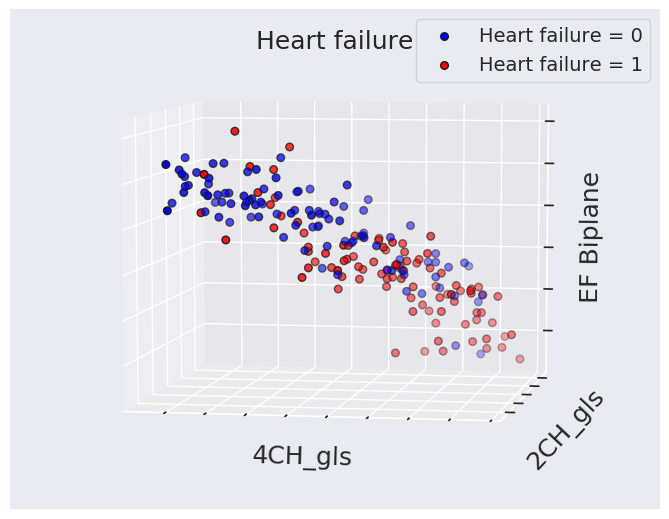
\includegraphics[width=0.99\textwidth]{results/hf/scatter_gls_EF_hf.png}
        \caption{Heart failure.}
        \label{fig:scatter_gls_ef_hf}
    \end{subfigure}
    \begin{subfigure}[b]{0.49\textwidth}
        \centering
        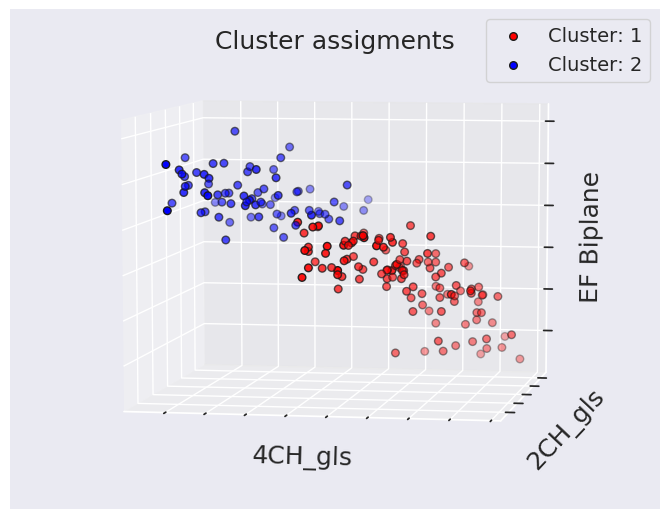
\includegraphics[width=0.99\textwidth]{results/hf/scatter_gls_EF_ward2.png}
        \caption{\textit{Ward/2} cluster assignments.}
        \label{fig:scatter_gls_ef_ward2}
    \end{subfigure}\\
    \begin{subfigure}[b]{0.49\textwidth}
        \centering
        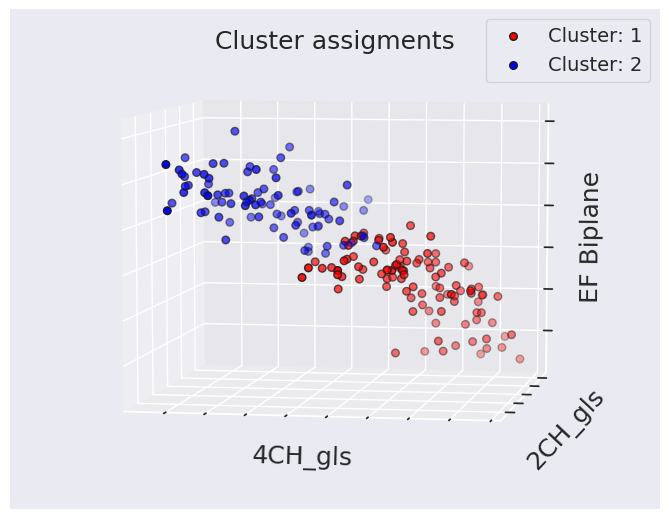
\includegraphics[width=0.99\textwidth]{results/hf/scatter_gls_EF_complete2.png}
        \caption{\textit{Complete/2} cluster assignments.}
        \label{fig:scatter_gls_ef_complete2}
    \end{subfigure}
    \begin{subfigure}[b]{0.49\textwidth}
        \centering
        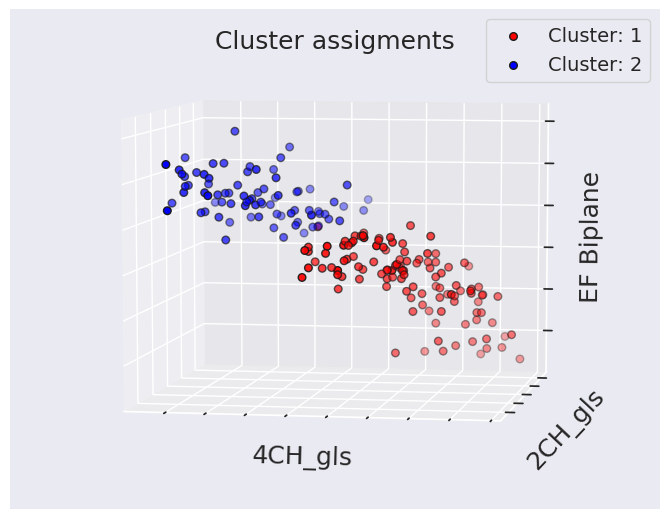
\includegraphics[width=0.99\textwidth]{results/hf/scatter_gls_EF_average2.png}
        \caption{\textit{Average/2} cluster assignments.}
        \label{fig:scatter_gls_ef_average2}
    \end{subfigure}
    \caption{Scatterplot of peak GLS values in each view. Colors in the of the different dots are given by heart failure diagnosis, and cluster assignments of 
             ward/2, complete/2 and average/2 methods. Numbers are not included on the axes because the point of the figure is to illustrate the separability 
             of clusters, and heart failure.}
             \label{fig:scatter_gls_ef_hf_cluster_assignments}
\end{figure}

\clearpage

\subsection{Deep Neural Network}

\begin{figure}[H]
    \centering
    % \includegraphics[width=\textwidth]{results/dl_hf_dor_sens_spec_dist.png}
    %% Creator: Matplotlib, PGF backend
%%
%% To include the figure in your LaTeX document, write
%%   \input{<filename>.pgf}
%%
%% Make sure the required packages are loaded in your preamble
%%   \usepackage{pgf}
%%
%% Figures using additional raster images can only be included by \input if
%% they are in the same directory as the main LaTeX file. For loading figures
%% from other directories you can use the `import` package
%%   \usepackage{import}
%% and then include the figures with
%%   \import{<path to file>}{<filename>.pgf}
%%
%% Matplotlib used the following preamble
%%
\begingroup%
\makeatletter%
\begin{pgfpicture}%
\pgfpathrectangle{\pgfpointorigin}{\pgfqpoint{6.246672in}{2.540000in}}%
\pgfusepath{use as bounding box, clip}%
\begin{pgfscope}%
\pgfsetbuttcap%
\pgfsetmiterjoin%
\definecolor{currentfill}{rgb}{1.000000,1.000000,1.000000}%
\pgfsetfillcolor{currentfill}%
\pgfsetlinewidth{0.000000pt}%
\definecolor{currentstroke}{rgb}{1.000000,1.000000,1.000000}%
\pgfsetstrokecolor{currentstroke}%
\pgfsetdash{}{0pt}%
\pgfpathmoveto{\pgfqpoint{0.000000in}{0.000000in}}%
\pgfpathlineto{\pgfqpoint{6.246672in}{0.000000in}}%
\pgfpathlineto{\pgfqpoint{6.246672in}{2.540000in}}%
\pgfpathlineto{\pgfqpoint{0.000000in}{2.540000in}}%
\pgfpathclose%
\pgfusepath{fill}%
\end{pgfscope}%
\begin{pgfscope}%
\pgfsetbuttcap%
\pgfsetmiterjoin%
\definecolor{currentfill}{rgb}{0.917647,0.917647,0.949020}%
\pgfsetfillcolor{currentfill}%
\pgfsetlinewidth{0.000000pt}%
\definecolor{currentstroke}{rgb}{0.000000,0.000000,0.000000}%
\pgfsetstrokecolor{currentstroke}%
\pgfsetstrokeopacity{0.000000}%
\pgfsetdash{}{0pt}%
\pgfpathmoveto{\pgfqpoint{0.574769in}{0.557870in}}%
\pgfpathlineto{\pgfqpoint{2.999734in}{0.557870in}}%
\pgfpathlineto{\pgfqpoint{2.999734in}{2.242604in}}%
\pgfpathlineto{\pgfqpoint{0.574769in}{2.242604in}}%
\pgfpathclose%
\pgfusepath{fill}%
\end{pgfscope}%
\begin{pgfscope}%
\pgfpathrectangle{\pgfqpoint{0.574769in}{0.557870in}}{\pgfqpoint{2.424965in}{1.684734in}}%
\pgfusepath{clip}%
\pgfsetroundcap%
\pgfsetroundjoin%
\pgfsetlinewidth{1.003750pt}%
\definecolor{currentstroke}{rgb}{1.000000,1.000000,1.000000}%
\pgfsetstrokecolor{currentstroke}%
\pgfsetdash{}{0pt}%
\pgfpathmoveto{\pgfqpoint{0.684994in}{0.557870in}}%
\pgfpathlineto{\pgfqpoint{0.684994in}{2.242604in}}%
\pgfusepath{stroke}%
\end{pgfscope}%
\begin{pgfscope}%
\definecolor{textcolor}{rgb}{0.150000,0.150000,0.150000}%
\pgfsetstrokecolor{textcolor}%
\pgfsetfillcolor{textcolor}%
\pgftext[x=0.684994in,y=0.425926in,,top]{\color{textcolor}\sffamily\fontsize{11.000000}{13.200000}\selectfont \(\displaystyle 0.0\)}%
\end{pgfscope}%
\begin{pgfscope}%
\pgfpathrectangle{\pgfqpoint{0.574769in}{0.557870in}}{\pgfqpoint{2.424965in}{1.684734in}}%
\pgfusepath{clip}%
\pgfsetroundcap%
\pgfsetroundjoin%
\pgfsetlinewidth{1.003750pt}%
\definecolor{currentstroke}{rgb}{1.000000,1.000000,1.000000}%
\pgfsetstrokecolor{currentstroke}%
\pgfsetdash{}{0pt}%
\pgfpathmoveto{\pgfqpoint{1.496956in}{0.557870in}}%
\pgfpathlineto{\pgfqpoint{1.496956in}{2.242604in}}%
\pgfusepath{stroke}%
\end{pgfscope}%
\begin{pgfscope}%
\definecolor{textcolor}{rgb}{0.150000,0.150000,0.150000}%
\pgfsetstrokecolor{textcolor}%
\pgfsetfillcolor{textcolor}%
\pgftext[x=1.496956in,y=0.425926in,,top]{\color{textcolor}\sffamily\fontsize{11.000000}{13.200000}\selectfont \(\displaystyle 0.5\)}%
\end{pgfscope}%
\begin{pgfscope}%
\pgfpathrectangle{\pgfqpoint{0.574769in}{0.557870in}}{\pgfqpoint{2.424965in}{1.684734in}}%
\pgfusepath{clip}%
\pgfsetroundcap%
\pgfsetroundjoin%
\pgfsetlinewidth{1.003750pt}%
\definecolor{currentstroke}{rgb}{1.000000,1.000000,1.000000}%
\pgfsetstrokecolor{currentstroke}%
\pgfsetdash{}{0pt}%
\pgfpathmoveto{\pgfqpoint{2.308918in}{0.557870in}}%
\pgfpathlineto{\pgfqpoint{2.308918in}{2.242604in}}%
\pgfusepath{stroke}%
\end{pgfscope}%
\begin{pgfscope}%
\definecolor{textcolor}{rgb}{0.150000,0.150000,0.150000}%
\pgfsetstrokecolor{textcolor}%
\pgfsetfillcolor{textcolor}%
\pgftext[x=2.308918in,y=0.425926in,,top]{\color{textcolor}\sffamily\fontsize{11.000000}{13.200000}\selectfont \(\displaystyle 1.0\)}%
\end{pgfscope}%
\begin{pgfscope}%
\definecolor{textcolor}{rgb}{0.150000,0.150000,0.150000}%
\pgfsetstrokecolor{textcolor}%
\pgfsetfillcolor{textcolor}%
\pgftext[x=1.787251in,y=0.235185in,,top]{\color{textcolor}\sffamily\fontsize{11.000000}{13.200000}\selectfont DOR}%
\end{pgfscope}%
\begin{pgfscope}%
\pgfpathrectangle{\pgfqpoint{0.574769in}{0.557870in}}{\pgfqpoint{2.424965in}{1.684734in}}%
\pgfusepath{clip}%
\pgfsetroundcap%
\pgfsetroundjoin%
\pgfsetlinewidth{1.003750pt}%
\definecolor{currentstroke}{rgb}{1.000000,1.000000,1.000000}%
\pgfsetstrokecolor{currentstroke}%
\pgfsetdash{}{0pt}%
\pgfpathmoveto{\pgfqpoint{0.574769in}{0.557870in}}%
\pgfpathlineto{\pgfqpoint{2.999734in}{0.557870in}}%
\pgfusepath{stroke}%
\end{pgfscope}%
\begin{pgfscope}%
\definecolor{textcolor}{rgb}{0.150000,0.150000,0.150000}%
\pgfsetstrokecolor{textcolor}%
\pgfsetfillcolor{textcolor}%
\pgftext[x=0.366783in,y=0.505064in,left,base]{\color{textcolor}\sffamily\fontsize{11.000000}{13.200000}\selectfont \(\displaystyle 0\)}%
\end{pgfscope}%
\begin{pgfscope}%
\pgfpathrectangle{\pgfqpoint{0.574769in}{0.557870in}}{\pgfqpoint{2.424965in}{1.684734in}}%
\pgfusepath{clip}%
\pgfsetroundcap%
\pgfsetroundjoin%
\pgfsetlinewidth{1.003750pt}%
\definecolor{currentstroke}{rgb}{1.000000,1.000000,1.000000}%
\pgfsetstrokecolor{currentstroke}%
\pgfsetdash{}{0pt}%
\pgfpathmoveto{\pgfqpoint{0.574769in}{1.174989in}}%
\pgfpathlineto{\pgfqpoint{2.999734in}{1.174989in}}%
\pgfusepath{stroke}%
\end{pgfscope}%
\begin{pgfscope}%
\definecolor{textcolor}{rgb}{0.150000,0.150000,0.150000}%
\pgfsetstrokecolor{textcolor}%
\pgfsetfillcolor{textcolor}%
\pgftext[x=0.366783in,y=1.122182in,left,base]{\color{textcolor}\sffamily\fontsize{11.000000}{13.200000}\selectfont \(\displaystyle 5\)}%
\end{pgfscope}%
\begin{pgfscope}%
\pgfpathrectangle{\pgfqpoint{0.574769in}{0.557870in}}{\pgfqpoint{2.424965in}{1.684734in}}%
\pgfusepath{clip}%
\pgfsetroundcap%
\pgfsetroundjoin%
\pgfsetlinewidth{1.003750pt}%
\definecolor{currentstroke}{rgb}{1.000000,1.000000,1.000000}%
\pgfsetstrokecolor{currentstroke}%
\pgfsetdash{}{0pt}%
\pgfpathmoveto{\pgfqpoint{0.574769in}{1.792108in}}%
\pgfpathlineto{\pgfqpoint{2.999734in}{1.792108in}}%
\pgfusepath{stroke}%
\end{pgfscope}%
\begin{pgfscope}%
\definecolor{textcolor}{rgb}{0.150000,0.150000,0.150000}%
\pgfsetstrokecolor{textcolor}%
\pgfsetfillcolor{textcolor}%
\pgftext[x=0.290741in,y=1.739301in,left,base]{\color{textcolor}\sffamily\fontsize{11.000000}{13.200000}\selectfont \(\displaystyle 10\)}%
\end{pgfscope}%
\begin{pgfscope}%
\definecolor{textcolor}{rgb}{0.150000,0.150000,0.150000}%
\pgfsetstrokecolor{textcolor}%
\pgfsetfillcolor{textcolor}%
\pgftext[x=0.235185in,y=1.400237in,,bottom,rotate=90.000000]{\color{textcolor}\sffamily\fontsize{11.000000}{13.200000}\selectfont Occurance}%
\end{pgfscope}%
\begin{pgfscope}%
\pgfpathrectangle{\pgfqpoint{0.574769in}{0.557870in}}{\pgfqpoint{2.424965in}{1.684734in}}%
\pgfusepath{clip}%
\pgfsetbuttcap%
\pgfsetmiterjoin%
\definecolor{currentfill}{rgb}{0.298039,0.447059,0.690196}%
\pgfsetfillcolor{currentfill}%
\pgfsetfillopacity{0.400000}%
\pgfsetlinewidth{1.003750pt}%
\definecolor{currentstroke}{rgb}{1.000000,1.000000,1.000000}%
\pgfsetstrokecolor{currentstroke}%
\pgfsetstrokeopacity{0.400000}%
\pgfsetdash{}{0pt}%
\pgfpathmoveto{\pgfqpoint{0.684994in}{0.557870in}}%
\pgfpathlineto{\pgfqpoint{0.905446in}{0.557870in}}%
\pgfpathlineto{\pgfqpoint{0.905446in}{2.162379in}}%
\pgfpathlineto{\pgfqpoint{0.684994in}{2.162379in}}%
\pgfpathclose%
\pgfusepath{stroke,fill}%
\end{pgfscope}%
\begin{pgfscope}%
\pgfpathrectangle{\pgfqpoint{0.574769in}{0.557870in}}{\pgfqpoint{2.424965in}{1.684734in}}%
\pgfusepath{clip}%
\pgfsetbuttcap%
\pgfsetmiterjoin%
\definecolor{currentfill}{rgb}{0.298039,0.447059,0.690196}%
\pgfsetfillcolor{currentfill}%
\pgfsetfillopacity{0.400000}%
\pgfsetlinewidth{1.003750pt}%
\definecolor{currentstroke}{rgb}{1.000000,1.000000,1.000000}%
\pgfsetstrokecolor{currentstroke}%
\pgfsetstrokeopacity{0.400000}%
\pgfsetdash{}{0pt}%
\pgfpathmoveto{\pgfqpoint{0.905446in}{0.557870in}}%
\pgfpathlineto{\pgfqpoint{1.125897in}{0.557870in}}%
\pgfpathlineto{\pgfqpoint{1.125897in}{1.174989in}}%
\pgfpathlineto{\pgfqpoint{0.905446in}{1.174989in}}%
\pgfpathclose%
\pgfusepath{stroke,fill}%
\end{pgfscope}%
\begin{pgfscope}%
\pgfpathrectangle{\pgfqpoint{0.574769in}{0.557870in}}{\pgfqpoint{2.424965in}{1.684734in}}%
\pgfusepath{clip}%
\pgfsetbuttcap%
\pgfsetmiterjoin%
\definecolor{currentfill}{rgb}{0.298039,0.447059,0.690196}%
\pgfsetfillcolor{currentfill}%
\pgfsetfillopacity{0.400000}%
\pgfsetlinewidth{1.003750pt}%
\definecolor{currentstroke}{rgb}{1.000000,1.000000,1.000000}%
\pgfsetstrokecolor{currentstroke}%
\pgfsetstrokeopacity{0.400000}%
\pgfsetdash{}{0pt}%
\pgfpathmoveto{\pgfqpoint{1.125897in}{0.557870in}}%
\pgfpathlineto{\pgfqpoint{1.346348in}{0.557870in}}%
\pgfpathlineto{\pgfqpoint{1.346348in}{1.298413in}}%
\pgfpathlineto{\pgfqpoint{1.125897in}{1.298413in}}%
\pgfpathclose%
\pgfusepath{stroke,fill}%
\end{pgfscope}%
\begin{pgfscope}%
\pgfpathrectangle{\pgfqpoint{0.574769in}{0.557870in}}{\pgfqpoint{2.424965in}{1.684734in}}%
\pgfusepath{clip}%
\pgfsetbuttcap%
\pgfsetmiterjoin%
\definecolor{currentfill}{rgb}{0.298039,0.447059,0.690196}%
\pgfsetfillcolor{currentfill}%
\pgfsetfillopacity{0.400000}%
\pgfsetlinewidth{1.003750pt}%
\definecolor{currentstroke}{rgb}{1.000000,1.000000,1.000000}%
\pgfsetstrokecolor{currentstroke}%
\pgfsetstrokeopacity{0.400000}%
\pgfsetdash{}{0pt}%
\pgfpathmoveto{\pgfqpoint{1.346348in}{0.557870in}}%
\pgfpathlineto{\pgfqpoint{1.566800in}{0.557870in}}%
\pgfpathlineto{\pgfqpoint{1.566800in}{0.928141in}}%
\pgfpathlineto{\pgfqpoint{1.346348in}{0.928141in}}%
\pgfpathclose%
\pgfusepath{stroke,fill}%
\end{pgfscope}%
\begin{pgfscope}%
\pgfpathrectangle{\pgfqpoint{0.574769in}{0.557870in}}{\pgfqpoint{2.424965in}{1.684734in}}%
\pgfusepath{clip}%
\pgfsetbuttcap%
\pgfsetmiterjoin%
\definecolor{currentfill}{rgb}{0.298039,0.447059,0.690196}%
\pgfsetfillcolor{currentfill}%
\pgfsetfillopacity{0.400000}%
\pgfsetlinewidth{1.003750pt}%
\definecolor{currentstroke}{rgb}{1.000000,1.000000,1.000000}%
\pgfsetstrokecolor{currentstroke}%
\pgfsetstrokeopacity{0.400000}%
\pgfsetdash{}{0pt}%
\pgfpathmoveto{\pgfqpoint{1.566800in}{0.557870in}}%
\pgfpathlineto{\pgfqpoint{1.787251in}{0.557870in}}%
\pgfpathlineto{\pgfqpoint{1.787251in}{0.557870in}}%
\pgfpathlineto{\pgfqpoint{1.566800in}{0.557870in}}%
\pgfpathclose%
\pgfusepath{stroke,fill}%
\end{pgfscope}%
\begin{pgfscope}%
\pgfpathrectangle{\pgfqpoint{0.574769in}{0.557870in}}{\pgfqpoint{2.424965in}{1.684734in}}%
\pgfusepath{clip}%
\pgfsetbuttcap%
\pgfsetmiterjoin%
\definecolor{currentfill}{rgb}{0.298039,0.447059,0.690196}%
\pgfsetfillcolor{currentfill}%
\pgfsetfillopacity{0.400000}%
\pgfsetlinewidth{1.003750pt}%
\definecolor{currentstroke}{rgb}{1.000000,1.000000,1.000000}%
\pgfsetstrokecolor{currentstroke}%
\pgfsetstrokeopacity{0.400000}%
\pgfsetdash{}{0pt}%
\pgfpathmoveto{\pgfqpoint{1.787251in}{0.557870in}}%
\pgfpathlineto{\pgfqpoint{2.007703in}{0.557870in}}%
\pgfpathlineto{\pgfqpoint{2.007703in}{0.681294in}}%
\pgfpathlineto{\pgfqpoint{1.787251in}{0.681294in}}%
\pgfpathclose%
\pgfusepath{stroke,fill}%
\end{pgfscope}%
\begin{pgfscope}%
\pgfpathrectangle{\pgfqpoint{0.574769in}{0.557870in}}{\pgfqpoint{2.424965in}{1.684734in}}%
\pgfusepath{clip}%
\pgfsetbuttcap%
\pgfsetmiterjoin%
\definecolor{currentfill}{rgb}{0.298039,0.447059,0.690196}%
\pgfsetfillcolor{currentfill}%
\pgfsetfillopacity{0.400000}%
\pgfsetlinewidth{1.003750pt}%
\definecolor{currentstroke}{rgb}{1.000000,1.000000,1.000000}%
\pgfsetstrokecolor{currentstroke}%
\pgfsetstrokeopacity{0.400000}%
\pgfsetdash{}{0pt}%
\pgfpathmoveto{\pgfqpoint{2.007703in}{0.557870in}}%
\pgfpathlineto{\pgfqpoint{2.228154in}{0.557870in}}%
\pgfpathlineto{\pgfqpoint{2.228154in}{0.804718in}}%
\pgfpathlineto{\pgfqpoint{2.007703in}{0.804718in}}%
\pgfpathclose%
\pgfusepath{stroke,fill}%
\end{pgfscope}%
\begin{pgfscope}%
\pgfpathrectangle{\pgfqpoint{0.574769in}{0.557870in}}{\pgfqpoint{2.424965in}{1.684734in}}%
\pgfusepath{clip}%
\pgfsetbuttcap%
\pgfsetmiterjoin%
\definecolor{currentfill}{rgb}{0.298039,0.447059,0.690196}%
\pgfsetfillcolor{currentfill}%
\pgfsetfillopacity{0.400000}%
\pgfsetlinewidth{1.003750pt}%
\definecolor{currentstroke}{rgb}{1.000000,1.000000,1.000000}%
\pgfsetstrokecolor{currentstroke}%
\pgfsetstrokeopacity{0.400000}%
\pgfsetdash{}{0pt}%
\pgfpathmoveto{\pgfqpoint{2.228154in}{0.557870in}}%
\pgfpathlineto{\pgfqpoint{2.448605in}{0.557870in}}%
\pgfpathlineto{\pgfqpoint{2.448605in}{0.804718in}}%
\pgfpathlineto{\pgfqpoint{2.228154in}{0.804718in}}%
\pgfpathclose%
\pgfusepath{stroke,fill}%
\end{pgfscope}%
\begin{pgfscope}%
\pgfpathrectangle{\pgfqpoint{0.574769in}{0.557870in}}{\pgfqpoint{2.424965in}{1.684734in}}%
\pgfusepath{clip}%
\pgfsetbuttcap%
\pgfsetmiterjoin%
\definecolor{currentfill}{rgb}{0.298039,0.447059,0.690196}%
\pgfsetfillcolor{currentfill}%
\pgfsetfillopacity{0.400000}%
\pgfsetlinewidth{1.003750pt}%
\definecolor{currentstroke}{rgb}{1.000000,1.000000,1.000000}%
\pgfsetstrokecolor{currentstroke}%
\pgfsetstrokeopacity{0.400000}%
\pgfsetdash{}{0pt}%
\pgfpathmoveto{\pgfqpoint{2.448605in}{0.557870in}}%
\pgfpathlineto{\pgfqpoint{2.669057in}{0.557870in}}%
\pgfpathlineto{\pgfqpoint{2.669057in}{0.804718in}}%
\pgfpathlineto{\pgfqpoint{2.448605in}{0.804718in}}%
\pgfpathclose%
\pgfusepath{stroke,fill}%
\end{pgfscope}%
\begin{pgfscope}%
\pgfpathrectangle{\pgfqpoint{0.574769in}{0.557870in}}{\pgfqpoint{2.424965in}{1.684734in}}%
\pgfusepath{clip}%
\pgfsetbuttcap%
\pgfsetmiterjoin%
\definecolor{currentfill}{rgb}{0.298039,0.447059,0.690196}%
\pgfsetfillcolor{currentfill}%
\pgfsetfillopacity{0.400000}%
\pgfsetlinewidth{1.003750pt}%
\definecolor{currentstroke}{rgb}{1.000000,1.000000,1.000000}%
\pgfsetstrokecolor{currentstroke}%
\pgfsetstrokeopacity{0.400000}%
\pgfsetdash{}{0pt}%
\pgfpathmoveto{\pgfqpoint{2.669057in}{0.557870in}}%
\pgfpathlineto{\pgfqpoint{2.889508in}{0.557870in}}%
\pgfpathlineto{\pgfqpoint{2.889508in}{0.804718in}}%
\pgfpathlineto{\pgfqpoint{2.669057in}{0.804718in}}%
\pgfpathclose%
\pgfusepath{stroke,fill}%
\end{pgfscope}%
\begin{pgfscope}%
\pgfsetrectcap%
\pgfsetmiterjoin%
\pgfsetlinewidth{1.254687pt}%
\definecolor{currentstroke}{rgb}{1.000000,1.000000,1.000000}%
\pgfsetstrokecolor{currentstroke}%
\pgfsetdash{}{0pt}%
\pgfpathmoveto{\pgfqpoint{0.574769in}{0.557870in}}%
\pgfpathlineto{\pgfqpoint{0.574769in}{2.242604in}}%
\pgfusepath{stroke}%
\end{pgfscope}%
\begin{pgfscope}%
\pgfsetrectcap%
\pgfsetmiterjoin%
\pgfsetlinewidth{1.254687pt}%
\definecolor{currentstroke}{rgb}{1.000000,1.000000,1.000000}%
\pgfsetstrokecolor{currentstroke}%
\pgfsetdash{}{0pt}%
\pgfpathmoveto{\pgfqpoint{2.999734in}{0.557870in}}%
\pgfpathlineto{\pgfqpoint{2.999734in}{2.242604in}}%
\pgfusepath{stroke}%
\end{pgfscope}%
\begin{pgfscope}%
\pgfsetrectcap%
\pgfsetmiterjoin%
\pgfsetlinewidth{1.254687pt}%
\definecolor{currentstroke}{rgb}{1.000000,1.000000,1.000000}%
\pgfsetstrokecolor{currentstroke}%
\pgfsetdash{}{0pt}%
\pgfpathmoveto{\pgfqpoint{0.574769in}{0.557870in}}%
\pgfpathlineto{\pgfqpoint{2.999734in}{0.557870in}}%
\pgfusepath{stroke}%
\end{pgfscope}%
\begin{pgfscope}%
\pgfsetrectcap%
\pgfsetmiterjoin%
\pgfsetlinewidth{1.254687pt}%
\definecolor{currentstroke}{rgb}{1.000000,1.000000,1.000000}%
\pgfsetstrokecolor{currentstroke}%
\pgfsetdash{}{0pt}%
\pgfpathmoveto{\pgfqpoint{0.574769in}{2.242604in}}%
\pgfpathlineto{\pgfqpoint{2.999734in}{2.242604in}}%
\pgfusepath{stroke}%
\end{pgfscope}%
\begin{pgfscope}%
\definecolor{textcolor}{rgb}{0.150000,0.150000,0.150000}%
\pgfsetstrokecolor{textcolor}%
\pgfsetfillcolor{textcolor}%
\pgftext[x=1.787251in,y=2.325938in,,base]{\color{textcolor}\sffamily\fontsize{11.000000}{13.200000}\selectfont (a)}%
\end{pgfscope}%
\begin{pgfscope}%
\pgfsetbuttcap%
\pgfsetmiterjoin%
\definecolor{currentfill}{rgb}{0.917647,0.917647,0.949020}%
\pgfsetfillcolor{currentfill}%
\pgfsetlinewidth{0.000000pt}%
\definecolor{currentstroke}{rgb}{0.000000,0.000000,0.000000}%
\pgfsetstrokecolor{currentstroke}%
\pgfsetstrokeopacity{0.000000}%
\pgfsetdash{}{0pt}%
\pgfpathmoveto{\pgfqpoint{3.696748in}{0.557870in}}%
\pgfpathlineto{\pgfqpoint{6.121713in}{0.557870in}}%
\pgfpathlineto{\pgfqpoint{6.121713in}{2.242604in}}%
\pgfpathlineto{\pgfqpoint{3.696748in}{2.242604in}}%
\pgfpathclose%
\pgfusepath{fill}%
\end{pgfscope}%
\begin{pgfscope}%
\pgfpathrectangle{\pgfqpoint{3.696748in}{0.557870in}}{\pgfqpoint{2.424965in}{1.684734in}}%
\pgfusepath{clip}%
\pgfsetroundcap%
\pgfsetroundjoin%
\pgfsetlinewidth{1.003750pt}%
\definecolor{currentstroke}{rgb}{1.000000,1.000000,1.000000}%
\pgfsetstrokecolor{currentstroke}%
\pgfsetdash{}{0pt}%
\pgfpathmoveto{\pgfqpoint{3.806973in}{0.557870in}}%
\pgfpathlineto{\pgfqpoint{3.806973in}{2.242604in}}%
\pgfusepath{stroke}%
\end{pgfscope}%
\begin{pgfscope}%
\definecolor{textcolor}{rgb}{0.150000,0.150000,0.150000}%
\pgfsetstrokecolor{textcolor}%
\pgfsetfillcolor{textcolor}%
\pgftext[x=3.806973in,y=0.425926in,,top]{\color{textcolor}\sffamily\fontsize{11.000000}{13.200000}\selectfont \(\displaystyle 0.00\)}%
\end{pgfscope}%
\begin{pgfscope}%
\pgfpathrectangle{\pgfqpoint{3.696748in}{0.557870in}}{\pgfqpoint{2.424965in}{1.684734in}}%
\pgfusepath{clip}%
\pgfsetroundcap%
\pgfsetroundjoin%
\pgfsetlinewidth{1.003750pt}%
\definecolor{currentstroke}{rgb}{1.000000,1.000000,1.000000}%
\pgfsetstrokecolor{currentstroke}%
\pgfsetdash{}{0pt}%
\pgfpathmoveto{\pgfqpoint{4.358102in}{0.557870in}}%
\pgfpathlineto{\pgfqpoint{4.358102in}{2.242604in}}%
\pgfusepath{stroke}%
\end{pgfscope}%
\begin{pgfscope}%
\definecolor{textcolor}{rgb}{0.150000,0.150000,0.150000}%
\pgfsetstrokecolor{textcolor}%
\pgfsetfillcolor{textcolor}%
\pgftext[x=4.358102in,y=0.425926in,,top]{\color{textcolor}\sffamily\fontsize{11.000000}{13.200000}\selectfont \(\displaystyle 0.25\)}%
\end{pgfscope}%
\begin{pgfscope}%
\pgfpathrectangle{\pgfqpoint{3.696748in}{0.557870in}}{\pgfqpoint{2.424965in}{1.684734in}}%
\pgfusepath{clip}%
\pgfsetroundcap%
\pgfsetroundjoin%
\pgfsetlinewidth{1.003750pt}%
\definecolor{currentstroke}{rgb}{1.000000,1.000000,1.000000}%
\pgfsetstrokecolor{currentstroke}%
\pgfsetdash{}{0pt}%
\pgfpathmoveto{\pgfqpoint{4.909230in}{0.557870in}}%
\pgfpathlineto{\pgfqpoint{4.909230in}{2.242604in}}%
\pgfusepath{stroke}%
\end{pgfscope}%
\begin{pgfscope}%
\definecolor{textcolor}{rgb}{0.150000,0.150000,0.150000}%
\pgfsetstrokecolor{textcolor}%
\pgfsetfillcolor{textcolor}%
\pgftext[x=4.909230in,y=0.425926in,,top]{\color{textcolor}\sffamily\fontsize{11.000000}{13.200000}\selectfont \(\displaystyle 0.50\)}%
\end{pgfscope}%
\begin{pgfscope}%
\pgfpathrectangle{\pgfqpoint{3.696748in}{0.557870in}}{\pgfqpoint{2.424965in}{1.684734in}}%
\pgfusepath{clip}%
\pgfsetroundcap%
\pgfsetroundjoin%
\pgfsetlinewidth{1.003750pt}%
\definecolor{currentstroke}{rgb}{1.000000,1.000000,1.000000}%
\pgfsetstrokecolor{currentstroke}%
\pgfsetdash{}{0pt}%
\pgfpathmoveto{\pgfqpoint{5.460359in}{0.557870in}}%
\pgfpathlineto{\pgfqpoint{5.460359in}{2.242604in}}%
\pgfusepath{stroke}%
\end{pgfscope}%
\begin{pgfscope}%
\definecolor{textcolor}{rgb}{0.150000,0.150000,0.150000}%
\pgfsetstrokecolor{textcolor}%
\pgfsetfillcolor{textcolor}%
\pgftext[x=5.460359in,y=0.425926in,,top]{\color{textcolor}\sffamily\fontsize{11.000000}{13.200000}\selectfont \(\displaystyle 0.75\)}%
\end{pgfscope}%
\begin{pgfscope}%
\pgfpathrectangle{\pgfqpoint{3.696748in}{0.557870in}}{\pgfqpoint{2.424965in}{1.684734in}}%
\pgfusepath{clip}%
\pgfsetroundcap%
\pgfsetroundjoin%
\pgfsetlinewidth{1.003750pt}%
\definecolor{currentstroke}{rgb}{1.000000,1.000000,1.000000}%
\pgfsetstrokecolor{currentstroke}%
\pgfsetdash{}{0pt}%
\pgfpathmoveto{\pgfqpoint{6.011487in}{0.557870in}}%
\pgfpathlineto{\pgfqpoint{6.011487in}{2.242604in}}%
\pgfusepath{stroke}%
\end{pgfscope}%
\begin{pgfscope}%
\definecolor{textcolor}{rgb}{0.150000,0.150000,0.150000}%
\pgfsetstrokecolor{textcolor}%
\pgfsetfillcolor{textcolor}%
\pgftext[x=6.011487in,y=0.425926in,,top]{\color{textcolor}\sffamily\fontsize{11.000000}{13.200000}\selectfont \(\displaystyle 1.00\)}%
\end{pgfscope}%
\begin{pgfscope}%
\definecolor{textcolor}{rgb}{0.150000,0.150000,0.150000}%
\pgfsetstrokecolor{textcolor}%
\pgfsetfillcolor{textcolor}%
\pgftext[x=4.909230in,y=0.235185in,,top]{\color{textcolor}\sffamily\fontsize{11.000000}{13.200000}\selectfont Specificity}%
\end{pgfscope}%
\begin{pgfscope}%
\pgfpathrectangle{\pgfqpoint{3.696748in}{0.557870in}}{\pgfqpoint{2.424965in}{1.684734in}}%
\pgfusepath{clip}%
\pgfsetroundcap%
\pgfsetroundjoin%
\pgfsetlinewidth{1.003750pt}%
\definecolor{currentstroke}{rgb}{1.000000,1.000000,1.000000}%
\pgfsetstrokecolor{currentstroke}%
\pgfsetdash{}{0pt}%
\pgfpathmoveto{\pgfqpoint{3.696748in}{0.634449in}}%
\pgfpathlineto{\pgfqpoint{6.121713in}{0.634449in}}%
\pgfusepath{stroke}%
\end{pgfscope}%
\begin{pgfscope}%
\definecolor{textcolor}{rgb}{0.150000,0.150000,0.150000}%
\pgfsetstrokecolor{textcolor}%
\pgfsetfillcolor{textcolor}%
\pgftext[x=3.294433in,y=0.581642in,left,base]{\color{textcolor}\sffamily\fontsize{11.000000}{13.200000}\selectfont \(\displaystyle 0.00\)}%
\end{pgfscope}%
\begin{pgfscope}%
\pgfpathrectangle{\pgfqpoint{3.696748in}{0.557870in}}{\pgfqpoint{2.424965in}{1.684734in}}%
\pgfusepath{clip}%
\pgfsetroundcap%
\pgfsetroundjoin%
\pgfsetlinewidth{1.003750pt}%
\definecolor{currentstroke}{rgb}{1.000000,1.000000,1.000000}%
\pgfsetstrokecolor{currentstroke}%
\pgfsetdash{}{0pt}%
\pgfpathmoveto{\pgfqpoint{3.696748in}{1.017343in}}%
\pgfpathlineto{\pgfqpoint{6.121713in}{1.017343in}}%
\pgfusepath{stroke}%
\end{pgfscope}%
\begin{pgfscope}%
\definecolor{textcolor}{rgb}{0.150000,0.150000,0.150000}%
\pgfsetstrokecolor{textcolor}%
\pgfsetfillcolor{textcolor}%
\pgftext[x=3.294433in,y=0.964536in,left,base]{\color{textcolor}\sffamily\fontsize{11.000000}{13.200000}\selectfont \(\displaystyle 0.25\)}%
\end{pgfscope}%
\begin{pgfscope}%
\pgfpathrectangle{\pgfqpoint{3.696748in}{0.557870in}}{\pgfqpoint{2.424965in}{1.684734in}}%
\pgfusepath{clip}%
\pgfsetroundcap%
\pgfsetroundjoin%
\pgfsetlinewidth{1.003750pt}%
\definecolor{currentstroke}{rgb}{1.000000,1.000000,1.000000}%
\pgfsetstrokecolor{currentstroke}%
\pgfsetdash{}{0pt}%
\pgfpathmoveto{\pgfqpoint{3.696748in}{1.400237in}}%
\pgfpathlineto{\pgfqpoint{6.121713in}{1.400237in}}%
\pgfusepath{stroke}%
\end{pgfscope}%
\begin{pgfscope}%
\definecolor{textcolor}{rgb}{0.150000,0.150000,0.150000}%
\pgfsetstrokecolor{textcolor}%
\pgfsetfillcolor{textcolor}%
\pgftext[x=3.294433in,y=1.347431in,left,base]{\color{textcolor}\sffamily\fontsize{11.000000}{13.200000}\selectfont \(\displaystyle 0.50\)}%
\end{pgfscope}%
\begin{pgfscope}%
\pgfpathrectangle{\pgfqpoint{3.696748in}{0.557870in}}{\pgfqpoint{2.424965in}{1.684734in}}%
\pgfusepath{clip}%
\pgfsetroundcap%
\pgfsetroundjoin%
\pgfsetlinewidth{1.003750pt}%
\definecolor{currentstroke}{rgb}{1.000000,1.000000,1.000000}%
\pgfsetstrokecolor{currentstroke}%
\pgfsetdash{}{0pt}%
\pgfpathmoveto{\pgfqpoint{3.696748in}{1.783131in}}%
\pgfpathlineto{\pgfqpoint{6.121713in}{1.783131in}}%
\pgfusepath{stroke}%
\end{pgfscope}%
\begin{pgfscope}%
\definecolor{textcolor}{rgb}{0.150000,0.150000,0.150000}%
\pgfsetstrokecolor{textcolor}%
\pgfsetfillcolor{textcolor}%
\pgftext[x=3.294433in,y=1.730325in,left,base]{\color{textcolor}\sffamily\fontsize{11.000000}{13.200000}\selectfont \(\displaystyle 0.75\)}%
\end{pgfscope}%
\begin{pgfscope}%
\pgfpathrectangle{\pgfqpoint{3.696748in}{0.557870in}}{\pgfqpoint{2.424965in}{1.684734in}}%
\pgfusepath{clip}%
\pgfsetroundcap%
\pgfsetroundjoin%
\pgfsetlinewidth{1.003750pt}%
\definecolor{currentstroke}{rgb}{1.000000,1.000000,1.000000}%
\pgfsetstrokecolor{currentstroke}%
\pgfsetdash{}{0pt}%
\pgfpathmoveto{\pgfqpoint{3.696748in}{2.166025in}}%
\pgfpathlineto{\pgfqpoint{6.121713in}{2.166025in}}%
\pgfusepath{stroke}%
\end{pgfscope}%
\begin{pgfscope}%
\definecolor{textcolor}{rgb}{0.150000,0.150000,0.150000}%
\pgfsetstrokecolor{textcolor}%
\pgfsetfillcolor{textcolor}%
\pgftext[x=3.294433in,y=2.113219in,left,base]{\color{textcolor}\sffamily\fontsize{11.000000}{13.200000}\selectfont \(\displaystyle 1.00\)}%
\end{pgfscope}%
\begin{pgfscope}%
\definecolor{textcolor}{rgb}{0.150000,0.150000,0.150000}%
\pgfsetstrokecolor{textcolor}%
\pgfsetfillcolor{textcolor}%
\pgftext[x=3.238877in,y=1.400237in,,bottom,rotate=90.000000]{\color{textcolor}\sffamily\fontsize{11.000000}{13.200000}\selectfont Sensitivity}%
\end{pgfscope}%
\begin{pgfscope}%
\pgfpathrectangle{\pgfqpoint{3.696748in}{0.557870in}}{\pgfqpoint{2.424965in}{1.684734in}}%
\pgfusepath{clip}%
\pgfsetbuttcap%
\pgfsetroundjoin%
\definecolor{currentfill}{rgb}{0.298039,0.447059,0.690196}%
\pgfsetfillcolor{currentfill}%
\pgfsetlinewidth{1.003750pt}%
\definecolor{currentstroke}{rgb}{0.298039,0.447059,0.690196}%
\pgfsetstrokecolor{currentstroke}%
\pgfsetdash{}{0pt}%
\pgfpathmoveto{\pgfqpoint{5.151727in}{1.315034in}}%
\pgfpathcurveto{\pgfqpoint{5.159963in}{1.315034in}}{\pgfqpoint{5.167863in}{1.318306in}}{\pgfqpoint{5.173687in}{1.324130in}}%
\pgfpathcurveto{\pgfqpoint{5.179511in}{1.329954in}}{\pgfqpoint{5.182783in}{1.337854in}}{\pgfqpoint{5.182783in}{1.346091in}}%
\pgfpathcurveto{\pgfqpoint{5.182783in}{1.354327in}}{\pgfqpoint{5.179511in}{1.362227in}}{\pgfqpoint{5.173687in}{1.368051in}}%
\pgfpathcurveto{\pgfqpoint{5.167863in}{1.373875in}}{\pgfqpoint{5.159963in}{1.377147in}}{\pgfqpoint{5.151727in}{1.377147in}}%
\pgfpathcurveto{\pgfqpoint{5.143490in}{1.377147in}}{\pgfqpoint{5.135590in}{1.373875in}}{\pgfqpoint{5.129766in}{1.368051in}}%
\pgfpathcurveto{\pgfqpoint{5.123943in}{1.362227in}}{\pgfqpoint{5.120670in}{1.354327in}}{\pgfqpoint{5.120670in}{1.346091in}}%
\pgfpathcurveto{\pgfqpoint{5.120670in}{1.337854in}}{\pgfqpoint{5.123943in}{1.329954in}}{\pgfqpoint{5.129766in}{1.324130in}}%
\pgfpathcurveto{\pgfqpoint{5.135590in}{1.318306in}}{\pgfqpoint{5.143490in}{1.315034in}}{\pgfqpoint{5.151727in}{1.315034in}}%
\pgfpathclose%
\pgfusepath{stroke,fill}%
\end{pgfscope}%
\begin{pgfscope}%
\pgfpathrectangle{\pgfqpoint{3.696748in}{0.557870in}}{\pgfqpoint{2.424965in}{1.684734in}}%
\pgfusepath{clip}%
\pgfsetbuttcap%
\pgfsetroundjoin%
\definecolor{currentfill}{rgb}{0.298039,0.447059,0.690196}%
\pgfsetfillcolor{currentfill}%
\pgfsetlinewidth{1.003750pt}%
\definecolor{currentstroke}{rgb}{0.298039,0.447059,0.690196}%
\pgfsetstrokecolor{currentstroke}%
\pgfsetdash{}{0pt}%
\pgfpathmoveto{\pgfqpoint{5.085591in}{1.345975in}}%
\pgfpathcurveto{\pgfqpoint{5.093828in}{1.345975in}}{\pgfqpoint{5.101728in}{1.349247in}}{\pgfqpoint{5.107552in}{1.355071in}}%
\pgfpathcurveto{\pgfqpoint{5.113376in}{1.360895in}}{\pgfqpoint{5.116648in}{1.368795in}}{\pgfqpoint{5.116648in}{1.377032in}}%
\pgfpathcurveto{\pgfqpoint{5.116648in}{1.385268in}}{\pgfqpoint{5.113376in}{1.393168in}}{\pgfqpoint{5.107552in}{1.398992in}}%
\pgfpathcurveto{\pgfqpoint{5.101728in}{1.404816in}}{\pgfqpoint{5.093828in}{1.408088in}}{\pgfqpoint{5.085591in}{1.408088in}}%
\pgfpathcurveto{\pgfqpoint{5.077355in}{1.408088in}}{\pgfqpoint{5.069455in}{1.404816in}}{\pgfqpoint{5.063631in}{1.398992in}}%
\pgfpathcurveto{\pgfqpoint{5.057807in}{1.393168in}}{\pgfqpoint{5.054535in}{1.385268in}}{\pgfqpoint{5.054535in}{1.377032in}}%
\pgfpathcurveto{\pgfqpoint{5.054535in}{1.368795in}}{\pgfqpoint{5.057807in}{1.360895in}}{\pgfqpoint{5.063631in}{1.355071in}}%
\pgfpathcurveto{\pgfqpoint{5.069455in}{1.349247in}}{\pgfqpoint{5.077355in}{1.345975in}}{\pgfqpoint{5.085591in}{1.345975in}}%
\pgfpathclose%
\pgfusepath{stroke,fill}%
\end{pgfscope}%
\begin{pgfscope}%
\pgfpathrectangle{\pgfqpoint{3.696748in}{0.557870in}}{\pgfqpoint{2.424965in}{1.684734in}}%
\pgfusepath{clip}%
\pgfsetbuttcap%
\pgfsetroundjoin%
\definecolor{currentfill}{rgb}{0.298039,0.447059,0.690196}%
\pgfsetfillcolor{currentfill}%
\pgfsetlinewidth{1.003750pt}%
\definecolor{currentstroke}{rgb}{0.298039,0.447059,0.690196}%
\pgfsetstrokecolor{currentstroke}%
\pgfsetdash{}{0pt}%
\pgfpathmoveto{\pgfqpoint{5.306043in}{1.154760in}}%
\pgfpathcurveto{\pgfqpoint{5.314279in}{1.154760in}}{\pgfqpoint{5.322179in}{1.158032in}}{\pgfqpoint{5.328003in}{1.163856in}}%
\pgfpathcurveto{\pgfqpoint{5.333827in}{1.169680in}}{\pgfqpoint{5.337099in}{1.177580in}}{\pgfqpoint{5.337099in}{1.185817in}}%
\pgfpathcurveto{\pgfqpoint{5.337099in}{1.194053in}}{\pgfqpoint{5.333827in}{1.201953in}}{\pgfqpoint{5.328003in}{1.207777in}}%
\pgfpathcurveto{\pgfqpoint{5.322179in}{1.213601in}}{\pgfqpoint{5.314279in}{1.216873in}}{\pgfqpoint{5.306043in}{1.216873in}}%
\pgfpathcurveto{\pgfqpoint{5.297806in}{1.216873in}}{\pgfqpoint{5.289906in}{1.213601in}}{\pgfqpoint{5.284082in}{1.207777in}}%
\pgfpathcurveto{\pgfqpoint{5.278259in}{1.201953in}}{\pgfqpoint{5.274986in}{1.194053in}}{\pgfqpoint{5.274986in}{1.185817in}}%
\pgfpathcurveto{\pgfqpoint{5.274986in}{1.177580in}}{\pgfqpoint{5.278259in}{1.169680in}}{\pgfqpoint{5.284082in}{1.163856in}}%
\pgfpathcurveto{\pgfqpoint{5.289906in}{1.158032in}}{\pgfqpoint{5.297806in}{1.154760in}}{\pgfqpoint{5.306043in}{1.154760in}}%
\pgfpathclose%
\pgfusepath{stroke,fill}%
\end{pgfscope}%
\begin{pgfscope}%
\pgfpathrectangle{\pgfqpoint{3.696748in}{0.557870in}}{\pgfqpoint{2.424965in}{1.684734in}}%
\pgfusepath{clip}%
\pgfsetbuttcap%
\pgfsetroundjoin%
\definecolor{currentfill}{rgb}{0.298039,0.447059,0.690196}%
\pgfsetfillcolor{currentfill}%
\pgfsetlinewidth{1.003750pt}%
\definecolor{currentstroke}{rgb}{0.298039,0.447059,0.690196}%
\pgfsetstrokecolor{currentstroke}%
\pgfsetdash{}{0pt}%
\pgfpathmoveto{\pgfqpoint{4.688779in}{1.572349in}}%
\pgfpathcurveto{\pgfqpoint{4.697015in}{1.572349in}}{\pgfqpoint{4.704915in}{1.575621in}}{\pgfqpoint{4.710739in}{1.581445in}}%
\pgfpathcurveto{\pgfqpoint{4.716563in}{1.587269in}}{\pgfqpoint{4.719835in}{1.595169in}}{\pgfqpoint{4.719835in}{1.603406in}}%
\pgfpathcurveto{\pgfqpoint{4.719835in}{1.611642in}}{\pgfqpoint{4.716563in}{1.619542in}}{\pgfqpoint{4.710739in}{1.625366in}}%
\pgfpathcurveto{\pgfqpoint{4.704915in}{1.631190in}}{\pgfqpoint{4.697015in}{1.634462in}}{\pgfqpoint{4.688779in}{1.634462in}}%
\pgfpathcurveto{\pgfqpoint{4.680543in}{1.634462in}}{\pgfqpoint{4.672643in}{1.631190in}}{\pgfqpoint{4.666819in}{1.625366in}}%
\pgfpathcurveto{\pgfqpoint{4.660995in}{1.619542in}}{\pgfqpoint{4.657722in}{1.611642in}}{\pgfqpoint{4.657722in}{1.603406in}}%
\pgfpathcurveto{\pgfqpoint{4.657722in}{1.595169in}}{\pgfqpoint{4.660995in}{1.587269in}}{\pgfqpoint{4.666819in}{1.581445in}}%
\pgfpathcurveto{\pgfqpoint{4.672643in}{1.575621in}}{\pgfqpoint{4.680543in}{1.572349in}}{\pgfqpoint{4.688779in}{1.572349in}}%
\pgfpathclose%
\pgfusepath{stroke,fill}%
\end{pgfscope}%
\begin{pgfscope}%
\pgfpathrectangle{\pgfqpoint{3.696748in}{0.557870in}}{\pgfqpoint{2.424965in}{1.684734in}}%
\pgfusepath{clip}%
\pgfsetbuttcap%
\pgfsetroundjoin%
\definecolor{currentfill}{rgb}{0.298039,0.447059,0.690196}%
\pgfsetfillcolor{currentfill}%
\pgfsetlinewidth{1.003750pt}%
\definecolor{currentstroke}{rgb}{0.298039,0.447059,0.690196}%
\pgfsetstrokecolor{currentstroke}%
\pgfsetdash{}{0pt}%
\pgfpathmoveto{\pgfqpoint{4.693324in}{1.531621in}}%
\pgfpathcurveto{\pgfqpoint{4.701561in}{1.531621in}}{\pgfqpoint{4.709461in}{1.534893in}}{\pgfqpoint{4.715285in}{1.540717in}}%
\pgfpathcurveto{\pgfqpoint{4.721108in}{1.546541in}}{\pgfqpoint{4.724381in}{1.554441in}}{\pgfqpoint{4.724381in}{1.562677in}}%
\pgfpathcurveto{\pgfqpoint{4.724381in}{1.570913in}}{\pgfqpoint{4.721108in}{1.578813in}}{\pgfqpoint{4.715285in}{1.584637in}}%
\pgfpathcurveto{\pgfqpoint{4.709461in}{1.590461in}}{\pgfqpoint{4.701561in}{1.593734in}}{\pgfqpoint{4.693324in}{1.593734in}}%
\pgfpathcurveto{\pgfqpoint{4.685088in}{1.593734in}}{\pgfqpoint{4.677188in}{1.590461in}}{\pgfqpoint{4.671364in}{1.584637in}}%
\pgfpathcurveto{\pgfqpoint{4.665540in}{1.578813in}}{\pgfqpoint{4.662268in}{1.570913in}}{\pgfqpoint{4.662268in}{1.562677in}}%
\pgfpathcurveto{\pgfqpoint{4.662268in}{1.554441in}}{\pgfqpoint{4.665540in}{1.546541in}}{\pgfqpoint{4.671364in}{1.540717in}}%
\pgfpathcurveto{\pgfqpoint{4.677188in}{1.534893in}}{\pgfqpoint{4.685088in}{1.531621in}}{\pgfqpoint{4.693324in}{1.531621in}}%
\pgfpathclose%
\pgfusepath{stroke,fill}%
\end{pgfscope}%
\begin{pgfscope}%
\pgfpathrectangle{\pgfqpoint{3.696748in}{0.557870in}}{\pgfqpoint{2.424965in}{1.684734in}}%
\pgfusepath{clip}%
\pgfsetbuttcap%
\pgfsetroundjoin%
\definecolor{currentfill}{rgb}{0.298039,0.447059,0.690196}%
\pgfsetfillcolor{currentfill}%
\pgfsetlinewidth{1.003750pt}%
\definecolor{currentstroke}{rgb}{0.298039,0.447059,0.690196}%
\pgfsetstrokecolor{currentstroke}%
\pgfsetdash{}{0pt}%
\pgfpathmoveto{\pgfqpoint{4.953321in}{1.345975in}}%
\pgfpathcurveto{\pgfqpoint{4.961557in}{1.345975in}}{\pgfqpoint{4.969457in}{1.349247in}}{\pgfqpoint{4.975281in}{1.355071in}}%
\pgfpathcurveto{\pgfqpoint{4.981105in}{1.360895in}}{\pgfqpoint{4.984377in}{1.368795in}}{\pgfqpoint{4.984377in}{1.377032in}}%
\pgfpathcurveto{\pgfqpoint{4.984377in}{1.385268in}}{\pgfqpoint{4.981105in}{1.393168in}}{\pgfqpoint{4.975281in}{1.398992in}}%
\pgfpathcurveto{\pgfqpoint{4.969457in}{1.404816in}}{\pgfqpoint{4.961557in}{1.408088in}}{\pgfqpoint{4.953321in}{1.408088in}}%
\pgfpathcurveto{\pgfqpoint{4.945084in}{1.408088in}}{\pgfqpoint{4.937184in}{1.404816in}}{\pgfqpoint{4.931360in}{1.398992in}}%
\pgfpathcurveto{\pgfqpoint{4.925536in}{1.393168in}}{\pgfqpoint{4.922264in}{1.385268in}}{\pgfqpoint{4.922264in}{1.377032in}}%
\pgfpathcurveto{\pgfqpoint{4.922264in}{1.368795in}}{\pgfqpoint{4.925536in}{1.360895in}}{\pgfqpoint{4.931360in}{1.355071in}}%
\pgfpathcurveto{\pgfqpoint{4.937184in}{1.349247in}}{\pgfqpoint{4.945084in}{1.345975in}}{\pgfqpoint{4.953321in}{1.345975in}}%
\pgfpathclose%
\pgfusepath{stroke,fill}%
\end{pgfscope}%
\begin{pgfscope}%
\pgfpathrectangle{\pgfqpoint{3.696748in}{0.557870in}}{\pgfqpoint{2.424965in}{1.684734in}}%
\pgfusepath{clip}%
\pgfsetbuttcap%
\pgfsetroundjoin%
\definecolor{currentfill}{rgb}{0.298039,0.447059,0.690196}%
\pgfsetfillcolor{currentfill}%
\pgfsetlinewidth{1.003750pt}%
\definecolor{currentstroke}{rgb}{0.298039,0.447059,0.690196}%
\pgfsetstrokecolor{currentstroke}%
\pgfsetdash{}{0pt}%
\pgfpathmoveto{\pgfqpoint{4.909230in}{1.345975in}}%
\pgfpathcurveto{\pgfqpoint{4.917467in}{1.345975in}}{\pgfqpoint{4.925367in}{1.349247in}}{\pgfqpoint{4.931191in}{1.355071in}}%
\pgfpathcurveto{\pgfqpoint{4.937014in}{1.360895in}}{\pgfqpoint{4.940287in}{1.368795in}}{\pgfqpoint{4.940287in}{1.377032in}}%
\pgfpathcurveto{\pgfqpoint{4.940287in}{1.385268in}}{\pgfqpoint{4.937014in}{1.393168in}}{\pgfqpoint{4.931191in}{1.398992in}}%
\pgfpathcurveto{\pgfqpoint{4.925367in}{1.404816in}}{\pgfqpoint{4.917467in}{1.408088in}}{\pgfqpoint{4.909230in}{1.408088in}}%
\pgfpathcurveto{\pgfqpoint{4.900994in}{1.408088in}}{\pgfqpoint{4.893094in}{1.404816in}}{\pgfqpoint{4.887270in}{1.398992in}}%
\pgfpathcurveto{\pgfqpoint{4.881446in}{1.393168in}}{\pgfqpoint{4.878174in}{1.385268in}}{\pgfqpoint{4.878174in}{1.377032in}}%
\pgfpathcurveto{\pgfqpoint{4.878174in}{1.368795in}}{\pgfqpoint{4.881446in}{1.360895in}}{\pgfqpoint{4.887270in}{1.355071in}}%
\pgfpathcurveto{\pgfqpoint{4.893094in}{1.349247in}}{\pgfqpoint{4.900994in}{1.345975in}}{\pgfqpoint{4.909230in}{1.345975in}}%
\pgfpathclose%
\pgfusepath{stroke,fill}%
\end{pgfscope}%
\begin{pgfscope}%
\pgfpathrectangle{\pgfqpoint{3.696748in}{0.557870in}}{\pgfqpoint{2.424965in}{1.684734in}}%
\pgfusepath{clip}%
\pgfsetbuttcap%
\pgfsetroundjoin%
\definecolor{currentfill}{rgb}{0.298039,0.447059,0.690196}%
\pgfsetfillcolor{currentfill}%
\pgfsetlinewidth{1.003750pt}%
\definecolor{currentstroke}{rgb}{0.298039,0.447059,0.690196}%
\pgfsetstrokecolor{currentstroke}%
\pgfsetdash{}{0pt}%
\pgfpathmoveto{\pgfqpoint{4.693324in}{1.476391in}}%
\pgfpathcurveto{\pgfqpoint{4.701561in}{1.476391in}}{\pgfqpoint{4.709461in}{1.479663in}}{\pgfqpoint{4.715285in}{1.485487in}}%
\pgfpathcurveto{\pgfqpoint{4.721108in}{1.491311in}}{\pgfqpoint{4.724381in}{1.499211in}}{\pgfqpoint{4.724381in}{1.507448in}}%
\pgfpathcurveto{\pgfqpoint{4.724381in}{1.515684in}}{\pgfqpoint{4.721108in}{1.523584in}}{\pgfqpoint{4.715285in}{1.529408in}}%
\pgfpathcurveto{\pgfqpoint{4.709461in}{1.535232in}}{\pgfqpoint{4.701561in}{1.538504in}}{\pgfqpoint{4.693324in}{1.538504in}}%
\pgfpathcurveto{\pgfqpoint{4.685088in}{1.538504in}}{\pgfqpoint{4.677188in}{1.535232in}}{\pgfqpoint{4.671364in}{1.529408in}}%
\pgfpathcurveto{\pgfqpoint{4.665540in}{1.523584in}}{\pgfqpoint{4.662268in}{1.515684in}}{\pgfqpoint{4.662268in}{1.507448in}}%
\pgfpathcurveto{\pgfqpoint{4.662268in}{1.499211in}}{\pgfqpoint{4.665540in}{1.491311in}}{\pgfqpoint{4.671364in}{1.485487in}}%
\pgfpathcurveto{\pgfqpoint{4.677188in}{1.479663in}}{\pgfqpoint{4.685088in}{1.476391in}}{\pgfqpoint{4.693324in}{1.476391in}}%
\pgfpathclose%
\pgfusepath{stroke,fill}%
\end{pgfscope}%
\begin{pgfscope}%
\pgfpathrectangle{\pgfqpoint{3.696748in}{0.557870in}}{\pgfqpoint{2.424965in}{1.684734in}}%
\pgfusepath{clip}%
\pgfsetbuttcap%
\pgfsetroundjoin%
\definecolor{currentfill}{rgb}{0.298039,0.447059,0.690196}%
\pgfsetfillcolor{currentfill}%
\pgfsetlinewidth{1.003750pt}%
\definecolor{currentstroke}{rgb}{0.298039,0.447059,0.690196}%
\pgfsetstrokecolor{currentstroke}%
\pgfsetdash{}{0pt}%
\pgfpathmoveto{\pgfqpoint{4.556508in}{1.537654in}}%
\pgfpathcurveto{\pgfqpoint{4.564744in}{1.537654in}}{\pgfqpoint{4.572644in}{1.540926in}}{\pgfqpoint{4.578468in}{1.546750in}}%
\pgfpathcurveto{\pgfqpoint{4.584292in}{1.552574in}}{\pgfqpoint{4.587565in}{1.560474in}}{\pgfqpoint{4.587565in}{1.568711in}}%
\pgfpathcurveto{\pgfqpoint{4.587565in}{1.576947in}}{\pgfqpoint{4.584292in}{1.584847in}}{\pgfqpoint{4.578468in}{1.590671in}}%
\pgfpathcurveto{\pgfqpoint{4.572644in}{1.596495in}}{\pgfqpoint{4.564744in}{1.599767in}}{\pgfqpoint{4.556508in}{1.599767in}}%
\pgfpathcurveto{\pgfqpoint{4.548272in}{1.599767in}}{\pgfqpoint{4.540372in}{1.596495in}}{\pgfqpoint{4.534548in}{1.590671in}}%
\pgfpathcurveto{\pgfqpoint{4.528724in}{1.584847in}}{\pgfqpoint{4.525452in}{1.576947in}}{\pgfqpoint{4.525452in}{1.568711in}}%
\pgfpathcurveto{\pgfqpoint{4.525452in}{1.560474in}}{\pgfqpoint{4.528724in}{1.552574in}}{\pgfqpoint{4.534548in}{1.546750in}}%
\pgfpathcurveto{\pgfqpoint{4.540372in}{1.540926in}}{\pgfqpoint{4.548272in}{1.537654in}}{\pgfqpoint{4.556508in}{1.537654in}}%
\pgfpathclose%
\pgfusepath{stroke,fill}%
\end{pgfscope}%
\begin{pgfscope}%
\pgfpathrectangle{\pgfqpoint{3.696748in}{0.557870in}}{\pgfqpoint{2.424965in}{1.684734in}}%
\pgfusepath{clip}%
\pgfsetbuttcap%
\pgfsetroundjoin%
\definecolor{currentfill}{rgb}{0.298039,0.447059,0.690196}%
\pgfsetfillcolor{currentfill}%
\pgfsetlinewidth{1.003750pt}%
\definecolor{currentstroke}{rgb}{0.298039,0.447059,0.690196}%
\pgfsetstrokecolor{currentstroke}%
\pgfsetdash{}{0pt}%
\pgfpathmoveto{\pgfqpoint{4.490373in}{1.399812in}}%
\pgfpathcurveto{\pgfqpoint{4.498609in}{1.399812in}}{\pgfqpoint{4.506509in}{1.403085in}}{\pgfqpoint{4.512333in}{1.408908in}}%
\pgfpathcurveto{\pgfqpoint{4.518157in}{1.414732in}}{\pgfqpoint{4.521429in}{1.422632in}}{\pgfqpoint{4.521429in}{1.430869in}}%
\pgfpathcurveto{\pgfqpoint{4.521429in}{1.439105in}}{\pgfqpoint{4.518157in}{1.447005in}}{\pgfqpoint{4.512333in}{1.452829in}}%
\pgfpathcurveto{\pgfqpoint{4.506509in}{1.458653in}}{\pgfqpoint{4.498609in}{1.461925in}}{\pgfqpoint{4.490373in}{1.461925in}}%
\pgfpathcurveto{\pgfqpoint{4.482136in}{1.461925in}}{\pgfqpoint{4.474236in}{1.458653in}}{\pgfqpoint{4.468412in}{1.452829in}}%
\pgfpathcurveto{\pgfqpoint{4.462588in}{1.447005in}}{\pgfqpoint{4.459316in}{1.439105in}}{\pgfqpoint{4.459316in}{1.430869in}}%
\pgfpathcurveto{\pgfqpoint{4.459316in}{1.422632in}}{\pgfqpoint{4.462588in}{1.414732in}}{\pgfqpoint{4.468412in}{1.408908in}}%
\pgfpathcurveto{\pgfqpoint{4.474236in}{1.403085in}}{\pgfqpoint{4.482136in}{1.399812in}}{\pgfqpoint{4.490373in}{1.399812in}}%
\pgfpathclose%
\pgfusepath{stroke,fill}%
\end{pgfscope}%
\begin{pgfscope}%
\pgfpathrectangle{\pgfqpoint{3.696748in}{0.557870in}}{\pgfqpoint{2.424965in}{1.684734in}}%
\pgfusepath{clip}%
\pgfsetbuttcap%
\pgfsetroundjoin%
\definecolor{currentfill}{rgb}{0.298039,0.447059,0.690196}%
\pgfsetfillcolor{currentfill}%
\pgfsetlinewidth{1.003750pt}%
\definecolor{currentstroke}{rgb}{0.298039,0.447059,0.690196}%
\pgfsetstrokecolor{currentstroke}%
\pgfsetdash{}{0pt}%
\pgfpathmoveto{\pgfqpoint{4.843095in}{1.119127in}}%
\pgfpathcurveto{\pgfqpoint{4.851331in}{1.119127in}}{\pgfqpoint{4.859231in}{1.122400in}}{\pgfqpoint{4.865055in}{1.128224in}}%
\pgfpathcurveto{\pgfqpoint{4.870879in}{1.134048in}}{\pgfqpoint{4.874151in}{1.141948in}}{\pgfqpoint{4.874151in}{1.150184in}}%
\pgfpathcurveto{\pgfqpoint{4.874151in}{1.158420in}}{\pgfqpoint{4.870879in}{1.166320in}}{\pgfqpoint{4.865055in}{1.172144in}}%
\pgfpathcurveto{\pgfqpoint{4.859231in}{1.177968in}}{\pgfqpoint{4.851331in}{1.181240in}}{\pgfqpoint{4.843095in}{1.181240in}}%
\pgfpathcurveto{\pgfqpoint{4.834859in}{1.181240in}}{\pgfqpoint{4.826958in}{1.177968in}}{\pgfqpoint{4.821135in}{1.172144in}}%
\pgfpathcurveto{\pgfqpoint{4.815311in}{1.166320in}}{\pgfqpoint{4.812038in}{1.158420in}}{\pgfqpoint{4.812038in}{1.150184in}}%
\pgfpathcurveto{\pgfqpoint{4.812038in}{1.141948in}}{\pgfqpoint{4.815311in}{1.134048in}}{\pgfqpoint{4.821135in}{1.128224in}}%
\pgfpathcurveto{\pgfqpoint{4.826958in}{1.122400in}}{\pgfqpoint{4.834859in}{1.119127in}}{\pgfqpoint{4.843095in}{1.119127in}}%
\pgfpathclose%
\pgfusepath{stroke,fill}%
\end{pgfscope}%
\begin{pgfscope}%
\pgfpathrectangle{\pgfqpoint{3.696748in}{0.557870in}}{\pgfqpoint{2.424965in}{1.684734in}}%
\pgfusepath{clip}%
\pgfsetbuttcap%
\pgfsetroundjoin%
\definecolor{currentfill}{rgb}{0.298039,0.447059,0.690196}%
\pgfsetfillcolor{currentfill}%
\pgfsetlinewidth{1.003750pt}%
\definecolor{currentstroke}{rgb}{0.298039,0.447059,0.690196}%
\pgfsetstrokecolor{currentstroke}%
\pgfsetdash{}{0pt}%
\pgfpathmoveto{\pgfqpoint{4.420601in}{1.423327in}}%
\pgfpathcurveto{\pgfqpoint{4.428837in}{1.423327in}}{\pgfqpoint{4.436737in}{1.426600in}}{\pgfqpoint{4.442561in}{1.432424in}}%
\pgfpathcurveto{\pgfqpoint{4.448385in}{1.438248in}}{\pgfqpoint{4.451657in}{1.446148in}}{\pgfqpoint{4.451657in}{1.454384in}}%
\pgfpathcurveto{\pgfqpoint{4.451657in}{1.462620in}}{\pgfqpoint{4.448385in}{1.470520in}}{\pgfqpoint{4.442561in}{1.476344in}}%
\pgfpathcurveto{\pgfqpoint{4.436737in}{1.482168in}}{\pgfqpoint{4.428837in}{1.485440in}}{\pgfqpoint{4.420601in}{1.485440in}}%
\pgfpathcurveto{\pgfqpoint{4.412365in}{1.485440in}}{\pgfqpoint{4.404465in}{1.482168in}}{\pgfqpoint{4.398641in}{1.476344in}}%
\pgfpathcurveto{\pgfqpoint{4.392817in}{1.470520in}}{\pgfqpoint{4.389544in}{1.462620in}}{\pgfqpoint{4.389544in}{1.454384in}}%
\pgfpathcurveto{\pgfqpoint{4.389544in}{1.446148in}}{\pgfqpoint{4.392817in}{1.438248in}}{\pgfqpoint{4.398641in}{1.432424in}}%
\pgfpathcurveto{\pgfqpoint{4.404465in}{1.426600in}}{\pgfqpoint{4.412365in}{1.423327in}}{\pgfqpoint{4.420601in}{1.423327in}}%
\pgfpathclose%
\pgfusepath{stroke,fill}%
\end{pgfscope}%
\begin{pgfscope}%
\pgfpathrectangle{\pgfqpoint{3.696748in}{0.557870in}}{\pgfqpoint{2.424965in}{1.684734in}}%
\pgfusepath{clip}%
\pgfsetbuttcap%
\pgfsetroundjoin%
\definecolor{currentfill}{rgb}{0.298039,0.447059,0.690196}%
\pgfsetfillcolor{currentfill}%
\pgfsetlinewidth{1.003750pt}%
\definecolor{currentstroke}{rgb}{0.298039,0.447059,0.690196}%
\pgfsetstrokecolor{currentstroke}%
\pgfsetdash{}{0pt}%
\pgfpathmoveto{\pgfqpoint{4.829686in}{1.067507in}}%
\pgfpathcurveto{\pgfqpoint{4.837922in}{1.067507in}}{\pgfqpoint{4.845822in}{1.070779in}}{\pgfqpoint{4.851646in}{1.076603in}}%
\pgfpathcurveto{\pgfqpoint{4.857470in}{1.082427in}}{\pgfqpoint{4.860742in}{1.090327in}}{\pgfqpoint{4.860742in}{1.098563in}}%
\pgfpathcurveto{\pgfqpoint{4.860742in}{1.106799in}}{\pgfqpoint{4.857470in}{1.114699in}}{\pgfqpoint{4.851646in}{1.120523in}}%
\pgfpathcurveto{\pgfqpoint{4.845822in}{1.126347in}}{\pgfqpoint{4.837922in}{1.129620in}}{\pgfqpoint{4.829686in}{1.129620in}}%
\pgfpathcurveto{\pgfqpoint{4.821450in}{1.129620in}}{\pgfqpoint{4.813550in}{1.126347in}}{\pgfqpoint{4.807726in}{1.120523in}}%
\pgfpathcurveto{\pgfqpoint{4.801902in}{1.114699in}}{\pgfqpoint{4.798629in}{1.106799in}}{\pgfqpoint{4.798629in}{1.098563in}}%
\pgfpathcurveto{\pgfqpoint{4.798629in}{1.090327in}}{\pgfqpoint{4.801902in}{1.082427in}}{\pgfqpoint{4.807726in}{1.076603in}}%
\pgfpathcurveto{\pgfqpoint{4.813550in}{1.070779in}}{\pgfqpoint{4.821450in}{1.067507in}}{\pgfqpoint{4.829686in}{1.067507in}}%
\pgfpathclose%
\pgfusepath{stroke,fill}%
\end{pgfscope}%
\begin{pgfscope}%
\pgfpathrectangle{\pgfqpoint{3.696748in}{0.557870in}}{\pgfqpoint{2.424965in}{1.684734in}}%
\pgfusepath{clip}%
\pgfsetbuttcap%
\pgfsetroundjoin%
\definecolor{currentfill}{rgb}{0.298039,0.447059,0.690196}%
\pgfsetfillcolor{currentfill}%
\pgfsetlinewidth{1.003750pt}%
\definecolor{currentstroke}{rgb}{0.298039,0.447059,0.690196}%
\pgfsetstrokecolor{currentstroke}%
\pgfsetdash{}{0pt}%
\pgfpathmoveto{\pgfqpoint{4.625143in}{1.166012in}}%
\pgfpathcurveto{\pgfqpoint{4.633380in}{1.166012in}}{\pgfqpoint{4.641280in}{1.169285in}}{\pgfqpoint{4.647104in}{1.175109in}}%
\pgfpathcurveto{\pgfqpoint{4.652928in}{1.180933in}}{\pgfqpoint{4.656200in}{1.188833in}}{\pgfqpoint{4.656200in}{1.197069in}}%
\pgfpathcurveto{\pgfqpoint{4.656200in}{1.205305in}}{\pgfqpoint{4.652928in}{1.213205in}}{\pgfqpoint{4.647104in}{1.219029in}}%
\pgfpathcurveto{\pgfqpoint{4.641280in}{1.224853in}}{\pgfqpoint{4.633380in}{1.228125in}}{\pgfqpoint{4.625143in}{1.228125in}}%
\pgfpathcurveto{\pgfqpoint{4.616907in}{1.228125in}}{\pgfqpoint{4.609007in}{1.224853in}}{\pgfqpoint{4.603183in}{1.219029in}}%
\pgfpathcurveto{\pgfqpoint{4.597359in}{1.213205in}}{\pgfqpoint{4.594087in}{1.205305in}}{\pgfqpoint{4.594087in}{1.197069in}}%
\pgfpathcurveto{\pgfqpoint{4.594087in}{1.188833in}}{\pgfqpoint{4.597359in}{1.180933in}}{\pgfqpoint{4.603183in}{1.175109in}}%
\pgfpathcurveto{\pgfqpoint{4.609007in}{1.169285in}}{\pgfqpoint{4.616907in}{1.166012in}}{\pgfqpoint{4.625143in}{1.166012in}}%
\pgfpathclose%
\pgfusepath{stroke,fill}%
\end{pgfscope}%
\begin{pgfscope}%
\pgfpathrectangle{\pgfqpoint{3.696748in}{0.557870in}}{\pgfqpoint{2.424965in}{1.684734in}}%
\pgfusepath{clip}%
\pgfsetbuttcap%
\pgfsetroundjoin%
\definecolor{currentfill}{rgb}{0.298039,0.447059,0.690196}%
\pgfsetfillcolor{currentfill}%
\pgfsetlinewidth{1.003750pt}%
\definecolor{currentstroke}{rgb}{0.298039,0.447059,0.690196}%
\pgfsetstrokecolor{currentstroke}%
\pgfsetdash{}{0pt}%
\pgfpathmoveto{\pgfqpoint{4.336057in}{1.369181in}}%
\pgfpathcurveto{\pgfqpoint{4.344293in}{1.369181in}}{\pgfqpoint{4.352193in}{1.372453in}}{\pgfqpoint{4.358017in}{1.378277in}}%
\pgfpathcurveto{\pgfqpoint{4.363841in}{1.384101in}}{\pgfqpoint{4.367113in}{1.392001in}}{\pgfqpoint{4.367113in}{1.400237in}}%
\pgfpathcurveto{\pgfqpoint{4.367113in}{1.408474in}}{\pgfqpoint{4.363841in}{1.416374in}}{\pgfqpoint{4.358017in}{1.422197in}}%
\pgfpathcurveto{\pgfqpoint{4.352193in}{1.428021in}}{\pgfqpoint{4.344293in}{1.431294in}}{\pgfqpoint{4.336057in}{1.431294in}}%
\pgfpathcurveto{\pgfqpoint{4.327820in}{1.431294in}}{\pgfqpoint{4.319920in}{1.428021in}}{\pgfqpoint{4.314096in}{1.422197in}}%
\pgfpathcurveto{\pgfqpoint{4.308272in}{1.416374in}}{\pgfqpoint{4.305000in}{1.408474in}}{\pgfqpoint{4.305000in}{1.400237in}}%
\pgfpathcurveto{\pgfqpoint{4.305000in}{1.392001in}}{\pgfqpoint{4.308272in}{1.384101in}}{\pgfqpoint{4.314096in}{1.378277in}}%
\pgfpathcurveto{\pgfqpoint{4.319920in}{1.372453in}}{\pgfqpoint{4.327820in}{1.369181in}}{\pgfqpoint{4.336057in}{1.369181in}}%
\pgfpathclose%
\pgfusepath{stroke,fill}%
\end{pgfscope}%
\begin{pgfscope}%
\pgfpathrectangle{\pgfqpoint{3.696748in}{0.557870in}}{\pgfqpoint{2.424965in}{1.684734in}}%
\pgfusepath{clip}%
\pgfsetbuttcap%
\pgfsetroundjoin%
\definecolor{currentfill}{rgb}{0.298039,0.447059,0.690196}%
\pgfsetfillcolor{currentfill}%
\pgfsetlinewidth{1.003750pt}%
\definecolor{currentstroke}{rgb}{0.298039,0.447059,0.690196}%
\pgfsetstrokecolor{currentstroke}%
\pgfsetdash{}{0pt}%
\pgfpathmoveto{\pgfqpoint{4.579690in}{1.154760in}}%
\pgfpathcurveto{\pgfqpoint{4.587926in}{1.154760in}}{\pgfqpoint{4.595826in}{1.158032in}}{\pgfqpoint{4.601650in}{1.163856in}}%
\pgfpathcurveto{\pgfqpoint{4.607474in}{1.169680in}}{\pgfqpoint{4.610746in}{1.177580in}}{\pgfqpoint{4.610746in}{1.185817in}}%
\pgfpathcurveto{\pgfqpoint{4.610746in}{1.194053in}}{\pgfqpoint{4.607474in}{1.201953in}}{\pgfqpoint{4.601650in}{1.207777in}}%
\pgfpathcurveto{\pgfqpoint{4.595826in}{1.213601in}}{\pgfqpoint{4.587926in}{1.216873in}}{\pgfqpoint{4.579690in}{1.216873in}}%
\pgfpathcurveto{\pgfqpoint{4.571453in}{1.216873in}}{\pgfqpoint{4.563553in}{1.213601in}}{\pgfqpoint{4.557729in}{1.207777in}}%
\pgfpathcurveto{\pgfqpoint{4.551905in}{1.201953in}}{\pgfqpoint{4.548633in}{1.194053in}}{\pgfqpoint{4.548633in}{1.185817in}}%
\pgfpathcurveto{\pgfqpoint{4.548633in}{1.177580in}}{\pgfqpoint{4.551905in}{1.169680in}}{\pgfqpoint{4.557729in}{1.163856in}}%
\pgfpathcurveto{\pgfqpoint{4.563553in}{1.158032in}}{\pgfqpoint{4.571453in}{1.154760in}}{\pgfqpoint{4.579690in}{1.154760in}}%
\pgfpathclose%
\pgfusepath{stroke,fill}%
\end{pgfscope}%
\begin{pgfscope}%
\pgfpathrectangle{\pgfqpoint{3.696748in}{0.557870in}}{\pgfqpoint{2.424965in}{1.684734in}}%
\pgfusepath{clip}%
\pgfsetbuttcap%
\pgfsetroundjoin%
\definecolor{currentfill}{rgb}{0.298039,0.447059,0.690196}%
\pgfsetfillcolor{currentfill}%
\pgfsetlinewidth{1.003750pt}%
\definecolor{currentstroke}{rgb}{0.298039,0.447059,0.690196}%
\pgfsetstrokecolor{currentstroke}%
\pgfsetdash{}{0pt}%
\pgfpathmoveto{\pgfqpoint{4.170605in}{1.500680in}}%
\pgfpathcurveto{\pgfqpoint{4.178841in}{1.500680in}}{\pgfqpoint{4.186741in}{1.503952in}}{\pgfqpoint{4.192565in}{1.509776in}}%
\pgfpathcurveto{\pgfqpoint{4.198389in}{1.515600in}}{\pgfqpoint{4.201661in}{1.523500in}}{\pgfqpoint{4.201661in}{1.531736in}}%
\pgfpathcurveto{\pgfqpoint{4.201661in}{1.539972in}}{\pgfqpoint{4.198389in}{1.547873in}}{\pgfqpoint{4.192565in}{1.553696in}}%
\pgfpathcurveto{\pgfqpoint{4.186741in}{1.559520in}}{\pgfqpoint{4.178841in}{1.562793in}}{\pgfqpoint{4.170605in}{1.562793in}}%
\pgfpathcurveto{\pgfqpoint{4.162368in}{1.562793in}}{\pgfqpoint{4.154468in}{1.559520in}}{\pgfqpoint{4.148644in}{1.553696in}}%
\pgfpathcurveto{\pgfqpoint{4.142820in}{1.547873in}}{\pgfqpoint{4.139548in}{1.539972in}}{\pgfqpoint{4.139548in}{1.531736in}}%
\pgfpathcurveto{\pgfqpoint{4.139548in}{1.523500in}}{\pgfqpoint{4.142820in}{1.515600in}}{\pgfqpoint{4.148644in}{1.509776in}}%
\pgfpathcurveto{\pgfqpoint{4.154468in}{1.503952in}}{\pgfqpoint{4.162368in}{1.500680in}}{\pgfqpoint{4.170605in}{1.500680in}}%
\pgfpathclose%
\pgfusepath{stroke,fill}%
\end{pgfscope}%
\begin{pgfscope}%
\pgfpathrectangle{\pgfqpoint{3.696748in}{0.557870in}}{\pgfqpoint{2.424965in}{1.684734in}}%
\pgfusepath{clip}%
\pgfsetbuttcap%
\pgfsetroundjoin%
\definecolor{currentfill}{rgb}{0.298039,0.447059,0.690196}%
\pgfsetfillcolor{currentfill}%
\pgfsetlinewidth{1.003750pt}%
\definecolor{currentstroke}{rgb}{0.298039,0.447059,0.690196}%
\pgfsetstrokecolor{currentstroke}%
\pgfsetdash{}{0pt}%
\pgfpathmoveto{\pgfqpoint{4.997411in}{0.897331in}}%
\pgfpathcurveto{\pgfqpoint{5.005647in}{0.897331in}}{\pgfqpoint{5.013547in}{0.900604in}}{\pgfqpoint{5.019371in}{0.906428in}}%
\pgfpathcurveto{\pgfqpoint{5.025195in}{0.912252in}}{\pgfqpoint{5.028467in}{0.920152in}}{\pgfqpoint{5.028467in}{0.928388in}}%
\pgfpathcurveto{\pgfqpoint{5.028467in}{0.936624in}}{\pgfqpoint{5.025195in}{0.944524in}}{\pgfqpoint{5.019371in}{0.950348in}}%
\pgfpathcurveto{\pgfqpoint{5.013547in}{0.956172in}}{\pgfqpoint{5.005647in}{0.959444in}}{\pgfqpoint{4.997411in}{0.959444in}}%
\pgfpathcurveto{\pgfqpoint{4.989175in}{0.959444in}}{\pgfqpoint{4.981274in}{0.956172in}}{\pgfqpoint{4.975451in}{0.950348in}}%
\pgfpathcurveto{\pgfqpoint{4.969627in}{0.944524in}}{\pgfqpoint{4.966354in}{0.936624in}}{\pgfqpoint{4.966354in}{0.928388in}}%
\pgfpathcurveto{\pgfqpoint{4.966354in}{0.920152in}}{\pgfqpoint{4.969627in}{0.912252in}}{\pgfqpoint{4.975451in}{0.906428in}}%
\pgfpathcurveto{\pgfqpoint{4.981274in}{0.900604in}}{\pgfqpoint{4.989175in}{0.897331in}}{\pgfqpoint{4.997411in}{0.897331in}}%
\pgfpathclose%
\pgfusepath{stroke,fill}%
\end{pgfscope}%
\begin{pgfscope}%
\pgfpathrectangle{\pgfqpoint{3.696748in}{0.557870in}}{\pgfqpoint{2.424965in}{1.684734in}}%
\pgfusepath{clip}%
\pgfsetbuttcap%
\pgfsetroundjoin%
\definecolor{currentfill}{rgb}{0.298039,0.447059,0.690196}%
\pgfsetfillcolor{currentfill}%
\pgfsetlinewidth{1.003750pt}%
\definecolor{currentstroke}{rgb}{0.298039,0.447059,0.690196}%
\pgfsetstrokecolor{currentstroke}%
\pgfsetdash{}{0pt}%
\pgfpathmoveto{\pgfqpoint{4.034243in}{1.593502in}}%
\pgfpathcurveto{\pgfqpoint{4.042479in}{1.593502in}}{\pgfqpoint{4.050379in}{1.596775in}}{\pgfqpoint{4.056203in}{1.602599in}}%
\pgfpathcurveto{\pgfqpoint{4.062027in}{1.608423in}}{\pgfqpoint{4.065299in}{1.616323in}}{\pgfqpoint{4.065299in}{1.624559in}}%
\pgfpathcurveto{\pgfqpoint{4.065299in}{1.632795in}}{\pgfqpoint{4.062027in}{1.640695in}}{\pgfqpoint{4.056203in}{1.646519in}}%
\pgfpathcurveto{\pgfqpoint{4.050379in}{1.652343in}}{\pgfqpoint{4.042479in}{1.655615in}}{\pgfqpoint{4.034243in}{1.655615in}}%
\pgfpathcurveto{\pgfqpoint{4.026007in}{1.655615in}}{\pgfqpoint{4.018107in}{1.652343in}}{\pgfqpoint{4.012283in}{1.646519in}}%
\pgfpathcurveto{\pgfqpoint{4.006459in}{1.640695in}}{\pgfqpoint{4.003186in}{1.632795in}}{\pgfqpoint{4.003186in}{1.624559in}}%
\pgfpathcurveto{\pgfqpoint{4.003186in}{1.616323in}}{\pgfqpoint{4.006459in}{1.608423in}}{\pgfqpoint{4.012283in}{1.602599in}}%
\pgfpathcurveto{\pgfqpoint{4.018107in}{1.596775in}}{\pgfqpoint{4.026007in}{1.593502in}}{\pgfqpoint{4.034243in}{1.593502in}}%
\pgfpathclose%
\pgfusepath{stroke,fill}%
\end{pgfscope}%
\begin{pgfscope}%
\pgfpathrectangle{\pgfqpoint{3.696748in}{0.557870in}}{\pgfqpoint{2.424965in}{1.684734in}}%
\pgfusepath{clip}%
\pgfsetbuttcap%
\pgfsetroundjoin%
\definecolor{currentfill}{rgb}{0.298039,0.447059,0.690196}%
\pgfsetfillcolor{currentfill}%
\pgfsetlinewidth{1.003750pt}%
\definecolor{currentstroke}{rgb}{0.298039,0.447059,0.690196}%
\pgfsetstrokecolor{currentstroke}%
\pgfsetdash{}{0pt}%
\pgfpathmoveto{\pgfqpoint{4.291966in}{1.237682in}}%
\pgfpathcurveto{\pgfqpoint{4.300203in}{1.237682in}}{\pgfqpoint{4.308103in}{1.240954in}}{\pgfqpoint{4.313927in}{1.246778in}}%
\pgfpathcurveto{\pgfqpoint{4.319751in}{1.252602in}}{\pgfqpoint{4.323023in}{1.260502in}}{\pgfqpoint{4.323023in}{1.268738in}}%
\pgfpathcurveto{\pgfqpoint{4.323023in}{1.276975in}}{\pgfqpoint{4.319751in}{1.284875in}}{\pgfqpoint{4.313927in}{1.290699in}}%
\pgfpathcurveto{\pgfqpoint{4.308103in}{1.296522in}}{\pgfqpoint{4.300203in}{1.299795in}}{\pgfqpoint{4.291966in}{1.299795in}}%
\pgfpathcurveto{\pgfqpoint{4.283730in}{1.299795in}}{\pgfqpoint{4.275830in}{1.296522in}}{\pgfqpoint{4.270006in}{1.290699in}}%
\pgfpathcurveto{\pgfqpoint{4.264182in}{1.284875in}}{\pgfqpoint{4.260910in}{1.276975in}}{\pgfqpoint{4.260910in}{1.268738in}}%
\pgfpathcurveto{\pgfqpoint{4.260910in}{1.260502in}}{\pgfqpoint{4.264182in}{1.252602in}}{\pgfqpoint{4.270006in}{1.246778in}}%
\pgfpathcurveto{\pgfqpoint{4.275830in}{1.240954in}}{\pgfqpoint{4.283730in}{1.237682in}}{\pgfqpoint{4.291966in}{1.237682in}}%
\pgfpathclose%
\pgfusepath{stroke,fill}%
\end{pgfscope}%
\begin{pgfscope}%
\pgfpathrectangle{\pgfqpoint{3.696748in}{0.557870in}}{\pgfqpoint{2.424965in}{1.684734in}}%
\pgfusepath{clip}%
\pgfsetbuttcap%
\pgfsetroundjoin%
\definecolor{currentfill}{rgb}{0.298039,0.447059,0.690196}%
\pgfsetfillcolor{currentfill}%
\pgfsetlinewidth{1.003750pt}%
\definecolor{currentstroke}{rgb}{0.298039,0.447059,0.690196}%
\pgfsetstrokecolor{currentstroke}%
\pgfsetdash{}{0pt}%
\pgfpathmoveto{\pgfqpoint{4.556963in}{0.994101in}}%
\pgfpathcurveto{\pgfqpoint{4.565199in}{0.994101in}}{\pgfqpoint{4.573099in}{0.997373in}}{\pgfqpoint{4.578923in}{1.003197in}}%
\pgfpathcurveto{\pgfqpoint{4.584747in}{1.009021in}}{\pgfqpoint{4.588019in}{1.016921in}}{\pgfqpoint{4.588019in}{1.025157in}}%
\pgfpathcurveto{\pgfqpoint{4.588019in}{1.033394in}}{\pgfqpoint{4.584747in}{1.041294in}}{\pgfqpoint{4.578923in}{1.047118in}}%
\pgfpathcurveto{\pgfqpoint{4.573099in}{1.052942in}}{\pgfqpoint{4.565199in}{1.056214in}}{\pgfqpoint{4.556963in}{1.056214in}}%
\pgfpathcurveto{\pgfqpoint{4.548726in}{1.056214in}}{\pgfqpoint{4.540826in}{1.052942in}}{\pgfqpoint{4.535002in}{1.047118in}}%
\pgfpathcurveto{\pgfqpoint{4.529178in}{1.041294in}}{\pgfqpoint{4.525906in}{1.033394in}}{\pgfqpoint{4.525906in}{1.025157in}}%
\pgfpathcurveto{\pgfqpoint{4.525906in}{1.016921in}}{\pgfqpoint{4.529178in}{1.009021in}}{\pgfqpoint{4.535002in}{1.003197in}}%
\pgfpathcurveto{\pgfqpoint{4.540826in}{0.997373in}}{\pgfqpoint{4.548726in}{0.994101in}}{\pgfqpoint{4.556963in}{0.994101in}}%
\pgfpathclose%
\pgfusepath{stroke,fill}%
\end{pgfscope}%
\begin{pgfscope}%
\pgfpathrectangle{\pgfqpoint{3.696748in}{0.557870in}}{\pgfqpoint{2.424965in}{1.684734in}}%
\pgfusepath{clip}%
\pgfsetbuttcap%
\pgfsetroundjoin%
\definecolor{currentfill}{rgb}{0.298039,0.447059,0.690196}%
\pgfsetfillcolor{currentfill}%
\pgfsetlinewidth{1.003750pt}%
\definecolor{currentstroke}{rgb}{0.298039,0.447059,0.690196}%
\pgfsetstrokecolor{currentstroke}%
\pgfsetdash{}{0pt}%
\pgfpathmoveto{\pgfqpoint{4.291966in}{1.134756in}}%
\pgfpathcurveto{\pgfqpoint{4.300203in}{1.134756in}}{\pgfqpoint{4.308103in}{1.138028in}}{\pgfqpoint{4.313927in}{1.143852in}}%
\pgfpathcurveto{\pgfqpoint{4.319751in}{1.149676in}}{\pgfqpoint{4.323023in}{1.157576in}}{\pgfqpoint{4.323023in}{1.165812in}}%
\pgfpathcurveto{\pgfqpoint{4.323023in}{1.174049in}}{\pgfqpoint{4.319751in}{1.181949in}}{\pgfqpoint{4.313927in}{1.187773in}}%
\pgfpathcurveto{\pgfqpoint{4.308103in}{1.193596in}}{\pgfqpoint{4.300203in}{1.196869in}}{\pgfqpoint{4.291966in}{1.196869in}}%
\pgfpathcurveto{\pgfqpoint{4.283730in}{1.196869in}}{\pgfqpoint{4.275830in}{1.193596in}}{\pgfqpoint{4.270006in}{1.187773in}}%
\pgfpathcurveto{\pgfqpoint{4.264182in}{1.181949in}}{\pgfqpoint{4.260910in}{1.174049in}}{\pgfqpoint{4.260910in}{1.165812in}}%
\pgfpathcurveto{\pgfqpoint{4.260910in}{1.157576in}}{\pgfqpoint{4.264182in}{1.149676in}}{\pgfqpoint{4.270006in}{1.143852in}}%
\pgfpathcurveto{\pgfqpoint{4.275830in}{1.138028in}}{\pgfqpoint{4.283730in}{1.134756in}}{\pgfqpoint{4.291966in}{1.134756in}}%
\pgfpathclose%
\pgfusepath{stroke,fill}%
\end{pgfscope}%
\begin{pgfscope}%
\pgfpathrectangle{\pgfqpoint{3.696748in}{0.557870in}}{\pgfqpoint{2.424965in}{1.684734in}}%
\pgfusepath{clip}%
\pgfsetbuttcap%
\pgfsetroundjoin%
\definecolor{currentfill}{rgb}{0.298039,0.447059,0.690196}%
\pgfsetfillcolor{currentfill}%
\pgfsetlinewidth{1.003750pt}%
\definecolor{currentstroke}{rgb}{0.298039,0.447059,0.690196}%
\pgfsetstrokecolor{currentstroke}%
\pgfsetdash{}{0pt}%
\pgfpathmoveto{\pgfqpoint{4.443328in}{0.990154in}}%
\pgfpathcurveto{\pgfqpoint{4.451564in}{0.990154in}}{\pgfqpoint{4.459464in}{0.993427in}}{\pgfqpoint{4.465288in}{0.999251in}}%
\pgfpathcurveto{\pgfqpoint{4.471112in}{1.005074in}}{\pgfqpoint{4.474384in}{1.012974in}}{\pgfqpoint{4.474384in}{1.021211in}}%
\pgfpathcurveto{\pgfqpoint{4.474384in}{1.029447in}}{\pgfqpoint{4.471112in}{1.037347in}}{\pgfqpoint{4.465288in}{1.043171in}}%
\pgfpathcurveto{\pgfqpoint{4.459464in}{1.048995in}}{\pgfqpoint{4.451564in}{1.052267in}}{\pgfqpoint{4.443328in}{1.052267in}}%
\pgfpathcurveto{\pgfqpoint{4.435092in}{1.052267in}}{\pgfqpoint{4.427192in}{1.048995in}}{\pgfqpoint{4.421368in}{1.043171in}}%
\pgfpathcurveto{\pgfqpoint{4.415544in}{1.037347in}}{\pgfqpoint{4.412271in}{1.029447in}}{\pgfqpoint{4.412271in}{1.021211in}}%
\pgfpathcurveto{\pgfqpoint{4.412271in}{1.012974in}}{\pgfqpoint{4.415544in}{1.005074in}}{\pgfqpoint{4.421368in}{0.999251in}}%
\pgfpathcurveto{\pgfqpoint{4.427192in}{0.993427in}}{\pgfqpoint{4.435092in}{0.990154in}}{\pgfqpoint{4.443328in}{0.990154in}}%
\pgfpathclose%
\pgfusepath{stroke,fill}%
\end{pgfscope}%
\begin{pgfscope}%
\pgfpathrectangle{\pgfqpoint{3.696748in}{0.557870in}}{\pgfqpoint{2.424965in}{1.684734in}}%
\pgfusepath{clip}%
\pgfsetbuttcap%
\pgfsetroundjoin%
\definecolor{currentfill}{rgb}{0.298039,0.447059,0.690196}%
\pgfsetfillcolor{currentfill}%
\pgfsetlinewidth{1.003750pt}%
\definecolor{currentstroke}{rgb}{0.298039,0.447059,0.690196}%
\pgfsetstrokecolor{currentstroke}%
\pgfsetdash{}{0pt}%
\pgfpathmoveto{\pgfqpoint{4.011516in}{1.392386in}}%
\pgfpathcurveto{\pgfqpoint{4.019752in}{1.392386in}}{\pgfqpoint{4.027652in}{1.395659in}}{\pgfqpoint{4.033476in}{1.401483in}}%
\pgfpathcurveto{\pgfqpoint{4.039300in}{1.407307in}}{\pgfqpoint{4.042572in}{1.415207in}}{\pgfqpoint{4.042572in}{1.423443in}}%
\pgfpathcurveto{\pgfqpoint{4.042572in}{1.431679in}}{\pgfqpoint{4.039300in}{1.439579in}}{\pgfqpoint{4.033476in}{1.445403in}}%
\pgfpathcurveto{\pgfqpoint{4.027652in}{1.451227in}}{\pgfqpoint{4.019752in}{1.454499in}}{\pgfqpoint{4.011516in}{1.454499in}}%
\pgfpathcurveto{\pgfqpoint{4.003280in}{1.454499in}}{\pgfqpoint{3.995380in}{1.451227in}}{\pgfqpoint{3.989556in}{1.445403in}}%
\pgfpathcurveto{\pgfqpoint{3.983732in}{1.439579in}}{\pgfqpoint{3.980459in}{1.431679in}}{\pgfqpoint{3.980459in}{1.423443in}}%
\pgfpathcurveto{\pgfqpoint{3.980459in}{1.415207in}}{\pgfqpoint{3.983732in}{1.407307in}}{\pgfqpoint{3.989556in}{1.401483in}}%
\pgfpathcurveto{\pgfqpoint{3.995380in}{1.395659in}}{\pgfqpoint{4.003280in}{1.392386in}}{\pgfqpoint{4.011516in}{1.392386in}}%
\pgfpathclose%
\pgfusepath{stroke,fill}%
\end{pgfscope}%
\begin{pgfscope}%
\pgfpathrectangle{\pgfqpoint{3.696748in}{0.557870in}}{\pgfqpoint{2.424965in}{1.684734in}}%
\pgfusepath{clip}%
\pgfsetbuttcap%
\pgfsetroundjoin%
\definecolor{currentfill}{rgb}{0.298039,0.447059,0.690196}%
\pgfsetfillcolor{currentfill}%
\pgfsetlinewidth{1.003750pt}%
\definecolor{currentstroke}{rgb}{0.298039,0.447059,0.690196}%
\pgfsetstrokecolor{currentstroke}%
\pgfsetdash{}{0pt}%
\pgfpathmoveto{\pgfqpoint{3.988789in}{1.400437in}}%
\pgfpathcurveto{\pgfqpoint{3.997025in}{1.400437in}}{\pgfqpoint{4.004925in}{1.403710in}}{\pgfqpoint{4.010749in}{1.409534in}}%
\pgfpathcurveto{\pgfqpoint{4.016573in}{1.415358in}}{\pgfqpoint{4.019845in}{1.423258in}}{\pgfqpoint{4.019845in}{1.431494in}}%
\pgfpathcurveto{\pgfqpoint{4.019845in}{1.439730in}}{\pgfqpoint{4.016573in}{1.447630in}}{\pgfqpoint{4.010749in}{1.453454in}}%
\pgfpathcurveto{\pgfqpoint{4.004925in}{1.459278in}}{\pgfqpoint{3.997025in}{1.462550in}}{\pgfqpoint{3.988789in}{1.462550in}}%
\pgfpathcurveto{\pgfqpoint{3.980553in}{1.462550in}}{\pgfqpoint{3.972653in}{1.459278in}}{\pgfqpoint{3.966829in}{1.453454in}}%
\pgfpathcurveto{\pgfqpoint{3.961005in}{1.447630in}}{\pgfqpoint{3.957732in}{1.439730in}}{\pgfqpoint{3.957732in}{1.431494in}}%
\pgfpathcurveto{\pgfqpoint{3.957732in}{1.423258in}}{\pgfqpoint{3.961005in}{1.415358in}}{\pgfqpoint{3.966829in}{1.409534in}}%
\pgfpathcurveto{\pgfqpoint{3.972653in}{1.403710in}}{\pgfqpoint{3.980553in}{1.400437in}}{\pgfqpoint{3.988789in}{1.400437in}}%
\pgfpathclose%
\pgfusepath{stroke,fill}%
\end{pgfscope}%
\begin{pgfscope}%
\pgfpathrectangle{\pgfqpoint{3.696748in}{0.557870in}}{\pgfqpoint{2.424965in}{1.684734in}}%
\pgfusepath{clip}%
\pgfsetbuttcap%
\pgfsetroundjoin%
\definecolor{currentfill}{rgb}{0.298039,0.447059,0.690196}%
\pgfsetfillcolor{currentfill}%
\pgfsetlinewidth{1.003750pt}%
\definecolor{currentstroke}{rgb}{0.298039,0.447059,0.690196}%
\pgfsetstrokecolor{currentstroke}%
\pgfsetdash{}{0pt}%
\pgfpathmoveto{\pgfqpoint{4.137650in}{1.144859in}}%
\pgfpathcurveto{\pgfqpoint{4.145887in}{1.144859in}}{\pgfqpoint{4.153787in}{1.148131in}}{\pgfqpoint{4.159611in}{1.153955in}}%
\pgfpathcurveto{\pgfqpoint{4.165435in}{1.159779in}}{\pgfqpoint{4.168707in}{1.167679in}}{\pgfqpoint{4.168707in}{1.175915in}}%
\pgfpathcurveto{\pgfqpoint{4.168707in}{1.184152in}}{\pgfqpoint{4.165435in}{1.192052in}}{\pgfqpoint{4.159611in}{1.197876in}}%
\pgfpathcurveto{\pgfqpoint{4.153787in}{1.203700in}}{\pgfqpoint{4.145887in}{1.206972in}}{\pgfqpoint{4.137650in}{1.206972in}}%
\pgfpathcurveto{\pgfqpoint{4.129414in}{1.206972in}}{\pgfqpoint{4.121514in}{1.203700in}}{\pgfqpoint{4.115690in}{1.197876in}}%
\pgfpathcurveto{\pgfqpoint{4.109866in}{1.192052in}}{\pgfqpoint{4.106594in}{1.184152in}}{\pgfqpoint{4.106594in}{1.175915in}}%
\pgfpathcurveto{\pgfqpoint{4.106594in}{1.167679in}}{\pgfqpoint{4.109866in}{1.159779in}}{\pgfqpoint{4.115690in}{1.153955in}}%
\pgfpathcurveto{\pgfqpoint{4.121514in}{1.148131in}}{\pgfqpoint{4.129414in}{1.144859in}}{\pgfqpoint{4.137650in}{1.144859in}}%
\pgfpathclose%
\pgfusepath{stroke,fill}%
\end{pgfscope}%
\begin{pgfscope}%
\pgfpathrectangle{\pgfqpoint{3.696748in}{0.557870in}}{\pgfqpoint{2.424965in}{1.684734in}}%
\pgfusepath{clip}%
\pgfsetbuttcap%
\pgfsetroundjoin%
\definecolor{currentfill}{rgb}{0.298039,0.447059,0.690196}%
\pgfsetfillcolor{currentfill}%
\pgfsetlinewidth{1.003750pt}%
\definecolor{currentstroke}{rgb}{0.298039,0.447059,0.690196}%
\pgfsetstrokecolor{currentstroke}%
\pgfsetdash{}{0pt}%
\pgfpathmoveto{\pgfqpoint{4.336057in}{0.943743in}}%
\pgfpathcurveto{\pgfqpoint{4.344293in}{0.943743in}}{\pgfqpoint{4.352193in}{0.947015in}}{\pgfqpoint{4.358017in}{0.952839in}}%
\pgfpathcurveto{\pgfqpoint{4.363841in}{0.958663in}}{\pgfqpoint{4.367113in}{0.966563in}}{\pgfqpoint{4.367113in}{0.974799in}}%
\pgfpathcurveto{\pgfqpoint{4.367113in}{0.983036in}}{\pgfqpoint{4.363841in}{0.990936in}}{\pgfqpoint{4.358017in}{0.996760in}}%
\pgfpathcurveto{\pgfqpoint{4.352193in}{1.002584in}}{\pgfqpoint{4.344293in}{1.005856in}}{\pgfqpoint{4.336057in}{1.005856in}}%
\pgfpathcurveto{\pgfqpoint{4.327820in}{1.005856in}}{\pgfqpoint{4.319920in}{1.002584in}}{\pgfqpoint{4.314096in}{0.996760in}}%
\pgfpathcurveto{\pgfqpoint{4.308272in}{0.990936in}}{\pgfqpoint{4.305000in}{0.983036in}}{\pgfqpoint{4.305000in}{0.974799in}}%
\pgfpathcurveto{\pgfqpoint{4.305000in}{0.966563in}}{\pgfqpoint{4.308272in}{0.958663in}}{\pgfqpoint{4.314096in}{0.952839in}}%
\pgfpathcurveto{\pgfqpoint{4.319920in}{0.947015in}}{\pgfqpoint{4.327820in}{0.943743in}}{\pgfqpoint{4.336057in}{0.943743in}}%
\pgfpathclose%
\pgfusepath{stroke,fill}%
\end{pgfscope}%
\begin{pgfscope}%
\pgfpathrectangle{\pgfqpoint{3.696748in}{0.557870in}}{\pgfqpoint{2.424965in}{1.684734in}}%
\pgfusepath{clip}%
\pgfsetbuttcap%
\pgfsetroundjoin%
\definecolor{currentfill}{rgb}{0.298039,0.447059,0.690196}%
\pgfsetfillcolor{currentfill}%
\pgfsetlinewidth{1.003750pt}%
\definecolor{currentstroke}{rgb}{0.298039,0.447059,0.690196}%
\pgfsetstrokecolor{currentstroke}%
\pgfsetdash{}{0pt}%
\pgfpathmoveto{\pgfqpoint{4.093560in}{1.160329in}}%
\pgfpathcurveto{\pgfqpoint{4.101796in}{1.160329in}}{\pgfqpoint{4.109697in}{1.163602in}}{\pgfqpoint{4.115520in}{1.169426in}}%
\pgfpathcurveto{\pgfqpoint{4.121344in}{1.175250in}}{\pgfqpoint{4.124617in}{1.183150in}}{\pgfqpoint{4.124617in}{1.191386in}}%
\pgfpathcurveto{\pgfqpoint{4.124617in}{1.199622in}}{\pgfqpoint{4.121344in}{1.207522in}}{\pgfqpoint{4.115520in}{1.213346in}}%
\pgfpathcurveto{\pgfqpoint{4.109697in}{1.219170in}}{\pgfqpoint{4.101796in}{1.222442in}}{\pgfqpoint{4.093560in}{1.222442in}}%
\pgfpathcurveto{\pgfqpoint{4.085324in}{1.222442in}}{\pgfqpoint{4.077424in}{1.219170in}}{\pgfqpoint{4.071600in}{1.213346in}}%
\pgfpathcurveto{\pgfqpoint{4.065776in}{1.207522in}}{\pgfqpoint{4.062504in}{1.199622in}}{\pgfqpoint{4.062504in}{1.191386in}}%
\pgfpathcurveto{\pgfqpoint{4.062504in}{1.183150in}}{\pgfqpoint{4.065776in}{1.175250in}}{\pgfqpoint{4.071600in}{1.169426in}}%
\pgfpathcurveto{\pgfqpoint{4.077424in}{1.163602in}}{\pgfqpoint{4.085324in}{1.160329in}}{\pgfqpoint{4.093560in}{1.160329in}}%
\pgfpathclose%
\pgfusepath{stroke,fill}%
\end{pgfscope}%
\begin{pgfscope}%
\pgfpathrectangle{\pgfqpoint{3.696748in}{0.557870in}}{\pgfqpoint{2.424965in}{1.684734in}}%
\pgfusepath{clip}%
\pgfsetbuttcap%
\pgfsetroundjoin%
\definecolor{currentfill}{rgb}{0.298039,0.447059,0.690196}%
\pgfsetfillcolor{currentfill}%
\pgfsetlinewidth{1.003750pt}%
\definecolor{currentstroke}{rgb}{0.298039,0.447059,0.690196}%
\pgfsetstrokecolor{currentstroke}%
\pgfsetdash{}{0pt}%
\pgfpathmoveto{\pgfqpoint{4.159696in}{1.025357in}}%
\pgfpathcurveto{\pgfqpoint{4.167932in}{1.025357in}}{\pgfqpoint{4.175832in}{1.028630in}}{\pgfqpoint{4.181656in}{1.034454in}}%
\pgfpathcurveto{\pgfqpoint{4.187480in}{1.040278in}}{\pgfqpoint{4.190752in}{1.048178in}}{\pgfqpoint{4.190752in}{1.056414in}}%
\pgfpathcurveto{\pgfqpoint{4.190752in}{1.064650in}}{\pgfqpoint{4.187480in}{1.072550in}}{\pgfqpoint{4.181656in}{1.078374in}}%
\pgfpathcurveto{\pgfqpoint{4.175832in}{1.084198in}}{\pgfqpoint{4.167932in}{1.087470in}}{\pgfqpoint{4.159696in}{1.087470in}}%
\pgfpathcurveto{\pgfqpoint{4.151459in}{1.087470in}}{\pgfqpoint{4.143559in}{1.084198in}}{\pgfqpoint{4.137735in}{1.078374in}}%
\pgfpathcurveto{\pgfqpoint{4.131911in}{1.072550in}}{\pgfqpoint{4.128639in}{1.064650in}}{\pgfqpoint{4.128639in}{1.056414in}}%
\pgfpathcurveto{\pgfqpoint{4.128639in}{1.048178in}}{\pgfqpoint{4.131911in}{1.040278in}}{\pgfqpoint{4.137735in}{1.034454in}}%
\pgfpathcurveto{\pgfqpoint{4.143559in}{1.028630in}}{\pgfqpoint{4.151459in}{1.025357in}}{\pgfqpoint{4.159696in}{1.025357in}}%
\pgfpathclose%
\pgfusepath{stroke,fill}%
\end{pgfscope}%
\begin{pgfscope}%
\pgfpathrectangle{\pgfqpoint{3.696748in}{0.557870in}}{\pgfqpoint{2.424965in}{1.684734in}}%
\pgfusepath{clip}%
\pgfsetbuttcap%
\pgfsetroundjoin%
\definecolor{currentfill}{rgb}{0.298039,0.447059,0.690196}%
\pgfsetfillcolor{currentfill}%
\pgfsetlinewidth{1.003750pt}%
\definecolor{currentstroke}{rgb}{0.298039,0.447059,0.690196}%
\pgfsetstrokecolor{currentstroke}%
\pgfsetdash{}{0pt}%
\pgfpathmoveto{\pgfqpoint{4.466055in}{0.806561in}}%
\pgfpathcurveto{\pgfqpoint{4.474291in}{0.806561in}}{\pgfqpoint{4.482191in}{0.809833in}}{\pgfqpoint{4.488015in}{0.815657in}}%
\pgfpathcurveto{\pgfqpoint{4.493839in}{0.821481in}}{\pgfqpoint{4.497111in}{0.829381in}}{\pgfqpoint{4.497111in}{0.837617in}}%
\pgfpathcurveto{\pgfqpoint{4.497111in}{0.845854in}}{\pgfqpoint{4.493839in}{0.853754in}}{\pgfqpoint{4.488015in}{0.859578in}}%
\pgfpathcurveto{\pgfqpoint{4.482191in}{0.865402in}}{\pgfqpoint{4.474291in}{0.868674in}}{\pgfqpoint{4.466055in}{0.868674in}}%
\pgfpathcurveto{\pgfqpoint{4.457819in}{0.868674in}}{\pgfqpoint{4.449918in}{0.865402in}}{\pgfqpoint{4.444095in}{0.859578in}}%
\pgfpathcurveto{\pgfqpoint{4.438271in}{0.853754in}}{\pgfqpoint{4.434998in}{0.845854in}}{\pgfqpoint{4.434998in}{0.837617in}}%
\pgfpathcurveto{\pgfqpoint{4.434998in}{0.829381in}}{\pgfqpoint{4.438271in}{0.821481in}}{\pgfqpoint{4.444095in}{0.815657in}}%
\pgfpathcurveto{\pgfqpoint{4.449918in}{0.809833in}}{\pgfqpoint{4.457819in}{0.806561in}}{\pgfqpoint{4.466055in}{0.806561in}}%
\pgfpathclose%
\pgfusepath{stroke,fill}%
\end{pgfscope}%
\begin{pgfscope}%
\pgfpathrectangle{\pgfqpoint{3.696748in}{0.557870in}}{\pgfqpoint{2.424965in}{1.684734in}}%
\pgfusepath{clip}%
\pgfsetbuttcap%
\pgfsetroundjoin%
\definecolor{currentfill}{rgb}{0.298039,0.447059,0.690196}%
\pgfsetfillcolor{currentfill}%
\pgfsetlinewidth{1.003750pt}%
\definecolor{currentstroke}{rgb}{0.298039,0.447059,0.690196}%
\pgfsetstrokecolor{currentstroke}%
\pgfsetdash{}{0pt}%
\pgfpathmoveto{\pgfqpoint{4.466055in}{0.806561in}}%
\pgfpathcurveto{\pgfqpoint{4.474291in}{0.806561in}}{\pgfqpoint{4.482191in}{0.809833in}}{\pgfqpoint{4.488015in}{0.815657in}}%
\pgfpathcurveto{\pgfqpoint{4.493839in}{0.821481in}}{\pgfqpoint{4.497111in}{0.829381in}}{\pgfqpoint{4.497111in}{0.837617in}}%
\pgfpathcurveto{\pgfqpoint{4.497111in}{0.845854in}}{\pgfqpoint{4.493839in}{0.853754in}}{\pgfqpoint{4.488015in}{0.859578in}}%
\pgfpathcurveto{\pgfqpoint{4.482191in}{0.865402in}}{\pgfqpoint{4.474291in}{0.868674in}}{\pgfqpoint{4.466055in}{0.868674in}}%
\pgfpathcurveto{\pgfqpoint{4.457819in}{0.868674in}}{\pgfqpoint{4.449918in}{0.865402in}}{\pgfqpoint{4.444095in}{0.859578in}}%
\pgfpathcurveto{\pgfqpoint{4.438271in}{0.853754in}}{\pgfqpoint{4.434998in}{0.845854in}}{\pgfqpoint{4.434998in}{0.837617in}}%
\pgfpathcurveto{\pgfqpoint{4.434998in}{0.829381in}}{\pgfqpoint{4.438271in}{0.821481in}}{\pgfqpoint{4.444095in}{0.815657in}}%
\pgfpathcurveto{\pgfqpoint{4.449918in}{0.809833in}}{\pgfqpoint{4.457819in}{0.806561in}}{\pgfqpoint{4.466055in}{0.806561in}}%
\pgfpathclose%
\pgfusepath{stroke,fill}%
\end{pgfscope}%
\begin{pgfscope}%
\pgfpathrectangle{\pgfqpoint{3.696748in}{0.557870in}}{\pgfqpoint{2.424965in}{1.684734in}}%
\pgfusepath{clip}%
\pgfsetbuttcap%
\pgfsetroundjoin%
\definecolor{currentfill}{rgb}{0.298039,0.447059,0.690196}%
\pgfsetfillcolor{currentfill}%
\pgfsetlinewidth{1.003750pt}%
\definecolor{currentstroke}{rgb}{0.298039,0.447059,0.690196}%
\pgfsetstrokecolor{currentstroke}%
\pgfsetdash{}{0pt}%
\pgfpathmoveto{\pgfqpoint{3.943335in}{1.322296in}}%
\pgfpathcurveto{\pgfqpoint{3.951571in}{1.322296in}}{\pgfqpoint{3.959471in}{1.325568in}}{\pgfqpoint{3.965295in}{1.331392in}}%
\pgfpathcurveto{\pgfqpoint{3.971119in}{1.337216in}}{\pgfqpoint{3.974392in}{1.345116in}}{\pgfqpoint{3.974392in}{1.353352in}}%
\pgfpathcurveto{\pgfqpoint{3.974392in}{1.361589in}}{\pgfqpoint{3.971119in}{1.369489in}}{\pgfqpoint{3.965295in}{1.375312in}}%
\pgfpathcurveto{\pgfqpoint{3.959471in}{1.381136in}}{\pgfqpoint{3.951571in}{1.384409in}}{\pgfqpoint{3.943335in}{1.384409in}}%
\pgfpathcurveto{\pgfqpoint{3.935099in}{1.384409in}}{\pgfqpoint{3.927199in}{1.381136in}}{\pgfqpoint{3.921375in}{1.375312in}}%
\pgfpathcurveto{\pgfqpoint{3.915551in}{1.369489in}}{\pgfqpoint{3.912279in}{1.361589in}}{\pgfqpoint{3.912279in}{1.353352in}}%
\pgfpathcurveto{\pgfqpoint{3.912279in}{1.345116in}}{\pgfqpoint{3.915551in}{1.337216in}}{\pgfqpoint{3.921375in}{1.331392in}}%
\pgfpathcurveto{\pgfqpoint{3.927199in}{1.325568in}}{\pgfqpoint{3.935099in}{1.322296in}}{\pgfqpoint{3.943335in}{1.322296in}}%
\pgfpathclose%
\pgfusepath{stroke,fill}%
\end{pgfscope}%
\begin{pgfscope}%
\pgfpathrectangle{\pgfqpoint{3.696748in}{0.557870in}}{\pgfqpoint{2.424965in}{1.684734in}}%
\pgfusepath{clip}%
\pgfsetbuttcap%
\pgfsetroundjoin%
\definecolor{currentfill}{rgb}{0.298039,0.447059,0.690196}%
\pgfsetfillcolor{currentfill}%
\pgfsetlinewidth{1.003750pt}%
\definecolor{currentstroke}{rgb}{0.298039,0.447059,0.690196}%
\pgfsetstrokecolor{currentstroke}%
\pgfsetdash{}{0pt}%
\pgfpathmoveto{\pgfqpoint{4.102424in}{1.021095in}}%
\pgfpathcurveto{\pgfqpoint{4.110660in}{1.021095in}}{\pgfqpoint{4.118560in}{1.024368in}}{\pgfqpoint{4.124384in}{1.030191in}}%
\pgfpathcurveto{\pgfqpoint{4.130208in}{1.036015in}}{\pgfqpoint{4.133480in}{1.043915in}}{\pgfqpoint{4.133480in}{1.052152in}}%
\pgfpathcurveto{\pgfqpoint{4.133480in}{1.060388in}}{\pgfqpoint{4.130208in}{1.068288in}}{\pgfqpoint{4.124384in}{1.074112in}}%
\pgfpathcurveto{\pgfqpoint{4.118560in}{1.079936in}}{\pgfqpoint{4.110660in}{1.083208in}}{\pgfqpoint{4.102424in}{1.083208in}}%
\pgfpathcurveto{\pgfqpoint{4.094187in}{1.083208in}}{\pgfqpoint{4.086287in}{1.079936in}}{\pgfqpoint{4.080463in}{1.074112in}}%
\pgfpathcurveto{\pgfqpoint{4.074639in}{1.068288in}}{\pgfqpoint{4.071367in}{1.060388in}}{\pgfqpoint{4.071367in}{1.052152in}}%
\pgfpathcurveto{\pgfqpoint{4.071367in}{1.043915in}}{\pgfqpoint{4.074639in}{1.036015in}}{\pgfqpoint{4.080463in}{1.030191in}}%
\pgfpathcurveto{\pgfqpoint{4.086287in}{1.024368in}}{\pgfqpoint{4.094187in}{1.021095in}}{\pgfqpoint{4.102424in}{1.021095in}}%
\pgfpathclose%
\pgfusepath{stroke,fill}%
\end{pgfscope}%
\begin{pgfscope}%
\pgfpathrectangle{\pgfqpoint{3.696748in}{0.557870in}}{\pgfqpoint{2.424965in}{1.684734in}}%
\pgfusepath{clip}%
\pgfsetbuttcap%
\pgfsetroundjoin%
\definecolor{currentfill}{rgb}{0.298039,0.447059,0.690196}%
\pgfsetfillcolor{currentfill}%
\pgfsetlinewidth{1.003750pt}%
\definecolor{currentstroke}{rgb}{0.298039,0.447059,0.690196}%
\pgfsetstrokecolor{currentstroke}%
\pgfsetdash{}{0pt}%
\pgfpathmoveto{\pgfqpoint{4.011516in}{1.098448in}}%
\pgfpathcurveto{\pgfqpoint{4.019752in}{1.098448in}}{\pgfqpoint{4.027652in}{1.101720in}}{\pgfqpoint{4.033476in}{1.107544in}}%
\pgfpathcurveto{\pgfqpoint{4.039300in}{1.113368in}}{\pgfqpoint{4.042572in}{1.121268in}}{\pgfqpoint{4.042572in}{1.129504in}}%
\pgfpathcurveto{\pgfqpoint{4.042572in}{1.137740in}}{\pgfqpoint{4.039300in}{1.145640in}}{\pgfqpoint{4.033476in}{1.151464in}}%
\pgfpathcurveto{\pgfqpoint{4.027652in}{1.157288in}}{\pgfqpoint{4.019752in}{1.160561in}}{\pgfqpoint{4.011516in}{1.160561in}}%
\pgfpathcurveto{\pgfqpoint{4.003280in}{1.160561in}}{\pgfqpoint{3.995380in}{1.157288in}}{\pgfqpoint{3.989556in}{1.151464in}}%
\pgfpathcurveto{\pgfqpoint{3.983732in}{1.145640in}}{\pgfqpoint{3.980459in}{1.137740in}}{\pgfqpoint{3.980459in}{1.129504in}}%
\pgfpathcurveto{\pgfqpoint{3.980459in}{1.121268in}}{\pgfqpoint{3.983732in}{1.113368in}}{\pgfqpoint{3.989556in}{1.107544in}}%
\pgfpathcurveto{\pgfqpoint{3.995380in}{1.101720in}}{\pgfqpoint{4.003280in}{1.098448in}}{\pgfqpoint{4.011516in}{1.098448in}}%
\pgfpathclose%
\pgfusepath{stroke,fill}%
\end{pgfscope}%
\begin{pgfscope}%
\pgfpathrectangle{\pgfqpoint{3.696748in}{0.557870in}}{\pgfqpoint{2.424965in}{1.684734in}}%
\pgfusepath{clip}%
\pgfsetbuttcap%
\pgfsetroundjoin%
\definecolor{currentfill}{rgb}{0.298039,0.447059,0.690196}%
\pgfsetfillcolor{currentfill}%
\pgfsetlinewidth{1.003750pt}%
\definecolor{currentstroke}{rgb}{0.298039,0.447059,0.690196}%
\pgfsetstrokecolor{currentstroke}%
\pgfsetdash{}{0pt}%
\pgfpathmoveto{\pgfqpoint{3.873109in}{1.244154in}}%
\pgfpathcurveto{\pgfqpoint{3.881345in}{1.244154in}}{\pgfqpoint{3.889245in}{1.247426in}}{\pgfqpoint{3.895069in}{1.253250in}}%
\pgfpathcurveto{\pgfqpoint{3.900893in}{1.259074in}}{\pgfqpoint{3.904165in}{1.266974in}}{\pgfqpoint{3.904165in}{1.275211in}}%
\pgfpathcurveto{\pgfqpoint{3.904165in}{1.283447in}}{\pgfqpoint{3.900893in}{1.291347in}}{\pgfqpoint{3.895069in}{1.297171in}}%
\pgfpathcurveto{\pgfqpoint{3.889245in}{1.302995in}}{\pgfqpoint{3.881345in}{1.306267in}}{\pgfqpoint{3.873109in}{1.306267in}}%
\pgfpathcurveto{\pgfqpoint{3.864873in}{1.306267in}}{\pgfqpoint{3.856972in}{1.302995in}}{\pgfqpoint{3.851149in}{1.297171in}}%
\pgfpathcurveto{\pgfqpoint{3.845325in}{1.291347in}}{\pgfqpoint{3.842052in}{1.283447in}}{\pgfqpoint{3.842052in}{1.275211in}}%
\pgfpathcurveto{\pgfqpoint{3.842052in}{1.266974in}}{\pgfqpoint{3.845325in}{1.259074in}}{\pgfqpoint{3.851149in}{1.253250in}}%
\pgfpathcurveto{\pgfqpoint{3.856972in}{1.247426in}}{\pgfqpoint{3.864873in}{1.244154in}}{\pgfqpoint{3.873109in}{1.244154in}}%
\pgfpathclose%
\pgfusepath{stroke,fill}%
\end{pgfscope}%
\begin{pgfscope}%
\pgfpathrectangle{\pgfqpoint{3.696748in}{0.557870in}}{\pgfqpoint{2.424965in}{1.684734in}}%
\pgfusepath{clip}%
\pgfsetbuttcap%
\pgfsetroundjoin%
\definecolor{currentfill}{rgb}{0.298039,0.447059,0.690196}%
\pgfsetfillcolor{currentfill}%
\pgfsetlinewidth{1.003750pt}%
\definecolor{currentstroke}{rgb}{0.298039,0.447059,0.690196}%
\pgfsetstrokecolor{currentstroke}%
\pgfsetdash{}{0pt}%
\pgfpathmoveto{\pgfqpoint{3.806973in}{1.246655in}}%
\pgfpathcurveto{\pgfqpoint{3.815210in}{1.246655in}}{\pgfqpoint{3.823110in}{1.249927in}}{\pgfqpoint{3.828934in}{1.255751in}}%
\pgfpathcurveto{\pgfqpoint{3.834758in}{1.261575in}}{\pgfqpoint{3.838030in}{1.269475in}}{\pgfqpoint{3.838030in}{1.277711in}}%
\pgfpathcurveto{\pgfqpoint{3.838030in}{1.285947in}}{\pgfqpoint{3.834758in}{1.293847in}}{\pgfqpoint{3.828934in}{1.299671in}}%
\pgfpathcurveto{\pgfqpoint{3.823110in}{1.305495in}}{\pgfqpoint{3.815210in}{1.308768in}}{\pgfqpoint{3.806973in}{1.308768in}}%
\pgfpathcurveto{\pgfqpoint{3.798737in}{1.308768in}}{\pgfqpoint{3.790837in}{1.305495in}}{\pgfqpoint{3.785013in}{1.299671in}}%
\pgfpathcurveto{\pgfqpoint{3.779189in}{1.293847in}}{\pgfqpoint{3.775917in}{1.285947in}}{\pgfqpoint{3.775917in}{1.277711in}}%
\pgfpathcurveto{\pgfqpoint{3.775917in}{1.269475in}}{\pgfqpoint{3.779189in}{1.261575in}}{\pgfqpoint{3.785013in}{1.255751in}}%
\pgfpathcurveto{\pgfqpoint{3.790837in}{1.249927in}}{\pgfqpoint{3.798737in}{1.246655in}}{\pgfqpoint{3.806973in}{1.246655in}}%
\pgfpathclose%
\pgfusepath{stroke,fill}%
\end{pgfscope}%
\begin{pgfscope}%
\pgfsetrectcap%
\pgfsetmiterjoin%
\pgfsetlinewidth{1.254687pt}%
\definecolor{currentstroke}{rgb}{1.000000,1.000000,1.000000}%
\pgfsetstrokecolor{currentstroke}%
\pgfsetdash{}{0pt}%
\pgfpathmoveto{\pgfqpoint{3.696748in}{0.557870in}}%
\pgfpathlineto{\pgfqpoint{3.696748in}{2.242604in}}%
\pgfusepath{stroke}%
\end{pgfscope}%
\begin{pgfscope}%
\pgfsetrectcap%
\pgfsetmiterjoin%
\pgfsetlinewidth{1.254687pt}%
\definecolor{currentstroke}{rgb}{1.000000,1.000000,1.000000}%
\pgfsetstrokecolor{currentstroke}%
\pgfsetdash{}{0pt}%
\pgfpathmoveto{\pgfqpoint{6.121713in}{0.557870in}}%
\pgfpathlineto{\pgfqpoint{6.121713in}{2.242604in}}%
\pgfusepath{stroke}%
\end{pgfscope}%
\begin{pgfscope}%
\pgfsetrectcap%
\pgfsetmiterjoin%
\pgfsetlinewidth{1.254687pt}%
\definecolor{currentstroke}{rgb}{1.000000,1.000000,1.000000}%
\pgfsetstrokecolor{currentstroke}%
\pgfsetdash{}{0pt}%
\pgfpathmoveto{\pgfqpoint{3.696748in}{0.557870in}}%
\pgfpathlineto{\pgfqpoint{6.121713in}{0.557870in}}%
\pgfusepath{stroke}%
\end{pgfscope}%
\begin{pgfscope}%
\pgfsetrectcap%
\pgfsetmiterjoin%
\pgfsetlinewidth{1.254687pt}%
\definecolor{currentstroke}{rgb}{1.000000,1.000000,1.000000}%
\pgfsetstrokecolor{currentstroke}%
\pgfsetdash{}{0pt}%
\pgfpathmoveto{\pgfqpoint{3.696748in}{2.242604in}}%
\pgfpathlineto{\pgfqpoint{6.121713in}{2.242604in}}%
\pgfusepath{stroke}%
\end{pgfscope}%
\begin{pgfscope}%
\definecolor{textcolor}{rgb}{0.150000,0.150000,0.150000}%
\pgfsetstrokecolor{textcolor}%
\pgfsetfillcolor{textcolor}%
\pgftext[x=4.909230in,y=2.325938in,,base]{\color{textcolor}\sffamily\fontsize{11.000000}{13.200000}\selectfont (b)}%
\end{pgfscope}%
\end{pgfpicture}%
\makeatother%
\endgroup%

    \caption{(a) Distribution plot of DOR of all NN models evaluated at two cluster centers when trained to predict heart failure.
             (b) Scatter plot of the same models sensitivity, and specificity.}
    \label{fig:dl_hf_dor_sens_spec_dist}
\end{figure}

From the distribution plot in figure \ref{fig:dl_hf_dor_sens_spec_dist}a one can see that the most frequent DOR by NN models when training them to predict heart failure is zero .
The highest DOR of $1.36$ is attained by using only the GLS curve from the 4CH view as input, as can be seen from table \ref{tab:dl_hf_dor_sens_spec_dist}.
In the scatterplot in figure \ref{fig:dl_hf_dor_sens_spec_dist}b one can see that sensitivity scores vary between $0.15$ and $0.65$, and the specificity scores vary between $0$ and $0.68$.
The majority of the NN variations acheive a sensitivity, specificity and accuracy below $0.50$.
The accuracy of the model variations are also fairly low, $0.54$ being the highest accuracy acheived.
Since the heart failure dataset is fairly evenly distribution (recall figure \ref{fig:hf_ind_dist}) an accuracy of $0.54$ is not much better than what could be acheived 
by randomly guessing the label. 
The 11 highest DORs attained by NN models trained to classify heart failure are acheived using only curves from single views as input, and only GLS, or RLS curves.
\textit{Gls/4CH/upsampled} will be considered the best model variation of the NNs at predicting heart failure since it acheives the highest accuracy and DOR . \bigskip

\begin{comment}
\textbf{COMMON PARAGRAPH TO ALL METHODS}.
[X] \textbf{Comment on spread of DOR.}
    * From the distribution plot in figure \ref{fig:dl_hf_dor_sens_spec_dist}a one can see that the most frequent DOR by the NN models is zero when training them to predict heart failure.
    * The highest DOR of $1.36$ is attained by using only the GLS curve from the 4-chamber view as input, as can be seen from table \ref{tab:dl_hf_dor_sens_spec_dist}.
[X] \textbf{Comment on spread of sensitivity and specificity.}
    * In the scatterplot in figure \ref{fig:dl_hf_dor_sens_spec_dist}b one can see that sensitivity scores vary between $0.15$ and $0.65$, and the specificity scores vary between $0$ and $0.68$.
    * The majority of the NN variations acheive a sensitivity, specificity and accuracy below $0.50$.
    * The accuracy of the model variations are also fairly low, $0.54$ being the highest accuracy acheived.
    * Since the heart failure dataset is fairly evenly distribution (recall figure \ref{fig:hf_ind_dist}) an accuracy of $0.54$ is not much better than what could be acheived 
      by randomly guessing the label. 
[X] \textbf{Comment on common traits in the high performing methods.} Here you can refer to raw performance results in appendix.
    * The 11 highest DORs attained by NN models trained to classify heart failure are acheived using only curves from a single view as input, and only GLS curves, or only RLS curves.
[X] \textbf{Comment on common traits in the low performing methods.} Here you can refer to raw performance results in appendix.
[X] \textbf{Select one - three methods that are good contendors for being the best method/model in the group and comment on their traits}
\textbf{IF NOT CLUSTERING METHOD}
[X] \textbf{Make arguments for and against the top three methods in terms of accuracy, sensitivity, specificity, and DOR, and make an informed choice.}
    * \textit{gls/4CH/upsampled} will be considered the best model variation of the NN at predicting heart failure since it acheives the highest accuracy ($0.54$) and DOR ($1.36$). 
\end{comment}

\begin{table*}
    \centering
    \ra{1.3}
    \begin{tabular}{lrrrr}
        \toprule
        Dataset-Model         &  Accuracy &  Sensitivity &  Specificity &  DOR \\
        \midrule
        gls/4CH/upsampled     &      0.54 &         0.46 &         0.61 & 1.36 \\
        rls/APLAX/regular     &      0.53 &         0.48 &         0.58 & 1.30 \\
        rls/4CH/regular       &      0.52 &         0.36 &         0.68 & 1.20 \\
        gls/APLAX/downsampled &      0.52 &         0.63 &         0.40 & 1.15 \\
        gls/2CH/downsampled   &      0.51 &         0.61 &         0.40 & 1.03 \\
        \bottomrule
    \end{tabular}
    \caption{The accuracy, DOR, sensitivity and specicity scores of the five best performing variations of the NN in terms of DOR, at detecting heart failure.
             The \textbf{Dataset-Model} column indicates \textit{Dataset used}$/$\textit{View used}$/$\textit{Whether curve has been upsampled, downsampled or is regular}.}
    \label{tab:dl_hf_dor_sens_spec_dist}
\end{table*}
\newpage

\subsection{Peak-value Supervised Classifiers}

\begin{figure}[htb]
    \centering
    % \includegraphics[width=\textwidth]{results/pvmlc_hf_dor_sens_spec_dist.png}
    %% Creator: Matplotlib, PGF backend
%%
%% To include the figure in your LaTeX document, write
%%   \input{<filename>.pgf}
%%
%% Make sure the required packages are loaded in your preamble
%%   \usepackage{pgf}
%%
%% Figures using additional raster images can only be included by \input if
%% they are in the same directory as the main LaTeX file. For loading figures
%% from other directories you can use the `import` package
%%   \usepackage{import}
%% and then include the figures with
%%   \import{<path to file>}{<filename>.pgf}
%%
%% Matplotlib used the following preamble
%%
\begingroup%
\makeatletter%
\begin{pgfpicture}%
\pgfpathrectangle{\pgfpointorigin}{\pgfqpoint{6.480559in}{2.540000in}}%
\pgfusepath{use as bounding box, clip}%
\begin{pgfscope}%
\pgfsetbuttcap%
\pgfsetmiterjoin%
\definecolor{currentfill}{rgb}{1.000000,1.000000,1.000000}%
\pgfsetfillcolor{currentfill}%
\pgfsetlinewidth{0.000000pt}%
\definecolor{currentstroke}{rgb}{1.000000,1.000000,1.000000}%
\pgfsetstrokecolor{currentstroke}%
\pgfsetdash{}{0pt}%
\pgfpathmoveto{\pgfqpoint{0.000000in}{0.000000in}}%
\pgfpathlineto{\pgfqpoint{6.480559in}{0.000000in}}%
\pgfpathlineto{\pgfqpoint{6.480559in}{2.540000in}}%
\pgfpathlineto{\pgfqpoint{0.000000in}{2.540000in}}%
\pgfpathclose%
\pgfusepath{fill}%
\end{pgfscope}%
\begin{pgfscope}%
\pgfsetbuttcap%
\pgfsetmiterjoin%
\definecolor{currentfill}{rgb}{0.917647,0.917647,0.949020}%
\pgfsetfillcolor{currentfill}%
\pgfsetlinewidth{0.000000pt}%
\definecolor{currentstroke}{rgb}{0.000000,0.000000,0.000000}%
\pgfsetstrokecolor{currentstroke}%
\pgfsetstrokeopacity{0.000000}%
\pgfsetdash{}{0pt}%
\pgfpathmoveto{\pgfqpoint{0.693056in}{0.557870in}}%
\pgfpathlineto{\pgfqpoint{3.177165in}{0.557870in}}%
\pgfpathlineto{\pgfqpoint{3.177165in}{2.242604in}}%
\pgfpathlineto{\pgfqpoint{0.693056in}{2.242604in}}%
\pgfpathclose%
\pgfusepath{fill}%
\end{pgfscope}%
\begin{pgfscope}%
\pgfpathrectangle{\pgfqpoint{0.693056in}{0.557870in}}{\pgfqpoint{2.484109in}{1.684734in}}%
\pgfusepath{clip}%
\pgfsetroundcap%
\pgfsetroundjoin%
\pgfsetlinewidth{1.003750pt}%
\definecolor{currentstroke}{rgb}{1.000000,1.000000,1.000000}%
\pgfsetstrokecolor{currentstroke}%
\pgfsetdash{}{0pt}%
\pgfpathmoveto{\pgfqpoint{0.824323in}{0.557870in}}%
\pgfpathlineto{\pgfqpoint{0.824323in}{2.242604in}}%
\pgfusepath{stroke}%
\end{pgfscope}%
\begin{pgfscope}%
\definecolor{textcolor}{rgb}{0.150000,0.150000,0.150000}%
\pgfsetstrokecolor{textcolor}%
\pgfsetfillcolor{textcolor}%
\pgftext[x=0.824323in,y=0.425926in,,top]{\color{textcolor}\sffamily\fontsize{11.000000}{13.200000}\selectfont \(\displaystyle 2\)}%
\end{pgfscope}%
\begin{pgfscope}%
\pgfpathrectangle{\pgfqpoint{0.693056in}{0.557870in}}{\pgfqpoint{2.484109in}{1.684734in}}%
\pgfusepath{clip}%
\pgfsetroundcap%
\pgfsetroundjoin%
\pgfsetlinewidth{1.003750pt}%
\definecolor{currentstroke}{rgb}{1.000000,1.000000,1.000000}%
\pgfsetstrokecolor{currentstroke}%
\pgfsetdash{}{0pt}%
\pgfpathmoveto{\pgfqpoint{1.429968in}{0.557870in}}%
\pgfpathlineto{\pgfqpoint{1.429968in}{2.242604in}}%
\pgfusepath{stroke}%
\end{pgfscope}%
\begin{pgfscope}%
\definecolor{textcolor}{rgb}{0.150000,0.150000,0.150000}%
\pgfsetstrokecolor{textcolor}%
\pgfsetfillcolor{textcolor}%
\pgftext[x=1.429968in,y=0.425926in,,top]{\color{textcolor}\sffamily\fontsize{11.000000}{13.200000}\selectfont \(\displaystyle 4\)}%
\end{pgfscope}%
\begin{pgfscope}%
\pgfpathrectangle{\pgfqpoint{0.693056in}{0.557870in}}{\pgfqpoint{2.484109in}{1.684734in}}%
\pgfusepath{clip}%
\pgfsetroundcap%
\pgfsetroundjoin%
\pgfsetlinewidth{1.003750pt}%
\definecolor{currentstroke}{rgb}{1.000000,1.000000,1.000000}%
\pgfsetstrokecolor{currentstroke}%
\pgfsetdash{}{0pt}%
\pgfpathmoveto{\pgfqpoint{2.035614in}{0.557870in}}%
\pgfpathlineto{\pgfqpoint{2.035614in}{2.242604in}}%
\pgfusepath{stroke}%
\end{pgfscope}%
\begin{pgfscope}%
\definecolor{textcolor}{rgb}{0.150000,0.150000,0.150000}%
\pgfsetstrokecolor{textcolor}%
\pgfsetfillcolor{textcolor}%
\pgftext[x=2.035614in,y=0.425926in,,top]{\color{textcolor}\sffamily\fontsize{11.000000}{13.200000}\selectfont \(\displaystyle 6\)}%
\end{pgfscope}%
\begin{pgfscope}%
\pgfpathrectangle{\pgfqpoint{0.693056in}{0.557870in}}{\pgfqpoint{2.484109in}{1.684734in}}%
\pgfusepath{clip}%
\pgfsetroundcap%
\pgfsetroundjoin%
\pgfsetlinewidth{1.003750pt}%
\definecolor{currentstroke}{rgb}{1.000000,1.000000,1.000000}%
\pgfsetstrokecolor{currentstroke}%
\pgfsetdash{}{0pt}%
\pgfpathmoveto{\pgfqpoint{2.641260in}{0.557870in}}%
\pgfpathlineto{\pgfqpoint{2.641260in}{2.242604in}}%
\pgfusepath{stroke}%
\end{pgfscope}%
\begin{pgfscope}%
\definecolor{textcolor}{rgb}{0.150000,0.150000,0.150000}%
\pgfsetstrokecolor{textcolor}%
\pgfsetfillcolor{textcolor}%
\pgftext[x=2.641260in,y=0.425926in,,top]{\color{textcolor}\sffamily\fontsize{11.000000}{13.200000}\selectfont \(\displaystyle 8\)}%
\end{pgfscope}%
\begin{pgfscope}%
\definecolor{textcolor}{rgb}{0.150000,0.150000,0.150000}%
\pgfsetstrokecolor{textcolor}%
\pgfsetfillcolor{textcolor}%
\pgftext[x=1.935110in,y=0.235185in,,top]{\color{textcolor}\sffamily\fontsize{11.000000}{13.200000}\selectfont DOR}%
\end{pgfscope}%
\begin{pgfscope}%
\pgfpathrectangle{\pgfqpoint{0.693056in}{0.557870in}}{\pgfqpoint{2.484109in}{1.684734in}}%
\pgfusepath{clip}%
\pgfsetroundcap%
\pgfsetroundjoin%
\pgfsetlinewidth{1.003750pt}%
\definecolor{currentstroke}{rgb}{1.000000,1.000000,1.000000}%
\pgfsetstrokecolor{currentstroke}%
\pgfsetdash{}{0pt}%
\pgfpathmoveto{\pgfqpoint{0.693056in}{0.557870in}}%
\pgfpathlineto{\pgfqpoint{3.177165in}{0.557870in}}%
\pgfusepath{stroke}%
\end{pgfscope}%
\begin{pgfscope}%
\definecolor{textcolor}{rgb}{0.150000,0.150000,0.150000}%
\pgfsetstrokecolor{textcolor}%
\pgfsetfillcolor{textcolor}%
\pgftext[x=0.366783in,y=0.505064in,left,base]{\color{textcolor}\sffamily\fontsize{11.000000}{13.200000}\selectfont \(\displaystyle 0.0\)}%
\end{pgfscope}%
\begin{pgfscope}%
\pgfpathrectangle{\pgfqpoint{0.693056in}{0.557870in}}{\pgfqpoint{2.484109in}{1.684734in}}%
\pgfusepath{clip}%
\pgfsetroundcap%
\pgfsetroundjoin%
\pgfsetlinewidth{1.003750pt}%
\definecolor{currentstroke}{rgb}{1.000000,1.000000,1.000000}%
\pgfsetstrokecolor{currentstroke}%
\pgfsetdash{}{0pt}%
\pgfpathmoveto{\pgfqpoint{0.693056in}{0.958997in}}%
\pgfpathlineto{\pgfqpoint{3.177165in}{0.958997in}}%
\pgfusepath{stroke}%
\end{pgfscope}%
\begin{pgfscope}%
\definecolor{textcolor}{rgb}{0.150000,0.150000,0.150000}%
\pgfsetstrokecolor{textcolor}%
\pgfsetfillcolor{textcolor}%
\pgftext[x=0.366783in,y=0.906191in,left,base]{\color{textcolor}\sffamily\fontsize{11.000000}{13.200000}\selectfont \(\displaystyle 2.5\)}%
\end{pgfscope}%
\begin{pgfscope}%
\pgfpathrectangle{\pgfqpoint{0.693056in}{0.557870in}}{\pgfqpoint{2.484109in}{1.684734in}}%
\pgfusepath{clip}%
\pgfsetroundcap%
\pgfsetroundjoin%
\pgfsetlinewidth{1.003750pt}%
\definecolor{currentstroke}{rgb}{1.000000,1.000000,1.000000}%
\pgfsetstrokecolor{currentstroke}%
\pgfsetdash{}{0pt}%
\pgfpathmoveto{\pgfqpoint{0.693056in}{1.360125in}}%
\pgfpathlineto{\pgfqpoint{3.177165in}{1.360125in}}%
\pgfusepath{stroke}%
\end{pgfscope}%
\begin{pgfscope}%
\definecolor{textcolor}{rgb}{0.150000,0.150000,0.150000}%
\pgfsetstrokecolor{textcolor}%
\pgfsetfillcolor{textcolor}%
\pgftext[x=0.366783in,y=1.307318in,left,base]{\color{textcolor}\sffamily\fontsize{11.000000}{13.200000}\selectfont \(\displaystyle 5.0\)}%
\end{pgfscope}%
\begin{pgfscope}%
\pgfpathrectangle{\pgfqpoint{0.693056in}{0.557870in}}{\pgfqpoint{2.484109in}{1.684734in}}%
\pgfusepath{clip}%
\pgfsetroundcap%
\pgfsetroundjoin%
\pgfsetlinewidth{1.003750pt}%
\definecolor{currentstroke}{rgb}{1.000000,1.000000,1.000000}%
\pgfsetstrokecolor{currentstroke}%
\pgfsetdash{}{0pt}%
\pgfpathmoveto{\pgfqpoint{0.693056in}{1.761252in}}%
\pgfpathlineto{\pgfqpoint{3.177165in}{1.761252in}}%
\pgfusepath{stroke}%
\end{pgfscope}%
\begin{pgfscope}%
\definecolor{textcolor}{rgb}{0.150000,0.150000,0.150000}%
\pgfsetstrokecolor{textcolor}%
\pgfsetfillcolor{textcolor}%
\pgftext[x=0.366783in,y=1.708445in,left,base]{\color{textcolor}\sffamily\fontsize{11.000000}{13.200000}\selectfont \(\displaystyle 7.5\)}%
\end{pgfscope}%
\begin{pgfscope}%
\pgfpathrectangle{\pgfqpoint{0.693056in}{0.557870in}}{\pgfqpoint{2.484109in}{1.684734in}}%
\pgfusepath{clip}%
\pgfsetroundcap%
\pgfsetroundjoin%
\pgfsetlinewidth{1.003750pt}%
\definecolor{currentstroke}{rgb}{1.000000,1.000000,1.000000}%
\pgfsetstrokecolor{currentstroke}%
\pgfsetdash{}{0pt}%
\pgfpathmoveto{\pgfqpoint{0.693056in}{2.162379in}}%
\pgfpathlineto{\pgfqpoint{3.177165in}{2.162379in}}%
\pgfusepath{stroke}%
\end{pgfscope}%
\begin{pgfscope}%
\definecolor{textcolor}{rgb}{0.150000,0.150000,0.150000}%
\pgfsetstrokecolor{textcolor}%
\pgfsetfillcolor{textcolor}%
\pgftext[x=0.290741in,y=2.109572in,left,base]{\color{textcolor}\sffamily\fontsize{11.000000}{13.200000}\selectfont \(\displaystyle 10.0\)}%
\end{pgfscope}%
\begin{pgfscope}%
\definecolor{textcolor}{rgb}{0.150000,0.150000,0.150000}%
\pgfsetstrokecolor{textcolor}%
\pgfsetfillcolor{textcolor}%
\pgftext[x=0.235185in,y=1.400237in,,bottom,rotate=90.000000]{\color{textcolor}\sffamily\fontsize{11.000000}{13.200000}\selectfont Occurance}%
\end{pgfscope}%
\begin{pgfscope}%
\pgfpathrectangle{\pgfqpoint{0.693056in}{0.557870in}}{\pgfqpoint{2.484109in}{1.684734in}}%
\pgfusepath{clip}%
\pgfsetbuttcap%
\pgfsetmiterjoin%
\definecolor{currentfill}{rgb}{0.298039,0.447059,0.690196}%
\pgfsetfillcolor{currentfill}%
\pgfsetfillopacity{0.400000}%
\pgfsetlinewidth{1.003750pt}%
\definecolor{currentstroke}{rgb}{1.000000,1.000000,1.000000}%
\pgfsetstrokecolor{currentstroke}%
\pgfsetstrokeopacity{0.400000}%
\pgfsetdash{}{0pt}%
\pgfpathmoveto{\pgfqpoint{0.805970in}{0.557870in}}%
\pgfpathlineto{\pgfqpoint{1.031798in}{0.557870in}}%
\pgfpathlineto{\pgfqpoint{1.031798in}{1.360125in}}%
\pgfpathlineto{\pgfqpoint{0.805970in}{1.360125in}}%
\pgfpathclose%
\pgfusepath{stroke,fill}%
\end{pgfscope}%
\begin{pgfscope}%
\pgfpathrectangle{\pgfqpoint{0.693056in}{0.557870in}}{\pgfqpoint{2.484109in}{1.684734in}}%
\pgfusepath{clip}%
\pgfsetbuttcap%
\pgfsetmiterjoin%
\definecolor{currentfill}{rgb}{0.298039,0.447059,0.690196}%
\pgfsetfillcolor{currentfill}%
\pgfsetfillopacity{0.400000}%
\pgfsetlinewidth{1.003750pt}%
\definecolor{currentstroke}{rgb}{1.000000,1.000000,1.000000}%
\pgfsetstrokecolor{currentstroke}%
\pgfsetstrokeopacity{0.400000}%
\pgfsetdash{}{0pt}%
\pgfpathmoveto{\pgfqpoint{1.031798in}{0.557870in}}%
\pgfpathlineto{\pgfqpoint{1.257626in}{0.557870in}}%
\pgfpathlineto{\pgfqpoint{1.257626in}{1.520575in}}%
\pgfpathlineto{\pgfqpoint{1.031798in}{1.520575in}}%
\pgfpathclose%
\pgfusepath{stroke,fill}%
\end{pgfscope}%
\begin{pgfscope}%
\pgfpathrectangle{\pgfqpoint{0.693056in}{0.557870in}}{\pgfqpoint{2.484109in}{1.684734in}}%
\pgfusepath{clip}%
\pgfsetbuttcap%
\pgfsetmiterjoin%
\definecolor{currentfill}{rgb}{0.298039,0.447059,0.690196}%
\pgfsetfillcolor{currentfill}%
\pgfsetfillopacity{0.400000}%
\pgfsetlinewidth{1.003750pt}%
\definecolor{currentstroke}{rgb}{1.000000,1.000000,1.000000}%
\pgfsetstrokecolor{currentstroke}%
\pgfsetstrokeopacity{0.400000}%
\pgfsetdash{}{0pt}%
\pgfpathmoveto{\pgfqpoint{1.257626in}{0.557870in}}%
\pgfpathlineto{\pgfqpoint{1.483454in}{0.557870in}}%
\pgfpathlineto{\pgfqpoint{1.483454in}{0.718321in}}%
\pgfpathlineto{\pgfqpoint{1.257626in}{0.718321in}}%
\pgfpathclose%
\pgfusepath{stroke,fill}%
\end{pgfscope}%
\begin{pgfscope}%
\pgfpathrectangle{\pgfqpoint{0.693056in}{0.557870in}}{\pgfqpoint{2.484109in}{1.684734in}}%
\pgfusepath{clip}%
\pgfsetbuttcap%
\pgfsetmiterjoin%
\definecolor{currentfill}{rgb}{0.298039,0.447059,0.690196}%
\pgfsetfillcolor{currentfill}%
\pgfsetfillopacity{0.400000}%
\pgfsetlinewidth{1.003750pt}%
\definecolor{currentstroke}{rgb}{1.000000,1.000000,1.000000}%
\pgfsetstrokecolor{currentstroke}%
\pgfsetstrokeopacity{0.400000}%
\pgfsetdash{}{0pt}%
\pgfpathmoveto{\pgfqpoint{1.483454in}{0.557870in}}%
\pgfpathlineto{\pgfqpoint{1.709282in}{0.557870in}}%
\pgfpathlineto{\pgfqpoint{1.709282in}{2.001928in}}%
\pgfpathlineto{\pgfqpoint{1.483454in}{2.001928in}}%
\pgfpathclose%
\pgfusepath{stroke,fill}%
\end{pgfscope}%
\begin{pgfscope}%
\pgfpathrectangle{\pgfqpoint{0.693056in}{0.557870in}}{\pgfqpoint{2.484109in}{1.684734in}}%
\pgfusepath{clip}%
\pgfsetbuttcap%
\pgfsetmiterjoin%
\definecolor{currentfill}{rgb}{0.298039,0.447059,0.690196}%
\pgfsetfillcolor{currentfill}%
\pgfsetfillopacity{0.400000}%
\pgfsetlinewidth{1.003750pt}%
\definecolor{currentstroke}{rgb}{1.000000,1.000000,1.000000}%
\pgfsetstrokecolor{currentstroke}%
\pgfsetstrokeopacity{0.400000}%
\pgfsetdash{}{0pt}%
\pgfpathmoveto{\pgfqpoint{1.709282in}{0.557870in}}%
\pgfpathlineto{\pgfqpoint{1.935110in}{0.557870in}}%
\pgfpathlineto{\pgfqpoint{1.935110in}{1.841477in}}%
\pgfpathlineto{\pgfqpoint{1.709282in}{1.841477in}}%
\pgfpathclose%
\pgfusepath{stroke,fill}%
\end{pgfscope}%
\begin{pgfscope}%
\pgfpathrectangle{\pgfqpoint{0.693056in}{0.557870in}}{\pgfqpoint{2.484109in}{1.684734in}}%
\pgfusepath{clip}%
\pgfsetbuttcap%
\pgfsetmiterjoin%
\definecolor{currentfill}{rgb}{0.298039,0.447059,0.690196}%
\pgfsetfillcolor{currentfill}%
\pgfsetfillopacity{0.400000}%
\pgfsetlinewidth{1.003750pt}%
\definecolor{currentstroke}{rgb}{1.000000,1.000000,1.000000}%
\pgfsetstrokecolor{currentstroke}%
\pgfsetstrokeopacity{0.400000}%
\pgfsetdash{}{0pt}%
\pgfpathmoveto{\pgfqpoint{1.935110in}{0.557870in}}%
\pgfpathlineto{\pgfqpoint{2.160938in}{0.557870in}}%
\pgfpathlineto{\pgfqpoint{2.160938in}{1.841477in}}%
\pgfpathlineto{\pgfqpoint{1.935110in}{1.841477in}}%
\pgfpathclose%
\pgfusepath{stroke,fill}%
\end{pgfscope}%
\begin{pgfscope}%
\pgfpathrectangle{\pgfqpoint{0.693056in}{0.557870in}}{\pgfqpoint{2.484109in}{1.684734in}}%
\pgfusepath{clip}%
\pgfsetbuttcap%
\pgfsetmiterjoin%
\definecolor{currentfill}{rgb}{0.298039,0.447059,0.690196}%
\pgfsetfillcolor{currentfill}%
\pgfsetfillopacity{0.400000}%
\pgfsetlinewidth{1.003750pt}%
\definecolor{currentstroke}{rgb}{1.000000,1.000000,1.000000}%
\pgfsetstrokecolor{currentstroke}%
\pgfsetstrokeopacity{0.400000}%
\pgfsetdash{}{0pt}%
\pgfpathmoveto{\pgfqpoint{2.160938in}{0.557870in}}%
\pgfpathlineto{\pgfqpoint{2.386766in}{0.557870in}}%
\pgfpathlineto{\pgfqpoint{2.386766in}{2.162379in}}%
\pgfpathlineto{\pgfqpoint{2.160938in}{2.162379in}}%
\pgfpathclose%
\pgfusepath{stroke,fill}%
\end{pgfscope}%
\begin{pgfscope}%
\pgfpathrectangle{\pgfqpoint{0.693056in}{0.557870in}}{\pgfqpoint{2.484109in}{1.684734in}}%
\pgfusepath{clip}%
\pgfsetbuttcap%
\pgfsetmiterjoin%
\definecolor{currentfill}{rgb}{0.298039,0.447059,0.690196}%
\pgfsetfillcolor{currentfill}%
\pgfsetfillopacity{0.400000}%
\pgfsetlinewidth{1.003750pt}%
\definecolor{currentstroke}{rgb}{1.000000,1.000000,1.000000}%
\pgfsetstrokecolor{currentstroke}%
\pgfsetstrokeopacity{0.400000}%
\pgfsetdash{}{0pt}%
\pgfpathmoveto{\pgfqpoint{2.386766in}{0.557870in}}%
\pgfpathlineto{\pgfqpoint{2.612594in}{0.557870in}}%
\pgfpathlineto{\pgfqpoint{2.612594in}{1.841477in}}%
\pgfpathlineto{\pgfqpoint{2.386766in}{1.841477in}}%
\pgfpathclose%
\pgfusepath{stroke,fill}%
\end{pgfscope}%
\begin{pgfscope}%
\pgfpathrectangle{\pgfqpoint{0.693056in}{0.557870in}}{\pgfqpoint{2.484109in}{1.684734in}}%
\pgfusepath{clip}%
\pgfsetbuttcap%
\pgfsetmiterjoin%
\definecolor{currentfill}{rgb}{0.298039,0.447059,0.690196}%
\pgfsetfillcolor{currentfill}%
\pgfsetfillopacity{0.400000}%
\pgfsetlinewidth{1.003750pt}%
\definecolor{currentstroke}{rgb}{1.000000,1.000000,1.000000}%
\pgfsetstrokecolor{currentstroke}%
\pgfsetstrokeopacity{0.400000}%
\pgfsetdash{}{0pt}%
\pgfpathmoveto{\pgfqpoint{2.612594in}{0.557870in}}%
\pgfpathlineto{\pgfqpoint{2.838422in}{0.557870in}}%
\pgfpathlineto{\pgfqpoint{2.838422in}{0.718321in}}%
\pgfpathlineto{\pgfqpoint{2.612594in}{0.718321in}}%
\pgfpathclose%
\pgfusepath{stroke,fill}%
\end{pgfscope}%
\begin{pgfscope}%
\pgfpathrectangle{\pgfqpoint{0.693056in}{0.557870in}}{\pgfqpoint{2.484109in}{1.684734in}}%
\pgfusepath{clip}%
\pgfsetbuttcap%
\pgfsetmiterjoin%
\definecolor{currentfill}{rgb}{0.298039,0.447059,0.690196}%
\pgfsetfillcolor{currentfill}%
\pgfsetfillopacity{0.400000}%
\pgfsetlinewidth{1.003750pt}%
\definecolor{currentstroke}{rgb}{1.000000,1.000000,1.000000}%
\pgfsetstrokecolor{currentstroke}%
\pgfsetstrokeopacity{0.400000}%
\pgfsetdash{}{0pt}%
\pgfpathmoveto{\pgfqpoint{2.838422in}{0.557870in}}%
\pgfpathlineto{\pgfqpoint{3.064250in}{0.557870in}}%
\pgfpathlineto{\pgfqpoint{3.064250in}{1.520575in}}%
\pgfpathlineto{\pgfqpoint{2.838422in}{1.520575in}}%
\pgfpathclose%
\pgfusepath{stroke,fill}%
\end{pgfscope}%
\begin{pgfscope}%
\pgfsetrectcap%
\pgfsetmiterjoin%
\pgfsetlinewidth{1.254687pt}%
\definecolor{currentstroke}{rgb}{1.000000,1.000000,1.000000}%
\pgfsetstrokecolor{currentstroke}%
\pgfsetdash{}{0pt}%
\pgfpathmoveto{\pgfqpoint{0.693056in}{0.557870in}}%
\pgfpathlineto{\pgfqpoint{0.693056in}{2.242604in}}%
\pgfusepath{stroke}%
\end{pgfscope}%
\begin{pgfscope}%
\pgfsetrectcap%
\pgfsetmiterjoin%
\pgfsetlinewidth{1.254687pt}%
\definecolor{currentstroke}{rgb}{1.000000,1.000000,1.000000}%
\pgfsetstrokecolor{currentstroke}%
\pgfsetdash{}{0pt}%
\pgfpathmoveto{\pgfqpoint{3.177165in}{0.557870in}}%
\pgfpathlineto{\pgfqpoint{3.177165in}{2.242604in}}%
\pgfusepath{stroke}%
\end{pgfscope}%
\begin{pgfscope}%
\pgfsetrectcap%
\pgfsetmiterjoin%
\pgfsetlinewidth{1.254687pt}%
\definecolor{currentstroke}{rgb}{1.000000,1.000000,1.000000}%
\pgfsetstrokecolor{currentstroke}%
\pgfsetdash{}{0pt}%
\pgfpathmoveto{\pgfqpoint{0.693056in}{0.557870in}}%
\pgfpathlineto{\pgfqpoint{3.177165in}{0.557870in}}%
\pgfusepath{stroke}%
\end{pgfscope}%
\begin{pgfscope}%
\pgfsetrectcap%
\pgfsetmiterjoin%
\pgfsetlinewidth{1.254687pt}%
\definecolor{currentstroke}{rgb}{1.000000,1.000000,1.000000}%
\pgfsetstrokecolor{currentstroke}%
\pgfsetdash{}{0pt}%
\pgfpathmoveto{\pgfqpoint{0.693056in}{2.242604in}}%
\pgfpathlineto{\pgfqpoint{3.177165in}{2.242604in}}%
\pgfusepath{stroke}%
\end{pgfscope}%
\begin{pgfscope}%
\definecolor{textcolor}{rgb}{0.150000,0.150000,0.150000}%
\pgfsetstrokecolor{textcolor}%
\pgfsetfillcolor{textcolor}%
\pgftext[x=1.935110in,y=2.325938in,,base]{\color{textcolor}\sffamily\fontsize{11.000000}{13.200000}\selectfont (a)}%
\end{pgfscope}%
\begin{pgfscope}%
\pgfsetbuttcap%
\pgfsetmiterjoin%
\definecolor{currentfill}{rgb}{0.917647,0.917647,0.949020}%
\pgfsetfillcolor{currentfill}%
\pgfsetlinewidth{0.000000pt}%
\definecolor{currentstroke}{rgb}{0.000000,0.000000,0.000000}%
\pgfsetstrokecolor{currentstroke}%
\pgfsetstrokeopacity{0.000000}%
\pgfsetdash{}{0pt}%
\pgfpathmoveto{\pgfqpoint{3.874179in}{0.557870in}}%
\pgfpathlineto{\pgfqpoint{6.358287in}{0.557870in}}%
\pgfpathlineto{\pgfqpoint{6.358287in}{2.242604in}}%
\pgfpathlineto{\pgfqpoint{3.874179in}{2.242604in}}%
\pgfpathclose%
\pgfusepath{fill}%
\end{pgfscope}%
\begin{pgfscope}%
\pgfpathrectangle{\pgfqpoint{3.874179in}{0.557870in}}{\pgfqpoint{2.484109in}{1.684734in}}%
\pgfusepath{clip}%
\pgfsetroundcap%
\pgfsetroundjoin%
\pgfsetlinewidth{1.003750pt}%
\definecolor{currentstroke}{rgb}{1.000000,1.000000,1.000000}%
\pgfsetstrokecolor{currentstroke}%
\pgfsetdash{}{0pt}%
\pgfpathmoveto{\pgfqpoint{3.987093in}{0.557870in}}%
\pgfpathlineto{\pgfqpoint{3.987093in}{2.242604in}}%
\pgfusepath{stroke}%
\end{pgfscope}%
\begin{pgfscope}%
\definecolor{textcolor}{rgb}{0.150000,0.150000,0.150000}%
\pgfsetstrokecolor{textcolor}%
\pgfsetfillcolor{textcolor}%
\pgftext[x=3.987093in,y=0.425926in,,top]{\color{textcolor}\sffamily\fontsize{11.000000}{13.200000}\selectfont \(\displaystyle 0.00\)}%
\end{pgfscope}%
\begin{pgfscope}%
\pgfpathrectangle{\pgfqpoint{3.874179in}{0.557870in}}{\pgfqpoint{2.484109in}{1.684734in}}%
\pgfusepath{clip}%
\pgfsetroundcap%
\pgfsetroundjoin%
\pgfsetlinewidth{1.003750pt}%
\definecolor{currentstroke}{rgb}{1.000000,1.000000,1.000000}%
\pgfsetstrokecolor{currentstroke}%
\pgfsetdash{}{0pt}%
\pgfpathmoveto{\pgfqpoint{4.551663in}{0.557870in}}%
\pgfpathlineto{\pgfqpoint{4.551663in}{2.242604in}}%
\pgfusepath{stroke}%
\end{pgfscope}%
\begin{pgfscope}%
\definecolor{textcolor}{rgb}{0.150000,0.150000,0.150000}%
\pgfsetstrokecolor{textcolor}%
\pgfsetfillcolor{textcolor}%
\pgftext[x=4.551663in,y=0.425926in,,top]{\color{textcolor}\sffamily\fontsize{11.000000}{13.200000}\selectfont \(\displaystyle 0.25\)}%
\end{pgfscope}%
\begin{pgfscope}%
\pgfpathrectangle{\pgfqpoint{3.874179in}{0.557870in}}{\pgfqpoint{2.484109in}{1.684734in}}%
\pgfusepath{clip}%
\pgfsetroundcap%
\pgfsetroundjoin%
\pgfsetlinewidth{1.003750pt}%
\definecolor{currentstroke}{rgb}{1.000000,1.000000,1.000000}%
\pgfsetstrokecolor{currentstroke}%
\pgfsetdash{}{0pt}%
\pgfpathmoveto{\pgfqpoint{5.116233in}{0.557870in}}%
\pgfpathlineto{\pgfqpoint{5.116233in}{2.242604in}}%
\pgfusepath{stroke}%
\end{pgfscope}%
\begin{pgfscope}%
\definecolor{textcolor}{rgb}{0.150000,0.150000,0.150000}%
\pgfsetstrokecolor{textcolor}%
\pgfsetfillcolor{textcolor}%
\pgftext[x=5.116233in,y=0.425926in,,top]{\color{textcolor}\sffamily\fontsize{11.000000}{13.200000}\selectfont \(\displaystyle 0.50\)}%
\end{pgfscope}%
\begin{pgfscope}%
\pgfpathrectangle{\pgfqpoint{3.874179in}{0.557870in}}{\pgfqpoint{2.484109in}{1.684734in}}%
\pgfusepath{clip}%
\pgfsetroundcap%
\pgfsetroundjoin%
\pgfsetlinewidth{1.003750pt}%
\definecolor{currentstroke}{rgb}{1.000000,1.000000,1.000000}%
\pgfsetstrokecolor{currentstroke}%
\pgfsetdash{}{0pt}%
\pgfpathmoveto{\pgfqpoint{5.680803in}{0.557870in}}%
\pgfpathlineto{\pgfqpoint{5.680803in}{2.242604in}}%
\pgfusepath{stroke}%
\end{pgfscope}%
\begin{pgfscope}%
\definecolor{textcolor}{rgb}{0.150000,0.150000,0.150000}%
\pgfsetstrokecolor{textcolor}%
\pgfsetfillcolor{textcolor}%
\pgftext[x=5.680803in,y=0.425926in,,top]{\color{textcolor}\sffamily\fontsize{11.000000}{13.200000}\selectfont \(\displaystyle 0.75\)}%
\end{pgfscope}%
\begin{pgfscope}%
\pgfpathrectangle{\pgfqpoint{3.874179in}{0.557870in}}{\pgfqpoint{2.484109in}{1.684734in}}%
\pgfusepath{clip}%
\pgfsetroundcap%
\pgfsetroundjoin%
\pgfsetlinewidth{1.003750pt}%
\definecolor{currentstroke}{rgb}{1.000000,1.000000,1.000000}%
\pgfsetstrokecolor{currentstroke}%
\pgfsetdash{}{0pt}%
\pgfpathmoveto{\pgfqpoint{6.245373in}{0.557870in}}%
\pgfpathlineto{\pgfqpoint{6.245373in}{2.242604in}}%
\pgfusepath{stroke}%
\end{pgfscope}%
\begin{pgfscope}%
\definecolor{textcolor}{rgb}{0.150000,0.150000,0.150000}%
\pgfsetstrokecolor{textcolor}%
\pgfsetfillcolor{textcolor}%
\pgftext[x=6.245373in,y=0.425926in,,top]{\color{textcolor}\sffamily\fontsize{11.000000}{13.200000}\selectfont \(\displaystyle 1.00\)}%
\end{pgfscope}%
\begin{pgfscope}%
\definecolor{textcolor}{rgb}{0.150000,0.150000,0.150000}%
\pgfsetstrokecolor{textcolor}%
\pgfsetfillcolor{textcolor}%
\pgftext[x=5.116233in,y=0.235185in,,top]{\color{textcolor}\sffamily\fontsize{11.000000}{13.200000}\selectfont Specificity}%
\end{pgfscope}%
\begin{pgfscope}%
\pgfpathrectangle{\pgfqpoint{3.874179in}{0.557870in}}{\pgfqpoint{2.484109in}{1.684734in}}%
\pgfusepath{clip}%
\pgfsetroundcap%
\pgfsetroundjoin%
\pgfsetlinewidth{1.003750pt}%
\definecolor{currentstroke}{rgb}{1.000000,1.000000,1.000000}%
\pgfsetstrokecolor{currentstroke}%
\pgfsetdash{}{0pt}%
\pgfpathmoveto{\pgfqpoint{3.874179in}{0.634449in}}%
\pgfpathlineto{\pgfqpoint{6.358287in}{0.634449in}}%
\pgfusepath{stroke}%
\end{pgfscope}%
\begin{pgfscope}%
\definecolor{textcolor}{rgb}{0.150000,0.150000,0.150000}%
\pgfsetstrokecolor{textcolor}%
\pgfsetfillcolor{textcolor}%
\pgftext[x=3.471863in,y=0.581642in,left,base]{\color{textcolor}\sffamily\fontsize{11.000000}{13.200000}\selectfont \(\displaystyle 0.00\)}%
\end{pgfscope}%
\begin{pgfscope}%
\pgfpathrectangle{\pgfqpoint{3.874179in}{0.557870in}}{\pgfqpoint{2.484109in}{1.684734in}}%
\pgfusepath{clip}%
\pgfsetroundcap%
\pgfsetroundjoin%
\pgfsetlinewidth{1.003750pt}%
\definecolor{currentstroke}{rgb}{1.000000,1.000000,1.000000}%
\pgfsetstrokecolor{currentstroke}%
\pgfsetdash{}{0pt}%
\pgfpathmoveto{\pgfqpoint{3.874179in}{1.017343in}}%
\pgfpathlineto{\pgfqpoint{6.358287in}{1.017343in}}%
\pgfusepath{stroke}%
\end{pgfscope}%
\begin{pgfscope}%
\definecolor{textcolor}{rgb}{0.150000,0.150000,0.150000}%
\pgfsetstrokecolor{textcolor}%
\pgfsetfillcolor{textcolor}%
\pgftext[x=3.471863in,y=0.964536in,left,base]{\color{textcolor}\sffamily\fontsize{11.000000}{13.200000}\selectfont \(\displaystyle 0.25\)}%
\end{pgfscope}%
\begin{pgfscope}%
\pgfpathrectangle{\pgfqpoint{3.874179in}{0.557870in}}{\pgfqpoint{2.484109in}{1.684734in}}%
\pgfusepath{clip}%
\pgfsetroundcap%
\pgfsetroundjoin%
\pgfsetlinewidth{1.003750pt}%
\definecolor{currentstroke}{rgb}{1.000000,1.000000,1.000000}%
\pgfsetstrokecolor{currentstroke}%
\pgfsetdash{}{0pt}%
\pgfpathmoveto{\pgfqpoint{3.874179in}{1.400237in}}%
\pgfpathlineto{\pgfqpoint{6.358287in}{1.400237in}}%
\pgfusepath{stroke}%
\end{pgfscope}%
\begin{pgfscope}%
\definecolor{textcolor}{rgb}{0.150000,0.150000,0.150000}%
\pgfsetstrokecolor{textcolor}%
\pgfsetfillcolor{textcolor}%
\pgftext[x=3.471863in,y=1.347431in,left,base]{\color{textcolor}\sffamily\fontsize{11.000000}{13.200000}\selectfont \(\displaystyle 0.50\)}%
\end{pgfscope}%
\begin{pgfscope}%
\pgfpathrectangle{\pgfqpoint{3.874179in}{0.557870in}}{\pgfqpoint{2.484109in}{1.684734in}}%
\pgfusepath{clip}%
\pgfsetroundcap%
\pgfsetroundjoin%
\pgfsetlinewidth{1.003750pt}%
\definecolor{currentstroke}{rgb}{1.000000,1.000000,1.000000}%
\pgfsetstrokecolor{currentstroke}%
\pgfsetdash{}{0pt}%
\pgfpathmoveto{\pgfqpoint{3.874179in}{1.783131in}}%
\pgfpathlineto{\pgfqpoint{6.358287in}{1.783131in}}%
\pgfusepath{stroke}%
\end{pgfscope}%
\begin{pgfscope}%
\definecolor{textcolor}{rgb}{0.150000,0.150000,0.150000}%
\pgfsetstrokecolor{textcolor}%
\pgfsetfillcolor{textcolor}%
\pgftext[x=3.471863in,y=1.730325in,left,base]{\color{textcolor}\sffamily\fontsize{11.000000}{13.200000}\selectfont \(\displaystyle 0.75\)}%
\end{pgfscope}%
\begin{pgfscope}%
\pgfpathrectangle{\pgfqpoint{3.874179in}{0.557870in}}{\pgfqpoint{2.484109in}{1.684734in}}%
\pgfusepath{clip}%
\pgfsetroundcap%
\pgfsetroundjoin%
\pgfsetlinewidth{1.003750pt}%
\definecolor{currentstroke}{rgb}{1.000000,1.000000,1.000000}%
\pgfsetstrokecolor{currentstroke}%
\pgfsetdash{}{0pt}%
\pgfpathmoveto{\pgfqpoint{3.874179in}{2.166025in}}%
\pgfpathlineto{\pgfqpoint{6.358287in}{2.166025in}}%
\pgfusepath{stroke}%
\end{pgfscope}%
\begin{pgfscope}%
\definecolor{textcolor}{rgb}{0.150000,0.150000,0.150000}%
\pgfsetstrokecolor{textcolor}%
\pgfsetfillcolor{textcolor}%
\pgftext[x=3.471863in,y=2.113219in,left,base]{\color{textcolor}\sffamily\fontsize{11.000000}{13.200000}\selectfont \(\displaystyle 1.00\)}%
\end{pgfscope}%
\begin{pgfscope}%
\definecolor{textcolor}{rgb}{0.150000,0.150000,0.150000}%
\pgfsetstrokecolor{textcolor}%
\pgfsetfillcolor{textcolor}%
\pgftext[x=3.416308in,y=1.400237in,,bottom,rotate=90.000000]{\color{textcolor}\sffamily\fontsize{11.000000}{13.200000}\selectfont Sensitivity}%
\end{pgfscope}%
\begin{pgfscope}%
\pgfpathrectangle{\pgfqpoint{3.874179in}{0.557870in}}{\pgfqpoint{2.484109in}{1.684734in}}%
\pgfusepath{clip}%
\pgfsetbuttcap%
\pgfsetroundjoin%
\definecolor{currentfill}{rgb}{0.298039,0.447059,0.690196}%
\pgfsetfillcolor{currentfill}%
\pgfsetlinewidth{1.003750pt}%
\definecolor{currentstroke}{rgb}{0.298039,0.447059,0.690196}%
\pgfsetstrokecolor{currentstroke}%
\pgfsetdash{}{0pt}%
\pgfpathmoveto{\pgfqpoint{5.629478in}{1.796410in}}%
\pgfpathcurveto{\pgfqpoint{5.637715in}{1.796410in}}{\pgfqpoint{5.645615in}{1.799682in}}{\pgfqpoint{5.651439in}{1.805506in}}%
\pgfpathcurveto{\pgfqpoint{5.657263in}{1.811330in}}{\pgfqpoint{5.660535in}{1.819230in}}{\pgfqpoint{5.660535in}{1.827466in}}%
\pgfpathcurveto{\pgfqpoint{5.660535in}{1.835703in}}{\pgfqpoint{5.657263in}{1.843603in}}{\pgfqpoint{5.651439in}{1.849427in}}%
\pgfpathcurveto{\pgfqpoint{5.645615in}{1.855251in}}{\pgfqpoint{5.637715in}{1.858523in}}{\pgfqpoint{5.629478in}{1.858523in}}%
\pgfpathcurveto{\pgfqpoint{5.621242in}{1.858523in}}{\pgfqpoint{5.613342in}{1.855251in}}{\pgfqpoint{5.607518in}{1.849427in}}%
\pgfpathcurveto{\pgfqpoint{5.601694in}{1.843603in}}{\pgfqpoint{5.598422in}{1.835703in}}{\pgfqpoint{5.598422in}{1.827466in}}%
\pgfpathcurveto{\pgfqpoint{5.598422in}{1.819230in}}{\pgfqpoint{5.601694in}{1.811330in}}{\pgfqpoint{5.607518in}{1.805506in}}%
\pgfpathcurveto{\pgfqpoint{5.613342in}{1.799682in}}{\pgfqpoint{5.621242in}{1.796410in}}{\pgfqpoint{5.629478in}{1.796410in}}%
\pgfpathclose%
\pgfusepath{stroke,fill}%
\end{pgfscope}%
\begin{pgfscope}%
\pgfpathrectangle{\pgfqpoint{3.874179in}{0.557870in}}{\pgfqpoint{2.484109in}{1.684734in}}%
\pgfusepath{clip}%
\pgfsetbuttcap%
\pgfsetroundjoin%
\definecolor{currentfill}{rgb}{0.298039,0.447059,0.690196}%
\pgfsetfillcolor{currentfill}%
\pgfsetlinewidth{1.003750pt}%
\definecolor{currentstroke}{rgb}{0.298039,0.447059,0.690196}%
\pgfsetstrokecolor{currentstroke}%
\pgfsetdash{}{0pt}%
\pgfpathmoveto{\pgfqpoint{5.668257in}{1.771812in}}%
\pgfpathcurveto{\pgfqpoint{5.676493in}{1.771812in}}{\pgfqpoint{5.684393in}{1.775084in}}{\pgfqpoint{5.690217in}{1.780908in}}%
\pgfpathcurveto{\pgfqpoint{5.696041in}{1.786732in}}{\pgfqpoint{5.699314in}{1.794632in}}{\pgfqpoint{5.699314in}{1.802868in}}%
\pgfpathcurveto{\pgfqpoint{5.699314in}{1.811104in}}{\pgfqpoint{5.696041in}{1.819004in}}{\pgfqpoint{5.690217in}{1.824828in}}%
\pgfpathcurveto{\pgfqpoint{5.684393in}{1.830652in}}{\pgfqpoint{5.676493in}{1.833925in}}{\pgfqpoint{5.668257in}{1.833925in}}%
\pgfpathcurveto{\pgfqpoint{5.660021in}{1.833925in}}{\pgfqpoint{5.652121in}{1.830652in}}{\pgfqpoint{5.646297in}{1.824828in}}%
\pgfpathcurveto{\pgfqpoint{5.640473in}{1.819004in}}{\pgfqpoint{5.637201in}{1.811104in}}{\pgfqpoint{5.637201in}{1.802868in}}%
\pgfpathcurveto{\pgfqpoint{5.637201in}{1.794632in}}{\pgfqpoint{5.640473in}{1.786732in}}{\pgfqpoint{5.646297in}{1.780908in}}%
\pgfpathcurveto{\pgfqpoint{5.652121in}{1.775084in}}{\pgfqpoint{5.660021in}{1.771812in}}{\pgfqpoint{5.668257in}{1.771812in}}%
\pgfpathclose%
\pgfusepath{stroke,fill}%
\end{pgfscope}%
\begin{pgfscope}%
\pgfpathrectangle{\pgfqpoint{3.874179in}{0.557870in}}{\pgfqpoint{2.484109in}{1.684734in}}%
\pgfusepath{clip}%
\pgfsetbuttcap%
\pgfsetroundjoin%
\definecolor{currentfill}{rgb}{0.298039,0.447059,0.690196}%
\pgfsetfillcolor{currentfill}%
\pgfsetlinewidth{1.003750pt}%
\definecolor{currentstroke}{rgb}{0.298039,0.447059,0.690196}%
\pgfsetstrokecolor{currentstroke}%
\pgfsetdash{}{0pt}%
\pgfpathmoveto{\pgfqpoint{5.668257in}{1.756022in}}%
\pgfpathcurveto{\pgfqpoint{5.676493in}{1.756022in}}{\pgfqpoint{5.684393in}{1.759294in}}{\pgfqpoint{5.690217in}{1.765118in}}%
\pgfpathcurveto{\pgfqpoint{5.696041in}{1.770942in}}{\pgfqpoint{5.699314in}{1.778842in}}{\pgfqpoint{5.699314in}{1.787079in}}%
\pgfpathcurveto{\pgfqpoint{5.699314in}{1.795315in}}{\pgfqpoint{5.696041in}{1.803215in}}{\pgfqpoint{5.690217in}{1.809039in}}%
\pgfpathcurveto{\pgfqpoint{5.684393in}{1.814863in}}{\pgfqpoint{5.676493in}{1.818135in}}{\pgfqpoint{5.668257in}{1.818135in}}%
\pgfpathcurveto{\pgfqpoint{5.660021in}{1.818135in}}{\pgfqpoint{5.652121in}{1.814863in}}{\pgfqpoint{5.646297in}{1.809039in}}%
\pgfpathcurveto{\pgfqpoint{5.640473in}{1.803215in}}{\pgfqpoint{5.637201in}{1.795315in}}{\pgfqpoint{5.637201in}{1.787079in}}%
\pgfpathcurveto{\pgfqpoint{5.637201in}{1.778842in}}{\pgfqpoint{5.640473in}{1.770942in}}{\pgfqpoint{5.646297in}{1.765118in}}%
\pgfpathcurveto{\pgfqpoint{5.652121in}{1.759294in}}{\pgfqpoint{5.660021in}{1.756022in}}{\pgfqpoint{5.668257in}{1.756022in}}%
\pgfpathclose%
\pgfusepath{stroke,fill}%
\end{pgfscope}%
\begin{pgfscope}%
\pgfpathrectangle{\pgfqpoint{3.874179in}{0.557870in}}{\pgfqpoint{2.484109in}{1.684734in}}%
\pgfusepath{clip}%
\pgfsetbuttcap%
\pgfsetroundjoin%
\definecolor{currentfill}{rgb}{0.298039,0.447059,0.690196}%
\pgfsetfillcolor{currentfill}%
\pgfsetlinewidth{1.003750pt}%
\definecolor{currentstroke}{rgb}{0.298039,0.447059,0.690196}%
\pgfsetstrokecolor{currentstroke}%
\pgfsetdash{}{0pt}%
\pgfpathmoveto{\pgfqpoint{5.629478in}{1.780288in}}%
\pgfpathcurveto{\pgfqpoint{5.637715in}{1.780288in}}{\pgfqpoint{5.645615in}{1.783560in}}{\pgfqpoint{5.651439in}{1.789384in}}%
\pgfpathcurveto{\pgfqpoint{5.657263in}{1.795208in}}{\pgfqpoint{5.660535in}{1.803108in}}{\pgfqpoint{5.660535in}{1.811345in}}%
\pgfpathcurveto{\pgfqpoint{5.660535in}{1.819581in}}{\pgfqpoint{5.657263in}{1.827481in}}{\pgfqpoint{5.651439in}{1.833305in}}%
\pgfpathcurveto{\pgfqpoint{5.645615in}{1.839129in}}{\pgfqpoint{5.637715in}{1.842401in}}{\pgfqpoint{5.629478in}{1.842401in}}%
\pgfpathcurveto{\pgfqpoint{5.621242in}{1.842401in}}{\pgfqpoint{5.613342in}{1.839129in}}{\pgfqpoint{5.607518in}{1.833305in}}%
\pgfpathcurveto{\pgfqpoint{5.601694in}{1.827481in}}{\pgfqpoint{5.598422in}{1.819581in}}{\pgfqpoint{5.598422in}{1.811345in}}%
\pgfpathcurveto{\pgfqpoint{5.598422in}{1.803108in}}{\pgfqpoint{5.601694in}{1.795208in}}{\pgfqpoint{5.607518in}{1.789384in}}%
\pgfpathcurveto{\pgfqpoint{5.613342in}{1.783560in}}{\pgfqpoint{5.621242in}{1.780288in}}{\pgfqpoint{5.629478in}{1.780288in}}%
\pgfpathclose%
\pgfusepath{stroke,fill}%
\end{pgfscope}%
\begin{pgfscope}%
\pgfpathrectangle{\pgfqpoint{3.874179in}{0.557870in}}{\pgfqpoint{2.484109in}{1.684734in}}%
\pgfusepath{clip}%
\pgfsetbuttcap%
\pgfsetroundjoin%
\definecolor{currentfill}{rgb}{0.298039,0.447059,0.690196}%
\pgfsetfillcolor{currentfill}%
\pgfsetlinewidth{1.003750pt}%
\definecolor{currentstroke}{rgb}{0.298039,0.447059,0.690196}%
\pgfsetstrokecolor{currentstroke}%
\pgfsetdash{}{0pt}%
\pgfpathmoveto{\pgfqpoint{5.652289in}{1.764166in}}%
\pgfpathcurveto{\pgfqpoint{5.660526in}{1.764166in}}{\pgfqpoint{5.668426in}{1.767438in}}{\pgfqpoint{5.674250in}{1.773262in}}%
\pgfpathcurveto{\pgfqpoint{5.680074in}{1.779086in}}{\pgfqpoint{5.683346in}{1.786986in}}{\pgfqpoint{5.683346in}{1.795223in}}%
\pgfpathcurveto{\pgfqpoint{5.683346in}{1.803459in}}{\pgfqpoint{5.680074in}{1.811359in}}{\pgfqpoint{5.674250in}{1.817183in}}%
\pgfpathcurveto{\pgfqpoint{5.668426in}{1.823007in}}{\pgfqpoint{5.660526in}{1.826279in}}{\pgfqpoint{5.652289in}{1.826279in}}%
\pgfpathcurveto{\pgfqpoint{5.644053in}{1.826279in}}{\pgfqpoint{5.636153in}{1.823007in}}{\pgfqpoint{5.630329in}{1.817183in}}%
\pgfpathcurveto{\pgfqpoint{5.624505in}{1.811359in}}{\pgfqpoint{5.621233in}{1.803459in}}{\pgfqpoint{5.621233in}{1.795223in}}%
\pgfpathcurveto{\pgfqpoint{5.621233in}{1.786986in}}{\pgfqpoint{5.624505in}{1.779086in}}{\pgfqpoint{5.630329in}{1.773262in}}%
\pgfpathcurveto{\pgfqpoint{5.636153in}{1.767438in}}{\pgfqpoint{5.644053in}{1.764166in}}{\pgfqpoint{5.652289in}{1.764166in}}%
\pgfpathclose%
\pgfusepath{stroke,fill}%
\end{pgfscope}%
\begin{pgfscope}%
\pgfpathrectangle{\pgfqpoint{3.874179in}{0.557870in}}{\pgfqpoint{2.484109in}{1.684734in}}%
\pgfusepath{clip}%
\pgfsetbuttcap%
\pgfsetroundjoin%
\definecolor{currentfill}{rgb}{0.298039,0.447059,0.690196}%
\pgfsetfillcolor{currentfill}%
\pgfsetlinewidth{1.003750pt}%
\definecolor{currentstroke}{rgb}{0.298039,0.447059,0.690196}%
\pgfsetstrokecolor{currentstroke}%
\pgfsetdash{}{0pt}%
\pgfpathmoveto{\pgfqpoint{5.675100in}{1.748044in}}%
\pgfpathcurveto{\pgfqpoint{5.683337in}{1.748044in}}{\pgfqpoint{5.691237in}{1.751317in}}{\pgfqpoint{5.697061in}{1.757141in}}%
\pgfpathcurveto{\pgfqpoint{5.702884in}{1.762964in}}{\pgfqpoint{5.706157in}{1.770865in}}{\pgfqpoint{5.706157in}{1.779101in}}%
\pgfpathcurveto{\pgfqpoint{5.706157in}{1.787337in}}{\pgfqpoint{5.702884in}{1.795237in}}{\pgfqpoint{5.697061in}{1.801061in}}%
\pgfpathcurveto{\pgfqpoint{5.691237in}{1.806885in}}{\pgfqpoint{5.683337in}{1.810157in}}{\pgfqpoint{5.675100in}{1.810157in}}%
\pgfpathcurveto{\pgfqpoint{5.666864in}{1.810157in}}{\pgfqpoint{5.658964in}{1.806885in}}{\pgfqpoint{5.653140in}{1.801061in}}%
\pgfpathcurveto{\pgfqpoint{5.647316in}{1.795237in}}{\pgfqpoint{5.644044in}{1.787337in}}{\pgfqpoint{5.644044in}{1.779101in}}%
\pgfpathcurveto{\pgfqpoint{5.644044in}{1.770865in}}{\pgfqpoint{5.647316in}{1.762964in}}{\pgfqpoint{5.653140in}{1.757141in}}%
\pgfpathcurveto{\pgfqpoint{5.658964in}{1.751317in}}{\pgfqpoint{5.666864in}{1.748044in}}{\pgfqpoint{5.675100in}{1.748044in}}%
\pgfpathclose%
\pgfusepath{stroke,fill}%
\end{pgfscope}%
\begin{pgfscope}%
\pgfpathrectangle{\pgfqpoint{3.874179in}{0.557870in}}{\pgfqpoint{2.484109in}{1.684734in}}%
\pgfusepath{clip}%
\pgfsetbuttcap%
\pgfsetroundjoin%
\definecolor{currentfill}{rgb}{0.298039,0.447059,0.690196}%
\pgfsetfillcolor{currentfill}%
\pgfsetlinewidth{1.003750pt}%
\definecolor{currentstroke}{rgb}{0.298039,0.447059,0.690196}%
\pgfsetstrokecolor{currentstroke}%
\pgfsetdash{}{0pt}%
\pgfpathmoveto{\pgfqpoint{5.542797in}{1.803390in}}%
\pgfpathcurveto{\pgfqpoint{5.551033in}{1.803390in}}{\pgfqpoint{5.558933in}{1.806663in}}{\pgfqpoint{5.564757in}{1.812487in}}%
\pgfpathcurveto{\pgfqpoint{5.570581in}{1.818311in}}{\pgfqpoint{5.573853in}{1.826211in}}{\pgfqpoint{5.573853in}{1.834447in}}%
\pgfpathcurveto{\pgfqpoint{5.573853in}{1.842683in}}{\pgfqpoint{5.570581in}{1.850583in}}{\pgfqpoint{5.564757in}{1.856407in}}%
\pgfpathcurveto{\pgfqpoint{5.558933in}{1.862231in}}{\pgfqpoint{5.551033in}{1.865503in}}{\pgfqpoint{5.542797in}{1.865503in}}%
\pgfpathcurveto{\pgfqpoint{5.534561in}{1.865503in}}{\pgfqpoint{5.526661in}{1.862231in}}{\pgfqpoint{5.520837in}{1.856407in}}%
\pgfpathcurveto{\pgfqpoint{5.515013in}{1.850583in}}{\pgfqpoint{5.511740in}{1.842683in}}{\pgfqpoint{5.511740in}{1.834447in}}%
\pgfpathcurveto{\pgfqpoint{5.511740in}{1.826211in}}{\pgfqpoint{5.515013in}{1.818311in}}{\pgfqpoint{5.520837in}{1.812487in}}%
\pgfpathcurveto{\pgfqpoint{5.526661in}{1.806663in}}{\pgfqpoint{5.534561in}{1.803390in}}{\pgfqpoint{5.542797in}{1.803390in}}%
\pgfpathclose%
\pgfusepath{stroke,fill}%
\end{pgfscope}%
\begin{pgfscope}%
\pgfpathrectangle{\pgfqpoint{3.874179in}{0.557870in}}{\pgfqpoint{2.484109in}{1.684734in}}%
\pgfusepath{clip}%
\pgfsetbuttcap%
\pgfsetroundjoin%
\definecolor{currentfill}{rgb}{0.298039,0.447059,0.690196}%
\pgfsetfillcolor{currentfill}%
\pgfsetlinewidth{1.003750pt}%
\definecolor{currentstroke}{rgb}{0.298039,0.447059,0.690196}%
\pgfsetstrokecolor{currentstroke}%
\pgfsetdash{}{0pt}%
\pgfpathmoveto{\pgfqpoint{5.652289in}{1.731922in}}%
\pgfpathcurveto{\pgfqpoint{5.660526in}{1.731922in}}{\pgfqpoint{5.668426in}{1.735195in}}{\pgfqpoint{5.674250in}{1.741019in}}%
\pgfpathcurveto{\pgfqpoint{5.680074in}{1.746843in}}{\pgfqpoint{5.683346in}{1.754743in}}{\pgfqpoint{5.683346in}{1.762979in}}%
\pgfpathcurveto{\pgfqpoint{5.683346in}{1.771215in}}{\pgfqpoint{5.680074in}{1.779115in}}{\pgfqpoint{5.674250in}{1.784939in}}%
\pgfpathcurveto{\pgfqpoint{5.668426in}{1.790763in}}{\pgfqpoint{5.660526in}{1.794035in}}{\pgfqpoint{5.652289in}{1.794035in}}%
\pgfpathcurveto{\pgfqpoint{5.644053in}{1.794035in}}{\pgfqpoint{5.636153in}{1.790763in}}{\pgfqpoint{5.630329in}{1.784939in}}%
\pgfpathcurveto{\pgfqpoint{5.624505in}{1.779115in}}{\pgfqpoint{5.621233in}{1.771215in}}{\pgfqpoint{5.621233in}{1.762979in}}%
\pgfpathcurveto{\pgfqpoint{5.621233in}{1.754743in}}{\pgfqpoint{5.624505in}{1.746843in}}{\pgfqpoint{5.630329in}{1.741019in}}%
\pgfpathcurveto{\pgfqpoint{5.636153in}{1.735195in}}{\pgfqpoint{5.644053in}{1.731922in}}{\pgfqpoint{5.652289in}{1.731922in}}%
\pgfpathclose%
\pgfusepath{stroke,fill}%
\end{pgfscope}%
\begin{pgfscope}%
\pgfpathrectangle{\pgfqpoint{3.874179in}{0.557870in}}{\pgfqpoint{2.484109in}{1.684734in}}%
\pgfusepath{clip}%
\pgfsetbuttcap%
\pgfsetroundjoin%
\definecolor{currentfill}{rgb}{0.298039,0.447059,0.690196}%
\pgfsetfillcolor{currentfill}%
\pgfsetlinewidth{1.003750pt}%
\definecolor{currentstroke}{rgb}{0.298039,0.447059,0.690196}%
\pgfsetstrokecolor{currentstroke}%
\pgfsetdash{}{0pt}%
\pgfpathmoveto{\pgfqpoint{5.538235in}{1.796410in}}%
\pgfpathcurveto{\pgfqpoint{5.546471in}{1.796410in}}{\pgfqpoint{5.554371in}{1.799682in}}{\pgfqpoint{5.560195in}{1.805506in}}%
\pgfpathcurveto{\pgfqpoint{5.566019in}{1.811330in}}{\pgfqpoint{5.569291in}{1.819230in}}{\pgfqpoint{5.569291in}{1.827466in}}%
\pgfpathcurveto{\pgfqpoint{5.569291in}{1.835703in}}{\pgfqpoint{5.566019in}{1.843603in}}{\pgfqpoint{5.560195in}{1.849427in}}%
\pgfpathcurveto{\pgfqpoint{5.554371in}{1.855251in}}{\pgfqpoint{5.546471in}{1.858523in}}{\pgfqpoint{5.538235in}{1.858523in}}%
\pgfpathcurveto{\pgfqpoint{5.529999in}{1.858523in}}{\pgfqpoint{5.522098in}{1.855251in}}{\pgfqpoint{5.516275in}{1.849427in}}%
\pgfpathcurveto{\pgfqpoint{5.510451in}{1.843603in}}{\pgfqpoint{5.507178in}{1.835703in}}{\pgfqpoint{5.507178in}{1.827466in}}%
\pgfpathcurveto{\pgfqpoint{5.507178in}{1.819230in}}{\pgfqpoint{5.510451in}{1.811330in}}{\pgfqpoint{5.516275in}{1.805506in}}%
\pgfpathcurveto{\pgfqpoint{5.522098in}{1.799682in}}{\pgfqpoint{5.529999in}{1.796410in}}{\pgfqpoint{5.538235in}{1.796410in}}%
\pgfpathclose%
\pgfusepath{stroke,fill}%
\end{pgfscope}%
\begin{pgfscope}%
\pgfpathrectangle{\pgfqpoint{3.874179in}{0.557870in}}{\pgfqpoint{2.484109in}{1.684734in}}%
\pgfusepath{clip}%
\pgfsetbuttcap%
\pgfsetroundjoin%
\definecolor{currentfill}{rgb}{0.298039,0.447059,0.690196}%
\pgfsetfillcolor{currentfill}%
\pgfsetlinewidth{1.003750pt}%
\definecolor{currentstroke}{rgb}{0.298039,0.447059,0.690196}%
\pgfsetstrokecolor{currentstroke}%
\pgfsetdash{}{0pt}%
\pgfpathmoveto{\pgfqpoint{5.492613in}{1.819180in}}%
\pgfpathcurveto{\pgfqpoint{5.500849in}{1.819180in}}{\pgfqpoint{5.508749in}{1.822452in}}{\pgfqpoint{5.514573in}{1.828276in}}%
\pgfpathcurveto{\pgfqpoint{5.520397in}{1.834100in}}{\pgfqpoint{5.523669in}{1.842000in}}{\pgfqpoint{5.523669in}{1.850236in}}%
\pgfpathcurveto{\pgfqpoint{5.523669in}{1.858473in}}{\pgfqpoint{5.520397in}{1.866373in}}{\pgfqpoint{5.514573in}{1.872197in}}%
\pgfpathcurveto{\pgfqpoint{5.508749in}{1.878021in}}{\pgfqpoint{5.500849in}{1.881293in}}{\pgfqpoint{5.492613in}{1.881293in}}%
\pgfpathcurveto{\pgfqpoint{5.484377in}{1.881293in}}{\pgfqpoint{5.476477in}{1.878021in}}{\pgfqpoint{5.470653in}{1.872197in}}%
\pgfpathcurveto{\pgfqpoint{5.464829in}{1.866373in}}{\pgfqpoint{5.461556in}{1.858473in}}{\pgfqpoint{5.461556in}{1.850236in}}%
\pgfpathcurveto{\pgfqpoint{5.461556in}{1.842000in}}{\pgfqpoint{5.464829in}{1.834100in}}{\pgfqpoint{5.470653in}{1.828276in}}%
\pgfpathcurveto{\pgfqpoint{5.476477in}{1.822452in}}{\pgfqpoint{5.484377in}{1.819180in}}{\pgfqpoint{5.492613in}{1.819180in}}%
\pgfpathclose%
\pgfusepath{stroke,fill}%
\end{pgfscope}%
\begin{pgfscope}%
\pgfpathrectangle{\pgfqpoint{3.874179in}{0.557870in}}{\pgfqpoint{2.484109in}{1.684734in}}%
\pgfusepath{clip}%
\pgfsetbuttcap%
\pgfsetroundjoin%
\definecolor{currentfill}{rgb}{0.298039,0.447059,0.690196}%
\pgfsetfillcolor{currentfill}%
\pgfsetlinewidth{1.003750pt}%
\definecolor{currentstroke}{rgb}{0.298039,0.447059,0.690196}%
\pgfsetstrokecolor{currentstroke}%
\pgfsetdash{}{0pt}%
\pgfpathmoveto{\pgfqpoint{5.567889in}{1.772660in}}%
\pgfpathcurveto{\pgfqpoint{5.576125in}{1.772660in}}{\pgfqpoint{5.584025in}{1.775933in}}{\pgfqpoint{5.589849in}{1.781757in}}%
\pgfpathcurveto{\pgfqpoint{5.595673in}{1.787581in}}{\pgfqpoint{5.598946in}{1.795481in}}{\pgfqpoint{5.598946in}{1.803717in}}%
\pgfpathcurveto{\pgfqpoint{5.598946in}{1.811953in}}{\pgfqpoint{5.595673in}{1.819853in}}{\pgfqpoint{5.589849in}{1.825677in}}%
\pgfpathcurveto{\pgfqpoint{5.584025in}{1.831501in}}{\pgfqpoint{5.576125in}{1.834773in}}{\pgfqpoint{5.567889in}{1.834773in}}%
\pgfpathcurveto{\pgfqpoint{5.559653in}{1.834773in}}{\pgfqpoint{5.551753in}{1.831501in}}{\pgfqpoint{5.545929in}{1.825677in}}%
\pgfpathcurveto{\pgfqpoint{5.540105in}{1.819853in}}{\pgfqpoint{5.536833in}{1.811953in}}{\pgfqpoint{5.536833in}{1.803717in}}%
\pgfpathcurveto{\pgfqpoint{5.536833in}{1.795481in}}{\pgfqpoint{5.540105in}{1.787581in}}{\pgfqpoint{5.545929in}{1.781757in}}%
\pgfpathcurveto{\pgfqpoint{5.551753in}{1.775933in}}{\pgfqpoint{5.559653in}{1.772660in}}{\pgfqpoint{5.567889in}{1.772660in}}%
\pgfpathclose%
\pgfusepath{stroke,fill}%
\end{pgfscope}%
\begin{pgfscope}%
\pgfpathrectangle{\pgfqpoint{3.874179in}{0.557870in}}{\pgfqpoint{2.484109in}{1.684734in}}%
\pgfusepath{clip}%
\pgfsetbuttcap%
\pgfsetroundjoin%
\definecolor{currentfill}{rgb}{0.298039,0.447059,0.690196}%
\pgfsetfillcolor{currentfill}%
\pgfsetlinewidth{1.003750pt}%
\definecolor{currentstroke}{rgb}{0.298039,0.447059,0.690196}%
\pgfsetstrokecolor{currentstroke}%
\pgfsetdash{}{0pt}%
\pgfpathmoveto{\pgfqpoint{5.618073in}{1.740233in}}%
\pgfpathcurveto{\pgfqpoint{5.626309in}{1.740233in}}{\pgfqpoint{5.634209in}{1.743505in}}{\pgfqpoint{5.640033in}{1.749329in}}%
\pgfpathcurveto{\pgfqpoint{5.645857in}{1.755153in}}{\pgfqpoint{5.649130in}{1.763053in}}{\pgfqpoint{5.649130in}{1.771289in}}%
\pgfpathcurveto{\pgfqpoint{5.649130in}{1.779525in}}{\pgfqpoint{5.645857in}{1.787426in}}{\pgfqpoint{5.640033in}{1.793249in}}%
\pgfpathcurveto{\pgfqpoint{5.634209in}{1.799073in}}{\pgfqpoint{5.626309in}{1.802346in}}{\pgfqpoint{5.618073in}{1.802346in}}%
\pgfpathcurveto{\pgfqpoint{5.609837in}{1.802346in}}{\pgfqpoint{5.601937in}{1.799073in}}{\pgfqpoint{5.596113in}{1.793249in}}%
\pgfpathcurveto{\pgfqpoint{5.590289in}{1.787426in}}{\pgfqpoint{5.587017in}{1.779525in}}{\pgfqpoint{5.587017in}{1.771289in}}%
\pgfpathcurveto{\pgfqpoint{5.587017in}{1.763053in}}{\pgfqpoint{5.590289in}{1.755153in}}{\pgfqpoint{5.596113in}{1.749329in}}%
\pgfpathcurveto{\pgfqpoint{5.601937in}{1.743505in}}{\pgfqpoint{5.609837in}{1.740233in}}{\pgfqpoint{5.618073in}{1.740233in}}%
\pgfpathclose%
\pgfusepath{stroke,fill}%
\end{pgfscope}%
\begin{pgfscope}%
\pgfpathrectangle{\pgfqpoint{3.874179in}{0.557870in}}{\pgfqpoint{2.484109in}{1.684734in}}%
\pgfusepath{clip}%
\pgfsetbuttcap%
\pgfsetroundjoin%
\definecolor{currentfill}{rgb}{0.298039,0.447059,0.690196}%
\pgfsetfillcolor{currentfill}%
\pgfsetlinewidth{1.003750pt}%
\definecolor{currentstroke}{rgb}{0.298039,0.447059,0.690196}%
\pgfsetstrokecolor{currentstroke}%
\pgfsetdash{}{0pt}%
\pgfpathmoveto{\pgfqpoint{5.592981in}{1.756022in}}%
\pgfpathcurveto{\pgfqpoint{5.601217in}{1.756022in}}{\pgfqpoint{5.609117in}{1.759294in}}{\pgfqpoint{5.614941in}{1.765118in}}%
\pgfpathcurveto{\pgfqpoint{5.620765in}{1.770942in}}{\pgfqpoint{5.624038in}{1.778842in}}{\pgfqpoint{5.624038in}{1.787079in}}%
\pgfpathcurveto{\pgfqpoint{5.624038in}{1.795315in}}{\pgfqpoint{5.620765in}{1.803215in}}{\pgfqpoint{5.614941in}{1.809039in}}%
\pgfpathcurveto{\pgfqpoint{5.609117in}{1.814863in}}{\pgfqpoint{5.601217in}{1.818135in}}{\pgfqpoint{5.592981in}{1.818135in}}%
\pgfpathcurveto{\pgfqpoint{5.584745in}{1.818135in}}{\pgfqpoint{5.576845in}{1.814863in}}{\pgfqpoint{5.571021in}{1.809039in}}%
\pgfpathcurveto{\pgfqpoint{5.565197in}{1.803215in}}{\pgfqpoint{5.561925in}{1.795315in}}{\pgfqpoint{5.561925in}{1.787079in}}%
\pgfpathcurveto{\pgfqpoint{5.561925in}{1.778842in}}{\pgfqpoint{5.565197in}{1.770942in}}{\pgfqpoint{5.571021in}{1.765118in}}%
\pgfpathcurveto{\pgfqpoint{5.576845in}{1.759294in}}{\pgfqpoint{5.584745in}{1.756022in}}{\pgfqpoint{5.592981in}{1.756022in}}%
\pgfpathclose%
\pgfusepath{stroke,fill}%
\end{pgfscope}%
\begin{pgfscope}%
\pgfpathrectangle{\pgfqpoint{3.874179in}{0.557870in}}{\pgfqpoint{2.484109in}{1.684734in}}%
\pgfusepath{clip}%
\pgfsetbuttcap%
\pgfsetroundjoin%
\definecolor{currentfill}{rgb}{0.298039,0.447059,0.690196}%
\pgfsetfillcolor{currentfill}%
\pgfsetlinewidth{1.003750pt}%
\definecolor{currentstroke}{rgb}{0.298039,0.447059,0.690196}%
\pgfsetstrokecolor{currentstroke}%
\pgfsetdash{}{0pt}%
\pgfpathmoveto{\pgfqpoint{5.643165in}{1.723255in}}%
\pgfpathcurveto{\pgfqpoint{5.651401in}{1.723255in}}{\pgfqpoint{5.659301in}{1.726527in}}{\pgfqpoint{5.665125in}{1.732351in}}%
\pgfpathcurveto{\pgfqpoint{5.670949in}{1.738175in}}{\pgfqpoint{5.674222in}{1.746075in}}{\pgfqpoint{5.674222in}{1.754311in}}%
\pgfpathcurveto{\pgfqpoint{5.674222in}{1.762548in}}{\pgfqpoint{5.670949in}{1.770448in}}{\pgfqpoint{5.665125in}{1.776272in}}%
\pgfpathcurveto{\pgfqpoint{5.659301in}{1.782095in}}{\pgfqpoint{5.651401in}{1.785368in}}{\pgfqpoint{5.643165in}{1.785368in}}%
\pgfpathcurveto{\pgfqpoint{5.634929in}{1.785368in}}{\pgfqpoint{5.627029in}{1.782095in}}{\pgfqpoint{5.621205in}{1.776272in}}%
\pgfpathcurveto{\pgfqpoint{5.615381in}{1.770448in}}{\pgfqpoint{5.612109in}{1.762548in}}{\pgfqpoint{5.612109in}{1.754311in}}%
\pgfpathcurveto{\pgfqpoint{5.612109in}{1.746075in}}{\pgfqpoint{5.615381in}{1.738175in}}{\pgfqpoint{5.621205in}{1.732351in}}%
\pgfpathcurveto{\pgfqpoint{5.627029in}{1.726527in}}{\pgfqpoint{5.634929in}{1.723255in}}{\pgfqpoint{5.643165in}{1.723255in}}%
\pgfpathclose%
\pgfusepath{stroke,fill}%
\end{pgfscope}%
\begin{pgfscope}%
\pgfpathrectangle{\pgfqpoint{3.874179in}{0.557870in}}{\pgfqpoint{2.484109in}{1.684734in}}%
\pgfusepath{clip}%
\pgfsetbuttcap%
\pgfsetroundjoin%
\definecolor{currentfill}{rgb}{0.298039,0.447059,0.690196}%
\pgfsetfillcolor{currentfill}%
\pgfsetlinewidth{1.003750pt}%
\definecolor{currentstroke}{rgb}{0.298039,0.447059,0.690196}%
\pgfsetstrokecolor{currentstroke}%
\pgfsetdash{}{0pt}%
\pgfpathmoveto{\pgfqpoint{5.517705in}{1.789129in}}%
\pgfpathcurveto{\pgfqpoint{5.525941in}{1.789129in}}{\pgfqpoint{5.533841in}{1.792401in}}{\pgfqpoint{5.539665in}{1.798225in}}%
\pgfpathcurveto{\pgfqpoint{5.545489in}{1.804049in}}{\pgfqpoint{5.548761in}{1.811949in}}{\pgfqpoint{5.548761in}{1.820186in}}%
\pgfpathcurveto{\pgfqpoint{5.548761in}{1.828422in}}{\pgfqpoint{5.545489in}{1.836322in}}{\pgfqpoint{5.539665in}{1.842146in}}%
\pgfpathcurveto{\pgfqpoint{5.533841in}{1.847970in}}{\pgfqpoint{5.525941in}{1.851242in}}{\pgfqpoint{5.517705in}{1.851242in}}%
\pgfpathcurveto{\pgfqpoint{5.509469in}{1.851242in}}{\pgfqpoint{5.501569in}{1.847970in}}{\pgfqpoint{5.495745in}{1.842146in}}%
\pgfpathcurveto{\pgfqpoint{5.489921in}{1.836322in}}{\pgfqpoint{5.486648in}{1.828422in}}{\pgfqpoint{5.486648in}{1.820186in}}%
\pgfpathcurveto{\pgfqpoint{5.486648in}{1.811949in}}{\pgfqpoint{5.489921in}{1.804049in}}{\pgfqpoint{5.495745in}{1.798225in}}%
\pgfpathcurveto{\pgfqpoint{5.501569in}{1.792401in}}{\pgfqpoint{5.509469in}{1.789129in}}{\pgfqpoint{5.517705in}{1.789129in}}%
\pgfpathclose%
\pgfusepath{stroke,fill}%
\end{pgfscope}%
\begin{pgfscope}%
\pgfpathrectangle{\pgfqpoint{3.874179in}{0.557870in}}{\pgfqpoint{2.484109in}{1.684734in}}%
\pgfusepath{clip}%
\pgfsetbuttcap%
\pgfsetroundjoin%
\definecolor{currentfill}{rgb}{0.298039,0.447059,0.690196}%
\pgfsetfillcolor{currentfill}%
\pgfsetlinewidth{1.003750pt}%
\definecolor{currentstroke}{rgb}{0.298039,0.447059,0.690196}%
\pgfsetstrokecolor{currentstroke}%
\pgfsetdash{}{0pt}%
\pgfpathmoveto{\pgfqpoint{5.542797in}{1.772660in}}%
\pgfpathcurveto{\pgfqpoint{5.551033in}{1.772660in}}{\pgfqpoint{5.558933in}{1.775933in}}{\pgfqpoint{5.564757in}{1.781757in}}%
\pgfpathcurveto{\pgfqpoint{5.570581in}{1.787581in}}{\pgfqpoint{5.573853in}{1.795481in}}{\pgfqpoint{5.573853in}{1.803717in}}%
\pgfpathcurveto{\pgfqpoint{5.573853in}{1.811953in}}{\pgfqpoint{5.570581in}{1.819853in}}{\pgfqpoint{5.564757in}{1.825677in}}%
\pgfpathcurveto{\pgfqpoint{5.558933in}{1.831501in}}{\pgfqpoint{5.551033in}{1.834773in}}{\pgfqpoint{5.542797in}{1.834773in}}%
\pgfpathcurveto{\pgfqpoint{5.534561in}{1.834773in}}{\pgfqpoint{5.526661in}{1.831501in}}{\pgfqpoint{5.520837in}{1.825677in}}%
\pgfpathcurveto{\pgfqpoint{5.515013in}{1.819853in}}{\pgfqpoint{5.511740in}{1.811953in}}{\pgfqpoint{5.511740in}{1.803717in}}%
\pgfpathcurveto{\pgfqpoint{5.511740in}{1.795481in}}{\pgfqpoint{5.515013in}{1.787581in}}{\pgfqpoint{5.520837in}{1.781757in}}%
\pgfpathcurveto{\pgfqpoint{5.526661in}{1.775933in}}{\pgfqpoint{5.534561in}{1.772660in}}{\pgfqpoint{5.542797in}{1.772660in}}%
\pgfpathclose%
\pgfusepath{stroke,fill}%
\end{pgfscope}%
\begin{pgfscope}%
\pgfpathrectangle{\pgfqpoint{3.874179in}{0.557870in}}{\pgfqpoint{2.484109in}{1.684734in}}%
\pgfusepath{clip}%
\pgfsetbuttcap%
\pgfsetroundjoin%
\definecolor{currentfill}{rgb}{0.298039,0.447059,0.690196}%
\pgfsetfillcolor{currentfill}%
\pgfsetlinewidth{1.003750pt}%
\definecolor{currentstroke}{rgb}{0.298039,0.447059,0.690196}%
\pgfsetstrokecolor{currentstroke}%
\pgfsetdash{}{0pt}%
\pgfpathmoveto{\pgfqpoint{5.567889in}{1.756192in}}%
\pgfpathcurveto{\pgfqpoint{5.576125in}{1.756192in}}{\pgfqpoint{5.584025in}{1.759464in}}{\pgfqpoint{5.589849in}{1.765288in}}%
\pgfpathcurveto{\pgfqpoint{5.595673in}{1.771112in}}{\pgfqpoint{5.598946in}{1.779012in}}{\pgfqpoint{5.598946in}{1.787248in}}%
\pgfpathcurveto{\pgfqpoint{5.598946in}{1.795485in}}{\pgfqpoint{5.595673in}{1.803385in}}{\pgfqpoint{5.589849in}{1.809209in}}%
\pgfpathcurveto{\pgfqpoint{5.584025in}{1.815033in}}{\pgfqpoint{5.576125in}{1.818305in}}{\pgfqpoint{5.567889in}{1.818305in}}%
\pgfpathcurveto{\pgfqpoint{5.559653in}{1.818305in}}{\pgfqpoint{5.551753in}{1.815033in}}{\pgfqpoint{5.545929in}{1.809209in}}%
\pgfpathcurveto{\pgfqpoint{5.540105in}{1.803385in}}{\pgfqpoint{5.536833in}{1.795485in}}{\pgfqpoint{5.536833in}{1.787248in}}%
\pgfpathcurveto{\pgfqpoint{5.536833in}{1.779012in}}{\pgfqpoint{5.540105in}{1.771112in}}{\pgfqpoint{5.545929in}{1.765288in}}%
\pgfpathcurveto{\pgfqpoint{5.551753in}{1.759464in}}{\pgfqpoint{5.559653in}{1.756192in}}{\pgfqpoint{5.567889in}{1.756192in}}%
\pgfpathclose%
\pgfusepath{stroke,fill}%
\end{pgfscope}%
\begin{pgfscope}%
\pgfpathrectangle{\pgfqpoint{3.874179in}{0.557870in}}{\pgfqpoint{2.484109in}{1.684734in}}%
\pgfusepath{clip}%
\pgfsetbuttcap%
\pgfsetroundjoin%
\definecolor{currentfill}{rgb}{0.298039,0.447059,0.690196}%
\pgfsetfillcolor{currentfill}%
\pgfsetlinewidth{1.003750pt}%
\definecolor{currentstroke}{rgb}{0.298039,0.447059,0.690196}%
\pgfsetstrokecolor{currentstroke}%
\pgfsetdash{}{0pt}%
\pgfpathmoveto{\pgfqpoint{5.675100in}{1.683557in}}%
\pgfpathcurveto{\pgfqpoint{5.683337in}{1.683557in}}{\pgfqpoint{5.691237in}{1.686829in}}{\pgfqpoint{5.697061in}{1.692653in}}%
\pgfpathcurveto{\pgfqpoint{5.702884in}{1.698477in}}{\pgfqpoint{5.706157in}{1.706377in}}{\pgfqpoint{5.706157in}{1.714613in}}%
\pgfpathcurveto{\pgfqpoint{5.706157in}{1.722850in}}{\pgfqpoint{5.702884in}{1.730750in}}{\pgfqpoint{5.697061in}{1.736574in}}%
\pgfpathcurveto{\pgfqpoint{5.691237in}{1.742398in}}{\pgfqpoint{5.683337in}{1.745670in}}{\pgfqpoint{5.675100in}{1.745670in}}%
\pgfpathcurveto{\pgfqpoint{5.666864in}{1.745670in}}{\pgfqpoint{5.658964in}{1.742398in}}{\pgfqpoint{5.653140in}{1.736574in}}%
\pgfpathcurveto{\pgfqpoint{5.647316in}{1.730750in}}{\pgfqpoint{5.644044in}{1.722850in}}{\pgfqpoint{5.644044in}{1.714613in}}%
\pgfpathcurveto{\pgfqpoint{5.644044in}{1.706377in}}{\pgfqpoint{5.647316in}{1.698477in}}{\pgfqpoint{5.653140in}{1.692653in}}%
\pgfpathcurveto{\pgfqpoint{5.658964in}{1.686829in}}{\pgfqpoint{5.666864in}{1.683557in}}{\pgfqpoint{5.675100in}{1.683557in}}%
\pgfpathclose%
\pgfusepath{stroke,fill}%
\end{pgfscope}%
\begin{pgfscope}%
\pgfpathrectangle{\pgfqpoint{3.874179in}{0.557870in}}{\pgfqpoint{2.484109in}{1.684734in}}%
\pgfusepath{clip}%
\pgfsetbuttcap%
\pgfsetroundjoin%
\definecolor{currentfill}{rgb}{0.298039,0.447059,0.690196}%
\pgfsetfillcolor{currentfill}%
\pgfsetlinewidth{1.003750pt}%
\definecolor{currentstroke}{rgb}{0.298039,0.447059,0.690196}%
\pgfsetstrokecolor{currentstroke}%
\pgfsetdash{}{0pt}%
\pgfpathmoveto{\pgfqpoint{5.629478in}{1.715801in}}%
\pgfpathcurveto{\pgfqpoint{5.637715in}{1.715801in}}{\pgfqpoint{5.645615in}{1.719073in}}{\pgfqpoint{5.651439in}{1.724897in}}%
\pgfpathcurveto{\pgfqpoint{5.657263in}{1.730721in}}{\pgfqpoint{5.660535in}{1.738621in}}{\pgfqpoint{5.660535in}{1.746857in}}%
\pgfpathcurveto{\pgfqpoint{5.660535in}{1.755093in}}{\pgfqpoint{5.657263in}{1.762993in}}{\pgfqpoint{5.651439in}{1.768817in}}%
\pgfpathcurveto{\pgfqpoint{5.645615in}{1.774641in}}{\pgfqpoint{5.637715in}{1.777914in}}{\pgfqpoint{5.629478in}{1.777914in}}%
\pgfpathcurveto{\pgfqpoint{5.621242in}{1.777914in}}{\pgfqpoint{5.613342in}{1.774641in}}{\pgfqpoint{5.607518in}{1.768817in}}%
\pgfpathcurveto{\pgfqpoint{5.601694in}{1.762993in}}{\pgfqpoint{5.598422in}{1.755093in}}{\pgfqpoint{5.598422in}{1.746857in}}%
\pgfpathcurveto{\pgfqpoint{5.598422in}{1.738621in}}{\pgfqpoint{5.601694in}{1.730721in}}{\pgfqpoint{5.607518in}{1.724897in}}%
\pgfpathcurveto{\pgfqpoint{5.613342in}{1.719073in}}{\pgfqpoint{5.621242in}{1.715801in}}{\pgfqpoint{5.629478in}{1.715801in}}%
\pgfpathclose%
\pgfusepath{stroke,fill}%
\end{pgfscope}%
\begin{pgfscope}%
\pgfpathrectangle{\pgfqpoint{3.874179in}{0.557870in}}{\pgfqpoint{2.484109in}{1.684734in}}%
\pgfusepath{clip}%
\pgfsetbuttcap%
\pgfsetroundjoin%
\definecolor{currentfill}{rgb}{0.298039,0.447059,0.690196}%
\pgfsetfillcolor{currentfill}%
\pgfsetlinewidth{1.003750pt}%
\definecolor{currentstroke}{rgb}{0.298039,0.447059,0.690196}%
\pgfsetstrokecolor{currentstroke}%
\pgfsetdash{}{0pt}%
\pgfpathmoveto{\pgfqpoint{5.592981in}{1.739723in}}%
\pgfpathcurveto{\pgfqpoint{5.601217in}{1.739723in}}{\pgfqpoint{5.609117in}{1.742996in}}{\pgfqpoint{5.614941in}{1.748820in}}%
\pgfpathcurveto{\pgfqpoint{5.620765in}{1.754644in}}{\pgfqpoint{5.624038in}{1.762544in}}{\pgfqpoint{5.624038in}{1.770780in}}%
\pgfpathcurveto{\pgfqpoint{5.624038in}{1.779016in}}{\pgfqpoint{5.620765in}{1.786916in}}{\pgfqpoint{5.614941in}{1.792740in}}%
\pgfpathcurveto{\pgfqpoint{5.609117in}{1.798564in}}{\pgfqpoint{5.601217in}{1.801836in}}{\pgfqpoint{5.592981in}{1.801836in}}%
\pgfpathcurveto{\pgfqpoint{5.584745in}{1.801836in}}{\pgfqpoint{5.576845in}{1.798564in}}{\pgfqpoint{5.571021in}{1.792740in}}%
\pgfpathcurveto{\pgfqpoint{5.565197in}{1.786916in}}{\pgfqpoint{5.561925in}{1.779016in}}{\pgfqpoint{5.561925in}{1.770780in}}%
\pgfpathcurveto{\pgfqpoint{5.561925in}{1.762544in}}{\pgfqpoint{5.565197in}{1.754644in}}{\pgfqpoint{5.571021in}{1.748820in}}%
\pgfpathcurveto{\pgfqpoint{5.576845in}{1.742996in}}{\pgfqpoint{5.584745in}{1.739723in}}{\pgfqpoint{5.592981in}{1.739723in}}%
\pgfpathclose%
\pgfusepath{stroke,fill}%
\end{pgfscope}%
\begin{pgfscope}%
\pgfpathrectangle{\pgfqpoint{3.874179in}{0.557870in}}{\pgfqpoint{2.484109in}{1.684734in}}%
\pgfusepath{clip}%
\pgfsetbuttcap%
\pgfsetroundjoin%
\definecolor{currentfill}{rgb}{0.298039,0.447059,0.690196}%
\pgfsetfillcolor{currentfill}%
\pgfsetlinewidth{1.003750pt}%
\definecolor{currentstroke}{rgb}{0.298039,0.447059,0.690196}%
\pgfsetstrokecolor{currentstroke}%
\pgfsetdash{}{0pt}%
\pgfpathmoveto{\pgfqpoint{5.367153in}{1.850759in}}%
\pgfpathcurveto{\pgfqpoint{5.375389in}{1.850759in}}{\pgfqpoint{5.383289in}{1.854031in}}{\pgfqpoint{5.389113in}{1.859855in}}%
\pgfpathcurveto{\pgfqpoint{5.394937in}{1.865679in}}{\pgfqpoint{5.398209in}{1.873579in}}{\pgfqpoint{5.398209in}{1.881815in}}%
\pgfpathcurveto{\pgfqpoint{5.398209in}{1.890052in}}{\pgfqpoint{5.394937in}{1.897952in}}{\pgfqpoint{5.389113in}{1.903776in}}%
\pgfpathcurveto{\pgfqpoint{5.383289in}{1.909600in}}{\pgfqpoint{5.375389in}{1.912872in}}{\pgfqpoint{5.367153in}{1.912872in}}%
\pgfpathcurveto{\pgfqpoint{5.358917in}{1.912872in}}{\pgfqpoint{5.351017in}{1.909600in}}{\pgfqpoint{5.345193in}{1.903776in}}%
\pgfpathcurveto{\pgfqpoint{5.339369in}{1.897952in}}{\pgfqpoint{5.336096in}{1.890052in}}{\pgfqpoint{5.336096in}{1.881815in}}%
\pgfpathcurveto{\pgfqpoint{5.336096in}{1.873579in}}{\pgfqpoint{5.339369in}{1.865679in}}{\pgfqpoint{5.345193in}{1.859855in}}%
\pgfpathcurveto{\pgfqpoint{5.351017in}{1.854031in}}{\pgfqpoint{5.358917in}{1.850759in}}{\pgfqpoint{5.367153in}{1.850759in}}%
\pgfpathclose%
\pgfusepath{stroke,fill}%
\end{pgfscope}%
\begin{pgfscope}%
\pgfpathrectangle{\pgfqpoint{3.874179in}{0.557870in}}{\pgfqpoint{2.484109in}{1.684734in}}%
\pgfusepath{clip}%
\pgfsetbuttcap%
\pgfsetroundjoin%
\definecolor{currentfill}{rgb}{0.298039,0.447059,0.690196}%
\pgfsetfillcolor{currentfill}%
\pgfsetlinewidth{1.003750pt}%
\definecolor{currentstroke}{rgb}{0.298039,0.447059,0.690196}%
\pgfsetstrokecolor{currentstroke}%
\pgfsetdash{}{0pt}%
\pgfpathmoveto{\pgfqpoint{5.542797in}{1.756192in}}%
\pgfpathcurveto{\pgfqpoint{5.551033in}{1.756192in}}{\pgfqpoint{5.558933in}{1.759464in}}{\pgfqpoint{5.564757in}{1.765288in}}%
\pgfpathcurveto{\pgfqpoint{5.570581in}{1.771112in}}{\pgfqpoint{5.573853in}{1.779012in}}{\pgfqpoint{5.573853in}{1.787248in}}%
\pgfpathcurveto{\pgfqpoint{5.573853in}{1.795485in}}{\pgfqpoint{5.570581in}{1.803385in}}{\pgfqpoint{5.564757in}{1.809209in}}%
\pgfpathcurveto{\pgfqpoint{5.558933in}{1.815033in}}{\pgfqpoint{5.551033in}{1.818305in}}{\pgfqpoint{5.542797in}{1.818305in}}%
\pgfpathcurveto{\pgfqpoint{5.534561in}{1.818305in}}{\pgfqpoint{5.526661in}{1.815033in}}{\pgfqpoint{5.520837in}{1.809209in}}%
\pgfpathcurveto{\pgfqpoint{5.515013in}{1.803385in}}{\pgfqpoint{5.511740in}{1.795485in}}{\pgfqpoint{5.511740in}{1.787248in}}%
\pgfpathcurveto{\pgfqpoint{5.511740in}{1.779012in}}{\pgfqpoint{5.515013in}{1.771112in}}{\pgfqpoint{5.520837in}{1.765288in}}%
\pgfpathcurveto{\pgfqpoint{5.526661in}{1.759464in}}{\pgfqpoint{5.534561in}{1.756192in}}{\pgfqpoint{5.542797in}{1.756192in}}%
\pgfpathclose%
\pgfusepath{stroke,fill}%
\end{pgfscope}%
\begin{pgfscope}%
\pgfpathrectangle{\pgfqpoint{3.874179in}{0.557870in}}{\pgfqpoint{2.484109in}{1.684734in}}%
\pgfusepath{clip}%
\pgfsetbuttcap%
\pgfsetroundjoin%
\definecolor{currentfill}{rgb}{0.298039,0.447059,0.690196}%
\pgfsetfillcolor{currentfill}%
\pgfsetlinewidth{1.003750pt}%
\definecolor{currentstroke}{rgb}{0.298039,0.447059,0.690196}%
\pgfsetstrokecolor{currentstroke}%
\pgfsetdash{}{0pt}%
\pgfpathmoveto{\pgfqpoint{5.467521in}{1.789129in}}%
\pgfpathcurveto{\pgfqpoint{5.475757in}{1.789129in}}{\pgfqpoint{5.483657in}{1.792401in}}{\pgfqpoint{5.489481in}{1.798225in}}%
\pgfpathcurveto{\pgfqpoint{5.495305in}{1.804049in}}{\pgfqpoint{5.498577in}{1.811949in}}{\pgfqpoint{5.498577in}{1.820186in}}%
\pgfpathcurveto{\pgfqpoint{5.498577in}{1.828422in}}{\pgfqpoint{5.495305in}{1.836322in}}{\pgfqpoint{5.489481in}{1.842146in}}%
\pgfpathcurveto{\pgfqpoint{5.483657in}{1.847970in}}{\pgfqpoint{5.475757in}{1.851242in}}{\pgfqpoint{5.467521in}{1.851242in}}%
\pgfpathcurveto{\pgfqpoint{5.459285in}{1.851242in}}{\pgfqpoint{5.451385in}{1.847970in}}{\pgfqpoint{5.445561in}{1.842146in}}%
\pgfpathcurveto{\pgfqpoint{5.439737in}{1.836322in}}{\pgfqpoint{5.436464in}{1.828422in}}{\pgfqpoint{5.436464in}{1.820186in}}%
\pgfpathcurveto{\pgfqpoint{5.436464in}{1.811949in}}{\pgfqpoint{5.439737in}{1.804049in}}{\pgfqpoint{5.445561in}{1.798225in}}%
\pgfpathcurveto{\pgfqpoint{5.451385in}{1.792401in}}{\pgfqpoint{5.459285in}{1.789129in}}{\pgfqpoint{5.467521in}{1.789129in}}%
\pgfpathclose%
\pgfusepath{stroke,fill}%
\end{pgfscope}%
\begin{pgfscope}%
\pgfpathrectangle{\pgfqpoint{3.874179in}{0.557870in}}{\pgfqpoint{2.484109in}{1.684734in}}%
\pgfusepath{clip}%
\pgfsetbuttcap%
\pgfsetroundjoin%
\definecolor{currentfill}{rgb}{0.298039,0.447059,0.690196}%
\pgfsetfillcolor{currentfill}%
\pgfsetlinewidth{1.003750pt}%
\definecolor{currentstroke}{rgb}{0.298039,0.447059,0.690196}%
\pgfsetstrokecolor{currentstroke}%
\pgfsetdash{}{0pt}%
\pgfpathmoveto{\pgfqpoint{5.561046in}{1.731922in}}%
\pgfpathcurveto{\pgfqpoint{5.569282in}{1.731922in}}{\pgfqpoint{5.577182in}{1.735195in}}{\pgfqpoint{5.583006in}{1.741019in}}%
\pgfpathcurveto{\pgfqpoint{5.588830in}{1.746843in}}{\pgfqpoint{5.592102in}{1.754743in}}{\pgfqpoint{5.592102in}{1.762979in}}%
\pgfpathcurveto{\pgfqpoint{5.592102in}{1.771215in}}{\pgfqpoint{5.588830in}{1.779115in}}{\pgfqpoint{5.583006in}{1.784939in}}%
\pgfpathcurveto{\pgfqpoint{5.577182in}{1.790763in}}{\pgfqpoint{5.569282in}{1.794035in}}{\pgfqpoint{5.561046in}{1.794035in}}%
\pgfpathcurveto{\pgfqpoint{5.552809in}{1.794035in}}{\pgfqpoint{5.544909in}{1.790763in}}{\pgfqpoint{5.539085in}{1.784939in}}%
\pgfpathcurveto{\pgfqpoint{5.533262in}{1.779115in}}{\pgfqpoint{5.529989in}{1.771215in}}{\pgfqpoint{5.529989in}{1.762979in}}%
\pgfpathcurveto{\pgfqpoint{5.529989in}{1.754743in}}{\pgfqpoint{5.533262in}{1.746843in}}{\pgfqpoint{5.539085in}{1.741019in}}%
\pgfpathcurveto{\pgfqpoint{5.544909in}{1.735195in}}{\pgfqpoint{5.552809in}{1.731922in}}{\pgfqpoint{5.561046in}{1.731922in}}%
\pgfpathclose%
\pgfusepath{stroke,fill}%
\end{pgfscope}%
\begin{pgfscope}%
\pgfpathrectangle{\pgfqpoint{3.874179in}{0.557870in}}{\pgfqpoint{2.484109in}{1.684734in}}%
\pgfusepath{clip}%
\pgfsetbuttcap%
\pgfsetroundjoin%
\definecolor{currentfill}{rgb}{0.298039,0.447059,0.690196}%
\pgfsetfillcolor{currentfill}%
\pgfsetlinewidth{1.003750pt}%
\definecolor{currentstroke}{rgb}{0.298039,0.447059,0.690196}%
\pgfsetstrokecolor{currentstroke}%
\pgfsetdash{}{0pt}%
\pgfpathmoveto{\pgfqpoint{5.492613in}{1.771812in}}%
\pgfpathcurveto{\pgfqpoint{5.500849in}{1.771812in}}{\pgfqpoint{5.508749in}{1.775084in}}{\pgfqpoint{5.514573in}{1.780908in}}%
\pgfpathcurveto{\pgfqpoint{5.520397in}{1.786732in}}{\pgfqpoint{5.523669in}{1.794632in}}{\pgfqpoint{5.523669in}{1.802868in}}%
\pgfpathcurveto{\pgfqpoint{5.523669in}{1.811104in}}{\pgfqpoint{5.520397in}{1.819004in}}{\pgfqpoint{5.514573in}{1.824828in}}%
\pgfpathcurveto{\pgfqpoint{5.508749in}{1.830652in}}{\pgfqpoint{5.500849in}{1.833925in}}{\pgfqpoint{5.492613in}{1.833925in}}%
\pgfpathcurveto{\pgfqpoint{5.484377in}{1.833925in}}{\pgfqpoint{5.476477in}{1.830652in}}{\pgfqpoint{5.470653in}{1.824828in}}%
\pgfpathcurveto{\pgfqpoint{5.464829in}{1.819004in}}{\pgfqpoint{5.461556in}{1.811104in}}{\pgfqpoint{5.461556in}{1.802868in}}%
\pgfpathcurveto{\pgfqpoint{5.461556in}{1.794632in}}{\pgfqpoint{5.464829in}{1.786732in}}{\pgfqpoint{5.470653in}{1.780908in}}%
\pgfpathcurveto{\pgfqpoint{5.476477in}{1.775084in}}{\pgfqpoint{5.484377in}{1.771812in}}{\pgfqpoint{5.492613in}{1.771812in}}%
\pgfpathclose%
\pgfusepath{stroke,fill}%
\end{pgfscope}%
\begin{pgfscope}%
\pgfpathrectangle{\pgfqpoint{3.874179in}{0.557870in}}{\pgfqpoint{2.484109in}{1.684734in}}%
\pgfusepath{clip}%
\pgfsetbuttcap%
\pgfsetroundjoin%
\definecolor{currentfill}{rgb}{0.298039,0.447059,0.690196}%
\pgfsetfillcolor{currentfill}%
\pgfsetlinewidth{1.003750pt}%
\definecolor{currentstroke}{rgb}{0.298039,0.447059,0.690196}%
\pgfsetstrokecolor{currentstroke}%
\pgfsetdash{}{0pt}%
\pgfpathmoveto{\pgfqpoint{5.517705in}{1.756192in}}%
\pgfpathcurveto{\pgfqpoint{5.525941in}{1.756192in}}{\pgfqpoint{5.533841in}{1.759464in}}{\pgfqpoint{5.539665in}{1.765288in}}%
\pgfpathcurveto{\pgfqpoint{5.545489in}{1.771112in}}{\pgfqpoint{5.548761in}{1.779012in}}{\pgfqpoint{5.548761in}{1.787248in}}%
\pgfpathcurveto{\pgfqpoint{5.548761in}{1.795485in}}{\pgfqpoint{5.545489in}{1.803385in}}{\pgfqpoint{5.539665in}{1.809209in}}%
\pgfpathcurveto{\pgfqpoint{5.533841in}{1.815033in}}{\pgfqpoint{5.525941in}{1.818305in}}{\pgfqpoint{5.517705in}{1.818305in}}%
\pgfpathcurveto{\pgfqpoint{5.509469in}{1.818305in}}{\pgfqpoint{5.501569in}{1.815033in}}{\pgfqpoint{5.495745in}{1.809209in}}%
\pgfpathcurveto{\pgfqpoint{5.489921in}{1.803385in}}{\pgfqpoint{5.486648in}{1.795485in}}{\pgfqpoint{5.486648in}{1.787248in}}%
\pgfpathcurveto{\pgfqpoint{5.486648in}{1.779012in}}{\pgfqpoint{5.489921in}{1.771112in}}{\pgfqpoint{5.495745in}{1.765288in}}%
\pgfpathcurveto{\pgfqpoint{5.501569in}{1.759464in}}{\pgfqpoint{5.509469in}{1.756192in}}{\pgfqpoint{5.517705in}{1.756192in}}%
\pgfpathclose%
\pgfusepath{stroke,fill}%
\end{pgfscope}%
\begin{pgfscope}%
\pgfpathrectangle{\pgfqpoint{3.874179in}{0.557870in}}{\pgfqpoint{2.484109in}{1.684734in}}%
\pgfusepath{clip}%
\pgfsetbuttcap%
\pgfsetroundjoin%
\definecolor{currentfill}{rgb}{0.298039,0.447059,0.690196}%
\pgfsetfillcolor{currentfill}%
\pgfsetlinewidth{1.003750pt}%
\definecolor{currentstroke}{rgb}{0.298039,0.447059,0.690196}%
\pgfsetstrokecolor{currentstroke}%
\pgfsetdash{}{0pt}%
\pgfpathmoveto{\pgfqpoint{5.538235in}{1.731922in}}%
\pgfpathcurveto{\pgfqpoint{5.546471in}{1.731922in}}{\pgfqpoint{5.554371in}{1.735195in}}{\pgfqpoint{5.560195in}{1.741019in}}%
\pgfpathcurveto{\pgfqpoint{5.566019in}{1.746843in}}{\pgfqpoint{5.569291in}{1.754743in}}{\pgfqpoint{5.569291in}{1.762979in}}%
\pgfpathcurveto{\pgfqpoint{5.569291in}{1.771215in}}{\pgfqpoint{5.566019in}{1.779115in}}{\pgfqpoint{5.560195in}{1.784939in}}%
\pgfpathcurveto{\pgfqpoint{5.554371in}{1.790763in}}{\pgfqpoint{5.546471in}{1.794035in}}{\pgfqpoint{5.538235in}{1.794035in}}%
\pgfpathcurveto{\pgfqpoint{5.529999in}{1.794035in}}{\pgfqpoint{5.522098in}{1.790763in}}{\pgfqpoint{5.516275in}{1.784939in}}%
\pgfpathcurveto{\pgfqpoint{5.510451in}{1.779115in}}{\pgfqpoint{5.507178in}{1.771215in}}{\pgfqpoint{5.507178in}{1.762979in}}%
\pgfpathcurveto{\pgfqpoint{5.507178in}{1.754743in}}{\pgfqpoint{5.510451in}{1.746843in}}{\pgfqpoint{5.516275in}{1.741019in}}%
\pgfpathcurveto{\pgfqpoint{5.522098in}{1.735195in}}{\pgfqpoint{5.529999in}{1.731922in}}{\pgfqpoint{5.538235in}{1.731922in}}%
\pgfpathclose%
\pgfusepath{stroke,fill}%
\end{pgfscope}%
\begin{pgfscope}%
\pgfpathrectangle{\pgfqpoint{3.874179in}{0.557870in}}{\pgfqpoint{2.484109in}{1.684734in}}%
\pgfusepath{clip}%
\pgfsetbuttcap%
\pgfsetroundjoin%
\definecolor{currentfill}{rgb}{0.298039,0.447059,0.690196}%
\pgfsetfillcolor{currentfill}%
\pgfsetlinewidth{1.003750pt}%
\definecolor{currentstroke}{rgb}{0.298039,0.447059,0.690196}%
\pgfsetstrokecolor{currentstroke}%
\pgfsetdash{}{0pt}%
\pgfpathmoveto{\pgfqpoint{5.492613in}{1.756022in}}%
\pgfpathcurveto{\pgfqpoint{5.500849in}{1.756022in}}{\pgfqpoint{5.508749in}{1.759294in}}{\pgfqpoint{5.514573in}{1.765118in}}%
\pgfpathcurveto{\pgfqpoint{5.520397in}{1.770942in}}{\pgfqpoint{5.523669in}{1.778842in}}{\pgfqpoint{5.523669in}{1.787079in}}%
\pgfpathcurveto{\pgfqpoint{5.523669in}{1.795315in}}{\pgfqpoint{5.520397in}{1.803215in}}{\pgfqpoint{5.514573in}{1.809039in}}%
\pgfpathcurveto{\pgfqpoint{5.508749in}{1.814863in}}{\pgfqpoint{5.500849in}{1.818135in}}{\pgfqpoint{5.492613in}{1.818135in}}%
\pgfpathcurveto{\pgfqpoint{5.484377in}{1.818135in}}{\pgfqpoint{5.476477in}{1.814863in}}{\pgfqpoint{5.470653in}{1.809039in}}%
\pgfpathcurveto{\pgfqpoint{5.464829in}{1.803215in}}{\pgfqpoint{5.461556in}{1.795315in}}{\pgfqpoint{5.461556in}{1.787079in}}%
\pgfpathcurveto{\pgfqpoint{5.461556in}{1.778842in}}{\pgfqpoint{5.464829in}{1.770942in}}{\pgfqpoint{5.470653in}{1.765118in}}%
\pgfpathcurveto{\pgfqpoint{5.476477in}{1.759294in}}{\pgfqpoint{5.484377in}{1.756022in}}{\pgfqpoint{5.492613in}{1.756022in}}%
\pgfpathclose%
\pgfusepath{stroke,fill}%
\end{pgfscope}%
\begin{pgfscope}%
\pgfpathrectangle{\pgfqpoint{3.874179in}{0.557870in}}{\pgfqpoint{2.484109in}{1.684734in}}%
\pgfusepath{clip}%
\pgfsetbuttcap%
\pgfsetroundjoin%
\definecolor{currentfill}{rgb}{0.298039,0.447059,0.690196}%
\pgfsetfillcolor{currentfill}%
\pgfsetlinewidth{1.003750pt}%
\definecolor{currentstroke}{rgb}{0.298039,0.447059,0.690196}%
\pgfsetstrokecolor{currentstroke}%
\pgfsetdash{}{0pt}%
\pgfpathmoveto{\pgfqpoint{5.606668in}{1.683557in}}%
\pgfpathcurveto{\pgfqpoint{5.614904in}{1.683557in}}{\pgfqpoint{5.622804in}{1.686829in}}{\pgfqpoint{5.628628in}{1.692653in}}%
\pgfpathcurveto{\pgfqpoint{5.634452in}{1.698477in}}{\pgfqpoint{5.637724in}{1.706377in}}{\pgfqpoint{5.637724in}{1.714613in}}%
\pgfpathcurveto{\pgfqpoint{5.637724in}{1.722850in}}{\pgfqpoint{5.634452in}{1.730750in}}{\pgfqpoint{5.628628in}{1.736574in}}%
\pgfpathcurveto{\pgfqpoint{5.622804in}{1.742398in}}{\pgfqpoint{5.614904in}{1.745670in}}{\pgfqpoint{5.606668in}{1.745670in}}%
\pgfpathcurveto{\pgfqpoint{5.598431in}{1.745670in}}{\pgfqpoint{5.590531in}{1.742398in}}{\pgfqpoint{5.584707in}{1.736574in}}%
\pgfpathcurveto{\pgfqpoint{5.578883in}{1.730750in}}{\pgfqpoint{5.575611in}{1.722850in}}{\pgfqpoint{5.575611in}{1.714613in}}%
\pgfpathcurveto{\pgfqpoint{5.575611in}{1.706377in}}{\pgfqpoint{5.578883in}{1.698477in}}{\pgfqpoint{5.584707in}{1.692653in}}%
\pgfpathcurveto{\pgfqpoint{5.590531in}{1.686829in}}{\pgfqpoint{5.598431in}{1.683557in}}{\pgfqpoint{5.606668in}{1.683557in}}%
\pgfpathclose%
\pgfusepath{stroke,fill}%
\end{pgfscope}%
\begin{pgfscope}%
\pgfpathrectangle{\pgfqpoint{3.874179in}{0.557870in}}{\pgfqpoint{2.484109in}{1.684734in}}%
\pgfusepath{clip}%
\pgfsetbuttcap%
\pgfsetroundjoin%
\definecolor{currentfill}{rgb}{0.298039,0.447059,0.690196}%
\pgfsetfillcolor{currentfill}%
\pgfsetlinewidth{1.003750pt}%
\definecolor{currentstroke}{rgb}{0.298039,0.447059,0.690196}%
\pgfsetstrokecolor{currentstroke}%
\pgfsetdash{}{0pt}%
\pgfpathmoveto{\pgfqpoint{5.417337in}{1.787601in}}%
\pgfpathcurveto{\pgfqpoint{5.425573in}{1.787601in}}{\pgfqpoint{5.433473in}{1.790873in}}{\pgfqpoint{5.439297in}{1.796697in}}%
\pgfpathcurveto{\pgfqpoint{5.445121in}{1.802521in}}{\pgfqpoint{5.448393in}{1.810421in}}{\pgfqpoint{5.448393in}{1.818658in}}%
\pgfpathcurveto{\pgfqpoint{5.448393in}{1.826894in}}{\pgfqpoint{5.445121in}{1.834794in}}{\pgfqpoint{5.439297in}{1.840618in}}%
\pgfpathcurveto{\pgfqpoint{5.433473in}{1.846442in}}{\pgfqpoint{5.425573in}{1.849714in}}{\pgfqpoint{5.417337in}{1.849714in}}%
\pgfpathcurveto{\pgfqpoint{5.409101in}{1.849714in}}{\pgfqpoint{5.401201in}{1.846442in}}{\pgfqpoint{5.395377in}{1.840618in}}%
\pgfpathcurveto{\pgfqpoint{5.389553in}{1.834794in}}{\pgfqpoint{5.386280in}{1.826894in}}{\pgfqpoint{5.386280in}{1.818658in}}%
\pgfpathcurveto{\pgfqpoint{5.386280in}{1.810421in}}{\pgfqpoint{5.389553in}{1.802521in}}{\pgfqpoint{5.395377in}{1.796697in}}%
\pgfpathcurveto{\pgfqpoint{5.401201in}{1.790873in}}{\pgfqpoint{5.409101in}{1.787601in}}{\pgfqpoint{5.417337in}{1.787601in}}%
\pgfpathclose%
\pgfusepath{stroke,fill}%
\end{pgfscope}%
\begin{pgfscope}%
\pgfpathrectangle{\pgfqpoint{3.874179in}{0.557870in}}{\pgfqpoint{2.484109in}{1.684734in}}%
\pgfusepath{clip}%
\pgfsetbuttcap%
\pgfsetroundjoin%
\definecolor{currentfill}{rgb}{0.298039,0.447059,0.690196}%
\pgfsetfillcolor{currentfill}%
\pgfsetlinewidth{1.003750pt}%
\definecolor{currentstroke}{rgb}{0.298039,0.447059,0.690196}%
\pgfsetstrokecolor{currentstroke}%
\pgfsetdash{}{0pt}%
\pgfpathmoveto{\pgfqpoint{5.515424in}{1.731922in}}%
\pgfpathcurveto{\pgfqpoint{5.523660in}{1.731922in}}{\pgfqpoint{5.531560in}{1.735195in}}{\pgfqpoint{5.537384in}{1.741019in}}%
\pgfpathcurveto{\pgfqpoint{5.543208in}{1.746843in}}{\pgfqpoint{5.546480in}{1.754743in}}{\pgfqpoint{5.546480in}{1.762979in}}%
\pgfpathcurveto{\pgfqpoint{5.546480in}{1.771215in}}{\pgfqpoint{5.543208in}{1.779115in}}{\pgfqpoint{5.537384in}{1.784939in}}%
\pgfpathcurveto{\pgfqpoint{5.531560in}{1.790763in}}{\pgfqpoint{5.523660in}{1.794035in}}{\pgfqpoint{5.515424in}{1.794035in}}%
\pgfpathcurveto{\pgfqpoint{5.507188in}{1.794035in}}{\pgfqpoint{5.499288in}{1.790763in}}{\pgfqpoint{5.493464in}{1.784939in}}%
\pgfpathcurveto{\pgfqpoint{5.487640in}{1.779115in}}{\pgfqpoint{5.484367in}{1.771215in}}{\pgfqpoint{5.484367in}{1.762979in}}%
\pgfpathcurveto{\pgfqpoint{5.484367in}{1.754743in}}{\pgfqpoint{5.487640in}{1.746843in}}{\pgfqpoint{5.493464in}{1.741019in}}%
\pgfpathcurveto{\pgfqpoint{5.499288in}{1.735195in}}{\pgfqpoint{5.507188in}{1.731922in}}{\pgfqpoint{5.515424in}{1.731922in}}%
\pgfpathclose%
\pgfusepath{stroke,fill}%
\end{pgfscope}%
\begin{pgfscope}%
\pgfpathrectangle{\pgfqpoint{3.874179in}{0.557870in}}{\pgfqpoint{2.484109in}{1.684734in}}%
\pgfusepath{clip}%
\pgfsetbuttcap%
\pgfsetroundjoin%
\definecolor{currentfill}{rgb}{0.298039,0.447059,0.690196}%
\pgfsetfillcolor{currentfill}%
\pgfsetlinewidth{1.003750pt}%
\definecolor{currentstroke}{rgb}{0.298039,0.447059,0.690196}%
\pgfsetstrokecolor{currentstroke}%
\pgfsetdash{}{0pt}%
\pgfpathmoveto{\pgfqpoint{5.538235in}{1.715801in}}%
\pgfpathcurveto{\pgfqpoint{5.546471in}{1.715801in}}{\pgfqpoint{5.554371in}{1.719073in}}{\pgfqpoint{5.560195in}{1.724897in}}%
\pgfpathcurveto{\pgfqpoint{5.566019in}{1.730721in}}{\pgfqpoint{5.569291in}{1.738621in}}{\pgfqpoint{5.569291in}{1.746857in}}%
\pgfpathcurveto{\pgfqpoint{5.569291in}{1.755093in}}{\pgfqpoint{5.566019in}{1.762993in}}{\pgfqpoint{5.560195in}{1.768817in}}%
\pgfpathcurveto{\pgfqpoint{5.554371in}{1.774641in}}{\pgfqpoint{5.546471in}{1.777914in}}{\pgfqpoint{5.538235in}{1.777914in}}%
\pgfpathcurveto{\pgfqpoint{5.529999in}{1.777914in}}{\pgfqpoint{5.522098in}{1.774641in}}{\pgfqpoint{5.516275in}{1.768817in}}%
\pgfpathcurveto{\pgfqpoint{5.510451in}{1.762993in}}{\pgfqpoint{5.507178in}{1.755093in}}{\pgfqpoint{5.507178in}{1.746857in}}%
\pgfpathcurveto{\pgfqpoint{5.507178in}{1.738621in}}{\pgfqpoint{5.510451in}{1.730721in}}{\pgfqpoint{5.516275in}{1.724897in}}%
\pgfpathcurveto{\pgfqpoint{5.522098in}{1.719073in}}{\pgfqpoint{5.529999in}{1.715801in}}{\pgfqpoint{5.538235in}{1.715801in}}%
\pgfpathclose%
\pgfusepath{stroke,fill}%
\end{pgfscope}%
\begin{pgfscope}%
\pgfpathrectangle{\pgfqpoint{3.874179in}{0.557870in}}{\pgfqpoint{2.484109in}{1.684734in}}%
\pgfusepath{clip}%
\pgfsetbuttcap%
\pgfsetroundjoin%
\definecolor{currentfill}{rgb}{0.298039,0.447059,0.690196}%
\pgfsetfillcolor{currentfill}%
\pgfsetlinewidth{1.003750pt}%
\definecolor{currentstroke}{rgb}{0.298039,0.447059,0.690196}%
\pgfsetstrokecolor{currentstroke}%
\pgfsetdash{}{0pt}%
\pgfpathmoveto{\pgfqpoint{5.542797in}{1.706786in}}%
\pgfpathcurveto{\pgfqpoint{5.551033in}{1.706786in}}{\pgfqpoint{5.558933in}{1.710059in}}{\pgfqpoint{5.564757in}{1.715882in}}%
\pgfpathcurveto{\pgfqpoint{5.570581in}{1.721706in}}{\pgfqpoint{5.573853in}{1.729606in}}{\pgfqpoint{5.573853in}{1.737843in}}%
\pgfpathcurveto{\pgfqpoint{5.573853in}{1.746079in}}{\pgfqpoint{5.570581in}{1.753979in}}{\pgfqpoint{5.564757in}{1.759803in}}%
\pgfpathcurveto{\pgfqpoint{5.558933in}{1.765627in}}{\pgfqpoint{5.551033in}{1.768899in}}{\pgfqpoint{5.542797in}{1.768899in}}%
\pgfpathcurveto{\pgfqpoint{5.534561in}{1.768899in}}{\pgfqpoint{5.526661in}{1.765627in}}{\pgfqpoint{5.520837in}{1.759803in}}%
\pgfpathcurveto{\pgfqpoint{5.515013in}{1.753979in}}{\pgfqpoint{5.511740in}{1.746079in}}{\pgfqpoint{5.511740in}{1.737843in}}%
\pgfpathcurveto{\pgfqpoint{5.511740in}{1.729606in}}{\pgfqpoint{5.515013in}{1.721706in}}{\pgfqpoint{5.520837in}{1.715882in}}%
\pgfpathcurveto{\pgfqpoint{5.526661in}{1.710059in}}{\pgfqpoint{5.534561in}{1.706786in}}{\pgfqpoint{5.542797in}{1.706786in}}%
\pgfpathclose%
\pgfusepath{stroke,fill}%
\end{pgfscope}%
\begin{pgfscope}%
\pgfpathrectangle{\pgfqpoint{3.874179in}{0.557870in}}{\pgfqpoint{2.484109in}{1.684734in}}%
\pgfusepath{clip}%
\pgfsetbuttcap%
\pgfsetroundjoin%
\definecolor{currentfill}{rgb}{0.298039,0.447059,0.690196}%
\pgfsetfillcolor{currentfill}%
\pgfsetlinewidth{1.003750pt}%
\definecolor{currentstroke}{rgb}{0.298039,0.447059,0.690196}%
\pgfsetstrokecolor{currentstroke}%
\pgfsetdash{}{0pt}%
\pgfpathmoveto{\pgfqpoint{5.417337in}{1.771812in}}%
\pgfpathcurveto{\pgfqpoint{5.425573in}{1.771812in}}{\pgfqpoint{5.433473in}{1.775084in}}{\pgfqpoint{5.439297in}{1.780908in}}%
\pgfpathcurveto{\pgfqpoint{5.445121in}{1.786732in}}{\pgfqpoint{5.448393in}{1.794632in}}{\pgfqpoint{5.448393in}{1.802868in}}%
\pgfpathcurveto{\pgfqpoint{5.448393in}{1.811104in}}{\pgfqpoint{5.445121in}{1.819004in}}{\pgfqpoint{5.439297in}{1.824828in}}%
\pgfpathcurveto{\pgfqpoint{5.433473in}{1.830652in}}{\pgfqpoint{5.425573in}{1.833925in}}{\pgfqpoint{5.417337in}{1.833925in}}%
\pgfpathcurveto{\pgfqpoint{5.409101in}{1.833925in}}{\pgfqpoint{5.401201in}{1.830652in}}{\pgfqpoint{5.395377in}{1.824828in}}%
\pgfpathcurveto{\pgfqpoint{5.389553in}{1.819004in}}{\pgfqpoint{5.386280in}{1.811104in}}{\pgfqpoint{5.386280in}{1.802868in}}%
\pgfpathcurveto{\pgfqpoint{5.386280in}{1.794632in}}{\pgfqpoint{5.389553in}{1.786732in}}{\pgfqpoint{5.395377in}{1.780908in}}%
\pgfpathcurveto{\pgfqpoint{5.401201in}{1.775084in}}{\pgfqpoint{5.409101in}{1.771812in}}{\pgfqpoint{5.417337in}{1.771812in}}%
\pgfpathclose%
\pgfusepath{stroke,fill}%
\end{pgfscope}%
\begin{pgfscope}%
\pgfpathrectangle{\pgfqpoint{3.874179in}{0.557870in}}{\pgfqpoint{2.484109in}{1.684734in}}%
\pgfusepath{clip}%
\pgfsetbuttcap%
\pgfsetroundjoin%
\definecolor{currentfill}{rgb}{0.298039,0.447059,0.690196}%
\pgfsetfillcolor{currentfill}%
\pgfsetlinewidth{1.003750pt}%
\definecolor{currentstroke}{rgb}{0.298039,0.447059,0.690196}%
\pgfsetstrokecolor{currentstroke}%
\pgfsetdash{}{0pt}%
\pgfpathmoveto{\pgfqpoint{5.467521in}{1.739723in}}%
\pgfpathcurveto{\pgfqpoint{5.475757in}{1.739723in}}{\pgfqpoint{5.483657in}{1.742996in}}{\pgfqpoint{5.489481in}{1.748820in}}%
\pgfpathcurveto{\pgfqpoint{5.495305in}{1.754644in}}{\pgfqpoint{5.498577in}{1.762544in}}{\pgfqpoint{5.498577in}{1.770780in}}%
\pgfpathcurveto{\pgfqpoint{5.498577in}{1.779016in}}{\pgfqpoint{5.495305in}{1.786916in}}{\pgfqpoint{5.489481in}{1.792740in}}%
\pgfpathcurveto{\pgfqpoint{5.483657in}{1.798564in}}{\pgfqpoint{5.475757in}{1.801836in}}{\pgfqpoint{5.467521in}{1.801836in}}%
\pgfpathcurveto{\pgfqpoint{5.459285in}{1.801836in}}{\pgfqpoint{5.451385in}{1.798564in}}{\pgfqpoint{5.445561in}{1.792740in}}%
\pgfpathcurveto{\pgfqpoint{5.439737in}{1.786916in}}{\pgfqpoint{5.436464in}{1.779016in}}{\pgfqpoint{5.436464in}{1.770780in}}%
\pgfpathcurveto{\pgfqpoint{5.436464in}{1.762544in}}{\pgfqpoint{5.439737in}{1.754644in}}{\pgfqpoint{5.445561in}{1.748820in}}%
\pgfpathcurveto{\pgfqpoint{5.451385in}{1.742996in}}{\pgfqpoint{5.459285in}{1.739723in}}{\pgfqpoint{5.467521in}{1.739723in}}%
\pgfpathclose%
\pgfusepath{stroke,fill}%
\end{pgfscope}%
\begin{pgfscope}%
\pgfpathrectangle{\pgfqpoint{3.874179in}{0.557870in}}{\pgfqpoint{2.484109in}{1.684734in}}%
\pgfusepath{clip}%
\pgfsetbuttcap%
\pgfsetroundjoin%
\definecolor{currentfill}{rgb}{0.298039,0.447059,0.690196}%
\pgfsetfillcolor{currentfill}%
\pgfsetlinewidth{1.003750pt}%
\definecolor{currentstroke}{rgb}{0.298039,0.447059,0.690196}%
\pgfsetstrokecolor{currentstroke}%
\pgfsetdash{}{0pt}%
\pgfpathmoveto{\pgfqpoint{5.567889in}{1.677075in}}%
\pgfpathcurveto{\pgfqpoint{5.576125in}{1.677075in}}{\pgfqpoint{5.584025in}{1.680347in}}{\pgfqpoint{5.589849in}{1.686171in}}%
\pgfpathcurveto{\pgfqpoint{5.595673in}{1.691995in}}{\pgfqpoint{5.598946in}{1.699895in}}{\pgfqpoint{5.598946in}{1.708131in}}%
\pgfpathcurveto{\pgfqpoint{5.598946in}{1.716368in}}{\pgfqpoint{5.595673in}{1.724268in}}{\pgfqpoint{5.589849in}{1.730092in}}%
\pgfpathcurveto{\pgfqpoint{5.584025in}{1.735916in}}{\pgfqpoint{5.576125in}{1.739188in}}{\pgfqpoint{5.567889in}{1.739188in}}%
\pgfpathcurveto{\pgfqpoint{5.559653in}{1.739188in}}{\pgfqpoint{5.551753in}{1.735916in}}{\pgfqpoint{5.545929in}{1.730092in}}%
\pgfpathcurveto{\pgfqpoint{5.540105in}{1.724268in}}{\pgfqpoint{5.536833in}{1.716368in}}{\pgfqpoint{5.536833in}{1.708131in}}%
\pgfpathcurveto{\pgfqpoint{5.536833in}{1.699895in}}{\pgfqpoint{5.540105in}{1.691995in}}{\pgfqpoint{5.545929in}{1.686171in}}%
\pgfpathcurveto{\pgfqpoint{5.551753in}{1.680347in}}{\pgfqpoint{5.559653in}{1.677075in}}{\pgfqpoint{5.567889in}{1.677075in}}%
\pgfpathclose%
\pgfusepath{stroke,fill}%
\end{pgfscope}%
\begin{pgfscope}%
\pgfpathrectangle{\pgfqpoint{3.874179in}{0.557870in}}{\pgfqpoint{2.484109in}{1.684734in}}%
\pgfusepath{clip}%
\pgfsetbuttcap%
\pgfsetroundjoin%
\definecolor{currentfill}{rgb}{0.298039,0.447059,0.690196}%
\pgfsetfillcolor{currentfill}%
\pgfsetlinewidth{1.003750pt}%
\definecolor{currentstroke}{rgb}{0.298039,0.447059,0.690196}%
\pgfsetstrokecolor{currentstroke}%
\pgfsetdash{}{0pt}%
\pgfpathmoveto{\pgfqpoint{5.492613in}{1.724443in}}%
\pgfpathcurveto{\pgfqpoint{5.500849in}{1.724443in}}{\pgfqpoint{5.508749in}{1.727716in}}{\pgfqpoint{5.514573in}{1.733539in}}%
\pgfpathcurveto{\pgfqpoint{5.520397in}{1.739363in}}{\pgfqpoint{5.523669in}{1.747263in}}{\pgfqpoint{5.523669in}{1.755500in}}%
\pgfpathcurveto{\pgfqpoint{5.523669in}{1.763736in}}{\pgfqpoint{5.520397in}{1.771636in}}{\pgfqpoint{5.514573in}{1.777460in}}%
\pgfpathcurveto{\pgfqpoint{5.508749in}{1.783284in}}{\pgfqpoint{5.500849in}{1.786556in}}{\pgfqpoint{5.492613in}{1.786556in}}%
\pgfpathcurveto{\pgfqpoint{5.484377in}{1.786556in}}{\pgfqpoint{5.476477in}{1.783284in}}{\pgfqpoint{5.470653in}{1.777460in}}%
\pgfpathcurveto{\pgfqpoint{5.464829in}{1.771636in}}{\pgfqpoint{5.461556in}{1.763736in}}{\pgfqpoint{5.461556in}{1.755500in}}%
\pgfpathcurveto{\pgfqpoint{5.461556in}{1.747263in}}{\pgfqpoint{5.464829in}{1.739363in}}{\pgfqpoint{5.470653in}{1.733539in}}%
\pgfpathcurveto{\pgfqpoint{5.476477in}{1.727716in}}{\pgfqpoint{5.484377in}{1.724443in}}{\pgfqpoint{5.492613in}{1.724443in}}%
\pgfpathclose%
\pgfusepath{stroke,fill}%
\end{pgfscope}%
\begin{pgfscope}%
\pgfpathrectangle{\pgfqpoint{3.874179in}{0.557870in}}{\pgfqpoint{2.484109in}{1.684734in}}%
\pgfusepath{clip}%
\pgfsetbuttcap%
\pgfsetroundjoin%
\definecolor{currentfill}{rgb}{0.298039,0.447059,0.690196}%
\pgfsetfillcolor{currentfill}%
\pgfsetlinewidth{1.003750pt}%
\definecolor{currentstroke}{rgb}{0.298039,0.447059,0.690196}%
\pgfsetstrokecolor{currentstroke}%
\pgfsetdash{}{0pt}%
\pgfpathmoveto{\pgfqpoint{5.392245in}{1.771812in}}%
\pgfpathcurveto{\pgfqpoint{5.400481in}{1.771812in}}{\pgfqpoint{5.408381in}{1.775084in}}{\pgfqpoint{5.414205in}{1.780908in}}%
\pgfpathcurveto{\pgfqpoint{5.420029in}{1.786732in}}{\pgfqpoint{5.423301in}{1.794632in}}{\pgfqpoint{5.423301in}{1.802868in}}%
\pgfpathcurveto{\pgfqpoint{5.423301in}{1.811104in}}{\pgfqpoint{5.420029in}{1.819004in}}{\pgfqpoint{5.414205in}{1.824828in}}%
\pgfpathcurveto{\pgfqpoint{5.408381in}{1.830652in}}{\pgfqpoint{5.400481in}{1.833925in}}{\pgfqpoint{5.392245in}{1.833925in}}%
\pgfpathcurveto{\pgfqpoint{5.384009in}{1.833925in}}{\pgfqpoint{5.376109in}{1.830652in}}{\pgfqpoint{5.370285in}{1.824828in}}%
\pgfpathcurveto{\pgfqpoint{5.364461in}{1.819004in}}{\pgfqpoint{5.361188in}{1.811104in}}{\pgfqpoint{5.361188in}{1.802868in}}%
\pgfpathcurveto{\pgfqpoint{5.361188in}{1.794632in}}{\pgfqpoint{5.364461in}{1.786732in}}{\pgfqpoint{5.370285in}{1.780908in}}%
\pgfpathcurveto{\pgfqpoint{5.376109in}{1.775084in}}{\pgfqpoint{5.384009in}{1.771812in}}{\pgfqpoint{5.392245in}{1.771812in}}%
\pgfpathclose%
\pgfusepath{stroke,fill}%
\end{pgfscope}%
\begin{pgfscope}%
\pgfpathrectangle{\pgfqpoint{3.874179in}{0.557870in}}{\pgfqpoint{2.484109in}{1.684734in}}%
\pgfusepath{clip}%
\pgfsetbuttcap%
\pgfsetroundjoin%
\definecolor{currentfill}{rgb}{0.298039,0.447059,0.690196}%
\pgfsetfillcolor{currentfill}%
\pgfsetlinewidth{1.003750pt}%
\definecolor{currentstroke}{rgb}{0.298039,0.447059,0.690196}%
\pgfsetstrokecolor{currentstroke}%
\pgfsetdash{}{0pt}%
\pgfpathmoveto{\pgfqpoint{5.517705in}{1.690318in}}%
\pgfpathcurveto{\pgfqpoint{5.525941in}{1.690318in}}{\pgfqpoint{5.533841in}{1.693590in}}{\pgfqpoint{5.539665in}{1.699414in}}%
\pgfpathcurveto{\pgfqpoint{5.545489in}{1.705238in}}{\pgfqpoint{5.548761in}{1.713138in}}{\pgfqpoint{5.548761in}{1.721374in}}%
\pgfpathcurveto{\pgfqpoint{5.548761in}{1.729610in}}{\pgfqpoint{5.545489in}{1.737511in}}{\pgfqpoint{5.539665in}{1.743334in}}%
\pgfpathcurveto{\pgfqpoint{5.533841in}{1.749158in}}{\pgfqpoint{5.525941in}{1.752431in}}{\pgfqpoint{5.517705in}{1.752431in}}%
\pgfpathcurveto{\pgfqpoint{5.509469in}{1.752431in}}{\pgfqpoint{5.501569in}{1.749158in}}{\pgfqpoint{5.495745in}{1.743334in}}%
\pgfpathcurveto{\pgfqpoint{5.489921in}{1.737511in}}{\pgfqpoint{5.486648in}{1.729610in}}{\pgfqpoint{5.486648in}{1.721374in}}%
\pgfpathcurveto{\pgfqpoint{5.486648in}{1.713138in}}{\pgfqpoint{5.489921in}{1.705238in}}{\pgfqpoint{5.495745in}{1.699414in}}%
\pgfpathcurveto{\pgfqpoint{5.501569in}{1.693590in}}{\pgfqpoint{5.509469in}{1.690318in}}{\pgfqpoint{5.517705in}{1.690318in}}%
\pgfpathclose%
\pgfusepath{stroke,fill}%
\end{pgfscope}%
\begin{pgfscope}%
\pgfpathrectangle{\pgfqpoint{3.874179in}{0.557870in}}{\pgfqpoint{2.484109in}{1.684734in}}%
\pgfusepath{clip}%
\pgfsetbuttcap%
\pgfsetroundjoin%
\definecolor{currentfill}{rgb}{0.298039,0.447059,0.690196}%
\pgfsetfillcolor{currentfill}%
\pgfsetlinewidth{1.003750pt}%
\definecolor{currentstroke}{rgb}{0.298039,0.447059,0.690196}%
\pgfsetstrokecolor{currentstroke}%
\pgfsetdash{}{0pt}%
\pgfpathmoveto{\pgfqpoint{5.367153in}{1.772660in}}%
\pgfpathcurveto{\pgfqpoint{5.375389in}{1.772660in}}{\pgfqpoint{5.383289in}{1.775933in}}{\pgfqpoint{5.389113in}{1.781757in}}%
\pgfpathcurveto{\pgfqpoint{5.394937in}{1.787581in}}{\pgfqpoint{5.398209in}{1.795481in}}{\pgfqpoint{5.398209in}{1.803717in}}%
\pgfpathcurveto{\pgfqpoint{5.398209in}{1.811953in}}{\pgfqpoint{5.394937in}{1.819853in}}{\pgfqpoint{5.389113in}{1.825677in}}%
\pgfpathcurveto{\pgfqpoint{5.383289in}{1.831501in}}{\pgfqpoint{5.375389in}{1.834773in}}{\pgfqpoint{5.367153in}{1.834773in}}%
\pgfpathcurveto{\pgfqpoint{5.358917in}{1.834773in}}{\pgfqpoint{5.351017in}{1.831501in}}{\pgfqpoint{5.345193in}{1.825677in}}%
\pgfpathcurveto{\pgfqpoint{5.339369in}{1.819853in}}{\pgfqpoint{5.336096in}{1.811953in}}{\pgfqpoint{5.336096in}{1.803717in}}%
\pgfpathcurveto{\pgfqpoint{5.336096in}{1.795481in}}{\pgfqpoint{5.339369in}{1.787581in}}{\pgfqpoint{5.345193in}{1.781757in}}%
\pgfpathcurveto{\pgfqpoint{5.351017in}{1.775933in}}{\pgfqpoint{5.358917in}{1.772660in}}{\pgfqpoint{5.367153in}{1.772660in}}%
\pgfpathclose%
\pgfusepath{stroke,fill}%
\end{pgfscope}%
\begin{pgfscope}%
\pgfpathrectangle{\pgfqpoint{3.874179in}{0.557870in}}{\pgfqpoint{2.484109in}{1.684734in}}%
\pgfusepath{clip}%
\pgfsetbuttcap%
\pgfsetroundjoin%
\definecolor{currentfill}{rgb}{0.298039,0.447059,0.690196}%
\pgfsetfillcolor{currentfill}%
\pgfsetlinewidth{1.003750pt}%
\definecolor{currentstroke}{rgb}{0.298039,0.447059,0.690196}%
\pgfsetstrokecolor{currentstroke}%
\pgfsetdash{}{0pt}%
\pgfpathmoveto{\pgfqpoint{5.561046in}{1.651313in}}%
\pgfpathcurveto{\pgfqpoint{5.569282in}{1.651313in}}{\pgfqpoint{5.577182in}{1.654586in}}{\pgfqpoint{5.583006in}{1.660409in}}%
\pgfpathcurveto{\pgfqpoint{5.588830in}{1.666233in}}{\pgfqpoint{5.592102in}{1.674133in}}{\pgfqpoint{5.592102in}{1.682370in}}%
\pgfpathcurveto{\pgfqpoint{5.592102in}{1.690606in}}{\pgfqpoint{5.588830in}{1.698506in}}{\pgfqpoint{5.583006in}{1.704330in}}%
\pgfpathcurveto{\pgfqpoint{5.577182in}{1.710154in}}{\pgfqpoint{5.569282in}{1.713426in}}{\pgfqpoint{5.561046in}{1.713426in}}%
\pgfpathcurveto{\pgfqpoint{5.552809in}{1.713426in}}{\pgfqpoint{5.544909in}{1.710154in}}{\pgfqpoint{5.539085in}{1.704330in}}%
\pgfpathcurveto{\pgfqpoint{5.533262in}{1.698506in}}{\pgfqpoint{5.529989in}{1.690606in}}{\pgfqpoint{5.529989in}{1.682370in}}%
\pgfpathcurveto{\pgfqpoint{5.529989in}{1.674133in}}{\pgfqpoint{5.533262in}{1.666233in}}{\pgfqpoint{5.539085in}{1.660409in}}%
\pgfpathcurveto{\pgfqpoint{5.544909in}{1.654586in}}{\pgfqpoint{5.552809in}{1.651313in}}{\pgfqpoint{5.561046in}{1.651313in}}%
\pgfpathclose%
\pgfusepath{stroke,fill}%
\end{pgfscope}%
\begin{pgfscope}%
\pgfpathrectangle{\pgfqpoint{3.874179in}{0.557870in}}{\pgfqpoint{2.484109in}{1.684734in}}%
\pgfusepath{clip}%
\pgfsetbuttcap%
\pgfsetroundjoin%
\definecolor{currentfill}{rgb}{0.298039,0.447059,0.690196}%
\pgfsetfillcolor{currentfill}%
\pgfsetlinewidth{1.003750pt}%
\definecolor{currentstroke}{rgb}{0.298039,0.447059,0.690196}%
\pgfsetstrokecolor{currentstroke}%
\pgfsetdash{}{0pt}%
\pgfpathmoveto{\pgfqpoint{5.467521in}{1.706786in}}%
\pgfpathcurveto{\pgfqpoint{5.475757in}{1.706786in}}{\pgfqpoint{5.483657in}{1.710059in}}{\pgfqpoint{5.489481in}{1.715882in}}%
\pgfpathcurveto{\pgfqpoint{5.495305in}{1.721706in}}{\pgfqpoint{5.498577in}{1.729606in}}{\pgfqpoint{5.498577in}{1.737843in}}%
\pgfpathcurveto{\pgfqpoint{5.498577in}{1.746079in}}{\pgfqpoint{5.495305in}{1.753979in}}{\pgfqpoint{5.489481in}{1.759803in}}%
\pgfpathcurveto{\pgfqpoint{5.483657in}{1.765627in}}{\pgfqpoint{5.475757in}{1.768899in}}{\pgfqpoint{5.467521in}{1.768899in}}%
\pgfpathcurveto{\pgfqpoint{5.459285in}{1.768899in}}{\pgfqpoint{5.451385in}{1.765627in}}{\pgfqpoint{5.445561in}{1.759803in}}%
\pgfpathcurveto{\pgfqpoint{5.439737in}{1.753979in}}{\pgfqpoint{5.436464in}{1.746079in}}{\pgfqpoint{5.436464in}{1.737843in}}%
\pgfpathcurveto{\pgfqpoint{5.436464in}{1.729606in}}{\pgfqpoint{5.439737in}{1.721706in}}{\pgfqpoint{5.445561in}{1.715882in}}%
\pgfpathcurveto{\pgfqpoint{5.451385in}{1.710059in}}{\pgfqpoint{5.459285in}{1.706786in}}{\pgfqpoint{5.467521in}{1.706786in}}%
\pgfpathclose%
\pgfusepath{stroke,fill}%
\end{pgfscope}%
\begin{pgfscope}%
\pgfpathrectangle{\pgfqpoint{3.874179in}{0.557870in}}{\pgfqpoint{2.484109in}{1.684734in}}%
\pgfusepath{clip}%
\pgfsetbuttcap%
\pgfsetroundjoin%
\definecolor{currentfill}{rgb}{0.298039,0.447059,0.690196}%
\pgfsetfillcolor{currentfill}%
\pgfsetlinewidth{1.003750pt}%
\definecolor{currentstroke}{rgb}{0.298039,0.447059,0.690196}%
\pgfsetstrokecolor{currentstroke}%
\pgfsetdash{}{0pt}%
\pgfpathmoveto{\pgfqpoint{5.517705in}{1.673849in}}%
\pgfpathcurveto{\pgfqpoint{5.525941in}{1.673849in}}{\pgfqpoint{5.533841in}{1.677121in}}{\pgfqpoint{5.539665in}{1.682945in}}%
\pgfpathcurveto{\pgfqpoint{5.545489in}{1.688769in}}{\pgfqpoint{5.548761in}{1.696669in}}{\pgfqpoint{5.548761in}{1.704906in}}%
\pgfpathcurveto{\pgfqpoint{5.548761in}{1.713142in}}{\pgfqpoint{5.545489in}{1.721042in}}{\pgfqpoint{5.539665in}{1.726866in}}%
\pgfpathcurveto{\pgfqpoint{5.533841in}{1.732690in}}{\pgfqpoint{5.525941in}{1.735962in}}{\pgfqpoint{5.517705in}{1.735962in}}%
\pgfpathcurveto{\pgfqpoint{5.509469in}{1.735962in}}{\pgfqpoint{5.501569in}{1.732690in}}{\pgfqpoint{5.495745in}{1.726866in}}%
\pgfpathcurveto{\pgfqpoint{5.489921in}{1.721042in}}{\pgfqpoint{5.486648in}{1.713142in}}{\pgfqpoint{5.486648in}{1.704906in}}%
\pgfpathcurveto{\pgfqpoint{5.486648in}{1.696669in}}{\pgfqpoint{5.489921in}{1.688769in}}{\pgfqpoint{5.495745in}{1.682945in}}%
\pgfpathcurveto{\pgfqpoint{5.501569in}{1.677121in}}{\pgfqpoint{5.509469in}{1.673849in}}{\pgfqpoint{5.517705in}{1.673849in}}%
\pgfpathclose%
\pgfusepath{stroke,fill}%
\end{pgfscope}%
\begin{pgfscope}%
\pgfpathrectangle{\pgfqpoint{3.874179in}{0.557870in}}{\pgfqpoint{2.484109in}{1.684734in}}%
\pgfusepath{clip}%
\pgfsetbuttcap%
\pgfsetroundjoin%
\definecolor{currentfill}{rgb}{0.298039,0.447059,0.690196}%
\pgfsetfillcolor{currentfill}%
\pgfsetlinewidth{1.003750pt}%
\definecolor{currentstroke}{rgb}{0.298039,0.447059,0.690196}%
\pgfsetstrokecolor{currentstroke}%
\pgfsetdash{}{0pt}%
\pgfpathmoveto{\pgfqpoint{5.652289in}{1.570704in}}%
\pgfpathcurveto{\pgfqpoint{5.660526in}{1.570704in}}{\pgfqpoint{5.668426in}{1.573976in}}{\pgfqpoint{5.674250in}{1.579800in}}%
\pgfpathcurveto{\pgfqpoint{5.680074in}{1.585624in}}{\pgfqpoint{5.683346in}{1.593524in}}{\pgfqpoint{5.683346in}{1.601760in}}%
\pgfpathcurveto{\pgfqpoint{5.683346in}{1.609997in}}{\pgfqpoint{5.680074in}{1.617897in}}{\pgfqpoint{5.674250in}{1.623721in}}%
\pgfpathcurveto{\pgfqpoint{5.668426in}{1.629545in}}{\pgfqpoint{5.660526in}{1.632817in}}{\pgfqpoint{5.652289in}{1.632817in}}%
\pgfpathcurveto{\pgfqpoint{5.644053in}{1.632817in}}{\pgfqpoint{5.636153in}{1.629545in}}{\pgfqpoint{5.630329in}{1.623721in}}%
\pgfpathcurveto{\pgfqpoint{5.624505in}{1.617897in}}{\pgfqpoint{5.621233in}{1.609997in}}{\pgfqpoint{5.621233in}{1.601760in}}%
\pgfpathcurveto{\pgfqpoint{5.621233in}{1.593524in}}{\pgfqpoint{5.624505in}{1.585624in}}{\pgfqpoint{5.630329in}{1.579800in}}%
\pgfpathcurveto{\pgfqpoint{5.636153in}{1.573976in}}{\pgfqpoint{5.644053in}{1.570704in}}{\pgfqpoint{5.652289in}{1.570704in}}%
\pgfpathclose%
\pgfusepath{stroke,fill}%
\end{pgfscope}%
\begin{pgfscope}%
\pgfpathrectangle{\pgfqpoint{3.874179in}{0.557870in}}{\pgfqpoint{2.484109in}{1.684734in}}%
\pgfusepath{clip}%
\pgfsetbuttcap%
\pgfsetroundjoin%
\definecolor{currentfill}{rgb}{0.298039,0.447059,0.690196}%
\pgfsetfillcolor{currentfill}%
\pgfsetlinewidth{1.003750pt}%
\definecolor{currentstroke}{rgb}{0.298039,0.447059,0.690196}%
\pgfsetstrokecolor{currentstroke}%
\pgfsetdash{}{0pt}%
\pgfpathmoveto{\pgfqpoint{5.592981in}{1.613917in}}%
\pgfpathcurveto{\pgfqpoint{5.601217in}{1.613917in}}{\pgfqpoint{5.609117in}{1.617189in}}{\pgfqpoint{5.614941in}{1.623013in}}%
\pgfpathcurveto{\pgfqpoint{5.620765in}{1.628837in}}{\pgfqpoint{5.624038in}{1.636737in}}{\pgfqpoint{5.624038in}{1.644974in}}%
\pgfpathcurveto{\pgfqpoint{5.624038in}{1.653210in}}{\pgfqpoint{5.620765in}{1.661110in}}{\pgfqpoint{5.614941in}{1.666934in}}%
\pgfpathcurveto{\pgfqpoint{5.609117in}{1.672758in}}{\pgfqpoint{5.601217in}{1.676030in}}{\pgfqpoint{5.592981in}{1.676030in}}%
\pgfpathcurveto{\pgfqpoint{5.584745in}{1.676030in}}{\pgfqpoint{5.576845in}{1.672758in}}{\pgfqpoint{5.571021in}{1.666934in}}%
\pgfpathcurveto{\pgfqpoint{5.565197in}{1.661110in}}{\pgfqpoint{5.561925in}{1.653210in}}{\pgfqpoint{5.561925in}{1.644974in}}%
\pgfpathcurveto{\pgfqpoint{5.561925in}{1.636737in}}{\pgfqpoint{5.565197in}{1.628837in}}{\pgfqpoint{5.571021in}{1.623013in}}%
\pgfpathcurveto{\pgfqpoint{5.576845in}{1.617189in}}{\pgfqpoint{5.584745in}{1.613917in}}{\pgfqpoint{5.592981in}{1.613917in}}%
\pgfpathclose%
\pgfusepath{stroke,fill}%
\end{pgfscope}%
\begin{pgfscope}%
\pgfpathrectangle{\pgfqpoint{3.874179in}{0.557870in}}{\pgfqpoint{2.484109in}{1.684734in}}%
\pgfusepath{clip}%
\pgfsetbuttcap%
\pgfsetroundjoin%
\definecolor{currentfill}{rgb}{0.298039,0.447059,0.690196}%
\pgfsetfillcolor{currentfill}%
\pgfsetlinewidth{1.003750pt}%
\definecolor{currentstroke}{rgb}{0.298039,0.447059,0.690196}%
\pgfsetstrokecolor{currentstroke}%
\pgfsetdash{}{0pt}%
\pgfpathmoveto{\pgfqpoint{5.442429in}{1.692864in}}%
\pgfpathcurveto{\pgfqpoint{5.450665in}{1.692864in}}{\pgfqpoint{5.458565in}{1.696137in}}{\pgfqpoint{5.464389in}{1.701961in}}%
\pgfpathcurveto{\pgfqpoint{5.470213in}{1.707785in}}{\pgfqpoint{5.473485in}{1.715685in}}{\pgfqpoint{5.473485in}{1.723921in}}%
\pgfpathcurveto{\pgfqpoint{5.473485in}{1.732157in}}{\pgfqpoint{5.470213in}{1.740057in}}{\pgfqpoint{5.464389in}{1.745881in}}%
\pgfpathcurveto{\pgfqpoint{5.458565in}{1.751705in}}{\pgfqpoint{5.450665in}{1.754977in}}{\pgfqpoint{5.442429in}{1.754977in}}%
\pgfpathcurveto{\pgfqpoint{5.434193in}{1.754977in}}{\pgfqpoint{5.426293in}{1.751705in}}{\pgfqpoint{5.420469in}{1.745881in}}%
\pgfpathcurveto{\pgfqpoint{5.414645in}{1.740057in}}{\pgfqpoint{5.411372in}{1.732157in}}{\pgfqpoint{5.411372in}{1.723921in}}%
\pgfpathcurveto{\pgfqpoint{5.411372in}{1.715685in}}{\pgfqpoint{5.414645in}{1.707785in}}{\pgfqpoint{5.420469in}{1.701961in}}%
\pgfpathcurveto{\pgfqpoint{5.426293in}{1.696137in}}{\pgfqpoint{5.434193in}{1.692864in}}{\pgfqpoint{5.442429in}{1.692864in}}%
\pgfpathclose%
\pgfusepath{stroke,fill}%
\end{pgfscope}%
\begin{pgfscope}%
\pgfpathrectangle{\pgfqpoint{3.874179in}{0.557870in}}{\pgfqpoint{2.484109in}{1.684734in}}%
\pgfusepath{clip}%
\pgfsetbuttcap%
\pgfsetroundjoin%
\definecolor{currentfill}{rgb}{0.298039,0.447059,0.690196}%
\pgfsetfillcolor{currentfill}%
\pgfsetlinewidth{1.003750pt}%
\definecolor{currentstroke}{rgb}{0.298039,0.447059,0.690196}%
\pgfsetstrokecolor{currentstroke}%
\pgfsetdash{}{0pt}%
\pgfpathmoveto{\pgfqpoint{5.467521in}{1.677075in}}%
\pgfpathcurveto{\pgfqpoint{5.475757in}{1.677075in}}{\pgfqpoint{5.483657in}{1.680347in}}{\pgfqpoint{5.489481in}{1.686171in}}%
\pgfpathcurveto{\pgfqpoint{5.495305in}{1.691995in}}{\pgfqpoint{5.498577in}{1.699895in}}{\pgfqpoint{5.498577in}{1.708131in}}%
\pgfpathcurveto{\pgfqpoint{5.498577in}{1.716368in}}{\pgfqpoint{5.495305in}{1.724268in}}{\pgfqpoint{5.489481in}{1.730092in}}%
\pgfpathcurveto{\pgfqpoint{5.483657in}{1.735916in}}{\pgfqpoint{5.475757in}{1.739188in}}{\pgfqpoint{5.467521in}{1.739188in}}%
\pgfpathcurveto{\pgfqpoint{5.459285in}{1.739188in}}{\pgfqpoint{5.451385in}{1.735916in}}{\pgfqpoint{5.445561in}{1.730092in}}%
\pgfpathcurveto{\pgfqpoint{5.439737in}{1.724268in}}{\pgfqpoint{5.436464in}{1.716368in}}{\pgfqpoint{5.436464in}{1.708131in}}%
\pgfpathcurveto{\pgfqpoint{5.436464in}{1.699895in}}{\pgfqpoint{5.439737in}{1.691995in}}{\pgfqpoint{5.445561in}{1.686171in}}%
\pgfpathcurveto{\pgfqpoint{5.451385in}{1.680347in}}{\pgfqpoint{5.459285in}{1.677075in}}{\pgfqpoint{5.467521in}{1.677075in}}%
\pgfpathclose%
\pgfusepath{stroke,fill}%
\end{pgfscope}%
\begin{pgfscope}%
\pgfpathrectangle{\pgfqpoint{3.874179in}{0.557870in}}{\pgfqpoint{2.484109in}{1.684734in}}%
\pgfusepath{clip}%
\pgfsetbuttcap%
\pgfsetroundjoin%
\definecolor{currentfill}{rgb}{0.298039,0.447059,0.690196}%
\pgfsetfillcolor{currentfill}%
\pgfsetlinewidth{1.003750pt}%
\definecolor{currentstroke}{rgb}{0.298039,0.447059,0.690196}%
\pgfsetstrokecolor{currentstroke}%
\pgfsetdash{}{0pt}%
\pgfpathmoveto{\pgfqpoint{5.515424in}{1.635191in}}%
\pgfpathcurveto{\pgfqpoint{5.523660in}{1.635191in}}{\pgfqpoint{5.531560in}{1.638464in}}{\pgfqpoint{5.537384in}{1.644288in}}%
\pgfpathcurveto{\pgfqpoint{5.543208in}{1.650112in}}{\pgfqpoint{5.546480in}{1.658012in}}{\pgfqpoint{5.546480in}{1.666248in}}%
\pgfpathcurveto{\pgfqpoint{5.546480in}{1.674484in}}{\pgfqpoint{5.543208in}{1.682384in}}{\pgfqpoint{5.537384in}{1.688208in}}%
\pgfpathcurveto{\pgfqpoint{5.531560in}{1.694032in}}{\pgfqpoint{5.523660in}{1.697304in}}{\pgfqpoint{5.515424in}{1.697304in}}%
\pgfpathcurveto{\pgfqpoint{5.507188in}{1.697304in}}{\pgfqpoint{5.499288in}{1.694032in}}{\pgfqpoint{5.493464in}{1.688208in}}%
\pgfpathcurveto{\pgfqpoint{5.487640in}{1.682384in}}{\pgfqpoint{5.484367in}{1.674484in}}{\pgfqpoint{5.484367in}{1.666248in}}%
\pgfpathcurveto{\pgfqpoint{5.484367in}{1.658012in}}{\pgfqpoint{5.487640in}{1.650112in}}{\pgfqpoint{5.493464in}{1.644288in}}%
\pgfpathcurveto{\pgfqpoint{5.499288in}{1.638464in}}{\pgfqpoint{5.507188in}{1.635191in}}{\pgfqpoint{5.515424in}{1.635191in}}%
\pgfpathclose%
\pgfusepath{stroke,fill}%
\end{pgfscope}%
\begin{pgfscope}%
\pgfpathrectangle{\pgfqpoint{3.874179in}{0.557870in}}{\pgfqpoint{2.484109in}{1.684734in}}%
\pgfusepath{clip}%
\pgfsetbuttcap%
\pgfsetroundjoin%
\definecolor{currentfill}{rgb}{0.298039,0.447059,0.690196}%
\pgfsetfillcolor{currentfill}%
\pgfsetlinewidth{1.003750pt}%
\definecolor{currentstroke}{rgb}{0.298039,0.447059,0.690196}%
\pgfsetstrokecolor{currentstroke}%
\pgfsetdash{}{0pt}%
\pgfpathmoveto{\pgfqpoint{5.467521in}{1.661285in}}%
\pgfpathcurveto{\pgfqpoint{5.475757in}{1.661285in}}{\pgfqpoint{5.483657in}{1.664558in}}{\pgfqpoint{5.489481in}{1.670382in}}%
\pgfpathcurveto{\pgfqpoint{5.495305in}{1.676206in}}{\pgfqpoint{5.498577in}{1.684106in}}{\pgfqpoint{5.498577in}{1.692342in}}%
\pgfpathcurveto{\pgfqpoint{5.498577in}{1.700578in}}{\pgfqpoint{5.495305in}{1.708478in}}{\pgfqpoint{5.489481in}{1.714302in}}%
\pgfpathcurveto{\pgfqpoint{5.483657in}{1.720126in}}{\pgfqpoint{5.475757in}{1.723398in}}{\pgfqpoint{5.467521in}{1.723398in}}%
\pgfpathcurveto{\pgfqpoint{5.459285in}{1.723398in}}{\pgfqpoint{5.451385in}{1.720126in}}{\pgfqpoint{5.445561in}{1.714302in}}%
\pgfpathcurveto{\pgfqpoint{5.439737in}{1.708478in}}{\pgfqpoint{5.436464in}{1.700578in}}{\pgfqpoint{5.436464in}{1.692342in}}%
\pgfpathcurveto{\pgfqpoint{5.436464in}{1.684106in}}{\pgfqpoint{5.439737in}{1.676206in}}{\pgfqpoint{5.445561in}{1.670382in}}%
\pgfpathcurveto{\pgfqpoint{5.451385in}{1.664558in}}{\pgfqpoint{5.459285in}{1.661285in}}{\pgfqpoint{5.467521in}{1.661285in}}%
\pgfpathclose%
\pgfusepath{stroke,fill}%
\end{pgfscope}%
\begin{pgfscope}%
\pgfpathrectangle{\pgfqpoint{3.874179in}{0.557870in}}{\pgfqpoint{2.484109in}{1.684734in}}%
\pgfusepath{clip}%
\pgfsetbuttcap%
\pgfsetroundjoin%
\definecolor{currentfill}{rgb}{0.298039,0.447059,0.690196}%
\pgfsetfillcolor{currentfill}%
\pgfsetlinewidth{1.003750pt}%
\definecolor{currentstroke}{rgb}{0.298039,0.447059,0.690196}%
\pgfsetstrokecolor{currentstroke}%
\pgfsetdash{}{0pt}%
\pgfpathmoveto{\pgfqpoint{5.668257in}{1.509163in}}%
\pgfpathcurveto{\pgfqpoint{5.676493in}{1.509163in}}{\pgfqpoint{5.684393in}{1.512436in}}{\pgfqpoint{5.690217in}{1.518260in}}%
\pgfpathcurveto{\pgfqpoint{5.696041in}{1.524084in}}{\pgfqpoint{5.699314in}{1.531984in}}{\pgfqpoint{5.699314in}{1.540220in}}%
\pgfpathcurveto{\pgfqpoint{5.699314in}{1.548456in}}{\pgfqpoint{5.696041in}{1.556356in}}{\pgfqpoint{5.690217in}{1.562180in}}%
\pgfpathcurveto{\pgfqpoint{5.684393in}{1.568004in}}{\pgfqpoint{5.676493in}{1.571276in}}{\pgfqpoint{5.668257in}{1.571276in}}%
\pgfpathcurveto{\pgfqpoint{5.660021in}{1.571276in}}{\pgfqpoint{5.652121in}{1.568004in}}{\pgfqpoint{5.646297in}{1.562180in}}%
\pgfpathcurveto{\pgfqpoint{5.640473in}{1.556356in}}{\pgfqpoint{5.637201in}{1.548456in}}{\pgfqpoint{5.637201in}{1.540220in}}%
\pgfpathcurveto{\pgfqpoint{5.637201in}{1.531984in}}{\pgfqpoint{5.640473in}{1.524084in}}{\pgfqpoint{5.646297in}{1.518260in}}%
\pgfpathcurveto{\pgfqpoint{5.652121in}{1.512436in}}{\pgfqpoint{5.660021in}{1.509163in}}{\pgfqpoint{5.668257in}{1.509163in}}%
\pgfpathclose%
\pgfusepath{stroke,fill}%
\end{pgfscope}%
\begin{pgfscope}%
\pgfpathrectangle{\pgfqpoint{3.874179in}{0.557870in}}{\pgfqpoint{2.484109in}{1.684734in}}%
\pgfusepath{clip}%
\pgfsetbuttcap%
\pgfsetroundjoin%
\definecolor{currentfill}{rgb}{0.298039,0.447059,0.690196}%
\pgfsetfillcolor{currentfill}%
\pgfsetlinewidth{1.003750pt}%
\definecolor{currentstroke}{rgb}{0.298039,0.447059,0.690196}%
\pgfsetstrokecolor{currentstroke}%
\pgfsetdash{}{0pt}%
\pgfpathmoveto{\pgfqpoint{5.355747in}{1.715801in}}%
\pgfpathcurveto{\pgfqpoint{5.363984in}{1.715801in}}{\pgfqpoint{5.371884in}{1.719073in}}{\pgfqpoint{5.377708in}{1.724897in}}%
\pgfpathcurveto{\pgfqpoint{5.383532in}{1.730721in}}{\pgfqpoint{5.386804in}{1.738621in}}{\pgfqpoint{5.386804in}{1.746857in}}%
\pgfpathcurveto{\pgfqpoint{5.386804in}{1.755093in}}{\pgfqpoint{5.383532in}{1.762993in}}{\pgfqpoint{5.377708in}{1.768817in}}%
\pgfpathcurveto{\pgfqpoint{5.371884in}{1.774641in}}{\pgfqpoint{5.363984in}{1.777914in}}{\pgfqpoint{5.355747in}{1.777914in}}%
\pgfpathcurveto{\pgfqpoint{5.347511in}{1.777914in}}{\pgfqpoint{5.339611in}{1.774641in}}{\pgfqpoint{5.333787in}{1.768817in}}%
\pgfpathcurveto{\pgfqpoint{5.327963in}{1.762993in}}{\pgfqpoint{5.324691in}{1.755093in}}{\pgfqpoint{5.324691in}{1.746857in}}%
\pgfpathcurveto{\pgfqpoint{5.324691in}{1.738621in}}{\pgfqpoint{5.327963in}{1.730721in}}{\pgfqpoint{5.333787in}{1.724897in}}%
\pgfpathcurveto{\pgfqpoint{5.339611in}{1.719073in}}{\pgfqpoint{5.347511in}{1.715801in}}{\pgfqpoint{5.355747in}{1.715801in}}%
\pgfpathclose%
\pgfusepath{stroke,fill}%
\end{pgfscope}%
\begin{pgfscope}%
\pgfpathrectangle{\pgfqpoint{3.874179in}{0.557870in}}{\pgfqpoint{2.484109in}{1.684734in}}%
\pgfusepath{clip}%
\pgfsetbuttcap%
\pgfsetroundjoin%
\definecolor{currentfill}{rgb}{0.298039,0.447059,0.690196}%
\pgfsetfillcolor{currentfill}%
\pgfsetlinewidth{1.003750pt}%
\definecolor{currentstroke}{rgb}{0.298039,0.447059,0.690196}%
\pgfsetstrokecolor{currentstroke}%
\pgfsetdash{}{0pt}%
\pgfpathmoveto{\pgfqpoint{5.291877in}{1.692864in}}%
\pgfpathcurveto{\pgfqpoint{5.300113in}{1.692864in}}{\pgfqpoint{5.308013in}{1.696137in}}{\pgfqpoint{5.313837in}{1.701961in}}%
\pgfpathcurveto{\pgfqpoint{5.319661in}{1.707785in}}{\pgfqpoint{5.322933in}{1.715685in}}{\pgfqpoint{5.322933in}{1.723921in}}%
\pgfpathcurveto{\pgfqpoint{5.322933in}{1.732157in}}{\pgfqpoint{5.319661in}{1.740057in}}{\pgfqpoint{5.313837in}{1.745881in}}%
\pgfpathcurveto{\pgfqpoint{5.308013in}{1.751705in}}{\pgfqpoint{5.300113in}{1.754977in}}{\pgfqpoint{5.291877in}{1.754977in}}%
\pgfpathcurveto{\pgfqpoint{5.283641in}{1.754977in}}{\pgfqpoint{5.275741in}{1.751705in}}{\pgfqpoint{5.269917in}{1.745881in}}%
\pgfpathcurveto{\pgfqpoint{5.264093in}{1.740057in}}{\pgfqpoint{5.260820in}{1.732157in}}{\pgfqpoint{5.260820in}{1.723921in}}%
\pgfpathcurveto{\pgfqpoint{5.260820in}{1.715685in}}{\pgfqpoint{5.264093in}{1.707785in}}{\pgfqpoint{5.269917in}{1.701961in}}%
\pgfpathcurveto{\pgfqpoint{5.275741in}{1.696137in}}{\pgfqpoint{5.283641in}{1.692864in}}{\pgfqpoint{5.291877in}{1.692864in}}%
\pgfpathclose%
\pgfusepath{stroke,fill}%
\end{pgfscope}%
\begin{pgfscope}%
\pgfpathrectangle{\pgfqpoint{3.874179in}{0.557870in}}{\pgfqpoint{2.484109in}{1.684734in}}%
\pgfusepath{clip}%
\pgfsetbuttcap%
\pgfsetroundjoin%
\definecolor{currentfill}{rgb}{0.298039,0.447059,0.690196}%
\pgfsetfillcolor{currentfill}%
\pgfsetlinewidth{1.003750pt}%
\definecolor{currentstroke}{rgb}{0.298039,0.447059,0.690196}%
\pgfsetstrokecolor{currentstroke}%
\pgfsetdash{}{0pt}%
\pgfpathmoveto{\pgfqpoint{5.291877in}{1.692864in}}%
\pgfpathcurveto{\pgfqpoint{5.300113in}{1.692864in}}{\pgfqpoint{5.308013in}{1.696137in}}{\pgfqpoint{5.313837in}{1.701961in}}%
\pgfpathcurveto{\pgfqpoint{5.319661in}{1.707785in}}{\pgfqpoint{5.322933in}{1.715685in}}{\pgfqpoint{5.322933in}{1.723921in}}%
\pgfpathcurveto{\pgfqpoint{5.322933in}{1.732157in}}{\pgfqpoint{5.319661in}{1.740057in}}{\pgfqpoint{5.313837in}{1.745881in}}%
\pgfpathcurveto{\pgfqpoint{5.308013in}{1.751705in}}{\pgfqpoint{5.300113in}{1.754977in}}{\pgfqpoint{5.291877in}{1.754977in}}%
\pgfpathcurveto{\pgfqpoint{5.283641in}{1.754977in}}{\pgfqpoint{5.275741in}{1.751705in}}{\pgfqpoint{5.269917in}{1.745881in}}%
\pgfpathcurveto{\pgfqpoint{5.264093in}{1.740057in}}{\pgfqpoint{5.260820in}{1.732157in}}{\pgfqpoint{5.260820in}{1.723921in}}%
\pgfpathcurveto{\pgfqpoint{5.260820in}{1.715685in}}{\pgfqpoint{5.264093in}{1.707785in}}{\pgfqpoint{5.269917in}{1.701961in}}%
\pgfpathcurveto{\pgfqpoint{5.275741in}{1.696137in}}{\pgfqpoint{5.283641in}{1.692864in}}{\pgfqpoint{5.291877in}{1.692864in}}%
\pgfpathclose%
\pgfusepath{stroke,fill}%
\end{pgfscope}%
\begin{pgfscope}%
\pgfpathrectangle{\pgfqpoint{3.874179in}{0.557870in}}{\pgfqpoint{2.484109in}{1.684734in}}%
\pgfusepath{clip}%
\pgfsetbuttcap%
\pgfsetroundjoin%
\definecolor{currentfill}{rgb}{0.298039,0.447059,0.690196}%
\pgfsetfillcolor{currentfill}%
\pgfsetlinewidth{1.003750pt}%
\definecolor{currentstroke}{rgb}{0.298039,0.447059,0.690196}%
\pgfsetstrokecolor{currentstroke}%
\pgfsetdash{}{0pt}%
\pgfpathmoveto{\pgfqpoint{5.517705in}{1.542101in}}%
\pgfpathcurveto{\pgfqpoint{5.525941in}{1.542101in}}{\pgfqpoint{5.533841in}{1.545373in}}{\pgfqpoint{5.539665in}{1.551197in}}%
\pgfpathcurveto{\pgfqpoint{5.545489in}{1.557021in}}{\pgfqpoint{5.548761in}{1.564921in}}{\pgfqpoint{5.548761in}{1.573157in}}%
\pgfpathcurveto{\pgfqpoint{5.548761in}{1.581393in}}{\pgfqpoint{5.545489in}{1.589293in}}{\pgfqpoint{5.539665in}{1.595117in}}%
\pgfpathcurveto{\pgfqpoint{5.533841in}{1.600941in}}{\pgfqpoint{5.525941in}{1.604214in}}{\pgfqpoint{5.517705in}{1.604214in}}%
\pgfpathcurveto{\pgfqpoint{5.509469in}{1.604214in}}{\pgfqpoint{5.501569in}{1.600941in}}{\pgfqpoint{5.495745in}{1.595117in}}%
\pgfpathcurveto{\pgfqpoint{5.489921in}{1.589293in}}{\pgfqpoint{5.486648in}{1.581393in}}{\pgfqpoint{5.486648in}{1.573157in}}%
\pgfpathcurveto{\pgfqpoint{5.486648in}{1.564921in}}{\pgfqpoint{5.489921in}{1.557021in}}{\pgfqpoint{5.495745in}{1.551197in}}%
\pgfpathcurveto{\pgfqpoint{5.501569in}{1.545373in}}{\pgfqpoint{5.509469in}{1.542101in}}{\pgfqpoint{5.517705in}{1.542101in}}%
\pgfpathclose%
\pgfusepath{stroke,fill}%
\end{pgfscope}%
\begin{pgfscope}%
\pgfpathrectangle{\pgfqpoint{3.874179in}{0.557870in}}{\pgfqpoint{2.484109in}{1.684734in}}%
\pgfusepath{clip}%
\pgfsetbuttcap%
\pgfsetroundjoin%
\definecolor{currentfill}{rgb}{0.298039,0.447059,0.690196}%
\pgfsetfillcolor{currentfill}%
\pgfsetlinewidth{1.003750pt}%
\definecolor{currentstroke}{rgb}{0.298039,0.447059,0.690196}%
\pgfsetstrokecolor{currentstroke}%
\pgfsetdash{}{0pt}%
\pgfpathmoveto{\pgfqpoint{5.342061in}{1.657381in}}%
\pgfpathcurveto{\pgfqpoint{5.350297in}{1.657381in}}{\pgfqpoint{5.358197in}{1.660653in}}{\pgfqpoint{5.364021in}{1.666477in}}%
\pgfpathcurveto{\pgfqpoint{5.369845in}{1.672301in}}{\pgfqpoint{5.373117in}{1.680201in}}{\pgfqpoint{5.373117in}{1.688437in}}%
\pgfpathcurveto{\pgfqpoint{5.373117in}{1.696673in}}{\pgfqpoint{5.369845in}{1.704573in}}{\pgfqpoint{5.364021in}{1.710397in}}%
\pgfpathcurveto{\pgfqpoint{5.358197in}{1.716221in}}{\pgfqpoint{5.350297in}{1.719494in}}{\pgfqpoint{5.342061in}{1.719494in}}%
\pgfpathcurveto{\pgfqpoint{5.333825in}{1.719494in}}{\pgfqpoint{5.325925in}{1.716221in}}{\pgfqpoint{5.320101in}{1.710397in}}%
\pgfpathcurveto{\pgfqpoint{5.314277in}{1.704573in}}{\pgfqpoint{5.311004in}{1.696673in}}{\pgfqpoint{5.311004in}{1.688437in}}%
\pgfpathcurveto{\pgfqpoint{5.311004in}{1.680201in}}{\pgfqpoint{5.314277in}{1.672301in}}{\pgfqpoint{5.320101in}{1.666477in}}%
\pgfpathcurveto{\pgfqpoint{5.325925in}{1.660653in}}{\pgfqpoint{5.333825in}{1.657381in}}{\pgfqpoint{5.342061in}{1.657381in}}%
\pgfpathclose%
\pgfusepath{stroke,fill}%
\end{pgfscope}%
\begin{pgfscope}%
\pgfpathrectangle{\pgfqpoint{3.874179in}{0.557870in}}{\pgfqpoint{2.484109in}{1.684734in}}%
\pgfusepath{clip}%
\pgfsetbuttcap%
\pgfsetroundjoin%
\definecolor{currentfill}{rgb}{0.298039,0.447059,0.690196}%
\pgfsetfillcolor{currentfill}%
\pgfsetlinewidth{1.003750pt}%
\definecolor{currentstroke}{rgb}{0.298039,0.447059,0.690196}%
\pgfsetstrokecolor{currentstroke}%
\pgfsetdash{}{0pt}%
\pgfpathmoveto{\pgfqpoint{5.424180in}{1.602948in}}%
\pgfpathcurveto{\pgfqpoint{5.432417in}{1.602948in}}{\pgfqpoint{5.440317in}{1.606220in}}{\pgfqpoint{5.446141in}{1.612044in}}%
\pgfpathcurveto{\pgfqpoint{5.451964in}{1.617868in}}{\pgfqpoint{5.455237in}{1.625768in}}{\pgfqpoint{5.455237in}{1.634004in}}%
\pgfpathcurveto{\pgfqpoint{5.455237in}{1.642240in}}{\pgfqpoint{5.451964in}{1.650140in}}{\pgfqpoint{5.446141in}{1.655964in}}%
\pgfpathcurveto{\pgfqpoint{5.440317in}{1.661788in}}{\pgfqpoint{5.432417in}{1.665061in}}{\pgfqpoint{5.424180in}{1.665061in}}%
\pgfpathcurveto{\pgfqpoint{5.415944in}{1.665061in}}{\pgfqpoint{5.408044in}{1.661788in}}{\pgfqpoint{5.402220in}{1.655964in}}%
\pgfpathcurveto{\pgfqpoint{5.396396in}{1.650140in}}{\pgfqpoint{5.393124in}{1.642240in}}{\pgfqpoint{5.393124in}{1.634004in}}%
\pgfpathcurveto{\pgfqpoint{5.393124in}{1.625768in}}{\pgfqpoint{5.396396in}{1.617868in}}{\pgfqpoint{5.402220in}{1.612044in}}%
\pgfpathcurveto{\pgfqpoint{5.408044in}{1.606220in}}{\pgfqpoint{5.415944in}{1.602948in}}{\pgfqpoint{5.424180in}{1.602948in}}%
\pgfpathclose%
\pgfusepath{stroke,fill}%
\end{pgfscope}%
\begin{pgfscope}%
\pgfpathrectangle{\pgfqpoint{3.874179in}{0.557870in}}{\pgfqpoint{2.484109in}{1.684734in}}%
\pgfusepath{clip}%
\pgfsetbuttcap%
\pgfsetroundjoin%
\definecolor{currentfill}{rgb}{0.298039,0.447059,0.690196}%
\pgfsetfillcolor{currentfill}%
\pgfsetlinewidth{1.003750pt}%
\definecolor{currentstroke}{rgb}{0.298039,0.447059,0.690196}%
\pgfsetstrokecolor{currentstroke}%
\pgfsetdash{}{0pt}%
\pgfpathmoveto{\pgfqpoint{5.720722in}{1.296632in}}%
\pgfpathcurveto{\pgfqpoint{5.728958in}{1.296632in}}{\pgfqpoint{5.736858in}{1.299905in}}{\pgfqpoint{5.742682in}{1.305729in}}%
\pgfpathcurveto{\pgfqpoint{5.748506in}{1.311553in}}{\pgfqpoint{5.751779in}{1.319453in}}{\pgfqpoint{5.751779in}{1.327689in}}%
\pgfpathcurveto{\pgfqpoint{5.751779in}{1.335925in}}{\pgfqpoint{5.748506in}{1.343825in}}{\pgfqpoint{5.742682in}{1.349649in}}%
\pgfpathcurveto{\pgfqpoint{5.736858in}{1.355473in}}{\pgfqpoint{5.728958in}{1.358745in}}{\pgfqpoint{5.720722in}{1.358745in}}%
\pgfpathcurveto{\pgfqpoint{5.712486in}{1.358745in}}{\pgfqpoint{5.704586in}{1.355473in}}{\pgfqpoint{5.698762in}{1.349649in}}%
\pgfpathcurveto{\pgfqpoint{5.692938in}{1.343825in}}{\pgfqpoint{5.689666in}{1.335925in}}{\pgfqpoint{5.689666in}{1.327689in}}%
\pgfpathcurveto{\pgfqpoint{5.689666in}{1.319453in}}{\pgfqpoint{5.692938in}{1.311553in}}{\pgfqpoint{5.698762in}{1.305729in}}%
\pgfpathcurveto{\pgfqpoint{5.704586in}{1.299905in}}{\pgfqpoint{5.712486in}{1.296632in}}{\pgfqpoint{5.720722in}{1.296632in}}%
\pgfpathclose%
\pgfusepath{stroke,fill}%
\end{pgfscope}%
\begin{pgfscope}%
\pgfpathrectangle{\pgfqpoint{3.874179in}{0.557870in}}{\pgfqpoint{2.484109in}{1.684734in}}%
\pgfusepath{clip}%
\pgfsetbuttcap%
\pgfsetroundjoin%
\definecolor{currentfill}{rgb}{0.298039,0.447059,0.690196}%
\pgfsetfillcolor{currentfill}%
\pgfsetlinewidth{1.003750pt}%
\definecolor{currentstroke}{rgb}{0.298039,0.447059,0.690196}%
\pgfsetstrokecolor{currentstroke}%
\pgfsetdash{}{0pt}%
\pgfpathmoveto{\pgfqpoint{5.467521in}{1.492695in}}%
\pgfpathcurveto{\pgfqpoint{5.475757in}{1.492695in}}{\pgfqpoint{5.483657in}{1.495967in}}{\pgfqpoint{5.489481in}{1.501791in}}%
\pgfpathcurveto{\pgfqpoint{5.495305in}{1.507615in}}{\pgfqpoint{5.498577in}{1.515515in}}{\pgfqpoint{5.498577in}{1.523751in}}%
\pgfpathcurveto{\pgfqpoint{5.498577in}{1.531988in}}{\pgfqpoint{5.495305in}{1.539888in}}{\pgfqpoint{5.489481in}{1.545712in}}%
\pgfpathcurveto{\pgfqpoint{5.483657in}{1.551536in}}{\pgfqpoint{5.475757in}{1.554808in}}{\pgfqpoint{5.467521in}{1.554808in}}%
\pgfpathcurveto{\pgfqpoint{5.459285in}{1.554808in}}{\pgfqpoint{5.451385in}{1.551536in}}{\pgfqpoint{5.445561in}{1.545712in}}%
\pgfpathcurveto{\pgfqpoint{5.439737in}{1.539888in}}{\pgfqpoint{5.436464in}{1.531988in}}{\pgfqpoint{5.436464in}{1.523751in}}%
\pgfpathcurveto{\pgfqpoint{5.436464in}{1.515515in}}{\pgfqpoint{5.439737in}{1.507615in}}{\pgfqpoint{5.445561in}{1.501791in}}%
\pgfpathcurveto{\pgfqpoint{5.451385in}{1.495967in}}{\pgfqpoint{5.459285in}{1.492695in}}{\pgfqpoint{5.467521in}{1.492695in}}%
\pgfpathclose%
\pgfusepath{stroke,fill}%
\end{pgfscope}%
\begin{pgfscope}%
\pgfpathrectangle{\pgfqpoint{3.874179in}{0.557870in}}{\pgfqpoint{2.484109in}{1.684734in}}%
\pgfusepath{clip}%
\pgfsetbuttcap%
\pgfsetroundjoin%
\definecolor{currentfill}{rgb}{0.298039,0.447059,0.690196}%
\pgfsetfillcolor{currentfill}%
\pgfsetlinewidth{1.003750pt}%
\definecolor{currentstroke}{rgb}{0.298039,0.447059,0.690196}%
\pgfsetstrokecolor{currentstroke}%
\pgfsetdash{}{0pt}%
\pgfpathmoveto{\pgfqpoint{6.154130in}{0.748489in}}%
\pgfpathcurveto{\pgfqpoint{6.162366in}{0.748489in}}{\pgfqpoint{6.170266in}{0.751762in}}{\pgfqpoint{6.176090in}{0.757586in}}%
\pgfpathcurveto{\pgfqpoint{6.181914in}{0.763409in}}{\pgfqpoint{6.185186in}{0.771310in}}{\pgfqpoint{6.185186in}{0.779546in}}%
\pgfpathcurveto{\pgfqpoint{6.185186in}{0.787782in}}{\pgfqpoint{6.181914in}{0.795682in}}{\pgfqpoint{6.176090in}{0.801506in}}%
\pgfpathcurveto{\pgfqpoint{6.170266in}{0.807330in}}{\pgfqpoint{6.162366in}{0.810602in}}{\pgfqpoint{6.154130in}{0.810602in}}%
\pgfpathcurveto{\pgfqpoint{6.145893in}{0.810602in}}{\pgfqpoint{6.137993in}{0.807330in}}{\pgfqpoint{6.132169in}{0.801506in}}%
\pgfpathcurveto{\pgfqpoint{6.126345in}{0.795682in}}{\pgfqpoint{6.123073in}{0.787782in}}{\pgfqpoint{6.123073in}{0.779546in}}%
\pgfpathcurveto{\pgfqpoint{6.123073in}{0.771310in}}{\pgfqpoint{6.126345in}{0.763409in}}{\pgfqpoint{6.132169in}{0.757586in}}%
\pgfpathcurveto{\pgfqpoint{6.137993in}{0.751762in}}{\pgfqpoint{6.145893in}{0.748489in}}{\pgfqpoint{6.154130in}{0.748489in}}%
\pgfpathclose%
\pgfusepath{stroke,fill}%
\end{pgfscope}%
\begin{pgfscope}%
\pgfpathrectangle{\pgfqpoint{3.874179in}{0.557870in}}{\pgfqpoint{2.484109in}{1.684734in}}%
\pgfusepath{clip}%
\pgfsetbuttcap%
\pgfsetroundjoin%
\definecolor{currentfill}{rgb}{0.298039,0.447059,0.690196}%
\pgfsetfillcolor{currentfill}%
\pgfsetlinewidth{1.003750pt}%
\definecolor{currentstroke}{rgb}{0.298039,0.447059,0.690196}%
\pgfsetstrokecolor{currentstroke}%
\pgfsetdash{}{0pt}%
\pgfpathmoveto{\pgfqpoint{5.675100in}{1.280511in}}%
\pgfpathcurveto{\pgfqpoint{5.683337in}{1.280511in}}{\pgfqpoint{5.691237in}{1.283783in}}{\pgfqpoint{5.697061in}{1.289607in}}%
\pgfpathcurveto{\pgfqpoint{5.702884in}{1.295431in}}{\pgfqpoint{5.706157in}{1.303331in}}{\pgfqpoint{5.706157in}{1.311567in}}%
\pgfpathcurveto{\pgfqpoint{5.706157in}{1.319803in}}{\pgfqpoint{5.702884in}{1.327703in}}{\pgfqpoint{5.697061in}{1.333527in}}%
\pgfpathcurveto{\pgfqpoint{5.691237in}{1.339351in}}{\pgfqpoint{5.683337in}{1.342624in}}{\pgfqpoint{5.675100in}{1.342624in}}%
\pgfpathcurveto{\pgfqpoint{5.666864in}{1.342624in}}{\pgfqpoint{5.658964in}{1.339351in}}{\pgfqpoint{5.653140in}{1.333527in}}%
\pgfpathcurveto{\pgfqpoint{5.647316in}{1.327703in}}{\pgfqpoint{5.644044in}{1.319803in}}{\pgfqpoint{5.644044in}{1.311567in}}%
\pgfpathcurveto{\pgfqpoint{5.644044in}{1.303331in}}{\pgfqpoint{5.647316in}{1.295431in}}{\pgfqpoint{5.653140in}{1.289607in}}%
\pgfpathcurveto{\pgfqpoint{5.658964in}{1.283783in}}{\pgfqpoint{5.666864in}{1.280511in}}{\pgfqpoint{5.675100in}{1.280511in}}%
\pgfpathclose%
\pgfusepath{stroke,fill}%
\end{pgfscope}%
\begin{pgfscope}%
\pgfpathrectangle{\pgfqpoint{3.874179in}{0.557870in}}{\pgfqpoint{2.484109in}{1.684734in}}%
\pgfusepath{clip}%
\pgfsetbuttcap%
\pgfsetroundjoin%
\definecolor{currentfill}{rgb}{0.298039,0.447059,0.690196}%
\pgfsetfillcolor{currentfill}%
\pgfsetlinewidth{1.003750pt}%
\definecolor{currentstroke}{rgb}{0.298039,0.447059,0.690196}%
\pgfsetstrokecolor{currentstroke}%
\pgfsetdash{}{0pt}%
\pgfpathmoveto{\pgfqpoint{5.216601in}{1.575038in}}%
\pgfpathcurveto{\pgfqpoint{5.224837in}{1.575038in}}{\pgfqpoint{5.232737in}{1.578310in}}{\pgfqpoint{5.238561in}{1.584134in}}%
\pgfpathcurveto{\pgfqpoint{5.244385in}{1.589958in}}{\pgfqpoint{5.247657in}{1.597858in}}{\pgfqpoint{5.247657in}{1.606094in}}%
\pgfpathcurveto{\pgfqpoint{5.247657in}{1.614331in}}{\pgfqpoint{5.244385in}{1.622231in}}{\pgfqpoint{5.238561in}{1.628055in}}%
\pgfpathcurveto{\pgfqpoint{5.232737in}{1.633878in}}{\pgfqpoint{5.224837in}{1.637151in}}{\pgfqpoint{5.216601in}{1.637151in}}%
\pgfpathcurveto{\pgfqpoint{5.208365in}{1.637151in}}{\pgfqpoint{5.200465in}{1.633878in}}{\pgfqpoint{5.194641in}{1.628055in}}%
\pgfpathcurveto{\pgfqpoint{5.188817in}{1.622231in}}{\pgfqpoint{5.185544in}{1.614331in}}{\pgfqpoint{5.185544in}{1.606094in}}%
\pgfpathcurveto{\pgfqpoint{5.185544in}{1.597858in}}{\pgfqpoint{5.188817in}{1.589958in}}{\pgfqpoint{5.194641in}{1.584134in}}%
\pgfpathcurveto{\pgfqpoint{5.200465in}{1.578310in}}{\pgfqpoint{5.208365in}{1.575038in}}{\pgfqpoint{5.216601in}{1.575038in}}%
\pgfpathclose%
\pgfusepath{stroke,fill}%
\end{pgfscope}%
\begin{pgfscope}%
\pgfpathrectangle{\pgfqpoint{3.874179in}{0.557870in}}{\pgfqpoint{2.484109in}{1.684734in}}%
\pgfusepath{clip}%
\pgfsetbuttcap%
\pgfsetroundjoin%
\definecolor{currentfill}{rgb}{0.298039,0.447059,0.690196}%
\pgfsetfillcolor{currentfill}%
\pgfsetlinewidth{1.003750pt}%
\definecolor{currentstroke}{rgb}{0.298039,0.447059,0.690196}%
\pgfsetstrokecolor{currentstroke}%
\pgfsetdash{}{0pt}%
\pgfpathmoveto{\pgfqpoint{5.629478in}{1.248267in}}%
\pgfpathcurveto{\pgfqpoint{5.637715in}{1.248267in}}{\pgfqpoint{5.645615in}{1.251539in}}{\pgfqpoint{5.651439in}{1.257363in}}%
\pgfpathcurveto{\pgfqpoint{5.657263in}{1.263187in}}{\pgfqpoint{5.660535in}{1.271087in}}{\pgfqpoint{5.660535in}{1.279323in}}%
\pgfpathcurveto{\pgfqpoint{5.660535in}{1.287560in}}{\pgfqpoint{5.657263in}{1.295460in}}{\pgfqpoint{5.651439in}{1.301284in}}%
\pgfpathcurveto{\pgfqpoint{5.645615in}{1.307107in}}{\pgfqpoint{5.637715in}{1.310380in}}{\pgfqpoint{5.629478in}{1.310380in}}%
\pgfpathcurveto{\pgfqpoint{5.621242in}{1.310380in}}{\pgfqpoint{5.613342in}{1.307107in}}{\pgfqpoint{5.607518in}{1.301284in}}%
\pgfpathcurveto{\pgfqpoint{5.601694in}{1.295460in}}{\pgfqpoint{5.598422in}{1.287560in}}{\pgfqpoint{5.598422in}{1.279323in}}%
\pgfpathcurveto{\pgfqpoint{5.598422in}{1.271087in}}{\pgfqpoint{5.601694in}{1.263187in}}{\pgfqpoint{5.607518in}{1.257363in}}%
\pgfpathcurveto{\pgfqpoint{5.613342in}{1.251539in}}{\pgfqpoint{5.621242in}{1.248267in}}{\pgfqpoint{5.629478in}{1.248267in}}%
\pgfpathclose%
\pgfusepath{stroke,fill}%
\end{pgfscope}%
\begin{pgfscope}%
\pgfsetrectcap%
\pgfsetmiterjoin%
\pgfsetlinewidth{1.254687pt}%
\definecolor{currentstroke}{rgb}{1.000000,1.000000,1.000000}%
\pgfsetstrokecolor{currentstroke}%
\pgfsetdash{}{0pt}%
\pgfpathmoveto{\pgfqpoint{3.874179in}{0.557870in}}%
\pgfpathlineto{\pgfqpoint{3.874179in}{2.242604in}}%
\pgfusepath{stroke}%
\end{pgfscope}%
\begin{pgfscope}%
\pgfsetrectcap%
\pgfsetmiterjoin%
\pgfsetlinewidth{1.254687pt}%
\definecolor{currentstroke}{rgb}{1.000000,1.000000,1.000000}%
\pgfsetstrokecolor{currentstroke}%
\pgfsetdash{}{0pt}%
\pgfpathmoveto{\pgfqpoint{6.358287in}{0.557870in}}%
\pgfpathlineto{\pgfqpoint{6.358287in}{2.242604in}}%
\pgfusepath{stroke}%
\end{pgfscope}%
\begin{pgfscope}%
\pgfsetrectcap%
\pgfsetmiterjoin%
\pgfsetlinewidth{1.254687pt}%
\definecolor{currentstroke}{rgb}{1.000000,1.000000,1.000000}%
\pgfsetstrokecolor{currentstroke}%
\pgfsetdash{}{0pt}%
\pgfpathmoveto{\pgfqpoint{3.874179in}{0.557870in}}%
\pgfpathlineto{\pgfqpoint{6.358287in}{0.557870in}}%
\pgfusepath{stroke}%
\end{pgfscope}%
\begin{pgfscope}%
\pgfsetrectcap%
\pgfsetmiterjoin%
\pgfsetlinewidth{1.254687pt}%
\definecolor{currentstroke}{rgb}{1.000000,1.000000,1.000000}%
\pgfsetstrokecolor{currentstroke}%
\pgfsetdash{}{0pt}%
\pgfpathmoveto{\pgfqpoint{3.874179in}{2.242604in}}%
\pgfpathlineto{\pgfqpoint{6.358287in}{2.242604in}}%
\pgfusepath{stroke}%
\end{pgfscope}%
\begin{pgfscope}%
\definecolor{textcolor}{rgb}{0.150000,0.150000,0.150000}%
\pgfsetstrokecolor{textcolor}%
\pgfsetfillcolor{textcolor}%
\pgftext[x=5.116233in,y=2.325938in,,base]{\color{textcolor}\sffamily\fontsize{11.000000}{13.200000}\selectfont (b)}%
\end{pgfscope}%
\end{pgfpicture}%
\makeatother%
\endgroup%

    \caption{(a) Distribution plot of DOR of all PVSC models evaluated at two cluster centers when trained to predict heart failure.
             (b) Scatter plot of the same models sensitivity, and specificity.}
    \label{fig:pvmlc_hf_dor_sens_spec_dis}
\end{figure}

From the distribution plot depicted in figure \ref{fig:pvmlc_hf_dor_sens_spec_dis}a one can see that the PVSC models overall acheive relatively high DORs, 
with a range of approximately two to nine.
The scatterplot in figure \ref{fig:pvmlc_hf_dor_sens_spec_dis}b shows that the models are quite concentrated in terms of sensitivity and specificity scores. 
The majority of the models achieve sensitivity, and specificity scores in the ranges $0.6$ to $0.75$, with some outliers acheiving specificity below $0.5$ and sensitivity above $0.75$.
What is even more concentrated are the accuracy scores of the models. 
As can be seen in table \ref{tab:pvmlc_hf_dor_sens_spec_dis}, the accuracy of top five PVSC models are all $0.75$
As with PVC all the best performing PVSC models use a combination of EF and peak systolic strain values, 
and no specific ML model seems to outperform the others on all the datasets in term of DOR.
The table also shows that the highest DOR of $9.4$ is acheived by model \textit{gls-EF/Gaissian-Process}. 
Although the DOR, sensitivity and specificity scores are very similar for the five best performing models \textit{gls-EF/Gaussian-Process} 
is chosen as the PVSC model that performs best at predicting heart failure as it acheives the highest DOR.

\begin{comment}
\textbf{COMMON PARAGRAPH TO ALL METHODS}.
[X] \textbf{Comment on spread of DOR.}
    * From the distribution plot depicted in figure \ref{fig:pvmlc_hf_dor_sens_spec_dis}a one can see that the PVSC models overall acheive relatively high DORs, 
      with a range of approximately two to nine.
[X] \textbf{Comment on spread of sensitivity and specificity.}
    * The scatterplot in figure \ref{fig:pvmlc_hf_dor_sens_spec_dis}b shows that the models are quite concentrated in terms of sensitivity and specificity scores. 
    * The majority of the models achieve sensitivity, and specificity scores in the ranges $0.6$ to $0.75$, with some outliers acheiving specificity below $0.5$ and sensitivity above $0.75$.
    * What is even more concentrated are the accuracy scores of the models. 
    * As can be seen in table \ref{tab:pvmlc_hf_dor_sens_spec_dis}, the accuracy of top five PVSC models are all $0.75$
[X] \textbf{Comment on common traits in the high performing methods.} Here you can refer to raw performance results in appendix.
    * As with PVC all the best performing PVSC models use a combination of EF and peak systolic strain values, 
      and no specific ML model seems to outperform the others on all the datasets in term of DOR.
[X] \textbf{Comment on common traits in the low performing methods.} Here you can refer to raw performance results in appendix.
[X] \textbf{Select one - three methods that are good contendors for being the best method/model in the group and comment on their traits}
    * The table also shows that the highest DOR of $9.4$ is acheived by model \textit{gls-EF/Gaissian-Process}. 
\textbf{IF NOT CLUSTERING METHOD}
[X] \textbf{Make arguments for and against the top three methods in terms of accuracy, sensitivity, specificity, and DOR, and make an informed choice.}
    * Although the DOR, sensitivity and specificity scores are very similar for the five best performing models \textit{gls-EF/Gaissian-Process} 
      is chosen as the PVSC model that performs best at predicting heart failure as it acheives the highest DOR.
\end{comment}

\begin{table*}
    \centering
    \ra{1.3}
    \begin{tabular}{lrrrr}
        \toprule
        Dataset-Model           &  Accuracy &  Sensitivity &  Specificity &  DOR \\
        \midrule
        gls-EF/Gaussian-Process &      0.75 &         0.78 &         0.73 & 9.40 \\
        rls-EF/MLP              &      0.75 &         0.76 &         0.74 & 9.37 \\
        rls-EF/Linear-SVM       &      0.75 &         0.75 &         0.74 & 8.86 \\
        gls-EF/Ada-Boost        &      0.75 &         0.77 &         0.73 & 8.85 \\
        gls-EF/Naive-Bayes      &      0.75 &         0.76 &         0.74 & 8.79 \\
        \bottomrule
    \end{tabular}
    \caption{The accuracy, DOR, sensitivity and specicity scores of the five best performing PVSC in terms of DOR, at detecting heart failure.
             The \textbf{Dataset-Model} column indicates \textit{Dataset used}$/$\textit{The specific ML model used}.}
    \label{tab:pvmlc_hf_dor_sens_spec_dis}
\end{table*}

\clearpage
\subsection{Comparisons}

\begin{table*}
    \centering
    \ra{1.3}
    \begin{tabular}{lcccc}
        \toprule
        Dataset-Model                           &  Accuracy &  Sensitivity &  Specificity &  DOR \\
        \midrule
        \textbf{TSC}-gls/2CH/regular/centroid/2 &      0.76 &         0.87 &         0.64 & 11.72 \\
        \textbf{PVC}-gls-EF/complete/2          &      0.76 &         0.81 &         0.72 & 10.85 \\
        \textbf{NN}-gls/4CH/upsampled           &      0.54 &         0.46 &         0.61 & 1.36 \\
        \textbf{PVSC}-gls-EF/Gaussian-Process   &      0.75 &         0.78 &         0.73 & 9.40 \\
        \midrule
        Dataset-Model                           &  TP &  TN &  FP &  FN \\
        \midrule
        \textbf{TSC}-gls/2CH/regular/centroid/2 &  86 &  62 &  35 &  13 \\
        \textbf{PVC}-gls-EF/complete/2          &  77 &  72 &  28 &  18 \\
        \textbf{NN}-gls/4CH/upsampled           &  46 &  61 &  39 &  53 \\
        \textbf{PVSC}-gls-EF/Gaussian-Process   &  74 &  72 &  27 &  21 \\
        \bottomrule
    \end{tabular}
    \caption{A table comparing the best contenders within each model group for predicting heart failure among patients. 
             The top table comprare the models by their accuracy, sensitivity, specificity and DOR, 
             and the bottom table shows the number of TPs, TNs, FPs and FNs that the different models attain.}
    \label{tab:hf_compare}
\end{table*}

With exeption of the NN, the models performance of the different models are very close in terms of DOR and accuracy.
From table \ref{tab:hf_compare} one can see that the TSC method \textit{gls/2CH/regular/centroid/2} achieves the highest sensitivity of all the models applied to predict heart failure,
but it achieves the second lowest specificity of the four model groups. This can be confirmed by the fact that it attains 86 TPs, and 35 FPs.
The PVSC model \textit{gls-EF/Gaussian-Process} attains the most balanced score in terms of sensitivity and specificity, and the highest specificity score of all the model groups.
However, the PVC model \textit{gls-EF/complete/2} attains a higher accuracy, sensitivity and DOR than the PVSC model. 
One can also see that the PVC model attains more TP, the same number of TN, fewer FP and fewer FN than the PVSC model.
It should also be noted that the PVC model and the PVSC model are using the same dataset which is a combination of peak systolic GLS values, and EF.
To conclude this particular case study, the PVC model is picked as the best model at predicting heart failure among patients as it achieves the highest accuracy of the model groups, highest
number of TN, and one of the most balanced combinations of sensitivity, and specificity.

\begin{comment}
[ ] \textbf{How big is the difference in performance between the models? Can this be confirmed by the number of TP/TN attained.}
    * With exeption of the NN, the models performance of the different models are very close in terms of DOR and accuracy.
[ ] \textbf{Do any of the models score particularily high on sensitivity or specificity? Can this be confirmed by the number of TP/TN attained.}
    * From table \ref{tab:hf_compare} one can see that the TSC method \textit{gls/2CH/regular/centroid/2} achieves the highest sensitivity of all the models applied to predict heart failure,
      but it achieves the second lowest specificity of the four model groups. This can be confirmed by the fact that it attains 86 TPs, and 35 FPs.
[ ] \textbf{Which model gets the most balanced score?}
    * The PVSC model \textit{gls-EF/Gaussian-Process} attains the most balanced score in terms of sensitivity and specificity, and the highest specificity score of all the model groups.
[ ] \textbf{Is the most balanced model the best one, or is there a model that performs better.}
    * However, the PVC model \textit{gls-EF/complete/2} attains a higher accuracy, sensitivity and DOR than the PVSC model. 
[ ] \textbf{Comments}
    * One can also see that the PVC model attains more TP, the same number of TN, fewer FP and fewer FN than the PVSC model.
    * It should also be noted that the PVC model and the PVSC model are using the same dataset which is a combination of peak systolic GLS values, and EF.
[ ] \textbf{Conclusion}
    * To conclude this particular case study, the PVC model is picked as the best model at predicting heart failure among patients as it achieves the highest accuracy of the model groups, highest
      number of TN, and one of the most balanced combinations of sensitivity, and specificity.
\end{comment}

\newpage


\section{Case Study: Patient Diagnosis}

\subsection{Time-series Clustering}

\begin{figure}[H]
    \centering
    % \includegraphics[width=\textwidth]{results/tsc_ind_dor_sens_spec_dist.png}
    %% Creator: Matplotlib, PGF backend
%%
%% To include the figure in your LaTeX document, write
%%   \input{<filename>.pgf}
%%
%% Make sure the required packages are loaded in your preamble
%%   \usepackage{pgf}
%%
%% Figures using additional raster images can only be included by \input if
%% they are in the same directory as the main LaTeX file. For loading figures
%% from other directories you can use the `import` package
%%   \usepackage{import}
%% and then include the figures with
%%   \import{<path to file>}{<filename>.pgf}
%%
%% Matplotlib used the following preamble
%%
\begingroup%
\makeatletter%
\begin{pgfpicture}%
\pgfpathrectangle{\pgfpointorigin}{\pgfqpoint{6.364000in}{2.540000in}}%
\pgfusepath{use as bounding box, clip}%
\begin{pgfscope}%
\pgfsetbuttcap%
\pgfsetmiterjoin%
\definecolor{currentfill}{rgb}{1.000000,1.000000,1.000000}%
\pgfsetfillcolor{currentfill}%
\pgfsetlinewidth{0.000000pt}%
\definecolor{currentstroke}{rgb}{1.000000,1.000000,1.000000}%
\pgfsetstrokecolor{currentstroke}%
\pgfsetdash{}{0pt}%
\pgfpathmoveto{\pgfqpoint{0.000000in}{0.000000in}}%
\pgfpathlineto{\pgfqpoint{6.364000in}{0.000000in}}%
\pgfpathlineto{\pgfqpoint{6.364000in}{2.540000in}}%
\pgfpathlineto{\pgfqpoint{0.000000in}{2.540000in}}%
\pgfpathclose%
\pgfusepath{fill}%
\end{pgfscope}%
\begin{pgfscope}%
\pgfsetbuttcap%
\pgfsetmiterjoin%
\definecolor{currentfill}{rgb}{0.917647,0.917647,0.949020}%
\pgfsetfillcolor{currentfill}%
\pgfsetlinewidth{0.000000pt}%
\definecolor{currentstroke}{rgb}{0.000000,0.000000,0.000000}%
\pgfsetstrokecolor{currentstroke}%
\pgfsetstrokeopacity{0.000000}%
\pgfsetdash{}{0pt}%
\pgfpathmoveto{\pgfqpoint{0.650810in}{0.557870in}}%
\pgfpathlineto{\pgfqpoint{3.096898in}{0.557870in}}%
\pgfpathlineto{\pgfqpoint{3.096898in}{2.242604in}}%
\pgfpathlineto{\pgfqpoint{0.650810in}{2.242604in}}%
\pgfpathclose%
\pgfusepath{fill}%
\end{pgfscope}%
\begin{pgfscope}%
\pgfpathrectangle{\pgfqpoint{0.650810in}{0.557870in}}{\pgfqpoint{2.446088in}{1.684734in}}%
\pgfusepath{clip}%
\pgfsetroundcap%
\pgfsetroundjoin%
\pgfsetlinewidth{1.003750pt}%
\definecolor{currentstroke}{rgb}{1.000000,1.000000,1.000000}%
\pgfsetstrokecolor{currentstroke}%
\pgfsetdash{}{0pt}%
\pgfpathmoveto{\pgfqpoint{0.761996in}{0.557870in}}%
\pgfpathlineto{\pgfqpoint{0.761996in}{2.242604in}}%
\pgfusepath{stroke}%
\end{pgfscope}%
\begin{pgfscope}%
\definecolor{textcolor}{rgb}{0.150000,0.150000,0.150000}%
\pgfsetstrokecolor{textcolor}%
\pgfsetfillcolor{textcolor}%
\pgftext[x=0.761996in,y=0.425926in,,top]{\color{textcolor}\sffamily\fontsize{11.000000}{13.200000}\selectfont \(\displaystyle 0\)}%
\end{pgfscope}%
\begin{pgfscope}%
\pgfpathrectangle{\pgfqpoint{0.650810in}{0.557870in}}{\pgfqpoint{2.446088in}{1.684734in}}%
\pgfusepath{clip}%
\pgfsetroundcap%
\pgfsetroundjoin%
\pgfsetlinewidth{1.003750pt}%
\definecolor{currentstroke}{rgb}{1.000000,1.000000,1.000000}%
\pgfsetstrokecolor{currentstroke}%
\pgfsetdash{}{0pt}%
\pgfpathmoveto{\pgfqpoint{1.426412in}{0.557870in}}%
\pgfpathlineto{\pgfqpoint{1.426412in}{2.242604in}}%
\pgfusepath{stroke}%
\end{pgfscope}%
\begin{pgfscope}%
\definecolor{textcolor}{rgb}{0.150000,0.150000,0.150000}%
\pgfsetstrokecolor{textcolor}%
\pgfsetfillcolor{textcolor}%
\pgftext[x=1.426412in,y=0.425926in,,top]{\color{textcolor}\sffamily\fontsize{11.000000}{13.200000}\selectfont \(\displaystyle 10\)}%
\end{pgfscope}%
\begin{pgfscope}%
\pgfpathrectangle{\pgfqpoint{0.650810in}{0.557870in}}{\pgfqpoint{2.446088in}{1.684734in}}%
\pgfusepath{clip}%
\pgfsetroundcap%
\pgfsetroundjoin%
\pgfsetlinewidth{1.003750pt}%
\definecolor{currentstroke}{rgb}{1.000000,1.000000,1.000000}%
\pgfsetstrokecolor{currentstroke}%
\pgfsetdash{}{0pt}%
\pgfpathmoveto{\pgfqpoint{2.090828in}{0.557870in}}%
\pgfpathlineto{\pgfqpoint{2.090828in}{2.242604in}}%
\pgfusepath{stroke}%
\end{pgfscope}%
\begin{pgfscope}%
\definecolor{textcolor}{rgb}{0.150000,0.150000,0.150000}%
\pgfsetstrokecolor{textcolor}%
\pgfsetfillcolor{textcolor}%
\pgftext[x=2.090828in,y=0.425926in,,top]{\color{textcolor}\sffamily\fontsize{11.000000}{13.200000}\selectfont \(\displaystyle 20\)}%
\end{pgfscope}%
\begin{pgfscope}%
\pgfpathrectangle{\pgfqpoint{0.650810in}{0.557870in}}{\pgfqpoint{2.446088in}{1.684734in}}%
\pgfusepath{clip}%
\pgfsetroundcap%
\pgfsetroundjoin%
\pgfsetlinewidth{1.003750pt}%
\definecolor{currentstroke}{rgb}{1.000000,1.000000,1.000000}%
\pgfsetstrokecolor{currentstroke}%
\pgfsetdash{}{0pt}%
\pgfpathmoveto{\pgfqpoint{2.755243in}{0.557870in}}%
\pgfpathlineto{\pgfqpoint{2.755243in}{2.242604in}}%
\pgfusepath{stroke}%
\end{pgfscope}%
\begin{pgfscope}%
\definecolor{textcolor}{rgb}{0.150000,0.150000,0.150000}%
\pgfsetstrokecolor{textcolor}%
\pgfsetfillcolor{textcolor}%
\pgftext[x=2.755243in,y=0.425926in,,top]{\color{textcolor}\sffamily\fontsize{11.000000}{13.200000}\selectfont \(\displaystyle 30\)}%
\end{pgfscope}%
\begin{pgfscope}%
\definecolor{textcolor}{rgb}{0.150000,0.150000,0.150000}%
\pgfsetstrokecolor{textcolor}%
\pgfsetfillcolor{textcolor}%
\pgftext[x=1.873854in,y=0.235185in,,top]{\color{textcolor}\sffamily\fontsize{11.000000}{13.200000}\selectfont DOR}%
\end{pgfscope}%
\begin{pgfscope}%
\pgfpathrectangle{\pgfqpoint{0.650810in}{0.557870in}}{\pgfqpoint{2.446088in}{1.684734in}}%
\pgfusepath{clip}%
\pgfsetroundcap%
\pgfsetroundjoin%
\pgfsetlinewidth{1.003750pt}%
\definecolor{currentstroke}{rgb}{1.000000,1.000000,1.000000}%
\pgfsetstrokecolor{currentstroke}%
\pgfsetdash{}{0pt}%
\pgfpathmoveto{\pgfqpoint{0.650810in}{0.557870in}}%
\pgfpathlineto{\pgfqpoint{3.096898in}{0.557870in}}%
\pgfusepath{stroke}%
\end{pgfscope}%
\begin{pgfscope}%
\definecolor{textcolor}{rgb}{0.150000,0.150000,0.150000}%
\pgfsetstrokecolor{textcolor}%
\pgfsetfillcolor{textcolor}%
\pgftext[x=0.442824in,y=0.505064in,left,base]{\color{textcolor}\sffamily\fontsize{11.000000}{13.200000}\selectfont \(\displaystyle 0\)}%
\end{pgfscope}%
\begin{pgfscope}%
\pgfpathrectangle{\pgfqpoint{0.650810in}{0.557870in}}{\pgfqpoint{2.446088in}{1.684734in}}%
\pgfusepath{clip}%
\pgfsetroundcap%
\pgfsetroundjoin%
\pgfsetlinewidth{1.003750pt}%
\definecolor{currentstroke}{rgb}{1.000000,1.000000,1.000000}%
\pgfsetstrokecolor{currentstroke}%
\pgfsetdash{}{0pt}%
\pgfpathmoveto{\pgfqpoint{0.650810in}{0.934515in}}%
\pgfpathlineto{\pgfqpoint{3.096898in}{0.934515in}}%
\pgfusepath{stroke}%
\end{pgfscope}%
\begin{pgfscope}%
\definecolor{textcolor}{rgb}{0.150000,0.150000,0.150000}%
\pgfsetstrokecolor{textcolor}%
\pgfsetfillcolor{textcolor}%
\pgftext[x=0.366783in,y=0.881709in,left,base]{\color{textcolor}\sffamily\fontsize{11.000000}{13.200000}\selectfont \(\displaystyle 50\)}%
\end{pgfscope}%
\begin{pgfscope}%
\pgfpathrectangle{\pgfqpoint{0.650810in}{0.557870in}}{\pgfqpoint{2.446088in}{1.684734in}}%
\pgfusepath{clip}%
\pgfsetroundcap%
\pgfsetroundjoin%
\pgfsetlinewidth{1.003750pt}%
\definecolor{currentstroke}{rgb}{1.000000,1.000000,1.000000}%
\pgfsetstrokecolor{currentstroke}%
\pgfsetdash{}{0pt}%
\pgfpathmoveto{\pgfqpoint{0.650810in}{1.311161in}}%
\pgfpathlineto{\pgfqpoint{3.096898in}{1.311161in}}%
\pgfusepath{stroke}%
\end{pgfscope}%
\begin{pgfscope}%
\definecolor{textcolor}{rgb}{0.150000,0.150000,0.150000}%
\pgfsetstrokecolor{textcolor}%
\pgfsetfillcolor{textcolor}%
\pgftext[x=0.290741in,y=1.258354in,left,base]{\color{textcolor}\sffamily\fontsize{11.000000}{13.200000}\selectfont \(\displaystyle 100\)}%
\end{pgfscope}%
\begin{pgfscope}%
\pgfpathrectangle{\pgfqpoint{0.650810in}{0.557870in}}{\pgfqpoint{2.446088in}{1.684734in}}%
\pgfusepath{clip}%
\pgfsetroundcap%
\pgfsetroundjoin%
\pgfsetlinewidth{1.003750pt}%
\definecolor{currentstroke}{rgb}{1.000000,1.000000,1.000000}%
\pgfsetstrokecolor{currentstroke}%
\pgfsetdash{}{0pt}%
\pgfpathmoveto{\pgfqpoint{0.650810in}{1.687806in}}%
\pgfpathlineto{\pgfqpoint{3.096898in}{1.687806in}}%
\pgfusepath{stroke}%
\end{pgfscope}%
\begin{pgfscope}%
\definecolor{textcolor}{rgb}{0.150000,0.150000,0.150000}%
\pgfsetstrokecolor{textcolor}%
\pgfsetfillcolor{textcolor}%
\pgftext[x=0.290741in,y=1.634999in,left,base]{\color{textcolor}\sffamily\fontsize{11.000000}{13.200000}\selectfont \(\displaystyle 150\)}%
\end{pgfscope}%
\begin{pgfscope}%
\pgfpathrectangle{\pgfqpoint{0.650810in}{0.557870in}}{\pgfqpoint{2.446088in}{1.684734in}}%
\pgfusepath{clip}%
\pgfsetroundcap%
\pgfsetroundjoin%
\pgfsetlinewidth{1.003750pt}%
\definecolor{currentstroke}{rgb}{1.000000,1.000000,1.000000}%
\pgfsetstrokecolor{currentstroke}%
\pgfsetdash{}{0pt}%
\pgfpathmoveto{\pgfqpoint{0.650810in}{2.064451in}}%
\pgfpathlineto{\pgfqpoint{3.096898in}{2.064451in}}%
\pgfusepath{stroke}%
\end{pgfscope}%
\begin{pgfscope}%
\definecolor{textcolor}{rgb}{0.150000,0.150000,0.150000}%
\pgfsetstrokecolor{textcolor}%
\pgfsetfillcolor{textcolor}%
\pgftext[x=0.290741in,y=2.011644in,left,base]{\color{textcolor}\sffamily\fontsize{11.000000}{13.200000}\selectfont \(\displaystyle 200\)}%
\end{pgfscope}%
\begin{pgfscope}%
\definecolor{textcolor}{rgb}{0.150000,0.150000,0.150000}%
\pgfsetstrokecolor{textcolor}%
\pgfsetfillcolor{textcolor}%
\pgftext[x=0.235185in,y=1.400237in,,bottom,rotate=90.000000]{\color{textcolor}\sffamily\fontsize{11.000000}{13.200000}\selectfont Occurance}%
\end{pgfscope}%
\begin{pgfscope}%
\pgfpathrectangle{\pgfqpoint{0.650810in}{0.557870in}}{\pgfqpoint{2.446088in}{1.684734in}}%
\pgfusepath{clip}%
\pgfsetbuttcap%
\pgfsetmiterjoin%
\definecolor{currentfill}{rgb}{0.298039,0.447059,0.690196}%
\pgfsetfillcolor{currentfill}%
\pgfsetfillopacity{0.400000}%
\pgfsetlinewidth{1.003750pt}%
\definecolor{currentstroke}{rgb}{1.000000,1.000000,1.000000}%
\pgfsetstrokecolor{currentstroke}%
\pgfsetstrokeopacity{0.400000}%
\pgfsetdash{}{0pt}%
\pgfpathmoveto{\pgfqpoint{0.761996in}{0.557870in}}%
\pgfpathlineto{\pgfqpoint{0.984368in}{0.557870in}}%
\pgfpathlineto{\pgfqpoint{0.984368in}{2.162379in}}%
\pgfpathlineto{\pgfqpoint{0.761996in}{2.162379in}}%
\pgfpathclose%
\pgfusepath{stroke,fill}%
\end{pgfscope}%
\begin{pgfscope}%
\pgfpathrectangle{\pgfqpoint{0.650810in}{0.557870in}}{\pgfqpoint{2.446088in}{1.684734in}}%
\pgfusepath{clip}%
\pgfsetbuttcap%
\pgfsetmiterjoin%
\definecolor{currentfill}{rgb}{0.298039,0.447059,0.690196}%
\pgfsetfillcolor{currentfill}%
\pgfsetfillopacity{0.400000}%
\pgfsetlinewidth{1.003750pt}%
\definecolor{currentstroke}{rgb}{1.000000,1.000000,1.000000}%
\pgfsetstrokecolor{currentstroke}%
\pgfsetstrokeopacity{0.400000}%
\pgfsetdash{}{0pt}%
\pgfpathmoveto{\pgfqpoint{0.984368in}{0.557870in}}%
\pgfpathlineto{\pgfqpoint{1.206739in}{0.557870in}}%
\pgfpathlineto{\pgfqpoint{1.206739in}{0.610601in}}%
\pgfpathlineto{\pgfqpoint{0.984368in}{0.610601in}}%
\pgfpathclose%
\pgfusepath{stroke,fill}%
\end{pgfscope}%
\begin{pgfscope}%
\pgfpathrectangle{\pgfqpoint{0.650810in}{0.557870in}}{\pgfqpoint{2.446088in}{1.684734in}}%
\pgfusepath{clip}%
\pgfsetbuttcap%
\pgfsetmiterjoin%
\definecolor{currentfill}{rgb}{0.298039,0.447059,0.690196}%
\pgfsetfillcolor{currentfill}%
\pgfsetfillopacity{0.400000}%
\pgfsetlinewidth{1.003750pt}%
\definecolor{currentstroke}{rgb}{1.000000,1.000000,1.000000}%
\pgfsetstrokecolor{currentstroke}%
\pgfsetstrokeopacity{0.400000}%
\pgfsetdash{}{0pt}%
\pgfpathmoveto{\pgfqpoint{1.206739in}{0.557870in}}%
\pgfpathlineto{\pgfqpoint{1.429111in}{0.557870in}}%
\pgfpathlineto{\pgfqpoint{1.429111in}{0.588002in}}%
\pgfpathlineto{\pgfqpoint{1.206739in}{0.588002in}}%
\pgfpathclose%
\pgfusepath{stroke,fill}%
\end{pgfscope}%
\begin{pgfscope}%
\pgfpathrectangle{\pgfqpoint{0.650810in}{0.557870in}}{\pgfqpoint{2.446088in}{1.684734in}}%
\pgfusepath{clip}%
\pgfsetbuttcap%
\pgfsetmiterjoin%
\definecolor{currentfill}{rgb}{0.298039,0.447059,0.690196}%
\pgfsetfillcolor{currentfill}%
\pgfsetfillopacity{0.400000}%
\pgfsetlinewidth{1.003750pt}%
\definecolor{currentstroke}{rgb}{1.000000,1.000000,1.000000}%
\pgfsetstrokecolor{currentstroke}%
\pgfsetstrokeopacity{0.400000}%
\pgfsetdash{}{0pt}%
\pgfpathmoveto{\pgfqpoint{1.429111in}{0.557870in}}%
\pgfpathlineto{\pgfqpoint{1.651483in}{0.557870in}}%
\pgfpathlineto{\pgfqpoint{1.651483in}{0.866719in}}%
\pgfpathlineto{\pgfqpoint{1.429111in}{0.866719in}}%
\pgfpathclose%
\pgfusepath{stroke,fill}%
\end{pgfscope}%
\begin{pgfscope}%
\pgfpathrectangle{\pgfqpoint{0.650810in}{0.557870in}}{\pgfqpoint{2.446088in}{1.684734in}}%
\pgfusepath{clip}%
\pgfsetbuttcap%
\pgfsetmiterjoin%
\definecolor{currentfill}{rgb}{0.298039,0.447059,0.690196}%
\pgfsetfillcolor{currentfill}%
\pgfsetfillopacity{0.400000}%
\pgfsetlinewidth{1.003750pt}%
\definecolor{currentstroke}{rgb}{1.000000,1.000000,1.000000}%
\pgfsetstrokecolor{currentstroke}%
\pgfsetstrokeopacity{0.400000}%
\pgfsetdash{}{0pt}%
\pgfpathmoveto{\pgfqpoint{1.651483in}{0.557870in}}%
\pgfpathlineto{\pgfqpoint{1.873854in}{0.557870in}}%
\pgfpathlineto{\pgfqpoint{1.873854in}{0.685930in}}%
\pgfpathlineto{\pgfqpoint{1.651483in}{0.685930in}}%
\pgfpathclose%
\pgfusepath{stroke,fill}%
\end{pgfscope}%
\begin{pgfscope}%
\pgfpathrectangle{\pgfqpoint{0.650810in}{0.557870in}}{\pgfqpoint{2.446088in}{1.684734in}}%
\pgfusepath{clip}%
\pgfsetbuttcap%
\pgfsetmiterjoin%
\definecolor{currentfill}{rgb}{0.298039,0.447059,0.690196}%
\pgfsetfillcolor{currentfill}%
\pgfsetfillopacity{0.400000}%
\pgfsetlinewidth{1.003750pt}%
\definecolor{currentstroke}{rgb}{1.000000,1.000000,1.000000}%
\pgfsetstrokecolor{currentstroke}%
\pgfsetstrokeopacity{0.400000}%
\pgfsetdash{}{0pt}%
\pgfpathmoveto{\pgfqpoint{1.873854in}{0.557870in}}%
\pgfpathlineto{\pgfqpoint{2.096226in}{0.557870in}}%
\pgfpathlineto{\pgfqpoint{2.096226in}{0.580469in}}%
\pgfpathlineto{\pgfqpoint{1.873854in}{0.580469in}}%
\pgfpathclose%
\pgfusepath{stroke,fill}%
\end{pgfscope}%
\begin{pgfscope}%
\pgfpathrectangle{\pgfqpoint{0.650810in}{0.557870in}}{\pgfqpoint{2.446088in}{1.684734in}}%
\pgfusepath{clip}%
\pgfsetbuttcap%
\pgfsetmiterjoin%
\definecolor{currentfill}{rgb}{0.298039,0.447059,0.690196}%
\pgfsetfillcolor{currentfill}%
\pgfsetfillopacity{0.400000}%
\pgfsetlinewidth{1.003750pt}%
\definecolor{currentstroke}{rgb}{1.000000,1.000000,1.000000}%
\pgfsetstrokecolor{currentstroke}%
\pgfsetstrokeopacity{0.400000}%
\pgfsetdash{}{0pt}%
\pgfpathmoveto{\pgfqpoint{2.096226in}{0.557870in}}%
\pgfpathlineto{\pgfqpoint{2.318598in}{0.557870in}}%
\pgfpathlineto{\pgfqpoint{2.318598in}{0.618134in}}%
\pgfpathlineto{\pgfqpoint{2.096226in}{0.618134in}}%
\pgfpathclose%
\pgfusepath{stroke,fill}%
\end{pgfscope}%
\begin{pgfscope}%
\pgfpathrectangle{\pgfqpoint{0.650810in}{0.557870in}}{\pgfqpoint{2.446088in}{1.684734in}}%
\pgfusepath{clip}%
\pgfsetbuttcap%
\pgfsetmiterjoin%
\definecolor{currentfill}{rgb}{0.298039,0.447059,0.690196}%
\pgfsetfillcolor{currentfill}%
\pgfsetfillopacity{0.400000}%
\pgfsetlinewidth{1.003750pt}%
\definecolor{currentstroke}{rgb}{1.000000,1.000000,1.000000}%
\pgfsetstrokecolor{currentstroke}%
\pgfsetstrokeopacity{0.400000}%
\pgfsetdash{}{0pt}%
\pgfpathmoveto{\pgfqpoint{2.318598in}{0.557870in}}%
\pgfpathlineto{\pgfqpoint{2.540969in}{0.557870in}}%
\pgfpathlineto{\pgfqpoint{2.540969in}{0.588002in}}%
\pgfpathlineto{\pgfqpoint{2.318598in}{0.588002in}}%
\pgfpathclose%
\pgfusepath{stroke,fill}%
\end{pgfscope}%
\begin{pgfscope}%
\pgfpathrectangle{\pgfqpoint{0.650810in}{0.557870in}}{\pgfqpoint{2.446088in}{1.684734in}}%
\pgfusepath{clip}%
\pgfsetbuttcap%
\pgfsetmiterjoin%
\definecolor{currentfill}{rgb}{0.298039,0.447059,0.690196}%
\pgfsetfillcolor{currentfill}%
\pgfsetfillopacity{0.400000}%
\pgfsetlinewidth{1.003750pt}%
\definecolor{currentstroke}{rgb}{1.000000,1.000000,1.000000}%
\pgfsetstrokecolor{currentstroke}%
\pgfsetstrokeopacity{0.400000}%
\pgfsetdash{}{0pt}%
\pgfpathmoveto{\pgfqpoint{2.540969in}{0.557870in}}%
\pgfpathlineto{\pgfqpoint{2.763341in}{0.557870in}}%
\pgfpathlineto{\pgfqpoint{2.763341in}{0.572936in}}%
\pgfpathlineto{\pgfqpoint{2.540969in}{0.572936in}}%
\pgfpathclose%
\pgfusepath{stroke,fill}%
\end{pgfscope}%
\begin{pgfscope}%
\pgfpathrectangle{\pgfqpoint{0.650810in}{0.557870in}}{\pgfqpoint{2.446088in}{1.684734in}}%
\pgfusepath{clip}%
\pgfsetbuttcap%
\pgfsetmiterjoin%
\definecolor{currentfill}{rgb}{0.298039,0.447059,0.690196}%
\pgfsetfillcolor{currentfill}%
\pgfsetfillopacity{0.400000}%
\pgfsetlinewidth{1.003750pt}%
\definecolor{currentstroke}{rgb}{1.000000,1.000000,1.000000}%
\pgfsetstrokecolor{currentstroke}%
\pgfsetstrokeopacity{0.400000}%
\pgfsetdash{}{0pt}%
\pgfpathmoveto{\pgfqpoint{2.763341in}{0.557870in}}%
\pgfpathlineto{\pgfqpoint{2.985712in}{0.557870in}}%
\pgfpathlineto{\pgfqpoint{2.985712in}{0.588002in}}%
\pgfpathlineto{\pgfqpoint{2.763341in}{0.588002in}}%
\pgfpathclose%
\pgfusepath{stroke,fill}%
\end{pgfscope}%
\begin{pgfscope}%
\pgfsetrectcap%
\pgfsetmiterjoin%
\pgfsetlinewidth{1.254687pt}%
\definecolor{currentstroke}{rgb}{1.000000,1.000000,1.000000}%
\pgfsetstrokecolor{currentstroke}%
\pgfsetdash{}{0pt}%
\pgfpathmoveto{\pgfqpoint{0.650810in}{0.557870in}}%
\pgfpathlineto{\pgfqpoint{0.650810in}{2.242604in}}%
\pgfusepath{stroke}%
\end{pgfscope}%
\begin{pgfscope}%
\pgfsetrectcap%
\pgfsetmiterjoin%
\pgfsetlinewidth{1.254687pt}%
\definecolor{currentstroke}{rgb}{1.000000,1.000000,1.000000}%
\pgfsetstrokecolor{currentstroke}%
\pgfsetdash{}{0pt}%
\pgfpathmoveto{\pgfqpoint{3.096898in}{0.557870in}}%
\pgfpathlineto{\pgfqpoint{3.096898in}{2.242604in}}%
\pgfusepath{stroke}%
\end{pgfscope}%
\begin{pgfscope}%
\pgfsetrectcap%
\pgfsetmiterjoin%
\pgfsetlinewidth{1.254687pt}%
\definecolor{currentstroke}{rgb}{1.000000,1.000000,1.000000}%
\pgfsetstrokecolor{currentstroke}%
\pgfsetdash{}{0pt}%
\pgfpathmoveto{\pgfqpoint{0.650810in}{0.557870in}}%
\pgfpathlineto{\pgfqpoint{3.096898in}{0.557870in}}%
\pgfusepath{stroke}%
\end{pgfscope}%
\begin{pgfscope}%
\pgfsetrectcap%
\pgfsetmiterjoin%
\pgfsetlinewidth{1.254687pt}%
\definecolor{currentstroke}{rgb}{1.000000,1.000000,1.000000}%
\pgfsetstrokecolor{currentstroke}%
\pgfsetdash{}{0pt}%
\pgfpathmoveto{\pgfqpoint{0.650810in}{2.242604in}}%
\pgfpathlineto{\pgfqpoint{3.096898in}{2.242604in}}%
\pgfusepath{stroke}%
\end{pgfscope}%
\begin{pgfscope}%
\definecolor{textcolor}{rgb}{0.150000,0.150000,0.150000}%
\pgfsetstrokecolor{textcolor}%
\pgfsetfillcolor{textcolor}%
\pgftext[x=1.873854in,y=2.325938in,,base]{\color{textcolor}\sffamily\fontsize{11.000000}{13.200000}\selectfont (a)}%
\end{pgfscope}%
\begin{pgfscope}%
\pgfsetbuttcap%
\pgfsetmiterjoin%
\definecolor{currentfill}{rgb}{0.917647,0.917647,0.949020}%
\pgfsetfillcolor{currentfill}%
\pgfsetlinewidth{0.000000pt}%
\definecolor{currentstroke}{rgb}{0.000000,0.000000,0.000000}%
\pgfsetstrokecolor{currentstroke}%
\pgfsetstrokeopacity{0.000000}%
\pgfsetdash{}{0pt}%
\pgfpathmoveto{\pgfqpoint{3.793912in}{0.557870in}}%
\pgfpathlineto{\pgfqpoint{6.240000in}{0.557870in}}%
\pgfpathlineto{\pgfqpoint{6.240000in}{2.242604in}}%
\pgfpathlineto{\pgfqpoint{3.793912in}{2.242604in}}%
\pgfpathclose%
\pgfusepath{fill}%
\end{pgfscope}%
\begin{pgfscope}%
\pgfpathrectangle{\pgfqpoint{3.793912in}{0.557870in}}{\pgfqpoint{2.446088in}{1.684734in}}%
\pgfusepath{clip}%
\pgfsetroundcap%
\pgfsetroundjoin%
\pgfsetlinewidth{1.003750pt}%
\definecolor{currentstroke}{rgb}{1.000000,1.000000,1.000000}%
\pgfsetstrokecolor{currentstroke}%
\pgfsetdash{}{0pt}%
\pgfpathmoveto{\pgfqpoint{3.905098in}{0.557870in}}%
\pgfpathlineto{\pgfqpoint{3.905098in}{2.242604in}}%
\pgfusepath{stroke}%
\end{pgfscope}%
\begin{pgfscope}%
\definecolor{textcolor}{rgb}{0.150000,0.150000,0.150000}%
\pgfsetstrokecolor{textcolor}%
\pgfsetfillcolor{textcolor}%
\pgftext[x=3.905098in,y=0.425926in,,top]{\color{textcolor}\sffamily\fontsize{11.000000}{13.200000}\selectfont \(\displaystyle 0.00\)}%
\end{pgfscope}%
\begin{pgfscope}%
\pgfpathrectangle{\pgfqpoint{3.793912in}{0.557870in}}{\pgfqpoint{2.446088in}{1.684734in}}%
\pgfusepath{clip}%
\pgfsetroundcap%
\pgfsetroundjoin%
\pgfsetlinewidth{1.003750pt}%
\definecolor{currentstroke}{rgb}{1.000000,1.000000,1.000000}%
\pgfsetstrokecolor{currentstroke}%
\pgfsetdash{}{0pt}%
\pgfpathmoveto{\pgfqpoint{4.461027in}{0.557870in}}%
\pgfpathlineto{\pgfqpoint{4.461027in}{2.242604in}}%
\pgfusepath{stroke}%
\end{pgfscope}%
\begin{pgfscope}%
\definecolor{textcolor}{rgb}{0.150000,0.150000,0.150000}%
\pgfsetstrokecolor{textcolor}%
\pgfsetfillcolor{textcolor}%
\pgftext[x=4.461027in,y=0.425926in,,top]{\color{textcolor}\sffamily\fontsize{11.000000}{13.200000}\selectfont \(\displaystyle 0.25\)}%
\end{pgfscope}%
\begin{pgfscope}%
\pgfpathrectangle{\pgfqpoint{3.793912in}{0.557870in}}{\pgfqpoint{2.446088in}{1.684734in}}%
\pgfusepath{clip}%
\pgfsetroundcap%
\pgfsetroundjoin%
\pgfsetlinewidth{1.003750pt}%
\definecolor{currentstroke}{rgb}{1.000000,1.000000,1.000000}%
\pgfsetstrokecolor{currentstroke}%
\pgfsetdash{}{0pt}%
\pgfpathmoveto{\pgfqpoint{5.016956in}{0.557870in}}%
\pgfpathlineto{\pgfqpoint{5.016956in}{2.242604in}}%
\pgfusepath{stroke}%
\end{pgfscope}%
\begin{pgfscope}%
\definecolor{textcolor}{rgb}{0.150000,0.150000,0.150000}%
\pgfsetstrokecolor{textcolor}%
\pgfsetfillcolor{textcolor}%
\pgftext[x=5.016956in,y=0.425926in,,top]{\color{textcolor}\sffamily\fontsize{11.000000}{13.200000}\selectfont \(\displaystyle 0.50\)}%
\end{pgfscope}%
\begin{pgfscope}%
\pgfpathrectangle{\pgfqpoint{3.793912in}{0.557870in}}{\pgfqpoint{2.446088in}{1.684734in}}%
\pgfusepath{clip}%
\pgfsetroundcap%
\pgfsetroundjoin%
\pgfsetlinewidth{1.003750pt}%
\definecolor{currentstroke}{rgb}{1.000000,1.000000,1.000000}%
\pgfsetstrokecolor{currentstroke}%
\pgfsetdash{}{0pt}%
\pgfpathmoveto{\pgfqpoint{5.572885in}{0.557870in}}%
\pgfpathlineto{\pgfqpoint{5.572885in}{2.242604in}}%
\pgfusepath{stroke}%
\end{pgfscope}%
\begin{pgfscope}%
\definecolor{textcolor}{rgb}{0.150000,0.150000,0.150000}%
\pgfsetstrokecolor{textcolor}%
\pgfsetfillcolor{textcolor}%
\pgftext[x=5.572885in,y=0.425926in,,top]{\color{textcolor}\sffamily\fontsize{11.000000}{13.200000}\selectfont \(\displaystyle 0.75\)}%
\end{pgfscope}%
\begin{pgfscope}%
\pgfpathrectangle{\pgfqpoint{3.793912in}{0.557870in}}{\pgfqpoint{2.446088in}{1.684734in}}%
\pgfusepath{clip}%
\pgfsetroundcap%
\pgfsetroundjoin%
\pgfsetlinewidth{1.003750pt}%
\definecolor{currentstroke}{rgb}{1.000000,1.000000,1.000000}%
\pgfsetstrokecolor{currentstroke}%
\pgfsetdash{}{0pt}%
\pgfpathmoveto{\pgfqpoint{6.128814in}{0.557870in}}%
\pgfpathlineto{\pgfqpoint{6.128814in}{2.242604in}}%
\pgfusepath{stroke}%
\end{pgfscope}%
\begin{pgfscope}%
\definecolor{textcolor}{rgb}{0.150000,0.150000,0.150000}%
\pgfsetstrokecolor{textcolor}%
\pgfsetfillcolor{textcolor}%
\pgftext[x=6.128814in,y=0.425926in,,top]{\color{textcolor}\sffamily\fontsize{11.000000}{13.200000}\selectfont \(\displaystyle 1.00\)}%
\end{pgfscope}%
\begin{pgfscope}%
\definecolor{textcolor}{rgb}{0.150000,0.150000,0.150000}%
\pgfsetstrokecolor{textcolor}%
\pgfsetfillcolor{textcolor}%
\pgftext[x=5.016956in,y=0.235185in,,top]{\color{textcolor}\sffamily\fontsize{11.000000}{13.200000}\selectfont Specificity}%
\end{pgfscope}%
\begin{pgfscope}%
\pgfpathrectangle{\pgfqpoint{3.793912in}{0.557870in}}{\pgfqpoint{2.446088in}{1.684734in}}%
\pgfusepath{clip}%
\pgfsetroundcap%
\pgfsetroundjoin%
\pgfsetlinewidth{1.003750pt}%
\definecolor{currentstroke}{rgb}{1.000000,1.000000,1.000000}%
\pgfsetstrokecolor{currentstroke}%
\pgfsetdash{}{0pt}%
\pgfpathmoveto{\pgfqpoint{3.793912in}{0.634449in}}%
\pgfpathlineto{\pgfqpoint{6.240000in}{0.634449in}}%
\pgfusepath{stroke}%
\end{pgfscope}%
\begin{pgfscope}%
\definecolor{textcolor}{rgb}{0.150000,0.150000,0.150000}%
\pgfsetstrokecolor{textcolor}%
\pgfsetfillcolor{textcolor}%
\pgftext[x=3.391597in,y=0.581642in,left,base]{\color{textcolor}\sffamily\fontsize{11.000000}{13.200000}\selectfont \(\displaystyle 0.00\)}%
\end{pgfscope}%
\begin{pgfscope}%
\pgfpathrectangle{\pgfqpoint{3.793912in}{0.557870in}}{\pgfqpoint{2.446088in}{1.684734in}}%
\pgfusepath{clip}%
\pgfsetroundcap%
\pgfsetroundjoin%
\pgfsetlinewidth{1.003750pt}%
\definecolor{currentstroke}{rgb}{1.000000,1.000000,1.000000}%
\pgfsetstrokecolor{currentstroke}%
\pgfsetdash{}{0pt}%
\pgfpathmoveto{\pgfqpoint{3.793912in}{1.017343in}}%
\pgfpathlineto{\pgfqpoint{6.240000in}{1.017343in}}%
\pgfusepath{stroke}%
\end{pgfscope}%
\begin{pgfscope}%
\definecolor{textcolor}{rgb}{0.150000,0.150000,0.150000}%
\pgfsetstrokecolor{textcolor}%
\pgfsetfillcolor{textcolor}%
\pgftext[x=3.391597in,y=0.964536in,left,base]{\color{textcolor}\sffamily\fontsize{11.000000}{13.200000}\selectfont \(\displaystyle 0.25\)}%
\end{pgfscope}%
\begin{pgfscope}%
\pgfpathrectangle{\pgfqpoint{3.793912in}{0.557870in}}{\pgfqpoint{2.446088in}{1.684734in}}%
\pgfusepath{clip}%
\pgfsetroundcap%
\pgfsetroundjoin%
\pgfsetlinewidth{1.003750pt}%
\definecolor{currentstroke}{rgb}{1.000000,1.000000,1.000000}%
\pgfsetstrokecolor{currentstroke}%
\pgfsetdash{}{0pt}%
\pgfpathmoveto{\pgfqpoint{3.793912in}{1.400237in}}%
\pgfpathlineto{\pgfqpoint{6.240000in}{1.400237in}}%
\pgfusepath{stroke}%
\end{pgfscope}%
\begin{pgfscope}%
\definecolor{textcolor}{rgb}{0.150000,0.150000,0.150000}%
\pgfsetstrokecolor{textcolor}%
\pgfsetfillcolor{textcolor}%
\pgftext[x=3.391597in,y=1.347431in,left,base]{\color{textcolor}\sffamily\fontsize{11.000000}{13.200000}\selectfont \(\displaystyle 0.50\)}%
\end{pgfscope}%
\begin{pgfscope}%
\pgfpathrectangle{\pgfqpoint{3.793912in}{0.557870in}}{\pgfqpoint{2.446088in}{1.684734in}}%
\pgfusepath{clip}%
\pgfsetroundcap%
\pgfsetroundjoin%
\pgfsetlinewidth{1.003750pt}%
\definecolor{currentstroke}{rgb}{1.000000,1.000000,1.000000}%
\pgfsetstrokecolor{currentstroke}%
\pgfsetdash{}{0pt}%
\pgfpathmoveto{\pgfqpoint{3.793912in}{1.783131in}}%
\pgfpathlineto{\pgfqpoint{6.240000in}{1.783131in}}%
\pgfusepath{stroke}%
\end{pgfscope}%
\begin{pgfscope}%
\definecolor{textcolor}{rgb}{0.150000,0.150000,0.150000}%
\pgfsetstrokecolor{textcolor}%
\pgfsetfillcolor{textcolor}%
\pgftext[x=3.391597in,y=1.730325in,left,base]{\color{textcolor}\sffamily\fontsize{11.000000}{13.200000}\selectfont \(\displaystyle 0.75\)}%
\end{pgfscope}%
\begin{pgfscope}%
\pgfpathrectangle{\pgfqpoint{3.793912in}{0.557870in}}{\pgfqpoint{2.446088in}{1.684734in}}%
\pgfusepath{clip}%
\pgfsetroundcap%
\pgfsetroundjoin%
\pgfsetlinewidth{1.003750pt}%
\definecolor{currentstroke}{rgb}{1.000000,1.000000,1.000000}%
\pgfsetstrokecolor{currentstroke}%
\pgfsetdash{}{0pt}%
\pgfpathmoveto{\pgfqpoint{3.793912in}{2.166025in}}%
\pgfpathlineto{\pgfqpoint{6.240000in}{2.166025in}}%
\pgfusepath{stroke}%
\end{pgfscope}%
\begin{pgfscope}%
\definecolor{textcolor}{rgb}{0.150000,0.150000,0.150000}%
\pgfsetstrokecolor{textcolor}%
\pgfsetfillcolor{textcolor}%
\pgftext[x=3.391597in,y=2.113219in,left,base]{\color{textcolor}\sffamily\fontsize{11.000000}{13.200000}\selectfont \(\displaystyle 1.00\)}%
\end{pgfscope}%
\begin{pgfscope}%
\definecolor{textcolor}{rgb}{0.150000,0.150000,0.150000}%
\pgfsetstrokecolor{textcolor}%
\pgfsetfillcolor{textcolor}%
\pgftext[x=3.336042in,y=1.400237in,,bottom,rotate=90.000000]{\color{textcolor}\sffamily\fontsize{11.000000}{13.200000}\selectfont Sensitivity}%
\end{pgfscope}%
\begin{pgfscope}%
\pgfpathrectangle{\pgfqpoint{3.793912in}{0.557870in}}{\pgfqpoint{2.446088in}{1.684734in}}%
\pgfusepath{clip}%
\pgfsetbuttcap%
\pgfsetroundjoin%
\definecolor{currentfill}{rgb}{0.298039,0.447059,0.690196}%
\pgfsetfillcolor{currentfill}%
\pgfsetlinewidth{1.003750pt}%
\definecolor{currentstroke}{rgb}{0.298039,0.447059,0.690196}%
\pgfsetstrokecolor{currentstroke}%
\pgfsetdash{}{0pt}%
\pgfpathmoveto{\pgfqpoint{3.905098in}{2.125798in}}%
\pgfpathcurveto{\pgfqpoint{3.913334in}{2.125798in}}{\pgfqpoint{3.921234in}{2.129070in}}{\pgfqpoint{3.927058in}{2.134894in}}%
\pgfpathcurveto{\pgfqpoint{3.932882in}{2.140718in}}{\pgfqpoint{3.936155in}{2.148618in}}{\pgfqpoint{3.936155in}{2.156854in}}%
\pgfpathcurveto{\pgfqpoint{3.936155in}{2.165091in}}{\pgfqpoint{3.932882in}{2.172991in}}{\pgfqpoint{3.927058in}{2.178814in}}%
\pgfpathcurveto{\pgfqpoint{3.921234in}{2.184638in}}{\pgfqpoint{3.913334in}{2.187911in}}{\pgfqpoint{3.905098in}{2.187911in}}%
\pgfpathcurveto{\pgfqpoint{3.896862in}{2.187911in}}{\pgfqpoint{3.888962in}{2.184638in}}{\pgfqpoint{3.883138in}{2.178814in}}%
\pgfpathcurveto{\pgfqpoint{3.877314in}{2.172991in}}{\pgfqpoint{3.874042in}{2.165091in}}{\pgfqpoint{3.874042in}{2.156854in}}%
\pgfpathcurveto{\pgfqpoint{3.874042in}{2.148618in}}{\pgfqpoint{3.877314in}{2.140718in}}{\pgfqpoint{3.883138in}{2.134894in}}%
\pgfpathcurveto{\pgfqpoint{3.888962in}{2.129070in}}{\pgfqpoint{3.896862in}{2.125798in}}{\pgfqpoint{3.905098in}{2.125798in}}%
\pgfpathclose%
\pgfusepath{stroke,fill}%
\end{pgfscope}%
\begin{pgfscope}%
\pgfpathrectangle{\pgfqpoint{3.793912in}{0.557870in}}{\pgfqpoint{2.446088in}{1.684734in}}%
\pgfusepath{clip}%
\pgfsetbuttcap%
\pgfsetroundjoin%
\definecolor{currentfill}{rgb}{0.298039,0.447059,0.690196}%
\pgfsetfillcolor{currentfill}%
\pgfsetlinewidth{1.003750pt}%
\definecolor{currentstroke}{rgb}{0.298039,0.447059,0.690196}%
\pgfsetstrokecolor{currentstroke}%
\pgfsetdash{}{0pt}%
\pgfpathmoveto{\pgfqpoint{5.975454in}{1.364595in}}%
\pgfpathcurveto{\pgfqpoint{5.983691in}{1.364595in}}{\pgfqpoint{5.991591in}{1.367867in}}{\pgfqpoint{5.997415in}{1.373691in}}%
\pgfpathcurveto{\pgfqpoint{6.003239in}{1.379515in}}{\pgfqpoint{6.006511in}{1.387415in}}{\pgfqpoint{6.006511in}{1.395652in}}%
\pgfpathcurveto{\pgfqpoint{6.006511in}{1.403888in}}{\pgfqpoint{6.003239in}{1.411788in}}{\pgfqpoint{5.997415in}{1.417612in}}%
\pgfpathcurveto{\pgfqpoint{5.991591in}{1.423436in}}{\pgfqpoint{5.983691in}{1.426708in}}{\pgfqpoint{5.975454in}{1.426708in}}%
\pgfpathcurveto{\pgfqpoint{5.967218in}{1.426708in}}{\pgfqpoint{5.959318in}{1.423436in}}{\pgfqpoint{5.953494in}{1.417612in}}%
\pgfpathcurveto{\pgfqpoint{5.947670in}{1.411788in}}{\pgfqpoint{5.944398in}{1.403888in}}{\pgfqpoint{5.944398in}{1.395652in}}%
\pgfpathcurveto{\pgfqpoint{5.944398in}{1.387415in}}{\pgfqpoint{5.947670in}{1.379515in}}{\pgfqpoint{5.953494in}{1.373691in}}%
\pgfpathcurveto{\pgfqpoint{5.959318in}{1.367867in}}{\pgfqpoint{5.967218in}{1.364595in}}{\pgfqpoint{5.975454in}{1.364595in}}%
\pgfpathclose%
\pgfusepath{stroke,fill}%
\end{pgfscope}%
\begin{pgfscope}%
\pgfpathrectangle{\pgfqpoint{3.793912in}{0.557870in}}{\pgfqpoint{2.446088in}{1.684734in}}%
\pgfusepath{clip}%
\pgfsetbuttcap%
\pgfsetroundjoin%
\definecolor{currentfill}{rgb}{0.298039,0.447059,0.690196}%
\pgfsetfillcolor{currentfill}%
\pgfsetlinewidth{1.003750pt}%
\definecolor{currentstroke}{rgb}{0.298039,0.447059,0.690196}%
\pgfsetstrokecolor{currentstroke}%
\pgfsetdash{}{0pt}%
\pgfpathmoveto{\pgfqpoint{5.975454in}{1.364595in}}%
\pgfpathcurveto{\pgfqpoint{5.983691in}{1.364595in}}{\pgfqpoint{5.991591in}{1.367867in}}{\pgfqpoint{5.997415in}{1.373691in}}%
\pgfpathcurveto{\pgfqpoint{6.003239in}{1.379515in}}{\pgfqpoint{6.006511in}{1.387415in}}{\pgfqpoint{6.006511in}{1.395652in}}%
\pgfpathcurveto{\pgfqpoint{6.006511in}{1.403888in}}{\pgfqpoint{6.003239in}{1.411788in}}{\pgfqpoint{5.997415in}{1.417612in}}%
\pgfpathcurveto{\pgfqpoint{5.991591in}{1.423436in}}{\pgfqpoint{5.983691in}{1.426708in}}{\pgfqpoint{5.975454in}{1.426708in}}%
\pgfpathcurveto{\pgfqpoint{5.967218in}{1.426708in}}{\pgfqpoint{5.959318in}{1.423436in}}{\pgfqpoint{5.953494in}{1.417612in}}%
\pgfpathcurveto{\pgfqpoint{5.947670in}{1.411788in}}{\pgfqpoint{5.944398in}{1.403888in}}{\pgfqpoint{5.944398in}{1.395652in}}%
\pgfpathcurveto{\pgfqpoint{5.944398in}{1.387415in}}{\pgfqpoint{5.947670in}{1.379515in}}{\pgfqpoint{5.953494in}{1.373691in}}%
\pgfpathcurveto{\pgfqpoint{5.959318in}{1.367867in}}{\pgfqpoint{5.967218in}{1.364595in}}{\pgfqpoint{5.975454in}{1.364595in}}%
\pgfpathclose%
\pgfusepath{stroke,fill}%
\end{pgfscope}%
\begin{pgfscope}%
\pgfpathrectangle{\pgfqpoint{3.793912in}{0.557870in}}{\pgfqpoint{2.446088in}{1.684734in}}%
\pgfusepath{clip}%
\pgfsetbuttcap%
\pgfsetroundjoin%
\definecolor{currentfill}{rgb}{0.298039,0.447059,0.690196}%
\pgfsetfillcolor{currentfill}%
\pgfsetlinewidth{1.003750pt}%
\definecolor{currentstroke}{rgb}{0.298039,0.447059,0.690196}%
\pgfsetstrokecolor{currentstroke}%
\pgfsetdash{}{0pt}%
\pgfpathmoveto{\pgfqpoint{5.975454in}{1.437964in}}%
\pgfpathcurveto{\pgfqpoint{5.983691in}{1.437964in}}{\pgfqpoint{5.991591in}{1.441236in}}{\pgfqpoint{5.997415in}{1.447060in}}%
\pgfpathcurveto{\pgfqpoint{6.003239in}{1.452884in}}{\pgfqpoint{6.006511in}{1.460784in}}{\pgfqpoint{6.006511in}{1.469021in}}%
\pgfpathcurveto{\pgfqpoint{6.006511in}{1.477257in}}{\pgfqpoint{6.003239in}{1.485157in}}{\pgfqpoint{5.997415in}{1.490981in}}%
\pgfpathcurveto{\pgfqpoint{5.991591in}{1.496805in}}{\pgfqpoint{5.983691in}{1.500077in}}{\pgfqpoint{5.975454in}{1.500077in}}%
\pgfpathcurveto{\pgfqpoint{5.967218in}{1.500077in}}{\pgfqpoint{5.959318in}{1.496805in}}{\pgfqpoint{5.953494in}{1.490981in}}%
\pgfpathcurveto{\pgfqpoint{5.947670in}{1.485157in}}{\pgfqpoint{5.944398in}{1.477257in}}{\pgfqpoint{5.944398in}{1.469021in}}%
\pgfpathcurveto{\pgfqpoint{5.944398in}{1.460784in}}{\pgfqpoint{5.947670in}{1.452884in}}{\pgfqpoint{5.953494in}{1.447060in}}%
\pgfpathcurveto{\pgfqpoint{5.959318in}{1.441236in}}{\pgfqpoint{5.967218in}{1.437964in}}{\pgfqpoint{5.975454in}{1.437964in}}%
\pgfpathclose%
\pgfusepath{stroke,fill}%
\end{pgfscope}%
\begin{pgfscope}%
\pgfpathrectangle{\pgfqpoint{3.793912in}{0.557870in}}{\pgfqpoint{2.446088in}{1.684734in}}%
\pgfusepath{clip}%
\pgfsetbuttcap%
\pgfsetroundjoin%
\definecolor{currentfill}{rgb}{0.298039,0.447059,0.690196}%
\pgfsetfillcolor{currentfill}%
\pgfsetlinewidth{1.003750pt}%
\definecolor{currentstroke}{rgb}{0.298039,0.447059,0.690196}%
\pgfsetstrokecolor{currentstroke}%
\pgfsetdash{}{0pt}%
\pgfpathmoveto{\pgfqpoint{5.975454in}{1.538846in}}%
\pgfpathcurveto{\pgfqpoint{5.983691in}{1.538846in}}{\pgfqpoint{5.991591in}{1.542119in}}{\pgfqpoint{5.997415in}{1.547943in}}%
\pgfpathcurveto{\pgfqpoint{6.003239in}{1.553767in}}{\pgfqpoint{6.006511in}{1.561667in}}{\pgfqpoint{6.006511in}{1.569903in}}%
\pgfpathcurveto{\pgfqpoint{6.006511in}{1.578139in}}{\pgfqpoint{6.003239in}{1.586039in}}{\pgfqpoint{5.997415in}{1.591863in}}%
\pgfpathcurveto{\pgfqpoint{5.991591in}{1.597687in}}{\pgfqpoint{5.983691in}{1.600959in}}{\pgfqpoint{5.975454in}{1.600959in}}%
\pgfpathcurveto{\pgfqpoint{5.967218in}{1.600959in}}{\pgfqpoint{5.959318in}{1.597687in}}{\pgfqpoint{5.953494in}{1.591863in}}%
\pgfpathcurveto{\pgfqpoint{5.947670in}{1.586039in}}{\pgfqpoint{5.944398in}{1.578139in}}{\pgfqpoint{5.944398in}{1.569903in}}%
\pgfpathcurveto{\pgfqpoint{5.944398in}{1.561667in}}{\pgfqpoint{5.947670in}{1.553767in}}{\pgfqpoint{5.953494in}{1.547943in}}%
\pgfpathcurveto{\pgfqpoint{5.959318in}{1.542119in}}{\pgfqpoint{5.967218in}{1.538846in}}{\pgfqpoint{5.975454in}{1.538846in}}%
\pgfpathclose%
\pgfusepath{stroke,fill}%
\end{pgfscope}%
\begin{pgfscope}%
\pgfpathrectangle{\pgfqpoint{3.793912in}{0.557870in}}{\pgfqpoint{2.446088in}{1.684734in}}%
\pgfusepath{clip}%
\pgfsetbuttcap%
\pgfsetroundjoin%
\definecolor{currentfill}{rgb}{0.298039,0.447059,0.690196}%
\pgfsetfillcolor{currentfill}%
\pgfsetlinewidth{1.003750pt}%
\definecolor{currentstroke}{rgb}{0.298039,0.447059,0.690196}%
\pgfsetstrokecolor{currentstroke}%
\pgfsetdash{}{0pt}%
\pgfpathmoveto{\pgfqpoint{4.058458in}{1.924033in}}%
\pgfpathcurveto{\pgfqpoint{4.066694in}{1.924033in}}{\pgfqpoint{4.074594in}{1.927306in}}{\pgfqpoint{4.080418in}{1.933129in}}%
\pgfpathcurveto{\pgfqpoint{4.086242in}{1.938953in}}{\pgfqpoint{4.089514in}{1.946853in}}{\pgfqpoint{4.089514in}{1.955090in}}%
\pgfpathcurveto{\pgfqpoint{4.089514in}{1.963326in}}{\pgfqpoint{4.086242in}{1.971226in}}{\pgfqpoint{4.080418in}{1.977050in}}%
\pgfpathcurveto{\pgfqpoint{4.074594in}{1.982874in}}{\pgfqpoint{4.066694in}{1.986146in}}{\pgfqpoint{4.058458in}{1.986146in}}%
\pgfpathcurveto{\pgfqpoint{4.050221in}{1.986146in}}{\pgfqpoint{4.042321in}{1.982874in}}{\pgfqpoint{4.036498in}{1.977050in}}%
\pgfpathcurveto{\pgfqpoint{4.030674in}{1.971226in}}{\pgfqpoint{4.027401in}{1.963326in}}{\pgfqpoint{4.027401in}{1.955090in}}%
\pgfpathcurveto{\pgfqpoint{4.027401in}{1.946853in}}{\pgfqpoint{4.030674in}{1.938953in}}{\pgfqpoint{4.036498in}{1.933129in}}%
\pgfpathcurveto{\pgfqpoint{4.042321in}{1.927306in}}{\pgfqpoint{4.050221in}{1.924033in}}{\pgfqpoint{4.058458in}{1.924033in}}%
\pgfpathclose%
\pgfusepath{stroke,fill}%
\end{pgfscope}%
\begin{pgfscope}%
\pgfpathrectangle{\pgfqpoint{3.793912in}{0.557870in}}{\pgfqpoint{2.446088in}{1.684734in}}%
\pgfusepath{clip}%
\pgfsetbuttcap%
\pgfsetroundjoin%
\definecolor{currentfill}{rgb}{0.298039,0.447059,0.690196}%
\pgfsetfillcolor{currentfill}%
\pgfsetlinewidth{1.003750pt}%
\definecolor{currentstroke}{rgb}{0.298039,0.447059,0.690196}%
\pgfsetstrokecolor{currentstroke}%
\pgfsetdash{}{0pt}%
\pgfpathmoveto{\pgfqpoint{5.745415in}{1.850664in}}%
\pgfpathcurveto{\pgfqpoint{5.753651in}{1.850664in}}{\pgfqpoint{5.761551in}{1.853937in}}{\pgfqpoint{5.767375in}{1.859761in}}%
\pgfpathcurveto{\pgfqpoint{5.773199in}{1.865584in}}{\pgfqpoint{5.776471in}{1.873484in}}{\pgfqpoint{5.776471in}{1.881721in}}%
\pgfpathcurveto{\pgfqpoint{5.776471in}{1.889957in}}{\pgfqpoint{5.773199in}{1.897857in}}{\pgfqpoint{5.767375in}{1.903681in}}%
\pgfpathcurveto{\pgfqpoint{5.761551in}{1.909505in}}{\pgfqpoint{5.753651in}{1.912777in}}{\pgfqpoint{5.745415in}{1.912777in}}%
\pgfpathcurveto{\pgfqpoint{5.737179in}{1.912777in}}{\pgfqpoint{5.729279in}{1.909505in}}{\pgfqpoint{5.723455in}{1.903681in}}%
\pgfpathcurveto{\pgfqpoint{5.717631in}{1.897857in}}{\pgfqpoint{5.714358in}{1.889957in}}{\pgfqpoint{5.714358in}{1.881721in}}%
\pgfpathcurveto{\pgfqpoint{5.714358in}{1.873484in}}{\pgfqpoint{5.717631in}{1.865584in}}{\pgfqpoint{5.723455in}{1.859761in}}%
\pgfpathcurveto{\pgfqpoint{5.729279in}{1.853937in}}{\pgfqpoint{5.737179in}{1.850664in}}{\pgfqpoint{5.745415in}{1.850664in}}%
\pgfpathclose%
\pgfusepath{stroke,fill}%
\end{pgfscope}%
\begin{pgfscope}%
\pgfpathrectangle{\pgfqpoint{3.793912in}{0.557870in}}{\pgfqpoint{2.446088in}{1.684734in}}%
\pgfusepath{clip}%
\pgfsetbuttcap%
\pgfsetroundjoin%
\definecolor{currentfill}{rgb}{0.298039,0.447059,0.690196}%
\pgfsetfillcolor{currentfill}%
\pgfsetlinewidth{1.003750pt}%
\definecolor{currentstroke}{rgb}{0.298039,0.447059,0.690196}%
\pgfsetstrokecolor{currentstroke}%
\pgfsetdash{}{0pt}%
\pgfpathmoveto{\pgfqpoint{3.905098in}{2.125798in}}%
\pgfpathcurveto{\pgfqpoint{3.913334in}{2.125798in}}{\pgfqpoint{3.921234in}{2.129070in}}{\pgfqpoint{3.927058in}{2.134894in}}%
\pgfpathcurveto{\pgfqpoint{3.932882in}{2.140718in}}{\pgfqpoint{3.936155in}{2.148618in}}{\pgfqpoint{3.936155in}{2.156854in}}%
\pgfpathcurveto{\pgfqpoint{3.936155in}{2.165091in}}{\pgfqpoint{3.932882in}{2.172991in}}{\pgfqpoint{3.927058in}{2.178814in}}%
\pgfpathcurveto{\pgfqpoint{3.921234in}{2.184638in}}{\pgfqpoint{3.913334in}{2.187911in}}{\pgfqpoint{3.905098in}{2.187911in}}%
\pgfpathcurveto{\pgfqpoint{3.896862in}{2.187911in}}{\pgfqpoint{3.888962in}{2.184638in}}{\pgfqpoint{3.883138in}{2.178814in}}%
\pgfpathcurveto{\pgfqpoint{3.877314in}{2.172991in}}{\pgfqpoint{3.874042in}{2.165091in}}{\pgfqpoint{3.874042in}{2.156854in}}%
\pgfpathcurveto{\pgfqpoint{3.874042in}{2.148618in}}{\pgfqpoint{3.877314in}{2.140718in}}{\pgfqpoint{3.883138in}{2.134894in}}%
\pgfpathcurveto{\pgfqpoint{3.888962in}{2.129070in}}{\pgfqpoint{3.896862in}{2.125798in}}{\pgfqpoint{3.905098in}{2.125798in}}%
\pgfpathclose%
\pgfusepath{stroke,fill}%
\end{pgfscope}%
\begin{pgfscope}%
\pgfpathrectangle{\pgfqpoint{3.793912in}{0.557870in}}{\pgfqpoint{2.446088in}{1.684734in}}%
\pgfusepath{clip}%
\pgfsetbuttcap%
\pgfsetroundjoin%
\definecolor{currentfill}{rgb}{0.298039,0.447059,0.690196}%
\pgfsetfillcolor{currentfill}%
\pgfsetlinewidth{1.003750pt}%
\definecolor{currentstroke}{rgb}{0.298039,0.447059,0.690196}%
\pgfsetstrokecolor{currentstroke}%
\pgfsetdash{}{0pt}%
\pgfpathmoveto{\pgfqpoint{4.441857in}{1.924033in}}%
\pgfpathcurveto{\pgfqpoint{4.450093in}{1.924033in}}{\pgfqpoint{4.457993in}{1.927306in}}{\pgfqpoint{4.463817in}{1.933129in}}%
\pgfpathcurveto{\pgfqpoint{4.469641in}{1.938953in}}{\pgfqpoint{4.472914in}{1.946853in}}{\pgfqpoint{4.472914in}{1.955090in}}%
\pgfpathcurveto{\pgfqpoint{4.472914in}{1.963326in}}{\pgfqpoint{4.469641in}{1.971226in}}{\pgfqpoint{4.463817in}{1.977050in}}%
\pgfpathcurveto{\pgfqpoint{4.457993in}{1.982874in}}{\pgfqpoint{4.450093in}{1.986146in}}{\pgfqpoint{4.441857in}{1.986146in}}%
\pgfpathcurveto{\pgfqpoint{4.433621in}{1.986146in}}{\pgfqpoint{4.425721in}{1.982874in}}{\pgfqpoint{4.419897in}{1.977050in}}%
\pgfpathcurveto{\pgfqpoint{4.414073in}{1.971226in}}{\pgfqpoint{4.410801in}{1.963326in}}{\pgfqpoint{4.410801in}{1.955090in}}%
\pgfpathcurveto{\pgfqpoint{4.410801in}{1.946853in}}{\pgfqpoint{4.414073in}{1.938953in}}{\pgfqpoint{4.419897in}{1.933129in}}%
\pgfpathcurveto{\pgfqpoint{4.425721in}{1.927306in}}{\pgfqpoint{4.433621in}{1.924033in}}{\pgfqpoint{4.441857in}{1.924033in}}%
\pgfpathclose%
\pgfusepath{stroke,fill}%
\end{pgfscope}%
\begin{pgfscope}%
\pgfpathrectangle{\pgfqpoint{3.793912in}{0.557870in}}{\pgfqpoint{2.446088in}{1.684734in}}%
\pgfusepath{clip}%
\pgfsetbuttcap%
\pgfsetroundjoin%
\definecolor{currentfill}{rgb}{0.298039,0.447059,0.690196}%
\pgfsetfillcolor{currentfill}%
\pgfsetlinewidth{1.003750pt}%
\definecolor{currentstroke}{rgb}{0.298039,0.447059,0.690196}%
\pgfsetstrokecolor{currentstroke}%
\pgfsetdash{}{0pt}%
\pgfpathmoveto{\pgfqpoint{3.905098in}{2.125798in}}%
\pgfpathcurveto{\pgfqpoint{3.913334in}{2.125798in}}{\pgfqpoint{3.921234in}{2.129070in}}{\pgfqpoint{3.927058in}{2.134894in}}%
\pgfpathcurveto{\pgfqpoint{3.932882in}{2.140718in}}{\pgfqpoint{3.936155in}{2.148618in}}{\pgfqpoint{3.936155in}{2.156854in}}%
\pgfpathcurveto{\pgfqpoint{3.936155in}{2.165091in}}{\pgfqpoint{3.932882in}{2.172991in}}{\pgfqpoint{3.927058in}{2.178814in}}%
\pgfpathcurveto{\pgfqpoint{3.921234in}{2.184638in}}{\pgfqpoint{3.913334in}{2.187911in}}{\pgfqpoint{3.905098in}{2.187911in}}%
\pgfpathcurveto{\pgfqpoint{3.896862in}{2.187911in}}{\pgfqpoint{3.888962in}{2.184638in}}{\pgfqpoint{3.883138in}{2.178814in}}%
\pgfpathcurveto{\pgfqpoint{3.877314in}{2.172991in}}{\pgfqpoint{3.874042in}{2.165091in}}{\pgfqpoint{3.874042in}{2.156854in}}%
\pgfpathcurveto{\pgfqpoint{3.874042in}{2.148618in}}{\pgfqpoint{3.877314in}{2.140718in}}{\pgfqpoint{3.883138in}{2.134894in}}%
\pgfpathcurveto{\pgfqpoint{3.888962in}{2.129070in}}{\pgfqpoint{3.896862in}{2.125798in}}{\pgfqpoint{3.905098in}{2.125798in}}%
\pgfpathclose%
\pgfusepath{stroke,fill}%
\end{pgfscope}%
\begin{pgfscope}%
\pgfpathrectangle{\pgfqpoint{3.793912in}{0.557870in}}{\pgfqpoint{2.446088in}{1.684734in}}%
\pgfusepath{clip}%
\pgfsetbuttcap%
\pgfsetroundjoin%
\definecolor{currentfill}{rgb}{0.298039,0.447059,0.690196}%
\pgfsetfillcolor{currentfill}%
\pgfsetlinewidth{1.003750pt}%
\definecolor{currentstroke}{rgb}{0.298039,0.447059,0.690196}%
\pgfsetstrokecolor{currentstroke}%
\pgfsetdash{}{0pt}%
\pgfpathmoveto{\pgfqpoint{4.978616in}{1.648900in}}%
\pgfpathcurveto{\pgfqpoint{4.986852in}{1.648900in}}{\pgfqpoint{4.994753in}{1.652172in}}{\pgfqpoint{5.000576in}{1.657996in}}%
\pgfpathcurveto{\pgfqpoint{5.006400in}{1.663820in}}{\pgfqpoint{5.009673in}{1.671720in}}{\pgfqpoint{5.009673in}{1.679956in}}%
\pgfpathcurveto{\pgfqpoint{5.009673in}{1.688193in}}{\pgfqpoint{5.006400in}{1.696093in}}{\pgfqpoint{5.000576in}{1.701917in}}%
\pgfpathcurveto{\pgfqpoint{4.994753in}{1.707740in}}{\pgfqpoint{4.986852in}{1.711013in}}{\pgfqpoint{4.978616in}{1.711013in}}%
\pgfpathcurveto{\pgfqpoint{4.970380in}{1.711013in}}{\pgfqpoint{4.962480in}{1.707740in}}{\pgfqpoint{4.956656in}{1.701917in}}%
\pgfpathcurveto{\pgfqpoint{4.950832in}{1.696093in}}{\pgfqpoint{4.947560in}{1.688193in}}{\pgfqpoint{4.947560in}{1.679956in}}%
\pgfpathcurveto{\pgfqpoint{4.947560in}{1.671720in}}{\pgfqpoint{4.950832in}{1.663820in}}{\pgfqpoint{4.956656in}{1.657996in}}%
\pgfpathcurveto{\pgfqpoint{4.962480in}{1.652172in}}{\pgfqpoint{4.970380in}{1.648900in}}{\pgfqpoint{4.978616in}{1.648900in}}%
\pgfpathclose%
\pgfusepath{stroke,fill}%
\end{pgfscope}%
\begin{pgfscope}%
\pgfpathrectangle{\pgfqpoint{3.793912in}{0.557870in}}{\pgfqpoint{2.446088in}{1.684734in}}%
\pgfusepath{clip}%
\pgfsetbuttcap%
\pgfsetroundjoin%
\definecolor{currentfill}{rgb}{0.298039,0.447059,0.690196}%
\pgfsetfillcolor{currentfill}%
\pgfsetlinewidth{1.003750pt}%
\definecolor{currentstroke}{rgb}{0.298039,0.447059,0.690196}%
\pgfsetstrokecolor{currentstroke}%
\pgfsetdash{}{0pt}%
\pgfpathmoveto{\pgfqpoint{3.905098in}{2.125798in}}%
\pgfpathcurveto{\pgfqpoint{3.913334in}{2.125798in}}{\pgfqpoint{3.921234in}{2.129070in}}{\pgfqpoint{3.927058in}{2.134894in}}%
\pgfpathcurveto{\pgfqpoint{3.932882in}{2.140718in}}{\pgfqpoint{3.936155in}{2.148618in}}{\pgfqpoint{3.936155in}{2.156854in}}%
\pgfpathcurveto{\pgfqpoint{3.936155in}{2.165091in}}{\pgfqpoint{3.932882in}{2.172991in}}{\pgfqpoint{3.927058in}{2.178814in}}%
\pgfpathcurveto{\pgfqpoint{3.921234in}{2.184638in}}{\pgfqpoint{3.913334in}{2.187911in}}{\pgfqpoint{3.905098in}{2.187911in}}%
\pgfpathcurveto{\pgfqpoint{3.896862in}{2.187911in}}{\pgfqpoint{3.888962in}{2.184638in}}{\pgfqpoint{3.883138in}{2.178814in}}%
\pgfpathcurveto{\pgfqpoint{3.877314in}{2.172991in}}{\pgfqpoint{3.874042in}{2.165091in}}{\pgfqpoint{3.874042in}{2.156854in}}%
\pgfpathcurveto{\pgfqpoint{3.874042in}{2.148618in}}{\pgfqpoint{3.877314in}{2.140718in}}{\pgfqpoint{3.883138in}{2.134894in}}%
\pgfpathcurveto{\pgfqpoint{3.888962in}{2.129070in}}{\pgfqpoint{3.896862in}{2.125798in}}{\pgfqpoint{3.905098in}{2.125798in}}%
\pgfpathclose%
\pgfusepath{stroke,fill}%
\end{pgfscope}%
\begin{pgfscope}%
\pgfpathrectangle{\pgfqpoint{3.793912in}{0.557870in}}{\pgfqpoint{2.446088in}{1.684734in}}%
\pgfusepath{clip}%
\pgfsetbuttcap%
\pgfsetroundjoin%
\definecolor{currentfill}{rgb}{0.298039,0.447059,0.690196}%
\pgfsetfillcolor{currentfill}%
\pgfsetlinewidth{1.003750pt}%
\definecolor{currentstroke}{rgb}{0.298039,0.447059,0.690196}%
\pgfsetstrokecolor{currentstroke}%
\pgfsetdash{}{0pt}%
\pgfpathmoveto{\pgfqpoint{3.905098in}{2.125798in}}%
\pgfpathcurveto{\pgfqpoint{3.913334in}{2.125798in}}{\pgfqpoint{3.921234in}{2.129070in}}{\pgfqpoint{3.927058in}{2.134894in}}%
\pgfpathcurveto{\pgfqpoint{3.932882in}{2.140718in}}{\pgfqpoint{3.936155in}{2.148618in}}{\pgfqpoint{3.936155in}{2.156854in}}%
\pgfpathcurveto{\pgfqpoint{3.936155in}{2.165091in}}{\pgfqpoint{3.932882in}{2.172991in}}{\pgfqpoint{3.927058in}{2.178814in}}%
\pgfpathcurveto{\pgfqpoint{3.921234in}{2.184638in}}{\pgfqpoint{3.913334in}{2.187911in}}{\pgfqpoint{3.905098in}{2.187911in}}%
\pgfpathcurveto{\pgfqpoint{3.896862in}{2.187911in}}{\pgfqpoint{3.888962in}{2.184638in}}{\pgfqpoint{3.883138in}{2.178814in}}%
\pgfpathcurveto{\pgfqpoint{3.877314in}{2.172991in}}{\pgfqpoint{3.874042in}{2.165091in}}{\pgfqpoint{3.874042in}{2.156854in}}%
\pgfpathcurveto{\pgfqpoint{3.874042in}{2.148618in}}{\pgfqpoint{3.877314in}{2.140718in}}{\pgfqpoint{3.883138in}{2.134894in}}%
\pgfpathcurveto{\pgfqpoint{3.888962in}{2.129070in}}{\pgfqpoint{3.896862in}{2.125798in}}{\pgfqpoint{3.905098in}{2.125798in}}%
\pgfpathclose%
\pgfusepath{stroke,fill}%
\end{pgfscope}%
\begin{pgfscope}%
\pgfpathrectangle{\pgfqpoint{3.793912in}{0.557870in}}{\pgfqpoint{2.446088in}{1.684734in}}%
\pgfusepath{clip}%
\pgfsetbuttcap%
\pgfsetroundjoin%
\definecolor{currentfill}{rgb}{0.298039,0.447059,0.690196}%
\pgfsetfillcolor{currentfill}%
\pgfsetlinewidth{1.003750pt}%
\definecolor{currentstroke}{rgb}{0.298039,0.447059,0.690196}%
\pgfsetstrokecolor{currentstroke}%
\pgfsetdash{}{0pt}%
\pgfpathmoveto{\pgfqpoint{3.905098in}{2.125798in}}%
\pgfpathcurveto{\pgfqpoint{3.913334in}{2.125798in}}{\pgfqpoint{3.921234in}{2.129070in}}{\pgfqpoint{3.927058in}{2.134894in}}%
\pgfpathcurveto{\pgfqpoint{3.932882in}{2.140718in}}{\pgfqpoint{3.936155in}{2.148618in}}{\pgfqpoint{3.936155in}{2.156854in}}%
\pgfpathcurveto{\pgfqpoint{3.936155in}{2.165091in}}{\pgfqpoint{3.932882in}{2.172991in}}{\pgfqpoint{3.927058in}{2.178814in}}%
\pgfpathcurveto{\pgfqpoint{3.921234in}{2.184638in}}{\pgfqpoint{3.913334in}{2.187911in}}{\pgfqpoint{3.905098in}{2.187911in}}%
\pgfpathcurveto{\pgfqpoint{3.896862in}{2.187911in}}{\pgfqpoint{3.888962in}{2.184638in}}{\pgfqpoint{3.883138in}{2.178814in}}%
\pgfpathcurveto{\pgfqpoint{3.877314in}{2.172991in}}{\pgfqpoint{3.874042in}{2.165091in}}{\pgfqpoint{3.874042in}{2.156854in}}%
\pgfpathcurveto{\pgfqpoint{3.874042in}{2.148618in}}{\pgfqpoint{3.877314in}{2.140718in}}{\pgfqpoint{3.883138in}{2.134894in}}%
\pgfpathcurveto{\pgfqpoint{3.888962in}{2.129070in}}{\pgfqpoint{3.896862in}{2.125798in}}{\pgfqpoint{3.905098in}{2.125798in}}%
\pgfpathclose%
\pgfusepath{stroke,fill}%
\end{pgfscope}%
\begin{pgfscope}%
\pgfpathrectangle{\pgfqpoint{3.793912in}{0.557870in}}{\pgfqpoint{2.446088in}{1.684734in}}%
\pgfusepath{clip}%
\pgfsetbuttcap%
\pgfsetroundjoin%
\definecolor{currentfill}{rgb}{0.298039,0.447059,0.690196}%
\pgfsetfillcolor{currentfill}%
\pgfsetlinewidth{1.003750pt}%
\definecolor{currentstroke}{rgb}{0.298039,0.447059,0.690196}%
\pgfsetstrokecolor{currentstroke}%
\pgfsetdash{}{0pt}%
\pgfpathmoveto{\pgfqpoint{3.905098in}{2.125798in}}%
\pgfpathcurveto{\pgfqpoint{3.913334in}{2.125798in}}{\pgfqpoint{3.921234in}{2.129070in}}{\pgfqpoint{3.927058in}{2.134894in}}%
\pgfpathcurveto{\pgfqpoint{3.932882in}{2.140718in}}{\pgfqpoint{3.936155in}{2.148618in}}{\pgfqpoint{3.936155in}{2.156854in}}%
\pgfpathcurveto{\pgfqpoint{3.936155in}{2.165091in}}{\pgfqpoint{3.932882in}{2.172991in}}{\pgfqpoint{3.927058in}{2.178814in}}%
\pgfpathcurveto{\pgfqpoint{3.921234in}{2.184638in}}{\pgfqpoint{3.913334in}{2.187911in}}{\pgfqpoint{3.905098in}{2.187911in}}%
\pgfpathcurveto{\pgfqpoint{3.896862in}{2.187911in}}{\pgfqpoint{3.888962in}{2.184638in}}{\pgfqpoint{3.883138in}{2.178814in}}%
\pgfpathcurveto{\pgfqpoint{3.877314in}{2.172991in}}{\pgfqpoint{3.874042in}{2.165091in}}{\pgfqpoint{3.874042in}{2.156854in}}%
\pgfpathcurveto{\pgfqpoint{3.874042in}{2.148618in}}{\pgfqpoint{3.877314in}{2.140718in}}{\pgfqpoint{3.883138in}{2.134894in}}%
\pgfpathcurveto{\pgfqpoint{3.888962in}{2.129070in}}{\pgfqpoint{3.896862in}{2.125798in}}{\pgfqpoint{3.905098in}{2.125798in}}%
\pgfpathclose%
\pgfusepath{stroke,fill}%
\end{pgfscope}%
\begin{pgfscope}%
\pgfpathrectangle{\pgfqpoint{3.793912in}{0.557870in}}{\pgfqpoint{2.446088in}{1.684734in}}%
\pgfusepath{clip}%
\pgfsetbuttcap%
\pgfsetroundjoin%
\definecolor{currentfill}{rgb}{0.298039,0.447059,0.690196}%
\pgfsetfillcolor{currentfill}%
\pgfsetlinewidth{1.003750pt}%
\definecolor{currentstroke}{rgb}{0.298039,0.447059,0.690196}%
\pgfsetstrokecolor{currentstroke}%
\pgfsetdash{}{0pt}%
\pgfpathmoveto{\pgfqpoint{5.131976in}{1.639729in}}%
\pgfpathcurveto{\pgfqpoint{5.140212in}{1.639729in}}{\pgfqpoint{5.148112in}{1.643001in}}{\pgfqpoint{5.153936in}{1.648825in}}%
\pgfpathcurveto{\pgfqpoint{5.159760in}{1.654649in}}{\pgfqpoint{5.163032in}{1.662549in}}{\pgfqpoint{5.163032in}{1.670785in}}%
\pgfpathcurveto{\pgfqpoint{5.163032in}{1.679021in}}{\pgfqpoint{5.159760in}{1.686921in}}{\pgfqpoint{5.153936in}{1.692745in}}%
\pgfpathcurveto{\pgfqpoint{5.148112in}{1.698569in}}{\pgfqpoint{5.140212in}{1.701842in}}{\pgfqpoint{5.131976in}{1.701842in}}%
\pgfpathcurveto{\pgfqpoint{5.123740in}{1.701842in}}{\pgfqpoint{5.115840in}{1.698569in}}{\pgfqpoint{5.110016in}{1.692745in}}%
\pgfpathcurveto{\pgfqpoint{5.104192in}{1.686921in}}{\pgfqpoint{5.100919in}{1.679021in}}{\pgfqpoint{5.100919in}{1.670785in}}%
\pgfpathcurveto{\pgfqpoint{5.100919in}{1.662549in}}{\pgfqpoint{5.104192in}{1.654649in}}{\pgfqpoint{5.110016in}{1.648825in}}%
\pgfpathcurveto{\pgfqpoint{5.115840in}{1.643001in}}{\pgfqpoint{5.123740in}{1.639729in}}{\pgfqpoint{5.131976in}{1.639729in}}%
\pgfpathclose%
\pgfusepath{stroke,fill}%
\end{pgfscope}%
\begin{pgfscope}%
\pgfpathrectangle{\pgfqpoint{3.793912in}{0.557870in}}{\pgfqpoint{2.446088in}{1.684734in}}%
\pgfusepath{clip}%
\pgfsetbuttcap%
\pgfsetroundjoin%
\definecolor{currentfill}{rgb}{0.298039,0.447059,0.690196}%
\pgfsetfillcolor{currentfill}%
\pgfsetlinewidth{1.003750pt}%
\definecolor{currentstroke}{rgb}{0.298039,0.447059,0.690196}%
\pgfsetstrokecolor{currentstroke}%
\pgfsetdash{}{0pt}%
\pgfpathmoveto{\pgfqpoint{3.905098in}{2.125798in}}%
\pgfpathcurveto{\pgfqpoint{3.913334in}{2.125798in}}{\pgfqpoint{3.921234in}{2.129070in}}{\pgfqpoint{3.927058in}{2.134894in}}%
\pgfpathcurveto{\pgfqpoint{3.932882in}{2.140718in}}{\pgfqpoint{3.936155in}{2.148618in}}{\pgfqpoint{3.936155in}{2.156854in}}%
\pgfpathcurveto{\pgfqpoint{3.936155in}{2.165091in}}{\pgfqpoint{3.932882in}{2.172991in}}{\pgfqpoint{3.927058in}{2.178814in}}%
\pgfpathcurveto{\pgfqpoint{3.921234in}{2.184638in}}{\pgfqpoint{3.913334in}{2.187911in}}{\pgfqpoint{3.905098in}{2.187911in}}%
\pgfpathcurveto{\pgfqpoint{3.896862in}{2.187911in}}{\pgfqpoint{3.888962in}{2.184638in}}{\pgfqpoint{3.883138in}{2.178814in}}%
\pgfpathcurveto{\pgfqpoint{3.877314in}{2.172991in}}{\pgfqpoint{3.874042in}{2.165091in}}{\pgfqpoint{3.874042in}{2.156854in}}%
\pgfpathcurveto{\pgfqpoint{3.874042in}{2.148618in}}{\pgfqpoint{3.877314in}{2.140718in}}{\pgfqpoint{3.883138in}{2.134894in}}%
\pgfpathcurveto{\pgfqpoint{3.888962in}{2.129070in}}{\pgfqpoint{3.896862in}{2.125798in}}{\pgfqpoint{3.905098in}{2.125798in}}%
\pgfpathclose%
\pgfusepath{stroke,fill}%
\end{pgfscope}%
\begin{pgfscope}%
\pgfpathrectangle{\pgfqpoint{3.793912in}{0.557870in}}{\pgfqpoint{2.446088in}{1.684734in}}%
\pgfusepath{clip}%
\pgfsetbuttcap%
\pgfsetroundjoin%
\definecolor{currentfill}{rgb}{0.298039,0.447059,0.690196}%
\pgfsetfillcolor{currentfill}%
\pgfsetlinewidth{1.003750pt}%
\definecolor{currentstroke}{rgb}{0.298039,0.447059,0.690196}%
\pgfsetstrokecolor{currentstroke}%
\pgfsetdash{}{0pt}%
\pgfpathmoveto{\pgfqpoint{5.131976in}{1.401280in}}%
\pgfpathcurveto{\pgfqpoint{5.140212in}{1.401280in}}{\pgfqpoint{5.148112in}{1.404552in}}{\pgfqpoint{5.153936in}{1.410376in}}%
\pgfpathcurveto{\pgfqpoint{5.159760in}{1.416200in}}{\pgfqpoint{5.163032in}{1.424100in}}{\pgfqpoint{5.163032in}{1.432336in}}%
\pgfpathcurveto{\pgfqpoint{5.163032in}{1.440572in}}{\pgfqpoint{5.159760in}{1.448472in}}{\pgfqpoint{5.153936in}{1.454296in}}%
\pgfpathcurveto{\pgfqpoint{5.148112in}{1.460120in}}{\pgfqpoint{5.140212in}{1.463393in}}{\pgfqpoint{5.131976in}{1.463393in}}%
\pgfpathcurveto{\pgfqpoint{5.123740in}{1.463393in}}{\pgfqpoint{5.115840in}{1.460120in}}{\pgfqpoint{5.110016in}{1.454296in}}%
\pgfpathcurveto{\pgfqpoint{5.104192in}{1.448472in}}{\pgfqpoint{5.100919in}{1.440572in}}{\pgfqpoint{5.100919in}{1.432336in}}%
\pgfpathcurveto{\pgfqpoint{5.100919in}{1.424100in}}{\pgfqpoint{5.104192in}{1.416200in}}{\pgfqpoint{5.110016in}{1.410376in}}%
\pgfpathcurveto{\pgfqpoint{5.115840in}{1.404552in}}{\pgfqpoint{5.123740in}{1.401280in}}{\pgfqpoint{5.131976in}{1.401280in}}%
\pgfpathclose%
\pgfusepath{stroke,fill}%
\end{pgfscope}%
\begin{pgfscope}%
\pgfpathrectangle{\pgfqpoint{3.793912in}{0.557870in}}{\pgfqpoint{2.446088in}{1.684734in}}%
\pgfusepath{clip}%
\pgfsetbuttcap%
\pgfsetroundjoin%
\definecolor{currentfill}{rgb}{0.298039,0.447059,0.690196}%
\pgfsetfillcolor{currentfill}%
\pgfsetlinewidth{1.003750pt}%
\definecolor{currentstroke}{rgb}{0.298039,0.447059,0.690196}%
\pgfsetstrokecolor{currentstroke}%
\pgfsetdash{}{0pt}%
\pgfpathmoveto{\pgfqpoint{3.905098in}{2.125798in}}%
\pgfpathcurveto{\pgfqpoint{3.913334in}{2.125798in}}{\pgfqpoint{3.921234in}{2.129070in}}{\pgfqpoint{3.927058in}{2.134894in}}%
\pgfpathcurveto{\pgfqpoint{3.932882in}{2.140718in}}{\pgfqpoint{3.936155in}{2.148618in}}{\pgfqpoint{3.936155in}{2.156854in}}%
\pgfpathcurveto{\pgfqpoint{3.936155in}{2.165091in}}{\pgfqpoint{3.932882in}{2.172991in}}{\pgfqpoint{3.927058in}{2.178814in}}%
\pgfpathcurveto{\pgfqpoint{3.921234in}{2.184638in}}{\pgfqpoint{3.913334in}{2.187911in}}{\pgfqpoint{3.905098in}{2.187911in}}%
\pgfpathcurveto{\pgfqpoint{3.896862in}{2.187911in}}{\pgfqpoint{3.888962in}{2.184638in}}{\pgfqpoint{3.883138in}{2.178814in}}%
\pgfpathcurveto{\pgfqpoint{3.877314in}{2.172991in}}{\pgfqpoint{3.874042in}{2.165091in}}{\pgfqpoint{3.874042in}{2.156854in}}%
\pgfpathcurveto{\pgfqpoint{3.874042in}{2.148618in}}{\pgfqpoint{3.877314in}{2.140718in}}{\pgfqpoint{3.883138in}{2.134894in}}%
\pgfpathcurveto{\pgfqpoint{3.888962in}{2.129070in}}{\pgfqpoint{3.896862in}{2.125798in}}{\pgfqpoint{3.905098in}{2.125798in}}%
\pgfpathclose%
\pgfusepath{stroke,fill}%
\end{pgfscope}%
\begin{pgfscope}%
\pgfpathrectangle{\pgfqpoint{3.793912in}{0.557870in}}{\pgfqpoint{2.446088in}{1.684734in}}%
\pgfusepath{clip}%
\pgfsetbuttcap%
\pgfsetroundjoin%
\definecolor{currentfill}{rgb}{0.298039,0.447059,0.690196}%
\pgfsetfillcolor{currentfill}%
\pgfsetlinewidth{1.003750pt}%
\definecolor{currentstroke}{rgb}{0.298039,0.447059,0.690196}%
\pgfsetstrokecolor{currentstroke}%
\pgfsetdash{}{0pt}%
\pgfpathmoveto{\pgfqpoint{3.905098in}{2.125798in}}%
\pgfpathcurveto{\pgfqpoint{3.913334in}{2.125798in}}{\pgfqpoint{3.921234in}{2.129070in}}{\pgfqpoint{3.927058in}{2.134894in}}%
\pgfpathcurveto{\pgfqpoint{3.932882in}{2.140718in}}{\pgfqpoint{3.936155in}{2.148618in}}{\pgfqpoint{3.936155in}{2.156854in}}%
\pgfpathcurveto{\pgfqpoint{3.936155in}{2.165091in}}{\pgfqpoint{3.932882in}{2.172991in}}{\pgfqpoint{3.927058in}{2.178814in}}%
\pgfpathcurveto{\pgfqpoint{3.921234in}{2.184638in}}{\pgfqpoint{3.913334in}{2.187911in}}{\pgfqpoint{3.905098in}{2.187911in}}%
\pgfpathcurveto{\pgfqpoint{3.896862in}{2.187911in}}{\pgfqpoint{3.888962in}{2.184638in}}{\pgfqpoint{3.883138in}{2.178814in}}%
\pgfpathcurveto{\pgfqpoint{3.877314in}{2.172991in}}{\pgfqpoint{3.874042in}{2.165091in}}{\pgfqpoint{3.874042in}{2.156854in}}%
\pgfpathcurveto{\pgfqpoint{3.874042in}{2.148618in}}{\pgfqpoint{3.877314in}{2.140718in}}{\pgfqpoint{3.883138in}{2.134894in}}%
\pgfpathcurveto{\pgfqpoint{3.888962in}{2.129070in}}{\pgfqpoint{3.896862in}{2.125798in}}{\pgfqpoint{3.905098in}{2.125798in}}%
\pgfpathclose%
\pgfusepath{stroke,fill}%
\end{pgfscope}%
\begin{pgfscope}%
\pgfpathrectangle{\pgfqpoint{3.793912in}{0.557870in}}{\pgfqpoint{2.446088in}{1.684734in}}%
\pgfusepath{clip}%
\pgfsetbuttcap%
\pgfsetroundjoin%
\definecolor{currentfill}{rgb}{0.298039,0.447059,0.690196}%
\pgfsetfillcolor{currentfill}%
\pgfsetlinewidth{1.003750pt}%
\definecolor{currentstroke}{rgb}{0.298039,0.447059,0.690196}%
\pgfsetstrokecolor{currentstroke}%
\pgfsetdash{}{0pt}%
\pgfpathmoveto{\pgfqpoint{3.905098in}{2.125798in}}%
\pgfpathcurveto{\pgfqpoint{3.913334in}{2.125798in}}{\pgfqpoint{3.921234in}{2.129070in}}{\pgfqpoint{3.927058in}{2.134894in}}%
\pgfpathcurveto{\pgfqpoint{3.932882in}{2.140718in}}{\pgfqpoint{3.936155in}{2.148618in}}{\pgfqpoint{3.936155in}{2.156854in}}%
\pgfpathcurveto{\pgfqpoint{3.936155in}{2.165091in}}{\pgfqpoint{3.932882in}{2.172991in}}{\pgfqpoint{3.927058in}{2.178814in}}%
\pgfpathcurveto{\pgfqpoint{3.921234in}{2.184638in}}{\pgfqpoint{3.913334in}{2.187911in}}{\pgfqpoint{3.905098in}{2.187911in}}%
\pgfpathcurveto{\pgfqpoint{3.896862in}{2.187911in}}{\pgfqpoint{3.888962in}{2.184638in}}{\pgfqpoint{3.883138in}{2.178814in}}%
\pgfpathcurveto{\pgfqpoint{3.877314in}{2.172991in}}{\pgfqpoint{3.874042in}{2.165091in}}{\pgfqpoint{3.874042in}{2.156854in}}%
\pgfpathcurveto{\pgfqpoint{3.874042in}{2.148618in}}{\pgfqpoint{3.877314in}{2.140718in}}{\pgfqpoint{3.883138in}{2.134894in}}%
\pgfpathcurveto{\pgfqpoint{3.888962in}{2.129070in}}{\pgfqpoint{3.896862in}{2.125798in}}{\pgfqpoint{3.905098in}{2.125798in}}%
\pgfpathclose%
\pgfusepath{stroke,fill}%
\end{pgfscope}%
\begin{pgfscope}%
\pgfpathrectangle{\pgfqpoint{3.793912in}{0.557870in}}{\pgfqpoint{2.446088in}{1.684734in}}%
\pgfusepath{clip}%
\pgfsetbuttcap%
\pgfsetroundjoin%
\definecolor{currentfill}{rgb}{0.298039,0.447059,0.690196}%
\pgfsetfillcolor{currentfill}%
\pgfsetlinewidth{1.003750pt}%
\definecolor{currentstroke}{rgb}{0.298039,0.447059,0.690196}%
\pgfsetstrokecolor{currentstroke}%
\pgfsetdash{}{0pt}%
\pgfpathmoveto{\pgfqpoint{3.905098in}{2.125798in}}%
\pgfpathcurveto{\pgfqpoint{3.913334in}{2.125798in}}{\pgfqpoint{3.921234in}{2.129070in}}{\pgfqpoint{3.927058in}{2.134894in}}%
\pgfpathcurveto{\pgfqpoint{3.932882in}{2.140718in}}{\pgfqpoint{3.936155in}{2.148618in}}{\pgfqpoint{3.936155in}{2.156854in}}%
\pgfpathcurveto{\pgfqpoint{3.936155in}{2.165091in}}{\pgfqpoint{3.932882in}{2.172991in}}{\pgfqpoint{3.927058in}{2.178814in}}%
\pgfpathcurveto{\pgfqpoint{3.921234in}{2.184638in}}{\pgfqpoint{3.913334in}{2.187911in}}{\pgfqpoint{3.905098in}{2.187911in}}%
\pgfpathcurveto{\pgfqpoint{3.896862in}{2.187911in}}{\pgfqpoint{3.888962in}{2.184638in}}{\pgfqpoint{3.883138in}{2.178814in}}%
\pgfpathcurveto{\pgfqpoint{3.877314in}{2.172991in}}{\pgfqpoint{3.874042in}{2.165091in}}{\pgfqpoint{3.874042in}{2.156854in}}%
\pgfpathcurveto{\pgfqpoint{3.874042in}{2.148618in}}{\pgfqpoint{3.877314in}{2.140718in}}{\pgfqpoint{3.883138in}{2.134894in}}%
\pgfpathcurveto{\pgfqpoint{3.888962in}{2.129070in}}{\pgfqpoint{3.896862in}{2.125798in}}{\pgfqpoint{3.905098in}{2.125798in}}%
\pgfpathclose%
\pgfusepath{stroke,fill}%
\end{pgfscope}%
\begin{pgfscope}%
\pgfpathrectangle{\pgfqpoint{3.793912in}{0.557870in}}{\pgfqpoint{2.446088in}{1.684734in}}%
\pgfusepath{clip}%
\pgfsetbuttcap%
\pgfsetroundjoin%
\definecolor{currentfill}{rgb}{0.298039,0.447059,0.690196}%
\pgfsetfillcolor{currentfill}%
\pgfsetlinewidth{1.003750pt}%
\definecolor{currentstroke}{rgb}{0.298039,0.447059,0.690196}%
\pgfsetstrokecolor{currentstroke}%
\pgfsetdash{}{0pt}%
\pgfpathmoveto{\pgfqpoint{5.975454in}{1.428793in}}%
\pgfpathcurveto{\pgfqpoint{5.983691in}{1.428793in}}{\pgfqpoint{5.991591in}{1.432065in}}{\pgfqpoint{5.997415in}{1.437889in}}%
\pgfpathcurveto{\pgfqpoint{6.003239in}{1.443713in}}{\pgfqpoint{6.006511in}{1.451613in}}{\pgfqpoint{6.006511in}{1.459849in}}%
\pgfpathcurveto{\pgfqpoint{6.006511in}{1.468086in}}{\pgfqpoint{6.003239in}{1.475986in}}{\pgfqpoint{5.997415in}{1.481810in}}%
\pgfpathcurveto{\pgfqpoint{5.991591in}{1.487634in}}{\pgfqpoint{5.983691in}{1.490906in}}{\pgfqpoint{5.975454in}{1.490906in}}%
\pgfpathcurveto{\pgfqpoint{5.967218in}{1.490906in}}{\pgfqpoint{5.959318in}{1.487634in}}{\pgfqpoint{5.953494in}{1.481810in}}%
\pgfpathcurveto{\pgfqpoint{5.947670in}{1.475986in}}{\pgfqpoint{5.944398in}{1.468086in}}{\pgfqpoint{5.944398in}{1.459849in}}%
\pgfpathcurveto{\pgfqpoint{5.944398in}{1.451613in}}{\pgfqpoint{5.947670in}{1.443713in}}{\pgfqpoint{5.953494in}{1.437889in}}%
\pgfpathcurveto{\pgfqpoint{5.959318in}{1.432065in}}{\pgfqpoint{5.967218in}{1.428793in}}{\pgfqpoint{5.975454in}{1.428793in}}%
\pgfpathclose%
\pgfusepath{stroke,fill}%
\end{pgfscope}%
\begin{pgfscope}%
\pgfpathrectangle{\pgfqpoint{3.793912in}{0.557870in}}{\pgfqpoint{2.446088in}{1.684734in}}%
\pgfusepath{clip}%
\pgfsetbuttcap%
\pgfsetroundjoin%
\definecolor{currentfill}{rgb}{0.298039,0.447059,0.690196}%
\pgfsetfillcolor{currentfill}%
\pgfsetlinewidth{1.003750pt}%
\definecolor{currentstroke}{rgb}{0.298039,0.447059,0.690196}%
\pgfsetstrokecolor{currentstroke}%
\pgfsetdash{}{0pt}%
\pgfpathmoveto{\pgfqpoint{5.975454in}{1.529675in}}%
\pgfpathcurveto{\pgfqpoint{5.983691in}{1.529675in}}{\pgfqpoint{5.991591in}{1.532948in}}{\pgfqpoint{5.997415in}{1.538771in}}%
\pgfpathcurveto{\pgfqpoint{6.003239in}{1.544595in}}{\pgfqpoint{6.006511in}{1.552495in}}{\pgfqpoint{6.006511in}{1.560732in}}%
\pgfpathcurveto{\pgfqpoint{6.006511in}{1.568968in}}{\pgfqpoint{6.003239in}{1.576868in}}{\pgfqpoint{5.997415in}{1.582692in}}%
\pgfpathcurveto{\pgfqpoint{5.991591in}{1.588516in}}{\pgfqpoint{5.983691in}{1.591788in}}{\pgfqpoint{5.975454in}{1.591788in}}%
\pgfpathcurveto{\pgfqpoint{5.967218in}{1.591788in}}{\pgfqpoint{5.959318in}{1.588516in}}{\pgfqpoint{5.953494in}{1.582692in}}%
\pgfpathcurveto{\pgfqpoint{5.947670in}{1.576868in}}{\pgfqpoint{5.944398in}{1.568968in}}{\pgfqpoint{5.944398in}{1.560732in}}%
\pgfpathcurveto{\pgfqpoint{5.944398in}{1.552495in}}{\pgfqpoint{5.947670in}{1.544595in}}{\pgfqpoint{5.953494in}{1.538771in}}%
\pgfpathcurveto{\pgfqpoint{5.959318in}{1.532948in}}{\pgfqpoint{5.967218in}{1.529675in}}{\pgfqpoint{5.975454in}{1.529675in}}%
\pgfpathclose%
\pgfusepath{stroke,fill}%
\end{pgfscope}%
\begin{pgfscope}%
\pgfpathrectangle{\pgfqpoint{3.793912in}{0.557870in}}{\pgfqpoint{2.446088in}{1.684734in}}%
\pgfusepath{clip}%
\pgfsetbuttcap%
\pgfsetroundjoin%
\definecolor{currentfill}{rgb}{0.298039,0.447059,0.690196}%
\pgfsetfillcolor{currentfill}%
\pgfsetlinewidth{1.003750pt}%
\definecolor{currentstroke}{rgb}{0.298039,0.447059,0.690196}%
\pgfsetstrokecolor{currentstroke}%
\pgfsetdash{}{0pt}%
\pgfpathmoveto{\pgfqpoint{5.975454in}{1.437964in}}%
\pgfpathcurveto{\pgfqpoint{5.983691in}{1.437964in}}{\pgfqpoint{5.991591in}{1.441236in}}{\pgfqpoint{5.997415in}{1.447060in}}%
\pgfpathcurveto{\pgfqpoint{6.003239in}{1.452884in}}{\pgfqpoint{6.006511in}{1.460784in}}{\pgfqpoint{6.006511in}{1.469021in}}%
\pgfpathcurveto{\pgfqpoint{6.006511in}{1.477257in}}{\pgfqpoint{6.003239in}{1.485157in}}{\pgfqpoint{5.997415in}{1.490981in}}%
\pgfpathcurveto{\pgfqpoint{5.991591in}{1.496805in}}{\pgfqpoint{5.983691in}{1.500077in}}{\pgfqpoint{5.975454in}{1.500077in}}%
\pgfpathcurveto{\pgfqpoint{5.967218in}{1.500077in}}{\pgfqpoint{5.959318in}{1.496805in}}{\pgfqpoint{5.953494in}{1.490981in}}%
\pgfpathcurveto{\pgfqpoint{5.947670in}{1.485157in}}{\pgfqpoint{5.944398in}{1.477257in}}{\pgfqpoint{5.944398in}{1.469021in}}%
\pgfpathcurveto{\pgfqpoint{5.944398in}{1.460784in}}{\pgfqpoint{5.947670in}{1.452884in}}{\pgfqpoint{5.953494in}{1.447060in}}%
\pgfpathcurveto{\pgfqpoint{5.959318in}{1.441236in}}{\pgfqpoint{5.967218in}{1.437964in}}{\pgfqpoint{5.975454in}{1.437964in}}%
\pgfpathclose%
\pgfusepath{stroke,fill}%
\end{pgfscope}%
\begin{pgfscope}%
\pgfpathrectangle{\pgfqpoint{3.793912in}{0.557870in}}{\pgfqpoint{2.446088in}{1.684734in}}%
\pgfusepath{clip}%
\pgfsetbuttcap%
\pgfsetroundjoin%
\definecolor{currentfill}{rgb}{0.298039,0.447059,0.690196}%
\pgfsetfillcolor{currentfill}%
\pgfsetlinewidth{1.003750pt}%
\definecolor{currentstroke}{rgb}{0.298039,0.447059,0.690196}%
\pgfsetstrokecolor{currentstroke}%
\pgfsetdash{}{0pt}%
\pgfpathmoveto{\pgfqpoint{5.975454in}{1.364595in}}%
\pgfpathcurveto{\pgfqpoint{5.983691in}{1.364595in}}{\pgfqpoint{5.991591in}{1.367867in}}{\pgfqpoint{5.997415in}{1.373691in}}%
\pgfpathcurveto{\pgfqpoint{6.003239in}{1.379515in}}{\pgfqpoint{6.006511in}{1.387415in}}{\pgfqpoint{6.006511in}{1.395652in}}%
\pgfpathcurveto{\pgfqpoint{6.006511in}{1.403888in}}{\pgfqpoint{6.003239in}{1.411788in}}{\pgfqpoint{5.997415in}{1.417612in}}%
\pgfpathcurveto{\pgfqpoint{5.991591in}{1.423436in}}{\pgfqpoint{5.983691in}{1.426708in}}{\pgfqpoint{5.975454in}{1.426708in}}%
\pgfpathcurveto{\pgfqpoint{5.967218in}{1.426708in}}{\pgfqpoint{5.959318in}{1.423436in}}{\pgfqpoint{5.953494in}{1.417612in}}%
\pgfpathcurveto{\pgfqpoint{5.947670in}{1.411788in}}{\pgfqpoint{5.944398in}{1.403888in}}{\pgfqpoint{5.944398in}{1.395652in}}%
\pgfpathcurveto{\pgfqpoint{5.944398in}{1.387415in}}{\pgfqpoint{5.947670in}{1.379515in}}{\pgfqpoint{5.953494in}{1.373691in}}%
\pgfpathcurveto{\pgfqpoint{5.959318in}{1.367867in}}{\pgfqpoint{5.967218in}{1.364595in}}{\pgfqpoint{5.975454in}{1.364595in}}%
\pgfpathclose%
\pgfusepath{stroke,fill}%
\end{pgfscope}%
\begin{pgfscope}%
\pgfpathrectangle{\pgfqpoint{3.793912in}{0.557870in}}{\pgfqpoint{2.446088in}{1.684734in}}%
\pgfusepath{clip}%
\pgfsetbuttcap%
\pgfsetroundjoin%
\definecolor{currentfill}{rgb}{0.298039,0.447059,0.690196}%
\pgfsetfillcolor{currentfill}%
\pgfsetlinewidth{1.003750pt}%
\definecolor{currentstroke}{rgb}{0.298039,0.447059,0.690196}%
\pgfsetstrokecolor{currentstroke}%
\pgfsetdash{}{0pt}%
\pgfpathmoveto{\pgfqpoint{5.822095in}{1.456306in}}%
\pgfpathcurveto{\pgfqpoint{5.830331in}{1.456306in}}{\pgfqpoint{5.838231in}{1.459579in}}{\pgfqpoint{5.844055in}{1.465403in}}%
\pgfpathcurveto{\pgfqpoint{5.849879in}{1.471226in}}{\pgfqpoint{5.853151in}{1.479127in}}{\pgfqpoint{5.853151in}{1.487363in}}%
\pgfpathcurveto{\pgfqpoint{5.853151in}{1.495599in}}{\pgfqpoint{5.849879in}{1.503499in}}{\pgfqpoint{5.844055in}{1.509323in}}%
\pgfpathcurveto{\pgfqpoint{5.838231in}{1.515147in}}{\pgfqpoint{5.830331in}{1.518419in}}{\pgfqpoint{5.822095in}{1.518419in}}%
\pgfpathcurveto{\pgfqpoint{5.813858in}{1.518419in}}{\pgfqpoint{5.805958in}{1.515147in}}{\pgfqpoint{5.800134in}{1.509323in}}%
\pgfpathcurveto{\pgfqpoint{5.794311in}{1.503499in}}{\pgfqpoint{5.791038in}{1.495599in}}{\pgfqpoint{5.791038in}{1.487363in}}%
\pgfpathcurveto{\pgfqpoint{5.791038in}{1.479127in}}{\pgfqpoint{5.794311in}{1.471226in}}{\pgfqpoint{5.800134in}{1.465403in}}%
\pgfpathcurveto{\pgfqpoint{5.805958in}{1.459579in}}{\pgfqpoint{5.813858in}{1.456306in}}{\pgfqpoint{5.822095in}{1.456306in}}%
\pgfpathclose%
\pgfusepath{stroke,fill}%
\end{pgfscope}%
\begin{pgfscope}%
\pgfpathrectangle{\pgfqpoint{3.793912in}{0.557870in}}{\pgfqpoint{2.446088in}{1.684734in}}%
\pgfusepath{clip}%
\pgfsetbuttcap%
\pgfsetroundjoin%
\definecolor{currentfill}{rgb}{0.298039,0.447059,0.690196}%
\pgfsetfillcolor{currentfill}%
\pgfsetlinewidth{1.003750pt}%
\definecolor{currentstroke}{rgb}{0.298039,0.447059,0.690196}%
\pgfsetstrokecolor{currentstroke}%
\pgfsetdash{}{0pt}%
\pgfpathmoveto{\pgfqpoint{4.058458in}{2.006573in}}%
\pgfpathcurveto{\pgfqpoint{4.066694in}{2.006573in}}{\pgfqpoint{4.074594in}{2.009846in}}{\pgfqpoint{4.080418in}{2.015669in}}%
\pgfpathcurveto{\pgfqpoint{4.086242in}{2.021493in}}{\pgfqpoint{4.089514in}{2.029393in}}{\pgfqpoint{4.089514in}{2.037630in}}%
\pgfpathcurveto{\pgfqpoint{4.089514in}{2.045866in}}{\pgfqpoint{4.086242in}{2.053766in}}{\pgfqpoint{4.080418in}{2.059590in}}%
\pgfpathcurveto{\pgfqpoint{4.074594in}{2.065414in}}{\pgfqpoint{4.066694in}{2.068686in}}{\pgfqpoint{4.058458in}{2.068686in}}%
\pgfpathcurveto{\pgfqpoint{4.050221in}{2.068686in}}{\pgfqpoint{4.042321in}{2.065414in}}{\pgfqpoint{4.036498in}{2.059590in}}%
\pgfpathcurveto{\pgfqpoint{4.030674in}{2.053766in}}{\pgfqpoint{4.027401in}{2.045866in}}{\pgfqpoint{4.027401in}{2.037630in}}%
\pgfpathcurveto{\pgfqpoint{4.027401in}{2.029393in}}{\pgfqpoint{4.030674in}{2.021493in}}{\pgfqpoint{4.036498in}{2.015669in}}%
\pgfpathcurveto{\pgfqpoint{4.042321in}{2.009846in}}{\pgfqpoint{4.050221in}{2.006573in}}{\pgfqpoint{4.058458in}{2.006573in}}%
\pgfpathclose%
\pgfusepath{stroke,fill}%
\end{pgfscope}%
\begin{pgfscope}%
\pgfpathrectangle{\pgfqpoint{3.793912in}{0.557870in}}{\pgfqpoint{2.446088in}{1.684734in}}%
\pgfusepath{clip}%
\pgfsetbuttcap%
\pgfsetroundjoin%
\definecolor{currentfill}{rgb}{0.298039,0.447059,0.690196}%
\pgfsetfillcolor{currentfill}%
\pgfsetlinewidth{1.003750pt}%
\definecolor{currentstroke}{rgb}{0.298039,0.447059,0.690196}%
\pgfsetstrokecolor{currentstroke}%
\pgfsetdash{}{0pt}%
\pgfpathmoveto{\pgfqpoint{5.898775in}{1.557189in}}%
\pgfpathcurveto{\pgfqpoint{5.907011in}{1.557189in}}{\pgfqpoint{5.914911in}{1.560461in}}{\pgfqpoint{5.920735in}{1.566285in}}%
\pgfpathcurveto{\pgfqpoint{5.926559in}{1.572109in}}{\pgfqpoint{5.929831in}{1.580009in}}{\pgfqpoint{5.929831in}{1.588245in}}%
\pgfpathcurveto{\pgfqpoint{5.929831in}{1.596481in}}{\pgfqpoint{5.926559in}{1.604381in}}{\pgfqpoint{5.920735in}{1.610205in}}%
\pgfpathcurveto{\pgfqpoint{5.914911in}{1.616029in}}{\pgfqpoint{5.907011in}{1.619302in}}{\pgfqpoint{5.898775in}{1.619302in}}%
\pgfpathcurveto{\pgfqpoint{5.890538in}{1.619302in}}{\pgfqpoint{5.882638in}{1.616029in}}{\pgfqpoint{5.876814in}{1.610205in}}%
\pgfpathcurveto{\pgfqpoint{5.870990in}{1.604381in}}{\pgfqpoint{5.867718in}{1.596481in}}{\pgfqpoint{5.867718in}{1.588245in}}%
\pgfpathcurveto{\pgfqpoint{5.867718in}{1.580009in}}{\pgfqpoint{5.870990in}{1.572109in}}{\pgfqpoint{5.876814in}{1.566285in}}%
\pgfpathcurveto{\pgfqpoint{5.882638in}{1.560461in}}{\pgfqpoint{5.890538in}{1.557189in}}{\pgfqpoint{5.898775in}{1.557189in}}%
\pgfpathclose%
\pgfusepath{stroke,fill}%
\end{pgfscope}%
\begin{pgfscope}%
\pgfpathrectangle{\pgfqpoint{3.793912in}{0.557870in}}{\pgfqpoint{2.446088in}{1.684734in}}%
\pgfusepath{clip}%
\pgfsetbuttcap%
\pgfsetroundjoin%
\definecolor{currentfill}{rgb}{0.298039,0.447059,0.690196}%
\pgfsetfillcolor{currentfill}%
\pgfsetlinewidth{1.003750pt}%
\definecolor{currentstroke}{rgb}{0.298039,0.447059,0.690196}%
\pgfsetstrokecolor{currentstroke}%
\pgfsetdash{}{0pt}%
\pgfpathmoveto{\pgfqpoint{4.058458in}{1.621386in}}%
\pgfpathcurveto{\pgfqpoint{4.066694in}{1.621386in}}{\pgfqpoint{4.074594in}{1.624659in}}{\pgfqpoint{4.080418in}{1.630483in}}%
\pgfpathcurveto{\pgfqpoint{4.086242in}{1.636307in}}{\pgfqpoint{4.089514in}{1.644207in}}{\pgfqpoint{4.089514in}{1.652443in}}%
\pgfpathcurveto{\pgfqpoint{4.089514in}{1.660679in}}{\pgfqpoint{4.086242in}{1.668579in}}{\pgfqpoint{4.080418in}{1.674403in}}%
\pgfpathcurveto{\pgfqpoint{4.074594in}{1.680227in}}{\pgfqpoint{4.066694in}{1.683499in}}{\pgfqpoint{4.058458in}{1.683499in}}%
\pgfpathcurveto{\pgfqpoint{4.050221in}{1.683499in}}{\pgfqpoint{4.042321in}{1.680227in}}{\pgfqpoint{4.036498in}{1.674403in}}%
\pgfpathcurveto{\pgfqpoint{4.030674in}{1.668579in}}{\pgfqpoint{4.027401in}{1.660679in}}{\pgfqpoint{4.027401in}{1.652443in}}%
\pgfpathcurveto{\pgfqpoint{4.027401in}{1.644207in}}{\pgfqpoint{4.030674in}{1.636307in}}{\pgfqpoint{4.036498in}{1.630483in}}%
\pgfpathcurveto{\pgfqpoint{4.042321in}{1.624659in}}{\pgfqpoint{4.050221in}{1.621386in}}{\pgfqpoint{4.058458in}{1.621386in}}%
\pgfpathclose%
\pgfusepath{stroke,fill}%
\end{pgfscope}%
\begin{pgfscope}%
\pgfpathrectangle{\pgfqpoint{3.793912in}{0.557870in}}{\pgfqpoint{2.446088in}{1.684734in}}%
\pgfusepath{clip}%
\pgfsetbuttcap%
\pgfsetroundjoin%
\definecolor{currentfill}{rgb}{0.298039,0.447059,0.690196}%
\pgfsetfillcolor{currentfill}%
\pgfsetlinewidth{1.003750pt}%
\definecolor{currentstroke}{rgb}{0.298039,0.447059,0.690196}%
\pgfsetstrokecolor{currentstroke}%
\pgfsetdash{}{0pt}%
\pgfpathmoveto{\pgfqpoint{5.898775in}{1.584702in}}%
\pgfpathcurveto{\pgfqpoint{5.907011in}{1.584702in}}{\pgfqpoint{5.914911in}{1.587974in}}{\pgfqpoint{5.920735in}{1.593798in}}%
\pgfpathcurveto{\pgfqpoint{5.926559in}{1.599622in}}{\pgfqpoint{5.929831in}{1.607522in}}{\pgfqpoint{5.929831in}{1.615758in}}%
\pgfpathcurveto{\pgfqpoint{5.929831in}{1.623995in}}{\pgfqpoint{5.926559in}{1.631895in}}{\pgfqpoint{5.920735in}{1.637719in}}%
\pgfpathcurveto{\pgfqpoint{5.914911in}{1.643543in}}{\pgfqpoint{5.907011in}{1.646815in}}{\pgfqpoint{5.898775in}{1.646815in}}%
\pgfpathcurveto{\pgfqpoint{5.890538in}{1.646815in}}{\pgfqpoint{5.882638in}{1.643543in}}{\pgfqpoint{5.876814in}{1.637719in}}%
\pgfpathcurveto{\pgfqpoint{5.870990in}{1.631895in}}{\pgfqpoint{5.867718in}{1.623995in}}{\pgfqpoint{5.867718in}{1.615758in}}%
\pgfpathcurveto{\pgfqpoint{5.867718in}{1.607522in}}{\pgfqpoint{5.870990in}{1.599622in}}{\pgfqpoint{5.876814in}{1.593798in}}%
\pgfpathcurveto{\pgfqpoint{5.882638in}{1.587974in}}{\pgfqpoint{5.890538in}{1.584702in}}{\pgfqpoint{5.898775in}{1.584702in}}%
\pgfpathclose%
\pgfusepath{stroke,fill}%
\end{pgfscope}%
\begin{pgfscope}%
\pgfpathrectangle{\pgfqpoint{3.793912in}{0.557870in}}{\pgfqpoint{2.446088in}{1.684734in}}%
\pgfusepath{clip}%
\pgfsetbuttcap%
\pgfsetroundjoin%
\definecolor{currentfill}{rgb}{0.298039,0.447059,0.690196}%
\pgfsetfillcolor{currentfill}%
\pgfsetlinewidth{1.003750pt}%
\definecolor{currentstroke}{rgb}{0.298039,0.447059,0.690196}%
\pgfsetstrokecolor{currentstroke}%
\pgfsetdash{}{0pt}%
\pgfpathmoveto{\pgfqpoint{4.058458in}{1.878178in}}%
\pgfpathcurveto{\pgfqpoint{4.066694in}{1.878178in}}{\pgfqpoint{4.074594in}{1.881450in}}{\pgfqpoint{4.080418in}{1.887274in}}%
\pgfpathcurveto{\pgfqpoint{4.086242in}{1.893098in}}{\pgfqpoint{4.089514in}{1.900998in}}{\pgfqpoint{4.089514in}{1.909234in}}%
\pgfpathcurveto{\pgfqpoint{4.089514in}{1.917470in}}{\pgfqpoint{4.086242in}{1.925370in}}{\pgfqpoint{4.080418in}{1.931194in}}%
\pgfpathcurveto{\pgfqpoint{4.074594in}{1.937018in}}{\pgfqpoint{4.066694in}{1.940291in}}{\pgfqpoint{4.058458in}{1.940291in}}%
\pgfpathcurveto{\pgfqpoint{4.050221in}{1.940291in}}{\pgfqpoint{4.042321in}{1.937018in}}{\pgfqpoint{4.036498in}{1.931194in}}%
\pgfpathcurveto{\pgfqpoint{4.030674in}{1.925370in}}{\pgfqpoint{4.027401in}{1.917470in}}{\pgfqpoint{4.027401in}{1.909234in}}%
\pgfpathcurveto{\pgfqpoint{4.027401in}{1.900998in}}{\pgfqpoint{4.030674in}{1.893098in}}{\pgfqpoint{4.036498in}{1.887274in}}%
\pgfpathcurveto{\pgfqpoint{4.042321in}{1.881450in}}{\pgfqpoint{4.050221in}{1.878178in}}{\pgfqpoint{4.058458in}{1.878178in}}%
\pgfpathclose%
\pgfusepath{stroke,fill}%
\end{pgfscope}%
\begin{pgfscope}%
\pgfpathrectangle{\pgfqpoint{3.793912in}{0.557870in}}{\pgfqpoint{2.446088in}{1.684734in}}%
\pgfusepath{clip}%
\pgfsetbuttcap%
\pgfsetroundjoin%
\definecolor{currentfill}{rgb}{0.298039,0.447059,0.690196}%
\pgfsetfillcolor{currentfill}%
\pgfsetlinewidth{1.003750pt}%
\definecolor{currentstroke}{rgb}{0.298039,0.447059,0.690196}%
\pgfsetstrokecolor{currentstroke}%
\pgfsetdash{}{0pt}%
\pgfpathmoveto{\pgfqpoint{4.058458in}{1.878178in}}%
\pgfpathcurveto{\pgfqpoint{4.066694in}{1.878178in}}{\pgfqpoint{4.074594in}{1.881450in}}{\pgfqpoint{4.080418in}{1.887274in}}%
\pgfpathcurveto{\pgfqpoint{4.086242in}{1.893098in}}{\pgfqpoint{4.089514in}{1.900998in}}{\pgfqpoint{4.089514in}{1.909234in}}%
\pgfpathcurveto{\pgfqpoint{4.089514in}{1.917470in}}{\pgfqpoint{4.086242in}{1.925370in}}{\pgfqpoint{4.080418in}{1.931194in}}%
\pgfpathcurveto{\pgfqpoint{4.074594in}{1.937018in}}{\pgfqpoint{4.066694in}{1.940291in}}{\pgfqpoint{4.058458in}{1.940291in}}%
\pgfpathcurveto{\pgfqpoint{4.050221in}{1.940291in}}{\pgfqpoint{4.042321in}{1.937018in}}{\pgfqpoint{4.036498in}{1.931194in}}%
\pgfpathcurveto{\pgfqpoint{4.030674in}{1.925370in}}{\pgfqpoint{4.027401in}{1.917470in}}{\pgfqpoint{4.027401in}{1.909234in}}%
\pgfpathcurveto{\pgfqpoint{4.027401in}{1.900998in}}{\pgfqpoint{4.030674in}{1.893098in}}{\pgfqpoint{4.036498in}{1.887274in}}%
\pgfpathcurveto{\pgfqpoint{4.042321in}{1.881450in}}{\pgfqpoint{4.050221in}{1.878178in}}{\pgfqpoint{4.058458in}{1.878178in}}%
\pgfpathclose%
\pgfusepath{stroke,fill}%
\end{pgfscope}%
\begin{pgfscope}%
\pgfpathrectangle{\pgfqpoint{3.793912in}{0.557870in}}{\pgfqpoint{2.446088in}{1.684734in}}%
\pgfusepath{clip}%
\pgfsetbuttcap%
\pgfsetroundjoin%
\definecolor{currentfill}{rgb}{0.298039,0.447059,0.690196}%
\pgfsetfillcolor{currentfill}%
\pgfsetlinewidth{1.003750pt}%
\definecolor{currentstroke}{rgb}{0.298039,0.447059,0.690196}%
\pgfsetstrokecolor{currentstroke}%
\pgfsetdash{}{0pt}%
\pgfpathmoveto{\pgfqpoint{3.905098in}{2.125798in}}%
\pgfpathcurveto{\pgfqpoint{3.913334in}{2.125798in}}{\pgfqpoint{3.921234in}{2.129070in}}{\pgfqpoint{3.927058in}{2.134894in}}%
\pgfpathcurveto{\pgfqpoint{3.932882in}{2.140718in}}{\pgfqpoint{3.936155in}{2.148618in}}{\pgfqpoint{3.936155in}{2.156854in}}%
\pgfpathcurveto{\pgfqpoint{3.936155in}{2.165091in}}{\pgfqpoint{3.932882in}{2.172991in}}{\pgfqpoint{3.927058in}{2.178814in}}%
\pgfpathcurveto{\pgfqpoint{3.921234in}{2.184638in}}{\pgfqpoint{3.913334in}{2.187911in}}{\pgfqpoint{3.905098in}{2.187911in}}%
\pgfpathcurveto{\pgfqpoint{3.896862in}{2.187911in}}{\pgfqpoint{3.888962in}{2.184638in}}{\pgfqpoint{3.883138in}{2.178814in}}%
\pgfpathcurveto{\pgfqpoint{3.877314in}{2.172991in}}{\pgfqpoint{3.874042in}{2.165091in}}{\pgfqpoint{3.874042in}{2.156854in}}%
\pgfpathcurveto{\pgfqpoint{3.874042in}{2.148618in}}{\pgfqpoint{3.877314in}{2.140718in}}{\pgfqpoint{3.883138in}{2.134894in}}%
\pgfpathcurveto{\pgfqpoint{3.888962in}{2.129070in}}{\pgfqpoint{3.896862in}{2.125798in}}{\pgfqpoint{3.905098in}{2.125798in}}%
\pgfpathclose%
\pgfusepath{stroke,fill}%
\end{pgfscope}%
\begin{pgfscope}%
\pgfpathrectangle{\pgfqpoint{3.793912in}{0.557870in}}{\pgfqpoint{2.446088in}{1.684734in}}%
\pgfusepath{clip}%
\pgfsetbuttcap%
\pgfsetroundjoin%
\definecolor{currentfill}{rgb}{0.298039,0.447059,0.690196}%
\pgfsetfillcolor{currentfill}%
\pgfsetlinewidth{1.003750pt}%
\definecolor{currentstroke}{rgb}{0.298039,0.447059,0.690196}%
\pgfsetstrokecolor{currentstroke}%
\pgfsetdash{}{0pt}%
\pgfpathmoveto{\pgfqpoint{3.905098in}{2.125798in}}%
\pgfpathcurveto{\pgfqpoint{3.913334in}{2.125798in}}{\pgfqpoint{3.921234in}{2.129070in}}{\pgfqpoint{3.927058in}{2.134894in}}%
\pgfpathcurveto{\pgfqpoint{3.932882in}{2.140718in}}{\pgfqpoint{3.936155in}{2.148618in}}{\pgfqpoint{3.936155in}{2.156854in}}%
\pgfpathcurveto{\pgfqpoint{3.936155in}{2.165091in}}{\pgfqpoint{3.932882in}{2.172991in}}{\pgfqpoint{3.927058in}{2.178814in}}%
\pgfpathcurveto{\pgfqpoint{3.921234in}{2.184638in}}{\pgfqpoint{3.913334in}{2.187911in}}{\pgfqpoint{3.905098in}{2.187911in}}%
\pgfpathcurveto{\pgfqpoint{3.896862in}{2.187911in}}{\pgfqpoint{3.888962in}{2.184638in}}{\pgfqpoint{3.883138in}{2.178814in}}%
\pgfpathcurveto{\pgfqpoint{3.877314in}{2.172991in}}{\pgfqpoint{3.874042in}{2.165091in}}{\pgfqpoint{3.874042in}{2.156854in}}%
\pgfpathcurveto{\pgfqpoint{3.874042in}{2.148618in}}{\pgfqpoint{3.877314in}{2.140718in}}{\pgfqpoint{3.883138in}{2.134894in}}%
\pgfpathcurveto{\pgfqpoint{3.888962in}{2.129070in}}{\pgfqpoint{3.896862in}{2.125798in}}{\pgfqpoint{3.905098in}{2.125798in}}%
\pgfpathclose%
\pgfusepath{stroke,fill}%
\end{pgfscope}%
\begin{pgfscope}%
\pgfpathrectangle{\pgfqpoint{3.793912in}{0.557870in}}{\pgfqpoint{2.446088in}{1.684734in}}%
\pgfusepath{clip}%
\pgfsetbuttcap%
\pgfsetroundjoin%
\definecolor{currentfill}{rgb}{0.298039,0.447059,0.690196}%
\pgfsetfillcolor{currentfill}%
\pgfsetlinewidth{1.003750pt}%
\definecolor{currentstroke}{rgb}{0.298039,0.447059,0.690196}%
\pgfsetstrokecolor{currentstroke}%
\pgfsetdash{}{0pt}%
\pgfpathmoveto{\pgfqpoint{3.905098in}{2.125798in}}%
\pgfpathcurveto{\pgfqpoint{3.913334in}{2.125798in}}{\pgfqpoint{3.921234in}{2.129070in}}{\pgfqpoint{3.927058in}{2.134894in}}%
\pgfpathcurveto{\pgfqpoint{3.932882in}{2.140718in}}{\pgfqpoint{3.936155in}{2.148618in}}{\pgfqpoint{3.936155in}{2.156854in}}%
\pgfpathcurveto{\pgfqpoint{3.936155in}{2.165091in}}{\pgfqpoint{3.932882in}{2.172991in}}{\pgfqpoint{3.927058in}{2.178814in}}%
\pgfpathcurveto{\pgfqpoint{3.921234in}{2.184638in}}{\pgfqpoint{3.913334in}{2.187911in}}{\pgfqpoint{3.905098in}{2.187911in}}%
\pgfpathcurveto{\pgfqpoint{3.896862in}{2.187911in}}{\pgfqpoint{3.888962in}{2.184638in}}{\pgfqpoint{3.883138in}{2.178814in}}%
\pgfpathcurveto{\pgfqpoint{3.877314in}{2.172991in}}{\pgfqpoint{3.874042in}{2.165091in}}{\pgfqpoint{3.874042in}{2.156854in}}%
\pgfpathcurveto{\pgfqpoint{3.874042in}{2.148618in}}{\pgfqpoint{3.877314in}{2.140718in}}{\pgfqpoint{3.883138in}{2.134894in}}%
\pgfpathcurveto{\pgfqpoint{3.888962in}{2.129070in}}{\pgfqpoint{3.896862in}{2.125798in}}{\pgfqpoint{3.905098in}{2.125798in}}%
\pgfpathclose%
\pgfusepath{stroke,fill}%
\end{pgfscope}%
\begin{pgfscope}%
\pgfpathrectangle{\pgfqpoint{3.793912in}{0.557870in}}{\pgfqpoint{2.446088in}{1.684734in}}%
\pgfusepath{clip}%
\pgfsetbuttcap%
\pgfsetroundjoin%
\definecolor{currentfill}{rgb}{0.298039,0.447059,0.690196}%
\pgfsetfillcolor{currentfill}%
\pgfsetlinewidth{1.003750pt}%
\definecolor{currentstroke}{rgb}{0.298039,0.447059,0.690196}%
\pgfsetstrokecolor{currentstroke}%
\pgfsetdash{}{0pt}%
\pgfpathmoveto{\pgfqpoint{4.901936in}{1.621386in}}%
\pgfpathcurveto{\pgfqpoint{4.910173in}{1.621386in}}{\pgfqpoint{4.918073in}{1.624659in}}{\pgfqpoint{4.923897in}{1.630483in}}%
\pgfpathcurveto{\pgfqpoint{4.929721in}{1.636307in}}{\pgfqpoint{4.932993in}{1.644207in}}{\pgfqpoint{4.932993in}{1.652443in}}%
\pgfpathcurveto{\pgfqpoint{4.932993in}{1.660679in}}{\pgfqpoint{4.929721in}{1.668579in}}{\pgfqpoint{4.923897in}{1.674403in}}%
\pgfpathcurveto{\pgfqpoint{4.918073in}{1.680227in}}{\pgfqpoint{4.910173in}{1.683499in}}{\pgfqpoint{4.901936in}{1.683499in}}%
\pgfpathcurveto{\pgfqpoint{4.893700in}{1.683499in}}{\pgfqpoint{4.885800in}{1.680227in}}{\pgfqpoint{4.879976in}{1.674403in}}%
\pgfpathcurveto{\pgfqpoint{4.874152in}{1.668579in}}{\pgfqpoint{4.870880in}{1.660679in}}{\pgfqpoint{4.870880in}{1.652443in}}%
\pgfpathcurveto{\pgfqpoint{4.870880in}{1.644207in}}{\pgfqpoint{4.874152in}{1.636307in}}{\pgfqpoint{4.879976in}{1.630483in}}%
\pgfpathcurveto{\pgfqpoint{4.885800in}{1.624659in}}{\pgfqpoint{4.893700in}{1.621386in}}{\pgfqpoint{4.901936in}{1.621386in}}%
\pgfpathclose%
\pgfusepath{stroke,fill}%
\end{pgfscope}%
\begin{pgfscope}%
\pgfpathrectangle{\pgfqpoint{3.793912in}{0.557870in}}{\pgfqpoint{2.446088in}{1.684734in}}%
\pgfusepath{clip}%
\pgfsetbuttcap%
\pgfsetroundjoin%
\definecolor{currentfill}{rgb}{0.298039,0.447059,0.690196}%
\pgfsetfillcolor{currentfill}%
\pgfsetlinewidth{1.003750pt}%
\definecolor{currentstroke}{rgb}{0.298039,0.447059,0.690196}%
\pgfsetstrokecolor{currentstroke}%
\pgfsetdash{}{0pt}%
\pgfpathmoveto{\pgfqpoint{3.905098in}{2.125798in}}%
\pgfpathcurveto{\pgfqpoint{3.913334in}{2.125798in}}{\pgfqpoint{3.921234in}{2.129070in}}{\pgfqpoint{3.927058in}{2.134894in}}%
\pgfpathcurveto{\pgfqpoint{3.932882in}{2.140718in}}{\pgfqpoint{3.936155in}{2.148618in}}{\pgfqpoint{3.936155in}{2.156854in}}%
\pgfpathcurveto{\pgfqpoint{3.936155in}{2.165091in}}{\pgfqpoint{3.932882in}{2.172991in}}{\pgfqpoint{3.927058in}{2.178814in}}%
\pgfpathcurveto{\pgfqpoint{3.921234in}{2.184638in}}{\pgfqpoint{3.913334in}{2.187911in}}{\pgfqpoint{3.905098in}{2.187911in}}%
\pgfpathcurveto{\pgfqpoint{3.896862in}{2.187911in}}{\pgfqpoint{3.888962in}{2.184638in}}{\pgfqpoint{3.883138in}{2.178814in}}%
\pgfpathcurveto{\pgfqpoint{3.877314in}{2.172991in}}{\pgfqpoint{3.874042in}{2.165091in}}{\pgfqpoint{3.874042in}{2.156854in}}%
\pgfpathcurveto{\pgfqpoint{3.874042in}{2.148618in}}{\pgfqpoint{3.877314in}{2.140718in}}{\pgfqpoint{3.883138in}{2.134894in}}%
\pgfpathcurveto{\pgfqpoint{3.888962in}{2.129070in}}{\pgfqpoint{3.896862in}{2.125798in}}{\pgfqpoint{3.905098in}{2.125798in}}%
\pgfpathclose%
\pgfusepath{stroke,fill}%
\end{pgfscope}%
\begin{pgfscope}%
\pgfpathrectangle{\pgfqpoint{3.793912in}{0.557870in}}{\pgfqpoint{2.446088in}{1.684734in}}%
\pgfusepath{clip}%
\pgfsetbuttcap%
\pgfsetroundjoin%
\definecolor{currentfill}{rgb}{0.298039,0.447059,0.690196}%
\pgfsetfillcolor{currentfill}%
\pgfsetlinewidth{1.003750pt}%
\definecolor{currentstroke}{rgb}{0.298039,0.447059,0.690196}%
\pgfsetstrokecolor{currentstroke}%
\pgfsetdash{}{0pt}%
\pgfpathmoveto{\pgfqpoint{3.905098in}{2.125798in}}%
\pgfpathcurveto{\pgfqpoint{3.913334in}{2.125798in}}{\pgfqpoint{3.921234in}{2.129070in}}{\pgfqpoint{3.927058in}{2.134894in}}%
\pgfpathcurveto{\pgfqpoint{3.932882in}{2.140718in}}{\pgfqpoint{3.936155in}{2.148618in}}{\pgfqpoint{3.936155in}{2.156854in}}%
\pgfpathcurveto{\pgfqpoint{3.936155in}{2.165091in}}{\pgfqpoint{3.932882in}{2.172991in}}{\pgfqpoint{3.927058in}{2.178814in}}%
\pgfpathcurveto{\pgfqpoint{3.921234in}{2.184638in}}{\pgfqpoint{3.913334in}{2.187911in}}{\pgfqpoint{3.905098in}{2.187911in}}%
\pgfpathcurveto{\pgfqpoint{3.896862in}{2.187911in}}{\pgfqpoint{3.888962in}{2.184638in}}{\pgfqpoint{3.883138in}{2.178814in}}%
\pgfpathcurveto{\pgfqpoint{3.877314in}{2.172991in}}{\pgfqpoint{3.874042in}{2.165091in}}{\pgfqpoint{3.874042in}{2.156854in}}%
\pgfpathcurveto{\pgfqpoint{3.874042in}{2.148618in}}{\pgfqpoint{3.877314in}{2.140718in}}{\pgfqpoint{3.883138in}{2.134894in}}%
\pgfpathcurveto{\pgfqpoint{3.888962in}{2.129070in}}{\pgfqpoint{3.896862in}{2.125798in}}{\pgfqpoint{3.905098in}{2.125798in}}%
\pgfpathclose%
\pgfusepath{stroke,fill}%
\end{pgfscope}%
\begin{pgfscope}%
\pgfpathrectangle{\pgfqpoint{3.793912in}{0.557870in}}{\pgfqpoint{2.446088in}{1.684734in}}%
\pgfusepath{clip}%
\pgfsetbuttcap%
\pgfsetroundjoin%
\definecolor{currentfill}{rgb}{0.298039,0.447059,0.690196}%
\pgfsetfillcolor{currentfill}%
\pgfsetlinewidth{1.003750pt}%
\definecolor{currentstroke}{rgb}{0.298039,0.447059,0.690196}%
\pgfsetstrokecolor{currentstroke}%
\pgfsetdash{}{0pt}%
\pgfpathmoveto{\pgfqpoint{3.905098in}{2.125798in}}%
\pgfpathcurveto{\pgfqpoint{3.913334in}{2.125798in}}{\pgfqpoint{3.921234in}{2.129070in}}{\pgfqpoint{3.927058in}{2.134894in}}%
\pgfpathcurveto{\pgfqpoint{3.932882in}{2.140718in}}{\pgfqpoint{3.936155in}{2.148618in}}{\pgfqpoint{3.936155in}{2.156854in}}%
\pgfpathcurveto{\pgfqpoint{3.936155in}{2.165091in}}{\pgfqpoint{3.932882in}{2.172991in}}{\pgfqpoint{3.927058in}{2.178814in}}%
\pgfpathcurveto{\pgfqpoint{3.921234in}{2.184638in}}{\pgfqpoint{3.913334in}{2.187911in}}{\pgfqpoint{3.905098in}{2.187911in}}%
\pgfpathcurveto{\pgfqpoint{3.896862in}{2.187911in}}{\pgfqpoint{3.888962in}{2.184638in}}{\pgfqpoint{3.883138in}{2.178814in}}%
\pgfpathcurveto{\pgfqpoint{3.877314in}{2.172991in}}{\pgfqpoint{3.874042in}{2.165091in}}{\pgfqpoint{3.874042in}{2.156854in}}%
\pgfpathcurveto{\pgfqpoint{3.874042in}{2.148618in}}{\pgfqpoint{3.877314in}{2.140718in}}{\pgfqpoint{3.883138in}{2.134894in}}%
\pgfpathcurveto{\pgfqpoint{3.888962in}{2.129070in}}{\pgfqpoint{3.896862in}{2.125798in}}{\pgfqpoint{3.905098in}{2.125798in}}%
\pgfpathclose%
\pgfusepath{stroke,fill}%
\end{pgfscope}%
\begin{pgfscope}%
\pgfpathrectangle{\pgfqpoint{3.793912in}{0.557870in}}{\pgfqpoint{2.446088in}{1.684734in}}%
\pgfusepath{clip}%
\pgfsetbuttcap%
\pgfsetroundjoin%
\definecolor{currentfill}{rgb}{0.298039,0.447059,0.690196}%
\pgfsetfillcolor{currentfill}%
\pgfsetlinewidth{1.003750pt}%
\definecolor{currentstroke}{rgb}{0.298039,0.447059,0.690196}%
\pgfsetstrokecolor{currentstroke}%
\pgfsetdash{}{0pt}%
\pgfpathmoveto{\pgfqpoint{3.905098in}{2.125798in}}%
\pgfpathcurveto{\pgfqpoint{3.913334in}{2.125798in}}{\pgfqpoint{3.921234in}{2.129070in}}{\pgfqpoint{3.927058in}{2.134894in}}%
\pgfpathcurveto{\pgfqpoint{3.932882in}{2.140718in}}{\pgfqpoint{3.936155in}{2.148618in}}{\pgfqpoint{3.936155in}{2.156854in}}%
\pgfpathcurveto{\pgfqpoint{3.936155in}{2.165091in}}{\pgfqpoint{3.932882in}{2.172991in}}{\pgfqpoint{3.927058in}{2.178814in}}%
\pgfpathcurveto{\pgfqpoint{3.921234in}{2.184638in}}{\pgfqpoint{3.913334in}{2.187911in}}{\pgfqpoint{3.905098in}{2.187911in}}%
\pgfpathcurveto{\pgfqpoint{3.896862in}{2.187911in}}{\pgfqpoint{3.888962in}{2.184638in}}{\pgfqpoint{3.883138in}{2.178814in}}%
\pgfpathcurveto{\pgfqpoint{3.877314in}{2.172991in}}{\pgfqpoint{3.874042in}{2.165091in}}{\pgfqpoint{3.874042in}{2.156854in}}%
\pgfpathcurveto{\pgfqpoint{3.874042in}{2.148618in}}{\pgfqpoint{3.877314in}{2.140718in}}{\pgfqpoint{3.883138in}{2.134894in}}%
\pgfpathcurveto{\pgfqpoint{3.888962in}{2.129070in}}{\pgfqpoint{3.896862in}{2.125798in}}{\pgfqpoint{3.905098in}{2.125798in}}%
\pgfpathclose%
\pgfusepath{stroke,fill}%
\end{pgfscope}%
\begin{pgfscope}%
\pgfpathrectangle{\pgfqpoint{3.793912in}{0.557870in}}{\pgfqpoint{2.446088in}{1.684734in}}%
\pgfusepath{clip}%
\pgfsetbuttcap%
\pgfsetroundjoin%
\definecolor{currentfill}{rgb}{0.298039,0.447059,0.690196}%
\pgfsetfillcolor{currentfill}%
\pgfsetlinewidth{1.003750pt}%
\definecolor{currentstroke}{rgb}{0.298039,0.447059,0.690196}%
\pgfsetstrokecolor{currentstroke}%
\pgfsetdash{}{0pt}%
\pgfpathmoveto{\pgfqpoint{4.978616in}{1.502162in}}%
\pgfpathcurveto{\pgfqpoint{4.986852in}{1.502162in}}{\pgfqpoint{4.994753in}{1.505434in}}{\pgfqpoint{5.000576in}{1.511258in}}%
\pgfpathcurveto{\pgfqpoint{5.006400in}{1.517082in}}{\pgfqpoint{5.009673in}{1.524982in}}{\pgfqpoint{5.009673in}{1.533218in}}%
\pgfpathcurveto{\pgfqpoint{5.009673in}{1.541455in}}{\pgfqpoint{5.006400in}{1.549355in}}{\pgfqpoint{5.000576in}{1.555179in}}%
\pgfpathcurveto{\pgfqpoint{4.994753in}{1.561003in}}{\pgfqpoint{4.986852in}{1.564275in}}{\pgfqpoint{4.978616in}{1.564275in}}%
\pgfpathcurveto{\pgfqpoint{4.970380in}{1.564275in}}{\pgfqpoint{4.962480in}{1.561003in}}{\pgfqpoint{4.956656in}{1.555179in}}%
\pgfpathcurveto{\pgfqpoint{4.950832in}{1.549355in}}{\pgfqpoint{4.947560in}{1.541455in}}{\pgfqpoint{4.947560in}{1.533218in}}%
\pgfpathcurveto{\pgfqpoint{4.947560in}{1.524982in}}{\pgfqpoint{4.950832in}{1.517082in}}{\pgfqpoint{4.956656in}{1.511258in}}%
\pgfpathcurveto{\pgfqpoint{4.962480in}{1.505434in}}{\pgfqpoint{4.970380in}{1.502162in}}{\pgfqpoint{4.978616in}{1.502162in}}%
\pgfpathclose%
\pgfusepath{stroke,fill}%
\end{pgfscope}%
\begin{pgfscope}%
\pgfpathrectangle{\pgfqpoint{3.793912in}{0.557870in}}{\pgfqpoint{2.446088in}{1.684734in}}%
\pgfusepath{clip}%
\pgfsetbuttcap%
\pgfsetroundjoin%
\definecolor{currentfill}{rgb}{0.298039,0.447059,0.690196}%
\pgfsetfillcolor{currentfill}%
\pgfsetlinewidth{1.003750pt}%
\definecolor{currentstroke}{rgb}{0.298039,0.447059,0.690196}%
\pgfsetstrokecolor{currentstroke}%
\pgfsetdash{}{0pt}%
\pgfpathmoveto{\pgfqpoint{3.905098in}{2.125798in}}%
\pgfpathcurveto{\pgfqpoint{3.913334in}{2.125798in}}{\pgfqpoint{3.921234in}{2.129070in}}{\pgfqpoint{3.927058in}{2.134894in}}%
\pgfpathcurveto{\pgfqpoint{3.932882in}{2.140718in}}{\pgfqpoint{3.936155in}{2.148618in}}{\pgfqpoint{3.936155in}{2.156854in}}%
\pgfpathcurveto{\pgfqpoint{3.936155in}{2.165091in}}{\pgfqpoint{3.932882in}{2.172991in}}{\pgfqpoint{3.927058in}{2.178814in}}%
\pgfpathcurveto{\pgfqpoint{3.921234in}{2.184638in}}{\pgfqpoint{3.913334in}{2.187911in}}{\pgfqpoint{3.905098in}{2.187911in}}%
\pgfpathcurveto{\pgfqpoint{3.896862in}{2.187911in}}{\pgfqpoint{3.888962in}{2.184638in}}{\pgfqpoint{3.883138in}{2.178814in}}%
\pgfpathcurveto{\pgfqpoint{3.877314in}{2.172991in}}{\pgfqpoint{3.874042in}{2.165091in}}{\pgfqpoint{3.874042in}{2.156854in}}%
\pgfpathcurveto{\pgfqpoint{3.874042in}{2.148618in}}{\pgfqpoint{3.877314in}{2.140718in}}{\pgfqpoint{3.883138in}{2.134894in}}%
\pgfpathcurveto{\pgfqpoint{3.888962in}{2.129070in}}{\pgfqpoint{3.896862in}{2.125798in}}{\pgfqpoint{3.905098in}{2.125798in}}%
\pgfpathclose%
\pgfusepath{stroke,fill}%
\end{pgfscope}%
\begin{pgfscope}%
\pgfpathrectangle{\pgfqpoint{3.793912in}{0.557870in}}{\pgfqpoint{2.446088in}{1.684734in}}%
\pgfusepath{clip}%
\pgfsetbuttcap%
\pgfsetroundjoin%
\definecolor{currentfill}{rgb}{0.298039,0.447059,0.690196}%
\pgfsetfillcolor{currentfill}%
\pgfsetlinewidth{1.003750pt}%
\definecolor{currentstroke}{rgb}{0.298039,0.447059,0.690196}%
\pgfsetstrokecolor{currentstroke}%
\pgfsetdash{}{0pt}%
\pgfpathmoveto{\pgfqpoint{4.901936in}{1.676413in}}%
\pgfpathcurveto{\pgfqpoint{4.910173in}{1.676413in}}{\pgfqpoint{4.918073in}{1.679685in}}{\pgfqpoint{4.923897in}{1.685509in}}%
\pgfpathcurveto{\pgfqpoint{4.929721in}{1.691333in}}{\pgfqpoint{4.932993in}{1.699233in}}{\pgfqpoint{4.932993in}{1.707470in}}%
\pgfpathcurveto{\pgfqpoint{4.932993in}{1.715706in}}{\pgfqpoint{4.929721in}{1.723606in}}{\pgfqpoint{4.923897in}{1.729430in}}%
\pgfpathcurveto{\pgfqpoint{4.918073in}{1.735254in}}{\pgfqpoint{4.910173in}{1.738526in}}{\pgfqpoint{4.901936in}{1.738526in}}%
\pgfpathcurveto{\pgfqpoint{4.893700in}{1.738526in}}{\pgfqpoint{4.885800in}{1.735254in}}{\pgfqpoint{4.879976in}{1.729430in}}%
\pgfpathcurveto{\pgfqpoint{4.874152in}{1.723606in}}{\pgfqpoint{4.870880in}{1.715706in}}{\pgfqpoint{4.870880in}{1.707470in}}%
\pgfpathcurveto{\pgfqpoint{4.870880in}{1.699233in}}{\pgfqpoint{4.874152in}{1.691333in}}{\pgfqpoint{4.879976in}{1.685509in}}%
\pgfpathcurveto{\pgfqpoint{4.885800in}{1.679685in}}{\pgfqpoint{4.893700in}{1.676413in}}{\pgfqpoint{4.901936in}{1.676413in}}%
\pgfpathclose%
\pgfusepath{stroke,fill}%
\end{pgfscope}%
\begin{pgfscope}%
\pgfpathrectangle{\pgfqpoint{3.793912in}{0.557870in}}{\pgfqpoint{2.446088in}{1.684734in}}%
\pgfusepath{clip}%
\pgfsetbuttcap%
\pgfsetroundjoin%
\definecolor{currentfill}{rgb}{0.298039,0.447059,0.690196}%
\pgfsetfillcolor{currentfill}%
\pgfsetlinewidth{1.003750pt}%
\definecolor{currentstroke}{rgb}{0.298039,0.447059,0.690196}%
\pgfsetstrokecolor{currentstroke}%
\pgfsetdash{}{0pt}%
\pgfpathmoveto{\pgfqpoint{3.905098in}{2.125798in}}%
\pgfpathcurveto{\pgfqpoint{3.913334in}{2.125798in}}{\pgfqpoint{3.921234in}{2.129070in}}{\pgfqpoint{3.927058in}{2.134894in}}%
\pgfpathcurveto{\pgfqpoint{3.932882in}{2.140718in}}{\pgfqpoint{3.936155in}{2.148618in}}{\pgfqpoint{3.936155in}{2.156854in}}%
\pgfpathcurveto{\pgfqpoint{3.936155in}{2.165091in}}{\pgfqpoint{3.932882in}{2.172991in}}{\pgfqpoint{3.927058in}{2.178814in}}%
\pgfpathcurveto{\pgfqpoint{3.921234in}{2.184638in}}{\pgfqpoint{3.913334in}{2.187911in}}{\pgfqpoint{3.905098in}{2.187911in}}%
\pgfpathcurveto{\pgfqpoint{3.896862in}{2.187911in}}{\pgfqpoint{3.888962in}{2.184638in}}{\pgfqpoint{3.883138in}{2.178814in}}%
\pgfpathcurveto{\pgfqpoint{3.877314in}{2.172991in}}{\pgfqpoint{3.874042in}{2.165091in}}{\pgfqpoint{3.874042in}{2.156854in}}%
\pgfpathcurveto{\pgfqpoint{3.874042in}{2.148618in}}{\pgfqpoint{3.877314in}{2.140718in}}{\pgfqpoint{3.883138in}{2.134894in}}%
\pgfpathcurveto{\pgfqpoint{3.888962in}{2.129070in}}{\pgfqpoint{3.896862in}{2.125798in}}{\pgfqpoint{3.905098in}{2.125798in}}%
\pgfpathclose%
\pgfusepath{stroke,fill}%
\end{pgfscope}%
\begin{pgfscope}%
\pgfpathrectangle{\pgfqpoint{3.793912in}{0.557870in}}{\pgfqpoint{2.446088in}{1.684734in}}%
\pgfusepath{clip}%
\pgfsetbuttcap%
\pgfsetroundjoin%
\definecolor{currentfill}{rgb}{0.298039,0.447059,0.690196}%
\pgfsetfillcolor{currentfill}%
\pgfsetlinewidth{1.003750pt}%
\definecolor{currentstroke}{rgb}{0.298039,0.447059,0.690196}%
\pgfsetstrokecolor{currentstroke}%
\pgfsetdash{}{0pt}%
\pgfpathmoveto{\pgfqpoint{3.905098in}{2.125798in}}%
\pgfpathcurveto{\pgfqpoint{3.913334in}{2.125798in}}{\pgfqpoint{3.921234in}{2.129070in}}{\pgfqpoint{3.927058in}{2.134894in}}%
\pgfpathcurveto{\pgfqpoint{3.932882in}{2.140718in}}{\pgfqpoint{3.936155in}{2.148618in}}{\pgfqpoint{3.936155in}{2.156854in}}%
\pgfpathcurveto{\pgfqpoint{3.936155in}{2.165091in}}{\pgfqpoint{3.932882in}{2.172991in}}{\pgfqpoint{3.927058in}{2.178814in}}%
\pgfpathcurveto{\pgfqpoint{3.921234in}{2.184638in}}{\pgfqpoint{3.913334in}{2.187911in}}{\pgfqpoint{3.905098in}{2.187911in}}%
\pgfpathcurveto{\pgfqpoint{3.896862in}{2.187911in}}{\pgfqpoint{3.888962in}{2.184638in}}{\pgfqpoint{3.883138in}{2.178814in}}%
\pgfpathcurveto{\pgfqpoint{3.877314in}{2.172991in}}{\pgfqpoint{3.874042in}{2.165091in}}{\pgfqpoint{3.874042in}{2.156854in}}%
\pgfpathcurveto{\pgfqpoint{3.874042in}{2.148618in}}{\pgfqpoint{3.877314in}{2.140718in}}{\pgfqpoint{3.883138in}{2.134894in}}%
\pgfpathcurveto{\pgfqpoint{3.888962in}{2.129070in}}{\pgfqpoint{3.896862in}{2.125798in}}{\pgfqpoint{3.905098in}{2.125798in}}%
\pgfpathclose%
\pgfusepath{stroke,fill}%
\end{pgfscope}%
\begin{pgfscope}%
\pgfpathrectangle{\pgfqpoint{3.793912in}{0.557870in}}{\pgfqpoint{2.446088in}{1.684734in}}%
\pgfusepath{clip}%
\pgfsetbuttcap%
\pgfsetroundjoin%
\definecolor{currentfill}{rgb}{0.298039,0.447059,0.690196}%
\pgfsetfillcolor{currentfill}%
\pgfsetlinewidth{1.003750pt}%
\definecolor{currentstroke}{rgb}{0.298039,0.447059,0.690196}%
\pgfsetstrokecolor{currentstroke}%
\pgfsetdash{}{0pt}%
\pgfpathmoveto{\pgfqpoint{3.905098in}{2.125798in}}%
\pgfpathcurveto{\pgfqpoint{3.913334in}{2.125798in}}{\pgfqpoint{3.921234in}{2.129070in}}{\pgfqpoint{3.927058in}{2.134894in}}%
\pgfpathcurveto{\pgfqpoint{3.932882in}{2.140718in}}{\pgfqpoint{3.936155in}{2.148618in}}{\pgfqpoint{3.936155in}{2.156854in}}%
\pgfpathcurveto{\pgfqpoint{3.936155in}{2.165091in}}{\pgfqpoint{3.932882in}{2.172991in}}{\pgfqpoint{3.927058in}{2.178814in}}%
\pgfpathcurveto{\pgfqpoint{3.921234in}{2.184638in}}{\pgfqpoint{3.913334in}{2.187911in}}{\pgfqpoint{3.905098in}{2.187911in}}%
\pgfpathcurveto{\pgfqpoint{3.896862in}{2.187911in}}{\pgfqpoint{3.888962in}{2.184638in}}{\pgfqpoint{3.883138in}{2.178814in}}%
\pgfpathcurveto{\pgfqpoint{3.877314in}{2.172991in}}{\pgfqpoint{3.874042in}{2.165091in}}{\pgfqpoint{3.874042in}{2.156854in}}%
\pgfpathcurveto{\pgfqpoint{3.874042in}{2.148618in}}{\pgfqpoint{3.877314in}{2.140718in}}{\pgfqpoint{3.883138in}{2.134894in}}%
\pgfpathcurveto{\pgfqpoint{3.888962in}{2.129070in}}{\pgfqpoint{3.896862in}{2.125798in}}{\pgfqpoint{3.905098in}{2.125798in}}%
\pgfpathclose%
\pgfusepath{stroke,fill}%
\end{pgfscope}%
\begin{pgfscope}%
\pgfpathrectangle{\pgfqpoint{3.793912in}{0.557870in}}{\pgfqpoint{2.446088in}{1.684734in}}%
\pgfusepath{clip}%
\pgfsetbuttcap%
\pgfsetroundjoin%
\definecolor{currentfill}{rgb}{0.298039,0.447059,0.690196}%
\pgfsetfillcolor{currentfill}%
\pgfsetlinewidth{1.003750pt}%
\definecolor{currentstroke}{rgb}{0.298039,0.447059,0.690196}%
\pgfsetstrokecolor{currentstroke}%
\pgfsetdash{}{0pt}%
\pgfpathmoveto{\pgfqpoint{5.898775in}{1.557189in}}%
\pgfpathcurveto{\pgfqpoint{5.907011in}{1.557189in}}{\pgfqpoint{5.914911in}{1.560461in}}{\pgfqpoint{5.920735in}{1.566285in}}%
\pgfpathcurveto{\pgfqpoint{5.926559in}{1.572109in}}{\pgfqpoint{5.929831in}{1.580009in}}{\pgfqpoint{5.929831in}{1.588245in}}%
\pgfpathcurveto{\pgfqpoint{5.929831in}{1.596481in}}{\pgfqpoint{5.926559in}{1.604381in}}{\pgfqpoint{5.920735in}{1.610205in}}%
\pgfpathcurveto{\pgfqpoint{5.914911in}{1.616029in}}{\pgfqpoint{5.907011in}{1.619302in}}{\pgfqpoint{5.898775in}{1.619302in}}%
\pgfpathcurveto{\pgfqpoint{5.890538in}{1.619302in}}{\pgfqpoint{5.882638in}{1.616029in}}{\pgfqpoint{5.876814in}{1.610205in}}%
\pgfpathcurveto{\pgfqpoint{5.870990in}{1.604381in}}{\pgfqpoint{5.867718in}{1.596481in}}{\pgfqpoint{5.867718in}{1.588245in}}%
\pgfpathcurveto{\pgfqpoint{5.867718in}{1.580009in}}{\pgfqpoint{5.870990in}{1.572109in}}{\pgfqpoint{5.876814in}{1.566285in}}%
\pgfpathcurveto{\pgfqpoint{5.882638in}{1.560461in}}{\pgfqpoint{5.890538in}{1.557189in}}{\pgfqpoint{5.898775in}{1.557189in}}%
\pgfpathclose%
\pgfusepath{stroke,fill}%
\end{pgfscope}%
\begin{pgfscope}%
\pgfpathrectangle{\pgfqpoint{3.793912in}{0.557870in}}{\pgfqpoint{2.446088in}{1.684734in}}%
\pgfusepath{clip}%
\pgfsetbuttcap%
\pgfsetroundjoin%
\definecolor{currentfill}{rgb}{0.298039,0.447059,0.690196}%
\pgfsetfillcolor{currentfill}%
\pgfsetlinewidth{1.003750pt}%
\definecolor{currentstroke}{rgb}{0.298039,0.447059,0.690196}%
\pgfsetstrokecolor{currentstroke}%
\pgfsetdash{}{0pt}%
\pgfpathmoveto{\pgfqpoint{4.058458in}{1.621386in}}%
\pgfpathcurveto{\pgfqpoint{4.066694in}{1.621386in}}{\pgfqpoint{4.074594in}{1.624659in}}{\pgfqpoint{4.080418in}{1.630483in}}%
\pgfpathcurveto{\pgfqpoint{4.086242in}{1.636307in}}{\pgfqpoint{4.089514in}{1.644207in}}{\pgfqpoint{4.089514in}{1.652443in}}%
\pgfpathcurveto{\pgfqpoint{4.089514in}{1.660679in}}{\pgfqpoint{4.086242in}{1.668579in}}{\pgfqpoint{4.080418in}{1.674403in}}%
\pgfpathcurveto{\pgfqpoint{4.074594in}{1.680227in}}{\pgfqpoint{4.066694in}{1.683499in}}{\pgfqpoint{4.058458in}{1.683499in}}%
\pgfpathcurveto{\pgfqpoint{4.050221in}{1.683499in}}{\pgfqpoint{4.042321in}{1.680227in}}{\pgfqpoint{4.036498in}{1.674403in}}%
\pgfpathcurveto{\pgfqpoint{4.030674in}{1.668579in}}{\pgfqpoint{4.027401in}{1.660679in}}{\pgfqpoint{4.027401in}{1.652443in}}%
\pgfpathcurveto{\pgfqpoint{4.027401in}{1.644207in}}{\pgfqpoint{4.030674in}{1.636307in}}{\pgfqpoint{4.036498in}{1.630483in}}%
\pgfpathcurveto{\pgfqpoint{4.042321in}{1.624659in}}{\pgfqpoint{4.050221in}{1.621386in}}{\pgfqpoint{4.058458in}{1.621386in}}%
\pgfpathclose%
\pgfusepath{stroke,fill}%
\end{pgfscope}%
\begin{pgfscope}%
\pgfpathrectangle{\pgfqpoint{3.793912in}{0.557870in}}{\pgfqpoint{2.446088in}{1.684734in}}%
\pgfusepath{clip}%
\pgfsetbuttcap%
\pgfsetroundjoin%
\definecolor{currentfill}{rgb}{0.298039,0.447059,0.690196}%
\pgfsetfillcolor{currentfill}%
\pgfsetlinewidth{1.003750pt}%
\definecolor{currentstroke}{rgb}{0.298039,0.447059,0.690196}%
\pgfsetstrokecolor{currentstroke}%
\pgfsetdash{}{0pt}%
\pgfpathmoveto{\pgfqpoint{5.898775in}{1.584702in}}%
\pgfpathcurveto{\pgfqpoint{5.907011in}{1.584702in}}{\pgfqpoint{5.914911in}{1.587974in}}{\pgfqpoint{5.920735in}{1.593798in}}%
\pgfpathcurveto{\pgfqpoint{5.926559in}{1.599622in}}{\pgfqpoint{5.929831in}{1.607522in}}{\pgfqpoint{5.929831in}{1.615758in}}%
\pgfpathcurveto{\pgfqpoint{5.929831in}{1.623995in}}{\pgfqpoint{5.926559in}{1.631895in}}{\pgfqpoint{5.920735in}{1.637719in}}%
\pgfpathcurveto{\pgfqpoint{5.914911in}{1.643543in}}{\pgfqpoint{5.907011in}{1.646815in}}{\pgfqpoint{5.898775in}{1.646815in}}%
\pgfpathcurveto{\pgfqpoint{5.890538in}{1.646815in}}{\pgfqpoint{5.882638in}{1.643543in}}{\pgfqpoint{5.876814in}{1.637719in}}%
\pgfpathcurveto{\pgfqpoint{5.870990in}{1.631895in}}{\pgfqpoint{5.867718in}{1.623995in}}{\pgfqpoint{5.867718in}{1.615758in}}%
\pgfpathcurveto{\pgfqpoint{5.867718in}{1.607522in}}{\pgfqpoint{5.870990in}{1.599622in}}{\pgfqpoint{5.876814in}{1.593798in}}%
\pgfpathcurveto{\pgfqpoint{5.882638in}{1.587974in}}{\pgfqpoint{5.890538in}{1.584702in}}{\pgfqpoint{5.898775in}{1.584702in}}%
\pgfpathclose%
\pgfusepath{stroke,fill}%
\end{pgfscope}%
\begin{pgfscope}%
\pgfpathrectangle{\pgfqpoint{3.793912in}{0.557870in}}{\pgfqpoint{2.446088in}{1.684734in}}%
\pgfusepath{clip}%
\pgfsetbuttcap%
\pgfsetroundjoin%
\definecolor{currentfill}{rgb}{0.298039,0.447059,0.690196}%
\pgfsetfillcolor{currentfill}%
\pgfsetlinewidth{1.003750pt}%
\definecolor{currentstroke}{rgb}{0.298039,0.447059,0.690196}%
\pgfsetstrokecolor{currentstroke}%
\pgfsetdash{}{0pt}%
\pgfpathmoveto{\pgfqpoint{4.058458in}{1.878178in}}%
\pgfpathcurveto{\pgfqpoint{4.066694in}{1.878178in}}{\pgfqpoint{4.074594in}{1.881450in}}{\pgfqpoint{4.080418in}{1.887274in}}%
\pgfpathcurveto{\pgfqpoint{4.086242in}{1.893098in}}{\pgfqpoint{4.089514in}{1.900998in}}{\pgfqpoint{4.089514in}{1.909234in}}%
\pgfpathcurveto{\pgfqpoint{4.089514in}{1.917470in}}{\pgfqpoint{4.086242in}{1.925370in}}{\pgfqpoint{4.080418in}{1.931194in}}%
\pgfpathcurveto{\pgfqpoint{4.074594in}{1.937018in}}{\pgfqpoint{4.066694in}{1.940291in}}{\pgfqpoint{4.058458in}{1.940291in}}%
\pgfpathcurveto{\pgfqpoint{4.050221in}{1.940291in}}{\pgfqpoint{4.042321in}{1.937018in}}{\pgfqpoint{4.036498in}{1.931194in}}%
\pgfpathcurveto{\pgfqpoint{4.030674in}{1.925370in}}{\pgfqpoint{4.027401in}{1.917470in}}{\pgfqpoint{4.027401in}{1.909234in}}%
\pgfpathcurveto{\pgfqpoint{4.027401in}{1.900998in}}{\pgfqpoint{4.030674in}{1.893098in}}{\pgfqpoint{4.036498in}{1.887274in}}%
\pgfpathcurveto{\pgfqpoint{4.042321in}{1.881450in}}{\pgfqpoint{4.050221in}{1.878178in}}{\pgfqpoint{4.058458in}{1.878178in}}%
\pgfpathclose%
\pgfusepath{stroke,fill}%
\end{pgfscope}%
\begin{pgfscope}%
\pgfpathrectangle{\pgfqpoint{3.793912in}{0.557870in}}{\pgfqpoint{2.446088in}{1.684734in}}%
\pgfusepath{clip}%
\pgfsetbuttcap%
\pgfsetroundjoin%
\definecolor{currentfill}{rgb}{0.298039,0.447059,0.690196}%
\pgfsetfillcolor{currentfill}%
\pgfsetlinewidth{1.003750pt}%
\definecolor{currentstroke}{rgb}{0.298039,0.447059,0.690196}%
\pgfsetstrokecolor{currentstroke}%
\pgfsetdash{}{0pt}%
\pgfpathmoveto{\pgfqpoint{4.058458in}{1.878178in}}%
\pgfpathcurveto{\pgfqpoint{4.066694in}{1.878178in}}{\pgfqpoint{4.074594in}{1.881450in}}{\pgfqpoint{4.080418in}{1.887274in}}%
\pgfpathcurveto{\pgfqpoint{4.086242in}{1.893098in}}{\pgfqpoint{4.089514in}{1.900998in}}{\pgfqpoint{4.089514in}{1.909234in}}%
\pgfpathcurveto{\pgfqpoint{4.089514in}{1.917470in}}{\pgfqpoint{4.086242in}{1.925370in}}{\pgfqpoint{4.080418in}{1.931194in}}%
\pgfpathcurveto{\pgfqpoint{4.074594in}{1.937018in}}{\pgfqpoint{4.066694in}{1.940291in}}{\pgfqpoint{4.058458in}{1.940291in}}%
\pgfpathcurveto{\pgfqpoint{4.050221in}{1.940291in}}{\pgfqpoint{4.042321in}{1.937018in}}{\pgfqpoint{4.036498in}{1.931194in}}%
\pgfpathcurveto{\pgfqpoint{4.030674in}{1.925370in}}{\pgfqpoint{4.027401in}{1.917470in}}{\pgfqpoint{4.027401in}{1.909234in}}%
\pgfpathcurveto{\pgfqpoint{4.027401in}{1.900998in}}{\pgfqpoint{4.030674in}{1.893098in}}{\pgfqpoint{4.036498in}{1.887274in}}%
\pgfpathcurveto{\pgfqpoint{4.042321in}{1.881450in}}{\pgfqpoint{4.050221in}{1.878178in}}{\pgfqpoint{4.058458in}{1.878178in}}%
\pgfpathclose%
\pgfusepath{stroke,fill}%
\end{pgfscope}%
\begin{pgfscope}%
\pgfpathrectangle{\pgfqpoint{3.793912in}{0.557870in}}{\pgfqpoint{2.446088in}{1.684734in}}%
\pgfusepath{clip}%
\pgfsetbuttcap%
\pgfsetroundjoin%
\definecolor{currentfill}{rgb}{0.298039,0.447059,0.690196}%
\pgfsetfillcolor{currentfill}%
\pgfsetlinewidth{1.003750pt}%
\definecolor{currentstroke}{rgb}{0.298039,0.447059,0.690196}%
\pgfsetstrokecolor{currentstroke}%
\pgfsetdash{}{0pt}%
\pgfpathmoveto{\pgfqpoint{5.975454in}{1.538846in}}%
\pgfpathcurveto{\pgfqpoint{5.983691in}{1.538846in}}{\pgfqpoint{5.991591in}{1.542119in}}{\pgfqpoint{5.997415in}{1.547943in}}%
\pgfpathcurveto{\pgfqpoint{6.003239in}{1.553767in}}{\pgfqpoint{6.006511in}{1.561667in}}{\pgfqpoint{6.006511in}{1.569903in}}%
\pgfpathcurveto{\pgfqpoint{6.006511in}{1.578139in}}{\pgfqpoint{6.003239in}{1.586039in}}{\pgfqpoint{5.997415in}{1.591863in}}%
\pgfpathcurveto{\pgfqpoint{5.991591in}{1.597687in}}{\pgfqpoint{5.983691in}{1.600959in}}{\pgfqpoint{5.975454in}{1.600959in}}%
\pgfpathcurveto{\pgfqpoint{5.967218in}{1.600959in}}{\pgfqpoint{5.959318in}{1.597687in}}{\pgfqpoint{5.953494in}{1.591863in}}%
\pgfpathcurveto{\pgfqpoint{5.947670in}{1.586039in}}{\pgfqpoint{5.944398in}{1.578139in}}{\pgfqpoint{5.944398in}{1.569903in}}%
\pgfpathcurveto{\pgfqpoint{5.944398in}{1.561667in}}{\pgfqpoint{5.947670in}{1.553767in}}{\pgfqpoint{5.953494in}{1.547943in}}%
\pgfpathcurveto{\pgfqpoint{5.959318in}{1.542119in}}{\pgfqpoint{5.967218in}{1.538846in}}{\pgfqpoint{5.975454in}{1.538846in}}%
\pgfpathclose%
\pgfusepath{stroke,fill}%
\end{pgfscope}%
\begin{pgfscope}%
\pgfpathrectangle{\pgfqpoint{3.793912in}{0.557870in}}{\pgfqpoint{2.446088in}{1.684734in}}%
\pgfusepath{clip}%
\pgfsetbuttcap%
\pgfsetroundjoin%
\definecolor{currentfill}{rgb}{0.298039,0.447059,0.690196}%
\pgfsetfillcolor{currentfill}%
\pgfsetlinewidth{1.003750pt}%
\definecolor{currentstroke}{rgb}{0.298039,0.447059,0.690196}%
\pgfsetstrokecolor{currentstroke}%
\pgfsetdash{}{0pt}%
\pgfpathmoveto{\pgfqpoint{5.975454in}{1.667242in}}%
\pgfpathcurveto{\pgfqpoint{5.983691in}{1.667242in}}{\pgfqpoint{5.991591in}{1.670514in}}{\pgfqpoint{5.997415in}{1.676338in}}%
\pgfpathcurveto{\pgfqpoint{6.003239in}{1.682162in}}{\pgfqpoint{6.006511in}{1.690062in}}{\pgfqpoint{6.006511in}{1.698298in}}%
\pgfpathcurveto{\pgfqpoint{6.006511in}{1.706535in}}{\pgfqpoint{6.003239in}{1.714435in}}{\pgfqpoint{5.997415in}{1.720259in}}%
\pgfpathcurveto{\pgfqpoint{5.991591in}{1.726083in}}{\pgfqpoint{5.983691in}{1.729355in}}{\pgfqpoint{5.975454in}{1.729355in}}%
\pgfpathcurveto{\pgfqpoint{5.967218in}{1.729355in}}{\pgfqpoint{5.959318in}{1.726083in}}{\pgfqpoint{5.953494in}{1.720259in}}%
\pgfpathcurveto{\pgfqpoint{5.947670in}{1.714435in}}{\pgfqpoint{5.944398in}{1.706535in}}{\pgfqpoint{5.944398in}{1.698298in}}%
\pgfpathcurveto{\pgfqpoint{5.944398in}{1.690062in}}{\pgfqpoint{5.947670in}{1.682162in}}{\pgfqpoint{5.953494in}{1.676338in}}%
\pgfpathcurveto{\pgfqpoint{5.959318in}{1.670514in}}{\pgfqpoint{5.967218in}{1.667242in}}{\pgfqpoint{5.975454in}{1.667242in}}%
\pgfpathclose%
\pgfusepath{stroke,fill}%
\end{pgfscope}%
\begin{pgfscope}%
\pgfpathrectangle{\pgfqpoint{3.793912in}{0.557870in}}{\pgfqpoint{2.446088in}{1.684734in}}%
\pgfusepath{clip}%
\pgfsetbuttcap%
\pgfsetroundjoin%
\definecolor{currentfill}{rgb}{0.298039,0.447059,0.690196}%
\pgfsetfillcolor{currentfill}%
\pgfsetlinewidth{1.003750pt}%
\definecolor{currentstroke}{rgb}{0.298039,0.447059,0.690196}%
\pgfsetstrokecolor{currentstroke}%
\pgfsetdash{}{0pt}%
\pgfpathmoveto{\pgfqpoint{5.975454in}{1.630558in}}%
\pgfpathcurveto{\pgfqpoint{5.983691in}{1.630558in}}{\pgfqpoint{5.991591in}{1.633830in}}{\pgfqpoint{5.997415in}{1.639654in}}%
\pgfpathcurveto{\pgfqpoint{6.003239in}{1.645478in}}{\pgfqpoint{6.006511in}{1.653378in}}{\pgfqpoint{6.006511in}{1.661614in}}%
\pgfpathcurveto{\pgfqpoint{6.006511in}{1.669850in}}{\pgfqpoint{6.003239in}{1.677750in}}{\pgfqpoint{5.997415in}{1.683574in}}%
\pgfpathcurveto{\pgfqpoint{5.991591in}{1.689398in}}{\pgfqpoint{5.983691in}{1.692671in}}{\pgfqpoint{5.975454in}{1.692671in}}%
\pgfpathcurveto{\pgfqpoint{5.967218in}{1.692671in}}{\pgfqpoint{5.959318in}{1.689398in}}{\pgfqpoint{5.953494in}{1.683574in}}%
\pgfpathcurveto{\pgfqpoint{5.947670in}{1.677750in}}{\pgfqpoint{5.944398in}{1.669850in}}{\pgfqpoint{5.944398in}{1.661614in}}%
\pgfpathcurveto{\pgfqpoint{5.944398in}{1.653378in}}{\pgfqpoint{5.947670in}{1.645478in}}{\pgfqpoint{5.953494in}{1.639654in}}%
\pgfpathcurveto{\pgfqpoint{5.959318in}{1.633830in}}{\pgfqpoint{5.967218in}{1.630558in}}{\pgfqpoint{5.975454in}{1.630558in}}%
\pgfpathclose%
\pgfusepath{stroke,fill}%
\end{pgfscope}%
\begin{pgfscope}%
\pgfpathrectangle{\pgfqpoint{3.793912in}{0.557870in}}{\pgfqpoint{2.446088in}{1.684734in}}%
\pgfusepath{clip}%
\pgfsetbuttcap%
\pgfsetroundjoin%
\definecolor{currentfill}{rgb}{0.298039,0.447059,0.690196}%
\pgfsetfillcolor{currentfill}%
\pgfsetlinewidth{1.003750pt}%
\definecolor{currentstroke}{rgb}{0.298039,0.447059,0.690196}%
\pgfsetstrokecolor{currentstroke}%
\pgfsetdash{}{0pt}%
\pgfpathmoveto{\pgfqpoint{5.975454in}{1.694755in}}%
\pgfpathcurveto{\pgfqpoint{5.983691in}{1.694755in}}{\pgfqpoint{5.991591in}{1.698028in}}{\pgfqpoint{5.997415in}{1.703852in}}%
\pgfpathcurveto{\pgfqpoint{6.003239in}{1.709675in}}{\pgfqpoint{6.006511in}{1.717576in}}{\pgfqpoint{6.006511in}{1.725812in}}%
\pgfpathcurveto{\pgfqpoint{6.006511in}{1.734048in}}{\pgfqpoint{6.003239in}{1.741948in}}{\pgfqpoint{5.997415in}{1.747772in}}%
\pgfpathcurveto{\pgfqpoint{5.991591in}{1.753596in}}{\pgfqpoint{5.983691in}{1.756868in}}{\pgfqpoint{5.975454in}{1.756868in}}%
\pgfpathcurveto{\pgfqpoint{5.967218in}{1.756868in}}{\pgfqpoint{5.959318in}{1.753596in}}{\pgfqpoint{5.953494in}{1.747772in}}%
\pgfpathcurveto{\pgfqpoint{5.947670in}{1.741948in}}{\pgfqpoint{5.944398in}{1.734048in}}{\pgfqpoint{5.944398in}{1.725812in}}%
\pgfpathcurveto{\pgfqpoint{5.944398in}{1.717576in}}{\pgfqpoint{5.947670in}{1.709675in}}{\pgfqpoint{5.953494in}{1.703852in}}%
\pgfpathcurveto{\pgfqpoint{5.959318in}{1.698028in}}{\pgfqpoint{5.967218in}{1.694755in}}{\pgfqpoint{5.975454in}{1.694755in}}%
\pgfpathclose%
\pgfusepath{stroke,fill}%
\end{pgfscope}%
\begin{pgfscope}%
\pgfpathrectangle{\pgfqpoint{3.793912in}{0.557870in}}{\pgfqpoint{2.446088in}{1.684734in}}%
\pgfusepath{clip}%
\pgfsetbuttcap%
\pgfsetroundjoin%
\definecolor{currentfill}{rgb}{0.298039,0.447059,0.690196}%
\pgfsetfillcolor{currentfill}%
\pgfsetlinewidth{1.003750pt}%
\definecolor{currentstroke}{rgb}{0.298039,0.447059,0.690196}%
\pgfsetstrokecolor{currentstroke}%
\pgfsetdash{}{0pt}%
\pgfpathmoveto{\pgfqpoint{5.975454in}{1.318740in}}%
\pgfpathcurveto{\pgfqpoint{5.983691in}{1.318740in}}{\pgfqpoint{5.991591in}{1.322012in}}{\pgfqpoint{5.997415in}{1.327836in}}%
\pgfpathcurveto{\pgfqpoint{6.003239in}{1.333660in}}{\pgfqpoint{6.006511in}{1.341560in}}{\pgfqpoint{6.006511in}{1.349796in}}%
\pgfpathcurveto{\pgfqpoint{6.006511in}{1.358032in}}{\pgfqpoint{6.003239in}{1.365932in}}{\pgfqpoint{5.997415in}{1.371756in}}%
\pgfpathcurveto{\pgfqpoint{5.991591in}{1.377580in}}{\pgfqpoint{5.983691in}{1.380853in}}{\pgfqpoint{5.975454in}{1.380853in}}%
\pgfpathcurveto{\pgfqpoint{5.967218in}{1.380853in}}{\pgfqpoint{5.959318in}{1.377580in}}{\pgfqpoint{5.953494in}{1.371756in}}%
\pgfpathcurveto{\pgfqpoint{5.947670in}{1.365932in}}{\pgfqpoint{5.944398in}{1.358032in}}{\pgfqpoint{5.944398in}{1.349796in}}%
\pgfpathcurveto{\pgfqpoint{5.944398in}{1.341560in}}{\pgfqpoint{5.947670in}{1.333660in}}{\pgfqpoint{5.953494in}{1.327836in}}%
\pgfpathcurveto{\pgfqpoint{5.959318in}{1.322012in}}{\pgfqpoint{5.967218in}{1.318740in}}{\pgfqpoint{5.975454in}{1.318740in}}%
\pgfpathclose%
\pgfusepath{stroke,fill}%
\end{pgfscope}%
\begin{pgfscope}%
\pgfpathrectangle{\pgfqpoint{3.793912in}{0.557870in}}{\pgfqpoint{2.446088in}{1.684734in}}%
\pgfusepath{clip}%
\pgfsetbuttcap%
\pgfsetroundjoin%
\definecolor{currentfill}{rgb}{0.298039,0.447059,0.690196}%
\pgfsetfillcolor{currentfill}%
\pgfsetlinewidth{1.003750pt}%
\definecolor{currentstroke}{rgb}{0.298039,0.447059,0.690196}%
\pgfsetstrokecolor{currentstroke}%
\pgfsetdash{}{0pt}%
\pgfpathmoveto{\pgfqpoint{5.975454in}{1.318740in}}%
\pgfpathcurveto{\pgfqpoint{5.983691in}{1.318740in}}{\pgfqpoint{5.991591in}{1.322012in}}{\pgfqpoint{5.997415in}{1.327836in}}%
\pgfpathcurveto{\pgfqpoint{6.003239in}{1.333660in}}{\pgfqpoint{6.006511in}{1.341560in}}{\pgfqpoint{6.006511in}{1.349796in}}%
\pgfpathcurveto{\pgfqpoint{6.006511in}{1.358032in}}{\pgfqpoint{6.003239in}{1.365932in}}{\pgfqpoint{5.997415in}{1.371756in}}%
\pgfpathcurveto{\pgfqpoint{5.991591in}{1.377580in}}{\pgfqpoint{5.983691in}{1.380853in}}{\pgfqpoint{5.975454in}{1.380853in}}%
\pgfpathcurveto{\pgfqpoint{5.967218in}{1.380853in}}{\pgfqpoint{5.959318in}{1.377580in}}{\pgfqpoint{5.953494in}{1.371756in}}%
\pgfpathcurveto{\pgfqpoint{5.947670in}{1.365932in}}{\pgfqpoint{5.944398in}{1.358032in}}{\pgfqpoint{5.944398in}{1.349796in}}%
\pgfpathcurveto{\pgfqpoint{5.944398in}{1.341560in}}{\pgfqpoint{5.947670in}{1.333660in}}{\pgfqpoint{5.953494in}{1.327836in}}%
\pgfpathcurveto{\pgfqpoint{5.959318in}{1.322012in}}{\pgfqpoint{5.967218in}{1.318740in}}{\pgfqpoint{5.975454in}{1.318740in}}%
\pgfpathclose%
\pgfusepath{stroke,fill}%
\end{pgfscope}%
\begin{pgfscope}%
\pgfpathrectangle{\pgfqpoint{3.793912in}{0.557870in}}{\pgfqpoint{2.446088in}{1.684734in}}%
\pgfusepath{clip}%
\pgfsetbuttcap%
\pgfsetroundjoin%
\definecolor{currentfill}{rgb}{0.298039,0.447059,0.690196}%
\pgfsetfillcolor{currentfill}%
\pgfsetlinewidth{1.003750pt}%
\definecolor{currentstroke}{rgb}{0.298039,0.447059,0.690196}%
\pgfsetstrokecolor{currentstroke}%
\pgfsetdash{}{0pt}%
\pgfpathmoveto{\pgfqpoint{3.905098in}{2.125798in}}%
\pgfpathcurveto{\pgfqpoint{3.913334in}{2.125798in}}{\pgfqpoint{3.921234in}{2.129070in}}{\pgfqpoint{3.927058in}{2.134894in}}%
\pgfpathcurveto{\pgfqpoint{3.932882in}{2.140718in}}{\pgfqpoint{3.936155in}{2.148618in}}{\pgfqpoint{3.936155in}{2.156854in}}%
\pgfpathcurveto{\pgfqpoint{3.936155in}{2.165091in}}{\pgfqpoint{3.932882in}{2.172991in}}{\pgfqpoint{3.927058in}{2.178814in}}%
\pgfpathcurveto{\pgfqpoint{3.921234in}{2.184638in}}{\pgfqpoint{3.913334in}{2.187911in}}{\pgfqpoint{3.905098in}{2.187911in}}%
\pgfpathcurveto{\pgfqpoint{3.896862in}{2.187911in}}{\pgfqpoint{3.888962in}{2.184638in}}{\pgfqpoint{3.883138in}{2.178814in}}%
\pgfpathcurveto{\pgfqpoint{3.877314in}{2.172991in}}{\pgfqpoint{3.874042in}{2.165091in}}{\pgfqpoint{3.874042in}{2.156854in}}%
\pgfpathcurveto{\pgfqpoint{3.874042in}{2.148618in}}{\pgfqpoint{3.877314in}{2.140718in}}{\pgfqpoint{3.883138in}{2.134894in}}%
\pgfpathcurveto{\pgfqpoint{3.888962in}{2.129070in}}{\pgfqpoint{3.896862in}{2.125798in}}{\pgfqpoint{3.905098in}{2.125798in}}%
\pgfpathclose%
\pgfusepath{stroke,fill}%
\end{pgfscope}%
\begin{pgfscope}%
\pgfpathrectangle{\pgfqpoint{3.793912in}{0.557870in}}{\pgfqpoint{2.446088in}{1.684734in}}%
\pgfusepath{clip}%
\pgfsetbuttcap%
\pgfsetroundjoin%
\definecolor{currentfill}{rgb}{0.298039,0.447059,0.690196}%
\pgfsetfillcolor{currentfill}%
\pgfsetlinewidth{1.003750pt}%
\definecolor{currentstroke}{rgb}{0.298039,0.447059,0.690196}%
\pgfsetstrokecolor{currentstroke}%
\pgfsetdash{}{0pt}%
\pgfpathmoveto{\pgfqpoint{3.905098in}{2.125798in}}%
\pgfpathcurveto{\pgfqpoint{3.913334in}{2.125798in}}{\pgfqpoint{3.921234in}{2.129070in}}{\pgfqpoint{3.927058in}{2.134894in}}%
\pgfpathcurveto{\pgfqpoint{3.932882in}{2.140718in}}{\pgfqpoint{3.936155in}{2.148618in}}{\pgfqpoint{3.936155in}{2.156854in}}%
\pgfpathcurveto{\pgfqpoint{3.936155in}{2.165091in}}{\pgfqpoint{3.932882in}{2.172991in}}{\pgfqpoint{3.927058in}{2.178814in}}%
\pgfpathcurveto{\pgfqpoint{3.921234in}{2.184638in}}{\pgfqpoint{3.913334in}{2.187911in}}{\pgfqpoint{3.905098in}{2.187911in}}%
\pgfpathcurveto{\pgfqpoint{3.896862in}{2.187911in}}{\pgfqpoint{3.888962in}{2.184638in}}{\pgfqpoint{3.883138in}{2.178814in}}%
\pgfpathcurveto{\pgfqpoint{3.877314in}{2.172991in}}{\pgfqpoint{3.874042in}{2.165091in}}{\pgfqpoint{3.874042in}{2.156854in}}%
\pgfpathcurveto{\pgfqpoint{3.874042in}{2.148618in}}{\pgfqpoint{3.877314in}{2.140718in}}{\pgfqpoint{3.883138in}{2.134894in}}%
\pgfpathcurveto{\pgfqpoint{3.888962in}{2.129070in}}{\pgfqpoint{3.896862in}{2.125798in}}{\pgfqpoint{3.905098in}{2.125798in}}%
\pgfpathclose%
\pgfusepath{stroke,fill}%
\end{pgfscope}%
\begin{pgfscope}%
\pgfpathrectangle{\pgfqpoint{3.793912in}{0.557870in}}{\pgfqpoint{2.446088in}{1.684734in}}%
\pgfusepath{clip}%
\pgfsetbuttcap%
\pgfsetroundjoin%
\definecolor{currentfill}{rgb}{0.298039,0.447059,0.690196}%
\pgfsetfillcolor{currentfill}%
\pgfsetlinewidth{1.003750pt}%
\definecolor{currentstroke}{rgb}{0.298039,0.447059,0.690196}%
\pgfsetstrokecolor{currentstroke}%
\pgfsetdash{}{0pt}%
\pgfpathmoveto{\pgfqpoint{3.905098in}{2.125798in}}%
\pgfpathcurveto{\pgfqpoint{3.913334in}{2.125798in}}{\pgfqpoint{3.921234in}{2.129070in}}{\pgfqpoint{3.927058in}{2.134894in}}%
\pgfpathcurveto{\pgfqpoint{3.932882in}{2.140718in}}{\pgfqpoint{3.936155in}{2.148618in}}{\pgfqpoint{3.936155in}{2.156854in}}%
\pgfpathcurveto{\pgfqpoint{3.936155in}{2.165091in}}{\pgfqpoint{3.932882in}{2.172991in}}{\pgfqpoint{3.927058in}{2.178814in}}%
\pgfpathcurveto{\pgfqpoint{3.921234in}{2.184638in}}{\pgfqpoint{3.913334in}{2.187911in}}{\pgfqpoint{3.905098in}{2.187911in}}%
\pgfpathcurveto{\pgfqpoint{3.896862in}{2.187911in}}{\pgfqpoint{3.888962in}{2.184638in}}{\pgfqpoint{3.883138in}{2.178814in}}%
\pgfpathcurveto{\pgfqpoint{3.877314in}{2.172991in}}{\pgfqpoint{3.874042in}{2.165091in}}{\pgfqpoint{3.874042in}{2.156854in}}%
\pgfpathcurveto{\pgfqpoint{3.874042in}{2.148618in}}{\pgfqpoint{3.877314in}{2.140718in}}{\pgfqpoint{3.883138in}{2.134894in}}%
\pgfpathcurveto{\pgfqpoint{3.888962in}{2.129070in}}{\pgfqpoint{3.896862in}{2.125798in}}{\pgfqpoint{3.905098in}{2.125798in}}%
\pgfpathclose%
\pgfusepath{stroke,fill}%
\end{pgfscope}%
\begin{pgfscope}%
\pgfpathrectangle{\pgfqpoint{3.793912in}{0.557870in}}{\pgfqpoint{2.446088in}{1.684734in}}%
\pgfusepath{clip}%
\pgfsetbuttcap%
\pgfsetroundjoin%
\definecolor{currentfill}{rgb}{0.298039,0.447059,0.690196}%
\pgfsetfillcolor{currentfill}%
\pgfsetlinewidth{1.003750pt}%
\definecolor{currentstroke}{rgb}{0.298039,0.447059,0.690196}%
\pgfsetstrokecolor{currentstroke}%
\pgfsetdash{}{0pt}%
\pgfpathmoveto{\pgfqpoint{4.518537in}{1.492991in}}%
\pgfpathcurveto{\pgfqpoint{4.526773in}{1.492991in}}{\pgfqpoint{4.534673in}{1.496263in}}{\pgfqpoint{4.540497in}{1.502087in}}%
\pgfpathcurveto{\pgfqpoint{4.546321in}{1.507911in}}{\pgfqpoint{4.549593in}{1.515811in}}{\pgfqpoint{4.549593in}{1.524047in}}%
\pgfpathcurveto{\pgfqpoint{4.549593in}{1.532284in}}{\pgfqpoint{4.546321in}{1.540184in}}{\pgfqpoint{4.540497in}{1.546008in}}%
\pgfpathcurveto{\pgfqpoint{4.534673in}{1.551831in}}{\pgfqpoint{4.526773in}{1.555104in}}{\pgfqpoint{4.518537in}{1.555104in}}%
\pgfpathcurveto{\pgfqpoint{4.510301in}{1.555104in}}{\pgfqpoint{4.502401in}{1.551831in}}{\pgfqpoint{4.496577in}{1.546008in}}%
\pgfpathcurveto{\pgfqpoint{4.490753in}{1.540184in}}{\pgfqpoint{4.487480in}{1.532284in}}{\pgfqpoint{4.487480in}{1.524047in}}%
\pgfpathcurveto{\pgfqpoint{4.487480in}{1.515811in}}{\pgfqpoint{4.490753in}{1.507911in}}{\pgfqpoint{4.496577in}{1.502087in}}%
\pgfpathcurveto{\pgfqpoint{4.502401in}{1.496263in}}{\pgfqpoint{4.510301in}{1.492991in}}{\pgfqpoint{4.518537in}{1.492991in}}%
\pgfpathclose%
\pgfusepath{stroke,fill}%
\end{pgfscope}%
\begin{pgfscope}%
\pgfpathrectangle{\pgfqpoint{3.793912in}{0.557870in}}{\pgfqpoint{2.446088in}{1.684734in}}%
\pgfusepath{clip}%
\pgfsetbuttcap%
\pgfsetroundjoin%
\definecolor{currentfill}{rgb}{0.298039,0.447059,0.690196}%
\pgfsetfillcolor{currentfill}%
\pgfsetlinewidth{1.003750pt}%
\definecolor{currentstroke}{rgb}{0.298039,0.447059,0.690196}%
\pgfsetstrokecolor{currentstroke}%
\pgfsetdash{}{0pt}%
\pgfpathmoveto{\pgfqpoint{3.905098in}{2.125798in}}%
\pgfpathcurveto{\pgfqpoint{3.913334in}{2.125798in}}{\pgfqpoint{3.921234in}{2.129070in}}{\pgfqpoint{3.927058in}{2.134894in}}%
\pgfpathcurveto{\pgfqpoint{3.932882in}{2.140718in}}{\pgfqpoint{3.936155in}{2.148618in}}{\pgfqpoint{3.936155in}{2.156854in}}%
\pgfpathcurveto{\pgfqpoint{3.936155in}{2.165091in}}{\pgfqpoint{3.932882in}{2.172991in}}{\pgfqpoint{3.927058in}{2.178814in}}%
\pgfpathcurveto{\pgfqpoint{3.921234in}{2.184638in}}{\pgfqpoint{3.913334in}{2.187911in}}{\pgfqpoint{3.905098in}{2.187911in}}%
\pgfpathcurveto{\pgfqpoint{3.896862in}{2.187911in}}{\pgfqpoint{3.888962in}{2.184638in}}{\pgfqpoint{3.883138in}{2.178814in}}%
\pgfpathcurveto{\pgfqpoint{3.877314in}{2.172991in}}{\pgfqpoint{3.874042in}{2.165091in}}{\pgfqpoint{3.874042in}{2.156854in}}%
\pgfpathcurveto{\pgfqpoint{3.874042in}{2.148618in}}{\pgfqpoint{3.877314in}{2.140718in}}{\pgfqpoint{3.883138in}{2.134894in}}%
\pgfpathcurveto{\pgfqpoint{3.888962in}{2.129070in}}{\pgfqpoint{3.896862in}{2.125798in}}{\pgfqpoint{3.905098in}{2.125798in}}%
\pgfpathclose%
\pgfusepath{stroke,fill}%
\end{pgfscope}%
\begin{pgfscope}%
\pgfpathrectangle{\pgfqpoint{3.793912in}{0.557870in}}{\pgfqpoint{2.446088in}{1.684734in}}%
\pgfusepath{clip}%
\pgfsetbuttcap%
\pgfsetroundjoin%
\definecolor{currentfill}{rgb}{0.298039,0.447059,0.690196}%
\pgfsetfillcolor{currentfill}%
\pgfsetlinewidth{1.003750pt}%
\definecolor{currentstroke}{rgb}{0.298039,0.447059,0.690196}%
\pgfsetstrokecolor{currentstroke}%
\pgfsetdash{}{0pt}%
\pgfpathmoveto{\pgfqpoint{3.905098in}{2.125798in}}%
\pgfpathcurveto{\pgfqpoint{3.913334in}{2.125798in}}{\pgfqpoint{3.921234in}{2.129070in}}{\pgfqpoint{3.927058in}{2.134894in}}%
\pgfpathcurveto{\pgfqpoint{3.932882in}{2.140718in}}{\pgfqpoint{3.936155in}{2.148618in}}{\pgfqpoint{3.936155in}{2.156854in}}%
\pgfpathcurveto{\pgfqpoint{3.936155in}{2.165091in}}{\pgfqpoint{3.932882in}{2.172991in}}{\pgfqpoint{3.927058in}{2.178814in}}%
\pgfpathcurveto{\pgfqpoint{3.921234in}{2.184638in}}{\pgfqpoint{3.913334in}{2.187911in}}{\pgfqpoint{3.905098in}{2.187911in}}%
\pgfpathcurveto{\pgfqpoint{3.896862in}{2.187911in}}{\pgfqpoint{3.888962in}{2.184638in}}{\pgfqpoint{3.883138in}{2.178814in}}%
\pgfpathcurveto{\pgfqpoint{3.877314in}{2.172991in}}{\pgfqpoint{3.874042in}{2.165091in}}{\pgfqpoint{3.874042in}{2.156854in}}%
\pgfpathcurveto{\pgfqpoint{3.874042in}{2.148618in}}{\pgfqpoint{3.877314in}{2.140718in}}{\pgfqpoint{3.883138in}{2.134894in}}%
\pgfpathcurveto{\pgfqpoint{3.888962in}{2.129070in}}{\pgfqpoint{3.896862in}{2.125798in}}{\pgfqpoint{3.905098in}{2.125798in}}%
\pgfpathclose%
\pgfusepath{stroke,fill}%
\end{pgfscope}%
\begin{pgfscope}%
\pgfpathrectangle{\pgfqpoint{3.793912in}{0.557870in}}{\pgfqpoint{2.446088in}{1.684734in}}%
\pgfusepath{clip}%
\pgfsetbuttcap%
\pgfsetroundjoin%
\definecolor{currentfill}{rgb}{0.298039,0.447059,0.690196}%
\pgfsetfillcolor{currentfill}%
\pgfsetlinewidth{1.003750pt}%
\definecolor{currentstroke}{rgb}{0.298039,0.447059,0.690196}%
\pgfsetstrokecolor{currentstroke}%
\pgfsetdash{}{0pt}%
\pgfpathmoveto{\pgfqpoint{3.905098in}{2.125798in}}%
\pgfpathcurveto{\pgfqpoint{3.913334in}{2.125798in}}{\pgfqpoint{3.921234in}{2.129070in}}{\pgfqpoint{3.927058in}{2.134894in}}%
\pgfpathcurveto{\pgfqpoint{3.932882in}{2.140718in}}{\pgfqpoint{3.936155in}{2.148618in}}{\pgfqpoint{3.936155in}{2.156854in}}%
\pgfpathcurveto{\pgfqpoint{3.936155in}{2.165091in}}{\pgfqpoint{3.932882in}{2.172991in}}{\pgfqpoint{3.927058in}{2.178814in}}%
\pgfpathcurveto{\pgfqpoint{3.921234in}{2.184638in}}{\pgfqpoint{3.913334in}{2.187911in}}{\pgfqpoint{3.905098in}{2.187911in}}%
\pgfpathcurveto{\pgfqpoint{3.896862in}{2.187911in}}{\pgfqpoint{3.888962in}{2.184638in}}{\pgfqpoint{3.883138in}{2.178814in}}%
\pgfpathcurveto{\pgfqpoint{3.877314in}{2.172991in}}{\pgfqpoint{3.874042in}{2.165091in}}{\pgfqpoint{3.874042in}{2.156854in}}%
\pgfpathcurveto{\pgfqpoint{3.874042in}{2.148618in}}{\pgfqpoint{3.877314in}{2.140718in}}{\pgfqpoint{3.883138in}{2.134894in}}%
\pgfpathcurveto{\pgfqpoint{3.888962in}{2.129070in}}{\pgfqpoint{3.896862in}{2.125798in}}{\pgfqpoint{3.905098in}{2.125798in}}%
\pgfpathclose%
\pgfusepath{stroke,fill}%
\end{pgfscope}%
\begin{pgfscope}%
\pgfpathrectangle{\pgfqpoint{3.793912in}{0.557870in}}{\pgfqpoint{2.446088in}{1.684734in}}%
\pgfusepath{clip}%
\pgfsetbuttcap%
\pgfsetroundjoin%
\definecolor{currentfill}{rgb}{0.298039,0.447059,0.690196}%
\pgfsetfillcolor{currentfill}%
\pgfsetlinewidth{1.003750pt}%
\definecolor{currentstroke}{rgb}{0.298039,0.447059,0.690196}%
\pgfsetstrokecolor{currentstroke}%
\pgfsetdash{}{0pt}%
\pgfpathmoveto{\pgfqpoint{3.905098in}{2.125798in}}%
\pgfpathcurveto{\pgfqpoint{3.913334in}{2.125798in}}{\pgfqpoint{3.921234in}{2.129070in}}{\pgfqpoint{3.927058in}{2.134894in}}%
\pgfpathcurveto{\pgfqpoint{3.932882in}{2.140718in}}{\pgfqpoint{3.936155in}{2.148618in}}{\pgfqpoint{3.936155in}{2.156854in}}%
\pgfpathcurveto{\pgfqpoint{3.936155in}{2.165091in}}{\pgfqpoint{3.932882in}{2.172991in}}{\pgfqpoint{3.927058in}{2.178814in}}%
\pgfpathcurveto{\pgfqpoint{3.921234in}{2.184638in}}{\pgfqpoint{3.913334in}{2.187911in}}{\pgfqpoint{3.905098in}{2.187911in}}%
\pgfpathcurveto{\pgfqpoint{3.896862in}{2.187911in}}{\pgfqpoint{3.888962in}{2.184638in}}{\pgfqpoint{3.883138in}{2.178814in}}%
\pgfpathcurveto{\pgfqpoint{3.877314in}{2.172991in}}{\pgfqpoint{3.874042in}{2.165091in}}{\pgfqpoint{3.874042in}{2.156854in}}%
\pgfpathcurveto{\pgfqpoint{3.874042in}{2.148618in}}{\pgfqpoint{3.877314in}{2.140718in}}{\pgfqpoint{3.883138in}{2.134894in}}%
\pgfpathcurveto{\pgfqpoint{3.888962in}{2.129070in}}{\pgfqpoint{3.896862in}{2.125798in}}{\pgfqpoint{3.905098in}{2.125798in}}%
\pgfpathclose%
\pgfusepath{stroke,fill}%
\end{pgfscope}%
\begin{pgfscope}%
\pgfpathrectangle{\pgfqpoint{3.793912in}{0.557870in}}{\pgfqpoint{2.446088in}{1.684734in}}%
\pgfusepath{clip}%
\pgfsetbuttcap%
\pgfsetroundjoin%
\definecolor{currentfill}{rgb}{0.298039,0.447059,0.690196}%
\pgfsetfillcolor{currentfill}%
\pgfsetlinewidth{1.003750pt}%
\definecolor{currentstroke}{rgb}{0.298039,0.447059,0.690196}%
\pgfsetstrokecolor{currentstroke}%
\pgfsetdash{}{0pt}%
\pgfpathmoveto{\pgfqpoint{3.905098in}{2.125798in}}%
\pgfpathcurveto{\pgfqpoint{3.913334in}{2.125798in}}{\pgfqpoint{3.921234in}{2.129070in}}{\pgfqpoint{3.927058in}{2.134894in}}%
\pgfpathcurveto{\pgfqpoint{3.932882in}{2.140718in}}{\pgfqpoint{3.936155in}{2.148618in}}{\pgfqpoint{3.936155in}{2.156854in}}%
\pgfpathcurveto{\pgfqpoint{3.936155in}{2.165091in}}{\pgfqpoint{3.932882in}{2.172991in}}{\pgfqpoint{3.927058in}{2.178814in}}%
\pgfpathcurveto{\pgfqpoint{3.921234in}{2.184638in}}{\pgfqpoint{3.913334in}{2.187911in}}{\pgfqpoint{3.905098in}{2.187911in}}%
\pgfpathcurveto{\pgfqpoint{3.896862in}{2.187911in}}{\pgfqpoint{3.888962in}{2.184638in}}{\pgfqpoint{3.883138in}{2.178814in}}%
\pgfpathcurveto{\pgfqpoint{3.877314in}{2.172991in}}{\pgfqpoint{3.874042in}{2.165091in}}{\pgfqpoint{3.874042in}{2.156854in}}%
\pgfpathcurveto{\pgfqpoint{3.874042in}{2.148618in}}{\pgfqpoint{3.877314in}{2.140718in}}{\pgfqpoint{3.883138in}{2.134894in}}%
\pgfpathcurveto{\pgfqpoint{3.888962in}{2.129070in}}{\pgfqpoint{3.896862in}{2.125798in}}{\pgfqpoint{3.905098in}{2.125798in}}%
\pgfpathclose%
\pgfusepath{stroke,fill}%
\end{pgfscope}%
\begin{pgfscope}%
\pgfpathrectangle{\pgfqpoint{3.793912in}{0.557870in}}{\pgfqpoint{2.446088in}{1.684734in}}%
\pgfusepath{clip}%
\pgfsetbuttcap%
\pgfsetroundjoin%
\definecolor{currentfill}{rgb}{0.298039,0.447059,0.690196}%
\pgfsetfillcolor{currentfill}%
\pgfsetlinewidth{1.003750pt}%
\definecolor{currentstroke}{rgb}{0.298039,0.447059,0.690196}%
\pgfsetstrokecolor{currentstroke}%
\pgfsetdash{}{0pt}%
\pgfpathmoveto{\pgfqpoint{3.905098in}{2.125798in}}%
\pgfpathcurveto{\pgfqpoint{3.913334in}{2.125798in}}{\pgfqpoint{3.921234in}{2.129070in}}{\pgfqpoint{3.927058in}{2.134894in}}%
\pgfpathcurveto{\pgfqpoint{3.932882in}{2.140718in}}{\pgfqpoint{3.936155in}{2.148618in}}{\pgfqpoint{3.936155in}{2.156854in}}%
\pgfpathcurveto{\pgfqpoint{3.936155in}{2.165091in}}{\pgfqpoint{3.932882in}{2.172991in}}{\pgfqpoint{3.927058in}{2.178814in}}%
\pgfpathcurveto{\pgfqpoint{3.921234in}{2.184638in}}{\pgfqpoint{3.913334in}{2.187911in}}{\pgfqpoint{3.905098in}{2.187911in}}%
\pgfpathcurveto{\pgfqpoint{3.896862in}{2.187911in}}{\pgfqpoint{3.888962in}{2.184638in}}{\pgfqpoint{3.883138in}{2.178814in}}%
\pgfpathcurveto{\pgfqpoint{3.877314in}{2.172991in}}{\pgfqpoint{3.874042in}{2.165091in}}{\pgfqpoint{3.874042in}{2.156854in}}%
\pgfpathcurveto{\pgfqpoint{3.874042in}{2.148618in}}{\pgfqpoint{3.877314in}{2.140718in}}{\pgfqpoint{3.883138in}{2.134894in}}%
\pgfpathcurveto{\pgfqpoint{3.888962in}{2.129070in}}{\pgfqpoint{3.896862in}{2.125798in}}{\pgfqpoint{3.905098in}{2.125798in}}%
\pgfpathclose%
\pgfusepath{stroke,fill}%
\end{pgfscope}%
\begin{pgfscope}%
\pgfpathrectangle{\pgfqpoint{3.793912in}{0.557870in}}{\pgfqpoint{2.446088in}{1.684734in}}%
\pgfusepath{clip}%
\pgfsetbuttcap%
\pgfsetroundjoin%
\definecolor{currentfill}{rgb}{0.298039,0.447059,0.690196}%
\pgfsetfillcolor{currentfill}%
\pgfsetlinewidth{1.003750pt}%
\definecolor{currentstroke}{rgb}{0.298039,0.447059,0.690196}%
\pgfsetstrokecolor{currentstroke}%
\pgfsetdash{}{0pt}%
\pgfpathmoveto{\pgfqpoint{4.595217in}{1.566360in}}%
\pgfpathcurveto{\pgfqpoint{4.603453in}{1.566360in}}{\pgfqpoint{4.611353in}{1.569632in}}{\pgfqpoint{4.617177in}{1.575456in}}%
\pgfpathcurveto{\pgfqpoint{4.623001in}{1.581280in}}{\pgfqpoint{4.626273in}{1.589180in}}{\pgfqpoint{4.626273in}{1.597416in}}%
\pgfpathcurveto{\pgfqpoint{4.626273in}{1.605652in}}{\pgfqpoint{4.623001in}{1.613553in}}{\pgfqpoint{4.617177in}{1.619376in}}%
\pgfpathcurveto{\pgfqpoint{4.611353in}{1.625200in}}{\pgfqpoint{4.603453in}{1.628473in}}{\pgfqpoint{4.595217in}{1.628473in}}%
\pgfpathcurveto{\pgfqpoint{4.586981in}{1.628473in}}{\pgfqpoint{4.579081in}{1.625200in}}{\pgfqpoint{4.573257in}{1.619376in}}%
\pgfpathcurveto{\pgfqpoint{4.567433in}{1.613553in}}{\pgfqpoint{4.564160in}{1.605652in}}{\pgfqpoint{4.564160in}{1.597416in}}%
\pgfpathcurveto{\pgfqpoint{4.564160in}{1.589180in}}{\pgfqpoint{4.567433in}{1.581280in}}{\pgfqpoint{4.573257in}{1.575456in}}%
\pgfpathcurveto{\pgfqpoint{4.579081in}{1.569632in}}{\pgfqpoint{4.586981in}{1.566360in}}{\pgfqpoint{4.595217in}{1.566360in}}%
\pgfpathclose%
\pgfusepath{stroke,fill}%
\end{pgfscope}%
\begin{pgfscope}%
\pgfpathrectangle{\pgfqpoint{3.793912in}{0.557870in}}{\pgfqpoint{2.446088in}{1.684734in}}%
\pgfusepath{clip}%
\pgfsetbuttcap%
\pgfsetroundjoin%
\definecolor{currentfill}{rgb}{0.298039,0.447059,0.690196}%
\pgfsetfillcolor{currentfill}%
\pgfsetlinewidth{1.003750pt}%
\definecolor{currentstroke}{rgb}{0.298039,0.447059,0.690196}%
\pgfsetstrokecolor{currentstroke}%
\pgfsetdash{}{0pt}%
\pgfpathmoveto{\pgfqpoint{3.905098in}{2.125798in}}%
\pgfpathcurveto{\pgfqpoint{3.913334in}{2.125798in}}{\pgfqpoint{3.921234in}{2.129070in}}{\pgfqpoint{3.927058in}{2.134894in}}%
\pgfpathcurveto{\pgfqpoint{3.932882in}{2.140718in}}{\pgfqpoint{3.936155in}{2.148618in}}{\pgfqpoint{3.936155in}{2.156854in}}%
\pgfpathcurveto{\pgfqpoint{3.936155in}{2.165091in}}{\pgfqpoint{3.932882in}{2.172991in}}{\pgfqpoint{3.927058in}{2.178814in}}%
\pgfpathcurveto{\pgfqpoint{3.921234in}{2.184638in}}{\pgfqpoint{3.913334in}{2.187911in}}{\pgfqpoint{3.905098in}{2.187911in}}%
\pgfpathcurveto{\pgfqpoint{3.896862in}{2.187911in}}{\pgfqpoint{3.888962in}{2.184638in}}{\pgfqpoint{3.883138in}{2.178814in}}%
\pgfpathcurveto{\pgfqpoint{3.877314in}{2.172991in}}{\pgfqpoint{3.874042in}{2.165091in}}{\pgfqpoint{3.874042in}{2.156854in}}%
\pgfpathcurveto{\pgfqpoint{3.874042in}{2.148618in}}{\pgfqpoint{3.877314in}{2.140718in}}{\pgfqpoint{3.883138in}{2.134894in}}%
\pgfpathcurveto{\pgfqpoint{3.888962in}{2.129070in}}{\pgfqpoint{3.896862in}{2.125798in}}{\pgfqpoint{3.905098in}{2.125798in}}%
\pgfpathclose%
\pgfusepath{stroke,fill}%
\end{pgfscope}%
\begin{pgfscope}%
\pgfpathrectangle{\pgfqpoint{3.793912in}{0.557870in}}{\pgfqpoint{2.446088in}{1.684734in}}%
\pgfusepath{clip}%
\pgfsetbuttcap%
\pgfsetroundjoin%
\definecolor{currentfill}{rgb}{0.298039,0.447059,0.690196}%
\pgfsetfillcolor{currentfill}%
\pgfsetlinewidth{1.003750pt}%
\definecolor{currentstroke}{rgb}{0.298039,0.447059,0.690196}%
\pgfsetstrokecolor{currentstroke}%
\pgfsetdash{}{0pt}%
\pgfpathmoveto{\pgfqpoint{3.905098in}{2.125798in}}%
\pgfpathcurveto{\pgfqpoint{3.913334in}{2.125798in}}{\pgfqpoint{3.921234in}{2.129070in}}{\pgfqpoint{3.927058in}{2.134894in}}%
\pgfpathcurveto{\pgfqpoint{3.932882in}{2.140718in}}{\pgfqpoint{3.936155in}{2.148618in}}{\pgfqpoint{3.936155in}{2.156854in}}%
\pgfpathcurveto{\pgfqpoint{3.936155in}{2.165091in}}{\pgfqpoint{3.932882in}{2.172991in}}{\pgfqpoint{3.927058in}{2.178814in}}%
\pgfpathcurveto{\pgfqpoint{3.921234in}{2.184638in}}{\pgfqpoint{3.913334in}{2.187911in}}{\pgfqpoint{3.905098in}{2.187911in}}%
\pgfpathcurveto{\pgfqpoint{3.896862in}{2.187911in}}{\pgfqpoint{3.888962in}{2.184638in}}{\pgfqpoint{3.883138in}{2.178814in}}%
\pgfpathcurveto{\pgfqpoint{3.877314in}{2.172991in}}{\pgfqpoint{3.874042in}{2.165091in}}{\pgfqpoint{3.874042in}{2.156854in}}%
\pgfpathcurveto{\pgfqpoint{3.874042in}{2.148618in}}{\pgfqpoint{3.877314in}{2.140718in}}{\pgfqpoint{3.883138in}{2.134894in}}%
\pgfpathcurveto{\pgfqpoint{3.888962in}{2.129070in}}{\pgfqpoint{3.896862in}{2.125798in}}{\pgfqpoint{3.905098in}{2.125798in}}%
\pgfpathclose%
\pgfusepath{stroke,fill}%
\end{pgfscope}%
\begin{pgfscope}%
\pgfpathrectangle{\pgfqpoint{3.793912in}{0.557870in}}{\pgfqpoint{2.446088in}{1.684734in}}%
\pgfusepath{clip}%
\pgfsetbuttcap%
\pgfsetroundjoin%
\definecolor{currentfill}{rgb}{0.298039,0.447059,0.690196}%
\pgfsetfillcolor{currentfill}%
\pgfsetlinewidth{1.003750pt}%
\definecolor{currentstroke}{rgb}{0.298039,0.447059,0.690196}%
\pgfsetstrokecolor{currentstroke}%
\pgfsetdash{}{0pt}%
\pgfpathmoveto{\pgfqpoint{3.905098in}{2.125798in}}%
\pgfpathcurveto{\pgfqpoint{3.913334in}{2.125798in}}{\pgfqpoint{3.921234in}{2.129070in}}{\pgfqpoint{3.927058in}{2.134894in}}%
\pgfpathcurveto{\pgfqpoint{3.932882in}{2.140718in}}{\pgfqpoint{3.936155in}{2.148618in}}{\pgfqpoint{3.936155in}{2.156854in}}%
\pgfpathcurveto{\pgfqpoint{3.936155in}{2.165091in}}{\pgfqpoint{3.932882in}{2.172991in}}{\pgfqpoint{3.927058in}{2.178814in}}%
\pgfpathcurveto{\pgfqpoint{3.921234in}{2.184638in}}{\pgfqpoint{3.913334in}{2.187911in}}{\pgfqpoint{3.905098in}{2.187911in}}%
\pgfpathcurveto{\pgfqpoint{3.896862in}{2.187911in}}{\pgfqpoint{3.888962in}{2.184638in}}{\pgfqpoint{3.883138in}{2.178814in}}%
\pgfpathcurveto{\pgfqpoint{3.877314in}{2.172991in}}{\pgfqpoint{3.874042in}{2.165091in}}{\pgfqpoint{3.874042in}{2.156854in}}%
\pgfpathcurveto{\pgfqpoint{3.874042in}{2.148618in}}{\pgfqpoint{3.877314in}{2.140718in}}{\pgfqpoint{3.883138in}{2.134894in}}%
\pgfpathcurveto{\pgfqpoint{3.888962in}{2.129070in}}{\pgfqpoint{3.896862in}{2.125798in}}{\pgfqpoint{3.905098in}{2.125798in}}%
\pgfpathclose%
\pgfusepath{stroke,fill}%
\end{pgfscope}%
\begin{pgfscope}%
\pgfpathrectangle{\pgfqpoint{3.793912in}{0.557870in}}{\pgfqpoint{2.446088in}{1.684734in}}%
\pgfusepath{clip}%
\pgfsetbuttcap%
\pgfsetroundjoin%
\definecolor{currentfill}{rgb}{0.298039,0.447059,0.690196}%
\pgfsetfillcolor{currentfill}%
\pgfsetlinewidth{1.003750pt}%
\definecolor{currentstroke}{rgb}{0.298039,0.447059,0.690196}%
\pgfsetstrokecolor{currentstroke}%
\pgfsetdash{}{0pt}%
\pgfpathmoveto{\pgfqpoint{5.975454in}{1.538846in}}%
\pgfpathcurveto{\pgfqpoint{5.983691in}{1.538846in}}{\pgfqpoint{5.991591in}{1.542119in}}{\pgfqpoint{5.997415in}{1.547943in}}%
\pgfpathcurveto{\pgfqpoint{6.003239in}{1.553767in}}{\pgfqpoint{6.006511in}{1.561667in}}{\pgfqpoint{6.006511in}{1.569903in}}%
\pgfpathcurveto{\pgfqpoint{6.006511in}{1.578139in}}{\pgfqpoint{6.003239in}{1.586039in}}{\pgfqpoint{5.997415in}{1.591863in}}%
\pgfpathcurveto{\pgfqpoint{5.991591in}{1.597687in}}{\pgfqpoint{5.983691in}{1.600959in}}{\pgfqpoint{5.975454in}{1.600959in}}%
\pgfpathcurveto{\pgfqpoint{5.967218in}{1.600959in}}{\pgfqpoint{5.959318in}{1.597687in}}{\pgfqpoint{5.953494in}{1.591863in}}%
\pgfpathcurveto{\pgfqpoint{5.947670in}{1.586039in}}{\pgfqpoint{5.944398in}{1.578139in}}{\pgfqpoint{5.944398in}{1.569903in}}%
\pgfpathcurveto{\pgfqpoint{5.944398in}{1.561667in}}{\pgfqpoint{5.947670in}{1.553767in}}{\pgfqpoint{5.953494in}{1.547943in}}%
\pgfpathcurveto{\pgfqpoint{5.959318in}{1.542119in}}{\pgfqpoint{5.967218in}{1.538846in}}{\pgfqpoint{5.975454in}{1.538846in}}%
\pgfpathclose%
\pgfusepath{stroke,fill}%
\end{pgfscope}%
\begin{pgfscope}%
\pgfpathrectangle{\pgfqpoint{3.793912in}{0.557870in}}{\pgfqpoint{2.446088in}{1.684734in}}%
\pgfusepath{clip}%
\pgfsetbuttcap%
\pgfsetroundjoin%
\definecolor{currentfill}{rgb}{0.298039,0.447059,0.690196}%
\pgfsetfillcolor{currentfill}%
\pgfsetlinewidth{1.003750pt}%
\definecolor{currentstroke}{rgb}{0.298039,0.447059,0.690196}%
\pgfsetstrokecolor{currentstroke}%
\pgfsetdash{}{0pt}%
\pgfpathmoveto{\pgfqpoint{5.975454in}{1.667242in}}%
\pgfpathcurveto{\pgfqpoint{5.983691in}{1.667242in}}{\pgfqpoint{5.991591in}{1.670514in}}{\pgfqpoint{5.997415in}{1.676338in}}%
\pgfpathcurveto{\pgfqpoint{6.003239in}{1.682162in}}{\pgfqpoint{6.006511in}{1.690062in}}{\pgfqpoint{6.006511in}{1.698298in}}%
\pgfpathcurveto{\pgfqpoint{6.006511in}{1.706535in}}{\pgfqpoint{6.003239in}{1.714435in}}{\pgfqpoint{5.997415in}{1.720259in}}%
\pgfpathcurveto{\pgfqpoint{5.991591in}{1.726083in}}{\pgfqpoint{5.983691in}{1.729355in}}{\pgfqpoint{5.975454in}{1.729355in}}%
\pgfpathcurveto{\pgfqpoint{5.967218in}{1.729355in}}{\pgfqpoint{5.959318in}{1.726083in}}{\pgfqpoint{5.953494in}{1.720259in}}%
\pgfpathcurveto{\pgfqpoint{5.947670in}{1.714435in}}{\pgfqpoint{5.944398in}{1.706535in}}{\pgfqpoint{5.944398in}{1.698298in}}%
\pgfpathcurveto{\pgfqpoint{5.944398in}{1.690062in}}{\pgfqpoint{5.947670in}{1.682162in}}{\pgfqpoint{5.953494in}{1.676338in}}%
\pgfpathcurveto{\pgfqpoint{5.959318in}{1.670514in}}{\pgfqpoint{5.967218in}{1.667242in}}{\pgfqpoint{5.975454in}{1.667242in}}%
\pgfpathclose%
\pgfusepath{stroke,fill}%
\end{pgfscope}%
\begin{pgfscope}%
\pgfpathrectangle{\pgfqpoint{3.793912in}{0.557870in}}{\pgfqpoint{2.446088in}{1.684734in}}%
\pgfusepath{clip}%
\pgfsetbuttcap%
\pgfsetroundjoin%
\definecolor{currentfill}{rgb}{0.298039,0.447059,0.690196}%
\pgfsetfillcolor{currentfill}%
\pgfsetlinewidth{1.003750pt}%
\definecolor{currentstroke}{rgb}{0.298039,0.447059,0.690196}%
\pgfsetstrokecolor{currentstroke}%
\pgfsetdash{}{0pt}%
\pgfpathmoveto{\pgfqpoint{5.975454in}{1.630558in}}%
\pgfpathcurveto{\pgfqpoint{5.983691in}{1.630558in}}{\pgfqpoint{5.991591in}{1.633830in}}{\pgfqpoint{5.997415in}{1.639654in}}%
\pgfpathcurveto{\pgfqpoint{6.003239in}{1.645478in}}{\pgfqpoint{6.006511in}{1.653378in}}{\pgfqpoint{6.006511in}{1.661614in}}%
\pgfpathcurveto{\pgfqpoint{6.006511in}{1.669850in}}{\pgfqpoint{6.003239in}{1.677750in}}{\pgfqpoint{5.997415in}{1.683574in}}%
\pgfpathcurveto{\pgfqpoint{5.991591in}{1.689398in}}{\pgfqpoint{5.983691in}{1.692671in}}{\pgfqpoint{5.975454in}{1.692671in}}%
\pgfpathcurveto{\pgfqpoint{5.967218in}{1.692671in}}{\pgfqpoint{5.959318in}{1.689398in}}{\pgfqpoint{5.953494in}{1.683574in}}%
\pgfpathcurveto{\pgfqpoint{5.947670in}{1.677750in}}{\pgfqpoint{5.944398in}{1.669850in}}{\pgfqpoint{5.944398in}{1.661614in}}%
\pgfpathcurveto{\pgfqpoint{5.944398in}{1.653378in}}{\pgfqpoint{5.947670in}{1.645478in}}{\pgfqpoint{5.953494in}{1.639654in}}%
\pgfpathcurveto{\pgfqpoint{5.959318in}{1.633830in}}{\pgfqpoint{5.967218in}{1.630558in}}{\pgfqpoint{5.975454in}{1.630558in}}%
\pgfpathclose%
\pgfusepath{stroke,fill}%
\end{pgfscope}%
\begin{pgfscope}%
\pgfpathrectangle{\pgfqpoint{3.793912in}{0.557870in}}{\pgfqpoint{2.446088in}{1.684734in}}%
\pgfusepath{clip}%
\pgfsetbuttcap%
\pgfsetroundjoin%
\definecolor{currentfill}{rgb}{0.298039,0.447059,0.690196}%
\pgfsetfillcolor{currentfill}%
\pgfsetlinewidth{1.003750pt}%
\definecolor{currentstroke}{rgb}{0.298039,0.447059,0.690196}%
\pgfsetstrokecolor{currentstroke}%
\pgfsetdash{}{0pt}%
\pgfpathmoveto{\pgfqpoint{5.975454in}{1.694755in}}%
\pgfpathcurveto{\pgfqpoint{5.983691in}{1.694755in}}{\pgfqpoint{5.991591in}{1.698028in}}{\pgfqpoint{5.997415in}{1.703852in}}%
\pgfpathcurveto{\pgfqpoint{6.003239in}{1.709675in}}{\pgfqpoint{6.006511in}{1.717576in}}{\pgfqpoint{6.006511in}{1.725812in}}%
\pgfpathcurveto{\pgfqpoint{6.006511in}{1.734048in}}{\pgfqpoint{6.003239in}{1.741948in}}{\pgfqpoint{5.997415in}{1.747772in}}%
\pgfpathcurveto{\pgfqpoint{5.991591in}{1.753596in}}{\pgfqpoint{5.983691in}{1.756868in}}{\pgfqpoint{5.975454in}{1.756868in}}%
\pgfpathcurveto{\pgfqpoint{5.967218in}{1.756868in}}{\pgfqpoint{5.959318in}{1.753596in}}{\pgfqpoint{5.953494in}{1.747772in}}%
\pgfpathcurveto{\pgfqpoint{5.947670in}{1.741948in}}{\pgfqpoint{5.944398in}{1.734048in}}{\pgfqpoint{5.944398in}{1.725812in}}%
\pgfpathcurveto{\pgfqpoint{5.944398in}{1.717576in}}{\pgfqpoint{5.947670in}{1.709675in}}{\pgfqpoint{5.953494in}{1.703852in}}%
\pgfpathcurveto{\pgfqpoint{5.959318in}{1.698028in}}{\pgfqpoint{5.967218in}{1.694755in}}{\pgfqpoint{5.975454in}{1.694755in}}%
\pgfpathclose%
\pgfusepath{stroke,fill}%
\end{pgfscope}%
\begin{pgfscope}%
\pgfpathrectangle{\pgfqpoint{3.793912in}{0.557870in}}{\pgfqpoint{2.446088in}{1.684734in}}%
\pgfusepath{clip}%
\pgfsetbuttcap%
\pgfsetroundjoin%
\definecolor{currentfill}{rgb}{0.298039,0.447059,0.690196}%
\pgfsetfillcolor{currentfill}%
\pgfsetlinewidth{1.003750pt}%
\definecolor{currentstroke}{rgb}{0.298039,0.447059,0.690196}%
\pgfsetstrokecolor{currentstroke}%
\pgfsetdash{}{0pt}%
\pgfpathmoveto{\pgfqpoint{5.975454in}{1.318740in}}%
\pgfpathcurveto{\pgfqpoint{5.983691in}{1.318740in}}{\pgfqpoint{5.991591in}{1.322012in}}{\pgfqpoint{5.997415in}{1.327836in}}%
\pgfpathcurveto{\pgfqpoint{6.003239in}{1.333660in}}{\pgfqpoint{6.006511in}{1.341560in}}{\pgfqpoint{6.006511in}{1.349796in}}%
\pgfpathcurveto{\pgfqpoint{6.006511in}{1.358032in}}{\pgfqpoint{6.003239in}{1.365932in}}{\pgfqpoint{5.997415in}{1.371756in}}%
\pgfpathcurveto{\pgfqpoint{5.991591in}{1.377580in}}{\pgfqpoint{5.983691in}{1.380853in}}{\pgfqpoint{5.975454in}{1.380853in}}%
\pgfpathcurveto{\pgfqpoint{5.967218in}{1.380853in}}{\pgfqpoint{5.959318in}{1.377580in}}{\pgfqpoint{5.953494in}{1.371756in}}%
\pgfpathcurveto{\pgfqpoint{5.947670in}{1.365932in}}{\pgfqpoint{5.944398in}{1.358032in}}{\pgfqpoint{5.944398in}{1.349796in}}%
\pgfpathcurveto{\pgfqpoint{5.944398in}{1.341560in}}{\pgfqpoint{5.947670in}{1.333660in}}{\pgfqpoint{5.953494in}{1.327836in}}%
\pgfpathcurveto{\pgfqpoint{5.959318in}{1.322012in}}{\pgfqpoint{5.967218in}{1.318740in}}{\pgfqpoint{5.975454in}{1.318740in}}%
\pgfpathclose%
\pgfusepath{stroke,fill}%
\end{pgfscope}%
\begin{pgfscope}%
\pgfpathrectangle{\pgfqpoint{3.793912in}{0.557870in}}{\pgfqpoint{2.446088in}{1.684734in}}%
\pgfusepath{clip}%
\pgfsetbuttcap%
\pgfsetroundjoin%
\definecolor{currentfill}{rgb}{0.298039,0.447059,0.690196}%
\pgfsetfillcolor{currentfill}%
\pgfsetlinewidth{1.003750pt}%
\definecolor{currentstroke}{rgb}{0.298039,0.447059,0.690196}%
\pgfsetstrokecolor{currentstroke}%
\pgfsetdash{}{0pt}%
\pgfpathmoveto{\pgfqpoint{5.975454in}{1.318740in}}%
\pgfpathcurveto{\pgfqpoint{5.983691in}{1.318740in}}{\pgfqpoint{5.991591in}{1.322012in}}{\pgfqpoint{5.997415in}{1.327836in}}%
\pgfpathcurveto{\pgfqpoint{6.003239in}{1.333660in}}{\pgfqpoint{6.006511in}{1.341560in}}{\pgfqpoint{6.006511in}{1.349796in}}%
\pgfpathcurveto{\pgfqpoint{6.006511in}{1.358032in}}{\pgfqpoint{6.003239in}{1.365932in}}{\pgfqpoint{5.997415in}{1.371756in}}%
\pgfpathcurveto{\pgfqpoint{5.991591in}{1.377580in}}{\pgfqpoint{5.983691in}{1.380853in}}{\pgfqpoint{5.975454in}{1.380853in}}%
\pgfpathcurveto{\pgfqpoint{5.967218in}{1.380853in}}{\pgfqpoint{5.959318in}{1.377580in}}{\pgfqpoint{5.953494in}{1.371756in}}%
\pgfpathcurveto{\pgfqpoint{5.947670in}{1.365932in}}{\pgfqpoint{5.944398in}{1.358032in}}{\pgfqpoint{5.944398in}{1.349796in}}%
\pgfpathcurveto{\pgfqpoint{5.944398in}{1.341560in}}{\pgfqpoint{5.947670in}{1.333660in}}{\pgfqpoint{5.953494in}{1.327836in}}%
\pgfpathcurveto{\pgfqpoint{5.959318in}{1.322012in}}{\pgfqpoint{5.967218in}{1.318740in}}{\pgfqpoint{5.975454in}{1.318740in}}%
\pgfpathclose%
\pgfusepath{stroke,fill}%
\end{pgfscope}%
\begin{pgfscope}%
\pgfpathrectangle{\pgfqpoint{3.793912in}{0.557870in}}{\pgfqpoint{2.446088in}{1.684734in}}%
\pgfusepath{clip}%
\pgfsetbuttcap%
\pgfsetroundjoin%
\definecolor{currentfill}{rgb}{0.298039,0.447059,0.690196}%
\pgfsetfillcolor{currentfill}%
\pgfsetlinewidth{1.003750pt}%
\definecolor{currentstroke}{rgb}{0.298039,0.447059,0.690196}%
\pgfsetstrokecolor{currentstroke}%
\pgfsetdash{}{0pt}%
\pgfpathmoveto{\pgfqpoint{3.905098in}{2.125798in}}%
\pgfpathcurveto{\pgfqpoint{3.913334in}{2.125798in}}{\pgfqpoint{3.921234in}{2.129070in}}{\pgfqpoint{3.927058in}{2.134894in}}%
\pgfpathcurveto{\pgfqpoint{3.932882in}{2.140718in}}{\pgfqpoint{3.936155in}{2.148618in}}{\pgfqpoint{3.936155in}{2.156854in}}%
\pgfpathcurveto{\pgfqpoint{3.936155in}{2.165091in}}{\pgfqpoint{3.932882in}{2.172991in}}{\pgfqpoint{3.927058in}{2.178814in}}%
\pgfpathcurveto{\pgfqpoint{3.921234in}{2.184638in}}{\pgfqpoint{3.913334in}{2.187911in}}{\pgfqpoint{3.905098in}{2.187911in}}%
\pgfpathcurveto{\pgfqpoint{3.896862in}{2.187911in}}{\pgfqpoint{3.888962in}{2.184638in}}{\pgfqpoint{3.883138in}{2.178814in}}%
\pgfpathcurveto{\pgfqpoint{3.877314in}{2.172991in}}{\pgfqpoint{3.874042in}{2.165091in}}{\pgfqpoint{3.874042in}{2.156854in}}%
\pgfpathcurveto{\pgfqpoint{3.874042in}{2.148618in}}{\pgfqpoint{3.877314in}{2.140718in}}{\pgfqpoint{3.883138in}{2.134894in}}%
\pgfpathcurveto{\pgfqpoint{3.888962in}{2.129070in}}{\pgfqpoint{3.896862in}{2.125798in}}{\pgfqpoint{3.905098in}{2.125798in}}%
\pgfpathclose%
\pgfusepath{stroke,fill}%
\end{pgfscope}%
\begin{pgfscope}%
\pgfpathrectangle{\pgfqpoint{3.793912in}{0.557870in}}{\pgfqpoint{2.446088in}{1.684734in}}%
\pgfusepath{clip}%
\pgfsetbuttcap%
\pgfsetroundjoin%
\definecolor{currentfill}{rgb}{0.298039,0.447059,0.690196}%
\pgfsetfillcolor{currentfill}%
\pgfsetlinewidth{1.003750pt}%
\definecolor{currentstroke}{rgb}{0.298039,0.447059,0.690196}%
\pgfsetstrokecolor{currentstroke}%
\pgfsetdash{}{0pt}%
\pgfpathmoveto{\pgfqpoint{4.058458in}{1.584702in}}%
\pgfpathcurveto{\pgfqpoint{4.066694in}{1.584702in}}{\pgfqpoint{4.074594in}{1.587974in}}{\pgfqpoint{4.080418in}{1.593798in}}%
\pgfpathcurveto{\pgfqpoint{4.086242in}{1.599622in}}{\pgfqpoint{4.089514in}{1.607522in}}{\pgfqpoint{4.089514in}{1.615758in}}%
\pgfpathcurveto{\pgfqpoint{4.089514in}{1.623995in}}{\pgfqpoint{4.086242in}{1.631895in}}{\pgfqpoint{4.080418in}{1.637719in}}%
\pgfpathcurveto{\pgfqpoint{4.074594in}{1.643543in}}{\pgfqpoint{4.066694in}{1.646815in}}{\pgfqpoint{4.058458in}{1.646815in}}%
\pgfpathcurveto{\pgfqpoint{4.050221in}{1.646815in}}{\pgfqpoint{4.042321in}{1.643543in}}{\pgfqpoint{4.036498in}{1.637719in}}%
\pgfpathcurveto{\pgfqpoint{4.030674in}{1.631895in}}{\pgfqpoint{4.027401in}{1.623995in}}{\pgfqpoint{4.027401in}{1.615758in}}%
\pgfpathcurveto{\pgfqpoint{4.027401in}{1.607522in}}{\pgfqpoint{4.030674in}{1.599622in}}{\pgfqpoint{4.036498in}{1.593798in}}%
\pgfpathcurveto{\pgfqpoint{4.042321in}{1.587974in}}{\pgfqpoint{4.050221in}{1.584702in}}{\pgfqpoint{4.058458in}{1.584702in}}%
\pgfpathclose%
\pgfusepath{stroke,fill}%
\end{pgfscope}%
\begin{pgfscope}%
\pgfpathrectangle{\pgfqpoint{3.793912in}{0.557870in}}{\pgfqpoint{2.446088in}{1.684734in}}%
\pgfusepath{clip}%
\pgfsetbuttcap%
\pgfsetroundjoin%
\definecolor{currentfill}{rgb}{0.298039,0.447059,0.690196}%
\pgfsetfillcolor{currentfill}%
\pgfsetlinewidth{1.003750pt}%
\definecolor{currentstroke}{rgb}{0.298039,0.447059,0.690196}%
\pgfsetstrokecolor{currentstroke}%
\pgfsetdash{}{0pt}%
\pgfpathmoveto{\pgfqpoint{5.975454in}{1.392109in}}%
\pgfpathcurveto{\pgfqpoint{5.983691in}{1.392109in}}{\pgfqpoint{5.991591in}{1.395381in}}{\pgfqpoint{5.997415in}{1.401205in}}%
\pgfpathcurveto{\pgfqpoint{6.003239in}{1.407029in}}{\pgfqpoint{6.006511in}{1.414929in}}{\pgfqpoint{6.006511in}{1.423165in}}%
\pgfpathcurveto{\pgfqpoint{6.006511in}{1.431401in}}{\pgfqpoint{6.003239in}{1.439301in}}{\pgfqpoint{5.997415in}{1.445125in}}%
\pgfpathcurveto{\pgfqpoint{5.991591in}{1.450949in}}{\pgfqpoint{5.983691in}{1.454222in}}{\pgfqpoint{5.975454in}{1.454222in}}%
\pgfpathcurveto{\pgfqpoint{5.967218in}{1.454222in}}{\pgfqpoint{5.959318in}{1.450949in}}{\pgfqpoint{5.953494in}{1.445125in}}%
\pgfpathcurveto{\pgfqpoint{5.947670in}{1.439301in}}{\pgfqpoint{5.944398in}{1.431401in}}{\pgfqpoint{5.944398in}{1.423165in}}%
\pgfpathcurveto{\pgfqpoint{5.944398in}{1.414929in}}{\pgfqpoint{5.947670in}{1.407029in}}{\pgfqpoint{5.953494in}{1.401205in}}%
\pgfpathcurveto{\pgfqpoint{5.959318in}{1.395381in}}{\pgfqpoint{5.967218in}{1.392109in}}{\pgfqpoint{5.975454in}{1.392109in}}%
\pgfpathclose%
\pgfusepath{stroke,fill}%
\end{pgfscope}%
\begin{pgfscope}%
\pgfpathrectangle{\pgfqpoint{3.793912in}{0.557870in}}{\pgfqpoint{2.446088in}{1.684734in}}%
\pgfusepath{clip}%
\pgfsetbuttcap%
\pgfsetroundjoin%
\definecolor{currentfill}{rgb}{0.298039,0.447059,0.690196}%
\pgfsetfillcolor{currentfill}%
\pgfsetlinewidth{1.003750pt}%
\definecolor{currentstroke}{rgb}{0.298039,0.447059,0.690196}%
\pgfsetstrokecolor{currentstroke}%
\pgfsetdash{}{0pt}%
\pgfpathmoveto{\pgfqpoint{5.975454in}{1.419622in}}%
\pgfpathcurveto{\pgfqpoint{5.983691in}{1.419622in}}{\pgfqpoint{5.991591in}{1.422894in}}{\pgfqpoint{5.997415in}{1.428718in}}%
\pgfpathcurveto{\pgfqpoint{6.003239in}{1.434542in}}{\pgfqpoint{6.006511in}{1.442442in}}{\pgfqpoint{6.006511in}{1.450678in}}%
\pgfpathcurveto{\pgfqpoint{6.006511in}{1.458915in}}{\pgfqpoint{6.003239in}{1.466815in}}{\pgfqpoint{5.997415in}{1.472639in}}%
\pgfpathcurveto{\pgfqpoint{5.991591in}{1.478463in}}{\pgfqpoint{5.983691in}{1.481735in}}{\pgfqpoint{5.975454in}{1.481735in}}%
\pgfpathcurveto{\pgfqpoint{5.967218in}{1.481735in}}{\pgfqpoint{5.959318in}{1.478463in}}{\pgfqpoint{5.953494in}{1.472639in}}%
\pgfpathcurveto{\pgfqpoint{5.947670in}{1.466815in}}{\pgfqpoint{5.944398in}{1.458915in}}{\pgfqpoint{5.944398in}{1.450678in}}%
\pgfpathcurveto{\pgfqpoint{5.944398in}{1.442442in}}{\pgfqpoint{5.947670in}{1.434542in}}{\pgfqpoint{5.953494in}{1.428718in}}%
\pgfpathcurveto{\pgfqpoint{5.959318in}{1.422894in}}{\pgfqpoint{5.967218in}{1.419622in}}{\pgfqpoint{5.975454in}{1.419622in}}%
\pgfpathclose%
\pgfusepath{stroke,fill}%
\end{pgfscope}%
\begin{pgfscope}%
\pgfpathrectangle{\pgfqpoint{3.793912in}{0.557870in}}{\pgfqpoint{2.446088in}{1.684734in}}%
\pgfusepath{clip}%
\pgfsetbuttcap%
\pgfsetroundjoin%
\definecolor{currentfill}{rgb}{0.298039,0.447059,0.690196}%
\pgfsetfillcolor{currentfill}%
\pgfsetlinewidth{1.003750pt}%
\definecolor{currentstroke}{rgb}{0.298039,0.447059,0.690196}%
\pgfsetstrokecolor{currentstroke}%
\pgfsetdash{}{0pt}%
\pgfpathmoveto{\pgfqpoint{5.975454in}{1.428793in}}%
\pgfpathcurveto{\pgfqpoint{5.983691in}{1.428793in}}{\pgfqpoint{5.991591in}{1.432065in}}{\pgfqpoint{5.997415in}{1.437889in}}%
\pgfpathcurveto{\pgfqpoint{6.003239in}{1.443713in}}{\pgfqpoint{6.006511in}{1.451613in}}{\pgfqpoint{6.006511in}{1.459849in}}%
\pgfpathcurveto{\pgfqpoint{6.006511in}{1.468086in}}{\pgfqpoint{6.003239in}{1.475986in}}{\pgfqpoint{5.997415in}{1.481810in}}%
\pgfpathcurveto{\pgfqpoint{5.991591in}{1.487634in}}{\pgfqpoint{5.983691in}{1.490906in}}{\pgfqpoint{5.975454in}{1.490906in}}%
\pgfpathcurveto{\pgfqpoint{5.967218in}{1.490906in}}{\pgfqpoint{5.959318in}{1.487634in}}{\pgfqpoint{5.953494in}{1.481810in}}%
\pgfpathcurveto{\pgfqpoint{5.947670in}{1.475986in}}{\pgfqpoint{5.944398in}{1.468086in}}{\pgfqpoint{5.944398in}{1.459849in}}%
\pgfpathcurveto{\pgfqpoint{5.944398in}{1.451613in}}{\pgfqpoint{5.947670in}{1.443713in}}{\pgfqpoint{5.953494in}{1.437889in}}%
\pgfpathcurveto{\pgfqpoint{5.959318in}{1.432065in}}{\pgfqpoint{5.967218in}{1.428793in}}{\pgfqpoint{5.975454in}{1.428793in}}%
\pgfpathclose%
\pgfusepath{stroke,fill}%
\end{pgfscope}%
\begin{pgfscope}%
\pgfpathrectangle{\pgfqpoint{3.793912in}{0.557870in}}{\pgfqpoint{2.446088in}{1.684734in}}%
\pgfusepath{clip}%
\pgfsetbuttcap%
\pgfsetroundjoin%
\definecolor{currentfill}{rgb}{0.298039,0.447059,0.690196}%
\pgfsetfillcolor{currentfill}%
\pgfsetlinewidth{1.003750pt}%
\definecolor{currentstroke}{rgb}{0.298039,0.447059,0.690196}%
\pgfsetstrokecolor{currentstroke}%
\pgfsetdash{}{0pt}%
\pgfpathmoveto{\pgfqpoint{5.975454in}{1.419622in}}%
\pgfpathcurveto{\pgfqpoint{5.983691in}{1.419622in}}{\pgfqpoint{5.991591in}{1.422894in}}{\pgfqpoint{5.997415in}{1.428718in}}%
\pgfpathcurveto{\pgfqpoint{6.003239in}{1.434542in}}{\pgfqpoint{6.006511in}{1.442442in}}{\pgfqpoint{6.006511in}{1.450678in}}%
\pgfpathcurveto{\pgfqpoint{6.006511in}{1.458915in}}{\pgfqpoint{6.003239in}{1.466815in}}{\pgfqpoint{5.997415in}{1.472639in}}%
\pgfpathcurveto{\pgfqpoint{5.991591in}{1.478463in}}{\pgfqpoint{5.983691in}{1.481735in}}{\pgfqpoint{5.975454in}{1.481735in}}%
\pgfpathcurveto{\pgfqpoint{5.967218in}{1.481735in}}{\pgfqpoint{5.959318in}{1.478463in}}{\pgfqpoint{5.953494in}{1.472639in}}%
\pgfpathcurveto{\pgfqpoint{5.947670in}{1.466815in}}{\pgfqpoint{5.944398in}{1.458915in}}{\pgfqpoint{5.944398in}{1.450678in}}%
\pgfpathcurveto{\pgfqpoint{5.944398in}{1.442442in}}{\pgfqpoint{5.947670in}{1.434542in}}{\pgfqpoint{5.953494in}{1.428718in}}%
\pgfpathcurveto{\pgfqpoint{5.959318in}{1.422894in}}{\pgfqpoint{5.967218in}{1.419622in}}{\pgfqpoint{5.975454in}{1.419622in}}%
\pgfpathclose%
\pgfusepath{stroke,fill}%
\end{pgfscope}%
\begin{pgfscope}%
\pgfpathrectangle{\pgfqpoint{3.793912in}{0.557870in}}{\pgfqpoint{2.446088in}{1.684734in}}%
\pgfusepath{clip}%
\pgfsetbuttcap%
\pgfsetroundjoin%
\definecolor{currentfill}{rgb}{0.298039,0.447059,0.690196}%
\pgfsetfillcolor{currentfill}%
\pgfsetlinewidth{1.003750pt}%
\definecolor{currentstroke}{rgb}{0.298039,0.447059,0.690196}%
\pgfsetstrokecolor{currentstroke}%
\pgfsetdash{}{0pt}%
\pgfpathmoveto{\pgfqpoint{4.058458in}{1.722269in}}%
\pgfpathcurveto{\pgfqpoint{4.066694in}{1.722269in}}{\pgfqpoint{4.074594in}{1.725541in}}{\pgfqpoint{4.080418in}{1.731365in}}%
\pgfpathcurveto{\pgfqpoint{4.086242in}{1.737189in}}{\pgfqpoint{4.089514in}{1.745089in}}{\pgfqpoint{4.089514in}{1.753325in}}%
\pgfpathcurveto{\pgfqpoint{4.089514in}{1.761561in}}{\pgfqpoint{4.086242in}{1.769461in}}{\pgfqpoint{4.080418in}{1.775285in}}%
\pgfpathcurveto{\pgfqpoint{4.074594in}{1.781109in}}{\pgfqpoint{4.066694in}{1.784382in}}{\pgfqpoint{4.058458in}{1.784382in}}%
\pgfpathcurveto{\pgfqpoint{4.050221in}{1.784382in}}{\pgfqpoint{4.042321in}{1.781109in}}{\pgfqpoint{4.036498in}{1.775285in}}%
\pgfpathcurveto{\pgfqpoint{4.030674in}{1.769461in}}{\pgfqpoint{4.027401in}{1.761561in}}{\pgfqpoint{4.027401in}{1.753325in}}%
\pgfpathcurveto{\pgfqpoint{4.027401in}{1.745089in}}{\pgfqpoint{4.030674in}{1.737189in}}{\pgfqpoint{4.036498in}{1.731365in}}%
\pgfpathcurveto{\pgfqpoint{4.042321in}{1.725541in}}{\pgfqpoint{4.050221in}{1.722269in}}{\pgfqpoint{4.058458in}{1.722269in}}%
\pgfpathclose%
\pgfusepath{stroke,fill}%
\end{pgfscope}%
\begin{pgfscope}%
\pgfpathrectangle{\pgfqpoint{3.793912in}{0.557870in}}{\pgfqpoint{2.446088in}{1.684734in}}%
\pgfusepath{clip}%
\pgfsetbuttcap%
\pgfsetroundjoin%
\definecolor{currentfill}{rgb}{0.298039,0.447059,0.690196}%
\pgfsetfillcolor{currentfill}%
\pgfsetlinewidth{1.003750pt}%
\definecolor{currentstroke}{rgb}{0.298039,0.447059,0.690196}%
\pgfsetstrokecolor{currentstroke}%
\pgfsetdash{}{0pt}%
\pgfpathmoveto{\pgfqpoint{3.905098in}{2.125798in}}%
\pgfpathcurveto{\pgfqpoint{3.913334in}{2.125798in}}{\pgfqpoint{3.921234in}{2.129070in}}{\pgfqpoint{3.927058in}{2.134894in}}%
\pgfpathcurveto{\pgfqpoint{3.932882in}{2.140718in}}{\pgfqpoint{3.936155in}{2.148618in}}{\pgfqpoint{3.936155in}{2.156854in}}%
\pgfpathcurveto{\pgfqpoint{3.936155in}{2.165091in}}{\pgfqpoint{3.932882in}{2.172991in}}{\pgfqpoint{3.927058in}{2.178814in}}%
\pgfpathcurveto{\pgfqpoint{3.921234in}{2.184638in}}{\pgfqpoint{3.913334in}{2.187911in}}{\pgfqpoint{3.905098in}{2.187911in}}%
\pgfpathcurveto{\pgfqpoint{3.896862in}{2.187911in}}{\pgfqpoint{3.888962in}{2.184638in}}{\pgfqpoint{3.883138in}{2.178814in}}%
\pgfpathcurveto{\pgfqpoint{3.877314in}{2.172991in}}{\pgfqpoint{3.874042in}{2.165091in}}{\pgfqpoint{3.874042in}{2.156854in}}%
\pgfpathcurveto{\pgfqpoint{3.874042in}{2.148618in}}{\pgfqpoint{3.877314in}{2.140718in}}{\pgfqpoint{3.883138in}{2.134894in}}%
\pgfpathcurveto{\pgfqpoint{3.888962in}{2.129070in}}{\pgfqpoint{3.896862in}{2.125798in}}{\pgfqpoint{3.905098in}{2.125798in}}%
\pgfpathclose%
\pgfusepath{stroke,fill}%
\end{pgfscope}%
\begin{pgfscope}%
\pgfpathrectangle{\pgfqpoint{3.793912in}{0.557870in}}{\pgfqpoint{2.446088in}{1.684734in}}%
\pgfusepath{clip}%
\pgfsetbuttcap%
\pgfsetroundjoin%
\definecolor{currentfill}{rgb}{0.298039,0.447059,0.690196}%
\pgfsetfillcolor{currentfill}%
\pgfsetlinewidth{1.003750pt}%
\definecolor{currentstroke}{rgb}{0.298039,0.447059,0.690196}%
\pgfsetstrokecolor{currentstroke}%
\pgfsetdash{}{0pt}%
\pgfpathmoveto{\pgfqpoint{4.288497in}{1.850664in}}%
\pgfpathcurveto{\pgfqpoint{4.296734in}{1.850664in}}{\pgfqpoint{4.304634in}{1.853937in}}{\pgfqpoint{4.310458in}{1.859761in}}%
\pgfpathcurveto{\pgfqpoint{4.316282in}{1.865584in}}{\pgfqpoint{4.319554in}{1.873484in}}{\pgfqpoint{4.319554in}{1.881721in}}%
\pgfpathcurveto{\pgfqpoint{4.319554in}{1.889957in}}{\pgfqpoint{4.316282in}{1.897857in}}{\pgfqpoint{4.310458in}{1.903681in}}%
\pgfpathcurveto{\pgfqpoint{4.304634in}{1.909505in}}{\pgfqpoint{4.296734in}{1.912777in}}{\pgfqpoint{4.288497in}{1.912777in}}%
\pgfpathcurveto{\pgfqpoint{4.280261in}{1.912777in}}{\pgfqpoint{4.272361in}{1.909505in}}{\pgfqpoint{4.266537in}{1.903681in}}%
\pgfpathcurveto{\pgfqpoint{4.260713in}{1.897857in}}{\pgfqpoint{4.257441in}{1.889957in}}{\pgfqpoint{4.257441in}{1.881721in}}%
\pgfpathcurveto{\pgfqpoint{4.257441in}{1.873484in}}{\pgfqpoint{4.260713in}{1.865584in}}{\pgfqpoint{4.266537in}{1.859761in}}%
\pgfpathcurveto{\pgfqpoint{4.272361in}{1.853937in}}{\pgfqpoint{4.280261in}{1.850664in}}{\pgfqpoint{4.288497in}{1.850664in}}%
\pgfpathclose%
\pgfusepath{stroke,fill}%
\end{pgfscope}%
\begin{pgfscope}%
\pgfpathrectangle{\pgfqpoint{3.793912in}{0.557870in}}{\pgfqpoint{2.446088in}{1.684734in}}%
\pgfusepath{clip}%
\pgfsetbuttcap%
\pgfsetroundjoin%
\definecolor{currentfill}{rgb}{0.298039,0.447059,0.690196}%
\pgfsetfillcolor{currentfill}%
\pgfsetlinewidth{1.003750pt}%
\definecolor{currentstroke}{rgb}{0.298039,0.447059,0.690196}%
\pgfsetstrokecolor{currentstroke}%
\pgfsetdash{}{0pt}%
\pgfpathmoveto{\pgfqpoint{3.905098in}{2.125798in}}%
\pgfpathcurveto{\pgfqpoint{3.913334in}{2.125798in}}{\pgfqpoint{3.921234in}{2.129070in}}{\pgfqpoint{3.927058in}{2.134894in}}%
\pgfpathcurveto{\pgfqpoint{3.932882in}{2.140718in}}{\pgfqpoint{3.936155in}{2.148618in}}{\pgfqpoint{3.936155in}{2.156854in}}%
\pgfpathcurveto{\pgfqpoint{3.936155in}{2.165091in}}{\pgfqpoint{3.932882in}{2.172991in}}{\pgfqpoint{3.927058in}{2.178814in}}%
\pgfpathcurveto{\pgfqpoint{3.921234in}{2.184638in}}{\pgfqpoint{3.913334in}{2.187911in}}{\pgfqpoint{3.905098in}{2.187911in}}%
\pgfpathcurveto{\pgfqpoint{3.896862in}{2.187911in}}{\pgfqpoint{3.888962in}{2.184638in}}{\pgfqpoint{3.883138in}{2.178814in}}%
\pgfpathcurveto{\pgfqpoint{3.877314in}{2.172991in}}{\pgfqpoint{3.874042in}{2.165091in}}{\pgfqpoint{3.874042in}{2.156854in}}%
\pgfpathcurveto{\pgfqpoint{3.874042in}{2.148618in}}{\pgfqpoint{3.877314in}{2.140718in}}{\pgfqpoint{3.883138in}{2.134894in}}%
\pgfpathcurveto{\pgfqpoint{3.888962in}{2.129070in}}{\pgfqpoint{3.896862in}{2.125798in}}{\pgfqpoint{3.905098in}{2.125798in}}%
\pgfpathclose%
\pgfusepath{stroke,fill}%
\end{pgfscope}%
\begin{pgfscope}%
\pgfpathrectangle{\pgfqpoint{3.793912in}{0.557870in}}{\pgfqpoint{2.446088in}{1.684734in}}%
\pgfusepath{clip}%
\pgfsetbuttcap%
\pgfsetroundjoin%
\definecolor{currentfill}{rgb}{0.298039,0.447059,0.690196}%
\pgfsetfillcolor{currentfill}%
\pgfsetlinewidth{1.003750pt}%
\definecolor{currentstroke}{rgb}{0.298039,0.447059,0.690196}%
\pgfsetstrokecolor{currentstroke}%
\pgfsetdash{}{0pt}%
\pgfpathmoveto{\pgfqpoint{4.978616in}{1.832322in}}%
\pgfpathcurveto{\pgfqpoint{4.986852in}{1.832322in}}{\pgfqpoint{4.994753in}{1.835594in}}{\pgfqpoint{5.000576in}{1.841418in}}%
\pgfpathcurveto{\pgfqpoint{5.006400in}{1.847242in}}{\pgfqpoint{5.009673in}{1.855142in}}{\pgfqpoint{5.009673in}{1.863379in}}%
\pgfpathcurveto{\pgfqpoint{5.009673in}{1.871615in}}{\pgfqpoint{5.006400in}{1.879515in}}{\pgfqpoint{5.000576in}{1.885339in}}%
\pgfpathcurveto{\pgfqpoint{4.994753in}{1.891163in}}{\pgfqpoint{4.986852in}{1.894435in}}{\pgfqpoint{4.978616in}{1.894435in}}%
\pgfpathcurveto{\pgfqpoint{4.970380in}{1.894435in}}{\pgfqpoint{4.962480in}{1.891163in}}{\pgfqpoint{4.956656in}{1.885339in}}%
\pgfpathcurveto{\pgfqpoint{4.950832in}{1.879515in}}{\pgfqpoint{4.947560in}{1.871615in}}{\pgfqpoint{4.947560in}{1.863379in}}%
\pgfpathcurveto{\pgfqpoint{4.947560in}{1.855142in}}{\pgfqpoint{4.950832in}{1.847242in}}{\pgfqpoint{4.956656in}{1.841418in}}%
\pgfpathcurveto{\pgfqpoint{4.962480in}{1.835594in}}{\pgfqpoint{4.970380in}{1.832322in}}{\pgfqpoint{4.978616in}{1.832322in}}%
\pgfpathclose%
\pgfusepath{stroke,fill}%
\end{pgfscope}%
\begin{pgfscope}%
\pgfpathrectangle{\pgfqpoint{3.793912in}{0.557870in}}{\pgfqpoint{2.446088in}{1.684734in}}%
\pgfusepath{clip}%
\pgfsetbuttcap%
\pgfsetroundjoin%
\definecolor{currentfill}{rgb}{0.298039,0.447059,0.690196}%
\pgfsetfillcolor{currentfill}%
\pgfsetlinewidth{1.003750pt}%
\definecolor{currentstroke}{rgb}{0.298039,0.447059,0.690196}%
\pgfsetstrokecolor{currentstroke}%
\pgfsetdash{}{0pt}%
\pgfpathmoveto{\pgfqpoint{3.905098in}{2.125798in}}%
\pgfpathcurveto{\pgfqpoint{3.913334in}{2.125798in}}{\pgfqpoint{3.921234in}{2.129070in}}{\pgfqpoint{3.927058in}{2.134894in}}%
\pgfpathcurveto{\pgfqpoint{3.932882in}{2.140718in}}{\pgfqpoint{3.936155in}{2.148618in}}{\pgfqpoint{3.936155in}{2.156854in}}%
\pgfpathcurveto{\pgfqpoint{3.936155in}{2.165091in}}{\pgfqpoint{3.932882in}{2.172991in}}{\pgfqpoint{3.927058in}{2.178814in}}%
\pgfpathcurveto{\pgfqpoint{3.921234in}{2.184638in}}{\pgfqpoint{3.913334in}{2.187911in}}{\pgfqpoint{3.905098in}{2.187911in}}%
\pgfpathcurveto{\pgfqpoint{3.896862in}{2.187911in}}{\pgfqpoint{3.888962in}{2.184638in}}{\pgfqpoint{3.883138in}{2.178814in}}%
\pgfpathcurveto{\pgfqpoint{3.877314in}{2.172991in}}{\pgfqpoint{3.874042in}{2.165091in}}{\pgfqpoint{3.874042in}{2.156854in}}%
\pgfpathcurveto{\pgfqpoint{3.874042in}{2.148618in}}{\pgfqpoint{3.877314in}{2.140718in}}{\pgfqpoint{3.883138in}{2.134894in}}%
\pgfpathcurveto{\pgfqpoint{3.888962in}{2.129070in}}{\pgfqpoint{3.896862in}{2.125798in}}{\pgfqpoint{3.905098in}{2.125798in}}%
\pgfpathclose%
\pgfusepath{stroke,fill}%
\end{pgfscope}%
\begin{pgfscope}%
\pgfpathrectangle{\pgfqpoint{3.793912in}{0.557870in}}{\pgfqpoint{2.446088in}{1.684734in}}%
\pgfusepath{clip}%
\pgfsetbuttcap%
\pgfsetroundjoin%
\definecolor{currentfill}{rgb}{0.298039,0.447059,0.690196}%
\pgfsetfillcolor{currentfill}%
\pgfsetlinewidth{1.003750pt}%
\definecolor{currentstroke}{rgb}{0.298039,0.447059,0.690196}%
\pgfsetstrokecolor{currentstroke}%
\pgfsetdash{}{0pt}%
\pgfpathmoveto{\pgfqpoint{3.905098in}{2.125798in}}%
\pgfpathcurveto{\pgfqpoint{3.913334in}{2.125798in}}{\pgfqpoint{3.921234in}{2.129070in}}{\pgfqpoint{3.927058in}{2.134894in}}%
\pgfpathcurveto{\pgfqpoint{3.932882in}{2.140718in}}{\pgfqpoint{3.936155in}{2.148618in}}{\pgfqpoint{3.936155in}{2.156854in}}%
\pgfpathcurveto{\pgfqpoint{3.936155in}{2.165091in}}{\pgfqpoint{3.932882in}{2.172991in}}{\pgfqpoint{3.927058in}{2.178814in}}%
\pgfpathcurveto{\pgfqpoint{3.921234in}{2.184638in}}{\pgfqpoint{3.913334in}{2.187911in}}{\pgfqpoint{3.905098in}{2.187911in}}%
\pgfpathcurveto{\pgfqpoint{3.896862in}{2.187911in}}{\pgfqpoint{3.888962in}{2.184638in}}{\pgfqpoint{3.883138in}{2.178814in}}%
\pgfpathcurveto{\pgfqpoint{3.877314in}{2.172991in}}{\pgfqpoint{3.874042in}{2.165091in}}{\pgfqpoint{3.874042in}{2.156854in}}%
\pgfpathcurveto{\pgfqpoint{3.874042in}{2.148618in}}{\pgfqpoint{3.877314in}{2.140718in}}{\pgfqpoint{3.883138in}{2.134894in}}%
\pgfpathcurveto{\pgfqpoint{3.888962in}{2.129070in}}{\pgfqpoint{3.896862in}{2.125798in}}{\pgfqpoint{3.905098in}{2.125798in}}%
\pgfpathclose%
\pgfusepath{stroke,fill}%
\end{pgfscope}%
\begin{pgfscope}%
\pgfpathrectangle{\pgfqpoint{3.793912in}{0.557870in}}{\pgfqpoint{2.446088in}{1.684734in}}%
\pgfusepath{clip}%
\pgfsetbuttcap%
\pgfsetroundjoin%
\definecolor{currentfill}{rgb}{0.298039,0.447059,0.690196}%
\pgfsetfillcolor{currentfill}%
\pgfsetlinewidth{1.003750pt}%
\definecolor{currentstroke}{rgb}{0.298039,0.447059,0.690196}%
\pgfsetstrokecolor{currentstroke}%
\pgfsetdash{}{0pt}%
\pgfpathmoveto{\pgfqpoint{3.905098in}{2.125798in}}%
\pgfpathcurveto{\pgfqpoint{3.913334in}{2.125798in}}{\pgfqpoint{3.921234in}{2.129070in}}{\pgfqpoint{3.927058in}{2.134894in}}%
\pgfpathcurveto{\pgfqpoint{3.932882in}{2.140718in}}{\pgfqpoint{3.936155in}{2.148618in}}{\pgfqpoint{3.936155in}{2.156854in}}%
\pgfpathcurveto{\pgfqpoint{3.936155in}{2.165091in}}{\pgfqpoint{3.932882in}{2.172991in}}{\pgfqpoint{3.927058in}{2.178814in}}%
\pgfpathcurveto{\pgfqpoint{3.921234in}{2.184638in}}{\pgfqpoint{3.913334in}{2.187911in}}{\pgfqpoint{3.905098in}{2.187911in}}%
\pgfpathcurveto{\pgfqpoint{3.896862in}{2.187911in}}{\pgfqpoint{3.888962in}{2.184638in}}{\pgfqpoint{3.883138in}{2.178814in}}%
\pgfpathcurveto{\pgfqpoint{3.877314in}{2.172991in}}{\pgfqpoint{3.874042in}{2.165091in}}{\pgfqpoint{3.874042in}{2.156854in}}%
\pgfpathcurveto{\pgfqpoint{3.874042in}{2.148618in}}{\pgfqpoint{3.877314in}{2.140718in}}{\pgfqpoint{3.883138in}{2.134894in}}%
\pgfpathcurveto{\pgfqpoint{3.888962in}{2.129070in}}{\pgfqpoint{3.896862in}{2.125798in}}{\pgfqpoint{3.905098in}{2.125798in}}%
\pgfpathclose%
\pgfusepath{stroke,fill}%
\end{pgfscope}%
\begin{pgfscope}%
\pgfpathrectangle{\pgfqpoint{3.793912in}{0.557870in}}{\pgfqpoint{2.446088in}{1.684734in}}%
\pgfusepath{clip}%
\pgfsetbuttcap%
\pgfsetroundjoin%
\definecolor{currentfill}{rgb}{0.298039,0.447059,0.690196}%
\pgfsetfillcolor{currentfill}%
\pgfsetlinewidth{1.003750pt}%
\definecolor{currentstroke}{rgb}{0.298039,0.447059,0.690196}%
\pgfsetstrokecolor{currentstroke}%
\pgfsetdash{}{0pt}%
\pgfpathmoveto{\pgfqpoint{3.905098in}{2.125798in}}%
\pgfpathcurveto{\pgfqpoint{3.913334in}{2.125798in}}{\pgfqpoint{3.921234in}{2.129070in}}{\pgfqpoint{3.927058in}{2.134894in}}%
\pgfpathcurveto{\pgfqpoint{3.932882in}{2.140718in}}{\pgfqpoint{3.936155in}{2.148618in}}{\pgfqpoint{3.936155in}{2.156854in}}%
\pgfpathcurveto{\pgfqpoint{3.936155in}{2.165091in}}{\pgfqpoint{3.932882in}{2.172991in}}{\pgfqpoint{3.927058in}{2.178814in}}%
\pgfpathcurveto{\pgfqpoint{3.921234in}{2.184638in}}{\pgfqpoint{3.913334in}{2.187911in}}{\pgfqpoint{3.905098in}{2.187911in}}%
\pgfpathcurveto{\pgfqpoint{3.896862in}{2.187911in}}{\pgfqpoint{3.888962in}{2.184638in}}{\pgfqpoint{3.883138in}{2.178814in}}%
\pgfpathcurveto{\pgfqpoint{3.877314in}{2.172991in}}{\pgfqpoint{3.874042in}{2.165091in}}{\pgfqpoint{3.874042in}{2.156854in}}%
\pgfpathcurveto{\pgfqpoint{3.874042in}{2.148618in}}{\pgfqpoint{3.877314in}{2.140718in}}{\pgfqpoint{3.883138in}{2.134894in}}%
\pgfpathcurveto{\pgfqpoint{3.888962in}{2.129070in}}{\pgfqpoint{3.896862in}{2.125798in}}{\pgfqpoint{3.905098in}{2.125798in}}%
\pgfpathclose%
\pgfusepath{stroke,fill}%
\end{pgfscope}%
\begin{pgfscope}%
\pgfpathrectangle{\pgfqpoint{3.793912in}{0.557870in}}{\pgfqpoint{2.446088in}{1.684734in}}%
\pgfusepath{clip}%
\pgfsetbuttcap%
\pgfsetroundjoin%
\definecolor{currentfill}{rgb}{0.298039,0.447059,0.690196}%
\pgfsetfillcolor{currentfill}%
\pgfsetlinewidth{1.003750pt}%
\definecolor{currentstroke}{rgb}{0.298039,0.447059,0.690196}%
\pgfsetstrokecolor{currentstroke}%
\pgfsetdash{}{0pt}%
\pgfpathmoveto{\pgfqpoint{4.978616in}{1.603044in}}%
\pgfpathcurveto{\pgfqpoint{4.986852in}{1.603044in}}{\pgfqpoint{4.994753in}{1.606316in}}{\pgfqpoint{5.000576in}{1.612140in}}%
\pgfpathcurveto{\pgfqpoint{5.006400in}{1.617964in}}{\pgfqpoint{5.009673in}{1.625864in}}{\pgfqpoint{5.009673in}{1.634101in}}%
\pgfpathcurveto{\pgfqpoint{5.009673in}{1.642337in}}{\pgfqpoint{5.006400in}{1.650237in}}{\pgfqpoint{5.000576in}{1.656061in}}%
\pgfpathcurveto{\pgfqpoint{4.994753in}{1.661885in}}{\pgfqpoint{4.986852in}{1.665157in}}{\pgfqpoint{4.978616in}{1.665157in}}%
\pgfpathcurveto{\pgfqpoint{4.970380in}{1.665157in}}{\pgfqpoint{4.962480in}{1.661885in}}{\pgfqpoint{4.956656in}{1.656061in}}%
\pgfpathcurveto{\pgfqpoint{4.950832in}{1.650237in}}{\pgfqpoint{4.947560in}{1.642337in}}{\pgfqpoint{4.947560in}{1.634101in}}%
\pgfpathcurveto{\pgfqpoint{4.947560in}{1.625864in}}{\pgfqpoint{4.950832in}{1.617964in}}{\pgfqpoint{4.956656in}{1.612140in}}%
\pgfpathcurveto{\pgfqpoint{4.962480in}{1.606316in}}{\pgfqpoint{4.970380in}{1.603044in}}{\pgfqpoint{4.978616in}{1.603044in}}%
\pgfpathclose%
\pgfusepath{stroke,fill}%
\end{pgfscope}%
\begin{pgfscope}%
\pgfpathrectangle{\pgfqpoint{3.793912in}{0.557870in}}{\pgfqpoint{2.446088in}{1.684734in}}%
\pgfusepath{clip}%
\pgfsetbuttcap%
\pgfsetroundjoin%
\definecolor{currentfill}{rgb}{0.298039,0.447059,0.690196}%
\pgfsetfillcolor{currentfill}%
\pgfsetlinewidth{1.003750pt}%
\definecolor{currentstroke}{rgb}{0.298039,0.447059,0.690196}%
\pgfsetstrokecolor{currentstroke}%
\pgfsetdash{}{0pt}%
\pgfpathmoveto{\pgfqpoint{3.905098in}{2.125798in}}%
\pgfpathcurveto{\pgfqpoint{3.913334in}{2.125798in}}{\pgfqpoint{3.921234in}{2.129070in}}{\pgfqpoint{3.927058in}{2.134894in}}%
\pgfpathcurveto{\pgfqpoint{3.932882in}{2.140718in}}{\pgfqpoint{3.936155in}{2.148618in}}{\pgfqpoint{3.936155in}{2.156854in}}%
\pgfpathcurveto{\pgfqpoint{3.936155in}{2.165091in}}{\pgfqpoint{3.932882in}{2.172991in}}{\pgfqpoint{3.927058in}{2.178814in}}%
\pgfpathcurveto{\pgfqpoint{3.921234in}{2.184638in}}{\pgfqpoint{3.913334in}{2.187911in}}{\pgfqpoint{3.905098in}{2.187911in}}%
\pgfpathcurveto{\pgfqpoint{3.896862in}{2.187911in}}{\pgfqpoint{3.888962in}{2.184638in}}{\pgfqpoint{3.883138in}{2.178814in}}%
\pgfpathcurveto{\pgfqpoint{3.877314in}{2.172991in}}{\pgfqpoint{3.874042in}{2.165091in}}{\pgfqpoint{3.874042in}{2.156854in}}%
\pgfpathcurveto{\pgfqpoint{3.874042in}{2.148618in}}{\pgfqpoint{3.877314in}{2.140718in}}{\pgfqpoint{3.883138in}{2.134894in}}%
\pgfpathcurveto{\pgfqpoint{3.888962in}{2.129070in}}{\pgfqpoint{3.896862in}{2.125798in}}{\pgfqpoint{3.905098in}{2.125798in}}%
\pgfpathclose%
\pgfusepath{stroke,fill}%
\end{pgfscope}%
\begin{pgfscope}%
\pgfpathrectangle{\pgfqpoint{3.793912in}{0.557870in}}{\pgfqpoint{2.446088in}{1.684734in}}%
\pgfusepath{clip}%
\pgfsetbuttcap%
\pgfsetroundjoin%
\definecolor{currentfill}{rgb}{0.298039,0.447059,0.690196}%
\pgfsetfillcolor{currentfill}%
\pgfsetlinewidth{1.003750pt}%
\definecolor{currentstroke}{rgb}{0.298039,0.447059,0.690196}%
\pgfsetstrokecolor{currentstroke}%
\pgfsetdash{}{0pt}%
\pgfpathmoveto{\pgfqpoint{4.978616in}{1.639729in}}%
\pgfpathcurveto{\pgfqpoint{4.986852in}{1.639729in}}{\pgfqpoint{4.994753in}{1.643001in}}{\pgfqpoint{5.000576in}{1.648825in}}%
\pgfpathcurveto{\pgfqpoint{5.006400in}{1.654649in}}{\pgfqpoint{5.009673in}{1.662549in}}{\pgfqpoint{5.009673in}{1.670785in}}%
\pgfpathcurveto{\pgfqpoint{5.009673in}{1.679021in}}{\pgfqpoint{5.006400in}{1.686921in}}{\pgfqpoint{5.000576in}{1.692745in}}%
\pgfpathcurveto{\pgfqpoint{4.994753in}{1.698569in}}{\pgfqpoint{4.986852in}{1.701842in}}{\pgfqpoint{4.978616in}{1.701842in}}%
\pgfpathcurveto{\pgfqpoint{4.970380in}{1.701842in}}{\pgfqpoint{4.962480in}{1.698569in}}{\pgfqpoint{4.956656in}{1.692745in}}%
\pgfpathcurveto{\pgfqpoint{4.950832in}{1.686921in}}{\pgfqpoint{4.947560in}{1.679021in}}{\pgfqpoint{4.947560in}{1.670785in}}%
\pgfpathcurveto{\pgfqpoint{4.947560in}{1.662549in}}{\pgfqpoint{4.950832in}{1.654649in}}{\pgfqpoint{4.956656in}{1.648825in}}%
\pgfpathcurveto{\pgfqpoint{4.962480in}{1.643001in}}{\pgfqpoint{4.970380in}{1.639729in}}{\pgfqpoint{4.978616in}{1.639729in}}%
\pgfpathclose%
\pgfusepath{stroke,fill}%
\end{pgfscope}%
\begin{pgfscope}%
\pgfpathrectangle{\pgfqpoint{3.793912in}{0.557870in}}{\pgfqpoint{2.446088in}{1.684734in}}%
\pgfusepath{clip}%
\pgfsetbuttcap%
\pgfsetroundjoin%
\definecolor{currentfill}{rgb}{0.298039,0.447059,0.690196}%
\pgfsetfillcolor{currentfill}%
\pgfsetlinewidth{1.003750pt}%
\definecolor{currentstroke}{rgb}{0.298039,0.447059,0.690196}%
\pgfsetstrokecolor{currentstroke}%
\pgfsetdash{}{0pt}%
\pgfpathmoveto{\pgfqpoint{3.905098in}{2.125798in}}%
\pgfpathcurveto{\pgfqpoint{3.913334in}{2.125798in}}{\pgfqpoint{3.921234in}{2.129070in}}{\pgfqpoint{3.927058in}{2.134894in}}%
\pgfpathcurveto{\pgfqpoint{3.932882in}{2.140718in}}{\pgfqpoint{3.936155in}{2.148618in}}{\pgfqpoint{3.936155in}{2.156854in}}%
\pgfpathcurveto{\pgfqpoint{3.936155in}{2.165091in}}{\pgfqpoint{3.932882in}{2.172991in}}{\pgfqpoint{3.927058in}{2.178814in}}%
\pgfpathcurveto{\pgfqpoint{3.921234in}{2.184638in}}{\pgfqpoint{3.913334in}{2.187911in}}{\pgfqpoint{3.905098in}{2.187911in}}%
\pgfpathcurveto{\pgfqpoint{3.896862in}{2.187911in}}{\pgfqpoint{3.888962in}{2.184638in}}{\pgfqpoint{3.883138in}{2.178814in}}%
\pgfpathcurveto{\pgfqpoint{3.877314in}{2.172991in}}{\pgfqpoint{3.874042in}{2.165091in}}{\pgfqpoint{3.874042in}{2.156854in}}%
\pgfpathcurveto{\pgfqpoint{3.874042in}{2.148618in}}{\pgfqpoint{3.877314in}{2.140718in}}{\pgfqpoint{3.883138in}{2.134894in}}%
\pgfpathcurveto{\pgfqpoint{3.888962in}{2.129070in}}{\pgfqpoint{3.896862in}{2.125798in}}{\pgfqpoint{3.905098in}{2.125798in}}%
\pgfpathclose%
\pgfusepath{stroke,fill}%
\end{pgfscope}%
\begin{pgfscope}%
\pgfpathrectangle{\pgfqpoint{3.793912in}{0.557870in}}{\pgfqpoint{2.446088in}{1.684734in}}%
\pgfusepath{clip}%
\pgfsetbuttcap%
\pgfsetroundjoin%
\definecolor{currentfill}{rgb}{0.298039,0.447059,0.690196}%
\pgfsetfillcolor{currentfill}%
\pgfsetlinewidth{1.003750pt}%
\definecolor{currentstroke}{rgb}{0.298039,0.447059,0.690196}%
\pgfsetstrokecolor{currentstroke}%
\pgfsetdash{}{0pt}%
\pgfpathmoveto{\pgfqpoint{3.905098in}{2.125798in}}%
\pgfpathcurveto{\pgfqpoint{3.913334in}{2.125798in}}{\pgfqpoint{3.921234in}{2.129070in}}{\pgfqpoint{3.927058in}{2.134894in}}%
\pgfpathcurveto{\pgfqpoint{3.932882in}{2.140718in}}{\pgfqpoint{3.936155in}{2.148618in}}{\pgfqpoint{3.936155in}{2.156854in}}%
\pgfpathcurveto{\pgfqpoint{3.936155in}{2.165091in}}{\pgfqpoint{3.932882in}{2.172991in}}{\pgfqpoint{3.927058in}{2.178814in}}%
\pgfpathcurveto{\pgfqpoint{3.921234in}{2.184638in}}{\pgfqpoint{3.913334in}{2.187911in}}{\pgfqpoint{3.905098in}{2.187911in}}%
\pgfpathcurveto{\pgfqpoint{3.896862in}{2.187911in}}{\pgfqpoint{3.888962in}{2.184638in}}{\pgfqpoint{3.883138in}{2.178814in}}%
\pgfpathcurveto{\pgfqpoint{3.877314in}{2.172991in}}{\pgfqpoint{3.874042in}{2.165091in}}{\pgfqpoint{3.874042in}{2.156854in}}%
\pgfpathcurveto{\pgfqpoint{3.874042in}{2.148618in}}{\pgfqpoint{3.877314in}{2.140718in}}{\pgfqpoint{3.883138in}{2.134894in}}%
\pgfpathcurveto{\pgfqpoint{3.888962in}{2.129070in}}{\pgfqpoint{3.896862in}{2.125798in}}{\pgfqpoint{3.905098in}{2.125798in}}%
\pgfpathclose%
\pgfusepath{stroke,fill}%
\end{pgfscope}%
\begin{pgfscope}%
\pgfpathrectangle{\pgfqpoint{3.793912in}{0.557870in}}{\pgfqpoint{2.446088in}{1.684734in}}%
\pgfusepath{clip}%
\pgfsetbuttcap%
\pgfsetroundjoin%
\definecolor{currentfill}{rgb}{0.298039,0.447059,0.690196}%
\pgfsetfillcolor{currentfill}%
\pgfsetlinewidth{1.003750pt}%
\definecolor{currentstroke}{rgb}{0.298039,0.447059,0.690196}%
\pgfsetstrokecolor{currentstroke}%
\pgfsetdash{}{0pt}%
\pgfpathmoveto{\pgfqpoint{5.822095in}{1.795638in}}%
\pgfpathcurveto{\pgfqpoint{5.830331in}{1.795638in}}{\pgfqpoint{5.838231in}{1.798910in}}{\pgfqpoint{5.844055in}{1.804734in}}%
\pgfpathcurveto{\pgfqpoint{5.849879in}{1.810558in}}{\pgfqpoint{5.853151in}{1.818458in}}{\pgfqpoint{5.853151in}{1.826694in}}%
\pgfpathcurveto{\pgfqpoint{5.853151in}{1.834930in}}{\pgfqpoint{5.849879in}{1.842830in}}{\pgfqpoint{5.844055in}{1.848654in}}%
\pgfpathcurveto{\pgfqpoint{5.838231in}{1.854478in}}{\pgfqpoint{5.830331in}{1.857751in}}{\pgfqpoint{5.822095in}{1.857751in}}%
\pgfpathcurveto{\pgfqpoint{5.813858in}{1.857751in}}{\pgfqpoint{5.805958in}{1.854478in}}{\pgfqpoint{5.800134in}{1.848654in}}%
\pgfpathcurveto{\pgfqpoint{5.794311in}{1.842830in}}{\pgfqpoint{5.791038in}{1.834930in}}{\pgfqpoint{5.791038in}{1.826694in}}%
\pgfpathcurveto{\pgfqpoint{5.791038in}{1.818458in}}{\pgfqpoint{5.794311in}{1.810558in}}{\pgfqpoint{5.800134in}{1.804734in}}%
\pgfpathcurveto{\pgfqpoint{5.805958in}{1.798910in}}{\pgfqpoint{5.813858in}{1.795638in}}{\pgfqpoint{5.822095in}{1.795638in}}%
\pgfpathclose%
\pgfusepath{stroke,fill}%
\end{pgfscope}%
\begin{pgfscope}%
\pgfpathrectangle{\pgfqpoint{3.793912in}{0.557870in}}{\pgfqpoint{2.446088in}{1.684734in}}%
\pgfusepath{clip}%
\pgfsetbuttcap%
\pgfsetroundjoin%
\definecolor{currentfill}{rgb}{0.298039,0.447059,0.690196}%
\pgfsetfillcolor{currentfill}%
\pgfsetlinewidth{1.003750pt}%
\definecolor{currentstroke}{rgb}{0.298039,0.447059,0.690196}%
\pgfsetstrokecolor{currentstroke}%
\pgfsetdash{}{0pt}%
\pgfpathmoveto{\pgfqpoint{5.975454in}{1.263713in}}%
\pgfpathcurveto{\pgfqpoint{5.983691in}{1.263713in}}{\pgfqpoint{5.991591in}{1.266985in}}{\pgfqpoint{5.997415in}{1.272809in}}%
\pgfpathcurveto{\pgfqpoint{6.003239in}{1.278633in}}{\pgfqpoint{6.006511in}{1.286533in}}{\pgfqpoint{6.006511in}{1.294769in}}%
\pgfpathcurveto{\pgfqpoint{6.006511in}{1.303006in}}{\pgfqpoint{6.003239in}{1.310906in}}{\pgfqpoint{5.997415in}{1.316730in}}%
\pgfpathcurveto{\pgfqpoint{5.991591in}{1.322554in}}{\pgfqpoint{5.983691in}{1.325826in}}{\pgfqpoint{5.975454in}{1.325826in}}%
\pgfpathcurveto{\pgfqpoint{5.967218in}{1.325826in}}{\pgfqpoint{5.959318in}{1.322554in}}{\pgfqpoint{5.953494in}{1.316730in}}%
\pgfpathcurveto{\pgfqpoint{5.947670in}{1.310906in}}{\pgfqpoint{5.944398in}{1.303006in}}{\pgfqpoint{5.944398in}{1.294769in}}%
\pgfpathcurveto{\pgfqpoint{5.944398in}{1.286533in}}{\pgfqpoint{5.947670in}{1.278633in}}{\pgfqpoint{5.953494in}{1.272809in}}%
\pgfpathcurveto{\pgfqpoint{5.959318in}{1.266985in}}{\pgfqpoint{5.967218in}{1.263713in}}{\pgfqpoint{5.975454in}{1.263713in}}%
\pgfpathclose%
\pgfusepath{stroke,fill}%
\end{pgfscope}%
\begin{pgfscope}%
\pgfpathrectangle{\pgfqpoint{3.793912in}{0.557870in}}{\pgfqpoint{2.446088in}{1.684734in}}%
\pgfusepath{clip}%
\pgfsetbuttcap%
\pgfsetroundjoin%
\definecolor{currentfill}{rgb}{0.298039,0.447059,0.690196}%
\pgfsetfillcolor{currentfill}%
\pgfsetlinewidth{1.003750pt}%
\definecolor{currentstroke}{rgb}{0.298039,0.447059,0.690196}%
\pgfsetstrokecolor{currentstroke}%
\pgfsetdash{}{0pt}%
\pgfpathmoveto{\pgfqpoint{5.975454in}{1.282055in}}%
\pgfpathcurveto{\pgfqpoint{5.983691in}{1.282055in}}{\pgfqpoint{5.991591in}{1.285327in}}{\pgfqpoint{5.997415in}{1.291151in}}%
\pgfpathcurveto{\pgfqpoint{6.003239in}{1.296975in}}{\pgfqpoint{6.006511in}{1.304875in}}{\pgfqpoint{6.006511in}{1.313112in}}%
\pgfpathcurveto{\pgfqpoint{6.006511in}{1.321348in}}{\pgfqpoint{6.003239in}{1.329248in}}{\pgfqpoint{5.997415in}{1.335072in}}%
\pgfpathcurveto{\pgfqpoint{5.991591in}{1.340896in}}{\pgfqpoint{5.983691in}{1.344168in}}{\pgfqpoint{5.975454in}{1.344168in}}%
\pgfpathcurveto{\pgfqpoint{5.967218in}{1.344168in}}{\pgfqpoint{5.959318in}{1.340896in}}{\pgfqpoint{5.953494in}{1.335072in}}%
\pgfpathcurveto{\pgfqpoint{5.947670in}{1.329248in}}{\pgfqpoint{5.944398in}{1.321348in}}{\pgfqpoint{5.944398in}{1.313112in}}%
\pgfpathcurveto{\pgfqpoint{5.944398in}{1.304875in}}{\pgfqpoint{5.947670in}{1.296975in}}{\pgfqpoint{5.953494in}{1.291151in}}%
\pgfpathcurveto{\pgfqpoint{5.959318in}{1.285327in}}{\pgfqpoint{5.967218in}{1.282055in}}{\pgfqpoint{5.975454in}{1.282055in}}%
\pgfpathclose%
\pgfusepath{stroke,fill}%
\end{pgfscope}%
\begin{pgfscope}%
\pgfpathrectangle{\pgfqpoint{3.793912in}{0.557870in}}{\pgfqpoint{2.446088in}{1.684734in}}%
\pgfusepath{clip}%
\pgfsetbuttcap%
\pgfsetroundjoin%
\definecolor{currentfill}{rgb}{0.298039,0.447059,0.690196}%
\pgfsetfillcolor{currentfill}%
\pgfsetlinewidth{1.003750pt}%
\definecolor{currentstroke}{rgb}{0.298039,0.447059,0.690196}%
\pgfsetstrokecolor{currentstroke}%
\pgfsetdash{}{0pt}%
\pgfpathmoveto{\pgfqpoint{3.981778in}{2.052429in}}%
\pgfpathcurveto{\pgfqpoint{3.990014in}{2.052429in}}{\pgfqpoint{3.997914in}{2.055701in}}{\pgfqpoint{4.003738in}{2.061525in}}%
\pgfpathcurveto{\pgfqpoint{4.009562in}{2.067349in}}{\pgfqpoint{4.012834in}{2.075249in}}{\pgfqpoint{4.012834in}{2.083485in}}%
\pgfpathcurveto{\pgfqpoint{4.012834in}{2.091722in}}{\pgfqpoint{4.009562in}{2.099622in}}{\pgfqpoint{4.003738in}{2.105446in}}%
\pgfpathcurveto{\pgfqpoint{3.997914in}{2.111270in}}{\pgfqpoint{3.990014in}{2.114542in}}{\pgfqpoint{3.981778in}{2.114542in}}%
\pgfpathcurveto{\pgfqpoint{3.973542in}{2.114542in}}{\pgfqpoint{3.965642in}{2.111270in}}{\pgfqpoint{3.959818in}{2.105446in}}%
\pgfpathcurveto{\pgfqpoint{3.953994in}{2.099622in}}{\pgfqpoint{3.950721in}{2.091722in}}{\pgfqpoint{3.950721in}{2.083485in}}%
\pgfpathcurveto{\pgfqpoint{3.950721in}{2.075249in}}{\pgfqpoint{3.953994in}{2.067349in}}{\pgfqpoint{3.959818in}{2.061525in}}%
\pgfpathcurveto{\pgfqpoint{3.965642in}{2.055701in}}{\pgfqpoint{3.973542in}{2.052429in}}{\pgfqpoint{3.981778in}{2.052429in}}%
\pgfpathclose%
\pgfusepath{stroke,fill}%
\end{pgfscope}%
\begin{pgfscope}%
\pgfpathrectangle{\pgfqpoint{3.793912in}{0.557870in}}{\pgfqpoint{2.446088in}{1.684734in}}%
\pgfusepath{clip}%
\pgfsetbuttcap%
\pgfsetroundjoin%
\definecolor{currentfill}{rgb}{0.298039,0.447059,0.690196}%
\pgfsetfillcolor{currentfill}%
\pgfsetlinewidth{1.003750pt}%
\definecolor{currentstroke}{rgb}{0.298039,0.447059,0.690196}%
\pgfsetstrokecolor{currentstroke}%
\pgfsetdash{}{0pt}%
\pgfpathmoveto{\pgfqpoint{3.905098in}{2.125798in}}%
\pgfpathcurveto{\pgfqpoint{3.913334in}{2.125798in}}{\pgfqpoint{3.921234in}{2.129070in}}{\pgfqpoint{3.927058in}{2.134894in}}%
\pgfpathcurveto{\pgfqpoint{3.932882in}{2.140718in}}{\pgfqpoint{3.936155in}{2.148618in}}{\pgfqpoint{3.936155in}{2.156854in}}%
\pgfpathcurveto{\pgfqpoint{3.936155in}{2.165091in}}{\pgfqpoint{3.932882in}{2.172991in}}{\pgfqpoint{3.927058in}{2.178814in}}%
\pgfpathcurveto{\pgfqpoint{3.921234in}{2.184638in}}{\pgfqpoint{3.913334in}{2.187911in}}{\pgfqpoint{3.905098in}{2.187911in}}%
\pgfpathcurveto{\pgfqpoint{3.896862in}{2.187911in}}{\pgfqpoint{3.888962in}{2.184638in}}{\pgfqpoint{3.883138in}{2.178814in}}%
\pgfpathcurveto{\pgfqpoint{3.877314in}{2.172991in}}{\pgfqpoint{3.874042in}{2.165091in}}{\pgfqpoint{3.874042in}{2.156854in}}%
\pgfpathcurveto{\pgfqpoint{3.874042in}{2.148618in}}{\pgfqpoint{3.877314in}{2.140718in}}{\pgfqpoint{3.883138in}{2.134894in}}%
\pgfpathcurveto{\pgfqpoint{3.888962in}{2.129070in}}{\pgfqpoint{3.896862in}{2.125798in}}{\pgfqpoint{3.905098in}{2.125798in}}%
\pgfpathclose%
\pgfusepath{stroke,fill}%
\end{pgfscope}%
\begin{pgfscope}%
\pgfpathrectangle{\pgfqpoint{3.793912in}{0.557870in}}{\pgfqpoint{2.446088in}{1.684734in}}%
\pgfusepath{clip}%
\pgfsetbuttcap%
\pgfsetroundjoin%
\definecolor{currentfill}{rgb}{0.298039,0.447059,0.690196}%
\pgfsetfillcolor{currentfill}%
\pgfsetlinewidth{1.003750pt}%
\definecolor{currentstroke}{rgb}{0.298039,0.447059,0.690196}%
\pgfsetstrokecolor{currentstroke}%
\pgfsetdash{}{0pt}%
\pgfpathmoveto{\pgfqpoint{3.905098in}{2.125798in}}%
\pgfpathcurveto{\pgfqpoint{3.913334in}{2.125798in}}{\pgfqpoint{3.921234in}{2.129070in}}{\pgfqpoint{3.927058in}{2.134894in}}%
\pgfpathcurveto{\pgfqpoint{3.932882in}{2.140718in}}{\pgfqpoint{3.936155in}{2.148618in}}{\pgfqpoint{3.936155in}{2.156854in}}%
\pgfpathcurveto{\pgfqpoint{3.936155in}{2.165091in}}{\pgfqpoint{3.932882in}{2.172991in}}{\pgfqpoint{3.927058in}{2.178814in}}%
\pgfpathcurveto{\pgfqpoint{3.921234in}{2.184638in}}{\pgfqpoint{3.913334in}{2.187911in}}{\pgfqpoint{3.905098in}{2.187911in}}%
\pgfpathcurveto{\pgfqpoint{3.896862in}{2.187911in}}{\pgfqpoint{3.888962in}{2.184638in}}{\pgfqpoint{3.883138in}{2.178814in}}%
\pgfpathcurveto{\pgfqpoint{3.877314in}{2.172991in}}{\pgfqpoint{3.874042in}{2.165091in}}{\pgfqpoint{3.874042in}{2.156854in}}%
\pgfpathcurveto{\pgfqpoint{3.874042in}{2.148618in}}{\pgfqpoint{3.877314in}{2.140718in}}{\pgfqpoint{3.883138in}{2.134894in}}%
\pgfpathcurveto{\pgfqpoint{3.888962in}{2.129070in}}{\pgfqpoint{3.896862in}{2.125798in}}{\pgfqpoint{3.905098in}{2.125798in}}%
\pgfpathclose%
\pgfusepath{stroke,fill}%
\end{pgfscope}%
\begin{pgfscope}%
\pgfpathrectangle{\pgfqpoint{3.793912in}{0.557870in}}{\pgfqpoint{2.446088in}{1.684734in}}%
\pgfusepath{clip}%
\pgfsetbuttcap%
\pgfsetroundjoin%
\definecolor{currentfill}{rgb}{0.298039,0.447059,0.690196}%
\pgfsetfillcolor{currentfill}%
\pgfsetlinewidth{1.003750pt}%
\definecolor{currentstroke}{rgb}{0.298039,0.447059,0.690196}%
\pgfsetstrokecolor{currentstroke}%
\pgfsetdash{}{0pt}%
\pgfpathmoveto{\pgfqpoint{4.288497in}{1.703926in}}%
\pgfpathcurveto{\pgfqpoint{4.296734in}{1.703926in}}{\pgfqpoint{4.304634in}{1.707199in}}{\pgfqpoint{4.310458in}{1.713023in}}%
\pgfpathcurveto{\pgfqpoint{4.316282in}{1.718847in}}{\pgfqpoint{4.319554in}{1.726747in}}{\pgfqpoint{4.319554in}{1.734983in}}%
\pgfpathcurveto{\pgfqpoint{4.319554in}{1.743219in}}{\pgfqpoint{4.316282in}{1.751119in}}{\pgfqpoint{4.310458in}{1.756943in}}%
\pgfpathcurveto{\pgfqpoint{4.304634in}{1.762767in}}{\pgfqpoint{4.296734in}{1.766039in}}{\pgfqpoint{4.288497in}{1.766039in}}%
\pgfpathcurveto{\pgfqpoint{4.280261in}{1.766039in}}{\pgfqpoint{4.272361in}{1.762767in}}{\pgfqpoint{4.266537in}{1.756943in}}%
\pgfpathcurveto{\pgfqpoint{4.260713in}{1.751119in}}{\pgfqpoint{4.257441in}{1.743219in}}{\pgfqpoint{4.257441in}{1.734983in}}%
\pgfpathcurveto{\pgfqpoint{4.257441in}{1.726747in}}{\pgfqpoint{4.260713in}{1.718847in}}{\pgfqpoint{4.266537in}{1.713023in}}%
\pgfpathcurveto{\pgfqpoint{4.272361in}{1.707199in}}{\pgfqpoint{4.280261in}{1.703926in}}{\pgfqpoint{4.288497in}{1.703926in}}%
\pgfpathclose%
\pgfusepath{stroke,fill}%
\end{pgfscope}%
\begin{pgfscope}%
\pgfpathrectangle{\pgfqpoint{3.793912in}{0.557870in}}{\pgfqpoint{2.446088in}{1.684734in}}%
\pgfusepath{clip}%
\pgfsetbuttcap%
\pgfsetroundjoin%
\definecolor{currentfill}{rgb}{0.298039,0.447059,0.690196}%
\pgfsetfillcolor{currentfill}%
\pgfsetlinewidth{1.003750pt}%
\definecolor{currentstroke}{rgb}{0.298039,0.447059,0.690196}%
\pgfsetstrokecolor{currentstroke}%
\pgfsetdash{}{0pt}%
\pgfpathmoveto{\pgfqpoint{3.905098in}{2.125798in}}%
\pgfpathcurveto{\pgfqpoint{3.913334in}{2.125798in}}{\pgfqpoint{3.921234in}{2.129070in}}{\pgfqpoint{3.927058in}{2.134894in}}%
\pgfpathcurveto{\pgfqpoint{3.932882in}{2.140718in}}{\pgfqpoint{3.936155in}{2.148618in}}{\pgfqpoint{3.936155in}{2.156854in}}%
\pgfpathcurveto{\pgfqpoint{3.936155in}{2.165091in}}{\pgfqpoint{3.932882in}{2.172991in}}{\pgfqpoint{3.927058in}{2.178814in}}%
\pgfpathcurveto{\pgfqpoint{3.921234in}{2.184638in}}{\pgfqpoint{3.913334in}{2.187911in}}{\pgfqpoint{3.905098in}{2.187911in}}%
\pgfpathcurveto{\pgfqpoint{3.896862in}{2.187911in}}{\pgfqpoint{3.888962in}{2.184638in}}{\pgfqpoint{3.883138in}{2.178814in}}%
\pgfpathcurveto{\pgfqpoint{3.877314in}{2.172991in}}{\pgfqpoint{3.874042in}{2.165091in}}{\pgfqpoint{3.874042in}{2.156854in}}%
\pgfpathcurveto{\pgfqpoint{3.874042in}{2.148618in}}{\pgfqpoint{3.877314in}{2.140718in}}{\pgfqpoint{3.883138in}{2.134894in}}%
\pgfpathcurveto{\pgfqpoint{3.888962in}{2.129070in}}{\pgfqpoint{3.896862in}{2.125798in}}{\pgfqpoint{3.905098in}{2.125798in}}%
\pgfpathclose%
\pgfusepath{stroke,fill}%
\end{pgfscope}%
\begin{pgfscope}%
\pgfpathrectangle{\pgfqpoint{3.793912in}{0.557870in}}{\pgfqpoint{2.446088in}{1.684734in}}%
\pgfusepath{clip}%
\pgfsetbuttcap%
\pgfsetroundjoin%
\definecolor{currentfill}{rgb}{0.298039,0.447059,0.690196}%
\pgfsetfillcolor{currentfill}%
\pgfsetlinewidth{1.003750pt}%
\definecolor{currentstroke}{rgb}{0.298039,0.447059,0.690196}%
\pgfsetstrokecolor{currentstroke}%
\pgfsetdash{}{0pt}%
\pgfpathmoveto{\pgfqpoint{5.055296in}{1.364595in}}%
\pgfpathcurveto{\pgfqpoint{5.063532in}{1.364595in}}{\pgfqpoint{5.071432in}{1.367867in}}{\pgfqpoint{5.077256in}{1.373691in}}%
\pgfpathcurveto{\pgfqpoint{5.083080in}{1.379515in}}{\pgfqpoint{5.086353in}{1.387415in}}{\pgfqpoint{5.086353in}{1.395652in}}%
\pgfpathcurveto{\pgfqpoint{5.086353in}{1.403888in}}{\pgfqpoint{5.083080in}{1.411788in}}{\pgfqpoint{5.077256in}{1.417612in}}%
\pgfpathcurveto{\pgfqpoint{5.071432in}{1.423436in}}{\pgfqpoint{5.063532in}{1.426708in}}{\pgfqpoint{5.055296in}{1.426708in}}%
\pgfpathcurveto{\pgfqpoint{5.047060in}{1.426708in}}{\pgfqpoint{5.039160in}{1.423436in}}{\pgfqpoint{5.033336in}{1.417612in}}%
\pgfpathcurveto{\pgfqpoint{5.027512in}{1.411788in}}{\pgfqpoint{5.024240in}{1.403888in}}{\pgfqpoint{5.024240in}{1.395652in}}%
\pgfpathcurveto{\pgfqpoint{5.024240in}{1.387415in}}{\pgfqpoint{5.027512in}{1.379515in}}{\pgfqpoint{5.033336in}{1.373691in}}%
\pgfpathcurveto{\pgfqpoint{5.039160in}{1.367867in}}{\pgfqpoint{5.047060in}{1.364595in}}{\pgfqpoint{5.055296in}{1.364595in}}%
\pgfpathclose%
\pgfusepath{stroke,fill}%
\end{pgfscope}%
\begin{pgfscope}%
\pgfpathrectangle{\pgfqpoint{3.793912in}{0.557870in}}{\pgfqpoint{2.446088in}{1.684734in}}%
\pgfusepath{clip}%
\pgfsetbuttcap%
\pgfsetroundjoin%
\definecolor{currentfill}{rgb}{0.298039,0.447059,0.690196}%
\pgfsetfillcolor{currentfill}%
\pgfsetlinewidth{1.003750pt}%
\definecolor{currentstroke}{rgb}{0.298039,0.447059,0.690196}%
\pgfsetstrokecolor{currentstroke}%
\pgfsetdash{}{0pt}%
\pgfpathmoveto{\pgfqpoint{3.905098in}{2.125798in}}%
\pgfpathcurveto{\pgfqpoint{3.913334in}{2.125798in}}{\pgfqpoint{3.921234in}{2.129070in}}{\pgfqpoint{3.927058in}{2.134894in}}%
\pgfpathcurveto{\pgfqpoint{3.932882in}{2.140718in}}{\pgfqpoint{3.936155in}{2.148618in}}{\pgfqpoint{3.936155in}{2.156854in}}%
\pgfpathcurveto{\pgfqpoint{3.936155in}{2.165091in}}{\pgfqpoint{3.932882in}{2.172991in}}{\pgfqpoint{3.927058in}{2.178814in}}%
\pgfpathcurveto{\pgfqpoint{3.921234in}{2.184638in}}{\pgfqpoint{3.913334in}{2.187911in}}{\pgfqpoint{3.905098in}{2.187911in}}%
\pgfpathcurveto{\pgfqpoint{3.896862in}{2.187911in}}{\pgfqpoint{3.888962in}{2.184638in}}{\pgfqpoint{3.883138in}{2.178814in}}%
\pgfpathcurveto{\pgfqpoint{3.877314in}{2.172991in}}{\pgfqpoint{3.874042in}{2.165091in}}{\pgfqpoint{3.874042in}{2.156854in}}%
\pgfpathcurveto{\pgfqpoint{3.874042in}{2.148618in}}{\pgfqpoint{3.877314in}{2.140718in}}{\pgfqpoint{3.883138in}{2.134894in}}%
\pgfpathcurveto{\pgfqpoint{3.888962in}{2.129070in}}{\pgfqpoint{3.896862in}{2.125798in}}{\pgfqpoint{3.905098in}{2.125798in}}%
\pgfpathclose%
\pgfusepath{stroke,fill}%
\end{pgfscope}%
\begin{pgfscope}%
\pgfpathrectangle{\pgfqpoint{3.793912in}{0.557870in}}{\pgfqpoint{2.446088in}{1.684734in}}%
\pgfusepath{clip}%
\pgfsetbuttcap%
\pgfsetroundjoin%
\definecolor{currentfill}{rgb}{0.298039,0.447059,0.690196}%
\pgfsetfillcolor{currentfill}%
\pgfsetlinewidth{1.003750pt}%
\definecolor{currentstroke}{rgb}{0.298039,0.447059,0.690196}%
\pgfsetstrokecolor{currentstroke}%
\pgfsetdash{}{0pt}%
\pgfpathmoveto{\pgfqpoint{3.905098in}{2.125798in}}%
\pgfpathcurveto{\pgfqpoint{3.913334in}{2.125798in}}{\pgfqpoint{3.921234in}{2.129070in}}{\pgfqpoint{3.927058in}{2.134894in}}%
\pgfpathcurveto{\pgfqpoint{3.932882in}{2.140718in}}{\pgfqpoint{3.936155in}{2.148618in}}{\pgfqpoint{3.936155in}{2.156854in}}%
\pgfpathcurveto{\pgfqpoint{3.936155in}{2.165091in}}{\pgfqpoint{3.932882in}{2.172991in}}{\pgfqpoint{3.927058in}{2.178814in}}%
\pgfpathcurveto{\pgfqpoint{3.921234in}{2.184638in}}{\pgfqpoint{3.913334in}{2.187911in}}{\pgfqpoint{3.905098in}{2.187911in}}%
\pgfpathcurveto{\pgfqpoint{3.896862in}{2.187911in}}{\pgfqpoint{3.888962in}{2.184638in}}{\pgfqpoint{3.883138in}{2.178814in}}%
\pgfpathcurveto{\pgfqpoint{3.877314in}{2.172991in}}{\pgfqpoint{3.874042in}{2.165091in}}{\pgfqpoint{3.874042in}{2.156854in}}%
\pgfpathcurveto{\pgfqpoint{3.874042in}{2.148618in}}{\pgfqpoint{3.877314in}{2.140718in}}{\pgfqpoint{3.883138in}{2.134894in}}%
\pgfpathcurveto{\pgfqpoint{3.888962in}{2.129070in}}{\pgfqpoint{3.896862in}{2.125798in}}{\pgfqpoint{3.905098in}{2.125798in}}%
\pgfpathclose%
\pgfusepath{stroke,fill}%
\end{pgfscope}%
\begin{pgfscope}%
\pgfpathrectangle{\pgfqpoint{3.793912in}{0.557870in}}{\pgfqpoint{2.446088in}{1.684734in}}%
\pgfusepath{clip}%
\pgfsetbuttcap%
\pgfsetroundjoin%
\definecolor{currentfill}{rgb}{0.298039,0.447059,0.690196}%
\pgfsetfillcolor{currentfill}%
\pgfsetlinewidth{1.003750pt}%
\definecolor{currentstroke}{rgb}{0.298039,0.447059,0.690196}%
\pgfsetstrokecolor{currentstroke}%
\pgfsetdash{}{0pt}%
\pgfpathmoveto{\pgfqpoint{4.211818in}{2.125798in}}%
\pgfpathcurveto{\pgfqpoint{4.220054in}{2.125798in}}{\pgfqpoint{4.227954in}{2.129070in}}{\pgfqpoint{4.233778in}{2.134894in}}%
\pgfpathcurveto{\pgfqpoint{4.239602in}{2.140718in}}{\pgfqpoint{4.242874in}{2.148618in}}{\pgfqpoint{4.242874in}{2.156854in}}%
\pgfpathcurveto{\pgfqpoint{4.242874in}{2.165091in}}{\pgfqpoint{4.239602in}{2.172991in}}{\pgfqpoint{4.233778in}{2.178814in}}%
\pgfpathcurveto{\pgfqpoint{4.227954in}{2.184638in}}{\pgfqpoint{4.220054in}{2.187911in}}{\pgfqpoint{4.211818in}{2.187911in}}%
\pgfpathcurveto{\pgfqpoint{4.203581in}{2.187911in}}{\pgfqpoint{4.195681in}{2.184638in}}{\pgfqpoint{4.189857in}{2.178814in}}%
\pgfpathcurveto{\pgfqpoint{4.184033in}{2.172991in}}{\pgfqpoint{4.180761in}{2.165091in}}{\pgfqpoint{4.180761in}{2.156854in}}%
\pgfpathcurveto{\pgfqpoint{4.180761in}{2.148618in}}{\pgfqpoint{4.184033in}{2.140718in}}{\pgfqpoint{4.189857in}{2.134894in}}%
\pgfpathcurveto{\pgfqpoint{4.195681in}{2.129070in}}{\pgfqpoint{4.203581in}{2.125798in}}{\pgfqpoint{4.211818in}{2.125798in}}%
\pgfpathclose%
\pgfusepath{stroke,fill}%
\end{pgfscope}%
\begin{pgfscope}%
\pgfpathrectangle{\pgfqpoint{3.793912in}{0.557870in}}{\pgfqpoint{2.446088in}{1.684734in}}%
\pgfusepath{clip}%
\pgfsetbuttcap%
\pgfsetroundjoin%
\definecolor{currentfill}{rgb}{0.298039,0.447059,0.690196}%
\pgfsetfillcolor{currentfill}%
\pgfsetlinewidth{1.003750pt}%
\definecolor{currentstroke}{rgb}{0.298039,0.447059,0.690196}%
\pgfsetstrokecolor{currentstroke}%
\pgfsetdash{}{0pt}%
\pgfpathmoveto{\pgfqpoint{3.905098in}{2.125798in}}%
\pgfpathcurveto{\pgfqpoint{3.913334in}{2.125798in}}{\pgfqpoint{3.921234in}{2.129070in}}{\pgfqpoint{3.927058in}{2.134894in}}%
\pgfpathcurveto{\pgfqpoint{3.932882in}{2.140718in}}{\pgfqpoint{3.936155in}{2.148618in}}{\pgfqpoint{3.936155in}{2.156854in}}%
\pgfpathcurveto{\pgfqpoint{3.936155in}{2.165091in}}{\pgfqpoint{3.932882in}{2.172991in}}{\pgfqpoint{3.927058in}{2.178814in}}%
\pgfpathcurveto{\pgfqpoint{3.921234in}{2.184638in}}{\pgfqpoint{3.913334in}{2.187911in}}{\pgfqpoint{3.905098in}{2.187911in}}%
\pgfpathcurveto{\pgfqpoint{3.896862in}{2.187911in}}{\pgfqpoint{3.888962in}{2.184638in}}{\pgfqpoint{3.883138in}{2.178814in}}%
\pgfpathcurveto{\pgfqpoint{3.877314in}{2.172991in}}{\pgfqpoint{3.874042in}{2.165091in}}{\pgfqpoint{3.874042in}{2.156854in}}%
\pgfpathcurveto{\pgfqpoint{3.874042in}{2.148618in}}{\pgfqpoint{3.877314in}{2.140718in}}{\pgfqpoint{3.883138in}{2.134894in}}%
\pgfpathcurveto{\pgfqpoint{3.888962in}{2.129070in}}{\pgfqpoint{3.896862in}{2.125798in}}{\pgfqpoint{3.905098in}{2.125798in}}%
\pgfpathclose%
\pgfusepath{stroke,fill}%
\end{pgfscope}%
\begin{pgfscope}%
\pgfpathrectangle{\pgfqpoint{3.793912in}{0.557870in}}{\pgfqpoint{2.446088in}{1.684734in}}%
\pgfusepath{clip}%
\pgfsetbuttcap%
\pgfsetroundjoin%
\definecolor{currentfill}{rgb}{0.298039,0.447059,0.690196}%
\pgfsetfillcolor{currentfill}%
\pgfsetlinewidth{1.003750pt}%
\definecolor{currentstroke}{rgb}{0.298039,0.447059,0.690196}%
\pgfsetstrokecolor{currentstroke}%
\pgfsetdash{}{0pt}%
\pgfpathmoveto{\pgfqpoint{4.901936in}{1.447135in}}%
\pgfpathcurveto{\pgfqpoint{4.910173in}{1.447135in}}{\pgfqpoint{4.918073in}{1.450408in}}{\pgfqpoint{4.923897in}{1.456231in}}%
\pgfpathcurveto{\pgfqpoint{4.929721in}{1.462055in}}{\pgfqpoint{4.932993in}{1.469955in}}{\pgfqpoint{4.932993in}{1.478192in}}%
\pgfpathcurveto{\pgfqpoint{4.932993in}{1.486428in}}{\pgfqpoint{4.929721in}{1.494328in}}{\pgfqpoint{4.923897in}{1.500152in}}%
\pgfpathcurveto{\pgfqpoint{4.918073in}{1.505976in}}{\pgfqpoint{4.910173in}{1.509248in}}{\pgfqpoint{4.901936in}{1.509248in}}%
\pgfpathcurveto{\pgfqpoint{4.893700in}{1.509248in}}{\pgfqpoint{4.885800in}{1.505976in}}{\pgfqpoint{4.879976in}{1.500152in}}%
\pgfpathcurveto{\pgfqpoint{4.874152in}{1.494328in}}{\pgfqpoint{4.870880in}{1.486428in}}{\pgfqpoint{4.870880in}{1.478192in}}%
\pgfpathcurveto{\pgfqpoint{4.870880in}{1.469955in}}{\pgfqpoint{4.874152in}{1.462055in}}{\pgfqpoint{4.879976in}{1.456231in}}%
\pgfpathcurveto{\pgfqpoint{4.885800in}{1.450408in}}{\pgfqpoint{4.893700in}{1.447135in}}{\pgfqpoint{4.901936in}{1.447135in}}%
\pgfpathclose%
\pgfusepath{stroke,fill}%
\end{pgfscope}%
\begin{pgfscope}%
\pgfpathrectangle{\pgfqpoint{3.793912in}{0.557870in}}{\pgfqpoint{2.446088in}{1.684734in}}%
\pgfusepath{clip}%
\pgfsetbuttcap%
\pgfsetroundjoin%
\definecolor{currentfill}{rgb}{0.298039,0.447059,0.690196}%
\pgfsetfillcolor{currentfill}%
\pgfsetlinewidth{1.003750pt}%
\definecolor{currentstroke}{rgb}{0.298039,0.447059,0.690196}%
\pgfsetstrokecolor{currentstroke}%
\pgfsetdash{}{0pt}%
\pgfpathmoveto{\pgfqpoint{3.905098in}{2.116627in}}%
\pgfpathcurveto{\pgfqpoint{3.913334in}{2.116627in}}{\pgfqpoint{3.921234in}{2.119899in}}{\pgfqpoint{3.927058in}{2.125723in}}%
\pgfpathcurveto{\pgfqpoint{3.932882in}{2.131547in}}{\pgfqpoint{3.936155in}{2.139447in}}{\pgfqpoint{3.936155in}{2.147683in}}%
\pgfpathcurveto{\pgfqpoint{3.936155in}{2.155919in}}{\pgfqpoint{3.932882in}{2.163819in}}{\pgfqpoint{3.927058in}{2.169643in}}%
\pgfpathcurveto{\pgfqpoint{3.921234in}{2.175467in}}{\pgfqpoint{3.913334in}{2.178740in}}{\pgfqpoint{3.905098in}{2.178740in}}%
\pgfpathcurveto{\pgfqpoint{3.896862in}{2.178740in}}{\pgfqpoint{3.888962in}{2.175467in}}{\pgfqpoint{3.883138in}{2.169643in}}%
\pgfpathcurveto{\pgfqpoint{3.877314in}{2.163819in}}{\pgfqpoint{3.874042in}{2.155919in}}{\pgfqpoint{3.874042in}{2.147683in}}%
\pgfpathcurveto{\pgfqpoint{3.874042in}{2.139447in}}{\pgfqpoint{3.877314in}{2.131547in}}{\pgfqpoint{3.883138in}{2.125723in}}%
\pgfpathcurveto{\pgfqpoint{3.888962in}{2.119899in}}{\pgfqpoint{3.896862in}{2.116627in}}{\pgfqpoint{3.905098in}{2.116627in}}%
\pgfpathclose%
\pgfusepath{stroke,fill}%
\end{pgfscope}%
\begin{pgfscope}%
\pgfpathrectangle{\pgfqpoint{3.793912in}{0.557870in}}{\pgfqpoint{2.446088in}{1.684734in}}%
\pgfusepath{clip}%
\pgfsetbuttcap%
\pgfsetroundjoin%
\definecolor{currentfill}{rgb}{0.298039,0.447059,0.690196}%
\pgfsetfillcolor{currentfill}%
\pgfsetlinewidth{1.003750pt}%
\definecolor{currentstroke}{rgb}{0.298039,0.447059,0.690196}%
\pgfsetstrokecolor{currentstroke}%
\pgfsetdash{}{0pt}%
\pgfpathmoveto{\pgfqpoint{4.978616in}{1.474649in}}%
\pgfpathcurveto{\pgfqpoint{4.986852in}{1.474649in}}{\pgfqpoint{4.994753in}{1.477921in}}{\pgfqpoint{5.000576in}{1.483745in}}%
\pgfpathcurveto{\pgfqpoint{5.006400in}{1.489569in}}{\pgfqpoint{5.009673in}{1.497469in}}{\pgfqpoint{5.009673in}{1.505705in}}%
\pgfpathcurveto{\pgfqpoint{5.009673in}{1.513941in}}{\pgfqpoint{5.006400in}{1.521841in}}{\pgfqpoint{5.000576in}{1.527665in}}%
\pgfpathcurveto{\pgfqpoint{4.994753in}{1.533489in}}{\pgfqpoint{4.986852in}{1.536762in}}{\pgfqpoint{4.978616in}{1.536762in}}%
\pgfpathcurveto{\pgfqpoint{4.970380in}{1.536762in}}{\pgfqpoint{4.962480in}{1.533489in}}{\pgfqpoint{4.956656in}{1.527665in}}%
\pgfpathcurveto{\pgfqpoint{4.950832in}{1.521841in}}{\pgfqpoint{4.947560in}{1.513941in}}{\pgfqpoint{4.947560in}{1.505705in}}%
\pgfpathcurveto{\pgfqpoint{4.947560in}{1.497469in}}{\pgfqpoint{4.950832in}{1.489569in}}{\pgfqpoint{4.956656in}{1.483745in}}%
\pgfpathcurveto{\pgfqpoint{4.962480in}{1.477921in}}{\pgfqpoint{4.970380in}{1.474649in}}{\pgfqpoint{4.978616in}{1.474649in}}%
\pgfpathclose%
\pgfusepath{stroke,fill}%
\end{pgfscope}%
\begin{pgfscope}%
\pgfpathrectangle{\pgfqpoint{3.793912in}{0.557870in}}{\pgfqpoint{2.446088in}{1.684734in}}%
\pgfusepath{clip}%
\pgfsetbuttcap%
\pgfsetroundjoin%
\definecolor{currentfill}{rgb}{0.298039,0.447059,0.690196}%
\pgfsetfillcolor{currentfill}%
\pgfsetlinewidth{1.003750pt}%
\definecolor{currentstroke}{rgb}{0.298039,0.447059,0.690196}%
\pgfsetstrokecolor{currentstroke}%
\pgfsetdash{}{0pt}%
\pgfpathmoveto{\pgfqpoint{3.905098in}{2.125798in}}%
\pgfpathcurveto{\pgfqpoint{3.913334in}{2.125798in}}{\pgfqpoint{3.921234in}{2.129070in}}{\pgfqpoint{3.927058in}{2.134894in}}%
\pgfpathcurveto{\pgfqpoint{3.932882in}{2.140718in}}{\pgfqpoint{3.936155in}{2.148618in}}{\pgfqpoint{3.936155in}{2.156854in}}%
\pgfpathcurveto{\pgfqpoint{3.936155in}{2.165091in}}{\pgfqpoint{3.932882in}{2.172991in}}{\pgfqpoint{3.927058in}{2.178814in}}%
\pgfpathcurveto{\pgfqpoint{3.921234in}{2.184638in}}{\pgfqpoint{3.913334in}{2.187911in}}{\pgfqpoint{3.905098in}{2.187911in}}%
\pgfpathcurveto{\pgfqpoint{3.896862in}{2.187911in}}{\pgfqpoint{3.888962in}{2.184638in}}{\pgfqpoint{3.883138in}{2.178814in}}%
\pgfpathcurveto{\pgfqpoint{3.877314in}{2.172991in}}{\pgfqpoint{3.874042in}{2.165091in}}{\pgfqpoint{3.874042in}{2.156854in}}%
\pgfpathcurveto{\pgfqpoint{3.874042in}{2.148618in}}{\pgfqpoint{3.877314in}{2.140718in}}{\pgfqpoint{3.883138in}{2.134894in}}%
\pgfpathcurveto{\pgfqpoint{3.888962in}{2.129070in}}{\pgfqpoint{3.896862in}{2.125798in}}{\pgfqpoint{3.905098in}{2.125798in}}%
\pgfpathclose%
\pgfusepath{stroke,fill}%
\end{pgfscope}%
\begin{pgfscope}%
\pgfpathrectangle{\pgfqpoint{3.793912in}{0.557870in}}{\pgfqpoint{2.446088in}{1.684734in}}%
\pgfusepath{clip}%
\pgfsetbuttcap%
\pgfsetroundjoin%
\definecolor{currentfill}{rgb}{0.298039,0.447059,0.690196}%
\pgfsetfillcolor{currentfill}%
\pgfsetlinewidth{1.003750pt}%
\definecolor{currentstroke}{rgb}{0.298039,0.447059,0.690196}%
\pgfsetstrokecolor{currentstroke}%
\pgfsetdash{}{0pt}%
\pgfpathmoveto{\pgfqpoint{3.905098in}{2.125798in}}%
\pgfpathcurveto{\pgfqpoint{3.913334in}{2.125798in}}{\pgfqpoint{3.921234in}{2.129070in}}{\pgfqpoint{3.927058in}{2.134894in}}%
\pgfpathcurveto{\pgfqpoint{3.932882in}{2.140718in}}{\pgfqpoint{3.936155in}{2.148618in}}{\pgfqpoint{3.936155in}{2.156854in}}%
\pgfpathcurveto{\pgfqpoint{3.936155in}{2.165091in}}{\pgfqpoint{3.932882in}{2.172991in}}{\pgfqpoint{3.927058in}{2.178814in}}%
\pgfpathcurveto{\pgfqpoint{3.921234in}{2.184638in}}{\pgfqpoint{3.913334in}{2.187911in}}{\pgfqpoint{3.905098in}{2.187911in}}%
\pgfpathcurveto{\pgfqpoint{3.896862in}{2.187911in}}{\pgfqpoint{3.888962in}{2.184638in}}{\pgfqpoint{3.883138in}{2.178814in}}%
\pgfpathcurveto{\pgfqpoint{3.877314in}{2.172991in}}{\pgfqpoint{3.874042in}{2.165091in}}{\pgfqpoint{3.874042in}{2.156854in}}%
\pgfpathcurveto{\pgfqpoint{3.874042in}{2.148618in}}{\pgfqpoint{3.877314in}{2.140718in}}{\pgfqpoint{3.883138in}{2.134894in}}%
\pgfpathcurveto{\pgfqpoint{3.888962in}{2.129070in}}{\pgfqpoint{3.896862in}{2.125798in}}{\pgfqpoint{3.905098in}{2.125798in}}%
\pgfpathclose%
\pgfusepath{stroke,fill}%
\end{pgfscope}%
\begin{pgfscope}%
\pgfpathrectangle{\pgfqpoint{3.793912in}{0.557870in}}{\pgfqpoint{2.446088in}{1.684734in}}%
\pgfusepath{clip}%
\pgfsetbuttcap%
\pgfsetroundjoin%
\definecolor{currentfill}{rgb}{0.298039,0.447059,0.690196}%
\pgfsetfillcolor{currentfill}%
\pgfsetlinewidth{1.003750pt}%
\definecolor{currentstroke}{rgb}{0.298039,0.447059,0.690196}%
\pgfsetstrokecolor{currentstroke}%
\pgfsetdash{}{0pt}%
\pgfpathmoveto{\pgfqpoint{3.905098in}{2.116627in}}%
\pgfpathcurveto{\pgfqpoint{3.913334in}{2.116627in}}{\pgfqpoint{3.921234in}{2.119899in}}{\pgfqpoint{3.927058in}{2.125723in}}%
\pgfpathcurveto{\pgfqpoint{3.932882in}{2.131547in}}{\pgfqpoint{3.936155in}{2.139447in}}{\pgfqpoint{3.936155in}{2.147683in}}%
\pgfpathcurveto{\pgfqpoint{3.936155in}{2.155919in}}{\pgfqpoint{3.932882in}{2.163819in}}{\pgfqpoint{3.927058in}{2.169643in}}%
\pgfpathcurveto{\pgfqpoint{3.921234in}{2.175467in}}{\pgfqpoint{3.913334in}{2.178740in}}{\pgfqpoint{3.905098in}{2.178740in}}%
\pgfpathcurveto{\pgfqpoint{3.896862in}{2.178740in}}{\pgfqpoint{3.888962in}{2.175467in}}{\pgfqpoint{3.883138in}{2.169643in}}%
\pgfpathcurveto{\pgfqpoint{3.877314in}{2.163819in}}{\pgfqpoint{3.874042in}{2.155919in}}{\pgfqpoint{3.874042in}{2.147683in}}%
\pgfpathcurveto{\pgfqpoint{3.874042in}{2.139447in}}{\pgfqpoint{3.877314in}{2.131547in}}{\pgfqpoint{3.883138in}{2.125723in}}%
\pgfpathcurveto{\pgfqpoint{3.888962in}{2.119899in}}{\pgfqpoint{3.896862in}{2.116627in}}{\pgfqpoint{3.905098in}{2.116627in}}%
\pgfpathclose%
\pgfusepath{stroke,fill}%
\end{pgfscope}%
\begin{pgfscope}%
\pgfpathrectangle{\pgfqpoint{3.793912in}{0.557870in}}{\pgfqpoint{2.446088in}{1.684734in}}%
\pgfusepath{clip}%
\pgfsetbuttcap%
\pgfsetroundjoin%
\definecolor{currentfill}{rgb}{0.298039,0.447059,0.690196}%
\pgfsetfillcolor{currentfill}%
\pgfsetlinewidth{1.003750pt}%
\definecolor{currentstroke}{rgb}{0.298039,0.447059,0.690196}%
\pgfsetstrokecolor{currentstroke}%
\pgfsetdash{}{0pt}%
\pgfpathmoveto{\pgfqpoint{3.905098in}{2.125798in}}%
\pgfpathcurveto{\pgfqpoint{3.913334in}{2.125798in}}{\pgfqpoint{3.921234in}{2.129070in}}{\pgfqpoint{3.927058in}{2.134894in}}%
\pgfpathcurveto{\pgfqpoint{3.932882in}{2.140718in}}{\pgfqpoint{3.936155in}{2.148618in}}{\pgfqpoint{3.936155in}{2.156854in}}%
\pgfpathcurveto{\pgfqpoint{3.936155in}{2.165091in}}{\pgfqpoint{3.932882in}{2.172991in}}{\pgfqpoint{3.927058in}{2.178814in}}%
\pgfpathcurveto{\pgfqpoint{3.921234in}{2.184638in}}{\pgfqpoint{3.913334in}{2.187911in}}{\pgfqpoint{3.905098in}{2.187911in}}%
\pgfpathcurveto{\pgfqpoint{3.896862in}{2.187911in}}{\pgfqpoint{3.888962in}{2.184638in}}{\pgfqpoint{3.883138in}{2.178814in}}%
\pgfpathcurveto{\pgfqpoint{3.877314in}{2.172991in}}{\pgfqpoint{3.874042in}{2.165091in}}{\pgfqpoint{3.874042in}{2.156854in}}%
\pgfpathcurveto{\pgfqpoint{3.874042in}{2.148618in}}{\pgfqpoint{3.877314in}{2.140718in}}{\pgfqpoint{3.883138in}{2.134894in}}%
\pgfpathcurveto{\pgfqpoint{3.888962in}{2.129070in}}{\pgfqpoint{3.896862in}{2.125798in}}{\pgfqpoint{3.905098in}{2.125798in}}%
\pgfpathclose%
\pgfusepath{stroke,fill}%
\end{pgfscope}%
\begin{pgfscope}%
\pgfpathrectangle{\pgfqpoint{3.793912in}{0.557870in}}{\pgfqpoint{2.446088in}{1.684734in}}%
\pgfusepath{clip}%
\pgfsetbuttcap%
\pgfsetroundjoin%
\definecolor{currentfill}{rgb}{0.298039,0.447059,0.690196}%
\pgfsetfillcolor{currentfill}%
\pgfsetlinewidth{1.003750pt}%
\definecolor{currentstroke}{rgb}{0.298039,0.447059,0.690196}%
\pgfsetstrokecolor{currentstroke}%
\pgfsetdash{}{0pt}%
\pgfpathmoveto{\pgfqpoint{5.975454in}{1.327911in}}%
\pgfpathcurveto{\pgfqpoint{5.983691in}{1.327911in}}{\pgfqpoint{5.991591in}{1.331183in}}{\pgfqpoint{5.997415in}{1.337007in}}%
\pgfpathcurveto{\pgfqpoint{6.003239in}{1.342831in}}{\pgfqpoint{6.006511in}{1.350731in}}{\pgfqpoint{6.006511in}{1.358967in}}%
\pgfpathcurveto{\pgfqpoint{6.006511in}{1.367203in}}{\pgfqpoint{6.003239in}{1.375104in}}{\pgfqpoint{5.997415in}{1.380927in}}%
\pgfpathcurveto{\pgfqpoint{5.991591in}{1.386751in}}{\pgfqpoint{5.983691in}{1.390024in}}{\pgfqpoint{5.975454in}{1.390024in}}%
\pgfpathcurveto{\pgfqpoint{5.967218in}{1.390024in}}{\pgfqpoint{5.959318in}{1.386751in}}{\pgfqpoint{5.953494in}{1.380927in}}%
\pgfpathcurveto{\pgfqpoint{5.947670in}{1.375104in}}{\pgfqpoint{5.944398in}{1.367203in}}{\pgfqpoint{5.944398in}{1.358967in}}%
\pgfpathcurveto{\pgfqpoint{5.944398in}{1.350731in}}{\pgfqpoint{5.947670in}{1.342831in}}{\pgfqpoint{5.953494in}{1.337007in}}%
\pgfpathcurveto{\pgfqpoint{5.959318in}{1.331183in}}{\pgfqpoint{5.967218in}{1.327911in}}{\pgfqpoint{5.975454in}{1.327911in}}%
\pgfpathclose%
\pgfusepath{stroke,fill}%
\end{pgfscope}%
\begin{pgfscope}%
\pgfpathrectangle{\pgfqpoint{3.793912in}{0.557870in}}{\pgfqpoint{2.446088in}{1.684734in}}%
\pgfusepath{clip}%
\pgfsetbuttcap%
\pgfsetroundjoin%
\definecolor{currentfill}{rgb}{0.298039,0.447059,0.690196}%
\pgfsetfillcolor{currentfill}%
\pgfsetlinewidth{1.003750pt}%
\definecolor{currentstroke}{rgb}{0.298039,0.447059,0.690196}%
\pgfsetstrokecolor{currentstroke}%
\pgfsetdash{}{0pt}%
\pgfpathmoveto{\pgfqpoint{5.975454in}{1.263713in}}%
\pgfpathcurveto{\pgfqpoint{5.983691in}{1.263713in}}{\pgfqpoint{5.991591in}{1.266985in}}{\pgfqpoint{5.997415in}{1.272809in}}%
\pgfpathcurveto{\pgfqpoint{6.003239in}{1.278633in}}{\pgfqpoint{6.006511in}{1.286533in}}{\pgfqpoint{6.006511in}{1.294769in}}%
\pgfpathcurveto{\pgfqpoint{6.006511in}{1.303006in}}{\pgfqpoint{6.003239in}{1.310906in}}{\pgfqpoint{5.997415in}{1.316730in}}%
\pgfpathcurveto{\pgfqpoint{5.991591in}{1.322554in}}{\pgfqpoint{5.983691in}{1.325826in}}{\pgfqpoint{5.975454in}{1.325826in}}%
\pgfpathcurveto{\pgfqpoint{5.967218in}{1.325826in}}{\pgfqpoint{5.959318in}{1.322554in}}{\pgfqpoint{5.953494in}{1.316730in}}%
\pgfpathcurveto{\pgfqpoint{5.947670in}{1.310906in}}{\pgfqpoint{5.944398in}{1.303006in}}{\pgfqpoint{5.944398in}{1.294769in}}%
\pgfpathcurveto{\pgfqpoint{5.944398in}{1.286533in}}{\pgfqpoint{5.947670in}{1.278633in}}{\pgfqpoint{5.953494in}{1.272809in}}%
\pgfpathcurveto{\pgfqpoint{5.959318in}{1.266985in}}{\pgfqpoint{5.967218in}{1.263713in}}{\pgfqpoint{5.975454in}{1.263713in}}%
\pgfpathclose%
\pgfusepath{stroke,fill}%
\end{pgfscope}%
\begin{pgfscope}%
\pgfpathrectangle{\pgfqpoint{3.793912in}{0.557870in}}{\pgfqpoint{2.446088in}{1.684734in}}%
\pgfusepath{clip}%
\pgfsetbuttcap%
\pgfsetroundjoin%
\definecolor{currentfill}{rgb}{0.298039,0.447059,0.690196}%
\pgfsetfillcolor{currentfill}%
\pgfsetlinewidth{1.003750pt}%
\definecolor{currentstroke}{rgb}{0.298039,0.447059,0.690196}%
\pgfsetstrokecolor{currentstroke}%
\pgfsetdash{}{0pt}%
\pgfpathmoveto{\pgfqpoint{5.975454in}{1.318740in}}%
\pgfpathcurveto{\pgfqpoint{5.983691in}{1.318740in}}{\pgfqpoint{5.991591in}{1.322012in}}{\pgfqpoint{5.997415in}{1.327836in}}%
\pgfpathcurveto{\pgfqpoint{6.003239in}{1.333660in}}{\pgfqpoint{6.006511in}{1.341560in}}{\pgfqpoint{6.006511in}{1.349796in}}%
\pgfpathcurveto{\pgfqpoint{6.006511in}{1.358032in}}{\pgfqpoint{6.003239in}{1.365932in}}{\pgfqpoint{5.997415in}{1.371756in}}%
\pgfpathcurveto{\pgfqpoint{5.991591in}{1.377580in}}{\pgfqpoint{5.983691in}{1.380853in}}{\pgfqpoint{5.975454in}{1.380853in}}%
\pgfpathcurveto{\pgfqpoint{5.967218in}{1.380853in}}{\pgfqpoint{5.959318in}{1.377580in}}{\pgfqpoint{5.953494in}{1.371756in}}%
\pgfpathcurveto{\pgfqpoint{5.947670in}{1.365932in}}{\pgfqpoint{5.944398in}{1.358032in}}{\pgfqpoint{5.944398in}{1.349796in}}%
\pgfpathcurveto{\pgfqpoint{5.944398in}{1.341560in}}{\pgfqpoint{5.947670in}{1.333660in}}{\pgfqpoint{5.953494in}{1.327836in}}%
\pgfpathcurveto{\pgfqpoint{5.959318in}{1.322012in}}{\pgfqpoint{5.967218in}{1.318740in}}{\pgfqpoint{5.975454in}{1.318740in}}%
\pgfpathclose%
\pgfusepath{stroke,fill}%
\end{pgfscope}%
\begin{pgfscope}%
\pgfpathrectangle{\pgfqpoint{3.793912in}{0.557870in}}{\pgfqpoint{2.446088in}{1.684734in}}%
\pgfusepath{clip}%
\pgfsetbuttcap%
\pgfsetroundjoin%
\definecolor{currentfill}{rgb}{0.298039,0.447059,0.690196}%
\pgfsetfillcolor{currentfill}%
\pgfsetlinewidth{1.003750pt}%
\definecolor{currentstroke}{rgb}{0.298039,0.447059,0.690196}%
\pgfsetstrokecolor{currentstroke}%
\pgfsetdash{}{0pt}%
\pgfpathmoveto{\pgfqpoint{3.905098in}{2.107456in}}%
\pgfpathcurveto{\pgfqpoint{3.913334in}{2.107456in}}{\pgfqpoint{3.921234in}{2.110728in}}{\pgfqpoint{3.927058in}{2.116552in}}%
\pgfpathcurveto{\pgfqpoint{3.932882in}{2.122376in}}{\pgfqpoint{3.936155in}{2.130276in}}{\pgfqpoint{3.936155in}{2.138512in}}%
\pgfpathcurveto{\pgfqpoint{3.936155in}{2.146748in}}{\pgfqpoint{3.932882in}{2.154648in}}{\pgfqpoint{3.927058in}{2.160472in}}%
\pgfpathcurveto{\pgfqpoint{3.921234in}{2.166296in}}{\pgfqpoint{3.913334in}{2.169569in}}{\pgfqpoint{3.905098in}{2.169569in}}%
\pgfpathcurveto{\pgfqpoint{3.896862in}{2.169569in}}{\pgfqpoint{3.888962in}{2.166296in}}{\pgfqpoint{3.883138in}{2.160472in}}%
\pgfpathcurveto{\pgfqpoint{3.877314in}{2.154648in}}{\pgfqpoint{3.874042in}{2.146748in}}{\pgfqpoint{3.874042in}{2.138512in}}%
\pgfpathcurveto{\pgfqpoint{3.874042in}{2.130276in}}{\pgfqpoint{3.877314in}{2.122376in}}{\pgfqpoint{3.883138in}{2.116552in}}%
\pgfpathcurveto{\pgfqpoint{3.888962in}{2.110728in}}{\pgfqpoint{3.896862in}{2.107456in}}{\pgfqpoint{3.905098in}{2.107456in}}%
\pgfpathclose%
\pgfusepath{stroke,fill}%
\end{pgfscope}%
\begin{pgfscope}%
\pgfpathrectangle{\pgfqpoint{3.793912in}{0.557870in}}{\pgfqpoint{2.446088in}{1.684734in}}%
\pgfusepath{clip}%
\pgfsetbuttcap%
\pgfsetroundjoin%
\definecolor{currentfill}{rgb}{0.298039,0.447059,0.690196}%
\pgfsetfillcolor{currentfill}%
\pgfsetlinewidth{1.003750pt}%
\definecolor{currentstroke}{rgb}{0.298039,0.447059,0.690196}%
\pgfsetstrokecolor{currentstroke}%
\pgfsetdash{}{0pt}%
\pgfpathmoveto{\pgfqpoint{5.975454in}{1.309568in}}%
\pgfpathcurveto{\pgfqpoint{5.983691in}{1.309568in}}{\pgfqpoint{5.991591in}{1.312841in}}{\pgfqpoint{5.997415in}{1.318665in}}%
\pgfpathcurveto{\pgfqpoint{6.003239in}{1.324489in}}{\pgfqpoint{6.006511in}{1.332389in}}{\pgfqpoint{6.006511in}{1.340625in}}%
\pgfpathcurveto{\pgfqpoint{6.006511in}{1.348861in}}{\pgfqpoint{6.003239in}{1.356761in}}{\pgfqpoint{5.997415in}{1.362585in}}%
\pgfpathcurveto{\pgfqpoint{5.991591in}{1.368409in}}{\pgfqpoint{5.983691in}{1.371681in}}{\pgfqpoint{5.975454in}{1.371681in}}%
\pgfpathcurveto{\pgfqpoint{5.967218in}{1.371681in}}{\pgfqpoint{5.959318in}{1.368409in}}{\pgfqpoint{5.953494in}{1.362585in}}%
\pgfpathcurveto{\pgfqpoint{5.947670in}{1.356761in}}{\pgfqpoint{5.944398in}{1.348861in}}{\pgfqpoint{5.944398in}{1.340625in}}%
\pgfpathcurveto{\pgfqpoint{5.944398in}{1.332389in}}{\pgfqpoint{5.947670in}{1.324489in}}{\pgfqpoint{5.953494in}{1.318665in}}%
\pgfpathcurveto{\pgfqpoint{5.959318in}{1.312841in}}{\pgfqpoint{5.967218in}{1.309568in}}{\pgfqpoint{5.975454in}{1.309568in}}%
\pgfpathclose%
\pgfusepath{stroke,fill}%
\end{pgfscope}%
\begin{pgfscope}%
\pgfpathrectangle{\pgfqpoint{3.793912in}{0.557870in}}{\pgfqpoint{2.446088in}{1.684734in}}%
\pgfusepath{clip}%
\pgfsetbuttcap%
\pgfsetroundjoin%
\definecolor{currentfill}{rgb}{0.298039,0.447059,0.690196}%
\pgfsetfillcolor{currentfill}%
\pgfsetlinewidth{1.003750pt}%
\definecolor{currentstroke}{rgb}{0.298039,0.447059,0.690196}%
\pgfsetstrokecolor{currentstroke}%
\pgfsetdash{}{0pt}%
\pgfpathmoveto{\pgfqpoint{3.905098in}{2.125798in}}%
\pgfpathcurveto{\pgfqpoint{3.913334in}{2.125798in}}{\pgfqpoint{3.921234in}{2.129070in}}{\pgfqpoint{3.927058in}{2.134894in}}%
\pgfpathcurveto{\pgfqpoint{3.932882in}{2.140718in}}{\pgfqpoint{3.936155in}{2.148618in}}{\pgfqpoint{3.936155in}{2.156854in}}%
\pgfpathcurveto{\pgfqpoint{3.936155in}{2.165091in}}{\pgfqpoint{3.932882in}{2.172991in}}{\pgfqpoint{3.927058in}{2.178814in}}%
\pgfpathcurveto{\pgfqpoint{3.921234in}{2.184638in}}{\pgfqpoint{3.913334in}{2.187911in}}{\pgfqpoint{3.905098in}{2.187911in}}%
\pgfpathcurveto{\pgfqpoint{3.896862in}{2.187911in}}{\pgfqpoint{3.888962in}{2.184638in}}{\pgfqpoint{3.883138in}{2.178814in}}%
\pgfpathcurveto{\pgfqpoint{3.877314in}{2.172991in}}{\pgfqpoint{3.874042in}{2.165091in}}{\pgfqpoint{3.874042in}{2.156854in}}%
\pgfpathcurveto{\pgfqpoint{3.874042in}{2.148618in}}{\pgfqpoint{3.877314in}{2.140718in}}{\pgfqpoint{3.883138in}{2.134894in}}%
\pgfpathcurveto{\pgfqpoint{3.888962in}{2.129070in}}{\pgfqpoint{3.896862in}{2.125798in}}{\pgfqpoint{3.905098in}{2.125798in}}%
\pgfpathclose%
\pgfusepath{stroke,fill}%
\end{pgfscope}%
\begin{pgfscope}%
\pgfpathrectangle{\pgfqpoint{3.793912in}{0.557870in}}{\pgfqpoint{2.446088in}{1.684734in}}%
\pgfusepath{clip}%
\pgfsetbuttcap%
\pgfsetroundjoin%
\definecolor{currentfill}{rgb}{0.298039,0.447059,0.690196}%
\pgfsetfillcolor{currentfill}%
\pgfsetlinewidth{1.003750pt}%
\definecolor{currentstroke}{rgb}{0.298039,0.447059,0.690196}%
\pgfsetstrokecolor{currentstroke}%
\pgfsetdash{}{0pt}%
\pgfpathmoveto{\pgfqpoint{5.898775in}{1.419622in}}%
\pgfpathcurveto{\pgfqpoint{5.907011in}{1.419622in}}{\pgfqpoint{5.914911in}{1.422894in}}{\pgfqpoint{5.920735in}{1.428718in}}%
\pgfpathcurveto{\pgfqpoint{5.926559in}{1.434542in}}{\pgfqpoint{5.929831in}{1.442442in}}{\pgfqpoint{5.929831in}{1.450678in}}%
\pgfpathcurveto{\pgfqpoint{5.929831in}{1.458915in}}{\pgfqpoint{5.926559in}{1.466815in}}{\pgfqpoint{5.920735in}{1.472639in}}%
\pgfpathcurveto{\pgfqpoint{5.914911in}{1.478463in}}{\pgfqpoint{5.907011in}{1.481735in}}{\pgfqpoint{5.898775in}{1.481735in}}%
\pgfpathcurveto{\pgfqpoint{5.890538in}{1.481735in}}{\pgfqpoint{5.882638in}{1.478463in}}{\pgfqpoint{5.876814in}{1.472639in}}%
\pgfpathcurveto{\pgfqpoint{5.870990in}{1.466815in}}{\pgfqpoint{5.867718in}{1.458915in}}{\pgfqpoint{5.867718in}{1.450678in}}%
\pgfpathcurveto{\pgfqpoint{5.867718in}{1.442442in}}{\pgfqpoint{5.870990in}{1.434542in}}{\pgfqpoint{5.876814in}{1.428718in}}%
\pgfpathcurveto{\pgfqpoint{5.882638in}{1.422894in}}{\pgfqpoint{5.890538in}{1.419622in}}{\pgfqpoint{5.898775in}{1.419622in}}%
\pgfpathclose%
\pgfusepath{stroke,fill}%
\end{pgfscope}%
\begin{pgfscope}%
\pgfpathrectangle{\pgfqpoint{3.793912in}{0.557870in}}{\pgfqpoint{2.446088in}{1.684734in}}%
\pgfusepath{clip}%
\pgfsetbuttcap%
\pgfsetroundjoin%
\definecolor{currentfill}{rgb}{0.298039,0.447059,0.690196}%
\pgfsetfillcolor{currentfill}%
\pgfsetlinewidth{1.003750pt}%
\definecolor{currentstroke}{rgb}{0.298039,0.447059,0.690196}%
\pgfsetstrokecolor{currentstroke}%
\pgfsetdash{}{0pt}%
\pgfpathmoveto{\pgfqpoint{3.981778in}{2.125798in}}%
\pgfpathcurveto{\pgfqpoint{3.990014in}{2.125798in}}{\pgfqpoint{3.997914in}{2.129070in}}{\pgfqpoint{4.003738in}{2.134894in}}%
\pgfpathcurveto{\pgfqpoint{4.009562in}{2.140718in}}{\pgfqpoint{4.012834in}{2.148618in}}{\pgfqpoint{4.012834in}{2.156854in}}%
\pgfpathcurveto{\pgfqpoint{4.012834in}{2.165091in}}{\pgfqpoint{4.009562in}{2.172991in}}{\pgfqpoint{4.003738in}{2.178814in}}%
\pgfpathcurveto{\pgfqpoint{3.997914in}{2.184638in}}{\pgfqpoint{3.990014in}{2.187911in}}{\pgfqpoint{3.981778in}{2.187911in}}%
\pgfpathcurveto{\pgfqpoint{3.973542in}{2.187911in}}{\pgfqpoint{3.965642in}{2.184638in}}{\pgfqpoint{3.959818in}{2.178814in}}%
\pgfpathcurveto{\pgfqpoint{3.953994in}{2.172991in}}{\pgfqpoint{3.950721in}{2.165091in}}{\pgfqpoint{3.950721in}{2.156854in}}%
\pgfpathcurveto{\pgfqpoint{3.950721in}{2.148618in}}{\pgfqpoint{3.953994in}{2.140718in}}{\pgfqpoint{3.959818in}{2.134894in}}%
\pgfpathcurveto{\pgfqpoint{3.965642in}{2.129070in}}{\pgfqpoint{3.973542in}{2.125798in}}{\pgfqpoint{3.981778in}{2.125798in}}%
\pgfpathclose%
\pgfusepath{stroke,fill}%
\end{pgfscope}%
\begin{pgfscope}%
\pgfpathrectangle{\pgfqpoint{3.793912in}{0.557870in}}{\pgfqpoint{2.446088in}{1.684734in}}%
\pgfusepath{clip}%
\pgfsetbuttcap%
\pgfsetroundjoin%
\definecolor{currentfill}{rgb}{0.298039,0.447059,0.690196}%
\pgfsetfillcolor{currentfill}%
\pgfsetlinewidth{1.003750pt}%
\definecolor{currentstroke}{rgb}{0.298039,0.447059,0.690196}%
\pgfsetstrokecolor{currentstroke}%
\pgfsetdash{}{0pt}%
\pgfpathmoveto{\pgfqpoint{5.975454in}{1.263713in}}%
\pgfpathcurveto{\pgfqpoint{5.983691in}{1.263713in}}{\pgfqpoint{5.991591in}{1.266985in}}{\pgfqpoint{5.997415in}{1.272809in}}%
\pgfpathcurveto{\pgfqpoint{6.003239in}{1.278633in}}{\pgfqpoint{6.006511in}{1.286533in}}{\pgfqpoint{6.006511in}{1.294769in}}%
\pgfpathcurveto{\pgfqpoint{6.006511in}{1.303006in}}{\pgfqpoint{6.003239in}{1.310906in}}{\pgfqpoint{5.997415in}{1.316730in}}%
\pgfpathcurveto{\pgfqpoint{5.991591in}{1.322554in}}{\pgfqpoint{5.983691in}{1.325826in}}{\pgfqpoint{5.975454in}{1.325826in}}%
\pgfpathcurveto{\pgfqpoint{5.967218in}{1.325826in}}{\pgfqpoint{5.959318in}{1.322554in}}{\pgfqpoint{5.953494in}{1.316730in}}%
\pgfpathcurveto{\pgfqpoint{5.947670in}{1.310906in}}{\pgfqpoint{5.944398in}{1.303006in}}{\pgfqpoint{5.944398in}{1.294769in}}%
\pgfpathcurveto{\pgfqpoint{5.944398in}{1.286533in}}{\pgfqpoint{5.947670in}{1.278633in}}{\pgfqpoint{5.953494in}{1.272809in}}%
\pgfpathcurveto{\pgfqpoint{5.959318in}{1.266985in}}{\pgfqpoint{5.967218in}{1.263713in}}{\pgfqpoint{5.975454in}{1.263713in}}%
\pgfpathclose%
\pgfusepath{stroke,fill}%
\end{pgfscope}%
\begin{pgfscope}%
\pgfpathrectangle{\pgfqpoint{3.793912in}{0.557870in}}{\pgfqpoint{2.446088in}{1.684734in}}%
\pgfusepath{clip}%
\pgfsetbuttcap%
\pgfsetroundjoin%
\definecolor{currentfill}{rgb}{0.298039,0.447059,0.690196}%
\pgfsetfillcolor{currentfill}%
\pgfsetlinewidth{1.003750pt}%
\definecolor{currentstroke}{rgb}{0.298039,0.447059,0.690196}%
\pgfsetstrokecolor{currentstroke}%
\pgfsetdash{}{0pt}%
\pgfpathmoveto{\pgfqpoint{3.905098in}{2.125798in}}%
\pgfpathcurveto{\pgfqpoint{3.913334in}{2.125798in}}{\pgfqpoint{3.921234in}{2.129070in}}{\pgfqpoint{3.927058in}{2.134894in}}%
\pgfpathcurveto{\pgfqpoint{3.932882in}{2.140718in}}{\pgfqpoint{3.936155in}{2.148618in}}{\pgfqpoint{3.936155in}{2.156854in}}%
\pgfpathcurveto{\pgfqpoint{3.936155in}{2.165091in}}{\pgfqpoint{3.932882in}{2.172991in}}{\pgfqpoint{3.927058in}{2.178814in}}%
\pgfpathcurveto{\pgfqpoint{3.921234in}{2.184638in}}{\pgfqpoint{3.913334in}{2.187911in}}{\pgfqpoint{3.905098in}{2.187911in}}%
\pgfpathcurveto{\pgfqpoint{3.896862in}{2.187911in}}{\pgfqpoint{3.888962in}{2.184638in}}{\pgfqpoint{3.883138in}{2.178814in}}%
\pgfpathcurveto{\pgfqpoint{3.877314in}{2.172991in}}{\pgfqpoint{3.874042in}{2.165091in}}{\pgfqpoint{3.874042in}{2.156854in}}%
\pgfpathcurveto{\pgfqpoint{3.874042in}{2.148618in}}{\pgfqpoint{3.877314in}{2.140718in}}{\pgfqpoint{3.883138in}{2.134894in}}%
\pgfpathcurveto{\pgfqpoint{3.888962in}{2.129070in}}{\pgfqpoint{3.896862in}{2.125798in}}{\pgfqpoint{3.905098in}{2.125798in}}%
\pgfpathclose%
\pgfusepath{stroke,fill}%
\end{pgfscope}%
\begin{pgfscope}%
\pgfpathrectangle{\pgfqpoint{3.793912in}{0.557870in}}{\pgfqpoint{2.446088in}{1.684734in}}%
\pgfusepath{clip}%
\pgfsetbuttcap%
\pgfsetroundjoin%
\definecolor{currentfill}{rgb}{0.298039,0.447059,0.690196}%
\pgfsetfillcolor{currentfill}%
\pgfsetlinewidth{1.003750pt}%
\definecolor{currentstroke}{rgb}{0.298039,0.447059,0.690196}%
\pgfsetstrokecolor{currentstroke}%
\pgfsetdash{}{0pt}%
\pgfpathmoveto{\pgfqpoint{4.365177in}{2.116627in}}%
\pgfpathcurveto{\pgfqpoint{4.373414in}{2.116627in}}{\pgfqpoint{4.381314in}{2.119899in}}{\pgfqpoint{4.387137in}{2.125723in}}%
\pgfpathcurveto{\pgfqpoint{4.392961in}{2.131547in}}{\pgfqpoint{4.396234in}{2.139447in}}{\pgfqpoint{4.396234in}{2.147683in}}%
\pgfpathcurveto{\pgfqpoint{4.396234in}{2.155919in}}{\pgfqpoint{4.392961in}{2.163819in}}{\pgfqpoint{4.387137in}{2.169643in}}%
\pgfpathcurveto{\pgfqpoint{4.381314in}{2.175467in}}{\pgfqpoint{4.373414in}{2.178740in}}{\pgfqpoint{4.365177in}{2.178740in}}%
\pgfpathcurveto{\pgfqpoint{4.356941in}{2.178740in}}{\pgfqpoint{4.349041in}{2.175467in}}{\pgfqpoint{4.343217in}{2.169643in}}%
\pgfpathcurveto{\pgfqpoint{4.337393in}{2.163819in}}{\pgfqpoint{4.334121in}{2.155919in}}{\pgfqpoint{4.334121in}{2.147683in}}%
\pgfpathcurveto{\pgfqpoint{4.334121in}{2.139447in}}{\pgfqpoint{4.337393in}{2.131547in}}{\pgfqpoint{4.343217in}{2.125723in}}%
\pgfpathcurveto{\pgfqpoint{4.349041in}{2.119899in}}{\pgfqpoint{4.356941in}{2.116627in}}{\pgfqpoint{4.365177in}{2.116627in}}%
\pgfpathclose%
\pgfusepath{stroke,fill}%
\end{pgfscope}%
\begin{pgfscope}%
\pgfpathrectangle{\pgfqpoint{3.793912in}{0.557870in}}{\pgfqpoint{2.446088in}{1.684734in}}%
\pgfusepath{clip}%
\pgfsetbuttcap%
\pgfsetroundjoin%
\definecolor{currentfill}{rgb}{0.298039,0.447059,0.690196}%
\pgfsetfillcolor{currentfill}%
\pgfsetlinewidth{1.003750pt}%
\definecolor{currentstroke}{rgb}{0.298039,0.447059,0.690196}%
\pgfsetstrokecolor{currentstroke}%
\pgfsetdash{}{0pt}%
\pgfpathmoveto{\pgfqpoint{3.905098in}{2.125798in}}%
\pgfpathcurveto{\pgfqpoint{3.913334in}{2.125798in}}{\pgfqpoint{3.921234in}{2.129070in}}{\pgfqpoint{3.927058in}{2.134894in}}%
\pgfpathcurveto{\pgfqpoint{3.932882in}{2.140718in}}{\pgfqpoint{3.936155in}{2.148618in}}{\pgfqpoint{3.936155in}{2.156854in}}%
\pgfpathcurveto{\pgfqpoint{3.936155in}{2.165091in}}{\pgfqpoint{3.932882in}{2.172991in}}{\pgfqpoint{3.927058in}{2.178814in}}%
\pgfpathcurveto{\pgfqpoint{3.921234in}{2.184638in}}{\pgfqpoint{3.913334in}{2.187911in}}{\pgfqpoint{3.905098in}{2.187911in}}%
\pgfpathcurveto{\pgfqpoint{3.896862in}{2.187911in}}{\pgfqpoint{3.888962in}{2.184638in}}{\pgfqpoint{3.883138in}{2.178814in}}%
\pgfpathcurveto{\pgfqpoint{3.877314in}{2.172991in}}{\pgfqpoint{3.874042in}{2.165091in}}{\pgfqpoint{3.874042in}{2.156854in}}%
\pgfpathcurveto{\pgfqpoint{3.874042in}{2.148618in}}{\pgfqpoint{3.877314in}{2.140718in}}{\pgfqpoint{3.883138in}{2.134894in}}%
\pgfpathcurveto{\pgfqpoint{3.888962in}{2.129070in}}{\pgfqpoint{3.896862in}{2.125798in}}{\pgfqpoint{3.905098in}{2.125798in}}%
\pgfpathclose%
\pgfusepath{stroke,fill}%
\end{pgfscope}%
\begin{pgfscope}%
\pgfpathrectangle{\pgfqpoint{3.793912in}{0.557870in}}{\pgfqpoint{2.446088in}{1.684734in}}%
\pgfusepath{clip}%
\pgfsetbuttcap%
\pgfsetroundjoin%
\definecolor{currentfill}{rgb}{0.298039,0.447059,0.690196}%
\pgfsetfillcolor{currentfill}%
\pgfsetlinewidth{1.003750pt}%
\definecolor{currentstroke}{rgb}{0.298039,0.447059,0.690196}%
\pgfsetstrokecolor{currentstroke}%
\pgfsetdash{}{0pt}%
\pgfpathmoveto{\pgfqpoint{4.901936in}{1.795638in}}%
\pgfpathcurveto{\pgfqpoint{4.910173in}{1.795638in}}{\pgfqpoint{4.918073in}{1.798910in}}{\pgfqpoint{4.923897in}{1.804734in}}%
\pgfpathcurveto{\pgfqpoint{4.929721in}{1.810558in}}{\pgfqpoint{4.932993in}{1.818458in}}{\pgfqpoint{4.932993in}{1.826694in}}%
\pgfpathcurveto{\pgfqpoint{4.932993in}{1.834930in}}{\pgfqpoint{4.929721in}{1.842830in}}{\pgfqpoint{4.923897in}{1.848654in}}%
\pgfpathcurveto{\pgfqpoint{4.918073in}{1.854478in}}{\pgfqpoint{4.910173in}{1.857751in}}{\pgfqpoint{4.901936in}{1.857751in}}%
\pgfpathcurveto{\pgfqpoint{4.893700in}{1.857751in}}{\pgfqpoint{4.885800in}{1.854478in}}{\pgfqpoint{4.879976in}{1.848654in}}%
\pgfpathcurveto{\pgfqpoint{4.874152in}{1.842830in}}{\pgfqpoint{4.870880in}{1.834930in}}{\pgfqpoint{4.870880in}{1.826694in}}%
\pgfpathcurveto{\pgfqpoint{4.870880in}{1.818458in}}{\pgfqpoint{4.874152in}{1.810558in}}{\pgfqpoint{4.879976in}{1.804734in}}%
\pgfpathcurveto{\pgfqpoint{4.885800in}{1.798910in}}{\pgfqpoint{4.893700in}{1.795638in}}{\pgfqpoint{4.901936in}{1.795638in}}%
\pgfpathclose%
\pgfusepath{stroke,fill}%
\end{pgfscope}%
\begin{pgfscope}%
\pgfpathrectangle{\pgfqpoint{3.793912in}{0.557870in}}{\pgfqpoint{2.446088in}{1.684734in}}%
\pgfusepath{clip}%
\pgfsetbuttcap%
\pgfsetroundjoin%
\definecolor{currentfill}{rgb}{0.298039,0.447059,0.690196}%
\pgfsetfillcolor{currentfill}%
\pgfsetlinewidth{1.003750pt}%
\definecolor{currentstroke}{rgb}{0.298039,0.447059,0.690196}%
\pgfsetstrokecolor{currentstroke}%
\pgfsetdash{}{0pt}%
\pgfpathmoveto{\pgfqpoint{3.905098in}{2.125798in}}%
\pgfpathcurveto{\pgfqpoint{3.913334in}{2.125798in}}{\pgfqpoint{3.921234in}{2.129070in}}{\pgfqpoint{3.927058in}{2.134894in}}%
\pgfpathcurveto{\pgfqpoint{3.932882in}{2.140718in}}{\pgfqpoint{3.936155in}{2.148618in}}{\pgfqpoint{3.936155in}{2.156854in}}%
\pgfpathcurveto{\pgfqpoint{3.936155in}{2.165091in}}{\pgfqpoint{3.932882in}{2.172991in}}{\pgfqpoint{3.927058in}{2.178814in}}%
\pgfpathcurveto{\pgfqpoint{3.921234in}{2.184638in}}{\pgfqpoint{3.913334in}{2.187911in}}{\pgfqpoint{3.905098in}{2.187911in}}%
\pgfpathcurveto{\pgfqpoint{3.896862in}{2.187911in}}{\pgfqpoint{3.888962in}{2.184638in}}{\pgfqpoint{3.883138in}{2.178814in}}%
\pgfpathcurveto{\pgfqpoint{3.877314in}{2.172991in}}{\pgfqpoint{3.874042in}{2.165091in}}{\pgfqpoint{3.874042in}{2.156854in}}%
\pgfpathcurveto{\pgfqpoint{3.874042in}{2.148618in}}{\pgfqpoint{3.877314in}{2.140718in}}{\pgfqpoint{3.883138in}{2.134894in}}%
\pgfpathcurveto{\pgfqpoint{3.888962in}{2.129070in}}{\pgfqpoint{3.896862in}{2.125798in}}{\pgfqpoint{3.905098in}{2.125798in}}%
\pgfpathclose%
\pgfusepath{stroke,fill}%
\end{pgfscope}%
\begin{pgfscope}%
\pgfpathrectangle{\pgfqpoint{3.793912in}{0.557870in}}{\pgfqpoint{2.446088in}{1.684734in}}%
\pgfusepath{clip}%
\pgfsetbuttcap%
\pgfsetroundjoin%
\definecolor{currentfill}{rgb}{0.298039,0.447059,0.690196}%
\pgfsetfillcolor{currentfill}%
\pgfsetlinewidth{1.003750pt}%
\definecolor{currentstroke}{rgb}{0.298039,0.447059,0.690196}%
\pgfsetstrokecolor{currentstroke}%
\pgfsetdash{}{0pt}%
\pgfpathmoveto{\pgfqpoint{4.901936in}{1.859835in}}%
\pgfpathcurveto{\pgfqpoint{4.910173in}{1.859835in}}{\pgfqpoint{4.918073in}{1.863108in}}{\pgfqpoint{4.923897in}{1.868932in}}%
\pgfpathcurveto{\pgfqpoint{4.929721in}{1.874756in}}{\pgfqpoint{4.932993in}{1.882656in}}{\pgfqpoint{4.932993in}{1.890892in}}%
\pgfpathcurveto{\pgfqpoint{4.932993in}{1.899128in}}{\pgfqpoint{4.929721in}{1.907028in}}{\pgfqpoint{4.923897in}{1.912852in}}%
\pgfpathcurveto{\pgfqpoint{4.918073in}{1.918676in}}{\pgfqpoint{4.910173in}{1.921948in}}{\pgfqpoint{4.901936in}{1.921948in}}%
\pgfpathcurveto{\pgfqpoint{4.893700in}{1.921948in}}{\pgfqpoint{4.885800in}{1.918676in}}{\pgfqpoint{4.879976in}{1.912852in}}%
\pgfpathcurveto{\pgfqpoint{4.874152in}{1.907028in}}{\pgfqpoint{4.870880in}{1.899128in}}{\pgfqpoint{4.870880in}{1.890892in}}%
\pgfpathcurveto{\pgfqpoint{4.870880in}{1.882656in}}{\pgfqpoint{4.874152in}{1.874756in}}{\pgfqpoint{4.879976in}{1.868932in}}%
\pgfpathcurveto{\pgfqpoint{4.885800in}{1.863108in}}{\pgfqpoint{4.893700in}{1.859835in}}{\pgfqpoint{4.901936in}{1.859835in}}%
\pgfpathclose%
\pgfusepath{stroke,fill}%
\end{pgfscope}%
\begin{pgfscope}%
\pgfpathrectangle{\pgfqpoint{3.793912in}{0.557870in}}{\pgfqpoint{2.446088in}{1.684734in}}%
\pgfusepath{clip}%
\pgfsetbuttcap%
\pgfsetroundjoin%
\definecolor{currentfill}{rgb}{0.298039,0.447059,0.690196}%
\pgfsetfillcolor{currentfill}%
\pgfsetlinewidth{1.003750pt}%
\definecolor{currentstroke}{rgb}{0.298039,0.447059,0.690196}%
\pgfsetstrokecolor{currentstroke}%
\pgfsetdash{}{0pt}%
\pgfpathmoveto{\pgfqpoint{3.905098in}{2.125798in}}%
\pgfpathcurveto{\pgfqpoint{3.913334in}{2.125798in}}{\pgfqpoint{3.921234in}{2.129070in}}{\pgfqpoint{3.927058in}{2.134894in}}%
\pgfpathcurveto{\pgfqpoint{3.932882in}{2.140718in}}{\pgfqpoint{3.936155in}{2.148618in}}{\pgfqpoint{3.936155in}{2.156854in}}%
\pgfpathcurveto{\pgfqpoint{3.936155in}{2.165091in}}{\pgfqpoint{3.932882in}{2.172991in}}{\pgfqpoint{3.927058in}{2.178814in}}%
\pgfpathcurveto{\pgfqpoint{3.921234in}{2.184638in}}{\pgfqpoint{3.913334in}{2.187911in}}{\pgfqpoint{3.905098in}{2.187911in}}%
\pgfpathcurveto{\pgfqpoint{3.896862in}{2.187911in}}{\pgfqpoint{3.888962in}{2.184638in}}{\pgfqpoint{3.883138in}{2.178814in}}%
\pgfpathcurveto{\pgfqpoint{3.877314in}{2.172991in}}{\pgfqpoint{3.874042in}{2.165091in}}{\pgfqpoint{3.874042in}{2.156854in}}%
\pgfpathcurveto{\pgfqpoint{3.874042in}{2.148618in}}{\pgfqpoint{3.877314in}{2.140718in}}{\pgfqpoint{3.883138in}{2.134894in}}%
\pgfpathcurveto{\pgfqpoint{3.888962in}{2.129070in}}{\pgfqpoint{3.896862in}{2.125798in}}{\pgfqpoint{3.905098in}{2.125798in}}%
\pgfpathclose%
\pgfusepath{stroke,fill}%
\end{pgfscope}%
\begin{pgfscope}%
\pgfpathrectangle{\pgfqpoint{3.793912in}{0.557870in}}{\pgfqpoint{2.446088in}{1.684734in}}%
\pgfusepath{clip}%
\pgfsetbuttcap%
\pgfsetroundjoin%
\definecolor{currentfill}{rgb}{0.298039,0.447059,0.690196}%
\pgfsetfillcolor{currentfill}%
\pgfsetlinewidth{1.003750pt}%
\definecolor{currentstroke}{rgb}{0.298039,0.447059,0.690196}%
\pgfsetstrokecolor{currentstroke}%
\pgfsetdash{}{0pt}%
\pgfpathmoveto{\pgfqpoint{3.905098in}{2.125798in}}%
\pgfpathcurveto{\pgfqpoint{3.913334in}{2.125798in}}{\pgfqpoint{3.921234in}{2.129070in}}{\pgfqpoint{3.927058in}{2.134894in}}%
\pgfpathcurveto{\pgfqpoint{3.932882in}{2.140718in}}{\pgfqpoint{3.936155in}{2.148618in}}{\pgfqpoint{3.936155in}{2.156854in}}%
\pgfpathcurveto{\pgfqpoint{3.936155in}{2.165091in}}{\pgfqpoint{3.932882in}{2.172991in}}{\pgfqpoint{3.927058in}{2.178814in}}%
\pgfpathcurveto{\pgfqpoint{3.921234in}{2.184638in}}{\pgfqpoint{3.913334in}{2.187911in}}{\pgfqpoint{3.905098in}{2.187911in}}%
\pgfpathcurveto{\pgfqpoint{3.896862in}{2.187911in}}{\pgfqpoint{3.888962in}{2.184638in}}{\pgfqpoint{3.883138in}{2.178814in}}%
\pgfpathcurveto{\pgfqpoint{3.877314in}{2.172991in}}{\pgfqpoint{3.874042in}{2.165091in}}{\pgfqpoint{3.874042in}{2.156854in}}%
\pgfpathcurveto{\pgfqpoint{3.874042in}{2.148618in}}{\pgfqpoint{3.877314in}{2.140718in}}{\pgfqpoint{3.883138in}{2.134894in}}%
\pgfpathcurveto{\pgfqpoint{3.888962in}{2.129070in}}{\pgfqpoint{3.896862in}{2.125798in}}{\pgfqpoint{3.905098in}{2.125798in}}%
\pgfpathclose%
\pgfusepath{stroke,fill}%
\end{pgfscope}%
\begin{pgfscope}%
\pgfpathrectangle{\pgfqpoint{3.793912in}{0.557870in}}{\pgfqpoint{2.446088in}{1.684734in}}%
\pgfusepath{clip}%
\pgfsetbuttcap%
\pgfsetroundjoin%
\definecolor{currentfill}{rgb}{0.298039,0.447059,0.690196}%
\pgfsetfillcolor{currentfill}%
\pgfsetlinewidth{1.003750pt}%
\definecolor{currentstroke}{rgb}{0.298039,0.447059,0.690196}%
\pgfsetstrokecolor{currentstroke}%
\pgfsetdash{}{0pt}%
\pgfpathmoveto{\pgfqpoint{3.905098in}{2.125798in}}%
\pgfpathcurveto{\pgfqpoint{3.913334in}{2.125798in}}{\pgfqpoint{3.921234in}{2.129070in}}{\pgfqpoint{3.927058in}{2.134894in}}%
\pgfpathcurveto{\pgfqpoint{3.932882in}{2.140718in}}{\pgfqpoint{3.936155in}{2.148618in}}{\pgfqpoint{3.936155in}{2.156854in}}%
\pgfpathcurveto{\pgfqpoint{3.936155in}{2.165091in}}{\pgfqpoint{3.932882in}{2.172991in}}{\pgfqpoint{3.927058in}{2.178814in}}%
\pgfpathcurveto{\pgfqpoint{3.921234in}{2.184638in}}{\pgfqpoint{3.913334in}{2.187911in}}{\pgfqpoint{3.905098in}{2.187911in}}%
\pgfpathcurveto{\pgfqpoint{3.896862in}{2.187911in}}{\pgfqpoint{3.888962in}{2.184638in}}{\pgfqpoint{3.883138in}{2.178814in}}%
\pgfpathcurveto{\pgfqpoint{3.877314in}{2.172991in}}{\pgfqpoint{3.874042in}{2.165091in}}{\pgfqpoint{3.874042in}{2.156854in}}%
\pgfpathcurveto{\pgfqpoint{3.874042in}{2.148618in}}{\pgfqpoint{3.877314in}{2.140718in}}{\pgfqpoint{3.883138in}{2.134894in}}%
\pgfpathcurveto{\pgfqpoint{3.888962in}{2.129070in}}{\pgfqpoint{3.896862in}{2.125798in}}{\pgfqpoint{3.905098in}{2.125798in}}%
\pgfpathclose%
\pgfusepath{stroke,fill}%
\end{pgfscope}%
\begin{pgfscope}%
\pgfpathrectangle{\pgfqpoint{3.793912in}{0.557870in}}{\pgfqpoint{2.446088in}{1.684734in}}%
\pgfusepath{clip}%
\pgfsetbuttcap%
\pgfsetroundjoin%
\definecolor{currentfill}{rgb}{0.298039,0.447059,0.690196}%
\pgfsetfillcolor{currentfill}%
\pgfsetlinewidth{1.003750pt}%
\definecolor{currentstroke}{rgb}{0.298039,0.447059,0.690196}%
\pgfsetstrokecolor{currentstroke}%
\pgfsetdash{}{0pt}%
\pgfpathmoveto{\pgfqpoint{3.905098in}{2.125798in}}%
\pgfpathcurveto{\pgfqpoint{3.913334in}{2.125798in}}{\pgfqpoint{3.921234in}{2.129070in}}{\pgfqpoint{3.927058in}{2.134894in}}%
\pgfpathcurveto{\pgfqpoint{3.932882in}{2.140718in}}{\pgfqpoint{3.936155in}{2.148618in}}{\pgfqpoint{3.936155in}{2.156854in}}%
\pgfpathcurveto{\pgfqpoint{3.936155in}{2.165091in}}{\pgfqpoint{3.932882in}{2.172991in}}{\pgfqpoint{3.927058in}{2.178814in}}%
\pgfpathcurveto{\pgfqpoint{3.921234in}{2.184638in}}{\pgfqpoint{3.913334in}{2.187911in}}{\pgfqpoint{3.905098in}{2.187911in}}%
\pgfpathcurveto{\pgfqpoint{3.896862in}{2.187911in}}{\pgfqpoint{3.888962in}{2.184638in}}{\pgfqpoint{3.883138in}{2.178814in}}%
\pgfpathcurveto{\pgfqpoint{3.877314in}{2.172991in}}{\pgfqpoint{3.874042in}{2.165091in}}{\pgfqpoint{3.874042in}{2.156854in}}%
\pgfpathcurveto{\pgfqpoint{3.874042in}{2.148618in}}{\pgfqpoint{3.877314in}{2.140718in}}{\pgfqpoint{3.883138in}{2.134894in}}%
\pgfpathcurveto{\pgfqpoint{3.888962in}{2.129070in}}{\pgfqpoint{3.896862in}{2.125798in}}{\pgfqpoint{3.905098in}{2.125798in}}%
\pgfpathclose%
\pgfusepath{stroke,fill}%
\end{pgfscope}%
\begin{pgfscope}%
\pgfpathrectangle{\pgfqpoint{3.793912in}{0.557870in}}{\pgfqpoint{2.446088in}{1.684734in}}%
\pgfusepath{clip}%
\pgfsetbuttcap%
\pgfsetroundjoin%
\definecolor{currentfill}{rgb}{0.298039,0.447059,0.690196}%
\pgfsetfillcolor{currentfill}%
\pgfsetlinewidth{1.003750pt}%
\definecolor{currentstroke}{rgb}{0.298039,0.447059,0.690196}%
\pgfsetstrokecolor{currentstroke}%
\pgfsetdash{}{0pt}%
\pgfpathmoveto{\pgfqpoint{3.905098in}{2.125798in}}%
\pgfpathcurveto{\pgfqpoint{3.913334in}{2.125798in}}{\pgfqpoint{3.921234in}{2.129070in}}{\pgfqpoint{3.927058in}{2.134894in}}%
\pgfpathcurveto{\pgfqpoint{3.932882in}{2.140718in}}{\pgfqpoint{3.936155in}{2.148618in}}{\pgfqpoint{3.936155in}{2.156854in}}%
\pgfpathcurveto{\pgfqpoint{3.936155in}{2.165091in}}{\pgfqpoint{3.932882in}{2.172991in}}{\pgfqpoint{3.927058in}{2.178814in}}%
\pgfpathcurveto{\pgfqpoint{3.921234in}{2.184638in}}{\pgfqpoint{3.913334in}{2.187911in}}{\pgfqpoint{3.905098in}{2.187911in}}%
\pgfpathcurveto{\pgfqpoint{3.896862in}{2.187911in}}{\pgfqpoint{3.888962in}{2.184638in}}{\pgfqpoint{3.883138in}{2.178814in}}%
\pgfpathcurveto{\pgfqpoint{3.877314in}{2.172991in}}{\pgfqpoint{3.874042in}{2.165091in}}{\pgfqpoint{3.874042in}{2.156854in}}%
\pgfpathcurveto{\pgfqpoint{3.874042in}{2.148618in}}{\pgfqpoint{3.877314in}{2.140718in}}{\pgfqpoint{3.883138in}{2.134894in}}%
\pgfpathcurveto{\pgfqpoint{3.888962in}{2.129070in}}{\pgfqpoint{3.896862in}{2.125798in}}{\pgfqpoint{3.905098in}{2.125798in}}%
\pgfpathclose%
\pgfusepath{stroke,fill}%
\end{pgfscope}%
\begin{pgfscope}%
\pgfpathrectangle{\pgfqpoint{3.793912in}{0.557870in}}{\pgfqpoint{2.446088in}{1.684734in}}%
\pgfusepath{clip}%
\pgfsetbuttcap%
\pgfsetroundjoin%
\definecolor{currentfill}{rgb}{0.298039,0.447059,0.690196}%
\pgfsetfillcolor{currentfill}%
\pgfsetlinewidth{1.003750pt}%
\definecolor{currentstroke}{rgb}{0.298039,0.447059,0.690196}%
\pgfsetstrokecolor{currentstroke}%
\pgfsetdash{}{0pt}%
\pgfpathmoveto{\pgfqpoint{3.905098in}{2.125798in}}%
\pgfpathcurveto{\pgfqpoint{3.913334in}{2.125798in}}{\pgfqpoint{3.921234in}{2.129070in}}{\pgfqpoint{3.927058in}{2.134894in}}%
\pgfpathcurveto{\pgfqpoint{3.932882in}{2.140718in}}{\pgfqpoint{3.936155in}{2.148618in}}{\pgfqpoint{3.936155in}{2.156854in}}%
\pgfpathcurveto{\pgfqpoint{3.936155in}{2.165091in}}{\pgfqpoint{3.932882in}{2.172991in}}{\pgfqpoint{3.927058in}{2.178814in}}%
\pgfpathcurveto{\pgfqpoint{3.921234in}{2.184638in}}{\pgfqpoint{3.913334in}{2.187911in}}{\pgfqpoint{3.905098in}{2.187911in}}%
\pgfpathcurveto{\pgfqpoint{3.896862in}{2.187911in}}{\pgfqpoint{3.888962in}{2.184638in}}{\pgfqpoint{3.883138in}{2.178814in}}%
\pgfpathcurveto{\pgfqpoint{3.877314in}{2.172991in}}{\pgfqpoint{3.874042in}{2.165091in}}{\pgfqpoint{3.874042in}{2.156854in}}%
\pgfpathcurveto{\pgfqpoint{3.874042in}{2.148618in}}{\pgfqpoint{3.877314in}{2.140718in}}{\pgfqpoint{3.883138in}{2.134894in}}%
\pgfpathcurveto{\pgfqpoint{3.888962in}{2.129070in}}{\pgfqpoint{3.896862in}{2.125798in}}{\pgfqpoint{3.905098in}{2.125798in}}%
\pgfpathclose%
\pgfusepath{stroke,fill}%
\end{pgfscope}%
\begin{pgfscope}%
\pgfpathrectangle{\pgfqpoint{3.793912in}{0.557870in}}{\pgfqpoint{2.446088in}{1.684734in}}%
\pgfusepath{clip}%
\pgfsetbuttcap%
\pgfsetroundjoin%
\definecolor{currentfill}{rgb}{0.298039,0.447059,0.690196}%
\pgfsetfillcolor{currentfill}%
\pgfsetlinewidth{1.003750pt}%
\definecolor{currentstroke}{rgb}{0.298039,0.447059,0.690196}%
\pgfsetstrokecolor{currentstroke}%
\pgfsetdash{}{0pt}%
\pgfpathmoveto{\pgfqpoint{4.978616in}{1.392109in}}%
\pgfpathcurveto{\pgfqpoint{4.986852in}{1.392109in}}{\pgfqpoint{4.994753in}{1.395381in}}{\pgfqpoint{5.000576in}{1.401205in}}%
\pgfpathcurveto{\pgfqpoint{5.006400in}{1.407029in}}{\pgfqpoint{5.009673in}{1.414929in}}{\pgfqpoint{5.009673in}{1.423165in}}%
\pgfpathcurveto{\pgfqpoint{5.009673in}{1.431401in}}{\pgfqpoint{5.006400in}{1.439301in}}{\pgfqpoint{5.000576in}{1.445125in}}%
\pgfpathcurveto{\pgfqpoint{4.994753in}{1.450949in}}{\pgfqpoint{4.986852in}{1.454222in}}{\pgfqpoint{4.978616in}{1.454222in}}%
\pgfpathcurveto{\pgfqpoint{4.970380in}{1.454222in}}{\pgfqpoint{4.962480in}{1.450949in}}{\pgfqpoint{4.956656in}{1.445125in}}%
\pgfpathcurveto{\pgfqpoint{4.950832in}{1.439301in}}{\pgfqpoint{4.947560in}{1.431401in}}{\pgfqpoint{4.947560in}{1.423165in}}%
\pgfpathcurveto{\pgfqpoint{4.947560in}{1.414929in}}{\pgfqpoint{4.950832in}{1.407029in}}{\pgfqpoint{4.956656in}{1.401205in}}%
\pgfpathcurveto{\pgfqpoint{4.962480in}{1.395381in}}{\pgfqpoint{4.970380in}{1.392109in}}{\pgfqpoint{4.978616in}{1.392109in}}%
\pgfpathclose%
\pgfusepath{stroke,fill}%
\end{pgfscope}%
\begin{pgfscope}%
\pgfpathrectangle{\pgfqpoint{3.793912in}{0.557870in}}{\pgfqpoint{2.446088in}{1.684734in}}%
\pgfusepath{clip}%
\pgfsetbuttcap%
\pgfsetroundjoin%
\definecolor{currentfill}{rgb}{0.298039,0.447059,0.690196}%
\pgfsetfillcolor{currentfill}%
\pgfsetlinewidth{1.003750pt}%
\definecolor{currentstroke}{rgb}{0.298039,0.447059,0.690196}%
\pgfsetstrokecolor{currentstroke}%
\pgfsetdash{}{0pt}%
\pgfpathmoveto{\pgfqpoint{3.905098in}{2.125798in}}%
\pgfpathcurveto{\pgfqpoint{3.913334in}{2.125798in}}{\pgfqpoint{3.921234in}{2.129070in}}{\pgfqpoint{3.927058in}{2.134894in}}%
\pgfpathcurveto{\pgfqpoint{3.932882in}{2.140718in}}{\pgfqpoint{3.936155in}{2.148618in}}{\pgfqpoint{3.936155in}{2.156854in}}%
\pgfpathcurveto{\pgfqpoint{3.936155in}{2.165091in}}{\pgfqpoint{3.932882in}{2.172991in}}{\pgfqpoint{3.927058in}{2.178814in}}%
\pgfpathcurveto{\pgfqpoint{3.921234in}{2.184638in}}{\pgfqpoint{3.913334in}{2.187911in}}{\pgfqpoint{3.905098in}{2.187911in}}%
\pgfpathcurveto{\pgfqpoint{3.896862in}{2.187911in}}{\pgfqpoint{3.888962in}{2.184638in}}{\pgfqpoint{3.883138in}{2.178814in}}%
\pgfpathcurveto{\pgfqpoint{3.877314in}{2.172991in}}{\pgfqpoint{3.874042in}{2.165091in}}{\pgfqpoint{3.874042in}{2.156854in}}%
\pgfpathcurveto{\pgfqpoint{3.874042in}{2.148618in}}{\pgfqpoint{3.877314in}{2.140718in}}{\pgfqpoint{3.883138in}{2.134894in}}%
\pgfpathcurveto{\pgfqpoint{3.888962in}{2.129070in}}{\pgfqpoint{3.896862in}{2.125798in}}{\pgfqpoint{3.905098in}{2.125798in}}%
\pgfpathclose%
\pgfusepath{stroke,fill}%
\end{pgfscope}%
\begin{pgfscope}%
\pgfpathrectangle{\pgfqpoint{3.793912in}{0.557870in}}{\pgfqpoint{2.446088in}{1.684734in}}%
\pgfusepath{clip}%
\pgfsetbuttcap%
\pgfsetroundjoin%
\definecolor{currentfill}{rgb}{0.298039,0.447059,0.690196}%
\pgfsetfillcolor{currentfill}%
\pgfsetlinewidth{1.003750pt}%
\definecolor{currentstroke}{rgb}{0.298039,0.447059,0.690196}%
\pgfsetstrokecolor{currentstroke}%
\pgfsetdash{}{0pt}%
\pgfpathmoveto{\pgfqpoint{3.905098in}{2.125798in}}%
\pgfpathcurveto{\pgfqpoint{3.913334in}{2.125798in}}{\pgfqpoint{3.921234in}{2.129070in}}{\pgfqpoint{3.927058in}{2.134894in}}%
\pgfpathcurveto{\pgfqpoint{3.932882in}{2.140718in}}{\pgfqpoint{3.936155in}{2.148618in}}{\pgfqpoint{3.936155in}{2.156854in}}%
\pgfpathcurveto{\pgfqpoint{3.936155in}{2.165091in}}{\pgfqpoint{3.932882in}{2.172991in}}{\pgfqpoint{3.927058in}{2.178814in}}%
\pgfpathcurveto{\pgfqpoint{3.921234in}{2.184638in}}{\pgfqpoint{3.913334in}{2.187911in}}{\pgfqpoint{3.905098in}{2.187911in}}%
\pgfpathcurveto{\pgfqpoint{3.896862in}{2.187911in}}{\pgfqpoint{3.888962in}{2.184638in}}{\pgfqpoint{3.883138in}{2.178814in}}%
\pgfpathcurveto{\pgfqpoint{3.877314in}{2.172991in}}{\pgfqpoint{3.874042in}{2.165091in}}{\pgfqpoint{3.874042in}{2.156854in}}%
\pgfpathcurveto{\pgfqpoint{3.874042in}{2.148618in}}{\pgfqpoint{3.877314in}{2.140718in}}{\pgfqpoint{3.883138in}{2.134894in}}%
\pgfpathcurveto{\pgfqpoint{3.888962in}{2.129070in}}{\pgfqpoint{3.896862in}{2.125798in}}{\pgfqpoint{3.905098in}{2.125798in}}%
\pgfpathclose%
\pgfusepath{stroke,fill}%
\end{pgfscope}%
\begin{pgfscope}%
\pgfpathrectangle{\pgfqpoint{3.793912in}{0.557870in}}{\pgfqpoint{2.446088in}{1.684734in}}%
\pgfusepath{clip}%
\pgfsetbuttcap%
\pgfsetroundjoin%
\definecolor{currentfill}{rgb}{0.298039,0.447059,0.690196}%
\pgfsetfillcolor{currentfill}%
\pgfsetlinewidth{1.003750pt}%
\definecolor{currentstroke}{rgb}{0.298039,0.447059,0.690196}%
\pgfsetstrokecolor{currentstroke}%
\pgfsetdash{}{0pt}%
\pgfpathmoveto{\pgfqpoint{3.905098in}{2.125798in}}%
\pgfpathcurveto{\pgfqpoint{3.913334in}{2.125798in}}{\pgfqpoint{3.921234in}{2.129070in}}{\pgfqpoint{3.927058in}{2.134894in}}%
\pgfpathcurveto{\pgfqpoint{3.932882in}{2.140718in}}{\pgfqpoint{3.936155in}{2.148618in}}{\pgfqpoint{3.936155in}{2.156854in}}%
\pgfpathcurveto{\pgfqpoint{3.936155in}{2.165091in}}{\pgfqpoint{3.932882in}{2.172991in}}{\pgfqpoint{3.927058in}{2.178814in}}%
\pgfpathcurveto{\pgfqpoint{3.921234in}{2.184638in}}{\pgfqpoint{3.913334in}{2.187911in}}{\pgfqpoint{3.905098in}{2.187911in}}%
\pgfpathcurveto{\pgfqpoint{3.896862in}{2.187911in}}{\pgfqpoint{3.888962in}{2.184638in}}{\pgfqpoint{3.883138in}{2.178814in}}%
\pgfpathcurveto{\pgfqpoint{3.877314in}{2.172991in}}{\pgfqpoint{3.874042in}{2.165091in}}{\pgfqpoint{3.874042in}{2.156854in}}%
\pgfpathcurveto{\pgfqpoint{3.874042in}{2.148618in}}{\pgfqpoint{3.877314in}{2.140718in}}{\pgfqpoint{3.883138in}{2.134894in}}%
\pgfpathcurveto{\pgfqpoint{3.888962in}{2.129070in}}{\pgfqpoint{3.896862in}{2.125798in}}{\pgfqpoint{3.905098in}{2.125798in}}%
\pgfpathclose%
\pgfusepath{stroke,fill}%
\end{pgfscope}%
\begin{pgfscope}%
\pgfpathrectangle{\pgfqpoint{3.793912in}{0.557870in}}{\pgfqpoint{2.446088in}{1.684734in}}%
\pgfusepath{clip}%
\pgfsetbuttcap%
\pgfsetroundjoin%
\definecolor{currentfill}{rgb}{0.298039,0.447059,0.690196}%
\pgfsetfillcolor{currentfill}%
\pgfsetlinewidth{1.003750pt}%
\definecolor{currentstroke}{rgb}{0.298039,0.447059,0.690196}%
\pgfsetstrokecolor{currentstroke}%
\pgfsetdash{}{0pt}%
\pgfpathmoveto{\pgfqpoint{3.905098in}{2.125798in}}%
\pgfpathcurveto{\pgfqpoint{3.913334in}{2.125798in}}{\pgfqpoint{3.921234in}{2.129070in}}{\pgfqpoint{3.927058in}{2.134894in}}%
\pgfpathcurveto{\pgfqpoint{3.932882in}{2.140718in}}{\pgfqpoint{3.936155in}{2.148618in}}{\pgfqpoint{3.936155in}{2.156854in}}%
\pgfpathcurveto{\pgfqpoint{3.936155in}{2.165091in}}{\pgfqpoint{3.932882in}{2.172991in}}{\pgfqpoint{3.927058in}{2.178814in}}%
\pgfpathcurveto{\pgfqpoint{3.921234in}{2.184638in}}{\pgfqpoint{3.913334in}{2.187911in}}{\pgfqpoint{3.905098in}{2.187911in}}%
\pgfpathcurveto{\pgfqpoint{3.896862in}{2.187911in}}{\pgfqpoint{3.888962in}{2.184638in}}{\pgfqpoint{3.883138in}{2.178814in}}%
\pgfpathcurveto{\pgfqpoint{3.877314in}{2.172991in}}{\pgfqpoint{3.874042in}{2.165091in}}{\pgfqpoint{3.874042in}{2.156854in}}%
\pgfpathcurveto{\pgfqpoint{3.874042in}{2.148618in}}{\pgfqpoint{3.877314in}{2.140718in}}{\pgfqpoint{3.883138in}{2.134894in}}%
\pgfpathcurveto{\pgfqpoint{3.888962in}{2.129070in}}{\pgfqpoint{3.896862in}{2.125798in}}{\pgfqpoint{3.905098in}{2.125798in}}%
\pgfpathclose%
\pgfusepath{stroke,fill}%
\end{pgfscope}%
\begin{pgfscope}%
\pgfpathrectangle{\pgfqpoint{3.793912in}{0.557870in}}{\pgfqpoint{2.446088in}{1.684734in}}%
\pgfusepath{clip}%
\pgfsetbuttcap%
\pgfsetroundjoin%
\definecolor{currentfill}{rgb}{0.298039,0.447059,0.690196}%
\pgfsetfillcolor{currentfill}%
\pgfsetlinewidth{1.003750pt}%
\definecolor{currentstroke}{rgb}{0.298039,0.447059,0.690196}%
\pgfsetstrokecolor{currentstroke}%
\pgfsetdash{}{0pt}%
\pgfpathmoveto{\pgfqpoint{5.898775in}{1.346253in}}%
\pgfpathcurveto{\pgfqpoint{5.907011in}{1.346253in}}{\pgfqpoint{5.914911in}{1.349525in}}{\pgfqpoint{5.920735in}{1.355349in}}%
\pgfpathcurveto{\pgfqpoint{5.926559in}{1.361173in}}{\pgfqpoint{5.929831in}{1.369073in}}{\pgfqpoint{5.929831in}{1.377309in}}%
\pgfpathcurveto{\pgfqpoint{5.929831in}{1.385546in}}{\pgfqpoint{5.926559in}{1.393446in}}{\pgfqpoint{5.920735in}{1.399270in}}%
\pgfpathcurveto{\pgfqpoint{5.914911in}{1.405094in}}{\pgfqpoint{5.907011in}{1.408366in}}{\pgfqpoint{5.898775in}{1.408366in}}%
\pgfpathcurveto{\pgfqpoint{5.890538in}{1.408366in}}{\pgfqpoint{5.882638in}{1.405094in}}{\pgfqpoint{5.876814in}{1.399270in}}%
\pgfpathcurveto{\pgfqpoint{5.870990in}{1.393446in}}{\pgfqpoint{5.867718in}{1.385546in}}{\pgfqpoint{5.867718in}{1.377309in}}%
\pgfpathcurveto{\pgfqpoint{5.867718in}{1.369073in}}{\pgfqpoint{5.870990in}{1.361173in}}{\pgfqpoint{5.876814in}{1.355349in}}%
\pgfpathcurveto{\pgfqpoint{5.882638in}{1.349525in}}{\pgfqpoint{5.890538in}{1.346253in}}{\pgfqpoint{5.898775in}{1.346253in}}%
\pgfpathclose%
\pgfusepath{stroke,fill}%
\end{pgfscope}%
\begin{pgfscope}%
\pgfpathrectangle{\pgfqpoint{3.793912in}{0.557870in}}{\pgfqpoint{2.446088in}{1.684734in}}%
\pgfusepath{clip}%
\pgfsetbuttcap%
\pgfsetroundjoin%
\definecolor{currentfill}{rgb}{0.298039,0.447059,0.690196}%
\pgfsetfillcolor{currentfill}%
\pgfsetlinewidth{1.003750pt}%
\definecolor{currentstroke}{rgb}{0.298039,0.447059,0.690196}%
\pgfsetstrokecolor{currentstroke}%
\pgfsetdash{}{0pt}%
\pgfpathmoveto{\pgfqpoint{5.975454in}{1.291226in}}%
\pgfpathcurveto{\pgfqpoint{5.983691in}{1.291226in}}{\pgfqpoint{5.991591in}{1.294499in}}{\pgfqpoint{5.997415in}{1.300322in}}%
\pgfpathcurveto{\pgfqpoint{6.003239in}{1.306146in}}{\pgfqpoint{6.006511in}{1.314046in}}{\pgfqpoint{6.006511in}{1.322283in}}%
\pgfpathcurveto{\pgfqpoint{6.006511in}{1.330519in}}{\pgfqpoint{6.003239in}{1.338419in}}{\pgfqpoint{5.997415in}{1.344243in}}%
\pgfpathcurveto{\pgfqpoint{5.991591in}{1.350067in}}{\pgfqpoint{5.983691in}{1.353339in}}{\pgfqpoint{5.975454in}{1.353339in}}%
\pgfpathcurveto{\pgfqpoint{5.967218in}{1.353339in}}{\pgfqpoint{5.959318in}{1.350067in}}{\pgfqpoint{5.953494in}{1.344243in}}%
\pgfpathcurveto{\pgfqpoint{5.947670in}{1.338419in}}{\pgfqpoint{5.944398in}{1.330519in}}{\pgfqpoint{5.944398in}{1.322283in}}%
\pgfpathcurveto{\pgfqpoint{5.944398in}{1.314046in}}{\pgfqpoint{5.947670in}{1.306146in}}{\pgfqpoint{5.953494in}{1.300322in}}%
\pgfpathcurveto{\pgfqpoint{5.959318in}{1.294499in}}{\pgfqpoint{5.967218in}{1.291226in}}{\pgfqpoint{5.975454in}{1.291226in}}%
\pgfpathclose%
\pgfusepath{stroke,fill}%
\end{pgfscope}%
\begin{pgfscope}%
\pgfpathrectangle{\pgfqpoint{3.793912in}{0.557870in}}{\pgfqpoint{2.446088in}{1.684734in}}%
\pgfusepath{clip}%
\pgfsetbuttcap%
\pgfsetroundjoin%
\definecolor{currentfill}{rgb}{0.298039,0.447059,0.690196}%
\pgfsetfillcolor{currentfill}%
\pgfsetlinewidth{1.003750pt}%
\definecolor{currentstroke}{rgb}{0.298039,0.447059,0.690196}%
\pgfsetstrokecolor{currentstroke}%
\pgfsetdash{}{0pt}%
\pgfpathmoveto{\pgfqpoint{4.058458in}{1.492991in}}%
\pgfpathcurveto{\pgfqpoint{4.066694in}{1.492991in}}{\pgfqpoint{4.074594in}{1.496263in}}{\pgfqpoint{4.080418in}{1.502087in}}%
\pgfpathcurveto{\pgfqpoint{4.086242in}{1.507911in}}{\pgfqpoint{4.089514in}{1.515811in}}{\pgfqpoint{4.089514in}{1.524047in}}%
\pgfpathcurveto{\pgfqpoint{4.089514in}{1.532284in}}{\pgfqpoint{4.086242in}{1.540184in}}{\pgfqpoint{4.080418in}{1.546008in}}%
\pgfpathcurveto{\pgfqpoint{4.074594in}{1.551831in}}{\pgfqpoint{4.066694in}{1.555104in}}{\pgfqpoint{4.058458in}{1.555104in}}%
\pgfpathcurveto{\pgfqpoint{4.050221in}{1.555104in}}{\pgfqpoint{4.042321in}{1.551831in}}{\pgfqpoint{4.036498in}{1.546008in}}%
\pgfpathcurveto{\pgfqpoint{4.030674in}{1.540184in}}{\pgfqpoint{4.027401in}{1.532284in}}{\pgfqpoint{4.027401in}{1.524047in}}%
\pgfpathcurveto{\pgfqpoint{4.027401in}{1.515811in}}{\pgfqpoint{4.030674in}{1.507911in}}{\pgfqpoint{4.036498in}{1.502087in}}%
\pgfpathcurveto{\pgfqpoint{4.042321in}{1.496263in}}{\pgfqpoint{4.050221in}{1.492991in}}{\pgfqpoint{4.058458in}{1.492991in}}%
\pgfpathclose%
\pgfusepath{stroke,fill}%
\end{pgfscope}%
\begin{pgfscope}%
\pgfpathrectangle{\pgfqpoint{3.793912in}{0.557870in}}{\pgfqpoint{2.446088in}{1.684734in}}%
\pgfusepath{clip}%
\pgfsetbuttcap%
\pgfsetroundjoin%
\definecolor{currentfill}{rgb}{0.298039,0.447059,0.690196}%
\pgfsetfillcolor{currentfill}%
\pgfsetlinewidth{1.003750pt}%
\definecolor{currentstroke}{rgb}{0.298039,0.447059,0.690196}%
\pgfsetstrokecolor{currentstroke}%
\pgfsetdash{}{0pt}%
\pgfpathmoveto{\pgfqpoint{3.981778in}{2.125798in}}%
\pgfpathcurveto{\pgfqpoint{3.990014in}{2.125798in}}{\pgfqpoint{3.997914in}{2.129070in}}{\pgfqpoint{4.003738in}{2.134894in}}%
\pgfpathcurveto{\pgfqpoint{4.009562in}{2.140718in}}{\pgfqpoint{4.012834in}{2.148618in}}{\pgfqpoint{4.012834in}{2.156854in}}%
\pgfpathcurveto{\pgfqpoint{4.012834in}{2.165091in}}{\pgfqpoint{4.009562in}{2.172991in}}{\pgfqpoint{4.003738in}{2.178814in}}%
\pgfpathcurveto{\pgfqpoint{3.997914in}{2.184638in}}{\pgfqpoint{3.990014in}{2.187911in}}{\pgfqpoint{3.981778in}{2.187911in}}%
\pgfpathcurveto{\pgfqpoint{3.973542in}{2.187911in}}{\pgfqpoint{3.965642in}{2.184638in}}{\pgfqpoint{3.959818in}{2.178814in}}%
\pgfpathcurveto{\pgfqpoint{3.953994in}{2.172991in}}{\pgfqpoint{3.950721in}{2.165091in}}{\pgfqpoint{3.950721in}{2.156854in}}%
\pgfpathcurveto{\pgfqpoint{3.950721in}{2.148618in}}{\pgfqpoint{3.953994in}{2.140718in}}{\pgfqpoint{3.959818in}{2.134894in}}%
\pgfpathcurveto{\pgfqpoint{3.965642in}{2.129070in}}{\pgfqpoint{3.973542in}{2.125798in}}{\pgfqpoint{3.981778in}{2.125798in}}%
\pgfpathclose%
\pgfusepath{stroke,fill}%
\end{pgfscope}%
\begin{pgfscope}%
\pgfpathrectangle{\pgfqpoint{3.793912in}{0.557870in}}{\pgfqpoint{2.446088in}{1.684734in}}%
\pgfusepath{clip}%
\pgfsetbuttcap%
\pgfsetroundjoin%
\definecolor{currentfill}{rgb}{0.298039,0.447059,0.690196}%
\pgfsetfillcolor{currentfill}%
\pgfsetlinewidth{1.003750pt}%
\definecolor{currentstroke}{rgb}{0.298039,0.447059,0.690196}%
\pgfsetstrokecolor{currentstroke}%
\pgfsetdash{}{0pt}%
\pgfpathmoveto{\pgfqpoint{3.905098in}{2.125798in}}%
\pgfpathcurveto{\pgfqpoint{3.913334in}{2.125798in}}{\pgfqpoint{3.921234in}{2.129070in}}{\pgfqpoint{3.927058in}{2.134894in}}%
\pgfpathcurveto{\pgfqpoint{3.932882in}{2.140718in}}{\pgfqpoint{3.936155in}{2.148618in}}{\pgfqpoint{3.936155in}{2.156854in}}%
\pgfpathcurveto{\pgfqpoint{3.936155in}{2.165091in}}{\pgfqpoint{3.932882in}{2.172991in}}{\pgfqpoint{3.927058in}{2.178814in}}%
\pgfpathcurveto{\pgfqpoint{3.921234in}{2.184638in}}{\pgfqpoint{3.913334in}{2.187911in}}{\pgfqpoint{3.905098in}{2.187911in}}%
\pgfpathcurveto{\pgfqpoint{3.896862in}{2.187911in}}{\pgfqpoint{3.888962in}{2.184638in}}{\pgfqpoint{3.883138in}{2.178814in}}%
\pgfpathcurveto{\pgfqpoint{3.877314in}{2.172991in}}{\pgfqpoint{3.874042in}{2.165091in}}{\pgfqpoint{3.874042in}{2.156854in}}%
\pgfpathcurveto{\pgfqpoint{3.874042in}{2.148618in}}{\pgfqpoint{3.877314in}{2.140718in}}{\pgfqpoint{3.883138in}{2.134894in}}%
\pgfpathcurveto{\pgfqpoint{3.888962in}{2.129070in}}{\pgfqpoint{3.896862in}{2.125798in}}{\pgfqpoint{3.905098in}{2.125798in}}%
\pgfpathclose%
\pgfusepath{stroke,fill}%
\end{pgfscope}%
\begin{pgfscope}%
\pgfpathrectangle{\pgfqpoint{3.793912in}{0.557870in}}{\pgfqpoint{2.446088in}{1.684734in}}%
\pgfusepath{clip}%
\pgfsetbuttcap%
\pgfsetroundjoin%
\definecolor{currentfill}{rgb}{0.298039,0.447059,0.690196}%
\pgfsetfillcolor{currentfill}%
\pgfsetlinewidth{1.003750pt}%
\definecolor{currentstroke}{rgb}{0.298039,0.447059,0.690196}%
\pgfsetstrokecolor{currentstroke}%
\pgfsetdash{}{0pt}%
\pgfpathmoveto{\pgfqpoint{5.975454in}{1.447135in}}%
\pgfpathcurveto{\pgfqpoint{5.983691in}{1.447135in}}{\pgfqpoint{5.991591in}{1.450408in}}{\pgfqpoint{5.997415in}{1.456231in}}%
\pgfpathcurveto{\pgfqpoint{6.003239in}{1.462055in}}{\pgfqpoint{6.006511in}{1.469955in}}{\pgfqpoint{6.006511in}{1.478192in}}%
\pgfpathcurveto{\pgfqpoint{6.006511in}{1.486428in}}{\pgfqpoint{6.003239in}{1.494328in}}{\pgfqpoint{5.997415in}{1.500152in}}%
\pgfpathcurveto{\pgfqpoint{5.991591in}{1.505976in}}{\pgfqpoint{5.983691in}{1.509248in}}{\pgfqpoint{5.975454in}{1.509248in}}%
\pgfpathcurveto{\pgfqpoint{5.967218in}{1.509248in}}{\pgfqpoint{5.959318in}{1.505976in}}{\pgfqpoint{5.953494in}{1.500152in}}%
\pgfpathcurveto{\pgfqpoint{5.947670in}{1.494328in}}{\pgfqpoint{5.944398in}{1.486428in}}{\pgfqpoint{5.944398in}{1.478192in}}%
\pgfpathcurveto{\pgfqpoint{5.944398in}{1.469955in}}{\pgfqpoint{5.947670in}{1.462055in}}{\pgfqpoint{5.953494in}{1.456231in}}%
\pgfpathcurveto{\pgfqpoint{5.959318in}{1.450408in}}{\pgfqpoint{5.967218in}{1.447135in}}{\pgfqpoint{5.975454in}{1.447135in}}%
\pgfpathclose%
\pgfusepath{stroke,fill}%
\end{pgfscope}%
\begin{pgfscope}%
\pgfpathrectangle{\pgfqpoint{3.793912in}{0.557870in}}{\pgfqpoint{2.446088in}{1.684734in}}%
\pgfusepath{clip}%
\pgfsetbuttcap%
\pgfsetroundjoin%
\definecolor{currentfill}{rgb}{0.298039,0.447059,0.690196}%
\pgfsetfillcolor{currentfill}%
\pgfsetlinewidth{1.003750pt}%
\definecolor{currentstroke}{rgb}{0.298039,0.447059,0.690196}%
\pgfsetstrokecolor{currentstroke}%
\pgfsetdash{}{0pt}%
\pgfpathmoveto{\pgfqpoint{3.905098in}{2.125798in}}%
\pgfpathcurveto{\pgfqpoint{3.913334in}{2.125798in}}{\pgfqpoint{3.921234in}{2.129070in}}{\pgfqpoint{3.927058in}{2.134894in}}%
\pgfpathcurveto{\pgfqpoint{3.932882in}{2.140718in}}{\pgfqpoint{3.936155in}{2.148618in}}{\pgfqpoint{3.936155in}{2.156854in}}%
\pgfpathcurveto{\pgfqpoint{3.936155in}{2.165091in}}{\pgfqpoint{3.932882in}{2.172991in}}{\pgfqpoint{3.927058in}{2.178814in}}%
\pgfpathcurveto{\pgfqpoint{3.921234in}{2.184638in}}{\pgfqpoint{3.913334in}{2.187911in}}{\pgfqpoint{3.905098in}{2.187911in}}%
\pgfpathcurveto{\pgfqpoint{3.896862in}{2.187911in}}{\pgfqpoint{3.888962in}{2.184638in}}{\pgfqpoint{3.883138in}{2.178814in}}%
\pgfpathcurveto{\pgfqpoint{3.877314in}{2.172991in}}{\pgfqpoint{3.874042in}{2.165091in}}{\pgfqpoint{3.874042in}{2.156854in}}%
\pgfpathcurveto{\pgfqpoint{3.874042in}{2.148618in}}{\pgfqpoint{3.877314in}{2.140718in}}{\pgfqpoint{3.883138in}{2.134894in}}%
\pgfpathcurveto{\pgfqpoint{3.888962in}{2.129070in}}{\pgfqpoint{3.896862in}{2.125798in}}{\pgfqpoint{3.905098in}{2.125798in}}%
\pgfpathclose%
\pgfusepath{stroke,fill}%
\end{pgfscope}%
\begin{pgfscope}%
\pgfpathrectangle{\pgfqpoint{3.793912in}{0.557870in}}{\pgfqpoint{2.446088in}{1.684734in}}%
\pgfusepath{clip}%
\pgfsetbuttcap%
\pgfsetroundjoin%
\definecolor{currentfill}{rgb}{0.298039,0.447059,0.690196}%
\pgfsetfillcolor{currentfill}%
\pgfsetlinewidth{1.003750pt}%
\definecolor{currentstroke}{rgb}{0.298039,0.447059,0.690196}%
\pgfsetstrokecolor{currentstroke}%
\pgfsetdash{}{0pt}%
\pgfpathmoveto{\pgfqpoint{4.058458in}{1.575531in}}%
\pgfpathcurveto{\pgfqpoint{4.066694in}{1.575531in}}{\pgfqpoint{4.074594in}{1.578803in}}{\pgfqpoint{4.080418in}{1.584627in}}%
\pgfpathcurveto{\pgfqpoint{4.086242in}{1.590451in}}{\pgfqpoint{4.089514in}{1.598351in}}{\pgfqpoint{4.089514in}{1.606587in}}%
\pgfpathcurveto{\pgfqpoint{4.089514in}{1.614824in}}{\pgfqpoint{4.086242in}{1.622724in}}{\pgfqpoint{4.080418in}{1.628548in}}%
\pgfpathcurveto{\pgfqpoint{4.074594in}{1.634372in}}{\pgfqpoint{4.066694in}{1.637644in}}{\pgfqpoint{4.058458in}{1.637644in}}%
\pgfpathcurveto{\pgfqpoint{4.050221in}{1.637644in}}{\pgfqpoint{4.042321in}{1.634372in}}{\pgfqpoint{4.036498in}{1.628548in}}%
\pgfpathcurveto{\pgfqpoint{4.030674in}{1.622724in}}{\pgfqpoint{4.027401in}{1.614824in}}{\pgfqpoint{4.027401in}{1.606587in}}%
\pgfpathcurveto{\pgfqpoint{4.027401in}{1.598351in}}{\pgfqpoint{4.030674in}{1.590451in}}{\pgfqpoint{4.036498in}{1.584627in}}%
\pgfpathcurveto{\pgfqpoint{4.042321in}{1.578803in}}{\pgfqpoint{4.050221in}{1.575531in}}{\pgfqpoint{4.058458in}{1.575531in}}%
\pgfpathclose%
\pgfusepath{stroke,fill}%
\end{pgfscope}%
\begin{pgfscope}%
\pgfpathrectangle{\pgfqpoint{3.793912in}{0.557870in}}{\pgfqpoint{2.446088in}{1.684734in}}%
\pgfusepath{clip}%
\pgfsetbuttcap%
\pgfsetroundjoin%
\definecolor{currentfill}{rgb}{0.298039,0.447059,0.690196}%
\pgfsetfillcolor{currentfill}%
\pgfsetlinewidth{1.003750pt}%
\definecolor{currentstroke}{rgb}{0.298039,0.447059,0.690196}%
\pgfsetstrokecolor{currentstroke}%
\pgfsetdash{}{0pt}%
\pgfpathmoveto{\pgfqpoint{3.905098in}{2.125798in}}%
\pgfpathcurveto{\pgfqpoint{3.913334in}{2.125798in}}{\pgfqpoint{3.921234in}{2.129070in}}{\pgfqpoint{3.927058in}{2.134894in}}%
\pgfpathcurveto{\pgfqpoint{3.932882in}{2.140718in}}{\pgfqpoint{3.936155in}{2.148618in}}{\pgfqpoint{3.936155in}{2.156854in}}%
\pgfpathcurveto{\pgfqpoint{3.936155in}{2.165091in}}{\pgfqpoint{3.932882in}{2.172991in}}{\pgfqpoint{3.927058in}{2.178814in}}%
\pgfpathcurveto{\pgfqpoint{3.921234in}{2.184638in}}{\pgfqpoint{3.913334in}{2.187911in}}{\pgfqpoint{3.905098in}{2.187911in}}%
\pgfpathcurveto{\pgfqpoint{3.896862in}{2.187911in}}{\pgfqpoint{3.888962in}{2.184638in}}{\pgfqpoint{3.883138in}{2.178814in}}%
\pgfpathcurveto{\pgfqpoint{3.877314in}{2.172991in}}{\pgfqpoint{3.874042in}{2.165091in}}{\pgfqpoint{3.874042in}{2.156854in}}%
\pgfpathcurveto{\pgfqpoint{3.874042in}{2.148618in}}{\pgfqpoint{3.877314in}{2.140718in}}{\pgfqpoint{3.883138in}{2.134894in}}%
\pgfpathcurveto{\pgfqpoint{3.888962in}{2.129070in}}{\pgfqpoint{3.896862in}{2.125798in}}{\pgfqpoint{3.905098in}{2.125798in}}%
\pgfpathclose%
\pgfusepath{stroke,fill}%
\end{pgfscope}%
\begin{pgfscope}%
\pgfpathrectangle{\pgfqpoint{3.793912in}{0.557870in}}{\pgfqpoint{2.446088in}{1.684734in}}%
\pgfusepath{clip}%
\pgfsetbuttcap%
\pgfsetroundjoin%
\definecolor{currentfill}{rgb}{0.298039,0.447059,0.690196}%
\pgfsetfillcolor{currentfill}%
\pgfsetlinewidth{1.003750pt}%
\definecolor{currentstroke}{rgb}{0.298039,0.447059,0.690196}%
\pgfsetstrokecolor{currentstroke}%
\pgfsetdash{}{0pt}%
\pgfpathmoveto{\pgfqpoint{3.905098in}{2.125798in}}%
\pgfpathcurveto{\pgfqpoint{3.913334in}{2.125798in}}{\pgfqpoint{3.921234in}{2.129070in}}{\pgfqpoint{3.927058in}{2.134894in}}%
\pgfpathcurveto{\pgfqpoint{3.932882in}{2.140718in}}{\pgfqpoint{3.936155in}{2.148618in}}{\pgfqpoint{3.936155in}{2.156854in}}%
\pgfpathcurveto{\pgfqpoint{3.936155in}{2.165091in}}{\pgfqpoint{3.932882in}{2.172991in}}{\pgfqpoint{3.927058in}{2.178814in}}%
\pgfpathcurveto{\pgfqpoint{3.921234in}{2.184638in}}{\pgfqpoint{3.913334in}{2.187911in}}{\pgfqpoint{3.905098in}{2.187911in}}%
\pgfpathcurveto{\pgfqpoint{3.896862in}{2.187911in}}{\pgfqpoint{3.888962in}{2.184638in}}{\pgfqpoint{3.883138in}{2.178814in}}%
\pgfpathcurveto{\pgfqpoint{3.877314in}{2.172991in}}{\pgfqpoint{3.874042in}{2.165091in}}{\pgfqpoint{3.874042in}{2.156854in}}%
\pgfpathcurveto{\pgfqpoint{3.874042in}{2.148618in}}{\pgfqpoint{3.877314in}{2.140718in}}{\pgfqpoint{3.883138in}{2.134894in}}%
\pgfpathcurveto{\pgfqpoint{3.888962in}{2.129070in}}{\pgfqpoint{3.896862in}{2.125798in}}{\pgfqpoint{3.905098in}{2.125798in}}%
\pgfpathclose%
\pgfusepath{stroke,fill}%
\end{pgfscope}%
\begin{pgfscope}%
\pgfpathrectangle{\pgfqpoint{3.793912in}{0.557870in}}{\pgfqpoint{2.446088in}{1.684734in}}%
\pgfusepath{clip}%
\pgfsetbuttcap%
\pgfsetroundjoin%
\definecolor{currentfill}{rgb}{0.298039,0.447059,0.690196}%
\pgfsetfillcolor{currentfill}%
\pgfsetlinewidth{1.003750pt}%
\definecolor{currentstroke}{rgb}{0.298039,0.447059,0.690196}%
\pgfsetstrokecolor{currentstroke}%
\pgfsetdash{}{0pt}%
\pgfpathmoveto{\pgfqpoint{3.905098in}{2.125798in}}%
\pgfpathcurveto{\pgfqpoint{3.913334in}{2.125798in}}{\pgfqpoint{3.921234in}{2.129070in}}{\pgfqpoint{3.927058in}{2.134894in}}%
\pgfpathcurveto{\pgfqpoint{3.932882in}{2.140718in}}{\pgfqpoint{3.936155in}{2.148618in}}{\pgfqpoint{3.936155in}{2.156854in}}%
\pgfpathcurveto{\pgfqpoint{3.936155in}{2.165091in}}{\pgfqpoint{3.932882in}{2.172991in}}{\pgfqpoint{3.927058in}{2.178814in}}%
\pgfpathcurveto{\pgfqpoint{3.921234in}{2.184638in}}{\pgfqpoint{3.913334in}{2.187911in}}{\pgfqpoint{3.905098in}{2.187911in}}%
\pgfpathcurveto{\pgfqpoint{3.896862in}{2.187911in}}{\pgfqpoint{3.888962in}{2.184638in}}{\pgfqpoint{3.883138in}{2.178814in}}%
\pgfpathcurveto{\pgfqpoint{3.877314in}{2.172991in}}{\pgfqpoint{3.874042in}{2.165091in}}{\pgfqpoint{3.874042in}{2.156854in}}%
\pgfpathcurveto{\pgfqpoint{3.874042in}{2.148618in}}{\pgfqpoint{3.877314in}{2.140718in}}{\pgfqpoint{3.883138in}{2.134894in}}%
\pgfpathcurveto{\pgfqpoint{3.888962in}{2.129070in}}{\pgfqpoint{3.896862in}{2.125798in}}{\pgfqpoint{3.905098in}{2.125798in}}%
\pgfpathclose%
\pgfusepath{stroke,fill}%
\end{pgfscope}%
\begin{pgfscope}%
\pgfpathrectangle{\pgfqpoint{3.793912in}{0.557870in}}{\pgfqpoint{2.446088in}{1.684734in}}%
\pgfusepath{clip}%
\pgfsetbuttcap%
\pgfsetroundjoin%
\definecolor{currentfill}{rgb}{0.298039,0.447059,0.690196}%
\pgfsetfillcolor{currentfill}%
\pgfsetlinewidth{1.003750pt}%
\definecolor{currentstroke}{rgb}{0.298039,0.447059,0.690196}%
\pgfsetstrokecolor{currentstroke}%
\pgfsetdash{}{0pt}%
\pgfpathmoveto{\pgfqpoint{4.978616in}{1.804809in}}%
\pgfpathcurveto{\pgfqpoint{4.986852in}{1.804809in}}{\pgfqpoint{4.994753in}{1.808081in}}{\pgfqpoint{5.000576in}{1.813905in}}%
\pgfpathcurveto{\pgfqpoint{5.006400in}{1.819729in}}{\pgfqpoint{5.009673in}{1.827629in}}{\pgfqpoint{5.009673in}{1.835865in}}%
\pgfpathcurveto{\pgfqpoint{5.009673in}{1.844101in}}{\pgfqpoint{5.006400in}{1.852002in}}{\pgfqpoint{5.000576in}{1.857825in}}%
\pgfpathcurveto{\pgfqpoint{4.994753in}{1.863649in}}{\pgfqpoint{4.986852in}{1.866922in}}{\pgfqpoint{4.978616in}{1.866922in}}%
\pgfpathcurveto{\pgfqpoint{4.970380in}{1.866922in}}{\pgfqpoint{4.962480in}{1.863649in}}{\pgfqpoint{4.956656in}{1.857825in}}%
\pgfpathcurveto{\pgfqpoint{4.950832in}{1.852002in}}{\pgfqpoint{4.947560in}{1.844101in}}{\pgfqpoint{4.947560in}{1.835865in}}%
\pgfpathcurveto{\pgfqpoint{4.947560in}{1.827629in}}{\pgfqpoint{4.950832in}{1.819729in}}{\pgfqpoint{4.956656in}{1.813905in}}%
\pgfpathcurveto{\pgfqpoint{4.962480in}{1.808081in}}{\pgfqpoint{4.970380in}{1.804809in}}{\pgfqpoint{4.978616in}{1.804809in}}%
\pgfpathclose%
\pgfusepath{stroke,fill}%
\end{pgfscope}%
\begin{pgfscope}%
\pgfpathrectangle{\pgfqpoint{3.793912in}{0.557870in}}{\pgfqpoint{2.446088in}{1.684734in}}%
\pgfusepath{clip}%
\pgfsetbuttcap%
\pgfsetroundjoin%
\definecolor{currentfill}{rgb}{0.298039,0.447059,0.690196}%
\pgfsetfillcolor{currentfill}%
\pgfsetlinewidth{1.003750pt}%
\definecolor{currentstroke}{rgb}{0.298039,0.447059,0.690196}%
\pgfsetstrokecolor{currentstroke}%
\pgfsetdash{}{0pt}%
\pgfpathmoveto{\pgfqpoint{3.905098in}{2.125798in}}%
\pgfpathcurveto{\pgfqpoint{3.913334in}{2.125798in}}{\pgfqpoint{3.921234in}{2.129070in}}{\pgfqpoint{3.927058in}{2.134894in}}%
\pgfpathcurveto{\pgfqpoint{3.932882in}{2.140718in}}{\pgfqpoint{3.936155in}{2.148618in}}{\pgfqpoint{3.936155in}{2.156854in}}%
\pgfpathcurveto{\pgfqpoint{3.936155in}{2.165091in}}{\pgfqpoint{3.932882in}{2.172991in}}{\pgfqpoint{3.927058in}{2.178814in}}%
\pgfpathcurveto{\pgfqpoint{3.921234in}{2.184638in}}{\pgfqpoint{3.913334in}{2.187911in}}{\pgfqpoint{3.905098in}{2.187911in}}%
\pgfpathcurveto{\pgfqpoint{3.896862in}{2.187911in}}{\pgfqpoint{3.888962in}{2.184638in}}{\pgfqpoint{3.883138in}{2.178814in}}%
\pgfpathcurveto{\pgfqpoint{3.877314in}{2.172991in}}{\pgfqpoint{3.874042in}{2.165091in}}{\pgfqpoint{3.874042in}{2.156854in}}%
\pgfpathcurveto{\pgfqpoint{3.874042in}{2.148618in}}{\pgfqpoint{3.877314in}{2.140718in}}{\pgfqpoint{3.883138in}{2.134894in}}%
\pgfpathcurveto{\pgfqpoint{3.888962in}{2.129070in}}{\pgfqpoint{3.896862in}{2.125798in}}{\pgfqpoint{3.905098in}{2.125798in}}%
\pgfpathclose%
\pgfusepath{stroke,fill}%
\end{pgfscope}%
\begin{pgfscope}%
\pgfpathrectangle{\pgfqpoint{3.793912in}{0.557870in}}{\pgfqpoint{2.446088in}{1.684734in}}%
\pgfusepath{clip}%
\pgfsetbuttcap%
\pgfsetroundjoin%
\definecolor{currentfill}{rgb}{0.298039,0.447059,0.690196}%
\pgfsetfillcolor{currentfill}%
\pgfsetlinewidth{1.003750pt}%
\definecolor{currentstroke}{rgb}{0.298039,0.447059,0.690196}%
\pgfsetstrokecolor{currentstroke}%
\pgfsetdash{}{0pt}%
\pgfpathmoveto{\pgfqpoint{5.131976in}{1.758953in}}%
\pgfpathcurveto{\pgfqpoint{5.140212in}{1.758953in}}{\pgfqpoint{5.148112in}{1.762225in}}{\pgfqpoint{5.153936in}{1.768049in}}%
\pgfpathcurveto{\pgfqpoint{5.159760in}{1.773873in}}{\pgfqpoint{5.163032in}{1.781773in}}{\pgfqpoint{5.163032in}{1.790010in}}%
\pgfpathcurveto{\pgfqpoint{5.163032in}{1.798246in}}{\pgfqpoint{5.159760in}{1.806146in}}{\pgfqpoint{5.153936in}{1.811970in}}%
\pgfpathcurveto{\pgfqpoint{5.148112in}{1.817794in}}{\pgfqpoint{5.140212in}{1.821066in}}{\pgfqpoint{5.131976in}{1.821066in}}%
\pgfpathcurveto{\pgfqpoint{5.123740in}{1.821066in}}{\pgfqpoint{5.115840in}{1.817794in}}{\pgfqpoint{5.110016in}{1.811970in}}%
\pgfpathcurveto{\pgfqpoint{5.104192in}{1.806146in}}{\pgfqpoint{5.100919in}{1.798246in}}{\pgfqpoint{5.100919in}{1.790010in}}%
\pgfpathcurveto{\pgfqpoint{5.100919in}{1.781773in}}{\pgfqpoint{5.104192in}{1.773873in}}{\pgfqpoint{5.110016in}{1.768049in}}%
\pgfpathcurveto{\pgfqpoint{5.115840in}{1.762225in}}{\pgfqpoint{5.123740in}{1.758953in}}{\pgfqpoint{5.131976in}{1.758953in}}%
\pgfpathclose%
\pgfusepath{stroke,fill}%
\end{pgfscope}%
\begin{pgfscope}%
\pgfpathrectangle{\pgfqpoint{3.793912in}{0.557870in}}{\pgfqpoint{2.446088in}{1.684734in}}%
\pgfusepath{clip}%
\pgfsetbuttcap%
\pgfsetroundjoin%
\definecolor{currentfill}{rgb}{0.298039,0.447059,0.690196}%
\pgfsetfillcolor{currentfill}%
\pgfsetlinewidth{1.003750pt}%
\definecolor{currentstroke}{rgb}{0.298039,0.447059,0.690196}%
\pgfsetstrokecolor{currentstroke}%
\pgfsetdash{}{0pt}%
\pgfpathmoveto{\pgfqpoint{3.905098in}{2.125798in}}%
\pgfpathcurveto{\pgfqpoint{3.913334in}{2.125798in}}{\pgfqpoint{3.921234in}{2.129070in}}{\pgfqpoint{3.927058in}{2.134894in}}%
\pgfpathcurveto{\pgfqpoint{3.932882in}{2.140718in}}{\pgfqpoint{3.936155in}{2.148618in}}{\pgfqpoint{3.936155in}{2.156854in}}%
\pgfpathcurveto{\pgfqpoint{3.936155in}{2.165091in}}{\pgfqpoint{3.932882in}{2.172991in}}{\pgfqpoint{3.927058in}{2.178814in}}%
\pgfpathcurveto{\pgfqpoint{3.921234in}{2.184638in}}{\pgfqpoint{3.913334in}{2.187911in}}{\pgfqpoint{3.905098in}{2.187911in}}%
\pgfpathcurveto{\pgfqpoint{3.896862in}{2.187911in}}{\pgfqpoint{3.888962in}{2.184638in}}{\pgfqpoint{3.883138in}{2.178814in}}%
\pgfpathcurveto{\pgfqpoint{3.877314in}{2.172991in}}{\pgfqpoint{3.874042in}{2.165091in}}{\pgfqpoint{3.874042in}{2.156854in}}%
\pgfpathcurveto{\pgfqpoint{3.874042in}{2.148618in}}{\pgfqpoint{3.877314in}{2.140718in}}{\pgfqpoint{3.883138in}{2.134894in}}%
\pgfpathcurveto{\pgfqpoint{3.888962in}{2.129070in}}{\pgfqpoint{3.896862in}{2.125798in}}{\pgfqpoint{3.905098in}{2.125798in}}%
\pgfpathclose%
\pgfusepath{stroke,fill}%
\end{pgfscope}%
\begin{pgfscope}%
\pgfpathrectangle{\pgfqpoint{3.793912in}{0.557870in}}{\pgfqpoint{2.446088in}{1.684734in}}%
\pgfusepath{clip}%
\pgfsetbuttcap%
\pgfsetroundjoin%
\definecolor{currentfill}{rgb}{0.298039,0.447059,0.690196}%
\pgfsetfillcolor{currentfill}%
\pgfsetlinewidth{1.003750pt}%
\definecolor{currentstroke}{rgb}{0.298039,0.447059,0.690196}%
\pgfsetstrokecolor{currentstroke}%
\pgfsetdash{}{0pt}%
\pgfpathmoveto{\pgfqpoint{3.905098in}{1.777295in}}%
\pgfpathcurveto{\pgfqpoint{3.913334in}{1.777295in}}{\pgfqpoint{3.921234in}{1.780568in}}{\pgfqpoint{3.927058in}{1.786392in}}%
\pgfpathcurveto{\pgfqpoint{3.932882in}{1.792216in}}{\pgfqpoint{3.936155in}{1.800116in}}{\pgfqpoint{3.936155in}{1.808352in}}%
\pgfpathcurveto{\pgfqpoint{3.936155in}{1.816588in}}{\pgfqpoint{3.932882in}{1.824488in}}{\pgfqpoint{3.927058in}{1.830312in}}%
\pgfpathcurveto{\pgfqpoint{3.921234in}{1.836136in}}{\pgfqpoint{3.913334in}{1.839408in}}{\pgfqpoint{3.905098in}{1.839408in}}%
\pgfpathcurveto{\pgfqpoint{3.896862in}{1.839408in}}{\pgfqpoint{3.888962in}{1.836136in}}{\pgfqpoint{3.883138in}{1.830312in}}%
\pgfpathcurveto{\pgfqpoint{3.877314in}{1.824488in}}{\pgfqpoint{3.874042in}{1.816588in}}{\pgfqpoint{3.874042in}{1.808352in}}%
\pgfpathcurveto{\pgfqpoint{3.874042in}{1.800116in}}{\pgfqpoint{3.877314in}{1.792216in}}{\pgfqpoint{3.883138in}{1.786392in}}%
\pgfpathcurveto{\pgfqpoint{3.888962in}{1.780568in}}{\pgfqpoint{3.896862in}{1.777295in}}{\pgfqpoint{3.905098in}{1.777295in}}%
\pgfpathclose%
\pgfusepath{stroke,fill}%
\end{pgfscope}%
\begin{pgfscope}%
\pgfpathrectangle{\pgfqpoint{3.793912in}{0.557870in}}{\pgfqpoint{2.446088in}{1.684734in}}%
\pgfusepath{clip}%
\pgfsetbuttcap%
\pgfsetroundjoin%
\definecolor{currentfill}{rgb}{0.298039,0.447059,0.690196}%
\pgfsetfillcolor{currentfill}%
\pgfsetlinewidth{1.003750pt}%
\definecolor{currentstroke}{rgb}{0.298039,0.447059,0.690196}%
\pgfsetstrokecolor{currentstroke}%
\pgfsetdash{}{0pt}%
\pgfpathmoveto{\pgfqpoint{3.905098in}{2.125798in}}%
\pgfpathcurveto{\pgfqpoint{3.913334in}{2.125798in}}{\pgfqpoint{3.921234in}{2.129070in}}{\pgfqpoint{3.927058in}{2.134894in}}%
\pgfpathcurveto{\pgfqpoint{3.932882in}{2.140718in}}{\pgfqpoint{3.936155in}{2.148618in}}{\pgfqpoint{3.936155in}{2.156854in}}%
\pgfpathcurveto{\pgfqpoint{3.936155in}{2.165091in}}{\pgfqpoint{3.932882in}{2.172991in}}{\pgfqpoint{3.927058in}{2.178814in}}%
\pgfpathcurveto{\pgfqpoint{3.921234in}{2.184638in}}{\pgfqpoint{3.913334in}{2.187911in}}{\pgfqpoint{3.905098in}{2.187911in}}%
\pgfpathcurveto{\pgfqpoint{3.896862in}{2.187911in}}{\pgfqpoint{3.888962in}{2.184638in}}{\pgfqpoint{3.883138in}{2.178814in}}%
\pgfpathcurveto{\pgfqpoint{3.877314in}{2.172991in}}{\pgfqpoint{3.874042in}{2.165091in}}{\pgfqpoint{3.874042in}{2.156854in}}%
\pgfpathcurveto{\pgfqpoint{3.874042in}{2.148618in}}{\pgfqpoint{3.877314in}{2.140718in}}{\pgfqpoint{3.883138in}{2.134894in}}%
\pgfpathcurveto{\pgfqpoint{3.888962in}{2.129070in}}{\pgfqpoint{3.896862in}{2.125798in}}{\pgfqpoint{3.905098in}{2.125798in}}%
\pgfpathclose%
\pgfusepath{stroke,fill}%
\end{pgfscope}%
\begin{pgfscope}%
\pgfpathrectangle{\pgfqpoint{3.793912in}{0.557870in}}{\pgfqpoint{2.446088in}{1.684734in}}%
\pgfusepath{clip}%
\pgfsetbuttcap%
\pgfsetroundjoin%
\definecolor{currentfill}{rgb}{0.298039,0.447059,0.690196}%
\pgfsetfillcolor{currentfill}%
\pgfsetlinewidth{1.003750pt}%
\definecolor{currentstroke}{rgb}{0.298039,0.447059,0.690196}%
\pgfsetstrokecolor{currentstroke}%
\pgfsetdash{}{0pt}%
\pgfpathmoveto{\pgfqpoint{3.905098in}{2.107456in}}%
\pgfpathcurveto{\pgfqpoint{3.913334in}{2.107456in}}{\pgfqpoint{3.921234in}{2.110728in}}{\pgfqpoint{3.927058in}{2.116552in}}%
\pgfpathcurveto{\pgfqpoint{3.932882in}{2.122376in}}{\pgfqpoint{3.936155in}{2.130276in}}{\pgfqpoint{3.936155in}{2.138512in}}%
\pgfpathcurveto{\pgfqpoint{3.936155in}{2.146748in}}{\pgfqpoint{3.932882in}{2.154648in}}{\pgfqpoint{3.927058in}{2.160472in}}%
\pgfpathcurveto{\pgfqpoint{3.921234in}{2.166296in}}{\pgfqpoint{3.913334in}{2.169569in}}{\pgfqpoint{3.905098in}{2.169569in}}%
\pgfpathcurveto{\pgfqpoint{3.896862in}{2.169569in}}{\pgfqpoint{3.888962in}{2.166296in}}{\pgfqpoint{3.883138in}{2.160472in}}%
\pgfpathcurveto{\pgfqpoint{3.877314in}{2.154648in}}{\pgfqpoint{3.874042in}{2.146748in}}{\pgfqpoint{3.874042in}{2.138512in}}%
\pgfpathcurveto{\pgfqpoint{3.874042in}{2.130276in}}{\pgfqpoint{3.877314in}{2.122376in}}{\pgfqpoint{3.883138in}{2.116552in}}%
\pgfpathcurveto{\pgfqpoint{3.888962in}{2.110728in}}{\pgfqpoint{3.896862in}{2.107456in}}{\pgfqpoint{3.905098in}{2.107456in}}%
\pgfpathclose%
\pgfusepath{stroke,fill}%
\end{pgfscope}%
\begin{pgfscope}%
\pgfpathrectangle{\pgfqpoint{3.793912in}{0.557870in}}{\pgfqpoint{2.446088in}{1.684734in}}%
\pgfusepath{clip}%
\pgfsetbuttcap%
\pgfsetroundjoin%
\definecolor{currentfill}{rgb}{0.298039,0.447059,0.690196}%
\pgfsetfillcolor{currentfill}%
\pgfsetlinewidth{1.003750pt}%
\definecolor{currentstroke}{rgb}{0.298039,0.447059,0.690196}%
\pgfsetstrokecolor{currentstroke}%
\pgfsetdash{}{0pt}%
\pgfpathmoveto{\pgfqpoint{3.905098in}{2.125798in}}%
\pgfpathcurveto{\pgfqpoint{3.913334in}{2.125798in}}{\pgfqpoint{3.921234in}{2.129070in}}{\pgfqpoint{3.927058in}{2.134894in}}%
\pgfpathcurveto{\pgfqpoint{3.932882in}{2.140718in}}{\pgfqpoint{3.936155in}{2.148618in}}{\pgfqpoint{3.936155in}{2.156854in}}%
\pgfpathcurveto{\pgfqpoint{3.936155in}{2.165091in}}{\pgfqpoint{3.932882in}{2.172991in}}{\pgfqpoint{3.927058in}{2.178814in}}%
\pgfpathcurveto{\pgfqpoint{3.921234in}{2.184638in}}{\pgfqpoint{3.913334in}{2.187911in}}{\pgfqpoint{3.905098in}{2.187911in}}%
\pgfpathcurveto{\pgfqpoint{3.896862in}{2.187911in}}{\pgfqpoint{3.888962in}{2.184638in}}{\pgfqpoint{3.883138in}{2.178814in}}%
\pgfpathcurveto{\pgfqpoint{3.877314in}{2.172991in}}{\pgfqpoint{3.874042in}{2.165091in}}{\pgfqpoint{3.874042in}{2.156854in}}%
\pgfpathcurveto{\pgfqpoint{3.874042in}{2.148618in}}{\pgfqpoint{3.877314in}{2.140718in}}{\pgfqpoint{3.883138in}{2.134894in}}%
\pgfpathcurveto{\pgfqpoint{3.888962in}{2.129070in}}{\pgfqpoint{3.896862in}{2.125798in}}{\pgfqpoint{3.905098in}{2.125798in}}%
\pgfpathclose%
\pgfusepath{stroke,fill}%
\end{pgfscope}%
\begin{pgfscope}%
\pgfpathrectangle{\pgfqpoint{3.793912in}{0.557870in}}{\pgfqpoint{2.446088in}{1.684734in}}%
\pgfusepath{clip}%
\pgfsetbuttcap%
\pgfsetroundjoin%
\definecolor{currentfill}{rgb}{0.298039,0.447059,0.690196}%
\pgfsetfillcolor{currentfill}%
\pgfsetlinewidth{1.003750pt}%
\definecolor{currentstroke}{rgb}{0.298039,0.447059,0.690196}%
\pgfsetstrokecolor{currentstroke}%
\pgfsetdash{}{0pt}%
\pgfpathmoveto{\pgfqpoint{5.131976in}{1.447135in}}%
\pgfpathcurveto{\pgfqpoint{5.140212in}{1.447135in}}{\pgfqpoint{5.148112in}{1.450408in}}{\pgfqpoint{5.153936in}{1.456231in}}%
\pgfpathcurveto{\pgfqpoint{5.159760in}{1.462055in}}{\pgfqpoint{5.163032in}{1.469955in}}{\pgfqpoint{5.163032in}{1.478192in}}%
\pgfpathcurveto{\pgfqpoint{5.163032in}{1.486428in}}{\pgfqpoint{5.159760in}{1.494328in}}{\pgfqpoint{5.153936in}{1.500152in}}%
\pgfpathcurveto{\pgfqpoint{5.148112in}{1.505976in}}{\pgfqpoint{5.140212in}{1.509248in}}{\pgfqpoint{5.131976in}{1.509248in}}%
\pgfpathcurveto{\pgfqpoint{5.123740in}{1.509248in}}{\pgfqpoint{5.115840in}{1.505976in}}{\pgfqpoint{5.110016in}{1.500152in}}%
\pgfpathcurveto{\pgfqpoint{5.104192in}{1.494328in}}{\pgfqpoint{5.100919in}{1.486428in}}{\pgfqpoint{5.100919in}{1.478192in}}%
\pgfpathcurveto{\pgfqpoint{5.100919in}{1.469955in}}{\pgfqpoint{5.104192in}{1.462055in}}{\pgfqpoint{5.110016in}{1.456231in}}%
\pgfpathcurveto{\pgfqpoint{5.115840in}{1.450408in}}{\pgfqpoint{5.123740in}{1.447135in}}{\pgfqpoint{5.131976in}{1.447135in}}%
\pgfpathclose%
\pgfusepath{stroke,fill}%
\end{pgfscope}%
\begin{pgfscope}%
\pgfpathrectangle{\pgfqpoint{3.793912in}{0.557870in}}{\pgfqpoint{2.446088in}{1.684734in}}%
\pgfusepath{clip}%
\pgfsetbuttcap%
\pgfsetroundjoin%
\definecolor{currentfill}{rgb}{0.298039,0.447059,0.690196}%
\pgfsetfillcolor{currentfill}%
\pgfsetlinewidth{1.003750pt}%
\definecolor{currentstroke}{rgb}{0.298039,0.447059,0.690196}%
\pgfsetstrokecolor{currentstroke}%
\pgfsetdash{}{0pt}%
\pgfpathmoveto{\pgfqpoint{3.905098in}{2.125798in}}%
\pgfpathcurveto{\pgfqpoint{3.913334in}{2.125798in}}{\pgfqpoint{3.921234in}{2.129070in}}{\pgfqpoint{3.927058in}{2.134894in}}%
\pgfpathcurveto{\pgfqpoint{3.932882in}{2.140718in}}{\pgfqpoint{3.936155in}{2.148618in}}{\pgfqpoint{3.936155in}{2.156854in}}%
\pgfpathcurveto{\pgfqpoint{3.936155in}{2.165091in}}{\pgfqpoint{3.932882in}{2.172991in}}{\pgfqpoint{3.927058in}{2.178814in}}%
\pgfpathcurveto{\pgfqpoint{3.921234in}{2.184638in}}{\pgfqpoint{3.913334in}{2.187911in}}{\pgfqpoint{3.905098in}{2.187911in}}%
\pgfpathcurveto{\pgfqpoint{3.896862in}{2.187911in}}{\pgfqpoint{3.888962in}{2.184638in}}{\pgfqpoint{3.883138in}{2.178814in}}%
\pgfpathcurveto{\pgfqpoint{3.877314in}{2.172991in}}{\pgfqpoint{3.874042in}{2.165091in}}{\pgfqpoint{3.874042in}{2.156854in}}%
\pgfpathcurveto{\pgfqpoint{3.874042in}{2.148618in}}{\pgfqpoint{3.877314in}{2.140718in}}{\pgfqpoint{3.883138in}{2.134894in}}%
\pgfpathcurveto{\pgfqpoint{3.888962in}{2.129070in}}{\pgfqpoint{3.896862in}{2.125798in}}{\pgfqpoint{3.905098in}{2.125798in}}%
\pgfpathclose%
\pgfusepath{stroke,fill}%
\end{pgfscope}%
\begin{pgfscope}%
\pgfpathrectangle{\pgfqpoint{3.793912in}{0.557870in}}{\pgfqpoint{2.446088in}{1.684734in}}%
\pgfusepath{clip}%
\pgfsetbuttcap%
\pgfsetroundjoin%
\definecolor{currentfill}{rgb}{0.298039,0.447059,0.690196}%
\pgfsetfillcolor{currentfill}%
\pgfsetlinewidth{1.003750pt}%
\definecolor{currentstroke}{rgb}{0.298039,0.447059,0.690196}%
\pgfsetstrokecolor{currentstroke}%
\pgfsetdash{}{0pt}%
\pgfpathmoveto{\pgfqpoint{4.058458in}{2.125798in}}%
\pgfpathcurveto{\pgfqpoint{4.066694in}{2.125798in}}{\pgfqpoint{4.074594in}{2.129070in}}{\pgfqpoint{4.080418in}{2.134894in}}%
\pgfpathcurveto{\pgfqpoint{4.086242in}{2.140718in}}{\pgfqpoint{4.089514in}{2.148618in}}{\pgfqpoint{4.089514in}{2.156854in}}%
\pgfpathcurveto{\pgfqpoint{4.089514in}{2.165091in}}{\pgfqpoint{4.086242in}{2.172991in}}{\pgfqpoint{4.080418in}{2.178814in}}%
\pgfpathcurveto{\pgfqpoint{4.074594in}{2.184638in}}{\pgfqpoint{4.066694in}{2.187911in}}{\pgfqpoint{4.058458in}{2.187911in}}%
\pgfpathcurveto{\pgfqpoint{4.050221in}{2.187911in}}{\pgfqpoint{4.042321in}{2.184638in}}{\pgfqpoint{4.036498in}{2.178814in}}%
\pgfpathcurveto{\pgfqpoint{4.030674in}{2.172991in}}{\pgfqpoint{4.027401in}{2.165091in}}{\pgfqpoint{4.027401in}{2.156854in}}%
\pgfpathcurveto{\pgfqpoint{4.027401in}{2.148618in}}{\pgfqpoint{4.030674in}{2.140718in}}{\pgfqpoint{4.036498in}{2.134894in}}%
\pgfpathcurveto{\pgfqpoint{4.042321in}{2.129070in}}{\pgfqpoint{4.050221in}{2.125798in}}{\pgfqpoint{4.058458in}{2.125798in}}%
\pgfpathclose%
\pgfusepath{stroke,fill}%
\end{pgfscope}%
\begin{pgfscope}%
\pgfpathrectangle{\pgfqpoint{3.793912in}{0.557870in}}{\pgfqpoint{2.446088in}{1.684734in}}%
\pgfusepath{clip}%
\pgfsetbuttcap%
\pgfsetroundjoin%
\definecolor{currentfill}{rgb}{0.298039,0.447059,0.690196}%
\pgfsetfillcolor{currentfill}%
\pgfsetlinewidth{1.003750pt}%
\definecolor{currentstroke}{rgb}{0.298039,0.447059,0.690196}%
\pgfsetstrokecolor{currentstroke}%
\pgfsetdash{}{0pt}%
\pgfpathmoveto{\pgfqpoint{3.905098in}{2.125798in}}%
\pgfpathcurveto{\pgfqpoint{3.913334in}{2.125798in}}{\pgfqpoint{3.921234in}{2.129070in}}{\pgfqpoint{3.927058in}{2.134894in}}%
\pgfpathcurveto{\pgfqpoint{3.932882in}{2.140718in}}{\pgfqpoint{3.936155in}{2.148618in}}{\pgfqpoint{3.936155in}{2.156854in}}%
\pgfpathcurveto{\pgfqpoint{3.936155in}{2.165091in}}{\pgfqpoint{3.932882in}{2.172991in}}{\pgfqpoint{3.927058in}{2.178814in}}%
\pgfpathcurveto{\pgfqpoint{3.921234in}{2.184638in}}{\pgfqpoint{3.913334in}{2.187911in}}{\pgfqpoint{3.905098in}{2.187911in}}%
\pgfpathcurveto{\pgfqpoint{3.896862in}{2.187911in}}{\pgfqpoint{3.888962in}{2.184638in}}{\pgfqpoint{3.883138in}{2.178814in}}%
\pgfpathcurveto{\pgfqpoint{3.877314in}{2.172991in}}{\pgfqpoint{3.874042in}{2.165091in}}{\pgfqpoint{3.874042in}{2.156854in}}%
\pgfpathcurveto{\pgfqpoint{3.874042in}{2.148618in}}{\pgfqpoint{3.877314in}{2.140718in}}{\pgfqpoint{3.883138in}{2.134894in}}%
\pgfpathcurveto{\pgfqpoint{3.888962in}{2.129070in}}{\pgfqpoint{3.896862in}{2.125798in}}{\pgfqpoint{3.905098in}{2.125798in}}%
\pgfpathclose%
\pgfusepath{stroke,fill}%
\end{pgfscope}%
\begin{pgfscope}%
\pgfpathrectangle{\pgfqpoint{3.793912in}{0.557870in}}{\pgfqpoint{2.446088in}{1.684734in}}%
\pgfusepath{clip}%
\pgfsetbuttcap%
\pgfsetroundjoin%
\definecolor{currentfill}{rgb}{0.298039,0.447059,0.690196}%
\pgfsetfillcolor{currentfill}%
\pgfsetlinewidth{1.003750pt}%
\definecolor{currentstroke}{rgb}{0.298039,0.447059,0.690196}%
\pgfsetstrokecolor{currentstroke}%
\pgfsetdash{}{0pt}%
\pgfpathmoveto{\pgfqpoint{5.975454in}{1.373766in}}%
\pgfpathcurveto{\pgfqpoint{5.983691in}{1.373766in}}{\pgfqpoint{5.991591in}{1.377039in}}{\pgfqpoint{5.997415in}{1.382863in}}%
\pgfpathcurveto{\pgfqpoint{6.003239in}{1.388686in}}{\pgfqpoint{6.006511in}{1.396586in}}{\pgfqpoint{6.006511in}{1.404823in}}%
\pgfpathcurveto{\pgfqpoint{6.006511in}{1.413059in}}{\pgfqpoint{6.003239in}{1.420959in}}{\pgfqpoint{5.997415in}{1.426783in}}%
\pgfpathcurveto{\pgfqpoint{5.991591in}{1.432607in}}{\pgfqpoint{5.983691in}{1.435879in}}{\pgfqpoint{5.975454in}{1.435879in}}%
\pgfpathcurveto{\pgfqpoint{5.967218in}{1.435879in}}{\pgfqpoint{5.959318in}{1.432607in}}{\pgfqpoint{5.953494in}{1.426783in}}%
\pgfpathcurveto{\pgfqpoint{5.947670in}{1.420959in}}{\pgfqpoint{5.944398in}{1.413059in}}{\pgfqpoint{5.944398in}{1.404823in}}%
\pgfpathcurveto{\pgfqpoint{5.944398in}{1.396586in}}{\pgfqpoint{5.947670in}{1.388686in}}{\pgfqpoint{5.953494in}{1.382863in}}%
\pgfpathcurveto{\pgfqpoint{5.959318in}{1.377039in}}{\pgfqpoint{5.967218in}{1.373766in}}{\pgfqpoint{5.975454in}{1.373766in}}%
\pgfpathclose%
\pgfusepath{stroke,fill}%
\end{pgfscope}%
\begin{pgfscope}%
\pgfpathrectangle{\pgfqpoint{3.793912in}{0.557870in}}{\pgfqpoint{2.446088in}{1.684734in}}%
\pgfusepath{clip}%
\pgfsetbuttcap%
\pgfsetroundjoin%
\definecolor{currentfill}{rgb}{0.298039,0.447059,0.690196}%
\pgfsetfillcolor{currentfill}%
\pgfsetlinewidth{1.003750pt}%
\definecolor{currentstroke}{rgb}{0.298039,0.447059,0.690196}%
\pgfsetstrokecolor{currentstroke}%
\pgfsetdash{}{0pt}%
\pgfpathmoveto{\pgfqpoint{3.905098in}{2.125798in}}%
\pgfpathcurveto{\pgfqpoint{3.913334in}{2.125798in}}{\pgfqpoint{3.921234in}{2.129070in}}{\pgfqpoint{3.927058in}{2.134894in}}%
\pgfpathcurveto{\pgfqpoint{3.932882in}{2.140718in}}{\pgfqpoint{3.936155in}{2.148618in}}{\pgfqpoint{3.936155in}{2.156854in}}%
\pgfpathcurveto{\pgfqpoint{3.936155in}{2.165091in}}{\pgfqpoint{3.932882in}{2.172991in}}{\pgfqpoint{3.927058in}{2.178814in}}%
\pgfpathcurveto{\pgfqpoint{3.921234in}{2.184638in}}{\pgfqpoint{3.913334in}{2.187911in}}{\pgfqpoint{3.905098in}{2.187911in}}%
\pgfpathcurveto{\pgfqpoint{3.896862in}{2.187911in}}{\pgfqpoint{3.888962in}{2.184638in}}{\pgfqpoint{3.883138in}{2.178814in}}%
\pgfpathcurveto{\pgfqpoint{3.877314in}{2.172991in}}{\pgfqpoint{3.874042in}{2.165091in}}{\pgfqpoint{3.874042in}{2.156854in}}%
\pgfpathcurveto{\pgfqpoint{3.874042in}{2.148618in}}{\pgfqpoint{3.877314in}{2.140718in}}{\pgfqpoint{3.883138in}{2.134894in}}%
\pgfpathcurveto{\pgfqpoint{3.888962in}{2.129070in}}{\pgfqpoint{3.896862in}{2.125798in}}{\pgfqpoint{3.905098in}{2.125798in}}%
\pgfpathclose%
\pgfusepath{stroke,fill}%
\end{pgfscope}%
\begin{pgfscope}%
\pgfpathrectangle{\pgfqpoint{3.793912in}{0.557870in}}{\pgfqpoint{2.446088in}{1.684734in}}%
\pgfusepath{clip}%
\pgfsetbuttcap%
\pgfsetroundjoin%
\definecolor{currentfill}{rgb}{0.298039,0.447059,0.690196}%
\pgfsetfillcolor{currentfill}%
\pgfsetlinewidth{1.003750pt}%
\definecolor{currentstroke}{rgb}{0.298039,0.447059,0.690196}%
\pgfsetstrokecolor{currentstroke}%
\pgfsetdash{}{0pt}%
\pgfpathmoveto{\pgfqpoint{5.975454in}{1.575531in}}%
\pgfpathcurveto{\pgfqpoint{5.983691in}{1.575531in}}{\pgfqpoint{5.991591in}{1.578803in}}{\pgfqpoint{5.997415in}{1.584627in}}%
\pgfpathcurveto{\pgfqpoint{6.003239in}{1.590451in}}{\pgfqpoint{6.006511in}{1.598351in}}{\pgfqpoint{6.006511in}{1.606587in}}%
\pgfpathcurveto{\pgfqpoint{6.006511in}{1.614824in}}{\pgfqpoint{6.003239in}{1.622724in}}{\pgfqpoint{5.997415in}{1.628548in}}%
\pgfpathcurveto{\pgfqpoint{5.991591in}{1.634372in}}{\pgfqpoint{5.983691in}{1.637644in}}{\pgfqpoint{5.975454in}{1.637644in}}%
\pgfpathcurveto{\pgfqpoint{5.967218in}{1.637644in}}{\pgfqpoint{5.959318in}{1.634372in}}{\pgfqpoint{5.953494in}{1.628548in}}%
\pgfpathcurveto{\pgfqpoint{5.947670in}{1.622724in}}{\pgfqpoint{5.944398in}{1.614824in}}{\pgfqpoint{5.944398in}{1.606587in}}%
\pgfpathcurveto{\pgfqpoint{5.944398in}{1.598351in}}{\pgfqpoint{5.947670in}{1.590451in}}{\pgfqpoint{5.953494in}{1.584627in}}%
\pgfpathcurveto{\pgfqpoint{5.959318in}{1.578803in}}{\pgfqpoint{5.967218in}{1.575531in}}{\pgfqpoint{5.975454in}{1.575531in}}%
\pgfpathclose%
\pgfusepath{stroke,fill}%
\end{pgfscope}%
\begin{pgfscope}%
\pgfpathrectangle{\pgfqpoint{3.793912in}{0.557870in}}{\pgfqpoint{2.446088in}{1.684734in}}%
\pgfusepath{clip}%
\pgfsetbuttcap%
\pgfsetroundjoin%
\definecolor{currentfill}{rgb}{0.298039,0.447059,0.690196}%
\pgfsetfillcolor{currentfill}%
\pgfsetlinewidth{1.003750pt}%
\definecolor{currentstroke}{rgb}{0.298039,0.447059,0.690196}%
\pgfsetstrokecolor{currentstroke}%
\pgfsetdash{}{0pt}%
\pgfpathmoveto{\pgfqpoint{3.905098in}{2.125798in}}%
\pgfpathcurveto{\pgfqpoint{3.913334in}{2.125798in}}{\pgfqpoint{3.921234in}{2.129070in}}{\pgfqpoint{3.927058in}{2.134894in}}%
\pgfpathcurveto{\pgfqpoint{3.932882in}{2.140718in}}{\pgfqpoint{3.936155in}{2.148618in}}{\pgfqpoint{3.936155in}{2.156854in}}%
\pgfpathcurveto{\pgfqpoint{3.936155in}{2.165091in}}{\pgfqpoint{3.932882in}{2.172991in}}{\pgfqpoint{3.927058in}{2.178814in}}%
\pgfpathcurveto{\pgfqpoint{3.921234in}{2.184638in}}{\pgfqpoint{3.913334in}{2.187911in}}{\pgfqpoint{3.905098in}{2.187911in}}%
\pgfpathcurveto{\pgfqpoint{3.896862in}{2.187911in}}{\pgfqpoint{3.888962in}{2.184638in}}{\pgfqpoint{3.883138in}{2.178814in}}%
\pgfpathcurveto{\pgfqpoint{3.877314in}{2.172991in}}{\pgfqpoint{3.874042in}{2.165091in}}{\pgfqpoint{3.874042in}{2.156854in}}%
\pgfpathcurveto{\pgfqpoint{3.874042in}{2.148618in}}{\pgfqpoint{3.877314in}{2.140718in}}{\pgfqpoint{3.883138in}{2.134894in}}%
\pgfpathcurveto{\pgfqpoint{3.888962in}{2.129070in}}{\pgfqpoint{3.896862in}{2.125798in}}{\pgfqpoint{3.905098in}{2.125798in}}%
\pgfpathclose%
\pgfusepath{stroke,fill}%
\end{pgfscope}%
\begin{pgfscope}%
\pgfpathrectangle{\pgfqpoint{3.793912in}{0.557870in}}{\pgfqpoint{2.446088in}{1.684734in}}%
\pgfusepath{clip}%
\pgfsetbuttcap%
\pgfsetroundjoin%
\definecolor{currentfill}{rgb}{0.298039,0.447059,0.690196}%
\pgfsetfillcolor{currentfill}%
\pgfsetlinewidth{1.003750pt}%
\definecolor{currentstroke}{rgb}{0.298039,0.447059,0.690196}%
\pgfsetstrokecolor{currentstroke}%
\pgfsetdash{}{0pt}%
\pgfpathmoveto{\pgfqpoint{3.905098in}{2.125798in}}%
\pgfpathcurveto{\pgfqpoint{3.913334in}{2.125798in}}{\pgfqpoint{3.921234in}{2.129070in}}{\pgfqpoint{3.927058in}{2.134894in}}%
\pgfpathcurveto{\pgfqpoint{3.932882in}{2.140718in}}{\pgfqpoint{3.936155in}{2.148618in}}{\pgfqpoint{3.936155in}{2.156854in}}%
\pgfpathcurveto{\pgfqpoint{3.936155in}{2.165091in}}{\pgfqpoint{3.932882in}{2.172991in}}{\pgfqpoint{3.927058in}{2.178814in}}%
\pgfpathcurveto{\pgfqpoint{3.921234in}{2.184638in}}{\pgfqpoint{3.913334in}{2.187911in}}{\pgfqpoint{3.905098in}{2.187911in}}%
\pgfpathcurveto{\pgfqpoint{3.896862in}{2.187911in}}{\pgfqpoint{3.888962in}{2.184638in}}{\pgfqpoint{3.883138in}{2.178814in}}%
\pgfpathcurveto{\pgfqpoint{3.877314in}{2.172991in}}{\pgfqpoint{3.874042in}{2.165091in}}{\pgfqpoint{3.874042in}{2.156854in}}%
\pgfpathcurveto{\pgfqpoint{3.874042in}{2.148618in}}{\pgfqpoint{3.877314in}{2.140718in}}{\pgfqpoint{3.883138in}{2.134894in}}%
\pgfpathcurveto{\pgfqpoint{3.888962in}{2.129070in}}{\pgfqpoint{3.896862in}{2.125798in}}{\pgfqpoint{3.905098in}{2.125798in}}%
\pgfpathclose%
\pgfusepath{stroke,fill}%
\end{pgfscope}%
\begin{pgfscope}%
\pgfpathrectangle{\pgfqpoint{3.793912in}{0.557870in}}{\pgfqpoint{2.446088in}{1.684734in}}%
\pgfusepath{clip}%
\pgfsetbuttcap%
\pgfsetroundjoin%
\definecolor{currentfill}{rgb}{0.298039,0.447059,0.690196}%
\pgfsetfillcolor{currentfill}%
\pgfsetlinewidth{1.003750pt}%
\definecolor{currentstroke}{rgb}{0.298039,0.447059,0.690196}%
\pgfsetstrokecolor{currentstroke}%
\pgfsetdash{}{0pt}%
\pgfpathmoveto{\pgfqpoint{3.905098in}{2.125798in}}%
\pgfpathcurveto{\pgfqpoint{3.913334in}{2.125798in}}{\pgfqpoint{3.921234in}{2.129070in}}{\pgfqpoint{3.927058in}{2.134894in}}%
\pgfpathcurveto{\pgfqpoint{3.932882in}{2.140718in}}{\pgfqpoint{3.936155in}{2.148618in}}{\pgfqpoint{3.936155in}{2.156854in}}%
\pgfpathcurveto{\pgfqpoint{3.936155in}{2.165091in}}{\pgfqpoint{3.932882in}{2.172991in}}{\pgfqpoint{3.927058in}{2.178814in}}%
\pgfpathcurveto{\pgfqpoint{3.921234in}{2.184638in}}{\pgfqpoint{3.913334in}{2.187911in}}{\pgfqpoint{3.905098in}{2.187911in}}%
\pgfpathcurveto{\pgfqpoint{3.896862in}{2.187911in}}{\pgfqpoint{3.888962in}{2.184638in}}{\pgfqpoint{3.883138in}{2.178814in}}%
\pgfpathcurveto{\pgfqpoint{3.877314in}{2.172991in}}{\pgfqpoint{3.874042in}{2.165091in}}{\pgfqpoint{3.874042in}{2.156854in}}%
\pgfpathcurveto{\pgfqpoint{3.874042in}{2.148618in}}{\pgfqpoint{3.877314in}{2.140718in}}{\pgfqpoint{3.883138in}{2.134894in}}%
\pgfpathcurveto{\pgfqpoint{3.888962in}{2.129070in}}{\pgfqpoint{3.896862in}{2.125798in}}{\pgfqpoint{3.905098in}{2.125798in}}%
\pgfpathclose%
\pgfusepath{stroke,fill}%
\end{pgfscope}%
\begin{pgfscope}%
\pgfpathrectangle{\pgfqpoint{3.793912in}{0.557870in}}{\pgfqpoint{2.446088in}{1.684734in}}%
\pgfusepath{clip}%
\pgfsetbuttcap%
\pgfsetroundjoin%
\definecolor{currentfill}{rgb}{0.298039,0.447059,0.690196}%
\pgfsetfillcolor{currentfill}%
\pgfsetlinewidth{1.003750pt}%
\definecolor{currentstroke}{rgb}{0.298039,0.447059,0.690196}%
\pgfsetstrokecolor{currentstroke}%
\pgfsetdash{}{0pt}%
\pgfpathmoveto{\pgfqpoint{3.905098in}{2.125798in}}%
\pgfpathcurveto{\pgfqpoint{3.913334in}{2.125798in}}{\pgfqpoint{3.921234in}{2.129070in}}{\pgfqpoint{3.927058in}{2.134894in}}%
\pgfpathcurveto{\pgfqpoint{3.932882in}{2.140718in}}{\pgfqpoint{3.936155in}{2.148618in}}{\pgfqpoint{3.936155in}{2.156854in}}%
\pgfpathcurveto{\pgfqpoint{3.936155in}{2.165091in}}{\pgfqpoint{3.932882in}{2.172991in}}{\pgfqpoint{3.927058in}{2.178814in}}%
\pgfpathcurveto{\pgfqpoint{3.921234in}{2.184638in}}{\pgfqpoint{3.913334in}{2.187911in}}{\pgfqpoint{3.905098in}{2.187911in}}%
\pgfpathcurveto{\pgfqpoint{3.896862in}{2.187911in}}{\pgfqpoint{3.888962in}{2.184638in}}{\pgfqpoint{3.883138in}{2.178814in}}%
\pgfpathcurveto{\pgfqpoint{3.877314in}{2.172991in}}{\pgfqpoint{3.874042in}{2.165091in}}{\pgfqpoint{3.874042in}{2.156854in}}%
\pgfpathcurveto{\pgfqpoint{3.874042in}{2.148618in}}{\pgfqpoint{3.877314in}{2.140718in}}{\pgfqpoint{3.883138in}{2.134894in}}%
\pgfpathcurveto{\pgfqpoint{3.888962in}{2.129070in}}{\pgfqpoint{3.896862in}{2.125798in}}{\pgfqpoint{3.905098in}{2.125798in}}%
\pgfpathclose%
\pgfusepath{stroke,fill}%
\end{pgfscope}%
\begin{pgfscope}%
\pgfpathrectangle{\pgfqpoint{3.793912in}{0.557870in}}{\pgfqpoint{2.446088in}{1.684734in}}%
\pgfusepath{clip}%
\pgfsetbuttcap%
\pgfsetroundjoin%
\definecolor{currentfill}{rgb}{0.298039,0.447059,0.690196}%
\pgfsetfillcolor{currentfill}%
\pgfsetlinewidth{1.003750pt}%
\definecolor{currentstroke}{rgb}{0.298039,0.447059,0.690196}%
\pgfsetstrokecolor{currentstroke}%
\pgfsetdash{}{0pt}%
\pgfpathmoveto{\pgfqpoint{5.975454in}{1.272884in}}%
\pgfpathcurveto{\pgfqpoint{5.983691in}{1.272884in}}{\pgfqpoint{5.991591in}{1.276156in}}{\pgfqpoint{5.997415in}{1.281980in}}%
\pgfpathcurveto{\pgfqpoint{6.003239in}{1.287804in}}{\pgfqpoint{6.006511in}{1.295704in}}{\pgfqpoint{6.006511in}{1.303941in}}%
\pgfpathcurveto{\pgfqpoint{6.006511in}{1.312177in}}{\pgfqpoint{6.003239in}{1.320077in}}{\pgfqpoint{5.997415in}{1.325901in}}%
\pgfpathcurveto{\pgfqpoint{5.991591in}{1.331725in}}{\pgfqpoint{5.983691in}{1.334997in}}{\pgfqpoint{5.975454in}{1.334997in}}%
\pgfpathcurveto{\pgfqpoint{5.967218in}{1.334997in}}{\pgfqpoint{5.959318in}{1.331725in}}{\pgfqpoint{5.953494in}{1.325901in}}%
\pgfpathcurveto{\pgfqpoint{5.947670in}{1.320077in}}{\pgfqpoint{5.944398in}{1.312177in}}{\pgfqpoint{5.944398in}{1.303941in}}%
\pgfpathcurveto{\pgfqpoint{5.944398in}{1.295704in}}{\pgfqpoint{5.947670in}{1.287804in}}{\pgfqpoint{5.953494in}{1.281980in}}%
\pgfpathcurveto{\pgfqpoint{5.959318in}{1.276156in}}{\pgfqpoint{5.967218in}{1.272884in}}{\pgfqpoint{5.975454in}{1.272884in}}%
\pgfpathclose%
\pgfusepath{stroke,fill}%
\end{pgfscope}%
\begin{pgfscope}%
\pgfpathrectangle{\pgfqpoint{3.793912in}{0.557870in}}{\pgfqpoint{2.446088in}{1.684734in}}%
\pgfusepath{clip}%
\pgfsetbuttcap%
\pgfsetroundjoin%
\definecolor{currentfill}{rgb}{0.298039,0.447059,0.690196}%
\pgfsetfillcolor{currentfill}%
\pgfsetlinewidth{1.003750pt}%
\definecolor{currentstroke}{rgb}{0.298039,0.447059,0.690196}%
\pgfsetstrokecolor{currentstroke}%
\pgfsetdash{}{0pt}%
\pgfpathmoveto{\pgfqpoint{3.905098in}{2.125798in}}%
\pgfpathcurveto{\pgfqpoint{3.913334in}{2.125798in}}{\pgfqpoint{3.921234in}{2.129070in}}{\pgfqpoint{3.927058in}{2.134894in}}%
\pgfpathcurveto{\pgfqpoint{3.932882in}{2.140718in}}{\pgfqpoint{3.936155in}{2.148618in}}{\pgfqpoint{3.936155in}{2.156854in}}%
\pgfpathcurveto{\pgfqpoint{3.936155in}{2.165091in}}{\pgfqpoint{3.932882in}{2.172991in}}{\pgfqpoint{3.927058in}{2.178814in}}%
\pgfpathcurveto{\pgfqpoint{3.921234in}{2.184638in}}{\pgfqpoint{3.913334in}{2.187911in}}{\pgfqpoint{3.905098in}{2.187911in}}%
\pgfpathcurveto{\pgfqpoint{3.896862in}{2.187911in}}{\pgfqpoint{3.888962in}{2.184638in}}{\pgfqpoint{3.883138in}{2.178814in}}%
\pgfpathcurveto{\pgfqpoint{3.877314in}{2.172991in}}{\pgfqpoint{3.874042in}{2.165091in}}{\pgfqpoint{3.874042in}{2.156854in}}%
\pgfpathcurveto{\pgfqpoint{3.874042in}{2.148618in}}{\pgfqpoint{3.877314in}{2.140718in}}{\pgfqpoint{3.883138in}{2.134894in}}%
\pgfpathcurveto{\pgfqpoint{3.888962in}{2.129070in}}{\pgfqpoint{3.896862in}{2.125798in}}{\pgfqpoint{3.905098in}{2.125798in}}%
\pgfpathclose%
\pgfusepath{stroke,fill}%
\end{pgfscope}%
\begin{pgfscope}%
\pgfpathrectangle{\pgfqpoint{3.793912in}{0.557870in}}{\pgfqpoint{2.446088in}{1.684734in}}%
\pgfusepath{clip}%
\pgfsetbuttcap%
\pgfsetroundjoin%
\definecolor{currentfill}{rgb}{0.298039,0.447059,0.690196}%
\pgfsetfillcolor{currentfill}%
\pgfsetlinewidth{1.003750pt}%
\definecolor{currentstroke}{rgb}{0.298039,0.447059,0.690196}%
\pgfsetstrokecolor{currentstroke}%
\pgfsetdash{}{0pt}%
\pgfpathmoveto{\pgfqpoint{5.975454in}{1.318740in}}%
\pgfpathcurveto{\pgfqpoint{5.983691in}{1.318740in}}{\pgfqpoint{5.991591in}{1.322012in}}{\pgfqpoint{5.997415in}{1.327836in}}%
\pgfpathcurveto{\pgfqpoint{6.003239in}{1.333660in}}{\pgfqpoint{6.006511in}{1.341560in}}{\pgfqpoint{6.006511in}{1.349796in}}%
\pgfpathcurveto{\pgfqpoint{6.006511in}{1.358032in}}{\pgfqpoint{6.003239in}{1.365932in}}{\pgfqpoint{5.997415in}{1.371756in}}%
\pgfpathcurveto{\pgfqpoint{5.991591in}{1.377580in}}{\pgfqpoint{5.983691in}{1.380853in}}{\pgfqpoint{5.975454in}{1.380853in}}%
\pgfpathcurveto{\pgfqpoint{5.967218in}{1.380853in}}{\pgfqpoint{5.959318in}{1.377580in}}{\pgfqpoint{5.953494in}{1.371756in}}%
\pgfpathcurveto{\pgfqpoint{5.947670in}{1.365932in}}{\pgfqpoint{5.944398in}{1.358032in}}{\pgfqpoint{5.944398in}{1.349796in}}%
\pgfpathcurveto{\pgfqpoint{5.944398in}{1.341560in}}{\pgfqpoint{5.947670in}{1.333660in}}{\pgfqpoint{5.953494in}{1.327836in}}%
\pgfpathcurveto{\pgfqpoint{5.959318in}{1.322012in}}{\pgfqpoint{5.967218in}{1.318740in}}{\pgfqpoint{5.975454in}{1.318740in}}%
\pgfpathclose%
\pgfusepath{stroke,fill}%
\end{pgfscope}%
\begin{pgfscope}%
\pgfpathrectangle{\pgfqpoint{3.793912in}{0.557870in}}{\pgfqpoint{2.446088in}{1.684734in}}%
\pgfusepath{clip}%
\pgfsetbuttcap%
\pgfsetroundjoin%
\definecolor{currentfill}{rgb}{0.298039,0.447059,0.690196}%
\pgfsetfillcolor{currentfill}%
\pgfsetlinewidth{1.003750pt}%
\definecolor{currentstroke}{rgb}{0.298039,0.447059,0.690196}%
\pgfsetstrokecolor{currentstroke}%
\pgfsetdash{}{0pt}%
\pgfpathmoveto{\pgfqpoint{3.905098in}{2.125798in}}%
\pgfpathcurveto{\pgfqpoint{3.913334in}{2.125798in}}{\pgfqpoint{3.921234in}{2.129070in}}{\pgfqpoint{3.927058in}{2.134894in}}%
\pgfpathcurveto{\pgfqpoint{3.932882in}{2.140718in}}{\pgfqpoint{3.936155in}{2.148618in}}{\pgfqpoint{3.936155in}{2.156854in}}%
\pgfpathcurveto{\pgfqpoint{3.936155in}{2.165091in}}{\pgfqpoint{3.932882in}{2.172991in}}{\pgfqpoint{3.927058in}{2.178814in}}%
\pgfpathcurveto{\pgfqpoint{3.921234in}{2.184638in}}{\pgfqpoint{3.913334in}{2.187911in}}{\pgfqpoint{3.905098in}{2.187911in}}%
\pgfpathcurveto{\pgfqpoint{3.896862in}{2.187911in}}{\pgfqpoint{3.888962in}{2.184638in}}{\pgfqpoint{3.883138in}{2.178814in}}%
\pgfpathcurveto{\pgfqpoint{3.877314in}{2.172991in}}{\pgfqpoint{3.874042in}{2.165091in}}{\pgfqpoint{3.874042in}{2.156854in}}%
\pgfpathcurveto{\pgfqpoint{3.874042in}{2.148618in}}{\pgfqpoint{3.877314in}{2.140718in}}{\pgfqpoint{3.883138in}{2.134894in}}%
\pgfpathcurveto{\pgfqpoint{3.888962in}{2.129070in}}{\pgfqpoint{3.896862in}{2.125798in}}{\pgfqpoint{3.905098in}{2.125798in}}%
\pgfpathclose%
\pgfusepath{stroke,fill}%
\end{pgfscope}%
\begin{pgfscope}%
\pgfpathrectangle{\pgfqpoint{3.793912in}{0.557870in}}{\pgfqpoint{2.446088in}{1.684734in}}%
\pgfusepath{clip}%
\pgfsetbuttcap%
\pgfsetroundjoin%
\definecolor{currentfill}{rgb}{0.298039,0.447059,0.690196}%
\pgfsetfillcolor{currentfill}%
\pgfsetlinewidth{1.003750pt}%
\definecolor{currentstroke}{rgb}{0.298039,0.447059,0.690196}%
\pgfsetstrokecolor{currentstroke}%
\pgfsetdash{}{0pt}%
\pgfpathmoveto{\pgfqpoint{4.058458in}{1.593873in}}%
\pgfpathcurveto{\pgfqpoint{4.066694in}{1.593873in}}{\pgfqpoint{4.074594in}{1.597145in}}{\pgfqpoint{4.080418in}{1.602969in}}%
\pgfpathcurveto{\pgfqpoint{4.086242in}{1.608793in}}{\pgfqpoint{4.089514in}{1.616693in}}{\pgfqpoint{4.089514in}{1.624930in}}%
\pgfpathcurveto{\pgfqpoint{4.089514in}{1.633166in}}{\pgfqpoint{4.086242in}{1.641066in}}{\pgfqpoint{4.080418in}{1.646890in}}%
\pgfpathcurveto{\pgfqpoint{4.074594in}{1.652714in}}{\pgfqpoint{4.066694in}{1.655986in}}{\pgfqpoint{4.058458in}{1.655986in}}%
\pgfpathcurveto{\pgfqpoint{4.050221in}{1.655986in}}{\pgfqpoint{4.042321in}{1.652714in}}{\pgfqpoint{4.036498in}{1.646890in}}%
\pgfpathcurveto{\pgfqpoint{4.030674in}{1.641066in}}{\pgfqpoint{4.027401in}{1.633166in}}{\pgfqpoint{4.027401in}{1.624930in}}%
\pgfpathcurveto{\pgfqpoint{4.027401in}{1.616693in}}{\pgfqpoint{4.030674in}{1.608793in}}{\pgfqpoint{4.036498in}{1.602969in}}%
\pgfpathcurveto{\pgfqpoint{4.042321in}{1.597145in}}{\pgfqpoint{4.050221in}{1.593873in}}{\pgfqpoint{4.058458in}{1.593873in}}%
\pgfpathclose%
\pgfusepath{stroke,fill}%
\end{pgfscope}%
\begin{pgfscope}%
\pgfpathrectangle{\pgfqpoint{3.793912in}{0.557870in}}{\pgfqpoint{2.446088in}{1.684734in}}%
\pgfusepath{clip}%
\pgfsetbuttcap%
\pgfsetroundjoin%
\definecolor{currentfill}{rgb}{0.298039,0.447059,0.690196}%
\pgfsetfillcolor{currentfill}%
\pgfsetlinewidth{1.003750pt}%
\definecolor{currentstroke}{rgb}{0.298039,0.447059,0.690196}%
\pgfsetstrokecolor{currentstroke}%
\pgfsetdash{}{0pt}%
\pgfpathmoveto{\pgfqpoint{3.905098in}{2.125798in}}%
\pgfpathcurveto{\pgfqpoint{3.913334in}{2.125798in}}{\pgfqpoint{3.921234in}{2.129070in}}{\pgfqpoint{3.927058in}{2.134894in}}%
\pgfpathcurveto{\pgfqpoint{3.932882in}{2.140718in}}{\pgfqpoint{3.936155in}{2.148618in}}{\pgfqpoint{3.936155in}{2.156854in}}%
\pgfpathcurveto{\pgfqpoint{3.936155in}{2.165091in}}{\pgfqpoint{3.932882in}{2.172991in}}{\pgfqpoint{3.927058in}{2.178814in}}%
\pgfpathcurveto{\pgfqpoint{3.921234in}{2.184638in}}{\pgfqpoint{3.913334in}{2.187911in}}{\pgfqpoint{3.905098in}{2.187911in}}%
\pgfpathcurveto{\pgfqpoint{3.896862in}{2.187911in}}{\pgfqpoint{3.888962in}{2.184638in}}{\pgfqpoint{3.883138in}{2.178814in}}%
\pgfpathcurveto{\pgfqpoint{3.877314in}{2.172991in}}{\pgfqpoint{3.874042in}{2.165091in}}{\pgfqpoint{3.874042in}{2.156854in}}%
\pgfpathcurveto{\pgfqpoint{3.874042in}{2.148618in}}{\pgfqpoint{3.877314in}{2.140718in}}{\pgfqpoint{3.883138in}{2.134894in}}%
\pgfpathcurveto{\pgfqpoint{3.888962in}{2.129070in}}{\pgfqpoint{3.896862in}{2.125798in}}{\pgfqpoint{3.905098in}{2.125798in}}%
\pgfpathclose%
\pgfusepath{stroke,fill}%
\end{pgfscope}%
\begin{pgfscope}%
\pgfpathrectangle{\pgfqpoint{3.793912in}{0.557870in}}{\pgfqpoint{2.446088in}{1.684734in}}%
\pgfusepath{clip}%
\pgfsetbuttcap%
\pgfsetroundjoin%
\definecolor{currentfill}{rgb}{0.298039,0.447059,0.690196}%
\pgfsetfillcolor{currentfill}%
\pgfsetlinewidth{1.003750pt}%
\definecolor{currentstroke}{rgb}{0.298039,0.447059,0.690196}%
\pgfsetstrokecolor{currentstroke}%
\pgfsetdash{}{0pt}%
\pgfpathmoveto{\pgfqpoint{4.671897in}{1.648900in}}%
\pgfpathcurveto{\pgfqpoint{4.680133in}{1.648900in}}{\pgfqpoint{4.688033in}{1.652172in}}{\pgfqpoint{4.693857in}{1.657996in}}%
\pgfpathcurveto{\pgfqpoint{4.699681in}{1.663820in}}{\pgfqpoint{4.702953in}{1.671720in}}{\pgfqpoint{4.702953in}{1.679956in}}%
\pgfpathcurveto{\pgfqpoint{4.702953in}{1.688193in}}{\pgfqpoint{4.699681in}{1.696093in}}{\pgfqpoint{4.693857in}{1.701917in}}%
\pgfpathcurveto{\pgfqpoint{4.688033in}{1.707740in}}{\pgfqpoint{4.680133in}{1.711013in}}{\pgfqpoint{4.671897in}{1.711013in}}%
\pgfpathcurveto{\pgfqpoint{4.663660in}{1.711013in}}{\pgfqpoint{4.655760in}{1.707740in}}{\pgfqpoint{4.649936in}{1.701917in}}%
\pgfpathcurveto{\pgfqpoint{4.644113in}{1.696093in}}{\pgfqpoint{4.640840in}{1.688193in}}{\pgfqpoint{4.640840in}{1.679956in}}%
\pgfpathcurveto{\pgfqpoint{4.640840in}{1.671720in}}{\pgfqpoint{4.644113in}{1.663820in}}{\pgfqpoint{4.649936in}{1.657996in}}%
\pgfpathcurveto{\pgfqpoint{4.655760in}{1.652172in}}{\pgfqpoint{4.663660in}{1.648900in}}{\pgfqpoint{4.671897in}{1.648900in}}%
\pgfpathclose%
\pgfusepath{stroke,fill}%
\end{pgfscope}%
\begin{pgfscope}%
\pgfpathrectangle{\pgfqpoint{3.793912in}{0.557870in}}{\pgfqpoint{2.446088in}{1.684734in}}%
\pgfusepath{clip}%
\pgfsetbuttcap%
\pgfsetroundjoin%
\definecolor{currentfill}{rgb}{0.298039,0.447059,0.690196}%
\pgfsetfillcolor{currentfill}%
\pgfsetlinewidth{1.003750pt}%
\definecolor{currentstroke}{rgb}{0.298039,0.447059,0.690196}%
\pgfsetstrokecolor{currentstroke}%
\pgfsetdash{}{0pt}%
\pgfpathmoveto{\pgfqpoint{3.905098in}{2.116627in}}%
\pgfpathcurveto{\pgfqpoint{3.913334in}{2.116627in}}{\pgfqpoint{3.921234in}{2.119899in}}{\pgfqpoint{3.927058in}{2.125723in}}%
\pgfpathcurveto{\pgfqpoint{3.932882in}{2.131547in}}{\pgfqpoint{3.936155in}{2.139447in}}{\pgfqpoint{3.936155in}{2.147683in}}%
\pgfpathcurveto{\pgfqpoint{3.936155in}{2.155919in}}{\pgfqpoint{3.932882in}{2.163819in}}{\pgfqpoint{3.927058in}{2.169643in}}%
\pgfpathcurveto{\pgfqpoint{3.921234in}{2.175467in}}{\pgfqpoint{3.913334in}{2.178740in}}{\pgfqpoint{3.905098in}{2.178740in}}%
\pgfpathcurveto{\pgfqpoint{3.896862in}{2.178740in}}{\pgfqpoint{3.888962in}{2.175467in}}{\pgfqpoint{3.883138in}{2.169643in}}%
\pgfpathcurveto{\pgfqpoint{3.877314in}{2.163819in}}{\pgfqpoint{3.874042in}{2.155919in}}{\pgfqpoint{3.874042in}{2.147683in}}%
\pgfpathcurveto{\pgfqpoint{3.874042in}{2.139447in}}{\pgfqpoint{3.877314in}{2.131547in}}{\pgfqpoint{3.883138in}{2.125723in}}%
\pgfpathcurveto{\pgfqpoint{3.888962in}{2.119899in}}{\pgfqpoint{3.896862in}{2.116627in}}{\pgfqpoint{3.905098in}{2.116627in}}%
\pgfpathclose%
\pgfusepath{stroke,fill}%
\end{pgfscope}%
\begin{pgfscope}%
\pgfpathrectangle{\pgfqpoint{3.793912in}{0.557870in}}{\pgfqpoint{2.446088in}{1.684734in}}%
\pgfusepath{clip}%
\pgfsetbuttcap%
\pgfsetroundjoin%
\definecolor{currentfill}{rgb}{0.298039,0.447059,0.690196}%
\pgfsetfillcolor{currentfill}%
\pgfsetlinewidth{1.003750pt}%
\definecolor{currentstroke}{rgb}{0.298039,0.447059,0.690196}%
\pgfsetstrokecolor{currentstroke}%
\pgfsetdash{}{0pt}%
\pgfpathmoveto{\pgfqpoint{4.288497in}{1.813980in}}%
\pgfpathcurveto{\pgfqpoint{4.296734in}{1.813980in}}{\pgfqpoint{4.304634in}{1.817252in}}{\pgfqpoint{4.310458in}{1.823076in}}%
\pgfpathcurveto{\pgfqpoint{4.316282in}{1.828900in}}{\pgfqpoint{4.319554in}{1.836800in}}{\pgfqpoint{4.319554in}{1.845036in}}%
\pgfpathcurveto{\pgfqpoint{4.319554in}{1.853273in}}{\pgfqpoint{4.316282in}{1.861173in}}{\pgfqpoint{4.310458in}{1.866997in}}%
\pgfpathcurveto{\pgfqpoint{4.304634in}{1.872821in}}{\pgfqpoint{4.296734in}{1.876093in}}{\pgfqpoint{4.288497in}{1.876093in}}%
\pgfpathcurveto{\pgfqpoint{4.280261in}{1.876093in}}{\pgfqpoint{4.272361in}{1.872821in}}{\pgfqpoint{4.266537in}{1.866997in}}%
\pgfpathcurveto{\pgfqpoint{4.260713in}{1.861173in}}{\pgfqpoint{4.257441in}{1.853273in}}{\pgfqpoint{4.257441in}{1.845036in}}%
\pgfpathcurveto{\pgfqpoint{4.257441in}{1.836800in}}{\pgfqpoint{4.260713in}{1.828900in}}{\pgfqpoint{4.266537in}{1.823076in}}%
\pgfpathcurveto{\pgfqpoint{4.272361in}{1.817252in}}{\pgfqpoint{4.280261in}{1.813980in}}{\pgfqpoint{4.288497in}{1.813980in}}%
\pgfpathclose%
\pgfusepath{stroke,fill}%
\end{pgfscope}%
\begin{pgfscope}%
\pgfpathrectangle{\pgfqpoint{3.793912in}{0.557870in}}{\pgfqpoint{2.446088in}{1.684734in}}%
\pgfusepath{clip}%
\pgfsetbuttcap%
\pgfsetroundjoin%
\definecolor{currentfill}{rgb}{0.298039,0.447059,0.690196}%
\pgfsetfillcolor{currentfill}%
\pgfsetlinewidth{1.003750pt}%
\definecolor{currentstroke}{rgb}{0.298039,0.447059,0.690196}%
\pgfsetstrokecolor{currentstroke}%
\pgfsetdash{}{0pt}%
\pgfpathmoveto{\pgfqpoint{3.905098in}{2.125798in}}%
\pgfpathcurveto{\pgfqpoint{3.913334in}{2.125798in}}{\pgfqpoint{3.921234in}{2.129070in}}{\pgfqpoint{3.927058in}{2.134894in}}%
\pgfpathcurveto{\pgfqpoint{3.932882in}{2.140718in}}{\pgfqpoint{3.936155in}{2.148618in}}{\pgfqpoint{3.936155in}{2.156854in}}%
\pgfpathcurveto{\pgfqpoint{3.936155in}{2.165091in}}{\pgfqpoint{3.932882in}{2.172991in}}{\pgfqpoint{3.927058in}{2.178814in}}%
\pgfpathcurveto{\pgfqpoint{3.921234in}{2.184638in}}{\pgfqpoint{3.913334in}{2.187911in}}{\pgfqpoint{3.905098in}{2.187911in}}%
\pgfpathcurveto{\pgfqpoint{3.896862in}{2.187911in}}{\pgfqpoint{3.888962in}{2.184638in}}{\pgfqpoint{3.883138in}{2.178814in}}%
\pgfpathcurveto{\pgfqpoint{3.877314in}{2.172991in}}{\pgfqpoint{3.874042in}{2.165091in}}{\pgfqpoint{3.874042in}{2.156854in}}%
\pgfpathcurveto{\pgfqpoint{3.874042in}{2.148618in}}{\pgfqpoint{3.877314in}{2.140718in}}{\pgfqpoint{3.883138in}{2.134894in}}%
\pgfpathcurveto{\pgfqpoint{3.888962in}{2.129070in}}{\pgfqpoint{3.896862in}{2.125798in}}{\pgfqpoint{3.905098in}{2.125798in}}%
\pgfpathclose%
\pgfusepath{stroke,fill}%
\end{pgfscope}%
\begin{pgfscope}%
\pgfpathrectangle{\pgfqpoint{3.793912in}{0.557870in}}{\pgfqpoint{2.446088in}{1.684734in}}%
\pgfusepath{clip}%
\pgfsetbuttcap%
\pgfsetroundjoin%
\definecolor{currentfill}{rgb}{0.298039,0.447059,0.690196}%
\pgfsetfillcolor{currentfill}%
\pgfsetlinewidth{1.003750pt}%
\definecolor{currentstroke}{rgb}{0.298039,0.447059,0.690196}%
\pgfsetstrokecolor{currentstroke}%
\pgfsetdash{}{0pt}%
\pgfpathmoveto{\pgfqpoint{3.905098in}{2.089113in}}%
\pgfpathcurveto{\pgfqpoint{3.913334in}{2.089113in}}{\pgfqpoint{3.921234in}{2.092386in}}{\pgfqpoint{3.927058in}{2.098210in}}%
\pgfpathcurveto{\pgfqpoint{3.932882in}{2.104033in}}{\pgfqpoint{3.936155in}{2.111933in}}{\pgfqpoint{3.936155in}{2.120170in}}%
\pgfpathcurveto{\pgfqpoint{3.936155in}{2.128406in}}{\pgfqpoint{3.932882in}{2.136306in}}{\pgfqpoint{3.927058in}{2.142130in}}%
\pgfpathcurveto{\pgfqpoint{3.921234in}{2.147954in}}{\pgfqpoint{3.913334in}{2.151226in}}{\pgfqpoint{3.905098in}{2.151226in}}%
\pgfpathcurveto{\pgfqpoint{3.896862in}{2.151226in}}{\pgfqpoint{3.888962in}{2.147954in}}{\pgfqpoint{3.883138in}{2.142130in}}%
\pgfpathcurveto{\pgfqpoint{3.877314in}{2.136306in}}{\pgfqpoint{3.874042in}{2.128406in}}{\pgfqpoint{3.874042in}{2.120170in}}%
\pgfpathcurveto{\pgfqpoint{3.874042in}{2.111933in}}{\pgfqpoint{3.877314in}{2.104033in}}{\pgfqpoint{3.883138in}{2.098210in}}%
\pgfpathcurveto{\pgfqpoint{3.888962in}{2.092386in}}{\pgfqpoint{3.896862in}{2.089113in}}{\pgfqpoint{3.905098in}{2.089113in}}%
\pgfpathclose%
\pgfusepath{stroke,fill}%
\end{pgfscope}%
\begin{pgfscope}%
\pgfpathrectangle{\pgfqpoint{3.793912in}{0.557870in}}{\pgfqpoint{2.446088in}{1.684734in}}%
\pgfusepath{clip}%
\pgfsetbuttcap%
\pgfsetroundjoin%
\definecolor{currentfill}{rgb}{0.298039,0.447059,0.690196}%
\pgfsetfillcolor{currentfill}%
\pgfsetlinewidth{1.003750pt}%
\definecolor{currentstroke}{rgb}{0.298039,0.447059,0.690196}%
\pgfsetstrokecolor{currentstroke}%
\pgfsetdash{}{0pt}%
\pgfpathmoveto{\pgfqpoint{3.905098in}{2.125798in}}%
\pgfpathcurveto{\pgfqpoint{3.913334in}{2.125798in}}{\pgfqpoint{3.921234in}{2.129070in}}{\pgfqpoint{3.927058in}{2.134894in}}%
\pgfpathcurveto{\pgfqpoint{3.932882in}{2.140718in}}{\pgfqpoint{3.936155in}{2.148618in}}{\pgfqpoint{3.936155in}{2.156854in}}%
\pgfpathcurveto{\pgfqpoint{3.936155in}{2.165091in}}{\pgfqpoint{3.932882in}{2.172991in}}{\pgfqpoint{3.927058in}{2.178814in}}%
\pgfpathcurveto{\pgfqpoint{3.921234in}{2.184638in}}{\pgfqpoint{3.913334in}{2.187911in}}{\pgfqpoint{3.905098in}{2.187911in}}%
\pgfpathcurveto{\pgfqpoint{3.896862in}{2.187911in}}{\pgfqpoint{3.888962in}{2.184638in}}{\pgfqpoint{3.883138in}{2.178814in}}%
\pgfpathcurveto{\pgfqpoint{3.877314in}{2.172991in}}{\pgfqpoint{3.874042in}{2.165091in}}{\pgfqpoint{3.874042in}{2.156854in}}%
\pgfpathcurveto{\pgfqpoint{3.874042in}{2.148618in}}{\pgfqpoint{3.877314in}{2.140718in}}{\pgfqpoint{3.883138in}{2.134894in}}%
\pgfpathcurveto{\pgfqpoint{3.888962in}{2.129070in}}{\pgfqpoint{3.896862in}{2.125798in}}{\pgfqpoint{3.905098in}{2.125798in}}%
\pgfpathclose%
\pgfusepath{stroke,fill}%
\end{pgfscope}%
\begin{pgfscope}%
\pgfpathrectangle{\pgfqpoint{3.793912in}{0.557870in}}{\pgfqpoint{2.446088in}{1.684734in}}%
\pgfusepath{clip}%
\pgfsetbuttcap%
\pgfsetroundjoin%
\definecolor{currentfill}{rgb}{0.298039,0.447059,0.690196}%
\pgfsetfillcolor{currentfill}%
\pgfsetlinewidth{1.003750pt}%
\definecolor{currentstroke}{rgb}{0.298039,0.447059,0.690196}%
\pgfsetstrokecolor{currentstroke}%
\pgfsetdash{}{0pt}%
\pgfpathmoveto{\pgfqpoint{3.905098in}{2.125798in}}%
\pgfpathcurveto{\pgfqpoint{3.913334in}{2.125798in}}{\pgfqpoint{3.921234in}{2.129070in}}{\pgfqpoint{3.927058in}{2.134894in}}%
\pgfpathcurveto{\pgfqpoint{3.932882in}{2.140718in}}{\pgfqpoint{3.936155in}{2.148618in}}{\pgfqpoint{3.936155in}{2.156854in}}%
\pgfpathcurveto{\pgfqpoint{3.936155in}{2.165091in}}{\pgfqpoint{3.932882in}{2.172991in}}{\pgfqpoint{3.927058in}{2.178814in}}%
\pgfpathcurveto{\pgfqpoint{3.921234in}{2.184638in}}{\pgfqpoint{3.913334in}{2.187911in}}{\pgfqpoint{3.905098in}{2.187911in}}%
\pgfpathcurveto{\pgfqpoint{3.896862in}{2.187911in}}{\pgfqpoint{3.888962in}{2.184638in}}{\pgfqpoint{3.883138in}{2.178814in}}%
\pgfpathcurveto{\pgfqpoint{3.877314in}{2.172991in}}{\pgfqpoint{3.874042in}{2.165091in}}{\pgfqpoint{3.874042in}{2.156854in}}%
\pgfpathcurveto{\pgfqpoint{3.874042in}{2.148618in}}{\pgfqpoint{3.877314in}{2.140718in}}{\pgfqpoint{3.883138in}{2.134894in}}%
\pgfpathcurveto{\pgfqpoint{3.888962in}{2.129070in}}{\pgfqpoint{3.896862in}{2.125798in}}{\pgfqpoint{3.905098in}{2.125798in}}%
\pgfpathclose%
\pgfusepath{stroke,fill}%
\end{pgfscope}%
\begin{pgfscope}%
\pgfpathrectangle{\pgfqpoint{3.793912in}{0.557870in}}{\pgfqpoint{2.446088in}{1.684734in}}%
\pgfusepath{clip}%
\pgfsetbuttcap%
\pgfsetroundjoin%
\definecolor{currentfill}{rgb}{0.298039,0.447059,0.690196}%
\pgfsetfillcolor{currentfill}%
\pgfsetlinewidth{1.003750pt}%
\definecolor{currentstroke}{rgb}{0.298039,0.447059,0.690196}%
\pgfsetstrokecolor{currentstroke}%
\pgfsetdash{}{0pt}%
\pgfpathmoveto{\pgfqpoint{4.748577in}{1.492991in}}%
\pgfpathcurveto{\pgfqpoint{4.756813in}{1.492991in}}{\pgfqpoint{4.764713in}{1.496263in}}{\pgfqpoint{4.770537in}{1.502087in}}%
\pgfpathcurveto{\pgfqpoint{4.776361in}{1.507911in}}{\pgfqpoint{4.779633in}{1.515811in}}{\pgfqpoint{4.779633in}{1.524047in}}%
\pgfpathcurveto{\pgfqpoint{4.779633in}{1.532284in}}{\pgfqpoint{4.776361in}{1.540184in}}{\pgfqpoint{4.770537in}{1.546008in}}%
\pgfpathcurveto{\pgfqpoint{4.764713in}{1.551831in}}{\pgfqpoint{4.756813in}{1.555104in}}{\pgfqpoint{4.748577in}{1.555104in}}%
\pgfpathcurveto{\pgfqpoint{4.740340in}{1.555104in}}{\pgfqpoint{4.732440in}{1.551831in}}{\pgfqpoint{4.726616in}{1.546008in}}%
\pgfpathcurveto{\pgfqpoint{4.720792in}{1.540184in}}{\pgfqpoint{4.717520in}{1.532284in}}{\pgfqpoint{4.717520in}{1.524047in}}%
\pgfpathcurveto{\pgfqpoint{4.717520in}{1.515811in}}{\pgfqpoint{4.720792in}{1.507911in}}{\pgfqpoint{4.726616in}{1.502087in}}%
\pgfpathcurveto{\pgfqpoint{4.732440in}{1.496263in}}{\pgfqpoint{4.740340in}{1.492991in}}{\pgfqpoint{4.748577in}{1.492991in}}%
\pgfpathclose%
\pgfusepath{stroke,fill}%
\end{pgfscope}%
\begin{pgfscope}%
\pgfpathrectangle{\pgfqpoint{3.793912in}{0.557870in}}{\pgfqpoint{2.446088in}{1.684734in}}%
\pgfusepath{clip}%
\pgfsetbuttcap%
\pgfsetroundjoin%
\definecolor{currentfill}{rgb}{0.298039,0.447059,0.690196}%
\pgfsetfillcolor{currentfill}%
\pgfsetlinewidth{1.003750pt}%
\definecolor{currentstroke}{rgb}{0.298039,0.447059,0.690196}%
\pgfsetstrokecolor{currentstroke}%
\pgfsetdash{}{0pt}%
\pgfpathmoveto{\pgfqpoint{3.905098in}{2.116627in}}%
\pgfpathcurveto{\pgfqpoint{3.913334in}{2.116627in}}{\pgfqpoint{3.921234in}{2.119899in}}{\pgfqpoint{3.927058in}{2.125723in}}%
\pgfpathcurveto{\pgfqpoint{3.932882in}{2.131547in}}{\pgfqpoint{3.936155in}{2.139447in}}{\pgfqpoint{3.936155in}{2.147683in}}%
\pgfpathcurveto{\pgfqpoint{3.936155in}{2.155919in}}{\pgfqpoint{3.932882in}{2.163819in}}{\pgfqpoint{3.927058in}{2.169643in}}%
\pgfpathcurveto{\pgfqpoint{3.921234in}{2.175467in}}{\pgfqpoint{3.913334in}{2.178740in}}{\pgfqpoint{3.905098in}{2.178740in}}%
\pgfpathcurveto{\pgfqpoint{3.896862in}{2.178740in}}{\pgfqpoint{3.888962in}{2.175467in}}{\pgfqpoint{3.883138in}{2.169643in}}%
\pgfpathcurveto{\pgfqpoint{3.877314in}{2.163819in}}{\pgfqpoint{3.874042in}{2.155919in}}{\pgfqpoint{3.874042in}{2.147683in}}%
\pgfpathcurveto{\pgfqpoint{3.874042in}{2.139447in}}{\pgfqpoint{3.877314in}{2.131547in}}{\pgfqpoint{3.883138in}{2.125723in}}%
\pgfpathcurveto{\pgfqpoint{3.888962in}{2.119899in}}{\pgfqpoint{3.896862in}{2.116627in}}{\pgfqpoint{3.905098in}{2.116627in}}%
\pgfpathclose%
\pgfusepath{stroke,fill}%
\end{pgfscope}%
\begin{pgfscope}%
\pgfpathrectangle{\pgfqpoint{3.793912in}{0.557870in}}{\pgfqpoint{2.446088in}{1.684734in}}%
\pgfusepath{clip}%
\pgfsetbuttcap%
\pgfsetroundjoin%
\definecolor{currentfill}{rgb}{0.298039,0.447059,0.690196}%
\pgfsetfillcolor{currentfill}%
\pgfsetlinewidth{1.003750pt}%
\definecolor{currentstroke}{rgb}{0.298039,0.447059,0.690196}%
\pgfsetstrokecolor{currentstroke}%
\pgfsetdash{}{0pt}%
\pgfpathmoveto{\pgfqpoint{4.978616in}{1.740611in}}%
\pgfpathcurveto{\pgfqpoint{4.986852in}{1.740611in}}{\pgfqpoint{4.994753in}{1.743883in}}{\pgfqpoint{5.000576in}{1.749707in}}%
\pgfpathcurveto{\pgfqpoint{5.006400in}{1.755531in}}{\pgfqpoint{5.009673in}{1.763431in}}{\pgfqpoint{5.009673in}{1.771667in}}%
\pgfpathcurveto{\pgfqpoint{5.009673in}{1.779904in}}{\pgfqpoint{5.006400in}{1.787804in}}{\pgfqpoint{5.000576in}{1.793628in}}%
\pgfpathcurveto{\pgfqpoint{4.994753in}{1.799452in}}{\pgfqpoint{4.986852in}{1.802724in}}{\pgfqpoint{4.978616in}{1.802724in}}%
\pgfpathcurveto{\pgfqpoint{4.970380in}{1.802724in}}{\pgfqpoint{4.962480in}{1.799452in}}{\pgfqpoint{4.956656in}{1.793628in}}%
\pgfpathcurveto{\pgfqpoint{4.950832in}{1.787804in}}{\pgfqpoint{4.947560in}{1.779904in}}{\pgfqpoint{4.947560in}{1.771667in}}%
\pgfpathcurveto{\pgfqpoint{4.947560in}{1.763431in}}{\pgfqpoint{4.950832in}{1.755531in}}{\pgfqpoint{4.956656in}{1.749707in}}%
\pgfpathcurveto{\pgfqpoint{4.962480in}{1.743883in}}{\pgfqpoint{4.970380in}{1.740611in}}{\pgfqpoint{4.978616in}{1.740611in}}%
\pgfpathclose%
\pgfusepath{stroke,fill}%
\end{pgfscope}%
\begin{pgfscope}%
\pgfpathrectangle{\pgfqpoint{3.793912in}{0.557870in}}{\pgfqpoint{2.446088in}{1.684734in}}%
\pgfusepath{clip}%
\pgfsetbuttcap%
\pgfsetroundjoin%
\definecolor{currentfill}{rgb}{0.298039,0.447059,0.690196}%
\pgfsetfillcolor{currentfill}%
\pgfsetlinewidth{1.003750pt}%
\definecolor{currentstroke}{rgb}{0.298039,0.447059,0.690196}%
\pgfsetstrokecolor{currentstroke}%
\pgfsetdash{}{0pt}%
\pgfpathmoveto{\pgfqpoint{3.905098in}{2.125798in}}%
\pgfpathcurveto{\pgfqpoint{3.913334in}{2.125798in}}{\pgfqpoint{3.921234in}{2.129070in}}{\pgfqpoint{3.927058in}{2.134894in}}%
\pgfpathcurveto{\pgfqpoint{3.932882in}{2.140718in}}{\pgfqpoint{3.936155in}{2.148618in}}{\pgfqpoint{3.936155in}{2.156854in}}%
\pgfpathcurveto{\pgfqpoint{3.936155in}{2.165091in}}{\pgfqpoint{3.932882in}{2.172991in}}{\pgfqpoint{3.927058in}{2.178814in}}%
\pgfpathcurveto{\pgfqpoint{3.921234in}{2.184638in}}{\pgfqpoint{3.913334in}{2.187911in}}{\pgfqpoint{3.905098in}{2.187911in}}%
\pgfpathcurveto{\pgfqpoint{3.896862in}{2.187911in}}{\pgfqpoint{3.888962in}{2.184638in}}{\pgfqpoint{3.883138in}{2.178814in}}%
\pgfpathcurveto{\pgfqpoint{3.877314in}{2.172991in}}{\pgfqpoint{3.874042in}{2.165091in}}{\pgfqpoint{3.874042in}{2.156854in}}%
\pgfpathcurveto{\pgfqpoint{3.874042in}{2.148618in}}{\pgfqpoint{3.877314in}{2.140718in}}{\pgfqpoint{3.883138in}{2.134894in}}%
\pgfpathcurveto{\pgfqpoint{3.888962in}{2.129070in}}{\pgfqpoint{3.896862in}{2.125798in}}{\pgfqpoint{3.905098in}{2.125798in}}%
\pgfpathclose%
\pgfusepath{stroke,fill}%
\end{pgfscope}%
\begin{pgfscope}%
\pgfpathrectangle{\pgfqpoint{3.793912in}{0.557870in}}{\pgfqpoint{2.446088in}{1.684734in}}%
\pgfusepath{clip}%
\pgfsetbuttcap%
\pgfsetroundjoin%
\definecolor{currentfill}{rgb}{0.298039,0.447059,0.690196}%
\pgfsetfillcolor{currentfill}%
\pgfsetlinewidth{1.003750pt}%
\definecolor{currentstroke}{rgb}{0.298039,0.447059,0.690196}%
\pgfsetstrokecolor{currentstroke}%
\pgfsetdash{}{0pt}%
\pgfpathmoveto{\pgfqpoint{3.905098in}{2.125798in}}%
\pgfpathcurveto{\pgfqpoint{3.913334in}{2.125798in}}{\pgfqpoint{3.921234in}{2.129070in}}{\pgfqpoint{3.927058in}{2.134894in}}%
\pgfpathcurveto{\pgfqpoint{3.932882in}{2.140718in}}{\pgfqpoint{3.936155in}{2.148618in}}{\pgfqpoint{3.936155in}{2.156854in}}%
\pgfpathcurveto{\pgfqpoint{3.936155in}{2.165091in}}{\pgfqpoint{3.932882in}{2.172991in}}{\pgfqpoint{3.927058in}{2.178814in}}%
\pgfpathcurveto{\pgfqpoint{3.921234in}{2.184638in}}{\pgfqpoint{3.913334in}{2.187911in}}{\pgfqpoint{3.905098in}{2.187911in}}%
\pgfpathcurveto{\pgfqpoint{3.896862in}{2.187911in}}{\pgfqpoint{3.888962in}{2.184638in}}{\pgfqpoint{3.883138in}{2.178814in}}%
\pgfpathcurveto{\pgfqpoint{3.877314in}{2.172991in}}{\pgfqpoint{3.874042in}{2.165091in}}{\pgfqpoint{3.874042in}{2.156854in}}%
\pgfpathcurveto{\pgfqpoint{3.874042in}{2.148618in}}{\pgfqpoint{3.877314in}{2.140718in}}{\pgfqpoint{3.883138in}{2.134894in}}%
\pgfpathcurveto{\pgfqpoint{3.888962in}{2.129070in}}{\pgfqpoint{3.896862in}{2.125798in}}{\pgfqpoint{3.905098in}{2.125798in}}%
\pgfpathclose%
\pgfusepath{stroke,fill}%
\end{pgfscope}%
\begin{pgfscope}%
\pgfpathrectangle{\pgfqpoint{3.793912in}{0.557870in}}{\pgfqpoint{2.446088in}{1.684734in}}%
\pgfusepath{clip}%
\pgfsetbuttcap%
\pgfsetroundjoin%
\definecolor{currentfill}{rgb}{0.298039,0.447059,0.690196}%
\pgfsetfillcolor{currentfill}%
\pgfsetlinewidth{1.003750pt}%
\definecolor{currentstroke}{rgb}{0.298039,0.447059,0.690196}%
\pgfsetstrokecolor{currentstroke}%
\pgfsetdash{}{0pt}%
\pgfpathmoveto{\pgfqpoint{3.905098in}{2.125798in}}%
\pgfpathcurveto{\pgfqpoint{3.913334in}{2.125798in}}{\pgfqpoint{3.921234in}{2.129070in}}{\pgfqpoint{3.927058in}{2.134894in}}%
\pgfpathcurveto{\pgfqpoint{3.932882in}{2.140718in}}{\pgfqpoint{3.936155in}{2.148618in}}{\pgfqpoint{3.936155in}{2.156854in}}%
\pgfpathcurveto{\pgfqpoint{3.936155in}{2.165091in}}{\pgfqpoint{3.932882in}{2.172991in}}{\pgfqpoint{3.927058in}{2.178814in}}%
\pgfpathcurveto{\pgfqpoint{3.921234in}{2.184638in}}{\pgfqpoint{3.913334in}{2.187911in}}{\pgfqpoint{3.905098in}{2.187911in}}%
\pgfpathcurveto{\pgfqpoint{3.896862in}{2.187911in}}{\pgfqpoint{3.888962in}{2.184638in}}{\pgfqpoint{3.883138in}{2.178814in}}%
\pgfpathcurveto{\pgfqpoint{3.877314in}{2.172991in}}{\pgfqpoint{3.874042in}{2.165091in}}{\pgfqpoint{3.874042in}{2.156854in}}%
\pgfpathcurveto{\pgfqpoint{3.874042in}{2.148618in}}{\pgfqpoint{3.877314in}{2.140718in}}{\pgfqpoint{3.883138in}{2.134894in}}%
\pgfpathcurveto{\pgfqpoint{3.888962in}{2.129070in}}{\pgfqpoint{3.896862in}{2.125798in}}{\pgfqpoint{3.905098in}{2.125798in}}%
\pgfpathclose%
\pgfusepath{stroke,fill}%
\end{pgfscope}%
\begin{pgfscope}%
\pgfpathrectangle{\pgfqpoint{3.793912in}{0.557870in}}{\pgfqpoint{2.446088in}{1.684734in}}%
\pgfusepath{clip}%
\pgfsetbuttcap%
\pgfsetroundjoin%
\definecolor{currentfill}{rgb}{0.298039,0.447059,0.690196}%
\pgfsetfillcolor{currentfill}%
\pgfsetlinewidth{1.003750pt}%
\definecolor{currentstroke}{rgb}{0.298039,0.447059,0.690196}%
\pgfsetstrokecolor{currentstroke}%
\pgfsetdash{}{0pt}%
\pgfpathmoveto{\pgfqpoint{3.905098in}{2.125798in}}%
\pgfpathcurveto{\pgfqpoint{3.913334in}{2.125798in}}{\pgfqpoint{3.921234in}{2.129070in}}{\pgfqpoint{3.927058in}{2.134894in}}%
\pgfpathcurveto{\pgfqpoint{3.932882in}{2.140718in}}{\pgfqpoint{3.936155in}{2.148618in}}{\pgfqpoint{3.936155in}{2.156854in}}%
\pgfpathcurveto{\pgfqpoint{3.936155in}{2.165091in}}{\pgfqpoint{3.932882in}{2.172991in}}{\pgfqpoint{3.927058in}{2.178814in}}%
\pgfpathcurveto{\pgfqpoint{3.921234in}{2.184638in}}{\pgfqpoint{3.913334in}{2.187911in}}{\pgfqpoint{3.905098in}{2.187911in}}%
\pgfpathcurveto{\pgfqpoint{3.896862in}{2.187911in}}{\pgfqpoint{3.888962in}{2.184638in}}{\pgfqpoint{3.883138in}{2.178814in}}%
\pgfpathcurveto{\pgfqpoint{3.877314in}{2.172991in}}{\pgfqpoint{3.874042in}{2.165091in}}{\pgfqpoint{3.874042in}{2.156854in}}%
\pgfpathcurveto{\pgfqpoint{3.874042in}{2.148618in}}{\pgfqpoint{3.877314in}{2.140718in}}{\pgfqpoint{3.883138in}{2.134894in}}%
\pgfpathcurveto{\pgfqpoint{3.888962in}{2.129070in}}{\pgfqpoint{3.896862in}{2.125798in}}{\pgfqpoint{3.905098in}{2.125798in}}%
\pgfpathclose%
\pgfusepath{stroke,fill}%
\end{pgfscope}%
\begin{pgfscope}%
\pgfpathrectangle{\pgfqpoint{3.793912in}{0.557870in}}{\pgfqpoint{2.446088in}{1.684734in}}%
\pgfusepath{clip}%
\pgfsetbuttcap%
\pgfsetroundjoin%
\definecolor{currentfill}{rgb}{0.298039,0.447059,0.690196}%
\pgfsetfillcolor{currentfill}%
\pgfsetlinewidth{1.003750pt}%
\definecolor{currentstroke}{rgb}{0.298039,0.447059,0.690196}%
\pgfsetstrokecolor{currentstroke}%
\pgfsetdash{}{0pt}%
\pgfpathmoveto{\pgfqpoint{5.975454in}{1.327911in}}%
\pgfpathcurveto{\pgfqpoint{5.983691in}{1.327911in}}{\pgfqpoint{5.991591in}{1.331183in}}{\pgfqpoint{5.997415in}{1.337007in}}%
\pgfpathcurveto{\pgfqpoint{6.003239in}{1.342831in}}{\pgfqpoint{6.006511in}{1.350731in}}{\pgfqpoint{6.006511in}{1.358967in}}%
\pgfpathcurveto{\pgfqpoint{6.006511in}{1.367203in}}{\pgfqpoint{6.003239in}{1.375104in}}{\pgfqpoint{5.997415in}{1.380927in}}%
\pgfpathcurveto{\pgfqpoint{5.991591in}{1.386751in}}{\pgfqpoint{5.983691in}{1.390024in}}{\pgfqpoint{5.975454in}{1.390024in}}%
\pgfpathcurveto{\pgfqpoint{5.967218in}{1.390024in}}{\pgfqpoint{5.959318in}{1.386751in}}{\pgfqpoint{5.953494in}{1.380927in}}%
\pgfpathcurveto{\pgfqpoint{5.947670in}{1.375104in}}{\pgfqpoint{5.944398in}{1.367203in}}{\pgfqpoint{5.944398in}{1.358967in}}%
\pgfpathcurveto{\pgfqpoint{5.944398in}{1.350731in}}{\pgfqpoint{5.947670in}{1.342831in}}{\pgfqpoint{5.953494in}{1.337007in}}%
\pgfpathcurveto{\pgfqpoint{5.959318in}{1.331183in}}{\pgfqpoint{5.967218in}{1.327911in}}{\pgfqpoint{5.975454in}{1.327911in}}%
\pgfpathclose%
\pgfusepath{stroke,fill}%
\end{pgfscope}%
\begin{pgfscope}%
\pgfpathrectangle{\pgfqpoint{3.793912in}{0.557870in}}{\pgfqpoint{2.446088in}{1.684734in}}%
\pgfusepath{clip}%
\pgfsetbuttcap%
\pgfsetroundjoin%
\definecolor{currentfill}{rgb}{0.298039,0.447059,0.690196}%
\pgfsetfillcolor{currentfill}%
\pgfsetlinewidth{1.003750pt}%
\definecolor{currentstroke}{rgb}{0.298039,0.447059,0.690196}%
\pgfsetstrokecolor{currentstroke}%
\pgfsetdash{}{0pt}%
\pgfpathmoveto{\pgfqpoint{5.898775in}{1.667242in}}%
\pgfpathcurveto{\pgfqpoint{5.907011in}{1.667242in}}{\pgfqpoint{5.914911in}{1.670514in}}{\pgfqpoint{5.920735in}{1.676338in}}%
\pgfpathcurveto{\pgfqpoint{5.926559in}{1.682162in}}{\pgfqpoint{5.929831in}{1.690062in}}{\pgfqpoint{5.929831in}{1.698298in}}%
\pgfpathcurveto{\pgfqpoint{5.929831in}{1.706535in}}{\pgfqpoint{5.926559in}{1.714435in}}{\pgfqpoint{5.920735in}{1.720259in}}%
\pgfpathcurveto{\pgfqpoint{5.914911in}{1.726083in}}{\pgfqpoint{5.907011in}{1.729355in}}{\pgfqpoint{5.898775in}{1.729355in}}%
\pgfpathcurveto{\pgfqpoint{5.890538in}{1.729355in}}{\pgfqpoint{5.882638in}{1.726083in}}{\pgfqpoint{5.876814in}{1.720259in}}%
\pgfpathcurveto{\pgfqpoint{5.870990in}{1.714435in}}{\pgfqpoint{5.867718in}{1.706535in}}{\pgfqpoint{5.867718in}{1.698298in}}%
\pgfpathcurveto{\pgfqpoint{5.867718in}{1.690062in}}{\pgfqpoint{5.870990in}{1.682162in}}{\pgfqpoint{5.876814in}{1.676338in}}%
\pgfpathcurveto{\pgfqpoint{5.882638in}{1.670514in}}{\pgfqpoint{5.890538in}{1.667242in}}{\pgfqpoint{5.898775in}{1.667242in}}%
\pgfpathclose%
\pgfusepath{stroke,fill}%
\end{pgfscope}%
\begin{pgfscope}%
\pgfpathrectangle{\pgfqpoint{3.793912in}{0.557870in}}{\pgfqpoint{2.446088in}{1.684734in}}%
\pgfusepath{clip}%
\pgfsetbuttcap%
\pgfsetroundjoin%
\definecolor{currentfill}{rgb}{0.298039,0.447059,0.690196}%
\pgfsetfillcolor{currentfill}%
\pgfsetlinewidth{1.003750pt}%
\definecolor{currentstroke}{rgb}{0.298039,0.447059,0.690196}%
\pgfsetstrokecolor{currentstroke}%
\pgfsetdash{}{0pt}%
\pgfpathmoveto{\pgfqpoint{5.975454in}{1.327911in}}%
\pgfpathcurveto{\pgfqpoint{5.983691in}{1.327911in}}{\pgfqpoint{5.991591in}{1.331183in}}{\pgfqpoint{5.997415in}{1.337007in}}%
\pgfpathcurveto{\pgfqpoint{6.003239in}{1.342831in}}{\pgfqpoint{6.006511in}{1.350731in}}{\pgfqpoint{6.006511in}{1.358967in}}%
\pgfpathcurveto{\pgfqpoint{6.006511in}{1.367203in}}{\pgfqpoint{6.003239in}{1.375104in}}{\pgfqpoint{5.997415in}{1.380927in}}%
\pgfpathcurveto{\pgfqpoint{5.991591in}{1.386751in}}{\pgfqpoint{5.983691in}{1.390024in}}{\pgfqpoint{5.975454in}{1.390024in}}%
\pgfpathcurveto{\pgfqpoint{5.967218in}{1.390024in}}{\pgfqpoint{5.959318in}{1.386751in}}{\pgfqpoint{5.953494in}{1.380927in}}%
\pgfpathcurveto{\pgfqpoint{5.947670in}{1.375104in}}{\pgfqpoint{5.944398in}{1.367203in}}{\pgfqpoint{5.944398in}{1.358967in}}%
\pgfpathcurveto{\pgfqpoint{5.944398in}{1.350731in}}{\pgfqpoint{5.947670in}{1.342831in}}{\pgfqpoint{5.953494in}{1.337007in}}%
\pgfpathcurveto{\pgfqpoint{5.959318in}{1.331183in}}{\pgfqpoint{5.967218in}{1.327911in}}{\pgfqpoint{5.975454in}{1.327911in}}%
\pgfpathclose%
\pgfusepath{stroke,fill}%
\end{pgfscope}%
\begin{pgfscope}%
\pgfpathrectangle{\pgfqpoint{3.793912in}{0.557870in}}{\pgfqpoint{2.446088in}{1.684734in}}%
\pgfusepath{clip}%
\pgfsetbuttcap%
\pgfsetroundjoin%
\definecolor{currentfill}{rgb}{0.298039,0.447059,0.690196}%
\pgfsetfillcolor{currentfill}%
\pgfsetlinewidth{1.003750pt}%
\definecolor{currentstroke}{rgb}{0.298039,0.447059,0.690196}%
\pgfsetstrokecolor{currentstroke}%
\pgfsetdash{}{0pt}%
\pgfpathmoveto{\pgfqpoint{3.905098in}{2.125798in}}%
\pgfpathcurveto{\pgfqpoint{3.913334in}{2.125798in}}{\pgfqpoint{3.921234in}{2.129070in}}{\pgfqpoint{3.927058in}{2.134894in}}%
\pgfpathcurveto{\pgfqpoint{3.932882in}{2.140718in}}{\pgfqpoint{3.936155in}{2.148618in}}{\pgfqpoint{3.936155in}{2.156854in}}%
\pgfpathcurveto{\pgfqpoint{3.936155in}{2.165091in}}{\pgfqpoint{3.932882in}{2.172991in}}{\pgfqpoint{3.927058in}{2.178814in}}%
\pgfpathcurveto{\pgfqpoint{3.921234in}{2.184638in}}{\pgfqpoint{3.913334in}{2.187911in}}{\pgfqpoint{3.905098in}{2.187911in}}%
\pgfpathcurveto{\pgfqpoint{3.896862in}{2.187911in}}{\pgfqpoint{3.888962in}{2.184638in}}{\pgfqpoint{3.883138in}{2.178814in}}%
\pgfpathcurveto{\pgfqpoint{3.877314in}{2.172991in}}{\pgfqpoint{3.874042in}{2.165091in}}{\pgfqpoint{3.874042in}{2.156854in}}%
\pgfpathcurveto{\pgfqpoint{3.874042in}{2.148618in}}{\pgfqpoint{3.877314in}{2.140718in}}{\pgfqpoint{3.883138in}{2.134894in}}%
\pgfpathcurveto{\pgfqpoint{3.888962in}{2.129070in}}{\pgfqpoint{3.896862in}{2.125798in}}{\pgfqpoint{3.905098in}{2.125798in}}%
\pgfpathclose%
\pgfusepath{stroke,fill}%
\end{pgfscope}%
\begin{pgfscope}%
\pgfpathrectangle{\pgfqpoint{3.793912in}{0.557870in}}{\pgfqpoint{2.446088in}{1.684734in}}%
\pgfusepath{clip}%
\pgfsetbuttcap%
\pgfsetroundjoin%
\definecolor{currentfill}{rgb}{0.298039,0.447059,0.690196}%
\pgfsetfillcolor{currentfill}%
\pgfsetlinewidth{1.003750pt}%
\definecolor{currentstroke}{rgb}{0.298039,0.447059,0.690196}%
\pgfsetstrokecolor{currentstroke}%
\pgfsetdash{}{0pt}%
\pgfpathmoveto{\pgfqpoint{5.592055in}{1.841493in}}%
\pgfpathcurveto{\pgfqpoint{5.600291in}{1.841493in}}{\pgfqpoint{5.608191in}{1.844765in}}{\pgfqpoint{5.614015in}{1.850589in}}%
\pgfpathcurveto{\pgfqpoint{5.619839in}{1.856413in}}{\pgfqpoint{5.623112in}{1.864313in}}{\pgfqpoint{5.623112in}{1.872550in}}%
\pgfpathcurveto{\pgfqpoint{5.623112in}{1.880786in}}{\pgfqpoint{5.619839in}{1.888686in}}{\pgfqpoint{5.614015in}{1.894510in}}%
\pgfpathcurveto{\pgfqpoint{5.608191in}{1.900334in}}{\pgfqpoint{5.600291in}{1.903606in}}{\pgfqpoint{5.592055in}{1.903606in}}%
\pgfpathcurveto{\pgfqpoint{5.583819in}{1.903606in}}{\pgfqpoint{5.575919in}{1.900334in}}{\pgfqpoint{5.570095in}{1.894510in}}%
\pgfpathcurveto{\pgfqpoint{5.564271in}{1.888686in}}{\pgfqpoint{5.560999in}{1.880786in}}{\pgfqpoint{5.560999in}{1.872550in}}%
\pgfpathcurveto{\pgfqpoint{5.560999in}{1.864313in}}{\pgfqpoint{5.564271in}{1.856413in}}{\pgfqpoint{5.570095in}{1.850589in}}%
\pgfpathcurveto{\pgfqpoint{5.575919in}{1.844765in}}{\pgfqpoint{5.583819in}{1.841493in}}{\pgfqpoint{5.592055in}{1.841493in}}%
\pgfpathclose%
\pgfusepath{stroke,fill}%
\end{pgfscope}%
\begin{pgfscope}%
\pgfpathrectangle{\pgfqpoint{3.793912in}{0.557870in}}{\pgfqpoint{2.446088in}{1.684734in}}%
\pgfusepath{clip}%
\pgfsetbuttcap%
\pgfsetroundjoin%
\definecolor{currentfill}{rgb}{0.298039,0.447059,0.690196}%
\pgfsetfillcolor{currentfill}%
\pgfsetlinewidth{1.003750pt}%
\definecolor{currentstroke}{rgb}{0.298039,0.447059,0.690196}%
\pgfsetstrokecolor{currentstroke}%
\pgfsetdash{}{0pt}%
\pgfpathmoveto{\pgfqpoint{3.905098in}{2.125798in}}%
\pgfpathcurveto{\pgfqpoint{3.913334in}{2.125798in}}{\pgfqpoint{3.921234in}{2.129070in}}{\pgfqpoint{3.927058in}{2.134894in}}%
\pgfpathcurveto{\pgfqpoint{3.932882in}{2.140718in}}{\pgfqpoint{3.936155in}{2.148618in}}{\pgfqpoint{3.936155in}{2.156854in}}%
\pgfpathcurveto{\pgfqpoint{3.936155in}{2.165091in}}{\pgfqpoint{3.932882in}{2.172991in}}{\pgfqpoint{3.927058in}{2.178814in}}%
\pgfpathcurveto{\pgfqpoint{3.921234in}{2.184638in}}{\pgfqpoint{3.913334in}{2.187911in}}{\pgfqpoint{3.905098in}{2.187911in}}%
\pgfpathcurveto{\pgfqpoint{3.896862in}{2.187911in}}{\pgfqpoint{3.888962in}{2.184638in}}{\pgfqpoint{3.883138in}{2.178814in}}%
\pgfpathcurveto{\pgfqpoint{3.877314in}{2.172991in}}{\pgfqpoint{3.874042in}{2.165091in}}{\pgfqpoint{3.874042in}{2.156854in}}%
\pgfpathcurveto{\pgfqpoint{3.874042in}{2.148618in}}{\pgfqpoint{3.877314in}{2.140718in}}{\pgfqpoint{3.883138in}{2.134894in}}%
\pgfpathcurveto{\pgfqpoint{3.888962in}{2.129070in}}{\pgfqpoint{3.896862in}{2.125798in}}{\pgfqpoint{3.905098in}{2.125798in}}%
\pgfpathclose%
\pgfusepath{stroke,fill}%
\end{pgfscope}%
\begin{pgfscope}%
\pgfpathrectangle{\pgfqpoint{3.793912in}{0.557870in}}{\pgfqpoint{2.446088in}{1.684734in}}%
\pgfusepath{clip}%
\pgfsetbuttcap%
\pgfsetroundjoin%
\definecolor{currentfill}{rgb}{0.298039,0.447059,0.690196}%
\pgfsetfillcolor{currentfill}%
\pgfsetlinewidth{1.003750pt}%
\definecolor{currentstroke}{rgb}{0.298039,0.447059,0.690196}%
\pgfsetstrokecolor{currentstroke}%
\pgfsetdash{}{0pt}%
\pgfpathmoveto{\pgfqpoint{5.975454in}{1.337082in}}%
\pgfpathcurveto{\pgfqpoint{5.983691in}{1.337082in}}{\pgfqpoint{5.991591in}{1.340354in}}{\pgfqpoint{5.997415in}{1.346178in}}%
\pgfpathcurveto{\pgfqpoint{6.003239in}{1.352002in}}{\pgfqpoint{6.006511in}{1.359902in}}{\pgfqpoint{6.006511in}{1.368138in}}%
\pgfpathcurveto{\pgfqpoint{6.006511in}{1.376375in}}{\pgfqpoint{6.003239in}{1.384275in}}{\pgfqpoint{5.997415in}{1.390099in}}%
\pgfpathcurveto{\pgfqpoint{5.991591in}{1.395923in}}{\pgfqpoint{5.983691in}{1.399195in}}{\pgfqpoint{5.975454in}{1.399195in}}%
\pgfpathcurveto{\pgfqpoint{5.967218in}{1.399195in}}{\pgfqpoint{5.959318in}{1.395923in}}{\pgfqpoint{5.953494in}{1.390099in}}%
\pgfpathcurveto{\pgfqpoint{5.947670in}{1.384275in}}{\pgfqpoint{5.944398in}{1.376375in}}{\pgfqpoint{5.944398in}{1.368138in}}%
\pgfpathcurveto{\pgfqpoint{5.944398in}{1.359902in}}{\pgfqpoint{5.947670in}{1.352002in}}{\pgfqpoint{5.953494in}{1.346178in}}%
\pgfpathcurveto{\pgfqpoint{5.959318in}{1.340354in}}{\pgfqpoint{5.967218in}{1.337082in}}{\pgfqpoint{5.975454in}{1.337082in}}%
\pgfpathclose%
\pgfusepath{stroke,fill}%
\end{pgfscope}%
\begin{pgfscope}%
\pgfpathrectangle{\pgfqpoint{3.793912in}{0.557870in}}{\pgfqpoint{2.446088in}{1.684734in}}%
\pgfusepath{clip}%
\pgfsetbuttcap%
\pgfsetroundjoin%
\definecolor{currentfill}{rgb}{0.298039,0.447059,0.690196}%
\pgfsetfillcolor{currentfill}%
\pgfsetlinewidth{1.003750pt}%
\definecolor{currentstroke}{rgb}{0.298039,0.447059,0.690196}%
\pgfsetstrokecolor{currentstroke}%
\pgfsetdash{}{0pt}%
\pgfpathmoveto{\pgfqpoint{5.975454in}{1.318740in}}%
\pgfpathcurveto{\pgfqpoint{5.983691in}{1.318740in}}{\pgfqpoint{5.991591in}{1.322012in}}{\pgfqpoint{5.997415in}{1.327836in}}%
\pgfpathcurveto{\pgfqpoint{6.003239in}{1.333660in}}{\pgfqpoint{6.006511in}{1.341560in}}{\pgfqpoint{6.006511in}{1.349796in}}%
\pgfpathcurveto{\pgfqpoint{6.006511in}{1.358032in}}{\pgfqpoint{6.003239in}{1.365932in}}{\pgfqpoint{5.997415in}{1.371756in}}%
\pgfpathcurveto{\pgfqpoint{5.991591in}{1.377580in}}{\pgfqpoint{5.983691in}{1.380853in}}{\pgfqpoint{5.975454in}{1.380853in}}%
\pgfpathcurveto{\pgfqpoint{5.967218in}{1.380853in}}{\pgfqpoint{5.959318in}{1.377580in}}{\pgfqpoint{5.953494in}{1.371756in}}%
\pgfpathcurveto{\pgfqpoint{5.947670in}{1.365932in}}{\pgfqpoint{5.944398in}{1.358032in}}{\pgfqpoint{5.944398in}{1.349796in}}%
\pgfpathcurveto{\pgfqpoint{5.944398in}{1.341560in}}{\pgfqpoint{5.947670in}{1.333660in}}{\pgfqpoint{5.953494in}{1.327836in}}%
\pgfpathcurveto{\pgfqpoint{5.959318in}{1.322012in}}{\pgfqpoint{5.967218in}{1.318740in}}{\pgfqpoint{5.975454in}{1.318740in}}%
\pgfpathclose%
\pgfusepath{stroke,fill}%
\end{pgfscope}%
\begin{pgfscope}%
\pgfpathrectangle{\pgfqpoint{3.793912in}{0.557870in}}{\pgfqpoint{2.446088in}{1.684734in}}%
\pgfusepath{clip}%
\pgfsetbuttcap%
\pgfsetroundjoin%
\definecolor{currentfill}{rgb}{0.298039,0.447059,0.690196}%
\pgfsetfillcolor{currentfill}%
\pgfsetlinewidth{1.003750pt}%
\definecolor{currentstroke}{rgb}{0.298039,0.447059,0.690196}%
\pgfsetstrokecolor{currentstroke}%
\pgfsetdash{}{0pt}%
\pgfpathmoveto{\pgfqpoint{5.975454in}{1.355424in}}%
\pgfpathcurveto{\pgfqpoint{5.983691in}{1.355424in}}{\pgfqpoint{5.991591in}{1.358696in}}{\pgfqpoint{5.997415in}{1.364520in}}%
\pgfpathcurveto{\pgfqpoint{6.003239in}{1.370344in}}{\pgfqpoint{6.006511in}{1.378244in}}{\pgfqpoint{6.006511in}{1.386481in}}%
\pgfpathcurveto{\pgfqpoint{6.006511in}{1.394717in}}{\pgfqpoint{6.003239in}{1.402617in}}{\pgfqpoint{5.997415in}{1.408441in}}%
\pgfpathcurveto{\pgfqpoint{5.991591in}{1.414265in}}{\pgfqpoint{5.983691in}{1.417537in}}{\pgfqpoint{5.975454in}{1.417537in}}%
\pgfpathcurveto{\pgfqpoint{5.967218in}{1.417537in}}{\pgfqpoint{5.959318in}{1.414265in}}{\pgfqpoint{5.953494in}{1.408441in}}%
\pgfpathcurveto{\pgfqpoint{5.947670in}{1.402617in}}{\pgfqpoint{5.944398in}{1.394717in}}{\pgfqpoint{5.944398in}{1.386481in}}%
\pgfpathcurveto{\pgfqpoint{5.944398in}{1.378244in}}{\pgfqpoint{5.947670in}{1.370344in}}{\pgfqpoint{5.953494in}{1.364520in}}%
\pgfpathcurveto{\pgfqpoint{5.959318in}{1.358696in}}{\pgfqpoint{5.967218in}{1.355424in}}{\pgfqpoint{5.975454in}{1.355424in}}%
\pgfpathclose%
\pgfusepath{stroke,fill}%
\end{pgfscope}%
\begin{pgfscope}%
\pgfpathrectangle{\pgfqpoint{3.793912in}{0.557870in}}{\pgfqpoint{2.446088in}{1.684734in}}%
\pgfusepath{clip}%
\pgfsetbuttcap%
\pgfsetroundjoin%
\definecolor{currentfill}{rgb}{0.298039,0.447059,0.690196}%
\pgfsetfillcolor{currentfill}%
\pgfsetlinewidth{1.003750pt}%
\definecolor{currentstroke}{rgb}{0.298039,0.447059,0.690196}%
\pgfsetstrokecolor{currentstroke}%
\pgfsetdash{}{0pt}%
\pgfpathmoveto{\pgfqpoint{5.975454in}{1.373766in}}%
\pgfpathcurveto{\pgfqpoint{5.983691in}{1.373766in}}{\pgfqpoint{5.991591in}{1.377039in}}{\pgfqpoint{5.997415in}{1.382863in}}%
\pgfpathcurveto{\pgfqpoint{6.003239in}{1.388686in}}{\pgfqpoint{6.006511in}{1.396586in}}{\pgfqpoint{6.006511in}{1.404823in}}%
\pgfpathcurveto{\pgfqpoint{6.006511in}{1.413059in}}{\pgfqpoint{6.003239in}{1.420959in}}{\pgfqpoint{5.997415in}{1.426783in}}%
\pgfpathcurveto{\pgfqpoint{5.991591in}{1.432607in}}{\pgfqpoint{5.983691in}{1.435879in}}{\pgfqpoint{5.975454in}{1.435879in}}%
\pgfpathcurveto{\pgfqpoint{5.967218in}{1.435879in}}{\pgfqpoint{5.959318in}{1.432607in}}{\pgfqpoint{5.953494in}{1.426783in}}%
\pgfpathcurveto{\pgfqpoint{5.947670in}{1.420959in}}{\pgfqpoint{5.944398in}{1.413059in}}{\pgfqpoint{5.944398in}{1.404823in}}%
\pgfpathcurveto{\pgfqpoint{5.944398in}{1.396586in}}{\pgfqpoint{5.947670in}{1.388686in}}{\pgfqpoint{5.953494in}{1.382863in}}%
\pgfpathcurveto{\pgfqpoint{5.959318in}{1.377039in}}{\pgfqpoint{5.967218in}{1.373766in}}{\pgfqpoint{5.975454in}{1.373766in}}%
\pgfpathclose%
\pgfusepath{stroke,fill}%
\end{pgfscope}%
\begin{pgfscope}%
\pgfpathrectangle{\pgfqpoint{3.793912in}{0.557870in}}{\pgfqpoint{2.446088in}{1.684734in}}%
\pgfusepath{clip}%
\pgfsetbuttcap%
\pgfsetroundjoin%
\definecolor{currentfill}{rgb}{0.298039,0.447059,0.690196}%
\pgfsetfillcolor{currentfill}%
\pgfsetlinewidth{1.003750pt}%
\definecolor{currentstroke}{rgb}{0.298039,0.447059,0.690196}%
\pgfsetstrokecolor{currentstroke}%
\pgfsetdash{}{0pt}%
\pgfpathmoveto{\pgfqpoint{3.905098in}{2.125798in}}%
\pgfpathcurveto{\pgfqpoint{3.913334in}{2.125798in}}{\pgfqpoint{3.921234in}{2.129070in}}{\pgfqpoint{3.927058in}{2.134894in}}%
\pgfpathcurveto{\pgfqpoint{3.932882in}{2.140718in}}{\pgfqpoint{3.936155in}{2.148618in}}{\pgfqpoint{3.936155in}{2.156854in}}%
\pgfpathcurveto{\pgfqpoint{3.936155in}{2.165091in}}{\pgfqpoint{3.932882in}{2.172991in}}{\pgfqpoint{3.927058in}{2.178814in}}%
\pgfpathcurveto{\pgfqpoint{3.921234in}{2.184638in}}{\pgfqpoint{3.913334in}{2.187911in}}{\pgfqpoint{3.905098in}{2.187911in}}%
\pgfpathcurveto{\pgfqpoint{3.896862in}{2.187911in}}{\pgfqpoint{3.888962in}{2.184638in}}{\pgfqpoint{3.883138in}{2.178814in}}%
\pgfpathcurveto{\pgfqpoint{3.877314in}{2.172991in}}{\pgfqpoint{3.874042in}{2.165091in}}{\pgfqpoint{3.874042in}{2.156854in}}%
\pgfpathcurveto{\pgfqpoint{3.874042in}{2.148618in}}{\pgfqpoint{3.877314in}{2.140718in}}{\pgfqpoint{3.883138in}{2.134894in}}%
\pgfpathcurveto{\pgfqpoint{3.888962in}{2.129070in}}{\pgfqpoint{3.896862in}{2.125798in}}{\pgfqpoint{3.905098in}{2.125798in}}%
\pgfpathclose%
\pgfusepath{stroke,fill}%
\end{pgfscope}%
\begin{pgfscope}%
\pgfpathrectangle{\pgfqpoint{3.793912in}{0.557870in}}{\pgfqpoint{2.446088in}{1.684734in}}%
\pgfusepath{clip}%
\pgfsetbuttcap%
\pgfsetroundjoin%
\definecolor{currentfill}{rgb}{0.298039,0.447059,0.690196}%
\pgfsetfillcolor{currentfill}%
\pgfsetlinewidth{1.003750pt}%
\definecolor{currentstroke}{rgb}{0.298039,0.447059,0.690196}%
\pgfsetstrokecolor{currentstroke}%
\pgfsetdash{}{0pt}%
\pgfpathmoveto{\pgfqpoint{4.058458in}{1.575531in}}%
\pgfpathcurveto{\pgfqpoint{4.066694in}{1.575531in}}{\pgfqpoint{4.074594in}{1.578803in}}{\pgfqpoint{4.080418in}{1.584627in}}%
\pgfpathcurveto{\pgfqpoint{4.086242in}{1.590451in}}{\pgfqpoint{4.089514in}{1.598351in}}{\pgfqpoint{4.089514in}{1.606587in}}%
\pgfpathcurveto{\pgfqpoint{4.089514in}{1.614824in}}{\pgfqpoint{4.086242in}{1.622724in}}{\pgfqpoint{4.080418in}{1.628548in}}%
\pgfpathcurveto{\pgfqpoint{4.074594in}{1.634372in}}{\pgfqpoint{4.066694in}{1.637644in}}{\pgfqpoint{4.058458in}{1.637644in}}%
\pgfpathcurveto{\pgfqpoint{4.050221in}{1.637644in}}{\pgfqpoint{4.042321in}{1.634372in}}{\pgfqpoint{4.036498in}{1.628548in}}%
\pgfpathcurveto{\pgfqpoint{4.030674in}{1.622724in}}{\pgfqpoint{4.027401in}{1.614824in}}{\pgfqpoint{4.027401in}{1.606587in}}%
\pgfpathcurveto{\pgfqpoint{4.027401in}{1.598351in}}{\pgfqpoint{4.030674in}{1.590451in}}{\pgfqpoint{4.036498in}{1.584627in}}%
\pgfpathcurveto{\pgfqpoint{4.042321in}{1.578803in}}{\pgfqpoint{4.050221in}{1.575531in}}{\pgfqpoint{4.058458in}{1.575531in}}%
\pgfpathclose%
\pgfusepath{stroke,fill}%
\end{pgfscope}%
\begin{pgfscope}%
\pgfpathrectangle{\pgfqpoint{3.793912in}{0.557870in}}{\pgfqpoint{2.446088in}{1.684734in}}%
\pgfusepath{clip}%
\pgfsetbuttcap%
\pgfsetroundjoin%
\definecolor{currentfill}{rgb}{0.298039,0.447059,0.690196}%
\pgfsetfillcolor{currentfill}%
\pgfsetlinewidth{1.003750pt}%
\definecolor{currentstroke}{rgb}{0.298039,0.447059,0.690196}%
\pgfsetstrokecolor{currentstroke}%
\pgfsetdash{}{0pt}%
\pgfpathmoveto{\pgfqpoint{3.905098in}{2.125798in}}%
\pgfpathcurveto{\pgfqpoint{3.913334in}{2.125798in}}{\pgfqpoint{3.921234in}{2.129070in}}{\pgfqpoint{3.927058in}{2.134894in}}%
\pgfpathcurveto{\pgfqpoint{3.932882in}{2.140718in}}{\pgfqpoint{3.936155in}{2.148618in}}{\pgfqpoint{3.936155in}{2.156854in}}%
\pgfpathcurveto{\pgfqpoint{3.936155in}{2.165091in}}{\pgfqpoint{3.932882in}{2.172991in}}{\pgfqpoint{3.927058in}{2.178814in}}%
\pgfpathcurveto{\pgfqpoint{3.921234in}{2.184638in}}{\pgfqpoint{3.913334in}{2.187911in}}{\pgfqpoint{3.905098in}{2.187911in}}%
\pgfpathcurveto{\pgfqpoint{3.896862in}{2.187911in}}{\pgfqpoint{3.888962in}{2.184638in}}{\pgfqpoint{3.883138in}{2.178814in}}%
\pgfpathcurveto{\pgfqpoint{3.877314in}{2.172991in}}{\pgfqpoint{3.874042in}{2.165091in}}{\pgfqpoint{3.874042in}{2.156854in}}%
\pgfpathcurveto{\pgfqpoint{3.874042in}{2.148618in}}{\pgfqpoint{3.877314in}{2.140718in}}{\pgfqpoint{3.883138in}{2.134894in}}%
\pgfpathcurveto{\pgfqpoint{3.888962in}{2.129070in}}{\pgfqpoint{3.896862in}{2.125798in}}{\pgfqpoint{3.905098in}{2.125798in}}%
\pgfpathclose%
\pgfusepath{stroke,fill}%
\end{pgfscope}%
\begin{pgfscope}%
\pgfpathrectangle{\pgfqpoint{3.793912in}{0.557870in}}{\pgfqpoint{2.446088in}{1.684734in}}%
\pgfusepath{clip}%
\pgfsetbuttcap%
\pgfsetroundjoin%
\definecolor{currentfill}{rgb}{0.298039,0.447059,0.690196}%
\pgfsetfillcolor{currentfill}%
\pgfsetlinewidth{1.003750pt}%
\definecolor{currentstroke}{rgb}{0.298039,0.447059,0.690196}%
\pgfsetstrokecolor{currentstroke}%
\pgfsetdash{}{0pt}%
\pgfpathmoveto{\pgfqpoint{4.058458in}{1.905691in}}%
\pgfpathcurveto{\pgfqpoint{4.066694in}{1.905691in}}{\pgfqpoint{4.074594in}{1.908963in}}{\pgfqpoint{4.080418in}{1.914787in}}%
\pgfpathcurveto{\pgfqpoint{4.086242in}{1.920611in}}{\pgfqpoint{4.089514in}{1.928511in}}{\pgfqpoint{4.089514in}{1.936747in}}%
\pgfpathcurveto{\pgfqpoint{4.089514in}{1.944984in}}{\pgfqpoint{4.086242in}{1.952884in}}{\pgfqpoint{4.080418in}{1.958708in}}%
\pgfpathcurveto{\pgfqpoint{4.074594in}{1.964532in}}{\pgfqpoint{4.066694in}{1.967804in}}{\pgfqpoint{4.058458in}{1.967804in}}%
\pgfpathcurveto{\pgfqpoint{4.050221in}{1.967804in}}{\pgfqpoint{4.042321in}{1.964532in}}{\pgfqpoint{4.036498in}{1.958708in}}%
\pgfpathcurveto{\pgfqpoint{4.030674in}{1.952884in}}{\pgfqpoint{4.027401in}{1.944984in}}{\pgfqpoint{4.027401in}{1.936747in}}%
\pgfpathcurveto{\pgfqpoint{4.027401in}{1.928511in}}{\pgfqpoint{4.030674in}{1.920611in}}{\pgfqpoint{4.036498in}{1.914787in}}%
\pgfpathcurveto{\pgfqpoint{4.042321in}{1.908963in}}{\pgfqpoint{4.050221in}{1.905691in}}{\pgfqpoint{4.058458in}{1.905691in}}%
\pgfpathclose%
\pgfusepath{stroke,fill}%
\end{pgfscope}%
\begin{pgfscope}%
\pgfpathrectangle{\pgfqpoint{3.793912in}{0.557870in}}{\pgfqpoint{2.446088in}{1.684734in}}%
\pgfusepath{clip}%
\pgfsetbuttcap%
\pgfsetroundjoin%
\definecolor{currentfill}{rgb}{0.298039,0.447059,0.690196}%
\pgfsetfillcolor{currentfill}%
\pgfsetlinewidth{1.003750pt}%
\definecolor{currentstroke}{rgb}{0.298039,0.447059,0.690196}%
\pgfsetstrokecolor{currentstroke}%
\pgfsetdash{}{0pt}%
\pgfpathmoveto{\pgfqpoint{3.905098in}{2.116627in}}%
\pgfpathcurveto{\pgfqpoint{3.913334in}{2.116627in}}{\pgfqpoint{3.921234in}{2.119899in}}{\pgfqpoint{3.927058in}{2.125723in}}%
\pgfpathcurveto{\pgfqpoint{3.932882in}{2.131547in}}{\pgfqpoint{3.936155in}{2.139447in}}{\pgfqpoint{3.936155in}{2.147683in}}%
\pgfpathcurveto{\pgfqpoint{3.936155in}{2.155919in}}{\pgfqpoint{3.932882in}{2.163819in}}{\pgfqpoint{3.927058in}{2.169643in}}%
\pgfpathcurveto{\pgfqpoint{3.921234in}{2.175467in}}{\pgfqpoint{3.913334in}{2.178740in}}{\pgfqpoint{3.905098in}{2.178740in}}%
\pgfpathcurveto{\pgfqpoint{3.896862in}{2.178740in}}{\pgfqpoint{3.888962in}{2.175467in}}{\pgfqpoint{3.883138in}{2.169643in}}%
\pgfpathcurveto{\pgfqpoint{3.877314in}{2.163819in}}{\pgfqpoint{3.874042in}{2.155919in}}{\pgfqpoint{3.874042in}{2.147683in}}%
\pgfpathcurveto{\pgfqpoint{3.874042in}{2.139447in}}{\pgfqpoint{3.877314in}{2.131547in}}{\pgfqpoint{3.883138in}{2.125723in}}%
\pgfpathcurveto{\pgfqpoint{3.888962in}{2.119899in}}{\pgfqpoint{3.896862in}{2.116627in}}{\pgfqpoint{3.905098in}{2.116627in}}%
\pgfpathclose%
\pgfusepath{stroke,fill}%
\end{pgfscope}%
\begin{pgfscope}%
\pgfpathrectangle{\pgfqpoint{3.793912in}{0.557870in}}{\pgfqpoint{2.446088in}{1.684734in}}%
\pgfusepath{clip}%
\pgfsetbuttcap%
\pgfsetroundjoin%
\definecolor{currentfill}{rgb}{0.298039,0.447059,0.690196}%
\pgfsetfillcolor{currentfill}%
\pgfsetlinewidth{1.003750pt}%
\definecolor{currentstroke}{rgb}{0.298039,0.447059,0.690196}%
\pgfsetstrokecolor{currentstroke}%
\pgfsetdash{}{0pt}%
\pgfpathmoveto{\pgfqpoint{3.905098in}{1.777295in}}%
\pgfpathcurveto{\pgfqpoint{3.913334in}{1.777295in}}{\pgfqpoint{3.921234in}{1.780568in}}{\pgfqpoint{3.927058in}{1.786392in}}%
\pgfpathcurveto{\pgfqpoint{3.932882in}{1.792216in}}{\pgfqpoint{3.936155in}{1.800116in}}{\pgfqpoint{3.936155in}{1.808352in}}%
\pgfpathcurveto{\pgfqpoint{3.936155in}{1.816588in}}{\pgfqpoint{3.932882in}{1.824488in}}{\pgfqpoint{3.927058in}{1.830312in}}%
\pgfpathcurveto{\pgfqpoint{3.921234in}{1.836136in}}{\pgfqpoint{3.913334in}{1.839408in}}{\pgfqpoint{3.905098in}{1.839408in}}%
\pgfpathcurveto{\pgfqpoint{3.896862in}{1.839408in}}{\pgfqpoint{3.888962in}{1.836136in}}{\pgfqpoint{3.883138in}{1.830312in}}%
\pgfpathcurveto{\pgfqpoint{3.877314in}{1.824488in}}{\pgfqpoint{3.874042in}{1.816588in}}{\pgfqpoint{3.874042in}{1.808352in}}%
\pgfpathcurveto{\pgfqpoint{3.874042in}{1.800116in}}{\pgfqpoint{3.877314in}{1.792216in}}{\pgfqpoint{3.883138in}{1.786392in}}%
\pgfpathcurveto{\pgfqpoint{3.888962in}{1.780568in}}{\pgfqpoint{3.896862in}{1.777295in}}{\pgfqpoint{3.905098in}{1.777295in}}%
\pgfpathclose%
\pgfusepath{stroke,fill}%
\end{pgfscope}%
\begin{pgfscope}%
\pgfpathrectangle{\pgfqpoint{3.793912in}{0.557870in}}{\pgfqpoint{2.446088in}{1.684734in}}%
\pgfusepath{clip}%
\pgfsetbuttcap%
\pgfsetroundjoin%
\definecolor{currentfill}{rgb}{0.298039,0.447059,0.690196}%
\pgfsetfillcolor{currentfill}%
\pgfsetlinewidth{1.003750pt}%
\definecolor{currentstroke}{rgb}{0.298039,0.447059,0.690196}%
\pgfsetstrokecolor{currentstroke}%
\pgfsetdash{}{0pt}%
\pgfpathmoveto{\pgfqpoint{3.905098in}{2.125798in}}%
\pgfpathcurveto{\pgfqpoint{3.913334in}{2.125798in}}{\pgfqpoint{3.921234in}{2.129070in}}{\pgfqpoint{3.927058in}{2.134894in}}%
\pgfpathcurveto{\pgfqpoint{3.932882in}{2.140718in}}{\pgfqpoint{3.936155in}{2.148618in}}{\pgfqpoint{3.936155in}{2.156854in}}%
\pgfpathcurveto{\pgfqpoint{3.936155in}{2.165091in}}{\pgfqpoint{3.932882in}{2.172991in}}{\pgfqpoint{3.927058in}{2.178814in}}%
\pgfpathcurveto{\pgfqpoint{3.921234in}{2.184638in}}{\pgfqpoint{3.913334in}{2.187911in}}{\pgfqpoint{3.905098in}{2.187911in}}%
\pgfpathcurveto{\pgfqpoint{3.896862in}{2.187911in}}{\pgfqpoint{3.888962in}{2.184638in}}{\pgfqpoint{3.883138in}{2.178814in}}%
\pgfpathcurveto{\pgfqpoint{3.877314in}{2.172991in}}{\pgfqpoint{3.874042in}{2.165091in}}{\pgfqpoint{3.874042in}{2.156854in}}%
\pgfpathcurveto{\pgfqpoint{3.874042in}{2.148618in}}{\pgfqpoint{3.877314in}{2.140718in}}{\pgfqpoint{3.883138in}{2.134894in}}%
\pgfpathcurveto{\pgfqpoint{3.888962in}{2.129070in}}{\pgfqpoint{3.896862in}{2.125798in}}{\pgfqpoint{3.905098in}{2.125798in}}%
\pgfpathclose%
\pgfusepath{stroke,fill}%
\end{pgfscope}%
\begin{pgfscope}%
\pgfpathrectangle{\pgfqpoint{3.793912in}{0.557870in}}{\pgfqpoint{2.446088in}{1.684734in}}%
\pgfusepath{clip}%
\pgfsetbuttcap%
\pgfsetroundjoin%
\definecolor{currentfill}{rgb}{0.298039,0.447059,0.690196}%
\pgfsetfillcolor{currentfill}%
\pgfsetlinewidth{1.003750pt}%
\definecolor{currentstroke}{rgb}{0.298039,0.447059,0.690196}%
\pgfsetstrokecolor{currentstroke}%
\pgfsetdash{}{0pt}%
\pgfpathmoveto{\pgfqpoint{3.905098in}{2.125798in}}%
\pgfpathcurveto{\pgfqpoint{3.913334in}{2.125798in}}{\pgfqpoint{3.921234in}{2.129070in}}{\pgfqpoint{3.927058in}{2.134894in}}%
\pgfpathcurveto{\pgfqpoint{3.932882in}{2.140718in}}{\pgfqpoint{3.936155in}{2.148618in}}{\pgfqpoint{3.936155in}{2.156854in}}%
\pgfpathcurveto{\pgfqpoint{3.936155in}{2.165091in}}{\pgfqpoint{3.932882in}{2.172991in}}{\pgfqpoint{3.927058in}{2.178814in}}%
\pgfpathcurveto{\pgfqpoint{3.921234in}{2.184638in}}{\pgfqpoint{3.913334in}{2.187911in}}{\pgfqpoint{3.905098in}{2.187911in}}%
\pgfpathcurveto{\pgfqpoint{3.896862in}{2.187911in}}{\pgfqpoint{3.888962in}{2.184638in}}{\pgfqpoint{3.883138in}{2.178814in}}%
\pgfpathcurveto{\pgfqpoint{3.877314in}{2.172991in}}{\pgfqpoint{3.874042in}{2.165091in}}{\pgfqpoint{3.874042in}{2.156854in}}%
\pgfpathcurveto{\pgfqpoint{3.874042in}{2.148618in}}{\pgfqpoint{3.877314in}{2.140718in}}{\pgfqpoint{3.883138in}{2.134894in}}%
\pgfpathcurveto{\pgfqpoint{3.888962in}{2.129070in}}{\pgfqpoint{3.896862in}{2.125798in}}{\pgfqpoint{3.905098in}{2.125798in}}%
\pgfpathclose%
\pgfusepath{stroke,fill}%
\end{pgfscope}%
\begin{pgfscope}%
\pgfpathrectangle{\pgfqpoint{3.793912in}{0.557870in}}{\pgfqpoint{2.446088in}{1.684734in}}%
\pgfusepath{clip}%
\pgfsetbuttcap%
\pgfsetroundjoin%
\definecolor{currentfill}{rgb}{0.298039,0.447059,0.690196}%
\pgfsetfillcolor{currentfill}%
\pgfsetlinewidth{1.003750pt}%
\definecolor{currentstroke}{rgb}{0.298039,0.447059,0.690196}%
\pgfsetstrokecolor{currentstroke}%
\pgfsetdash{}{0pt}%
\pgfpathmoveto{\pgfqpoint{3.905098in}{2.125798in}}%
\pgfpathcurveto{\pgfqpoint{3.913334in}{2.125798in}}{\pgfqpoint{3.921234in}{2.129070in}}{\pgfqpoint{3.927058in}{2.134894in}}%
\pgfpathcurveto{\pgfqpoint{3.932882in}{2.140718in}}{\pgfqpoint{3.936155in}{2.148618in}}{\pgfqpoint{3.936155in}{2.156854in}}%
\pgfpathcurveto{\pgfqpoint{3.936155in}{2.165091in}}{\pgfqpoint{3.932882in}{2.172991in}}{\pgfqpoint{3.927058in}{2.178814in}}%
\pgfpathcurveto{\pgfqpoint{3.921234in}{2.184638in}}{\pgfqpoint{3.913334in}{2.187911in}}{\pgfqpoint{3.905098in}{2.187911in}}%
\pgfpathcurveto{\pgfqpoint{3.896862in}{2.187911in}}{\pgfqpoint{3.888962in}{2.184638in}}{\pgfqpoint{3.883138in}{2.178814in}}%
\pgfpathcurveto{\pgfqpoint{3.877314in}{2.172991in}}{\pgfqpoint{3.874042in}{2.165091in}}{\pgfqpoint{3.874042in}{2.156854in}}%
\pgfpathcurveto{\pgfqpoint{3.874042in}{2.148618in}}{\pgfqpoint{3.877314in}{2.140718in}}{\pgfqpoint{3.883138in}{2.134894in}}%
\pgfpathcurveto{\pgfqpoint{3.888962in}{2.129070in}}{\pgfqpoint{3.896862in}{2.125798in}}{\pgfqpoint{3.905098in}{2.125798in}}%
\pgfpathclose%
\pgfusepath{stroke,fill}%
\end{pgfscope}%
\begin{pgfscope}%
\pgfpathrectangle{\pgfqpoint{3.793912in}{0.557870in}}{\pgfqpoint{2.446088in}{1.684734in}}%
\pgfusepath{clip}%
\pgfsetbuttcap%
\pgfsetroundjoin%
\definecolor{currentfill}{rgb}{0.298039,0.447059,0.690196}%
\pgfsetfillcolor{currentfill}%
\pgfsetlinewidth{1.003750pt}%
\definecolor{currentstroke}{rgb}{0.298039,0.447059,0.690196}%
\pgfsetstrokecolor{currentstroke}%
\pgfsetdash{}{0pt}%
\pgfpathmoveto{\pgfqpoint{3.905098in}{2.125798in}}%
\pgfpathcurveto{\pgfqpoint{3.913334in}{2.125798in}}{\pgfqpoint{3.921234in}{2.129070in}}{\pgfqpoint{3.927058in}{2.134894in}}%
\pgfpathcurveto{\pgfqpoint{3.932882in}{2.140718in}}{\pgfqpoint{3.936155in}{2.148618in}}{\pgfqpoint{3.936155in}{2.156854in}}%
\pgfpathcurveto{\pgfqpoint{3.936155in}{2.165091in}}{\pgfqpoint{3.932882in}{2.172991in}}{\pgfqpoint{3.927058in}{2.178814in}}%
\pgfpathcurveto{\pgfqpoint{3.921234in}{2.184638in}}{\pgfqpoint{3.913334in}{2.187911in}}{\pgfqpoint{3.905098in}{2.187911in}}%
\pgfpathcurveto{\pgfqpoint{3.896862in}{2.187911in}}{\pgfqpoint{3.888962in}{2.184638in}}{\pgfqpoint{3.883138in}{2.178814in}}%
\pgfpathcurveto{\pgfqpoint{3.877314in}{2.172991in}}{\pgfqpoint{3.874042in}{2.165091in}}{\pgfqpoint{3.874042in}{2.156854in}}%
\pgfpathcurveto{\pgfqpoint{3.874042in}{2.148618in}}{\pgfqpoint{3.877314in}{2.140718in}}{\pgfqpoint{3.883138in}{2.134894in}}%
\pgfpathcurveto{\pgfqpoint{3.888962in}{2.129070in}}{\pgfqpoint{3.896862in}{2.125798in}}{\pgfqpoint{3.905098in}{2.125798in}}%
\pgfpathclose%
\pgfusepath{stroke,fill}%
\end{pgfscope}%
\begin{pgfscope}%
\pgfpathrectangle{\pgfqpoint{3.793912in}{0.557870in}}{\pgfqpoint{2.446088in}{1.684734in}}%
\pgfusepath{clip}%
\pgfsetbuttcap%
\pgfsetroundjoin%
\definecolor{currentfill}{rgb}{0.298039,0.447059,0.690196}%
\pgfsetfillcolor{currentfill}%
\pgfsetlinewidth{1.003750pt}%
\definecolor{currentstroke}{rgb}{0.298039,0.447059,0.690196}%
\pgfsetstrokecolor{currentstroke}%
\pgfsetdash{}{0pt}%
\pgfpathmoveto{\pgfqpoint{4.671897in}{1.428793in}}%
\pgfpathcurveto{\pgfqpoint{4.680133in}{1.428793in}}{\pgfqpoint{4.688033in}{1.432065in}}{\pgfqpoint{4.693857in}{1.437889in}}%
\pgfpathcurveto{\pgfqpoint{4.699681in}{1.443713in}}{\pgfqpoint{4.702953in}{1.451613in}}{\pgfqpoint{4.702953in}{1.459849in}}%
\pgfpathcurveto{\pgfqpoint{4.702953in}{1.468086in}}{\pgfqpoint{4.699681in}{1.475986in}}{\pgfqpoint{4.693857in}{1.481810in}}%
\pgfpathcurveto{\pgfqpoint{4.688033in}{1.487634in}}{\pgfqpoint{4.680133in}{1.490906in}}{\pgfqpoint{4.671897in}{1.490906in}}%
\pgfpathcurveto{\pgfqpoint{4.663660in}{1.490906in}}{\pgfqpoint{4.655760in}{1.487634in}}{\pgfqpoint{4.649936in}{1.481810in}}%
\pgfpathcurveto{\pgfqpoint{4.644113in}{1.475986in}}{\pgfqpoint{4.640840in}{1.468086in}}{\pgfqpoint{4.640840in}{1.459849in}}%
\pgfpathcurveto{\pgfqpoint{4.640840in}{1.451613in}}{\pgfqpoint{4.644113in}{1.443713in}}{\pgfqpoint{4.649936in}{1.437889in}}%
\pgfpathcurveto{\pgfqpoint{4.655760in}{1.432065in}}{\pgfqpoint{4.663660in}{1.428793in}}{\pgfqpoint{4.671897in}{1.428793in}}%
\pgfpathclose%
\pgfusepath{stroke,fill}%
\end{pgfscope}%
\begin{pgfscope}%
\pgfpathrectangle{\pgfqpoint{3.793912in}{0.557870in}}{\pgfqpoint{2.446088in}{1.684734in}}%
\pgfusepath{clip}%
\pgfsetbuttcap%
\pgfsetroundjoin%
\definecolor{currentfill}{rgb}{0.298039,0.447059,0.690196}%
\pgfsetfillcolor{currentfill}%
\pgfsetlinewidth{1.003750pt}%
\definecolor{currentstroke}{rgb}{0.298039,0.447059,0.690196}%
\pgfsetstrokecolor{currentstroke}%
\pgfsetdash{}{0pt}%
\pgfpathmoveto{\pgfqpoint{3.905098in}{2.116627in}}%
\pgfpathcurveto{\pgfqpoint{3.913334in}{2.116627in}}{\pgfqpoint{3.921234in}{2.119899in}}{\pgfqpoint{3.927058in}{2.125723in}}%
\pgfpathcurveto{\pgfqpoint{3.932882in}{2.131547in}}{\pgfqpoint{3.936155in}{2.139447in}}{\pgfqpoint{3.936155in}{2.147683in}}%
\pgfpathcurveto{\pgfqpoint{3.936155in}{2.155919in}}{\pgfqpoint{3.932882in}{2.163819in}}{\pgfqpoint{3.927058in}{2.169643in}}%
\pgfpathcurveto{\pgfqpoint{3.921234in}{2.175467in}}{\pgfqpoint{3.913334in}{2.178740in}}{\pgfqpoint{3.905098in}{2.178740in}}%
\pgfpathcurveto{\pgfqpoint{3.896862in}{2.178740in}}{\pgfqpoint{3.888962in}{2.175467in}}{\pgfqpoint{3.883138in}{2.169643in}}%
\pgfpathcurveto{\pgfqpoint{3.877314in}{2.163819in}}{\pgfqpoint{3.874042in}{2.155919in}}{\pgfqpoint{3.874042in}{2.147683in}}%
\pgfpathcurveto{\pgfqpoint{3.874042in}{2.139447in}}{\pgfqpoint{3.877314in}{2.131547in}}{\pgfqpoint{3.883138in}{2.125723in}}%
\pgfpathcurveto{\pgfqpoint{3.888962in}{2.119899in}}{\pgfqpoint{3.896862in}{2.116627in}}{\pgfqpoint{3.905098in}{2.116627in}}%
\pgfpathclose%
\pgfusepath{stroke,fill}%
\end{pgfscope}%
\begin{pgfscope}%
\pgfpathrectangle{\pgfqpoint{3.793912in}{0.557870in}}{\pgfqpoint{2.446088in}{1.684734in}}%
\pgfusepath{clip}%
\pgfsetbuttcap%
\pgfsetroundjoin%
\definecolor{currentfill}{rgb}{0.298039,0.447059,0.690196}%
\pgfsetfillcolor{currentfill}%
\pgfsetlinewidth{1.003750pt}%
\definecolor{currentstroke}{rgb}{0.298039,0.447059,0.690196}%
\pgfsetstrokecolor{currentstroke}%
\pgfsetdash{}{0pt}%
\pgfpathmoveto{\pgfqpoint{5.055296in}{1.456306in}}%
\pgfpathcurveto{\pgfqpoint{5.063532in}{1.456306in}}{\pgfqpoint{5.071432in}{1.459579in}}{\pgfqpoint{5.077256in}{1.465403in}}%
\pgfpathcurveto{\pgfqpoint{5.083080in}{1.471226in}}{\pgfqpoint{5.086353in}{1.479127in}}{\pgfqpoint{5.086353in}{1.487363in}}%
\pgfpathcurveto{\pgfqpoint{5.086353in}{1.495599in}}{\pgfqpoint{5.083080in}{1.503499in}}{\pgfqpoint{5.077256in}{1.509323in}}%
\pgfpathcurveto{\pgfqpoint{5.071432in}{1.515147in}}{\pgfqpoint{5.063532in}{1.518419in}}{\pgfqpoint{5.055296in}{1.518419in}}%
\pgfpathcurveto{\pgfqpoint{5.047060in}{1.518419in}}{\pgfqpoint{5.039160in}{1.515147in}}{\pgfqpoint{5.033336in}{1.509323in}}%
\pgfpathcurveto{\pgfqpoint{5.027512in}{1.503499in}}{\pgfqpoint{5.024240in}{1.495599in}}{\pgfqpoint{5.024240in}{1.487363in}}%
\pgfpathcurveto{\pgfqpoint{5.024240in}{1.479127in}}{\pgfqpoint{5.027512in}{1.471226in}}{\pgfqpoint{5.033336in}{1.465403in}}%
\pgfpathcurveto{\pgfqpoint{5.039160in}{1.459579in}}{\pgfqpoint{5.047060in}{1.456306in}}{\pgfqpoint{5.055296in}{1.456306in}}%
\pgfpathclose%
\pgfusepath{stroke,fill}%
\end{pgfscope}%
\begin{pgfscope}%
\pgfpathrectangle{\pgfqpoint{3.793912in}{0.557870in}}{\pgfqpoint{2.446088in}{1.684734in}}%
\pgfusepath{clip}%
\pgfsetbuttcap%
\pgfsetroundjoin%
\definecolor{currentfill}{rgb}{0.298039,0.447059,0.690196}%
\pgfsetfillcolor{currentfill}%
\pgfsetlinewidth{1.003750pt}%
\definecolor{currentstroke}{rgb}{0.298039,0.447059,0.690196}%
\pgfsetstrokecolor{currentstroke}%
\pgfsetdash{}{0pt}%
\pgfpathmoveto{\pgfqpoint{3.905098in}{2.125798in}}%
\pgfpathcurveto{\pgfqpoint{3.913334in}{2.125798in}}{\pgfqpoint{3.921234in}{2.129070in}}{\pgfqpoint{3.927058in}{2.134894in}}%
\pgfpathcurveto{\pgfqpoint{3.932882in}{2.140718in}}{\pgfqpoint{3.936155in}{2.148618in}}{\pgfqpoint{3.936155in}{2.156854in}}%
\pgfpathcurveto{\pgfqpoint{3.936155in}{2.165091in}}{\pgfqpoint{3.932882in}{2.172991in}}{\pgfqpoint{3.927058in}{2.178814in}}%
\pgfpathcurveto{\pgfqpoint{3.921234in}{2.184638in}}{\pgfqpoint{3.913334in}{2.187911in}}{\pgfqpoint{3.905098in}{2.187911in}}%
\pgfpathcurveto{\pgfqpoint{3.896862in}{2.187911in}}{\pgfqpoint{3.888962in}{2.184638in}}{\pgfqpoint{3.883138in}{2.178814in}}%
\pgfpathcurveto{\pgfqpoint{3.877314in}{2.172991in}}{\pgfqpoint{3.874042in}{2.165091in}}{\pgfqpoint{3.874042in}{2.156854in}}%
\pgfpathcurveto{\pgfqpoint{3.874042in}{2.148618in}}{\pgfqpoint{3.877314in}{2.140718in}}{\pgfqpoint{3.883138in}{2.134894in}}%
\pgfpathcurveto{\pgfqpoint{3.888962in}{2.129070in}}{\pgfqpoint{3.896862in}{2.125798in}}{\pgfqpoint{3.905098in}{2.125798in}}%
\pgfpathclose%
\pgfusepath{stroke,fill}%
\end{pgfscope}%
\begin{pgfscope}%
\pgfpathrectangle{\pgfqpoint{3.793912in}{0.557870in}}{\pgfqpoint{2.446088in}{1.684734in}}%
\pgfusepath{clip}%
\pgfsetbuttcap%
\pgfsetroundjoin%
\definecolor{currentfill}{rgb}{0.298039,0.447059,0.690196}%
\pgfsetfillcolor{currentfill}%
\pgfsetlinewidth{1.003750pt}%
\definecolor{currentstroke}{rgb}{0.298039,0.447059,0.690196}%
\pgfsetstrokecolor{currentstroke}%
\pgfsetdash{}{0pt}%
\pgfpathmoveto{\pgfqpoint{3.905098in}{2.116627in}}%
\pgfpathcurveto{\pgfqpoint{3.913334in}{2.116627in}}{\pgfqpoint{3.921234in}{2.119899in}}{\pgfqpoint{3.927058in}{2.125723in}}%
\pgfpathcurveto{\pgfqpoint{3.932882in}{2.131547in}}{\pgfqpoint{3.936155in}{2.139447in}}{\pgfqpoint{3.936155in}{2.147683in}}%
\pgfpathcurveto{\pgfqpoint{3.936155in}{2.155919in}}{\pgfqpoint{3.932882in}{2.163819in}}{\pgfqpoint{3.927058in}{2.169643in}}%
\pgfpathcurveto{\pgfqpoint{3.921234in}{2.175467in}}{\pgfqpoint{3.913334in}{2.178740in}}{\pgfqpoint{3.905098in}{2.178740in}}%
\pgfpathcurveto{\pgfqpoint{3.896862in}{2.178740in}}{\pgfqpoint{3.888962in}{2.175467in}}{\pgfqpoint{3.883138in}{2.169643in}}%
\pgfpathcurveto{\pgfqpoint{3.877314in}{2.163819in}}{\pgfqpoint{3.874042in}{2.155919in}}{\pgfqpoint{3.874042in}{2.147683in}}%
\pgfpathcurveto{\pgfqpoint{3.874042in}{2.139447in}}{\pgfqpoint{3.877314in}{2.131547in}}{\pgfqpoint{3.883138in}{2.125723in}}%
\pgfpathcurveto{\pgfqpoint{3.888962in}{2.119899in}}{\pgfqpoint{3.896862in}{2.116627in}}{\pgfqpoint{3.905098in}{2.116627in}}%
\pgfpathclose%
\pgfusepath{stroke,fill}%
\end{pgfscope}%
\begin{pgfscope}%
\pgfpathrectangle{\pgfqpoint{3.793912in}{0.557870in}}{\pgfqpoint{2.446088in}{1.684734in}}%
\pgfusepath{clip}%
\pgfsetbuttcap%
\pgfsetroundjoin%
\definecolor{currentfill}{rgb}{0.298039,0.447059,0.690196}%
\pgfsetfillcolor{currentfill}%
\pgfsetlinewidth{1.003750pt}%
\definecolor{currentstroke}{rgb}{0.298039,0.447059,0.690196}%
\pgfsetstrokecolor{currentstroke}%
\pgfsetdash{}{0pt}%
\pgfpathmoveto{\pgfqpoint{3.905098in}{2.125798in}}%
\pgfpathcurveto{\pgfqpoint{3.913334in}{2.125798in}}{\pgfqpoint{3.921234in}{2.129070in}}{\pgfqpoint{3.927058in}{2.134894in}}%
\pgfpathcurveto{\pgfqpoint{3.932882in}{2.140718in}}{\pgfqpoint{3.936155in}{2.148618in}}{\pgfqpoint{3.936155in}{2.156854in}}%
\pgfpathcurveto{\pgfqpoint{3.936155in}{2.165091in}}{\pgfqpoint{3.932882in}{2.172991in}}{\pgfqpoint{3.927058in}{2.178814in}}%
\pgfpathcurveto{\pgfqpoint{3.921234in}{2.184638in}}{\pgfqpoint{3.913334in}{2.187911in}}{\pgfqpoint{3.905098in}{2.187911in}}%
\pgfpathcurveto{\pgfqpoint{3.896862in}{2.187911in}}{\pgfqpoint{3.888962in}{2.184638in}}{\pgfqpoint{3.883138in}{2.178814in}}%
\pgfpathcurveto{\pgfqpoint{3.877314in}{2.172991in}}{\pgfqpoint{3.874042in}{2.165091in}}{\pgfqpoint{3.874042in}{2.156854in}}%
\pgfpathcurveto{\pgfqpoint{3.874042in}{2.148618in}}{\pgfqpoint{3.877314in}{2.140718in}}{\pgfqpoint{3.883138in}{2.134894in}}%
\pgfpathcurveto{\pgfqpoint{3.888962in}{2.129070in}}{\pgfqpoint{3.896862in}{2.125798in}}{\pgfqpoint{3.905098in}{2.125798in}}%
\pgfpathclose%
\pgfusepath{stroke,fill}%
\end{pgfscope}%
\begin{pgfscope}%
\pgfpathrectangle{\pgfqpoint{3.793912in}{0.557870in}}{\pgfqpoint{2.446088in}{1.684734in}}%
\pgfusepath{clip}%
\pgfsetbuttcap%
\pgfsetroundjoin%
\definecolor{currentfill}{rgb}{0.298039,0.447059,0.690196}%
\pgfsetfillcolor{currentfill}%
\pgfsetlinewidth{1.003750pt}%
\definecolor{currentstroke}{rgb}{0.298039,0.447059,0.690196}%
\pgfsetstrokecolor{currentstroke}%
\pgfsetdash{}{0pt}%
\pgfpathmoveto{\pgfqpoint{5.975454in}{1.263713in}}%
\pgfpathcurveto{\pgfqpoint{5.983691in}{1.263713in}}{\pgfqpoint{5.991591in}{1.266985in}}{\pgfqpoint{5.997415in}{1.272809in}}%
\pgfpathcurveto{\pgfqpoint{6.003239in}{1.278633in}}{\pgfqpoint{6.006511in}{1.286533in}}{\pgfqpoint{6.006511in}{1.294769in}}%
\pgfpathcurveto{\pgfqpoint{6.006511in}{1.303006in}}{\pgfqpoint{6.003239in}{1.310906in}}{\pgfqpoint{5.997415in}{1.316730in}}%
\pgfpathcurveto{\pgfqpoint{5.991591in}{1.322554in}}{\pgfqpoint{5.983691in}{1.325826in}}{\pgfqpoint{5.975454in}{1.325826in}}%
\pgfpathcurveto{\pgfqpoint{5.967218in}{1.325826in}}{\pgfqpoint{5.959318in}{1.322554in}}{\pgfqpoint{5.953494in}{1.316730in}}%
\pgfpathcurveto{\pgfqpoint{5.947670in}{1.310906in}}{\pgfqpoint{5.944398in}{1.303006in}}{\pgfqpoint{5.944398in}{1.294769in}}%
\pgfpathcurveto{\pgfqpoint{5.944398in}{1.286533in}}{\pgfqpoint{5.947670in}{1.278633in}}{\pgfqpoint{5.953494in}{1.272809in}}%
\pgfpathcurveto{\pgfqpoint{5.959318in}{1.266985in}}{\pgfqpoint{5.967218in}{1.263713in}}{\pgfqpoint{5.975454in}{1.263713in}}%
\pgfpathclose%
\pgfusepath{stroke,fill}%
\end{pgfscope}%
\begin{pgfscope}%
\pgfpathrectangle{\pgfqpoint{3.793912in}{0.557870in}}{\pgfqpoint{2.446088in}{1.684734in}}%
\pgfusepath{clip}%
\pgfsetbuttcap%
\pgfsetroundjoin%
\definecolor{currentfill}{rgb}{0.298039,0.447059,0.690196}%
\pgfsetfillcolor{currentfill}%
\pgfsetlinewidth{1.003750pt}%
\definecolor{currentstroke}{rgb}{0.298039,0.447059,0.690196}%
\pgfsetstrokecolor{currentstroke}%
\pgfsetdash{}{0pt}%
\pgfpathmoveto{\pgfqpoint{5.975454in}{1.346253in}}%
\pgfpathcurveto{\pgfqpoint{5.983691in}{1.346253in}}{\pgfqpoint{5.991591in}{1.349525in}}{\pgfqpoint{5.997415in}{1.355349in}}%
\pgfpathcurveto{\pgfqpoint{6.003239in}{1.361173in}}{\pgfqpoint{6.006511in}{1.369073in}}{\pgfqpoint{6.006511in}{1.377309in}}%
\pgfpathcurveto{\pgfqpoint{6.006511in}{1.385546in}}{\pgfqpoint{6.003239in}{1.393446in}}{\pgfqpoint{5.997415in}{1.399270in}}%
\pgfpathcurveto{\pgfqpoint{5.991591in}{1.405094in}}{\pgfqpoint{5.983691in}{1.408366in}}{\pgfqpoint{5.975454in}{1.408366in}}%
\pgfpathcurveto{\pgfqpoint{5.967218in}{1.408366in}}{\pgfqpoint{5.959318in}{1.405094in}}{\pgfqpoint{5.953494in}{1.399270in}}%
\pgfpathcurveto{\pgfqpoint{5.947670in}{1.393446in}}{\pgfqpoint{5.944398in}{1.385546in}}{\pgfqpoint{5.944398in}{1.377309in}}%
\pgfpathcurveto{\pgfqpoint{5.944398in}{1.369073in}}{\pgfqpoint{5.947670in}{1.361173in}}{\pgfqpoint{5.953494in}{1.355349in}}%
\pgfpathcurveto{\pgfqpoint{5.959318in}{1.349525in}}{\pgfqpoint{5.967218in}{1.346253in}}{\pgfqpoint{5.975454in}{1.346253in}}%
\pgfpathclose%
\pgfusepath{stroke,fill}%
\end{pgfscope}%
\begin{pgfscope}%
\pgfpathrectangle{\pgfqpoint{3.793912in}{0.557870in}}{\pgfqpoint{2.446088in}{1.684734in}}%
\pgfusepath{clip}%
\pgfsetbuttcap%
\pgfsetroundjoin%
\definecolor{currentfill}{rgb}{0.298039,0.447059,0.690196}%
\pgfsetfillcolor{currentfill}%
\pgfsetlinewidth{1.003750pt}%
\definecolor{currentstroke}{rgb}{0.298039,0.447059,0.690196}%
\pgfsetstrokecolor{currentstroke}%
\pgfsetdash{}{0pt}%
\pgfpathmoveto{\pgfqpoint{5.975454in}{1.282055in}}%
\pgfpathcurveto{\pgfqpoint{5.983691in}{1.282055in}}{\pgfqpoint{5.991591in}{1.285327in}}{\pgfqpoint{5.997415in}{1.291151in}}%
\pgfpathcurveto{\pgfqpoint{6.003239in}{1.296975in}}{\pgfqpoint{6.006511in}{1.304875in}}{\pgfqpoint{6.006511in}{1.313112in}}%
\pgfpathcurveto{\pgfqpoint{6.006511in}{1.321348in}}{\pgfqpoint{6.003239in}{1.329248in}}{\pgfqpoint{5.997415in}{1.335072in}}%
\pgfpathcurveto{\pgfqpoint{5.991591in}{1.340896in}}{\pgfqpoint{5.983691in}{1.344168in}}{\pgfqpoint{5.975454in}{1.344168in}}%
\pgfpathcurveto{\pgfqpoint{5.967218in}{1.344168in}}{\pgfqpoint{5.959318in}{1.340896in}}{\pgfqpoint{5.953494in}{1.335072in}}%
\pgfpathcurveto{\pgfqpoint{5.947670in}{1.329248in}}{\pgfqpoint{5.944398in}{1.321348in}}{\pgfqpoint{5.944398in}{1.313112in}}%
\pgfpathcurveto{\pgfqpoint{5.944398in}{1.304875in}}{\pgfqpoint{5.947670in}{1.296975in}}{\pgfqpoint{5.953494in}{1.291151in}}%
\pgfpathcurveto{\pgfqpoint{5.959318in}{1.285327in}}{\pgfqpoint{5.967218in}{1.282055in}}{\pgfqpoint{5.975454in}{1.282055in}}%
\pgfpathclose%
\pgfusepath{stroke,fill}%
\end{pgfscope}%
\begin{pgfscope}%
\pgfpathrectangle{\pgfqpoint{3.793912in}{0.557870in}}{\pgfqpoint{2.446088in}{1.684734in}}%
\pgfusepath{clip}%
\pgfsetbuttcap%
\pgfsetroundjoin%
\definecolor{currentfill}{rgb}{0.298039,0.447059,0.690196}%
\pgfsetfillcolor{currentfill}%
\pgfsetlinewidth{1.003750pt}%
\definecolor{currentstroke}{rgb}{0.298039,0.447059,0.690196}%
\pgfsetstrokecolor{currentstroke}%
\pgfsetdash{}{0pt}%
\pgfpathmoveto{\pgfqpoint{5.975454in}{1.364595in}}%
\pgfpathcurveto{\pgfqpoint{5.983691in}{1.364595in}}{\pgfqpoint{5.991591in}{1.367867in}}{\pgfqpoint{5.997415in}{1.373691in}}%
\pgfpathcurveto{\pgfqpoint{6.003239in}{1.379515in}}{\pgfqpoint{6.006511in}{1.387415in}}{\pgfqpoint{6.006511in}{1.395652in}}%
\pgfpathcurveto{\pgfqpoint{6.006511in}{1.403888in}}{\pgfqpoint{6.003239in}{1.411788in}}{\pgfqpoint{5.997415in}{1.417612in}}%
\pgfpathcurveto{\pgfqpoint{5.991591in}{1.423436in}}{\pgfqpoint{5.983691in}{1.426708in}}{\pgfqpoint{5.975454in}{1.426708in}}%
\pgfpathcurveto{\pgfqpoint{5.967218in}{1.426708in}}{\pgfqpoint{5.959318in}{1.423436in}}{\pgfqpoint{5.953494in}{1.417612in}}%
\pgfpathcurveto{\pgfqpoint{5.947670in}{1.411788in}}{\pgfqpoint{5.944398in}{1.403888in}}{\pgfqpoint{5.944398in}{1.395652in}}%
\pgfpathcurveto{\pgfqpoint{5.944398in}{1.387415in}}{\pgfqpoint{5.947670in}{1.379515in}}{\pgfqpoint{5.953494in}{1.373691in}}%
\pgfpathcurveto{\pgfqpoint{5.959318in}{1.367867in}}{\pgfqpoint{5.967218in}{1.364595in}}{\pgfqpoint{5.975454in}{1.364595in}}%
\pgfpathclose%
\pgfusepath{stroke,fill}%
\end{pgfscope}%
\begin{pgfscope}%
\pgfpathrectangle{\pgfqpoint{3.793912in}{0.557870in}}{\pgfqpoint{2.446088in}{1.684734in}}%
\pgfusepath{clip}%
\pgfsetbuttcap%
\pgfsetroundjoin%
\definecolor{currentfill}{rgb}{0.298039,0.447059,0.690196}%
\pgfsetfillcolor{currentfill}%
\pgfsetlinewidth{1.003750pt}%
\definecolor{currentstroke}{rgb}{0.298039,0.447059,0.690196}%
\pgfsetstrokecolor{currentstroke}%
\pgfsetdash{}{0pt}%
\pgfpathmoveto{\pgfqpoint{3.905098in}{2.125798in}}%
\pgfpathcurveto{\pgfqpoint{3.913334in}{2.125798in}}{\pgfqpoint{3.921234in}{2.129070in}}{\pgfqpoint{3.927058in}{2.134894in}}%
\pgfpathcurveto{\pgfqpoint{3.932882in}{2.140718in}}{\pgfqpoint{3.936155in}{2.148618in}}{\pgfqpoint{3.936155in}{2.156854in}}%
\pgfpathcurveto{\pgfqpoint{3.936155in}{2.165091in}}{\pgfqpoint{3.932882in}{2.172991in}}{\pgfqpoint{3.927058in}{2.178814in}}%
\pgfpathcurveto{\pgfqpoint{3.921234in}{2.184638in}}{\pgfqpoint{3.913334in}{2.187911in}}{\pgfqpoint{3.905098in}{2.187911in}}%
\pgfpathcurveto{\pgfqpoint{3.896862in}{2.187911in}}{\pgfqpoint{3.888962in}{2.184638in}}{\pgfqpoint{3.883138in}{2.178814in}}%
\pgfpathcurveto{\pgfqpoint{3.877314in}{2.172991in}}{\pgfqpoint{3.874042in}{2.165091in}}{\pgfqpoint{3.874042in}{2.156854in}}%
\pgfpathcurveto{\pgfqpoint{3.874042in}{2.148618in}}{\pgfqpoint{3.877314in}{2.140718in}}{\pgfqpoint{3.883138in}{2.134894in}}%
\pgfpathcurveto{\pgfqpoint{3.888962in}{2.129070in}}{\pgfqpoint{3.896862in}{2.125798in}}{\pgfqpoint{3.905098in}{2.125798in}}%
\pgfpathclose%
\pgfusepath{stroke,fill}%
\end{pgfscope}%
\begin{pgfscope}%
\pgfpathrectangle{\pgfqpoint{3.793912in}{0.557870in}}{\pgfqpoint{2.446088in}{1.684734in}}%
\pgfusepath{clip}%
\pgfsetbuttcap%
\pgfsetroundjoin%
\definecolor{currentfill}{rgb}{0.298039,0.447059,0.690196}%
\pgfsetfillcolor{currentfill}%
\pgfsetlinewidth{1.003750pt}%
\definecolor{currentstroke}{rgb}{0.298039,0.447059,0.690196}%
\pgfsetstrokecolor{currentstroke}%
\pgfsetdash{}{0pt}%
\pgfpathmoveto{\pgfqpoint{5.975454in}{1.337082in}}%
\pgfpathcurveto{\pgfqpoint{5.983691in}{1.337082in}}{\pgfqpoint{5.991591in}{1.340354in}}{\pgfqpoint{5.997415in}{1.346178in}}%
\pgfpathcurveto{\pgfqpoint{6.003239in}{1.352002in}}{\pgfqpoint{6.006511in}{1.359902in}}{\pgfqpoint{6.006511in}{1.368138in}}%
\pgfpathcurveto{\pgfqpoint{6.006511in}{1.376375in}}{\pgfqpoint{6.003239in}{1.384275in}}{\pgfqpoint{5.997415in}{1.390099in}}%
\pgfpathcurveto{\pgfqpoint{5.991591in}{1.395923in}}{\pgfqpoint{5.983691in}{1.399195in}}{\pgfqpoint{5.975454in}{1.399195in}}%
\pgfpathcurveto{\pgfqpoint{5.967218in}{1.399195in}}{\pgfqpoint{5.959318in}{1.395923in}}{\pgfqpoint{5.953494in}{1.390099in}}%
\pgfpathcurveto{\pgfqpoint{5.947670in}{1.384275in}}{\pgfqpoint{5.944398in}{1.376375in}}{\pgfqpoint{5.944398in}{1.368138in}}%
\pgfpathcurveto{\pgfqpoint{5.944398in}{1.359902in}}{\pgfqpoint{5.947670in}{1.352002in}}{\pgfqpoint{5.953494in}{1.346178in}}%
\pgfpathcurveto{\pgfqpoint{5.959318in}{1.340354in}}{\pgfqpoint{5.967218in}{1.337082in}}{\pgfqpoint{5.975454in}{1.337082in}}%
\pgfpathclose%
\pgfusepath{stroke,fill}%
\end{pgfscope}%
\begin{pgfscope}%
\pgfpathrectangle{\pgfqpoint{3.793912in}{0.557870in}}{\pgfqpoint{2.446088in}{1.684734in}}%
\pgfusepath{clip}%
\pgfsetbuttcap%
\pgfsetroundjoin%
\definecolor{currentfill}{rgb}{0.298039,0.447059,0.690196}%
\pgfsetfillcolor{currentfill}%
\pgfsetlinewidth{1.003750pt}%
\definecolor{currentstroke}{rgb}{0.298039,0.447059,0.690196}%
\pgfsetstrokecolor{currentstroke}%
\pgfsetdash{}{0pt}%
\pgfpathmoveto{\pgfqpoint{3.905098in}{2.125798in}}%
\pgfpathcurveto{\pgfqpoint{3.913334in}{2.125798in}}{\pgfqpoint{3.921234in}{2.129070in}}{\pgfqpoint{3.927058in}{2.134894in}}%
\pgfpathcurveto{\pgfqpoint{3.932882in}{2.140718in}}{\pgfqpoint{3.936155in}{2.148618in}}{\pgfqpoint{3.936155in}{2.156854in}}%
\pgfpathcurveto{\pgfqpoint{3.936155in}{2.165091in}}{\pgfqpoint{3.932882in}{2.172991in}}{\pgfqpoint{3.927058in}{2.178814in}}%
\pgfpathcurveto{\pgfqpoint{3.921234in}{2.184638in}}{\pgfqpoint{3.913334in}{2.187911in}}{\pgfqpoint{3.905098in}{2.187911in}}%
\pgfpathcurveto{\pgfqpoint{3.896862in}{2.187911in}}{\pgfqpoint{3.888962in}{2.184638in}}{\pgfqpoint{3.883138in}{2.178814in}}%
\pgfpathcurveto{\pgfqpoint{3.877314in}{2.172991in}}{\pgfqpoint{3.874042in}{2.165091in}}{\pgfqpoint{3.874042in}{2.156854in}}%
\pgfpathcurveto{\pgfqpoint{3.874042in}{2.148618in}}{\pgfqpoint{3.877314in}{2.140718in}}{\pgfqpoint{3.883138in}{2.134894in}}%
\pgfpathcurveto{\pgfqpoint{3.888962in}{2.129070in}}{\pgfqpoint{3.896862in}{2.125798in}}{\pgfqpoint{3.905098in}{2.125798in}}%
\pgfpathclose%
\pgfusepath{stroke,fill}%
\end{pgfscope}%
\begin{pgfscope}%
\pgfpathrectangle{\pgfqpoint{3.793912in}{0.557870in}}{\pgfqpoint{2.446088in}{1.684734in}}%
\pgfusepath{clip}%
\pgfsetbuttcap%
\pgfsetroundjoin%
\definecolor{currentfill}{rgb}{0.298039,0.447059,0.690196}%
\pgfsetfillcolor{currentfill}%
\pgfsetlinewidth{1.003750pt}%
\definecolor{currentstroke}{rgb}{0.298039,0.447059,0.690196}%
\pgfsetstrokecolor{currentstroke}%
\pgfsetdash{}{0pt}%
\pgfpathmoveto{\pgfqpoint{5.438695in}{1.933204in}}%
\pgfpathcurveto{\pgfqpoint{5.446932in}{1.933204in}}{\pgfqpoint{5.454832in}{1.936477in}}{\pgfqpoint{5.460656in}{1.942301in}}%
\pgfpathcurveto{\pgfqpoint{5.466480in}{1.948124in}}{\pgfqpoint{5.469752in}{1.956025in}}{\pgfqpoint{5.469752in}{1.964261in}}%
\pgfpathcurveto{\pgfqpoint{5.469752in}{1.972497in}}{\pgfqpoint{5.466480in}{1.980397in}}{\pgfqpoint{5.460656in}{1.986221in}}%
\pgfpathcurveto{\pgfqpoint{5.454832in}{1.992045in}}{\pgfqpoint{5.446932in}{1.995317in}}{\pgfqpoint{5.438695in}{1.995317in}}%
\pgfpathcurveto{\pgfqpoint{5.430459in}{1.995317in}}{\pgfqpoint{5.422559in}{1.992045in}}{\pgfqpoint{5.416735in}{1.986221in}}%
\pgfpathcurveto{\pgfqpoint{5.410911in}{1.980397in}}{\pgfqpoint{5.407639in}{1.972497in}}{\pgfqpoint{5.407639in}{1.964261in}}%
\pgfpathcurveto{\pgfqpoint{5.407639in}{1.956025in}}{\pgfqpoint{5.410911in}{1.948124in}}{\pgfqpoint{5.416735in}{1.942301in}}%
\pgfpathcurveto{\pgfqpoint{5.422559in}{1.936477in}}{\pgfqpoint{5.430459in}{1.933204in}}{\pgfqpoint{5.438695in}{1.933204in}}%
\pgfpathclose%
\pgfusepath{stroke,fill}%
\end{pgfscope}%
\begin{pgfscope}%
\pgfpathrectangle{\pgfqpoint{3.793912in}{0.557870in}}{\pgfqpoint{2.446088in}{1.684734in}}%
\pgfusepath{clip}%
\pgfsetbuttcap%
\pgfsetroundjoin%
\definecolor{currentfill}{rgb}{0.298039,0.447059,0.690196}%
\pgfsetfillcolor{currentfill}%
\pgfsetlinewidth{1.003750pt}%
\definecolor{currentstroke}{rgb}{0.298039,0.447059,0.690196}%
\pgfsetstrokecolor{currentstroke}%
\pgfsetdash{}{0pt}%
\pgfpathmoveto{\pgfqpoint{5.975454in}{1.272884in}}%
\pgfpathcurveto{\pgfqpoint{5.983691in}{1.272884in}}{\pgfqpoint{5.991591in}{1.276156in}}{\pgfqpoint{5.997415in}{1.281980in}}%
\pgfpathcurveto{\pgfqpoint{6.003239in}{1.287804in}}{\pgfqpoint{6.006511in}{1.295704in}}{\pgfqpoint{6.006511in}{1.303941in}}%
\pgfpathcurveto{\pgfqpoint{6.006511in}{1.312177in}}{\pgfqpoint{6.003239in}{1.320077in}}{\pgfqpoint{5.997415in}{1.325901in}}%
\pgfpathcurveto{\pgfqpoint{5.991591in}{1.331725in}}{\pgfqpoint{5.983691in}{1.334997in}}{\pgfqpoint{5.975454in}{1.334997in}}%
\pgfpathcurveto{\pgfqpoint{5.967218in}{1.334997in}}{\pgfqpoint{5.959318in}{1.331725in}}{\pgfqpoint{5.953494in}{1.325901in}}%
\pgfpathcurveto{\pgfqpoint{5.947670in}{1.320077in}}{\pgfqpoint{5.944398in}{1.312177in}}{\pgfqpoint{5.944398in}{1.303941in}}%
\pgfpathcurveto{\pgfqpoint{5.944398in}{1.295704in}}{\pgfqpoint{5.947670in}{1.287804in}}{\pgfqpoint{5.953494in}{1.281980in}}%
\pgfpathcurveto{\pgfqpoint{5.959318in}{1.276156in}}{\pgfqpoint{5.967218in}{1.272884in}}{\pgfqpoint{5.975454in}{1.272884in}}%
\pgfpathclose%
\pgfusepath{stroke,fill}%
\end{pgfscope}%
\begin{pgfscope}%
\pgfpathrectangle{\pgfqpoint{3.793912in}{0.557870in}}{\pgfqpoint{2.446088in}{1.684734in}}%
\pgfusepath{clip}%
\pgfsetbuttcap%
\pgfsetroundjoin%
\definecolor{currentfill}{rgb}{0.298039,0.447059,0.690196}%
\pgfsetfillcolor{currentfill}%
\pgfsetlinewidth{1.003750pt}%
\definecolor{currentstroke}{rgb}{0.298039,0.447059,0.690196}%
\pgfsetstrokecolor{currentstroke}%
\pgfsetdash{}{0pt}%
\pgfpathmoveto{\pgfqpoint{5.975454in}{1.272884in}}%
\pgfpathcurveto{\pgfqpoint{5.983691in}{1.272884in}}{\pgfqpoint{5.991591in}{1.276156in}}{\pgfqpoint{5.997415in}{1.281980in}}%
\pgfpathcurveto{\pgfqpoint{6.003239in}{1.287804in}}{\pgfqpoint{6.006511in}{1.295704in}}{\pgfqpoint{6.006511in}{1.303941in}}%
\pgfpathcurveto{\pgfqpoint{6.006511in}{1.312177in}}{\pgfqpoint{6.003239in}{1.320077in}}{\pgfqpoint{5.997415in}{1.325901in}}%
\pgfpathcurveto{\pgfqpoint{5.991591in}{1.331725in}}{\pgfqpoint{5.983691in}{1.334997in}}{\pgfqpoint{5.975454in}{1.334997in}}%
\pgfpathcurveto{\pgfqpoint{5.967218in}{1.334997in}}{\pgfqpoint{5.959318in}{1.331725in}}{\pgfqpoint{5.953494in}{1.325901in}}%
\pgfpathcurveto{\pgfqpoint{5.947670in}{1.320077in}}{\pgfqpoint{5.944398in}{1.312177in}}{\pgfqpoint{5.944398in}{1.303941in}}%
\pgfpathcurveto{\pgfqpoint{5.944398in}{1.295704in}}{\pgfqpoint{5.947670in}{1.287804in}}{\pgfqpoint{5.953494in}{1.281980in}}%
\pgfpathcurveto{\pgfqpoint{5.959318in}{1.276156in}}{\pgfqpoint{5.967218in}{1.272884in}}{\pgfqpoint{5.975454in}{1.272884in}}%
\pgfpathclose%
\pgfusepath{stroke,fill}%
\end{pgfscope}%
\begin{pgfscope}%
\pgfpathrectangle{\pgfqpoint{3.793912in}{0.557870in}}{\pgfqpoint{2.446088in}{1.684734in}}%
\pgfusepath{clip}%
\pgfsetbuttcap%
\pgfsetroundjoin%
\definecolor{currentfill}{rgb}{0.298039,0.447059,0.690196}%
\pgfsetfillcolor{currentfill}%
\pgfsetlinewidth{1.003750pt}%
\definecolor{currentstroke}{rgb}{0.298039,0.447059,0.690196}%
\pgfsetstrokecolor{currentstroke}%
\pgfsetdash{}{0pt}%
\pgfpathmoveto{\pgfqpoint{4.288497in}{2.107456in}}%
\pgfpathcurveto{\pgfqpoint{4.296734in}{2.107456in}}{\pgfqpoint{4.304634in}{2.110728in}}{\pgfqpoint{4.310458in}{2.116552in}}%
\pgfpathcurveto{\pgfqpoint{4.316282in}{2.122376in}}{\pgfqpoint{4.319554in}{2.130276in}}{\pgfqpoint{4.319554in}{2.138512in}}%
\pgfpathcurveto{\pgfqpoint{4.319554in}{2.146748in}}{\pgfqpoint{4.316282in}{2.154648in}}{\pgfqpoint{4.310458in}{2.160472in}}%
\pgfpathcurveto{\pgfqpoint{4.304634in}{2.166296in}}{\pgfqpoint{4.296734in}{2.169569in}}{\pgfqpoint{4.288497in}{2.169569in}}%
\pgfpathcurveto{\pgfqpoint{4.280261in}{2.169569in}}{\pgfqpoint{4.272361in}{2.166296in}}{\pgfqpoint{4.266537in}{2.160472in}}%
\pgfpathcurveto{\pgfqpoint{4.260713in}{2.154648in}}{\pgfqpoint{4.257441in}{2.146748in}}{\pgfqpoint{4.257441in}{2.138512in}}%
\pgfpathcurveto{\pgfqpoint{4.257441in}{2.130276in}}{\pgfqpoint{4.260713in}{2.122376in}}{\pgfqpoint{4.266537in}{2.116552in}}%
\pgfpathcurveto{\pgfqpoint{4.272361in}{2.110728in}}{\pgfqpoint{4.280261in}{2.107456in}}{\pgfqpoint{4.288497in}{2.107456in}}%
\pgfpathclose%
\pgfusepath{stroke,fill}%
\end{pgfscope}%
\begin{pgfscope}%
\pgfpathrectangle{\pgfqpoint{3.793912in}{0.557870in}}{\pgfqpoint{2.446088in}{1.684734in}}%
\pgfusepath{clip}%
\pgfsetbuttcap%
\pgfsetroundjoin%
\definecolor{currentfill}{rgb}{0.298039,0.447059,0.690196}%
\pgfsetfillcolor{currentfill}%
\pgfsetlinewidth{1.003750pt}%
\definecolor{currentstroke}{rgb}{0.298039,0.447059,0.690196}%
\pgfsetstrokecolor{currentstroke}%
\pgfsetdash{}{0pt}%
\pgfpathmoveto{\pgfqpoint{3.905098in}{2.125798in}}%
\pgfpathcurveto{\pgfqpoint{3.913334in}{2.125798in}}{\pgfqpoint{3.921234in}{2.129070in}}{\pgfqpoint{3.927058in}{2.134894in}}%
\pgfpathcurveto{\pgfqpoint{3.932882in}{2.140718in}}{\pgfqpoint{3.936155in}{2.148618in}}{\pgfqpoint{3.936155in}{2.156854in}}%
\pgfpathcurveto{\pgfqpoint{3.936155in}{2.165091in}}{\pgfqpoint{3.932882in}{2.172991in}}{\pgfqpoint{3.927058in}{2.178814in}}%
\pgfpathcurveto{\pgfqpoint{3.921234in}{2.184638in}}{\pgfqpoint{3.913334in}{2.187911in}}{\pgfqpoint{3.905098in}{2.187911in}}%
\pgfpathcurveto{\pgfqpoint{3.896862in}{2.187911in}}{\pgfqpoint{3.888962in}{2.184638in}}{\pgfqpoint{3.883138in}{2.178814in}}%
\pgfpathcurveto{\pgfqpoint{3.877314in}{2.172991in}}{\pgfqpoint{3.874042in}{2.165091in}}{\pgfqpoint{3.874042in}{2.156854in}}%
\pgfpathcurveto{\pgfqpoint{3.874042in}{2.148618in}}{\pgfqpoint{3.877314in}{2.140718in}}{\pgfqpoint{3.883138in}{2.134894in}}%
\pgfpathcurveto{\pgfqpoint{3.888962in}{2.129070in}}{\pgfqpoint{3.896862in}{2.125798in}}{\pgfqpoint{3.905098in}{2.125798in}}%
\pgfpathclose%
\pgfusepath{stroke,fill}%
\end{pgfscope}%
\begin{pgfscope}%
\pgfpathrectangle{\pgfqpoint{3.793912in}{0.557870in}}{\pgfqpoint{2.446088in}{1.684734in}}%
\pgfusepath{clip}%
\pgfsetbuttcap%
\pgfsetroundjoin%
\definecolor{currentfill}{rgb}{0.298039,0.447059,0.690196}%
\pgfsetfillcolor{currentfill}%
\pgfsetlinewidth{1.003750pt}%
\definecolor{currentstroke}{rgb}{0.298039,0.447059,0.690196}%
\pgfsetstrokecolor{currentstroke}%
\pgfsetdash{}{0pt}%
\pgfpathmoveto{\pgfqpoint{4.978616in}{1.667242in}}%
\pgfpathcurveto{\pgfqpoint{4.986852in}{1.667242in}}{\pgfqpoint{4.994753in}{1.670514in}}{\pgfqpoint{5.000576in}{1.676338in}}%
\pgfpathcurveto{\pgfqpoint{5.006400in}{1.682162in}}{\pgfqpoint{5.009673in}{1.690062in}}{\pgfqpoint{5.009673in}{1.698298in}}%
\pgfpathcurveto{\pgfqpoint{5.009673in}{1.706535in}}{\pgfqpoint{5.006400in}{1.714435in}}{\pgfqpoint{5.000576in}{1.720259in}}%
\pgfpathcurveto{\pgfqpoint{4.994753in}{1.726083in}}{\pgfqpoint{4.986852in}{1.729355in}}{\pgfqpoint{4.978616in}{1.729355in}}%
\pgfpathcurveto{\pgfqpoint{4.970380in}{1.729355in}}{\pgfqpoint{4.962480in}{1.726083in}}{\pgfqpoint{4.956656in}{1.720259in}}%
\pgfpathcurveto{\pgfqpoint{4.950832in}{1.714435in}}{\pgfqpoint{4.947560in}{1.706535in}}{\pgfqpoint{4.947560in}{1.698298in}}%
\pgfpathcurveto{\pgfqpoint{4.947560in}{1.690062in}}{\pgfqpoint{4.950832in}{1.682162in}}{\pgfqpoint{4.956656in}{1.676338in}}%
\pgfpathcurveto{\pgfqpoint{4.962480in}{1.670514in}}{\pgfqpoint{4.970380in}{1.667242in}}{\pgfqpoint{4.978616in}{1.667242in}}%
\pgfpathclose%
\pgfusepath{stroke,fill}%
\end{pgfscope}%
\begin{pgfscope}%
\pgfpathrectangle{\pgfqpoint{3.793912in}{0.557870in}}{\pgfqpoint{2.446088in}{1.684734in}}%
\pgfusepath{clip}%
\pgfsetbuttcap%
\pgfsetroundjoin%
\definecolor{currentfill}{rgb}{0.298039,0.447059,0.690196}%
\pgfsetfillcolor{currentfill}%
\pgfsetlinewidth{1.003750pt}%
\definecolor{currentstroke}{rgb}{0.298039,0.447059,0.690196}%
\pgfsetstrokecolor{currentstroke}%
\pgfsetdash{}{0pt}%
\pgfpathmoveto{\pgfqpoint{3.905098in}{2.125798in}}%
\pgfpathcurveto{\pgfqpoint{3.913334in}{2.125798in}}{\pgfqpoint{3.921234in}{2.129070in}}{\pgfqpoint{3.927058in}{2.134894in}}%
\pgfpathcurveto{\pgfqpoint{3.932882in}{2.140718in}}{\pgfqpoint{3.936155in}{2.148618in}}{\pgfqpoint{3.936155in}{2.156854in}}%
\pgfpathcurveto{\pgfqpoint{3.936155in}{2.165091in}}{\pgfqpoint{3.932882in}{2.172991in}}{\pgfqpoint{3.927058in}{2.178814in}}%
\pgfpathcurveto{\pgfqpoint{3.921234in}{2.184638in}}{\pgfqpoint{3.913334in}{2.187911in}}{\pgfqpoint{3.905098in}{2.187911in}}%
\pgfpathcurveto{\pgfqpoint{3.896862in}{2.187911in}}{\pgfqpoint{3.888962in}{2.184638in}}{\pgfqpoint{3.883138in}{2.178814in}}%
\pgfpathcurveto{\pgfqpoint{3.877314in}{2.172991in}}{\pgfqpoint{3.874042in}{2.165091in}}{\pgfqpoint{3.874042in}{2.156854in}}%
\pgfpathcurveto{\pgfqpoint{3.874042in}{2.148618in}}{\pgfqpoint{3.877314in}{2.140718in}}{\pgfqpoint{3.883138in}{2.134894in}}%
\pgfpathcurveto{\pgfqpoint{3.888962in}{2.129070in}}{\pgfqpoint{3.896862in}{2.125798in}}{\pgfqpoint{3.905098in}{2.125798in}}%
\pgfpathclose%
\pgfusepath{stroke,fill}%
\end{pgfscope}%
\begin{pgfscope}%
\pgfpathrectangle{\pgfqpoint{3.793912in}{0.557870in}}{\pgfqpoint{2.446088in}{1.684734in}}%
\pgfusepath{clip}%
\pgfsetbuttcap%
\pgfsetroundjoin%
\definecolor{currentfill}{rgb}{0.298039,0.447059,0.690196}%
\pgfsetfillcolor{currentfill}%
\pgfsetlinewidth{1.003750pt}%
\definecolor{currentstroke}{rgb}{0.298039,0.447059,0.690196}%
\pgfsetstrokecolor{currentstroke}%
\pgfsetdash{}{0pt}%
\pgfpathmoveto{\pgfqpoint{4.901936in}{1.474649in}}%
\pgfpathcurveto{\pgfqpoint{4.910173in}{1.474649in}}{\pgfqpoint{4.918073in}{1.477921in}}{\pgfqpoint{4.923897in}{1.483745in}}%
\pgfpathcurveto{\pgfqpoint{4.929721in}{1.489569in}}{\pgfqpoint{4.932993in}{1.497469in}}{\pgfqpoint{4.932993in}{1.505705in}}%
\pgfpathcurveto{\pgfqpoint{4.932993in}{1.513941in}}{\pgfqpoint{4.929721in}{1.521841in}}{\pgfqpoint{4.923897in}{1.527665in}}%
\pgfpathcurveto{\pgfqpoint{4.918073in}{1.533489in}}{\pgfqpoint{4.910173in}{1.536762in}}{\pgfqpoint{4.901936in}{1.536762in}}%
\pgfpathcurveto{\pgfqpoint{4.893700in}{1.536762in}}{\pgfqpoint{4.885800in}{1.533489in}}{\pgfqpoint{4.879976in}{1.527665in}}%
\pgfpathcurveto{\pgfqpoint{4.874152in}{1.521841in}}{\pgfqpoint{4.870880in}{1.513941in}}{\pgfqpoint{4.870880in}{1.505705in}}%
\pgfpathcurveto{\pgfqpoint{4.870880in}{1.497469in}}{\pgfqpoint{4.874152in}{1.489569in}}{\pgfqpoint{4.879976in}{1.483745in}}%
\pgfpathcurveto{\pgfqpoint{4.885800in}{1.477921in}}{\pgfqpoint{4.893700in}{1.474649in}}{\pgfqpoint{4.901936in}{1.474649in}}%
\pgfpathclose%
\pgfusepath{stroke,fill}%
\end{pgfscope}%
\begin{pgfscope}%
\pgfpathrectangle{\pgfqpoint{3.793912in}{0.557870in}}{\pgfqpoint{2.446088in}{1.684734in}}%
\pgfusepath{clip}%
\pgfsetbuttcap%
\pgfsetroundjoin%
\definecolor{currentfill}{rgb}{0.298039,0.447059,0.690196}%
\pgfsetfillcolor{currentfill}%
\pgfsetlinewidth{1.003750pt}%
\definecolor{currentstroke}{rgb}{0.298039,0.447059,0.690196}%
\pgfsetstrokecolor{currentstroke}%
\pgfsetdash{}{0pt}%
\pgfpathmoveto{\pgfqpoint{3.905098in}{2.125798in}}%
\pgfpathcurveto{\pgfqpoint{3.913334in}{2.125798in}}{\pgfqpoint{3.921234in}{2.129070in}}{\pgfqpoint{3.927058in}{2.134894in}}%
\pgfpathcurveto{\pgfqpoint{3.932882in}{2.140718in}}{\pgfqpoint{3.936155in}{2.148618in}}{\pgfqpoint{3.936155in}{2.156854in}}%
\pgfpathcurveto{\pgfqpoint{3.936155in}{2.165091in}}{\pgfqpoint{3.932882in}{2.172991in}}{\pgfqpoint{3.927058in}{2.178814in}}%
\pgfpathcurveto{\pgfqpoint{3.921234in}{2.184638in}}{\pgfqpoint{3.913334in}{2.187911in}}{\pgfqpoint{3.905098in}{2.187911in}}%
\pgfpathcurveto{\pgfqpoint{3.896862in}{2.187911in}}{\pgfqpoint{3.888962in}{2.184638in}}{\pgfqpoint{3.883138in}{2.178814in}}%
\pgfpathcurveto{\pgfqpoint{3.877314in}{2.172991in}}{\pgfqpoint{3.874042in}{2.165091in}}{\pgfqpoint{3.874042in}{2.156854in}}%
\pgfpathcurveto{\pgfqpoint{3.874042in}{2.148618in}}{\pgfqpoint{3.877314in}{2.140718in}}{\pgfqpoint{3.883138in}{2.134894in}}%
\pgfpathcurveto{\pgfqpoint{3.888962in}{2.129070in}}{\pgfqpoint{3.896862in}{2.125798in}}{\pgfqpoint{3.905098in}{2.125798in}}%
\pgfpathclose%
\pgfusepath{stroke,fill}%
\end{pgfscope}%
\begin{pgfscope}%
\pgfpathrectangle{\pgfqpoint{3.793912in}{0.557870in}}{\pgfqpoint{2.446088in}{1.684734in}}%
\pgfusepath{clip}%
\pgfsetbuttcap%
\pgfsetroundjoin%
\definecolor{currentfill}{rgb}{0.298039,0.447059,0.690196}%
\pgfsetfillcolor{currentfill}%
\pgfsetlinewidth{1.003750pt}%
\definecolor{currentstroke}{rgb}{0.298039,0.447059,0.690196}%
\pgfsetstrokecolor{currentstroke}%
\pgfsetdash{}{0pt}%
\pgfpathmoveto{\pgfqpoint{3.905098in}{2.125798in}}%
\pgfpathcurveto{\pgfqpoint{3.913334in}{2.125798in}}{\pgfqpoint{3.921234in}{2.129070in}}{\pgfqpoint{3.927058in}{2.134894in}}%
\pgfpathcurveto{\pgfqpoint{3.932882in}{2.140718in}}{\pgfqpoint{3.936155in}{2.148618in}}{\pgfqpoint{3.936155in}{2.156854in}}%
\pgfpathcurveto{\pgfqpoint{3.936155in}{2.165091in}}{\pgfqpoint{3.932882in}{2.172991in}}{\pgfqpoint{3.927058in}{2.178814in}}%
\pgfpathcurveto{\pgfqpoint{3.921234in}{2.184638in}}{\pgfqpoint{3.913334in}{2.187911in}}{\pgfqpoint{3.905098in}{2.187911in}}%
\pgfpathcurveto{\pgfqpoint{3.896862in}{2.187911in}}{\pgfqpoint{3.888962in}{2.184638in}}{\pgfqpoint{3.883138in}{2.178814in}}%
\pgfpathcurveto{\pgfqpoint{3.877314in}{2.172991in}}{\pgfqpoint{3.874042in}{2.165091in}}{\pgfqpoint{3.874042in}{2.156854in}}%
\pgfpathcurveto{\pgfqpoint{3.874042in}{2.148618in}}{\pgfqpoint{3.877314in}{2.140718in}}{\pgfqpoint{3.883138in}{2.134894in}}%
\pgfpathcurveto{\pgfqpoint{3.888962in}{2.129070in}}{\pgfqpoint{3.896862in}{2.125798in}}{\pgfqpoint{3.905098in}{2.125798in}}%
\pgfpathclose%
\pgfusepath{stroke,fill}%
\end{pgfscope}%
\begin{pgfscope}%
\pgfpathrectangle{\pgfqpoint{3.793912in}{0.557870in}}{\pgfqpoint{2.446088in}{1.684734in}}%
\pgfusepath{clip}%
\pgfsetbuttcap%
\pgfsetroundjoin%
\definecolor{currentfill}{rgb}{0.298039,0.447059,0.690196}%
\pgfsetfillcolor{currentfill}%
\pgfsetlinewidth{1.003750pt}%
\definecolor{currentstroke}{rgb}{0.298039,0.447059,0.690196}%
\pgfsetstrokecolor{currentstroke}%
\pgfsetdash{}{0pt}%
\pgfpathmoveto{\pgfqpoint{3.905098in}{2.125798in}}%
\pgfpathcurveto{\pgfqpoint{3.913334in}{2.125798in}}{\pgfqpoint{3.921234in}{2.129070in}}{\pgfqpoint{3.927058in}{2.134894in}}%
\pgfpathcurveto{\pgfqpoint{3.932882in}{2.140718in}}{\pgfqpoint{3.936155in}{2.148618in}}{\pgfqpoint{3.936155in}{2.156854in}}%
\pgfpathcurveto{\pgfqpoint{3.936155in}{2.165091in}}{\pgfqpoint{3.932882in}{2.172991in}}{\pgfqpoint{3.927058in}{2.178814in}}%
\pgfpathcurveto{\pgfqpoint{3.921234in}{2.184638in}}{\pgfqpoint{3.913334in}{2.187911in}}{\pgfqpoint{3.905098in}{2.187911in}}%
\pgfpathcurveto{\pgfqpoint{3.896862in}{2.187911in}}{\pgfqpoint{3.888962in}{2.184638in}}{\pgfqpoint{3.883138in}{2.178814in}}%
\pgfpathcurveto{\pgfqpoint{3.877314in}{2.172991in}}{\pgfqpoint{3.874042in}{2.165091in}}{\pgfqpoint{3.874042in}{2.156854in}}%
\pgfpathcurveto{\pgfqpoint{3.874042in}{2.148618in}}{\pgfqpoint{3.877314in}{2.140718in}}{\pgfqpoint{3.883138in}{2.134894in}}%
\pgfpathcurveto{\pgfqpoint{3.888962in}{2.129070in}}{\pgfqpoint{3.896862in}{2.125798in}}{\pgfqpoint{3.905098in}{2.125798in}}%
\pgfpathclose%
\pgfusepath{stroke,fill}%
\end{pgfscope}%
\begin{pgfscope}%
\pgfpathrectangle{\pgfqpoint{3.793912in}{0.557870in}}{\pgfqpoint{2.446088in}{1.684734in}}%
\pgfusepath{clip}%
\pgfsetbuttcap%
\pgfsetroundjoin%
\definecolor{currentfill}{rgb}{0.298039,0.447059,0.690196}%
\pgfsetfillcolor{currentfill}%
\pgfsetlinewidth{1.003750pt}%
\definecolor{currentstroke}{rgb}{0.298039,0.447059,0.690196}%
\pgfsetstrokecolor{currentstroke}%
\pgfsetdash{}{0pt}%
\pgfpathmoveto{\pgfqpoint{3.905098in}{2.125798in}}%
\pgfpathcurveto{\pgfqpoint{3.913334in}{2.125798in}}{\pgfqpoint{3.921234in}{2.129070in}}{\pgfqpoint{3.927058in}{2.134894in}}%
\pgfpathcurveto{\pgfqpoint{3.932882in}{2.140718in}}{\pgfqpoint{3.936155in}{2.148618in}}{\pgfqpoint{3.936155in}{2.156854in}}%
\pgfpathcurveto{\pgfqpoint{3.936155in}{2.165091in}}{\pgfqpoint{3.932882in}{2.172991in}}{\pgfqpoint{3.927058in}{2.178814in}}%
\pgfpathcurveto{\pgfqpoint{3.921234in}{2.184638in}}{\pgfqpoint{3.913334in}{2.187911in}}{\pgfqpoint{3.905098in}{2.187911in}}%
\pgfpathcurveto{\pgfqpoint{3.896862in}{2.187911in}}{\pgfqpoint{3.888962in}{2.184638in}}{\pgfqpoint{3.883138in}{2.178814in}}%
\pgfpathcurveto{\pgfqpoint{3.877314in}{2.172991in}}{\pgfqpoint{3.874042in}{2.165091in}}{\pgfqpoint{3.874042in}{2.156854in}}%
\pgfpathcurveto{\pgfqpoint{3.874042in}{2.148618in}}{\pgfqpoint{3.877314in}{2.140718in}}{\pgfqpoint{3.883138in}{2.134894in}}%
\pgfpathcurveto{\pgfqpoint{3.888962in}{2.129070in}}{\pgfqpoint{3.896862in}{2.125798in}}{\pgfqpoint{3.905098in}{2.125798in}}%
\pgfpathclose%
\pgfusepath{stroke,fill}%
\end{pgfscope}%
\begin{pgfscope}%
\pgfpathrectangle{\pgfqpoint{3.793912in}{0.557870in}}{\pgfqpoint{2.446088in}{1.684734in}}%
\pgfusepath{clip}%
\pgfsetbuttcap%
\pgfsetroundjoin%
\definecolor{currentfill}{rgb}{0.298039,0.447059,0.690196}%
\pgfsetfillcolor{currentfill}%
\pgfsetlinewidth{1.003750pt}%
\definecolor{currentstroke}{rgb}{0.298039,0.447059,0.690196}%
\pgfsetstrokecolor{currentstroke}%
\pgfsetdash{}{0pt}%
\pgfpathmoveto{\pgfqpoint{3.905098in}{2.125798in}}%
\pgfpathcurveto{\pgfqpoint{3.913334in}{2.125798in}}{\pgfqpoint{3.921234in}{2.129070in}}{\pgfqpoint{3.927058in}{2.134894in}}%
\pgfpathcurveto{\pgfqpoint{3.932882in}{2.140718in}}{\pgfqpoint{3.936155in}{2.148618in}}{\pgfqpoint{3.936155in}{2.156854in}}%
\pgfpathcurveto{\pgfqpoint{3.936155in}{2.165091in}}{\pgfqpoint{3.932882in}{2.172991in}}{\pgfqpoint{3.927058in}{2.178814in}}%
\pgfpathcurveto{\pgfqpoint{3.921234in}{2.184638in}}{\pgfqpoint{3.913334in}{2.187911in}}{\pgfqpoint{3.905098in}{2.187911in}}%
\pgfpathcurveto{\pgfqpoint{3.896862in}{2.187911in}}{\pgfqpoint{3.888962in}{2.184638in}}{\pgfqpoint{3.883138in}{2.178814in}}%
\pgfpathcurveto{\pgfqpoint{3.877314in}{2.172991in}}{\pgfqpoint{3.874042in}{2.165091in}}{\pgfqpoint{3.874042in}{2.156854in}}%
\pgfpathcurveto{\pgfqpoint{3.874042in}{2.148618in}}{\pgfqpoint{3.877314in}{2.140718in}}{\pgfqpoint{3.883138in}{2.134894in}}%
\pgfpathcurveto{\pgfqpoint{3.888962in}{2.129070in}}{\pgfqpoint{3.896862in}{2.125798in}}{\pgfqpoint{3.905098in}{2.125798in}}%
\pgfpathclose%
\pgfusepath{stroke,fill}%
\end{pgfscope}%
\begin{pgfscope}%
\pgfpathrectangle{\pgfqpoint{3.793912in}{0.557870in}}{\pgfqpoint{2.446088in}{1.684734in}}%
\pgfusepath{clip}%
\pgfsetbuttcap%
\pgfsetroundjoin%
\definecolor{currentfill}{rgb}{0.298039,0.447059,0.690196}%
\pgfsetfillcolor{currentfill}%
\pgfsetlinewidth{1.003750pt}%
\definecolor{currentstroke}{rgb}{0.298039,0.447059,0.690196}%
\pgfsetstrokecolor{currentstroke}%
\pgfsetdash{}{0pt}%
\pgfpathmoveto{\pgfqpoint{3.905098in}{2.125798in}}%
\pgfpathcurveto{\pgfqpoint{3.913334in}{2.125798in}}{\pgfqpoint{3.921234in}{2.129070in}}{\pgfqpoint{3.927058in}{2.134894in}}%
\pgfpathcurveto{\pgfqpoint{3.932882in}{2.140718in}}{\pgfqpoint{3.936155in}{2.148618in}}{\pgfqpoint{3.936155in}{2.156854in}}%
\pgfpathcurveto{\pgfqpoint{3.936155in}{2.165091in}}{\pgfqpoint{3.932882in}{2.172991in}}{\pgfqpoint{3.927058in}{2.178814in}}%
\pgfpathcurveto{\pgfqpoint{3.921234in}{2.184638in}}{\pgfqpoint{3.913334in}{2.187911in}}{\pgfqpoint{3.905098in}{2.187911in}}%
\pgfpathcurveto{\pgfqpoint{3.896862in}{2.187911in}}{\pgfqpoint{3.888962in}{2.184638in}}{\pgfqpoint{3.883138in}{2.178814in}}%
\pgfpathcurveto{\pgfqpoint{3.877314in}{2.172991in}}{\pgfqpoint{3.874042in}{2.165091in}}{\pgfqpoint{3.874042in}{2.156854in}}%
\pgfpathcurveto{\pgfqpoint{3.874042in}{2.148618in}}{\pgfqpoint{3.877314in}{2.140718in}}{\pgfqpoint{3.883138in}{2.134894in}}%
\pgfpathcurveto{\pgfqpoint{3.888962in}{2.129070in}}{\pgfqpoint{3.896862in}{2.125798in}}{\pgfqpoint{3.905098in}{2.125798in}}%
\pgfpathclose%
\pgfusepath{stroke,fill}%
\end{pgfscope}%
\begin{pgfscope}%
\pgfpathrectangle{\pgfqpoint{3.793912in}{0.557870in}}{\pgfqpoint{2.446088in}{1.684734in}}%
\pgfusepath{clip}%
\pgfsetbuttcap%
\pgfsetroundjoin%
\definecolor{currentfill}{rgb}{0.298039,0.447059,0.690196}%
\pgfsetfillcolor{currentfill}%
\pgfsetlinewidth{1.003750pt}%
\definecolor{currentstroke}{rgb}{0.298039,0.447059,0.690196}%
\pgfsetstrokecolor{currentstroke}%
\pgfsetdash{}{0pt}%
\pgfpathmoveto{\pgfqpoint{5.055296in}{1.364595in}}%
\pgfpathcurveto{\pgfqpoint{5.063532in}{1.364595in}}{\pgfqpoint{5.071432in}{1.367867in}}{\pgfqpoint{5.077256in}{1.373691in}}%
\pgfpathcurveto{\pgfqpoint{5.083080in}{1.379515in}}{\pgfqpoint{5.086353in}{1.387415in}}{\pgfqpoint{5.086353in}{1.395652in}}%
\pgfpathcurveto{\pgfqpoint{5.086353in}{1.403888in}}{\pgfqpoint{5.083080in}{1.411788in}}{\pgfqpoint{5.077256in}{1.417612in}}%
\pgfpathcurveto{\pgfqpoint{5.071432in}{1.423436in}}{\pgfqpoint{5.063532in}{1.426708in}}{\pgfqpoint{5.055296in}{1.426708in}}%
\pgfpathcurveto{\pgfqpoint{5.047060in}{1.426708in}}{\pgfqpoint{5.039160in}{1.423436in}}{\pgfqpoint{5.033336in}{1.417612in}}%
\pgfpathcurveto{\pgfqpoint{5.027512in}{1.411788in}}{\pgfqpoint{5.024240in}{1.403888in}}{\pgfqpoint{5.024240in}{1.395652in}}%
\pgfpathcurveto{\pgfqpoint{5.024240in}{1.387415in}}{\pgfqpoint{5.027512in}{1.379515in}}{\pgfqpoint{5.033336in}{1.373691in}}%
\pgfpathcurveto{\pgfqpoint{5.039160in}{1.367867in}}{\pgfqpoint{5.047060in}{1.364595in}}{\pgfqpoint{5.055296in}{1.364595in}}%
\pgfpathclose%
\pgfusepath{stroke,fill}%
\end{pgfscope}%
\begin{pgfscope}%
\pgfpathrectangle{\pgfqpoint{3.793912in}{0.557870in}}{\pgfqpoint{2.446088in}{1.684734in}}%
\pgfusepath{clip}%
\pgfsetbuttcap%
\pgfsetroundjoin%
\definecolor{currentfill}{rgb}{0.298039,0.447059,0.690196}%
\pgfsetfillcolor{currentfill}%
\pgfsetlinewidth{1.003750pt}%
\definecolor{currentstroke}{rgb}{0.298039,0.447059,0.690196}%
\pgfsetstrokecolor{currentstroke}%
\pgfsetdash{}{0pt}%
\pgfpathmoveto{\pgfqpoint{3.905098in}{2.125798in}}%
\pgfpathcurveto{\pgfqpoint{3.913334in}{2.125798in}}{\pgfqpoint{3.921234in}{2.129070in}}{\pgfqpoint{3.927058in}{2.134894in}}%
\pgfpathcurveto{\pgfqpoint{3.932882in}{2.140718in}}{\pgfqpoint{3.936155in}{2.148618in}}{\pgfqpoint{3.936155in}{2.156854in}}%
\pgfpathcurveto{\pgfqpoint{3.936155in}{2.165091in}}{\pgfqpoint{3.932882in}{2.172991in}}{\pgfqpoint{3.927058in}{2.178814in}}%
\pgfpathcurveto{\pgfqpoint{3.921234in}{2.184638in}}{\pgfqpoint{3.913334in}{2.187911in}}{\pgfqpoint{3.905098in}{2.187911in}}%
\pgfpathcurveto{\pgfqpoint{3.896862in}{2.187911in}}{\pgfqpoint{3.888962in}{2.184638in}}{\pgfqpoint{3.883138in}{2.178814in}}%
\pgfpathcurveto{\pgfqpoint{3.877314in}{2.172991in}}{\pgfqpoint{3.874042in}{2.165091in}}{\pgfqpoint{3.874042in}{2.156854in}}%
\pgfpathcurveto{\pgfqpoint{3.874042in}{2.148618in}}{\pgfqpoint{3.877314in}{2.140718in}}{\pgfqpoint{3.883138in}{2.134894in}}%
\pgfpathcurveto{\pgfqpoint{3.888962in}{2.129070in}}{\pgfqpoint{3.896862in}{2.125798in}}{\pgfqpoint{3.905098in}{2.125798in}}%
\pgfpathclose%
\pgfusepath{stroke,fill}%
\end{pgfscope}%
\begin{pgfscope}%
\pgfpathrectangle{\pgfqpoint{3.793912in}{0.557870in}}{\pgfqpoint{2.446088in}{1.684734in}}%
\pgfusepath{clip}%
\pgfsetbuttcap%
\pgfsetroundjoin%
\definecolor{currentfill}{rgb}{0.298039,0.447059,0.690196}%
\pgfsetfillcolor{currentfill}%
\pgfsetlinewidth{1.003750pt}%
\definecolor{currentstroke}{rgb}{0.298039,0.447059,0.690196}%
\pgfsetstrokecolor{currentstroke}%
\pgfsetdash{}{0pt}%
\pgfpathmoveto{\pgfqpoint{3.905098in}{2.125798in}}%
\pgfpathcurveto{\pgfqpoint{3.913334in}{2.125798in}}{\pgfqpoint{3.921234in}{2.129070in}}{\pgfqpoint{3.927058in}{2.134894in}}%
\pgfpathcurveto{\pgfqpoint{3.932882in}{2.140718in}}{\pgfqpoint{3.936155in}{2.148618in}}{\pgfqpoint{3.936155in}{2.156854in}}%
\pgfpathcurveto{\pgfqpoint{3.936155in}{2.165091in}}{\pgfqpoint{3.932882in}{2.172991in}}{\pgfqpoint{3.927058in}{2.178814in}}%
\pgfpathcurveto{\pgfqpoint{3.921234in}{2.184638in}}{\pgfqpoint{3.913334in}{2.187911in}}{\pgfqpoint{3.905098in}{2.187911in}}%
\pgfpathcurveto{\pgfqpoint{3.896862in}{2.187911in}}{\pgfqpoint{3.888962in}{2.184638in}}{\pgfqpoint{3.883138in}{2.178814in}}%
\pgfpathcurveto{\pgfqpoint{3.877314in}{2.172991in}}{\pgfqpoint{3.874042in}{2.165091in}}{\pgfqpoint{3.874042in}{2.156854in}}%
\pgfpathcurveto{\pgfqpoint{3.874042in}{2.148618in}}{\pgfqpoint{3.877314in}{2.140718in}}{\pgfqpoint{3.883138in}{2.134894in}}%
\pgfpathcurveto{\pgfqpoint{3.888962in}{2.129070in}}{\pgfqpoint{3.896862in}{2.125798in}}{\pgfqpoint{3.905098in}{2.125798in}}%
\pgfpathclose%
\pgfusepath{stroke,fill}%
\end{pgfscope}%
\begin{pgfscope}%
\pgfpathrectangle{\pgfqpoint{3.793912in}{0.557870in}}{\pgfqpoint{2.446088in}{1.684734in}}%
\pgfusepath{clip}%
\pgfsetbuttcap%
\pgfsetroundjoin%
\definecolor{currentfill}{rgb}{0.298039,0.447059,0.690196}%
\pgfsetfillcolor{currentfill}%
\pgfsetlinewidth{1.003750pt}%
\definecolor{currentstroke}{rgb}{0.298039,0.447059,0.690196}%
\pgfsetstrokecolor{currentstroke}%
\pgfsetdash{}{0pt}%
\pgfpathmoveto{\pgfqpoint{3.905098in}{2.125798in}}%
\pgfpathcurveto{\pgfqpoint{3.913334in}{2.125798in}}{\pgfqpoint{3.921234in}{2.129070in}}{\pgfqpoint{3.927058in}{2.134894in}}%
\pgfpathcurveto{\pgfqpoint{3.932882in}{2.140718in}}{\pgfqpoint{3.936155in}{2.148618in}}{\pgfqpoint{3.936155in}{2.156854in}}%
\pgfpathcurveto{\pgfqpoint{3.936155in}{2.165091in}}{\pgfqpoint{3.932882in}{2.172991in}}{\pgfqpoint{3.927058in}{2.178814in}}%
\pgfpathcurveto{\pgfqpoint{3.921234in}{2.184638in}}{\pgfqpoint{3.913334in}{2.187911in}}{\pgfqpoint{3.905098in}{2.187911in}}%
\pgfpathcurveto{\pgfqpoint{3.896862in}{2.187911in}}{\pgfqpoint{3.888962in}{2.184638in}}{\pgfqpoint{3.883138in}{2.178814in}}%
\pgfpathcurveto{\pgfqpoint{3.877314in}{2.172991in}}{\pgfqpoint{3.874042in}{2.165091in}}{\pgfqpoint{3.874042in}{2.156854in}}%
\pgfpathcurveto{\pgfqpoint{3.874042in}{2.148618in}}{\pgfqpoint{3.877314in}{2.140718in}}{\pgfqpoint{3.883138in}{2.134894in}}%
\pgfpathcurveto{\pgfqpoint{3.888962in}{2.129070in}}{\pgfqpoint{3.896862in}{2.125798in}}{\pgfqpoint{3.905098in}{2.125798in}}%
\pgfpathclose%
\pgfusepath{stroke,fill}%
\end{pgfscope}%
\begin{pgfscope}%
\pgfpathrectangle{\pgfqpoint{3.793912in}{0.557870in}}{\pgfqpoint{2.446088in}{1.684734in}}%
\pgfusepath{clip}%
\pgfsetbuttcap%
\pgfsetroundjoin%
\definecolor{currentfill}{rgb}{0.298039,0.447059,0.690196}%
\pgfsetfillcolor{currentfill}%
\pgfsetlinewidth{1.003750pt}%
\definecolor{currentstroke}{rgb}{0.298039,0.447059,0.690196}%
\pgfsetstrokecolor{currentstroke}%
\pgfsetdash{}{0pt}%
\pgfpathmoveto{\pgfqpoint{3.905098in}{2.125798in}}%
\pgfpathcurveto{\pgfqpoint{3.913334in}{2.125798in}}{\pgfqpoint{3.921234in}{2.129070in}}{\pgfqpoint{3.927058in}{2.134894in}}%
\pgfpathcurveto{\pgfqpoint{3.932882in}{2.140718in}}{\pgfqpoint{3.936155in}{2.148618in}}{\pgfqpoint{3.936155in}{2.156854in}}%
\pgfpathcurveto{\pgfqpoint{3.936155in}{2.165091in}}{\pgfqpoint{3.932882in}{2.172991in}}{\pgfqpoint{3.927058in}{2.178814in}}%
\pgfpathcurveto{\pgfqpoint{3.921234in}{2.184638in}}{\pgfqpoint{3.913334in}{2.187911in}}{\pgfqpoint{3.905098in}{2.187911in}}%
\pgfpathcurveto{\pgfqpoint{3.896862in}{2.187911in}}{\pgfqpoint{3.888962in}{2.184638in}}{\pgfqpoint{3.883138in}{2.178814in}}%
\pgfpathcurveto{\pgfqpoint{3.877314in}{2.172991in}}{\pgfqpoint{3.874042in}{2.165091in}}{\pgfqpoint{3.874042in}{2.156854in}}%
\pgfpathcurveto{\pgfqpoint{3.874042in}{2.148618in}}{\pgfqpoint{3.877314in}{2.140718in}}{\pgfqpoint{3.883138in}{2.134894in}}%
\pgfpathcurveto{\pgfqpoint{3.888962in}{2.129070in}}{\pgfqpoint{3.896862in}{2.125798in}}{\pgfqpoint{3.905098in}{2.125798in}}%
\pgfpathclose%
\pgfusepath{stroke,fill}%
\end{pgfscope}%
\begin{pgfscope}%
\pgfpathrectangle{\pgfqpoint{3.793912in}{0.557870in}}{\pgfqpoint{2.446088in}{1.684734in}}%
\pgfusepath{clip}%
\pgfsetbuttcap%
\pgfsetroundjoin%
\definecolor{currentfill}{rgb}{0.298039,0.447059,0.690196}%
\pgfsetfillcolor{currentfill}%
\pgfsetlinewidth{1.003750pt}%
\definecolor{currentstroke}{rgb}{0.298039,0.447059,0.690196}%
\pgfsetstrokecolor{currentstroke}%
\pgfsetdash{}{0pt}%
\pgfpathmoveto{\pgfqpoint{5.975454in}{1.263713in}}%
\pgfpathcurveto{\pgfqpoint{5.983691in}{1.263713in}}{\pgfqpoint{5.991591in}{1.266985in}}{\pgfqpoint{5.997415in}{1.272809in}}%
\pgfpathcurveto{\pgfqpoint{6.003239in}{1.278633in}}{\pgfqpoint{6.006511in}{1.286533in}}{\pgfqpoint{6.006511in}{1.294769in}}%
\pgfpathcurveto{\pgfqpoint{6.006511in}{1.303006in}}{\pgfqpoint{6.003239in}{1.310906in}}{\pgfqpoint{5.997415in}{1.316730in}}%
\pgfpathcurveto{\pgfqpoint{5.991591in}{1.322554in}}{\pgfqpoint{5.983691in}{1.325826in}}{\pgfqpoint{5.975454in}{1.325826in}}%
\pgfpathcurveto{\pgfqpoint{5.967218in}{1.325826in}}{\pgfqpoint{5.959318in}{1.322554in}}{\pgfqpoint{5.953494in}{1.316730in}}%
\pgfpathcurveto{\pgfqpoint{5.947670in}{1.310906in}}{\pgfqpoint{5.944398in}{1.303006in}}{\pgfqpoint{5.944398in}{1.294769in}}%
\pgfpathcurveto{\pgfqpoint{5.944398in}{1.286533in}}{\pgfqpoint{5.947670in}{1.278633in}}{\pgfqpoint{5.953494in}{1.272809in}}%
\pgfpathcurveto{\pgfqpoint{5.959318in}{1.266985in}}{\pgfqpoint{5.967218in}{1.263713in}}{\pgfqpoint{5.975454in}{1.263713in}}%
\pgfpathclose%
\pgfusepath{stroke,fill}%
\end{pgfscope}%
\begin{pgfscope}%
\pgfpathrectangle{\pgfqpoint{3.793912in}{0.557870in}}{\pgfqpoint{2.446088in}{1.684734in}}%
\pgfusepath{clip}%
\pgfsetbuttcap%
\pgfsetroundjoin%
\definecolor{currentfill}{rgb}{0.298039,0.447059,0.690196}%
\pgfsetfillcolor{currentfill}%
\pgfsetlinewidth{1.003750pt}%
\definecolor{currentstroke}{rgb}{0.298039,0.447059,0.690196}%
\pgfsetstrokecolor{currentstroke}%
\pgfsetdash{}{0pt}%
\pgfpathmoveto{\pgfqpoint{5.975454in}{1.337082in}}%
\pgfpathcurveto{\pgfqpoint{5.983691in}{1.337082in}}{\pgfqpoint{5.991591in}{1.340354in}}{\pgfqpoint{5.997415in}{1.346178in}}%
\pgfpathcurveto{\pgfqpoint{6.003239in}{1.352002in}}{\pgfqpoint{6.006511in}{1.359902in}}{\pgfqpoint{6.006511in}{1.368138in}}%
\pgfpathcurveto{\pgfqpoint{6.006511in}{1.376375in}}{\pgfqpoint{6.003239in}{1.384275in}}{\pgfqpoint{5.997415in}{1.390099in}}%
\pgfpathcurveto{\pgfqpoint{5.991591in}{1.395923in}}{\pgfqpoint{5.983691in}{1.399195in}}{\pgfqpoint{5.975454in}{1.399195in}}%
\pgfpathcurveto{\pgfqpoint{5.967218in}{1.399195in}}{\pgfqpoint{5.959318in}{1.395923in}}{\pgfqpoint{5.953494in}{1.390099in}}%
\pgfpathcurveto{\pgfqpoint{5.947670in}{1.384275in}}{\pgfqpoint{5.944398in}{1.376375in}}{\pgfqpoint{5.944398in}{1.368138in}}%
\pgfpathcurveto{\pgfqpoint{5.944398in}{1.359902in}}{\pgfqpoint{5.947670in}{1.352002in}}{\pgfqpoint{5.953494in}{1.346178in}}%
\pgfpathcurveto{\pgfqpoint{5.959318in}{1.340354in}}{\pgfqpoint{5.967218in}{1.337082in}}{\pgfqpoint{5.975454in}{1.337082in}}%
\pgfpathclose%
\pgfusepath{stroke,fill}%
\end{pgfscope}%
\begin{pgfscope}%
\pgfpathrectangle{\pgfqpoint{3.793912in}{0.557870in}}{\pgfqpoint{2.446088in}{1.684734in}}%
\pgfusepath{clip}%
\pgfsetbuttcap%
\pgfsetroundjoin%
\definecolor{currentfill}{rgb}{0.298039,0.447059,0.690196}%
\pgfsetfillcolor{currentfill}%
\pgfsetlinewidth{1.003750pt}%
\definecolor{currentstroke}{rgb}{0.298039,0.447059,0.690196}%
\pgfsetstrokecolor{currentstroke}%
\pgfsetdash{}{0pt}%
\pgfpathmoveto{\pgfqpoint{5.975454in}{1.291226in}}%
\pgfpathcurveto{\pgfqpoint{5.983691in}{1.291226in}}{\pgfqpoint{5.991591in}{1.294499in}}{\pgfqpoint{5.997415in}{1.300322in}}%
\pgfpathcurveto{\pgfqpoint{6.003239in}{1.306146in}}{\pgfqpoint{6.006511in}{1.314046in}}{\pgfqpoint{6.006511in}{1.322283in}}%
\pgfpathcurveto{\pgfqpoint{6.006511in}{1.330519in}}{\pgfqpoint{6.003239in}{1.338419in}}{\pgfqpoint{5.997415in}{1.344243in}}%
\pgfpathcurveto{\pgfqpoint{5.991591in}{1.350067in}}{\pgfqpoint{5.983691in}{1.353339in}}{\pgfqpoint{5.975454in}{1.353339in}}%
\pgfpathcurveto{\pgfqpoint{5.967218in}{1.353339in}}{\pgfqpoint{5.959318in}{1.350067in}}{\pgfqpoint{5.953494in}{1.344243in}}%
\pgfpathcurveto{\pgfqpoint{5.947670in}{1.338419in}}{\pgfqpoint{5.944398in}{1.330519in}}{\pgfqpoint{5.944398in}{1.322283in}}%
\pgfpathcurveto{\pgfqpoint{5.944398in}{1.314046in}}{\pgfqpoint{5.947670in}{1.306146in}}{\pgfqpoint{5.953494in}{1.300322in}}%
\pgfpathcurveto{\pgfqpoint{5.959318in}{1.294499in}}{\pgfqpoint{5.967218in}{1.291226in}}{\pgfqpoint{5.975454in}{1.291226in}}%
\pgfpathclose%
\pgfusepath{stroke,fill}%
\end{pgfscope}%
\begin{pgfscope}%
\pgfpathrectangle{\pgfqpoint{3.793912in}{0.557870in}}{\pgfqpoint{2.446088in}{1.684734in}}%
\pgfusepath{clip}%
\pgfsetbuttcap%
\pgfsetroundjoin%
\definecolor{currentfill}{rgb}{0.298039,0.447059,0.690196}%
\pgfsetfillcolor{currentfill}%
\pgfsetlinewidth{1.003750pt}%
\definecolor{currentstroke}{rgb}{0.298039,0.447059,0.690196}%
\pgfsetstrokecolor{currentstroke}%
\pgfsetdash{}{0pt}%
\pgfpathmoveto{\pgfqpoint{4.365177in}{2.107456in}}%
\pgfpathcurveto{\pgfqpoint{4.373414in}{2.107456in}}{\pgfqpoint{4.381314in}{2.110728in}}{\pgfqpoint{4.387137in}{2.116552in}}%
\pgfpathcurveto{\pgfqpoint{4.392961in}{2.122376in}}{\pgfqpoint{4.396234in}{2.130276in}}{\pgfqpoint{4.396234in}{2.138512in}}%
\pgfpathcurveto{\pgfqpoint{4.396234in}{2.146748in}}{\pgfqpoint{4.392961in}{2.154648in}}{\pgfqpoint{4.387137in}{2.160472in}}%
\pgfpathcurveto{\pgfqpoint{4.381314in}{2.166296in}}{\pgfqpoint{4.373414in}{2.169569in}}{\pgfqpoint{4.365177in}{2.169569in}}%
\pgfpathcurveto{\pgfqpoint{4.356941in}{2.169569in}}{\pgfqpoint{4.349041in}{2.166296in}}{\pgfqpoint{4.343217in}{2.160472in}}%
\pgfpathcurveto{\pgfqpoint{4.337393in}{2.154648in}}{\pgfqpoint{4.334121in}{2.146748in}}{\pgfqpoint{4.334121in}{2.138512in}}%
\pgfpathcurveto{\pgfqpoint{4.334121in}{2.130276in}}{\pgfqpoint{4.337393in}{2.122376in}}{\pgfqpoint{4.343217in}{2.116552in}}%
\pgfpathcurveto{\pgfqpoint{4.349041in}{2.110728in}}{\pgfqpoint{4.356941in}{2.107456in}}{\pgfqpoint{4.365177in}{2.107456in}}%
\pgfpathclose%
\pgfusepath{stroke,fill}%
\end{pgfscope}%
\begin{pgfscope}%
\pgfpathrectangle{\pgfqpoint{3.793912in}{0.557870in}}{\pgfqpoint{2.446088in}{1.684734in}}%
\pgfusepath{clip}%
\pgfsetbuttcap%
\pgfsetroundjoin%
\definecolor{currentfill}{rgb}{0.298039,0.447059,0.690196}%
\pgfsetfillcolor{currentfill}%
\pgfsetlinewidth{1.003750pt}%
\definecolor{currentstroke}{rgb}{0.298039,0.447059,0.690196}%
\pgfsetstrokecolor{currentstroke}%
\pgfsetdash{}{0pt}%
\pgfpathmoveto{\pgfqpoint{5.745415in}{1.795638in}}%
\pgfpathcurveto{\pgfqpoint{5.753651in}{1.795638in}}{\pgfqpoint{5.761551in}{1.798910in}}{\pgfqpoint{5.767375in}{1.804734in}}%
\pgfpathcurveto{\pgfqpoint{5.773199in}{1.810558in}}{\pgfqpoint{5.776471in}{1.818458in}}{\pgfqpoint{5.776471in}{1.826694in}}%
\pgfpathcurveto{\pgfqpoint{5.776471in}{1.834930in}}{\pgfqpoint{5.773199in}{1.842830in}}{\pgfqpoint{5.767375in}{1.848654in}}%
\pgfpathcurveto{\pgfqpoint{5.761551in}{1.854478in}}{\pgfqpoint{5.753651in}{1.857751in}}{\pgfqpoint{5.745415in}{1.857751in}}%
\pgfpathcurveto{\pgfqpoint{5.737179in}{1.857751in}}{\pgfqpoint{5.729279in}{1.854478in}}{\pgfqpoint{5.723455in}{1.848654in}}%
\pgfpathcurveto{\pgfqpoint{5.717631in}{1.842830in}}{\pgfqpoint{5.714358in}{1.834930in}}{\pgfqpoint{5.714358in}{1.826694in}}%
\pgfpathcurveto{\pgfqpoint{5.714358in}{1.818458in}}{\pgfqpoint{5.717631in}{1.810558in}}{\pgfqpoint{5.723455in}{1.804734in}}%
\pgfpathcurveto{\pgfqpoint{5.729279in}{1.798910in}}{\pgfqpoint{5.737179in}{1.795638in}}{\pgfqpoint{5.745415in}{1.795638in}}%
\pgfpathclose%
\pgfusepath{stroke,fill}%
\end{pgfscope}%
\begin{pgfscope}%
\pgfpathrectangle{\pgfqpoint{3.793912in}{0.557870in}}{\pgfqpoint{2.446088in}{1.684734in}}%
\pgfusepath{clip}%
\pgfsetbuttcap%
\pgfsetroundjoin%
\definecolor{currentfill}{rgb}{0.298039,0.447059,0.690196}%
\pgfsetfillcolor{currentfill}%
\pgfsetlinewidth{1.003750pt}%
\definecolor{currentstroke}{rgb}{0.298039,0.447059,0.690196}%
\pgfsetstrokecolor{currentstroke}%
\pgfsetdash{}{0pt}%
\pgfpathmoveto{\pgfqpoint{3.905098in}{2.125798in}}%
\pgfpathcurveto{\pgfqpoint{3.913334in}{2.125798in}}{\pgfqpoint{3.921234in}{2.129070in}}{\pgfqpoint{3.927058in}{2.134894in}}%
\pgfpathcurveto{\pgfqpoint{3.932882in}{2.140718in}}{\pgfqpoint{3.936155in}{2.148618in}}{\pgfqpoint{3.936155in}{2.156854in}}%
\pgfpathcurveto{\pgfqpoint{3.936155in}{2.165091in}}{\pgfqpoint{3.932882in}{2.172991in}}{\pgfqpoint{3.927058in}{2.178814in}}%
\pgfpathcurveto{\pgfqpoint{3.921234in}{2.184638in}}{\pgfqpoint{3.913334in}{2.187911in}}{\pgfqpoint{3.905098in}{2.187911in}}%
\pgfpathcurveto{\pgfqpoint{3.896862in}{2.187911in}}{\pgfqpoint{3.888962in}{2.184638in}}{\pgfqpoint{3.883138in}{2.178814in}}%
\pgfpathcurveto{\pgfqpoint{3.877314in}{2.172991in}}{\pgfqpoint{3.874042in}{2.165091in}}{\pgfqpoint{3.874042in}{2.156854in}}%
\pgfpathcurveto{\pgfqpoint{3.874042in}{2.148618in}}{\pgfqpoint{3.877314in}{2.140718in}}{\pgfqpoint{3.883138in}{2.134894in}}%
\pgfpathcurveto{\pgfqpoint{3.888962in}{2.129070in}}{\pgfqpoint{3.896862in}{2.125798in}}{\pgfqpoint{3.905098in}{2.125798in}}%
\pgfpathclose%
\pgfusepath{stroke,fill}%
\end{pgfscope}%
\begin{pgfscope}%
\pgfpathrectangle{\pgfqpoint{3.793912in}{0.557870in}}{\pgfqpoint{2.446088in}{1.684734in}}%
\pgfusepath{clip}%
\pgfsetbuttcap%
\pgfsetroundjoin%
\definecolor{currentfill}{rgb}{0.298039,0.447059,0.690196}%
\pgfsetfillcolor{currentfill}%
\pgfsetlinewidth{1.003750pt}%
\definecolor{currentstroke}{rgb}{0.298039,0.447059,0.690196}%
\pgfsetstrokecolor{currentstroke}%
\pgfsetdash{}{0pt}%
\pgfpathmoveto{\pgfqpoint{5.975454in}{1.520504in}}%
\pgfpathcurveto{\pgfqpoint{5.983691in}{1.520504in}}{\pgfqpoint{5.991591in}{1.523776in}}{\pgfqpoint{5.997415in}{1.529600in}}%
\pgfpathcurveto{\pgfqpoint{6.003239in}{1.535424in}}{\pgfqpoint{6.006511in}{1.543324in}}{\pgfqpoint{6.006511in}{1.551561in}}%
\pgfpathcurveto{\pgfqpoint{6.006511in}{1.559797in}}{\pgfqpoint{6.003239in}{1.567697in}}{\pgfqpoint{5.997415in}{1.573521in}}%
\pgfpathcurveto{\pgfqpoint{5.991591in}{1.579345in}}{\pgfqpoint{5.983691in}{1.582617in}}{\pgfqpoint{5.975454in}{1.582617in}}%
\pgfpathcurveto{\pgfqpoint{5.967218in}{1.582617in}}{\pgfqpoint{5.959318in}{1.579345in}}{\pgfqpoint{5.953494in}{1.573521in}}%
\pgfpathcurveto{\pgfqpoint{5.947670in}{1.567697in}}{\pgfqpoint{5.944398in}{1.559797in}}{\pgfqpoint{5.944398in}{1.551561in}}%
\pgfpathcurveto{\pgfqpoint{5.944398in}{1.543324in}}{\pgfqpoint{5.947670in}{1.535424in}}{\pgfqpoint{5.953494in}{1.529600in}}%
\pgfpathcurveto{\pgfqpoint{5.959318in}{1.523776in}}{\pgfqpoint{5.967218in}{1.520504in}}{\pgfqpoint{5.975454in}{1.520504in}}%
\pgfpathclose%
\pgfusepath{stroke,fill}%
\end{pgfscope}%
\begin{pgfscope}%
\pgfpathrectangle{\pgfqpoint{3.793912in}{0.557870in}}{\pgfqpoint{2.446088in}{1.684734in}}%
\pgfusepath{clip}%
\pgfsetbuttcap%
\pgfsetroundjoin%
\definecolor{currentfill}{rgb}{0.298039,0.447059,0.690196}%
\pgfsetfillcolor{currentfill}%
\pgfsetlinewidth{1.003750pt}%
\definecolor{currentstroke}{rgb}{0.298039,0.447059,0.690196}%
\pgfsetstrokecolor{currentstroke}%
\pgfsetdash{}{0pt}%
\pgfpathmoveto{\pgfqpoint{3.905098in}{2.125798in}}%
\pgfpathcurveto{\pgfqpoint{3.913334in}{2.125798in}}{\pgfqpoint{3.921234in}{2.129070in}}{\pgfqpoint{3.927058in}{2.134894in}}%
\pgfpathcurveto{\pgfqpoint{3.932882in}{2.140718in}}{\pgfqpoint{3.936155in}{2.148618in}}{\pgfqpoint{3.936155in}{2.156854in}}%
\pgfpathcurveto{\pgfqpoint{3.936155in}{2.165091in}}{\pgfqpoint{3.932882in}{2.172991in}}{\pgfqpoint{3.927058in}{2.178814in}}%
\pgfpathcurveto{\pgfqpoint{3.921234in}{2.184638in}}{\pgfqpoint{3.913334in}{2.187911in}}{\pgfqpoint{3.905098in}{2.187911in}}%
\pgfpathcurveto{\pgfqpoint{3.896862in}{2.187911in}}{\pgfqpoint{3.888962in}{2.184638in}}{\pgfqpoint{3.883138in}{2.178814in}}%
\pgfpathcurveto{\pgfqpoint{3.877314in}{2.172991in}}{\pgfqpoint{3.874042in}{2.165091in}}{\pgfqpoint{3.874042in}{2.156854in}}%
\pgfpathcurveto{\pgfqpoint{3.874042in}{2.148618in}}{\pgfqpoint{3.877314in}{2.140718in}}{\pgfqpoint{3.883138in}{2.134894in}}%
\pgfpathcurveto{\pgfqpoint{3.888962in}{2.129070in}}{\pgfqpoint{3.896862in}{2.125798in}}{\pgfqpoint{3.905098in}{2.125798in}}%
\pgfpathclose%
\pgfusepath{stroke,fill}%
\end{pgfscope}%
\begin{pgfscope}%
\pgfpathrectangle{\pgfqpoint{3.793912in}{0.557870in}}{\pgfqpoint{2.446088in}{1.684734in}}%
\pgfusepath{clip}%
\pgfsetbuttcap%
\pgfsetroundjoin%
\definecolor{currentfill}{rgb}{0.298039,0.447059,0.690196}%
\pgfsetfillcolor{currentfill}%
\pgfsetlinewidth{1.003750pt}%
\definecolor{currentstroke}{rgb}{0.298039,0.447059,0.690196}%
\pgfsetstrokecolor{currentstroke}%
\pgfsetdash{}{0pt}%
\pgfpathmoveto{\pgfqpoint{5.975454in}{1.621386in}}%
\pgfpathcurveto{\pgfqpoint{5.983691in}{1.621386in}}{\pgfqpoint{5.991591in}{1.624659in}}{\pgfqpoint{5.997415in}{1.630483in}}%
\pgfpathcurveto{\pgfqpoint{6.003239in}{1.636307in}}{\pgfqpoint{6.006511in}{1.644207in}}{\pgfqpoint{6.006511in}{1.652443in}}%
\pgfpathcurveto{\pgfqpoint{6.006511in}{1.660679in}}{\pgfqpoint{6.003239in}{1.668579in}}{\pgfqpoint{5.997415in}{1.674403in}}%
\pgfpathcurveto{\pgfqpoint{5.991591in}{1.680227in}}{\pgfqpoint{5.983691in}{1.683499in}}{\pgfqpoint{5.975454in}{1.683499in}}%
\pgfpathcurveto{\pgfqpoint{5.967218in}{1.683499in}}{\pgfqpoint{5.959318in}{1.680227in}}{\pgfqpoint{5.953494in}{1.674403in}}%
\pgfpathcurveto{\pgfqpoint{5.947670in}{1.668579in}}{\pgfqpoint{5.944398in}{1.660679in}}{\pgfqpoint{5.944398in}{1.652443in}}%
\pgfpathcurveto{\pgfqpoint{5.944398in}{1.644207in}}{\pgfqpoint{5.947670in}{1.636307in}}{\pgfqpoint{5.953494in}{1.630483in}}%
\pgfpathcurveto{\pgfqpoint{5.959318in}{1.624659in}}{\pgfqpoint{5.967218in}{1.621386in}}{\pgfqpoint{5.975454in}{1.621386in}}%
\pgfpathclose%
\pgfusepath{stroke,fill}%
\end{pgfscope}%
\begin{pgfscope}%
\pgfpathrectangle{\pgfqpoint{3.793912in}{0.557870in}}{\pgfqpoint{2.446088in}{1.684734in}}%
\pgfusepath{clip}%
\pgfsetbuttcap%
\pgfsetroundjoin%
\definecolor{currentfill}{rgb}{0.298039,0.447059,0.690196}%
\pgfsetfillcolor{currentfill}%
\pgfsetlinewidth{1.003750pt}%
\definecolor{currentstroke}{rgb}{0.298039,0.447059,0.690196}%
\pgfsetstrokecolor{currentstroke}%
\pgfsetdash{}{0pt}%
\pgfpathmoveto{\pgfqpoint{3.905098in}{2.125798in}}%
\pgfpathcurveto{\pgfqpoint{3.913334in}{2.125798in}}{\pgfqpoint{3.921234in}{2.129070in}}{\pgfqpoint{3.927058in}{2.134894in}}%
\pgfpathcurveto{\pgfqpoint{3.932882in}{2.140718in}}{\pgfqpoint{3.936155in}{2.148618in}}{\pgfqpoint{3.936155in}{2.156854in}}%
\pgfpathcurveto{\pgfqpoint{3.936155in}{2.165091in}}{\pgfqpoint{3.932882in}{2.172991in}}{\pgfqpoint{3.927058in}{2.178814in}}%
\pgfpathcurveto{\pgfqpoint{3.921234in}{2.184638in}}{\pgfqpoint{3.913334in}{2.187911in}}{\pgfqpoint{3.905098in}{2.187911in}}%
\pgfpathcurveto{\pgfqpoint{3.896862in}{2.187911in}}{\pgfqpoint{3.888962in}{2.184638in}}{\pgfqpoint{3.883138in}{2.178814in}}%
\pgfpathcurveto{\pgfqpoint{3.877314in}{2.172991in}}{\pgfqpoint{3.874042in}{2.165091in}}{\pgfqpoint{3.874042in}{2.156854in}}%
\pgfpathcurveto{\pgfqpoint{3.874042in}{2.148618in}}{\pgfqpoint{3.877314in}{2.140718in}}{\pgfqpoint{3.883138in}{2.134894in}}%
\pgfpathcurveto{\pgfqpoint{3.888962in}{2.129070in}}{\pgfqpoint{3.896862in}{2.125798in}}{\pgfqpoint{3.905098in}{2.125798in}}%
\pgfpathclose%
\pgfusepath{stroke,fill}%
\end{pgfscope}%
\begin{pgfscope}%
\pgfpathrectangle{\pgfqpoint{3.793912in}{0.557870in}}{\pgfqpoint{2.446088in}{1.684734in}}%
\pgfusepath{clip}%
\pgfsetbuttcap%
\pgfsetroundjoin%
\definecolor{currentfill}{rgb}{0.298039,0.447059,0.690196}%
\pgfsetfillcolor{currentfill}%
\pgfsetlinewidth{1.003750pt}%
\definecolor{currentstroke}{rgb}{0.298039,0.447059,0.690196}%
\pgfsetstrokecolor{currentstroke}%
\pgfsetdash{}{0pt}%
\pgfpathmoveto{\pgfqpoint{3.905098in}{2.125798in}}%
\pgfpathcurveto{\pgfqpoint{3.913334in}{2.125798in}}{\pgfqpoint{3.921234in}{2.129070in}}{\pgfqpoint{3.927058in}{2.134894in}}%
\pgfpathcurveto{\pgfqpoint{3.932882in}{2.140718in}}{\pgfqpoint{3.936155in}{2.148618in}}{\pgfqpoint{3.936155in}{2.156854in}}%
\pgfpathcurveto{\pgfqpoint{3.936155in}{2.165091in}}{\pgfqpoint{3.932882in}{2.172991in}}{\pgfqpoint{3.927058in}{2.178814in}}%
\pgfpathcurveto{\pgfqpoint{3.921234in}{2.184638in}}{\pgfqpoint{3.913334in}{2.187911in}}{\pgfqpoint{3.905098in}{2.187911in}}%
\pgfpathcurveto{\pgfqpoint{3.896862in}{2.187911in}}{\pgfqpoint{3.888962in}{2.184638in}}{\pgfqpoint{3.883138in}{2.178814in}}%
\pgfpathcurveto{\pgfqpoint{3.877314in}{2.172991in}}{\pgfqpoint{3.874042in}{2.165091in}}{\pgfqpoint{3.874042in}{2.156854in}}%
\pgfpathcurveto{\pgfqpoint{3.874042in}{2.148618in}}{\pgfqpoint{3.877314in}{2.140718in}}{\pgfqpoint{3.883138in}{2.134894in}}%
\pgfpathcurveto{\pgfqpoint{3.888962in}{2.129070in}}{\pgfqpoint{3.896862in}{2.125798in}}{\pgfqpoint{3.905098in}{2.125798in}}%
\pgfpathclose%
\pgfusepath{stroke,fill}%
\end{pgfscope}%
\begin{pgfscope}%
\pgfpathrectangle{\pgfqpoint{3.793912in}{0.557870in}}{\pgfqpoint{2.446088in}{1.684734in}}%
\pgfusepath{clip}%
\pgfsetbuttcap%
\pgfsetroundjoin%
\definecolor{currentfill}{rgb}{0.298039,0.447059,0.690196}%
\pgfsetfillcolor{currentfill}%
\pgfsetlinewidth{1.003750pt}%
\definecolor{currentstroke}{rgb}{0.298039,0.447059,0.690196}%
\pgfsetstrokecolor{currentstroke}%
\pgfsetdash{}{0pt}%
\pgfpathmoveto{\pgfqpoint{3.905098in}{2.125798in}}%
\pgfpathcurveto{\pgfqpoint{3.913334in}{2.125798in}}{\pgfqpoint{3.921234in}{2.129070in}}{\pgfqpoint{3.927058in}{2.134894in}}%
\pgfpathcurveto{\pgfqpoint{3.932882in}{2.140718in}}{\pgfqpoint{3.936155in}{2.148618in}}{\pgfqpoint{3.936155in}{2.156854in}}%
\pgfpathcurveto{\pgfqpoint{3.936155in}{2.165091in}}{\pgfqpoint{3.932882in}{2.172991in}}{\pgfqpoint{3.927058in}{2.178814in}}%
\pgfpathcurveto{\pgfqpoint{3.921234in}{2.184638in}}{\pgfqpoint{3.913334in}{2.187911in}}{\pgfqpoint{3.905098in}{2.187911in}}%
\pgfpathcurveto{\pgfqpoint{3.896862in}{2.187911in}}{\pgfqpoint{3.888962in}{2.184638in}}{\pgfqpoint{3.883138in}{2.178814in}}%
\pgfpathcurveto{\pgfqpoint{3.877314in}{2.172991in}}{\pgfqpoint{3.874042in}{2.165091in}}{\pgfqpoint{3.874042in}{2.156854in}}%
\pgfpathcurveto{\pgfqpoint{3.874042in}{2.148618in}}{\pgfqpoint{3.877314in}{2.140718in}}{\pgfqpoint{3.883138in}{2.134894in}}%
\pgfpathcurveto{\pgfqpoint{3.888962in}{2.129070in}}{\pgfqpoint{3.896862in}{2.125798in}}{\pgfqpoint{3.905098in}{2.125798in}}%
\pgfpathclose%
\pgfusepath{stroke,fill}%
\end{pgfscope}%
\begin{pgfscope}%
\pgfpathrectangle{\pgfqpoint{3.793912in}{0.557870in}}{\pgfqpoint{2.446088in}{1.684734in}}%
\pgfusepath{clip}%
\pgfsetbuttcap%
\pgfsetroundjoin%
\definecolor{currentfill}{rgb}{0.298039,0.447059,0.690196}%
\pgfsetfillcolor{currentfill}%
\pgfsetlinewidth{1.003750pt}%
\definecolor{currentstroke}{rgb}{0.298039,0.447059,0.690196}%
\pgfsetstrokecolor{currentstroke}%
\pgfsetdash{}{0pt}%
\pgfpathmoveto{\pgfqpoint{3.905098in}{2.125798in}}%
\pgfpathcurveto{\pgfqpoint{3.913334in}{2.125798in}}{\pgfqpoint{3.921234in}{2.129070in}}{\pgfqpoint{3.927058in}{2.134894in}}%
\pgfpathcurveto{\pgfqpoint{3.932882in}{2.140718in}}{\pgfqpoint{3.936155in}{2.148618in}}{\pgfqpoint{3.936155in}{2.156854in}}%
\pgfpathcurveto{\pgfqpoint{3.936155in}{2.165091in}}{\pgfqpoint{3.932882in}{2.172991in}}{\pgfqpoint{3.927058in}{2.178814in}}%
\pgfpathcurveto{\pgfqpoint{3.921234in}{2.184638in}}{\pgfqpoint{3.913334in}{2.187911in}}{\pgfqpoint{3.905098in}{2.187911in}}%
\pgfpathcurveto{\pgfqpoint{3.896862in}{2.187911in}}{\pgfqpoint{3.888962in}{2.184638in}}{\pgfqpoint{3.883138in}{2.178814in}}%
\pgfpathcurveto{\pgfqpoint{3.877314in}{2.172991in}}{\pgfqpoint{3.874042in}{2.165091in}}{\pgfqpoint{3.874042in}{2.156854in}}%
\pgfpathcurveto{\pgfqpoint{3.874042in}{2.148618in}}{\pgfqpoint{3.877314in}{2.140718in}}{\pgfqpoint{3.883138in}{2.134894in}}%
\pgfpathcurveto{\pgfqpoint{3.888962in}{2.129070in}}{\pgfqpoint{3.896862in}{2.125798in}}{\pgfqpoint{3.905098in}{2.125798in}}%
\pgfpathclose%
\pgfusepath{stroke,fill}%
\end{pgfscope}%
\begin{pgfscope}%
\pgfpathrectangle{\pgfqpoint{3.793912in}{0.557870in}}{\pgfqpoint{2.446088in}{1.684734in}}%
\pgfusepath{clip}%
\pgfsetbuttcap%
\pgfsetroundjoin%
\definecolor{currentfill}{rgb}{0.298039,0.447059,0.690196}%
\pgfsetfillcolor{currentfill}%
\pgfsetlinewidth{1.003750pt}%
\definecolor{currentstroke}{rgb}{0.298039,0.447059,0.690196}%
\pgfsetstrokecolor{currentstroke}%
\pgfsetdash{}{0pt}%
\pgfpathmoveto{\pgfqpoint{5.055296in}{1.703926in}}%
\pgfpathcurveto{\pgfqpoint{5.063532in}{1.703926in}}{\pgfqpoint{5.071432in}{1.707199in}}{\pgfqpoint{5.077256in}{1.713023in}}%
\pgfpathcurveto{\pgfqpoint{5.083080in}{1.718847in}}{\pgfqpoint{5.086353in}{1.726747in}}{\pgfqpoint{5.086353in}{1.734983in}}%
\pgfpathcurveto{\pgfqpoint{5.086353in}{1.743219in}}{\pgfqpoint{5.083080in}{1.751119in}}{\pgfqpoint{5.077256in}{1.756943in}}%
\pgfpathcurveto{\pgfqpoint{5.071432in}{1.762767in}}{\pgfqpoint{5.063532in}{1.766039in}}{\pgfqpoint{5.055296in}{1.766039in}}%
\pgfpathcurveto{\pgfqpoint{5.047060in}{1.766039in}}{\pgfqpoint{5.039160in}{1.762767in}}{\pgfqpoint{5.033336in}{1.756943in}}%
\pgfpathcurveto{\pgfqpoint{5.027512in}{1.751119in}}{\pgfqpoint{5.024240in}{1.743219in}}{\pgfqpoint{5.024240in}{1.734983in}}%
\pgfpathcurveto{\pgfqpoint{5.024240in}{1.726747in}}{\pgfqpoint{5.027512in}{1.718847in}}{\pgfqpoint{5.033336in}{1.713023in}}%
\pgfpathcurveto{\pgfqpoint{5.039160in}{1.707199in}}{\pgfqpoint{5.047060in}{1.703926in}}{\pgfqpoint{5.055296in}{1.703926in}}%
\pgfpathclose%
\pgfusepath{stroke,fill}%
\end{pgfscope}%
\begin{pgfscope}%
\pgfpathrectangle{\pgfqpoint{3.793912in}{0.557870in}}{\pgfqpoint{2.446088in}{1.684734in}}%
\pgfusepath{clip}%
\pgfsetbuttcap%
\pgfsetroundjoin%
\definecolor{currentfill}{rgb}{0.298039,0.447059,0.690196}%
\pgfsetfillcolor{currentfill}%
\pgfsetlinewidth{1.003750pt}%
\definecolor{currentstroke}{rgb}{0.298039,0.447059,0.690196}%
\pgfsetstrokecolor{currentstroke}%
\pgfsetdash{}{0pt}%
\pgfpathmoveto{\pgfqpoint{3.905098in}{2.125798in}}%
\pgfpathcurveto{\pgfqpoint{3.913334in}{2.125798in}}{\pgfqpoint{3.921234in}{2.129070in}}{\pgfqpoint{3.927058in}{2.134894in}}%
\pgfpathcurveto{\pgfqpoint{3.932882in}{2.140718in}}{\pgfqpoint{3.936155in}{2.148618in}}{\pgfqpoint{3.936155in}{2.156854in}}%
\pgfpathcurveto{\pgfqpoint{3.936155in}{2.165091in}}{\pgfqpoint{3.932882in}{2.172991in}}{\pgfqpoint{3.927058in}{2.178814in}}%
\pgfpathcurveto{\pgfqpoint{3.921234in}{2.184638in}}{\pgfqpoint{3.913334in}{2.187911in}}{\pgfqpoint{3.905098in}{2.187911in}}%
\pgfpathcurveto{\pgfqpoint{3.896862in}{2.187911in}}{\pgfqpoint{3.888962in}{2.184638in}}{\pgfqpoint{3.883138in}{2.178814in}}%
\pgfpathcurveto{\pgfqpoint{3.877314in}{2.172991in}}{\pgfqpoint{3.874042in}{2.165091in}}{\pgfqpoint{3.874042in}{2.156854in}}%
\pgfpathcurveto{\pgfqpoint{3.874042in}{2.148618in}}{\pgfqpoint{3.877314in}{2.140718in}}{\pgfqpoint{3.883138in}{2.134894in}}%
\pgfpathcurveto{\pgfqpoint{3.888962in}{2.129070in}}{\pgfqpoint{3.896862in}{2.125798in}}{\pgfqpoint{3.905098in}{2.125798in}}%
\pgfpathclose%
\pgfusepath{stroke,fill}%
\end{pgfscope}%
\begin{pgfscope}%
\pgfpathrectangle{\pgfqpoint{3.793912in}{0.557870in}}{\pgfqpoint{2.446088in}{1.684734in}}%
\pgfusepath{clip}%
\pgfsetbuttcap%
\pgfsetroundjoin%
\definecolor{currentfill}{rgb}{0.298039,0.447059,0.690196}%
\pgfsetfillcolor{currentfill}%
\pgfsetlinewidth{1.003750pt}%
\definecolor{currentstroke}{rgb}{0.298039,0.447059,0.690196}%
\pgfsetstrokecolor{currentstroke}%
\pgfsetdash{}{0pt}%
\pgfpathmoveto{\pgfqpoint{5.208656in}{1.621386in}}%
\pgfpathcurveto{\pgfqpoint{5.216892in}{1.621386in}}{\pgfqpoint{5.224792in}{1.624659in}}{\pgfqpoint{5.230616in}{1.630483in}}%
\pgfpathcurveto{\pgfqpoint{5.236440in}{1.636307in}}{\pgfqpoint{5.239712in}{1.644207in}}{\pgfqpoint{5.239712in}{1.652443in}}%
\pgfpathcurveto{\pgfqpoint{5.239712in}{1.660679in}}{\pgfqpoint{5.236440in}{1.668579in}}{\pgfqpoint{5.230616in}{1.674403in}}%
\pgfpathcurveto{\pgfqpoint{5.224792in}{1.680227in}}{\pgfqpoint{5.216892in}{1.683499in}}{\pgfqpoint{5.208656in}{1.683499in}}%
\pgfpathcurveto{\pgfqpoint{5.200420in}{1.683499in}}{\pgfqpoint{5.192519in}{1.680227in}}{\pgfqpoint{5.186696in}{1.674403in}}%
\pgfpathcurveto{\pgfqpoint{5.180872in}{1.668579in}}{\pgfqpoint{5.177599in}{1.660679in}}{\pgfqpoint{5.177599in}{1.652443in}}%
\pgfpathcurveto{\pgfqpoint{5.177599in}{1.644207in}}{\pgfqpoint{5.180872in}{1.636307in}}{\pgfqpoint{5.186696in}{1.630483in}}%
\pgfpathcurveto{\pgfqpoint{5.192519in}{1.624659in}}{\pgfqpoint{5.200420in}{1.621386in}}{\pgfqpoint{5.208656in}{1.621386in}}%
\pgfpathclose%
\pgfusepath{stroke,fill}%
\end{pgfscope}%
\begin{pgfscope}%
\pgfpathrectangle{\pgfqpoint{3.793912in}{0.557870in}}{\pgfqpoint{2.446088in}{1.684734in}}%
\pgfusepath{clip}%
\pgfsetbuttcap%
\pgfsetroundjoin%
\definecolor{currentfill}{rgb}{0.298039,0.447059,0.690196}%
\pgfsetfillcolor{currentfill}%
\pgfsetlinewidth{1.003750pt}%
\definecolor{currentstroke}{rgb}{0.298039,0.447059,0.690196}%
\pgfsetstrokecolor{currentstroke}%
\pgfsetdash{}{0pt}%
\pgfpathmoveto{\pgfqpoint{3.905098in}{2.125798in}}%
\pgfpathcurveto{\pgfqpoint{3.913334in}{2.125798in}}{\pgfqpoint{3.921234in}{2.129070in}}{\pgfqpoint{3.927058in}{2.134894in}}%
\pgfpathcurveto{\pgfqpoint{3.932882in}{2.140718in}}{\pgfqpoint{3.936155in}{2.148618in}}{\pgfqpoint{3.936155in}{2.156854in}}%
\pgfpathcurveto{\pgfqpoint{3.936155in}{2.165091in}}{\pgfqpoint{3.932882in}{2.172991in}}{\pgfqpoint{3.927058in}{2.178814in}}%
\pgfpathcurveto{\pgfqpoint{3.921234in}{2.184638in}}{\pgfqpoint{3.913334in}{2.187911in}}{\pgfqpoint{3.905098in}{2.187911in}}%
\pgfpathcurveto{\pgfqpoint{3.896862in}{2.187911in}}{\pgfqpoint{3.888962in}{2.184638in}}{\pgfqpoint{3.883138in}{2.178814in}}%
\pgfpathcurveto{\pgfqpoint{3.877314in}{2.172991in}}{\pgfqpoint{3.874042in}{2.165091in}}{\pgfqpoint{3.874042in}{2.156854in}}%
\pgfpathcurveto{\pgfqpoint{3.874042in}{2.148618in}}{\pgfqpoint{3.877314in}{2.140718in}}{\pgfqpoint{3.883138in}{2.134894in}}%
\pgfpathcurveto{\pgfqpoint{3.888962in}{2.129070in}}{\pgfqpoint{3.896862in}{2.125798in}}{\pgfqpoint{3.905098in}{2.125798in}}%
\pgfpathclose%
\pgfusepath{stroke,fill}%
\end{pgfscope}%
\begin{pgfscope}%
\pgfpathrectangle{\pgfqpoint{3.793912in}{0.557870in}}{\pgfqpoint{2.446088in}{1.684734in}}%
\pgfusepath{clip}%
\pgfsetbuttcap%
\pgfsetroundjoin%
\definecolor{currentfill}{rgb}{0.298039,0.447059,0.690196}%
\pgfsetfillcolor{currentfill}%
\pgfsetlinewidth{1.003750pt}%
\definecolor{currentstroke}{rgb}{0.298039,0.447059,0.690196}%
\pgfsetstrokecolor{currentstroke}%
\pgfsetdash{}{0pt}%
\pgfpathmoveto{\pgfqpoint{3.905098in}{2.125798in}}%
\pgfpathcurveto{\pgfqpoint{3.913334in}{2.125798in}}{\pgfqpoint{3.921234in}{2.129070in}}{\pgfqpoint{3.927058in}{2.134894in}}%
\pgfpathcurveto{\pgfqpoint{3.932882in}{2.140718in}}{\pgfqpoint{3.936155in}{2.148618in}}{\pgfqpoint{3.936155in}{2.156854in}}%
\pgfpathcurveto{\pgfqpoint{3.936155in}{2.165091in}}{\pgfqpoint{3.932882in}{2.172991in}}{\pgfqpoint{3.927058in}{2.178814in}}%
\pgfpathcurveto{\pgfqpoint{3.921234in}{2.184638in}}{\pgfqpoint{3.913334in}{2.187911in}}{\pgfqpoint{3.905098in}{2.187911in}}%
\pgfpathcurveto{\pgfqpoint{3.896862in}{2.187911in}}{\pgfqpoint{3.888962in}{2.184638in}}{\pgfqpoint{3.883138in}{2.178814in}}%
\pgfpathcurveto{\pgfqpoint{3.877314in}{2.172991in}}{\pgfqpoint{3.874042in}{2.165091in}}{\pgfqpoint{3.874042in}{2.156854in}}%
\pgfpathcurveto{\pgfqpoint{3.874042in}{2.148618in}}{\pgfqpoint{3.877314in}{2.140718in}}{\pgfqpoint{3.883138in}{2.134894in}}%
\pgfpathcurveto{\pgfqpoint{3.888962in}{2.129070in}}{\pgfqpoint{3.896862in}{2.125798in}}{\pgfqpoint{3.905098in}{2.125798in}}%
\pgfpathclose%
\pgfusepath{stroke,fill}%
\end{pgfscope}%
\begin{pgfscope}%
\pgfpathrectangle{\pgfqpoint{3.793912in}{0.557870in}}{\pgfqpoint{2.446088in}{1.684734in}}%
\pgfusepath{clip}%
\pgfsetbuttcap%
\pgfsetroundjoin%
\definecolor{currentfill}{rgb}{0.298039,0.447059,0.690196}%
\pgfsetfillcolor{currentfill}%
\pgfsetlinewidth{1.003750pt}%
\definecolor{currentstroke}{rgb}{0.298039,0.447059,0.690196}%
\pgfsetstrokecolor{currentstroke}%
\pgfsetdash{}{0pt}%
\pgfpathmoveto{\pgfqpoint{3.905098in}{2.125798in}}%
\pgfpathcurveto{\pgfqpoint{3.913334in}{2.125798in}}{\pgfqpoint{3.921234in}{2.129070in}}{\pgfqpoint{3.927058in}{2.134894in}}%
\pgfpathcurveto{\pgfqpoint{3.932882in}{2.140718in}}{\pgfqpoint{3.936155in}{2.148618in}}{\pgfqpoint{3.936155in}{2.156854in}}%
\pgfpathcurveto{\pgfqpoint{3.936155in}{2.165091in}}{\pgfqpoint{3.932882in}{2.172991in}}{\pgfqpoint{3.927058in}{2.178814in}}%
\pgfpathcurveto{\pgfqpoint{3.921234in}{2.184638in}}{\pgfqpoint{3.913334in}{2.187911in}}{\pgfqpoint{3.905098in}{2.187911in}}%
\pgfpathcurveto{\pgfqpoint{3.896862in}{2.187911in}}{\pgfqpoint{3.888962in}{2.184638in}}{\pgfqpoint{3.883138in}{2.178814in}}%
\pgfpathcurveto{\pgfqpoint{3.877314in}{2.172991in}}{\pgfqpoint{3.874042in}{2.165091in}}{\pgfqpoint{3.874042in}{2.156854in}}%
\pgfpathcurveto{\pgfqpoint{3.874042in}{2.148618in}}{\pgfqpoint{3.877314in}{2.140718in}}{\pgfqpoint{3.883138in}{2.134894in}}%
\pgfpathcurveto{\pgfqpoint{3.888962in}{2.129070in}}{\pgfqpoint{3.896862in}{2.125798in}}{\pgfqpoint{3.905098in}{2.125798in}}%
\pgfpathclose%
\pgfusepath{stroke,fill}%
\end{pgfscope}%
\begin{pgfscope}%
\pgfpathrectangle{\pgfqpoint{3.793912in}{0.557870in}}{\pgfqpoint{2.446088in}{1.684734in}}%
\pgfusepath{clip}%
\pgfsetbuttcap%
\pgfsetroundjoin%
\definecolor{currentfill}{rgb}{0.298039,0.447059,0.690196}%
\pgfsetfillcolor{currentfill}%
\pgfsetlinewidth{1.003750pt}%
\definecolor{currentstroke}{rgb}{0.298039,0.447059,0.690196}%
\pgfsetstrokecolor{currentstroke}%
\pgfsetdash{}{0pt}%
\pgfpathmoveto{\pgfqpoint{4.058458in}{2.125798in}}%
\pgfpathcurveto{\pgfqpoint{4.066694in}{2.125798in}}{\pgfqpoint{4.074594in}{2.129070in}}{\pgfqpoint{4.080418in}{2.134894in}}%
\pgfpathcurveto{\pgfqpoint{4.086242in}{2.140718in}}{\pgfqpoint{4.089514in}{2.148618in}}{\pgfqpoint{4.089514in}{2.156854in}}%
\pgfpathcurveto{\pgfqpoint{4.089514in}{2.165091in}}{\pgfqpoint{4.086242in}{2.172991in}}{\pgfqpoint{4.080418in}{2.178814in}}%
\pgfpathcurveto{\pgfqpoint{4.074594in}{2.184638in}}{\pgfqpoint{4.066694in}{2.187911in}}{\pgfqpoint{4.058458in}{2.187911in}}%
\pgfpathcurveto{\pgfqpoint{4.050221in}{2.187911in}}{\pgfqpoint{4.042321in}{2.184638in}}{\pgfqpoint{4.036498in}{2.178814in}}%
\pgfpathcurveto{\pgfqpoint{4.030674in}{2.172991in}}{\pgfqpoint{4.027401in}{2.165091in}}{\pgfqpoint{4.027401in}{2.156854in}}%
\pgfpathcurveto{\pgfqpoint{4.027401in}{2.148618in}}{\pgfqpoint{4.030674in}{2.140718in}}{\pgfqpoint{4.036498in}{2.134894in}}%
\pgfpathcurveto{\pgfqpoint{4.042321in}{2.129070in}}{\pgfqpoint{4.050221in}{2.125798in}}{\pgfqpoint{4.058458in}{2.125798in}}%
\pgfpathclose%
\pgfusepath{stroke,fill}%
\end{pgfscope}%
\begin{pgfscope}%
\pgfpathrectangle{\pgfqpoint{3.793912in}{0.557870in}}{\pgfqpoint{2.446088in}{1.684734in}}%
\pgfusepath{clip}%
\pgfsetbuttcap%
\pgfsetroundjoin%
\definecolor{currentfill}{rgb}{0.298039,0.447059,0.690196}%
\pgfsetfillcolor{currentfill}%
\pgfsetlinewidth{1.003750pt}%
\definecolor{currentstroke}{rgb}{0.298039,0.447059,0.690196}%
\pgfsetstrokecolor{currentstroke}%
\pgfsetdash{}{0pt}%
\pgfpathmoveto{\pgfqpoint{3.905098in}{2.125798in}}%
\pgfpathcurveto{\pgfqpoint{3.913334in}{2.125798in}}{\pgfqpoint{3.921234in}{2.129070in}}{\pgfqpoint{3.927058in}{2.134894in}}%
\pgfpathcurveto{\pgfqpoint{3.932882in}{2.140718in}}{\pgfqpoint{3.936155in}{2.148618in}}{\pgfqpoint{3.936155in}{2.156854in}}%
\pgfpathcurveto{\pgfqpoint{3.936155in}{2.165091in}}{\pgfqpoint{3.932882in}{2.172991in}}{\pgfqpoint{3.927058in}{2.178814in}}%
\pgfpathcurveto{\pgfqpoint{3.921234in}{2.184638in}}{\pgfqpoint{3.913334in}{2.187911in}}{\pgfqpoint{3.905098in}{2.187911in}}%
\pgfpathcurveto{\pgfqpoint{3.896862in}{2.187911in}}{\pgfqpoint{3.888962in}{2.184638in}}{\pgfqpoint{3.883138in}{2.178814in}}%
\pgfpathcurveto{\pgfqpoint{3.877314in}{2.172991in}}{\pgfqpoint{3.874042in}{2.165091in}}{\pgfqpoint{3.874042in}{2.156854in}}%
\pgfpathcurveto{\pgfqpoint{3.874042in}{2.148618in}}{\pgfqpoint{3.877314in}{2.140718in}}{\pgfqpoint{3.883138in}{2.134894in}}%
\pgfpathcurveto{\pgfqpoint{3.888962in}{2.129070in}}{\pgfqpoint{3.896862in}{2.125798in}}{\pgfqpoint{3.905098in}{2.125798in}}%
\pgfpathclose%
\pgfusepath{stroke,fill}%
\end{pgfscope}%
\begin{pgfscope}%
\pgfpathrectangle{\pgfqpoint{3.793912in}{0.557870in}}{\pgfqpoint{2.446088in}{1.684734in}}%
\pgfusepath{clip}%
\pgfsetbuttcap%
\pgfsetroundjoin%
\definecolor{currentfill}{rgb}{0.298039,0.447059,0.690196}%
\pgfsetfillcolor{currentfill}%
\pgfsetlinewidth{1.003750pt}%
\definecolor{currentstroke}{rgb}{0.298039,0.447059,0.690196}%
\pgfsetstrokecolor{currentstroke}%
\pgfsetdash{}{0pt}%
\pgfpathmoveto{\pgfqpoint{4.671897in}{1.703926in}}%
\pgfpathcurveto{\pgfqpoint{4.680133in}{1.703926in}}{\pgfqpoint{4.688033in}{1.707199in}}{\pgfqpoint{4.693857in}{1.713023in}}%
\pgfpathcurveto{\pgfqpoint{4.699681in}{1.718847in}}{\pgfqpoint{4.702953in}{1.726747in}}{\pgfqpoint{4.702953in}{1.734983in}}%
\pgfpathcurveto{\pgfqpoint{4.702953in}{1.743219in}}{\pgfqpoint{4.699681in}{1.751119in}}{\pgfqpoint{4.693857in}{1.756943in}}%
\pgfpathcurveto{\pgfqpoint{4.688033in}{1.762767in}}{\pgfqpoint{4.680133in}{1.766039in}}{\pgfqpoint{4.671897in}{1.766039in}}%
\pgfpathcurveto{\pgfqpoint{4.663660in}{1.766039in}}{\pgfqpoint{4.655760in}{1.762767in}}{\pgfqpoint{4.649936in}{1.756943in}}%
\pgfpathcurveto{\pgfqpoint{4.644113in}{1.751119in}}{\pgfqpoint{4.640840in}{1.743219in}}{\pgfqpoint{4.640840in}{1.734983in}}%
\pgfpathcurveto{\pgfqpoint{4.640840in}{1.726747in}}{\pgfqpoint{4.644113in}{1.718847in}}{\pgfqpoint{4.649936in}{1.713023in}}%
\pgfpathcurveto{\pgfqpoint{4.655760in}{1.707199in}}{\pgfqpoint{4.663660in}{1.703926in}}{\pgfqpoint{4.671897in}{1.703926in}}%
\pgfpathclose%
\pgfusepath{stroke,fill}%
\end{pgfscope}%
\begin{pgfscope}%
\pgfpathrectangle{\pgfqpoint{3.793912in}{0.557870in}}{\pgfqpoint{2.446088in}{1.684734in}}%
\pgfusepath{clip}%
\pgfsetbuttcap%
\pgfsetroundjoin%
\definecolor{currentfill}{rgb}{0.298039,0.447059,0.690196}%
\pgfsetfillcolor{currentfill}%
\pgfsetlinewidth{1.003750pt}%
\definecolor{currentstroke}{rgb}{0.298039,0.447059,0.690196}%
\pgfsetstrokecolor{currentstroke}%
\pgfsetdash{}{0pt}%
\pgfpathmoveto{\pgfqpoint{3.905098in}{2.125798in}}%
\pgfpathcurveto{\pgfqpoint{3.913334in}{2.125798in}}{\pgfqpoint{3.921234in}{2.129070in}}{\pgfqpoint{3.927058in}{2.134894in}}%
\pgfpathcurveto{\pgfqpoint{3.932882in}{2.140718in}}{\pgfqpoint{3.936155in}{2.148618in}}{\pgfqpoint{3.936155in}{2.156854in}}%
\pgfpathcurveto{\pgfqpoint{3.936155in}{2.165091in}}{\pgfqpoint{3.932882in}{2.172991in}}{\pgfqpoint{3.927058in}{2.178814in}}%
\pgfpathcurveto{\pgfqpoint{3.921234in}{2.184638in}}{\pgfqpoint{3.913334in}{2.187911in}}{\pgfqpoint{3.905098in}{2.187911in}}%
\pgfpathcurveto{\pgfqpoint{3.896862in}{2.187911in}}{\pgfqpoint{3.888962in}{2.184638in}}{\pgfqpoint{3.883138in}{2.178814in}}%
\pgfpathcurveto{\pgfqpoint{3.877314in}{2.172991in}}{\pgfqpoint{3.874042in}{2.165091in}}{\pgfqpoint{3.874042in}{2.156854in}}%
\pgfpathcurveto{\pgfqpoint{3.874042in}{2.148618in}}{\pgfqpoint{3.877314in}{2.140718in}}{\pgfqpoint{3.883138in}{2.134894in}}%
\pgfpathcurveto{\pgfqpoint{3.888962in}{2.129070in}}{\pgfqpoint{3.896862in}{2.125798in}}{\pgfqpoint{3.905098in}{2.125798in}}%
\pgfpathclose%
\pgfusepath{stroke,fill}%
\end{pgfscope}%
\begin{pgfscope}%
\pgfpathrectangle{\pgfqpoint{3.793912in}{0.557870in}}{\pgfqpoint{2.446088in}{1.684734in}}%
\pgfusepath{clip}%
\pgfsetbuttcap%
\pgfsetroundjoin%
\definecolor{currentfill}{rgb}{0.298039,0.447059,0.690196}%
\pgfsetfillcolor{currentfill}%
\pgfsetlinewidth{1.003750pt}%
\definecolor{currentstroke}{rgb}{0.298039,0.447059,0.690196}%
\pgfsetstrokecolor{currentstroke}%
\pgfsetdash{}{0pt}%
\pgfpathmoveto{\pgfqpoint{4.058458in}{2.116627in}}%
\pgfpathcurveto{\pgfqpoint{4.066694in}{2.116627in}}{\pgfqpoint{4.074594in}{2.119899in}}{\pgfqpoint{4.080418in}{2.125723in}}%
\pgfpathcurveto{\pgfqpoint{4.086242in}{2.131547in}}{\pgfqpoint{4.089514in}{2.139447in}}{\pgfqpoint{4.089514in}{2.147683in}}%
\pgfpathcurveto{\pgfqpoint{4.089514in}{2.155919in}}{\pgfqpoint{4.086242in}{2.163819in}}{\pgfqpoint{4.080418in}{2.169643in}}%
\pgfpathcurveto{\pgfqpoint{4.074594in}{2.175467in}}{\pgfqpoint{4.066694in}{2.178740in}}{\pgfqpoint{4.058458in}{2.178740in}}%
\pgfpathcurveto{\pgfqpoint{4.050221in}{2.178740in}}{\pgfqpoint{4.042321in}{2.175467in}}{\pgfqpoint{4.036498in}{2.169643in}}%
\pgfpathcurveto{\pgfqpoint{4.030674in}{2.163819in}}{\pgfqpoint{4.027401in}{2.155919in}}{\pgfqpoint{4.027401in}{2.147683in}}%
\pgfpathcurveto{\pgfqpoint{4.027401in}{2.139447in}}{\pgfqpoint{4.030674in}{2.131547in}}{\pgfqpoint{4.036498in}{2.125723in}}%
\pgfpathcurveto{\pgfqpoint{4.042321in}{2.119899in}}{\pgfqpoint{4.050221in}{2.116627in}}{\pgfqpoint{4.058458in}{2.116627in}}%
\pgfpathclose%
\pgfusepath{stroke,fill}%
\end{pgfscope}%
\begin{pgfscope}%
\pgfpathrectangle{\pgfqpoint{3.793912in}{0.557870in}}{\pgfqpoint{2.446088in}{1.684734in}}%
\pgfusepath{clip}%
\pgfsetbuttcap%
\pgfsetroundjoin%
\definecolor{currentfill}{rgb}{0.298039,0.447059,0.690196}%
\pgfsetfillcolor{currentfill}%
\pgfsetlinewidth{1.003750pt}%
\definecolor{currentstroke}{rgb}{0.298039,0.447059,0.690196}%
\pgfsetstrokecolor{currentstroke}%
\pgfsetdash{}{0pt}%
\pgfpathmoveto{\pgfqpoint{3.905098in}{2.125798in}}%
\pgfpathcurveto{\pgfqpoint{3.913334in}{2.125798in}}{\pgfqpoint{3.921234in}{2.129070in}}{\pgfqpoint{3.927058in}{2.134894in}}%
\pgfpathcurveto{\pgfqpoint{3.932882in}{2.140718in}}{\pgfqpoint{3.936155in}{2.148618in}}{\pgfqpoint{3.936155in}{2.156854in}}%
\pgfpathcurveto{\pgfqpoint{3.936155in}{2.165091in}}{\pgfqpoint{3.932882in}{2.172991in}}{\pgfqpoint{3.927058in}{2.178814in}}%
\pgfpathcurveto{\pgfqpoint{3.921234in}{2.184638in}}{\pgfqpoint{3.913334in}{2.187911in}}{\pgfqpoint{3.905098in}{2.187911in}}%
\pgfpathcurveto{\pgfqpoint{3.896862in}{2.187911in}}{\pgfqpoint{3.888962in}{2.184638in}}{\pgfqpoint{3.883138in}{2.178814in}}%
\pgfpathcurveto{\pgfqpoint{3.877314in}{2.172991in}}{\pgfqpoint{3.874042in}{2.165091in}}{\pgfqpoint{3.874042in}{2.156854in}}%
\pgfpathcurveto{\pgfqpoint{3.874042in}{2.148618in}}{\pgfqpoint{3.877314in}{2.140718in}}{\pgfqpoint{3.883138in}{2.134894in}}%
\pgfpathcurveto{\pgfqpoint{3.888962in}{2.129070in}}{\pgfqpoint{3.896862in}{2.125798in}}{\pgfqpoint{3.905098in}{2.125798in}}%
\pgfpathclose%
\pgfusepath{stroke,fill}%
\end{pgfscope}%
\begin{pgfscope}%
\pgfpathrectangle{\pgfqpoint{3.793912in}{0.557870in}}{\pgfqpoint{2.446088in}{1.684734in}}%
\pgfusepath{clip}%
\pgfsetbuttcap%
\pgfsetroundjoin%
\definecolor{currentfill}{rgb}{0.298039,0.447059,0.690196}%
\pgfsetfillcolor{currentfill}%
\pgfsetlinewidth{1.003750pt}%
\definecolor{currentstroke}{rgb}{0.298039,0.447059,0.690196}%
\pgfsetstrokecolor{currentstroke}%
\pgfsetdash{}{0pt}%
\pgfpathmoveto{\pgfqpoint{5.975454in}{1.511333in}}%
\pgfpathcurveto{\pgfqpoint{5.983691in}{1.511333in}}{\pgfqpoint{5.991591in}{1.514605in}}{\pgfqpoint{5.997415in}{1.520429in}}%
\pgfpathcurveto{\pgfqpoint{6.003239in}{1.526253in}}{\pgfqpoint{6.006511in}{1.534153in}}{\pgfqpoint{6.006511in}{1.542390in}}%
\pgfpathcurveto{\pgfqpoint{6.006511in}{1.550626in}}{\pgfqpoint{6.003239in}{1.558526in}}{\pgfqpoint{5.997415in}{1.564350in}}%
\pgfpathcurveto{\pgfqpoint{5.991591in}{1.570174in}}{\pgfqpoint{5.983691in}{1.573446in}}{\pgfqpoint{5.975454in}{1.573446in}}%
\pgfpathcurveto{\pgfqpoint{5.967218in}{1.573446in}}{\pgfqpoint{5.959318in}{1.570174in}}{\pgfqpoint{5.953494in}{1.564350in}}%
\pgfpathcurveto{\pgfqpoint{5.947670in}{1.558526in}}{\pgfqpoint{5.944398in}{1.550626in}}{\pgfqpoint{5.944398in}{1.542390in}}%
\pgfpathcurveto{\pgfqpoint{5.944398in}{1.534153in}}{\pgfqpoint{5.947670in}{1.526253in}}{\pgfqpoint{5.953494in}{1.520429in}}%
\pgfpathcurveto{\pgfqpoint{5.959318in}{1.514605in}}{\pgfqpoint{5.967218in}{1.511333in}}{\pgfqpoint{5.975454in}{1.511333in}}%
\pgfpathclose%
\pgfusepath{stroke,fill}%
\end{pgfscope}%
\begin{pgfscope}%
\pgfpathrectangle{\pgfqpoint{3.793912in}{0.557870in}}{\pgfqpoint{2.446088in}{1.684734in}}%
\pgfusepath{clip}%
\pgfsetbuttcap%
\pgfsetroundjoin%
\definecolor{currentfill}{rgb}{0.298039,0.447059,0.690196}%
\pgfsetfillcolor{currentfill}%
\pgfsetlinewidth{1.003750pt}%
\definecolor{currentstroke}{rgb}{0.298039,0.447059,0.690196}%
\pgfsetstrokecolor{currentstroke}%
\pgfsetdash{}{0pt}%
\pgfpathmoveto{\pgfqpoint{3.905098in}{2.125798in}}%
\pgfpathcurveto{\pgfqpoint{3.913334in}{2.125798in}}{\pgfqpoint{3.921234in}{2.129070in}}{\pgfqpoint{3.927058in}{2.134894in}}%
\pgfpathcurveto{\pgfqpoint{3.932882in}{2.140718in}}{\pgfqpoint{3.936155in}{2.148618in}}{\pgfqpoint{3.936155in}{2.156854in}}%
\pgfpathcurveto{\pgfqpoint{3.936155in}{2.165091in}}{\pgfqpoint{3.932882in}{2.172991in}}{\pgfqpoint{3.927058in}{2.178814in}}%
\pgfpathcurveto{\pgfqpoint{3.921234in}{2.184638in}}{\pgfqpoint{3.913334in}{2.187911in}}{\pgfqpoint{3.905098in}{2.187911in}}%
\pgfpathcurveto{\pgfqpoint{3.896862in}{2.187911in}}{\pgfqpoint{3.888962in}{2.184638in}}{\pgfqpoint{3.883138in}{2.178814in}}%
\pgfpathcurveto{\pgfqpoint{3.877314in}{2.172991in}}{\pgfqpoint{3.874042in}{2.165091in}}{\pgfqpoint{3.874042in}{2.156854in}}%
\pgfpathcurveto{\pgfqpoint{3.874042in}{2.148618in}}{\pgfqpoint{3.877314in}{2.140718in}}{\pgfqpoint{3.883138in}{2.134894in}}%
\pgfpathcurveto{\pgfqpoint{3.888962in}{2.129070in}}{\pgfqpoint{3.896862in}{2.125798in}}{\pgfqpoint{3.905098in}{2.125798in}}%
\pgfpathclose%
\pgfusepath{stroke,fill}%
\end{pgfscope}%
\begin{pgfscope}%
\pgfpathrectangle{\pgfqpoint{3.793912in}{0.557870in}}{\pgfqpoint{2.446088in}{1.684734in}}%
\pgfusepath{clip}%
\pgfsetbuttcap%
\pgfsetroundjoin%
\definecolor{currentfill}{rgb}{0.298039,0.447059,0.690196}%
\pgfsetfillcolor{currentfill}%
\pgfsetlinewidth{1.003750pt}%
\definecolor{currentstroke}{rgb}{0.298039,0.447059,0.690196}%
\pgfsetstrokecolor{currentstroke}%
\pgfsetdash{}{0pt}%
\pgfpathmoveto{\pgfqpoint{5.975454in}{1.621386in}}%
\pgfpathcurveto{\pgfqpoint{5.983691in}{1.621386in}}{\pgfqpoint{5.991591in}{1.624659in}}{\pgfqpoint{5.997415in}{1.630483in}}%
\pgfpathcurveto{\pgfqpoint{6.003239in}{1.636307in}}{\pgfqpoint{6.006511in}{1.644207in}}{\pgfqpoint{6.006511in}{1.652443in}}%
\pgfpathcurveto{\pgfqpoint{6.006511in}{1.660679in}}{\pgfqpoint{6.003239in}{1.668579in}}{\pgfqpoint{5.997415in}{1.674403in}}%
\pgfpathcurveto{\pgfqpoint{5.991591in}{1.680227in}}{\pgfqpoint{5.983691in}{1.683499in}}{\pgfqpoint{5.975454in}{1.683499in}}%
\pgfpathcurveto{\pgfqpoint{5.967218in}{1.683499in}}{\pgfqpoint{5.959318in}{1.680227in}}{\pgfqpoint{5.953494in}{1.674403in}}%
\pgfpathcurveto{\pgfqpoint{5.947670in}{1.668579in}}{\pgfqpoint{5.944398in}{1.660679in}}{\pgfqpoint{5.944398in}{1.652443in}}%
\pgfpathcurveto{\pgfqpoint{5.944398in}{1.644207in}}{\pgfqpoint{5.947670in}{1.636307in}}{\pgfqpoint{5.953494in}{1.630483in}}%
\pgfpathcurveto{\pgfqpoint{5.959318in}{1.624659in}}{\pgfqpoint{5.967218in}{1.621386in}}{\pgfqpoint{5.975454in}{1.621386in}}%
\pgfpathclose%
\pgfusepath{stroke,fill}%
\end{pgfscope}%
\begin{pgfscope}%
\pgfpathrectangle{\pgfqpoint{3.793912in}{0.557870in}}{\pgfqpoint{2.446088in}{1.684734in}}%
\pgfusepath{clip}%
\pgfsetbuttcap%
\pgfsetroundjoin%
\definecolor{currentfill}{rgb}{0.298039,0.447059,0.690196}%
\pgfsetfillcolor{currentfill}%
\pgfsetlinewidth{1.003750pt}%
\definecolor{currentstroke}{rgb}{0.298039,0.447059,0.690196}%
\pgfsetstrokecolor{currentstroke}%
\pgfsetdash{}{0pt}%
\pgfpathmoveto{\pgfqpoint{3.905098in}{2.125798in}}%
\pgfpathcurveto{\pgfqpoint{3.913334in}{2.125798in}}{\pgfqpoint{3.921234in}{2.129070in}}{\pgfqpoint{3.927058in}{2.134894in}}%
\pgfpathcurveto{\pgfqpoint{3.932882in}{2.140718in}}{\pgfqpoint{3.936155in}{2.148618in}}{\pgfqpoint{3.936155in}{2.156854in}}%
\pgfpathcurveto{\pgfqpoint{3.936155in}{2.165091in}}{\pgfqpoint{3.932882in}{2.172991in}}{\pgfqpoint{3.927058in}{2.178814in}}%
\pgfpathcurveto{\pgfqpoint{3.921234in}{2.184638in}}{\pgfqpoint{3.913334in}{2.187911in}}{\pgfqpoint{3.905098in}{2.187911in}}%
\pgfpathcurveto{\pgfqpoint{3.896862in}{2.187911in}}{\pgfqpoint{3.888962in}{2.184638in}}{\pgfqpoint{3.883138in}{2.178814in}}%
\pgfpathcurveto{\pgfqpoint{3.877314in}{2.172991in}}{\pgfqpoint{3.874042in}{2.165091in}}{\pgfqpoint{3.874042in}{2.156854in}}%
\pgfpathcurveto{\pgfqpoint{3.874042in}{2.148618in}}{\pgfqpoint{3.877314in}{2.140718in}}{\pgfqpoint{3.883138in}{2.134894in}}%
\pgfpathcurveto{\pgfqpoint{3.888962in}{2.129070in}}{\pgfqpoint{3.896862in}{2.125798in}}{\pgfqpoint{3.905098in}{2.125798in}}%
\pgfpathclose%
\pgfusepath{stroke,fill}%
\end{pgfscope}%
\begin{pgfscope}%
\pgfpathrectangle{\pgfqpoint{3.793912in}{0.557870in}}{\pgfqpoint{2.446088in}{1.684734in}}%
\pgfusepath{clip}%
\pgfsetbuttcap%
\pgfsetroundjoin%
\definecolor{currentfill}{rgb}{0.298039,0.447059,0.690196}%
\pgfsetfillcolor{currentfill}%
\pgfsetlinewidth{1.003750pt}%
\definecolor{currentstroke}{rgb}{0.298039,0.447059,0.690196}%
\pgfsetstrokecolor{currentstroke}%
\pgfsetdash{}{0pt}%
\pgfpathmoveto{\pgfqpoint{3.905098in}{2.125798in}}%
\pgfpathcurveto{\pgfqpoint{3.913334in}{2.125798in}}{\pgfqpoint{3.921234in}{2.129070in}}{\pgfqpoint{3.927058in}{2.134894in}}%
\pgfpathcurveto{\pgfqpoint{3.932882in}{2.140718in}}{\pgfqpoint{3.936155in}{2.148618in}}{\pgfqpoint{3.936155in}{2.156854in}}%
\pgfpathcurveto{\pgfqpoint{3.936155in}{2.165091in}}{\pgfqpoint{3.932882in}{2.172991in}}{\pgfqpoint{3.927058in}{2.178814in}}%
\pgfpathcurveto{\pgfqpoint{3.921234in}{2.184638in}}{\pgfqpoint{3.913334in}{2.187911in}}{\pgfqpoint{3.905098in}{2.187911in}}%
\pgfpathcurveto{\pgfqpoint{3.896862in}{2.187911in}}{\pgfqpoint{3.888962in}{2.184638in}}{\pgfqpoint{3.883138in}{2.178814in}}%
\pgfpathcurveto{\pgfqpoint{3.877314in}{2.172991in}}{\pgfqpoint{3.874042in}{2.165091in}}{\pgfqpoint{3.874042in}{2.156854in}}%
\pgfpathcurveto{\pgfqpoint{3.874042in}{2.148618in}}{\pgfqpoint{3.877314in}{2.140718in}}{\pgfqpoint{3.883138in}{2.134894in}}%
\pgfpathcurveto{\pgfqpoint{3.888962in}{2.129070in}}{\pgfqpoint{3.896862in}{2.125798in}}{\pgfqpoint{3.905098in}{2.125798in}}%
\pgfpathclose%
\pgfusepath{stroke,fill}%
\end{pgfscope}%
\begin{pgfscope}%
\pgfpathrectangle{\pgfqpoint{3.793912in}{0.557870in}}{\pgfqpoint{2.446088in}{1.684734in}}%
\pgfusepath{clip}%
\pgfsetbuttcap%
\pgfsetroundjoin%
\definecolor{currentfill}{rgb}{0.298039,0.447059,0.690196}%
\pgfsetfillcolor{currentfill}%
\pgfsetlinewidth{1.003750pt}%
\definecolor{currentstroke}{rgb}{0.298039,0.447059,0.690196}%
\pgfsetstrokecolor{currentstroke}%
\pgfsetdash{}{0pt}%
\pgfpathmoveto{\pgfqpoint{3.905098in}{2.125798in}}%
\pgfpathcurveto{\pgfqpoint{3.913334in}{2.125798in}}{\pgfqpoint{3.921234in}{2.129070in}}{\pgfqpoint{3.927058in}{2.134894in}}%
\pgfpathcurveto{\pgfqpoint{3.932882in}{2.140718in}}{\pgfqpoint{3.936155in}{2.148618in}}{\pgfqpoint{3.936155in}{2.156854in}}%
\pgfpathcurveto{\pgfqpoint{3.936155in}{2.165091in}}{\pgfqpoint{3.932882in}{2.172991in}}{\pgfqpoint{3.927058in}{2.178814in}}%
\pgfpathcurveto{\pgfqpoint{3.921234in}{2.184638in}}{\pgfqpoint{3.913334in}{2.187911in}}{\pgfqpoint{3.905098in}{2.187911in}}%
\pgfpathcurveto{\pgfqpoint{3.896862in}{2.187911in}}{\pgfqpoint{3.888962in}{2.184638in}}{\pgfqpoint{3.883138in}{2.178814in}}%
\pgfpathcurveto{\pgfqpoint{3.877314in}{2.172991in}}{\pgfqpoint{3.874042in}{2.165091in}}{\pgfqpoint{3.874042in}{2.156854in}}%
\pgfpathcurveto{\pgfqpoint{3.874042in}{2.148618in}}{\pgfqpoint{3.877314in}{2.140718in}}{\pgfqpoint{3.883138in}{2.134894in}}%
\pgfpathcurveto{\pgfqpoint{3.888962in}{2.129070in}}{\pgfqpoint{3.896862in}{2.125798in}}{\pgfqpoint{3.905098in}{2.125798in}}%
\pgfpathclose%
\pgfusepath{stroke,fill}%
\end{pgfscope}%
\begin{pgfscope}%
\pgfpathrectangle{\pgfqpoint{3.793912in}{0.557870in}}{\pgfqpoint{2.446088in}{1.684734in}}%
\pgfusepath{clip}%
\pgfsetbuttcap%
\pgfsetroundjoin%
\definecolor{currentfill}{rgb}{0.298039,0.447059,0.690196}%
\pgfsetfillcolor{currentfill}%
\pgfsetlinewidth{1.003750pt}%
\definecolor{currentstroke}{rgb}{0.298039,0.447059,0.690196}%
\pgfsetstrokecolor{currentstroke}%
\pgfsetdash{}{0pt}%
\pgfpathmoveto{\pgfqpoint{5.745415in}{1.584702in}}%
\pgfpathcurveto{\pgfqpoint{5.753651in}{1.584702in}}{\pgfqpoint{5.761551in}{1.587974in}}{\pgfqpoint{5.767375in}{1.593798in}}%
\pgfpathcurveto{\pgfqpoint{5.773199in}{1.599622in}}{\pgfqpoint{5.776471in}{1.607522in}}{\pgfqpoint{5.776471in}{1.615758in}}%
\pgfpathcurveto{\pgfqpoint{5.776471in}{1.623995in}}{\pgfqpoint{5.773199in}{1.631895in}}{\pgfqpoint{5.767375in}{1.637719in}}%
\pgfpathcurveto{\pgfqpoint{5.761551in}{1.643543in}}{\pgfqpoint{5.753651in}{1.646815in}}{\pgfqpoint{5.745415in}{1.646815in}}%
\pgfpathcurveto{\pgfqpoint{5.737179in}{1.646815in}}{\pgfqpoint{5.729279in}{1.643543in}}{\pgfqpoint{5.723455in}{1.637719in}}%
\pgfpathcurveto{\pgfqpoint{5.717631in}{1.631895in}}{\pgfqpoint{5.714358in}{1.623995in}}{\pgfqpoint{5.714358in}{1.615758in}}%
\pgfpathcurveto{\pgfqpoint{5.714358in}{1.607522in}}{\pgfqpoint{5.717631in}{1.599622in}}{\pgfqpoint{5.723455in}{1.593798in}}%
\pgfpathcurveto{\pgfqpoint{5.729279in}{1.587974in}}{\pgfqpoint{5.737179in}{1.584702in}}{\pgfqpoint{5.745415in}{1.584702in}}%
\pgfpathclose%
\pgfusepath{stroke,fill}%
\end{pgfscope}%
\begin{pgfscope}%
\pgfpathrectangle{\pgfqpoint{3.793912in}{0.557870in}}{\pgfqpoint{2.446088in}{1.684734in}}%
\pgfusepath{clip}%
\pgfsetbuttcap%
\pgfsetroundjoin%
\definecolor{currentfill}{rgb}{0.298039,0.447059,0.690196}%
\pgfsetfillcolor{currentfill}%
\pgfsetlinewidth{1.003750pt}%
\definecolor{currentstroke}{rgb}{0.298039,0.447059,0.690196}%
\pgfsetstrokecolor{currentstroke}%
\pgfsetdash{}{0pt}%
\pgfpathmoveto{\pgfqpoint{5.975454in}{1.318740in}}%
\pgfpathcurveto{\pgfqpoint{5.983691in}{1.318740in}}{\pgfqpoint{5.991591in}{1.322012in}}{\pgfqpoint{5.997415in}{1.327836in}}%
\pgfpathcurveto{\pgfqpoint{6.003239in}{1.333660in}}{\pgfqpoint{6.006511in}{1.341560in}}{\pgfqpoint{6.006511in}{1.349796in}}%
\pgfpathcurveto{\pgfqpoint{6.006511in}{1.358032in}}{\pgfqpoint{6.003239in}{1.365932in}}{\pgfqpoint{5.997415in}{1.371756in}}%
\pgfpathcurveto{\pgfqpoint{5.991591in}{1.377580in}}{\pgfqpoint{5.983691in}{1.380853in}}{\pgfqpoint{5.975454in}{1.380853in}}%
\pgfpathcurveto{\pgfqpoint{5.967218in}{1.380853in}}{\pgfqpoint{5.959318in}{1.377580in}}{\pgfqpoint{5.953494in}{1.371756in}}%
\pgfpathcurveto{\pgfqpoint{5.947670in}{1.365932in}}{\pgfqpoint{5.944398in}{1.358032in}}{\pgfqpoint{5.944398in}{1.349796in}}%
\pgfpathcurveto{\pgfqpoint{5.944398in}{1.341560in}}{\pgfqpoint{5.947670in}{1.333660in}}{\pgfqpoint{5.953494in}{1.327836in}}%
\pgfpathcurveto{\pgfqpoint{5.959318in}{1.322012in}}{\pgfqpoint{5.967218in}{1.318740in}}{\pgfqpoint{5.975454in}{1.318740in}}%
\pgfpathclose%
\pgfusepath{stroke,fill}%
\end{pgfscope}%
\begin{pgfscope}%
\pgfpathrectangle{\pgfqpoint{3.793912in}{0.557870in}}{\pgfqpoint{2.446088in}{1.684734in}}%
\pgfusepath{clip}%
\pgfsetbuttcap%
\pgfsetroundjoin%
\definecolor{currentfill}{rgb}{0.298039,0.447059,0.690196}%
\pgfsetfillcolor{currentfill}%
\pgfsetlinewidth{1.003750pt}%
\definecolor{currentstroke}{rgb}{0.298039,0.447059,0.690196}%
\pgfsetstrokecolor{currentstroke}%
\pgfsetdash{}{0pt}%
\pgfpathmoveto{\pgfqpoint{5.975454in}{1.282055in}}%
\pgfpathcurveto{\pgfqpoint{5.983691in}{1.282055in}}{\pgfqpoint{5.991591in}{1.285327in}}{\pgfqpoint{5.997415in}{1.291151in}}%
\pgfpathcurveto{\pgfqpoint{6.003239in}{1.296975in}}{\pgfqpoint{6.006511in}{1.304875in}}{\pgfqpoint{6.006511in}{1.313112in}}%
\pgfpathcurveto{\pgfqpoint{6.006511in}{1.321348in}}{\pgfqpoint{6.003239in}{1.329248in}}{\pgfqpoint{5.997415in}{1.335072in}}%
\pgfpathcurveto{\pgfqpoint{5.991591in}{1.340896in}}{\pgfqpoint{5.983691in}{1.344168in}}{\pgfqpoint{5.975454in}{1.344168in}}%
\pgfpathcurveto{\pgfqpoint{5.967218in}{1.344168in}}{\pgfqpoint{5.959318in}{1.340896in}}{\pgfqpoint{5.953494in}{1.335072in}}%
\pgfpathcurveto{\pgfqpoint{5.947670in}{1.329248in}}{\pgfqpoint{5.944398in}{1.321348in}}{\pgfqpoint{5.944398in}{1.313112in}}%
\pgfpathcurveto{\pgfqpoint{5.944398in}{1.304875in}}{\pgfqpoint{5.947670in}{1.296975in}}{\pgfqpoint{5.953494in}{1.291151in}}%
\pgfpathcurveto{\pgfqpoint{5.959318in}{1.285327in}}{\pgfqpoint{5.967218in}{1.282055in}}{\pgfqpoint{5.975454in}{1.282055in}}%
\pgfpathclose%
\pgfusepath{stroke,fill}%
\end{pgfscope}%
\begin{pgfscope}%
\pgfpathrectangle{\pgfqpoint{3.793912in}{0.557870in}}{\pgfqpoint{2.446088in}{1.684734in}}%
\pgfusepath{clip}%
\pgfsetbuttcap%
\pgfsetroundjoin%
\definecolor{currentfill}{rgb}{0.298039,0.447059,0.690196}%
\pgfsetfillcolor{currentfill}%
\pgfsetlinewidth{1.003750pt}%
\definecolor{currentstroke}{rgb}{0.298039,0.447059,0.690196}%
\pgfsetstrokecolor{currentstroke}%
\pgfsetdash{}{0pt}%
\pgfpathmoveto{\pgfqpoint{4.058458in}{1.511333in}}%
\pgfpathcurveto{\pgfqpoint{4.066694in}{1.511333in}}{\pgfqpoint{4.074594in}{1.514605in}}{\pgfqpoint{4.080418in}{1.520429in}}%
\pgfpathcurveto{\pgfqpoint{4.086242in}{1.526253in}}{\pgfqpoint{4.089514in}{1.534153in}}{\pgfqpoint{4.089514in}{1.542390in}}%
\pgfpathcurveto{\pgfqpoint{4.089514in}{1.550626in}}{\pgfqpoint{4.086242in}{1.558526in}}{\pgfqpoint{4.080418in}{1.564350in}}%
\pgfpathcurveto{\pgfqpoint{4.074594in}{1.570174in}}{\pgfqpoint{4.066694in}{1.573446in}}{\pgfqpoint{4.058458in}{1.573446in}}%
\pgfpathcurveto{\pgfqpoint{4.050221in}{1.573446in}}{\pgfqpoint{4.042321in}{1.570174in}}{\pgfqpoint{4.036498in}{1.564350in}}%
\pgfpathcurveto{\pgfqpoint{4.030674in}{1.558526in}}{\pgfqpoint{4.027401in}{1.550626in}}{\pgfqpoint{4.027401in}{1.542390in}}%
\pgfpathcurveto{\pgfqpoint{4.027401in}{1.534153in}}{\pgfqpoint{4.030674in}{1.526253in}}{\pgfqpoint{4.036498in}{1.520429in}}%
\pgfpathcurveto{\pgfqpoint{4.042321in}{1.514605in}}{\pgfqpoint{4.050221in}{1.511333in}}{\pgfqpoint{4.058458in}{1.511333in}}%
\pgfpathclose%
\pgfusepath{stroke,fill}%
\end{pgfscope}%
\begin{pgfscope}%
\pgfpathrectangle{\pgfqpoint{3.793912in}{0.557870in}}{\pgfqpoint{2.446088in}{1.684734in}}%
\pgfusepath{clip}%
\pgfsetbuttcap%
\pgfsetroundjoin%
\definecolor{currentfill}{rgb}{0.298039,0.447059,0.690196}%
\pgfsetfillcolor{currentfill}%
\pgfsetlinewidth{1.003750pt}%
\definecolor{currentstroke}{rgb}{0.298039,0.447059,0.690196}%
\pgfsetstrokecolor{currentstroke}%
\pgfsetdash{}{0pt}%
\pgfpathmoveto{\pgfqpoint{3.981778in}{1.869007in}}%
\pgfpathcurveto{\pgfqpoint{3.990014in}{1.869007in}}{\pgfqpoint{3.997914in}{1.872279in}}{\pgfqpoint{4.003738in}{1.878103in}}%
\pgfpathcurveto{\pgfqpoint{4.009562in}{1.883927in}}{\pgfqpoint{4.012834in}{1.891827in}}{\pgfqpoint{4.012834in}{1.900063in}}%
\pgfpathcurveto{\pgfqpoint{4.012834in}{1.908299in}}{\pgfqpoint{4.009562in}{1.916199in}}{\pgfqpoint{4.003738in}{1.922023in}}%
\pgfpathcurveto{\pgfqpoint{3.997914in}{1.927847in}}{\pgfqpoint{3.990014in}{1.931120in}}{\pgfqpoint{3.981778in}{1.931120in}}%
\pgfpathcurveto{\pgfqpoint{3.973542in}{1.931120in}}{\pgfqpoint{3.965642in}{1.927847in}}{\pgfqpoint{3.959818in}{1.922023in}}%
\pgfpathcurveto{\pgfqpoint{3.953994in}{1.916199in}}{\pgfqpoint{3.950721in}{1.908299in}}{\pgfqpoint{3.950721in}{1.900063in}}%
\pgfpathcurveto{\pgfqpoint{3.950721in}{1.891827in}}{\pgfqpoint{3.953994in}{1.883927in}}{\pgfqpoint{3.959818in}{1.878103in}}%
\pgfpathcurveto{\pgfqpoint{3.965642in}{1.872279in}}{\pgfqpoint{3.973542in}{1.869007in}}{\pgfqpoint{3.981778in}{1.869007in}}%
\pgfpathclose%
\pgfusepath{stroke,fill}%
\end{pgfscope}%
\begin{pgfscope}%
\pgfpathrectangle{\pgfqpoint{3.793912in}{0.557870in}}{\pgfqpoint{2.446088in}{1.684734in}}%
\pgfusepath{clip}%
\pgfsetbuttcap%
\pgfsetroundjoin%
\definecolor{currentfill}{rgb}{0.298039,0.447059,0.690196}%
\pgfsetfillcolor{currentfill}%
\pgfsetlinewidth{1.003750pt}%
\definecolor{currentstroke}{rgb}{0.298039,0.447059,0.690196}%
\pgfsetstrokecolor{currentstroke}%
\pgfsetdash{}{0pt}%
\pgfpathmoveto{\pgfqpoint{3.981778in}{1.777295in}}%
\pgfpathcurveto{\pgfqpoint{3.990014in}{1.777295in}}{\pgfqpoint{3.997914in}{1.780568in}}{\pgfqpoint{4.003738in}{1.786392in}}%
\pgfpathcurveto{\pgfqpoint{4.009562in}{1.792216in}}{\pgfqpoint{4.012834in}{1.800116in}}{\pgfqpoint{4.012834in}{1.808352in}}%
\pgfpathcurveto{\pgfqpoint{4.012834in}{1.816588in}}{\pgfqpoint{4.009562in}{1.824488in}}{\pgfqpoint{4.003738in}{1.830312in}}%
\pgfpathcurveto{\pgfqpoint{3.997914in}{1.836136in}}{\pgfqpoint{3.990014in}{1.839408in}}{\pgfqpoint{3.981778in}{1.839408in}}%
\pgfpathcurveto{\pgfqpoint{3.973542in}{1.839408in}}{\pgfqpoint{3.965642in}{1.836136in}}{\pgfqpoint{3.959818in}{1.830312in}}%
\pgfpathcurveto{\pgfqpoint{3.953994in}{1.824488in}}{\pgfqpoint{3.950721in}{1.816588in}}{\pgfqpoint{3.950721in}{1.808352in}}%
\pgfpathcurveto{\pgfqpoint{3.950721in}{1.800116in}}{\pgfqpoint{3.953994in}{1.792216in}}{\pgfqpoint{3.959818in}{1.786392in}}%
\pgfpathcurveto{\pgfqpoint{3.965642in}{1.780568in}}{\pgfqpoint{3.973542in}{1.777295in}}{\pgfqpoint{3.981778in}{1.777295in}}%
\pgfpathclose%
\pgfusepath{stroke,fill}%
\end{pgfscope}%
\begin{pgfscope}%
\pgfpathrectangle{\pgfqpoint{3.793912in}{0.557870in}}{\pgfqpoint{2.446088in}{1.684734in}}%
\pgfusepath{clip}%
\pgfsetbuttcap%
\pgfsetroundjoin%
\definecolor{currentfill}{rgb}{0.298039,0.447059,0.690196}%
\pgfsetfillcolor{currentfill}%
\pgfsetlinewidth{1.003750pt}%
\definecolor{currentstroke}{rgb}{0.298039,0.447059,0.690196}%
\pgfsetstrokecolor{currentstroke}%
\pgfsetdash{}{0pt}%
\pgfpathmoveto{\pgfqpoint{3.905098in}{2.125798in}}%
\pgfpathcurveto{\pgfqpoint{3.913334in}{2.125798in}}{\pgfqpoint{3.921234in}{2.129070in}}{\pgfqpoint{3.927058in}{2.134894in}}%
\pgfpathcurveto{\pgfqpoint{3.932882in}{2.140718in}}{\pgfqpoint{3.936155in}{2.148618in}}{\pgfqpoint{3.936155in}{2.156854in}}%
\pgfpathcurveto{\pgfqpoint{3.936155in}{2.165091in}}{\pgfqpoint{3.932882in}{2.172991in}}{\pgfqpoint{3.927058in}{2.178814in}}%
\pgfpathcurveto{\pgfqpoint{3.921234in}{2.184638in}}{\pgfqpoint{3.913334in}{2.187911in}}{\pgfqpoint{3.905098in}{2.187911in}}%
\pgfpathcurveto{\pgfqpoint{3.896862in}{2.187911in}}{\pgfqpoint{3.888962in}{2.184638in}}{\pgfqpoint{3.883138in}{2.178814in}}%
\pgfpathcurveto{\pgfqpoint{3.877314in}{2.172991in}}{\pgfqpoint{3.874042in}{2.165091in}}{\pgfqpoint{3.874042in}{2.156854in}}%
\pgfpathcurveto{\pgfqpoint{3.874042in}{2.148618in}}{\pgfqpoint{3.877314in}{2.140718in}}{\pgfqpoint{3.883138in}{2.134894in}}%
\pgfpathcurveto{\pgfqpoint{3.888962in}{2.129070in}}{\pgfqpoint{3.896862in}{2.125798in}}{\pgfqpoint{3.905098in}{2.125798in}}%
\pgfpathclose%
\pgfusepath{stroke,fill}%
\end{pgfscope}%
\begin{pgfscope}%
\pgfpathrectangle{\pgfqpoint{3.793912in}{0.557870in}}{\pgfqpoint{2.446088in}{1.684734in}}%
\pgfusepath{clip}%
\pgfsetbuttcap%
\pgfsetroundjoin%
\definecolor{currentfill}{rgb}{0.298039,0.447059,0.690196}%
\pgfsetfillcolor{currentfill}%
\pgfsetlinewidth{1.003750pt}%
\definecolor{currentstroke}{rgb}{0.298039,0.447059,0.690196}%
\pgfsetstrokecolor{currentstroke}%
\pgfsetdash{}{0pt}%
\pgfpathmoveto{\pgfqpoint{4.365177in}{1.841493in}}%
\pgfpathcurveto{\pgfqpoint{4.373414in}{1.841493in}}{\pgfqpoint{4.381314in}{1.844765in}}{\pgfqpoint{4.387137in}{1.850589in}}%
\pgfpathcurveto{\pgfqpoint{4.392961in}{1.856413in}}{\pgfqpoint{4.396234in}{1.864313in}}{\pgfqpoint{4.396234in}{1.872550in}}%
\pgfpathcurveto{\pgfqpoint{4.396234in}{1.880786in}}{\pgfqpoint{4.392961in}{1.888686in}}{\pgfqpoint{4.387137in}{1.894510in}}%
\pgfpathcurveto{\pgfqpoint{4.381314in}{1.900334in}}{\pgfqpoint{4.373414in}{1.903606in}}{\pgfqpoint{4.365177in}{1.903606in}}%
\pgfpathcurveto{\pgfqpoint{4.356941in}{1.903606in}}{\pgfqpoint{4.349041in}{1.900334in}}{\pgfqpoint{4.343217in}{1.894510in}}%
\pgfpathcurveto{\pgfqpoint{4.337393in}{1.888686in}}{\pgfqpoint{4.334121in}{1.880786in}}{\pgfqpoint{4.334121in}{1.872550in}}%
\pgfpathcurveto{\pgfqpoint{4.334121in}{1.864313in}}{\pgfqpoint{4.337393in}{1.856413in}}{\pgfqpoint{4.343217in}{1.850589in}}%
\pgfpathcurveto{\pgfqpoint{4.349041in}{1.844765in}}{\pgfqpoint{4.356941in}{1.841493in}}{\pgfqpoint{4.365177in}{1.841493in}}%
\pgfpathclose%
\pgfusepath{stroke,fill}%
\end{pgfscope}%
\begin{pgfscope}%
\pgfpathrectangle{\pgfqpoint{3.793912in}{0.557870in}}{\pgfqpoint{2.446088in}{1.684734in}}%
\pgfusepath{clip}%
\pgfsetbuttcap%
\pgfsetroundjoin%
\definecolor{currentfill}{rgb}{0.298039,0.447059,0.690196}%
\pgfsetfillcolor{currentfill}%
\pgfsetlinewidth{1.003750pt}%
\definecolor{currentstroke}{rgb}{0.298039,0.447059,0.690196}%
\pgfsetstrokecolor{currentstroke}%
\pgfsetdash{}{0pt}%
\pgfpathmoveto{\pgfqpoint{3.905098in}{2.125798in}}%
\pgfpathcurveto{\pgfqpoint{3.913334in}{2.125798in}}{\pgfqpoint{3.921234in}{2.129070in}}{\pgfqpoint{3.927058in}{2.134894in}}%
\pgfpathcurveto{\pgfqpoint{3.932882in}{2.140718in}}{\pgfqpoint{3.936155in}{2.148618in}}{\pgfqpoint{3.936155in}{2.156854in}}%
\pgfpathcurveto{\pgfqpoint{3.936155in}{2.165091in}}{\pgfqpoint{3.932882in}{2.172991in}}{\pgfqpoint{3.927058in}{2.178814in}}%
\pgfpathcurveto{\pgfqpoint{3.921234in}{2.184638in}}{\pgfqpoint{3.913334in}{2.187911in}}{\pgfqpoint{3.905098in}{2.187911in}}%
\pgfpathcurveto{\pgfqpoint{3.896862in}{2.187911in}}{\pgfqpoint{3.888962in}{2.184638in}}{\pgfqpoint{3.883138in}{2.178814in}}%
\pgfpathcurveto{\pgfqpoint{3.877314in}{2.172991in}}{\pgfqpoint{3.874042in}{2.165091in}}{\pgfqpoint{3.874042in}{2.156854in}}%
\pgfpathcurveto{\pgfqpoint{3.874042in}{2.148618in}}{\pgfqpoint{3.877314in}{2.140718in}}{\pgfqpoint{3.883138in}{2.134894in}}%
\pgfpathcurveto{\pgfqpoint{3.888962in}{2.129070in}}{\pgfqpoint{3.896862in}{2.125798in}}{\pgfqpoint{3.905098in}{2.125798in}}%
\pgfpathclose%
\pgfusepath{stroke,fill}%
\end{pgfscope}%
\begin{pgfscope}%
\pgfpathrectangle{\pgfqpoint{3.793912in}{0.557870in}}{\pgfqpoint{2.446088in}{1.684734in}}%
\pgfusepath{clip}%
\pgfsetbuttcap%
\pgfsetroundjoin%
\definecolor{currentfill}{rgb}{0.298039,0.447059,0.690196}%
\pgfsetfillcolor{currentfill}%
\pgfsetlinewidth{1.003750pt}%
\definecolor{currentstroke}{rgb}{0.298039,0.447059,0.690196}%
\pgfsetstrokecolor{currentstroke}%
\pgfsetdash{}{0pt}%
\pgfpathmoveto{\pgfqpoint{4.365177in}{1.813980in}}%
\pgfpathcurveto{\pgfqpoint{4.373414in}{1.813980in}}{\pgfqpoint{4.381314in}{1.817252in}}{\pgfqpoint{4.387137in}{1.823076in}}%
\pgfpathcurveto{\pgfqpoint{4.392961in}{1.828900in}}{\pgfqpoint{4.396234in}{1.836800in}}{\pgfqpoint{4.396234in}{1.845036in}}%
\pgfpathcurveto{\pgfqpoint{4.396234in}{1.853273in}}{\pgfqpoint{4.392961in}{1.861173in}}{\pgfqpoint{4.387137in}{1.866997in}}%
\pgfpathcurveto{\pgfqpoint{4.381314in}{1.872821in}}{\pgfqpoint{4.373414in}{1.876093in}}{\pgfqpoint{4.365177in}{1.876093in}}%
\pgfpathcurveto{\pgfqpoint{4.356941in}{1.876093in}}{\pgfqpoint{4.349041in}{1.872821in}}{\pgfqpoint{4.343217in}{1.866997in}}%
\pgfpathcurveto{\pgfqpoint{4.337393in}{1.861173in}}{\pgfqpoint{4.334121in}{1.853273in}}{\pgfqpoint{4.334121in}{1.845036in}}%
\pgfpathcurveto{\pgfqpoint{4.334121in}{1.836800in}}{\pgfqpoint{4.337393in}{1.828900in}}{\pgfqpoint{4.343217in}{1.823076in}}%
\pgfpathcurveto{\pgfqpoint{4.349041in}{1.817252in}}{\pgfqpoint{4.356941in}{1.813980in}}{\pgfqpoint{4.365177in}{1.813980in}}%
\pgfpathclose%
\pgfusepath{stroke,fill}%
\end{pgfscope}%
\begin{pgfscope}%
\pgfpathrectangle{\pgfqpoint{3.793912in}{0.557870in}}{\pgfqpoint{2.446088in}{1.684734in}}%
\pgfusepath{clip}%
\pgfsetbuttcap%
\pgfsetroundjoin%
\definecolor{currentfill}{rgb}{0.298039,0.447059,0.690196}%
\pgfsetfillcolor{currentfill}%
\pgfsetlinewidth{1.003750pt}%
\definecolor{currentstroke}{rgb}{0.298039,0.447059,0.690196}%
\pgfsetstrokecolor{currentstroke}%
\pgfsetdash{}{0pt}%
\pgfpathmoveto{\pgfqpoint{3.905098in}{2.125798in}}%
\pgfpathcurveto{\pgfqpoint{3.913334in}{2.125798in}}{\pgfqpoint{3.921234in}{2.129070in}}{\pgfqpoint{3.927058in}{2.134894in}}%
\pgfpathcurveto{\pgfqpoint{3.932882in}{2.140718in}}{\pgfqpoint{3.936155in}{2.148618in}}{\pgfqpoint{3.936155in}{2.156854in}}%
\pgfpathcurveto{\pgfqpoint{3.936155in}{2.165091in}}{\pgfqpoint{3.932882in}{2.172991in}}{\pgfqpoint{3.927058in}{2.178814in}}%
\pgfpathcurveto{\pgfqpoint{3.921234in}{2.184638in}}{\pgfqpoint{3.913334in}{2.187911in}}{\pgfqpoint{3.905098in}{2.187911in}}%
\pgfpathcurveto{\pgfqpoint{3.896862in}{2.187911in}}{\pgfqpoint{3.888962in}{2.184638in}}{\pgfqpoint{3.883138in}{2.178814in}}%
\pgfpathcurveto{\pgfqpoint{3.877314in}{2.172991in}}{\pgfqpoint{3.874042in}{2.165091in}}{\pgfqpoint{3.874042in}{2.156854in}}%
\pgfpathcurveto{\pgfqpoint{3.874042in}{2.148618in}}{\pgfqpoint{3.877314in}{2.140718in}}{\pgfqpoint{3.883138in}{2.134894in}}%
\pgfpathcurveto{\pgfqpoint{3.888962in}{2.129070in}}{\pgfqpoint{3.896862in}{2.125798in}}{\pgfqpoint{3.905098in}{2.125798in}}%
\pgfpathclose%
\pgfusepath{stroke,fill}%
\end{pgfscope}%
\begin{pgfscope}%
\pgfpathrectangle{\pgfqpoint{3.793912in}{0.557870in}}{\pgfqpoint{2.446088in}{1.684734in}}%
\pgfusepath{clip}%
\pgfsetbuttcap%
\pgfsetroundjoin%
\definecolor{currentfill}{rgb}{0.298039,0.447059,0.690196}%
\pgfsetfillcolor{currentfill}%
\pgfsetlinewidth{1.003750pt}%
\definecolor{currentstroke}{rgb}{0.298039,0.447059,0.690196}%
\pgfsetstrokecolor{currentstroke}%
\pgfsetdash{}{0pt}%
\pgfpathmoveto{\pgfqpoint{3.905098in}{2.125798in}}%
\pgfpathcurveto{\pgfqpoint{3.913334in}{2.125798in}}{\pgfqpoint{3.921234in}{2.129070in}}{\pgfqpoint{3.927058in}{2.134894in}}%
\pgfpathcurveto{\pgfqpoint{3.932882in}{2.140718in}}{\pgfqpoint{3.936155in}{2.148618in}}{\pgfqpoint{3.936155in}{2.156854in}}%
\pgfpathcurveto{\pgfqpoint{3.936155in}{2.165091in}}{\pgfqpoint{3.932882in}{2.172991in}}{\pgfqpoint{3.927058in}{2.178814in}}%
\pgfpathcurveto{\pgfqpoint{3.921234in}{2.184638in}}{\pgfqpoint{3.913334in}{2.187911in}}{\pgfqpoint{3.905098in}{2.187911in}}%
\pgfpathcurveto{\pgfqpoint{3.896862in}{2.187911in}}{\pgfqpoint{3.888962in}{2.184638in}}{\pgfqpoint{3.883138in}{2.178814in}}%
\pgfpathcurveto{\pgfqpoint{3.877314in}{2.172991in}}{\pgfqpoint{3.874042in}{2.165091in}}{\pgfqpoint{3.874042in}{2.156854in}}%
\pgfpathcurveto{\pgfqpoint{3.874042in}{2.148618in}}{\pgfqpoint{3.877314in}{2.140718in}}{\pgfqpoint{3.883138in}{2.134894in}}%
\pgfpathcurveto{\pgfqpoint{3.888962in}{2.129070in}}{\pgfqpoint{3.896862in}{2.125798in}}{\pgfqpoint{3.905098in}{2.125798in}}%
\pgfpathclose%
\pgfusepath{stroke,fill}%
\end{pgfscope}%
\begin{pgfscope}%
\pgfpathrectangle{\pgfqpoint{3.793912in}{0.557870in}}{\pgfqpoint{2.446088in}{1.684734in}}%
\pgfusepath{clip}%
\pgfsetbuttcap%
\pgfsetroundjoin%
\definecolor{currentfill}{rgb}{0.298039,0.447059,0.690196}%
\pgfsetfillcolor{currentfill}%
\pgfsetlinewidth{1.003750pt}%
\definecolor{currentstroke}{rgb}{0.298039,0.447059,0.690196}%
\pgfsetstrokecolor{currentstroke}%
\pgfsetdash{}{0pt}%
\pgfpathmoveto{\pgfqpoint{4.825256in}{1.850664in}}%
\pgfpathcurveto{\pgfqpoint{4.833493in}{1.850664in}}{\pgfqpoint{4.841393in}{1.853937in}}{\pgfqpoint{4.847217in}{1.859761in}}%
\pgfpathcurveto{\pgfqpoint{4.853041in}{1.865584in}}{\pgfqpoint{4.856313in}{1.873484in}}{\pgfqpoint{4.856313in}{1.881721in}}%
\pgfpathcurveto{\pgfqpoint{4.856313in}{1.889957in}}{\pgfqpoint{4.853041in}{1.897857in}}{\pgfqpoint{4.847217in}{1.903681in}}%
\pgfpathcurveto{\pgfqpoint{4.841393in}{1.909505in}}{\pgfqpoint{4.833493in}{1.912777in}}{\pgfqpoint{4.825256in}{1.912777in}}%
\pgfpathcurveto{\pgfqpoint{4.817020in}{1.912777in}}{\pgfqpoint{4.809120in}{1.909505in}}{\pgfqpoint{4.803296in}{1.903681in}}%
\pgfpathcurveto{\pgfqpoint{4.797472in}{1.897857in}}{\pgfqpoint{4.794200in}{1.889957in}}{\pgfqpoint{4.794200in}{1.881721in}}%
\pgfpathcurveto{\pgfqpoint{4.794200in}{1.873484in}}{\pgfqpoint{4.797472in}{1.865584in}}{\pgfqpoint{4.803296in}{1.859761in}}%
\pgfpathcurveto{\pgfqpoint{4.809120in}{1.853937in}}{\pgfqpoint{4.817020in}{1.850664in}}{\pgfqpoint{4.825256in}{1.850664in}}%
\pgfpathclose%
\pgfusepath{stroke,fill}%
\end{pgfscope}%
\begin{pgfscope}%
\pgfpathrectangle{\pgfqpoint{3.793912in}{0.557870in}}{\pgfqpoint{2.446088in}{1.684734in}}%
\pgfusepath{clip}%
\pgfsetbuttcap%
\pgfsetroundjoin%
\definecolor{currentfill}{rgb}{0.298039,0.447059,0.690196}%
\pgfsetfillcolor{currentfill}%
\pgfsetlinewidth{1.003750pt}%
\definecolor{currentstroke}{rgb}{0.298039,0.447059,0.690196}%
\pgfsetstrokecolor{currentstroke}%
\pgfsetdash{}{0pt}%
\pgfpathmoveto{\pgfqpoint{3.905098in}{2.125798in}}%
\pgfpathcurveto{\pgfqpoint{3.913334in}{2.125798in}}{\pgfqpoint{3.921234in}{2.129070in}}{\pgfqpoint{3.927058in}{2.134894in}}%
\pgfpathcurveto{\pgfqpoint{3.932882in}{2.140718in}}{\pgfqpoint{3.936155in}{2.148618in}}{\pgfqpoint{3.936155in}{2.156854in}}%
\pgfpathcurveto{\pgfqpoint{3.936155in}{2.165091in}}{\pgfqpoint{3.932882in}{2.172991in}}{\pgfqpoint{3.927058in}{2.178814in}}%
\pgfpathcurveto{\pgfqpoint{3.921234in}{2.184638in}}{\pgfqpoint{3.913334in}{2.187911in}}{\pgfqpoint{3.905098in}{2.187911in}}%
\pgfpathcurveto{\pgfqpoint{3.896862in}{2.187911in}}{\pgfqpoint{3.888962in}{2.184638in}}{\pgfqpoint{3.883138in}{2.178814in}}%
\pgfpathcurveto{\pgfqpoint{3.877314in}{2.172991in}}{\pgfqpoint{3.874042in}{2.165091in}}{\pgfqpoint{3.874042in}{2.156854in}}%
\pgfpathcurveto{\pgfqpoint{3.874042in}{2.148618in}}{\pgfqpoint{3.877314in}{2.140718in}}{\pgfqpoint{3.883138in}{2.134894in}}%
\pgfpathcurveto{\pgfqpoint{3.888962in}{2.129070in}}{\pgfqpoint{3.896862in}{2.125798in}}{\pgfqpoint{3.905098in}{2.125798in}}%
\pgfpathclose%
\pgfusepath{stroke,fill}%
\end{pgfscope}%
\begin{pgfscope}%
\pgfpathrectangle{\pgfqpoint{3.793912in}{0.557870in}}{\pgfqpoint{2.446088in}{1.684734in}}%
\pgfusepath{clip}%
\pgfsetbuttcap%
\pgfsetroundjoin%
\definecolor{currentfill}{rgb}{0.298039,0.447059,0.690196}%
\pgfsetfillcolor{currentfill}%
\pgfsetlinewidth{1.003750pt}%
\definecolor{currentstroke}{rgb}{0.298039,0.447059,0.690196}%
\pgfsetstrokecolor{currentstroke}%
\pgfsetdash{}{0pt}%
\pgfpathmoveto{\pgfqpoint{4.595217in}{1.520504in}}%
\pgfpathcurveto{\pgfqpoint{4.603453in}{1.520504in}}{\pgfqpoint{4.611353in}{1.523776in}}{\pgfqpoint{4.617177in}{1.529600in}}%
\pgfpathcurveto{\pgfqpoint{4.623001in}{1.535424in}}{\pgfqpoint{4.626273in}{1.543324in}}{\pgfqpoint{4.626273in}{1.551561in}}%
\pgfpathcurveto{\pgfqpoint{4.626273in}{1.559797in}}{\pgfqpoint{4.623001in}{1.567697in}}{\pgfqpoint{4.617177in}{1.573521in}}%
\pgfpathcurveto{\pgfqpoint{4.611353in}{1.579345in}}{\pgfqpoint{4.603453in}{1.582617in}}{\pgfqpoint{4.595217in}{1.582617in}}%
\pgfpathcurveto{\pgfqpoint{4.586981in}{1.582617in}}{\pgfqpoint{4.579081in}{1.579345in}}{\pgfqpoint{4.573257in}{1.573521in}}%
\pgfpathcurveto{\pgfqpoint{4.567433in}{1.567697in}}{\pgfqpoint{4.564160in}{1.559797in}}{\pgfqpoint{4.564160in}{1.551561in}}%
\pgfpathcurveto{\pgfqpoint{4.564160in}{1.543324in}}{\pgfqpoint{4.567433in}{1.535424in}}{\pgfqpoint{4.573257in}{1.529600in}}%
\pgfpathcurveto{\pgfqpoint{4.579081in}{1.523776in}}{\pgfqpoint{4.586981in}{1.520504in}}{\pgfqpoint{4.595217in}{1.520504in}}%
\pgfpathclose%
\pgfusepath{stroke,fill}%
\end{pgfscope}%
\begin{pgfscope}%
\pgfpathrectangle{\pgfqpoint{3.793912in}{0.557870in}}{\pgfqpoint{2.446088in}{1.684734in}}%
\pgfusepath{clip}%
\pgfsetbuttcap%
\pgfsetroundjoin%
\definecolor{currentfill}{rgb}{0.298039,0.447059,0.690196}%
\pgfsetfillcolor{currentfill}%
\pgfsetlinewidth{1.003750pt}%
\definecolor{currentstroke}{rgb}{0.298039,0.447059,0.690196}%
\pgfsetstrokecolor{currentstroke}%
\pgfsetdash{}{0pt}%
\pgfpathmoveto{\pgfqpoint{3.905098in}{2.116627in}}%
\pgfpathcurveto{\pgfqpoint{3.913334in}{2.116627in}}{\pgfqpoint{3.921234in}{2.119899in}}{\pgfqpoint{3.927058in}{2.125723in}}%
\pgfpathcurveto{\pgfqpoint{3.932882in}{2.131547in}}{\pgfqpoint{3.936155in}{2.139447in}}{\pgfqpoint{3.936155in}{2.147683in}}%
\pgfpathcurveto{\pgfqpoint{3.936155in}{2.155919in}}{\pgfqpoint{3.932882in}{2.163819in}}{\pgfqpoint{3.927058in}{2.169643in}}%
\pgfpathcurveto{\pgfqpoint{3.921234in}{2.175467in}}{\pgfqpoint{3.913334in}{2.178740in}}{\pgfqpoint{3.905098in}{2.178740in}}%
\pgfpathcurveto{\pgfqpoint{3.896862in}{2.178740in}}{\pgfqpoint{3.888962in}{2.175467in}}{\pgfqpoint{3.883138in}{2.169643in}}%
\pgfpathcurveto{\pgfqpoint{3.877314in}{2.163819in}}{\pgfqpoint{3.874042in}{2.155919in}}{\pgfqpoint{3.874042in}{2.147683in}}%
\pgfpathcurveto{\pgfqpoint{3.874042in}{2.139447in}}{\pgfqpoint{3.877314in}{2.131547in}}{\pgfqpoint{3.883138in}{2.125723in}}%
\pgfpathcurveto{\pgfqpoint{3.888962in}{2.119899in}}{\pgfqpoint{3.896862in}{2.116627in}}{\pgfqpoint{3.905098in}{2.116627in}}%
\pgfpathclose%
\pgfusepath{stroke,fill}%
\end{pgfscope}%
\begin{pgfscope}%
\pgfpathrectangle{\pgfqpoint{3.793912in}{0.557870in}}{\pgfqpoint{2.446088in}{1.684734in}}%
\pgfusepath{clip}%
\pgfsetbuttcap%
\pgfsetroundjoin%
\definecolor{currentfill}{rgb}{0.298039,0.447059,0.690196}%
\pgfsetfillcolor{currentfill}%
\pgfsetlinewidth{1.003750pt}%
\definecolor{currentstroke}{rgb}{0.298039,0.447059,0.690196}%
\pgfsetstrokecolor{currentstroke}%
\pgfsetdash{}{0pt}%
\pgfpathmoveto{\pgfqpoint{4.978616in}{1.548017in}}%
\pgfpathcurveto{\pgfqpoint{4.986852in}{1.548017in}}{\pgfqpoint{4.994753in}{1.551290in}}{\pgfqpoint{5.000576in}{1.557114in}}%
\pgfpathcurveto{\pgfqpoint{5.006400in}{1.562938in}}{\pgfqpoint{5.009673in}{1.570838in}}{\pgfqpoint{5.009673in}{1.579074in}}%
\pgfpathcurveto{\pgfqpoint{5.009673in}{1.587310in}}{\pgfqpoint{5.006400in}{1.595210in}}{\pgfqpoint{5.000576in}{1.601034in}}%
\pgfpathcurveto{\pgfqpoint{4.994753in}{1.606858in}}{\pgfqpoint{4.986852in}{1.610130in}}{\pgfqpoint{4.978616in}{1.610130in}}%
\pgfpathcurveto{\pgfqpoint{4.970380in}{1.610130in}}{\pgfqpoint{4.962480in}{1.606858in}}{\pgfqpoint{4.956656in}{1.601034in}}%
\pgfpathcurveto{\pgfqpoint{4.950832in}{1.595210in}}{\pgfqpoint{4.947560in}{1.587310in}}{\pgfqpoint{4.947560in}{1.579074in}}%
\pgfpathcurveto{\pgfqpoint{4.947560in}{1.570838in}}{\pgfqpoint{4.950832in}{1.562938in}}{\pgfqpoint{4.956656in}{1.557114in}}%
\pgfpathcurveto{\pgfqpoint{4.962480in}{1.551290in}}{\pgfqpoint{4.970380in}{1.548017in}}{\pgfqpoint{4.978616in}{1.548017in}}%
\pgfpathclose%
\pgfusepath{stroke,fill}%
\end{pgfscope}%
\begin{pgfscope}%
\pgfpathrectangle{\pgfqpoint{3.793912in}{0.557870in}}{\pgfqpoint{2.446088in}{1.684734in}}%
\pgfusepath{clip}%
\pgfsetbuttcap%
\pgfsetroundjoin%
\definecolor{currentfill}{rgb}{0.298039,0.447059,0.690196}%
\pgfsetfillcolor{currentfill}%
\pgfsetlinewidth{1.003750pt}%
\definecolor{currentstroke}{rgb}{0.298039,0.447059,0.690196}%
\pgfsetstrokecolor{currentstroke}%
\pgfsetdash{}{0pt}%
\pgfpathmoveto{\pgfqpoint{3.905098in}{2.125798in}}%
\pgfpathcurveto{\pgfqpoint{3.913334in}{2.125798in}}{\pgfqpoint{3.921234in}{2.129070in}}{\pgfqpoint{3.927058in}{2.134894in}}%
\pgfpathcurveto{\pgfqpoint{3.932882in}{2.140718in}}{\pgfqpoint{3.936155in}{2.148618in}}{\pgfqpoint{3.936155in}{2.156854in}}%
\pgfpathcurveto{\pgfqpoint{3.936155in}{2.165091in}}{\pgfqpoint{3.932882in}{2.172991in}}{\pgfqpoint{3.927058in}{2.178814in}}%
\pgfpathcurveto{\pgfqpoint{3.921234in}{2.184638in}}{\pgfqpoint{3.913334in}{2.187911in}}{\pgfqpoint{3.905098in}{2.187911in}}%
\pgfpathcurveto{\pgfqpoint{3.896862in}{2.187911in}}{\pgfqpoint{3.888962in}{2.184638in}}{\pgfqpoint{3.883138in}{2.178814in}}%
\pgfpathcurveto{\pgfqpoint{3.877314in}{2.172991in}}{\pgfqpoint{3.874042in}{2.165091in}}{\pgfqpoint{3.874042in}{2.156854in}}%
\pgfpathcurveto{\pgfqpoint{3.874042in}{2.148618in}}{\pgfqpoint{3.877314in}{2.140718in}}{\pgfqpoint{3.883138in}{2.134894in}}%
\pgfpathcurveto{\pgfqpoint{3.888962in}{2.129070in}}{\pgfqpoint{3.896862in}{2.125798in}}{\pgfqpoint{3.905098in}{2.125798in}}%
\pgfpathclose%
\pgfusepath{stroke,fill}%
\end{pgfscope}%
\begin{pgfscope}%
\pgfpathrectangle{\pgfqpoint{3.793912in}{0.557870in}}{\pgfqpoint{2.446088in}{1.684734in}}%
\pgfusepath{clip}%
\pgfsetbuttcap%
\pgfsetroundjoin%
\definecolor{currentfill}{rgb}{0.298039,0.447059,0.690196}%
\pgfsetfillcolor{currentfill}%
\pgfsetlinewidth{1.003750pt}%
\definecolor{currentstroke}{rgb}{0.298039,0.447059,0.690196}%
\pgfsetstrokecolor{currentstroke}%
\pgfsetdash{}{0pt}%
\pgfpathmoveto{\pgfqpoint{3.905098in}{2.125798in}}%
\pgfpathcurveto{\pgfqpoint{3.913334in}{2.125798in}}{\pgfqpoint{3.921234in}{2.129070in}}{\pgfqpoint{3.927058in}{2.134894in}}%
\pgfpathcurveto{\pgfqpoint{3.932882in}{2.140718in}}{\pgfqpoint{3.936155in}{2.148618in}}{\pgfqpoint{3.936155in}{2.156854in}}%
\pgfpathcurveto{\pgfqpoint{3.936155in}{2.165091in}}{\pgfqpoint{3.932882in}{2.172991in}}{\pgfqpoint{3.927058in}{2.178814in}}%
\pgfpathcurveto{\pgfqpoint{3.921234in}{2.184638in}}{\pgfqpoint{3.913334in}{2.187911in}}{\pgfqpoint{3.905098in}{2.187911in}}%
\pgfpathcurveto{\pgfqpoint{3.896862in}{2.187911in}}{\pgfqpoint{3.888962in}{2.184638in}}{\pgfqpoint{3.883138in}{2.178814in}}%
\pgfpathcurveto{\pgfqpoint{3.877314in}{2.172991in}}{\pgfqpoint{3.874042in}{2.165091in}}{\pgfqpoint{3.874042in}{2.156854in}}%
\pgfpathcurveto{\pgfqpoint{3.874042in}{2.148618in}}{\pgfqpoint{3.877314in}{2.140718in}}{\pgfqpoint{3.883138in}{2.134894in}}%
\pgfpathcurveto{\pgfqpoint{3.888962in}{2.129070in}}{\pgfqpoint{3.896862in}{2.125798in}}{\pgfqpoint{3.905098in}{2.125798in}}%
\pgfpathclose%
\pgfusepath{stroke,fill}%
\end{pgfscope}%
\begin{pgfscope}%
\pgfpathrectangle{\pgfqpoint{3.793912in}{0.557870in}}{\pgfqpoint{2.446088in}{1.684734in}}%
\pgfusepath{clip}%
\pgfsetbuttcap%
\pgfsetroundjoin%
\definecolor{currentfill}{rgb}{0.298039,0.447059,0.690196}%
\pgfsetfillcolor{currentfill}%
\pgfsetlinewidth{1.003750pt}%
\definecolor{currentstroke}{rgb}{0.298039,0.447059,0.690196}%
\pgfsetstrokecolor{currentstroke}%
\pgfsetdash{}{0pt}%
\pgfpathmoveto{\pgfqpoint{3.905098in}{2.125798in}}%
\pgfpathcurveto{\pgfqpoint{3.913334in}{2.125798in}}{\pgfqpoint{3.921234in}{2.129070in}}{\pgfqpoint{3.927058in}{2.134894in}}%
\pgfpathcurveto{\pgfqpoint{3.932882in}{2.140718in}}{\pgfqpoint{3.936155in}{2.148618in}}{\pgfqpoint{3.936155in}{2.156854in}}%
\pgfpathcurveto{\pgfqpoint{3.936155in}{2.165091in}}{\pgfqpoint{3.932882in}{2.172991in}}{\pgfqpoint{3.927058in}{2.178814in}}%
\pgfpathcurveto{\pgfqpoint{3.921234in}{2.184638in}}{\pgfqpoint{3.913334in}{2.187911in}}{\pgfqpoint{3.905098in}{2.187911in}}%
\pgfpathcurveto{\pgfqpoint{3.896862in}{2.187911in}}{\pgfqpoint{3.888962in}{2.184638in}}{\pgfqpoint{3.883138in}{2.178814in}}%
\pgfpathcurveto{\pgfqpoint{3.877314in}{2.172991in}}{\pgfqpoint{3.874042in}{2.165091in}}{\pgfqpoint{3.874042in}{2.156854in}}%
\pgfpathcurveto{\pgfqpoint{3.874042in}{2.148618in}}{\pgfqpoint{3.877314in}{2.140718in}}{\pgfqpoint{3.883138in}{2.134894in}}%
\pgfpathcurveto{\pgfqpoint{3.888962in}{2.129070in}}{\pgfqpoint{3.896862in}{2.125798in}}{\pgfqpoint{3.905098in}{2.125798in}}%
\pgfpathclose%
\pgfusepath{stroke,fill}%
\end{pgfscope}%
\begin{pgfscope}%
\pgfpathrectangle{\pgfqpoint{3.793912in}{0.557870in}}{\pgfqpoint{2.446088in}{1.684734in}}%
\pgfusepath{clip}%
\pgfsetbuttcap%
\pgfsetroundjoin%
\definecolor{currentfill}{rgb}{0.298039,0.447059,0.690196}%
\pgfsetfillcolor{currentfill}%
\pgfsetlinewidth{1.003750pt}%
\definecolor{currentstroke}{rgb}{0.298039,0.447059,0.690196}%
\pgfsetstrokecolor{currentstroke}%
\pgfsetdash{}{0pt}%
\pgfpathmoveto{\pgfqpoint{4.058458in}{1.667242in}}%
\pgfpathcurveto{\pgfqpoint{4.066694in}{1.667242in}}{\pgfqpoint{4.074594in}{1.670514in}}{\pgfqpoint{4.080418in}{1.676338in}}%
\pgfpathcurveto{\pgfqpoint{4.086242in}{1.682162in}}{\pgfqpoint{4.089514in}{1.690062in}}{\pgfqpoint{4.089514in}{1.698298in}}%
\pgfpathcurveto{\pgfqpoint{4.089514in}{1.706535in}}{\pgfqpoint{4.086242in}{1.714435in}}{\pgfqpoint{4.080418in}{1.720259in}}%
\pgfpathcurveto{\pgfqpoint{4.074594in}{1.726083in}}{\pgfqpoint{4.066694in}{1.729355in}}{\pgfqpoint{4.058458in}{1.729355in}}%
\pgfpathcurveto{\pgfqpoint{4.050221in}{1.729355in}}{\pgfqpoint{4.042321in}{1.726083in}}{\pgfqpoint{4.036498in}{1.720259in}}%
\pgfpathcurveto{\pgfqpoint{4.030674in}{1.714435in}}{\pgfqpoint{4.027401in}{1.706535in}}{\pgfqpoint{4.027401in}{1.698298in}}%
\pgfpathcurveto{\pgfqpoint{4.027401in}{1.690062in}}{\pgfqpoint{4.030674in}{1.682162in}}{\pgfqpoint{4.036498in}{1.676338in}}%
\pgfpathcurveto{\pgfqpoint{4.042321in}{1.670514in}}{\pgfqpoint{4.050221in}{1.667242in}}{\pgfqpoint{4.058458in}{1.667242in}}%
\pgfpathclose%
\pgfusepath{stroke,fill}%
\end{pgfscope}%
\begin{pgfscope}%
\pgfpathrectangle{\pgfqpoint{3.793912in}{0.557870in}}{\pgfqpoint{2.446088in}{1.684734in}}%
\pgfusepath{clip}%
\pgfsetbuttcap%
\pgfsetroundjoin%
\definecolor{currentfill}{rgb}{0.298039,0.447059,0.690196}%
\pgfsetfillcolor{currentfill}%
\pgfsetlinewidth{1.003750pt}%
\definecolor{currentstroke}{rgb}{0.298039,0.447059,0.690196}%
\pgfsetstrokecolor{currentstroke}%
\pgfsetdash{}{0pt}%
\pgfpathmoveto{\pgfqpoint{5.822095in}{1.676413in}}%
\pgfpathcurveto{\pgfqpoint{5.830331in}{1.676413in}}{\pgfqpoint{5.838231in}{1.679685in}}{\pgfqpoint{5.844055in}{1.685509in}}%
\pgfpathcurveto{\pgfqpoint{5.849879in}{1.691333in}}{\pgfqpoint{5.853151in}{1.699233in}}{\pgfqpoint{5.853151in}{1.707470in}}%
\pgfpathcurveto{\pgfqpoint{5.853151in}{1.715706in}}{\pgfqpoint{5.849879in}{1.723606in}}{\pgfqpoint{5.844055in}{1.729430in}}%
\pgfpathcurveto{\pgfqpoint{5.838231in}{1.735254in}}{\pgfqpoint{5.830331in}{1.738526in}}{\pgfqpoint{5.822095in}{1.738526in}}%
\pgfpathcurveto{\pgfqpoint{5.813858in}{1.738526in}}{\pgfqpoint{5.805958in}{1.735254in}}{\pgfqpoint{5.800134in}{1.729430in}}%
\pgfpathcurveto{\pgfqpoint{5.794311in}{1.723606in}}{\pgfqpoint{5.791038in}{1.715706in}}{\pgfqpoint{5.791038in}{1.707470in}}%
\pgfpathcurveto{\pgfqpoint{5.791038in}{1.699233in}}{\pgfqpoint{5.794311in}{1.691333in}}{\pgfqpoint{5.800134in}{1.685509in}}%
\pgfpathcurveto{\pgfqpoint{5.805958in}{1.679685in}}{\pgfqpoint{5.813858in}{1.676413in}}{\pgfqpoint{5.822095in}{1.676413in}}%
\pgfpathclose%
\pgfusepath{stroke,fill}%
\end{pgfscope}%
\begin{pgfscope}%
\pgfpathrectangle{\pgfqpoint{3.793912in}{0.557870in}}{\pgfqpoint{2.446088in}{1.684734in}}%
\pgfusepath{clip}%
\pgfsetbuttcap%
\pgfsetroundjoin%
\definecolor{currentfill}{rgb}{0.298039,0.447059,0.690196}%
\pgfsetfillcolor{currentfill}%
\pgfsetlinewidth{1.003750pt}%
\definecolor{currentstroke}{rgb}{0.298039,0.447059,0.690196}%
\pgfsetstrokecolor{currentstroke}%
\pgfsetdash{}{0pt}%
\pgfpathmoveto{\pgfqpoint{5.975454in}{1.263713in}}%
\pgfpathcurveto{\pgfqpoint{5.983691in}{1.263713in}}{\pgfqpoint{5.991591in}{1.266985in}}{\pgfqpoint{5.997415in}{1.272809in}}%
\pgfpathcurveto{\pgfqpoint{6.003239in}{1.278633in}}{\pgfqpoint{6.006511in}{1.286533in}}{\pgfqpoint{6.006511in}{1.294769in}}%
\pgfpathcurveto{\pgfqpoint{6.006511in}{1.303006in}}{\pgfqpoint{6.003239in}{1.310906in}}{\pgfqpoint{5.997415in}{1.316730in}}%
\pgfpathcurveto{\pgfqpoint{5.991591in}{1.322554in}}{\pgfqpoint{5.983691in}{1.325826in}}{\pgfqpoint{5.975454in}{1.325826in}}%
\pgfpathcurveto{\pgfqpoint{5.967218in}{1.325826in}}{\pgfqpoint{5.959318in}{1.322554in}}{\pgfqpoint{5.953494in}{1.316730in}}%
\pgfpathcurveto{\pgfqpoint{5.947670in}{1.310906in}}{\pgfqpoint{5.944398in}{1.303006in}}{\pgfqpoint{5.944398in}{1.294769in}}%
\pgfpathcurveto{\pgfqpoint{5.944398in}{1.286533in}}{\pgfqpoint{5.947670in}{1.278633in}}{\pgfqpoint{5.953494in}{1.272809in}}%
\pgfpathcurveto{\pgfqpoint{5.959318in}{1.266985in}}{\pgfqpoint{5.967218in}{1.263713in}}{\pgfqpoint{5.975454in}{1.263713in}}%
\pgfpathclose%
\pgfusepath{stroke,fill}%
\end{pgfscope}%
\begin{pgfscope}%
\pgfpathrectangle{\pgfqpoint{3.793912in}{0.557870in}}{\pgfqpoint{2.446088in}{1.684734in}}%
\pgfusepath{clip}%
\pgfsetbuttcap%
\pgfsetroundjoin%
\definecolor{currentfill}{rgb}{0.298039,0.447059,0.690196}%
\pgfsetfillcolor{currentfill}%
\pgfsetlinewidth{1.003750pt}%
\definecolor{currentstroke}{rgb}{0.298039,0.447059,0.690196}%
\pgfsetstrokecolor{currentstroke}%
\pgfsetdash{}{0pt}%
\pgfpathmoveto{\pgfqpoint{5.975454in}{1.309568in}}%
\pgfpathcurveto{\pgfqpoint{5.983691in}{1.309568in}}{\pgfqpoint{5.991591in}{1.312841in}}{\pgfqpoint{5.997415in}{1.318665in}}%
\pgfpathcurveto{\pgfqpoint{6.003239in}{1.324489in}}{\pgfqpoint{6.006511in}{1.332389in}}{\pgfqpoint{6.006511in}{1.340625in}}%
\pgfpathcurveto{\pgfqpoint{6.006511in}{1.348861in}}{\pgfqpoint{6.003239in}{1.356761in}}{\pgfqpoint{5.997415in}{1.362585in}}%
\pgfpathcurveto{\pgfqpoint{5.991591in}{1.368409in}}{\pgfqpoint{5.983691in}{1.371681in}}{\pgfqpoint{5.975454in}{1.371681in}}%
\pgfpathcurveto{\pgfqpoint{5.967218in}{1.371681in}}{\pgfqpoint{5.959318in}{1.368409in}}{\pgfqpoint{5.953494in}{1.362585in}}%
\pgfpathcurveto{\pgfqpoint{5.947670in}{1.356761in}}{\pgfqpoint{5.944398in}{1.348861in}}{\pgfqpoint{5.944398in}{1.340625in}}%
\pgfpathcurveto{\pgfqpoint{5.944398in}{1.332389in}}{\pgfqpoint{5.947670in}{1.324489in}}{\pgfqpoint{5.953494in}{1.318665in}}%
\pgfpathcurveto{\pgfqpoint{5.959318in}{1.312841in}}{\pgfqpoint{5.967218in}{1.309568in}}{\pgfqpoint{5.975454in}{1.309568in}}%
\pgfpathclose%
\pgfusepath{stroke,fill}%
\end{pgfscope}%
\begin{pgfscope}%
\pgfpathrectangle{\pgfqpoint{3.793912in}{0.557870in}}{\pgfqpoint{2.446088in}{1.684734in}}%
\pgfusepath{clip}%
\pgfsetbuttcap%
\pgfsetroundjoin%
\definecolor{currentfill}{rgb}{0.298039,0.447059,0.690196}%
\pgfsetfillcolor{currentfill}%
\pgfsetlinewidth{1.003750pt}%
\definecolor{currentstroke}{rgb}{0.298039,0.447059,0.690196}%
\pgfsetstrokecolor{currentstroke}%
\pgfsetdash{}{0pt}%
\pgfpathmoveto{\pgfqpoint{3.905098in}{2.125798in}}%
\pgfpathcurveto{\pgfqpoint{3.913334in}{2.125798in}}{\pgfqpoint{3.921234in}{2.129070in}}{\pgfqpoint{3.927058in}{2.134894in}}%
\pgfpathcurveto{\pgfqpoint{3.932882in}{2.140718in}}{\pgfqpoint{3.936155in}{2.148618in}}{\pgfqpoint{3.936155in}{2.156854in}}%
\pgfpathcurveto{\pgfqpoint{3.936155in}{2.165091in}}{\pgfqpoint{3.932882in}{2.172991in}}{\pgfqpoint{3.927058in}{2.178814in}}%
\pgfpathcurveto{\pgfqpoint{3.921234in}{2.184638in}}{\pgfqpoint{3.913334in}{2.187911in}}{\pgfqpoint{3.905098in}{2.187911in}}%
\pgfpathcurveto{\pgfqpoint{3.896862in}{2.187911in}}{\pgfqpoint{3.888962in}{2.184638in}}{\pgfqpoint{3.883138in}{2.178814in}}%
\pgfpathcurveto{\pgfqpoint{3.877314in}{2.172991in}}{\pgfqpoint{3.874042in}{2.165091in}}{\pgfqpoint{3.874042in}{2.156854in}}%
\pgfpathcurveto{\pgfqpoint{3.874042in}{2.148618in}}{\pgfqpoint{3.877314in}{2.140718in}}{\pgfqpoint{3.883138in}{2.134894in}}%
\pgfpathcurveto{\pgfqpoint{3.888962in}{2.129070in}}{\pgfqpoint{3.896862in}{2.125798in}}{\pgfqpoint{3.905098in}{2.125798in}}%
\pgfpathclose%
\pgfusepath{stroke,fill}%
\end{pgfscope}%
\begin{pgfscope}%
\pgfpathrectangle{\pgfqpoint{3.793912in}{0.557870in}}{\pgfqpoint{2.446088in}{1.684734in}}%
\pgfusepath{clip}%
\pgfsetbuttcap%
\pgfsetroundjoin%
\definecolor{currentfill}{rgb}{0.298039,0.447059,0.690196}%
\pgfsetfillcolor{currentfill}%
\pgfsetlinewidth{1.003750pt}%
\definecolor{currentstroke}{rgb}{0.298039,0.447059,0.690196}%
\pgfsetstrokecolor{currentstroke}%
\pgfsetdash{}{0pt}%
\pgfpathmoveto{\pgfqpoint{5.515375in}{1.850664in}}%
\pgfpathcurveto{\pgfqpoint{5.523612in}{1.850664in}}{\pgfqpoint{5.531512in}{1.853937in}}{\pgfqpoint{5.537336in}{1.859761in}}%
\pgfpathcurveto{\pgfqpoint{5.543159in}{1.865584in}}{\pgfqpoint{5.546432in}{1.873484in}}{\pgfqpoint{5.546432in}{1.881721in}}%
\pgfpathcurveto{\pgfqpoint{5.546432in}{1.889957in}}{\pgfqpoint{5.543159in}{1.897857in}}{\pgfqpoint{5.537336in}{1.903681in}}%
\pgfpathcurveto{\pgfqpoint{5.531512in}{1.909505in}}{\pgfqpoint{5.523612in}{1.912777in}}{\pgfqpoint{5.515375in}{1.912777in}}%
\pgfpathcurveto{\pgfqpoint{5.507139in}{1.912777in}}{\pgfqpoint{5.499239in}{1.909505in}}{\pgfqpoint{5.493415in}{1.903681in}}%
\pgfpathcurveto{\pgfqpoint{5.487591in}{1.897857in}}{\pgfqpoint{5.484319in}{1.889957in}}{\pgfqpoint{5.484319in}{1.881721in}}%
\pgfpathcurveto{\pgfqpoint{5.484319in}{1.873484in}}{\pgfqpoint{5.487591in}{1.865584in}}{\pgfqpoint{5.493415in}{1.859761in}}%
\pgfpathcurveto{\pgfqpoint{5.499239in}{1.853937in}}{\pgfqpoint{5.507139in}{1.850664in}}{\pgfqpoint{5.515375in}{1.850664in}}%
\pgfpathclose%
\pgfusepath{stroke,fill}%
\end{pgfscope}%
\begin{pgfscope}%
\pgfsetrectcap%
\pgfsetmiterjoin%
\pgfsetlinewidth{1.254687pt}%
\definecolor{currentstroke}{rgb}{1.000000,1.000000,1.000000}%
\pgfsetstrokecolor{currentstroke}%
\pgfsetdash{}{0pt}%
\pgfpathmoveto{\pgfqpoint{3.793912in}{0.557870in}}%
\pgfpathlineto{\pgfqpoint{3.793912in}{2.242604in}}%
\pgfusepath{stroke}%
\end{pgfscope}%
\begin{pgfscope}%
\pgfsetrectcap%
\pgfsetmiterjoin%
\pgfsetlinewidth{1.254687pt}%
\definecolor{currentstroke}{rgb}{1.000000,1.000000,1.000000}%
\pgfsetstrokecolor{currentstroke}%
\pgfsetdash{}{0pt}%
\pgfpathmoveto{\pgfqpoint{6.240000in}{0.557870in}}%
\pgfpathlineto{\pgfqpoint{6.240000in}{2.242604in}}%
\pgfusepath{stroke}%
\end{pgfscope}%
\begin{pgfscope}%
\pgfsetrectcap%
\pgfsetmiterjoin%
\pgfsetlinewidth{1.254687pt}%
\definecolor{currentstroke}{rgb}{1.000000,1.000000,1.000000}%
\pgfsetstrokecolor{currentstroke}%
\pgfsetdash{}{0pt}%
\pgfpathmoveto{\pgfqpoint{3.793912in}{0.557870in}}%
\pgfpathlineto{\pgfqpoint{6.240000in}{0.557870in}}%
\pgfusepath{stroke}%
\end{pgfscope}%
\begin{pgfscope}%
\pgfsetrectcap%
\pgfsetmiterjoin%
\pgfsetlinewidth{1.254687pt}%
\definecolor{currentstroke}{rgb}{1.000000,1.000000,1.000000}%
\pgfsetstrokecolor{currentstroke}%
\pgfsetdash{}{0pt}%
\pgfpathmoveto{\pgfqpoint{3.793912in}{2.242604in}}%
\pgfpathlineto{\pgfqpoint{6.240000in}{2.242604in}}%
\pgfusepath{stroke}%
\end{pgfscope}%
\begin{pgfscope}%
\definecolor{textcolor}{rgb}{0.150000,0.150000,0.150000}%
\pgfsetstrokecolor{textcolor}%
\pgfsetfillcolor{textcolor}%
\pgftext[x=5.016956in,y=2.325938in,,base]{\color{textcolor}\sffamily\fontsize{11.000000}{13.200000}\selectfont (b)}%
\end{pgfscope}%
\end{pgfpicture}%
\makeatother%
\endgroup%

    \caption{(a) Distribution plot of DOR of all TSC methods evaluated at two cluster centers when applied to classify patient diagnosis.
             (b) Scatter plot of the same methods sensitivity, and specificity.}
    \label{fig:tsc_ind_dor_sens_spec_dist}
\end{figure}

From the distribution plot in figure \ref{fig:tsc_ind_dor_sens_spec_dist}a one can see that the majority of DORs are close to zero, but there are some methods that acheive a DOR above 30.
In the scatter plot in figure \ref{fig:tsc_ind_dor_sens_spec_dist}b one can see that the specificity of the methods and range from $0.5$ to 1, 
and the sensitivity scores range from 0 to $0.93$. 
As with heart failure, the TSC methods that perform best in terms of DOR use data from a single view. 
The 2CH view, and GLS curves are the only view and curve that are used among the methods that achieve the five highest DORs.
From the table of all the method results in the appendix \ref{tab:tsc_ind_raw_results} one can see that the highest performing method in terms of DOR
to use a dataset other than GLS curves alone is \textit{gls-rls/2CH/scaled/ward/2} and it achieves a DOR of $26.76$.
One can also note that the highest performing method in terms of DOR that uses a view other than only 2CH is \textit{rls/all-views/normalized/weighted/2}
which achieves a DOR of 25.56.
The TSC methods that achieve the highest DOR scores all use no preprocessing, or scaling. 
From table \ref{tab:tsc_ind_dor_sens_spec_dist} one can see that the TSC methods that acheive the highest DOR scores are \textit{gls/2CH/regular/centroid/2}, 
and \textit{gls/2CH/scaled/centroid/2} which are the same two methods that achieve the highest DORs in the heart failure case study.

\begin{comment}
[X] \textbf{Comment on spread of DOR.}
    * From the distribution plot in figure \ref{fig:tsc_ind_dor_sens_spec_dist}a one can see that the majority of DORs are close to zero, but there are some methods that acheive a DOR above 30.
[X] \textbf{Comment on spread of sensitivity and specificity.}
    * In the scatter plot in figure \ref{fig:tsc_ind_dor_sens_spec_dist}b one can see that the specificity of the methods and range from $0.5$ to 1, 
      and the sensitivity scores range from 0 to $0.93$. 
[X] \textbf{Comment on common traits in the high performing methods.} Here you can refer to raw performance results in appendix.
    * As with heart failure, the TSC methods that perform best in terms of DOR use data from a single view. 
      The 2CH view, and GLS curves are the only view and curve that are used among the methods that achieve the five highest DORs.
    * From the table of all the method results in the appendix \ref{tab:tsc_ind_raw_results} one can see that the highest performing method in terms of DOR
      to use a dataset other than GLS curves alone is \textit{gls-rls/2CH/scaled/ward/2} and it achieves a DOR of $26.76$.
    * One can also note that the highest performing method in terms of DOR that uses a view other than only 2CH is \textit{rls/all-views/normalized/weighted/2}
      which achieves a DOR of 25.56.
    * The TSC methods that achieve the highest DOR scores all use no preprocessing, or scaling. 
[X] \textbf{Comment on common traits in the low performing methods.} Here you can refer to raw performance results in appendix.
[X] \textbf{Select one - three methods that are good contendors for being the best method/model in the group and comment on their traits}
    * From table \ref{tab:tsc_ind_dor_sens_spec_dist} one can see that the TSC methods that acheive the highest DOR scores are \textit{gls/2CH/regular/centroid/2}, 
      and \textit{gls/2CH/scaled/centroid/2} which are the same two methods that achieve the highest DORs in the heart failure case study.
\textbf{IF NOT CLUSTERING METHOD}
[NA] \textbf{Make arguments for and against the top three methods in terms of accuracy, sensitivity, specificity, and DOR, and make an informed choice.}
\end{comment}

\begin{table*}
    \centering
    \ra{1.3}
    \begin{tabular}{lrrrr}
        \toprule
        Dataset-Method             &  Accuracy &  Sensitivity &  Specificity &   DOR \\
        \midrule
        gls/2CH/regular/centroid/2 &      0.74 &         0.71 &         0.93 & 33.47 \\
        gls/2CH/scaled/centroid/2  &      0.74 &         0.71 &         0.93 & 33.47 \\
        gls/2CH/scaled/average/2   &      0.73 &         0.69 &         0.93 & 30.71 \\
        gls/2CH/regular/average/2  &      0.73 &         0.69 &         0.93 & 30.71 \\
        gls/2CH/scaled/ward/2      &      0.71 &         0.67 &         0.93 & 27.49 \\
        \bottomrule
    \end{tabular}
    \caption{The accuracy, DOR, sensitivity and specicity scores of the five best performing two-cluster-center TSC methods in terms of DOR, at detecting patient diagnoses.
             The \textbf{Dataset-Method} column indicates 
             \textit{Dataset used}$/$\textit{View used}$/$\textit{Type of preprocessing used}$/$\textit{Linkage criteria of method}$/$\textit{Number of cluster centers}.}
    \label{tab:tsc_ind_dor_sens_spec_dist}
\end{table*}

\begin{table*}
    \centering
    \ra{1.3}
    \begin{tabular}{lr}
        \toprule
        Dataset-Method                   &  ARI \\
        \midrule
        gls-rls/4CH/regular/complete/2   & 0.36 \\
        gls/all-views/regular/weighted/2 & 0.34 \\
        gls/all-views/scaled/weighted/4  & 0.33 \\
        gls/all-views/scaled/weighted/3  & 0.33 \\
        gls/APLAX/regular/single/10      & 0.32 \\
        \bottomrule
    \end{tabular}
    \caption{The five highest ARI scores attained when applying TSC for detecting patient diagnoses.
             The \textbf{Dataset-Method} column indicates \textit{Dataset used}$/$\textit{View used}$/$\textit{Linkage criteria of method}$/$\textit{Number of cluster centers}.}
    \label{tab:tsc_ind_ari}
\end{table*}

The majority of the ARI scorer for all the TSC methods evaluated at two to nine cluster centers are centered around zero.
As with the TSC methods attaining the highest DORs the methods using no preprocessing or scaling acheive the highest ARI indices when used to identify patient diagnoses.
In addition, the GLS curves are also most often part of the dataset for the TSC methods receiving the highest ARI when used to identify patient diagnoses.
From table \ref{tab:tsc_ind_ari} one can see that the TSC methods receiving the five highest ARI scores, are not among the TSC methods that receive the highest DOR scores. 
The TSC method \textit{gls-rls/4CH/regular/complete/2} attains the highest ARI score when applied to identify patient diagnoses, and achieves an 
accuracy of $0.84$, a sensitivity of $0.87$ a specificity of $0.69$ and a DOR $14.65$. 
The TSC method \textit{gls/all-views/regular/weighted/2} achieves the second highest ARI when applied to identify patient diagnoses, and achieves an
accuracy of $0.82$, a sensitivity of $0.81$ a specificity of $0.83$ and a DOR $21.06$. 
What should also be noted is that the TSC methods achieving the two highest ARIs when applied to identify patient diagnoses are methods evaluated at two cluster centers,
which means that none of the TSC methods evaluated at cluster centers between three and nine can perform better than the ones evaluated at two cluster centers.
It may seem strange that the ordered lists of DORs, and ARIs are so different. 
The reason for this is not because DOR inherently values sensitivity higher than specificity, but stems from how the DOR is defined. 
Recall that $\mathrm{DOR = ( TP \times TN )/ (FP \times FN)}$, since the patient diagnoses dataset is skewed in favour of positives TP has the potential of being as high as 170 
while TN can be as high as 30. 
Therefore the DOR will be higher for methods with a high sensitivity than for methods with an equally high sensitivity.
In figure \ref{fig:five_members_gls_rls_4CH_regular_complete_two} curves of five random cluster members assigned by the \textit{gls/all-views/regular/weighted/2} method are plotted.
As with the observations made with regard to figure \ref{fig:tsc_hf_best_meth_5_samples} it is not possible to make any conclusive statements as to what the similarities are
based on such a small sample size.
However, based on the small sample size in \ref{fig:five_members_gls_rls_4CH_regular_complete_two} it seems as though the curves in cluster 2 (column (b)) are smoother in shape,
than the curves in cluster 1 (column (a)).
The TSC method that is chosen as the best method for identifying patient diagnoses is \textit{gls/all-views/regular/weighted/2}, because it achieves the second highest ARI, and
because it's sensitivity and specificity are more balanced than the method attaining the highest ARI and the methods that achieve higher DORs.

\begin{comment}
\textbf{ARI PARAGRAPH. ONLY FOR CLUSTERING METHODS}.
[X] \textbf{Comment on the spread of ARI scores. Be specific since the distribution plots are ommitted}
    * The majority of the ARI scorer for all the TSC methods evaluated at two to nine cluster centers are centered around zero.
[X] \textbf{Comment on the general trends of high performing methods in terms of ARI - are they the same trends as scores performing high in terms of DOR?}
    * As with the TSC methods attaining the highest DORs the methods using no preprocessing or scaling acheive the highest ARI indices when used to identify patient diagnoses.
    * In addition, the GLS curves are also most often part of the dataset for the TSC methods receiving the highest ARI when used to identify patient diagnoses.
[X] \textbf{Comment on whether the methods in the top 5 ARIs are the same methods with the highest DOR. If not, mention it.}
    * From table \ref{tab:tsc_ind_ari} one can see that the TSC methods receiving the five highest ARI scores, are not among the TSC methods that receive the highest DOR scores. 
    * The TSC method \textit{gls-rls/4CH/regular/complete/2} attains the highest ARI score when applied to identify patient diagnoses, and achieves an 
      accuracy of $0.84$, a sensitivity of $0.87$ a specificity of $0.69$ and a DOR $14.65$. 
    * The TSC method \textit{gls/all-views/regular/weighted/2} achieves the second highest ARI when applied to identify patient diagnoses, and achieves an
      accuracy of $0.82$, a sensitivity of $0.81$ a specificity of $0.83$ and a DOR $21.06$. 
    * What should also be noted is that the TSC methods achieving the two highest ARIs when applied to identify patient diagnoses are methods evaluated at two cluster centers,
      which means that none of the TSC methods evaluated at cluster centers between three and nine can perform better than the ones evaluated at two cluster centers.
[NA] \textbf{If the top 1 or 2 ARIs are also top in DOR no further discussion is needed. You can then plot some of the cluster realizations to see what they look like.}
[X] \textbf{If NOT, why do they differ? Is the method with the highest ARI evaluated at a higher cluster number that 2? Attempt to visualize it, if it is not too difficult.}
    * It may seem strange that the ordered lists of DORs, and ARIs are so different. 
    * The reason for this is not because DOR inherently values sensitivity higher than specificity, but stems from how the DOR is defined. 
    * Recall that $\mathrm{DOR = ( TP \times TN )/ (FP \times FN)}$, since the patient diagnoses dataset is skewed in favour of positives TP has the potential of being as high as 170 
      while TN can be as high as 30. 
    * Therefore the DOR will be higher for methods with a high sensitivity than for methods with an equally high sensitivity.
[X] \textbf{Plot some visualizations of the clustering, and comment on them.}
    * In figure \ref{fig:five_members_gls_rls_4CH_regular_complete_two} curves of five random cluster members assigned by the \textit{gls/all-views/regular/weighted/2} method are plotted.
    * As with the observations made with regard to figure \ref{fig:tsc_hf_best_meth_5_samples} it is not possible to make any conclusive statements as to what the similarities are
      based on such a small sample size.
    * However, based on the small sample size in \ref{fig:five_members_gls_rls_4CH_regular_complete_two} it seems as though the curves in cluster 2 (column (b)) are smoother in shape,
      than the curves in cluster 1 (column (a)).
[X] \textbf{Make arguments for and against the top three methods in terms of accuracy, sensitivity, specificity, DOR, ARI and potentially the plots, and make an informed choice.}
    * The TSC method that is chosen as the best method for identifying patient diagnoses is \textit{gls/all-views/regular/weighted/2}, because it achieves the second highest ARI, and
      because it's sensitivity and specificity are more balanced than the method attaining the highest ARI and the methods that achieve higher DORs.
\end{comment}

\clearpage

\begin{figure}[ht]
    \centering
    %% Creator: Matplotlib, PGF backend
%%
%% To include the figure in your LaTeX document, write
%%   \input{<filename>.pgf}
%%
%% Make sure the required packages are loaded in your preamble
%%   \usepackage{pgf}
%%
%% Figures using additional raster images can only be included by \input if
%% they are in the same directory as the main LaTeX file. For loading figures
%% from other directories you can use the `import` package
%%   \usepackage{import}
%% and then include the figures with
%%   \import{<path to file>}{<filename>.pgf}
%%
%% Matplotlib used the following preamble
%%
\begingroup%
\makeatletter%
\begin{pgfpicture}%
\pgfpathrectangle{\pgfpointorigin}{\pgfqpoint{6.221713in}{8.840000in}}%
\pgfusepath{use as bounding box, clip}%
\begin{pgfscope}%
\pgfsetbuttcap%
\pgfsetmiterjoin%
\definecolor{currentfill}{rgb}{1.000000,1.000000,1.000000}%
\pgfsetfillcolor{currentfill}%
\pgfsetlinewidth{0.000000pt}%
\definecolor{currentstroke}{rgb}{1.000000,1.000000,1.000000}%
\pgfsetstrokecolor{currentstroke}%
\pgfsetdash{}{0pt}%
\pgfpathmoveto{\pgfqpoint{0.000000in}{-0.000000in}}%
\pgfpathlineto{\pgfqpoint{6.221713in}{-0.000000in}}%
\pgfpathlineto{\pgfqpoint{6.221713in}{8.840000in}}%
\pgfpathlineto{\pgfqpoint{0.000000in}{8.840000in}}%
\pgfpathclose%
\pgfusepath{fill}%
\end{pgfscope}%
\begin{pgfscope}%
\pgfsetbuttcap%
\pgfsetmiterjoin%
\definecolor{currentfill}{rgb}{0.917647,0.917647,0.949020}%
\pgfsetfillcolor{currentfill}%
\pgfsetlinewidth{0.000000pt}%
\definecolor{currentstroke}{rgb}{0.000000,0.000000,0.000000}%
\pgfsetstrokecolor{currentstroke}%
\pgfsetstrokeopacity{0.000000}%
\pgfsetdash{}{0pt}%
\pgfpathmoveto{\pgfqpoint{0.709954in}{6.184745in}}%
\pgfpathlineto{\pgfqpoint{3.124676in}{6.184745in}}%
\pgfpathlineto{\pgfqpoint{3.124676in}{8.542604in}}%
\pgfpathlineto{\pgfqpoint{0.709954in}{8.542604in}}%
\pgfpathclose%
\pgfusepath{fill}%
\end{pgfscope}%
\begin{pgfscope}%
\pgfpathrectangle{\pgfqpoint{0.709954in}{6.184745in}}{\pgfqpoint{2.414722in}{2.357859in}}%
\pgfusepath{clip}%
\pgfsetroundcap%
\pgfsetroundjoin%
\pgfsetlinewidth{1.003750pt}%
\definecolor{currentstroke}{rgb}{1.000000,1.000000,1.000000}%
\pgfsetstrokecolor{currentstroke}%
\pgfsetdash{}{0pt}%
\pgfpathmoveto{\pgfqpoint{0.819714in}{6.184745in}}%
\pgfpathlineto{\pgfqpoint{0.819714in}{8.542604in}}%
\pgfusepath{stroke}%
\end{pgfscope}%
\begin{pgfscope}%
\definecolor{textcolor}{rgb}{0.150000,0.150000,0.150000}%
\pgfsetstrokecolor{textcolor}%
\pgfsetfillcolor{textcolor}%
\pgftext[x=0.819714in,y=6.052801in,,top]{\color{textcolor}\sffamily\fontsize{11.000000}{13.200000}\selectfont \(\displaystyle 0.0\)}%
\end{pgfscope}%
\begin{pgfscope}%
\pgfpathrectangle{\pgfqpoint{0.709954in}{6.184745in}}{\pgfqpoint{2.414722in}{2.357859in}}%
\pgfusepath{clip}%
\pgfsetroundcap%
\pgfsetroundjoin%
\pgfsetlinewidth{1.003750pt}%
\definecolor{currentstroke}{rgb}{1.000000,1.000000,1.000000}%
\pgfsetstrokecolor{currentstroke}%
\pgfsetdash{}{0pt}%
\pgfpathmoveto{\pgfqpoint{1.476122in}{6.184745in}}%
\pgfpathlineto{\pgfqpoint{1.476122in}{8.542604in}}%
\pgfusepath{stroke}%
\end{pgfscope}%
\begin{pgfscope}%
\definecolor{textcolor}{rgb}{0.150000,0.150000,0.150000}%
\pgfsetstrokecolor{textcolor}%
\pgfsetfillcolor{textcolor}%
\pgftext[x=1.476122in,y=6.052801in,,top]{\color{textcolor}\sffamily\fontsize{11.000000}{13.200000}\selectfont \(\displaystyle 0.5\)}%
\end{pgfscope}%
\begin{pgfscope}%
\pgfpathrectangle{\pgfqpoint{0.709954in}{6.184745in}}{\pgfqpoint{2.414722in}{2.357859in}}%
\pgfusepath{clip}%
\pgfsetroundcap%
\pgfsetroundjoin%
\pgfsetlinewidth{1.003750pt}%
\definecolor{currentstroke}{rgb}{1.000000,1.000000,1.000000}%
\pgfsetstrokecolor{currentstroke}%
\pgfsetdash{}{0pt}%
\pgfpathmoveto{\pgfqpoint{2.132531in}{6.184745in}}%
\pgfpathlineto{\pgfqpoint{2.132531in}{8.542604in}}%
\pgfusepath{stroke}%
\end{pgfscope}%
\begin{pgfscope}%
\definecolor{textcolor}{rgb}{0.150000,0.150000,0.150000}%
\pgfsetstrokecolor{textcolor}%
\pgfsetfillcolor{textcolor}%
\pgftext[x=2.132531in,y=6.052801in,,top]{\color{textcolor}\sffamily\fontsize{11.000000}{13.200000}\selectfont \(\displaystyle 1.0\)}%
\end{pgfscope}%
\begin{pgfscope}%
\pgfpathrectangle{\pgfqpoint{0.709954in}{6.184745in}}{\pgfqpoint{2.414722in}{2.357859in}}%
\pgfusepath{clip}%
\pgfsetroundcap%
\pgfsetroundjoin%
\pgfsetlinewidth{1.003750pt}%
\definecolor{currentstroke}{rgb}{1.000000,1.000000,1.000000}%
\pgfsetstrokecolor{currentstroke}%
\pgfsetdash{}{0pt}%
\pgfpathmoveto{\pgfqpoint{2.788939in}{6.184745in}}%
\pgfpathlineto{\pgfqpoint{2.788939in}{8.542604in}}%
\pgfusepath{stroke}%
\end{pgfscope}%
\begin{pgfscope}%
\definecolor{textcolor}{rgb}{0.150000,0.150000,0.150000}%
\pgfsetstrokecolor{textcolor}%
\pgfsetfillcolor{textcolor}%
\pgftext[x=2.788939in,y=6.052801in,,top]{\color{textcolor}\sffamily\fontsize{11.000000}{13.200000}\selectfont \(\displaystyle 1.5\)}%
\end{pgfscope}%
\begin{pgfscope}%
\pgfpathrectangle{\pgfqpoint{0.709954in}{6.184745in}}{\pgfqpoint{2.414722in}{2.357859in}}%
\pgfusepath{clip}%
\pgfsetroundcap%
\pgfsetroundjoin%
\pgfsetlinewidth{1.003750pt}%
\definecolor{currentstroke}{rgb}{1.000000,1.000000,1.000000}%
\pgfsetstrokecolor{currentstroke}%
\pgfsetdash{}{0pt}%
\pgfpathmoveto{\pgfqpoint{0.709954in}{6.424302in}}%
\pgfpathlineto{\pgfqpoint{3.124676in}{6.424302in}}%
\pgfusepath{stroke}%
\end{pgfscope}%
\begin{pgfscope}%
\definecolor{textcolor}{rgb}{0.150000,0.150000,0.150000}%
\pgfsetstrokecolor{textcolor}%
\pgfsetfillcolor{textcolor}%
\pgftext[x=0.307639in,y=6.371495in,left,base]{\color{textcolor}\sffamily\fontsize{11.000000}{13.200000}\selectfont \(\displaystyle -10\)}%
\end{pgfscope}%
\begin{pgfscope}%
\pgfpathrectangle{\pgfqpoint{0.709954in}{6.184745in}}{\pgfqpoint{2.414722in}{2.357859in}}%
\pgfusepath{clip}%
\pgfsetroundcap%
\pgfsetroundjoin%
\pgfsetlinewidth{1.003750pt}%
\definecolor{currentstroke}{rgb}{1.000000,1.000000,1.000000}%
\pgfsetstrokecolor{currentstroke}%
\pgfsetdash{}{0pt}%
\pgfpathmoveto{\pgfqpoint{0.709954in}{6.805541in}}%
\pgfpathlineto{\pgfqpoint{3.124676in}{6.805541in}}%
\pgfusepath{stroke}%
\end{pgfscope}%
\begin{pgfscope}%
\definecolor{textcolor}{rgb}{0.150000,0.150000,0.150000}%
\pgfsetstrokecolor{textcolor}%
\pgfsetfillcolor{textcolor}%
\pgftext[x=0.383680in,y=6.752734in,left,base]{\color{textcolor}\sffamily\fontsize{11.000000}{13.200000}\selectfont \(\displaystyle -8\)}%
\end{pgfscope}%
\begin{pgfscope}%
\pgfpathrectangle{\pgfqpoint{0.709954in}{6.184745in}}{\pgfqpoint{2.414722in}{2.357859in}}%
\pgfusepath{clip}%
\pgfsetroundcap%
\pgfsetroundjoin%
\pgfsetlinewidth{1.003750pt}%
\definecolor{currentstroke}{rgb}{1.000000,1.000000,1.000000}%
\pgfsetstrokecolor{currentstroke}%
\pgfsetdash{}{0pt}%
\pgfpathmoveto{\pgfqpoint{0.709954in}{7.186780in}}%
\pgfpathlineto{\pgfqpoint{3.124676in}{7.186780in}}%
\pgfusepath{stroke}%
\end{pgfscope}%
\begin{pgfscope}%
\definecolor{textcolor}{rgb}{0.150000,0.150000,0.150000}%
\pgfsetstrokecolor{textcolor}%
\pgfsetfillcolor{textcolor}%
\pgftext[x=0.383680in,y=7.133973in,left,base]{\color{textcolor}\sffamily\fontsize{11.000000}{13.200000}\selectfont \(\displaystyle -6\)}%
\end{pgfscope}%
\begin{pgfscope}%
\pgfpathrectangle{\pgfqpoint{0.709954in}{6.184745in}}{\pgfqpoint{2.414722in}{2.357859in}}%
\pgfusepath{clip}%
\pgfsetroundcap%
\pgfsetroundjoin%
\pgfsetlinewidth{1.003750pt}%
\definecolor{currentstroke}{rgb}{1.000000,1.000000,1.000000}%
\pgfsetstrokecolor{currentstroke}%
\pgfsetdash{}{0pt}%
\pgfpathmoveto{\pgfqpoint{0.709954in}{7.568019in}}%
\pgfpathlineto{\pgfqpoint{3.124676in}{7.568019in}}%
\pgfusepath{stroke}%
\end{pgfscope}%
\begin{pgfscope}%
\definecolor{textcolor}{rgb}{0.150000,0.150000,0.150000}%
\pgfsetstrokecolor{textcolor}%
\pgfsetfillcolor{textcolor}%
\pgftext[x=0.383680in,y=7.515212in,left,base]{\color{textcolor}\sffamily\fontsize{11.000000}{13.200000}\selectfont \(\displaystyle -4\)}%
\end{pgfscope}%
\begin{pgfscope}%
\pgfpathrectangle{\pgfqpoint{0.709954in}{6.184745in}}{\pgfqpoint{2.414722in}{2.357859in}}%
\pgfusepath{clip}%
\pgfsetroundcap%
\pgfsetroundjoin%
\pgfsetlinewidth{1.003750pt}%
\definecolor{currentstroke}{rgb}{1.000000,1.000000,1.000000}%
\pgfsetstrokecolor{currentstroke}%
\pgfsetdash{}{0pt}%
\pgfpathmoveto{\pgfqpoint{0.709954in}{7.949258in}}%
\pgfpathlineto{\pgfqpoint{3.124676in}{7.949258in}}%
\pgfusepath{stroke}%
\end{pgfscope}%
\begin{pgfscope}%
\definecolor{textcolor}{rgb}{0.150000,0.150000,0.150000}%
\pgfsetstrokecolor{textcolor}%
\pgfsetfillcolor{textcolor}%
\pgftext[x=0.383680in,y=7.896451in,left,base]{\color{textcolor}\sffamily\fontsize{11.000000}{13.200000}\selectfont \(\displaystyle -2\)}%
\end{pgfscope}%
\begin{pgfscope}%
\pgfpathrectangle{\pgfqpoint{0.709954in}{6.184745in}}{\pgfqpoint{2.414722in}{2.357859in}}%
\pgfusepath{clip}%
\pgfsetroundcap%
\pgfsetroundjoin%
\pgfsetlinewidth{1.003750pt}%
\definecolor{currentstroke}{rgb}{1.000000,1.000000,1.000000}%
\pgfsetstrokecolor{currentstroke}%
\pgfsetdash{}{0pt}%
\pgfpathmoveto{\pgfqpoint{0.709954in}{8.330496in}}%
\pgfpathlineto{\pgfqpoint{3.124676in}{8.330496in}}%
\pgfusepath{stroke}%
\end{pgfscope}%
\begin{pgfscope}%
\definecolor{textcolor}{rgb}{0.150000,0.150000,0.150000}%
\pgfsetstrokecolor{textcolor}%
\pgfsetfillcolor{textcolor}%
\pgftext[x=0.501968in,y=8.277690in,left,base]{\color{textcolor}\sffamily\fontsize{11.000000}{13.200000}\selectfont \(\displaystyle 0\)}%
\end{pgfscope}%
\begin{pgfscope}%
\definecolor{textcolor}{rgb}{0.150000,0.150000,0.150000}%
\pgfsetstrokecolor{textcolor}%
\pgfsetfillcolor{textcolor}%
\pgftext[x=0.252083in,y=7.363675in,,bottom,rotate=90.000000]{\color{textcolor}\sffamily\fontsize{11.000000}{13.200000}\selectfont 4CH/gls}%
\end{pgfscope}%
\begin{pgfscope}%
\pgfpathrectangle{\pgfqpoint{0.709954in}{6.184745in}}{\pgfqpoint{2.414722in}{2.357859in}}%
\pgfusepath{clip}%
\pgfsetroundcap%
\pgfsetroundjoin%
\pgfsetlinewidth{1.505625pt}%
\definecolor{currentstroke}{rgb}{0.298039,0.447059,0.690196}%
\pgfsetstrokecolor{currentstroke}%
\pgfsetdash{}{0pt}%
\pgfpathmoveto{\pgfqpoint{0.819714in}{7.447123in}}%
\pgfpathlineto{\pgfqpoint{0.841236in}{7.444138in}}%
\pgfpathlineto{\pgfqpoint{0.862757in}{7.441873in}}%
\pgfpathlineto{\pgfqpoint{0.884279in}{7.439837in}}%
\pgfpathlineto{\pgfqpoint{0.905800in}{7.437507in}}%
\pgfpathlineto{\pgfqpoint{0.927322in}{7.435011in}}%
\pgfpathlineto{\pgfqpoint{0.948844in}{7.434268in}}%
\pgfpathlineto{\pgfqpoint{0.970365in}{7.444760in}}%
\pgfpathlineto{\pgfqpoint{0.991887in}{7.485913in}}%
\pgfpathlineto{\pgfqpoint{1.013408in}{7.576848in}}%
\pgfpathlineto{\pgfqpoint{1.034930in}{7.720438in}}%
\pgfpathlineto{\pgfqpoint{1.056452in}{7.895845in}}%
\pgfpathlineto{\pgfqpoint{1.077973in}{8.067199in}}%
\pgfpathlineto{\pgfqpoint{1.099495in}{8.202674in}}%
\pgfpathlineto{\pgfqpoint{1.121016in}{8.288849in}}%
\pgfpathlineto{\pgfqpoint{1.142538in}{8.330496in}}%
\pgfpathlineto{\pgfqpoint{1.164059in}{8.339654in}}%
\pgfpathlineto{\pgfqpoint{1.185581in}{8.323541in}}%
\pgfpathlineto{\pgfqpoint{1.207103in}{8.285249in}}%
\pgfpathlineto{\pgfqpoint{1.228624in}{8.230172in}}%
\pgfpathlineto{\pgfqpoint{1.250146in}{8.164338in}}%
\pgfpathlineto{\pgfqpoint{1.271667in}{8.090741in}}%
\pgfpathlineto{\pgfqpoint{1.293189in}{8.009365in}}%
\pgfpathlineto{\pgfqpoint{1.314711in}{7.919585in}}%
\pgfpathlineto{\pgfqpoint{1.336232in}{7.823363in}}%
\pgfpathlineto{\pgfqpoint{1.357754in}{7.724701in}}%
\pgfpathlineto{\pgfqpoint{1.379275in}{7.625652in}}%
\pgfpathlineto{\pgfqpoint{1.400797in}{7.527393in}}%
\pgfpathlineto{\pgfqpoint{1.422318in}{7.433024in}}%
\pgfpathlineto{\pgfqpoint{1.443840in}{7.345798in}}%
\pgfpathlineto{\pgfqpoint{1.465362in}{7.263611in}}%
\pgfpathlineto{\pgfqpoint{1.486883in}{7.180107in}}%
\pgfpathlineto{\pgfqpoint{1.508405in}{7.091493in}}%
\pgfpathlineto{\pgfqpoint{1.529926in}{6.998940in}}%
\pgfpathlineto{\pgfqpoint{1.551448in}{6.906571in}}%
\pgfpathlineto{\pgfqpoint{1.572970in}{6.817796in}}%
\pgfpathlineto{\pgfqpoint{1.594491in}{6.734206in}}%
\pgfpathlineto{\pgfqpoint{1.616013in}{6.657612in}}%
\pgfpathlineto{\pgfqpoint{1.637534in}{6.590806in}}%
\pgfpathlineto{\pgfqpoint{1.659056in}{6.536878in}}%
\pgfpathlineto{\pgfqpoint{1.680577in}{6.498942in}}%
\pgfpathlineto{\pgfqpoint{1.702099in}{6.478979in}}%
\pgfpathlineto{\pgfqpoint{1.723621in}{6.477031in}}%
\pgfpathlineto{\pgfqpoint{1.745142in}{6.488118in}}%
\pgfpathlineto{\pgfqpoint{1.766664in}{6.500189in}}%
\pgfpathlineto{\pgfqpoint{1.788185in}{6.500188in}}%
\pgfpathlineto{\pgfqpoint{1.809707in}{6.483030in}}%
\pgfpathlineto{\pgfqpoint{1.831229in}{6.455495in}}%
\pgfpathlineto{\pgfqpoint{1.852750in}{6.432056in}}%
\pgfpathlineto{\pgfqpoint{1.874272in}{6.427243in}}%
\pgfpathlineto{\pgfqpoint{1.895793in}{6.448038in}}%
\pgfpathlineto{\pgfqpoint{1.917315in}{6.495341in}}%
\pgfpathlineto{\pgfqpoint{1.938836in}{6.566586in}}%
\pgfpathlineto{\pgfqpoint{1.960358in}{6.654875in}}%
\pgfpathlineto{\pgfqpoint{1.981880in}{6.748116in}}%
\pgfpathlineto{\pgfqpoint{2.003401in}{6.834040in}}%
\pgfpathlineto{\pgfqpoint{2.024923in}{6.906142in}}%
\pgfpathlineto{\pgfqpoint{2.046444in}{6.963469in}}%
\pgfpathlineto{\pgfqpoint{2.067966in}{7.006584in}}%
\pgfpathlineto{\pgfqpoint{2.089488in}{7.037373in}}%
\pgfpathlineto{\pgfqpoint{2.111009in}{7.060241in}}%
\pgfpathlineto{\pgfqpoint{2.132531in}{7.081042in}}%
\pgfpathlineto{\pgfqpoint{2.154052in}{7.104237in}}%
\pgfpathlineto{\pgfqpoint{2.175574in}{7.131032in}}%
\pgfpathlineto{\pgfqpoint{2.197095in}{7.160162in}}%
\pgfpathlineto{\pgfqpoint{2.218617in}{7.190933in}}%
\pgfpathlineto{\pgfqpoint{2.240139in}{7.224379in}}%
\pgfpathlineto{\pgfqpoint{2.261660in}{7.260822in}}%
\pgfpathlineto{\pgfqpoint{2.283182in}{7.297587in}}%
\pgfpathlineto{\pgfqpoint{2.304703in}{7.330349in}}%
\pgfpathlineto{\pgfqpoint{2.326225in}{7.356414in}}%
\pgfpathlineto{\pgfqpoint{2.347747in}{7.375369in}}%
\pgfpathlineto{\pgfqpoint{2.369268in}{7.388147in}}%
\pgfpathlineto{\pgfqpoint{2.390790in}{7.396246in}}%
\pgfpathlineto{\pgfqpoint{2.412311in}{7.400323in}}%
\pgfpathlineto{\pgfqpoint{2.433833in}{7.400311in}}%
\pgfpathlineto{\pgfqpoint{2.455354in}{7.397511in}}%
\pgfpathlineto{\pgfqpoint{2.476876in}{7.394759in}}%
\pgfpathlineto{\pgfqpoint{2.498398in}{7.393894in}}%
\pgfpathlineto{\pgfqpoint{2.519919in}{7.394571in}}%
\pgfpathlineto{\pgfqpoint{2.541441in}{7.395727in}}%
\pgfpathlineto{\pgfqpoint{2.562962in}{7.397023in}}%
\pgfpathlineto{\pgfqpoint{2.584484in}{7.398188in}}%
\pgfpathlineto{\pgfqpoint{2.606006in}{7.398085in}}%
\pgfpathlineto{\pgfqpoint{2.627527in}{7.396963in}}%
\pgfpathlineto{\pgfqpoint{2.649049in}{7.401505in}}%
\pgfpathlineto{\pgfqpoint{2.670570in}{7.428438in}}%
\pgfpathlineto{\pgfqpoint{2.692092in}{7.500407in}}%
\pgfpathlineto{\pgfqpoint{2.713614in}{7.631040in}}%
\pgfpathlineto{\pgfqpoint{2.735135in}{7.810185in}}%
\pgfpathlineto{\pgfqpoint{2.756657in}{8.001793in}}%
\pgfpathlineto{\pgfqpoint{2.778178in}{8.161830in}}%
\pgfpathlineto{\pgfqpoint{2.799700in}{8.266109in}}%
\pgfpathlineto{\pgfqpoint{2.821221in}{8.317442in}}%
\pgfpathlineto{\pgfqpoint{2.842743in}{8.330496in}}%
\pgfpathlineto{\pgfqpoint{2.864265in}{8.316271in}}%
\pgfpathlineto{\pgfqpoint{2.885786in}{8.276674in}}%
\pgfpathlineto{\pgfqpoint{2.907308in}{8.209472in}}%
\pgfpathlineto{\pgfqpoint{2.928829in}{8.116084in}}%
\pgfpathlineto{\pgfqpoint{2.950351in}{8.002328in}}%
\pgfpathlineto{\pgfqpoint{2.971873in}{7.878659in}}%
\pgfpathlineto{\pgfqpoint{2.993394in}{7.757179in}}%
\pgfpathlineto{\pgfqpoint{3.014916in}{7.644183in}}%
\pgfusepath{stroke}%
\end{pgfscope}%
\begin{pgfscope}%
\pgfpathrectangle{\pgfqpoint{0.709954in}{6.184745in}}{\pgfqpoint{2.414722in}{2.357859in}}%
\pgfusepath{clip}%
\pgfsetroundcap%
\pgfsetroundjoin%
\pgfsetlinewidth{1.505625pt}%
\definecolor{currentstroke}{rgb}{0.866667,0.517647,0.321569}%
\pgfsetstrokecolor{currentstroke}%
\pgfsetdash{}{0pt}%
\pgfpathmoveto{\pgfqpoint{0.819714in}{7.440151in}}%
\pgfpathlineto{\pgfqpoint{0.841236in}{7.475669in}}%
\pgfpathlineto{\pgfqpoint{0.862757in}{7.535521in}}%
\pgfpathlineto{\pgfqpoint{0.884279in}{7.633101in}}%
\pgfpathlineto{\pgfqpoint{0.905800in}{7.770334in}}%
\pgfpathlineto{\pgfqpoint{0.927322in}{7.937797in}}%
\pgfpathlineto{\pgfqpoint{0.948844in}{8.106325in}}%
\pgfpathlineto{\pgfqpoint{0.970365in}{8.239462in}}%
\pgfpathlineto{\pgfqpoint{0.991887in}{8.317901in}}%
\pgfpathlineto{\pgfqpoint{1.013408in}{8.344479in}}%
\pgfpathlineto{\pgfqpoint{1.034930in}{8.330496in}}%
\pgfpathlineto{\pgfqpoint{1.056452in}{8.290642in}}%
\pgfpathlineto{\pgfqpoint{1.077973in}{8.240531in}}%
\pgfpathlineto{\pgfqpoint{1.099495in}{8.184666in}}%
\pgfpathlineto{\pgfqpoint{1.121016in}{8.110025in}}%
\pgfpathlineto{\pgfqpoint{1.142538in}{7.999136in}}%
\pgfpathlineto{\pgfqpoint{1.164059in}{7.850285in}}%
\pgfpathlineto{\pgfqpoint{1.185581in}{7.681117in}}%
\pgfpathlineto{\pgfqpoint{1.207103in}{7.509008in}}%
\pgfpathlineto{\pgfqpoint{1.228624in}{7.341110in}}%
\pgfpathlineto{\pgfqpoint{1.250146in}{7.180853in}}%
\pgfpathlineto{\pgfqpoint{1.271667in}{7.032103in}}%
\pgfpathlineto{\pgfqpoint{1.293189in}{6.899436in}}%
\pgfpathlineto{\pgfqpoint{1.314711in}{6.782588in}}%
\pgfpathlineto{\pgfqpoint{1.336232in}{6.679537in}}%
\pgfpathlineto{\pgfqpoint{1.357754in}{6.590654in}}%
\pgfpathlineto{\pgfqpoint{1.379275in}{6.517746in}}%
\pgfpathlineto{\pgfqpoint{1.400797in}{6.462501in}}%
\pgfpathlineto{\pgfqpoint{1.422318in}{6.426652in}}%
\pgfpathlineto{\pgfqpoint{1.443840in}{6.408378in}}%
\pgfpathlineto{\pgfqpoint{1.465362in}{6.400652in}}%
\pgfpathlineto{\pgfqpoint{1.486883in}{6.393132in}}%
\pgfpathlineto{\pgfqpoint{1.508405in}{6.376054in}}%
\pgfpathlineto{\pgfqpoint{1.529926in}{6.346539in}}%
\pgfpathlineto{\pgfqpoint{1.551448in}{6.312593in}}%
\pgfpathlineto{\pgfqpoint{1.572970in}{6.291921in}}%
\pgfpathlineto{\pgfqpoint{1.594491in}{6.305045in}}%
\pgfpathlineto{\pgfqpoint{1.616013in}{6.368630in}}%
\pgfpathlineto{\pgfqpoint{1.637534in}{6.488937in}}%
\pgfpathlineto{\pgfqpoint{1.659056in}{6.658145in}}%
\pgfpathlineto{\pgfqpoint{1.680577in}{6.856063in}}%
\pgfpathlineto{\pgfqpoint{1.702099in}{7.055589in}}%
\pgfpathlineto{\pgfqpoint{1.723621in}{7.229830in}}%
\pgfpathlineto{\pgfqpoint{1.745142in}{7.362821in}}%
\pgfpathlineto{\pgfqpoint{1.766664in}{7.454740in}}%
\pgfpathlineto{\pgfqpoint{1.788185in}{7.514980in}}%
\pgfpathlineto{\pgfqpoint{1.809707in}{7.553980in}}%
\pgfpathlineto{\pgfqpoint{1.831229in}{7.579356in}}%
\pgfpathlineto{\pgfqpoint{1.852750in}{7.594397in}}%
\pgfpathlineto{\pgfqpoint{1.874272in}{7.601827in}}%
\pgfpathlineto{\pgfqpoint{1.895793in}{7.608458in}}%
\pgfpathlineto{\pgfqpoint{1.917315in}{7.626130in}}%
\pgfpathlineto{\pgfqpoint{1.938836in}{7.671139in}}%
\pgfpathlineto{\pgfqpoint{1.960358in}{7.759667in}}%
\pgfpathlineto{\pgfqpoint{1.981880in}{7.899894in}}%
\pgfpathlineto{\pgfqpoint{2.003401in}{8.078944in}}%
\pgfpathlineto{\pgfqpoint{2.024923in}{8.257500in}}%
\pgfpathlineto{\pgfqpoint{2.046444in}{8.386858in}}%
\pgfpathlineto{\pgfqpoint{2.067966in}{8.435429in}}%
\pgfpathlineto{\pgfqpoint{2.089488in}{8.406692in}}%
\pgfpathlineto{\pgfqpoint{2.111009in}{8.330496in}}%
\pgfpathlineto{\pgfqpoint{2.132531in}{8.246591in}}%
\pgfpathlineto{\pgfqpoint{2.154052in}{8.184774in}}%
\pgfpathlineto{\pgfqpoint{2.175574in}{8.141210in}}%
\pgfpathlineto{\pgfqpoint{2.197095in}{8.080525in}}%
\pgfpathlineto{\pgfqpoint{2.218617in}{7.969907in}}%
\pgfpathlineto{\pgfqpoint{2.240139in}{7.810800in}}%
\pgfpathlineto{\pgfqpoint{2.261660in}{7.631623in}}%
\pgfpathlineto{\pgfqpoint{2.283182in}{7.455033in}}%
\pgfpathlineto{\pgfqpoint{2.304703in}{7.287260in}}%
\pgfpathlineto{\pgfqpoint{2.326225in}{7.125498in}}%
\pgfusepath{stroke}%
\end{pgfscope}%
\begin{pgfscope}%
\pgfpathrectangle{\pgfqpoint{0.709954in}{6.184745in}}{\pgfqpoint{2.414722in}{2.357859in}}%
\pgfusepath{clip}%
\pgfsetroundcap%
\pgfsetroundjoin%
\pgfsetlinewidth{1.505625pt}%
\definecolor{currentstroke}{rgb}{0.333333,0.658824,0.407843}%
\pgfsetstrokecolor{currentstroke}%
\pgfsetdash{}{0pt}%
\pgfpathmoveto{\pgfqpoint{0.819714in}{7.527950in}}%
\pgfpathlineto{\pgfqpoint{0.841236in}{7.535603in}}%
\pgfpathlineto{\pgfqpoint{0.862757in}{7.548783in}}%
\pgfpathlineto{\pgfqpoint{0.884279in}{7.573843in}}%
\pgfpathlineto{\pgfqpoint{0.905800in}{7.617285in}}%
\pgfpathlineto{\pgfqpoint{0.927322in}{7.684456in}}%
\pgfpathlineto{\pgfqpoint{0.948844in}{7.777847in}}%
\pgfpathlineto{\pgfqpoint{0.970365in}{7.895132in}}%
\pgfpathlineto{\pgfqpoint{0.991887in}{8.026009in}}%
\pgfpathlineto{\pgfqpoint{1.013408in}{8.151172in}}%
\pgfpathlineto{\pgfqpoint{1.034930in}{8.249072in}}%
\pgfpathlineto{\pgfqpoint{1.056452in}{8.308454in}}%
\pgfpathlineto{\pgfqpoint{1.077973in}{8.330496in}}%
\pgfpathlineto{\pgfqpoint{1.099495in}{8.322077in}}%
\pgfpathlineto{\pgfqpoint{1.121016in}{8.290592in}}%
\pgfpathlineto{\pgfqpoint{1.142538in}{8.242705in}}%
\pgfpathlineto{\pgfqpoint{1.164059in}{8.183239in}}%
\pgfpathlineto{\pgfqpoint{1.185581in}{8.112177in}}%
\pgfpathlineto{\pgfqpoint{1.207103in}{8.024349in}}%
\pgfpathlineto{\pgfqpoint{1.228624in}{7.914831in}}%
\pgfpathlineto{\pgfqpoint{1.250146in}{7.787629in}}%
\pgfpathlineto{\pgfqpoint{1.271667in}{7.655704in}}%
\pgfpathlineto{\pgfqpoint{1.293189in}{7.529426in}}%
\pgfpathlineto{\pgfqpoint{1.314711in}{7.408872in}}%
\pgfpathlineto{\pgfqpoint{1.336232in}{7.287997in}}%
\pgfpathlineto{\pgfqpoint{1.357754in}{7.163527in}}%
\pgfpathlineto{\pgfqpoint{1.379275in}{7.038886in}}%
\pgfpathlineto{\pgfqpoint{1.400797in}{6.918719in}}%
\pgfpathlineto{\pgfqpoint{1.422318in}{6.804979in}}%
\pgfpathlineto{\pgfqpoint{1.443840in}{6.700122in}}%
\pgfpathlineto{\pgfqpoint{1.465362in}{6.605563in}}%
\pgfpathlineto{\pgfqpoint{1.486883in}{6.524261in}}%
\pgfpathlineto{\pgfqpoint{1.508405in}{6.461349in}}%
\pgfpathlineto{\pgfqpoint{1.529926in}{6.419230in}}%
\pgfpathlineto{\pgfqpoint{1.551448in}{6.394230in}}%
\pgfpathlineto{\pgfqpoint{1.572970in}{6.377840in}}%
\pgfpathlineto{\pgfqpoint{1.594491in}{6.361817in}}%
\pgfpathlineto{\pgfqpoint{1.616013in}{6.342092in}}%
\pgfpathlineto{\pgfqpoint{1.637534in}{6.319448in}}%
\pgfpathlineto{\pgfqpoint{1.659056in}{6.302942in}}%
\pgfpathlineto{\pgfqpoint{1.680577in}{6.307776in}}%
\pgfpathlineto{\pgfqpoint{1.702099in}{6.347526in}}%
\pgfpathlineto{\pgfqpoint{1.723621in}{6.428011in}}%
\pgfpathlineto{\pgfqpoint{1.745142in}{6.542845in}}%
\pgfpathlineto{\pgfqpoint{1.766664in}{6.679879in}}%
\pgfpathlineto{\pgfqpoint{1.788185in}{6.826459in}}%
\pgfpathlineto{\pgfqpoint{1.809707in}{6.970656in}}%
\pgfpathlineto{\pgfqpoint{1.831229in}{7.101718in}}%
\pgfpathlineto{\pgfqpoint{1.852750in}{7.212099in}}%
\pgfpathlineto{\pgfqpoint{1.874272in}{7.300617in}}%
\pgfpathlineto{\pgfqpoint{1.895793in}{7.371390in}}%
\pgfpathlineto{\pgfqpoint{1.917315in}{7.429683in}}%
\pgfpathlineto{\pgfqpoint{1.938836in}{7.477683in}}%
\pgfpathlineto{\pgfqpoint{1.960358in}{7.514873in}}%
\pgfpathlineto{\pgfqpoint{1.981880in}{7.541016in}}%
\pgfpathlineto{\pgfqpoint{2.003401in}{7.557047in}}%
\pgfpathlineto{\pgfqpoint{2.024923in}{7.565479in}}%
\pgfpathlineto{\pgfqpoint{2.046444in}{7.570544in}}%
\pgfpathlineto{\pgfqpoint{2.067966in}{7.575949in}}%
\pgfpathlineto{\pgfqpoint{2.089488in}{7.582604in}}%
\pgfpathlineto{\pgfqpoint{2.111009in}{7.589479in}}%
\pgfpathlineto{\pgfqpoint{2.132531in}{7.595390in}}%
\pgfpathlineto{\pgfqpoint{2.154052in}{7.600482in}}%
\pgfpathlineto{\pgfqpoint{2.175574in}{7.607719in}}%
\pgfpathlineto{\pgfqpoint{2.197095in}{7.623421in}}%
\pgfpathlineto{\pgfqpoint{2.218617in}{7.655602in}}%
\pgfpathlineto{\pgfqpoint{2.240139in}{7.712940in}}%
\pgfpathlineto{\pgfqpoint{2.261660in}{7.798720in}}%
\pgfpathlineto{\pgfqpoint{2.283182in}{7.908270in}}%
\pgfpathlineto{\pgfqpoint{2.304703in}{8.031305in}}%
\pgfpathlineto{\pgfqpoint{2.326225in}{8.151445in}}%
\pgfpathlineto{\pgfqpoint{2.347747in}{8.249180in}}%
\pgfpathlineto{\pgfqpoint{2.369268in}{8.309843in}}%
\pgfpathlineto{\pgfqpoint{2.390790in}{8.330496in}}%
\pgfpathlineto{\pgfqpoint{2.412311in}{8.318536in}}%
\pgfpathlineto{\pgfqpoint{2.433833in}{8.287510in}}%
\pgfpathlineto{\pgfqpoint{2.455354in}{8.249776in}}%
\pgfpathlineto{\pgfqpoint{2.476876in}{8.208113in}}%
\pgfpathlineto{\pgfqpoint{2.498398in}{8.154510in}}%
\pgfpathlineto{\pgfqpoint{2.519919in}{8.075979in}}%
\pgfpathlineto{\pgfqpoint{2.541441in}{7.965497in}}%
\pgfpathlineto{\pgfqpoint{2.562962in}{7.830475in}}%
\pgfpathlineto{\pgfqpoint{2.584484in}{7.685981in}}%
\pgfpathlineto{\pgfqpoint{2.606006in}{7.543864in}}%
\pgfpathlineto{\pgfqpoint{2.627527in}{7.407330in}}%
\pgfpathlineto{\pgfqpoint{2.649049in}{7.273824in}}%
\pgfusepath{stroke}%
\end{pgfscope}%
\begin{pgfscope}%
\pgfpathrectangle{\pgfqpoint{0.709954in}{6.184745in}}{\pgfqpoint{2.414722in}{2.357859in}}%
\pgfusepath{clip}%
\pgfsetroundcap%
\pgfsetroundjoin%
\pgfsetlinewidth{1.505625pt}%
\definecolor{currentstroke}{rgb}{0.768627,0.305882,0.321569}%
\pgfsetstrokecolor{currentstroke}%
\pgfsetdash{}{0pt}%
\pgfpathmoveto{\pgfqpoint{0.819714in}{8.091447in}}%
\pgfpathlineto{\pgfqpoint{0.840552in}{8.127089in}}%
\pgfpathlineto{\pgfqpoint{0.861391in}{8.153787in}}%
\pgfpathlineto{\pgfqpoint{0.882229in}{8.162116in}}%
\pgfpathlineto{\pgfqpoint{0.903068in}{8.147545in}}%
\pgfpathlineto{\pgfqpoint{0.923906in}{8.118367in}}%
\pgfpathlineto{\pgfqpoint{0.944744in}{8.098600in}}%
\pgfpathlineto{\pgfqpoint{0.965583in}{8.112526in}}%
\pgfpathlineto{\pgfqpoint{0.986421in}{8.161831in}}%
\pgfpathlineto{\pgfqpoint{1.007259in}{8.227768in}}%
\pgfpathlineto{\pgfqpoint{1.028098in}{8.288412in}}%
\pgfpathlineto{\pgfqpoint{1.048936in}{8.330496in}}%
\pgfpathlineto{\pgfqpoint{1.069774in}{8.344731in}}%
\pgfpathlineto{\pgfqpoint{1.090613in}{8.324135in}}%
\pgfpathlineto{\pgfqpoint{1.111451in}{8.271765in}}%
\pgfpathlineto{\pgfqpoint{1.132289in}{8.199595in}}%
\pgfpathlineto{\pgfqpoint{1.153128in}{8.120085in}}%
\pgfpathlineto{\pgfqpoint{1.173966in}{8.044295in}}%
\pgfpathlineto{\pgfqpoint{1.194805in}{7.979837in}}%
\pgfpathlineto{\pgfqpoint{1.215643in}{7.928216in}}%
\pgfpathlineto{\pgfqpoint{1.236481in}{7.885947in}}%
\pgfpathlineto{\pgfqpoint{1.257320in}{7.845320in}}%
\pgfpathlineto{\pgfqpoint{1.278158in}{7.797751in}}%
\pgfpathlineto{\pgfqpoint{1.298996in}{7.738284in}}%
\pgfpathlineto{\pgfqpoint{1.319835in}{7.666335in}}%
\pgfpathlineto{\pgfqpoint{1.340673in}{7.583082in}}%
\pgfpathlineto{\pgfqpoint{1.361511in}{7.489476in}}%
\pgfpathlineto{\pgfqpoint{1.382350in}{7.386259in}}%
\pgfpathlineto{\pgfqpoint{1.403188in}{7.279563in}}%
\pgfpathlineto{\pgfqpoint{1.424027in}{7.176770in}}%
\pgfpathlineto{\pgfqpoint{1.444865in}{7.084020in}}%
\pgfpathlineto{\pgfqpoint{1.465703in}{7.005568in}}%
\pgfpathlineto{\pgfqpoint{1.486542in}{6.943602in}}%
\pgfpathlineto{\pgfqpoint{1.507380in}{6.898969in}}%
\pgfpathlineto{\pgfqpoint{1.528218in}{6.870004in}}%
\pgfpathlineto{\pgfqpoint{1.549057in}{6.849141in}}%
\pgfpathlineto{\pgfqpoint{1.569895in}{6.828360in}}%
\pgfpathlineto{\pgfqpoint{1.590733in}{6.811030in}}%
\pgfpathlineto{\pgfqpoint{1.611572in}{6.814702in}}%
\pgfpathlineto{\pgfqpoint{1.632410in}{6.863787in}}%
\pgfpathlineto{\pgfqpoint{1.653248in}{6.975788in}}%
\pgfpathlineto{\pgfqpoint{1.674087in}{7.149312in}}%
\pgfpathlineto{\pgfqpoint{1.694925in}{7.364384in}}%
\pgfpathlineto{\pgfqpoint{1.715764in}{7.589096in}}%
\pgfpathlineto{\pgfqpoint{1.736602in}{7.784958in}}%
\pgfpathlineto{\pgfqpoint{1.757440in}{7.921843in}}%
\pgfpathlineto{\pgfqpoint{1.778279in}{7.994224in}}%
\pgfpathlineto{\pgfqpoint{1.799117in}{8.021552in}}%
\pgfpathlineto{\pgfqpoint{1.819955in}{8.029731in}}%
\pgfpathlineto{\pgfqpoint{1.840794in}{8.036368in}}%
\pgfpathlineto{\pgfqpoint{1.861632in}{8.046798in}}%
\pgfpathlineto{\pgfqpoint{1.882470in}{8.057951in}}%
\pgfpathlineto{\pgfqpoint{1.903309in}{8.066328in}}%
\pgfpathlineto{\pgfqpoint{1.924147in}{8.074236in}}%
\pgfpathlineto{\pgfqpoint{1.944986in}{8.086098in}}%
\pgfpathlineto{\pgfqpoint{1.965824in}{8.102246in}}%
\pgfpathlineto{\pgfqpoint{1.986662in}{8.117718in}}%
\pgfpathlineto{\pgfqpoint{2.007501in}{8.127709in}}%
\pgfpathlineto{\pgfqpoint{2.028339in}{8.131297in}}%
\pgfpathlineto{\pgfqpoint{2.049177in}{8.130599in}}%
\pgfpathlineto{\pgfqpoint{2.070016in}{8.128781in}}%
\pgfpathlineto{\pgfqpoint{2.090854in}{8.127779in}}%
\pgfpathlineto{\pgfqpoint{2.111692in}{8.128017in}}%
\pgfpathlineto{\pgfqpoint{2.132531in}{8.129633in}}%
\pgfpathlineto{\pgfqpoint{2.153369in}{8.135125in}}%
\pgfpathlineto{\pgfqpoint{2.174207in}{8.151196in}}%
\pgfpathlineto{\pgfqpoint{2.195046in}{8.182240in}}%
\pgfpathlineto{\pgfqpoint{2.215884in}{8.224518in}}%
\pgfpathlineto{\pgfqpoint{2.236723in}{8.270258in}}%
\pgfpathlineto{\pgfqpoint{2.257561in}{8.309788in}}%
\pgfpathlineto{\pgfqpoint{2.278399in}{8.330496in}}%
\pgfpathlineto{\pgfqpoint{2.299238in}{8.318688in}}%
\pgfpathlineto{\pgfqpoint{2.320076in}{8.265919in}}%
\pgfpathlineto{\pgfqpoint{2.340914in}{8.178304in}}%
\pgfpathlineto{\pgfqpoint{2.361753in}{8.075415in}}%
\pgfpathlineto{\pgfqpoint{2.382591in}{7.976335in}}%
\pgfpathlineto{\pgfqpoint{2.403429in}{7.887730in}}%
\pgfpathlineto{\pgfqpoint{2.424268in}{7.803572in}}%
\pgfpathlineto{\pgfqpoint{2.445106in}{7.711253in}}%
\pgfpathlineto{\pgfqpoint{2.465944in}{7.601682in}}%
\pgfpathlineto{\pgfqpoint{2.486783in}{7.476809in}}%
\pgfpathlineto{\pgfqpoint{2.507621in}{7.345843in}}%
\pgfusepath{stroke}%
\end{pgfscope}%
\begin{pgfscope}%
\pgfpathrectangle{\pgfqpoint{0.709954in}{6.184745in}}{\pgfqpoint{2.414722in}{2.357859in}}%
\pgfusepath{clip}%
\pgfsetroundcap%
\pgfsetroundjoin%
\pgfsetlinewidth{1.505625pt}%
\definecolor{currentstroke}{rgb}{0.505882,0.447059,0.701961}%
\pgfsetstrokecolor{currentstroke}%
\pgfsetdash{}{0pt}%
\pgfpathmoveto{\pgfqpoint{0.819714in}{8.035058in}}%
\pgfpathlineto{\pgfqpoint{0.841236in}{8.100909in}}%
\pgfpathlineto{\pgfqpoint{0.862757in}{8.176514in}}%
\pgfpathlineto{\pgfqpoint{0.884279in}{8.257805in}}%
\pgfpathlineto{\pgfqpoint{0.905800in}{8.329202in}}%
\pgfpathlineto{\pgfqpoint{0.927322in}{8.376417in}}%
\pgfpathlineto{\pgfqpoint{0.948844in}{8.396649in}}%
\pgfpathlineto{\pgfqpoint{0.970365in}{8.394658in}}%
\pgfpathlineto{\pgfqpoint{0.991887in}{8.372969in}}%
\pgfpathlineto{\pgfqpoint{1.013408in}{8.330496in}}%
\pgfpathlineto{\pgfqpoint{1.034930in}{8.268946in}}%
\pgfpathlineto{\pgfqpoint{1.056452in}{8.198891in}}%
\pgfpathlineto{\pgfqpoint{1.077973in}{8.136098in}}%
\pgfpathlineto{\pgfqpoint{1.099495in}{8.088959in}}%
\pgfpathlineto{\pgfqpoint{1.121016in}{8.051631in}}%
\pgfpathlineto{\pgfqpoint{1.142538in}{8.009655in}}%
\pgfpathlineto{\pgfqpoint{1.164059in}{7.950234in}}%
\pgfpathlineto{\pgfqpoint{1.185581in}{7.869847in}}%
\pgfpathlineto{\pgfqpoint{1.207103in}{7.775058in}}%
\pgfpathlineto{\pgfqpoint{1.228624in}{7.677366in}}%
\pgfpathlineto{\pgfqpoint{1.250146in}{7.584580in}}%
\pgfpathlineto{\pgfqpoint{1.271667in}{7.496894in}}%
\pgfpathlineto{\pgfqpoint{1.293189in}{7.413171in}}%
\pgfpathlineto{\pgfqpoint{1.314711in}{7.337558in}}%
\pgfpathlineto{\pgfqpoint{1.336232in}{7.276291in}}%
\pgfpathlineto{\pgfqpoint{1.357754in}{7.233013in}}%
\pgfpathlineto{\pgfqpoint{1.379275in}{7.210537in}}%
\pgfpathlineto{\pgfqpoint{1.400797in}{7.209591in}}%
\pgfpathlineto{\pgfqpoint{1.422318in}{7.222509in}}%
\pgfpathlineto{\pgfqpoint{1.443840in}{7.231802in}}%
\pgfpathlineto{\pgfqpoint{1.465362in}{7.222449in}}%
\pgfpathlineto{\pgfqpoint{1.486883in}{7.196344in}}%
\pgfpathlineto{\pgfqpoint{1.508405in}{7.171253in}}%
\pgfpathlineto{\pgfqpoint{1.529926in}{7.170463in}}%
\pgfpathlineto{\pgfqpoint{1.551448in}{7.212183in}}%
\pgfpathlineto{\pgfqpoint{1.572970in}{7.301468in}}%
\pgfpathlineto{\pgfqpoint{1.594491in}{7.429105in}}%
\pgfpathlineto{\pgfqpoint{1.616013in}{7.575965in}}%
\pgfpathlineto{\pgfqpoint{1.637534in}{7.713975in}}%
\pgfpathlineto{\pgfqpoint{1.659056in}{7.816847in}}%
\pgfpathlineto{\pgfqpoint{1.680577in}{7.877052in}}%
\pgfpathlineto{\pgfqpoint{1.702099in}{7.906145in}}%
\pgfpathlineto{\pgfqpoint{1.723621in}{7.922313in}}%
\pgfpathlineto{\pgfqpoint{1.745142in}{7.938513in}}%
\pgfpathlineto{\pgfqpoint{1.766664in}{7.961167in}}%
\pgfpathlineto{\pgfqpoint{1.788185in}{7.997055in}}%
\pgfpathlineto{\pgfqpoint{1.809707in}{8.053513in}}%
\pgfpathlineto{\pgfqpoint{1.831229in}{8.129052in}}%
\pgfpathlineto{\pgfqpoint{1.852750in}{8.209269in}}%
\pgfpathlineto{\pgfqpoint{1.874272in}{8.277952in}}%
\pgfpathlineto{\pgfqpoint{1.895793in}{8.327210in}}%
\pgfpathlineto{\pgfqpoint{1.917315in}{8.357503in}}%
\pgfpathlineto{\pgfqpoint{1.938836in}{8.370446in}}%
\pgfpathlineto{\pgfqpoint{1.960358in}{8.363623in}}%
\pgfpathlineto{\pgfqpoint{1.981880in}{8.330496in}}%
\pgfpathlineto{\pgfqpoint{2.003401in}{8.269000in}}%
\pgfpathlineto{\pgfqpoint{2.024923in}{8.189459in}}%
\pgfpathlineto{\pgfqpoint{2.046444in}{8.110112in}}%
\pgfpathlineto{\pgfqpoint{2.067966in}{8.042548in}}%
\pgfpathlineto{\pgfqpoint{2.089488in}{7.985260in}}%
\pgfpathlineto{\pgfqpoint{2.111009in}{7.928675in}}%
\pgfpathlineto{\pgfqpoint{2.132531in}{7.863253in}}%
\pgfpathlineto{\pgfqpoint{2.154052in}{7.786117in}}%
\pgfpathlineto{\pgfqpoint{2.175574in}{7.701583in}}%
\pgfusepath{stroke}%
\end{pgfscope}%
\begin{pgfscope}%
\pgfsetrectcap%
\pgfsetmiterjoin%
\pgfsetlinewidth{1.254687pt}%
\definecolor{currentstroke}{rgb}{1.000000,1.000000,1.000000}%
\pgfsetstrokecolor{currentstroke}%
\pgfsetdash{}{0pt}%
\pgfpathmoveto{\pgfqpoint{0.709954in}{6.184745in}}%
\pgfpathlineto{\pgfqpoint{0.709954in}{8.542604in}}%
\pgfusepath{stroke}%
\end{pgfscope}%
\begin{pgfscope}%
\pgfsetrectcap%
\pgfsetmiterjoin%
\pgfsetlinewidth{1.254687pt}%
\definecolor{currentstroke}{rgb}{1.000000,1.000000,1.000000}%
\pgfsetstrokecolor{currentstroke}%
\pgfsetdash{}{0pt}%
\pgfpathmoveto{\pgfqpoint{3.124676in}{6.184745in}}%
\pgfpathlineto{\pgfqpoint{3.124676in}{8.542604in}}%
\pgfusepath{stroke}%
\end{pgfscope}%
\begin{pgfscope}%
\pgfsetrectcap%
\pgfsetmiterjoin%
\pgfsetlinewidth{1.254687pt}%
\definecolor{currentstroke}{rgb}{1.000000,1.000000,1.000000}%
\pgfsetstrokecolor{currentstroke}%
\pgfsetdash{}{0pt}%
\pgfpathmoveto{\pgfqpoint{0.709954in}{6.184745in}}%
\pgfpathlineto{\pgfqpoint{3.124676in}{6.184745in}}%
\pgfusepath{stroke}%
\end{pgfscope}%
\begin{pgfscope}%
\pgfsetrectcap%
\pgfsetmiterjoin%
\pgfsetlinewidth{1.254687pt}%
\definecolor{currentstroke}{rgb}{1.000000,1.000000,1.000000}%
\pgfsetstrokecolor{currentstroke}%
\pgfsetdash{}{0pt}%
\pgfpathmoveto{\pgfqpoint{0.709954in}{8.542604in}}%
\pgfpathlineto{\pgfqpoint{3.124676in}{8.542604in}}%
\pgfusepath{stroke}%
\end{pgfscope}%
\begin{pgfscope}%
\definecolor{textcolor}{rgb}{0.150000,0.150000,0.150000}%
\pgfsetstrokecolor{textcolor}%
\pgfsetfillcolor{textcolor}%
\pgftext[x=1.917315in,y=8.625938in,,base]{\color{textcolor}\sffamily\fontsize{11.000000}{13.200000}\selectfont (a) Cluster 1 members}%
\end{pgfscope}%
\begin{pgfscope}%
\pgfsetbuttcap%
\pgfsetmiterjoin%
\definecolor{currentfill}{rgb}{0.917647,0.917647,0.949020}%
\pgfsetfillcolor{currentfill}%
\pgfsetlinewidth{0.000000pt}%
\definecolor{currentstroke}{rgb}{0.000000,0.000000,0.000000}%
\pgfsetstrokecolor{currentstroke}%
\pgfsetstrokeopacity{0.000000}%
\pgfsetdash{}{0pt}%
\pgfpathmoveto{\pgfqpoint{3.706991in}{6.184745in}}%
\pgfpathlineto{\pgfqpoint{6.121713in}{6.184745in}}%
\pgfpathlineto{\pgfqpoint{6.121713in}{8.542604in}}%
\pgfpathlineto{\pgfqpoint{3.706991in}{8.542604in}}%
\pgfpathclose%
\pgfusepath{fill}%
\end{pgfscope}%
\begin{pgfscope}%
\pgfpathrectangle{\pgfqpoint{3.706991in}{6.184745in}}{\pgfqpoint{2.414722in}{2.357859in}}%
\pgfusepath{clip}%
\pgfsetroundcap%
\pgfsetroundjoin%
\pgfsetlinewidth{1.003750pt}%
\definecolor{currentstroke}{rgb}{1.000000,1.000000,1.000000}%
\pgfsetstrokecolor{currentstroke}%
\pgfsetdash{}{0pt}%
\pgfpathmoveto{\pgfqpoint{3.816751in}{6.184745in}}%
\pgfpathlineto{\pgfqpoint{3.816751in}{8.542604in}}%
\pgfusepath{stroke}%
\end{pgfscope}%
\begin{pgfscope}%
\definecolor{textcolor}{rgb}{0.150000,0.150000,0.150000}%
\pgfsetstrokecolor{textcolor}%
\pgfsetfillcolor{textcolor}%
\pgftext[x=3.816751in,y=6.052801in,,top]{\color{textcolor}\sffamily\fontsize{11.000000}{13.200000}\selectfont \(\displaystyle 0.0\)}%
\end{pgfscope}%
\begin{pgfscope}%
\pgfpathrectangle{\pgfqpoint{3.706991in}{6.184745in}}{\pgfqpoint{2.414722in}{2.357859in}}%
\pgfusepath{clip}%
\pgfsetroundcap%
\pgfsetroundjoin%
\pgfsetlinewidth{1.003750pt}%
\definecolor{currentstroke}{rgb}{1.000000,1.000000,1.000000}%
\pgfsetstrokecolor{currentstroke}%
\pgfsetdash{}{0pt}%
\pgfpathmoveto{\pgfqpoint{4.634571in}{6.184745in}}%
\pgfpathlineto{\pgfqpoint{4.634571in}{8.542604in}}%
\pgfusepath{stroke}%
\end{pgfscope}%
\begin{pgfscope}%
\definecolor{textcolor}{rgb}{0.150000,0.150000,0.150000}%
\pgfsetstrokecolor{textcolor}%
\pgfsetfillcolor{textcolor}%
\pgftext[x=4.634571in,y=6.052801in,,top]{\color{textcolor}\sffamily\fontsize{11.000000}{13.200000}\selectfont \(\displaystyle 0.5\)}%
\end{pgfscope}%
\begin{pgfscope}%
\pgfpathrectangle{\pgfqpoint{3.706991in}{6.184745in}}{\pgfqpoint{2.414722in}{2.357859in}}%
\pgfusepath{clip}%
\pgfsetroundcap%
\pgfsetroundjoin%
\pgfsetlinewidth{1.003750pt}%
\definecolor{currentstroke}{rgb}{1.000000,1.000000,1.000000}%
\pgfsetstrokecolor{currentstroke}%
\pgfsetdash{}{0pt}%
\pgfpathmoveto{\pgfqpoint{5.452392in}{6.184745in}}%
\pgfpathlineto{\pgfqpoint{5.452392in}{8.542604in}}%
\pgfusepath{stroke}%
\end{pgfscope}%
\begin{pgfscope}%
\definecolor{textcolor}{rgb}{0.150000,0.150000,0.150000}%
\pgfsetstrokecolor{textcolor}%
\pgfsetfillcolor{textcolor}%
\pgftext[x=5.452392in,y=6.052801in,,top]{\color{textcolor}\sffamily\fontsize{11.000000}{13.200000}\selectfont \(\displaystyle 1.0\)}%
\end{pgfscope}%
\begin{pgfscope}%
\pgfpathrectangle{\pgfqpoint{3.706991in}{6.184745in}}{\pgfqpoint{2.414722in}{2.357859in}}%
\pgfusepath{clip}%
\pgfsetroundcap%
\pgfsetroundjoin%
\pgfsetlinewidth{1.003750pt}%
\definecolor{currentstroke}{rgb}{1.000000,1.000000,1.000000}%
\pgfsetstrokecolor{currentstroke}%
\pgfsetdash{}{0pt}%
\pgfpathmoveto{\pgfqpoint{3.706991in}{6.444036in}}%
\pgfpathlineto{\pgfqpoint{6.121713in}{6.444036in}}%
\pgfusepath{stroke}%
\end{pgfscope}%
\begin{pgfscope}%
\definecolor{textcolor}{rgb}{0.150000,0.150000,0.150000}%
\pgfsetstrokecolor{textcolor}%
\pgfsetfillcolor{textcolor}%
\pgftext[x=3.304676in,y=6.391229in,left,base]{\color{textcolor}\sffamily\fontsize{11.000000}{13.200000}\selectfont \(\displaystyle -15\)}%
\end{pgfscope}%
\begin{pgfscope}%
\pgfpathrectangle{\pgfqpoint{3.706991in}{6.184745in}}{\pgfqpoint{2.414722in}{2.357859in}}%
\pgfusepath{clip}%
\pgfsetroundcap%
\pgfsetroundjoin%
\pgfsetlinewidth{1.003750pt}%
\definecolor{currentstroke}{rgb}{1.000000,1.000000,1.000000}%
\pgfsetstrokecolor{currentstroke}%
\pgfsetdash{}{0pt}%
\pgfpathmoveto{\pgfqpoint{3.706991in}{7.043425in}}%
\pgfpathlineto{\pgfqpoint{6.121713in}{7.043425in}}%
\pgfusepath{stroke}%
\end{pgfscope}%
\begin{pgfscope}%
\definecolor{textcolor}{rgb}{0.150000,0.150000,0.150000}%
\pgfsetstrokecolor{textcolor}%
\pgfsetfillcolor{textcolor}%
\pgftext[x=3.304676in,y=6.990618in,left,base]{\color{textcolor}\sffamily\fontsize{11.000000}{13.200000}\selectfont \(\displaystyle -10\)}%
\end{pgfscope}%
\begin{pgfscope}%
\pgfpathrectangle{\pgfqpoint{3.706991in}{6.184745in}}{\pgfqpoint{2.414722in}{2.357859in}}%
\pgfusepath{clip}%
\pgfsetroundcap%
\pgfsetroundjoin%
\pgfsetlinewidth{1.003750pt}%
\definecolor{currentstroke}{rgb}{1.000000,1.000000,1.000000}%
\pgfsetstrokecolor{currentstroke}%
\pgfsetdash{}{0pt}%
\pgfpathmoveto{\pgfqpoint{3.706991in}{7.642814in}}%
\pgfpathlineto{\pgfqpoint{6.121713in}{7.642814in}}%
\pgfusepath{stroke}%
\end{pgfscope}%
\begin{pgfscope}%
\definecolor{textcolor}{rgb}{0.150000,0.150000,0.150000}%
\pgfsetstrokecolor{textcolor}%
\pgfsetfillcolor{textcolor}%
\pgftext[x=3.380717in,y=7.590007in,left,base]{\color{textcolor}\sffamily\fontsize{11.000000}{13.200000}\selectfont \(\displaystyle -5\)}%
\end{pgfscope}%
\begin{pgfscope}%
\pgfpathrectangle{\pgfqpoint{3.706991in}{6.184745in}}{\pgfqpoint{2.414722in}{2.357859in}}%
\pgfusepath{clip}%
\pgfsetroundcap%
\pgfsetroundjoin%
\pgfsetlinewidth{1.003750pt}%
\definecolor{currentstroke}{rgb}{1.000000,1.000000,1.000000}%
\pgfsetstrokecolor{currentstroke}%
\pgfsetdash{}{0pt}%
\pgfpathmoveto{\pgfqpoint{3.706991in}{8.242203in}}%
\pgfpathlineto{\pgfqpoint{6.121713in}{8.242203in}}%
\pgfusepath{stroke}%
\end{pgfscope}%
\begin{pgfscope}%
\definecolor{textcolor}{rgb}{0.150000,0.150000,0.150000}%
\pgfsetstrokecolor{textcolor}%
\pgfsetfillcolor{textcolor}%
\pgftext[x=3.499005in,y=8.189396in,left,base]{\color{textcolor}\sffamily\fontsize{11.000000}{13.200000}\selectfont \(\displaystyle 0\)}%
\end{pgfscope}%
\begin{pgfscope}%
\pgfpathrectangle{\pgfqpoint{3.706991in}{6.184745in}}{\pgfqpoint{2.414722in}{2.357859in}}%
\pgfusepath{clip}%
\pgfsetroundcap%
\pgfsetroundjoin%
\pgfsetlinewidth{1.505625pt}%
\definecolor{currentstroke}{rgb}{0.298039,0.447059,0.690196}%
\pgfsetstrokecolor{currentstroke}%
\pgfsetdash{}{0pt}%
\pgfpathmoveto{\pgfqpoint{3.816751in}{7.790817in}}%
\pgfpathlineto{\pgfqpoint{3.842714in}{7.822518in}}%
\pgfpathlineto{\pgfqpoint{3.868676in}{7.855684in}}%
\pgfpathlineto{\pgfqpoint{3.894639in}{7.897058in}}%
\pgfpathlineto{\pgfqpoint{3.920601in}{7.954637in}}%
\pgfpathlineto{\pgfqpoint{3.946564in}{8.029075in}}%
\pgfpathlineto{\pgfqpoint{3.972526in}{8.109594in}}%
\pgfpathlineto{\pgfqpoint{3.998489in}{8.179059in}}%
\pgfpathlineto{\pgfqpoint{4.024451in}{8.224453in}}%
\pgfpathlineto{\pgfqpoint{4.050414in}{8.242203in}}%
\pgfpathlineto{\pgfqpoint{4.076377in}{8.237741in}}%
\pgfpathlineto{\pgfqpoint{4.102339in}{8.220387in}}%
\pgfpathlineto{\pgfqpoint{4.128302in}{8.198913in}}%
\pgfpathlineto{\pgfqpoint{4.154264in}{8.180350in}}%
\pgfpathlineto{\pgfqpoint{4.180227in}{8.166881in}}%
\pgfpathlineto{\pgfqpoint{4.206189in}{8.154498in}}%
\pgfpathlineto{\pgfqpoint{4.232152in}{8.135934in}}%
\pgfpathlineto{\pgfqpoint{4.258114in}{8.106751in}}%
\pgfpathlineto{\pgfqpoint{4.284077in}{8.067091in}}%
\pgfpathlineto{\pgfqpoint{4.310039in}{8.019265in}}%
\pgfpathlineto{\pgfqpoint{4.336002in}{7.965725in}}%
\pgfpathlineto{\pgfqpoint{4.361965in}{7.910400in}}%
\pgfpathlineto{\pgfqpoint{4.387927in}{7.858222in}}%
\pgfpathlineto{\pgfqpoint{4.413890in}{7.809673in}}%
\pgfpathlineto{\pgfqpoint{4.439852in}{7.759564in}}%
\pgfpathlineto{\pgfqpoint{4.465815in}{7.705370in}}%
\pgfpathlineto{\pgfqpoint{4.491777in}{7.646614in}}%
\pgfpathlineto{\pgfqpoint{4.517740in}{7.587475in}}%
\pgfpathlineto{\pgfqpoint{4.543702in}{7.535329in}}%
\pgfpathlineto{\pgfqpoint{4.569665in}{7.493827in}}%
\pgfpathlineto{\pgfqpoint{4.595627in}{7.458891in}}%
\pgfpathlineto{\pgfqpoint{4.621590in}{7.424536in}}%
\pgfpathlineto{\pgfqpoint{4.647553in}{7.390632in}}%
\pgfpathlineto{\pgfqpoint{4.673515in}{7.364217in}}%
\pgfpathlineto{\pgfqpoint{4.699478in}{7.355256in}}%
\pgfpathlineto{\pgfqpoint{4.725440in}{7.370477in}}%
\pgfpathlineto{\pgfqpoint{4.751403in}{7.410175in}}%
\pgfpathlineto{\pgfqpoint{4.777365in}{7.469938in}}%
\pgfpathlineto{\pgfqpoint{4.803328in}{7.542775in}}%
\pgfpathlineto{\pgfqpoint{4.829290in}{7.618067in}}%
\pgfpathlineto{\pgfqpoint{4.855253in}{7.683915in}}%
\pgfpathlineto{\pgfqpoint{4.881216in}{7.732491in}}%
\pgfpathlineto{\pgfqpoint{4.907178in}{7.765162in}}%
\pgfpathlineto{\pgfqpoint{4.933141in}{7.789721in}}%
\pgfpathlineto{\pgfqpoint{4.959103in}{7.811726in}}%
\pgfpathlineto{\pgfqpoint{4.985066in}{7.831723in}}%
\pgfpathlineto{\pgfqpoint{5.011028in}{7.849773in}}%
\pgfpathlineto{\pgfqpoint{5.036991in}{7.867993in}}%
\pgfpathlineto{\pgfqpoint{5.062953in}{7.888223in}}%
\pgfpathlineto{\pgfqpoint{5.088916in}{7.909584in}}%
\pgfpathlineto{\pgfqpoint{5.114878in}{7.929941in}}%
\pgfpathlineto{\pgfqpoint{5.140841in}{7.950461in}}%
\pgfpathlineto{\pgfqpoint{5.166804in}{7.976098in}}%
\pgfpathlineto{\pgfqpoint{5.192766in}{8.012108in}}%
\pgfpathlineto{\pgfqpoint{5.218729in}{8.061634in}}%
\pgfpathlineto{\pgfqpoint{5.244691in}{8.121283in}}%
\pgfpathlineto{\pgfqpoint{5.270654in}{8.178978in}}%
\pgfpathlineto{\pgfqpoint{5.296616in}{8.221302in}}%
\pgfpathlineto{\pgfqpoint{5.322579in}{8.242203in}}%
\pgfpathlineto{\pgfqpoint{5.348541in}{8.245235in}}%
\pgfpathlineto{\pgfqpoint{5.374504in}{8.238708in}}%
\pgfpathlineto{\pgfqpoint{5.400466in}{8.229507in}}%
\pgfpathlineto{\pgfqpoint{5.426429in}{8.218779in}}%
\pgfpathlineto{\pgfqpoint{5.452392in}{8.203822in}}%
\pgfpathlineto{\pgfqpoint{5.478354in}{8.182638in}}%
\pgfpathlineto{\pgfqpoint{5.504317in}{8.154061in}}%
\pgfpathlineto{\pgfqpoint{5.530279in}{8.116600in}}%
\pgfpathlineto{\pgfqpoint{5.556242in}{8.071736in}}%
\pgfusepath{stroke}%
\end{pgfscope}%
\begin{pgfscope}%
\pgfpathrectangle{\pgfqpoint{3.706991in}{6.184745in}}{\pgfqpoint{2.414722in}{2.357859in}}%
\pgfusepath{clip}%
\pgfsetroundcap%
\pgfsetroundjoin%
\pgfsetlinewidth{1.505625pt}%
\definecolor{currentstroke}{rgb}{0.866667,0.517647,0.321569}%
\pgfsetstrokecolor{currentstroke}%
\pgfsetdash{}{0pt}%
\pgfpathmoveto{\pgfqpoint{3.816751in}{7.746811in}}%
\pgfpathlineto{\pgfqpoint{3.838273in}{7.751595in}}%
\pgfpathlineto{\pgfqpoint{3.859794in}{7.756266in}}%
\pgfpathlineto{\pgfqpoint{3.881316in}{7.760268in}}%
\pgfpathlineto{\pgfqpoint{3.902837in}{7.763538in}}%
\pgfpathlineto{\pgfqpoint{3.924359in}{7.767657in}}%
\pgfpathlineto{\pgfqpoint{3.945881in}{7.776253in}}%
\pgfpathlineto{\pgfqpoint{3.967402in}{7.795144in}}%
\pgfpathlineto{\pgfqpoint{3.988924in}{7.831705in}}%
\pgfpathlineto{\pgfqpoint{4.010445in}{7.891687in}}%
\pgfpathlineto{\pgfqpoint{4.031967in}{7.972487in}}%
\pgfpathlineto{\pgfqpoint{4.053489in}{8.060182in}}%
\pgfpathlineto{\pgfqpoint{4.075010in}{8.136851in}}%
\pgfpathlineto{\pgfqpoint{4.096532in}{8.191897in}}%
\pgfpathlineto{\pgfqpoint{4.118053in}{8.224179in}}%
\pgfpathlineto{\pgfqpoint{4.139575in}{8.237650in}}%
\pgfpathlineto{\pgfqpoint{4.161096in}{8.239467in}}%
\pgfpathlineto{\pgfqpoint{4.182618in}{8.238626in}}%
\pgfpathlineto{\pgfqpoint{4.204140in}{8.242203in}}%
\pgfpathlineto{\pgfqpoint{4.225661in}{8.252850in}}%
\pgfpathlineto{\pgfqpoint{4.247183in}{8.267923in}}%
\pgfpathlineto{\pgfqpoint{4.268704in}{8.279832in}}%
\pgfpathlineto{\pgfqpoint{4.290226in}{8.278952in}}%
\pgfpathlineto{\pgfqpoint{4.311748in}{8.255174in}}%
\pgfpathlineto{\pgfqpoint{4.333269in}{8.200862in}}%
\pgfpathlineto{\pgfqpoint{4.354791in}{8.116168in}}%
\pgfpathlineto{\pgfqpoint{4.376312in}{8.010128in}}%
\pgfpathlineto{\pgfqpoint{4.397834in}{7.893710in}}%
\pgfpathlineto{\pgfqpoint{4.419355in}{7.774700in}}%
\pgfpathlineto{\pgfqpoint{4.440877in}{7.657043in}}%
\pgfpathlineto{\pgfqpoint{4.462399in}{7.542297in}}%
\pgfpathlineto{\pgfqpoint{4.483920in}{7.430945in}}%
\pgfpathlineto{\pgfqpoint{4.505442in}{7.324324in}}%
\pgfpathlineto{\pgfqpoint{4.526963in}{7.223859in}}%
\pgfpathlineto{\pgfqpoint{4.548485in}{7.128845in}}%
\pgfpathlineto{\pgfqpoint{4.570007in}{7.036055in}}%
\pgfpathlineto{\pgfqpoint{4.591528in}{6.942303in}}%
\pgfpathlineto{\pgfqpoint{4.613050in}{6.845055in}}%
\pgfpathlineto{\pgfqpoint{4.634571in}{6.743299in}}%
\pgfpathlineto{\pgfqpoint{4.656093in}{6.643798in}}%
\pgfpathlineto{\pgfqpoint{4.677614in}{6.551945in}}%
\pgfpathlineto{\pgfqpoint{4.699136in}{6.469763in}}%
\pgfpathlineto{\pgfqpoint{4.720658in}{6.399034in}}%
\pgfpathlineto{\pgfqpoint{4.742179in}{6.343523in}}%
\pgfpathlineto{\pgfqpoint{4.763701in}{6.307471in}}%
\pgfpathlineto{\pgfqpoint{4.785222in}{6.291921in}}%
\pgfpathlineto{\pgfqpoint{4.806744in}{6.293271in}}%
\pgfpathlineto{\pgfqpoint{4.828266in}{6.306530in}}%
\pgfpathlineto{\pgfqpoint{4.849787in}{6.330170in}}%
\pgfpathlineto{\pgfqpoint{4.871309in}{6.368313in}}%
\pgfpathlineto{\pgfqpoint{4.892830in}{6.428725in}}%
\pgfpathlineto{\pgfqpoint{4.914352in}{6.520104in}}%
\pgfpathlineto{\pgfqpoint{4.935873in}{6.648907in}}%
\pgfpathlineto{\pgfqpoint{4.957395in}{6.815426in}}%
\pgfpathlineto{\pgfqpoint{4.978917in}{7.012157in}}%
\pgfpathlineto{\pgfqpoint{5.000438in}{7.225827in}}%
\pgfpathlineto{\pgfqpoint{5.021960in}{7.440337in}}%
\pgfpathlineto{\pgfqpoint{5.043481in}{7.640427in}}%
\pgfpathlineto{\pgfqpoint{5.065003in}{7.812761in}}%
\pgfpathlineto{\pgfqpoint{5.086525in}{7.942796in}}%
\pgfpathlineto{\pgfqpoint{5.108046in}{8.019263in}}%
\pgfpathlineto{\pgfqpoint{5.129568in}{8.042508in}}%
\pgfpathlineto{\pgfqpoint{5.151089in}{8.025103in}}%
\pgfpathlineto{\pgfqpoint{5.172611in}{7.986643in}}%
\pgfpathlineto{\pgfqpoint{5.194133in}{7.946663in}}%
\pgfpathlineto{\pgfqpoint{5.215654in}{7.918033in}}%
\pgfpathlineto{\pgfqpoint{5.237176in}{7.903498in}}%
\pgfpathlineto{\pgfqpoint{5.258697in}{7.898196in}}%
\pgfpathlineto{\pgfqpoint{5.280219in}{7.895747in}}%
\pgfpathlineto{\pgfqpoint{5.301740in}{7.892342in}}%
\pgfpathlineto{\pgfqpoint{5.323262in}{7.887957in}}%
\pgfpathlineto{\pgfqpoint{5.344784in}{7.884738in}}%
\pgfpathlineto{\pgfqpoint{5.366305in}{7.884373in}}%
\pgfpathlineto{\pgfqpoint{5.387827in}{7.886953in}}%
\pgfpathlineto{\pgfqpoint{5.409348in}{7.891797in}}%
\pgfpathlineto{\pgfqpoint{5.430870in}{7.898440in}}%
\pgfpathlineto{\pgfqpoint{5.452392in}{7.906174in}}%
\pgfpathlineto{\pgfqpoint{5.473913in}{7.913693in}}%
\pgfpathlineto{\pgfqpoint{5.495435in}{7.919625in}}%
\pgfpathlineto{\pgfqpoint{5.516956in}{7.923446in}}%
\pgfpathlineto{\pgfqpoint{5.538478in}{7.925354in}}%
\pgfpathlineto{\pgfqpoint{5.559999in}{7.926064in}}%
\pgfpathlineto{\pgfqpoint{5.581521in}{7.926499in}}%
\pgfpathlineto{\pgfqpoint{5.603043in}{7.927156in}}%
\pgfpathlineto{\pgfqpoint{5.624564in}{7.928080in}}%
\pgfpathlineto{\pgfqpoint{5.646086in}{7.929379in}}%
\pgfpathlineto{\pgfqpoint{5.667607in}{7.931036in}}%
\pgfpathlineto{\pgfqpoint{5.689129in}{7.932620in}}%
\pgfpathlineto{\pgfqpoint{5.710651in}{7.933585in}}%
\pgfpathlineto{\pgfqpoint{5.732172in}{7.933947in}}%
\pgfpathlineto{\pgfqpoint{5.753694in}{7.934206in}}%
\pgfpathlineto{\pgfqpoint{5.775215in}{7.934642in}}%
\pgfpathlineto{\pgfqpoint{5.796737in}{7.935329in}}%
\pgfpathlineto{\pgfqpoint{5.818258in}{7.936399in}}%
\pgfpathlineto{\pgfqpoint{5.839780in}{7.937674in}}%
\pgfpathlineto{\pgfqpoint{5.861302in}{7.939419in}}%
\pgfpathlineto{\pgfqpoint{5.882823in}{7.943594in}}%
\pgfpathlineto{\pgfqpoint{5.904345in}{7.954565in}}%
\pgfpathlineto{\pgfqpoint{5.925866in}{7.978699in}}%
\pgfpathlineto{\pgfqpoint{5.947388in}{8.021393in}}%
\pgfpathlineto{\pgfqpoint{5.968910in}{8.082938in}}%
\pgfpathlineto{\pgfqpoint{5.990431in}{8.156985in}}%
\pgfpathlineto{\pgfqpoint{6.011953in}{8.231968in}}%
\pgfusepath{stroke}%
\end{pgfscope}%
\begin{pgfscope}%
\pgfpathrectangle{\pgfqpoint{3.706991in}{6.184745in}}{\pgfqpoint{2.414722in}{2.357859in}}%
\pgfusepath{clip}%
\pgfsetroundcap%
\pgfsetroundjoin%
\pgfsetlinewidth{1.505625pt}%
\definecolor{currentstroke}{rgb}{0.333333,0.658824,0.407843}%
\pgfsetstrokecolor{currentstroke}%
\pgfsetdash{}{0pt}%
\pgfpathmoveto{\pgfqpoint{3.816751in}{7.313171in}}%
\pgfpathlineto{\pgfqpoint{3.843565in}{7.362223in}}%
\pgfpathlineto{\pgfqpoint{3.870379in}{7.428913in}}%
\pgfpathlineto{\pgfqpoint{3.897192in}{7.527723in}}%
\pgfpathlineto{\pgfqpoint{3.924006in}{7.661628in}}%
\pgfpathlineto{\pgfqpoint{3.950820in}{7.817686in}}%
\pgfpathlineto{\pgfqpoint{3.977634in}{7.973071in}}%
\pgfpathlineto{\pgfqpoint{4.004448in}{8.105806in}}%
\pgfpathlineto{\pgfqpoint{4.031261in}{8.198400in}}%
\pgfpathlineto{\pgfqpoint{4.058075in}{8.242057in}}%
\pgfpathlineto{\pgfqpoint{4.084889in}{8.242203in}}%
\pgfpathlineto{\pgfqpoint{4.111703in}{8.215544in}}%
\pgfpathlineto{\pgfqpoint{4.138516in}{8.181141in}}%
\pgfpathlineto{\pgfqpoint{4.165330in}{8.153143in}}%
\pgfpathlineto{\pgfqpoint{4.192144in}{8.136382in}}%
\pgfpathlineto{\pgfqpoint{4.218958in}{8.123811in}}%
\pgfpathlineto{\pgfqpoint{4.245772in}{8.101523in}}%
\pgfpathlineto{\pgfqpoint{4.272585in}{8.060109in}}%
\pgfpathlineto{\pgfqpoint{4.299399in}{7.999523in}}%
\pgfpathlineto{\pgfqpoint{4.326213in}{7.925326in}}%
\pgfpathlineto{\pgfqpoint{4.353027in}{7.843332in}}%
\pgfpathlineto{\pgfqpoint{4.379840in}{7.756039in}}%
\pgfpathlineto{\pgfqpoint{4.406654in}{7.662952in}}%
\pgfpathlineto{\pgfqpoint{4.433468in}{7.562964in}}%
\pgfpathlineto{\pgfqpoint{4.460282in}{7.454406in}}%
\pgfpathlineto{\pgfqpoint{4.487096in}{7.337078in}}%
\pgfpathlineto{\pgfqpoint{4.513909in}{7.216673in}}%
\pgfpathlineto{\pgfqpoint{4.540723in}{7.098364in}}%
\pgfpathlineto{\pgfqpoint{4.567537in}{6.985834in}}%
\pgfpathlineto{\pgfqpoint{4.594351in}{6.882726in}}%
\pgfpathlineto{\pgfqpoint{4.621164in}{6.793461in}}%
\pgfpathlineto{\pgfqpoint{4.647978in}{6.722334in}}%
\pgfpathlineto{\pgfqpoint{4.674792in}{6.673458in}}%
\pgfpathlineto{\pgfqpoint{4.701606in}{6.649885in}}%
\pgfpathlineto{\pgfqpoint{4.728420in}{6.648830in}}%
\pgfpathlineto{\pgfqpoint{4.755233in}{6.658915in}}%
\pgfpathlineto{\pgfqpoint{4.782047in}{6.666408in}}%
\pgfpathlineto{\pgfqpoint{4.808861in}{6.670570in}}%
\pgfpathlineto{\pgfqpoint{4.835675in}{6.688818in}}%
\pgfpathlineto{\pgfqpoint{4.862488in}{6.738488in}}%
\pgfpathlineto{\pgfqpoint{4.889302in}{6.818165in}}%
\pgfpathlineto{\pgfqpoint{4.916116in}{6.909714in}}%
\pgfpathlineto{\pgfqpoint{4.942930in}{6.991621in}}%
\pgfpathlineto{\pgfqpoint{4.969744in}{7.052605in}}%
\pgfpathlineto{\pgfqpoint{4.996557in}{7.096242in}}%
\pgfpathlineto{\pgfqpoint{5.023371in}{7.134252in}}%
\pgfpathlineto{\pgfqpoint{5.050185in}{7.174836in}}%
\pgfpathlineto{\pgfqpoint{5.076999in}{7.217857in}}%
\pgfpathlineto{\pgfqpoint{5.103812in}{7.258900in}}%
\pgfpathlineto{\pgfqpoint{5.130626in}{7.295990in}}%
\pgfpathlineto{\pgfqpoint{5.157440in}{7.329789in}}%
\pgfpathlineto{\pgfqpoint{5.184254in}{7.361040in}}%
\pgfpathlineto{\pgfqpoint{5.211068in}{7.391852in}}%
\pgfpathlineto{\pgfqpoint{5.237881in}{7.429971in}}%
\pgfpathlineto{\pgfqpoint{5.264695in}{7.488705in}}%
\pgfpathlineto{\pgfqpoint{5.291509in}{7.579282in}}%
\pgfpathlineto{\pgfqpoint{5.318323in}{7.703559in}}%
\pgfpathlineto{\pgfqpoint{5.345136in}{7.853639in}}%
\pgfpathlineto{\pgfqpoint{5.371950in}{8.009487in}}%
\pgfpathlineto{\pgfqpoint{5.398764in}{8.139151in}}%
\pgfpathlineto{\pgfqpoint{5.425578in}{8.218136in}}%
\pgfpathlineto{\pgfqpoint{5.452392in}{8.242203in}}%
\pgfpathlineto{\pgfqpoint{5.479205in}{8.222734in}}%
\pgfpathlineto{\pgfqpoint{5.506019in}{8.177320in}}%
\pgfpathlineto{\pgfqpoint{5.532833in}{8.125535in}}%
\pgfpathlineto{\pgfqpoint{5.559647in}{8.084398in}}%
\pgfpathlineto{\pgfqpoint{5.586460in}{8.060401in}}%
\pgfpathlineto{\pgfqpoint{5.613274in}{8.045134in}}%
\pgfpathlineto{\pgfqpoint{5.640088in}{8.022717in}}%
\pgfpathlineto{\pgfqpoint{5.666902in}{7.981276in}}%
\pgfpathlineto{\pgfqpoint{5.693716in}{7.918647in}}%
\pgfpathlineto{\pgfqpoint{5.720529in}{7.842057in}}%
\pgfusepath{stroke}%
\end{pgfscope}%
\begin{pgfscope}%
\pgfpathrectangle{\pgfqpoint{3.706991in}{6.184745in}}{\pgfqpoint{2.414722in}{2.357859in}}%
\pgfusepath{clip}%
\pgfsetroundcap%
\pgfsetroundjoin%
\pgfsetlinewidth{1.505625pt}%
\definecolor{currentstroke}{rgb}{0.768627,0.305882,0.321569}%
\pgfsetstrokecolor{currentstroke}%
\pgfsetdash{}{0pt}%
\pgfpathmoveto{\pgfqpoint{3.816751in}{7.679118in}}%
\pgfpathlineto{\pgfqpoint{3.843565in}{7.716170in}}%
\pgfpathlineto{\pgfqpoint{3.870379in}{7.768176in}}%
\pgfpathlineto{\pgfqpoint{3.897192in}{7.846333in}}%
\pgfpathlineto{\pgfqpoint{3.924006in}{7.948405in}}%
\pgfpathlineto{\pgfqpoint{3.950820in}{8.058724in}}%
\pgfpathlineto{\pgfqpoint{3.977634in}{8.155414in}}%
\pgfpathlineto{\pgfqpoint{4.004448in}{8.221996in}}%
\pgfpathlineto{\pgfqpoint{4.031261in}{8.250292in}}%
\pgfpathlineto{\pgfqpoint{4.058075in}{8.242203in}}%
\pgfpathlineto{\pgfqpoint{4.084889in}{8.206948in}}%
\pgfpathlineto{\pgfqpoint{4.111703in}{8.155591in}}%
\pgfpathlineto{\pgfqpoint{4.138516in}{8.092365in}}%
\pgfpathlineto{\pgfqpoint{4.165330in}{8.015358in}}%
\pgfpathlineto{\pgfqpoint{4.192144in}{7.920564in}}%
\pgfpathlineto{\pgfqpoint{4.218958in}{7.807259in}}%
\pgfpathlineto{\pgfqpoint{4.245772in}{7.678402in}}%
\pgfpathlineto{\pgfqpoint{4.272585in}{7.541493in}}%
\pgfpathlineto{\pgfqpoint{4.299399in}{7.408259in}}%
\pgfpathlineto{\pgfqpoint{4.326213in}{7.286261in}}%
\pgfpathlineto{\pgfqpoint{4.353027in}{7.177466in}}%
\pgfpathlineto{\pgfqpoint{4.379840in}{7.082215in}}%
\pgfpathlineto{\pgfqpoint{4.406654in}{6.998942in}}%
\pgfpathlineto{\pgfqpoint{4.433468in}{6.924201in}}%
\pgfpathlineto{\pgfqpoint{4.460282in}{6.854734in}}%
\pgfpathlineto{\pgfqpoint{4.487096in}{6.791087in}}%
\pgfpathlineto{\pgfqpoint{4.513909in}{6.740003in}}%
\pgfpathlineto{\pgfqpoint{4.540723in}{6.711081in}}%
\pgfpathlineto{\pgfqpoint{4.567537in}{6.710428in}}%
\pgfpathlineto{\pgfqpoint{4.594351in}{6.737381in}}%
\pgfpathlineto{\pgfqpoint{4.621164in}{6.787953in}}%
\pgfpathlineto{\pgfqpoint{4.647978in}{6.856127in}}%
\pgfpathlineto{\pgfqpoint{4.674792in}{6.930980in}}%
\pgfpathlineto{\pgfqpoint{4.701606in}{7.001940in}}%
\pgfpathlineto{\pgfqpoint{4.728420in}{7.066544in}}%
\pgfpathlineto{\pgfqpoint{4.755233in}{7.128730in}}%
\pgfpathlineto{\pgfqpoint{4.782047in}{7.191314in}}%
\pgfpathlineto{\pgfqpoint{4.808861in}{7.256188in}}%
\pgfpathlineto{\pgfqpoint{4.835675in}{7.330280in}}%
\pgfpathlineto{\pgfqpoint{4.862488in}{7.419244in}}%
\pgfpathlineto{\pgfqpoint{4.889302in}{7.514695in}}%
\pgfpathlineto{\pgfqpoint{4.916116in}{7.598697in}}%
\pgfpathlineto{\pgfqpoint{4.942930in}{7.658800in}}%
\pgfpathlineto{\pgfqpoint{4.969744in}{7.695641in}}%
\pgfpathlineto{\pgfqpoint{4.996557in}{7.717576in}}%
\pgfpathlineto{\pgfqpoint{5.023371in}{7.732297in}}%
\pgfpathlineto{\pgfqpoint{5.050185in}{7.745918in}}%
\pgfpathlineto{\pgfqpoint{5.076999in}{7.763083in}}%
\pgfpathlineto{\pgfqpoint{5.103812in}{7.786748in}}%
\pgfpathlineto{\pgfqpoint{5.130626in}{7.820812in}}%
\pgfpathlineto{\pgfqpoint{5.157440in}{7.871893in}}%
\pgfpathlineto{\pgfqpoint{5.184254in}{7.943724in}}%
\pgfpathlineto{\pgfqpoint{5.211068in}{8.030383in}}%
\pgfpathlineto{\pgfqpoint{5.237881in}{8.118932in}}%
\pgfpathlineto{\pgfqpoint{5.264695in}{8.195154in}}%
\pgfpathlineto{\pgfqpoint{5.291509in}{8.245850in}}%
\pgfpathlineto{\pgfqpoint{5.318323in}{8.261706in}}%
\pgfpathlineto{\pgfqpoint{5.345136in}{8.242203in}}%
\pgfpathlineto{\pgfqpoint{5.371950in}{8.197149in}}%
\pgfpathlineto{\pgfqpoint{5.398764in}{8.139185in}}%
\pgfpathlineto{\pgfqpoint{5.425578in}{8.072233in}}%
\pgfpathlineto{\pgfqpoint{5.452392in}{7.990620in}}%
\pgfpathlineto{\pgfqpoint{5.479205in}{7.893083in}}%
\pgfpathlineto{\pgfqpoint{5.506019in}{7.784437in}}%
\pgfpathlineto{\pgfqpoint{5.532833in}{7.667828in}}%
\pgfpathlineto{\pgfqpoint{5.559647in}{7.543615in}}%
\pgfpathlineto{\pgfqpoint{5.586460in}{7.413891in}}%
\pgfusepath{stroke}%
\end{pgfscope}%
\begin{pgfscope}%
\pgfpathrectangle{\pgfqpoint{3.706991in}{6.184745in}}{\pgfqpoint{2.414722in}{2.357859in}}%
\pgfusepath{clip}%
\pgfsetroundcap%
\pgfsetroundjoin%
\pgfsetlinewidth{1.505625pt}%
\definecolor{currentstroke}{rgb}{0.505882,0.447059,0.701961}%
\pgfsetstrokecolor{currentstroke}%
\pgfsetdash{}{0pt}%
\pgfpathmoveto{\pgfqpoint{3.816751in}{7.531216in}}%
\pgfpathlineto{\pgfqpoint{3.838273in}{7.567189in}}%
\pgfpathlineto{\pgfqpoint{3.859794in}{7.626088in}}%
\pgfpathlineto{\pgfqpoint{3.881316in}{7.729160in}}%
\pgfpathlineto{\pgfqpoint{3.902837in}{7.879411in}}%
\pgfpathlineto{\pgfqpoint{3.924359in}{8.052417in}}%
\pgfpathlineto{\pgfqpoint{3.945881in}{8.207361in}}%
\pgfpathlineto{\pgfqpoint{3.967402in}{8.314414in}}%
\pgfpathlineto{\pgfqpoint{3.988924in}{8.364717in}}%
\pgfpathlineto{\pgfqpoint{4.010445in}{8.361385in}}%
\pgfpathlineto{\pgfqpoint{4.031967in}{8.314422in}}%
\pgfpathlineto{\pgfqpoint{4.053489in}{8.242203in}}%
\pgfpathlineto{\pgfqpoint{4.075010in}{8.164754in}}%
\pgfpathlineto{\pgfqpoint{4.096532in}{8.091522in}}%
\pgfpathlineto{\pgfqpoint{4.118053in}{8.019884in}}%
\pgfpathlineto{\pgfqpoint{4.139575in}{7.940762in}}%
\pgfpathlineto{\pgfqpoint{4.161096in}{7.846219in}}%
\pgfpathlineto{\pgfqpoint{4.182618in}{7.734413in}}%
\pgfpathlineto{\pgfqpoint{4.204140in}{7.610702in}}%
\pgfpathlineto{\pgfqpoint{4.225661in}{7.484792in}}%
\pgfpathlineto{\pgfqpoint{4.247183in}{7.364661in}}%
\pgfpathlineto{\pgfqpoint{4.268704in}{7.253930in}}%
\pgfpathlineto{\pgfqpoint{4.290226in}{7.153346in}}%
\pgfpathlineto{\pgfqpoint{4.311748in}{7.062979in}}%
\pgfpathlineto{\pgfqpoint{4.333269in}{6.982262in}}%
\pgfpathlineto{\pgfqpoint{4.354791in}{6.910810in}}%
\pgfpathlineto{\pgfqpoint{4.376312in}{6.846944in}}%
\pgfpathlineto{\pgfqpoint{4.397834in}{6.787660in}}%
\pgfpathlineto{\pgfqpoint{4.419355in}{6.730580in}}%
\pgfpathlineto{\pgfqpoint{4.440877in}{6.676260in}}%
\pgfpathlineto{\pgfqpoint{4.462399in}{6.628403in}}%
\pgfpathlineto{\pgfqpoint{4.483920in}{6.589846in}}%
\pgfpathlineto{\pgfqpoint{4.505442in}{6.562852in}}%
\pgfpathlineto{\pgfqpoint{4.526963in}{6.547998in}}%
\pgfpathlineto{\pgfqpoint{4.548485in}{6.544040in}}%
\pgfpathlineto{\pgfqpoint{4.570007in}{6.551793in}}%
\pgfpathlineto{\pgfqpoint{4.591528in}{6.574270in}}%
\pgfpathlineto{\pgfqpoint{4.613050in}{6.609588in}}%
\pgfpathlineto{\pgfqpoint{4.634571in}{6.650178in}}%
\pgfpathlineto{\pgfqpoint{4.656093in}{6.689517in}}%
\pgfpathlineto{\pgfqpoint{4.677614in}{6.727154in}}%
\pgfpathlineto{\pgfqpoint{4.699136in}{6.767706in}}%
\pgfpathlineto{\pgfqpoint{4.720658in}{6.815667in}}%
\pgfpathlineto{\pgfqpoint{4.742179in}{6.872627in}}%
\pgfpathlineto{\pgfqpoint{4.763701in}{6.941015in}}%
\pgfpathlineto{\pgfqpoint{4.785222in}{7.026332in}}%
\pgfpathlineto{\pgfqpoint{4.806744in}{7.130492in}}%
\pgfpathlineto{\pgfqpoint{4.828266in}{7.245000in}}%
\pgfpathlineto{\pgfqpoint{4.849787in}{7.353957in}}%
\pgfpathlineto{\pgfqpoint{4.871309in}{7.444952in}}%
\pgfpathlineto{\pgfqpoint{4.892830in}{7.513338in}}%
\pgfpathlineto{\pgfqpoint{4.914352in}{7.559086in}}%
\pgfpathlineto{\pgfqpoint{4.935873in}{7.584466in}}%
\pgfpathlineto{\pgfqpoint{4.957395in}{7.594086in}}%
\pgfpathlineto{\pgfqpoint{4.978917in}{7.593785in}}%
\pgfpathlineto{\pgfqpoint{5.000438in}{7.588414in}}%
\pgfpathlineto{\pgfqpoint{5.021960in}{7.580785in}}%
\pgfpathlineto{\pgfqpoint{5.043481in}{7.574438in}}%
\pgfpathlineto{\pgfqpoint{5.065003in}{7.578473in}}%
\pgfpathlineto{\pgfqpoint{5.086525in}{7.607788in}}%
\pgfpathlineto{\pgfqpoint{5.108046in}{7.679062in}}%
\pgfpathlineto{\pgfqpoint{5.129568in}{7.804849in}}%
\pgfpathlineto{\pgfqpoint{5.151089in}{7.980397in}}%
\pgfpathlineto{\pgfqpoint{5.172611in}{8.172872in}}%
\pgfpathlineto{\pgfqpoint{5.194133in}{8.331917in}}%
\pgfpathlineto{\pgfqpoint{5.215654in}{8.420767in}}%
\pgfpathlineto{\pgfqpoint{5.237176in}{8.435429in}}%
\pgfpathlineto{\pgfqpoint{5.258697in}{8.394031in}}%
\pgfpathlineto{\pgfqpoint{5.280219in}{8.320803in}}%
\pgfpathlineto{\pgfqpoint{5.301740in}{8.242203in}}%
\pgfpathlineto{\pgfqpoint{5.323262in}{8.177681in}}%
\pgfpathlineto{\pgfqpoint{5.344784in}{8.127719in}}%
\pgfpathlineto{\pgfqpoint{5.366305in}{8.076114in}}%
\pgfpathlineto{\pgfqpoint{5.387827in}{8.004323in}}%
\pgfpathlineto{\pgfqpoint{5.409348in}{7.907157in}}%
\pgfpathlineto{\pgfqpoint{5.430870in}{7.792746in}}%
\pgfpathlineto{\pgfqpoint{5.452392in}{7.672035in}}%
\pgfpathlineto{\pgfqpoint{5.473913in}{7.551554in}}%
\pgfpathlineto{\pgfqpoint{5.495435in}{7.431594in}}%
\pgfpathlineto{\pgfqpoint{5.516956in}{7.309294in}}%
\pgfpathlineto{\pgfqpoint{5.538478in}{7.186073in}}%
\pgfusepath{stroke}%
\end{pgfscope}%
\begin{pgfscope}%
\pgfsetrectcap%
\pgfsetmiterjoin%
\pgfsetlinewidth{1.254687pt}%
\definecolor{currentstroke}{rgb}{1.000000,1.000000,1.000000}%
\pgfsetstrokecolor{currentstroke}%
\pgfsetdash{}{0pt}%
\pgfpathmoveto{\pgfqpoint{3.706991in}{6.184745in}}%
\pgfpathlineto{\pgfqpoint{3.706991in}{8.542604in}}%
\pgfusepath{stroke}%
\end{pgfscope}%
\begin{pgfscope}%
\pgfsetrectcap%
\pgfsetmiterjoin%
\pgfsetlinewidth{1.254687pt}%
\definecolor{currentstroke}{rgb}{1.000000,1.000000,1.000000}%
\pgfsetstrokecolor{currentstroke}%
\pgfsetdash{}{0pt}%
\pgfpathmoveto{\pgfqpoint{6.121713in}{6.184745in}}%
\pgfpathlineto{\pgfqpoint{6.121713in}{8.542604in}}%
\pgfusepath{stroke}%
\end{pgfscope}%
\begin{pgfscope}%
\pgfsetrectcap%
\pgfsetmiterjoin%
\pgfsetlinewidth{1.254687pt}%
\definecolor{currentstroke}{rgb}{1.000000,1.000000,1.000000}%
\pgfsetstrokecolor{currentstroke}%
\pgfsetdash{}{0pt}%
\pgfpathmoveto{\pgfqpoint{3.706991in}{6.184745in}}%
\pgfpathlineto{\pgfqpoint{6.121713in}{6.184745in}}%
\pgfusepath{stroke}%
\end{pgfscope}%
\begin{pgfscope}%
\pgfsetrectcap%
\pgfsetmiterjoin%
\pgfsetlinewidth{1.254687pt}%
\definecolor{currentstroke}{rgb}{1.000000,1.000000,1.000000}%
\pgfsetstrokecolor{currentstroke}%
\pgfsetdash{}{0pt}%
\pgfpathmoveto{\pgfqpoint{3.706991in}{8.542604in}}%
\pgfpathlineto{\pgfqpoint{6.121713in}{8.542604in}}%
\pgfusepath{stroke}%
\end{pgfscope}%
\begin{pgfscope}%
\definecolor{textcolor}{rgb}{0.150000,0.150000,0.150000}%
\pgfsetstrokecolor{textcolor}%
\pgfsetfillcolor{textcolor}%
\pgftext[x=4.914352in,y=8.625938in,,base]{\color{textcolor}\sffamily\fontsize{11.000000}{13.200000}\selectfont (b) Cluster 2 members}%
\end{pgfscope}%
\begin{pgfscope}%
\pgfsetbuttcap%
\pgfsetmiterjoin%
\definecolor{currentfill}{rgb}{0.917647,0.917647,0.949020}%
\pgfsetfillcolor{currentfill}%
\pgfsetlinewidth{0.000000pt}%
\definecolor{currentstroke}{rgb}{0.000000,0.000000,0.000000}%
\pgfsetstrokecolor{currentstroke}%
\pgfsetstrokeopacity{0.000000}%
\pgfsetdash{}{0pt}%
\pgfpathmoveto{\pgfqpoint{0.709954in}{3.379757in}}%
\pgfpathlineto{\pgfqpoint{3.124676in}{3.379757in}}%
\pgfpathlineto{\pgfqpoint{3.124676in}{5.737616in}}%
\pgfpathlineto{\pgfqpoint{0.709954in}{5.737616in}}%
\pgfpathclose%
\pgfusepath{fill}%
\end{pgfscope}%
\begin{pgfscope}%
\pgfpathrectangle{\pgfqpoint{0.709954in}{3.379757in}}{\pgfqpoint{2.414722in}{2.357859in}}%
\pgfusepath{clip}%
\pgfsetroundcap%
\pgfsetroundjoin%
\pgfsetlinewidth{1.003750pt}%
\definecolor{currentstroke}{rgb}{1.000000,1.000000,1.000000}%
\pgfsetstrokecolor{currentstroke}%
\pgfsetdash{}{0pt}%
\pgfpathmoveto{\pgfqpoint{0.819714in}{3.379757in}}%
\pgfpathlineto{\pgfqpoint{0.819714in}{5.737616in}}%
\pgfusepath{stroke}%
\end{pgfscope}%
\begin{pgfscope}%
\definecolor{textcolor}{rgb}{0.150000,0.150000,0.150000}%
\pgfsetstrokecolor{textcolor}%
\pgfsetfillcolor{textcolor}%
\pgftext[x=0.819714in,y=3.247812in,,top]{\color{textcolor}\sffamily\fontsize{11.000000}{13.200000}\selectfont \(\displaystyle 0.0\)}%
\end{pgfscope}%
\begin{pgfscope}%
\pgfpathrectangle{\pgfqpoint{0.709954in}{3.379757in}}{\pgfqpoint{2.414722in}{2.357859in}}%
\pgfusepath{clip}%
\pgfsetroundcap%
\pgfsetroundjoin%
\pgfsetlinewidth{1.003750pt}%
\definecolor{currentstroke}{rgb}{1.000000,1.000000,1.000000}%
\pgfsetstrokecolor{currentstroke}%
\pgfsetdash{}{0pt}%
\pgfpathmoveto{\pgfqpoint{1.476122in}{3.379757in}}%
\pgfpathlineto{\pgfqpoint{1.476122in}{5.737616in}}%
\pgfusepath{stroke}%
\end{pgfscope}%
\begin{pgfscope}%
\definecolor{textcolor}{rgb}{0.150000,0.150000,0.150000}%
\pgfsetstrokecolor{textcolor}%
\pgfsetfillcolor{textcolor}%
\pgftext[x=1.476122in,y=3.247812in,,top]{\color{textcolor}\sffamily\fontsize{11.000000}{13.200000}\selectfont \(\displaystyle 0.5\)}%
\end{pgfscope}%
\begin{pgfscope}%
\pgfpathrectangle{\pgfqpoint{0.709954in}{3.379757in}}{\pgfqpoint{2.414722in}{2.357859in}}%
\pgfusepath{clip}%
\pgfsetroundcap%
\pgfsetroundjoin%
\pgfsetlinewidth{1.003750pt}%
\definecolor{currentstroke}{rgb}{1.000000,1.000000,1.000000}%
\pgfsetstrokecolor{currentstroke}%
\pgfsetdash{}{0pt}%
\pgfpathmoveto{\pgfqpoint{2.132531in}{3.379757in}}%
\pgfpathlineto{\pgfqpoint{2.132531in}{5.737616in}}%
\pgfusepath{stroke}%
\end{pgfscope}%
\begin{pgfscope}%
\definecolor{textcolor}{rgb}{0.150000,0.150000,0.150000}%
\pgfsetstrokecolor{textcolor}%
\pgfsetfillcolor{textcolor}%
\pgftext[x=2.132531in,y=3.247812in,,top]{\color{textcolor}\sffamily\fontsize{11.000000}{13.200000}\selectfont \(\displaystyle 1.0\)}%
\end{pgfscope}%
\begin{pgfscope}%
\pgfpathrectangle{\pgfqpoint{0.709954in}{3.379757in}}{\pgfqpoint{2.414722in}{2.357859in}}%
\pgfusepath{clip}%
\pgfsetroundcap%
\pgfsetroundjoin%
\pgfsetlinewidth{1.003750pt}%
\definecolor{currentstroke}{rgb}{1.000000,1.000000,1.000000}%
\pgfsetstrokecolor{currentstroke}%
\pgfsetdash{}{0pt}%
\pgfpathmoveto{\pgfqpoint{2.788939in}{3.379757in}}%
\pgfpathlineto{\pgfqpoint{2.788939in}{5.737616in}}%
\pgfusepath{stroke}%
\end{pgfscope}%
\begin{pgfscope}%
\definecolor{textcolor}{rgb}{0.150000,0.150000,0.150000}%
\pgfsetstrokecolor{textcolor}%
\pgfsetfillcolor{textcolor}%
\pgftext[x=2.788939in,y=3.247812in,,top]{\color{textcolor}\sffamily\fontsize{11.000000}{13.200000}\selectfont \(\displaystyle 1.5\)}%
\end{pgfscope}%
\begin{pgfscope}%
\pgfpathrectangle{\pgfqpoint{0.709954in}{3.379757in}}{\pgfqpoint{2.414722in}{2.357859in}}%
\pgfusepath{clip}%
\pgfsetroundcap%
\pgfsetroundjoin%
\pgfsetlinewidth{1.003750pt}%
\definecolor{currentstroke}{rgb}{1.000000,1.000000,1.000000}%
\pgfsetstrokecolor{currentstroke}%
\pgfsetdash{}{0pt}%
\pgfpathmoveto{\pgfqpoint{0.709954in}{3.730150in}}%
\pgfpathlineto{\pgfqpoint{3.124676in}{3.730150in}}%
\pgfusepath{stroke}%
\end{pgfscope}%
\begin{pgfscope}%
\definecolor{textcolor}{rgb}{0.150000,0.150000,0.150000}%
\pgfsetstrokecolor{textcolor}%
\pgfsetfillcolor{textcolor}%
\pgftext[x=0.307639in,y=3.677343in,left,base]{\color{textcolor}\sffamily\fontsize{11.000000}{13.200000}\selectfont \(\displaystyle -10\)}%
\end{pgfscope}%
\begin{pgfscope}%
\pgfpathrectangle{\pgfqpoint{0.709954in}{3.379757in}}{\pgfqpoint{2.414722in}{2.357859in}}%
\pgfusepath{clip}%
\pgfsetroundcap%
\pgfsetroundjoin%
\pgfsetlinewidth{1.003750pt}%
\definecolor{currentstroke}{rgb}{1.000000,1.000000,1.000000}%
\pgfsetstrokecolor{currentstroke}%
\pgfsetdash{}{0pt}%
\pgfpathmoveto{\pgfqpoint{0.709954in}{4.097540in}}%
\pgfpathlineto{\pgfqpoint{3.124676in}{4.097540in}}%
\pgfusepath{stroke}%
\end{pgfscope}%
\begin{pgfscope}%
\definecolor{textcolor}{rgb}{0.150000,0.150000,0.150000}%
\pgfsetstrokecolor{textcolor}%
\pgfsetfillcolor{textcolor}%
\pgftext[x=0.383680in,y=4.044733in,left,base]{\color{textcolor}\sffamily\fontsize{11.000000}{13.200000}\selectfont \(\displaystyle -8\)}%
\end{pgfscope}%
\begin{pgfscope}%
\pgfpathrectangle{\pgfqpoint{0.709954in}{3.379757in}}{\pgfqpoint{2.414722in}{2.357859in}}%
\pgfusepath{clip}%
\pgfsetroundcap%
\pgfsetroundjoin%
\pgfsetlinewidth{1.003750pt}%
\definecolor{currentstroke}{rgb}{1.000000,1.000000,1.000000}%
\pgfsetstrokecolor{currentstroke}%
\pgfsetdash{}{0pt}%
\pgfpathmoveto{\pgfqpoint{0.709954in}{4.464929in}}%
\pgfpathlineto{\pgfqpoint{3.124676in}{4.464929in}}%
\pgfusepath{stroke}%
\end{pgfscope}%
\begin{pgfscope}%
\definecolor{textcolor}{rgb}{0.150000,0.150000,0.150000}%
\pgfsetstrokecolor{textcolor}%
\pgfsetfillcolor{textcolor}%
\pgftext[x=0.383680in,y=4.412123in,left,base]{\color{textcolor}\sffamily\fontsize{11.000000}{13.200000}\selectfont \(\displaystyle -6\)}%
\end{pgfscope}%
\begin{pgfscope}%
\pgfpathrectangle{\pgfqpoint{0.709954in}{3.379757in}}{\pgfqpoint{2.414722in}{2.357859in}}%
\pgfusepath{clip}%
\pgfsetroundcap%
\pgfsetroundjoin%
\pgfsetlinewidth{1.003750pt}%
\definecolor{currentstroke}{rgb}{1.000000,1.000000,1.000000}%
\pgfsetstrokecolor{currentstroke}%
\pgfsetdash{}{0pt}%
\pgfpathmoveto{\pgfqpoint{0.709954in}{4.832319in}}%
\pgfpathlineto{\pgfqpoint{3.124676in}{4.832319in}}%
\pgfusepath{stroke}%
\end{pgfscope}%
\begin{pgfscope}%
\definecolor{textcolor}{rgb}{0.150000,0.150000,0.150000}%
\pgfsetstrokecolor{textcolor}%
\pgfsetfillcolor{textcolor}%
\pgftext[x=0.383680in,y=4.779513in,left,base]{\color{textcolor}\sffamily\fontsize{11.000000}{13.200000}\selectfont \(\displaystyle -4\)}%
\end{pgfscope}%
\begin{pgfscope}%
\pgfpathrectangle{\pgfqpoint{0.709954in}{3.379757in}}{\pgfqpoint{2.414722in}{2.357859in}}%
\pgfusepath{clip}%
\pgfsetroundcap%
\pgfsetroundjoin%
\pgfsetlinewidth{1.003750pt}%
\definecolor{currentstroke}{rgb}{1.000000,1.000000,1.000000}%
\pgfsetstrokecolor{currentstroke}%
\pgfsetdash{}{0pt}%
\pgfpathmoveto{\pgfqpoint{0.709954in}{5.199709in}}%
\pgfpathlineto{\pgfqpoint{3.124676in}{5.199709in}}%
\pgfusepath{stroke}%
\end{pgfscope}%
\begin{pgfscope}%
\definecolor{textcolor}{rgb}{0.150000,0.150000,0.150000}%
\pgfsetstrokecolor{textcolor}%
\pgfsetfillcolor{textcolor}%
\pgftext[x=0.383680in,y=5.146903in,left,base]{\color{textcolor}\sffamily\fontsize{11.000000}{13.200000}\selectfont \(\displaystyle -2\)}%
\end{pgfscope}%
\begin{pgfscope}%
\pgfpathrectangle{\pgfqpoint{0.709954in}{3.379757in}}{\pgfqpoint{2.414722in}{2.357859in}}%
\pgfusepath{clip}%
\pgfsetroundcap%
\pgfsetroundjoin%
\pgfsetlinewidth{1.003750pt}%
\definecolor{currentstroke}{rgb}{1.000000,1.000000,1.000000}%
\pgfsetstrokecolor{currentstroke}%
\pgfsetdash{}{0pt}%
\pgfpathmoveto{\pgfqpoint{0.709954in}{5.567099in}}%
\pgfpathlineto{\pgfqpoint{3.124676in}{5.567099in}}%
\pgfusepath{stroke}%
\end{pgfscope}%
\begin{pgfscope}%
\definecolor{textcolor}{rgb}{0.150000,0.150000,0.150000}%
\pgfsetstrokecolor{textcolor}%
\pgfsetfillcolor{textcolor}%
\pgftext[x=0.501968in,y=5.514292in,left,base]{\color{textcolor}\sffamily\fontsize{11.000000}{13.200000}\selectfont \(\displaystyle 0\)}%
\end{pgfscope}%
\begin{pgfscope}%
\definecolor{textcolor}{rgb}{0.150000,0.150000,0.150000}%
\pgfsetstrokecolor{textcolor}%
\pgfsetfillcolor{textcolor}%
\pgftext[x=0.252083in,y=4.558686in,,bottom,rotate=90.000000]{\color{textcolor}\sffamily\fontsize{11.000000}{13.200000}\selectfont 2CH/gls}%
\end{pgfscope}%
\begin{pgfscope}%
\pgfpathrectangle{\pgfqpoint{0.709954in}{3.379757in}}{\pgfqpoint{2.414722in}{2.357859in}}%
\pgfusepath{clip}%
\pgfsetroundcap%
\pgfsetroundjoin%
\pgfsetlinewidth{1.505625pt}%
\definecolor{currentstroke}{rgb}{0.298039,0.447059,0.690196}%
\pgfsetstrokecolor{currentstroke}%
\pgfsetdash{}{0pt}%
\pgfpathmoveto{\pgfqpoint{0.819714in}{4.734076in}}%
\pgfpathlineto{\pgfqpoint{0.841236in}{4.741344in}}%
\pgfpathlineto{\pgfqpoint{0.862757in}{4.749278in}}%
\pgfpathlineto{\pgfqpoint{0.884279in}{4.757562in}}%
\pgfpathlineto{\pgfqpoint{0.905800in}{4.764982in}}%
\pgfpathlineto{\pgfqpoint{0.927322in}{4.770870in}}%
\pgfpathlineto{\pgfqpoint{0.948844in}{4.776767in}}%
\pgfpathlineto{\pgfqpoint{0.970365in}{4.788527in}}%
\pgfpathlineto{\pgfqpoint{0.991887in}{4.817760in}}%
\pgfpathlineto{\pgfqpoint{1.013408in}{4.878447in}}%
\pgfpathlineto{\pgfqpoint{1.034930in}{4.977456in}}%
\pgfpathlineto{\pgfqpoint{1.056452in}{5.106576in}}%
\pgfpathlineto{\pgfqpoint{1.077973in}{5.244257in}}%
\pgfpathlineto{\pgfqpoint{1.099495in}{5.368283in}}%
\pgfpathlineto{\pgfqpoint{1.121016in}{5.465805in}}%
\pgfpathlineto{\pgfqpoint{1.142538in}{5.531715in}}%
\pgfpathlineto{\pgfqpoint{1.164059in}{5.567099in}}%
\pgfpathlineto{\pgfqpoint{1.185581in}{5.578465in}}%
\pgfpathlineto{\pgfqpoint{1.207103in}{5.574348in}}%
\pgfpathlineto{\pgfqpoint{1.228624in}{5.557604in}}%
\pgfpathlineto{\pgfqpoint{1.250146in}{5.520353in}}%
\pgfpathlineto{\pgfqpoint{1.271667in}{5.449953in}}%
\pgfpathlineto{\pgfqpoint{1.293189in}{5.343937in}}%
\pgfpathlineto{\pgfqpoint{1.314711in}{5.216419in}}%
\pgfpathlineto{\pgfqpoint{1.336232in}{5.086901in}}%
\pgfpathlineto{\pgfqpoint{1.357754in}{4.966320in}}%
\pgfpathlineto{\pgfqpoint{1.379275in}{4.852770in}}%
\pgfpathlineto{\pgfqpoint{1.400797in}{4.742453in}}%
\pgfpathlineto{\pgfqpoint{1.422318in}{4.635510in}}%
\pgfpathlineto{\pgfqpoint{1.443840in}{4.531533in}}%
\pgfpathlineto{\pgfqpoint{1.465362in}{4.427897in}}%
\pgfpathlineto{\pgfqpoint{1.486883in}{4.324152in}}%
\pgfpathlineto{\pgfqpoint{1.508405in}{4.221633in}}%
\pgfpathlineto{\pgfqpoint{1.529926in}{4.123496in}}%
\pgfpathlineto{\pgfqpoint{1.551448in}{4.033115in}}%
\pgfpathlineto{\pgfqpoint{1.572970in}{3.952242in}}%
\pgfpathlineto{\pgfqpoint{1.594491in}{3.880609in}}%
\pgfpathlineto{\pgfqpoint{1.616013in}{3.817064in}}%
\pgfpathlineto{\pgfqpoint{1.637534in}{3.760752in}}%
\pgfpathlineto{\pgfqpoint{1.659056in}{3.711433in}}%
\pgfpathlineto{\pgfqpoint{1.680577in}{3.670756in}}%
\pgfpathlineto{\pgfqpoint{1.702099in}{3.644249in}}%
\pgfpathlineto{\pgfqpoint{1.723621in}{3.638447in}}%
\pgfpathlineto{\pgfqpoint{1.745142in}{3.654537in}}%
\pgfpathlineto{\pgfqpoint{1.766664in}{3.684268in}}%
\pgfpathlineto{\pgfqpoint{1.788185in}{3.710658in}}%
\pgfpathlineto{\pgfqpoint{1.809707in}{3.714767in}}%
\pgfpathlineto{\pgfqpoint{1.831229in}{3.687307in}}%
\pgfpathlineto{\pgfqpoint{1.852750in}{3.633828in}}%
\pgfpathlineto{\pgfqpoint{1.874272in}{3.570045in}}%
\pgfpathlineto{\pgfqpoint{1.895793in}{3.514657in}}%
\pgfpathlineto{\pgfqpoint{1.917315in}{3.486932in}}%
\pgfpathlineto{\pgfqpoint{1.938836in}{3.503753in}}%
\pgfpathlineto{\pgfqpoint{1.960358in}{3.569582in}}%
\pgfpathlineto{\pgfqpoint{1.981880in}{3.670892in}}%
\pgfpathlineto{\pgfqpoint{2.003401in}{3.782313in}}%
\pgfpathlineto{\pgfqpoint{2.024923in}{3.881954in}}%
\pgfpathlineto{\pgfqpoint{2.046444in}{3.961994in}}%
\pgfpathlineto{\pgfqpoint{2.067966in}{4.027510in}}%
\pgfpathlineto{\pgfqpoint{2.089488in}{4.086879in}}%
\pgfpathlineto{\pgfqpoint{2.111009in}{4.144272in}}%
\pgfpathlineto{\pgfqpoint{2.132531in}{4.198825in}}%
\pgfpathlineto{\pgfqpoint{2.154052in}{4.247438in}}%
\pgfpathlineto{\pgfqpoint{2.175574in}{4.288571in}}%
\pgfpathlineto{\pgfqpoint{2.197095in}{4.323713in}}%
\pgfpathlineto{\pgfqpoint{2.218617in}{4.355455in}}%
\pgfpathlineto{\pgfqpoint{2.240139in}{4.386733in}}%
\pgfpathlineto{\pgfqpoint{2.261660in}{4.420674in}}%
\pgfpathlineto{\pgfqpoint{2.283182in}{4.459174in}}%
\pgfpathlineto{\pgfqpoint{2.304703in}{4.501937in}}%
\pgfpathlineto{\pgfqpoint{2.326225in}{4.545915in}}%
\pgfpathlineto{\pgfqpoint{2.347747in}{4.586299in}}%
\pgfpathlineto{\pgfqpoint{2.369268in}{4.619615in}}%
\pgfpathlineto{\pgfqpoint{2.390790in}{4.645352in}}%
\pgfpathlineto{\pgfqpoint{2.412311in}{4.665703in}}%
\pgfpathlineto{\pgfqpoint{2.433833in}{4.682846in}}%
\pgfpathlineto{\pgfqpoint{2.455354in}{4.697060in}}%
\pgfpathlineto{\pgfqpoint{2.476876in}{4.708103in}}%
\pgfpathlineto{\pgfqpoint{2.498398in}{4.716042in}}%
\pgfpathlineto{\pgfqpoint{2.519919in}{4.721923in}}%
\pgfpathlineto{\pgfqpoint{2.541441in}{4.727514in}}%
\pgfpathlineto{\pgfqpoint{2.562962in}{4.734162in}}%
\pgfpathlineto{\pgfqpoint{2.584484in}{4.741889in}}%
\pgfpathlineto{\pgfqpoint{2.606006in}{4.749304in}}%
\pgfpathlineto{\pgfqpoint{2.627527in}{4.754318in}}%
\pgfpathlineto{\pgfqpoint{2.649049in}{4.755956in}}%
\pgfpathlineto{\pgfqpoint{2.670570in}{4.757931in}}%
\pgfpathlineto{\pgfqpoint{2.692092in}{4.771567in}}%
\pgfpathlineto{\pgfqpoint{2.713614in}{4.813744in}}%
\pgfpathlineto{\pgfqpoint{2.735135in}{4.896120in}}%
\pgfpathlineto{\pgfqpoint{2.756657in}{5.013700in}}%
\pgfpathlineto{\pgfqpoint{2.778178in}{5.147306in}}%
\pgfpathlineto{\pgfqpoint{2.799700in}{5.276214in}}%
\pgfpathlineto{\pgfqpoint{2.821221in}{5.387198in}}%
\pgfpathlineto{\pgfqpoint{2.842743in}{5.473296in}}%
\pgfpathlineto{\pgfqpoint{2.864265in}{5.531960in}}%
\pgfpathlineto{\pgfqpoint{2.885786in}{5.567099in}}%
\pgfpathlineto{\pgfqpoint{2.907308in}{5.585397in}}%
\pgfpathlineto{\pgfqpoint{2.928829in}{5.591658in}}%
\pgfpathlineto{\pgfqpoint{2.950351in}{5.585313in}}%
\pgfpathlineto{\pgfqpoint{2.971873in}{5.558443in}}%
\pgfpathlineto{\pgfqpoint{2.993394in}{5.499995in}}%
\pgfpathlineto{\pgfqpoint{3.014916in}{5.405265in}}%
\pgfusepath{stroke}%
\end{pgfscope}%
\begin{pgfscope}%
\pgfpathrectangle{\pgfqpoint{0.709954in}{3.379757in}}{\pgfqpoint{2.414722in}{2.357859in}}%
\pgfusepath{clip}%
\pgfsetroundcap%
\pgfsetroundjoin%
\pgfsetlinewidth{1.505625pt}%
\definecolor{currentstroke}{rgb}{0.866667,0.517647,0.321569}%
\pgfsetstrokecolor{currentstroke}%
\pgfsetdash{}{0pt}%
\pgfpathmoveto{\pgfqpoint{0.819714in}{4.706670in}}%
\pgfpathlineto{\pgfqpoint{0.841236in}{4.796394in}}%
\pgfpathlineto{\pgfqpoint{0.862757in}{4.915357in}}%
\pgfpathlineto{\pgfqpoint{0.884279in}{5.071558in}}%
\pgfpathlineto{\pgfqpoint{0.905800in}{5.245209in}}%
\pgfpathlineto{\pgfqpoint{0.927322in}{5.402992in}}%
\pgfpathlineto{\pgfqpoint{0.948844in}{5.521026in}}%
\pgfpathlineto{\pgfqpoint{0.970365in}{5.590621in}}%
\pgfpathlineto{\pgfqpoint{0.991887in}{5.612441in}}%
\pgfpathlineto{\pgfqpoint{1.013408in}{5.596570in}}%
\pgfpathlineto{\pgfqpoint{1.034930in}{5.567099in}}%
\pgfpathlineto{\pgfqpoint{1.056452in}{5.553029in}}%
\pgfpathlineto{\pgfqpoint{1.077973in}{5.560435in}}%
\pgfpathlineto{\pgfqpoint{1.099495in}{5.561107in}}%
\pgfpathlineto{\pgfqpoint{1.121016in}{5.512496in}}%
\pgfpathlineto{\pgfqpoint{1.142538in}{5.394407in}}%
\pgfpathlineto{\pgfqpoint{1.164059in}{5.223778in}}%
\pgfpathlineto{\pgfqpoint{1.185581in}{5.036107in}}%
\pgfpathlineto{\pgfqpoint{1.207103in}{4.857795in}}%
\pgfpathlineto{\pgfqpoint{1.228624in}{4.698963in}}%
\pgfpathlineto{\pgfqpoint{1.250146in}{4.557581in}}%
\pgfpathlineto{\pgfqpoint{1.271667in}{4.428507in}}%
\pgfpathlineto{\pgfqpoint{1.293189in}{4.309551in}}%
\pgfpathlineto{\pgfqpoint{1.314711in}{4.201244in}}%
\pgfpathlineto{\pgfqpoint{1.336232in}{4.103508in}}%
\pgfpathlineto{\pgfqpoint{1.357754in}{4.014364in}}%
\pgfpathlineto{\pgfqpoint{1.379275in}{3.935168in}}%
\pgfpathlineto{\pgfqpoint{1.400797in}{3.873974in}}%
\pgfpathlineto{\pgfqpoint{1.422318in}{3.840501in}}%
\pgfpathlineto{\pgfqpoint{1.443840in}{3.836638in}}%
\pgfpathlineto{\pgfqpoint{1.465362in}{3.853332in}}%
\pgfpathlineto{\pgfqpoint{1.486883in}{3.876918in}}%
\pgfpathlineto{\pgfqpoint{1.508405in}{3.895830in}}%
\pgfpathlineto{\pgfqpoint{1.529926in}{3.900282in}}%
\pgfpathlineto{\pgfqpoint{1.551448in}{3.883491in}}%
\pgfpathlineto{\pgfqpoint{1.572970in}{3.848098in}}%
\pgfpathlineto{\pgfqpoint{1.594491in}{3.810160in}}%
\pgfpathlineto{\pgfqpoint{1.616013in}{3.794068in}}%
\pgfpathlineto{\pgfqpoint{1.637534in}{3.825431in}}%
\pgfpathlineto{\pgfqpoint{1.659056in}{3.916683in}}%
\pgfpathlineto{\pgfqpoint{1.680577in}{4.053630in}}%
\pgfpathlineto{\pgfqpoint{1.702099in}{4.205990in}}%
\pgfpathlineto{\pgfqpoint{1.723621in}{4.349586in}}%
\pgfpathlineto{\pgfqpoint{1.745142in}{4.474630in}}%
\pgfpathlineto{\pgfqpoint{1.766664in}{4.579383in}}%
\pgfpathlineto{\pgfqpoint{1.788185in}{4.663420in}}%
\pgfpathlineto{\pgfqpoint{1.809707in}{4.725827in}}%
\pgfpathlineto{\pgfqpoint{1.831229in}{4.768711in}}%
\pgfpathlineto{\pgfqpoint{1.852750in}{4.797512in}}%
\pgfpathlineto{\pgfqpoint{1.874272in}{4.816957in}}%
\pgfpathlineto{\pgfqpoint{1.895793in}{4.830019in}}%
\pgfpathlineto{\pgfqpoint{1.917315in}{4.838842in}}%
\pgfpathlineto{\pgfqpoint{1.938836in}{4.847875in}}%
\pgfpathlineto{\pgfqpoint{1.960358in}{4.867486in}}%
\pgfpathlineto{\pgfqpoint{1.981880in}{4.916016in}}%
\pgfpathlineto{\pgfqpoint{2.003401in}{5.010456in}}%
\pgfpathlineto{\pgfqpoint{2.024923in}{5.149260in}}%
\pgfpathlineto{\pgfqpoint{2.046444in}{5.307703in}}%
\pgfpathlineto{\pgfqpoint{2.067966in}{5.452621in}}%
\pgfpathlineto{\pgfqpoint{2.089488in}{5.560040in}}%
\pgfpathlineto{\pgfqpoint{2.111009in}{5.619349in}}%
\pgfpathlineto{\pgfqpoint{2.132531in}{5.630440in}}%
\pgfpathlineto{\pgfqpoint{2.154052in}{5.605326in}}%
\pgfpathlineto{\pgfqpoint{2.175574in}{5.567099in}}%
\pgfpathlineto{\pgfqpoint{2.197095in}{5.538983in}}%
\pgfpathlineto{\pgfqpoint{2.218617in}{5.526438in}}%
\pgfpathlineto{\pgfqpoint{2.240139in}{5.507183in}}%
\pgfpathlineto{\pgfqpoint{2.261660in}{5.445092in}}%
\pgfpathlineto{\pgfqpoint{2.283182in}{5.321402in}}%
\pgfpathlineto{\pgfqpoint{2.304703in}{5.151061in}}%
\pgfpathlineto{\pgfqpoint{2.326225in}{4.968309in}}%
\pgfusepath{stroke}%
\end{pgfscope}%
\begin{pgfscope}%
\pgfpathrectangle{\pgfqpoint{0.709954in}{3.379757in}}{\pgfqpoint{2.414722in}{2.357859in}}%
\pgfusepath{clip}%
\pgfsetroundcap%
\pgfsetroundjoin%
\pgfsetlinewidth{1.505625pt}%
\definecolor{currentstroke}{rgb}{0.333333,0.658824,0.407843}%
\pgfsetstrokecolor{currentstroke}%
\pgfsetdash{}{0pt}%
\pgfpathmoveto{\pgfqpoint{0.819714in}{4.766253in}}%
\pgfpathlineto{\pgfqpoint{0.841236in}{4.765269in}}%
\pgfpathlineto{\pgfqpoint{0.862757in}{4.769389in}}%
\pgfpathlineto{\pgfqpoint{0.884279in}{4.791003in}}%
\pgfpathlineto{\pgfqpoint{0.905800in}{4.845995in}}%
\pgfpathlineto{\pgfqpoint{0.927322in}{4.942582in}}%
\pgfpathlineto{\pgfqpoint{0.948844in}{5.073948in}}%
\pgfpathlineto{\pgfqpoint{0.970365in}{5.219497in}}%
\pgfpathlineto{\pgfqpoint{0.991887in}{5.352946in}}%
\pgfpathlineto{\pgfqpoint{1.013408in}{5.454695in}}%
\pgfpathlineto{\pgfqpoint{1.034930in}{5.518833in}}%
\pgfpathlineto{\pgfqpoint{1.056452in}{5.551651in}}%
\pgfpathlineto{\pgfqpoint{1.077973in}{5.567099in}}%
\pgfpathlineto{\pgfqpoint{1.099495in}{5.581045in}}%
\pgfpathlineto{\pgfqpoint{1.121016in}{5.600925in}}%
\pgfpathlineto{\pgfqpoint{1.142538in}{5.619202in}}%
\pgfpathlineto{\pgfqpoint{1.164059in}{5.620518in}}%
\pgfpathlineto{\pgfqpoint{1.185581in}{5.590248in}}%
\pgfpathlineto{\pgfqpoint{1.207103in}{5.519419in}}%
\pgfpathlineto{\pgfqpoint{1.228624in}{5.411737in}}%
\pgfpathlineto{\pgfqpoint{1.250146in}{5.283462in}}%
\pgfpathlineto{\pgfqpoint{1.271667in}{5.151438in}}%
\pgfpathlineto{\pgfqpoint{1.293189in}{5.022773in}}%
\pgfpathlineto{\pgfqpoint{1.314711in}{4.895327in}}%
\pgfpathlineto{\pgfqpoint{1.336232in}{4.764435in}}%
\pgfpathlineto{\pgfqpoint{1.357754in}{4.628447in}}%
\pgfpathlineto{\pgfqpoint{1.379275in}{4.491298in}}%
\pgfpathlineto{\pgfqpoint{1.400797in}{4.360009in}}%
\pgfpathlineto{\pgfqpoint{1.422318in}{4.240983in}}%
\pgfpathlineto{\pgfqpoint{1.443840in}{4.138197in}}%
\pgfpathlineto{\pgfqpoint{1.465362in}{4.051250in}}%
\pgfpathlineto{\pgfqpoint{1.486883in}{3.976483in}}%
\pgfpathlineto{\pgfqpoint{1.508405in}{3.911556in}}%
\pgfpathlineto{\pgfqpoint{1.529926in}{3.857271in}}%
\pgfpathlineto{\pgfqpoint{1.551448in}{3.811656in}}%
\pgfpathlineto{\pgfqpoint{1.572970in}{3.770044in}}%
\pgfpathlineto{\pgfqpoint{1.594491in}{3.732221in}}%
\pgfpathlineto{\pgfqpoint{1.616013in}{3.705511in}}%
\pgfpathlineto{\pgfqpoint{1.637534in}{3.701328in}}%
\pgfpathlineto{\pgfqpoint{1.659056in}{3.727725in}}%
\pgfpathlineto{\pgfqpoint{1.680577in}{3.782326in}}%
\pgfpathlineto{\pgfqpoint{1.702099in}{3.852750in}}%
\pgfpathlineto{\pgfqpoint{1.723621in}{3.928409in}}%
\pgfpathlineto{\pgfqpoint{1.745142in}{4.005709in}}%
\pgfpathlineto{\pgfqpoint{1.766664in}{4.085810in}}%
\pgfpathlineto{\pgfqpoint{1.788185in}{4.170503in}}%
\pgfpathlineto{\pgfqpoint{1.809707in}{4.258024in}}%
\pgfpathlineto{\pgfqpoint{1.831229in}{4.344167in}}%
\pgfpathlineto{\pgfqpoint{1.852750in}{4.427540in}}%
\pgfpathlineto{\pgfqpoint{1.874272in}{4.508870in}}%
\pgfpathlineto{\pgfqpoint{1.895793in}{4.586396in}}%
\pgfpathlineto{\pgfqpoint{1.917315in}{4.654704in}}%
\pgfpathlineto{\pgfqpoint{1.938836in}{4.708475in}}%
\pgfpathlineto{\pgfqpoint{1.960358in}{4.746075in}}%
\pgfpathlineto{\pgfqpoint{1.981880in}{4.769446in}}%
\pgfpathlineto{\pgfqpoint{2.003401in}{4.781402in}}%
\pgfpathlineto{\pgfqpoint{2.024923in}{4.785159in}}%
\pgfpathlineto{\pgfqpoint{2.046444in}{4.786105in}}%
\pgfpathlineto{\pgfqpoint{2.067966in}{4.791026in}}%
\pgfpathlineto{\pgfqpoint{2.089488in}{4.802753in}}%
\pgfpathlineto{\pgfqpoint{2.111009in}{4.817611in}}%
\pgfpathlineto{\pgfqpoint{2.132531in}{4.829904in}}%
\pgfpathlineto{\pgfqpoint{2.154052in}{4.836232in}}%
\pgfpathlineto{\pgfqpoint{2.175574in}{4.836386in}}%
\pgfpathlineto{\pgfqpoint{2.197095in}{4.832711in}}%
\pgfpathlineto{\pgfqpoint{2.218617in}{4.829761in}}%
\pgfpathlineto{\pgfqpoint{2.240139in}{4.835576in}}%
\pgfpathlineto{\pgfqpoint{2.261660in}{4.862501in}}%
\pgfpathlineto{\pgfqpoint{2.283182in}{4.923409in}}%
\pgfpathlineto{\pgfqpoint{2.304703in}{5.022079in}}%
\pgfpathlineto{\pgfqpoint{2.326225in}{5.145890in}}%
\pgfpathlineto{\pgfqpoint{2.347747in}{5.271642in}}%
\pgfpathlineto{\pgfqpoint{2.369268in}{5.380375in}}%
\pgfpathlineto{\pgfqpoint{2.390790in}{5.465361in}}%
\pgfpathlineto{\pgfqpoint{2.412311in}{5.526605in}}%
\pgfpathlineto{\pgfqpoint{2.433833in}{5.567099in}}%
\pgfpathlineto{\pgfqpoint{2.455354in}{5.592987in}}%
\pgfpathlineto{\pgfqpoint{2.476876in}{5.611873in}}%
\pgfpathlineto{\pgfqpoint{2.498398in}{5.625892in}}%
\pgfpathlineto{\pgfqpoint{2.519919in}{5.627384in}}%
\pgfpathlineto{\pgfqpoint{2.541441in}{5.603610in}}%
\pgfpathlineto{\pgfqpoint{2.562962in}{5.545389in}}%
\pgfpathlineto{\pgfqpoint{2.584484in}{5.452122in}}%
\pgfpathlineto{\pgfqpoint{2.606006in}{5.332210in}}%
\pgfpathlineto{\pgfqpoint{2.627527in}{5.201313in}}%
\pgfpathlineto{\pgfqpoint{2.649049in}{5.075837in}}%
\pgfusepath{stroke}%
\end{pgfscope}%
\begin{pgfscope}%
\pgfpathrectangle{\pgfqpoint{0.709954in}{3.379757in}}{\pgfqpoint{2.414722in}{2.357859in}}%
\pgfusepath{clip}%
\pgfsetroundcap%
\pgfsetroundjoin%
\pgfsetlinewidth{1.505625pt}%
\definecolor{currentstroke}{rgb}{0.768627,0.305882,0.321569}%
\pgfsetstrokecolor{currentstroke}%
\pgfsetdash{}{0pt}%
\pgfpathmoveto{\pgfqpoint{0.819714in}{5.226109in}}%
\pgfpathlineto{\pgfqpoint{0.840552in}{5.244656in}}%
\pgfpathlineto{\pgfqpoint{0.861391in}{5.261760in}}%
\pgfpathlineto{\pgfqpoint{0.882229in}{5.277131in}}%
\pgfpathlineto{\pgfqpoint{0.903068in}{5.294740in}}%
\pgfpathlineto{\pgfqpoint{0.923906in}{5.320671in}}%
\pgfpathlineto{\pgfqpoint{0.944744in}{5.357460in}}%
\pgfpathlineto{\pgfqpoint{0.965583in}{5.403005in}}%
\pgfpathlineto{\pgfqpoint{0.986421in}{5.453490in}}%
\pgfpathlineto{\pgfqpoint{1.007259in}{5.503546in}}%
\pgfpathlineto{\pgfqpoint{1.028098in}{5.544027in}}%
\pgfpathlineto{\pgfqpoint{1.048936in}{5.567099in}}%
\pgfpathlineto{\pgfqpoint{1.069774in}{5.572060in}}%
\pgfpathlineto{\pgfqpoint{1.090613in}{5.562389in}}%
\pgfpathlineto{\pgfqpoint{1.111451in}{5.540610in}}%
\pgfpathlineto{\pgfqpoint{1.132289in}{5.509307in}}%
\pgfpathlineto{\pgfqpoint{1.153128in}{5.473017in}}%
\pgfpathlineto{\pgfqpoint{1.173966in}{5.435801in}}%
\pgfpathlineto{\pgfqpoint{1.194805in}{5.398414in}}%
\pgfpathlineto{\pgfqpoint{1.215643in}{5.356378in}}%
\pgfpathlineto{\pgfqpoint{1.236481in}{5.303901in}}%
\pgfpathlineto{\pgfqpoint{1.257320in}{5.239627in}}%
\pgfpathlineto{\pgfqpoint{1.278158in}{5.166345in}}%
\pgfpathlineto{\pgfqpoint{1.298996in}{5.087184in}}%
\pgfpathlineto{\pgfqpoint{1.319835in}{5.003592in}}%
\pgfpathlineto{\pgfqpoint{1.340673in}{4.912754in}}%
\pgfpathlineto{\pgfqpoint{1.361511in}{4.811260in}}%
\pgfpathlineto{\pgfqpoint{1.382350in}{4.701121in}}%
\pgfpathlineto{\pgfqpoint{1.403188in}{4.589773in}}%
\pgfpathlineto{\pgfqpoint{1.424027in}{4.482863in}}%
\pgfpathlineto{\pgfqpoint{1.444865in}{4.381679in}}%
\pgfpathlineto{\pgfqpoint{1.465703in}{4.287571in}}%
\pgfpathlineto{\pgfqpoint{1.486542in}{4.203653in}}%
\pgfpathlineto{\pgfqpoint{1.507380in}{4.134539in}}%
\pgfpathlineto{\pgfqpoint{1.528218in}{4.085036in}}%
\pgfpathlineto{\pgfqpoint{1.549057in}{4.058002in}}%
\pgfpathlineto{\pgfqpoint{1.569895in}{4.055283in}}%
\pgfpathlineto{\pgfqpoint{1.590733in}{4.078566in}}%
\pgfpathlineto{\pgfqpoint{1.611572in}{4.129970in}}%
\pgfpathlineto{\pgfqpoint{1.632410in}{4.212151in}}%
\pgfpathlineto{\pgfqpoint{1.653248in}{4.323944in}}%
\pgfpathlineto{\pgfqpoint{1.674087in}{4.457977in}}%
\pgfpathlineto{\pgfqpoint{1.694925in}{4.601639in}}%
\pgfpathlineto{\pgfqpoint{1.715764in}{4.740860in}}%
\pgfpathlineto{\pgfqpoint{1.736602in}{4.863142in}}%
\pgfpathlineto{\pgfqpoint{1.757440in}{4.962115in}}%
\pgfpathlineto{\pgfqpoint{1.778279in}{5.036288in}}%
\pgfpathlineto{\pgfqpoint{1.799117in}{5.087897in}}%
\pgfpathlineto{\pgfqpoint{1.819955in}{5.121920in}}%
\pgfpathlineto{\pgfqpoint{1.840794in}{5.144485in}}%
\pgfpathlineto{\pgfqpoint{1.861632in}{5.160619in}}%
\pgfpathlineto{\pgfqpoint{1.882470in}{5.173932in}}%
\pgfpathlineto{\pgfqpoint{1.903309in}{5.185221in}}%
\pgfpathlineto{\pgfqpoint{1.924147in}{5.193938in}}%
\pgfpathlineto{\pgfqpoint{1.944986in}{5.200716in}}%
\pgfpathlineto{\pgfqpoint{1.965824in}{5.207462in}}%
\pgfpathlineto{\pgfqpoint{1.986662in}{5.215758in}}%
\pgfpathlineto{\pgfqpoint{2.007501in}{5.226027in}}%
\pgfpathlineto{\pgfqpoint{2.028339in}{5.238621in}}%
\pgfpathlineto{\pgfqpoint{2.049177in}{5.252789in}}%
\pgfpathlineto{\pgfqpoint{2.070016in}{5.265924in}}%
\pgfpathlineto{\pgfqpoint{2.090854in}{5.277773in}}%
\pgfpathlineto{\pgfqpoint{2.111692in}{5.294931in}}%
\pgfpathlineto{\pgfqpoint{2.132531in}{5.324985in}}%
\pgfpathlineto{\pgfqpoint{2.153369in}{5.368637in}}%
\pgfpathlineto{\pgfqpoint{2.174207in}{5.420472in}}%
\pgfpathlineto{\pgfqpoint{2.195046in}{5.474030in}}%
\pgfpathlineto{\pgfqpoint{2.215884in}{5.520734in}}%
\pgfpathlineto{\pgfqpoint{2.236723in}{5.552595in}}%
\pgfpathlineto{\pgfqpoint{2.257561in}{5.567099in}}%
\pgfpathlineto{\pgfqpoint{2.278399in}{5.565310in}}%
\pgfpathlineto{\pgfqpoint{2.299238in}{5.546842in}}%
\pgfpathlineto{\pgfqpoint{2.320076in}{5.510427in}}%
\pgfpathlineto{\pgfqpoint{2.340914in}{5.459412in}}%
\pgfpathlineto{\pgfqpoint{2.361753in}{5.403621in}}%
\pgfpathlineto{\pgfqpoint{2.382591in}{5.353991in}}%
\pgfpathlineto{\pgfqpoint{2.403429in}{5.314722in}}%
\pgfpathlineto{\pgfqpoint{2.424268in}{5.279576in}}%
\pgfpathlineto{\pgfqpoint{2.445106in}{5.235209in}}%
\pgfpathlineto{\pgfqpoint{2.465944in}{5.169736in}}%
\pgfpathlineto{\pgfqpoint{2.486783in}{5.084575in}}%
\pgfusepath{stroke}%
\end{pgfscope}%
\begin{pgfscope}%
\pgfpathrectangle{\pgfqpoint{0.709954in}{3.379757in}}{\pgfqpoint{2.414722in}{2.357859in}}%
\pgfusepath{clip}%
\pgfsetroundcap%
\pgfsetroundjoin%
\pgfsetlinewidth{1.505625pt}%
\definecolor{currentstroke}{rgb}{0.505882,0.447059,0.701961}%
\pgfsetstrokecolor{currentstroke}%
\pgfsetdash{}{0pt}%
\pgfpathmoveto{\pgfqpoint{0.819714in}{5.135264in}}%
\pgfpathlineto{\pgfqpoint{0.841236in}{5.177700in}}%
\pgfpathlineto{\pgfqpoint{0.862757in}{5.235521in}}%
\pgfpathlineto{\pgfqpoint{0.884279in}{5.311500in}}%
\pgfpathlineto{\pgfqpoint{0.905800in}{5.394502in}}%
\pgfpathlineto{\pgfqpoint{0.927322in}{5.471210in}}%
\pgfpathlineto{\pgfqpoint{0.948844in}{5.531559in}}%
\pgfpathlineto{\pgfqpoint{0.970365in}{5.568282in}}%
\pgfpathlineto{\pgfqpoint{0.991887in}{5.577918in}}%
\pgfpathlineto{\pgfqpoint{1.013408in}{5.567099in}}%
\pgfpathlineto{\pgfqpoint{1.034930in}{5.554801in}}%
\pgfpathlineto{\pgfqpoint{1.056452in}{5.556875in}}%
\pgfpathlineto{\pgfqpoint{1.077973in}{5.559183in}}%
\pgfpathlineto{\pgfqpoint{1.099495in}{5.516284in}}%
\pgfpathlineto{\pgfqpoint{1.121016in}{5.390612in}}%
\pgfpathlineto{\pgfqpoint{1.142538in}{5.190264in}}%
\pgfpathlineto{\pgfqpoint{1.164059in}{4.964699in}}%
\pgfpathlineto{\pgfqpoint{1.185581in}{4.763780in}}%
\pgfpathlineto{\pgfqpoint{1.207103in}{4.609997in}}%
\pgfpathlineto{\pgfqpoint{1.228624in}{4.502175in}}%
\pgfpathlineto{\pgfqpoint{1.250146in}{4.428488in}}%
\pgfpathlineto{\pgfqpoint{1.271667in}{4.374294in}}%
\pgfpathlineto{\pgfqpoint{1.293189in}{4.324737in}}%
\pgfpathlineto{\pgfqpoint{1.314711in}{4.268496in}}%
\pgfpathlineto{\pgfqpoint{1.336232in}{4.202511in}}%
\pgfpathlineto{\pgfqpoint{1.357754in}{4.135435in}}%
\pgfpathlineto{\pgfqpoint{1.379275in}{4.079379in}}%
\pgfpathlineto{\pgfqpoint{1.400797in}{4.041828in}}%
\pgfpathlineto{\pgfqpoint{1.422318in}{4.020453in}}%
\pgfpathlineto{\pgfqpoint{1.443840in}{4.005022in}}%
\pgfpathlineto{\pgfqpoint{1.465362in}{3.984100in}}%
\pgfpathlineto{\pgfqpoint{1.486883in}{3.953019in}}%
\pgfpathlineto{\pgfqpoint{1.508405in}{3.924296in}}%
\pgfpathlineto{\pgfqpoint{1.529926in}{3.928423in}}%
\pgfpathlineto{\pgfqpoint{1.551448in}{3.998903in}}%
\pgfpathlineto{\pgfqpoint{1.572970in}{4.155731in}}%
\pgfpathlineto{\pgfqpoint{1.594491in}{4.391030in}}%
\pgfpathlineto{\pgfqpoint{1.616013in}{4.659706in}}%
\pgfpathlineto{\pgfqpoint{1.637534in}{4.898842in}}%
\pgfpathlineto{\pgfqpoint{1.659056in}{5.069650in}}%
\pgfpathlineto{\pgfqpoint{1.680577in}{5.172340in}}%
\pgfpathlineto{\pgfqpoint{1.702099in}{5.229224in}}%
\pgfpathlineto{\pgfqpoint{1.723621in}{5.260688in}}%
\pgfpathlineto{\pgfqpoint{1.745142in}{5.277358in}}%
\pgfpathlineto{\pgfqpoint{1.766664in}{5.284175in}}%
\pgfpathlineto{\pgfqpoint{1.788185in}{5.286950in}}%
\pgfpathlineto{\pgfqpoint{1.809707in}{5.294046in}}%
\pgfpathlineto{\pgfqpoint{1.831229in}{5.315295in}}%
\pgfpathlineto{\pgfqpoint{1.852750in}{5.358429in}}%
\pgfpathlineto{\pgfqpoint{1.874272in}{5.422727in}}%
\pgfpathlineto{\pgfqpoint{1.895793in}{5.495734in}}%
\pgfpathlineto{\pgfqpoint{1.917315in}{5.558997in}}%
\pgfpathlineto{\pgfqpoint{1.938836in}{5.598943in}}%
\pgfpathlineto{\pgfqpoint{1.960358in}{5.611680in}}%
\pgfpathlineto{\pgfqpoint{1.981880in}{5.599767in}}%
\pgfpathlineto{\pgfqpoint{2.003401in}{5.567099in}}%
\pgfpathlineto{\pgfqpoint{2.024923in}{5.518683in}}%
\pgfpathlineto{\pgfqpoint{2.046444in}{5.462446in}}%
\pgfpathlineto{\pgfqpoint{2.067966in}{5.399173in}}%
\pgfpathlineto{\pgfqpoint{2.089488in}{5.310165in}}%
\pgfpathlineto{\pgfqpoint{2.111009in}{5.177538in}}%
\pgfpathlineto{\pgfqpoint{2.132531in}{5.011267in}}%
\pgfpathlineto{\pgfqpoint{2.154052in}{4.838980in}}%
\pgfpathlineto{\pgfqpoint{2.175574in}{4.678307in}}%
\pgfusepath{stroke}%
\end{pgfscope}%
\begin{pgfscope}%
\pgfsetrectcap%
\pgfsetmiterjoin%
\pgfsetlinewidth{1.254687pt}%
\definecolor{currentstroke}{rgb}{1.000000,1.000000,1.000000}%
\pgfsetstrokecolor{currentstroke}%
\pgfsetdash{}{0pt}%
\pgfpathmoveto{\pgfqpoint{0.709954in}{3.379757in}}%
\pgfpathlineto{\pgfqpoint{0.709954in}{5.737616in}}%
\pgfusepath{stroke}%
\end{pgfscope}%
\begin{pgfscope}%
\pgfsetrectcap%
\pgfsetmiterjoin%
\pgfsetlinewidth{1.254687pt}%
\definecolor{currentstroke}{rgb}{1.000000,1.000000,1.000000}%
\pgfsetstrokecolor{currentstroke}%
\pgfsetdash{}{0pt}%
\pgfpathmoveto{\pgfqpoint{3.124676in}{3.379757in}}%
\pgfpathlineto{\pgfqpoint{3.124676in}{5.737616in}}%
\pgfusepath{stroke}%
\end{pgfscope}%
\begin{pgfscope}%
\pgfsetrectcap%
\pgfsetmiterjoin%
\pgfsetlinewidth{1.254687pt}%
\definecolor{currentstroke}{rgb}{1.000000,1.000000,1.000000}%
\pgfsetstrokecolor{currentstroke}%
\pgfsetdash{}{0pt}%
\pgfpathmoveto{\pgfqpoint{0.709954in}{3.379757in}}%
\pgfpathlineto{\pgfqpoint{3.124676in}{3.379757in}}%
\pgfusepath{stroke}%
\end{pgfscope}%
\begin{pgfscope}%
\pgfsetrectcap%
\pgfsetmiterjoin%
\pgfsetlinewidth{1.254687pt}%
\definecolor{currentstroke}{rgb}{1.000000,1.000000,1.000000}%
\pgfsetstrokecolor{currentstroke}%
\pgfsetdash{}{0pt}%
\pgfpathmoveto{\pgfqpoint{0.709954in}{5.737616in}}%
\pgfpathlineto{\pgfqpoint{3.124676in}{5.737616in}}%
\pgfusepath{stroke}%
\end{pgfscope}%
\begin{pgfscope}%
\pgfsetbuttcap%
\pgfsetmiterjoin%
\definecolor{currentfill}{rgb}{0.917647,0.917647,0.949020}%
\pgfsetfillcolor{currentfill}%
\pgfsetlinewidth{0.000000pt}%
\definecolor{currentstroke}{rgb}{0.000000,0.000000,0.000000}%
\pgfsetstrokecolor{currentstroke}%
\pgfsetstrokeopacity{0.000000}%
\pgfsetdash{}{0pt}%
\pgfpathmoveto{\pgfqpoint{3.706991in}{3.379757in}}%
\pgfpathlineto{\pgfqpoint{6.121713in}{3.379757in}}%
\pgfpathlineto{\pgfqpoint{6.121713in}{5.737616in}}%
\pgfpathlineto{\pgfqpoint{3.706991in}{5.737616in}}%
\pgfpathclose%
\pgfusepath{fill}%
\end{pgfscope}%
\begin{pgfscope}%
\pgfpathrectangle{\pgfqpoint{3.706991in}{3.379757in}}{\pgfqpoint{2.414722in}{2.357859in}}%
\pgfusepath{clip}%
\pgfsetroundcap%
\pgfsetroundjoin%
\pgfsetlinewidth{1.003750pt}%
\definecolor{currentstroke}{rgb}{1.000000,1.000000,1.000000}%
\pgfsetstrokecolor{currentstroke}%
\pgfsetdash{}{0pt}%
\pgfpathmoveto{\pgfqpoint{3.816751in}{3.379757in}}%
\pgfpathlineto{\pgfqpoint{3.816751in}{5.737616in}}%
\pgfusepath{stroke}%
\end{pgfscope}%
\begin{pgfscope}%
\definecolor{textcolor}{rgb}{0.150000,0.150000,0.150000}%
\pgfsetstrokecolor{textcolor}%
\pgfsetfillcolor{textcolor}%
\pgftext[x=3.816751in,y=3.247812in,,top]{\color{textcolor}\sffamily\fontsize{11.000000}{13.200000}\selectfont \(\displaystyle 0.0\)}%
\end{pgfscope}%
\begin{pgfscope}%
\pgfpathrectangle{\pgfqpoint{3.706991in}{3.379757in}}{\pgfqpoint{2.414722in}{2.357859in}}%
\pgfusepath{clip}%
\pgfsetroundcap%
\pgfsetroundjoin%
\pgfsetlinewidth{1.003750pt}%
\definecolor{currentstroke}{rgb}{1.000000,1.000000,1.000000}%
\pgfsetstrokecolor{currentstroke}%
\pgfsetdash{}{0pt}%
\pgfpathmoveto{\pgfqpoint{4.699136in}{3.379757in}}%
\pgfpathlineto{\pgfqpoint{4.699136in}{5.737616in}}%
\pgfusepath{stroke}%
\end{pgfscope}%
\begin{pgfscope}%
\definecolor{textcolor}{rgb}{0.150000,0.150000,0.150000}%
\pgfsetstrokecolor{textcolor}%
\pgfsetfillcolor{textcolor}%
\pgftext[x=4.699136in,y=3.247812in,,top]{\color{textcolor}\sffamily\fontsize{11.000000}{13.200000}\selectfont \(\displaystyle 0.5\)}%
\end{pgfscope}%
\begin{pgfscope}%
\pgfpathrectangle{\pgfqpoint{3.706991in}{3.379757in}}{\pgfqpoint{2.414722in}{2.357859in}}%
\pgfusepath{clip}%
\pgfsetroundcap%
\pgfsetroundjoin%
\pgfsetlinewidth{1.003750pt}%
\definecolor{currentstroke}{rgb}{1.000000,1.000000,1.000000}%
\pgfsetstrokecolor{currentstroke}%
\pgfsetdash{}{0pt}%
\pgfpathmoveto{\pgfqpoint{5.581521in}{3.379757in}}%
\pgfpathlineto{\pgfqpoint{5.581521in}{5.737616in}}%
\pgfusepath{stroke}%
\end{pgfscope}%
\begin{pgfscope}%
\definecolor{textcolor}{rgb}{0.150000,0.150000,0.150000}%
\pgfsetstrokecolor{textcolor}%
\pgfsetfillcolor{textcolor}%
\pgftext[x=5.581521in,y=3.247812in,,top]{\color{textcolor}\sffamily\fontsize{11.000000}{13.200000}\selectfont \(\displaystyle 1.0\)}%
\end{pgfscope}%
\begin{pgfscope}%
\pgfpathrectangle{\pgfqpoint{3.706991in}{3.379757in}}{\pgfqpoint{2.414722in}{2.357859in}}%
\pgfusepath{clip}%
\pgfsetroundcap%
\pgfsetroundjoin%
\pgfsetlinewidth{1.003750pt}%
\definecolor{currentstroke}{rgb}{1.000000,1.000000,1.000000}%
\pgfsetstrokecolor{currentstroke}%
\pgfsetdash{}{0pt}%
\pgfpathmoveto{\pgfqpoint{3.706991in}{3.749391in}}%
\pgfpathlineto{\pgfqpoint{6.121713in}{3.749391in}}%
\pgfusepath{stroke}%
\end{pgfscope}%
\begin{pgfscope}%
\definecolor{textcolor}{rgb}{0.150000,0.150000,0.150000}%
\pgfsetstrokecolor{textcolor}%
\pgfsetfillcolor{textcolor}%
\pgftext[x=3.304676in,y=3.696585in,left,base]{\color{textcolor}\sffamily\fontsize{11.000000}{13.200000}\selectfont \(\displaystyle -15\)}%
\end{pgfscope}%
\begin{pgfscope}%
\pgfpathrectangle{\pgfqpoint{3.706991in}{3.379757in}}{\pgfqpoint{2.414722in}{2.357859in}}%
\pgfusepath{clip}%
\pgfsetroundcap%
\pgfsetroundjoin%
\pgfsetlinewidth{1.003750pt}%
\definecolor{currentstroke}{rgb}{1.000000,1.000000,1.000000}%
\pgfsetstrokecolor{currentstroke}%
\pgfsetdash{}{0pt}%
\pgfpathmoveto{\pgfqpoint{3.706991in}{4.332927in}}%
\pgfpathlineto{\pgfqpoint{6.121713in}{4.332927in}}%
\pgfusepath{stroke}%
\end{pgfscope}%
\begin{pgfscope}%
\definecolor{textcolor}{rgb}{0.150000,0.150000,0.150000}%
\pgfsetstrokecolor{textcolor}%
\pgfsetfillcolor{textcolor}%
\pgftext[x=3.304676in,y=4.280120in,left,base]{\color{textcolor}\sffamily\fontsize{11.000000}{13.200000}\selectfont \(\displaystyle -10\)}%
\end{pgfscope}%
\begin{pgfscope}%
\pgfpathrectangle{\pgfqpoint{3.706991in}{3.379757in}}{\pgfqpoint{2.414722in}{2.357859in}}%
\pgfusepath{clip}%
\pgfsetroundcap%
\pgfsetroundjoin%
\pgfsetlinewidth{1.003750pt}%
\definecolor{currentstroke}{rgb}{1.000000,1.000000,1.000000}%
\pgfsetstrokecolor{currentstroke}%
\pgfsetdash{}{0pt}%
\pgfpathmoveto{\pgfqpoint{3.706991in}{4.916462in}}%
\pgfpathlineto{\pgfqpoint{6.121713in}{4.916462in}}%
\pgfusepath{stroke}%
\end{pgfscope}%
\begin{pgfscope}%
\definecolor{textcolor}{rgb}{0.150000,0.150000,0.150000}%
\pgfsetstrokecolor{textcolor}%
\pgfsetfillcolor{textcolor}%
\pgftext[x=3.380717in,y=4.863656in,left,base]{\color{textcolor}\sffamily\fontsize{11.000000}{13.200000}\selectfont \(\displaystyle -5\)}%
\end{pgfscope}%
\begin{pgfscope}%
\pgfpathrectangle{\pgfqpoint{3.706991in}{3.379757in}}{\pgfqpoint{2.414722in}{2.357859in}}%
\pgfusepath{clip}%
\pgfsetroundcap%
\pgfsetroundjoin%
\pgfsetlinewidth{1.003750pt}%
\definecolor{currentstroke}{rgb}{1.000000,1.000000,1.000000}%
\pgfsetstrokecolor{currentstroke}%
\pgfsetdash{}{0pt}%
\pgfpathmoveto{\pgfqpoint{3.706991in}{5.499998in}}%
\pgfpathlineto{\pgfqpoint{6.121713in}{5.499998in}}%
\pgfusepath{stroke}%
\end{pgfscope}%
\begin{pgfscope}%
\definecolor{textcolor}{rgb}{0.150000,0.150000,0.150000}%
\pgfsetstrokecolor{textcolor}%
\pgfsetfillcolor{textcolor}%
\pgftext[x=3.499005in,y=5.447191in,left,base]{\color{textcolor}\sffamily\fontsize{11.000000}{13.200000}\selectfont \(\displaystyle 0\)}%
\end{pgfscope}%
\begin{pgfscope}%
\pgfpathrectangle{\pgfqpoint{3.706991in}{3.379757in}}{\pgfqpoint{2.414722in}{2.357859in}}%
\pgfusepath{clip}%
\pgfsetroundcap%
\pgfsetroundjoin%
\pgfsetlinewidth{1.505625pt}%
\definecolor{currentstroke}{rgb}{0.298039,0.447059,0.690196}%
\pgfsetstrokecolor{currentstroke}%
\pgfsetdash{}{0pt}%
\pgfpathmoveto{\pgfqpoint{3.816751in}{5.078114in}}%
\pgfpathlineto{\pgfqpoint{3.845682in}{5.083787in}}%
\pgfpathlineto{\pgfqpoint{3.874612in}{5.093902in}}%
\pgfpathlineto{\pgfqpoint{3.903543in}{5.109522in}}%
\pgfpathlineto{\pgfqpoint{3.932474in}{5.133872in}}%
\pgfpathlineto{\pgfqpoint{3.961404in}{5.174439in}}%
\pgfpathlineto{\pgfqpoint{3.990335in}{5.236864in}}%
\pgfpathlineto{\pgfqpoint{4.019266in}{5.316303in}}%
\pgfpathlineto{\pgfqpoint{4.048196in}{5.395600in}}%
\pgfpathlineto{\pgfqpoint{4.077127in}{5.456380in}}%
\pgfpathlineto{\pgfqpoint{4.106058in}{5.490523in}}%
\pgfpathlineto{\pgfqpoint{4.134988in}{5.499998in}}%
\pgfpathlineto{\pgfqpoint{4.163919in}{5.491503in}}%
\pgfpathlineto{\pgfqpoint{4.192850in}{5.473313in}}%
\pgfpathlineto{\pgfqpoint{4.221780in}{5.451712in}}%
\pgfpathlineto{\pgfqpoint{4.250711in}{5.429403in}}%
\pgfpathlineto{\pgfqpoint{4.279642in}{5.402859in}}%
\pgfpathlineto{\pgfqpoint{4.308572in}{5.364629in}}%
\pgfpathlineto{\pgfqpoint{4.337503in}{5.309365in}}%
\pgfpathlineto{\pgfqpoint{4.366434in}{5.237824in}}%
\pgfpathlineto{\pgfqpoint{4.395364in}{5.156381in}}%
\pgfpathlineto{\pgfqpoint{4.424295in}{5.072919in}}%
\pgfpathlineto{\pgfqpoint{4.453226in}{4.993436in}}%
\pgfpathlineto{\pgfqpoint{4.482156in}{4.919901in}}%
\pgfpathlineto{\pgfqpoint{4.511087in}{4.851564in}}%
\pgfpathlineto{\pgfqpoint{4.540017in}{4.787081in}}%
\pgfpathlineto{\pgfqpoint{4.568948in}{4.727264in}}%
\pgfpathlineto{\pgfqpoint{4.597879in}{4.673521in}}%
\pgfpathlineto{\pgfqpoint{4.626809in}{4.626986in}}%
\pgfpathlineto{\pgfqpoint{4.655740in}{4.590078in}}%
\pgfpathlineto{\pgfqpoint{4.684671in}{4.565638in}}%
\pgfpathlineto{\pgfqpoint{4.713601in}{4.553452in}}%
\pgfpathlineto{\pgfqpoint{4.742532in}{4.546732in}}%
\pgfpathlineto{\pgfqpoint{4.771463in}{4.534521in}}%
\pgfpathlineto{\pgfqpoint{4.800393in}{4.509570in}}%
\pgfpathlineto{\pgfqpoint{4.829324in}{4.472978in}}%
\pgfpathlineto{\pgfqpoint{4.858255in}{4.431648in}}%
\pgfpathlineto{\pgfqpoint{4.887185in}{4.395026in}}%
\pgfpathlineto{\pgfqpoint{4.916116in}{4.374478in}}%
\pgfpathlineto{\pgfqpoint{4.945047in}{4.382298in}}%
\pgfpathlineto{\pgfqpoint{4.973977in}{4.426234in}}%
\pgfpathlineto{\pgfqpoint{5.002908in}{4.502638in}}%
\pgfpathlineto{\pgfqpoint{5.031839in}{4.597782in}}%
\pgfpathlineto{\pgfqpoint{5.060769in}{4.694782in}}%
\pgfpathlineto{\pgfqpoint{5.089700in}{4.780866in}}%
\pgfpathlineto{\pgfqpoint{5.118631in}{4.848122in}}%
\pgfpathlineto{\pgfqpoint{5.147561in}{4.895099in}}%
\pgfpathlineto{\pgfqpoint{5.176492in}{4.927367in}}%
\pgfpathlineto{\pgfqpoint{5.205423in}{4.952248in}}%
\pgfpathlineto{\pgfqpoint{5.234353in}{4.972186in}}%
\pgfpathlineto{\pgfqpoint{5.263284in}{4.985556in}}%
\pgfpathlineto{\pgfqpoint{5.292214in}{4.991625in}}%
\pgfpathlineto{\pgfqpoint{5.321145in}{4.992150in}}%
\pgfpathlineto{\pgfqpoint{5.350076in}{4.990854in}}%
\pgfpathlineto{\pgfqpoint{5.379006in}{4.991662in}}%
\pgfpathlineto{\pgfqpoint{5.407937in}{4.996772in}}%
\pgfpathlineto{\pgfqpoint{5.436868in}{5.006710in}}%
\pgfpathlineto{\pgfqpoint{5.465798in}{5.021847in}}%
\pgfpathlineto{\pgfqpoint{5.494729in}{5.045006in}}%
\pgfpathlineto{\pgfqpoint{5.523660in}{5.082292in}}%
\pgfpathlineto{\pgfqpoint{5.552590in}{5.140081in}}%
\pgfpathlineto{\pgfqpoint{5.581521in}{5.220185in}}%
\pgfpathlineto{\pgfqpoint{5.610452in}{5.315547in}}%
\pgfpathlineto{\pgfqpoint{5.639382in}{5.410039in}}%
\pgfpathlineto{\pgfqpoint{5.668313in}{5.481847in}}%
\pgfpathlineto{\pgfqpoint{5.697244in}{5.512966in}}%
\pgfpathlineto{\pgfqpoint{5.726174in}{5.499998in}}%
\pgfpathlineto{\pgfqpoint{5.755105in}{5.457859in}}%
\pgfusepath{stroke}%
\end{pgfscope}%
\begin{pgfscope}%
\pgfpathrectangle{\pgfqpoint{3.706991in}{3.379757in}}{\pgfqpoint{2.414722in}{2.357859in}}%
\pgfusepath{clip}%
\pgfsetroundcap%
\pgfsetroundjoin%
\pgfsetlinewidth{1.505625pt}%
\definecolor{currentstroke}{rgb}{0.866667,0.517647,0.321569}%
\pgfsetstrokecolor{currentstroke}%
\pgfsetdash{}{0pt}%
\pgfpathmoveto{\pgfqpoint{3.816751in}{5.167171in}}%
\pgfpathlineto{\pgfqpoint{3.838273in}{5.173564in}}%
\pgfpathlineto{\pgfqpoint{3.859794in}{5.177379in}}%
\pgfpathlineto{\pgfqpoint{3.881316in}{5.177826in}}%
\pgfpathlineto{\pgfqpoint{3.902837in}{5.177516in}}%
\pgfpathlineto{\pgfqpoint{3.924359in}{5.182947in}}%
\pgfpathlineto{\pgfqpoint{3.945881in}{5.203076in}}%
\pgfpathlineto{\pgfqpoint{3.967402in}{5.244702in}}%
\pgfpathlineto{\pgfqpoint{3.988924in}{5.307072in}}%
\pgfpathlineto{\pgfqpoint{4.010445in}{5.380319in}}%
\pgfpathlineto{\pgfqpoint{4.031967in}{5.451117in}}%
\pgfpathlineto{\pgfqpoint{4.053489in}{5.510869in}}%
\pgfpathlineto{\pgfqpoint{4.075010in}{5.556357in}}%
\pgfpathlineto{\pgfqpoint{4.096532in}{5.584708in}}%
\pgfpathlineto{\pgfqpoint{4.118053in}{5.593714in}}%
\pgfpathlineto{\pgfqpoint{4.139575in}{5.584880in}}%
\pgfpathlineto{\pgfqpoint{4.161096in}{5.563104in}}%
\pgfpathlineto{\pgfqpoint{4.182618in}{5.533569in}}%
\pgfpathlineto{\pgfqpoint{4.204140in}{5.499998in}}%
\pgfpathlineto{\pgfqpoint{4.225661in}{5.464628in}}%
\pgfpathlineto{\pgfqpoint{4.247183in}{5.429598in}}%
\pgfpathlineto{\pgfqpoint{4.268704in}{5.397803in}}%
\pgfpathlineto{\pgfqpoint{4.290226in}{5.370939in}}%
\pgfpathlineto{\pgfqpoint{4.311748in}{5.346365in}}%
\pgfpathlineto{\pgfqpoint{4.333269in}{5.316893in}}%
\pgfpathlineto{\pgfqpoint{4.354791in}{5.273091in}}%
\pgfpathlineto{\pgfqpoint{4.376312in}{5.207349in}}%
\pgfpathlineto{\pgfqpoint{4.397834in}{5.119688in}}%
\pgfpathlineto{\pgfqpoint{4.419355in}{5.020388in}}%
\pgfpathlineto{\pgfqpoint{4.440877in}{4.920998in}}%
\pgfpathlineto{\pgfqpoint{4.462399in}{4.825405in}}%
\pgfpathlineto{\pgfqpoint{4.483920in}{4.731887in}}%
\pgfpathlineto{\pgfqpoint{4.505442in}{4.637999in}}%
\pgfpathlineto{\pgfqpoint{4.526963in}{4.541500in}}%
\pgfpathlineto{\pgfqpoint{4.548485in}{4.440568in}}%
\pgfpathlineto{\pgfqpoint{4.570007in}{4.336200in}}%
\pgfpathlineto{\pgfqpoint{4.591528in}{4.232909in}}%
\pgfpathlineto{\pgfqpoint{4.613050in}{4.135177in}}%
\pgfpathlineto{\pgfqpoint{4.634571in}{4.044231in}}%
\pgfpathlineto{\pgfqpoint{4.656093in}{3.959186in}}%
\pgfpathlineto{\pgfqpoint{4.677614in}{3.879150in}}%
\pgfpathlineto{\pgfqpoint{4.699136in}{3.802930in}}%
\pgfpathlineto{\pgfqpoint{4.720658in}{3.730792in}}%
\pgfpathlineto{\pgfqpoint{4.742179in}{3.665445in}}%
\pgfpathlineto{\pgfqpoint{4.763701in}{3.610889in}}%
\pgfpathlineto{\pgfqpoint{4.785222in}{3.571047in}}%
\pgfpathlineto{\pgfqpoint{4.806744in}{3.548606in}}%
\pgfpathlineto{\pgfqpoint{4.828266in}{3.542248in}}%
\pgfpathlineto{\pgfqpoint{4.849787in}{3.545537in}}%
\pgfpathlineto{\pgfqpoint{4.871309in}{3.552258in}}%
\pgfpathlineto{\pgfqpoint{4.892830in}{3.562602in}}%
\pgfpathlineto{\pgfqpoint{4.914352in}{3.582235in}}%
\pgfpathlineto{\pgfqpoint{4.935873in}{3.619346in}}%
\pgfpathlineto{\pgfqpoint{4.957395in}{3.683544in}}%
\pgfpathlineto{\pgfqpoint{4.978917in}{3.784777in}}%
\pgfpathlineto{\pgfqpoint{5.000438in}{3.929377in}}%
\pgfpathlineto{\pgfqpoint{5.021960in}{4.114323in}}%
\pgfpathlineto{\pgfqpoint{5.043481in}{4.323959in}}%
\pgfpathlineto{\pgfqpoint{5.065003in}{4.535111in}}%
\pgfpathlineto{\pgfqpoint{5.086525in}{4.728312in}}%
\pgfpathlineto{\pgfqpoint{5.108046in}{4.891850in}}%
\pgfpathlineto{\pgfqpoint{5.129568in}{5.021941in}}%
\pgfpathlineto{\pgfqpoint{5.151089in}{5.118328in}}%
\pgfpathlineto{\pgfqpoint{5.172611in}{5.181681in}}%
\pgfpathlineto{\pgfqpoint{5.194133in}{5.217990in}}%
\pgfpathlineto{\pgfqpoint{5.215654in}{5.236736in}}%
\pgfpathlineto{\pgfqpoint{5.237176in}{5.244241in}}%
\pgfpathlineto{\pgfqpoint{5.258697in}{5.241840in}}%
\pgfpathlineto{\pgfqpoint{5.280219in}{5.230737in}}%
\pgfpathlineto{\pgfqpoint{5.301740in}{5.215276in}}%
\pgfpathlineto{\pgfqpoint{5.323262in}{5.201433in}}%
\pgfpathlineto{\pgfqpoint{5.344784in}{5.192947in}}%
\pgfpathlineto{\pgfqpoint{5.366305in}{5.190339in}}%
\pgfpathlineto{\pgfqpoint{5.387827in}{5.192454in}}%
\pgfpathlineto{\pgfqpoint{5.409348in}{5.198068in}}%
\pgfpathlineto{\pgfqpoint{5.430870in}{5.206118in}}%
\pgfpathlineto{\pgfqpoint{5.452392in}{5.214541in}}%
\pgfpathlineto{\pgfqpoint{5.473913in}{5.221302in}}%
\pgfpathlineto{\pgfqpoint{5.495435in}{5.225734in}}%
\pgfpathlineto{\pgfqpoint{5.516956in}{5.228389in}}%
\pgfpathlineto{\pgfqpoint{5.538478in}{5.230642in}}%
\pgfpathlineto{\pgfqpoint{5.559999in}{5.233095in}}%
\pgfpathlineto{\pgfqpoint{5.581521in}{5.235194in}}%
\pgfpathlineto{\pgfqpoint{5.603043in}{5.236536in}}%
\pgfpathlineto{\pgfqpoint{5.624564in}{5.237420in}}%
\pgfpathlineto{\pgfqpoint{5.646086in}{5.238130in}}%
\pgfpathlineto{\pgfqpoint{5.667607in}{5.238500in}}%
\pgfpathlineto{\pgfqpoint{5.689129in}{5.238427in}}%
\pgfpathlineto{\pgfqpoint{5.710651in}{5.237984in}}%
\pgfpathlineto{\pgfqpoint{5.732172in}{5.237118in}}%
\pgfpathlineto{\pgfqpoint{5.753694in}{5.235755in}}%
\pgfpathlineto{\pgfqpoint{5.775215in}{5.233801in}}%
\pgfpathlineto{\pgfqpoint{5.796737in}{5.231223in}}%
\pgfpathlineto{\pgfqpoint{5.818258in}{5.229375in}}%
\pgfpathlineto{\pgfqpoint{5.839780in}{5.231845in}}%
\pgfpathlineto{\pgfqpoint{5.861302in}{5.244039in}}%
\pgfpathlineto{\pgfqpoint{5.882823in}{5.272063in}}%
\pgfpathlineto{\pgfqpoint{5.904345in}{5.320251in}}%
\pgfpathlineto{\pgfqpoint{5.925866in}{5.386767in}}%
\pgfpathlineto{\pgfqpoint{5.947388in}{5.461721in}}%
\pgfpathlineto{\pgfqpoint{5.968910in}{5.532211in}}%
\pgfpathlineto{\pgfqpoint{5.990431in}{5.589609in}}%
\pgfpathlineto{\pgfqpoint{6.011953in}{5.630440in}}%
\pgfusepath{stroke}%
\end{pgfscope}%
\begin{pgfscope}%
\pgfpathrectangle{\pgfqpoint{3.706991in}{3.379757in}}{\pgfqpoint{2.414722in}{2.357859in}}%
\pgfusepath{clip}%
\pgfsetroundcap%
\pgfsetroundjoin%
\pgfsetlinewidth{1.505625pt}%
\definecolor{currentstroke}{rgb}{0.333333,0.658824,0.407843}%
\pgfsetstrokecolor{currentstroke}%
\pgfsetdash{}{0pt}%
\pgfpathmoveto{\pgfqpoint{3.816751in}{4.726863in}}%
\pgfpathlineto{\pgfqpoint{3.845682in}{4.766820in}}%
\pgfpathlineto{\pgfqpoint{3.874612in}{4.828143in}}%
\pgfpathlineto{\pgfqpoint{3.903543in}{4.927085in}}%
\pgfpathlineto{\pgfqpoint{3.932474in}{5.062470in}}%
\pgfpathlineto{\pgfqpoint{3.961404in}{5.211580in}}%
\pgfpathlineto{\pgfqpoint{3.990335in}{5.340985in}}%
\pgfpathlineto{\pgfqpoint{4.019266in}{5.428210in}}%
\pgfpathlineto{\pgfqpoint{4.048196in}{5.473225in}}%
\pgfpathlineto{\pgfqpoint{4.077127in}{5.491386in}}%
\pgfpathlineto{\pgfqpoint{4.106058in}{5.499998in}}%
\pgfpathlineto{\pgfqpoint{4.134988in}{5.507823in}}%
\pgfpathlineto{\pgfqpoint{4.163919in}{5.509968in}}%
\pgfpathlineto{\pgfqpoint{4.192850in}{5.493724in}}%
\pgfpathlineto{\pgfqpoint{4.221780in}{5.450723in}}%
\pgfpathlineto{\pgfqpoint{4.250711in}{5.380536in}}%
\pgfpathlineto{\pgfqpoint{4.279642in}{5.287759in}}%
\pgfpathlineto{\pgfqpoint{4.308572in}{5.180081in}}%
\pgfpathlineto{\pgfqpoint{4.337503in}{5.064025in}}%
\pgfpathlineto{\pgfqpoint{4.366434in}{4.942236in}}%
\pgfpathlineto{\pgfqpoint{4.395364in}{4.815802in}}%
\pgfpathlineto{\pgfqpoint{4.424295in}{4.688188in}}%
\pgfpathlineto{\pgfqpoint{4.453226in}{4.565219in}}%
\pgfpathlineto{\pgfqpoint{4.482156in}{4.449737in}}%
\pgfpathlineto{\pgfqpoint{4.511087in}{4.337929in}}%
\pgfpathlineto{\pgfqpoint{4.540017in}{4.223335in}}%
\pgfpathlineto{\pgfqpoint{4.568948in}{4.106395in}}%
\pgfpathlineto{\pgfqpoint{4.597879in}{3.991004in}}%
\pgfpathlineto{\pgfqpoint{4.626809in}{3.880846in}}%
\pgfpathlineto{\pgfqpoint{4.655740in}{3.777496in}}%
\pgfpathlineto{\pgfqpoint{4.684671in}{3.682883in}}%
\pgfpathlineto{\pgfqpoint{4.713601in}{3.603895in}}%
\pgfpathlineto{\pgfqpoint{4.742532in}{3.550587in}}%
\pgfpathlineto{\pgfqpoint{4.771463in}{3.527955in}}%
\pgfpathlineto{\pgfqpoint{4.800393in}{3.530266in}}%
\pgfpathlineto{\pgfqpoint{4.829324in}{3.546205in}}%
\pgfpathlineto{\pgfqpoint{4.858255in}{3.568278in}}%
\pgfpathlineto{\pgfqpoint{4.887185in}{3.598627in}}%
\pgfpathlineto{\pgfqpoint{4.916116in}{3.646784in}}%
\pgfpathlineto{\pgfqpoint{4.945047in}{3.720839in}}%
\pgfpathlineto{\pgfqpoint{4.973977in}{3.820761in}}%
\pgfpathlineto{\pgfqpoint{5.002908in}{3.936919in}}%
\pgfpathlineto{\pgfqpoint{5.031839in}{4.053377in}}%
\pgfpathlineto{\pgfqpoint{5.060769in}{4.153554in}}%
\pgfpathlineto{\pgfqpoint{5.089700in}{4.231835in}}%
\pgfpathlineto{\pgfqpoint{5.118631in}{4.295202in}}%
\pgfpathlineto{\pgfqpoint{5.147561in}{4.350738in}}%
\pgfpathlineto{\pgfqpoint{5.176492in}{4.400373in}}%
\pgfpathlineto{\pgfqpoint{5.205423in}{4.444865in}}%
\pgfpathlineto{\pgfqpoint{5.234353in}{4.485843in}}%
\pgfpathlineto{\pgfqpoint{5.263284in}{4.524180in}}%
\pgfpathlineto{\pgfqpoint{5.292214in}{4.560131in}}%
\pgfpathlineto{\pgfqpoint{5.321145in}{4.594134in}}%
\pgfpathlineto{\pgfqpoint{5.350076in}{4.626282in}}%
\pgfpathlineto{\pgfqpoint{5.379006in}{4.655702in}}%
\pgfpathlineto{\pgfqpoint{5.407937in}{4.680756in}}%
\pgfpathlineto{\pgfqpoint{5.436868in}{4.704560in}}%
\pgfpathlineto{\pgfqpoint{5.465798in}{4.742095in}}%
\pgfpathlineto{\pgfqpoint{5.494729in}{4.816016in}}%
\pgfpathlineto{\pgfqpoint{5.523660in}{4.938403in}}%
\pgfpathlineto{\pgfqpoint{5.552590in}{5.097216in}}%
\pgfpathlineto{\pgfqpoint{5.581521in}{5.259675in}}%
\pgfpathlineto{\pgfqpoint{5.610452in}{5.389423in}}%
\pgfpathlineto{\pgfqpoint{5.639382in}{5.467869in}}%
\pgfpathlineto{\pgfqpoint{5.668313in}{5.499998in}}%
\pgfpathlineto{\pgfqpoint{5.697244in}{5.503055in}}%
\pgfpathlineto{\pgfqpoint{5.726174in}{5.494022in}}%
\pgfpathlineto{\pgfqpoint{5.755105in}{5.481622in}}%
\pgfpathlineto{\pgfqpoint{5.784036in}{5.463521in}}%
\pgfpathlineto{\pgfqpoint{5.812966in}{5.431075in}}%
\pgfpathlineto{\pgfqpoint{5.841897in}{5.375711in}}%
\pgfpathlineto{\pgfqpoint{5.870828in}{5.294673in}}%
\pgfusepath{stroke}%
\end{pgfscope}%
\begin{pgfscope}%
\pgfpathrectangle{\pgfqpoint{3.706991in}{3.379757in}}{\pgfqpoint{2.414722in}{2.357859in}}%
\pgfusepath{clip}%
\pgfsetroundcap%
\pgfsetroundjoin%
\pgfsetlinewidth{1.505625pt}%
\definecolor{currentstroke}{rgb}{0.768627,0.305882,0.321569}%
\pgfsetstrokecolor{currentstroke}%
\pgfsetdash{}{0pt}%
\pgfpathmoveto{\pgfqpoint{3.816751in}{4.832777in}}%
\pgfpathlineto{\pgfqpoint{3.845682in}{4.886977in}}%
\pgfpathlineto{\pgfqpoint{3.874612in}{4.949964in}}%
\pgfpathlineto{\pgfqpoint{3.903543in}{5.030221in}}%
\pgfpathlineto{\pgfqpoint{3.932474in}{5.131126in}}%
\pgfpathlineto{\pgfqpoint{3.961404in}{5.244775in}}%
\pgfpathlineto{\pgfqpoint{3.990335in}{5.352848in}}%
\pgfpathlineto{\pgfqpoint{4.019266in}{5.435953in}}%
\pgfpathlineto{\pgfqpoint{4.048196in}{5.482784in}}%
\pgfpathlineto{\pgfqpoint{4.077127in}{5.499007in}}%
\pgfpathlineto{\pgfqpoint{4.106058in}{5.499998in}}%
\pgfpathlineto{\pgfqpoint{4.134988in}{5.494874in}}%
\pgfpathlineto{\pgfqpoint{4.163919in}{5.479067in}}%
\pgfpathlineto{\pgfqpoint{4.192850in}{5.441586in}}%
\pgfpathlineto{\pgfqpoint{4.221780in}{5.378734in}}%
\pgfpathlineto{\pgfqpoint{4.250711in}{5.300841in}}%
\pgfpathlineto{\pgfqpoint{4.279642in}{5.220051in}}%
\pgfpathlineto{\pgfqpoint{4.308572in}{5.135976in}}%
\pgfpathlineto{\pgfqpoint{4.337503in}{5.045001in}}%
\pgfpathlineto{\pgfqpoint{4.366434in}{4.946245in}}%
\pgfpathlineto{\pgfqpoint{4.395364in}{4.840651in}}%
\pgfpathlineto{\pgfqpoint{4.424295in}{4.730320in}}%
\pgfpathlineto{\pgfqpoint{4.453226in}{4.616761in}}%
\pgfpathlineto{\pgfqpoint{4.482156in}{4.501357in}}%
\pgfpathlineto{\pgfqpoint{4.511087in}{4.389519in}}%
\pgfpathlineto{\pgfqpoint{4.540017in}{4.291818in}}%
\pgfpathlineto{\pgfqpoint{4.568948in}{4.216464in}}%
\pgfpathlineto{\pgfqpoint{4.597879in}{4.164388in}}%
\pgfpathlineto{\pgfqpoint{4.626809in}{4.137491in}}%
\pgfpathlineto{\pgfqpoint{4.655740in}{4.135743in}}%
\pgfpathlineto{\pgfqpoint{4.684671in}{4.151406in}}%
\pgfpathlineto{\pgfqpoint{4.713601in}{4.171221in}}%
\pgfpathlineto{\pgfqpoint{4.742532in}{4.185324in}}%
\pgfpathlineto{\pgfqpoint{4.771463in}{4.190175in}}%
\pgfpathlineto{\pgfqpoint{4.800393in}{4.188240in}}%
\pgfpathlineto{\pgfqpoint{4.829324in}{4.190187in}}%
\pgfpathlineto{\pgfqpoint{4.858255in}{4.213537in}}%
\pgfpathlineto{\pgfqpoint{4.887185in}{4.274829in}}%
\pgfpathlineto{\pgfqpoint{4.916116in}{4.374845in}}%
\pgfpathlineto{\pgfqpoint{4.945047in}{4.494767in}}%
\pgfpathlineto{\pgfqpoint{4.973977in}{4.609858in}}%
\pgfpathlineto{\pgfqpoint{5.002908in}{4.704732in}}%
\pgfpathlineto{\pgfqpoint{5.031839in}{4.773910in}}%
\pgfpathlineto{\pgfqpoint{5.060769in}{4.821101in}}%
\pgfpathlineto{\pgfqpoint{5.089700in}{4.855646in}}%
\pgfpathlineto{\pgfqpoint{5.118631in}{4.884245in}}%
\pgfpathlineto{\pgfqpoint{5.147561in}{4.907282in}}%
\pgfpathlineto{\pgfqpoint{5.176492in}{4.923776in}}%
\pgfpathlineto{\pgfqpoint{5.205423in}{4.936465in}}%
\pgfpathlineto{\pgfqpoint{5.234353in}{4.949641in}}%
\pgfpathlineto{\pgfqpoint{5.263284in}{4.966821in}}%
\pgfpathlineto{\pgfqpoint{5.292214in}{4.992974in}}%
\pgfpathlineto{\pgfqpoint{5.321145in}{5.036914in}}%
\pgfpathlineto{\pgfqpoint{5.350076in}{5.108998in}}%
\pgfpathlineto{\pgfqpoint{5.379006in}{5.211678in}}%
\pgfpathlineto{\pgfqpoint{5.407937in}{5.329607in}}%
\pgfpathlineto{\pgfqpoint{5.436868in}{5.434667in}}%
\pgfpathlineto{\pgfqpoint{5.465798in}{5.504705in}}%
\pgfpathlineto{\pgfqpoint{5.494729in}{5.533203in}}%
\pgfpathlineto{\pgfqpoint{5.523660in}{5.526956in}}%
\pgfpathlineto{\pgfqpoint{5.552590in}{5.499998in}}%
\pgfpathlineto{\pgfqpoint{5.581521in}{5.465877in}}%
\pgfpathlineto{\pgfqpoint{5.610452in}{5.427408in}}%
\pgfpathlineto{\pgfqpoint{5.639382in}{5.372144in}}%
\pgfpathlineto{\pgfqpoint{5.668313in}{5.287529in}}%
\pgfpathlineto{\pgfqpoint{5.697244in}{5.175553in}}%
\pgfpathlineto{\pgfqpoint{5.726174in}{5.052633in}}%
\pgfusepath{stroke}%
\end{pgfscope}%
\begin{pgfscope}%
\pgfpathrectangle{\pgfqpoint{3.706991in}{3.379757in}}{\pgfqpoint{2.414722in}{2.357859in}}%
\pgfusepath{clip}%
\pgfsetroundcap%
\pgfsetroundjoin%
\pgfsetlinewidth{1.505625pt}%
\definecolor{currentstroke}{rgb}{0.505882,0.447059,0.701961}%
\pgfsetstrokecolor{currentstroke}%
\pgfsetdash{}{0pt}%
\pgfpathmoveto{\pgfqpoint{3.816751in}{4.750681in}}%
\pgfpathlineto{\pgfqpoint{3.839972in}{4.783025in}}%
\pgfpathlineto{\pgfqpoint{3.863192in}{4.840716in}}%
\pgfpathlineto{\pgfqpoint{3.886413in}{4.945339in}}%
\pgfpathlineto{\pgfqpoint{3.909634in}{5.099871in}}%
\pgfpathlineto{\pgfqpoint{3.932854in}{5.281885in}}%
\pgfpathlineto{\pgfqpoint{3.956075in}{5.449781in}}%
\pgfpathlineto{\pgfqpoint{3.979296in}{5.563452in}}%
\pgfpathlineto{\pgfqpoint{4.002516in}{5.607213in}}%
\pgfpathlineto{\pgfqpoint{4.025737in}{5.594144in}}%
\pgfpathlineto{\pgfqpoint{4.048958in}{5.551180in}}%
\pgfpathlineto{\pgfqpoint{4.072178in}{5.499998in}}%
\pgfpathlineto{\pgfqpoint{4.095399in}{5.447588in}}%
\pgfpathlineto{\pgfqpoint{4.118620in}{5.389149in}}%
\pgfpathlineto{\pgfqpoint{4.141840in}{5.315395in}}%
\pgfpathlineto{\pgfqpoint{4.165061in}{5.218321in}}%
\pgfpathlineto{\pgfqpoint{4.188282in}{5.097547in}}%
\pgfpathlineto{\pgfqpoint{4.211502in}{4.962009in}}%
\pgfpathlineto{\pgfqpoint{4.234723in}{4.823436in}}%
\pgfpathlineto{\pgfqpoint{4.257944in}{4.690322in}}%
\pgfpathlineto{\pgfqpoint{4.281164in}{4.566584in}}%
\pgfpathlineto{\pgfqpoint{4.304385in}{4.449195in}}%
\pgfpathlineto{\pgfqpoint{4.327606in}{4.331670in}}%
\pgfpathlineto{\pgfqpoint{4.350826in}{4.211610in}}%
\pgfpathlineto{\pgfqpoint{4.374047in}{4.091662in}}%
\pgfpathlineto{\pgfqpoint{4.397268in}{3.975537in}}%
\pgfpathlineto{\pgfqpoint{4.420488in}{3.866540in}}%
\pgfpathlineto{\pgfqpoint{4.443709in}{3.765887in}}%
\pgfpathlineto{\pgfqpoint{4.466930in}{3.674389in}}%
\pgfpathlineto{\pgfqpoint{4.490150in}{3.594261in}}%
\pgfpathlineto{\pgfqpoint{4.513371in}{3.531003in}}%
\pgfpathlineto{\pgfqpoint{4.536591in}{3.492860in}}%
\pgfpathlineto{\pgfqpoint{4.559812in}{3.486932in}}%
\pgfpathlineto{\pgfqpoint{4.583033in}{3.512155in}}%
\pgfpathlineto{\pgfqpoint{4.606253in}{3.557836in}}%
\pgfpathlineto{\pgfqpoint{4.629474in}{3.610042in}}%
\pgfpathlineto{\pgfqpoint{4.652695in}{3.658454in}}%
\pgfpathlineto{\pgfqpoint{4.675915in}{3.697017in}}%
\pgfpathlineto{\pgfqpoint{4.699136in}{3.725339in}}%
\pgfpathlineto{\pgfqpoint{4.722357in}{3.751243in}}%
\pgfpathlineto{\pgfqpoint{4.745577in}{3.788370in}}%
\pgfpathlineto{\pgfqpoint{4.768798in}{3.847694in}}%
\pgfpathlineto{\pgfqpoint{4.792019in}{3.932277in}}%
\pgfpathlineto{\pgfqpoint{4.815239in}{4.035961in}}%
\pgfpathlineto{\pgfqpoint{4.838460in}{4.144926in}}%
\pgfpathlineto{\pgfqpoint{4.861681in}{4.248243in}}%
\pgfpathlineto{\pgfqpoint{4.884901in}{4.342541in}}%
\pgfpathlineto{\pgfqpoint{4.908122in}{4.428719in}}%
\pgfpathlineto{\pgfqpoint{4.931343in}{4.508311in}}%
\pgfpathlineto{\pgfqpoint{4.954563in}{4.581626in}}%
\pgfpathlineto{\pgfqpoint{4.977784in}{4.645228in}}%
\pgfpathlineto{\pgfqpoint{5.001005in}{4.694129in}}%
\pgfpathlineto{\pgfqpoint{5.024225in}{4.725951in}}%
\pgfpathlineto{\pgfqpoint{5.047446in}{4.742782in}}%
\pgfpathlineto{\pgfqpoint{5.070667in}{4.750045in}}%
\pgfpathlineto{\pgfqpoint{5.093887in}{4.752272in}}%
\pgfpathlineto{\pgfqpoint{5.117108in}{4.753343in}}%
\pgfpathlineto{\pgfqpoint{5.140329in}{4.759263in}}%
\pgfpathlineto{\pgfqpoint{5.163549in}{4.778684in}}%
\pgfpathlineto{\pgfqpoint{5.186770in}{4.824010in}}%
\pgfpathlineto{\pgfqpoint{5.209991in}{4.909966in}}%
\pgfpathlineto{\pgfqpoint{5.233211in}{5.045483in}}%
\pgfpathlineto{\pgfqpoint{5.256432in}{5.221927in}}%
\pgfpathlineto{\pgfqpoint{5.279652in}{5.402522in}}%
\pgfpathlineto{\pgfqpoint{5.302873in}{5.538481in}}%
\pgfpathlineto{\pgfqpoint{5.326094in}{5.602581in}}%
\pgfpathlineto{\pgfqpoint{5.349314in}{5.599637in}}%
\pgfpathlineto{\pgfqpoint{5.372535in}{5.555357in}}%
\pgfpathlineto{\pgfqpoint{5.395756in}{5.499998in}}%
\pgfpathlineto{\pgfqpoint{5.418976in}{5.450514in}}%
\pgfpathlineto{\pgfqpoint{5.442197in}{5.399305in}}%
\pgfpathlineto{\pgfqpoint{5.465418in}{5.329112in}}%
\pgfpathlineto{\pgfqpoint{5.488638in}{5.233208in}}%
\pgfpathlineto{\pgfqpoint{5.511859in}{5.118611in}}%
\pgfpathlineto{\pgfqpoint{5.535080in}{4.993799in}}%
\pgfpathlineto{\pgfqpoint{5.558300in}{4.864617in}}%
\pgfpathlineto{\pgfqpoint{5.581521in}{4.737171in}}%
\pgfpathlineto{\pgfqpoint{5.604742in}{4.615251in}}%
\pgfpathlineto{\pgfqpoint{5.627962in}{4.499007in}}%
\pgfpathlineto{\pgfqpoint{5.651183in}{4.386087in}}%
\pgfusepath{stroke}%
\end{pgfscope}%
\begin{pgfscope}%
\pgfsetrectcap%
\pgfsetmiterjoin%
\pgfsetlinewidth{1.254687pt}%
\definecolor{currentstroke}{rgb}{1.000000,1.000000,1.000000}%
\pgfsetstrokecolor{currentstroke}%
\pgfsetdash{}{0pt}%
\pgfpathmoveto{\pgfqpoint{3.706991in}{3.379757in}}%
\pgfpathlineto{\pgfqpoint{3.706991in}{5.737616in}}%
\pgfusepath{stroke}%
\end{pgfscope}%
\begin{pgfscope}%
\pgfsetrectcap%
\pgfsetmiterjoin%
\pgfsetlinewidth{1.254687pt}%
\definecolor{currentstroke}{rgb}{1.000000,1.000000,1.000000}%
\pgfsetstrokecolor{currentstroke}%
\pgfsetdash{}{0pt}%
\pgfpathmoveto{\pgfqpoint{6.121713in}{3.379757in}}%
\pgfpathlineto{\pgfqpoint{6.121713in}{5.737616in}}%
\pgfusepath{stroke}%
\end{pgfscope}%
\begin{pgfscope}%
\pgfsetrectcap%
\pgfsetmiterjoin%
\pgfsetlinewidth{1.254687pt}%
\definecolor{currentstroke}{rgb}{1.000000,1.000000,1.000000}%
\pgfsetstrokecolor{currentstroke}%
\pgfsetdash{}{0pt}%
\pgfpathmoveto{\pgfqpoint{3.706991in}{3.379757in}}%
\pgfpathlineto{\pgfqpoint{6.121713in}{3.379757in}}%
\pgfusepath{stroke}%
\end{pgfscope}%
\begin{pgfscope}%
\pgfsetrectcap%
\pgfsetmiterjoin%
\pgfsetlinewidth{1.254687pt}%
\definecolor{currentstroke}{rgb}{1.000000,1.000000,1.000000}%
\pgfsetstrokecolor{currentstroke}%
\pgfsetdash{}{0pt}%
\pgfpathmoveto{\pgfqpoint{3.706991in}{5.737616in}}%
\pgfpathlineto{\pgfqpoint{6.121713in}{5.737616in}}%
\pgfusepath{stroke}%
\end{pgfscope}%
\begin{pgfscope}%
\pgfsetbuttcap%
\pgfsetmiterjoin%
\definecolor{currentfill}{rgb}{0.917647,0.917647,0.949020}%
\pgfsetfillcolor{currentfill}%
\pgfsetlinewidth{0.000000pt}%
\definecolor{currentstroke}{rgb}{0.000000,0.000000,0.000000}%
\pgfsetstrokecolor{currentstroke}%
\pgfsetstrokeopacity{0.000000}%
\pgfsetdash{}{0pt}%
\pgfpathmoveto{\pgfqpoint{0.709954in}{0.574768in}}%
\pgfpathlineto{\pgfqpoint{3.124676in}{0.574768in}}%
\pgfpathlineto{\pgfqpoint{3.124676in}{2.932627in}}%
\pgfpathlineto{\pgfqpoint{0.709954in}{2.932627in}}%
\pgfpathclose%
\pgfusepath{fill}%
\end{pgfscope}%
\begin{pgfscope}%
\pgfpathrectangle{\pgfqpoint{0.709954in}{0.574768in}}{\pgfqpoint{2.414722in}{2.357859in}}%
\pgfusepath{clip}%
\pgfsetroundcap%
\pgfsetroundjoin%
\pgfsetlinewidth{1.003750pt}%
\definecolor{currentstroke}{rgb}{1.000000,1.000000,1.000000}%
\pgfsetstrokecolor{currentstroke}%
\pgfsetdash{}{0pt}%
\pgfpathmoveto{\pgfqpoint{0.819714in}{0.574768in}}%
\pgfpathlineto{\pgfqpoint{0.819714in}{2.932627in}}%
\pgfusepath{stroke}%
\end{pgfscope}%
\begin{pgfscope}%
\definecolor{textcolor}{rgb}{0.150000,0.150000,0.150000}%
\pgfsetstrokecolor{textcolor}%
\pgfsetfillcolor{textcolor}%
\pgftext[x=0.819714in,y=0.442824in,,top]{\color{textcolor}\sffamily\fontsize{11.000000}{13.200000}\selectfont \(\displaystyle 0.0\)}%
\end{pgfscope}%
\begin{pgfscope}%
\pgfpathrectangle{\pgfqpoint{0.709954in}{0.574768in}}{\pgfqpoint{2.414722in}{2.357859in}}%
\pgfusepath{clip}%
\pgfsetroundcap%
\pgfsetroundjoin%
\pgfsetlinewidth{1.003750pt}%
\definecolor{currentstroke}{rgb}{1.000000,1.000000,1.000000}%
\pgfsetstrokecolor{currentstroke}%
\pgfsetdash{}{0pt}%
\pgfpathmoveto{\pgfqpoint{1.476122in}{0.574768in}}%
\pgfpathlineto{\pgfqpoint{1.476122in}{2.932627in}}%
\pgfusepath{stroke}%
\end{pgfscope}%
\begin{pgfscope}%
\definecolor{textcolor}{rgb}{0.150000,0.150000,0.150000}%
\pgfsetstrokecolor{textcolor}%
\pgfsetfillcolor{textcolor}%
\pgftext[x=1.476122in,y=0.442824in,,top]{\color{textcolor}\sffamily\fontsize{11.000000}{13.200000}\selectfont \(\displaystyle 0.5\)}%
\end{pgfscope}%
\begin{pgfscope}%
\pgfpathrectangle{\pgfqpoint{0.709954in}{0.574768in}}{\pgfqpoint{2.414722in}{2.357859in}}%
\pgfusepath{clip}%
\pgfsetroundcap%
\pgfsetroundjoin%
\pgfsetlinewidth{1.003750pt}%
\definecolor{currentstroke}{rgb}{1.000000,1.000000,1.000000}%
\pgfsetstrokecolor{currentstroke}%
\pgfsetdash{}{0pt}%
\pgfpathmoveto{\pgfqpoint{2.132531in}{0.574768in}}%
\pgfpathlineto{\pgfqpoint{2.132531in}{2.932627in}}%
\pgfusepath{stroke}%
\end{pgfscope}%
\begin{pgfscope}%
\definecolor{textcolor}{rgb}{0.150000,0.150000,0.150000}%
\pgfsetstrokecolor{textcolor}%
\pgfsetfillcolor{textcolor}%
\pgftext[x=2.132531in,y=0.442824in,,top]{\color{textcolor}\sffamily\fontsize{11.000000}{13.200000}\selectfont \(\displaystyle 1.0\)}%
\end{pgfscope}%
\begin{pgfscope}%
\pgfpathrectangle{\pgfqpoint{0.709954in}{0.574768in}}{\pgfqpoint{2.414722in}{2.357859in}}%
\pgfusepath{clip}%
\pgfsetroundcap%
\pgfsetroundjoin%
\pgfsetlinewidth{1.003750pt}%
\definecolor{currentstroke}{rgb}{1.000000,1.000000,1.000000}%
\pgfsetstrokecolor{currentstroke}%
\pgfsetdash{}{0pt}%
\pgfpathmoveto{\pgfqpoint{2.788939in}{0.574768in}}%
\pgfpathlineto{\pgfqpoint{2.788939in}{2.932627in}}%
\pgfusepath{stroke}%
\end{pgfscope}%
\begin{pgfscope}%
\definecolor{textcolor}{rgb}{0.150000,0.150000,0.150000}%
\pgfsetstrokecolor{textcolor}%
\pgfsetfillcolor{textcolor}%
\pgftext[x=2.788939in,y=0.442824in,,top]{\color{textcolor}\sffamily\fontsize{11.000000}{13.200000}\selectfont \(\displaystyle 1.5\)}%
\end{pgfscope}%
\begin{pgfscope}%
\definecolor{textcolor}{rgb}{0.150000,0.150000,0.150000}%
\pgfsetstrokecolor{textcolor}%
\pgfsetfillcolor{textcolor}%
\pgftext[x=1.917315in,y=0.252083in,,top]{\color{textcolor}\sffamily\fontsize{11.000000}{13.200000}\selectfont Time [s]}%
\end{pgfscope}%
\begin{pgfscope}%
\pgfpathrectangle{\pgfqpoint{0.709954in}{0.574768in}}{\pgfqpoint{2.414722in}{2.357859in}}%
\pgfusepath{clip}%
\pgfsetroundcap%
\pgfsetroundjoin%
\pgfsetlinewidth{1.003750pt}%
\definecolor{currentstroke}{rgb}{1.000000,1.000000,1.000000}%
\pgfsetstrokecolor{currentstroke}%
\pgfsetdash{}{0pt}%
\pgfpathmoveto{\pgfqpoint{0.709954in}{0.650207in}}%
\pgfpathlineto{\pgfqpoint{3.124676in}{0.650207in}}%
\pgfusepath{stroke}%
\end{pgfscope}%
\begin{pgfscope}%
\definecolor{textcolor}{rgb}{0.150000,0.150000,0.150000}%
\pgfsetstrokecolor{textcolor}%
\pgfsetfillcolor{textcolor}%
\pgftext[x=0.307639in,y=0.597400in,left,base]{\color{textcolor}\sffamily\fontsize{11.000000}{13.200000}\selectfont \(\displaystyle -12\)}%
\end{pgfscope}%
\begin{pgfscope}%
\pgfpathrectangle{\pgfqpoint{0.709954in}{0.574768in}}{\pgfqpoint{2.414722in}{2.357859in}}%
\pgfusepath{clip}%
\pgfsetroundcap%
\pgfsetroundjoin%
\pgfsetlinewidth{1.003750pt}%
\definecolor{currentstroke}{rgb}{1.000000,1.000000,1.000000}%
\pgfsetstrokecolor{currentstroke}%
\pgfsetdash{}{0pt}%
\pgfpathmoveto{\pgfqpoint{0.709954in}{1.001764in}}%
\pgfpathlineto{\pgfqpoint{3.124676in}{1.001764in}}%
\pgfusepath{stroke}%
\end{pgfscope}%
\begin{pgfscope}%
\definecolor{textcolor}{rgb}{0.150000,0.150000,0.150000}%
\pgfsetstrokecolor{textcolor}%
\pgfsetfillcolor{textcolor}%
\pgftext[x=0.307639in,y=0.948957in,left,base]{\color{textcolor}\sffamily\fontsize{11.000000}{13.200000}\selectfont \(\displaystyle -10\)}%
\end{pgfscope}%
\begin{pgfscope}%
\pgfpathrectangle{\pgfqpoint{0.709954in}{0.574768in}}{\pgfqpoint{2.414722in}{2.357859in}}%
\pgfusepath{clip}%
\pgfsetroundcap%
\pgfsetroundjoin%
\pgfsetlinewidth{1.003750pt}%
\definecolor{currentstroke}{rgb}{1.000000,1.000000,1.000000}%
\pgfsetstrokecolor{currentstroke}%
\pgfsetdash{}{0pt}%
\pgfpathmoveto{\pgfqpoint{0.709954in}{1.353320in}}%
\pgfpathlineto{\pgfqpoint{3.124676in}{1.353320in}}%
\pgfusepath{stroke}%
\end{pgfscope}%
\begin{pgfscope}%
\definecolor{textcolor}{rgb}{0.150000,0.150000,0.150000}%
\pgfsetstrokecolor{textcolor}%
\pgfsetfillcolor{textcolor}%
\pgftext[x=0.383680in,y=1.300514in,left,base]{\color{textcolor}\sffamily\fontsize{11.000000}{13.200000}\selectfont \(\displaystyle -8\)}%
\end{pgfscope}%
\begin{pgfscope}%
\pgfpathrectangle{\pgfqpoint{0.709954in}{0.574768in}}{\pgfqpoint{2.414722in}{2.357859in}}%
\pgfusepath{clip}%
\pgfsetroundcap%
\pgfsetroundjoin%
\pgfsetlinewidth{1.003750pt}%
\definecolor{currentstroke}{rgb}{1.000000,1.000000,1.000000}%
\pgfsetstrokecolor{currentstroke}%
\pgfsetdash{}{0pt}%
\pgfpathmoveto{\pgfqpoint{0.709954in}{1.704877in}}%
\pgfpathlineto{\pgfqpoint{3.124676in}{1.704877in}}%
\pgfusepath{stroke}%
\end{pgfscope}%
\begin{pgfscope}%
\definecolor{textcolor}{rgb}{0.150000,0.150000,0.150000}%
\pgfsetstrokecolor{textcolor}%
\pgfsetfillcolor{textcolor}%
\pgftext[x=0.383680in,y=1.652070in,left,base]{\color{textcolor}\sffamily\fontsize{11.000000}{13.200000}\selectfont \(\displaystyle -6\)}%
\end{pgfscope}%
\begin{pgfscope}%
\pgfpathrectangle{\pgfqpoint{0.709954in}{0.574768in}}{\pgfqpoint{2.414722in}{2.357859in}}%
\pgfusepath{clip}%
\pgfsetroundcap%
\pgfsetroundjoin%
\pgfsetlinewidth{1.003750pt}%
\definecolor{currentstroke}{rgb}{1.000000,1.000000,1.000000}%
\pgfsetstrokecolor{currentstroke}%
\pgfsetdash{}{0pt}%
\pgfpathmoveto{\pgfqpoint{0.709954in}{2.056434in}}%
\pgfpathlineto{\pgfqpoint{3.124676in}{2.056434in}}%
\pgfusepath{stroke}%
\end{pgfscope}%
\begin{pgfscope}%
\definecolor{textcolor}{rgb}{0.150000,0.150000,0.150000}%
\pgfsetstrokecolor{textcolor}%
\pgfsetfillcolor{textcolor}%
\pgftext[x=0.383680in,y=2.003627in,left,base]{\color{textcolor}\sffamily\fontsize{11.000000}{13.200000}\selectfont \(\displaystyle -4\)}%
\end{pgfscope}%
\begin{pgfscope}%
\pgfpathrectangle{\pgfqpoint{0.709954in}{0.574768in}}{\pgfqpoint{2.414722in}{2.357859in}}%
\pgfusepath{clip}%
\pgfsetroundcap%
\pgfsetroundjoin%
\pgfsetlinewidth{1.003750pt}%
\definecolor{currentstroke}{rgb}{1.000000,1.000000,1.000000}%
\pgfsetstrokecolor{currentstroke}%
\pgfsetdash{}{0pt}%
\pgfpathmoveto{\pgfqpoint{0.709954in}{2.407990in}}%
\pgfpathlineto{\pgfqpoint{3.124676in}{2.407990in}}%
\pgfusepath{stroke}%
\end{pgfscope}%
\begin{pgfscope}%
\definecolor{textcolor}{rgb}{0.150000,0.150000,0.150000}%
\pgfsetstrokecolor{textcolor}%
\pgfsetfillcolor{textcolor}%
\pgftext[x=0.383680in,y=2.355184in,left,base]{\color{textcolor}\sffamily\fontsize{11.000000}{13.200000}\selectfont \(\displaystyle -2\)}%
\end{pgfscope}%
\begin{pgfscope}%
\pgfpathrectangle{\pgfqpoint{0.709954in}{0.574768in}}{\pgfqpoint{2.414722in}{2.357859in}}%
\pgfusepath{clip}%
\pgfsetroundcap%
\pgfsetroundjoin%
\pgfsetlinewidth{1.003750pt}%
\definecolor{currentstroke}{rgb}{1.000000,1.000000,1.000000}%
\pgfsetstrokecolor{currentstroke}%
\pgfsetdash{}{0pt}%
\pgfpathmoveto{\pgfqpoint{0.709954in}{2.759547in}}%
\pgfpathlineto{\pgfqpoint{3.124676in}{2.759547in}}%
\pgfusepath{stroke}%
\end{pgfscope}%
\begin{pgfscope}%
\definecolor{textcolor}{rgb}{0.150000,0.150000,0.150000}%
\pgfsetstrokecolor{textcolor}%
\pgfsetfillcolor{textcolor}%
\pgftext[x=0.501968in,y=2.706740in,left,base]{\color{textcolor}\sffamily\fontsize{11.000000}{13.200000}\selectfont \(\displaystyle 0\)}%
\end{pgfscope}%
\begin{pgfscope}%
\definecolor{textcolor}{rgb}{0.150000,0.150000,0.150000}%
\pgfsetstrokecolor{textcolor}%
\pgfsetfillcolor{textcolor}%
\pgftext[x=0.252083in,y=1.753698in,,bottom,rotate=90.000000]{\color{textcolor}\sffamily\fontsize{11.000000}{13.200000}\selectfont APLAX/gls}%
\end{pgfscope}%
\begin{pgfscope}%
\pgfpathrectangle{\pgfqpoint{0.709954in}{0.574768in}}{\pgfqpoint{2.414722in}{2.357859in}}%
\pgfusepath{clip}%
\pgfsetroundcap%
\pgfsetroundjoin%
\pgfsetlinewidth{1.505625pt}%
\definecolor{currentstroke}{rgb}{0.298039,0.447059,0.690196}%
\pgfsetstrokecolor{currentstroke}%
\pgfsetdash{}{0pt}%
\pgfpathmoveto{\pgfqpoint{0.819714in}{1.651003in}}%
\pgfpathlineto{\pgfqpoint{0.841236in}{1.662502in}}%
\pgfpathlineto{\pgfqpoint{0.862757in}{1.672668in}}%
\pgfpathlineto{\pgfqpoint{0.884279in}{1.680700in}}%
\pgfpathlineto{\pgfqpoint{0.905800in}{1.686805in}}%
\pgfpathlineto{\pgfqpoint{0.927322in}{1.691576in}}%
\pgfpathlineto{\pgfqpoint{0.948844in}{1.697056in}}%
\pgfpathlineto{\pgfqpoint{0.970365in}{1.710511in}}%
\pgfpathlineto{\pgfqpoint{0.991887in}{1.746813in}}%
\pgfpathlineto{\pgfqpoint{1.013408in}{1.824469in}}%
\pgfpathlineto{\pgfqpoint{1.034930in}{1.954268in}}%
\pgfpathlineto{\pgfqpoint{1.056452in}{2.128406in}}%
\pgfpathlineto{\pgfqpoint{1.077973in}{2.319406in}}%
\pgfpathlineto{\pgfqpoint{1.099495in}{2.493125in}}%
\pgfpathlineto{\pgfqpoint{1.121016in}{2.625795in}}%
\pgfpathlineto{\pgfqpoint{1.142538in}{2.712251in}}%
\pgfpathlineto{\pgfqpoint{1.164059in}{2.759547in}}%
\pgfpathlineto{\pgfqpoint{1.185581in}{2.776663in}}%
\pgfpathlineto{\pgfqpoint{1.207103in}{2.772352in}}%
\pgfpathlineto{\pgfqpoint{1.228624in}{2.754470in}}%
\pgfpathlineto{\pgfqpoint{1.250146in}{2.726582in}}%
\pgfpathlineto{\pgfqpoint{1.271667in}{2.687537in}}%
\pgfpathlineto{\pgfqpoint{1.293189in}{2.636284in}}%
\pgfpathlineto{\pgfqpoint{1.314711in}{2.571208in}}%
\pgfpathlineto{\pgfqpoint{1.336232in}{2.491196in}}%
\pgfpathlineto{\pgfqpoint{1.357754in}{2.397373in}}%
\pgfpathlineto{\pgfqpoint{1.379275in}{2.293114in}}%
\pgfpathlineto{\pgfqpoint{1.400797in}{2.182604in}}%
\pgfpathlineto{\pgfqpoint{1.422318in}{2.070358in}}%
\pgfpathlineto{\pgfqpoint{1.443840in}{1.960199in}}%
\pgfpathlineto{\pgfqpoint{1.465362in}{1.855294in}}%
\pgfpathlineto{\pgfqpoint{1.486883in}{1.757968in}}%
\pgfpathlineto{\pgfqpoint{1.508405in}{1.667367in}}%
\pgfpathlineto{\pgfqpoint{1.529926in}{1.578502in}}%
\pgfpathlineto{\pgfqpoint{1.551448in}{1.487728in}}%
\pgfpathlineto{\pgfqpoint{1.572970in}{1.395199in}}%
\pgfpathlineto{\pgfqpoint{1.594491in}{1.304233in}}%
\pgfpathlineto{\pgfqpoint{1.616013in}{1.219636in}}%
\pgfpathlineto{\pgfqpoint{1.637534in}{1.145919in}}%
\pgfpathlineto{\pgfqpoint{1.659056in}{1.086343in}}%
\pgfpathlineto{\pgfqpoint{1.680577in}{1.042216in}}%
\pgfpathlineto{\pgfqpoint{1.702099in}{1.012383in}}%
\pgfpathlineto{\pgfqpoint{1.723621in}{0.992075in}}%
\pgfpathlineto{\pgfqpoint{1.745142in}{0.973917in}}%
\pgfpathlineto{\pgfqpoint{1.766664in}{0.952750in}}%
\pgfpathlineto{\pgfqpoint{1.788185in}{0.928322in}}%
\pgfpathlineto{\pgfqpoint{1.809707in}{0.901102in}}%
\pgfpathlineto{\pgfqpoint{1.831229in}{0.866820in}}%
\pgfpathlineto{\pgfqpoint{1.852750in}{0.820095in}}%
\pgfpathlineto{\pgfqpoint{1.874272in}{0.763544in}}%
\pgfpathlineto{\pgfqpoint{1.895793in}{0.711339in}}%
\pgfpathlineto{\pgfqpoint{1.917315in}{0.681944in}}%
\pgfpathlineto{\pgfqpoint{1.938836in}{0.688310in}}%
\pgfpathlineto{\pgfqpoint{1.960358in}{0.734559in}}%
\pgfpathlineto{\pgfqpoint{1.981880in}{0.816701in}}%
\pgfpathlineto{\pgfqpoint{2.003401in}{0.919485in}}%
\pgfpathlineto{\pgfqpoint{2.024923in}{1.020834in}}%
\pgfpathlineto{\pgfqpoint{2.046444in}{1.107183in}}%
\pgfpathlineto{\pgfqpoint{2.067966in}{1.175817in}}%
\pgfpathlineto{\pgfqpoint{2.089488in}{1.229206in}}%
\pgfpathlineto{\pgfqpoint{2.111009in}{1.271329in}}%
\pgfpathlineto{\pgfqpoint{2.132531in}{1.305690in}}%
\pgfpathlineto{\pgfqpoint{2.154052in}{1.334985in}}%
\pgfpathlineto{\pgfqpoint{2.175574in}{1.361771in}}%
\pgfpathlineto{\pgfqpoint{2.197095in}{1.388563in}}%
\pgfpathlineto{\pgfqpoint{2.218617in}{1.417614in}}%
\pgfpathlineto{\pgfqpoint{2.240139in}{1.449842in}}%
\pgfpathlineto{\pgfqpoint{2.261660in}{1.483950in}}%
\pgfpathlineto{\pgfqpoint{2.283182in}{1.517175in}}%
\pgfpathlineto{\pgfqpoint{2.304703in}{1.547216in}}%
\pgfpathlineto{\pgfqpoint{2.326225in}{1.573030in}}%
\pgfpathlineto{\pgfqpoint{2.347747in}{1.594375in}}%
\pgfpathlineto{\pgfqpoint{2.369268in}{1.612745in}}%
\pgfpathlineto{\pgfqpoint{2.390790in}{1.630286in}}%
\pgfpathlineto{\pgfqpoint{2.412311in}{1.647668in}}%
\pgfpathlineto{\pgfqpoint{2.433833in}{1.663824in}}%
\pgfpathlineto{\pgfqpoint{2.455354in}{1.677489in}}%
\pgfpathlineto{\pgfqpoint{2.476876in}{1.688412in}}%
\pgfpathlineto{\pgfqpoint{2.498398in}{1.697002in}}%
\pgfpathlineto{\pgfqpoint{2.519919in}{1.704027in}}%
\pgfpathlineto{\pgfqpoint{2.541441in}{1.710283in}}%
\pgfpathlineto{\pgfqpoint{2.562962in}{1.716347in}}%
\pgfpathlineto{\pgfqpoint{2.584484in}{1.722612in}}%
\pgfpathlineto{\pgfqpoint{2.606006in}{1.729124in}}%
\pgfpathlineto{\pgfqpoint{2.627527in}{1.735888in}}%
\pgfpathlineto{\pgfqpoint{2.649049in}{1.742678in}}%
\pgfpathlineto{\pgfqpoint{2.670570in}{1.748770in}}%
\pgfpathlineto{\pgfqpoint{2.692092in}{1.753382in}}%
\pgfpathlineto{\pgfqpoint{2.713614in}{1.758501in}}%
\pgfpathlineto{\pgfqpoint{2.735135in}{1.774205in}}%
\pgfpathlineto{\pgfqpoint{2.756657in}{1.821337in}}%
\pgfpathlineto{\pgfqpoint{2.778178in}{1.921972in}}%
\pgfpathlineto{\pgfqpoint{2.799700in}{2.080289in}}%
\pgfpathlineto{\pgfqpoint{2.821221in}{2.272445in}}%
\pgfpathlineto{\pgfqpoint{2.842743in}{2.458908in}}%
\pgfpathlineto{\pgfqpoint{2.864265in}{2.607058in}}%
\pgfpathlineto{\pgfqpoint{2.885786in}{2.705347in}}%
\pgfpathlineto{\pgfqpoint{2.907308in}{2.759547in}}%
\pgfpathlineto{\pgfqpoint{2.928829in}{2.782806in}}%
\pgfpathlineto{\pgfqpoint{2.950351in}{2.790112in}}%
\pgfpathlineto{\pgfqpoint{2.971873in}{2.791108in}}%
\pgfpathlineto{\pgfqpoint{2.993394in}{2.784769in}}%
\pgfpathlineto{\pgfqpoint{3.014916in}{2.762529in}}%
\pgfusepath{stroke}%
\end{pgfscope}%
\begin{pgfscope}%
\pgfpathrectangle{\pgfqpoint{0.709954in}{0.574768in}}{\pgfqpoint{2.414722in}{2.357859in}}%
\pgfusepath{clip}%
\pgfsetroundcap%
\pgfsetroundjoin%
\pgfsetlinewidth{1.505625pt}%
\definecolor{currentstroke}{rgb}{0.866667,0.517647,0.321569}%
\pgfsetstrokecolor{currentstroke}%
\pgfsetdash{}{0pt}%
\pgfpathmoveto{\pgfqpoint{0.819714in}{1.845602in}}%
\pgfpathlineto{\pgfqpoint{0.841236in}{1.873582in}}%
\pgfpathlineto{\pgfqpoint{0.862757in}{1.931631in}}%
\pgfpathlineto{\pgfqpoint{0.884279in}{2.049707in}}%
\pgfpathlineto{\pgfqpoint{0.905800in}{2.231136in}}%
\pgfpathlineto{\pgfqpoint{0.927322in}{2.439702in}}%
\pgfpathlineto{\pgfqpoint{0.948844in}{2.616818in}}%
\pgfpathlineto{\pgfqpoint{0.970365in}{2.724400in}}%
\pgfpathlineto{\pgfqpoint{0.991887in}{2.766239in}}%
\pgfpathlineto{\pgfqpoint{1.013408in}{2.768866in}}%
\pgfpathlineto{\pgfqpoint{1.034930in}{2.759547in}}%
\pgfpathlineto{\pgfqpoint{1.056452in}{2.756405in}}%
\pgfpathlineto{\pgfqpoint{1.077973in}{2.764376in}}%
\pgfpathlineto{\pgfqpoint{1.099495in}{2.774181in}}%
\pgfpathlineto{\pgfqpoint{1.121016in}{2.767782in}}%
\pgfpathlineto{\pgfqpoint{1.142538in}{2.729200in}}%
\pgfpathlineto{\pgfqpoint{1.164059in}{2.653936in}}%
\pgfpathlineto{\pgfqpoint{1.185581in}{2.550607in}}%
\pgfpathlineto{\pgfqpoint{1.207103in}{2.431592in}}%
\pgfpathlineto{\pgfqpoint{1.228624in}{2.303088in}}%
\pgfpathlineto{\pgfqpoint{1.250146in}{2.168618in}}%
\pgfpathlineto{\pgfqpoint{1.271667in}{2.035613in}}%
\pgfpathlineto{\pgfqpoint{1.293189in}{1.914416in}}%
\pgfpathlineto{\pgfqpoint{1.314711in}{1.809586in}}%
\pgfpathlineto{\pgfqpoint{1.336232in}{1.717861in}}%
\pgfpathlineto{\pgfqpoint{1.357754in}{1.634052in}}%
\pgfpathlineto{\pgfqpoint{1.379275in}{1.556015in}}%
\pgfpathlineto{\pgfqpoint{1.400797in}{1.486511in}}%
\pgfpathlineto{\pgfqpoint{1.422318in}{1.432816in}}%
\pgfpathlineto{\pgfqpoint{1.443840in}{1.400384in}}%
\pgfpathlineto{\pgfqpoint{1.465362in}{1.385097in}}%
\pgfpathlineto{\pgfqpoint{1.486883in}{1.374583in}}%
\pgfpathlineto{\pgfqpoint{1.508405in}{1.358350in}}%
\pgfpathlineto{\pgfqpoint{1.529926in}{1.332729in}}%
\pgfpathlineto{\pgfqpoint{1.551448in}{1.297021in}}%
\pgfpathlineto{\pgfqpoint{1.572970in}{1.254273in}}%
\pgfpathlineto{\pgfqpoint{1.594491in}{1.214400in}}%
\pgfpathlineto{\pgfqpoint{1.616013in}{1.192975in}}%
\pgfpathlineto{\pgfqpoint{1.637534in}{1.204558in}}%
\pgfpathlineto{\pgfqpoint{1.659056in}{1.257279in}}%
\pgfpathlineto{\pgfqpoint{1.680577in}{1.349362in}}%
\pgfpathlineto{\pgfqpoint{1.702099in}{1.466726in}}%
\pgfpathlineto{\pgfqpoint{1.723621in}{1.588343in}}%
\pgfpathlineto{\pgfqpoint{1.745142in}{1.696778in}}%
\pgfpathlineto{\pgfqpoint{1.766664in}{1.782820in}}%
\pgfpathlineto{\pgfqpoint{1.788185in}{1.842270in}}%
\pgfpathlineto{\pgfqpoint{1.809707in}{1.876960in}}%
\pgfpathlineto{\pgfqpoint{1.831229in}{1.894504in}}%
\pgfpathlineto{\pgfqpoint{1.852750in}{1.903175in}}%
\pgfpathlineto{\pgfqpoint{1.874272in}{1.905985in}}%
\pgfpathlineto{\pgfqpoint{1.895793in}{1.902155in}}%
\pgfpathlineto{\pgfqpoint{1.917315in}{1.895815in}}%
\pgfpathlineto{\pgfqpoint{1.938836in}{1.901676in}}%
\pgfpathlineto{\pgfqpoint{1.960358in}{1.944026in}}%
\pgfpathlineto{\pgfqpoint{1.981880in}{2.046532in}}%
\pgfpathlineto{\pgfqpoint{2.003401in}{2.214413in}}%
\pgfpathlineto{\pgfqpoint{2.024923in}{2.418931in}}%
\pgfpathlineto{\pgfqpoint{2.046444in}{2.603380in}}%
\pgfpathlineto{\pgfqpoint{2.067966in}{2.721812in}}%
\pgfpathlineto{\pgfqpoint{2.089488in}{2.770087in}}%
\pgfpathlineto{\pgfqpoint{2.111009in}{2.773112in}}%
\pgfpathlineto{\pgfqpoint{2.132531in}{2.759547in}}%
\pgfpathlineto{\pgfqpoint{2.154052in}{2.750253in}}%
\pgfpathlineto{\pgfqpoint{2.175574in}{2.751957in}}%
\pgfpathlineto{\pgfqpoint{2.197095in}{2.752641in}}%
\pgfpathlineto{\pgfqpoint{2.218617in}{2.728020in}}%
\pgfpathlineto{\pgfqpoint{2.240139in}{2.661546in}}%
\pgfpathlineto{\pgfqpoint{2.261660in}{2.560090in}}%
\pgfpathlineto{\pgfqpoint{2.283182in}{2.447088in}}%
\pgfpathlineto{\pgfqpoint{2.304703in}{2.339964in}}%
\pgfpathlineto{\pgfqpoint{2.326225in}{2.238904in}}%
\pgfusepath{stroke}%
\end{pgfscope}%
\begin{pgfscope}%
\pgfpathrectangle{\pgfqpoint{0.709954in}{0.574768in}}{\pgfqpoint{2.414722in}{2.357859in}}%
\pgfusepath{clip}%
\pgfsetroundcap%
\pgfsetroundjoin%
\pgfsetlinewidth{1.505625pt}%
\definecolor{currentstroke}{rgb}{0.333333,0.658824,0.407843}%
\pgfsetstrokecolor{currentstroke}%
\pgfsetdash{}{0pt}%
\pgfpathmoveto{\pgfqpoint{0.819714in}{2.109311in}}%
\pgfpathlineto{\pgfqpoint{0.841236in}{2.108842in}}%
\pgfpathlineto{\pgfqpoint{0.862757in}{2.106656in}}%
\pgfpathlineto{\pgfqpoint{0.884279in}{2.103747in}}%
\pgfpathlineto{\pgfqpoint{0.905800in}{2.105974in}}%
\pgfpathlineto{\pgfqpoint{0.927322in}{2.125492in}}%
\pgfpathlineto{\pgfqpoint{0.948844in}{2.175594in}}%
\pgfpathlineto{\pgfqpoint{0.970365in}{2.260269in}}%
\pgfpathlineto{\pgfqpoint{0.991887in}{2.371811in}}%
\pgfpathlineto{\pgfqpoint{1.013408in}{2.495479in}}%
\pgfpathlineto{\pgfqpoint{1.034930in}{2.612154in}}%
\pgfpathlineto{\pgfqpoint{1.056452in}{2.703321in}}%
\pgfpathlineto{\pgfqpoint{1.077973in}{2.759547in}}%
\pgfpathlineto{\pgfqpoint{1.099495in}{2.784783in}}%
\pgfpathlineto{\pgfqpoint{1.121016in}{2.794495in}}%
\pgfpathlineto{\pgfqpoint{1.142538in}{2.804622in}}%
\pgfpathlineto{\pgfqpoint{1.164059in}{2.817469in}}%
\pgfpathlineto{\pgfqpoint{1.185581in}{2.818961in}}%
\pgfpathlineto{\pgfqpoint{1.207103in}{2.789710in}}%
\pgfpathlineto{\pgfqpoint{1.228624in}{2.721302in}}%
\pgfpathlineto{\pgfqpoint{1.250146in}{2.624775in}}%
\pgfpathlineto{\pgfqpoint{1.271667in}{2.521026in}}%
\pgfpathlineto{\pgfqpoint{1.293189in}{2.424673in}}%
\pgfpathlineto{\pgfqpoint{1.314711in}{2.336578in}}%
\pgfpathlineto{\pgfqpoint{1.336232in}{2.252164in}}%
\pgfpathlineto{\pgfqpoint{1.357754in}{2.170103in}}%
\pgfpathlineto{\pgfqpoint{1.379275in}{2.092309in}}%
\pgfpathlineto{\pgfqpoint{1.400797in}{2.018329in}}%
\pgfpathlineto{\pgfqpoint{1.422318in}{1.944484in}}%
\pgfpathlineto{\pgfqpoint{1.443840in}{1.873188in}}%
\pgfpathlineto{\pgfqpoint{1.465362in}{1.809934in}}%
\pgfpathlineto{\pgfqpoint{1.486883in}{1.759714in}}%
\pgfpathlineto{\pgfqpoint{1.508405in}{1.723640in}}%
\pgfpathlineto{\pgfqpoint{1.529926in}{1.695386in}}%
\pgfpathlineto{\pgfqpoint{1.551448in}{1.662638in}}%
\pgfpathlineto{\pgfqpoint{1.572970in}{1.614061in}}%
\pgfpathlineto{\pgfqpoint{1.594491in}{1.545641in}}%
\pgfpathlineto{\pgfqpoint{1.616013in}{1.460857in}}%
\pgfpathlineto{\pgfqpoint{1.637534in}{1.368549in}}%
\pgfpathlineto{\pgfqpoint{1.659056in}{1.285454in}}%
\pgfpathlineto{\pgfqpoint{1.680577in}{1.235105in}}%
\pgfpathlineto{\pgfqpoint{1.702099in}{1.235913in}}%
\pgfpathlineto{\pgfqpoint{1.723621in}{1.289082in}}%
\pgfpathlineto{\pgfqpoint{1.745142in}{1.377534in}}%
\pgfpathlineto{\pgfqpoint{1.766664in}{1.477531in}}%
\pgfpathlineto{\pgfqpoint{1.788185in}{1.571470in}}%
\pgfpathlineto{\pgfqpoint{1.809707in}{1.653408in}}%
\pgfpathlineto{\pgfqpoint{1.831229in}{1.726983in}}%
\pgfpathlineto{\pgfqpoint{1.852750in}{1.796388in}}%
\pgfpathlineto{\pgfqpoint{1.874272in}{1.862464in}}%
\pgfpathlineto{\pgfqpoint{1.895793in}{1.924314in}}%
\pgfpathlineto{\pgfqpoint{1.917315in}{1.979519in}}%
\pgfpathlineto{\pgfqpoint{1.938836in}{2.024677in}}%
\pgfpathlineto{\pgfqpoint{1.960358in}{2.058381in}}%
\pgfpathlineto{\pgfqpoint{1.981880in}{2.082729in}}%
\pgfpathlineto{\pgfqpoint{2.003401in}{2.100088in}}%
\pgfpathlineto{\pgfqpoint{2.024923in}{2.110455in}}%
\pgfpathlineto{\pgfqpoint{2.046444in}{2.113345in}}%
\pgfpathlineto{\pgfqpoint{2.067966in}{2.111630in}}%
\pgfpathlineto{\pgfqpoint{2.089488in}{2.110602in}}%
\pgfpathlineto{\pgfqpoint{2.111009in}{2.112317in}}%
\pgfpathlineto{\pgfqpoint{2.132531in}{2.115226in}}%
\pgfpathlineto{\pgfqpoint{2.154052in}{2.117404in}}%
\pgfpathlineto{\pgfqpoint{2.175574in}{2.117381in}}%
\pgfpathlineto{\pgfqpoint{2.197095in}{2.114556in}}%
\pgfpathlineto{\pgfqpoint{2.218617in}{2.110411in}}%
\pgfpathlineto{\pgfqpoint{2.240139in}{2.109391in}}%
\pgfpathlineto{\pgfqpoint{2.261660in}{2.121529in}}%
\pgfpathlineto{\pgfqpoint{2.283182in}{2.162421in}}%
\pgfpathlineto{\pgfqpoint{2.304703in}{2.244583in}}%
\pgfpathlineto{\pgfqpoint{2.326225in}{2.366228in}}%
\pgfpathlineto{\pgfqpoint{2.347747in}{2.505863in}}%
\pgfpathlineto{\pgfqpoint{2.369268in}{2.631933in}}%
\pgfpathlineto{\pgfqpoint{2.390790in}{2.718710in}}%
\pgfpathlineto{\pgfqpoint{2.412311in}{2.759547in}}%
\pgfpathlineto{\pgfqpoint{2.433833in}{2.767186in}}%
\pgfpathlineto{\pgfqpoint{2.455354in}{2.761486in}}%
\pgfpathlineto{\pgfqpoint{2.476876in}{2.754157in}}%
\pgfpathlineto{\pgfqpoint{2.498398in}{2.741594in}}%
\pgfpathlineto{\pgfqpoint{2.519919in}{2.710273in}}%
\pgfpathlineto{\pgfqpoint{2.541441in}{2.647265in}}%
\pgfpathlineto{\pgfqpoint{2.562962in}{2.551741in}}%
\pgfpathlineto{\pgfqpoint{2.584484in}{2.437558in}}%
\pgfpathlineto{\pgfqpoint{2.606006in}{2.321902in}}%
\pgfpathlineto{\pgfqpoint{2.627527in}{2.212853in}}%
\pgfpathlineto{\pgfqpoint{2.649049in}{2.106319in}}%
\pgfusepath{stroke}%
\end{pgfscope}%
\begin{pgfscope}%
\pgfpathrectangle{\pgfqpoint{0.709954in}{0.574768in}}{\pgfqpoint{2.414722in}{2.357859in}}%
\pgfusepath{clip}%
\pgfsetroundcap%
\pgfsetroundjoin%
\pgfsetlinewidth{1.505625pt}%
\definecolor{currentstroke}{rgb}{0.768627,0.305882,0.321569}%
\pgfsetstrokecolor{currentstroke}%
\pgfsetdash{}{0pt}%
\pgfpathmoveto{\pgfqpoint{0.819714in}{2.531391in}}%
\pgfpathlineto{\pgfqpoint{0.840552in}{2.537840in}}%
\pgfpathlineto{\pgfqpoint{0.861391in}{2.550315in}}%
\pgfpathlineto{\pgfqpoint{0.882229in}{2.570758in}}%
\pgfpathlineto{\pgfqpoint{0.903068in}{2.597599in}}%
\pgfpathlineto{\pgfqpoint{0.923906in}{2.626391in}}%
\pgfpathlineto{\pgfqpoint{0.944744in}{2.653722in}}%
\pgfpathlineto{\pgfqpoint{0.965583in}{2.680780in}}%
\pgfpathlineto{\pgfqpoint{0.986421in}{2.709826in}}%
\pgfpathlineto{\pgfqpoint{1.007259in}{2.737761in}}%
\pgfpathlineto{\pgfqpoint{1.028098in}{2.757014in}}%
\pgfpathlineto{\pgfqpoint{1.048936in}{2.759547in}}%
\pgfpathlineto{\pgfqpoint{1.069774in}{2.742067in}}%
\pgfpathlineto{\pgfqpoint{1.090613in}{2.709330in}}%
\pgfpathlineto{\pgfqpoint{1.111451in}{2.672354in}}%
\pgfpathlineto{\pgfqpoint{1.132289in}{2.641390in}}%
\pgfpathlineto{\pgfqpoint{1.153128in}{2.620438in}}%
\pgfpathlineto{\pgfqpoint{1.173966in}{2.606059in}}%
\pgfpathlineto{\pgfqpoint{1.194805in}{2.592524in}}%
\pgfpathlineto{\pgfqpoint{1.215643in}{2.573551in}}%
\pgfpathlineto{\pgfqpoint{1.236481in}{2.543730in}}%
\pgfpathlineto{\pgfqpoint{1.257320in}{2.502257in}}%
\pgfpathlineto{\pgfqpoint{1.278158in}{2.450386in}}%
\pgfpathlineto{\pgfqpoint{1.298996in}{2.388671in}}%
\pgfpathlineto{\pgfqpoint{1.319835in}{2.317397in}}%
\pgfpathlineto{\pgfqpoint{1.340673in}{2.237023in}}%
\pgfpathlineto{\pgfqpoint{1.361511in}{2.149385in}}%
\pgfpathlineto{\pgfqpoint{1.382350in}{2.056957in}}%
\pgfpathlineto{\pgfqpoint{1.403188in}{1.964081in}}%
\pgfpathlineto{\pgfqpoint{1.424027in}{1.876532in}}%
\pgfpathlineto{\pgfqpoint{1.444865in}{1.799304in}}%
\pgfpathlineto{\pgfqpoint{1.465703in}{1.734425in}}%
\pgfpathlineto{\pgfqpoint{1.486542in}{1.679258in}}%
\pgfpathlineto{\pgfqpoint{1.507380in}{1.628626in}}%
\pgfpathlineto{\pgfqpoint{1.528218in}{1.582026in}}%
\pgfpathlineto{\pgfqpoint{1.549057in}{1.550275in}}%
\pgfpathlineto{\pgfqpoint{1.569895in}{1.553853in}}%
\pgfpathlineto{\pgfqpoint{1.590733in}{1.607208in}}%
\pgfpathlineto{\pgfqpoint{1.611572in}{1.710125in}}%
\pgfpathlineto{\pgfqpoint{1.632410in}{1.846338in}}%
\pgfpathlineto{\pgfqpoint{1.653248in}{1.991394in}}%
\pgfpathlineto{\pgfqpoint{1.674087in}{2.129279in}}%
\pgfpathlineto{\pgfqpoint{1.694925in}{2.249072in}}%
\pgfpathlineto{\pgfqpoint{1.715764in}{2.339460in}}%
\pgfpathlineto{\pgfqpoint{1.736602in}{2.393382in}}%
\pgfpathlineto{\pgfqpoint{1.757440in}{2.412358in}}%
\pgfpathlineto{\pgfqpoint{1.778279in}{2.406376in}}%
\pgfpathlineto{\pgfqpoint{1.799117in}{2.388977in}}%
\pgfpathlineto{\pgfqpoint{1.819955in}{2.371960in}}%
\pgfpathlineto{\pgfqpoint{1.840794in}{2.364961in}}%
\pgfpathlineto{\pgfqpoint{1.861632in}{2.373872in}}%
\pgfpathlineto{\pgfqpoint{1.882470in}{2.396905in}}%
\pgfpathlineto{\pgfqpoint{1.903309in}{2.426359in}}%
\pgfpathlineto{\pgfqpoint{1.924147in}{2.455127in}}%
\pgfpathlineto{\pgfqpoint{1.944986in}{2.481082in}}%
\pgfpathlineto{\pgfqpoint{1.965824in}{2.506032in}}%
\pgfpathlineto{\pgfqpoint{1.986662in}{2.530531in}}%
\pgfpathlineto{\pgfqpoint{2.007501in}{2.551477in}}%
\pgfpathlineto{\pgfqpoint{2.028339in}{2.568248in}}%
\pgfpathlineto{\pgfqpoint{2.049177in}{2.586367in}}%
\pgfpathlineto{\pgfqpoint{2.070016in}{2.613074in}}%
\pgfpathlineto{\pgfqpoint{2.090854in}{2.652507in}}%
\pgfpathlineto{\pgfqpoint{2.111692in}{2.700884in}}%
\pgfpathlineto{\pgfqpoint{2.132531in}{2.745710in}}%
\pgfpathlineto{\pgfqpoint{2.153369in}{2.773342in}}%
\pgfpathlineto{\pgfqpoint{2.174207in}{2.777423in}}%
\pgfpathlineto{\pgfqpoint{2.195046in}{2.759547in}}%
\pgfpathlineto{\pgfqpoint{2.215884in}{2.725954in}}%
\pgfpathlineto{\pgfqpoint{2.236723in}{2.683870in}}%
\pgfpathlineto{\pgfqpoint{2.257561in}{2.640198in}}%
\pgfpathlineto{\pgfqpoint{2.278399in}{2.599681in}}%
\pgfpathlineto{\pgfqpoint{2.299238in}{2.562808in}}%
\pgfpathlineto{\pgfqpoint{2.320076in}{2.527628in}}%
\pgfpathlineto{\pgfqpoint{2.340914in}{2.493404in}}%
\pgfpathlineto{\pgfqpoint{2.361753in}{2.460965in}}%
\pgfpathlineto{\pgfqpoint{2.382591in}{2.429932in}}%
\pgfpathlineto{\pgfqpoint{2.403429in}{2.399504in}}%
\pgfpathlineto{\pgfqpoint{2.424268in}{2.369182in}}%
\pgfusepath{stroke}%
\end{pgfscope}%
\begin{pgfscope}%
\pgfpathrectangle{\pgfqpoint{0.709954in}{0.574768in}}{\pgfqpoint{2.414722in}{2.357859in}}%
\pgfusepath{clip}%
\pgfsetroundcap%
\pgfsetroundjoin%
\pgfsetlinewidth{1.505625pt}%
\definecolor{currentstroke}{rgb}{0.505882,0.447059,0.701961}%
\pgfsetstrokecolor{currentstroke}%
\pgfsetdash{}{0pt}%
\pgfpathmoveto{\pgfqpoint{0.819714in}{2.583493in}}%
\pgfpathlineto{\pgfqpoint{0.841236in}{2.619238in}}%
\pgfpathlineto{\pgfqpoint{0.862757in}{2.666745in}}%
\pgfpathlineto{\pgfqpoint{0.884279in}{2.723593in}}%
\pgfpathlineto{\pgfqpoint{0.905800in}{2.775456in}}%
\pgfpathlineto{\pgfqpoint{0.927322in}{2.810192in}}%
\pgfpathlineto{\pgfqpoint{0.948844in}{2.825452in}}%
\pgfpathlineto{\pgfqpoint{0.970365in}{2.822475in}}%
\pgfpathlineto{\pgfqpoint{0.991887in}{2.800375in}}%
\pgfpathlineto{\pgfqpoint{1.013408in}{2.759547in}}%
\pgfpathlineto{\pgfqpoint{1.034930in}{2.705983in}}%
\pgfpathlineto{\pgfqpoint{1.056452in}{2.650129in}}%
\pgfpathlineto{\pgfqpoint{1.077973in}{2.598347in}}%
\pgfpathlineto{\pgfqpoint{1.099495in}{2.544734in}}%
\pgfpathlineto{\pgfqpoint{1.121016in}{2.478221in}}%
\pgfpathlineto{\pgfqpoint{1.142538in}{2.395678in}}%
\pgfpathlineto{\pgfqpoint{1.164059in}{2.302929in}}%
\pgfpathlineto{\pgfqpoint{1.185581in}{2.209209in}}%
\pgfpathlineto{\pgfqpoint{1.207103in}{2.120606in}}%
\pgfpathlineto{\pgfqpoint{1.228624in}{2.038495in}}%
\pgfpathlineto{\pgfqpoint{1.250146in}{1.961363in}}%
\pgfpathlineto{\pgfqpoint{1.271667in}{1.888378in}}%
\pgfpathlineto{\pgfqpoint{1.293189in}{1.820605in}}%
\pgfpathlineto{\pgfqpoint{1.314711in}{1.759133in}}%
\pgfpathlineto{\pgfqpoint{1.336232in}{1.707237in}}%
\pgfpathlineto{\pgfqpoint{1.357754in}{1.671870in}}%
\pgfpathlineto{\pgfqpoint{1.379275in}{1.660100in}}%
\pgfpathlineto{\pgfqpoint{1.400797in}{1.670338in}}%
\pgfpathlineto{\pgfqpoint{1.422318in}{1.686004in}}%
\pgfpathlineto{\pgfqpoint{1.443840in}{1.681804in}}%
\pgfpathlineto{\pgfqpoint{1.465362in}{1.643540in}}%
\pgfpathlineto{\pgfqpoint{1.486883in}{1.584894in}}%
\pgfpathlineto{\pgfqpoint{1.508405in}{1.539608in}}%
\pgfpathlineto{\pgfqpoint{1.529926in}{1.539401in}}%
\pgfpathlineto{\pgfqpoint{1.551448in}{1.599489in}}%
\pgfpathlineto{\pgfqpoint{1.572970in}{1.714857in}}%
\pgfpathlineto{\pgfqpoint{1.594491in}{1.863566in}}%
\pgfpathlineto{\pgfqpoint{1.616013in}{2.013023in}}%
\pgfpathlineto{\pgfqpoint{1.637534in}{2.134965in}}%
\pgfpathlineto{\pgfqpoint{1.659056in}{2.223802in}}%
\pgfpathlineto{\pgfqpoint{1.680577in}{2.290775in}}%
\pgfpathlineto{\pgfqpoint{1.702099in}{2.346472in}}%
\pgfpathlineto{\pgfqpoint{1.723621in}{2.394141in}}%
\pgfpathlineto{\pgfqpoint{1.745142in}{2.434947in}}%
\pgfpathlineto{\pgfqpoint{1.766664in}{2.475650in}}%
\pgfpathlineto{\pgfqpoint{1.788185in}{2.525615in}}%
\pgfpathlineto{\pgfqpoint{1.809707in}{2.586143in}}%
\pgfpathlineto{\pgfqpoint{1.831229in}{2.647646in}}%
\pgfpathlineto{\pgfqpoint{1.852750in}{2.698773in}}%
\pgfpathlineto{\pgfqpoint{1.874272in}{2.736519in}}%
\pgfpathlineto{\pgfqpoint{1.895793in}{2.763639in}}%
\pgfpathlineto{\pgfqpoint{1.917315in}{2.780438in}}%
\pgfpathlineto{\pgfqpoint{1.938836in}{2.781651in}}%
\pgfpathlineto{\pgfqpoint{1.960358in}{2.759547in}}%
\pgfpathlineto{\pgfqpoint{1.981880in}{2.713310in}}%
\pgfpathlineto{\pgfqpoint{2.003401in}{2.655039in}}%
\pgfpathlineto{\pgfqpoint{2.024923in}{2.601271in}}%
\pgfpathlineto{\pgfqpoint{2.046444in}{2.554814in}}%
\pgfpathlineto{\pgfqpoint{2.067966in}{2.503127in}}%
\pgfpathlineto{\pgfqpoint{2.089488in}{2.433829in}}%
\pgfpathlineto{\pgfqpoint{2.111009in}{2.346767in}}%
\pgfpathlineto{\pgfqpoint{2.132531in}{2.253114in}}%
\pgfpathlineto{\pgfqpoint{2.154052in}{2.164626in}}%
\pgfpathlineto{\pgfqpoint{2.175574in}{2.082921in}}%
\pgfusepath{stroke}%
\end{pgfscope}%
\begin{pgfscope}%
\pgfsetrectcap%
\pgfsetmiterjoin%
\pgfsetlinewidth{1.254687pt}%
\definecolor{currentstroke}{rgb}{1.000000,1.000000,1.000000}%
\pgfsetstrokecolor{currentstroke}%
\pgfsetdash{}{0pt}%
\pgfpathmoveto{\pgfqpoint{0.709954in}{0.574768in}}%
\pgfpathlineto{\pgfqpoint{0.709954in}{2.932627in}}%
\pgfusepath{stroke}%
\end{pgfscope}%
\begin{pgfscope}%
\pgfsetrectcap%
\pgfsetmiterjoin%
\pgfsetlinewidth{1.254687pt}%
\definecolor{currentstroke}{rgb}{1.000000,1.000000,1.000000}%
\pgfsetstrokecolor{currentstroke}%
\pgfsetdash{}{0pt}%
\pgfpathmoveto{\pgfqpoint{3.124676in}{0.574768in}}%
\pgfpathlineto{\pgfqpoint{3.124676in}{2.932627in}}%
\pgfusepath{stroke}%
\end{pgfscope}%
\begin{pgfscope}%
\pgfsetrectcap%
\pgfsetmiterjoin%
\pgfsetlinewidth{1.254687pt}%
\definecolor{currentstroke}{rgb}{1.000000,1.000000,1.000000}%
\pgfsetstrokecolor{currentstroke}%
\pgfsetdash{}{0pt}%
\pgfpathmoveto{\pgfqpoint{0.709954in}{0.574768in}}%
\pgfpathlineto{\pgfqpoint{3.124676in}{0.574768in}}%
\pgfusepath{stroke}%
\end{pgfscope}%
\begin{pgfscope}%
\pgfsetrectcap%
\pgfsetmiterjoin%
\pgfsetlinewidth{1.254687pt}%
\definecolor{currentstroke}{rgb}{1.000000,1.000000,1.000000}%
\pgfsetstrokecolor{currentstroke}%
\pgfsetdash{}{0pt}%
\pgfpathmoveto{\pgfqpoint{0.709954in}{2.932627in}}%
\pgfpathlineto{\pgfqpoint{3.124676in}{2.932627in}}%
\pgfusepath{stroke}%
\end{pgfscope}%
\begin{pgfscope}%
\pgfsetbuttcap%
\pgfsetmiterjoin%
\definecolor{currentfill}{rgb}{0.917647,0.917647,0.949020}%
\pgfsetfillcolor{currentfill}%
\pgfsetlinewidth{0.000000pt}%
\definecolor{currentstroke}{rgb}{0.000000,0.000000,0.000000}%
\pgfsetstrokecolor{currentstroke}%
\pgfsetstrokeopacity{0.000000}%
\pgfsetdash{}{0pt}%
\pgfpathmoveto{\pgfqpoint{3.706991in}{0.574768in}}%
\pgfpathlineto{\pgfqpoint{6.121713in}{0.574768in}}%
\pgfpathlineto{\pgfqpoint{6.121713in}{2.932627in}}%
\pgfpathlineto{\pgfqpoint{3.706991in}{2.932627in}}%
\pgfpathclose%
\pgfusepath{fill}%
\end{pgfscope}%
\begin{pgfscope}%
\pgfpathrectangle{\pgfqpoint{3.706991in}{0.574768in}}{\pgfqpoint{2.414722in}{2.357859in}}%
\pgfusepath{clip}%
\pgfsetroundcap%
\pgfsetroundjoin%
\pgfsetlinewidth{1.003750pt}%
\definecolor{currentstroke}{rgb}{1.000000,1.000000,1.000000}%
\pgfsetstrokecolor{currentstroke}%
\pgfsetdash{}{0pt}%
\pgfpathmoveto{\pgfqpoint{3.816751in}{0.574768in}}%
\pgfpathlineto{\pgfqpoint{3.816751in}{2.932627in}}%
\pgfusepath{stroke}%
\end{pgfscope}%
\begin{pgfscope}%
\definecolor{textcolor}{rgb}{0.150000,0.150000,0.150000}%
\pgfsetstrokecolor{textcolor}%
\pgfsetfillcolor{textcolor}%
\pgftext[x=3.816751in,y=0.442824in,,top]{\color{textcolor}\sffamily\fontsize{11.000000}{13.200000}\selectfont \(\displaystyle 0.0\)}%
\end{pgfscope}%
\begin{pgfscope}%
\pgfpathrectangle{\pgfqpoint{3.706991in}{0.574768in}}{\pgfqpoint{2.414722in}{2.357859in}}%
\pgfusepath{clip}%
\pgfsetroundcap%
\pgfsetroundjoin%
\pgfsetlinewidth{1.003750pt}%
\definecolor{currentstroke}{rgb}{1.000000,1.000000,1.000000}%
\pgfsetstrokecolor{currentstroke}%
\pgfsetdash{}{0pt}%
\pgfpathmoveto{\pgfqpoint{4.699136in}{0.574768in}}%
\pgfpathlineto{\pgfqpoint{4.699136in}{2.932627in}}%
\pgfusepath{stroke}%
\end{pgfscope}%
\begin{pgfscope}%
\definecolor{textcolor}{rgb}{0.150000,0.150000,0.150000}%
\pgfsetstrokecolor{textcolor}%
\pgfsetfillcolor{textcolor}%
\pgftext[x=4.699136in,y=0.442824in,,top]{\color{textcolor}\sffamily\fontsize{11.000000}{13.200000}\selectfont \(\displaystyle 0.5\)}%
\end{pgfscope}%
\begin{pgfscope}%
\pgfpathrectangle{\pgfqpoint{3.706991in}{0.574768in}}{\pgfqpoint{2.414722in}{2.357859in}}%
\pgfusepath{clip}%
\pgfsetroundcap%
\pgfsetroundjoin%
\pgfsetlinewidth{1.003750pt}%
\definecolor{currentstroke}{rgb}{1.000000,1.000000,1.000000}%
\pgfsetstrokecolor{currentstroke}%
\pgfsetdash{}{0pt}%
\pgfpathmoveto{\pgfqpoint{5.581521in}{0.574768in}}%
\pgfpathlineto{\pgfqpoint{5.581521in}{2.932627in}}%
\pgfusepath{stroke}%
\end{pgfscope}%
\begin{pgfscope}%
\definecolor{textcolor}{rgb}{0.150000,0.150000,0.150000}%
\pgfsetstrokecolor{textcolor}%
\pgfsetfillcolor{textcolor}%
\pgftext[x=5.581521in,y=0.442824in,,top]{\color{textcolor}\sffamily\fontsize{11.000000}{13.200000}\selectfont \(\displaystyle 1.0\)}%
\end{pgfscope}%
\begin{pgfscope}%
\definecolor{textcolor}{rgb}{0.150000,0.150000,0.150000}%
\pgfsetstrokecolor{textcolor}%
\pgfsetfillcolor{textcolor}%
\pgftext[x=4.914352in,y=0.252083in,,top]{\color{textcolor}\sffamily\fontsize{11.000000}{13.200000}\selectfont Time [s]}%
\end{pgfscope}%
\begin{pgfscope}%
\pgfpathrectangle{\pgfqpoint{3.706991in}{0.574768in}}{\pgfqpoint{2.414722in}{2.357859in}}%
\pgfusepath{clip}%
\pgfsetroundcap%
\pgfsetroundjoin%
\pgfsetlinewidth{1.003750pt}%
\definecolor{currentstroke}{rgb}{1.000000,1.000000,1.000000}%
\pgfsetstrokecolor{currentstroke}%
\pgfsetdash{}{0pt}%
\pgfpathmoveto{\pgfqpoint{3.706991in}{0.922192in}}%
\pgfpathlineto{\pgfqpoint{6.121713in}{0.922192in}}%
\pgfusepath{stroke}%
\end{pgfscope}%
\begin{pgfscope}%
\definecolor{textcolor}{rgb}{0.150000,0.150000,0.150000}%
\pgfsetstrokecolor{textcolor}%
\pgfsetfillcolor{textcolor}%
\pgftext[x=3.304676in,y=0.869385in,left,base]{\color{textcolor}\sffamily\fontsize{11.000000}{13.200000}\selectfont \(\displaystyle -15\)}%
\end{pgfscope}%
\begin{pgfscope}%
\pgfpathrectangle{\pgfqpoint{3.706991in}{0.574768in}}{\pgfqpoint{2.414722in}{2.357859in}}%
\pgfusepath{clip}%
\pgfsetroundcap%
\pgfsetroundjoin%
\pgfsetlinewidth{1.003750pt}%
\definecolor{currentstroke}{rgb}{1.000000,1.000000,1.000000}%
\pgfsetstrokecolor{currentstroke}%
\pgfsetdash{}{0pt}%
\pgfpathmoveto{\pgfqpoint{3.706991in}{1.521154in}}%
\pgfpathlineto{\pgfqpoint{6.121713in}{1.521154in}}%
\pgfusepath{stroke}%
\end{pgfscope}%
\begin{pgfscope}%
\definecolor{textcolor}{rgb}{0.150000,0.150000,0.150000}%
\pgfsetstrokecolor{textcolor}%
\pgfsetfillcolor{textcolor}%
\pgftext[x=3.304676in,y=1.468347in,left,base]{\color{textcolor}\sffamily\fontsize{11.000000}{13.200000}\selectfont \(\displaystyle -10\)}%
\end{pgfscope}%
\begin{pgfscope}%
\pgfpathrectangle{\pgfqpoint{3.706991in}{0.574768in}}{\pgfqpoint{2.414722in}{2.357859in}}%
\pgfusepath{clip}%
\pgfsetroundcap%
\pgfsetroundjoin%
\pgfsetlinewidth{1.003750pt}%
\definecolor{currentstroke}{rgb}{1.000000,1.000000,1.000000}%
\pgfsetstrokecolor{currentstroke}%
\pgfsetdash{}{0pt}%
\pgfpathmoveto{\pgfqpoint{3.706991in}{2.120116in}}%
\pgfpathlineto{\pgfqpoint{6.121713in}{2.120116in}}%
\pgfusepath{stroke}%
\end{pgfscope}%
\begin{pgfscope}%
\definecolor{textcolor}{rgb}{0.150000,0.150000,0.150000}%
\pgfsetstrokecolor{textcolor}%
\pgfsetfillcolor{textcolor}%
\pgftext[x=3.380717in,y=2.067309in,left,base]{\color{textcolor}\sffamily\fontsize{11.000000}{13.200000}\selectfont \(\displaystyle -5\)}%
\end{pgfscope}%
\begin{pgfscope}%
\pgfpathrectangle{\pgfqpoint{3.706991in}{0.574768in}}{\pgfqpoint{2.414722in}{2.357859in}}%
\pgfusepath{clip}%
\pgfsetroundcap%
\pgfsetroundjoin%
\pgfsetlinewidth{1.003750pt}%
\definecolor{currentstroke}{rgb}{1.000000,1.000000,1.000000}%
\pgfsetstrokecolor{currentstroke}%
\pgfsetdash{}{0pt}%
\pgfpathmoveto{\pgfqpoint{3.706991in}{2.719077in}}%
\pgfpathlineto{\pgfqpoint{6.121713in}{2.719077in}}%
\pgfusepath{stroke}%
\end{pgfscope}%
\begin{pgfscope}%
\definecolor{textcolor}{rgb}{0.150000,0.150000,0.150000}%
\pgfsetstrokecolor{textcolor}%
\pgfsetfillcolor{textcolor}%
\pgftext[x=3.499005in,y=2.666271in,left,base]{\color{textcolor}\sffamily\fontsize{11.000000}{13.200000}\selectfont \(\displaystyle 0\)}%
\end{pgfscope}%
\begin{pgfscope}%
\pgfpathrectangle{\pgfqpoint{3.706991in}{0.574768in}}{\pgfqpoint{2.414722in}{2.357859in}}%
\pgfusepath{clip}%
\pgfsetroundcap%
\pgfsetroundjoin%
\pgfsetlinewidth{1.505625pt}%
\definecolor{currentstroke}{rgb}{0.298039,0.447059,0.690196}%
\pgfsetstrokecolor{currentstroke}%
\pgfsetdash{}{0pt}%
\pgfpathmoveto{\pgfqpoint{3.816751in}{2.336906in}}%
\pgfpathlineto{\pgfqpoint{3.846164in}{2.343129in}}%
\pgfpathlineto{\pgfqpoint{3.875577in}{2.349864in}}%
\pgfpathlineto{\pgfqpoint{3.904990in}{2.364851in}}%
\pgfpathlineto{\pgfqpoint{3.934402in}{2.399873in}}%
\pgfpathlineto{\pgfqpoint{3.963815in}{2.462904in}}%
\pgfpathlineto{\pgfqpoint{3.993228in}{2.547863in}}%
\pgfpathlineto{\pgfqpoint{4.022641in}{2.632755in}}%
\pgfpathlineto{\pgfqpoint{4.052054in}{2.693450in}}%
\pgfpathlineto{\pgfqpoint{4.081467in}{2.719077in}}%
\pgfpathlineto{\pgfqpoint{4.110879in}{2.712596in}}%
\pgfpathlineto{\pgfqpoint{4.140292in}{2.682885in}}%
\pgfpathlineto{\pgfqpoint{4.169705in}{2.639478in}}%
\pgfpathlineto{\pgfqpoint{4.199118in}{2.592551in}}%
\pgfpathlineto{\pgfqpoint{4.228531in}{2.551293in}}%
\pgfpathlineto{\pgfqpoint{4.257944in}{2.517234in}}%
\pgfpathlineto{\pgfqpoint{4.287356in}{2.483687in}}%
\pgfpathlineto{\pgfqpoint{4.316769in}{2.443690in}}%
\pgfpathlineto{\pgfqpoint{4.346182in}{2.397960in}}%
\pgfpathlineto{\pgfqpoint{4.375595in}{2.352021in}}%
\pgfpathlineto{\pgfqpoint{4.405008in}{2.309659in}}%
\pgfpathlineto{\pgfqpoint{4.434421in}{2.269703in}}%
\pgfpathlineto{\pgfqpoint{4.463833in}{2.226389in}}%
\pgfpathlineto{\pgfqpoint{4.493246in}{2.173209in}}%
\pgfpathlineto{\pgfqpoint{4.522659in}{2.108552in}}%
\pgfpathlineto{\pgfqpoint{4.552072in}{2.039337in}}%
\pgfpathlineto{\pgfqpoint{4.581485in}{1.976717in}}%
\pgfpathlineto{\pgfqpoint{4.610898in}{1.931578in}}%
\pgfpathlineto{\pgfqpoint{4.640310in}{1.910734in}}%
\pgfpathlineto{\pgfqpoint{4.669723in}{1.913279in}}%
\pgfpathlineto{\pgfqpoint{4.699136in}{1.929341in}}%
\pgfpathlineto{\pgfqpoint{4.728549in}{1.945082in}}%
\pgfpathlineto{\pgfqpoint{4.757962in}{1.951485in}}%
\pgfpathlineto{\pgfqpoint{4.787375in}{1.950243in}}%
\pgfpathlineto{\pgfqpoint{4.816787in}{1.952990in}}%
\pgfpathlineto{\pgfqpoint{4.846200in}{1.972256in}}%
\pgfpathlineto{\pgfqpoint{4.875613in}{2.014036in}}%
\pgfpathlineto{\pgfqpoint{4.905026in}{2.075472in}}%
\pgfpathlineto{\pgfqpoint{4.934439in}{2.148281in}}%
\pgfpathlineto{\pgfqpoint{4.963852in}{2.225232in}}%
\pgfpathlineto{\pgfqpoint{4.993264in}{2.299883in}}%
\pgfpathlineto{\pgfqpoint{5.022677in}{2.366184in}}%
\pgfpathlineto{\pgfqpoint{5.052090in}{2.422072in}}%
\pgfpathlineto{\pgfqpoint{5.081503in}{2.468660in}}%
\pgfpathlineto{\pgfqpoint{5.110916in}{2.506844in}}%
\pgfpathlineto{\pgfqpoint{5.140329in}{2.535779in}}%
\pgfpathlineto{\pgfqpoint{5.169741in}{2.554874in}}%
\pgfpathlineto{\pgfqpoint{5.199154in}{2.564842in}}%
\pgfpathlineto{\pgfqpoint{5.228567in}{2.567948in}}%
\pgfpathlineto{\pgfqpoint{5.257980in}{2.568386in}}%
\pgfpathlineto{\pgfqpoint{5.287393in}{2.572689in}}%
\pgfpathlineto{\pgfqpoint{5.316806in}{2.586981in}}%
\pgfpathlineto{\pgfqpoint{5.346218in}{2.613516in}}%
\pgfpathlineto{\pgfqpoint{5.375631in}{2.647707in}}%
\pgfpathlineto{\pgfqpoint{5.405044in}{2.681933in}}%
\pgfpathlineto{\pgfqpoint{5.434457in}{2.708635in}}%
\pgfpathlineto{\pgfqpoint{5.463870in}{2.721564in}}%
\pgfpathlineto{\pgfqpoint{5.493283in}{2.719077in}}%
\pgfpathlineto{\pgfqpoint{5.522695in}{2.704757in}}%
\pgfpathlineto{\pgfqpoint{5.552108in}{2.683112in}}%
\pgfpathlineto{\pgfqpoint{5.581521in}{2.657214in}}%
\pgfpathlineto{\pgfqpoint{5.610934in}{2.628621in}}%
\pgfpathlineto{\pgfqpoint{5.640347in}{2.598248in}}%
\pgfpathlineto{\pgfqpoint{5.669760in}{2.566763in}}%
\pgfpathlineto{\pgfqpoint{5.699172in}{2.534034in}}%
\pgfpathlineto{\pgfqpoint{5.728585in}{2.498233in}}%
\pgfpathlineto{\pgfqpoint{5.757998in}{2.458821in}}%
\pgfusepath{stroke}%
\end{pgfscope}%
\begin{pgfscope}%
\pgfpathrectangle{\pgfqpoint{3.706991in}{0.574768in}}{\pgfqpoint{2.414722in}{2.357859in}}%
\pgfusepath{clip}%
\pgfsetroundcap%
\pgfsetroundjoin%
\pgfsetlinewidth{1.505625pt}%
\definecolor{currentstroke}{rgb}{0.866667,0.517647,0.321569}%
\pgfsetstrokecolor{currentstroke}%
\pgfsetdash{}{0pt}%
\pgfpathmoveto{\pgfqpoint{3.816751in}{2.392130in}}%
\pgfpathlineto{\pgfqpoint{3.838273in}{2.396423in}}%
\pgfpathlineto{\pgfqpoint{3.859794in}{2.400951in}}%
\pgfpathlineto{\pgfqpoint{3.881316in}{2.406120in}}%
\pgfpathlineto{\pgfqpoint{3.902837in}{2.412961in}}%
\pgfpathlineto{\pgfqpoint{3.924359in}{2.424077in}}%
\pgfpathlineto{\pgfqpoint{3.945881in}{2.444267in}}%
\pgfpathlineto{\pgfqpoint{3.967402in}{2.479253in}}%
\pgfpathlineto{\pgfqpoint{3.988924in}{2.532140in}}%
\pgfpathlineto{\pgfqpoint{4.010445in}{2.599084in}}%
\pgfpathlineto{\pgfqpoint{4.031967in}{2.669302in}}%
\pgfpathlineto{\pgfqpoint{4.053489in}{2.730397in}}%
\pgfpathlineto{\pgfqpoint{4.075010in}{2.774518in}}%
\pgfpathlineto{\pgfqpoint{4.096532in}{2.799340in}}%
\pgfpathlineto{\pgfqpoint{4.118053in}{2.805846in}}%
\pgfpathlineto{\pgfqpoint{4.139575in}{2.796502in}}%
\pgfpathlineto{\pgfqpoint{4.161096in}{2.775061in}}%
\pgfpathlineto{\pgfqpoint{4.182618in}{2.747117in}}%
\pgfpathlineto{\pgfqpoint{4.204140in}{2.719077in}}%
\pgfpathlineto{\pgfqpoint{4.225661in}{2.695861in}}%
\pgfpathlineto{\pgfqpoint{4.247183in}{2.679233in}}%
\pgfpathlineto{\pgfqpoint{4.268704in}{2.667359in}}%
\pgfpathlineto{\pgfqpoint{4.290226in}{2.655589in}}%
\pgfpathlineto{\pgfqpoint{4.311748in}{2.637011in}}%
\pgfpathlineto{\pgfqpoint{4.333269in}{2.602531in}}%
\pgfpathlineto{\pgfqpoint{4.354791in}{2.544381in}}%
\pgfpathlineto{\pgfqpoint{4.376312in}{2.461834in}}%
\pgfpathlineto{\pgfqpoint{4.397834in}{2.361938in}}%
\pgfpathlineto{\pgfqpoint{4.419355in}{2.254470in}}%
\pgfpathlineto{\pgfqpoint{4.440877in}{2.146754in}}%
\pgfpathlineto{\pgfqpoint{4.462399in}{2.042409in}}%
\pgfpathlineto{\pgfqpoint{4.483920in}{1.942340in}}%
\pgfpathlineto{\pgfqpoint{4.505442in}{1.845111in}}%
\pgfpathlineto{\pgfqpoint{4.526963in}{1.747878in}}%
\pgfpathlineto{\pgfqpoint{4.548485in}{1.648640in}}%
\pgfpathlineto{\pgfqpoint{4.570007in}{1.548236in}}%
\pgfpathlineto{\pgfqpoint{4.591528in}{1.450524in}}%
\pgfpathlineto{\pgfqpoint{4.613050in}{1.359898in}}%
\pgfpathlineto{\pgfqpoint{4.634571in}{1.276715in}}%
\pgfpathlineto{\pgfqpoint{4.656093in}{1.193447in}}%
\pgfpathlineto{\pgfqpoint{4.677614in}{1.101612in}}%
\pgfpathlineto{\pgfqpoint{4.699136in}{1.010321in}}%
\pgfpathlineto{\pgfqpoint{4.720658in}{0.928032in}}%
\pgfpathlineto{\pgfqpoint{4.742179in}{0.856149in}}%
\pgfpathlineto{\pgfqpoint{4.763701in}{0.793564in}}%
\pgfpathlineto{\pgfqpoint{4.785222in}{0.741137in}}%
\pgfpathlineto{\pgfqpoint{4.806744in}{0.703118in}}%
\pgfpathlineto{\pgfqpoint{4.828266in}{0.683799in}}%
\pgfpathlineto{\pgfqpoint{4.849787in}{0.681944in}}%
\pgfpathlineto{\pgfqpoint{4.871309in}{0.689788in}}%
\pgfpathlineto{\pgfqpoint{4.892830in}{0.700689in}}%
\pgfpathlineto{\pgfqpoint{4.914352in}{0.715702in}}%
\pgfpathlineto{\pgfqpoint{4.935873in}{0.741112in}}%
\pgfpathlineto{\pgfqpoint{4.957395in}{0.785012in}}%
\pgfpathlineto{\pgfqpoint{4.978917in}{0.857510in}}%
\pgfpathlineto{\pgfqpoint{5.000438in}{0.969780in}}%
\pgfpathlineto{\pgfqpoint{5.021960in}{1.128445in}}%
\pgfpathlineto{\pgfqpoint{5.043481in}{1.327852in}}%
\pgfpathlineto{\pgfqpoint{5.065003in}{1.547930in}}%
\pgfpathlineto{\pgfqpoint{5.086525in}{1.763703in}}%
\pgfpathlineto{\pgfqpoint{5.108046in}{1.958818in}}%
\pgfpathlineto{\pgfqpoint{5.129568in}{2.126426in}}%
\pgfpathlineto{\pgfqpoint{5.151089in}{2.259192in}}%
\pgfpathlineto{\pgfqpoint{5.172611in}{2.347924in}}%
\pgfpathlineto{\pgfqpoint{5.194133in}{2.388998in}}%
\pgfpathlineto{\pgfqpoint{5.215654in}{2.388599in}}%
\pgfpathlineto{\pgfqpoint{5.237176in}{2.362492in}}%
\pgfpathlineto{\pgfqpoint{5.258697in}{2.330672in}}%
\pgfpathlineto{\pgfqpoint{5.280219in}{2.307844in}}%
\pgfpathlineto{\pgfqpoint{5.301740in}{2.298547in}}%
\pgfpathlineto{\pgfqpoint{5.323262in}{2.299988in}}%
\pgfpathlineto{\pgfqpoint{5.344784in}{2.306892in}}%
\pgfpathlineto{\pgfqpoint{5.366305in}{2.315111in}}%
\pgfpathlineto{\pgfqpoint{5.387827in}{2.322923in}}%
\pgfpathlineto{\pgfqpoint{5.409348in}{2.330945in}}%
\pgfpathlineto{\pgfqpoint{5.430870in}{2.340908in}}%
\pgfpathlineto{\pgfqpoint{5.452392in}{2.353465in}}%
\pgfpathlineto{\pgfqpoint{5.473913in}{2.367158in}}%
\pgfpathlineto{\pgfqpoint{5.495435in}{2.379863in}}%
\pgfpathlineto{\pgfqpoint{5.516956in}{2.390532in}}%
\pgfpathlineto{\pgfqpoint{5.538478in}{2.399084in}}%
\pgfpathlineto{\pgfqpoint{5.559999in}{2.405289in}}%
\pgfpathlineto{\pgfqpoint{5.581521in}{2.409234in}}%
\pgfpathlineto{\pgfqpoint{5.603043in}{2.412121in}}%
\pgfpathlineto{\pgfqpoint{5.624564in}{2.415419in}}%
\pgfpathlineto{\pgfqpoint{5.646086in}{2.419616in}}%
\pgfpathlineto{\pgfqpoint{5.667607in}{2.424343in}}%
\pgfpathlineto{\pgfqpoint{5.689129in}{2.429317in}}%
\pgfpathlineto{\pgfqpoint{5.710651in}{2.434503in}}%
\pgfpathlineto{\pgfqpoint{5.732172in}{2.439910in}}%
\pgfpathlineto{\pgfqpoint{5.753694in}{2.445249in}}%
\pgfpathlineto{\pgfqpoint{5.775215in}{2.449903in}}%
\pgfpathlineto{\pgfqpoint{5.796737in}{2.453428in}}%
\pgfpathlineto{\pgfqpoint{5.818258in}{2.455690in}}%
\pgfpathlineto{\pgfqpoint{5.839780in}{2.457446in}}%
\pgfpathlineto{\pgfqpoint{5.861302in}{2.460747in}}%
\pgfpathlineto{\pgfqpoint{5.882823in}{2.469629in}}%
\pgfpathlineto{\pgfqpoint{5.904345in}{2.489901in}}%
\pgfpathlineto{\pgfqpoint{5.925866in}{2.526346in}}%
\pgfpathlineto{\pgfqpoint{5.947388in}{2.579202in}}%
\pgfpathlineto{\pgfqpoint{5.968910in}{2.642865in}}%
\pgfpathlineto{\pgfqpoint{5.990431in}{2.707247in}}%
\pgfpathlineto{\pgfqpoint{6.011953in}{2.761990in}}%
\pgfusepath{stroke}%
\end{pgfscope}%
\begin{pgfscope}%
\pgfpathrectangle{\pgfqpoint{3.706991in}{0.574768in}}{\pgfqpoint{2.414722in}{2.357859in}}%
\pgfusepath{clip}%
\pgfsetroundcap%
\pgfsetroundjoin%
\pgfsetlinewidth{1.505625pt}%
\definecolor{currentstroke}{rgb}{0.333333,0.658824,0.407843}%
\pgfsetstrokecolor{currentstroke}%
\pgfsetdash{}{0pt}%
\pgfpathmoveto{\pgfqpoint{3.816751in}{1.885662in}}%
\pgfpathlineto{\pgfqpoint{3.845682in}{1.954167in}}%
\pgfpathlineto{\pgfqpoint{3.874612in}{2.045366in}}%
\pgfpathlineto{\pgfqpoint{3.903543in}{2.172557in}}%
\pgfpathlineto{\pgfqpoint{3.932474in}{2.329726in}}%
\pgfpathlineto{\pgfqpoint{3.961404in}{2.491018in}}%
\pgfpathlineto{\pgfqpoint{3.990335in}{2.623958in}}%
\pgfpathlineto{\pgfqpoint{4.019266in}{2.709217in}}%
\pgfpathlineto{\pgfqpoint{4.048196in}{2.745881in}}%
\pgfpathlineto{\pgfqpoint{4.077127in}{2.744595in}}%
\pgfpathlineto{\pgfqpoint{4.106058in}{2.719077in}}%
\pgfpathlineto{\pgfqpoint{4.134988in}{2.684094in}}%
\pgfpathlineto{\pgfqpoint{4.163919in}{2.653311in}}%
\pgfpathlineto{\pgfqpoint{4.192850in}{2.631924in}}%
\pgfpathlineto{\pgfqpoint{4.221780in}{2.615031in}}%
\pgfpathlineto{\pgfqpoint{4.250711in}{2.591743in}}%
\pgfpathlineto{\pgfqpoint{4.279642in}{2.550993in}}%
\pgfpathlineto{\pgfqpoint{4.308572in}{2.488376in}}%
\pgfpathlineto{\pgfqpoint{4.337503in}{2.408397in}}%
\pgfpathlineto{\pgfqpoint{4.366434in}{2.317481in}}%
\pgfpathlineto{\pgfqpoint{4.395364in}{2.220719in}}%
\pgfpathlineto{\pgfqpoint{4.424295in}{2.122627in}}%
\pgfpathlineto{\pgfqpoint{4.453226in}{2.025034in}}%
\pgfpathlineto{\pgfqpoint{4.482156in}{1.926392in}}%
\pgfpathlineto{\pgfqpoint{4.511087in}{1.824679in}}%
\pgfpathlineto{\pgfqpoint{4.540017in}{1.719541in}}%
\pgfpathlineto{\pgfqpoint{4.568948in}{1.613397in}}%
\pgfpathlineto{\pgfqpoint{4.597879in}{1.508148in}}%
\pgfpathlineto{\pgfqpoint{4.626809in}{1.405469in}}%
\pgfpathlineto{\pgfqpoint{4.655740in}{1.309726in}}%
\pgfpathlineto{\pgfqpoint{4.684671in}{1.229134in}}%
\pgfpathlineto{\pgfqpoint{4.713601in}{1.172540in}}%
\pgfpathlineto{\pgfqpoint{4.742532in}{1.144952in}}%
\pgfpathlineto{\pgfqpoint{4.771463in}{1.146693in}}%
\pgfpathlineto{\pgfqpoint{4.800393in}{1.174070in}}%
\pgfpathlineto{\pgfqpoint{4.829324in}{1.220860in}}%
\pgfpathlineto{\pgfqpoint{4.858255in}{1.280858in}}%
\pgfpathlineto{\pgfqpoint{4.887185in}{1.347762in}}%
\pgfpathlineto{\pgfqpoint{4.916116in}{1.414204in}}%
\pgfpathlineto{\pgfqpoint{4.945047in}{1.476155in}}%
\pgfpathlineto{\pgfqpoint{4.973977in}{1.533598in}}%
\pgfpathlineto{\pgfqpoint{5.002908in}{1.587872in}}%
\pgfpathlineto{\pgfqpoint{5.031839in}{1.642200in}}%
\pgfpathlineto{\pgfqpoint{5.060769in}{1.698249in}}%
\pgfpathlineto{\pgfqpoint{5.089700in}{1.754256in}}%
\pgfpathlineto{\pgfqpoint{5.118631in}{1.806287in}}%
\pgfpathlineto{\pgfqpoint{5.147561in}{1.851025in}}%
\pgfpathlineto{\pgfqpoint{5.176492in}{1.886463in}}%
\pgfpathlineto{\pgfqpoint{5.205423in}{1.912590in}}%
\pgfpathlineto{\pgfqpoint{5.234353in}{1.932197in}}%
\pgfpathlineto{\pgfqpoint{5.263284in}{1.950095in}}%
\pgfpathlineto{\pgfqpoint{5.292214in}{1.974768in}}%
\pgfpathlineto{\pgfqpoint{5.321145in}{2.021482in}}%
\pgfpathlineto{\pgfqpoint{5.350076in}{2.108466in}}%
\pgfpathlineto{\pgfqpoint{5.379006in}{2.241791in}}%
\pgfpathlineto{\pgfqpoint{5.407937in}{2.403269in}}%
\pgfpathlineto{\pgfqpoint{5.436868in}{2.555929in}}%
\pgfpathlineto{\pgfqpoint{5.465798in}{2.666317in}}%
\pgfpathlineto{\pgfqpoint{5.494729in}{2.723226in}}%
\pgfpathlineto{\pgfqpoint{5.523660in}{2.735117in}}%
\pgfpathlineto{\pgfqpoint{5.552590in}{2.719077in}}%
\pgfpathlineto{\pgfqpoint{5.581521in}{2.694050in}}%
\pgfpathlineto{\pgfqpoint{5.610452in}{2.674478in}}%
\pgfpathlineto{\pgfqpoint{5.639382in}{2.661919in}}%
\pgfpathlineto{\pgfqpoint{5.668313in}{2.644316in}}%
\pgfpathlineto{\pgfqpoint{5.697244in}{2.607088in}}%
\pgfpathlineto{\pgfqpoint{5.726174in}{2.544956in}}%
\pgfpathlineto{\pgfqpoint{5.755105in}{2.463590in}}%
\pgfpathlineto{\pgfqpoint{5.784036in}{2.372877in}}%
\pgfpathlineto{\pgfqpoint{5.812966in}{2.278849in}}%
\pgfpathlineto{\pgfqpoint{5.841897in}{2.183005in}}%
\pgfusepath{stroke}%
\end{pgfscope}%
\begin{pgfscope}%
\pgfpathrectangle{\pgfqpoint{3.706991in}{0.574768in}}{\pgfqpoint{2.414722in}{2.357859in}}%
\pgfusepath{clip}%
\pgfsetroundcap%
\pgfsetroundjoin%
\pgfsetlinewidth{1.505625pt}%
\definecolor{currentstroke}{rgb}{0.768627,0.305882,0.321569}%
\pgfsetstrokecolor{currentstroke}%
\pgfsetdash{}{0pt}%
\pgfpathmoveto{\pgfqpoint{3.816751in}{2.194812in}}%
\pgfpathlineto{\pgfqpoint{3.845682in}{2.205366in}}%
\pgfpathlineto{\pgfqpoint{3.874612in}{2.223619in}}%
\pgfpathlineto{\pgfqpoint{3.903543in}{2.255332in}}%
\pgfpathlineto{\pgfqpoint{3.932474in}{2.306183in}}%
\pgfpathlineto{\pgfqpoint{3.961404in}{2.379629in}}%
\pgfpathlineto{\pgfqpoint{3.990335in}{2.469274in}}%
\pgfpathlineto{\pgfqpoint{4.019266in}{2.559379in}}%
\pgfpathlineto{\pgfqpoint{4.048196in}{2.635007in}}%
\pgfpathlineto{\pgfqpoint{4.077127in}{2.688256in}}%
\pgfpathlineto{\pgfqpoint{4.106058in}{2.719077in}}%
\pgfpathlineto{\pgfqpoint{4.134988in}{2.735089in}}%
\pgfpathlineto{\pgfqpoint{4.163919in}{2.745489in}}%
\pgfpathlineto{\pgfqpoint{4.192850in}{2.751377in}}%
\pgfpathlineto{\pgfqpoint{4.221780in}{2.743223in}}%
\pgfpathlineto{\pgfqpoint{4.250711in}{2.708665in}}%
\pgfpathlineto{\pgfqpoint{4.279642in}{2.645859in}}%
\pgfpathlineto{\pgfqpoint{4.308572in}{2.563595in}}%
\pgfpathlineto{\pgfqpoint{4.337503in}{2.467591in}}%
\pgfpathlineto{\pgfqpoint{4.366434in}{2.357658in}}%
\pgfpathlineto{\pgfqpoint{4.395364in}{2.233448in}}%
\pgfpathlineto{\pgfqpoint{4.424295in}{2.096727in}}%
\pgfpathlineto{\pgfqpoint{4.453226in}{1.951405in}}%
\pgfpathlineto{\pgfqpoint{4.482156in}{1.803954in}}%
\pgfpathlineto{\pgfqpoint{4.511087in}{1.663680in}}%
\pgfpathlineto{\pgfqpoint{4.540017in}{1.540718in}}%
\pgfpathlineto{\pgfqpoint{4.568948in}{1.441204in}}%
\pgfpathlineto{\pgfqpoint{4.597879in}{1.366303in}}%
\pgfpathlineto{\pgfqpoint{4.626809in}{1.314506in}}%
\pgfpathlineto{\pgfqpoint{4.655740in}{1.285236in}}%
\pgfpathlineto{\pgfqpoint{4.684671in}{1.278667in}}%
\pgfpathlineto{\pgfqpoint{4.713601in}{1.293589in}}%
\pgfpathlineto{\pgfqpoint{4.742532in}{1.326170in}}%
\pgfpathlineto{\pgfqpoint{4.771463in}{1.371371in}}%
\pgfpathlineto{\pgfqpoint{4.800393in}{1.427701in}}%
\pgfpathlineto{\pgfqpoint{4.829324in}{1.497086in}}%
\pgfpathlineto{\pgfqpoint{4.858255in}{1.580125in}}%
\pgfpathlineto{\pgfqpoint{4.887185in}{1.669936in}}%
\pgfpathlineto{\pgfqpoint{4.916116in}{1.749420in}}%
\pgfpathlineto{\pgfqpoint{4.945047in}{1.803020in}}%
\pgfpathlineto{\pgfqpoint{4.973977in}{1.831355in}}%
\pgfpathlineto{\pgfqpoint{5.002908in}{1.850423in}}%
\pgfpathlineto{\pgfqpoint{5.031839in}{1.877209in}}%
\pgfpathlineto{\pgfqpoint{5.060769in}{1.917413in}}%
\pgfpathlineto{\pgfqpoint{5.089700in}{1.965770in}}%
\pgfpathlineto{\pgfqpoint{5.118631in}{2.011530in}}%
\pgfpathlineto{\pgfqpoint{5.147561in}{2.047027in}}%
\pgfpathlineto{\pgfqpoint{5.176492in}{2.072805in}}%
\pgfpathlineto{\pgfqpoint{5.205423in}{2.094254in}}%
\pgfpathlineto{\pgfqpoint{5.234353in}{2.116164in}}%
\pgfpathlineto{\pgfqpoint{5.263284in}{2.139349in}}%
\pgfpathlineto{\pgfqpoint{5.292214in}{2.162394in}}%
\pgfpathlineto{\pgfqpoint{5.321145in}{2.187169in}}%
\pgfpathlineto{\pgfqpoint{5.350076in}{2.221425in}}%
\pgfpathlineto{\pgfqpoint{5.379006in}{2.275961in}}%
\pgfpathlineto{\pgfqpoint{5.407937in}{2.356777in}}%
\pgfpathlineto{\pgfqpoint{5.436868in}{2.456703in}}%
\pgfpathlineto{\pgfqpoint{5.465798in}{2.555053in}}%
\pgfpathlineto{\pgfqpoint{5.494729in}{2.632205in}}%
\pgfpathlineto{\pgfqpoint{5.523660in}{2.684411in}}%
\pgfpathlineto{\pgfqpoint{5.552590in}{2.719077in}}%
\pgfpathlineto{\pgfqpoint{5.581521in}{2.740848in}}%
\pgfpathlineto{\pgfqpoint{5.610452in}{2.744745in}}%
\pgfpathlineto{\pgfqpoint{5.639382in}{2.719980in}}%
\pgfpathlineto{\pgfqpoint{5.668313in}{2.659807in}}%
\pgfpathlineto{\pgfqpoint{5.697244in}{2.566553in}}%
\pgfpathlineto{\pgfqpoint{5.726174in}{2.450704in}}%
\pgfusepath{stroke}%
\end{pgfscope}%
\begin{pgfscope}%
\pgfpathrectangle{\pgfqpoint{3.706991in}{0.574768in}}{\pgfqpoint{2.414722in}{2.357859in}}%
\pgfusepath{clip}%
\pgfsetroundcap%
\pgfsetroundjoin%
\pgfsetlinewidth{1.505625pt}%
\definecolor{currentstroke}{rgb}{0.505882,0.447059,0.701961}%
\pgfsetstrokecolor{currentstroke}%
\pgfsetdash{}{0pt}%
\pgfpathmoveto{\pgfqpoint{3.816751in}{1.855578in}}%
\pgfpathlineto{\pgfqpoint{3.841962in}{1.845801in}}%
\pgfpathlineto{\pgfqpoint{3.867173in}{1.854965in}}%
\pgfpathlineto{\pgfqpoint{3.892384in}{1.909945in}}%
\pgfpathlineto{\pgfqpoint{3.917595in}{2.034333in}}%
\pgfpathlineto{\pgfqpoint{3.942806in}{2.225781in}}%
\pgfpathlineto{\pgfqpoint{3.968017in}{2.442550in}}%
\pgfpathlineto{\pgfqpoint{3.993228in}{2.623127in}}%
\pgfpathlineto{\pgfqpoint{4.018439in}{2.725912in}}%
\pgfpathlineto{\pgfqpoint{4.043650in}{2.749688in}}%
\pgfpathlineto{\pgfqpoint{4.068861in}{2.719077in}}%
\pgfpathlineto{\pgfqpoint{4.094072in}{2.666651in}}%
\pgfpathlineto{\pgfqpoint{4.119283in}{2.616119in}}%
\pgfpathlineto{\pgfqpoint{4.144494in}{2.569127in}}%
\pgfpathlineto{\pgfqpoint{4.169705in}{2.511618in}}%
\pgfpathlineto{\pgfqpoint{4.194916in}{2.433163in}}%
\pgfpathlineto{\pgfqpoint{4.220127in}{2.335900in}}%
\pgfpathlineto{\pgfqpoint{4.245338in}{2.226983in}}%
\pgfpathlineto{\pgfqpoint{4.270549in}{2.110538in}}%
\pgfpathlineto{\pgfqpoint{4.295760in}{1.987896in}}%
\pgfpathlineto{\pgfqpoint{4.320971in}{1.859812in}}%
\pgfpathlineto{\pgfqpoint{4.346182in}{1.728811in}}%
\pgfpathlineto{\pgfqpoint{4.371393in}{1.603124in}}%
\pgfpathlineto{\pgfqpoint{4.396604in}{1.492352in}}%
\pgfpathlineto{\pgfqpoint{4.421815in}{1.397938in}}%
\pgfpathlineto{\pgfqpoint{4.447026in}{1.313494in}}%
\pgfpathlineto{\pgfqpoint{4.472237in}{1.232299in}}%
\pgfpathlineto{\pgfqpoint{4.497448in}{1.154813in}}%
\pgfpathlineto{\pgfqpoint{4.522659in}{1.092985in}}%
\pgfpathlineto{\pgfqpoint{4.547870in}{1.058233in}}%
\pgfpathlineto{\pgfqpoint{4.573081in}{1.054741in}}%
\pgfpathlineto{\pgfqpoint{4.598292in}{1.075623in}}%
\pgfpathlineto{\pgfqpoint{4.623503in}{1.104473in}}%
\pgfpathlineto{\pgfqpoint{4.648714in}{1.127838in}}%
\pgfpathlineto{\pgfqpoint{4.673925in}{1.144853in}}%
\pgfpathlineto{\pgfqpoint{4.699136in}{1.161520in}}%
\pgfpathlineto{\pgfqpoint{4.724347in}{1.183014in}}%
\pgfpathlineto{\pgfqpoint{4.749558in}{1.210714in}}%
\pgfpathlineto{\pgfqpoint{4.774769in}{1.242985in}}%
\pgfpathlineto{\pgfqpoint{4.799980in}{1.277739in}}%
\pgfpathlineto{\pgfqpoint{4.825191in}{1.316802in}}%
\pgfpathlineto{\pgfqpoint{4.850402in}{1.365577in}}%
\pgfpathlineto{\pgfqpoint{4.875613in}{1.428298in}}%
\pgfpathlineto{\pgfqpoint{4.900824in}{1.505269in}}%
\pgfpathlineto{\pgfqpoint{4.926035in}{1.593706in}}%
\pgfpathlineto{\pgfqpoint{4.951246in}{1.687093in}}%
\pgfpathlineto{\pgfqpoint{4.976457in}{1.772800in}}%
\pgfpathlineto{\pgfqpoint{5.001668in}{1.837154in}}%
\pgfpathlineto{\pgfqpoint{5.026879in}{1.875494in}}%
\pgfpathlineto{\pgfqpoint{5.052090in}{1.892283in}}%
\pgfpathlineto{\pgfqpoint{5.077301in}{1.894488in}}%
\pgfpathlineto{\pgfqpoint{5.102512in}{1.887773in}}%
\pgfpathlineto{\pgfqpoint{5.127723in}{1.876600in}}%
\pgfpathlineto{\pgfqpoint{5.152934in}{1.868152in}}%
\pgfpathlineto{\pgfqpoint{5.178145in}{1.877093in}}%
\pgfpathlineto{\pgfqpoint{5.203356in}{1.927731in}}%
\pgfpathlineto{\pgfqpoint{5.228567in}{2.046338in}}%
\pgfpathlineto{\pgfqpoint{5.253778in}{2.239440in}}%
\pgfpathlineto{\pgfqpoint{5.278989in}{2.473603in}}%
\pgfpathlineto{\pgfqpoint{5.304200in}{2.681500in}}%
\pgfpathlineto{\pgfqpoint{5.329411in}{2.802825in}}%
\pgfpathlineto{\pgfqpoint{5.354622in}{2.825452in}}%
\pgfpathlineto{\pgfqpoint{5.379833in}{2.781989in}}%
\pgfpathlineto{\pgfqpoint{5.405044in}{2.719077in}}%
\pgfpathlineto{\pgfqpoint{5.430255in}{2.665658in}}%
\pgfpathlineto{\pgfqpoint{5.455466in}{2.619076in}}%
\pgfpathlineto{\pgfqpoint{5.480677in}{2.558278in}}%
\pgfpathlineto{\pgfqpoint{5.505888in}{2.467742in}}%
\pgfpathlineto{\pgfqpoint{5.531099in}{2.349225in}}%
\pgfpathlineto{\pgfqpoint{5.556310in}{2.215293in}}%
\pgfpathlineto{\pgfqpoint{5.581521in}{2.077733in}}%
\pgfpathlineto{\pgfqpoint{5.606732in}{1.942973in}}%
\pgfpathlineto{\pgfqpoint{5.631943in}{1.813873in}}%
\pgfpathlineto{\pgfqpoint{5.657154in}{1.690815in}}%
\pgfusepath{stroke}%
\end{pgfscope}%
\begin{pgfscope}%
\pgfsetrectcap%
\pgfsetmiterjoin%
\pgfsetlinewidth{1.254687pt}%
\definecolor{currentstroke}{rgb}{1.000000,1.000000,1.000000}%
\pgfsetstrokecolor{currentstroke}%
\pgfsetdash{}{0pt}%
\pgfpathmoveto{\pgfqpoint{3.706991in}{0.574768in}}%
\pgfpathlineto{\pgfqpoint{3.706991in}{2.932627in}}%
\pgfusepath{stroke}%
\end{pgfscope}%
\begin{pgfscope}%
\pgfsetrectcap%
\pgfsetmiterjoin%
\pgfsetlinewidth{1.254687pt}%
\definecolor{currentstroke}{rgb}{1.000000,1.000000,1.000000}%
\pgfsetstrokecolor{currentstroke}%
\pgfsetdash{}{0pt}%
\pgfpathmoveto{\pgfqpoint{6.121713in}{0.574768in}}%
\pgfpathlineto{\pgfqpoint{6.121713in}{2.932627in}}%
\pgfusepath{stroke}%
\end{pgfscope}%
\begin{pgfscope}%
\pgfsetrectcap%
\pgfsetmiterjoin%
\pgfsetlinewidth{1.254687pt}%
\definecolor{currentstroke}{rgb}{1.000000,1.000000,1.000000}%
\pgfsetstrokecolor{currentstroke}%
\pgfsetdash{}{0pt}%
\pgfpathmoveto{\pgfqpoint{3.706991in}{0.574768in}}%
\pgfpathlineto{\pgfqpoint{6.121713in}{0.574768in}}%
\pgfusepath{stroke}%
\end{pgfscope}%
\begin{pgfscope}%
\pgfsetrectcap%
\pgfsetmiterjoin%
\pgfsetlinewidth{1.254687pt}%
\definecolor{currentstroke}{rgb}{1.000000,1.000000,1.000000}%
\pgfsetstrokecolor{currentstroke}%
\pgfsetdash{}{0pt}%
\pgfpathmoveto{\pgfqpoint{3.706991in}{2.932627in}}%
\pgfpathlineto{\pgfqpoint{6.121713in}{2.932627in}}%
\pgfusepath{stroke}%
\end{pgfscope}%
\end{pgfpicture}%
\makeatother%
\endgroup%

    \caption{Here the curves of five random cluster members assigned by the \textit{gls/all-views/regular/weighted/2} method are plotted.
             Each row represents one of the seven possible strain curves in the 4CH view. Coloumn (a) and (b) represent cluster 1 and 2 respectively.
             To make it easier to visually separate the curves, only five random members from cluster 1 and 2 are included in the figure.}
    \label{fig:five_members_gls_rls_4CH_regular_complete_two}
\end{figure}

\clearpage

\subsection{Peak-value Clustering}

\begin{figure}[H]
    \centering
    % \includegraphics[width=\textwidth]{results/pvc_ind_dor_sens_spec_dist.png}
    %% Creator: Matplotlib, PGF backend
%%
%% To include the figure in your LaTeX document, write
%%   \input{<filename>.pgf}
%%
%% Make sure the required packages are loaded in your preamble
%%   \usepackage{pgf}
%%
%% Figures using additional raster images can only be included by \input if
%% they are in the same directory as the main LaTeX file. For loading figures
%% from other directories you can use the `import` package
%%   \usepackage{import}
%% and then include the figures with
%%   \import{<path to file>}{<filename>.pgf}
%%
%% Matplotlib used the following preamble
%%
\begingroup%
\makeatletter%
\begin{pgfpicture}%
\pgfpathrectangle{\pgfpointorigin}{\pgfqpoint{6.360708in}{2.540000in}}%
\pgfusepath{use as bounding box, clip}%
\begin{pgfscope}%
\pgfsetbuttcap%
\pgfsetmiterjoin%
\definecolor{currentfill}{rgb}{1.000000,1.000000,1.000000}%
\pgfsetfillcolor{currentfill}%
\pgfsetlinewidth{0.000000pt}%
\definecolor{currentstroke}{rgb}{1.000000,1.000000,1.000000}%
\pgfsetstrokecolor{currentstroke}%
\pgfsetdash{}{0pt}%
\pgfpathmoveto{\pgfqpoint{0.000000in}{0.000000in}}%
\pgfpathlineto{\pgfqpoint{6.360708in}{0.000000in}}%
\pgfpathlineto{\pgfqpoint{6.360708in}{2.540000in}}%
\pgfpathlineto{\pgfqpoint{0.000000in}{2.540000in}}%
\pgfpathclose%
\pgfusepath{fill}%
\end{pgfscope}%
\begin{pgfscope}%
\pgfsetbuttcap%
\pgfsetmiterjoin%
\definecolor{currentfill}{rgb}{0.917647,0.917647,0.949020}%
\pgfsetfillcolor{currentfill}%
\pgfsetlinewidth{0.000000pt}%
\definecolor{currentstroke}{rgb}{0.000000,0.000000,0.000000}%
\pgfsetstrokecolor{currentstroke}%
\pgfsetstrokeopacity{0.000000}%
\pgfsetdash{}{0pt}%
\pgfpathmoveto{\pgfqpoint{0.498727in}{0.557870in}}%
\pgfpathlineto{\pgfqpoint{3.017235in}{0.557870in}}%
\pgfpathlineto{\pgfqpoint{3.017235in}{2.242604in}}%
\pgfpathlineto{\pgfqpoint{0.498727in}{2.242604in}}%
\pgfpathclose%
\pgfusepath{fill}%
\end{pgfscope}%
\begin{pgfscope}%
\pgfpathrectangle{\pgfqpoint{0.498727in}{0.557870in}}{\pgfqpoint{2.518508in}{1.684734in}}%
\pgfusepath{clip}%
\pgfsetroundcap%
\pgfsetroundjoin%
\pgfsetlinewidth{1.003750pt}%
\definecolor{currentstroke}{rgb}{1.000000,1.000000,1.000000}%
\pgfsetstrokecolor{currentstroke}%
\pgfsetdash{}{0pt}%
\pgfpathmoveto{\pgfqpoint{0.613204in}{0.557870in}}%
\pgfpathlineto{\pgfqpoint{0.613204in}{2.242604in}}%
\pgfusepath{stroke}%
\end{pgfscope}%
\begin{pgfscope}%
\definecolor{textcolor}{rgb}{0.150000,0.150000,0.150000}%
\pgfsetstrokecolor{textcolor}%
\pgfsetfillcolor{textcolor}%
\pgftext[x=0.613204in,y=0.425926in,,top]{\color{textcolor}\sffamily\fontsize{11.000000}{13.200000}\selectfont \(\displaystyle 0\)}%
\end{pgfscope}%
\begin{pgfscope}%
\pgfpathrectangle{\pgfqpoint{0.498727in}{0.557870in}}{\pgfqpoint{2.518508in}{1.684734in}}%
\pgfusepath{clip}%
\pgfsetroundcap%
\pgfsetroundjoin%
\pgfsetlinewidth{1.003750pt}%
\definecolor{currentstroke}{rgb}{1.000000,1.000000,1.000000}%
\pgfsetstrokecolor{currentstroke}%
\pgfsetdash{}{0pt}%
\pgfpathmoveto{\pgfqpoint{1.195294in}{0.557870in}}%
\pgfpathlineto{\pgfqpoint{1.195294in}{2.242604in}}%
\pgfusepath{stroke}%
\end{pgfscope}%
\begin{pgfscope}%
\definecolor{textcolor}{rgb}{0.150000,0.150000,0.150000}%
\pgfsetstrokecolor{textcolor}%
\pgfsetfillcolor{textcolor}%
\pgftext[x=1.195294in,y=0.425926in,,top]{\color{textcolor}\sffamily\fontsize{11.000000}{13.200000}\selectfont \(\displaystyle 10\)}%
\end{pgfscope}%
\begin{pgfscope}%
\pgfpathrectangle{\pgfqpoint{0.498727in}{0.557870in}}{\pgfqpoint{2.518508in}{1.684734in}}%
\pgfusepath{clip}%
\pgfsetroundcap%
\pgfsetroundjoin%
\pgfsetlinewidth{1.003750pt}%
\definecolor{currentstroke}{rgb}{1.000000,1.000000,1.000000}%
\pgfsetstrokecolor{currentstroke}%
\pgfsetdash{}{0pt}%
\pgfpathmoveto{\pgfqpoint{1.777384in}{0.557870in}}%
\pgfpathlineto{\pgfqpoint{1.777384in}{2.242604in}}%
\pgfusepath{stroke}%
\end{pgfscope}%
\begin{pgfscope}%
\definecolor{textcolor}{rgb}{0.150000,0.150000,0.150000}%
\pgfsetstrokecolor{textcolor}%
\pgfsetfillcolor{textcolor}%
\pgftext[x=1.777384in,y=0.425926in,,top]{\color{textcolor}\sffamily\fontsize{11.000000}{13.200000}\selectfont \(\displaystyle 20\)}%
\end{pgfscope}%
\begin{pgfscope}%
\pgfpathrectangle{\pgfqpoint{0.498727in}{0.557870in}}{\pgfqpoint{2.518508in}{1.684734in}}%
\pgfusepath{clip}%
\pgfsetroundcap%
\pgfsetroundjoin%
\pgfsetlinewidth{1.003750pt}%
\definecolor{currentstroke}{rgb}{1.000000,1.000000,1.000000}%
\pgfsetstrokecolor{currentstroke}%
\pgfsetdash{}{0pt}%
\pgfpathmoveto{\pgfqpoint{2.359474in}{0.557870in}}%
\pgfpathlineto{\pgfqpoint{2.359474in}{2.242604in}}%
\pgfusepath{stroke}%
\end{pgfscope}%
\begin{pgfscope}%
\definecolor{textcolor}{rgb}{0.150000,0.150000,0.150000}%
\pgfsetstrokecolor{textcolor}%
\pgfsetfillcolor{textcolor}%
\pgftext[x=2.359474in,y=0.425926in,,top]{\color{textcolor}\sffamily\fontsize{11.000000}{13.200000}\selectfont \(\displaystyle 30\)}%
\end{pgfscope}%
\begin{pgfscope}%
\pgfpathrectangle{\pgfqpoint{0.498727in}{0.557870in}}{\pgfqpoint{2.518508in}{1.684734in}}%
\pgfusepath{clip}%
\pgfsetroundcap%
\pgfsetroundjoin%
\pgfsetlinewidth{1.003750pt}%
\definecolor{currentstroke}{rgb}{1.000000,1.000000,1.000000}%
\pgfsetstrokecolor{currentstroke}%
\pgfsetdash{}{0pt}%
\pgfpathmoveto{\pgfqpoint{2.941563in}{0.557870in}}%
\pgfpathlineto{\pgfqpoint{2.941563in}{2.242604in}}%
\pgfusepath{stroke}%
\end{pgfscope}%
\begin{pgfscope}%
\definecolor{textcolor}{rgb}{0.150000,0.150000,0.150000}%
\pgfsetstrokecolor{textcolor}%
\pgfsetfillcolor{textcolor}%
\pgftext[x=2.941563in,y=0.425926in,,top]{\color{textcolor}\sffamily\fontsize{11.000000}{13.200000}\selectfont \(\displaystyle 40\)}%
\end{pgfscope}%
\begin{pgfscope}%
\definecolor{textcolor}{rgb}{0.150000,0.150000,0.150000}%
\pgfsetstrokecolor{textcolor}%
\pgfsetfillcolor{textcolor}%
\pgftext[x=1.757981in,y=0.235185in,,top]{\color{textcolor}\sffamily\fontsize{11.000000}{13.200000}\selectfont DOR}%
\end{pgfscope}%
\begin{pgfscope}%
\pgfpathrectangle{\pgfqpoint{0.498727in}{0.557870in}}{\pgfqpoint{2.518508in}{1.684734in}}%
\pgfusepath{clip}%
\pgfsetroundcap%
\pgfsetroundjoin%
\pgfsetlinewidth{1.003750pt}%
\definecolor{currentstroke}{rgb}{1.000000,1.000000,1.000000}%
\pgfsetstrokecolor{currentstroke}%
\pgfsetdash{}{0pt}%
\pgfpathmoveto{\pgfqpoint{0.498727in}{0.557870in}}%
\pgfpathlineto{\pgfqpoint{3.017235in}{0.557870in}}%
\pgfusepath{stroke}%
\end{pgfscope}%
\begin{pgfscope}%
\definecolor{textcolor}{rgb}{0.150000,0.150000,0.150000}%
\pgfsetstrokecolor{textcolor}%
\pgfsetfillcolor{textcolor}%
\pgftext[x=0.290741in,y=0.505064in,left,base]{\color{textcolor}\sffamily\fontsize{11.000000}{13.200000}\selectfont \(\displaystyle 0\)}%
\end{pgfscope}%
\begin{pgfscope}%
\pgfpathrectangle{\pgfqpoint{0.498727in}{0.557870in}}{\pgfqpoint{2.518508in}{1.684734in}}%
\pgfusepath{clip}%
\pgfsetroundcap%
\pgfsetroundjoin%
\pgfsetlinewidth{1.003750pt}%
\definecolor{currentstroke}{rgb}{1.000000,1.000000,1.000000}%
\pgfsetstrokecolor{currentstroke}%
\pgfsetdash{}{0pt}%
\pgfpathmoveto{\pgfqpoint{0.498727in}{0.958997in}}%
\pgfpathlineto{\pgfqpoint{3.017235in}{0.958997in}}%
\pgfusepath{stroke}%
\end{pgfscope}%
\begin{pgfscope}%
\definecolor{textcolor}{rgb}{0.150000,0.150000,0.150000}%
\pgfsetstrokecolor{textcolor}%
\pgfsetfillcolor{textcolor}%
\pgftext[x=0.290741in,y=0.906191in,left,base]{\color{textcolor}\sffamily\fontsize{11.000000}{13.200000}\selectfont \(\displaystyle 2\)}%
\end{pgfscope}%
\begin{pgfscope}%
\pgfpathrectangle{\pgfqpoint{0.498727in}{0.557870in}}{\pgfqpoint{2.518508in}{1.684734in}}%
\pgfusepath{clip}%
\pgfsetroundcap%
\pgfsetroundjoin%
\pgfsetlinewidth{1.003750pt}%
\definecolor{currentstroke}{rgb}{1.000000,1.000000,1.000000}%
\pgfsetstrokecolor{currentstroke}%
\pgfsetdash{}{0pt}%
\pgfpathmoveto{\pgfqpoint{0.498727in}{1.360125in}}%
\pgfpathlineto{\pgfqpoint{3.017235in}{1.360125in}}%
\pgfusepath{stroke}%
\end{pgfscope}%
\begin{pgfscope}%
\definecolor{textcolor}{rgb}{0.150000,0.150000,0.150000}%
\pgfsetstrokecolor{textcolor}%
\pgfsetfillcolor{textcolor}%
\pgftext[x=0.290741in,y=1.307318in,left,base]{\color{textcolor}\sffamily\fontsize{11.000000}{13.200000}\selectfont \(\displaystyle 4\)}%
\end{pgfscope}%
\begin{pgfscope}%
\pgfpathrectangle{\pgfqpoint{0.498727in}{0.557870in}}{\pgfqpoint{2.518508in}{1.684734in}}%
\pgfusepath{clip}%
\pgfsetroundcap%
\pgfsetroundjoin%
\pgfsetlinewidth{1.003750pt}%
\definecolor{currentstroke}{rgb}{1.000000,1.000000,1.000000}%
\pgfsetstrokecolor{currentstroke}%
\pgfsetdash{}{0pt}%
\pgfpathmoveto{\pgfqpoint{0.498727in}{1.761252in}}%
\pgfpathlineto{\pgfqpoint{3.017235in}{1.761252in}}%
\pgfusepath{stroke}%
\end{pgfscope}%
\begin{pgfscope}%
\definecolor{textcolor}{rgb}{0.150000,0.150000,0.150000}%
\pgfsetstrokecolor{textcolor}%
\pgfsetfillcolor{textcolor}%
\pgftext[x=0.290741in,y=1.708445in,left,base]{\color{textcolor}\sffamily\fontsize{11.000000}{13.200000}\selectfont \(\displaystyle 6\)}%
\end{pgfscope}%
\begin{pgfscope}%
\pgfpathrectangle{\pgfqpoint{0.498727in}{0.557870in}}{\pgfqpoint{2.518508in}{1.684734in}}%
\pgfusepath{clip}%
\pgfsetroundcap%
\pgfsetroundjoin%
\pgfsetlinewidth{1.003750pt}%
\definecolor{currentstroke}{rgb}{1.000000,1.000000,1.000000}%
\pgfsetstrokecolor{currentstroke}%
\pgfsetdash{}{0pt}%
\pgfpathmoveto{\pgfqpoint{0.498727in}{2.162379in}}%
\pgfpathlineto{\pgfqpoint{3.017235in}{2.162379in}}%
\pgfusepath{stroke}%
\end{pgfscope}%
\begin{pgfscope}%
\definecolor{textcolor}{rgb}{0.150000,0.150000,0.150000}%
\pgfsetstrokecolor{textcolor}%
\pgfsetfillcolor{textcolor}%
\pgftext[x=0.290741in,y=2.109572in,left,base]{\color{textcolor}\sffamily\fontsize{11.000000}{13.200000}\selectfont \(\displaystyle 8\)}%
\end{pgfscope}%
\begin{pgfscope}%
\definecolor{textcolor}{rgb}{0.150000,0.150000,0.150000}%
\pgfsetstrokecolor{textcolor}%
\pgfsetfillcolor{textcolor}%
\pgftext[x=0.235185in,y=1.400237in,,bottom,rotate=90.000000]{\color{textcolor}\sffamily\fontsize{11.000000}{13.200000}\selectfont Occurance}%
\end{pgfscope}%
\begin{pgfscope}%
\pgfpathrectangle{\pgfqpoint{0.498727in}{0.557870in}}{\pgfqpoint{2.518508in}{1.684734in}}%
\pgfusepath{clip}%
\pgfsetbuttcap%
\pgfsetmiterjoin%
\definecolor{currentfill}{rgb}{0.298039,0.447059,0.690196}%
\pgfsetfillcolor{currentfill}%
\pgfsetfillopacity{0.400000}%
\pgfsetlinewidth{1.003750pt}%
\definecolor{currentstroke}{rgb}{1.000000,1.000000,1.000000}%
\pgfsetstrokecolor{currentstroke}%
\pgfsetstrokeopacity{0.400000}%
\pgfsetdash{}{0pt}%
\pgfpathmoveto{\pgfqpoint{0.613204in}{0.557870in}}%
\pgfpathlineto{\pgfqpoint{0.842160in}{0.557870in}}%
\pgfpathlineto{\pgfqpoint{0.842160in}{2.162379in}}%
\pgfpathlineto{\pgfqpoint{0.613204in}{2.162379in}}%
\pgfpathclose%
\pgfusepath{stroke,fill}%
\end{pgfscope}%
\begin{pgfscope}%
\pgfpathrectangle{\pgfqpoint{0.498727in}{0.557870in}}{\pgfqpoint{2.518508in}{1.684734in}}%
\pgfusepath{clip}%
\pgfsetbuttcap%
\pgfsetmiterjoin%
\definecolor{currentfill}{rgb}{0.298039,0.447059,0.690196}%
\pgfsetfillcolor{currentfill}%
\pgfsetfillopacity{0.400000}%
\pgfsetlinewidth{1.003750pt}%
\definecolor{currentstroke}{rgb}{1.000000,1.000000,1.000000}%
\pgfsetstrokecolor{currentstroke}%
\pgfsetstrokeopacity{0.400000}%
\pgfsetdash{}{0pt}%
\pgfpathmoveto{\pgfqpoint{0.842160in}{0.557870in}}%
\pgfpathlineto{\pgfqpoint{1.071115in}{0.557870in}}%
\pgfpathlineto{\pgfqpoint{1.071115in}{0.758434in}}%
\pgfpathlineto{\pgfqpoint{0.842160in}{0.758434in}}%
\pgfpathclose%
\pgfusepath{stroke,fill}%
\end{pgfscope}%
\begin{pgfscope}%
\pgfpathrectangle{\pgfqpoint{0.498727in}{0.557870in}}{\pgfqpoint{2.518508in}{1.684734in}}%
\pgfusepath{clip}%
\pgfsetbuttcap%
\pgfsetmiterjoin%
\definecolor{currentfill}{rgb}{0.298039,0.447059,0.690196}%
\pgfsetfillcolor{currentfill}%
\pgfsetfillopacity{0.400000}%
\pgfsetlinewidth{1.003750pt}%
\definecolor{currentstroke}{rgb}{1.000000,1.000000,1.000000}%
\pgfsetstrokecolor{currentstroke}%
\pgfsetstrokeopacity{0.400000}%
\pgfsetdash{}{0pt}%
\pgfpathmoveto{\pgfqpoint{1.071115in}{0.557870in}}%
\pgfpathlineto{\pgfqpoint{1.300070in}{0.557870in}}%
\pgfpathlineto{\pgfqpoint{1.300070in}{0.958997in}}%
\pgfpathlineto{\pgfqpoint{1.071115in}{0.958997in}}%
\pgfpathclose%
\pgfusepath{stroke,fill}%
\end{pgfscope}%
\begin{pgfscope}%
\pgfpathrectangle{\pgfqpoint{0.498727in}{0.557870in}}{\pgfqpoint{2.518508in}{1.684734in}}%
\pgfusepath{clip}%
\pgfsetbuttcap%
\pgfsetmiterjoin%
\definecolor{currentfill}{rgb}{0.298039,0.447059,0.690196}%
\pgfsetfillcolor{currentfill}%
\pgfsetfillopacity{0.400000}%
\pgfsetlinewidth{1.003750pt}%
\definecolor{currentstroke}{rgb}{1.000000,1.000000,1.000000}%
\pgfsetstrokecolor{currentstroke}%
\pgfsetstrokeopacity{0.400000}%
\pgfsetdash{}{0pt}%
\pgfpathmoveto{\pgfqpoint{1.300070in}{0.557870in}}%
\pgfpathlineto{\pgfqpoint{1.529026in}{0.557870in}}%
\pgfpathlineto{\pgfqpoint{1.529026in}{1.360125in}}%
\pgfpathlineto{\pgfqpoint{1.300070in}{1.360125in}}%
\pgfpathclose%
\pgfusepath{stroke,fill}%
\end{pgfscope}%
\begin{pgfscope}%
\pgfpathrectangle{\pgfqpoint{0.498727in}{0.557870in}}{\pgfqpoint{2.518508in}{1.684734in}}%
\pgfusepath{clip}%
\pgfsetbuttcap%
\pgfsetmiterjoin%
\definecolor{currentfill}{rgb}{0.298039,0.447059,0.690196}%
\pgfsetfillcolor{currentfill}%
\pgfsetfillopacity{0.400000}%
\pgfsetlinewidth{1.003750pt}%
\definecolor{currentstroke}{rgb}{1.000000,1.000000,1.000000}%
\pgfsetstrokecolor{currentstroke}%
\pgfsetstrokeopacity{0.400000}%
\pgfsetdash{}{0pt}%
\pgfpathmoveto{\pgfqpoint{1.529026in}{0.557870in}}%
\pgfpathlineto{\pgfqpoint{1.757981in}{0.557870in}}%
\pgfpathlineto{\pgfqpoint{1.757981in}{0.557870in}}%
\pgfpathlineto{\pgfqpoint{1.529026in}{0.557870in}}%
\pgfpathclose%
\pgfusepath{stroke,fill}%
\end{pgfscope}%
\begin{pgfscope}%
\pgfpathrectangle{\pgfqpoint{0.498727in}{0.557870in}}{\pgfqpoint{2.518508in}{1.684734in}}%
\pgfusepath{clip}%
\pgfsetbuttcap%
\pgfsetmiterjoin%
\definecolor{currentfill}{rgb}{0.298039,0.447059,0.690196}%
\pgfsetfillcolor{currentfill}%
\pgfsetfillopacity{0.400000}%
\pgfsetlinewidth{1.003750pt}%
\definecolor{currentstroke}{rgb}{1.000000,1.000000,1.000000}%
\pgfsetstrokecolor{currentstroke}%
\pgfsetstrokeopacity{0.400000}%
\pgfsetdash{}{0pt}%
\pgfpathmoveto{\pgfqpoint{1.757981in}{0.557870in}}%
\pgfpathlineto{\pgfqpoint{1.986936in}{0.557870in}}%
\pgfpathlineto{\pgfqpoint{1.986936in}{0.758434in}}%
\pgfpathlineto{\pgfqpoint{1.757981in}{0.758434in}}%
\pgfpathclose%
\pgfusepath{stroke,fill}%
\end{pgfscope}%
\begin{pgfscope}%
\pgfpathrectangle{\pgfqpoint{0.498727in}{0.557870in}}{\pgfqpoint{2.518508in}{1.684734in}}%
\pgfusepath{clip}%
\pgfsetbuttcap%
\pgfsetmiterjoin%
\definecolor{currentfill}{rgb}{0.298039,0.447059,0.690196}%
\pgfsetfillcolor{currentfill}%
\pgfsetfillopacity{0.400000}%
\pgfsetlinewidth{1.003750pt}%
\definecolor{currentstroke}{rgb}{1.000000,1.000000,1.000000}%
\pgfsetstrokecolor{currentstroke}%
\pgfsetstrokeopacity{0.400000}%
\pgfsetdash{}{0pt}%
\pgfpathmoveto{\pgfqpoint{1.986936in}{0.557870in}}%
\pgfpathlineto{\pgfqpoint{2.215892in}{0.557870in}}%
\pgfpathlineto{\pgfqpoint{2.215892in}{0.758434in}}%
\pgfpathlineto{\pgfqpoint{1.986936in}{0.758434in}}%
\pgfpathclose%
\pgfusepath{stroke,fill}%
\end{pgfscope}%
\begin{pgfscope}%
\pgfpathrectangle{\pgfqpoint{0.498727in}{0.557870in}}{\pgfqpoint{2.518508in}{1.684734in}}%
\pgfusepath{clip}%
\pgfsetbuttcap%
\pgfsetmiterjoin%
\definecolor{currentfill}{rgb}{0.298039,0.447059,0.690196}%
\pgfsetfillcolor{currentfill}%
\pgfsetfillopacity{0.400000}%
\pgfsetlinewidth{1.003750pt}%
\definecolor{currentstroke}{rgb}{1.000000,1.000000,1.000000}%
\pgfsetstrokecolor{currentstroke}%
\pgfsetstrokeopacity{0.400000}%
\pgfsetdash{}{0pt}%
\pgfpathmoveto{\pgfqpoint{2.215892in}{0.557870in}}%
\pgfpathlineto{\pgfqpoint{2.444847in}{0.557870in}}%
\pgfpathlineto{\pgfqpoint{2.444847in}{0.557870in}}%
\pgfpathlineto{\pgfqpoint{2.215892in}{0.557870in}}%
\pgfpathclose%
\pgfusepath{stroke,fill}%
\end{pgfscope}%
\begin{pgfscope}%
\pgfpathrectangle{\pgfqpoint{0.498727in}{0.557870in}}{\pgfqpoint{2.518508in}{1.684734in}}%
\pgfusepath{clip}%
\pgfsetbuttcap%
\pgfsetmiterjoin%
\definecolor{currentfill}{rgb}{0.298039,0.447059,0.690196}%
\pgfsetfillcolor{currentfill}%
\pgfsetfillopacity{0.400000}%
\pgfsetlinewidth{1.003750pt}%
\definecolor{currentstroke}{rgb}{1.000000,1.000000,1.000000}%
\pgfsetstrokecolor{currentstroke}%
\pgfsetstrokeopacity{0.400000}%
\pgfsetdash{}{0pt}%
\pgfpathmoveto{\pgfqpoint{2.444847in}{0.557870in}}%
\pgfpathlineto{\pgfqpoint{2.673802in}{0.557870in}}%
\pgfpathlineto{\pgfqpoint{2.673802in}{0.958997in}}%
\pgfpathlineto{\pgfqpoint{2.444847in}{0.958997in}}%
\pgfpathclose%
\pgfusepath{stroke,fill}%
\end{pgfscope}%
\begin{pgfscope}%
\pgfpathrectangle{\pgfqpoint{0.498727in}{0.557870in}}{\pgfqpoint{2.518508in}{1.684734in}}%
\pgfusepath{clip}%
\pgfsetbuttcap%
\pgfsetmiterjoin%
\definecolor{currentfill}{rgb}{0.298039,0.447059,0.690196}%
\pgfsetfillcolor{currentfill}%
\pgfsetfillopacity{0.400000}%
\pgfsetlinewidth{1.003750pt}%
\definecolor{currentstroke}{rgb}{1.000000,1.000000,1.000000}%
\pgfsetstrokecolor{currentstroke}%
\pgfsetstrokeopacity{0.400000}%
\pgfsetdash{}{0pt}%
\pgfpathmoveto{\pgfqpoint{2.673802in}{0.557870in}}%
\pgfpathlineto{\pgfqpoint{2.902757in}{0.557870in}}%
\pgfpathlineto{\pgfqpoint{2.902757in}{0.958997in}}%
\pgfpathlineto{\pgfqpoint{2.673802in}{0.958997in}}%
\pgfpathclose%
\pgfusepath{stroke,fill}%
\end{pgfscope}%
\begin{pgfscope}%
\pgfsetrectcap%
\pgfsetmiterjoin%
\pgfsetlinewidth{1.254687pt}%
\definecolor{currentstroke}{rgb}{1.000000,1.000000,1.000000}%
\pgfsetstrokecolor{currentstroke}%
\pgfsetdash{}{0pt}%
\pgfpathmoveto{\pgfqpoint{0.498727in}{0.557870in}}%
\pgfpathlineto{\pgfqpoint{0.498727in}{2.242604in}}%
\pgfusepath{stroke}%
\end{pgfscope}%
\begin{pgfscope}%
\pgfsetrectcap%
\pgfsetmiterjoin%
\pgfsetlinewidth{1.254687pt}%
\definecolor{currentstroke}{rgb}{1.000000,1.000000,1.000000}%
\pgfsetstrokecolor{currentstroke}%
\pgfsetdash{}{0pt}%
\pgfpathmoveto{\pgfqpoint{3.017235in}{0.557870in}}%
\pgfpathlineto{\pgfqpoint{3.017235in}{2.242604in}}%
\pgfusepath{stroke}%
\end{pgfscope}%
\begin{pgfscope}%
\pgfsetrectcap%
\pgfsetmiterjoin%
\pgfsetlinewidth{1.254687pt}%
\definecolor{currentstroke}{rgb}{1.000000,1.000000,1.000000}%
\pgfsetstrokecolor{currentstroke}%
\pgfsetdash{}{0pt}%
\pgfpathmoveto{\pgfqpoint{0.498727in}{0.557870in}}%
\pgfpathlineto{\pgfqpoint{3.017235in}{0.557870in}}%
\pgfusepath{stroke}%
\end{pgfscope}%
\begin{pgfscope}%
\pgfsetrectcap%
\pgfsetmiterjoin%
\pgfsetlinewidth{1.254687pt}%
\definecolor{currentstroke}{rgb}{1.000000,1.000000,1.000000}%
\pgfsetstrokecolor{currentstroke}%
\pgfsetdash{}{0pt}%
\pgfpathmoveto{\pgfqpoint{0.498727in}{2.242604in}}%
\pgfpathlineto{\pgfqpoint{3.017235in}{2.242604in}}%
\pgfusepath{stroke}%
\end{pgfscope}%
\begin{pgfscope}%
\definecolor{textcolor}{rgb}{0.150000,0.150000,0.150000}%
\pgfsetstrokecolor{textcolor}%
\pgfsetfillcolor{textcolor}%
\pgftext[x=1.757981in,y=2.325938in,,base]{\color{textcolor}\sffamily\fontsize{11.000000}{13.200000}\selectfont (a)}%
\end{pgfscope}%
\begin{pgfscope}%
\pgfsetbuttcap%
\pgfsetmiterjoin%
\definecolor{currentfill}{rgb}{0.917647,0.917647,0.949020}%
\pgfsetfillcolor{currentfill}%
\pgfsetlinewidth{0.000000pt}%
\definecolor{currentstroke}{rgb}{0.000000,0.000000,0.000000}%
\pgfsetstrokecolor{currentstroke}%
\pgfsetstrokeopacity{0.000000}%
\pgfsetdash{}{0pt}%
\pgfpathmoveto{\pgfqpoint{3.721492in}{0.557870in}}%
\pgfpathlineto{\pgfqpoint{6.240000in}{0.557870in}}%
\pgfpathlineto{\pgfqpoint{6.240000in}{2.242604in}}%
\pgfpathlineto{\pgfqpoint{3.721492in}{2.242604in}}%
\pgfpathclose%
\pgfusepath{fill}%
\end{pgfscope}%
\begin{pgfscope}%
\pgfpathrectangle{\pgfqpoint{3.721492in}{0.557870in}}{\pgfqpoint{2.518508in}{1.684734in}}%
\pgfusepath{clip}%
\pgfsetroundcap%
\pgfsetroundjoin%
\pgfsetlinewidth{1.003750pt}%
\definecolor{currentstroke}{rgb}{1.000000,1.000000,1.000000}%
\pgfsetstrokecolor{currentstroke}%
\pgfsetdash{}{0pt}%
\pgfpathmoveto{\pgfqpoint{3.835969in}{0.557870in}}%
\pgfpathlineto{\pgfqpoint{3.835969in}{2.242604in}}%
\pgfusepath{stroke}%
\end{pgfscope}%
\begin{pgfscope}%
\definecolor{textcolor}{rgb}{0.150000,0.150000,0.150000}%
\pgfsetstrokecolor{textcolor}%
\pgfsetfillcolor{textcolor}%
\pgftext[x=3.835969in,y=0.425926in,,top]{\color{textcolor}\sffamily\fontsize{11.000000}{13.200000}\selectfont \(\displaystyle 0.00\)}%
\end{pgfscope}%
\begin{pgfscope}%
\pgfpathrectangle{\pgfqpoint{3.721492in}{0.557870in}}{\pgfqpoint{2.518508in}{1.684734in}}%
\pgfusepath{clip}%
\pgfsetroundcap%
\pgfsetroundjoin%
\pgfsetlinewidth{1.003750pt}%
\definecolor{currentstroke}{rgb}{1.000000,1.000000,1.000000}%
\pgfsetstrokecolor{currentstroke}%
\pgfsetdash{}{0pt}%
\pgfpathmoveto{\pgfqpoint{4.408358in}{0.557870in}}%
\pgfpathlineto{\pgfqpoint{4.408358in}{2.242604in}}%
\pgfusepath{stroke}%
\end{pgfscope}%
\begin{pgfscope}%
\definecolor{textcolor}{rgb}{0.150000,0.150000,0.150000}%
\pgfsetstrokecolor{textcolor}%
\pgfsetfillcolor{textcolor}%
\pgftext[x=4.408358in,y=0.425926in,,top]{\color{textcolor}\sffamily\fontsize{11.000000}{13.200000}\selectfont \(\displaystyle 0.25\)}%
\end{pgfscope}%
\begin{pgfscope}%
\pgfpathrectangle{\pgfqpoint{3.721492in}{0.557870in}}{\pgfqpoint{2.518508in}{1.684734in}}%
\pgfusepath{clip}%
\pgfsetroundcap%
\pgfsetroundjoin%
\pgfsetlinewidth{1.003750pt}%
\definecolor{currentstroke}{rgb}{1.000000,1.000000,1.000000}%
\pgfsetstrokecolor{currentstroke}%
\pgfsetdash{}{0pt}%
\pgfpathmoveto{\pgfqpoint{4.980746in}{0.557870in}}%
\pgfpathlineto{\pgfqpoint{4.980746in}{2.242604in}}%
\pgfusepath{stroke}%
\end{pgfscope}%
\begin{pgfscope}%
\definecolor{textcolor}{rgb}{0.150000,0.150000,0.150000}%
\pgfsetstrokecolor{textcolor}%
\pgfsetfillcolor{textcolor}%
\pgftext[x=4.980746in,y=0.425926in,,top]{\color{textcolor}\sffamily\fontsize{11.000000}{13.200000}\selectfont \(\displaystyle 0.50\)}%
\end{pgfscope}%
\begin{pgfscope}%
\pgfpathrectangle{\pgfqpoint{3.721492in}{0.557870in}}{\pgfqpoint{2.518508in}{1.684734in}}%
\pgfusepath{clip}%
\pgfsetroundcap%
\pgfsetroundjoin%
\pgfsetlinewidth{1.003750pt}%
\definecolor{currentstroke}{rgb}{1.000000,1.000000,1.000000}%
\pgfsetstrokecolor{currentstroke}%
\pgfsetdash{}{0pt}%
\pgfpathmoveto{\pgfqpoint{5.553134in}{0.557870in}}%
\pgfpathlineto{\pgfqpoint{5.553134in}{2.242604in}}%
\pgfusepath{stroke}%
\end{pgfscope}%
\begin{pgfscope}%
\definecolor{textcolor}{rgb}{0.150000,0.150000,0.150000}%
\pgfsetstrokecolor{textcolor}%
\pgfsetfillcolor{textcolor}%
\pgftext[x=5.553134in,y=0.425926in,,top]{\color{textcolor}\sffamily\fontsize{11.000000}{13.200000}\selectfont \(\displaystyle 0.75\)}%
\end{pgfscope}%
\begin{pgfscope}%
\pgfpathrectangle{\pgfqpoint{3.721492in}{0.557870in}}{\pgfqpoint{2.518508in}{1.684734in}}%
\pgfusepath{clip}%
\pgfsetroundcap%
\pgfsetroundjoin%
\pgfsetlinewidth{1.003750pt}%
\definecolor{currentstroke}{rgb}{1.000000,1.000000,1.000000}%
\pgfsetstrokecolor{currentstroke}%
\pgfsetdash{}{0pt}%
\pgfpathmoveto{\pgfqpoint{6.125522in}{0.557870in}}%
\pgfpathlineto{\pgfqpoint{6.125522in}{2.242604in}}%
\pgfusepath{stroke}%
\end{pgfscope}%
\begin{pgfscope}%
\definecolor{textcolor}{rgb}{0.150000,0.150000,0.150000}%
\pgfsetstrokecolor{textcolor}%
\pgfsetfillcolor{textcolor}%
\pgftext[x=6.125522in,y=0.425926in,,top]{\color{textcolor}\sffamily\fontsize{11.000000}{13.200000}\selectfont \(\displaystyle 1.00\)}%
\end{pgfscope}%
\begin{pgfscope}%
\definecolor{textcolor}{rgb}{0.150000,0.150000,0.150000}%
\pgfsetstrokecolor{textcolor}%
\pgfsetfillcolor{textcolor}%
\pgftext[x=4.980746in,y=0.235185in,,top]{\color{textcolor}\sffamily\fontsize{11.000000}{13.200000}\selectfont Specificity}%
\end{pgfscope}%
\begin{pgfscope}%
\pgfpathrectangle{\pgfqpoint{3.721492in}{0.557870in}}{\pgfqpoint{2.518508in}{1.684734in}}%
\pgfusepath{clip}%
\pgfsetroundcap%
\pgfsetroundjoin%
\pgfsetlinewidth{1.003750pt}%
\definecolor{currentstroke}{rgb}{1.000000,1.000000,1.000000}%
\pgfsetstrokecolor{currentstroke}%
\pgfsetdash{}{0pt}%
\pgfpathmoveto{\pgfqpoint{3.721492in}{0.634449in}}%
\pgfpathlineto{\pgfqpoint{6.240000in}{0.634449in}}%
\pgfusepath{stroke}%
\end{pgfscope}%
\begin{pgfscope}%
\definecolor{textcolor}{rgb}{0.150000,0.150000,0.150000}%
\pgfsetstrokecolor{textcolor}%
\pgfsetfillcolor{textcolor}%
\pgftext[x=3.319177in,y=0.581642in,left,base]{\color{textcolor}\sffamily\fontsize{11.000000}{13.200000}\selectfont \(\displaystyle 0.00\)}%
\end{pgfscope}%
\begin{pgfscope}%
\pgfpathrectangle{\pgfqpoint{3.721492in}{0.557870in}}{\pgfqpoint{2.518508in}{1.684734in}}%
\pgfusepath{clip}%
\pgfsetroundcap%
\pgfsetroundjoin%
\pgfsetlinewidth{1.003750pt}%
\definecolor{currentstroke}{rgb}{1.000000,1.000000,1.000000}%
\pgfsetstrokecolor{currentstroke}%
\pgfsetdash{}{0pt}%
\pgfpathmoveto{\pgfqpoint{3.721492in}{1.017343in}}%
\pgfpathlineto{\pgfqpoint{6.240000in}{1.017343in}}%
\pgfusepath{stroke}%
\end{pgfscope}%
\begin{pgfscope}%
\definecolor{textcolor}{rgb}{0.150000,0.150000,0.150000}%
\pgfsetstrokecolor{textcolor}%
\pgfsetfillcolor{textcolor}%
\pgftext[x=3.319177in,y=0.964536in,left,base]{\color{textcolor}\sffamily\fontsize{11.000000}{13.200000}\selectfont \(\displaystyle 0.25\)}%
\end{pgfscope}%
\begin{pgfscope}%
\pgfpathrectangle{\pgfqpoint{3.721492in}{0.557870in}}{\pgfqpoint{2.518508in}{1.684734in}}%
\pgfusepath{clip}%
\pgfsetroundcap%
\pgfsetroundjoin%
\pgfsetlinewidth{1.003750pt}%
\definecolor{currentstroke}{rgb}{1.000000,1.000000,1.000000}%
\pgfsetstrokecolor{currentstroke}%
\pgfsetdash{}{0pt}%
\pgfpathmoveto{\pgfqpoint{3.721492in}{1.400237in}}%
\pgfpathlineto{\pgfqpoint{6.240000in}{1.400237in}}%
\pgfusepath{stroke}%
\end{pgfscope}%
\begin{pgfscope}%
\definecolor{textcolor}{rgb}{0.150000,0.150000,0.150000}%
\pgfsetstrokecolor{textcolor}%
\pgfsetfillcolor{textcolor}%
\pgftext[x=3.319177in,y=1.347431in,left,base]{\color{textcolor}\sffamily\fontsize{11.000000}{13.200000}\selectfont \(\displaystyle 0.50\)}%
\end{pgfscope}%
\begin{pgfscope}%
\pgfpathrectangle{\pgfqpoint{3.721492in}{0.557870in}}{\pgfqpoint{2.518508in}{1.684734in}}%
\pgfusepath{clip}%
\pgfsetroundcap%
\pgfsetroundjoin%
\pgfsetlinewidth{1.003750pt}%
\definecolor{currentstroke}{rgb}{1.000000,1.000000,1.000000}%
\pgfsetstrokecolor{currentstroke}%
\pgfsetdash{}{0pt}%
\pgfpathmoveto{\pgfqpoint{3.721492in}{1.783131in}}%
\pgfpathlineto{\pgfqpoint{6.240000in}{1.783131in}}%
\pgfusepath{stroke}%
\end{pgfscope}%
\begin{pgfscope}%
\definecolor{textcolor}{rgb}{0.150000,0.150000,0.150000}%
\pgfsetstrokecolor{textcolor}%
\pgfsetfillcolor{textcolor}%
\pgftext[x=3.319177in,y=1.730325in,left,base]{\color{textcolor}\sffamily\fontsize{11.000000}{13.200000}\selectfont \(\displaystyle 0.75\)}%
\end{pgfscope}%
\begin{pgfscope}%
\pgfpathrectangle{\pgfqpoint{3.721492in}{0.557870in}}{\pgfqpoint{2.518508in}{1.684734in}}%
\pgfusepath{clip}%
\pgfsetroundcap%
\pgfsetroundjoin%
\pgfsetlinewidth{1.003750pt}%
\definecolor{currentstroke}{rgb}{1.000000,1.000000,1.000000}%
\pgfsetstrokecolor{currentstroke}%
\pgfsetdash{}{0pt}%
\pgfpathmoveto{\pgfqpoint{3.721492in}{2.166025in}}%
\pgfpathlineto{\pgfqpoint{6.240000in}{2.166025in}}%
\pgfusepath{stroke}%
\end{pgfscope}%
\begin{pgfscope}%
\definecolor{textcolor}{rgb}{0.150000,0.150000,0.150000}%
\pgfsetstrokecolor{textcolor}%
\pgfsetfillcolor{textcolor}%
\pgftext[x=3.319177in,y=2.113219in,left,base]{\color{textcolor}\sffamily\fontsize{11.000000}{13.200000}\selectfont \(\displaystyle 1.00\)}%
\end{pgfscope}%
\begin{pgfscope}%
\definecolor{textcolor}{rgb}{0.150000,0.150000,0.150000}%
\pgfsetstrokecolor{textcolor}%
\pgfsetfillcolor{textcolor}%
\pgftext[x=3.263621in,y=1.400237in,,bottom,rotate=90.000000]{\color{textcolor}\sffamily\fontsize{11.000000}{13.200000}\selectfont Sensitivity}%
\end{pgfscope}%
\begin{pgfscope}%
\pgfpathrectangle{\pgfqpoint{3.721492in}{0.557870in}}{\pgfqpoint{2.518508in}{1.684734in}}%
\pgfusepath{clip}%
\pgfsetbuttcap%
\pgfsetroundjoin%
\definecolor{currentfill}{rgb}{0.298039,0.447059,0.690196}%
\pgfsetfillcolor{currentfill}%
\pgfsetlinewidth{1.003750pt}%
\definecolor{currentstroke}{rgb}{0.298039,0.447059,0.690196}%
\pgfsetstrokecolor{currentstroke}%
\pgfsetdash{}{0pt}%
\pgfpathmoveto{\pgfqpoint{4.336809in}{1.890668in}}%
\pgfpathcurveto{\pgfqpoint{4.345045in}{1.890668in}}{\pgfqpoint{4.352945in}{1.893941in}}{\pgfqpoint{4.358769in}{1.899765in}}%
\pgfpathcurveto{\pgfqpoint{4.364593in}{1.905589in}}{\pgfqpoint{4.367866in}{1.913489in}}{\pgfqpoint{4.367866in}{1.921725in}}%
\pgfpathcurveto{\pgfqpoint{4.367866in}{1.929961in}}{\pgfqpoint{4.364593in}{1.937861in}}{\pgfqpoint{4.358769in}{1.943685in}}%
\pgfpathcurveto{\pgfqpoint{4.352945in}{1.949509in}}{\pgfqpoint{4.345045in}{1.952781in}}{\pgfqpoint{4.336809in}{1.952781in}}%
\pgfpathcurveto{\pgfqpoint{4.328573in}{1.952781in}}{\pgfqpoint{4.320673in}{1.949509in}}{\pgfqpoint{4.314849in}{1.943685in}}%
\pgfpathcurveto{\pgfqpoint{4.309025in}{1.937861in}}{\pgfqpoint{4.305753in}{1.929961in}}{\pgfqpoint{4.305753in}{1.921725in}}%
\pgfpathcurveto{\pgfqpoint{4.305753in}{1.913489in}}{\pgfqpoint{4.309025in}{1.905589in}}{\pgfqpoint{4.314849in}{1.899765in}}%
\pgfpathcurveto{\pgfqpoint{4.320673in}{1.893941in}}{\pgfqpoint{4.328573in}{1.890668in}}{\pgfqpoint{4.336809in}{1.890668in}}%
\pgfpathclose%
\pgfusepath{stroke,fill}%
\end{pgfscope}%
\begin{pgfscope}%
\pgfpathrectangle{\pgfqpoint{3.721492in}{0.557870in}}{\pgfqpoint{2.518508in}{1.684734in}}%
\pgfusepath{clip}%
\pgfsetbuttcap%
\pgfsetroundjoin%
\definecolor{currentfill}{rgb}{0.298039,0.447059,0.690196}%
\pgfsetfillcolor{currentfill}%
\pgfsetlinewidth{1.003750pt}%
\definecolor{currentstroke}{rgb}{0.298039,0.447059,0.690196}%
\pgfsetstrokecolor{currentstroke}%
\pgfsetdash{}{0pt}%
\pgfpathmoveto{\pgfqpoint{5.910877in}{1.373879in}}%
\pgfpathcurveto{\pgfqpoint{5.919113in}{1.373879in}}{\pgfqpoint{5.927013in}{1.377151in}}{\pgfqpoint{5.932837in}{1.382975in}}%
\pgfpathcurveto{\pgfqpoint{5.938661in}{1.388799in}}{\pgfqpoint{5.941933in}{1.396699in}}{\pgfqpoint{5.941933in}{1.404935in}}%
\pgfpathcurveto{\pgfqpoint{5.941933in}{1.413172in}}{\pgfqpoint{5.938661in}{1.421072in}}{\pgfqpoint{5.932837in}{1.426896in}}%
\pgfpathcurveto{\pgfqpoint{5.927013in}{1.432719in}}{\pgfqpoint{5.919113in}{1.435992in}}{\pgfqpoint{5.910877in}{1.435992in}}%
\pgfpathcurveto{\pgfqpoint{5.902640in}{1.435992in}}{\pgfqpoint{5.894740in}{1.432719in}}{\pgfqpoint{5.888917in}{1.426896in}}%
\pgfpathcurveto{\pgfqpoint{5.883093in}{1.421072in}}{\pgfqpoint{5.879820in}{1.413172in}}{\pgfqpoint{5.879820in}{1.404935in}}%
\pgfpathcurveto{\pgfqpoint{5.879820in}{1.396699in}}{\pgfqpoint{5.883093in}{1.388799in}}{\pgfqpoint{5.888917in}{1.382975in}}%
\pgfpathcurveto{\pgfqpoint{5.894740in}{1.377151in}}{\pgfqpoint{5.902640in}{1.373879in}}{\pgfqpoint{5.910877in}{1.373879in}}%
\pgfpathclose%
\pgfusepath{stroke,fill}%
\end{pgfscope}%
\begin{pgfscope}%
\pgfpathrectangle{\pgfqpoint{3.721492in}{0.557870in}}{\pgfqpoint{2.518508in}{1.684734in}}%
\pgfusepath{clip}%
\pgfsetbuttcap%
\pgfsetroundjoin%
\definecolor{currentfill}{rgb}{0.298039,0.447059,0.690196}%
\pgfsetfillcolor{currentfill}%
\pgfsetlinewidth{1.003750pt}%
\definecolor{currentstroke}{rgb}{0.298039,0.447059,0.690196}%
\pgfsetstrokecolor{currentstroke}%
\pgfsetdash{}{0pt}%
\pgfpathmoveto{\pgfqpoint{3.835969in}{2.125336in}}%
\pgfpathcurveto{\pgfqpoint{3.844206in}{2.125336in}}{\pgfqpoint{3.852106in}{2.128609in}}{\pgfqpoint{3.857930in}{2.134433in}}%
\pgfpathcurveto{\pgfqpoint{3.863754in}{2.140256in}}{\pgfqpoint{3.867026in}{2.148157in}}{\pgfqpoint{3.867026in}{2.156393in}}%
\pgfpathcurveto{\pgfqpoint{3.867026in}{2.164629in}}{\pgfqpoint{3.863754in}{2.172529in}}{\pgfqpoint{3.857930in}{2.178353in}}%
\pgfpathcurveto{\pgfqpoint{3.852106in}{2.184177in}}{\pgfqpoint{3.844206in}{2.187449in}}{\pgfqpoint{3.835969in}{2.187449in}}%
\pgfpathcurveto{\pgfqpoint{3.827733in}{2.187449in}}{\pgfqpoint{3.819833in}{2.184177in}}{\pgfqpoint{3.814009in}{2.178353in}}%
\pgfpathcurveto{\pgfqpoint{3.808185in}{2.172529in}}{\pgfqpoint{3.804913in}{2.164629in}}{\pgfqpoint{3.804913in}{2.156393in}}%
\pgfpathcurveto{\pgfqpoint{3.804913in}{2.148157in}}{\pgfqpoint{3.808185in}{2.140256in}}{\pgfqpoint{3.814009in}{2.134433in}}%
\pgfpathcurveto{\pgfqpoint{3.819833in}{2.128609in}}{\pgfqpoint{3.827733in}{2.125336in}}{\pgfqpoint{3.835969in}{2.125336in}}%
\pgfpathclose%
\pgfusepath{stroke,fill}%
\end{pgfscope}%
\begin{pgfscope}%
\pgfpathrectangle{\pgfqpoint{3.721492in}{0.557870in}}{\pgfqpoint{2.518508in}{1.684734in}}%
\pgfusepath{clip}%
\pgfsetbuttcap%
\pgfsetroundjoin%
\definecolor{currentfill}{rgb}{0.298039,0.447059,0.690196}%
\pgfsetfillcolor{currentfill}%
\pgfsetlinewidth{1.003750pt}%
\definecolor{currentstroke}{rgb}{0.298039,0.447059,0.690196}%
\pgfsetstrokecolor{currentstroke}%
\pgfsetdash{}{0pt}%
\pgfpathmoveto{\pgfqpoint{5.967622in}{1.383630in}}%
\pgfpathcurveto{\pgfqpoint{5.975858in}{1.383630in}}{\pgfqpoint{5.983758in}{1.386902in}}{\pgfqpoint{5.989582in}{1.392726in}}%
\pgfpathcurveto{\pgfqpoint{5.995406in}{1.398550in}}{\pgfqpoint{5.998679in}{1.406450in}}{\pgfqpoint{5.998679in}{1.414686in}}%
\pgfpathcurveto{\pgfqpoint{5.998679in}{1.422922in}}{\pgfqpoint{5.995406in}{1.430822in}}{\pgfqpoint{5.989582in}{1.436646in}}%
\pgfpathcurveto{\pgfqpoint{5.983758in}{1.442470in}}{\pgfqpoint{5.975858in}{1.445743in}}{\pgfqpoint{5.967622in}{1.445743in}}%
\pgfpathcurveto{\pgfqpoint{5.959386in}{1.445743in}}{\pgfqpoint{5.951486in}{1.442470in}}{\pgfqpoint{5.945662in}{1.436646in}}%
\pgfpathcurveto{\pgfqpoint{5.939838in}{1.430822in}}{\pgfqpoint{5.936566in}{1.422922in}}{\pgfqpoint{5.936566in}{1.414686in}}%
\pgfpathcurveto{\pgfqpoint{5.936566in}{1.406450in}}{\pgfqpoint{5.939838in}{1.398550in}}{\pgfqpoint{5.945662in}{1.392726in}}%
\pgfpathcurveto{\pgfqpoint{5.951486in}{1.386902in}}{\pgfqpoint{5.959386in}{1.383630in}}{\pgfqpoint{5.967622in}{1.383630in}}%
\pgfpathclose%
\pgfusepath{stroke,fill}%
\end{pgfscope}%
\begin{pgfscope}%
\pgfpathrectangle{\pgfqpoint{3.721492in}{0.557870in}}{\pgfqpoint{2.518508in}{1.684734in}}%
\pgfusepath{clip}%
\pgfsetbuttcap%
\pgfsetroundjoin%
\definecolor{currentfill}{rgb}{0.298039,0.447059,0.690196}%
\pgfsetfillcolor{currentfill}%
\pgfsetlinewidth{1.003750pt}%
\definecolor{currentstroke}{rgb}{0.298039,0.447059,0.690196}%
\pgfsetstrokecolor{currentstroke}%
\pgfsetdash{}{0pt}%
\pgfpathmoveto{\pgfqpoint{5.967622in}{1.354732in}}%
\pgfpathcurveto{\pgfqpoint{5.975858in}{1.354732in}}{\pgfqpoint{5.983758in}{1.358004in}}{\pgfqpoint{5.989582in}{1.363828in}}%
\pgfpathcurveto{\pgfqpoint{5.995406in}{1.369652in}}{\pgfqpoint{5.998679in}{1.377552in}}{\pgfqpoint{5.998679in}{1.385788in}}%
\pgfpathcurveto{\pgfqpoint{5.998679in}{1.394025in}}{\pgfqpoint{5.995406in}{1.401925in}}{\pgfqpoint{5.989582in}{1.407749in}}%
\pgfpathcurveto{\pgfqpoint{5.983758in}{1.413573in}}{\pgfqpoint{5.975858in}{1.416845in}}{\pgfqpoint{5.967622in}{1.416845in}}%
\pgfpathcurveto{\pgfqpoint{5.959386in}{1.416845in}}{\pgfqpoint{5.951486in}{1.413573in}}{\pgfqpoint{5.945662in}{1.407749in}}%
\pgfpathcurveto{\pgfqpoint{5.939838in}{1.401925in}}{\pgfqpoint{5.936566in}{1.394025in}}{\pgfqpoint{5.936566in}{1.385788in}}%
\pgfpathcurveto{\pgfqpoint{5.936566in}{1.377552in}}{\pgfqpoint{5.939838in}{1.369652in}}{\pgfqpoint{5.945662in}{1.363828in}}%
\pgfpathcurveto{\pgfqpoint{5.951486in}{1.358004in}}{\pgfqpoint{5.959386in}{1.354732in}}{\pgfqpoint{5.967622in}{1.354732in}}%
\pgfpathclose%
\pgfusepath{stroke,fill}%
\end{pgfscope}%
\begin{pgfscope}%
\pgfpathrectangle{\pgfqpoint{3.721492in}{0.557870in}}{\pgfqpoint{2.518508in}{1.684734in}}%
\pgfusepath{clip}%
\pgfsetbuttcap%
\pgfsetroundjoin%
\definecolor{currentfill}{rgb}{0.298039,0.447059,0.690196}%
\pgfsetfillcolor{currentfill}%
\pgfsetlinewidth{1.003750pt}%
\definecolor{currentstroke}{rgb}{0.298039,0.447059,0.690196}%
\pgfsetstrokecolor{currentstroke}%
\pgfsetdash{}{0pt}%
\pgfpathmoveto{\pgfqpoint{5.967622in}{1.325834in}}%
\pgfpathcurveto{\pgfqpoint{5.975858in}{1.325834in}}{\pgfqpoint{5.983758in}{1.329107in}}{\pgfqpoint{5.989582in}{1.334930in}}%
\pgfpathcurveto{\pgfqpoint{5.995406in}{1.340754in}}{\pgfqpoint{5.998679in}{1.348654in}}{\pgfqpoint{5.998679in}{1.356891in}}%
\pgfpathcurveto{\pgfqpoint{5.998679in}{1.365127in}}{\pgfqpoint{5.995406in}{1.373027in}}{\pgfqpoint{5.989582in}{1.378851in}}%
\pgfpathcurveto{\pgfqpoint{5.983758in}{1.384675in}}{\pgfqpoint{5.975858in}{1.387947in}}{\pgfqpoint{5.967622in}{1.387947in}}%
\pgfpathcurveto{\pgfqpoint{5.959386in}{1.387947in}}{\pgfqpoint{5.951486in}{1.384675in}}{\pgfqpoint{5.945662in}{1.378851in}}%
\pgfpathcurveto{\pgfqpoint{5.939838in}{1.373027in}}{\pgfqpoint{5.936566in}{1.365127in}}{\pgfqpoint{5.936566in}{1.356891in}}%
\pgfpathcurveto{\pgfqpoint{5.936566in}{1.348654in}}{\pgfqpoint{5.939838in}{1.340754in}}{\pgfqpoint{5.945662in}{1.334930in}}%
\pgfpathcurveto{\pgfqpoint{5.951486in}{1.329107in}}{\pgfqpoint{5.959386in}{1.325834in}}{\pgfqpoint{5.967622in}{1.325834in}}%
\pgfpathclose%
\pgfusepath{stroke,fill}%
\end{pgfscope}%
\begin{pgfscope}%
\pgfpathrectangle{\pgfqpoint{3.721492in}{0.557870in}}{\pgfqpoint{2.518508in}{1.684734in}}%
\pgfusepath{clip}%
\pgfsetbuttcap%
\pgfsetroundjoin%
\definecolor{currentfill}{rgb}{0.298039,0.447059,0.690196}%
\pgfsetfillcolor{currentfill}%
\pgfsetlinewidth{1.003750pt}%
\definecolor{currentstroke}{rgb}{0.298039,0.447059,0.690196}%
\pgfsetstrokecolor{currentstroke}%
\pgfsetdash{}{0pt}%
\pgfpathmoveto{\pgfqpoint{3.835969in}{2.085563in}}%
\pgfpathcurveto{\pgfqpoint{3.844206in}{2.085563in}}{\pgfqpoint{3.852106in}{2.088835in}}{\pgfqpoint{3.857930in}{2.094659in}}%
\pgfpathcurveto{\pgfqpoint{3.863754in}{2.100483in}}{\pgfqpoint{3.867026in}{2.108383in}}{\pgfqpoint{3.867026in}{2.116620in}}%
\pgfpathcurveto{\pgfqpoint{3.867026in}{2.124856in}}{\pgfqpoint{3.863754in}{2.132756in}}{\pgfqpoint{3.857930in}{2.138580in}}%
\pgfpathcurveto{\pgfqpoint{3.852106in}{2.144404in}}{\pgfqpoint{3.844206in}{2.147676in}}{\pgfqpoint{3.835969in}{2.147676in}}%
\pgfpathcurveto{\pgfqpoint{3.827733in}{2.147676in}}{\pgfqpoint{3.819833in}{2.144404in}}{\pgfqpoint{3.814009in}{2.138580in}}%
\pgfpathcurveto{\pgfqpoint{3.808185in}{2.132756in}}{\pgfqpoint{3.804913in}{2.124856in}}{\pgfqpoint{3.804913in}{2.116620in}}%
\pgfpathcurveto{\pgfqpoint{3.804913in}{2.108383in}}{\pgfqpoint{3.808185in}{2.100483in}}{\pgfqpoint{3.814009in}{2.094659in}}%
\pgfpathcurveto{\pgfqpoint{3.819833in}{2.088835in}}{\pgfqpoint{3.827733in}{2.085563in}}{\pgfqpoint{3.835969in}{2.085563in}}%
\pgfpathclose%
\pgfusepath{stroke,fill}%
\end{pgfscope}%
\begin{pgfscope}%
\pgfpathrectangle{\pgfqpoint{3.721492in}{0.557870in}}{\pgfqpoint{2.518508in}{1.684734in}}%
\pgfusepath{clip}%
\pgfsetbuttcap%
\pgfsetroundjoin%
\definecolor{currentfill}{rgb}{0.298039,0.447059,0.690196}%
\pgfsetfillcolor{currentfill}%
\pgfsetlinewidth{1.003750pt}%
\definecolor{currentstroke}{rgb}{0.298039,0.447059,0.690196}%
\pgfsetstrokecolor{currentstroke}%
\pgfsetdash{}{0pt}%
\pgfpathmoveto{\pgfqpoint{3.993870in}{2.115207in}}%
\pgfpathcurveto{\pgfqpoint{4.002106in}{2.115207in}}{\pgfqpoint{4.010006in}{2.118479in}}{\pgfqpoint{4.015830in}{2.124303in}}%
\pgfpathcurveto{\pgfqpoint{4.021654in}{2.130127in}}{\pgfqpoint{4.024926in}{2.138027in}}{\pgfqpoint{4.024926in}{2.146263in}}%
\pgfpathcurveto{\pgfqpoint{4.024926in}{2.154499in}}{\pgfqpoint{4.021654in}{2.162399in}}{\pgfqpoint{4.015830in}{2.168223in}}%
\pgfpathcurveto{\pgfqpoint{4.010006in}{2.174047in}}{\pgfqpoint{4.002106in}{2.177320in}}{\pgfqpoint{3.993870in}{2.177320in}}%
\pgfpathcurveto{\pgfqpoint{3.985633in}{2.177320in}}{\pgfqpoint{3.977733in}{2.174047in}}{\pgfqpoint{3.971909in}{2.168223in}}%
\pgfpathcurveto{\pgfqpoint{3.966085in}{2.162399in}}{\pgfqpoint{3.962813in}{2.154499in}}{\pgfqpoint{3.962813in}{2.146263in}}%
\pgfpathcurveto{\pgfqpoint{3.962813in}{2.138027in}}{\pgfqpoint{3.966085in}{2.130127in}}{\pgfqpoint{3.971909in}{2.124303in}}%
\pgfpathcurveto{\pgfqpoint{3.977733in}{2.118479in}}{\pgfqpoint{3.985633in}{2.115207in}}{\pgfqpoint{3.993870in}{2.115207in}}%
\pgfpathclose%
\pgfusepath{stroke,fill}%
\end{pgfscope}%
\begin{pgfscope}%
\pgfpathrectangle{\pgfqpoint{3.721492in}{0.557870in}}{\pgfqpoint{2.518508in}{1.684734in}}%
\pgfusepath{clip}%
\pgfsetbuttcap%
\pgfsetroundjoin%
\definecolor{currentfill}{rgb}{0.298039,0.447059,0.690196}%
\pgfsetfillcolor{currentfill}%
\pgfsetlinewidth{1.003750pt}%
\definecolor{currentstroke}{rgb}{0.298039,0.447059,0.690196}%
\pgfsetstrokecolor{currentstroke}%
\pgfsetdash{}{0pt}%
\pgfpathmoveto{\pgfqpoint{5.967622in}{1.334597in}}%
\pgfpathcurveto{\pgfqpoint{5.975858in}{1.334597in}}{\pgfqpoint{5.983758in}{1.337869in}}{\pgfqpoint{5.989582in}{1.343693in}}%
\pgfpathcurveto{\pgfqpoint{5.995406in}{1.349517in}}{\pgfqpoint{5.998679in}{1.357417in}}{\pgfqpoint{5.998679in}{1.365653in}}%
\pgfpathcurveto{\pgfqpoint{5.998679in}{1.373890in}}{\pgfqpoint{5.995406in}{1.381790in}}{\pgfqpoint{5.989582in}{1.387614in}}%
\pgfpathcurveto{\pgfqpoint{5.983758in}{1.393437in}}{\pgfqpoint{5.975858in}{1.396710in}}{\pgfqpoint{5.967622in}{1.396710in}}%
\pgfpathcurveto{\pgfqpoint{5.959386in}{1.396710in}}{\pgfqpoint{5.951486in}{1.393437in}}{\pgfqpoint{5.945662in}{1.387614in}}%
\pgfpathcurveto{\pgfqpoint{5.939838in}{1.381790in}}{\pgfqpoint{5.936566in}{1.373890in}}{\pgfqpoint{5.936566in}{1.365653in}}%
\pgfpathcurveto{\pgfqpoint{5.936566in}{1.357417in}}{\pgfqpoint{5.939838in}{1.349517in}}{\pgfqpoint{5.945662in}{1.343693in}}%
\pgfpathcurveto{\pgfqpoint{5.951486in}{1.337869in}}{\pgfqpoint{5.959386in}{1.334597in}}{\pgfqpoint{5.967622in}{1.334597in}}%
\pgfpathclose%
\pgfusepath{stroke,fill}%
\end{pgfscope}%
\begin{pgfscope}%
\pgfpathrectangle{\pgfqpoint{3.721492in}{0.557870in}}{\pgfqpoint{2.518508in}{1.684734in}}%
\pgfusepath{clip}%
\pgfsetbuttcap%
\pgfsetroundjoin%
\definecolor{currentfill}{rgb}{0.298039,0.447059,0.690196}%
\pgfsetfillcolor{currentfill}%
\pgfsetlinewidth{1.003750pt}%
\definecolor{currentstroke}{rgb}{0.298039,0.447059,0.690196}%
\pgfsetstrokecolor{currentstroke}%
\pgfsetdash{}{0pt}%
\pgfpathmoveto{\pgfqpoint{3.835969in}{2.125573in}}%
\pgfpathcurveto{\pgfqpoint{3.844206in}{2.125573in}}{\pgfqpoint{3.852106in}{2.128845in}}{\pgfqpoint{3.857930in}{2.134669in}}%
\pgfpathcurveto{\pgfqpoint{3.863754in}{2.140493in}}{\pgfqpoint{3.867026in}{2.148393in}}{\pgfqpoint{3.867026in}{2.156629in}}%
\pgfpathcurveto{\pgfqpoint{3.867026in}{2.164865in}}{\pgfqpoint{3.863754in}{2.172766in}}{\pgfqpoint{3.857930in}{2.178589in}}%
\pgfpathcurveto{\pgfqpoint{3.852106in}{2.184413in}}{\pgfqpoint{3.844206in}{2.187686in}}{\pgfqpoint{3.835969in}{2.187686in}}%
\pgfpathcurveto{\pgfqpoint{3.827733in}{2.187686in}}{\pgfqpoint{3.819833in}{2.184413in}}{\pgfqpoint{3.814009in}{2.178589in}}%
\pgfpathcurveto{\pgfqpoint{3.808185in}{2.172766in}}{\pgfqpoint{3.804913in}{2.164865in}}{\pgfqpoint{3.804913in}{2.156629in}}%
\pgfpathcurveto{\pgfqpoint{3.804913in}{2.148393in}}{\pgfqpoint{3.808185in}{2.140493in}}{\pgfqpoint{3.814009in}{2.134669in}}%
\pgfpathcurveto{\pgfqpoint{3.819833in}{2.128845in}}{\pgfqpoint{3.827733in}{2.125573in}}{\pgfqpoint{3.835969in}{2.125573in}}%
\pgfpathclose%
\pgfusepath{stroke,fill}%
\end{pgfscope}%
\begin{pgfscope}%
\pgfpathrectangle{\pgfqpoint{3.721492in}{0.557870in}}{\pgfqpoint{2.518508in}{1.684734in}}%
\pgfusepath{clip}%
\pgfsetbuttcap%
\pgfsetroundjoin%
\definecolor{currentfill}{rgb}{0.298039,0.447059,0.690196}%
\pgfsetfillcolor{currentfill}%
\pgfsetlinewidth{1.003750pt}%
\definecolor{currentstroke}{rgb}{0.298039,0.447059,0.690196}%
\pgfsetstrokecolor{currentstroke}%
\pgfsetdash{}{0pt}%
\pgfpathmoveto{\pgfqpoint{5.982425in}{1.571198in}}%
\pgfpathcurveto{\pgfqpoint{5.990662in}{1.571198in}}{\pgfqpoint{5.998562in}{1.574471in}}{\pgfqpoint{6.004386in}{1.580295in}}%
\pgfpathcurveto{\pgfqpoint{6.010209in}{1.586119in}}{\pgfqpoint{6.013482in}{1.594019in}}{\pgfqpoint{6.013482in}{1.602255in}}%
\pgfpathcurveto{\pgfqpoint{6.013482in}{1.610491in}}{\pgfqpoint{6.010209in}{1.618391in}}{\pgfqpoint{6.004386in}{1.624215in}}%
\pgfpathcurveto{\pgfqpoint{5.998562in}{1.630039in}}{\pgfqpoint{5.990662in}{1.633311in}}{\pgfqpoint{5.982425in}{1.633311in}}%
\pgfpathcurveto{\pgfqpoint{5.974189in}{1.633311in}}{\pgfqpoint{5.966289in}{1.630039in}}{\pgfqpoint{5.960465in}{1.624215in}}%
\pgfpathcurveto{\pgfqpoint{5.954641in}{1.618391in}}{\pgfqpoint{5.951369in}{1.610491in}}{\pgfqpoint{5.951369in}{1.602255in}}%
\pgfpathcurveto{\pgfqpoint{5.951369in}{1.594019in}}{\pgfqpoint{5.954641in}{1.586119in}}{\pgfqpoint{5.960465in}{1.580295in}}%
\pgfpathcurveto{\pgfqpoint{5.966289in}{1.574471in}}{\pgfqpoint{5.974189in}{1.571198in}}{\pgfqpoint{5.982425in}{1.571198in}}%
\pgfpathclose%
\pgfusepath{stroke,fill}%
\end{pgfscope}%
\begin{pgfscope}%
\pgfpathrectangle{\pgfqpoint{3.721492in}{0.557870in}}{\pgfqpoint{2.518508in}{1.684734in}}%
\pgfusepath{clip}%
\pgfsetbuttcap%
\pgfsetroundjoin%
\definecolor{currentfill}{rgb}{0.298039,0.447059,0.690196}%
\pgfsetfillcolor{currentfill}%
\pgfsetlinewidth{1.003750pt}%
\definecolor{currentstroke}{rgb}{0.298039,0.447059,0.690196}%
\pgfsetstrokecolor{currentstroke}%
\pgfsetdash{}{0pt}%
\pgfpathmoveto{\pgfqpoint{5.982425in}{1.674556in}}%
\pgfpathcurveto{\pgfqpoint{5.990662in}{1.674556in}}{\pgfqpoint{5.998562in}{1.677829in}}{\pgfqpoint{6.004386in}{1.683653in}}%
\pgfpathcurveto{\pgfqpoint{6.010209in}{1.689477in}}{\pgfqpoint{6.013482in}{1.697377in}}{\pgfqpoint{6.013482in}{1.705613in}}%
\pgfpathcurveto{\pgfqpoint{6.013482in}{1.713849in}}{\pgfqpoint{6.010209in}{1.721749in}}{\pgfqpoint{6.004386in}{1.727573in}}%
\pgfpathcurveto{\pgfqpoint{5.998562in}{1.733397in}}{\pgfqpoint{5.990662in}{1.736669in}}{\pgfqpoint{5.982425in}{1.736669in}}%
\pgfpathcurveto{\pgfqpoint{5.974189in}{1.736669in}}{\pgfqpoint{5.966289in}{1.733397in}}{\pgfqpoint{5.960465in}{1.727573in}}%
\pgfpathcurveto{\pgfqpoint{5.954641in}{1.721749in}}{\pgfqpoint{5.951369in}{1.713849in}}{\pgfqpoint{5.951369in}{1.705613in}}%
\pgfpathcurveto{\pgfqpoint{5.951369in}{1.697377in}}{\pgfqpoint{5.954641in}{1.689477in}}{\pgfqpoint{5.960465in}{1.683653in}}%
\pgfpathcurveto{\pgfqpoint{5.966289in}{1.677829in}}{\pgfqpoint{5.974189in}{1.674556in}}{\pgfqpoint{5.982425in}{1.674556in}}%
\pgfpathclose%
\pgfusepath{stroke,fill}%
\end{pgfscope}%
\begin{pgfscope}%
\pgfpathrectangle{\pgfqpoint{3.721492in}{0.557870in}}{\pgfqpoint{2.518508in}{1.684734in}}%
\pgfusepath{clip}%
\pgfsetbuttcap%
\pgfsetroundjoin%
\definecolor{currentfill}{rgb}{0.298039,0.447059,0.690196}%
\pgfsetfillcolor{currentfill}%
\pgfsetlinewidth{1.003750pt}%
\definecolor{currentstroke}{rgb}{0.298039,0.447059,0.690196}%
\pgfsetstrokecolor{currentstroke}%
\pgfsetdash{}{0pt}%
\pgfpathmoveto{\pgfqpoint{5.982425in}{1.712141in}}%
\pgfpathcurveto{\pgfqpoint{5.990662in}{1.712141in}}{\pgfqpoint{5.998562in}{1.715413in}}{\pgfqpoint{6.004386in}{1.721237in}}%
\pgfpathcurveto{\pgfqpoint{6.010209in}{1.727061in}}{\pgfqpoint{6.013482in}{1.734961in}}{\pgfqpoint{6.013482in}{1.743198in}}%
\pgfpathcurveto{\pgfqpoint{6.013482in}{1.751434in}}{\pgfqpoint{6.010209in}{1.759334in}}{\pgfqpoint{6.004386in}{1.765158in}}%
\pgfpathcurveto{\pgfqpoint{5.998562in}{1.770982in}}{\pgfqpoint{5.990662in}{1.774254in}}{\pgfqpoint{5.982425in}{1.774254in}}%
\pgfpathcurveto{\pgfqpoint{5.974189in}{1.774254in}}{\pgfqpoint{5.966289in}{1.770982in}}{\pgfqpoint{5.960465in}{1.765158in}}%
\pgfpathcurveto{\pgfqpoint{5.954641in}{1.759334in}}{\pgfqpoint{5.951369in}{1.751434in}}{\pgfqpoint{5.951369in}{1.743198in}}%
\pgfpathcurveto{\pgfqpoint{5.951369in}{1.734961in}}{\pgfqpoint{5.954641in}{1.727061in}}{\pgfqpoint{5.960465in}{1.721237in}}%
\pgfpathcurveto{\pgfqpoint{5.966289in}{1.715413in}}{\pgfqpoint{5.974189in}{1.712141in}}{\pgfqpoint{5.982425in}{1.712141in}}%
\pgfpathclose%
\pgfusepath{stroke,fill}%
\end{pgfscope}%
\begin{pgfscope}%
\pgfpathrectangle{\pgfqpoint{3.721492in}{0.557870in}}{\pgfqpoint{2.518508in}{1.684734in}}%
\pgfusepath{clip}%
\pgfsetbuttcap%
\pgfsetroundjoin%
\definecolor{currentfill}{rgb}{0.298039,0.447059,0.690196}%
\pgfsetfillcolor{currentfill}%
\pgfsetlinewidth{1.003750pt}%
\definecolor{currentstroke}{rgb}{0.298039,0.447059,0.690196}%
\pgfsetstrokecolor{currentstroke}%
\pgfsetdash{}{0pt}%
\pgfpathmoveto{\pgfqpoint{3.835969in}{2.125336in}}%
\pgfpathcurveto{\pgfqpoint{3.844206in}{2.125336in}}{\pgfqpoint{3.852106in}{2.128609in}}{\pgfqpoint{3.857930in}{2.134433in}}%
\pgfpathcurveto{\pgfqpoint{3.863754in}{2.140256in}}{\pgfqpoint{3.867026in}{2.148157in}}{\pgfqpoint{3.867026in}{2.156393in}}%
\pgfpathcurveto{\pgfqpoint{3.867026in}{2.164629in}}{\pgfqpoint{3.863754in}{2.172529in}}{\pgfqpoint{3.857930in}{2.178353in}}%
\pgfpathcurveto{\pgfqpoint{3.852106in}{2.184177in}}{\pgfqpoint{3.844206in}{2.187449in}}{\pgfqpoint{3.835969in}{2.187449in}}%
\pgfpathcurveto{\pgfqpoint{3.827733in}{2.187449in}}{\pgfqpoint{3.819833in}{2.184177in}}{\pgfqpoint{3.814009in}{2.178353in}}%
\pgfpathcurveto{\pgfqpoint{3.808185in}{2.172529in}}{\pgfqpoint{3.804913in}{2.164629in}}{\pgfqpoint{3.804913in}{2.156393in}}%
\pgfpathcurveto{\pgfqpoint{3.804913in}{2.148157in}}{\pgfqpoint{3.808185in}{2.140256in}}{\pgfqpoint{3.814009in}{2.134433in}}%
\pgfpathcurveto{\pgfqpoint{3.819833in}{2.128609in}}{\pgfqpoint{3.827733in}{2.125336in}}{\pgfqpoint{3.835969in}{2.125336in}}%
\pgfpathclose%
\pgfusepath{stroke,fill}%
\end{pgfscope}%
\begin{pgfscope}%
\pgfpathrectangle{\pgfqpoint{3.721492in}{0.557870in}}{\pgfqpoint{2.518508in}{1.684734in}}%
\pgfusepath{clip}%
\pgfsetbuttcap%
\pgfsetroundjoin%
\definecolor{currentfill}{rgb}{0.298039,0.447059,0.690196}%
\pgfsetfillcolor{currentfill}%
\pgfsetlinewidth{1.003750pt}%
\definecolor{currentstroke}{rgb}{0.298039,0.447059,0.690196}%
\pgfsetstrokecolor{currentstroke}%
\pgfsetdash{}{0pt}%
\pgfpathmoveto{\pgfqpoint{5.967622in}{1.730402in}}%
\pgfpathcurveto{\pgfqpoint{5.975858in}{1.730402in}}{\pgfqpoint{5.983758in}{1.733674in}}{\pgfqpoint{5.989582in}{1.739498in}}%
\pgfpathcurveto{\pgfqpoint{5.995406in}{1.745322in}}{\pgfqpoint{5.998679in}{1.753222in}}{\pgfqpoint{5.998679in}{1.761458in}}%
\pgfpathcurveto{\pgfqpoint{5.998679in}{1.769694in}}{\pgfqpoint{5.995406in}{1.777594in}}{\pgfqpoint{5.989582in}{1.783418in}}%
\pgfpathcurveto{\pgfqpoint{5.983758in}{1.789242in}}{\pgfqpoint{5.975858in}{1.792515in}}{\pgfqpoint{5.967622in}{1.792515in}}%
\pgfpathcurveto{\pgfqpoint{5.959386in}{1.792515in}}{\pgfqpoint{5.951486in}{1.789242in}}{\pgfqpoint{5.945662in}{1.783418in}}%
\pgfpathcurveto{\pgfqpoint{5.939838in}{1.777594in}}{\pgfqpoint{5.936566in}{1.769694in}}{\pgfqpoint{5.936566in}{1.761458in}}%
\pgfpathcurveto{\pgfqpoint{5.936566in}{1.753222in}}{\pgfqpoint{5.939838in}{1.745322in}}{\pgfqpoint{5.945662in}{1.739498in}}%
\pgfpathcurveto{\pgfqpoint{5.951486in}{1.733674in}}{\pgfqpoint{5.959386in}{1.730402in}}{\pgfqpoint{5.967622in}{1.730402in}}%
\pgfpathclose%
\pgfusepath{stroke,fill}%
\end{pgfscope}%
\begin{pgfscope}%
\pgfpathrectangle{\pgfqpoint{3.721492in}{0.557870in}}{\pgfqpoint{2.518508in}{1.684734in}}%
\pgfusepath{clip}%
\pgfsetbuttcap%
\pgfsetroundjoin%
\definecolor{currentfill}{rgb}{0.298039,0.447059,0.690196}%
\pgfsetfillcolor{currentfill}%
\pgfsetlinewidth{1.003750pt}%
\definecolor{currentstroke}{rgb}{0.298039,0.447059,0.690196}%
\pgfsetstrokecolor{currentstroke}%
\pgfsetdash{}{0pt}%
\pgfpathmoveto{\pgfqpoint{3.835969in}{2.125336in}}%
\pgfpathcurveto{\pgfqpoint{3.844206in}{2.125336in}}{\pgfqpoint{3.852106in}{2.128609in}}{\pgfqpoint{3.857930in}{2.134433in}}%
\pgfpathcurveto{\pgfqpoint{3.863754in}{2.140256in}}{\pgfqpoint{3.867026in}{2.148157in}}{\pgfqpoint{3.867026in}{2.156393in}}%
\pgfpathcurveto{\pgfqpoint{3.867026in}{2.164629in}}{\pgfqpoint{3.863754in}{2.172529in}}{\pgfqpoint{3.857930in}{2.178353in}}%
\pgfpathcurveto{\pgfqpoint{3.852106in}{2.184177in}}{\pgfqpoint{3.844206in}{2.187449in}}{\pgfqpoint{3.835969in}{2.187449in}}%
\pgfpathcurveto{\pgfqpoint{3.827733in}{2.187449in}}{\pgfqpoint{3.819833in}{2.184177in}}{\pgfqpoint{3.814009in}{2.178353in}}%
\pgfpathcurveto{\pgfqpoint{3.808185in}{2.172529in}}{\pgfqpoint{3.804913in}{2.164629in}}{\pgfqpoint{3.804913in}{2.156393in}}%
\pgfpathcurveto{\pgfqpoint{3.804913in}{2.148157in}}{\pgfqpoint{3.808185in}{2.140256in}}{\pgfqpoint{3.814009in}{2.134433in}}%
\pgfpathcurveto{\pgfqpoint{3.819833in}{2.128609in}}{\pgfqpoint{3.827733in}{2.125336in}}{\pgfqpoint{3.835969in}{2.125336in}}%
\pgfpathclose%
\pgfusepath{stroke,fill}%
\end{pgfscope}%
\begin{pgfscope}%
\pgfpathrectangle{\pgfqpoint{3.721492in}{0.557870in}}{\pgfqpoint{2.518508in}{1.684734in}}%
\pgfusepath{clip}%
\pgfsetbuttcap%
\pgfsetroundjoin%
\definecolor{currentfill}{rgb}{0.298039,0.447059,0.690196}%
\pgfsetfillcolor{currentfill}%
\pgfsetlinewidth{1.003750pt}%
\definecolor{currentstroke}{rgb}{0.298039,0.447059,0.690196}%
\pgfsetstrokecolor{currentstroke}%
\pgfsetdash{}{0pt}%
\pgfpathmoveto{\pgfqpoint{5.967622in}{1.306569in}}%
\pgfpathcurveto{\pgfqpoint{5.975858in}{1.306569in}}{\pgfqpoint{5.983758in}{1.309841in}}{\pgfqpoint{5.989582in}{1.315665in}}%
\pgfpathcurveto{\pgfqpoint{5.995406in}{1.321489in}}{\pgfqpoint{5.998679in}{1.329389in}}{\pgfqpoint{5.998679in}{1.337626in}}%
\pgfpathcurveto{\pgfqpoint{5.998679in}{1.345862in}}{\pgfqpoint{5.995406in}{1.353762in}}{\pgfqpoint{5.989582in}{1.359586in}}%
\pgfpathcurveto{\pgfqpoint{5.983758in}{1.365410in}}{\pgfqpoint{5.975858in}{1.368682in}}{\pgfqpoint{5.967622in}{1.368682in}}%
\pgfpathcurveto{\pgfqpoint{5.959386in}{1.368682in}}{\pgfqpoint{5.951486in}{1.365410in}}{\pgfqpoint{5.945662in}{1.359586in}}%
\pgfpathcurveto{\pgfqpoint{5.939838in}{1.353762in}}{\pgfqpoint{5.936566in}{1.345862in}}{\pgfqpoint{5.936566in}{1.337626in}}%
\pgfpathcurveto{\pgfqpoint{5.936566in}{1.329389in}}{\pgfqpoint{5.939838in}{1.321489in}}{\pgfqpoint{5.945662in}{1.315665in}}%
\pgfpathcurveto{\pgfqpoint{5.951486in}{1.309841in}}{\pgfqpoint{5.959386in}{1.306569in}}{\pgfqpoint{5.967622in}{1.306569in}}%
\pgfpathclose%
\pgfusepath{stroke,fill}%
\end{pgfscope}%
\begin{pgfscope}%
\pgfpathrectangle{\pgfqpoint{3.721492in}{0.557870in}}{\pgfqpoint{2.518508in}{1.684734in}}%
\pgfusepath{clip}%
\pgfsetbuttcap%
\pgfsetroundjoin%
\definecolor{currentfill}{rgb}{0.298039,0.447059,0.690196}%
\pgfsetfillcolor{currentfill}%
\pgfsetlinewidth{1.003750pt}%
\definecolor{currentstroke}{rgb}{0.298039,0.447059,0.690196}%
\pgfsetstrokecolor{currentstroke}%
\pgfsetdash{}{0pt}%
\pgfpathmoveto{\pgfqpoint{3.835969in}{2.125088in}}%
\pgfpathcurveto{\pgfqpoint{3.844206in}{2.125088in}}{\pgfqpoint{3.852106in}{2.128360in}}{\pgfqpoint{3.857930in}{2.134184in}}%
\pgfpathcurveto{\pgfqpoint{3.863754in}{2.140008in}}{\pgfqpoint{3.867026in}{2.147908in}}{\pgfqpoint{3.867026in}{2.156144in}}%
\pgfpathcurveto{\pgfqpoint{3.867026in}{2.164380in}}{\pgfqpoint{3.863754in}{2.172281in}}{\pgfqpoint{3.857930in}{2.178104in}}%
\pgfpathcurveto{\pgfqpoint{3.852106in}{2.183928in}}{\pgfqpoint{3.844206in}{2.187201in}}{\pgfqpoint{3.835969in}{2.187201in}}%
\pgfpathcurveto{\pgfqpoint{3.827733in}{2.187201in}}{\pgfqpoint{3.819833in}{2.183928in}}{\pgfqpoint{3.814009in}{2.178104in}}%
\pgfpathcurveto{\pgfqpoint{3.808185in}{2.172281in}}{\pgfqpoint{3.804913in}{2.164380in}}{\pgfqpoint{3.804913in}{2.156144in}}%
\pgfpathcurveto{\pgfqpoint{3.804913in}{2.147908in}}{\pgfqpoint{3.808185in}{2.140008in}}{\pgfqpoint{3.814009in}{2.134184in}}%
\pgfpathcurveto{\pgfqpoint{3.819833in}{2.128360in}}{\pgfqpoint{3.827733in}{2.125088in}}{\pgfqpoint{3.835969in}{2.125088in}}%
\pgfpathclose%
\pgfusepath{stroke,fill}%
\end{pgfscope}%
\begin{pgfscope}%
\pgfpathrectangle{\pgfqpoint{3.721492in}{0.557870in}}{\pgfqpoint{2.518508in}{1.684734in}}%
\pgfusepath{clip}%
\pgfsetbuttcap%
\pgfsetroundjoin%
\definecolor{currentfill}{rgb}{0.298039,0.447059,0.690196}%
\pgfsetfillcolor{currentfill}%
\pgfsetlinewidth{1.003750pt}%
\definecolor{currentstroke}{rgb}{0.298039,0.447059,0.690196}%
\pgfsetstrokecolor{currentstroke}%
\pgfsetdash{}{0pt}%
\pgfpathmoveto{\pgfqpoint{5.967622in}{1.561863in}}%
\pgfpathcurveto{\pgfqpoint{5.975858in}{1.561863in}}{\pgfqpoint{5.983758in}{1.565135in}}{\pgfqpoint{5.989582in}{1.570959in}}%
\pgfpathcurveto{\pgfqpoint{5.995406in}{1.576783in}}{\pgfqpoint{5.998679in}{1.584683in}}{\pgfqpoint{5.998679in}{1.592919in}}%
\pgfpathcurveto{\pgfqpoint{5.998679in}{1.601156in}}{\pgfqpoint{5.995406in}{1.609056in}}{\pgfqpoint{5.989582in}{1.614880in}}%
\pgfpathcurveto{\pgfqpoint{5.983758in}{1.620704in}}{\pgfqpoint{5.975858in}{1.623976in}}{\pgfqpoint{5.967622in}{1.623976in}}%
\pgfpathcurveto{\pgfqpoint{5.959386in}{1.623976in}}{\pgfqpoint{5.951486in}{1.620704in}}{\pgfqpoint{5.945662in}{1.614880in}}%
\pgfpathcurveto{\pgfqpoint{5.939838in}{1.609056in}}{\pgfqpoint{5.936566in}{1.601156in}}{\pgfqpoint{5.936566in}{1.592919in}}%
\pgfpathcurveto{\pgfqpoint{5.936566in}{1.584683in}}{\pgfqpoint{5.939838in}{1.576783in}}{\pgfqpoint{5.945662in}{1.570959in}}%
\pgfpathcurveto{\pgfqpoint{5.951486in}{1.565135in}}{\pgfqpoint{5.959386in}{1.561863in}}{\pgfqpoint{5.967622in}{1.561863in}}%
\pgfpathclose%
\pgfusepath{stroke,fill}%
\end{pgfscope}%
\begin{pgfscope}%
\pgfpathrectangle{\pgfqpoint{3.721492in}{0.557870in}}{\pgfqpoint{2.518508in}{1.684734in}}%
\pgfusepath{clip}%
\pgfsetbuttcap%
\pgfsetroundjoin%
\definecolor{currentfill}{rgb}{0.298039,0.447059,0.690196}%
\pgfsetfillcolor{currentfill}%
\pgfsetlinewidth{1.003750pt}%
\definecolor{currentstroke}{rgb}{0.298039,0.447059,0.690196}%
\pgfsetstrokecolor{currentstroke}%
\pgfsetdash{}{0pt}%
\pgfpathmoveto{\pgfqpoint{3.835969in}{2.125088in}}%
\pgfpathcurveto{\pgfqpoint{3.844206in}{2.125088in}}{\pgfqpoint{3.852106in}{2.128360in}}{\pgfqpoint{3.857930in}{2.134184in}}%
\pgfpathcurveto{\pgfqpoint{3.863754in}{2.140008in}}{\pgfqpoint{3.867026in}{2.147908in}}{\pgfqpoint{3.867026in}{2.156144in}}%
\pgfpathcurveto{\pgfqpoint{3.867026in}{2.164380in}}{\pgfqpoint{3.863754in}{2.172281in}}{\pgfqpoint{3.857930in}{2.178104in}}%
\pgfpathcurveto{\pgfqpoint{3.852106in}{2.183928in}}{\pgfqpoint{3.844206in}{2.187201in}}{\pgfqpoint{3.835969in}{2.187201in}}%
\pgfpathcurveto{\pgfqpoint{3.827733in}{2.187201in}}{\pgfqpoint{3.819833in}{2.183928in}}{\pgfqpoint{3.814009in}{2.178104in}}%
\pgfpathcurveto{\pgfqpoint{3.808185in}{2.172281in}}{\pgfqpoint{3.804913in}{2.164380in}}{\pgfqpoint{3.804913in}{2.156144in}}%
\pgfpathcurveto{\pgfqpoint{3.804913in}{2.147908in}}{\pgfqpoint{3.808185in}{2.140008in}}{\pgfqpoint{3.814009in}{2.134184in}}%
\pgfpathcurveto{\pgfqpoint{3.819833in}{2.128360in}}{\pgfqpoint{3.827733in}{2.125088in}}{\pgfqpoint{3.835969in}{2.125088in}}%
\pgfpathclose%
\pgfusepath{stroke,fill}%
\end{pgfscope}%
\begin{pgfscope}%
\pgfpathrectangle{\pgfqpoint{3.721492in}{0.557870in}}{\pgfqpoint{2.518508in}{1.684734in}}%
\pgfusepath{clip}%
\pgfsetbuttcap%
\pgfsetroundjoin%
\definecolor{currentfill}{rgb}{0.298039,0.447059,0.690196}%
\pgfsetfillcolor{currentfill}%
\pgfsetlinewidth{1.003750pt}%
\definecolor{currentstroke}{rgb}{0.298039,0.447059,0.690196}%
\pgfsetstrokecolor{currentstroke}%
\pgfsetdash{}{0pt}%
\pgfpathmoveto{\pgfqpoint{5.967622in}{1.710080in}}%
\pgfpathcurveto{\pgfqpoint{5.975858in}{1.710080in}}{\pgfqpoint{5.983758in}{1.713352in}}{\pgfqpoint{5.989582in}{1.719176in}}%
\pgfpathcurveto{\pgfqpoint{5.995406in}{1.725000in}}{\pgfqpoint{5.998679in}{1.732900in}}{\pgfqpoint{5.998679in}{1.741136in}}%
\pgfpathcurveto{\pgfqpoint{5.998679in}{1.749373in}}{\pgfqpoint{5.995406in}{1.757273in}}{\pgfqpoint{5.989582in}{1.763097in}}%
\pgfpathcurveto{\pgfqpoint{5.983758in}{1.768921in}}{\pgfqpoint{5.975858in}{1.772193in}}{\pgfqpoint{5.967622in}{1.772193in}}%
\pgfpathcurveto{\pgfqpoint{5.959386in}{1.772193in}}{\pgfqpoint{5.951486in}{1.768921in}}{\pgfqpoint{5.945662in}{1.763097in}}%
\pgfpathcurveto{\pgfqpoint{5.939838in}{1.757273in}}{\pgfqpoint{5.936566in}{1.749373in}}{\pgfqpoint{5.936566in}{1.741136in}}%
\pgfpathcurveto{\pgfqpoint{5.936566in}{1.732900in}}{\pgfqpoint{5.939838in}{1.725000in}}{\pgfqpoint{5.945662in}{1.719176in}}%
\pgfpathcurveto{\pgfqpoint{5.951486in}{1.713352in}}{\pgfqpoint{5.959386in}{1.710080in}}{\pgfqpoint{5.967622in}{1.710080in}}%
\pgfpathclose%
\pgfusepath{stroke,fill}%
\end{pgfscope}%
\begin{pgfscope}%
\pgfsetrectcap%
\pgfsetmiterjoin%
\pgfsetlinewidth{1.254687pt}%
\definecolor{currentstroke}{rgb}{1.000000,1.000000,1.000000}%
\pgfsetstrokecolor{currentstroke}%
\pgfsetdash{}{0pt}%
\pgfpathmoveto{\pgfqpoint{3.721492in}{0.557870in}}%
\pgfpathlineto{\pgfqpoint{3.721492in}{2.242604in}}%
\pgfusepath{stroke}%
\end{pgfscope}%
\begin{pgfscope}%
\pgfsetrectcap%
\pgfsetmiterjoin%
\pgfsetlinewidth{1.254687pt}%
\definecolor{currentstroke}{rgb}{1.000000,1.000000,1.000000}%
\pgfsetstrokecolor{currentstroke}%
\pgfsetdash{}{0pt}%
\pgfpathmoveto{\pgfqpoint{6.240000in}{0.557870in}}%
\pgfpathlineto{\pgfqpoint{6.240000in}{2.242604in}}%
\pgfusepath{stroke}%
\end{pgfscope}%
\begin{pgfscope}%
\pgfsetrectcap%
\pgfsetmiterjoin%
\pgfsetlinewidth{1.254687pt}%
\definecolor{currentstroke}{rgb}{1.000000,1.000000,1.000000}%
\pgfsetstrokecolor{currentstroke}%
\pgfsetdash{}{0pt}%
\pgfpathmoveto{\pgfqpoint{3.721492in}{0.557870in}}%
\pgfpathlineto{\pgfqpoint{6.240000in}{0.557870in}}%
\pgfusepath{stroke}%
\end{pgfscope}%
\begin{pgfscope}%
\pgfsetrectcap%
\pgfsetmiterjoin%
\pgfsetlinewidth{1.254687pt}%
\definecolor{currentstroke}{rgb}{1.000000,1.000000,1.000000}%
\pgfsetstrokecolor{currentstroke}%
\pgfsetdash{}{0pt}%
\pgfpathmoveto{\pgfqpoint{3.721492in}{2.242604in}}%
\pgfpathlineto{\pgfqpoint{6.240000in}{2.242604in}}%
\pgfusepath{stroke}%
\end{pgfscope}%
\begin{pgfscope}%
\definecolor{textcolor}{rgb}{0.150000,0.150000,0.150000}%
\pgfsetstrokecolor{textcolor}%
\pgfsetfillcolor{textcolor}%
\pgftext[x=4.980746in,y=2.325938in,,base]{\color{textcolor}\sffamily\fontsize{11.000000}{13.200000}\selectfont (b)}%
\end{pgfscope}%
\end{pgfpicture}%
\makeatother%
\endgroup%

    \caption{(a) Distribution plot of DOR of all PVC methods evaluated at two cluster centers when applied to classify patient diagnosis.
             (b) Scatter plot of the same methods sensitivity, and specificity.}
    \label{fig:pvc_ind_dor_sens_spec_dist}
\end{figure}

From the distribution plot in figure \ref{fig:pvc_ind_dor_sens_spec_dist}a one can see that the majority of the PVC methods get DORs close to zero,
but there are a few methods that attain DORs above 30, and close to 40. 
From the scatter plot in \ref{fig:pvc_ind_dor_sens_spec_dist}b one can see that almost all the sensitivity scores are above $0.5$, while the specificity scores are concentrated
in the areas $0$ to $0.25$ and $0.95$.
As with the heart failure case study the PVC methods that perform high in terms of DOR use a dataset that is a combination of peak systolic strain values and EF.
From table \ref{tab:pvc_ind_dor_sens_spec_dist} one can see that \textit{gls-EF/ward/2} and \textit{rls-EF/complete/2} are the two top performers in terms of DOR. 
\textit{gls-EF/ward/2} achieves a slightly higher specificity score, where as \textit{rls-EF/complete/2} attains a slightly higher specificity score.

\begin{comment}
[X] \textbf{Comment on spread of DOR.}
    * From the distribution plot in figure \ref{fig:pvc_ind_dor_sens_spec_dist}a one can see that the majority of the PVC methods get DORs close to zero,
      but there are a few methods that attain DORs above 30, and close to 40. 
[X] \textbf{Comment on spread of sensitivity and specificity.}
    * From the scatter plot in \ref{fig:pvc_ind_dor_sens_spec_dist}b one can see that almost all the sensitivity scores are above $0.5$, while the specificity scores are concentrated
      in the areas $0$ to $0.25$ and $0.95$.
[X] \textbf{Comment on common traits in the high performing methods.} Here you can refer to raw performance results in appendix.
    * As with the heart failure case study the PVC methods that perform high in terms of DOR use a dataset that is a combination of peak systolic strain values and EF.
[X] \textbf{Comment on common traits in the low performing methods.} Here you can refer to raw performance results in appendix.
[X] \textbf{Select one - three methods that are good contendors for being the best method/model in the group and comment on their traits}
    * From table \ref{tab:pvc_ind_dor_sens_spec_dist} one can see that \textit{gls-EF/ward/2} and \textit{rls-EF/complete/2} are the two top performers in terms of DOR. 
    * \textit{gls-EF/ward/2} achieves a slightly higher specificity score, where as \textit{rls-EF/complete/2} attains a slightly higher specificity score.
\textbf{IF NOT CLUSTERING METHOD}
[NA] \textbf{Make arguments for and against the top three methods in terms of accuracy, sensitivity, specificity, and DOR, and make an informed choice.}
\end{comment}

\begin{table*}
    \centering
    \ra{1.3}
    \begin{tabular}{lrrrr}
        \toprule
        Dataset-Method    &  Accuracy &  Sensitivity &  Specificity &   DOR \\
        \midrule
        gls-EF/ward/2     &      0.76 &         0.72 &         0.94 & 39.33 \\
        rls-EF/complete/2 &      0.77 &         0.74 &         0.93 & 37.61 \\
        gls-rls-EF/ward/2 &      0.76 &         0.72 &         0.93 & 35.16 \\
        gls-EF/average/2  &      0.74 &         0.70 &         0.94 & 34.90 \\
        gls-EF/complete/2 &      0.68 &         0.63 &         0.94 & 25.75 \\
        \bottomrule
    \end{tabular}
    \caption{The accuracy, DOR, sensitivity and specicity scores of the five best performing two-cluster-center PVC methods in terms of DOR, at detecting patient diagnoses.
             The \textbf{Dataset-Method} column indicates \textit{Dataset used}$/$\textit{Linkage criteria of method}$/$\textit{Number of cluster centers}.}
    \label{tab:pvc_ind_dor_sens_spec_dist}
\end{table*}

\begin{table*}
    \centering
    \ra{1.3}
    \begin{tabular}{lr}
        \toprule
        Dataset-Method     &  ARI \\
        \midrule
        gls/average/6      & 0.29 \\
        gls/average/7      & 0.29 \\
        gls-rls/complete/3 & 0.28 \\
        rls-EF/complete/2  & 0.26 \\
        gls-EF/ward/2      & 0.25 \\
        \bottomrule
    \end{tabular}
    \caption{The five highest ARI scores attained when applying PVC for detecting patient diagnoses.
             The \textbf{Dataset-Method} column indicates \textit{Dataset used}$/$\textit{Linkage criteria of method}$/$\textit{Number of cluster centers}.}
    \label{tab:pvc_ind_ari}
\end{table*}

The majority of the ARI scores of PVC methods applied to identify patient diagnoses are centered around zero, but as one can see from table \ref{tab:pvc_ind_ari}
there are a few methods that acieve an ARI above $0.2$ close to $0.3$.
For a change, the PVC methods that perform best in terms of ARI, are neither methods evaluated at two cluster centers, or methods that are applied on a combination
of peak systolic strain values and EF.
In contrast to the heart failure case study, the PVC methods that achieve the highest ARIs, when applied to identify patient diagnoses, are not the same methods that achieve the 
highest DORs.
The two PVC methods that achieve the highest ARIs are the \textit{gls/average} method evaluated at 6 and 7 cluster centers respectively. 
To get a better idea of why \textit{gls/average/6} and \textit{gls/average/7} attain the ARIs they do, scatter plots of these two methods, and \textit{gls-EF/ward/2}
have been given in figure \ref{fig:scatter_gls_ef_hf_cluster_assignments}. A scatter plot of the target variable patient diagnosis is also given for comparison.
The dimensions used are peak systolic GLS in all three views as these are the dimensions that are common to all three methods.
From the scatter plot in plot \ref{fig:scatter_gls_pd} one can see that the healthy patients are in the minority, and are concentrated in the corner 
with low peak systolic GLS values in the 4CH, 2CH and APLAX views. 
There are also some healthy patients with low-medium peak systolic GLS values, and very few healthy patients with high peak systolic GLS values.
From plot \ref{fig:scatter_gls_ef_ward2_ind} one can see that \textit{gls-EF/ward/2} is able to isolate the concentration of healthy patients with low peak systolic GLS, 
but at the cost of many FNs.
* In plot \ref{fig:scatter_gls_average6} and \ref{fig:scatter_gls_average7} one can see that cluster 1 of method \textit{gls/average/6}, 
and cluster 2 of method \textit{gls/average/7} capture the healthy patients with low peak systolic GLS, but are unable of capturing the healthy patients with
medium to high values.
If one combines clusters 1 and 5 of \textit{gls/average/6}, and lets them represent healthy patients, and let the remaining clusters represent unhealthy patients the method attains 
an accuracy of $0.74$, a sensitivity of $0.70$, a specificity of $0.94$ and a DOR of $34.90$.
If one combines clusters 2 and 5 of \textit{gls/average/7}, and lets them represent healthy patients, and let the remaining clusters represent unhealthy patients this method attains 
an accuracy of $0.74$, a sensitivity of $0.70$, a specificity of $0.94$ and a DOR of $35.94$.
While the performance of the revised \textit{gls/average/6} and \textit{gls/average/6} methods are good, 
they are still not as good as the performance of the top three performers in terms of DOR, which attain higher accuracy, sensitivity and DORs.
Therefore, \textit{rls-EF/complete/2} is chosen as the best of the PVC methods at identifying patient diagnosis, as it achieves the second highest DOR, 
and a more balanced sensitivity/specificity than \textit{gls-EF/ward/2} that attains the highest DOR score.

\begin{comment}
\textbf{ARI PARAGRAPH. ONLY FOR CLUSTERING METHODS}.
[X] \textbf{Comment on the spread of ARI scores. Be specific since the distribution plots are ommitted}
    * The majority of the ARI scores of PVC methods applied to identify patient diagnoses are centered around zero, but as one can see from table \ref{tab:pvc_ind_ari}
      there are a few methods that acieve an ARI above $0.2$ close to $0.3$.
[X] \textbf{Comment on the general trends of high performing methods in terms of ARI - are they the same trends as scores performing high in terms of DOR?}
    * For a change, the PVC methods that perform best in terms of ARI, are neither methods evaluated at two cluster centers, or methods that are applied on a combination
      of peak systolic strain values and EF.
[X] \textbf{Comment on whether the methods in the top 5 ARIs are the same methods with the highest DOR. If not, mention it.}
    * In contrast to the heart failure case study, the PVC methods that achieve the highest ARIs, when applied to identify patient diagnoses, are not the same methods that achieve the 
      highest DORs.
    * The two PVC methods that achieve the highest ARIs are the \textit{gls/average} method evaluated at 6 and 7 cluster centers respectively. 
[NA] \textbf{If the top 1 or 2 ARIs are also top in DOR no further discussion is needed. You can then plot some of the cluster realizations to see what they look like.}
[X] \textbf{Plot some visualizations of the clustering, and comment on them.}
    * To get a better idea of why \textit{gls/average/6} and \textit{gls/average/7} attain the ARIs they do, scatter plots of these two methods, and \textit{gls-EF/ward/2}
      have been given in figure \ref{fig:scatter_gls_ef_hf_cluster_assignments}. A scatter plot of the target variable patient diagnosis is also given for comparison.
      The dimensions used are peak systolic GLS in all three views as these are the dimensions that are common to all three methods.
    * From the scatter plot in plot \ref{fig:scatter_gls_pd} one can see that the healthy patients are in the minority, and are concentrated in the corner 
      with low peak systolic GLS values in the 4CH, 2CH and APLAX views. 
    * There are also some healthy patients with low-medium peak systolic GLS values, and very few healthy patients with high peak systolic GLS values.
    * From plot \ref{fig:scatter_gls_ef_ward2_ind} one can see that \textit{gls-EF/ward/2} is able to isolate the concentration of healthy patients with low peak systolic GLS, 
      but at the cost of many FNs.
      * In plot \ref{fig:scatter_gls_average6} and \ref{fig:scatter_gls_average7} one can see that cluster 1 of method \textit{gls/average/6}, 
      and cluster 2 of method \textit{gls/average/7} capture the healthy patients with low peak systolic GLS, but are unable of capturing the healthy patients with
      medium to high values.
    * If one combines clusters 1 and 5 of \textit{gls/average/6}, and lets them represent healthy patients, and let the remaining clusters represent unhealthy patients the method attains 
      an accuracy of $0.74$, a sensitivity of $0.70$, a specificity of $0.94$ and a DOR of $34.90$.
    * If one combines clusters 2 and 5 of \textit{gls/average/7}, and lets them represent healthy patients, and let the remaining clusters represent unhealthy patients this method attains 
      an accuracy of $0.74$, a sensitivity of $0.70$, a specificity of $0.94$ and a DOR of $35.94$.
[X] \textbf{Make arguments for and against the top three methods in terms of accuracy, sensitivity, specificity, DOR, ARI and potentially the plots, and make an informed choice.}
    * While the performance of the revised \textit{gls/average/6} and \textit{gls/average/6} methods are good, 
      they are still not as good as the performance of the top three performers in terms of DOR, which attain higher accuracy, sensitivity and DORs.
      * Therefore, \textit{rls-EF/complete/2} is chosen as the best of the PVC methods at identifying patient diagnosis, as it achieves the second highest DOR, 
      and a more balanced sensitivity/specificity than \textit{gls-EF/ward/2} that attains the highest DOR score.
\end{comment}

\begin{figure}[H]
    \centering
    \begin{subfigure}[b]{0.49\textwidth}
        \centering
        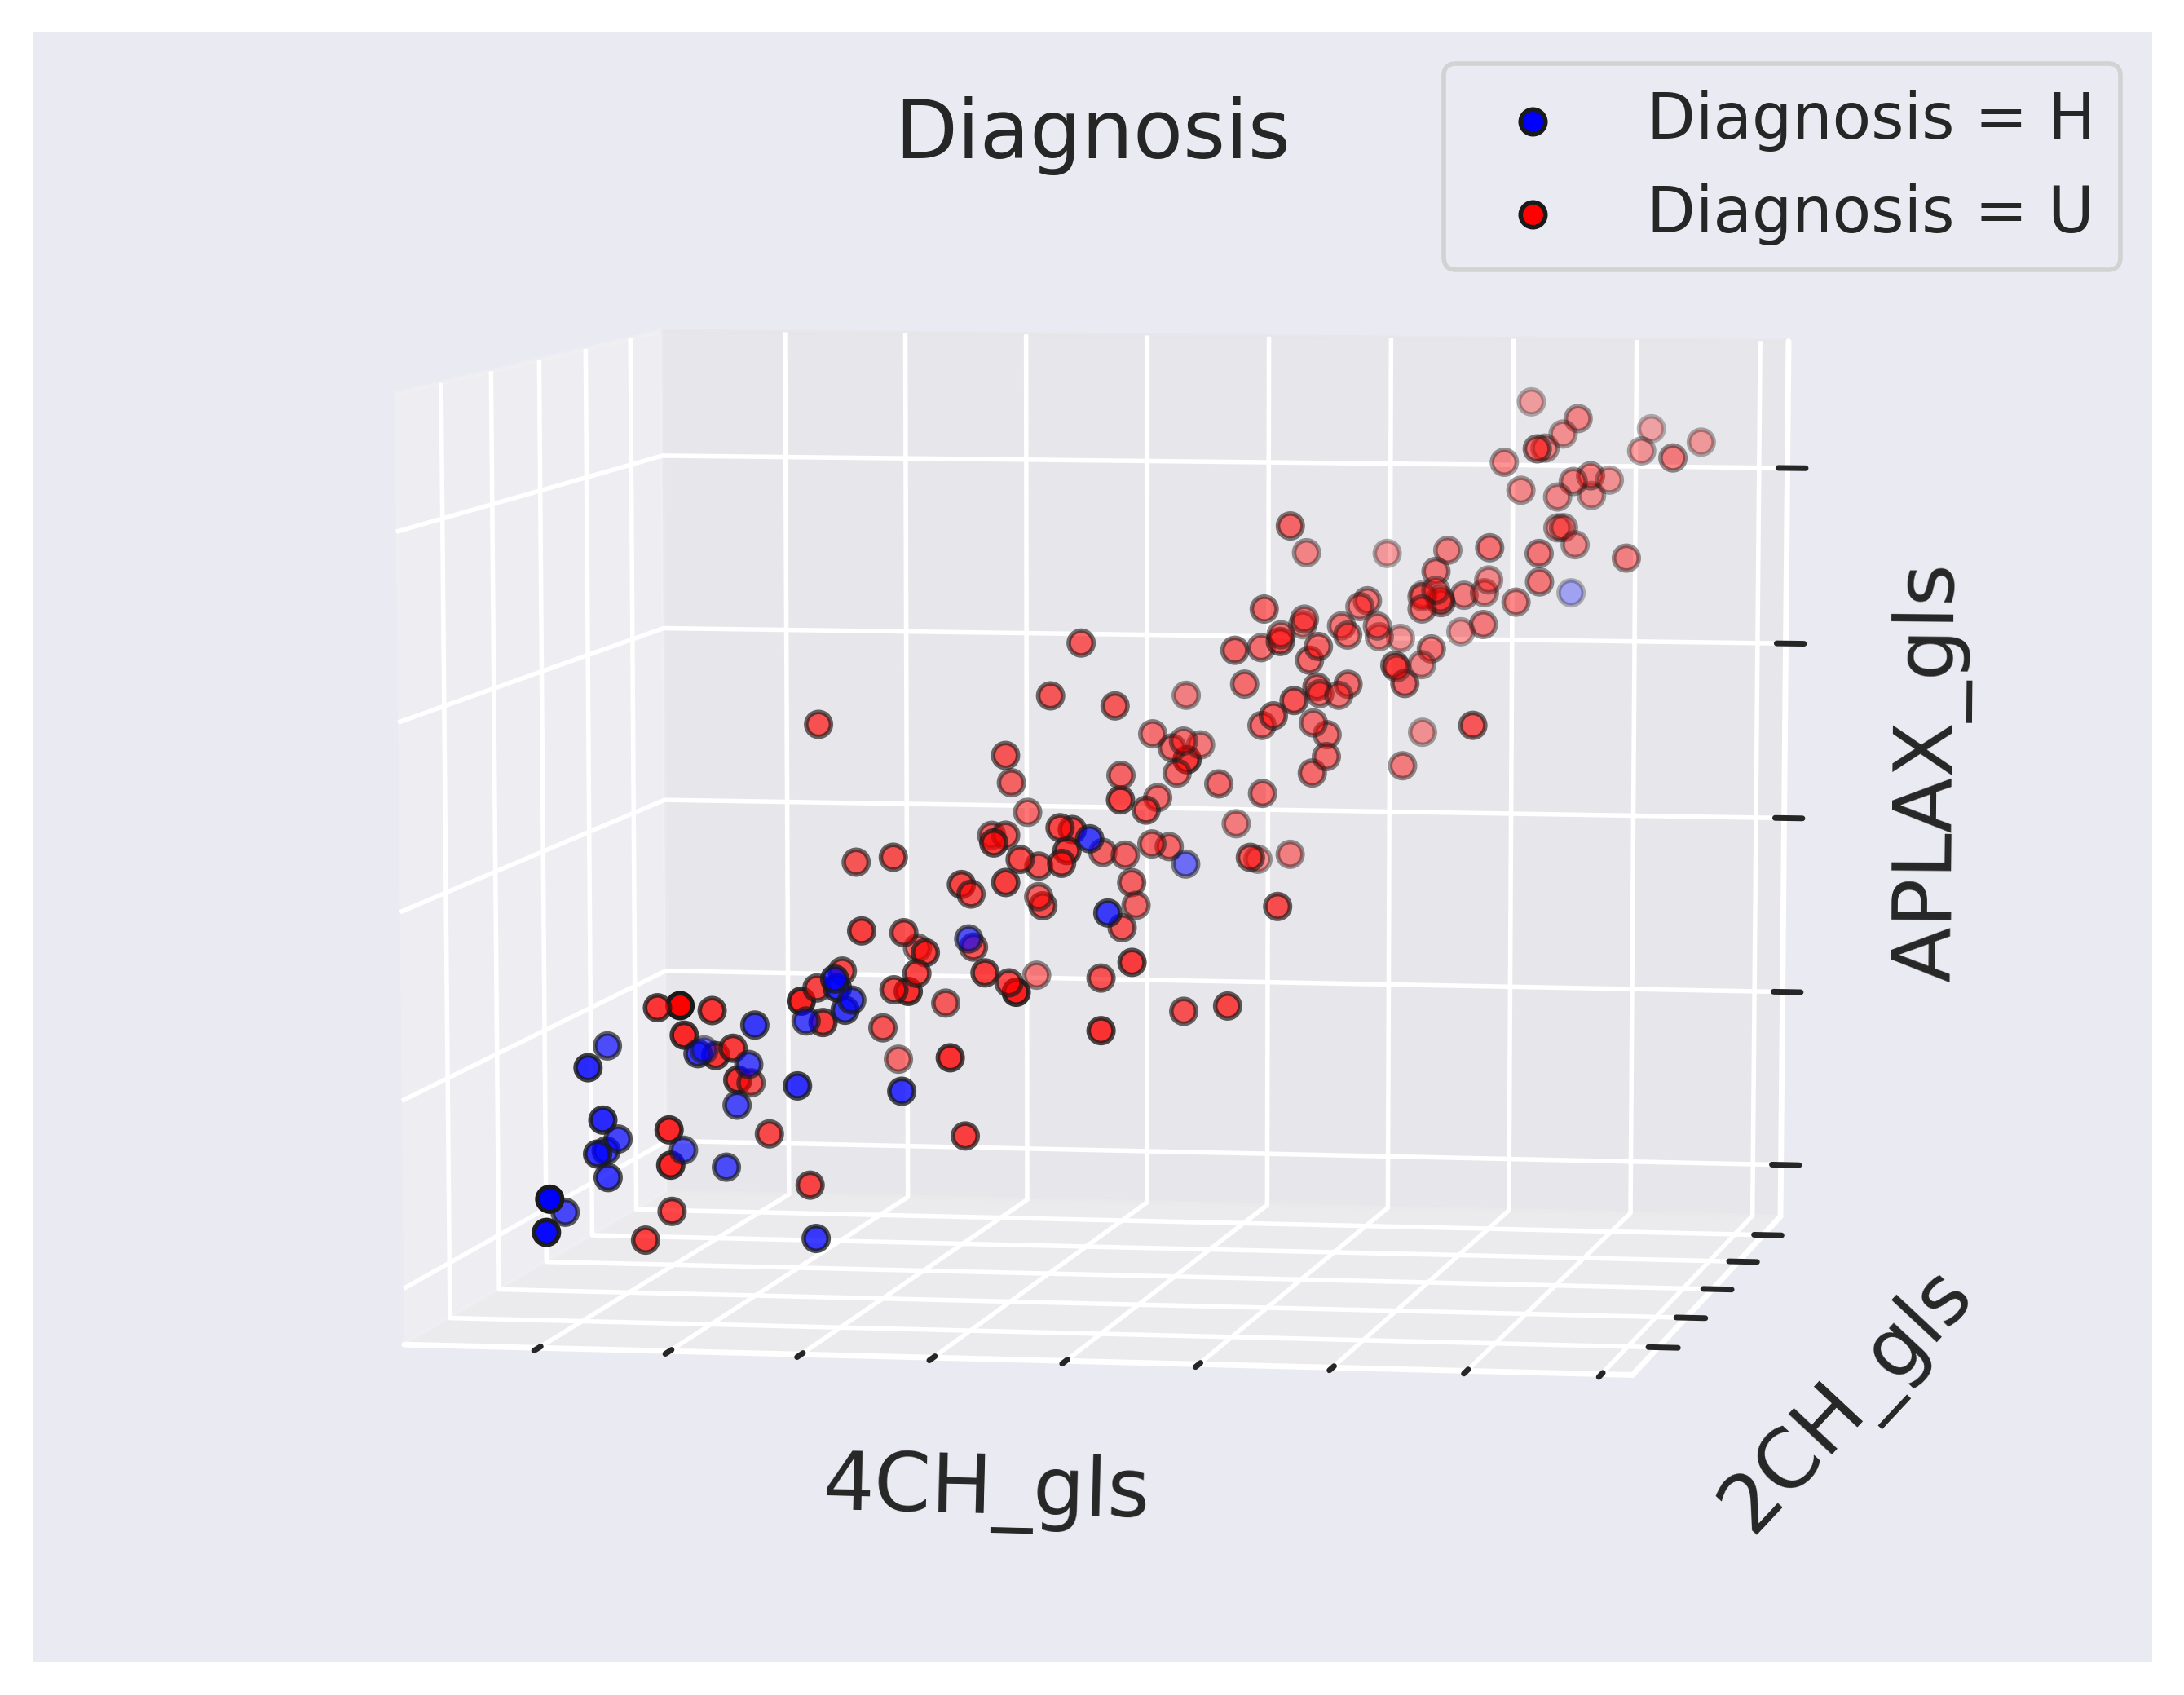
\includegraphics[width=0.99\textwidth]{results/pd/scatter_gls_indication_bin.png}
        \caption{Patient Diagnosis. \textbf{H} stands for \textbf{Healthy}, and \textbf{U} stands for \textbf{Unhealthy}}
        \label{fig:scatter_gls_pd}
    \end{subfigure}
    \begin{subfigure}[b]{0.49\textwidth}
        \centering
        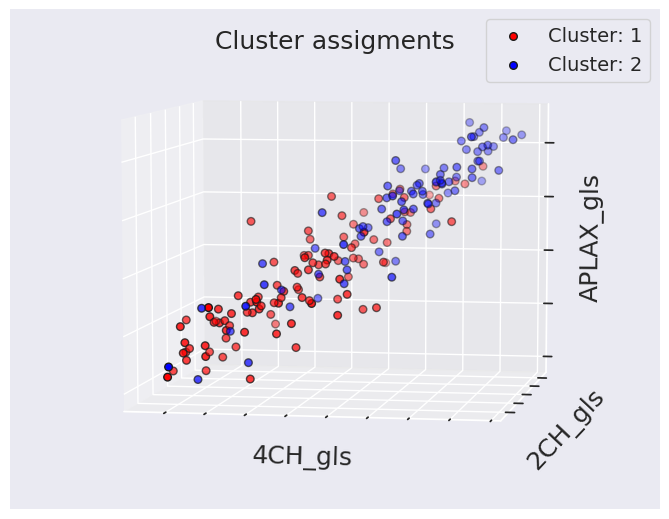
\includegraphics[width=0.99\textwidth]{results/pd/scatter_gls_EF_ward2.png}
        \caption{\textit{GLS-EF Ward/2} cluster assignments.}
        \label{fig:scatter_gls_ef_ward2_ind}
    \end{subfigure}\\
    \begin{subfigure}[b]{0.49\textwidth}
        \centering
        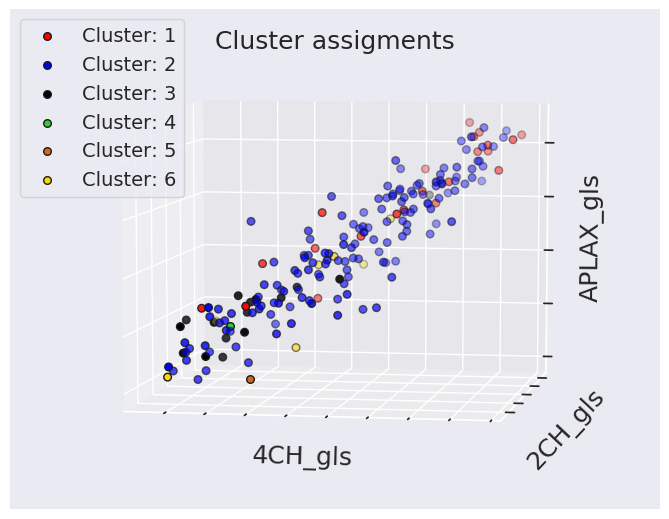
\includegraphics[width=0.99\textwidth]{results/pd/scatter_gls_average6.png}
        \caption{\textit{GLS Average/6} cluster assignments.}
        \label{fig:scatter_gls_average6}
    \end{subfigure}
    \begin{subfigure}[b]{0.49\textwidth}
        \centering
        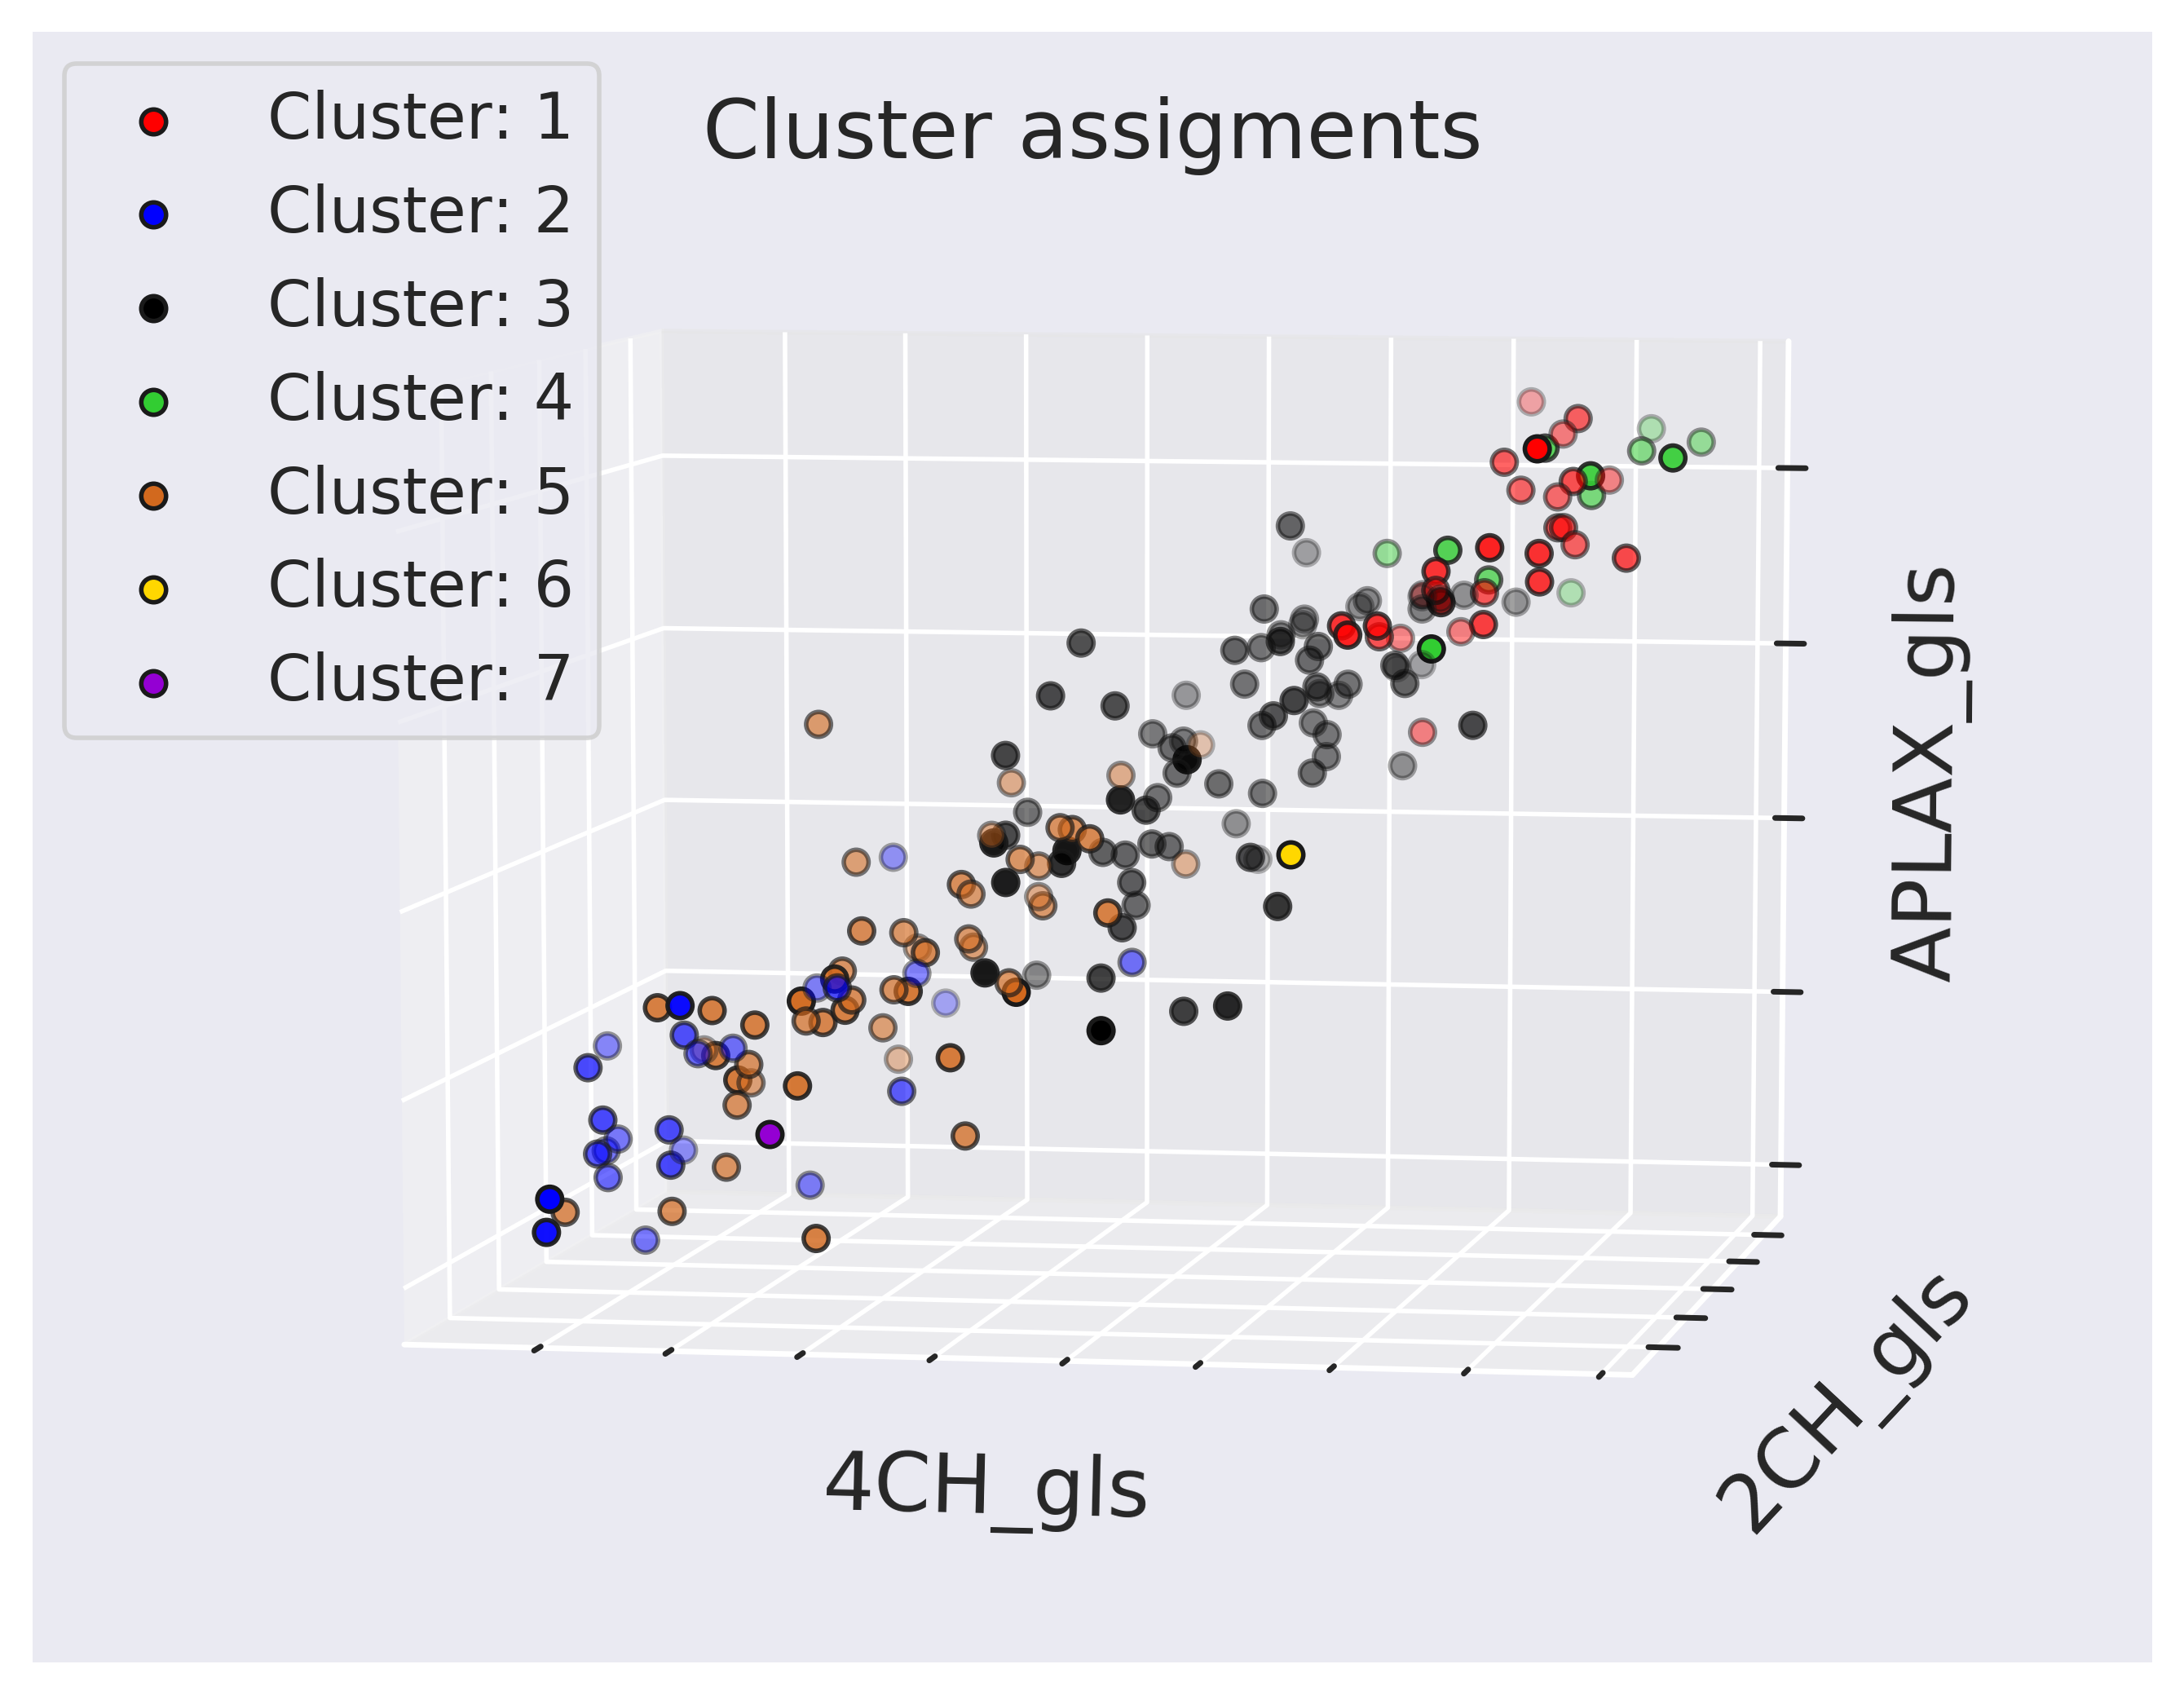
\includegraphics[width=0.99\textwidth]{results/pd/scatter_gls_average7.png}
        \caption{\textit{GLS Average/7} cluster assignments.}
        \label{fig:scatter_gls_average7}
    \end{subfigure}
    \caption{Scatterplot of peak GLS values in each view. Colors in the of the different dots are given by heart failure diagnosis, and cluster assignments of 
             \textit{gls-EF/ward/2}, \textit{average/6} and \textit{average/7} methods. Numbers are not included on the axes because the point of the figure is to illustrate the separability 
             of clusters, and patient diagnosis.}
             \label{fig:scatter_gls_ind_cluster_assignments}
\end{figure}

\newpage

\subsection{Deep Neural Network}

\begin{figure}[H]
    \centering
    %% Creator: Matplotlib, PGF backend
%%
%% To include the figure in your LaTeX document, write
%%   \input{<filename>.pgf}
%%
%% Make sure the required packages are loaded in your preamble
%%   \usepackage{pgf}
%%
%% Figures using additional raster images can only be included by \input if
%% they are in the same directory as the main LaTeX file. For loading figures
%% from other directories you can use the `import` package
%%   \usepackage{import}
%% and then include the figures with
%%   \import{<path to file>}{<filename>.pgf}
%%
%% Matplotlib used the following preamble
%%
\begingroup%
\makeatletter%
\begin{pgfpicture}%
\pgfpathrectangle{\pgfpointorigin}{\pgfqpoint{6.439273in}{2.540000in}}%
\pgfusepath{use as bounding box, clip}%
\begin{pgfscope}%
\pgfsetbuttcap%
\pgfsetmiterjoin%
\definecolor{currentfill}{rgb}{1.000000,1.000000,1.000000}%
\pgfsetfillcolor{currentfill}%
\pgfsetlinewidth{0.000000pt}%
\definecolor{currentstroke}{rgb}{1.000000,1.000000,1.000000}%
\pgfsetstrokecolor{currentstroke}%
\pgfsetdash{}{0pt}%
\pgfpathmoveto{\pgfqpoint{0.000000in}{0.000000in}}%
\pgfpathlineto{\pgfqpoint{6.439273in}{0.000000in}}%
\pgfpathlineto{\pgfqpoint{6.439273in}{2.540000in}}%
\pgfpathlineto{\pgfqpoint{0.000000in}{2.540000in}}%
\pgfpathclose%
\pgfusepath{fill}%
\end{pgfscope}%
\begin{pgfscope}%
\pgfsetbuttcap%
\pgfsetmiterjoin%
\definecolor{currentfill}{rgb}{0.917647,0.917647,0.949020}%
\pgfsetfillcolor{currentfill}%
\pgfsetlinewidth{0.000000pt}%
\definecolor{currentstroke}{rgb}{0.000000,0.000000,0.000000}%
\pgfsetstrokecolor{currentstroke}%
\pgfsetstrokeopacity{0.000000}%
\pgfsetdash{}{0pt}%
\pgfpathmoveto{\pgfqpoint{0.693056in}{0.557870in}}%
\pgfpathlineto{\pgfqpoint{3.156042in}{0.557870in}}%
\pgfpathlineto{\pgfqpoint{3.156042in}{2.242604in}}%
\pgfpathlineto{\pgfqpoint{0.693056in}{2.242604in}}%
\pgfpathclose%
\pgfusepath{fill}%
\end{pgfscope}%
\begin{pgfscope}%
\pgfpathrectangle{\pgfqpoint{0.693056in}{0.557870in}}{\pgfqpoint{2.462986in}{1.684734in}}%
\pgfusepath{clip}%
\pgfsetroundcap%
\pgfsetroundjoin%
\pgfsetlinewidth{1.003750pt}%
\definecolor{currentstroke}{rgb}{1.000000,1.000000,1.000000}%
\pgfsetstrokecolor{currentstroke}%
\pgfsetdash{}{0pt}%
\pgfpathmoveto{\pgfqpoint{0.805010in}{0.557870in}}%
\pgfpathlineto{\pgfqpoint{0.805010in}{2.242604in}}%
\pgfusepath{stroke}%
\end{pgfscope}%
\begin{pgfscope}%
\definecolor{textcolor}{rgb}{0.150000,0.150000,0.150000}%
\pgfsetstrokecolor{textcolor}%
\pgfsetfillcolor{textcolor}%
\pgftext[x=0.805010in,y=0.425926in,,top]{\color{textcolor}\sffamily\fontsize{11.000000}{13.200000}\selectfont \(\displaystyle -0.50\)}%
\end{pgfscope}%
\begin{pgfscope}%
\pgfpathrectangle{\pgfqpoint{0.693056in}{0.557870in}}{\pgfqpoint{2.462986in}{1.684734in}}%
\pgfusepath{clip}%
\pgfsetroundcap%
\pgfsetroundjoin%
\pgfsetlinewidth{1.003750pt}%
\definecolor{currentstroke}{rgb}{1.000000,1.000000,1.000000}%
\pgfsetstrokecolor{currentstroke}%
\pgfsetdash{}{0pt}%
\pgfpathmoveto{\pgfqpoint{1.364779in}{0.557870in}}%
\pgfpathlineto{\pgfqpoint{1.364779in}{2.242604in}}%
\pgfusepath{stroke}%
\end{pgfscope}%
\begin{pgfscope}%
\definecolor{textcolor}{rgb}{0.150000,0.150000,0.150000}%
\pgfsetstrokecolor{textcolor}%
\pgfsetfillcolor{textcolor}%
\pgftext[x=1.364779in,y=0.425926in,,top]{\color{textcolor}\sffamily\fontsize{11.000000}{13.200000}\selectfont \(\displaystyle -0.25\)}%
\end{pgfscope}%
\begin{pgfscope}%
\pgfpathrectangle{\pgfqpoint{0.693056in}{0.557870in}}{\pgfqpoint{2.462986in}{1.684734in}}%
\pgfusepath{clip}%
\pgfsetroundcap%
\pgfsetroundjoin%
\pgfsetlinewidth{1.003750pt}%
\definecolor{currentstroke}{rgb}{1.000000,1.000000,1.000000}%
\pgfsetstrokecolor{currentstroke}%
\pgfsetdash{}{0pt}%
\pgfpathmoveto{\pgfqpoint{1.924549in}{0.557870in}}%
\pgfpathlineto{\pgfqpoint{1.924549in}{2.242604in}}%
\pgfusepath{stroke}%
\end{pgfscope}%
\begin{pgfscope}%
\definecolor{textcolor}{rgb}{0.150000,0.150000,0.150000}%
\pgfsetstrokecolor{textcolor}%
\pgfsetfillcolor{textcolor}%
\pgftext[x=1.924549in,y=0.425926in,,top]{\color{textcolor}\sffamily\fontsize{11.000000}{13.200000}\selectfont \(\displaystyle 0.00\)}%
\end{pgfscope}%
\begin{pgfscope}%
\pgfpathrectangle{\pgfqpoint{0.693056in}{0.557870in}}{\pgfqpoint{2.462986in}{1.684734in}}%
\pgfusepath{clip}%
\pgfsetroundcap%
\pgfsetroundjoin%
\pgfsetlinewidth{1.003750pt}%
\definecolor{currentstroke}{rgb}{1.000000,1.000000,1.000000}%
\pgfsetstrokecolor{currentstroke}%
\pgfsetdash{}{0pt}%
\pgfpathmoveto{\pgfqpoint{2.484318in}{0.557870in}}%
\pgfpathlineto{\pgfqpoint{2.484318in}{2.242604in}}%
\pgfusepath{stroke}%
\end{pgfscope}%
\begin{pgfscope}%
\definecolor{textcolor}{rgb}{0.150000,0.150000,0.150000}%
\pgfsetstrokecolor{textcolor}%
\pgfsetfillcolor{textcolor}%
\pgftext[x=2.484318in,y=0.425926in,,top]{\color{textcolor}\sffamily\fontsize{11.000000}{13.200000}\selectfont \(\displaystyle 0.25\)}%
\end{pgfscope}%
\begin{pgfscope}%
\pgfpathrectangle{\pgfqpoint{0.693056in}{0.557870in}}{\pgfqpoint{2.462986in}{1.684734in}}%
\pgfusepath{clip}%
\pgfsetroundcap%
\pgfsetroundjoin%
\pgfsetlinewidth{1.003750pt}%
\definecolor{currentstroke}{rgb}{1.000000,1.000000,1.000000}%
\pgfsetstrokecolor{currentstroke}%
\pgfsetdash{}{0pt}%
\pgfpathmoveto{\pgfqpoint{3.044088in}{0.557870in}}%
\pgfpathlineto{\pgfqpoint{3.044088in}{2.242604in}}%
\pgfusepath{stroke}%
\end{pgfscope}%
\begin{pgfscope}%
\definecolor{textcolor}{rgb}{0.150000,0.150000,0.150000}%
\pgfsetstrokecolor{textcolor}%
\pgfsetfillcolor{textcolor}%
\pgftext[x=3.044088in,y=0.425926in,,top]{\color{textcolor}\sffamily\fontsize{11.000000}{13.200000}\selectfont \(\displaystyle 0.50\)}%
\end{pgfscope}%
\begin{pgfscope}%
\definecolor{textcolor}{rgb}{0.150000,0.150000,0.150000}%
\pgfsetstrokecolor{textcolor}%
\pgfsetfillcolor{textcolor}%
\pgftext[x=1.924549in,y=0.235185in,,top]{\color{textcolor}\sffamily\fontsize{11.000000}{13.200000}\selectfont DOR}%
\end{pgfscope}%
\begin{pgfscope}%
\pgfpathrectangle{\pgfqpoint{0.693056in}{0.557870in}}{\pgfqpoint{2.462986in}{1.684734in}}%
\pgfusepath{clip}%
\pgfsetroundcap%
\pgfsetroundjoin%
\pgfsetlinewidth{1.003750pt}%
\definecolor{currentstroke}{rgb}{1.000000,1.000000,1.000000}%
\pgfsetstrokecolor{currentstroke}%
\pgfsetdash{}{0pt}%
\pgfpathmoveto{\pgfqpoint{0.693056in}{0.557870in}}%
\pgfpathlineto{\pgfqpoint{3.156042in}{0.557870in}}%
\pgfusepath{stroke}%
\end{pgfscope}%
\begin{pgfscope}%
\definecolor{textcolor}{rgb}{0.150000,0.150000,0.150000}%
\pgfsetstrokecolor{textcolor}%
\pgfsetfillcolor{textcolor}%
\pgftext[x=0.290741in,y=0.505064in,left,base]{\color{textcolor}\sffamily\fontsize{11.000000}{13.200000}\selectfont \(\displaystyle 0.00\)}%
\end{pgfscope}%
\begin{pgfscope}%
\pgfpathrectangle{\pgfqpoint{0.693056in}{0.557870in}}{\pgfqpoint{2.462986in}{1.684734in}}%
\pgfusepath{clip}%
\pgfsetroundcap%
\pgfsetroundjoin%
\pgfsetlinewidth{1.003750pt}%
\definecolor{currentstroke}{rgb}{1.000000,1.000000,1.000000}%
\pgfsetstrokecolor{currentstroke}%
\pgfsetdash{}{0pt}%
\pgfpathmoveto{\pgfqpoint{0.693056in}{0.958997in}}%
\pgfpathlineto{\pgfqpoint{3.156042in}{0.958997in}}%
\pgfusepath{stroke}%
\end{pgfscope}%
\begin{pgfscope}%
\definecolor{textcolor}{rgb}{0.150000,0.150000,0.150000}%
\pgfsetstrokecolor{textcolor}%
\pgfsetfillcolor{textcolor}%
\pgftext[x=0.290741in,y=0.906191in,left,base]{\color{textcolor}\sffamily\fontsize{11.000000}{13.200000}\selectfont \(\displaystyle 0.25\)}%
\end{pgfscope}%
\begin{pgfscope}%
\pgfpathrectangle{\pgfqpoint{0.693056in}{0.557870in}}{\pgfqpoint{2.462986in}{1.684734in}}%
\pgfusepath{clip}%
\pgfsetroundcap%
\pgfsetroundjoin%
\pgfsetlinewidth{1.003750pt}%
\definecolor{currentstroke}{rgb}{1.000000,1.000000,1.000000}%
\pgfsetstrokecolor{currentstroke}%
\pgfsetdash{}{0pt}%
\pgfpathmoveto{\pgfqpoint{0.693056in}{1.360125in}}%
\pgfpathlineto{\pgfqpoint{3.156042in}{1.360125in}}%
\pgfusepath{stroke}%
\end{pgfscope}%
\begin{pgfscope}%
\definecolor{textcolor}{rgb}{0.150000,0.150000,0.150000}%
\pgfsetstrokecolor{textcolor}%
\pgfsetfillcolor{textcolor}%
\pgftext[x=0.290741in,y=1.307318in,left,base]{\color{textcolor}\sffamily\fontsize{11.000000}{13.200000}\selectfont \(\displaystyle 0.50\)}%
\end{pgfscope}%
\begin{pgfscope}%
\pgfpathrectangle{\pgfqpoint{0.693056in}{0.557870in}}{\pgfqpoint{2.462986in}{1.684734in}}%
\pgfusepath{clip}%
\pgfsetroundcap%
\pgfsetroundjoin%
\pgfsetlinewidth{1.003750pt}%
\definecolor{currentstroke}{rgb}{1.000000,1.000000,1.000000}%
\pgfsetstrokecolor{currentstroke}%
\pgfsetdash{}{0pt}%
\pgfpathmoveto{\pgfqpoint{0.693056in}{1.761252in}}%
\pgfpathlineto{\pgfqpoint{3.156042in}{1.761252in}}%
\pgfusepath{stroke}%
\end{pgfscope}%
\begin{pgfscope}%
\definecolor{textcolor}{rgb}{0.150000,0.150000,0.150000}%
\pgfsetstrokecolor{textcolor}%
\pgfsetfillcolor{textcolor}%
\pgftext[x=0.290741in,y=1.708445in,left,base]{\color{textcolor}\sffamily\fontsize{11.000000}{13.200000}\selectfont \(\displaystyle 0.75\)}%
\end{pgfscope}%
\begin{pgfscope}%
\pgfpathrectangle{\pgfqpoint{0.693056in}{0.557870in}}{\pgfqpoint{2.462986in}{1.684734in}}%
\pgfusepath{clip}%
\pgfsetroundcap%
\pgfsetroundjoin%
\pgfsetlinewidth{1.003750pt}%
\definecolor{currentstroke}{rgb}{1.000000,1.000000,1.000000}%
\pgfsetstrokecolor{currentstroke}%
\pgfsetdash{}{0pt}%
\pgfpathmoveto{\pgfqpoint{0.693056in}{2.162379in}}%
\pgfpathlineto{\pgfqpoint{3.156042in}{2.162379in}}%
\pgfusepath{stroke}%
\end{pgfscope}%
\begin{pgfscope}%
\definecolor{textcolor}{rgb}{0.150000,0.150000,0.150000}%
\pgfsetstrokecolor{textcolor}%
\pgfsetfillcolor{textcolor}%
\pgftext[x=0.290741in,y=2.109572in,left,base]{\color{textcolor}\sffamily\fontsize{11.000000}{13.200000}\selectfont \(\displaystyle 1.00\)}%
\end{pgfscope}%
\begin{pgfscope}%
\definecolor{textcolor}{rgb}{0.150000,0.150000,0.150000}%
\pgfsetstrokecolor{textcolor}%
\pgfsetfillcolor{textcolor}%
\pgftext[x=0.235185in,y=1.400237in,,bottom,rotate=90.000000]{\color{textcolor}\sffamily\fontsize{11.000000}{13.200000}\selectfont Occurance}%
\end{pgfscope}%
\begin{pgfscope}%
\pgfpathrectangle{\pgfqpoint{0.693056in}{0.557870in}}{\pgfqpoint{2.462986in}{1.684734in}}%
\pgfusepath{clip}%
\pgfsetbuttcap%
\pgfsetmiterjoin%
\definecolor{currentfill}{rgb}{0.298039,0.447059,0.690196}%
\pgfsetfillcolor{currentfill}%
\pgfsetfillopacity{0.400000}%
\pgfsetlinewidth{1.003750pt}%
\definecolor{currentstroke}{rgb}{1.000000,1.000000,1.000000}%
\pgfsetstrokecolor{currentstroke}%
\pgfsetstrokeopacity{0.400000}%
\pgfsetdash{}{0pt}%
\pgfpathmoveto{\pgfqpoint{0.805010in}{0.557870in}}%
\pgfpathlineto{\pgfqpoint{1.028918in}{0.557870in}}%
\pgfpathlineto{\pgfqpoint{1.028918in}{0.557870in}}%
\pgfpathlineto{\pgfqpoint{0.805010in}{0.557870in}}%
\pgfpathclose%
\pgfusepath{stroke,fill}%
\end{pgfscope}%
\begin{pgfscope}%
\pgfpathrectangle{\pgfqpoint{0.693056in}{0.557870in}}{\pgfqpoint{2.462986in}{1.684734in}}%
\pgfusepath{clip}%
\pgfsetbuttcap%
\pgfsetmiterjoin%
\definecolor{currentfill}{rgb}{0.298039,0.447059,0.690196}%
\pgfsetfillcolor{currentfill}%
\pgfsetfillopacity{0.400000}%
\pgfsetlinewidth{1.003750pt}%
\definecolor{currentstroke}{rgb}{1.000000,1.000000,1.000000}%
\pgfsetstrokecolor{currentstroke}%
\pgfsetstrokeopacity{0.400000}%
\pgfsetdash{}{0pt}%
\pgfpathmoveto{\pgfqpoint{1.028918in}{0.557870in}}%
\pgfpathlineto{\pgfqpoint{1.252825in}{0.557870in}}%
\pgfpathlineto{\pgfqpoint{1.252825in}{0.557870in}}%
\pgfpathlineto{\pgfqpoint{1.028918in}{0.557870in}}%
\pgfpathclose%
\pgfusepath{stroke,fill}%
\end{pgfscope}%
\begin{pgfscope}%
\pgfpathrectangle{\pgfqpoint{0.693056in}{0.557870in}}{\pgfqpoint{2.462986in}{1.684734in}}%
\pgfusepath{clip}%
\pgfsetbuttcap%
\pgfsetmiterjoin%
\definecolor{currentfill}{rgb}{0.298039,0.447059,0.690196}%
\pgfsetfillcolor{currentfill}%
\pgfsetfillopacity{0.400000}%
\pgfsetlinewidth{1.003750pt}%
\definecolor{currentstroke}{rgb}{1.000000,1.000000,1.000000}%
\pgfsetstrokecolor{currentstroke}%
\pgfsetstrokeopacity{0.400000}%
\pgfsetdash{}{0pt}%
\pgfpathmoveto{\pgfqpoint{1.252825in}{0.557870in}}%
\pgfpathlineto{\pgfqpoint{1.476733in}{0.557870in}}%
\pgfpathlineto{\pgfqpoint{1.476733in}{0.557870in}}%
\pgfpathlineto{\pgfqpoint{1.252825in}{0.557870in}}%
\pgfpathclose%
\pgfusepath{stroke,fill}%
\end{pgfscope}%
\begin{pgfscope}%
\pgfpathrectangle{\pgfqpoint{0.693056in}{0.557870in}}{\pgfqpoint{2.462986in}{1.684734in}}%
\pgfusepath{clip}%
\pgfsetbuttcap%
\pgfsetmiterjoin%
\definecolor{currentfill}{rgb}{0.298039,0.447059,0.690196}%
\pgfsetfillcolor{currentfill}%
\pgfsetfillopacity{0.400000}%
\pgfsetlinewidth{1.003750pt}%
\definecolor{currentstroke}{rgb}{1.000000,1.000000,1.000000}%
\pgfsetstrokecolor{currentstroke}%
\pgfsetstrokeopacity{0.400000}%
\pgfsetdash{}{0pt}%
\pgfpathmoveto{\pgfqpoint{1.476733in}{0.557870in}}%
\pgfpathlineto{\pgfqpoint{1.700641in}{0.557870in}}%
\pgfpathlineto{\pgfqpoint{1.700641in}{0.557870in}}%
\pgfpathlineto{\pgfqpoint{1.476733in}{0.557870in}}%
\pgfpathclose%
\pgfusepath{stroke,fill}%
\end{pgfscope}%
\begin{pgfscope}%
\pgfpathrectangle{\pgfqpoint{0.693056in}{0.557870in}}{\pgfqpoint{2.462986in}{1.684734in}}%
\pgfusepath{clip}%
\pgfsetbuttcap%
\pgfsetmiterjoin%
\definecolor{currentfill}{rgb}{0.298039,0.447059,0.690196}%
\pgfsetfillcolor{currentfill}%
\pgfsetfillopacity{0.400000}%
\pgfsetlinewidth{1.003750pt}%
\definecolor{currentstroke}{rgb}{1.000000,1.000000,1.000000}%
\pgfsetstrokecolor{currentstroke}%
\pgfsetstrokeopacity{0.400000}%
\pgfsetdash{}{0pt}%
\pgfpathmoveto{\pgfqpoint{1.700641in}{0.557870in}}%
\pgfpathlineto{\pgfqpoint{1.924549in}{0.557870in}}%
\pgfpathlineto{\pgfqpoint{1.924549in}{0.557870in}}%
\pgfpathlineto{\pgfqpoint{1.700641in}{0.557870in}}%
\pgfpathclose%
\pgfusepath{stroke,fill}%
\end{pgfscope}%
\begin{pgfscope}%
\pgfpathrectangle{\pgfqpoint{0.693056in}{0.557870in}}{\pgfqpoint{2.462986in}{1.684734in}}%
\pgfusepath{clip}%
\pgfsetbuttcap%
\pgfsetmiterjoin%
\definecolor{currentfill}{rgb}{0.298039,0.447059,0.690196}%
\pgfsetfillcolor{currentfill}%
\pgfsetfillopacity{0.400000}%
\pgfsetlinewidth{1.003750pt}%
\definecolor{currentstroke}{rgb}{1.000000,1.000000,1.000000}%
\pgfsetstrokecolor{currentstroke}%
\pgfsetstrokeopacity{0.400000}%
\pgfsetdash{}{0pt}%
\pgfpathmoveto{\pgfqpoint{1.924549in}{0.557870in}}%
\pgfpathlineto{\pgfqpoint{2.148457in}{0.557870in}}%
\pgfpathlineto{\pgfqpoint{2.148457in}{2.162379in}}%
\pgfpathlineto{\pgfqpoint{1.924549in}{2.162379in}}%
\pgfpathclose%
\pgfusepath{stroke,fill}%
\end{pgfscope}%
\begin{pgfscope}%
\pgfpathrectangle{\pgfqpoint{0.693056in}{0.557870in}}{\pgfqpoint{2.462986in}{1.684734in}}%
\pgfusepath{clip}%
\pgfsetbuttcap%
\pgfsetmiterjoin%
\definecolor{currentfill}{rgb}{0.298039,0.447059,0.690196}%
\pgfsetfillcolor{currentfill}%
\pgfsetfillopacity{0.400000}%
\pgfsetlinewidth{1.003750pt}%
\definecolor{currentstroke}{rgb}{1.000000,1.000000,1.000000}%
\pgfsetstrokecolor{currentstroke}%
\pgfsetstrokeopacity{0.400000}%
\pgfsetdash{}{0pt}%
\pgfpathmoveto{\pgfqpoint{2.148457in}{0.557870in}}%
\pgfpathlineto{\pgfqpoint{2.372364in}{0.557870in}}%
\pgfpathlineto{\pgfqpoint{2.372364in}{0.557870in}}%
\pgfpathlineto{\pgfqpoint{2.148457in}{0.557870in}}%
\pgfpathclose%
\pgfusepath{stroke,fill}%
\end{pgfscope}%
\begin{pgfscope}%
\pgfpathrectangle{\pgfqpoint{0.693056in}{0.557870in}}{\pgfqpoint{2.462986in}{1.684734in}}%
\pgfusepath{clip}%
\pgfsetbuttcap%
\pgfsetmiterjoin%
\definecolor{currentfill}{rgb}{0.298039,0.447059,0.690196}%
\pgfsetfillcolor{currentfill}%
\pgfsetfillopacity{0.400000}%
\pgfsetlinewidth{1.003750pt}%
\definecolor{currentstroke}{rgb}{1.000000,1.000000,1.000000}%
\pgfsetstrokecolor{currentstroke}%
\pgfsetstrokeopacity{0.400000}%
\pgfsetdash{}{0pt}%
\pgfpathmoveto{\pgfqpoint{2.372364in}{0.557870in}}%
\pgfpathlineto{\pgfqpoint{2.596272in}{0.557870in}}%
\pgfpathlineto{\pgfqpoint{2.596272in}{0.557870in}}%
\pgfpathlineto{\pgfqpoint{2.372364in}{0.557870in}}%
\pgfpathclose%
\pgfusepath{stroke,fill}%
\end{pgfscope}%
\begin{pgfscope}%
\pgfpathrectangle{\pgfqpoint{0.693056in}{0.557870in}}{\pgfqpoint{2.462986in}{1.684734in}}%
\pgfusepath{clip}%
\pgfsetbuttcap%
\pgfsetmiterjoin%
\definecolor{currentfill}{rgb}{0.298039,0.447059,0.690196}%
\pgfsetfillcolor{currentfill}%
\pgfsetfillopacity{0.400000}%
\pgfsetlinewidth{1.003750pt}%
\definecolor{currentstroke}{rgb}{1.000000,1.000000,1.000000}%
\pgfsetstrokecolor{currentstroke}%
\pgfsetstrokeopacity{0.400000}%
\pgfsetdash{}{0pt}%
\pgfpathmoveto{\pgfqpoint{2.596272in}{0.557870in}}%
\pgfpathlineto{\pgfqpoint{2.820180in}{0.557870in}}%
\pgfpathlineto{\pgfqpoint{2.820180in}{0.557870in}}%
\pgfpathlineto{\pgfqpoint{2.596272in}{0.557870in}}%
\pgfpathclose%
\pgfusepath{stroke,fill}%
\end{pgfscope}%
\begin{pgfscope}%
\pgfpathrectangle{\pgfqpoint{0.693056in}{0.557870in}}{\pgfqpoint{2.462986in}{1.684734in}}%
\pgfusepath{clip}%
\pgfsetbuttcap%
\pgfsetmiterjoin%
\definecolor{currentfill}{rgb}{0.298039,0.447059,0.690196}%
\pgfsetfillcolor{currentfill}%
\pgfsetfillopacity{0.400000}%
\pgfsetlinewidth{1.003750pt}%
\definecolor{currentstroke}{rgb}{1.000000,1.000000,1.000000}%
\pgfsetstrokecolor{currentstroke}%
\pgfsetstrokeopacity{0.400000}%
\pgfsetdash{}{0pt}%
\pgfpathmoveto{\pgfqpoint{2.820180in}{0.557870in}}%
\pgfpathlineto{\pgfqpoint{3.044088in}{0.557870in}}%
\pgfpathlineto{\pgfqpoint{3.044088in}{0.557870in}}%
\pgfpathlineto{\pgfqpoint{2.820180in}{0.557870in}}%
\pgfpathclose%
\pgfusepath{stroke,fill}%
\end{pgfscope}%
\begin{pgfscope}%
\pgfsetrectcap%
\pgfsetmiterjoin%
\pgfsetlinewidth{1.254687pt}%
\definecolor{currentstroke}{rgb}{1.000000,1.000000,1.000000}%
\pgfsetstrokecolor{currentstroke}%
\pgfsetdash{}{0pt}%
\pgfpathmoveto{\pgfqpoint{0.693056in}{0.557870in}}%
\pgfpathlineto{\pgfqpoint{0.693056in}{2.242604in}}%
\pgfusepath{stroke}%
\end{pgfscope}%
\begin{pgfscope}%
\pgfsetrectcap%
\pgfsetmiterjoin%
\pgfsetlinewidth{1.254687pt}%
\definecolor{currentstroke}{rgb}{1.000000,1.000000,1.000000}%
\pgfsetstrokecolor{currentstroke}%
\pgfsetdash{}{0pt}%
\pgfpathmoveto{\pgfqpoint{3.156042in}{0.557870in}}%
\pgfpathlineto{\pgfqpoint{3.156042in}{2.242604in}}%
\pgfusepath{stroke}%
\end{pgfscope}%
\begin{pgfscope}%
\pgfsetrectcap%
\pgfsetmiterjoin%
\pgfsetlinewidth{1.254687pt}%
\definecolor{currentstroke}{rgb}{1.000000,1.000000,1.000000}%
\pgfsetstrokecolor{currentstroke}%
\pgfsetdash{}{0pt}%
\pgfpathmoveto{\pgfqpoint{0.693056in}{0.557870in}}%
\pgfpathlineto{\pgfqpoint{3.156042in}{0.557870in}}%
\pgfusepath{stroke}%
\end{pgfscope}%
\begin{pgfscope}%
\pgfsetrectcap%
\pgfsetmiterjoin%
\pgfsetlinewidth{1.254687pt}%
\definecolor{currentstroke}{rgb}{1.000000,1.000000,1.000000}%
\pgfsetstrokecolor{currentstroke}%
\pgfsetdash{}{0pt}%
\pgfpathmoveto{\pgfqpoint{0.693056in}{2.242604in}}%
\pgfpathlineto{\pgfqpoint{3.156042in}{2.242604in}}%
\pgfusepath{stroke}%
\end{pgfscope}%
\begin{pgfscope}%
\definecolor{textcolor}{rgb}{0.150000,0.150000,0.150000}%
\pgfsetstrokecolor{textcolor}%
\pgfsetfillcolor{textcolor}%
\pgftext[x=1.924549in,y=2.325938in,,base]{\color{textcolor}\sffamily\fontsize{11.000000}{13.200000}\selectfont (a)}%
\end{pgfscope}%
\begin{pgfscope}%
\pgfsetbuttcap%
\pgfsetmiterjoin%
\definecolor{currentfill}{rgb}{0.917647,0.917647,0.949020}%
\pgfsetfillcolor{currentfill}%
\pgfsetlinewidth{0.000000pt}%
\definecolor{currentstroke}{rgb}{0.000000,0.000000,0.000000}%
\pgfsetstrokecolor{currentstroke}%
\pgfsetstrokeopacity{0.000000}%
\pgfsetdash{}{0pt}%
\pgfpathmoveto{\pgfqpoint{3.853056in}{0.557870in}}%
\pgfpathlineto{\pgfqpoint{6.316042in}{0.557870in}}%
\pgfpathlineto{\pgfqpoint{6.316042in}{2.242604in}}%
\pgfpathlineto{\pgfqpoint{3.853056in}{2.242604in}}%
\pgfpathclose%
\pgfusepath{fill}%
\end{pgfscope}%
\begin{pgfscope}%
\pgfpathrectangle{\pgfqpoint{3.853056in}{0.557870in}}{\pgfqpoint{2.462986in}{1.684734in}}%
\pgfusepath{clip}%
\pgfsetroundcap%
\pgfsetroundjoin%
\pgfsetlinewidth{1.003750pt}%
\definecolor{currentstroke}{rgb}{1.000000,1.000000,1.000000}%
\pgfsetstrokecolor{currentstroke}%
\pgfsetdash{}{0pt}%
\pgfpathmoveto{\pgfqpoint{3.965010in}{0.557870in}}%
\pgfpathlineto{\pgfqpoint{3.965010in}{2.242604in}}%
\pgfusepath{stroke}%
\end{pgfscope}%
\begin{pgfscope}%
\definecolor{textcolor}{rgb}{0.150000,0.150000,0.150000}%
\pgfsetstrokecolor{textcolor}%
\pgfsetfillcolor{textcolor}%
\pgftext[x=3.965010in,y=0.425926in,,top]{\color{textcolor}\sffamily\fontsize{11.000000}{13.200000}\selectfont \(\displaystyle 0.00\)}%
\end{pgfscope}%
\begin{pgfscope}%
\pgfpathrectangle{\pgfqpoint{3.853056in}{0.557870in}}{\pgfqpoint{2.462986in}{1.684734in}}%
\pgfusepath{clip}%
\pgfsetroundcap%
\pgfsetroundjoin%
\pgfsetlinewidth{1.003750pt}%
\definecolor{currentstroke}{rgb}{1.000000,1.000000,1.000000}%
\pgfsetstrokecolor{currentstroke}%
\pgfsetdash{}{0pt}%
\pgfpathmoveto{\pgfqpoint{4.524779in}{0.557870in}}%
\pgfpathlineto{\pgfqpoint{4.524779in}{2.242604in}}%
\pgfusepath{stroke}%
\end{pgfscope}%
\begin{pgfscope}%
\definecolor{textcolor}{rgb}{0.150000,0.150000,0.150000}%
\pgfsetstrokecolor{textcolor}%
\pgfsetfillcolor{textcolor}%
\pgftext[x=4.524779in,y=0.425926in,,top]{\color{textcolor}\sffamily\fontsize{11.000000}{13.200000}\selectfont \(\displaystyle 0.25\)}%
\end{pgfscope}%
\begin{pgfscope}%
\pgfpathrectangle{\pgfqpoint{3.853056in}{0.557870in}}{\pgfqpoint{2.462986in}{1.684734in}}%
\pgfusepath{clip}%
\pgfsetroundcap%
\pgfsetroundjoin%
\pgfsetlinewidth{1.003750pt}%
\definecolor{currentstroke}{rgb}{1.000000,1.000000,1.000000}%
\pgfsetstrokecolor{currentstroke}%
\pgfsetdash{}{0pt}%
\pgfpathmoveto{\pgfqpoint{5.084549in}{0.557870in}}%
\pgfpathlineto{\pgfqpoint{5.084549in}{2.242604in}}%
\pgfusepath{stroke}%
\end{pgfscope}%
\begin{pgfscope}%
\definecolor{textcolor}{rgb}{0.150000,0.150000,0.150000}%
\pgfsetstrokecolor{textcolor}%
\pgfsetfillcolor{textcolor}%
\pgftext[x=5.084549in,y=0.425926in,,top]{\color{textcolor}\sffamily\fontsize{11.000000}{13.200000}\selectfont \(\displaystyle 0.50\)}%
\end{pgfscope}%
\begin{pgfscope}%
\pgfpathrectangle{\pgfqpoint{3.853056in}{0.557870in}}{\pgfqpoint{2.462986in}{1.684734in}}%
\pgfusepath{clip}%
\pgfsetroundcap%
\pgfsetroundjoin%
\pgfsetlinewidth{1.003750pt}%
\definecolor{currentstroke}{rgb}{1.000000,1.000000,1.000000}%
\pgfsetstrokecolor{currentstroke}%
\pgfsetdash{}{0pt}%
\pgfpathmoveto{\pgfqpoint{5.644318in}{0.557870in}}%
\pgfpathlineto{\pgfqpoint{5.644318in}{2.242604in}}%
\pgfusepath{stroke}%
\end{pgfscope}%
\begin{pgfscope}%
\definecolor{textcolor}{rgb}{0.150000,0.150000,0.150000}%
\pgfsetstrokecolor{textcolor}%
\pgfsetfillcolor{textcolor}%
\pgftext[x=5.644318in,y=0.425926in,,top]{\color{textcolor}\sffamily\fontsize{11.000000}{13.200000}\selectfont \(\displaystyle 0.75\)}%
\end{pgfscope}%
\begin{pgfscope}%
\pgfpathrectangle{\pgfqpoint{3.853056in}{0.557870in}}{\pgfqpoint{2.462986in}{1.684734in}}%
\pgfusepath{clip}%
\pgfsetroundcap%
\pgfsetroundjoin%
\pgfsetlinewidth{1.003750pt}%
\definecolor{currentstroke}{rgb}{1.000000,1.000000,1.000000}%
\pgfsetstrokecolor{currentstroke}%
\pgfsetdash{}{0pt}%
\pgfpathmoveto{\pgfqpoint{6.204088in}{0.557870in}}%
\pgfpathlineto{\pgfqpoint{6.204088in}{2.242604in}}%
\pgfusepath{stroke}%
\end{pgfscope}%
\begin{pgfscope}%
\definecolor{textcolor}{rgb}{0.150000,0.150000,0.150000}%
\pgfsetstrokecolor{textcolor}%
\pgfsetfillcolor{textcolor}%
\pgftext[x=6.204088in,y=0.425926in,,top]{\color{textcolor}\sffamily\fontsize{11.000000}{13.200000}\selectfont \(\displaystyle 1.00\)}%
\end{pgfscope}%
\begin{pgfscope}%
\definecolor{textcolor}{rgb}{0.150000,0.150000,0.150000}%
\pgfsetstrokecolor{textcolor}%
\pgfsetfillcolor{textcolor}%
\pgftext[x=5.084549in,y=0.235185in,,top]{\color{textcolor}\sffamily\fontsize{11.000000}{13.200000}\selectfont Specificity}%
\end{pgfscope}%
\begin{pgfscope}%
\pgfpathrectangle{\pgfqpoint{3.853056in}{0.557870in}}{\pgfqpoint{2.462986in}{1.684734in}}%
\pgfusepath{clip}%
\pgfsetroundcap%
\pgfsetroundjoin%
\pgfsetlinewidth{1.003750pt}%
\definecolor{currentstroke}{rgb}{1.000000,1.000000,1.000000}%
\pgfsetstrokecolor{currentstroke}%
\pgfsetdash{}{0pt}%
\pgfpathmoveto{\pgfqpoint{3.853056in}{0.634449in}}%
\pgfpathlineto{\pgfqpoint{6.316042in}{0.634449in}}%
\pgfusepath{stroke}%
\end{pgfscope}%
\begin{pgfscope}%
\definecolor{textcolor}{rgb}{0.150000,0.150000,0.150000}%
\pgfsetstrokecolor{textcolor}%
\pgfsetfillcolor{textcolor}%
\pgftext[x=3.450741in,y=0.581642in,left,base]{\color{textcolor}\sffamily\fontsize{11.000000}{13.200000}\selectfont \(\displaystyle 0.00\)}%
\end{pgfscope}%
\begin{pgfscope}%
\pgfpathrectangle{\pgfqpoint{3.853056in}{0.557870in}}{\pgfqpoint{2.462986in}{1.684734in}}%
\pgfusepath{clip}%
\pgfsetroundcap%
\pgfsetroundjoin%
\pgfsetlinewidth{1.003750pt}%
\definecolor{currentstroke}{rgb}{1.000000,1.000000,1.000000}%
\pgfsetstrokecolor{currentstroke}%
\pgfsetdash{}{0pt}%
\pgfpathmoveto{\pgfqpoint{3.853056in}{1.017343in}}%
\pgfpathlineto{\pgfqpoint{6.316042in}{1.017343in}}%
\pgfusepath{stroke}%
\end{pgfscope}%
\begin{pgfscope}%
\definecolor{textcolor}{rgb}{0.150000,0.150000,0.150000}%
\pgfsetstrokecolor{textcolor}%
\pgfsetfillcolor{textcolor}%
\pgftext[x=3.450741in,y=0.964536in,left,base]{\color{textcolor}\sffamily\fontsize{11.000000}{13.200000}\selectfont \(\displaystyle 0.25\)}%
\end{pgfscope}%
\begin{pgfscope}%
\pgfpathrectangle{\pgfqpoint{3.853056in}{0.557870in}}{\pgfqpoint{2.462986in}{1.684734in}}%
\pgfusepath{clip}%
\pgfsetroundcap%
\pgfsetroundjoin%
\pgfsetlinewidth{1.003750pt}%
\definecolor{currentstroke}{rgb}{1.000000,1.000000,1.000000}%
\pgfsetstrokecolor{currentstroke}%
\pgfsetdash{}{0pt}%
\pgfpathmoveto{\pgfqpoint{3.853056in}{1.400237in}}%
\pgfpathlineto{\pgfqpoint{6.316042in}{1.400237in}}%
\pgfusepath{stroke}%
\end{pgfscope}%
\begin{pgfscope}%
\definecolor{textcolor}{rgb}{0.150000,0.150000,0.150000}%
\pgfsetstrokecolor{textcolor}%
\pgfsetfillcolor{textcolor}%
\pgftext[x=3.450741in,y=1.347431in,left,base]{\color{textcolor}\sffamily\fontsize{11.000000}{13.200000}\selectfont \(\displaystyle 0.50\)}%
\end{pgfscope}%
\begin{pgfscope}%
\pgfpathrectangle{\pgfqpoint{3.853056in}{0.557870in}}{\pgfqpoint{2.462986in}{1.684734in}}%
\pgfusepath{clip}%
\pgfsetroundcap%
\pgfsetroundjoin%
\pgfsetlinewidth{1.003750pt}%
\definecolor{currentstroke}{rgb}{1.000000,1.000000,1.000000}%
\pgfsetstrokecolor{currentstroke}%
\pgfsetdash{}{0pt}%
\pgfpathmoveto{\pgfqpoint{3.853056in}{1.783131in}}%
\pgfpathlineto{\pgfqpoint{6.316042in}{1.783131in}}%
\pgfusepath{stroke}%
\end{pgfscope}%
\begin{pgfscope}%
\definecolor{textcolor}{rgb}{0.150000,0.150000,0.150000}%
\pgfsetstrokecolor{textcolor}%
\pgfsetfillcolor{textcolor}%
\pgftext[x=3.450741in,y=1.730325in,left,base]{\color{textcolor}\sffamily\fontsize{11.000000}{13.200000}\selectfont \(\displaystyle 0.75\)}%
\end{pgfscope}%
\begin{pgfscope}%
\pgfpathrectangle{\pgfqpoint{3.853056in}{0.557870in}}{\pgfqpoint{2.462986in}{1.684734in}}%
\pgfusepath{clip}%
\pgfsetroundcap%
\pgfsetroundjoin%
\pgfsetlinewidth{1.003750pt}%
\definecolor{currentstroke}{rgb}{1.000000,1.000000,1.000000}%
\pgfsetstrokecolor{currentstroke}%
\pgfsetdash{}{0pt}%
\pgfpathmoveto{\pgfqpoint{3.853056in}{2.166025in}}%
\pgfpathlineto{\pgfqpoint{6.316042in}{2.166025in}}%
\pgfusepath{stroke}%
\end{pgfscope}%
\begin{pgfscope}%
\definecolor{textcolor}{rgb}{0.150000,0.150000,0.150000}%
\pgfsetstrokecolor{textcolor}%
\pgfsetfillcolor{textcolor}%
\pgftext[x=3.450741in,y=2.113219in,left,base]{\color{textcolor}\sffamily\fontsize{11.000000}{13.200000}\selectfont \(\displaystyle 1.00\)}%
\end{pgfscope}%
\begin{pgfscope}%
\definecolor{textcolor}{rgb}{0.150000,0.150000,0.150000}%
\pgfsetstrokecolor{textcolor}%
\pgfsetfillcolor{textcolor}%
\pgftext[x=3.395185in,y=1.400237in,,bottom,rotate=90.000000]{\color{textcolor}\sffamily\fontsize{11.000000}{13.200000}\selectfont Sensitivity}%
\end{pgfscope}%
\begin{pgfscope}%
\pgfpathrectangle{\pgfqpoint{3.853056in}{0.557870in}}{\pgfqpoint{2.462986in}{1.684734in}}%
\pgfusepath{clip}%
\pgfsetbuttcap%
\pgfsetroundjoin%
\definecolor{currentfill}{rgb}{0.298039,0.447059,0.690196}%
\pgfsetfillcolor{currentfill}%
\pgfsetlinewidth{1.003750pt}%
\definecolor{currentstroke}{rgb}{0.298039,0.447059,0.690196}%
\pgfsetstrokecolor{currentstroke}%
\pgfsetdash{}{0pt}%
\pgfpathmoveto{\pgfqpoint{3.965010in}{2.125798in}}%
\pgfpathcurveto{\pgfqpoint{3.973246in}{2.125798in}}{\pgfqpoint{3.981146in}{2.129070in}}{\pgfqpoint{3.986970in}{2.134894in}}%
\pgfpathcurveto{\pgfqpoint{3.992794in}{2.140718in}}{\pgfqpoint{3.996066in}{2.148618in}}{\pgfqpoint{3.996066in}{2.156854in}}%
\pgfpathcurveto{\pgfqpoint{3.996066in}{2.165091in}}{\pgfqpoint{3.992794in}{2.172991in}}{\pgfqpoint{3.986970in}{2.178814in}}%
\pgfpathcurveto{\pgfqpoint{3.981146in}{2.184638in}}{\pgfqpoint{3.973246in}{2.187911in}}{\pgfqpoint{3.965010in}{2.187911in}}%
\pgfpathcurveto{\pgfqpoint{3.956773in}{2.187911in}}{\pgfqpoint{3.948873in}{2.184638in}}{\pgfqpoint{3.943049in}{2.178814in}}%
\pgfpathcurveto{\pgfqpoint{3.937226in}{2.172991in}}{\pgfqpoint{3.933953in}{2.165091in}}{\pgfqpoint{3.933953in}{2.156854in}}%
\pgfpathcurveto{\pgfqpoint{3.933953in}{2.148618in}}{\pgfqpoint{3.937226in}{2.140718in}}{\pgfqpoint{3.943049in}{2.134894in}}%
\pgfpathcurveto{\pgfqpoint{3.948873in}{2.129070in}}{\pgfqpoint{3.956773in}{2.125798in}}{\pgfqpoint{3.965010in}{2.125798in}}%
\pgfpathclose%
\pgfusepath{stroke,fill}%
\end{pgfscope}%
\begin{pgfscope}%
\pgfsetrectcap%
\pgfsetmiterjoin%
\pgfsetlinewidth{1.254687pt}%
\definecolor{currentstroke}{rgb}{1.000000,1.000000,1.000000}%
\pgfsetstrokecolor{currentstroke}%
\pgfsetdash{}{0pt}%
\pgfpathmoveto{\pgfqpoint{3.853056in}{0.557870in}}%
\pgfpathlineto{\pgfqpoint{3.853056in}{2.242604in}}%
\pgfusepath{stroke}%
\end{pgfscope}%
\begin{pgfscope}%
\pgfsetrectcap%
\pgfsetmiterjoin%
\pgfsetlinewidth{1.254687pt}%
\definecolor{currentstroke}{rgb}{1.000000,1.000000,1.000000}%
\pgfsetstrokecolor{currentstroke}%
\pgfsetdash{}{0pt}%
\pgfpathmoveto{\pgfqpoint{6.316042in}{0.557870in}}%
\pgfpathlineto{\pgfqpoint{6.316042in}{2.242604in}}%
\pgfusepath{stroke}%
\end{pgfscope}%
\begin{pgfscope}%
\pgfsetrectcap%
\pgfsetmiterjoin%
\pgfsetlinewidth{1.254687pt}%
\definecolor{currentstroke}{rgb}{1.000000,1.000000,1.000000}%
\pgfsetstrokecolor{currentstroke}%
\pgfsetdash{}{0pt}%
\pgfpathmoveto{\pgfqpoint{3.853056in}{0.557870in}}%
\pgfpathlineto{\pgfqpoint{6.316042in}{0.557870in}}%
\pgfusepath{stroke}%
\end{pgfscope}%
\begin{pgfscope}%
\pgfsetrectcap%
\pgfsetmiterjoin%
\pgfsetlinewidth{1.254687pt}%
\definecolor{currentstroke}{rgb}{1.000000,1.000000,1.000000}%
\pgfsetstrokecolor{currentstroke}%
\pgfsetdash{}{0pt}%
\pgfpathmoveto{\pgfqpoint{3.853056in}{2.242604in}}%
\pgfpathlineto{\pgfqpoint{6.316042in}{2.242604in}}%
\pgfusepath{stroke}%
\end{pgfscope}%
\begin{pgfscope}%
\definecolor{textcolor}{rgb}{0.150000,0.150000,0.150000}%
\pgfsetstrokecolor{textcolor}%
\pgfsetfillcolor{textcolor}%
\pgftext[x=5.084549in,y=2.325938in,,base]{\color{textcolor}\sffamily\fontsize{11.000000}{13.200000}\selectfont (b)}%
\end{pgfscope}%
\end{pgfpicture}%
\makeatother%
\endgroup%

    \caption{(a) Distribution plot of DOR of all NN models when trained to classify patient diagnosis.
             (b) Scatter plot of the same methods sensitivity, and specificity.}
    \label{fig:dl_ind_dor_sens_spec_dist}
\end{figure}

\begin{table*}
    \centering
    \ra{1.3}
    \begin{tabular}{lrrrr}
        \toprule
        Dataset-Model              &  Accuracy &  Sensitivity &  Specificity &  DOR \\
        \midrule
        all-strain/4CH/upsampled   &      0.83 &         0.99 &         0.00 & 0.00 \\
        all-strain/2CH/regular     &      0.85 &         1.00 &         0.00 &  NaN \\
        gls/2CH/regular            &      0.85 &         1.00 &         0.00 &  NaN \\
        rls/2CH/regular            &      0.85 &         1.00 &         0.00 &  NaN \\
        all-strain/2CH/downsampled &      0.85 &         1.00 &         0.00 &  NaN \\
        \bottomrule
    \end{tabular}
    \caption{The accuracy, DOR, sensitivity and specicity scores of the five best performing variations of the NN in terms of DOR, when trained to predict patient diagnoses.
             The \textbf{Dataset-Model} column indicates \textit{Dataset used}$/$\textit{View used}$/$\textit{Whether curve has been upsampled, downsampled or is regular}.}
    \label{tab:dl_hf_dor_sens_spec_dist}
\end{table*}

From the distribution plot in figure \ref{fig:dl_ind_dor_sens_spec_dist} one can see that the collective performance of the different variations of the NN trained to predict patient diagnosis
is terrible.
The DOR of all the methods are either zero because the number of TNs attained are zero, or not defined because the number of FNs are zero. 
The sensitivities are all 1, or close to 1, and the specificities are all 0. 
It is evident that the NNs are not able to generalize the traits of the healthy patients from such a small dataset. 
The NN models are will therefore not be discussed further with relation to prediction of patient diagnosis, and are not included in the comparison of the four model groups.

\begin{comment}
[X] \textbf{Comment on spread of DOR.}
    * From the distribution plot in figure \ref{fig:dl_ind_dor_sens_spec_dist} one can see that the collective performance of the different variations of the NN trained to predict patient diagnosis
      is terrible.
    * The DOR of all the methods are either zero because the number of TNs attained are zero, or not defined because the number of FNs are zero. 
[X] \textbf{Comment on spread of sensitivity and specificity.}
    * The sensitivities are all 1, or close to 1, and the specificities are all 0. 
    * It is evident that the NNs are not able to generalize the traits of the healthy patients from such a small dataset. 
    * The NN models are will therefore not be discussed further with relation to prediction of patient diagnosis, and are not included in the comparison of the four model groups.
[X] \textbf{Comment on common traits in the high performing methods.} Here you can refer to raw performance results in appendix.
[X] \textbf{Comment on common traits in the low performing methods.} Here you can refer to raw performance results in appendix.
[X] \textbf{Select one - three methods that are good contendors for being the best method/model in the group and comment on their traits}
\textbf{IF NOT CLUSTERING METHOD}
[X] \textbf{Make arguments for and against the top three methods in terms of accuracy, sensitivity, specificity, and DOR, and make an informed choice.}
\end{comment}

\newpage

\subsection{Peak-value Classifiers}

\begin{figure}[H]
    \centering
    % \includegraphics[width=\textwidth]{results/pvmlc_ind_dor_sens_spec_dist.png}
    %% Creator: Matplotlib, PGF backend
%%
%% To include the figure in your LaTeX document, write
%%   \input{<filename>.pgf}
%%
%% Make sure the required packages are loaded in your preamble
%%   \usepackage{pgf}
%%
%% Figures using additional raster images can only be included by \input if
%% they are in the same directory as the main LaTeX file. For loading figures
%% from other directories you can use the `import` package
%%   \usepackage{import}
%% and then include the figures with
%%   \import{<path to file>}{<filename>.pgf}
%%
%% Matplotlib used the following preamble
%%
\begingroup%
\makeatletter%
\begin{pgfpicture}%
\pgfpathrectangle{\pgfpointorigin}{\pgfqpoint{6.362271in}{2.540000in}}%
\pgfusepath{use as bounding box, clip}%
\begin{pgfscope}%
\pgfsetbuttcap%
\pgfsetmiterjoin%
\definecolor{currentfill}{rgb}{1.000000,1.000000,1.000000}%
\pgfsetfillcolor{currentfill}%
\pgfsetlinewidth{0.000000pt}%
\definecolor{currentstroke}{rgb}{1.000000,1.000000,1.000000}%
\pgfsetstrokecolor{currentstroke}%
\pgfsetdash{}{0pt}%
\pgfpathmoveto{\pgfqpoint{0.000000in}{0.000000in}}%
\pgfpathlineto{\pgfqpoint{6.362271in}{0.000000in}}%
\pgfpathlineto{\pgfqpoint{6.362271in}{2.540000in}}%
\pgfpathlineto{\pgfqpoint{0.000000in}{2.540000in}}%
\pgfpathclose%
\pgfusepath{fill}%
\end{pgfscope}%
\begin{pgfscope}%
\pgfsetbuttcap%
\pgfsetmiterjoin%
\definecolor{currentfill}{rgb}{0.917647,0.917647,0.949020}%
\pgfsetfillcolor{currentfill}%
\pgfsetlinewidth{0.000000pt}%
\definecolor{currentstroke}{rgb}{0.000000,0.000000,0.000000}%
\pgfsetstrokecolor{currentstroke}%
\pgfsetstrokeopacity{0.000000}%
\pgfsetdash{}{0pt}%
\pgfpathmoveto{\pgfqpoint{0.574769in}{0.557870in}}%
\pgfpathlineto{\pgfqpoint{3.058877in}{0.557870in}}%
\pgfpathlineto{\pgfqpoint{3.058877in}{2.242604in}}%
\pgfpathlineto{\pgfqpoint{0.574769in}{2.242604in}}%
\pgfpathclose%
\pgfusepath{fill}%
\end{pgfscope}%
\begin{pgfscope}%
\pgfpathrectangle{\pgfqpoint{0.574769in}{0.557870in}}{\pgfqpoint{2.484109in}{1.684734in}}%
\pgfusepath{clip}%
\pgfsetroundcap%
\pgfsetroundjoin%
\pgfsetlinewidth{1.003750pt}%
\definecolor{currentstroke}{rgb}{1.000000,1.000000,1.000000}%
\pgfsetstrokecolor{currentstroke}%
\pgfsetdash{}{0pt}%
\pgfpathmoveto{\pgfqpoint{0.626035in}{0.557870in}}%
\pgfpathlineto{\pgfqpoint{0.626035in}{2.242604in}}%
\pgfusepath{stroke}%
\end{pgfscope}%
\begin{pgfscope}%
\definecolor{textcolor}{rgb}{0.150000,0.150000,0.150000}%
\pgfsetstrokecolor{textcolor}%
\pgfsetfillcolor{textcolor}%
\pgftext[x=0.626035in,y=0.425926in,,top]{\color{textcolor}\sffamily\fontsize{11.000000}{13.200000}\selectfont \(\displaystyle 0\)}%
\end{pgfscope}%
\begin{pgfscope}%
\pgfpathrectangle{\pgfqpoint{0.574769in}{0.557870in}}{\pgfqpoint{2.484109in}{1.684734in}}%
\pgfusepath{clip}%
\pgfsetroundcap%
\pgfsetroundjoin%
\pgfsetlinewidth{1.003750pt}%
\definecolor{currentstroke}{rgb}{1.000000,1.000000,1.000000}%
\pgfsetstrokecolor{currentstroke}%
\pgfsetdash{}{0pt}%
\pgfpathmoveto{\pgfqpoint{1.464058in}{0.557870in}}%
\pgfpathlineto{\pgfqpoint{1.464058in}{2.242604in}}%
\pgfusepath{stroke}%
\end{pgfscope}%
\begin{pgfscope}%
\definecolor{textcolor}{rgb}{0.150000,0.150000,0.150000}%
\pgfsetstrokecolor{textcolor}%
\pgfsetfillcolor{textcolor}%
\pgftext[x=1.464058in,y=0.425926in,,top]{\color{textcolor}\sffamily\fontsize{11.000000}{13.200000}\selectfont \(\displaystyle 50\)}%
\end{pgfscope}%
\begin{pgfscope}%
\pgfpathrectangle{\pgfqpoint{0.574769in}{0.557870in}}{\pgfqpoint{2.484109in}{1.684734in}}%
\pgfusepath{clip}%
\pgfsetroundcap%
\pgfsetroundjoin%
\pgfsetlinewidth{1.003750pt}%
\definecolor{currentstroke}{rgb}{1.000000,1.000000,1.000000}%
\pgfsetstrokecolor{currentstroke}%
\pgfsetdash{}{0pt}%
\pgfpathmoveto{\pgfqpoint{2.302082in}{0.557870in}}%
\pgfpathlineto{\pgfqpoint{2.302082in}{2.242604in}}%
\pgfusepath{stroke}%
\end{pgfscope}%
\begin{pgfscope}%
\definecolor{textcolor}{rgb}{0.150000,0.150000,0.150000}%
\pgfsetstrokecolor{textcolor}%
\pgfsetfillcolor{textcolor}%
\pgftext[x=2.302082in,y=0.425926in,,top]{\color{textcolor}\sffamily\fontsize{11.000000}{13.200000}\selectfont \(\displaystyle 100\)}%
\end{pgfscope}%
\begin{pgfscope}%
\definecolor{textcolor}{rgb}{0.150000,0.150000,0.150000}%
\pgfsetstrokecolor{textcolor}%
\pgfsetfillcolor{textcolor}%
\pgftext[x=1.816823in,y=0.235185in,,top]{\color{textcolor}\sffamily\fontsize{11.000000}{13.200000}\selectfont DOR}%
\end{pgfscope}%
\begin{pgfscope}%
\pgfpathrectangle{\pgfqpoint{0.574769in}{0.557870in}}{\pgfqpoint{2.484109in}{1.684734in}}%
\pgfusepath{clip}%
\pgfsetroundcap%
\pgfsetroundjoin%
\pgfsetlinewidth{1.003750pt}%
\definecolor{currentstroke}{rgb}{1.000000,1.000000,1.000000}%
\pgfsetstrokecolor{currentstroke}%
\pgfsetdash{}{0pt}%
\pgfpathmoveto{\pgfqpoint{0.574769in}{0.557870in}}%
\pgfpathlineto{\pgfqpoint{3.058877in}{0.557870in}}%
\pgfusepath{stroke}%
\end{pgfscope}%
\begin{pgfscope}%
\definecolor{textcolor}{rgb}{0.150000,0.150000,0.150000}%
\pgfsetstrokecolor{textcolor}%
\pgfsetfillcolor{textcolor}%
\pgftext[x=0.366783in,y=0.505064in,left,base]{\color{textcolor}\sffamily\fontsize{11.000000}{13.200000}\selectfont \(\displaystyle 0\)}%
\end{pgfscope}%
\begin{pgfscope}%
\pgfpathrectangle{\pgfqpoint{0.574769in}{0.557870in}}{\pgfqpoint{2.484109in}{1.684734in}}%
\pgfusepath{clip}%
\pgfsetroundcap%
\pgfsetroundjoin%
\pgfsetlinewidth{1.003750pt}%
\definecolor{currentstroke}{rgb}{1.000000,1.000000,1.000000}%
\pgfsetstrokecolor{currentstroke}%
\pgfsetdash{}{0pt}%
\pgfpathmoveto{\pgfqpoint{0.574769in}{0.922531in}}%
\pgfpathlineto{\pgfqpoint{3.058877in}{0.922531in}}%
\pgfusepath{stroke}%
\end{pgfscope}%
\begin{pgfscope}%
\definecolor{textcolor}{rgb}{0.150000,0.150000,0.150000}%
\pgfsetstrokecolor{textcolor}%
\pgfsetfillcolor{textcolor}%
\pgftext[x=0.366783in,y=0.869725in,left,base]{\color{textcolor}\sffamily\fontsize{11.000000}{13.200000}\selectfont \(\displaystyle 5\)}%
\end{pgfscope}%
\begin{pgfscope}%
\pgfpathrectangle{\pgfqpoint{0.574769in}{0.557870in}}{\pgfqpoint{2.484109in}{1.684734in}}%
\pgfusepath{clip}%
\pgfsetroundcap%
\pgfsetroundjoin%
\pgfsetlinewidth{1.003750pt}%
\definecolor{currentstroke}{rgb}{1.000000,1.000000,1.000000}%
\pgfsetstrokecolor{currentstroke}%
\pgfsetdash{}{0pt}%
\pgfpathmoveto{\pgfqpoint{0.574769in}{1.287192in}}%
\pgfpathlineto{\pgfqpoint{3.058877in}{1.287192in}}%
\pgfusepath{stroke}%
\end{pgfscope}%
\begin{pgfscope}%
\definecolor{textcolor}{rgb}{0.150000,0.150000,0.150000}%
\pgfsetstrokecolor{textcolor}%
\pgfsetfillcolor{textcolor}%
\pgftext[x=0.290741in,y=1.234386in,left,base]{\color{textcolor}\sffamily\fontsize{11.000000}{13.200000}\selectfont \(\displaystyle 10\)}%
\end{pgfscope}%
\begin{pgfscope}%
\pgfpathrectangle{\pgfqpoint{0.574769in}{0.557870in}}{\pgfqpoint{2.484109in}{1.684734in}}%
\pgfusepath{clip}%
\pgfsetroundcap%
\pgfsetroundjoin%
\pgfsetlinewidth{1.003750pt}%
\definecolor{currentstroke}{rgb}{1.000000,1.000000,1.000000}%
\pgfsetstrokecolor{currentstroke}%
\pgfsetdash{}{0pt}%
\pgfpathmoveto{\pgfqpoint{0.574769in}{1.651853in}}%
\pgfpathlineto{\pgfqpoint{3.058877in}{1.651853in}}%
\pgfusepath{stroke}%
\end{pgfscope}%
\begin{pgfscope}%
\definecolor{textcolor}{rgb}{0.150000,0.150000,0.150000}%
\pgfsetstrokecolor{textcolor}%
\pgfsetfillcolor{textcolor}%
\pgftext[x=0.290741in,y=1.599047in,left,base]{\color{textcolor}\sffamily\fontsize{11.000000}{13.200000}\selectfont \(\displaystyle 15\)}%
\end{pgfscope}%
\begin{pgfscope}%
\pgfpathrectangle{\pgfqpoint{0.574769in}{0.557870in}}{\pgfqpoint{2.484109in}{1.684734in}}%
\pgfusepath{clip}%
\pgfsetroundcap%
\pgfsetroundjoin%
\pgfsetlinewidth{1.003750pt}%
\definecolor{currentstroke}{rgb}{1.000000,1.000000,1.000000}%
\pgfsetstrokecolor{currentstroke}%
\pgfsetdash{}{0pt}%
\pgfpathmoveto{\pgfqpoint{0.574769in}{2.016514in}}%
\pgfpathlineto{\pgfqpoint{3.058877in}{2.016514in}}%
\pgfusepath{stroke}%
\end{pgfscope}%
\begin{pgfscope}%
\definecolor{textcolor}{rgb}{0.150000,0.150000,0.150000}%
\pgfsetstrokecolor{textcolor}%
\pgfsetfillcolor{textcolor}%
\pgftext[x=0.290741in,y=1.963708in,left,base]{\color{textcolor}\sffamily\fontsize{11.000000}{13.200000}\selectfont \(\displaystyle 20\)}%
\end{pgfscope}%
\begin{pgfscope}%
\definecolor{textcolor}{rgb}{0.150000,0.150000,0.150000}%
\pgfsetstrokecolor{textcolor}%
\pgfsetfillcolor{textcolor}%
\pgftext[x=0.235185in,y=1.400237in,,bottom,rotate=90.000000]{\color{textcolor}\sffamily\fontsize{11.000000}{13.200000}\selectfont Occurance}%
\end{pgfscope}%
\begin{pgfscope}%
\pgfpathrectangle{\pgfqpoint{0.574769in}{0.557870in}}{\pgfqpoint{2.484109in}{1.684734in}}%
\pgfusepath{clip}%
\pgfsetbuttcap%
\pgfsetmiterjoin%
\definecolor{currentfill}{rgb}{0.298039,0.447059,0.690196}%
\pgfsetfillcolor{currentfill}%
\pgfsetfillopacity{0.400000}%
\pgfsetlinewidth{1.003750pt}%
\definecolor{currentstroke}{rgb}{1.000000,1.000000,1.000000}%
\pgfsetstrokecolor{currentstroke}%
\pgfsetstrokeopacity{0.400000}%
\pgfsetdash{}{0pt}%
\pgfpathmoveto{\pgfqpoint{0.687683in}{0.557870in}}%
\pgfpathlineto{\pgfqpoint{0.913511in}{0.557870in}}%
\pgfpathlineto{\pgfqpoint{0.913511in}{2.162379in}}%
\pgfpathlineto{\pgfqpoint{0.687683in}{2.162379in}}%
\pgfpathclose%
\pgfusepath{stroke,fill}%
\end{pgfscope}%
\begin{pgfscope}%
\pgfpathrectangle{\pgfqpoint{0.574769in}{0.557870in}}{\pgfqpoint{2.484109in}{1.684734in}}%
\pgfusepath{clip}%
\pgfsetbuttcap%
\pgfsetmiterjoin%
\definecolor{currentfill}{rgb}{0.298039,0.447059,0.690196}%
\pgfsetfillcolor{currentfill}%
\pgfsetfillopacity{0.400000}%
\pgfsetlinewidth{1.003750pt}%
\definecolor{currentstroke}{rgb}{1.000000,1.000000,1.000000}%
\pgfsetstrokecolor{currentstroke}%
\pgfsetstrokeopacity{0.400000}%
\pgfsetdash{}{0pt}%
\pgfpathmoveto{\pgfqpoint{0.913511in}{0.557870in}}%
\pgfpathlineto{\pgfqpoint{1.139339in}{0.557870in}}%
\pgfpathlineto{\pgfqpoint{1.139339in}{1.651853in}}%
\pgfpathlineto{\pgfqpoint{0.913511in}{1.651853in}}%
\pgfpathclose%
\pgfusepath{stroke,fill}%
\end{pgfscope}%
\begin{pgfscope}%
\pgfpathrectangle{\pgfqpoint{0.574769in}{0.557870in}}{\pgfqpoint{2.484109in}{1.684734in}}%
\pgfusepath{clip}%
\pgfsetbuttcap%
\pgfsetmiterjoin%
\definecolor{currentfill}{rgb}{0.298039,0.447059,0.690196}%
\pgfsetfillcolor{currentfill}%
\pgfsetfillopacity{0.400000}%
\pgfsetlinewidth{1.003750pt}%
\definecolor{currentstroke}{rgb}{1.000000,1.000000,1.000000}%
\pgfsetstrokecolor{currentstroke}%
\pgfsetstrokeopacity{0.400000}%
\pgfsetdash{}{0pt}%
\pgfpathmoveto{\pgfqpoint{1.139339in}{0.557870in}}%
\pgfpathlineto{\pgfqpoint{1.365167in}{0.557870in}}%
\pgfpathlineto{\pgfqpoint{1.365167in}{0.776667in}}%
\pgfpathlineto{\pgfqpoint{1.139339in}{0.776667in}}%
\pgfpathclose%
\pgfusepath{stroke,fill}%
\end{pgfscope}%
\begin{pgfscope}%
\pgfpathrectangle{\pgfqpoint{0.574769in}{0.557870in}}{\pgfqpoint{2.484109in}{1.684734in}}%
\pgfusepath{clip}%
\pgfsetbuttcap%
\pgfsetmiterjoin%
\definecolor{currentfill}{rgb}{0.298039,0.447059,0.690196}%
\pgfsetfillcolor{currentfill}%
\pgfsetfillopacity{0.400000}%
\pgfsetlinewidth{1.003750pt}%
\definecolor{currentstroke}{rgb}{1.000000,1.000000,1.000000}%
\pgfsetstrokecolor{currentstroke}%
\pgfsetstrokeopacity{0.400000}%
\pgfsetdash{}{0pt}%
\pgfpathmoveto{\pgfqpoint{1.365167in}{0.557870in}}%
\pgfpathlineto{\pgfqpoint{1.590995in}{0.557870in}}%
\pgfpathlineto{\pgfqpoint{1.590995in}{1.068396in}}%
\pgfpathlineto{\pgfqpoint{1.365167in}{1.068396in}}%
\pgfpathclose%
\pgfusepath{stroke,fill}%
\end{pgfscope}%
\begin{pgfscope}%
\pgfpathrectangle{\pgfqpoint{0.574769in}{0.557870in}}{\pgfqpoint{2.484109in}{1.684734in}}%
\pgfusepath{clip}%
\pgfsetbuttcap%
\pgfsetmiterjoin%
\definecolor{currentfill}{rgb}{0.298039,0.447059,0.690196}%
\pgfsetfillcolor{currentfill}%
\pgfsetfillopacity{0.400000}%
\pgfsetlinewidth{1.003750pt}%
\definecolor{currentstroke}{rgb}{1.000000,1.000000,1.000000}%
\pgfsetstrokecolor{currentstroke}%
\pgfsetstrokeopacity{0.400000}%
\pgfsetdash{}{0pt}%
\pgfpathmoveto{\pgfqpoint{1.590995in}{0.557870in}}%
\pgfpathlineto{\pgfqpoint{1.816823in}{0.557870in}}%
\pgfpathlineto{\pgfqpoint{1.816823in}{0.922531in}}%
\pgfpathlineto{\pgfqpoint{1.590995in}{0.922531in}}%
\pgfpathclose%
\pgfusepath{stroke,fill}%
\end{pgfscope}%
\begin{pgfscope}%
\pgfpathrectangle{\pgfqpoint{0.574769in}{0.557870in}}{\pgfqpoint{2.484109in}{1.684734in}}%
\pgfusepath{clip}%
\pgfsetbuttcap%
\pgfsetmiterjoin%
\definecolor{currentfill}{rgb}{0.298039,0.447059,0.690196}%
\pgfsetfillcolor{currentfill}%
\pgfsetfillopacity{0.400000}%
\pgfsetlinewidth{1.003750pt}%
\definecolor{currentstroke}{rgb}{1.000000,1.000000,1.000000}%
\pgfsetstrokecolor{currentstroke}%
\pgfsetstrokeopacity{0.400000}%
\pgfsetdash{}{0pt}%
\pgfpathmoveto{\pgfqpoint{1.816823in}{0.557870in}}%
\pgfpathlineto{\pgfqpoint{2.042651in}{0.557870in}}%
\pgfpathlineto{\pgfqpoint{2.042651in}{0.849599in}}%
\pgfpathlineto{\pgfqpoint{1.816823in}{0.849599in}}%
\pgfpathclose%
\pgfusepath{stroke,fill}%
\end{pgfscope}%
\begin{pgfscope}%
\pgfpathrectangle{\pgfqpoint{0.574769in}{0.557870in}}{\pgfqpoint{2.484109in}{1.684734in}}%
\pgfusepath{clip}%
\pgfsetbuttcap%
\pgfsetmiterjoin%
\definecolor{currentfill}{rgb}{0.298039,0.447059,0.690196}%
\pgfsetfillcolor{currentfill}%
\pgfsetfillopacity{0.400000}%
\pgfsetlinewidth{1.003750pt}%
\definecolor{currentstroke}{rgb}{1.000000,1.000000,1.000000}%
\pgfsetstrokecolor{currentstroke}%
\pgfsetstrokeopacity{0.400000}%
\pgfsetdash{}{0pt}%
\pgfpathmoveto{\pgfqpoint{2.042651in}{0.557870in}}%
\pgfpathlineto{\pgfqpoint{2.268479in}{0.557870in}}%
\pgfpathlineto{\pgfqpoint{2.268479in}{0.630802in}}%
\pgfpathlineto{\pgfqpoint{2.042651in}{0.630802in}}%
\pgfpathclose%
\pgfusepath{stroke,fill}%
\end{pgfscope}%
\begin{pgfscope}%
\pgfpathrectangle{\pgfqpoint{0.574769in}{0.557870in}}{\pgfqpoint{2.484109in}{1.684734in}}%
\pgfusepath{clip}%
\pgfsetbuttcap%
\pgfsetmiterjoin%
\definecolor{currentfill}{rgb}{0.298039,0.447059,0.690196}%
\pgfsetfillcolor{currentfill}%
\pgfsetfillopacity{0.400000}%
\pgfsetlinewidth{1.003750pt}%
\definecolor{currentstroke}{rgb}{1.000000,1.000000,1.000000}%
\pgfsetstrokecolor{currentstroke}%
\pgfsetstrokeopacity{0.400000}%
\pgfsetdash{}{0pt}%
\pgfpathmoveto{\pgfqpoint{2.268479in}{0.557870in}}%
\pgfpathlineto{\pgfqpoint{2.494307in}{0.557870in}}%
\pgfpathlineto{\pgfqpoint{2.494307in}{0.557870in}}%
\pgfpathlineto{\pgfqpoint{2.268479in}{0.557870in}}%
\pgfpathclose%
\pgfusepath{stroke,fill}%
\end{pgfscope}%
\begin{pgfscope}%
\pgfpathrectangle{\pgfqpoint{0.574769in}{0.557870in}}{\pgfqpoint{2.484109in}{1.684734in}}%
\pgfusepath{clip}%
\pgfsetbuttcap%
\pgfsetmiterjoin%
\definecolor{currentfill}{rgb}{0.298039,0.447059,0.690196}%
\pgfsetfillcolor{currentfill}%
\pgfsetfillopacity{0.400000}%
\pgfsetlinewidth{1.003750pt}%
\definecolor{currentstroke}{rgb}{1.000000,1.000000,1.000000}%
\pgfsetstrokecolor{currentstroke}%
\pgfsetstrokeopacity{0.400000}%
\pgfsetdash{}{0pt}%
\pgfpathmoveto{\pgfqpoint{2.494307in}{0.557870in}}%
\pgfpathlineto{\pgfqpoint{2.720135in}{0.557870in}}%
\pgfpathlineto{\pgfqpoint{2.720135in}{0.557870in}}%
\pgfpathlineto{\pgfqpoint{2.494307in}{0.557870in}}%
\pgfpathclose%
\pgfusepath{stroke,fill}%
\end{pgfscope}%
\begin{pgfscope}%
\pgfpathrectangle{\pgfqpoint{0.574769in}{0.557870in}}{\pgfqpoint{2.484109in}{1.684734in}}%
\pgfusepath{clip}%
\pgfsetbuttcap%
\pgfsetmiterjoin%
\definecolor{currentfill}{rgb}{0.298039,0.447059,0.690196}%
\pgfsetfillcolor{currentfill}%
\pgfsetfillopacity{0.400000}%
\pgfsetlinewidth{1.003750pt}%
\definecolor{currentstroke}{rgb}{1.000000,1.000000,1.000000}%
\pgfsetstrokecolor{currentstroke}%
\pgfsetstrokeopacity{0.400000}%
\pgfsetdash{}{0pt}%
\pgfpathmoveto{\pgfqpoint{2.720135in}{0.557870in}}%
\pgfpathlineto{\pgfqpoint{2.945963in}{0.557870in}}%
\pgfpathlineto{\pgfqpoint{2.945963in}{0.630802in}}%
\pgfpathlineto{\pgfqpoint{2.720135in}{0.630802in}}%
\pgfpathclose%
\pgfusepath{stroke,fill}%
\end{pgfscope}%
\begin{pgfscope}%
\pgfsetrectcap%
\pgfsetmiterjoin%
\pgfsetlinewidth{1.254687pt}%
\definecolor{currentstroke}{rgb}{1.000000,1.000000,1.000000}%
\pgfsetstrokecolor{currentstroke}%
\pgfsetdash{}{0pt}%
\pgfpathmoveto{\pgfqpoint{0.574769in}{0.557870in}}%
\pgfpathlineto{\pgfqpoint{0.574769in}{2.242604in}}%
\pgfusepath{stroke}%
\end{pgfscope}%
\begin{pgfscope}%
\pgfsetrectcap%
\pgfsetmiterjoin%
\pgfsetlinewidth{1.254687pt}%
\definecolor{currentstroke}{rgb}{1.000000,1.000000,1.000000}%
\pgfsetstrokecolor{currentstroke}%
\pgfsetdash{}{0pt}%
\pgfpathmoveto{\pgfqpoint{3.058877in}{0.557870in}}%
\pgfpathlineto{\pgfqpoint{3.058877in}{2.242604in}}%
\pgfusepath{stroke}%
\end{pgfscope}%
\begin{pgfscope}%
\pgfsetrectcap%
\pgfsetmiterjoin%
\pgfsetlinewidth{1.254687pt}%
\definecolor{currentstroke}{rgb}{1.000000,1.000000,1.000000}%
\pgfsetstrokecolor{currentstroke}%
\pgfsetdash{}{0pt}%
\pgfpathmoveto{\pgfqpoint{0.574769in}{0.557870in}}%
\pgfpathlineto{\pgfqpoint{3.058877in}{0.557870in}}%
\pgfusepath{stroke}%
\end{pgfscope}%
\begin{pgfscope}%
\pgfsetrectcap%
\pgfsetmiterjoin%
\pgfsetlinewidth{1.254687pt}%
\definecolor{currentstroke}{rgb}{1.000000,1.000000,1.000000}%
\pgfsetstrokecolor{currentstroke}%
\pgfsetdash{}{0pt}%
\pgfpathmoveto{\pgfqpoint{0.574769in}{2.242604in}}%
\pgfpathlineto{\pgfqpoint{3.058877in}{2.242604in}}%
\pgfusepath{stroke}%
\end{pgfscope}%
\begin{pgfscope}%
\definecolor{textcolor}{rgb}{0.150000,0.150000,0.150000}%
\pgfsetstrokecolor{textcolor}%
\pgfsetfillcolor{textcolor}%
\pgftext[x=1.816823in,y=2.325938in,,base]{\color{textcolor}\sffamily\fontsize{11.000000}{13.200000}\selectfont (a)}%
\end{pgfscope}%
\begin{pgfscope}%
\pgfsetbuttcap%
\pgfsetmiterjoin%
\definecolor{currentfill}{rgb}{0.917647,0.917647,0.949020}%
\pgfsetfillcolor{currentfill}%
\pgfsetlinewidth{0.000000pt}%
\definecolor{currentstroke}{rgb}{0.000000,0.000000,0.000000}%
\pgfsetstrokecolor{currentstroke}%
\pgfsetstrokeopacity{0.000000}%
\pgfsetdash{}{0pt}%
\pgfpathmoveto{\pgfqpoint{3.755891in}{0.557870in}}%
\pgfpathlineto{\pgfqpoint{6.240000in}{0.557870in}}%
\pgfpathlineto{\pgfqpoint{6.240000in}{2.242604in}}%
\pgfpathlineto{\pgfqpoint{3.755891in}{2.242604in}}%
\pgfpathclose%
\pgfusepath{fill}%
\end{pgfscope}%
\begin{pgfscope}%
\pgfpathrectangle{\pgfqpoint{3.755891in}{0.557870in}}{\pgfqpoint{2.484109in}{1.684734in}}%
\pgfusepath{clip}%
\pgfsetroundcap%
\pgfsetroundjoin%
\pgfsetlinewidth{1.003750pt}%
\definecolor{currentstroke}{rgb}{1.000000,1.000000,1.000000}%
\pgfsetstrokecolor{currentstroke}%
\pgfsetdash{}{0pt}%
\pgfpathmoveto{\pgfqpoint{3.868805in}{0.557870in}}%
\pgfpathlineto{\pgfqpoint{3.868805in}{2.242604in}}%
\pgfusepath{stroke}%
\end{pgfscope}%
\begin{pgfscope}%
\definecolor{textcolor}{rgb}{0.150000,0.150000,0.150000}%
\pgfsetstrokecolor{textcolor}%
\pgfsetfillcolor{textcolor}%
\pgftext[x=3.868805in,y=0.425926in,,top]{\color{textcolor}\sffamily\fontsize{11.000000}{13.200000}\selectfont \(\displaystyle 0.00\)}%
\end{pgfscope}%
\begin{pgfscope}%
\pgfpathrectangle{\pgfqpoint{3.755891in}{0.557870in}}{\pgfqpoint{2.484109in}{1.684734in}}%
\pgfusepath{clip}%
\pgfsetroundcap%
\pgfsetroundjoin%
\pgfsetlinewidth{1.003750pt}%
\definecolor{currentstroke}{rgb}{1.000000,1.000000,1.000000}%
\pgfsetstrokecolor{currentstroke}%
\pgfsetdash{}{0pt}%
\pgfpathmoveto{\pgfqpoint{4.433376in}{0.557870in}}%
\pgfpathlineto{\pgfqpoint{4.433376in}{2.242604in}}%
\pgfusepath{stroke}%
\end{pgfscope}%
\begin{pgfscope}%
\definecolor{textcolor}{rgb}{0.150000,0.150000,0.150000}%
\pgfsetstrokecolor{textcolor}%
\pgfsetfillcolor{textcolor}%
\pgftext[x=4.433376in,y=0.425926in,,top]{\color{textcolor}\sffamily\fontsize{11.000000}{13.200000}\selectfont \(\displaystyle 0.25\)}%
\end{pgfscope}%
\begin{pgfscope}%
\pgfpathrectangle{\pgfqpoint{3.755891in}{0.557870in}}{\pgfqpoint{2.484109in}{1.684734in}}%
\pgfusepath{clip}%
\pgfsetroundcap%
\pgfsetroundjoin%
\pgfsetlinewidth{1.003750pt}%
\definecolor{currentstroke}{rgb}{1.000000,1.000000,1.000000}%
\pgfsetstrokecolor{currentstroke}%
\pgfsetdash{}{0pt}%
\pgfpathmoveto{\pgfqpoint{4.997946in}{0.557870in}}%
\pgfpathlineto{\pgfqpoint{4.997946in}{2.242604in}}%
\pgfusepath{stroke}%
\end{pgfscope}%
\begin{pgfscope}%
\definecolor{textcolor}{rgb}{0.150000,0.150000,0.150000}%
\pgfsetstrokecolor{textcolor}%
\pgfsetfillcolor{textcolor}%
\pgftext[x=4.997946in,y=0.425926in,,top]{\color{textcolor}\sffamily\fontsize{11.000000}{13.200000}\selectfont \(\displaystyle 0.50\)}%
\end{pgfscope}%
\begin{pgfscope}%
\pgfpathrectangle{\pgfqpoint{3.755891in}{0.557870in}}{\pgfqpoint{2.484109in}{1.684734in}}%
\pgfusepath{clip}%
\pgfsetroundcap%
\pgfsetroundjoin%
\pgfsetlinewidth{1.003750pt}%
\definecolor{currentstroke}{rgb}{1.000000,1.000000,1.000000}%
\pgfsetstrokecolor{currentstroke}%
\pgfsetdash{}{0pt}%
\pgfpathmoveto{\pgfqpoint{5.562516in}{0.557870in}}%
\pgfpathlineto{\pgfqpoint{5.562516in}{2.242604in}}%
\pgfusepath{stroke}%
\end{pgfscope}%
\begin{pgfscope}%
\definecolor{textcolor}{rgb}{0.150000,0.150000,0.150000}%
\pgfsetstrokecolor{textcolor}%
\pgfsetfillcolor{textcolor}%
\pgftext[x=5.562516in,y=0.425926in,,top]{\color{textcolor}\sffamily\fontsize{11.000000}{13.200000}\selectfont \(\displaystyle 0.75\)}%
\end{pgfscope}%
\begin{pgfscope}%
\pgfpathrectangle{\pgfqpoint{3.755891in}{0.557870in}}{\pgfqpoint{2.484109in}{1.684734in}}%
\pgfusepath{clip}%
\pgfsetroundcap%
\pgfsetroundjoin%
\pgfsetlinewidth{1.003750pt}%
\definecolor{currentstroke}{rgb}{1.000000,1.000000,1.000000}%
\pgfsetstrokecolor{currentstroke}%
\pgfsetdash{}{0pt}%
\pgfpathmoveto{\pgfqpoint{6.127086in}{0.557870in}}%
\pgfpathlineto{\pgfqpoint{6.127086in}{2.242604in}}%
\pgfusepath{stroke}%
\end{pgfscope}%
\begin{pgfscope}%
\definecolor{textcolor}{rgb}{0.150000,0.150000,0.150000}%
\pgfsetstrokecolor{textcolor}%
\pgfsetfillcolor{textcolor}%
\pgftext[x=6.127086in,y=0.425926in,,top]{\color{textcolor}\sffamily\fontsize{11.000000}{13.200000}\selectfont \(\displaystyle 1.00\)}%
\end{pgfscope}%
\begin{pgfscope}%
\definecolor{textcolor}{rgb}{0.150000,0.150000,0.150000}%
\pgfsetstrokecolor{textcolor}%
\pgfsetfillcolor{textcolor}%
\pgftext[x=4.997946in,y=0.235185in,,top]{\color{textcolor}\sffamily\fontsize{11.000000}{13.200000}\selectfont Specificity}%
\end{pgfscope}%
\begin{pgfscope}%
\pgfpathrectangle{\pgfqpoint{3.755891in}{0.557870in}}{\pgfqpoint{2.484109in}{1.684734in}}%
\pgfusepath{clip}%
\pgfsetroundcap%
\pgfsetroundjoin%
\pgfsetlinewidth{1.003750pt}%
\definecolor{currentstroke}{rgb}{1.000000,1.000000,1.000000}%
\pgfsetstrokecolor{currentstroke}%
\pgfsetdash{}{0pt}%
\pgfpathmoveto{\pgfqpoint{3.755891in}{0.634449in}}%
\pgfpathlineto{\pgfqpoint{6.240000in}{0.634449in}}%
\pgfusepath{stroke}%
\end{pgfscope}%
\begin{pgfscope}%
\definecolor{textcolor}{rgb}{0.150000,0.150000,0.150000}%
\pgfsetstrokecolor{textcolor}%
\pgfsetfillcolor{textcolor}%
\pgftext[x=3.353576in,y=0.581642in,left,base]{\color{textcolor}\sffamily\fontsize{11.000000}{13.200000}\selectfont \(\displaystyle 0.00\)}%
\end{pgfscope}%
\begin{pgfscope}%
\pgfpathrectangle{\pgfqpoint{3.755891in}{0.557870in}}{\pgfqpoint{2.484109in}{1.684734in}}%
\pgfusepath{clip}%
\pgfsetroundcap%
\pgfsetroundjoin%
\pgfsetlinewidth{1.003750pt}%
\definecolor{currentstroke}{rgb}{1.000000,1.000000,1.000000}%
\pgfsetstrokecolor{currentstroke}%
\pgfsetdash{}{0pt}%
\pgfpathmoveto{\pgfqpoint{3.755891in}{1.017343in}}%
\pgfpathlineto{\pgfqpoint{6.240000in}{1.017343in}}%
\pgfusepath{stroke}%
\end{pgfscope}%
\begin{pgfscope}%
\definecolor{textcolor}{rgb}{0.150000,0.150000,0.150000}%
\pgfsetstrokecolor{textcolor}%
\pgfsetfillcolor{textcolor}%
\pgftext[x=3.353576in,y=0.964536in,left,base]{\color{textcolor}\sffamily\fontsize{11.000000}{13.200000}\selectfont \(\displaystyle 0.25\)}%
\end{pgfscope}%
\begin{pgfscope}%
\pgfpathrectangle{\pgfqpoint{3.755891in}{0.557870in}}{\pgfqpoint{2.484109in}{1.684734in}}%
\pgfusepath{clip}%
\pgfsetroundcap%
\pgfsetroundjoin%
\pgfsetlinewidth{1.003750pt}%
\definecolor{currentstroke}{rgb}{1.000000,1.000000,1.000000}%
\pgfsetstrokecolor{currentstroke}%
\pgfsetdash{}{0pt}%
\pgfpathmoveto{\pgfqpoint{3.755891in}{1.400237in}}%
\pgfpathlineto{\pgfqpoint{6.240000in}{1.400237in}}%
\pgfusepath{stroke}%
\end{pgfscope}%
\begin{pgfscope}%
\definecolor{textcolor}{rgb}{0.150000,0.150000,0.150000}%
\pgfsetstrokecolor{textcolor}%
\pgfsetfillcolor{textcolor}%
\pgftext[x=3.353576in,y=1.347431in,left,base]{\color{textcolor}\sffamily\fontsize{11.000000}{13.200000}\selectfont \(\displaystyle 0.50\)}%
\end{pgfscope}%
\begin{pgfscope}%
\pgfpathrectangle{\pgfqpoint{3.755891in}{0.557870in}}{\pgfqpoint{2.484109in}{1.684734in}}%
\pgfusepath{clip}%
\pgfsetroundcap%
\pgfsetroundjoin%
\pgfsetlinewidth{1.003750pt}%
\definecolor{currentstroke}{rgb}{1.000000,1.000000,1.000000}%
\pgfsetstrokecolor{currentstroke}%
\pgfsetdash{}{0pt}%
\pgfpathmoveto{\pgfqpoint{3.755891in}{1.783131in}}%
\pgfpathlineto{\pgfqpoint{6.240000in}{1.783131in}}%
\pgfusepath{stroke}%
\end{pgfscope}%
\begin{pgfscope}%
\definecolor{textcolor}{rgb}{0.150000,0.150000,0.150000}%
\pgfsetstrokecolor{textcolor}%
\pgfsetfillcolor{textcolor}%
\pgftext[x=3.353576in,y=1.730325in,left,base]{\color{textcolor}\sffamily\fontsize{11.000000}{13.200000}\selectfont \(\displaystyle 0.75\)}%
\end{pgfscope}%
\begin{pgfscope}%
\pgfpathrectangle{\pgfqpoint{3.755891in}{0.557870in}}{\pgfqpoint{2.484109in}{1.684734in}}%
\pgfusepath{clip}%
\pgfsetroundcap%
\pgfsetroundjoin%
\pgfsetlinewidth{1.003750pt}%
\definecolor{currentstroke}{rgb}{1.000000,1.000000,1.000000}%
\pgfsetstrokecolor{currentstroke}%
\pgfsetdash{}{0pt}%
\pgfpathmoveto{\pgfqpoint{3.755891in}{2.166025in}}%
\pgfpathlineto{\pgfqpoint{6.240000in}{2.166025in}}%
\pgfusepath{stroke}%
\end{pgfscope}%
\begin{pgfscope}%
\definecolor{textcolor}{rgb}{0.150000,0.150000,0.150000}%
\pgfsetstrokecolor{textcolor}%
\pgfsetfillcolor{textcolor}%
\pgftext[x=3.353576in,y=2.113219in,left,base]{\color{textcolor}\sffamily\fontsize{11.000000}{13.200000}\selectfont \(\displaystyle 1.00\)}%
\end{pgfscope}%
\begin{pgfscope}%
\definecolor{textcolor}{rgb}{0.150000,0.150000,0.150000}%
\pgfsetstrokecolor{textcolor}%
\pgfsetfillcolor{textcolor}%
\pgftext[x=3.298021in,y=1.400237in,,bottom,rotate=90.000000]{\color{textcolor}\sffamily\fontsize{11.000000}{13.200000}\selectfont Sensitivity}%
\end{pgfscope}%
\begin{pgfscope}%
\pgfpathrectangle{\pgfqpoint{3.755891in}{0.557870in}}{\pgfqpoint{2.484109in}{1.684734in}}%
\pgfusepath{clip}%
\pgfsetbuttcap%
\pgfsetroundjoin%
\definecolor{currentfill}{rgb}{0.298039,0.447059,0.690196}%
\pgfsetfillcolor{currentfill}%
\pgfsetlinewidth{1.003750pt}%
\definecolor{currentstroke}{rgb}{0.298039,0.447059,0.690196}%
\pgfsetstrokecolor{currentstroke}%
\pgfsetdash{}{0pt}%
\pgfpathmoveto{\pgfqpoint{4.160196in}{2.106780in}}%
\pgfpathcurveto{\pgfqpoint{4.168433in}{2.106780in}}{\pgfqpoint{4.176333in}{2.110053in}}{\pgfqpoint{4.182157in}{2.115877in}}%
\pgfpathcurveto{\pgfqpoint{4.187981in}{2.121701in}}{\pgfqpoint{4.191253in}{2.129601in}}{\pgfqpoint{4.191253in}{2.137837in}}%
\pgfpathcurveto{\pgfqpoint{4.191253in}{2.146073in}}{\pgfqpoint{4.187981in}{2.153973in}}{\pgfqpoint{4.182157in}{2.159797in}}%
\pgfpathcurveto{\pgfqpoint{4.176333in}{2.165621in}}{\pgfqpoint{4.168433in}{2.168893in}}{\pgfqpoint{4.160196in}{2.168893in}}%
\pgfpathcurveto{\pgfqpoint{4.151960in}{2.168893in}}{\pgfqpoint{4.144060in}{2.165621in}}{\pgfqpoint{4.138236in}{2.159797in}}%
\pgfpathcurveto{\pgfqpoint{4.132412in}{2.153973in}}{\pgfqpoint{4.129140in}{2.146073in}}{\pgfqpoint{4.129140in}{2.137837in}}%
\pgfpathcurveto{\pgfqpoint{4.129140in}{2.129601in}}{\pgfqpoint{4.132412in}{2.121701in}}{\pgfqpoint{4.138236in}{2.115877in}}%
\pgfpathcurveto{\pgfqpoint{4.144060in}{2.110053in}}{\pgfqpoint{4.151960in}{2.106780in}}{\pgfqpoint{4.160196in}{2.106780in}}%
\pgfpathclose%
\pgfusepath{stroke,fill}%
\end{pgfscope}%
\begin{pgfscope}%
\pgfpathrectangle{\pgfqpoint{3.755891in}{0.557870in}}{\pgfqpoint{2.484109in}{1.684734in}}%
\pgfusepath{clip}%
\pgfsetbuttcap%
\pgfsetroundjoin%
\definecolor{currentfill}{rgb}{0.298039,0.447059,0.690196}%
\pgfsetfillcolor{currentfill}%
\pgfsetlinewidth{1.003750pt}%
\definecolor{currentstroke}{rgb}{0.298039,0.447059,0.690196}%
\pgfsetstrokecolor{currentstroke}%
\pgfsetdash{}{0pt}%
\pgfpathmoveto{\pgfqpoint{4.815826in}{2.031611in}}%
\pgfpathcurveto{\pgfqpoint{4.824063in}{2.031611in}}{\pgfqpoint{4.831963in}{2.034883in}}{\pgfqpoint{4.837787in}{2.040707in}}%
\pgfpathcurveto{\pgfqpoint{4.843610in}{2.046531in}}{\pgfqpoint{4.846883in}{2.054431in}}{\pgfqpoint{4.846883in}{2.062667in}}%
\pgfpathcurveto{\pgfqpoint{4.846883in}{2.070904in}}{\pgfqpoint{4.843610in}{2.078804in}}{\pgfqpoint{4.837787in}{2.084628in}}%
\pgfpathcurveto{\pgfqpoint{4.831963in}{2.090452in}}{\pgfqpoint{4.824063in}{2.093724in}}{\pgfqpoint{4.815826in}{2.093724in}}%
\pgfpathcurveto{\pgfqpoint{4.807590in}{2.093724in}}{\pgfqpoint{4.799690in}{2.090452in}}{\pgfqpoint{4.793866in}{2.084628in}}%
\pgfpathcurveto{\pgfqpoint{4.788042in}{2.078804in}}{\pgfqpoint{4.784770in}{2.070904in}}{\pgfqpoint{4.784770in}{2.062667in}}%
\pgfpathcurveto{\pgfqpoint{4.784770in}{2.054431in}}{\pgfqpoint{4.788042in}{2.046531in}}{\pgfqpoint{4.793866in}{2.040707in}}%
\pgfpathcurveto{\pgfqpoint{4.799690in}{2.034883in}}{\pgfqpoint{4.807590in}{2.031611in}}{\pgfqpoint{4.815826in}{2.031611in}}%
\pgfpathclose%
\pgfusepath{stroke,fill}%
\end{pgfscope}%
\begin{pgfscope}%
\pgfpathrectangle{\pgfqpoint{3.755891in}{0.557870in}}{\pgfqpoint{2.484109in}{1.684734in}}%
\pgfusepath{clip}%
\pgfsetbuttcap%
\pgfsetroundjoin%
\definecolor{currentfill}{rgb}{0.298039,0.447059,0.690196}%
\pgfsetfillcolor{currentfill}%
\pgfsetlinewidth{1.003750pt}%
\definecolor{currentstroke}{rgb}{0.298039,0.447059,0.690196}%
\pgfsetstrokecolor{currentstroke}%
\pgfsetdash{}{0pt}%
\pgfpathmoveto{\pgfqpoint{4.014501in}{2.116177in}}%
\pgfpathcurveto{\pgfqpoint{4.022737in}{2.116177in}}{\pgfqpoint{4.030637in}{2.119449in}}{\pgfqpoint{4.036461in}{2.125273in}}%
\pgfpathcurveto{\pgfqpoint{4.042285in}{2.131097in}}{\pgfqpoint{4.045557in}{2.138997in}}{\pgfqpoint{4.045557in}{2.147233in}}%
\pgfpathcurveto{\pgfqpoint{4.045557in}{2.155469in}}{\pgfqpoint{4.042285in}{2.163369in}}{\pgfqpoint{4.036461in}{2.169193in}}%
\pgfpathcurveto{\pgfqpoint{4.030637in}{2.175017in}}{\pgfqpoint{4.022737in}{2.178290in}}{\pgfqpoint{4.014501in}{2.178290in}}%
\pgfpathcurveto{\pgfqpoint{4.006265in}{2.178290in}}{\pgfqpoint{3.998365in}{2.175017in}}{\pgfqpoint{3.992541in}{2.169193in}}%
\pgfpathcurveto{\pgfqpoint{3.986717in}{2.163369in}}{\pgfqpoint{3.983444in}{2.155469in}}{\pgfqpoint{3.983444in}{2.147233in}}%
\pgfpathcurveto{\pgfqpoint{3.983444in}{2.138997in}}{\pgfqpoint{3.986717in}{2.131097in}}{\pgfqpoint{3.992541in}{2.125273in}}%
\pgfpathcurveto{\pgfqpoint{3.998365in}{2.119449in}}{\pgfqpoint{4.006265in}{2.116177in}}{\pgfqpoint{4.014501in}{2.116177in}}%
\pgfpathclose%
\pgfusepath{stroke,fill}%
\end{pgfscope}%
\begin{pgfscope}%
\pgfpathrectangle{\pgfqpoint{3.755891in}{0.557870in}}{\pgfqpoint{2.484109in}{1.684734in}}%
\pgfusepath{clip}%
\pgfsetbuttcap%
\pgfsetroundjoin%
\definecolor{currentfill}{rgb}{0.298039,0.447059,0.690196}%
\pgfsetfillcolor{currentfill}%
\pgfsetlinewidth{1.003750pt}%
\definecolor{currentstroke}{rgb}{0.298039,0.447059,0.690196}%
\pgfsetstrokecolor{currentstroke}%
\pgfsetdash{}{0pt}%
\pgfpathmoveto{\pgfqpoint{4.014501in}{2.106780in}}%
\pgfpathcurveto{\pgfqpoint{4.022737in}{2.106780in}}{\pgfqpoint{4.030637in}{2.110053in}}{\pgfqpoint{4.036461in}{2.115877in}}%
\pgfpathcurveto{\pgfqpoint{4.042285in}{2.121701in}}{\pgfqpoint{4.045557in}{2.129601in}}{\pgfqpoint{4.045557in}{2.137837in}}%
\pgfpathcurveto{\pgfqpoint{4.045557in}{2.146073in}}{\pgfqpoint{4.042285in}{2.153973in}}{\pgfqpoint{4.036461in}{2.159797in}}%
\pgfpathcurveto{\pgfqpoint{4.030637in}{2.165621in}}{\pgfqpoint{4.022737in}{2.168893in}}{\pgfqpoint{4.014501in}{2.168893in}}%
\pgfpathcurveto{\pgfqpoint{4.006265in}{2.168893in}}{\pgfqpoint{3.998365in}{2.165621in}}{\pgfqpoint{3.992541in}{2.159797in}}%
\pgfpathcurveto{\pgfqpoint{3.986717in}{2.153973in}}{\pgfqpoint{3.983444in}{2.146073in}}{\pgfqpoint{3.983444in}{2.137837in}}%
\pgfpathcurveto{\pgfqpoint{3.983444in}{2.129601in}}{\pgfqpoint{3.986717in}{2.121701in}}{\pgfqpoint{3.992541in}{2.115877in}}%
\pgfpathcurveto{\pgfqpoint{3.998365in}{2.110053in}}{\pgfqpoint{4.006265in}{2.106780in}}{\pgfqpoint{4.014501in}{2.106780in}}%
\pgfpathclose%
\pgfusepath{stroke,fill}%
\end{pgfscope}%
\begin{pgfscope}%
\pgfpathrectangle{\pgfqpoint{3.755891in}{0.557870in}}{\pgfqpoint{2.484109in}{1.684734in}}%
\pgfusepath{clip}%
\pgfsetbuttcap%
\pgfsetroundjoin%
\definecolor{currentfill}{rgb}{0.298039,0.447059,0.690196}%
\pgfsetfillcolor{currentfill}%
\pgfsetlinewidth{1.003750pt}%
\definecolor{currentstroke}{rgb}{0.298039,0.447059,0.690196}%
\pgfsetstrokecolor{currentstroke}%
\pgfsetdash{}{0pt}%
\pgfpathmoveto{\pgfqpoint{4.888674in}{1.984630in}}%
\pgfpathcurveto{\pgfqpoint{4.896910in}{1.984630in}}{\pgfqpoint{4.904810in}{1.987902in}}{\pgfqpoint{4.910634in}{1.993726in}}%
\pgfpathcurveto{\pgfqpoint{4.916458in}{1.999550in}}{\pgfqpoint{4.919731in}{2.007450in}}{\pgfqpoint{4.919731in}{2.015687in}}%
\pgfpathcurveto{\pgfqpoint{4.919731in}{2.023923in}}{\pgfqpoint{4.916458in}{2.031823in}}{\pgfqpoint{4.910634in}{2.037647in}}%
\pgfpathcurveto{\pgfqpoint{4.904810in}{2.043471in}}{\pgfqpoint{4.896910in}{2.046743in}}{\pgfqpoint{4.888674in}{2.046743in}}%
\pgfpathcurveto{\pgfqpoint{4.880438in}{2.046743in}}{\pgfqpoint{4.872538in}{2.043471in}}{\pgfqpoint{4.866714in}{2.037647in}}%
\pgfpathcurveto{\pgfqpoint{4.860890in}{2.031823in}}{\pgfqpoint{4.857618in}{2.023923in}}{\pgfqpoint{4.857618in}{2.015687in}}%
\pgfpathcurveto{\pgfqpoint{4.857618in}{2.007450in}}{\pgfqpoint{4.860890in}{1.999550in}}{\pgfqpoint{4.866714in}{1.993726in}}%
\pgfpathcurveto{\pgfqpoint{4.872538in}{1.987902in}}{\pgfqpoint{4.880438in}{1.984630in}}{\pgfqpoint{4.888674in}{1.984630in}}%
\pgfpathclose%
\pgfusepath{stroke,fill}%
\end{pgfscope}%
\begin{pgfscope}%
\pgfpathrectangle{\pgfqpoint{3.755891in}{0.557870in}}{\pgfqpoint{2.484109in}{1.684734in}}%
\pgfusepath{clip}%
\pgfsetbuttcap%
\pgfsetroundjoin%
\definecolor{currentfill}{rgb}{0.298039,0.447059,0.690196}%
\pgfsetfillcolor{currentfill}%
\pgfsetlinewidth{1.003750pt}%
\definecolor{currentstroke}{rgb}{0.298039,0.447059,0.690196}%
\pgfsetstrokecolor{currentstroke}%
\pgfsetdash{}{0pt}%
\pgfpathmoveto{\pgfqpoint{4.815826in}{1.984630in}}%
\pgfpathcurveto{\pgfqpoint{4.824063in}{1.984630in}}{\pgfqpoint{4.831963in}{1.987902in}}{\pgfqpoint{4.837787in}{1.993726in}}%
\pgfpathcurveto{\pgfqpoint{4.843610in}{1.999550in}}{\pgfqpoint{4.846883in}{2.007450in}}{\pgfqpoint{4.846883in}{2.015687in}}%
\pgfpathcurveto{\pgfqpoint{4.846883in}{2.023923in}}{\pgfqpoint{4.843610in}{2.031823in}}{\pgfqpoint{4.837787in}{2.037647in}}%
\pgfpathcurveto{\pgfqpoint{4.831963in}{2.043471in}}{\pgfqpoint{4.824063in}{2.046743in}}{\pgfqpoint{4.815826in}{2.046743in}}%
\pgfpathcurveto{\pgfqpoint{4.807590in}{2.046743in}}{\pgfqpoint{4.799690in}{2.043471in}}{\pgfqpoint{4.793866in}{2.037647in}}%
\pgfpathcurveto{\pgfqpoint{4.788042in}{2.031823in}}{\pgfqpoint{4.784770in}{2.023923in}}{\pgfqpoint{4.784770in}{2.015687in}}%
\pgfpathcurveto{\pgfqpoint{4.784770in}{2.007450in}}{\pgfqpoint{4.788042in}{1.999550in}}{\pgfqpoint{4.793866in}{1.993726in}}%
\pgfpathcurveto{\pgfqpoint{4.799690in}{1.987902in}}{\pgfqpoint{4.807590in}{1.984630in}}{\pgfqpoint{4.815826in}{1.984630in}}%
\pgfpathclose%
\pgfusepath{stroke,fill}%
\end{pgfscope}%
\begin{pgfscope}%
\pgfpathrectangle{\pgfqpoint{3.755891in}{0.557870in}}{\pgfqpoint{2.484109in}{1.684734in}}%
\pgfusepath{clip}%
\pgfsetbuttcap%
\pgfsetroundjoin%
\definecolor{currentfill}{rgb}{0.298039,0.447059,0.690196}%
\pgfsetfillcolor{currentfill}%
\pgfsetlinewidth{1.003750pt}%
\definecolor{currentstroke}{rgb}{0.298039,0.447059,0.690196}%
\pgfsetstrokecolor{currentstroke}%
\pgfsetdash{}{0pt}%
\pgfpathmoveto{\pgfqpoint{4.815826in}{2.041007in}}%
\pgfpathcurveto{\pgfqpoint{4.824063in}{2.041007in}}{\pgfqpoint{4.831963in}{2.044279in}}{\pgfqpoint{4.837787in}{2.050103in}}%
\pgfpathcurveto{\pgfqpoint{4.843610in}{2.055927in}}{\pgfqpoint{4.846883in}{2.063827in}}{\pgfqpoint{4.846883in}{2.072064in}}%
\pgfpathcurveto{\pgfqpoint{4.846883in}{2.080300in}}{\pgfqpoint{4.843610in}{2.088200in}}{\pgfqpoint{4.837787in}{2.094024in}}%
\pgfpathcurveto{\pgfqpoint{4.831963in}{2.099848in}}{\pgfqpoint{4.824063in}{2.103120in}}{\pgfqpoint{4.815826in}{2.103120in}}%
\pgfpathcurveto{\pgfqpoint{4.807590in}{2.103120in}}{\pgfqpoint{4.799690in}{2.099848in}}{\pgfqpoint{4.793866in}{2.094024in}}%
\pgfpathcurveto{\pgfqpoint{4.788042in}{2.088200in}}{\pgfqpoint{4.784770in}{2.080300in}}{\pgfqpoint{4.784770in}{2.072064in}}%
\pgfpathcurveto{\pgfqpoint{4.784770in}{2.063827in}}{\pgfqpoint{4.788042in}{2.055927in}}{\pgfqpoint{4.793866in}{2.050103in}}%
\pgfpathcurveto{\pgfqpoint{4.799690in}{2.044279in}}{\pgfqpoint{4.807590in}{2.041007in}}{\pgfqpoint{4.815826in}{2.041007in}}%
\pgfpathclose%
\pgfusepath{stroke,fill}%
\end{pgfscope}%
\begin{pgfscope}%
\pgfpathrectangle{\pgfqpoint{3.755891in}{0.557870in}}{\pgfqpoint{2.484109in}{1.684734in}}%
\pgfusepath{clip}%
\pgfsetbuttcap%
\pgfsetroundjoin%
\definecolor{currentfill}{rgb}{0.298039,0.447059,0.690196}%
\pgfsetfillcolor{currentfill}%
\pgfsetlinewidth{1.003750pt}%
\definecolor{currentstroke}{rgb}{0.298039,0.447059,0.690196}%
\pgfsetstrokecolor{currentstroke}%
\pgfsetdash{}{0pt}%
\pgfpathmoveto{\pgfqpoint{4.888674in}{2.031611in}}%
\pgfpathcurveto{\pgfqpoint{4.896910in}{2.031611in}}{\pgfqpoint{4.904810in}{2.034883in}}{\pgfqpoint{4.910634in}{2.040707in}}%
\pgfpathcurveto{\pgfqpoint{4.916458in}{2.046531in}}{\pgfqpoint{4.919731in}{2.054431in}}{\pgfqpoint{4.919731in}{2.062667in}}%
\pgfpathcurveto{\pgfqpoint{4.919731in}{2.070904in}}{\pgfqpoint{4.916458in}{2.078804in}}{\pgfqpoint{4.910634in}{2.084628in}}%
\pgfpathcurveto{\pgfqpoint{4.904810in}{2.090452in}}{\pgfqpoint{4.896910in}{2.093724in}}{\pgfqpoint{4.888674in}{2.093724in}}%
\pgfpathcurveto{\pgfqpoint{4.880438in}{2.093724in}}{\pgfqpoint{4.872538in}{2.090452in}}{\pgfqpoint{4.866714in}{2.084628in}}%
\pgfpathcurveto{\pgfqpoint{4.860890in}{2.078804in}}{\pgfqpoint{4.857618in}{2.070904in}}{\pgfqpoint{4.857618in}{2.062667in}}%
\pgfpathcurveto{\pgfqpoint{4.857618in}{2.054431in}}{\pgfqpoint{4.860890in}{2.046531in}}{\pgfqpoint{4.866714in}{2.040707in}}%
\pgfpathcurveto{\pgfqpoint{4.872538in}{2.034883in}}{\pgfqpoint{4.880438in}{2.031611in}}{\pgfqpoint{4.888674in}{2.031611in}}%
\pgfpathclose%
\pgfusepath{stroke,fill}%
\end{pgfscope}%
\begin{pgfscope}%
\pgfpathrectangle{\pgfqpoint{3.755891in}{0.557870in}}{\pgfqpoint{2.484109in}{1.684734in}}%
\pgfusepath{clip}%
\pgfsetbuttcap%
\pgfsetroundjoin%
\definecolor{currentfill}{rgb}{0.298039,0.447059,0.690196}%
\pgfsetfillcolor{currentfill}%
\pgfsetlinewidth{1.003750pt}%
\definecolor{currentstroke}{rgb}{0.298039,0.447059,0.690196}%
\pgfsetstrokecolor{currentstroke}%
\pgfsetdash{}{0pt}%
\pgfpathmoveto{\pgfqpoint{5.689999in}{1.890668in}}%
\pgfpathcurveto{\pgfqpoint{5.698236in}{1.890668in}}{\pgfqpoint{5.706136in}{1.893941in}}{\pgfqpoint{5.711960in}{1.899765in}}%
\pgfpathcurveto{\pgfqpoint{5.717784in}{1.905589in}}{\pgfqpoint{5.721056in}{1.913489in}}{\pgfqpoint{5.721056in}{1.921725in}}%
\pgfpathcurveto{\pgfqpoint{5.721056in}{1.929961in}}{\pgfqpoint{5.717784in}{1.937861in}}{\pgfqpoint{5.711960in}{1.943685in}}%
\pgfpathcurveto{\pgfqpoint{5.706136in}{1.949509in}}{\pgfqpoint{5.698236in}{1.952781in}}{\pgfqpoint{5.689999in}{1.952781in}}%
\pgfpathcurveto{\pgfqpoint{5.681763in}{1.952781in}}{\pgfqpoint{5.673863in}{1.949509in}}{\pgfqpoint{5.668039in}{1.943685in}}%
\pgfpathcurveto{\pgfqpoint{5.662215in}{1.937861in}}{\pgfqpoint{5.658943in}{1.929961in}}{\pgfqpoint{5.658943in}{1.921725in}}%
\pgfpathcurveto{\pgfqpoint{5.658943in}{1.913489in}}{\pgfqpoint{5.662215in}{1.905589in}}{\pgfqpoint{5.668039in}{1.899765in}}%
\pgfpathcurveto{\pgfqpoint{5.673863in}{1.893941in}}{\pgfqpoint{5.681763in}{1.890668in}}{\pgfqpoint{5.689999in}{1.890668in}}%
\pgfpathclose%
\pgfusepath{stroke,fill}%
\end{pgfscope}%
\begin{pgfscope}%
\pgfpathrectangle{\pgfqpoint{3.755891in}{0.557870in}}{\pgfqpoint{2.484109in}{1.684734in}}%
\pgfusepath{clip}%
\pgfsetbuttcap%
\pgfsetroundjoin%
\definecolor{currentfill}{rgb}{0.298039,0.447059,0.690196}%
\pgfsetfillcolor{currentfill}%
\pgfsetlinewidth{1.003750pt}%
\definecolor{currentstroke}{rgb}{0.298039,0.447059,0.690196}%
\pgfsetstrokecolor{currentstroke}%
\pgfsetdash{}{0pt}%
\pgfpathmoveto{\pgfqpoint{4.597283in}{2.041007in}}%
\pgfpathcurveto{\pgfqpoint{4.605519in}{2.041007in}}{\pgfqpoint{4.613419in}{2.044279in}}{\pgfqpoint{4.619243in}{2.050103in}}%
\pgfpathcurveto{\pgfqpoint{4.625067in}{2.055927in}}{\pgfqpoint{4.628339in}{2.063827in}}{\pgfqpoint{4.628339in}{2.072064in}}%
\pgfpathcurveto{\pgfqpoint{4.628339in}{2.080300in}}{\pgfqpoint{4.625067in}{2.088200in}}{\pgfqpoint{4.619243in}{2.094024in}}%
\pgfpathcurveto{\pgfqpoint{4.613419in}{2.099848in}}{\pgfqpoint{4.605519in}{2.103120in}}{\pgfqpoint{4.597283in}{2.103120in}}%
\pgfpathcurveto{\pgfqpoint{4.589047in}{2.103120in}}{\pgfqpoint{4.581147in}{2.099848in}}{\pgfqpoint{4.575323in}{2.094024in}}%
\pgfpathcurveto{\pgfqpoint{4.569499in}{2.088200in}}{\pgfqpoint{4.566226in}{2.080300in}}{\pgfqpoint{4.566226in}{2.072064in}}%
\pgfpathcurveto{\pgfqpoint{4.566226in}{2.063827in}}{\pgfqpoint{4.569499in}{2.055927in}}{\pgfqpoint{4.575323in}{2.050103in}}%
\pgfpathcurveto{\pgfqpoint{4.581147in}{2.044279in}}{\pgfqpoint{4.589047in}{2.041007in}}{\pgfqpoint{4.597283in}{2.041007in}}%
\pgfpathclose%
\pgfusepath{stroke,fill}%
\end{pgfscope}%
\begin{pgfscope}%
\pgfpathrectangle{\pgfqpoint{3.755891in}{0.557870in}}{\pgfqpoint{2.484109in}{1.684734in}}%
\pgfusepath{clip}%
\pgfsetbuttcap%
\pgfsetroundjoin%
\definecolor{currentfill}{rgb}{0.298039,0.447059,0.690196}%
\pgfsetfillcolor{currentfill}%
\pgfsetlinewidth{1.003750pt}%
\definecolor{currentstroke}{rgb}{0.298039,0.447059,0.690196}%
\pgfsetstrokecolor{currentstroke}%
\pgfsetdash{}{0pt}%
\pgfpathmoveto{\pgfqpoint{4.755987in}{2.029011in}}%
\pgfpathcurveto{\pgfqpoint{4.764223in}{2.029011in}}{\pgfqpoint{4.772123in}{2.032283in}}{\pgfqpoint{4.777947in}{2.038107in}}%
\pgfpathcurveto{\pgfqpoint{4.783771in}{2.043931in}}{\pgfqpoint{4.787044in}{2.051831in}}{\pgfqpoint{4.787044in}{2.060067in}}%
\pgfpathcurveto{\pgfqpoint{4.787044in}{2.068304in}}{\pgfqpoint{4.783771in}{2.076204in}}{\pgfqpoint{4.777947in}{2.082028in}}%
\pgfpathcurveto{\pgfqpoint{4.772123in}{2.087851in}}{\pgfqpoint{4.764223in}{2.091124in}}{\pgfqpoint{4.755987in}{2.091124in}}%
\pgfpathcurveto{\pgfqpoint{4.747751in}{2.091124in}}{\pgfqpoint{4.739851in}{2.087851in}}{\pgfqpoint{4.734027in}{2.082028in}}%
\pgfpathcurveto{\pgfqpoint{4.728203in}{2.076204in}}{\pgfqpoint{4.724931in}{2.068304in}}{\pgfqpoint{4.724931in}{2.060067in}}%
\pgfpathcurveto{\pgfqpoint{4.724931in}{2.051831in}}{\pgfqpoint{4.728203in}{2.043931in}}{\pgfqpoint{4.734027in}{2.038107in}}%
\pgfpathcurveto{\pgfqpoint{4.739851in}{2.032283in}}{\pgfqpoint{4.747751in}{2.029011in}}{\pgfqpoint{4.755987in}{2.029011in}}%
\pgfpathclose%
\pgfusepath{stroke,fill}%
\end{pgfscope}%
\begin{pgfscope}%
\pgfpathrectangle{\pgfqpoint{3.755891in}{0.557870in}}{\pgfqpoint{2.484109in}{1.684734in}}%
\pgfusepath{clip}%
\pgfsetbuttcap%
\pgfsetroundjoin%
\definecolor{currentfill}{rgb}{0.298039,0.447059,0.690196}%
\pgfsetfillcolor{currentfill}%
\pgfsetlinewidth{1.003750pt}%
\definecolor{currentstroke}{rgb}{0.298039,0.447059,0.690196}%
\pgfsetstrokecolor{currentstroke}%
\pgfsetdash{}{0pt}%
\pgfpathmoveto{\pgfqpoint{5.481863in}{2.057908in}}%
\pgfpathcurveto{\pgfqpoint{5.490099in}{2.057908in}}{\pgfqpoint{5.497999in}{2.061181in}}{\pgfqpoint{5.503823in}{2.067005in}}%
\pgfpathcurveto{\pgfqpoint{5.509647in}{2.072829in}}{\pgfqpoint{5.512919in}{2.080729in}}{\pgfqpoint{5.512919in}{2.088965in}}%
\pgfpathcurveto{\pgfqpoint{5.512919in}{2.097201in}}{\pgfqpoint{5.509647in}{2.105101in}}{\pgfqpoint{5.503823in}{2.110925in}}%
\pgfpathcurveto{\pgfqpoint{5.497999in}{2.116749in}}{\pgfqpoint{5.490099in}{2.120021in}}{\pgfqpoint{5.481863in}{2.120021in}}%
\pgfpathcurveto{\pgfqpoint{5.473627in}{2.120021in}}{\pgfqpoint{5.465727in}{2.116749in}}{\pgfqpoint{5.459903in}{2.110925in}}%
\pgfpathcurveto{\pgfqpoint{5.454079in}{2.105101in}}{\pgfqpoint{5.450806in}{2.097201in}}{\pgfqpoint{5.450806in}{2.088965in}}%
\pgfpathcurveto{\pgfqpoint{5.450806in}{2.080729in}}{\pgfqpoint{5.454079in}{2.072829in}}{\pgfqpoint{5.459903in}{2.067005in}}%
\pgfpathcurveto{\pgfqpoint{5.465727in}{2.061181in}}{\pgfqpoint{5.473627in}{2.057908in}}{\pgfqpoint{5.481863in}{2.057908in}}%
\pgfpathclose%
\pgfusepath{stroke,fill}%
\end{pgfscope}%
\begin{pgfscope}%
\pgfpathrectangle{\pgfqpoint{3.755891in}{0.557870in}}{\pgfqpoint{2.484109in}{1.684734in}}%
\pgfusepath{clip}%
\pgfsetbuttcap%
\pgfsetroundjoin%
\definecolor{currentfill}{rgb}{0.298039,0.447059,0.690196}%
\pgfsetfillcolor{currentfill}%
\pgfsetlinewidth{1.003750pt}%
\definecolor{currentstroke}{rgb}{0.298039,0.447059,0.690196}%
\pgfsetstrokecolor{currentstroke}%
\pgfsetdash{}{0pt}%
\pgfpathmoveto{\pgfqpoint{5.320557in}{2.096439in}}%
\pgfpathcurveto{\pgfqpoint{5.328793in}{2.096439in}}{\pgfqpoint{5.336694in}{2.099711in}}{\pgfqpoint{5.342517in}{2.105535in}}%
\pgfpathcurveto{\pgfqpoint{5.348341in}{2.111359in}}{\pgfqpoint{5.351614in}{2.119259in}}{\pgfqpoint{5.351614in}{2.127495in}}%
\pgfpathcurveto{\pgfqpoint{5.351614in}{2.135731in}}{\pgfqpoint{5.348341in}{2.143631in}}{\pgfqpoint{5.342517in}{2.149455in}}%
\pgfpathcurveto{\pgfqpoint{5.336694in}{2.155279in}}{\pgfqpoint{5.328793in}{2.158552in}}{\pgfqpoint{5.320557in}{2.158552in}}%
\pgfpathcurveto{\pgfqpoint{5.312321in}{2.158552in}}{\pgfqpoint{5.304421in}{2.155279in}}{\pgfqpoint{5.298597in}{2.149455in}}%
\pgfpathcurveto{\pgfqpoint{5.292773in}{2.143631in}}{\pgfqpoint{5.289501in}{2.135731in}}{\pgfqpoint{5.289501in}{2.127495in}}%
\pgfpathcurveto{\pgfqpoint{5.289501in}{2.119259in}}{\pgfqpoint{5.292773in}{2.111359in}}{\pgfqpoint{5.298597in}{2.105535in}}%
\pgfpathcurveto{\pgfqpoint{5.304421in}{2.099711in}}{\pgfqpoint{5.312321in}{2.096439in}}{\pgfqpoint{5.320557in}{2.096439in}}%
\pgfpathclose%
\pgfusepath{stroke,fill}%
\end{pgfscope}%
\begin{pgfscope}%
\pgfpathrectangle{\pgfqpoint{3.755891in}{0.557870in}}{\pgfqpoint{2.484109in}{1.684734in}}%
\pgfusepath{clip}%
\pgfsetbuttcap%
\pgfsetroundjoin%
\definecolor{currentfill}{rgb}{0.298039,0.447059,0.690196}%
\pgfsetfillcolor{currentfill}%
\pgfsetlinewidth{1.003750pt}%
\definecolor{currentstroke}{rgb}{0.298039,0.447059,0.690196}%
\pgfsetstrokecolor{currentstroke}%
\pgfsetdash{}{0pt}%
\pgfpathmoveto{\pgfqpoint{5.481863in}{2.019378in}}%
\pgfpathcurveto{\pgfqpoint{5.490099in}{2.019378in}}{\pgfqpoint{5.497999in}{2.022651in}}{\pgfqpoint{5.503823in}{2.028474in}}%
\pgfpathcurveto{\pgfqpoint{5.509647in}{2.034298in}}{\pgfqpoint{5.512919in}{2.042198in}}{\pgfqpoint{5.512919in}{2.050435in}}%
\pgfpathcurveto{\pgfqpoint{5.512919in}{2.058671in}}{\pgfqpoint{5.509647in}{2.066571in}}{\pgfqpoint{5.503823in}{2.072395in}}%
\pgfpathcurveto{\pgfqpoint{5.497999in}{2.078219in}}{\pgfqpoint{5.490099in}{2.081491in}}{\pgfqpoint{5.481863in}{2.081491in}}%
\pgfpathcurveto{\pgfqpoint{5.473627in}{2.081491in}}{\pgfqpoint{5.465727in}{2.078219in}}{\pgfqpoint{5.459903in}{2.072395in}}%
\pgfpathcurveto{\pgfqpoint{5.454079in}{2.066571in}}{\pgfqpoint{5.450806in}{2.058671in}}{\pgfqpoint{5.450806in}{2.050435in}}%
\pgfpathcurveto{\pgfqpoint{5.450806in}{2.042198in}}{\pgfqpoint{5.454079in}{2.034298in}}{\pgfqpoint{5.459903in}{2.028474in}}%
\pgfpathcurveto{\pgfqpoint{5.465727in}{2.022651in}}{\pgfqpoint{5.473627in}{2.019378in}}{\pgfqpoint{5.481863in}{2.019378in}}%
\pgfpathclose%
\pgfusepath{stroke,fill}%
\end{pgfscope}%
\begin{pgfscope}%
\pgfpathrectangle{\pgfqpoint{3.755891in}{0.557870in}}{\pgfqpoint{2.484109in}{1.684734in}}%
\pgfusepath{clip}%
\pgfsetbuttcap%
\pgfsetroundjoin%
\definecolor{currentfill}{rgb}{0.298039,0.447059,0.690196}%
\pgfsetfillcolor{currentfill}%
\pgfsetlinewidth{1.003750pt}%
\definecolor{currentstroke}{rgb}{0.298039,0.447059,0.690196}%
\pgfsetstrokecolor{currentstroke}%
\pgfsetdash{}{0pt}%
\pgfpathmoveto{\pgfqpoint{5.078599in}{2.038643in}}%
\pgfpathcurveto{\pgfqpoint{5.086835in}{2.038643in}}{\pgfqpoint{5.094735in}{2.041916in}}{\pgfqpoint{5.100559in}{2.047740in}}%
\pgfpathcurveto{\pgfqpoint{5.106383in}{2.053563in}}{\pgfqpoint{5.109655in}{2.061464in}}{\pgfqpoint{5.109655in}{2.069700in}}%
\pgfpathcurveto{\pgfqpoint{5.109655in}{2.077936in}}{\pgfqpoint{5.106383in}{2.085836in}}{\pgfqpoint{5.100559in}{2.091660in}}%
\pgfpathcurveto{\pgfqpoint{5.094735in}{2.097484in}}{\pgfqpoint{5.086835in}{2.100756in}}{\pgfqpoint{5.078599in}{2.100756in}}%
\pgfpathcurveto{\pgfqpoint{5.070362in}{2.100756in}}{\pgfqpoint{5.062462in}{2.097484in}}{\pgfqpoint{5.056638in}{2.091660in}}%
\pgfpathcurveto{\pgfqpoint{5.050814in}{2.085836in}}{\pgfqpoint{5.047542in}{2.077936in}}{\pgfqpoint{5.047542in}{2.069700in}}%
\pgfpathcurveto{\pgfqpoint{5.047542in}{2.061464in}}{\pgfqpoint{5.050814in}{2.053563in}}{\pgfqpoint{5.056638in}{2.047740in}}%
\pgfpathcurveto{\pgfqpoint{5.062462in}{2.041916in}}{\pgfqpoint{5.070362in}{2.038643in}}{\pgfqpoint{5.078599in}{2.038643in}}%
\pgfpathclose%
\pgfusepath{stroke,fill}%
\end{pgfscope}%
\begin{pgfscope}%
\pgfpathrectangle{\pgfqpoint{3.755891in}{0.557870in}}{\pgfqpoint{2.484109in}{1.684734in}}%
\pgfusepath{clip}%
\pgfsetbuttcap%
\pgfsetroundjoin%
\definecolor{currentfill}{rgb}{0.298039,0.447059,0.690196}%
\pgfsetfillcolor{currentfill}%
\pgfsetlinewidth{1.003750pt}%
\definecolor{currentstroke}{rgb}{0.298039,0.447059,0.690196}%
\pgfsetstrokecolor{currentstroke}%
\pgfsetdash{}{0pt}%
\pgfpathmoveto{\pgfqpoint{5.320557in}{2.057908in}}%
\pgfpathcurveto{\pgfqpoint{5.328793in}{2.057908in}}{\pgfqpoint{5.336694in}{2.061181in}}{\pgfqpoint{5.342517in}{2.067005in}}%
\pgfpathcurveto{\pgfqpoint{5.348341in}{2.072829in}}{\pgfqpoint{5.351614in}{2.080729in}}{\pgfqpoint{5.351614in}{2.088965in}}%
\pgfpathcurveto{\pgfqpoint{5.351614in}{2.097201in}}{\pgfqpoint{5.348341in}{2.105101in}}{\pgfqpoint{5.342517in}{2.110925in}}%
\pgfpathcurveto{\pgfqpoint{5.336694in}{2.116749in}}{\pgfqpoint{5.328793in}{2.120021in}}{\pgfqpoint{5.320557in}{2.120021in}}%
\pgfpathcurveto{\pgfqpoint{5.312321in}{2.120021in}}{\pgfqpoint{5.304421in}{2.116749in}}{\pgfqpoint{5.298597in}{2.110925in}}%
\pgfpathcurveto{\pgfqpoint{5.292773in}{2.105101in}}{\pgfqpoint{5.289501in}{2.097201in}}{\pgfqpoint{5.289501in}{2.088965in}}%
\pgfpathcurveto{\pgfqpoint{5.289501in}{2.080729in}}{\pgfqpoint{5.292773in}{2.072829in}}{\pgfqpoint{5.298597in}{2.067005in}}%
\pgfpathcurveto{\pgfqpoint{5.304421in}{2.061181in}}{\pgfqpoint{5.312321in}{2.057908in}}{\pgfqpoint{5.320557in}{2.057908in}}%
\pgfpathclose%
\pgfusepath{stroke,fill}%
\end{pgfscope}%
\begin{pgfscope}%
\pgfpathrectangle{\pgfqpoint{3.755891in}{0.557870in}}{\pgfqpoint{2.484109in}{1.684734in}}%
\pgfusepath{clip}%
\pgfsetbuttcap%
\pgfsetroundjoin%
\definecolor{currentfill}{rgb}{0.298039,0.447059,0.690196}%
\pgfsetfillcolor{currentfill}%
\pgfsetlinewidth{1.003750pt}%
\definecolor{currentstroke}{rgb}{0.298039,0.447059,0.690196}%
\pgfsetstrokecolor{currentstroke}%
\pgfsetdash{}{0pt}%
\pgfpathmoveto{\pgfqpoint{5.078599in}{2.086806in}}%
\pgfpathcurveto{\pgfqpoint{5.086835in}{2.086806in}}{\pgfqpoint{5.094735in}{2.090078in}}{\pgfqpoint{5.100559in}{2.095902in}}%
\pgfpathcurveto{\pgfqpoint{5.106383in}{2.101726in}}{\pgfqpoint{5.109655in}{2.109626in}}{\pgfqpoint{5.109655in}{2.117863in}}%
\pgfpathcurveto{\pgfqpoint{5.109655in}{2.126099in}}{\pgfqpoint{5.106383in}{2.133999in}}{\pgfqpoint{5.100559in}{2.139823in}}%
\pgfpathcurveto{\pgfqpoint{5.094735in}{2.145647in}}{\pgfqpoint{5.086835in}{2.148919in}}{\pgfqpoint{5.078599in}{2.148919in}}%
\pgfpathcurveto{\pgfqpoint{5.070362in}{2.148919in}}{\pgfqpoint{5.062462in}{2.145647in}}{\pgfqpoint{5.056638in}{2.139823in}}%
\pgfpathcurveto{\pgfqpoint{5.050814in}{2.133999in}}{\pgfqpoint{5.047542in}{2.126099in}}{\pgfqpoint{5.047542in}{2.117863in}}%
\pgfpathcurveto{\pgfqpoint{5.047542in}{2.109626in}}{\pgfqpoint{5.050814in}{2.101726in}}{\pgfqpoint{5.056638in}{2.095902in}}%
\pgfpathcurveto{\pgfqpoint{5.062462in}{2.090078in}}{\pgfqpoint{5.070362in}{2.086806in}}{\pgfqpoint{5.078599in}{2.086806in}}%
\pgfpathclose%
\pgfusepath{stroke,fill}%
\end{pgfscope}%
\begin{pgfscope}%
\pgfpathrectangle{\pgfqpoint{3.755891in}{0.557870in}}{\pgfqpoint{2.484109in}{1.684734in}}%
\pgfusepath{clip}%
\pgfsetbuttcap%
\pgfsetroundjoin%
\definecolor{currentfill}{rgb}{0.298039,0.447059,0.690196}%
\pgfsetfillcolor{currentfill}%
\pgfsetlinewidth{1.003750pt}%
\definecolor{currentstroke}{rgb}{0.298039,0.447059,0.690196}%
\pgfsetstrokecolor{currentstroke}%
\pgfsetdash{}{0pt}%
\pgfpathmoveto{\pgfqpoint{5.401210in}{2.086806in}}%
\pgfpathcurveto{\pgfqpoint{5.409446in}{2.086806in}}{\pgfqpoint{5.417346in}{2.090078in}}{\pgfqpoint{5.423170in}{2.095902in}}%
\pgfpathcurveto{\pgfqpoint{5.428994in}{2.101726in}}{\pgfqpoint{5.432267in}{2.109626in}}{\pgfqpoint{5.432267in}{2.117863in}}%
\pgfpathcurveto{\pgfqpoint{5.432267in}{2.126099in}}{\pgfqpoint{5.428994in}{2.133999in}}{\pgfqpoint{5.423170in}{2.139823in}}%
\pgfpathcurveto{\pgfqpoint{5.417346in}{2.145647in}}{\pgfqpoint{5.409446in}{2.148919in}}{\pgfqpoint{5.401210in}{2.148919in}}%
\pgfpathcurveto{\pgfqpoint{5.392974in}{2.148919in}}{\pgfqpoint{5.385074in}{2.145647in}}{\pgfqpoint{5.379250in}{2.139823in}}%
\pgfpathcurveto{\pgfqpoint{5.373426in}{2.133999in}}{\pgfqpoint{5.370154in}{2.126099in}}{\pgfqpoint{5.370154in}{2.117863in}}%
\pgfpathcurveto{\pgfqpoint{5.370154in}{2.109626in}}{\pgfqpoint{5.373426in}{2.101726in}}{\pgfqpoint{5.379250in}{2.095902in}}%
\pgfpathcurveto{\pgfqpoint{5.385074in}{2.090078in}}{\pgfqpoint{5.392974in}{2.086806in}}{\pgfqpoint{5.401210in}{2.086806in}}%
\pgfpathclose%
\pgfusepath{stroke,fill}%
\end{pgfscope}%
\begin{pgfscope}%
\pgfpathrectangle{\pgfqpoint{3.755891in}{0.557870in}}{\pgfqpoint{2.484109in}{1.684734in}}%
\pgfusepath{clip}%
\pgfsetbuttcap%
\pgfsetroundjoin%
\definecolor{currentfill}{rgb}{0.298039,0.447059,0.690196}%
\pgfsetfillcolor{currentfill}%
\pgfsetlinewidth{1.003750pt}%
\definecolor{currentstroke}{rgb}{0.298039,0.447059,0.690196}%
\pgfsetstrokecolor{currentstroke}%
\pgfsetdash{}{0pt}%
\pgfpathmoveto{\pgfqpoint{5.885127in}{1.768932in}}%
\pgfpathcurveto{\pgfqpoint{5.893364in}{1.768932in}}{\pgfqpoint{5.901264in}{1.772204in}}{\pgfqpoint{5.907088in}{1.778028in}}%
\pgfpathcurveto{\pgfqpoint{5.912912in}{1.783852in}}{\pgfqpoint{5.916184in}{1.791752in}}{\pgfqpoint{5.916184in}{1.799988in}}%
\pgfpathcurveto{\pgfqpoint{5.916184in}{1.808225in}}{\pgfqpoint{5.912912in}{1.816125in}}{\pgfqpoint{5.907088in}{1.821949in}}%
\pgfpathcurveto{\pgfqpoint{5.901264in}{1.827772in}}{\pgfqpoint{5.893364in}{1.831045in}}{\pgfqpoint{5.885127in}{1.831045in}}%
\pgfpathcurveto{\pgfqpoint{5.876891in}{1.831045in}}{\pgfqpoint{5.868991in}{1.827772in}}{\pgfqpoint{5.863167in}{1.821949in}}%
\pgfpathcurveto{\pgfqpoint{5.857343in}{1.816125in}}{\pgfqpoint{5.854071in}{1.808225in}}{\pgfqpoint{5.854071in}{1.799988in}}%
\pgfpathcurveto{\pgfqpoint{5.854071in}{1.791752in}}{\pgfqpoint{5.857343in}{1.783852in}}{\pgfqpoint{5.863167in}{1.778028in}}%
\pgfpathcurveto{\pgfqpoint{5.868991in}{1.772204in}}{\pgfqpoint{5.876891in}{1.768932in}}{\pgfqpoint{5.885127in}{1.768932in}}%
\pgfpathclose%
\pgfusepath{stroke,fill}%
\end{pgfscope}%
\begin{pgfscope}%
\pgfpathrectangle{\pgfqpoint{3.755891in}{0.557870in}}{\pgfqpoint{2.484109in}{1.684734in}}%
\pgfusepath{clip}%
\pgfsetbuttcap%
\pgfsetroundjoin%
\definecolor{currentfill}{rgb}{0.298039,0.447059,0.690196}%
\pgfsetfillcolor{currentfill}%
\pgfsetlinewidth{1.003750pt}%
\definecolor{currentstroke}{rgb}{0.298039,0.447059,0.690196}%
\pgfsetstrokecolor{currentstroke}%
\pgfsetdash{}{0pt}%
\pgfpathmoveto{\pgfqpoint{4.110764in}{2.115704in}}%
\pgfpathcurveto{\pgfqpoint{4.119000in}{2.115704in}}{\pgfqpoint{4.126900in}{2.118976in}}{\pgfqpoint{4.132724in}{2.124800in}}%
\pgfpathcurveto{\pgfqpoint{4.138548in}{2.130624in}}{\pgfqpoint{4.141820in}{2.138524in}}{\pgfqpoint{4.141820in}{2.146760in}}%
\pgfpathcurveto{\pgfqpoint{4.141820in}{2.154997in}}{\pgfqpoint{4.138548in}{2.162897in}}{\pgfqpoint{4.132724in}{2.168721in}}%
\pgfpathcurveto{\pgfqpoint{4.126900in}{2.174544in}}{\pgfqpoint{4.119000in}{2.177817in}}{\pgfqpoint{4.110764in}{2.177817in}}%
\pgfpathcurveto{\pgfqpoint{4.102528in}{2.177817in}}{\pgfqpoint{4.094628in}{2.174544in}}{\pgfqpoint{4.088804in}{2.168721in}}%
\pgfpathcurveto{\pgfqpoint{4.082980in}{2.162897in}}{\pgfqpoint{4.079707in}{2.154997in}}{\pgfqpoint{4.079707in}{2.146760in}}%
\pgfpathcurveto{\pgfqpoint{4.079707in}{2.138524in}}{\pgfqpoint{4.082980in}{2.130624in}}{\pgfqpoint{4.088804in}{2.124800in}}%
\pgfpathcurveto{\pgfqpoint{4.094628in}{2.118976in}}{\pgfqpoint{4.102528in}{2.115704in}}{\pgfqpoint{4.110764in}{2.115704in}}%
\pgfpathclose%
\pgfusepath{stroke,fill}%
\end{pgfscope}%
\begin{pgfscope}%
\pgfpathrectangle{\pgfqpoint{3.755891in}{0.557870in}}{\pgfqpoint{2.484109in}{1.684734in}}%
\pgfusepath{clip}%
\pgfsetbuttcap%
\pgfsetroundjoin%
\definecolor{currentfill}{rgb}{0.298039,0.447059,0.690196}%
\pgfsetfillcolor{currentfill}%
\pgfsetlinewidth{1.003750pt}%
\definecolor{currentstroke}{rgb}{0.298039,0.447059,0.690196}%
\pgfsetstrokecolor{currentstroke}%
\pgfsetdash{}{0pt}%
\pgfpathmoveto{\pgfqpoint{5.159251in}{2.036157in}}%
\pgfpathcurveto{\pgfqpoint{5.167488in}{2.036157in}}{\pgfqpoint{5.175388in}{2.039430in}}{\pgfqpoint{5.181212in}{2.045254in}}%
\pgfpathcurveto{\pgfqpoint{5.187036in}{2.051078in}}{\pgfqpoint{5.190308in}{2.058978in}}{\pgfqpoint{5.190308in}{2.067214in}}%
\pgfpathcurveto{\pgfqpoint{5.190308in}{2.075450in}}{\pgfqpoint{5.187036in}{2.083350in}}{\pgfqpoint{5.181212in}{2.089174in}}%
\pgfpathcurveto{\pgfqpoint{5.175388in}{2.094998in}}{\pgfqpoint{5.167488in}{2.098270in}}{\pgfqpoint{5.159251in}{2.098270in}}%
\pgfpathcurveto{\pgfqpoint{5.151015in}{2.098270in}}{\pgfqpoint{5.143115in}{2.094998in}}{\pgfqpoint{5.137291in}{2.089174in}}%
\pgfpathcurveto{\pgfqpoint{5.131467in}{2.083350in}}{\pgfqpoint{5.128195in}{2.075450in}}{\pgfqpoint{5.128195in}{2.067214in}}%
\pgfpathcurveto{\pgfqpoint{5.128195in}{2.058978in}}{\pgfqpoint{5.131467in}{2.051078in}}{\pgfqpoint{5.137291in}{2.045254in}}%
\pgfpathcurveto{\pgfqpoint{5.143115in}{2.039430in}}{\pgfqpoint{5.151015in}{2.036157in}}{\pgfqpoint{5.159251in}{2.036157in}}%
\pgfpathclose%
\pgfusepath{stroke,fill}%
\end{pgfscope}%
\begin{pgfscope}%
\pgfpathrectangle{\pgfqpoint{3.755891in}{0.557870in}}{\pgfqpoint{2.484109in}{1.684734in}}%
\pgfusepath{clip}%
\pgfsetbuttcap%
\pgfsetroundjoin%
\definecolor{currentfill}{rgb}{0.298039,0.447059,0.690196}%
\pgfsetfillcolor{currentfill}%
\pgfsetlinewidth{1.003750pt}%
\definecolor{currentstroke}{rgb}{0.298039,0.447059,0.690196}%
\pgfsetstrokecolor{currentstroke}%
\pgfsetdash{}{0pt}%
\pgfpathmoveto{\pgfqpoint{5.723822in}{2.055920in}}%
\pgfpathcurveto{\pgfqpoint{5.732058in}{2.055920in}}{\pgfqpoint{5.739958in}{2.059192in}}{\pgfqpoint{5.745782in}{2.065016in}}%
\pgfpathcurveto{\pgfqpoint{5.751606in}{2.070840in}}{\pgfqpoint{5.754878in}{2.078740in}}{\pgfqpoint{5.754878in}{2.086976in}}%
\pgfpathcurveto{\pgfqpoint{5.754878in}{2.095213in}}{\pgfqpoint{5.751606in}{2.103113in}}{\pgfqpoint{5.745782in}{2.108937in}}%
\pgfpathcurveto{\pgfqpoint{5.739958in}{2.114760in}}{\pgfqpoint{5.732058in}{2.118033in}}{\pgfqpoint{5.723822in}{2.118033in}}%
\pgfpathcurveto{\pgfqpoint{5.715585in}{2.118033in}}{\pgfqpoint{5.707685in}{2.114760in}}{\pgfqpoint{5.701861in}{2.108937in}}%
\pgfpathcurveto{\pgfqpoint{5.696037in}{2.103113in}}{\pgfqpoint{5.692765in}{2.095213in}}{\pgfqpoint{5.692765in}{2.086976in}}%
\pgfpathcurveto{\pgfqpoint{5.692765in}{2.078740in}}{\pgfqpoint{5.696037in}{2.070840in}}{\pgfqpoint{5.701861in}{2.065016in}}%
\pgfpathcurveto{\pgfqpoint{5.707685in}{2.059192in}}{\pgfqpoint{5.715585in}{2.055920in}}{\pgfqpoint{5.723822in}{2.055920in}}%
\pgfpathclose%
\pgfusepath{stroke,fill}%
\end{pgfscope}%
\begin{pgfscope}%
\pgfpathrectangle{\pgfqpoint{3.755891in}{0.557870in}}{\pgfqpoint{2.484109in}{1.684734in}}%
\pgfusepath{clip}%
\pgfsetbuttcap%
\pgfsetroundjoin%
\definecolor{currentfill}{rgb}{0.298039,0.447059,0.690196}%
\pgfsetfillcolor{currentfill}%
\pgfsetlinewidth{1.003750pt}%
\definecolor{currentstroke}{rgb}{0.298039,0.447059,0.690196}%
\pgfsetstrokecolor{currentstroke}%
\pgfsetdash{}{0pt}%
\pgfpathmoveto{\pgfqpoint{5.320557in}{2.075682in}}%
\pgfpathcurveto{\pgfqpoint{5.328793in}{2.075682in}}{\pgfqpoint{5.336694in}{2.078954in}}{\pgfqpoint{5.342517in}{2.084778in}}%
\pgfpathcurveto{\pgfqpoint{5.348341in}{2.090602in}}{\pgfqpoint{5.351614in}{2.098502in}}{\pgfqpoint{5.351614in}{2.106739in}}%
\pgfpathcurveto{\pgfqpoint{5.351614in}{2.114975in}}{\pgfqpoint{5.348341in}{2.122875in}}{\pgfqpoint{5.342517in}{2.128699in}}%
\pgfpathcurveto{\pgfqpoint{5.336694in}{2.134523in}}{\pgfqpoint{5.328793in}{2.137795in}}{\pgfqpoint{5.320557in}{2.137795in}}%
\pgfpathcurveto{\pgfqpoint{5.312321in}{2.137795in}}{\pgfqpoint{5.304421in}{2.134523in}}{\pgfqpoint{5.298597in}{2.128699in}}%
\pgfpathcurveto{\pgfqpoint{5.292773in}{2.122875in}}{\pgfqpoint{5.289501in}{2.114975in}}{\pgfqpoint{5.289501in}{2.106739in}}%
\pgfpathcurveto{\pgfqpoint{5.289501in}{2.098502in}}{\pgfqpoint{5.292773in}{2.090602in}}{\pgfqpoint{5.298597in}{2.084778in}}%
\pgfpathcurveto{\pgfqpoint{5.304421in}{2.078954in}}{\pgfqpoint{5.312321in}{2.075682in}}{\pgfqpoint{5.320557in}{2.075682in}}%
\pgfpathclose%
\pgfusepath{stroke,fill}%
\end{pgfscope}%
\begin{pgfscope}%
\pgfpathrectangle{\pgfqpoint{3.755891in}{0.557870in}}{\pgfqpoint{2.484109in}{1.684734in}}%
\pgfusepath{clip}%
\pgfsetbuttcap%
\pgfsetroundjoin%
\definecolor{currentfill}{rgb}{0.298039,0.447059,0.690196}%
\pgfsetfillcolor{currentfill}%
\pgfsetlinewidth{1.003750pt}%
\definecolor{currentstroke}{rgb}{0.298039,0.447059,0.690196}%
\pgfsetstrokecolor{currentstroke}%
\pgfsetdash{}{0pt}%
\pgfpathmoveto{\pgfqpoint{5.320557in}{2.006514in}}%
\pgfpathcurveto{\pgfqpoint{5.328793in}{2.006514in}}{\pgfqpoint{5.336694in}{2.009786in}}{\pgfqpoint{5.342517in}{2.015610in}}%
\pgfpathcurveto{\pgfqpoint{5.348341in}{2.021434in}}{\pgfqpoint{5.351614in}{2.029334in}}{\pgfqpoint{5.351614in}{2.037571in}}%
\pgfpathcurveto{\pgfqpoint{5.351614in}{2.045807in}}{\pgfqpoint{5.348341in}{2.053707in}}{\pgfqpoint{5.342517in}{2.059531in}}%
\pgfpathcurveto{\pgfqpoint{5.336694in}{2.065355in}}{\pgfqpoint{5.328793in}{2.068627in}}{\pgfqpoint{5.320557in}{2.068627in}}%
\pgfpathcurveto{\pgfqpoint{5.312321in}{2.068627in}}{\pgfqpoint{5.304421in}{2.065355in}}{\pgfqpoint{5.298597in}{2.059531in}}%
\pgfpathcurveto{\pgfqpoint{5.292773in}{2.053707in}}{\pgfqpoint{5.289501in}{2.045807in}}{\pgfqpoint{5.289501in}{2.037571in}}%
\pgfpathcurveto{\pgfqpoint{5.289501in}{2.029334in}}{\pgfqpoint{5.292773in}{2.021434in}}{\pgfqpoint{5.298597in}{2.015610in}}%
\pgfpathcurveto{\pgfqpoint{5.304421in}{2.009786in}}{\pgfqpoint{5.312321in}{2.006514in}}{\pgfqpoint{5.320557in}{2.006514in}}%
\pgfpathclose%
\pgfusepath{stroke,fill}%
\end{pgfscope}%
\begin{pgfscope}%
\pgfpathrectangle{\pgfqpoint{3.755891in}{0.557870in}}{\pgfqpoint{2.484109in}{1.684734in}}%
\pgfusepath{clip}%
\pgfsetbuttcap%
\pgfsetroundjoin%
\definecolor{currentfill}{rgb}{0.298039,0.447059,0.690196}%
\pgfsetfillcolor{currentfill}%
\pgfsetlinewidth{1.003750pt}%
\definecolor{currentstroke}{rgb}{0.298039,0.447059,0.690196}%
\pgfsetstrokecolor{currentstroke}%
\pgfsetdash{}{0pt}%
\pgfpathmoveto{\pgfqpoint{5.481863in}{2.055920in}}%
\pgfpathcurveto{\pgfqpoint{5.490099in}{2.055920in}}{\pgfqpoint{5.497999in}{2.059192in}}{\pgfqpoint{5.503823in}{2.065016in}}%
\pgfpathcurveto{\pgfqpoint{5.509647in}{2.070840in}}{\pgfqpoint{5.512919in}{2.078740in}}{\pgfqpoint{5.512919in}{2.086976in}}%
\pgfpathcurveto{\pgfqpoint{5.512919in}{2.095213in}}{\pgfqpoint{5.509647in}{2.103113in}}{\pgfqpoint{5.503823in}{2.108937in}}%
\pgfpathcurveto{\pgfqpoint{5.497999in}{2.114760in}}{\pgfqpoint{5.490099in}{2.118033in}}{\pgfqpoint{5.481863in}{2.118033in}}%
\pgfpathcurveto{\pgfqpoint{5.473627in}{2.118033in}}{\pgfqpoint{5.465727in}{2.114760in}}{\pgfqpoint{5.459903in}{2.108937in}}%
\pgfpathcurveto{\pgfqpoint{5.454079in}{2.103113in}}{\pgfqpoint{5.450806in}{2.095213in}}{\pgfqpoint{5.450806in}{2.086976in}}%
\pgfpathcurveto{\pgfqpoint{5.450806in}{2.078740in}}{\pgfqpoint{5.454079in}{2.070840in}}{\pgfqpoint{5.459903in}{2.065016in}}%
\pgfpathcurveto{\pgfqpoint{5.465727in}{2.059192in}}{\pgfqpoint{5.473627in}{2.055920in}}{\pgfqpoint{5.481863in}{2.055920in}}%
\pgfpathclose%
\pgfusepath{stroke,fill}%
\end{pgfscope}%
\begin{pgfscope}%
\pgfpathrectangle{\pgfqpoint{3.755891in}{0.557870in}}{\pgfqpoint{2.484109in}{1.684734in}}%
\pgfusepath{clip}%
\pgfsetbuttcap%
\pgfsetroundjoin%
\definecolor{currentfill}{rgb}{0.298039,0.447059,0.690196}%
\pgfsetfillcolor{currentfill}%
\pgfsetlinewidth{1.003750pt}%
\definecolor{currentstroke}{rgb}{0.298039,0.447059,0.690196}%
\pgfsetstrokecolor{currentstroke}%
\pgfsetdash{}{0pt}%
\pgfpathmoveto{\pgfqpoint{5.078599in}{2.075682in}}%
\pgfpathcurveto{\pgfqpoint{5.086835in}{2.075682in}}{\pgfqpoint{5.094735in}{2.078954in}}{\pgfqpoint{5.100559in}{2.084778in}}%
\pgfpathcurveto{\pgfqpoint{5.106383in}{2.090602in}}{\pgfqpoint{5.109655in}{2.098502in}}{\pgfqpoint{5.109655in}{2.106739in}}%
\pgfpathcurveto{\pgfqpoint{5.109655in}{2.114975in}}{\pgfqpoint{5.106383in}{2.122875in}}{\pgfqpoint{5.100559in}{2.128699in}}%
\pgfpathcurveto{\pgfqpoint{5.094735in}{2.134523in}}{\pgfqpoint{5.086835in}{2.137795in}}{\pgfqpoint{5.078599in}{2.137795in}}%
\pgfpathcurveto{\pgfqpoint{5.070362in}{2.137795in}}{\pgfqpoint{5.062462in}{2.134523in}}{\pgfqpoint{5.056638in}{2.128699in}}%
\pgfpathcurveto{\pgfqpoint{5.050814in}{2.122875in}}{\pgfqpoint{5.047542in}{2.114975in}}{\pgfqpoint{5.047542in}{2.106739in}}%
\pgfpathcurveto{\pgfqpoint{5.047542in}{2.098502in}}{\pgfqpoint{5.050814in}{2.090602in}}{\pgfqpoint{5.056638in}{2.084778in}}%
\pgfpathcurveto{\pgfqpoint{5.062462in}{2.078954in}}{\pgfqpoint{5.070362in}{2.075682in}}{\pgfqpoint{5.078599in}{2.075682in}}%
\pgfpathclose%
\pgfusepath{stroke,fill}%
\end{pgfscope}%
\begin{pgfscope}%
\pgfpathrectangle{\pgfqpoint{3.755891in}{0.557870in}}{\pgfqpoint{2.484109in}{1.684734in}}%
\pgfusepath{clip}%
\pgfsetbuttcap%
\pgfsetroundjoin%
\definecolor{currentfill}{rgb}{0.298039,0.447059,0.690196}%
\pgfsetfillcolor{currentfill}%
\pgfsetlinewidth{1.003750pt}%
\definecolor{currentstroke}{rgb}{0.298039,0.447059,0.690196}%
\pgfsetstrokecolor{currentstroke}%
\pgfsetdash{}{0pt}%
\pgfpathmoveto{\pgfqpoint{5.320557in}{2.065801in}}%
\pgfpathcurveto{\pgfqpoint{5.328793in}{2.065801in}}{\pgfqpoint{5.336694in}{2.069073in}}{\pgfqpoint{5.342517in}{2.074897in}}%
\pgfpathcurveto{\pgfqpoint{5.348341in}{2.080721in}}{\pgfqpoint{5.351614in}{2.088621in}}{\pgfqpoint{5.351614in}{2.096857in}}%
\pgfpathcurveto{\pgfqpoint{5.351614in}{2.105094in}}{\pgfqpoint{5.348341in}{2.112994in}}{\pgfqpoint{5.342517in}{2.118818in}}%
\pgfpathcurveto{\pgfqpoint{5.336694in}{2.124642in}}{\pgfqpoint{5.328793in}{2.127914in}}{\pgfqpoint{5.320557in}{2.127914in}}%
\pgfpathcurveto{\pgfqpoint{5.312321in}{2.127914in}}{\pgfqpoint{5.304421in}{2.124642in}}{\pgfqpoint{5.298597in}{2.118818in}}%
\pgfpathcurveto{\pgfqpoint{5.292773in}{2.112994in}}{\pgfqpoint{5.289501in}{2.105094in}}{\pgfqpoint{5.289501in}{2.096857in}}%
\pgfpathcurveto{\pgfqpoint{5.289501in}{2.088621in}}{\pgfqpoint{5.292773in}{2.080721in}}{\pgfqpoint{5.298597in}{2.074897in}}%
\pgfpathcurveto{\pgfqpoint{5.304421in}{2.069073in}}{\pgfqpoint{5.312321in}{2.065801in}}{\pgfqpoint{5.320557in}{2.065801in}}%
\pgfpathclose%
\pgfusepath{stroke,fill}%
\end{pgfscope}%
\begin{pgfscope}%
\pgfpathrectangle{\pgfqpoint{3.755891in}{0.557870in}}{\pgfqpoint{2.484109in}{1.684734in}}%
\pgfusepath{clip}%
\pgfsetbuttcap%
\pgfsetroundjoin%
\definecolor{currentfill}{rgb}{0.298039,0.447059,0.690196}%
\pgfsetfillcolor{currentfill}%
\pgfsetlinewidth{1.003750pt}%
\definecolor{currentstroke}{rgb}{0.298039,0.447059,0.690196}%
\pgfsetstrokecolor{currentstroke}%
\pgfsetdash{}{0pt}%
\pgfpathmoveto{\pgfqpoint{5.481863in}{2.085563in}}%
\pgfpathcurveto{\pgfqpoint{5.490099in}{2.085563in}}{\pgfqpoint{5.497999in}{2.088835in}}{\pgfqpoint{5.503823in}{2.094659in}}%
\pgfpathcurveto{\pgfqpoint{5.509647in}{2.100483in}}{\pgfqpoint{5.512919in}{2.108383in}}{\pgfqpoint{5.512919in}{2.116620in}}%
\pgfpathcurveto{\pgfqpoint{5.512919in}{2.124856in}}{\pgfqpoint{5.509647in}{2.132756in}}{\pgfqpoint{5.503823in}{2.138580in}}%
\pgfpathcurveto{\pgfqpoint{5.497999in}{2.144404in}}{\pgfqpoint{5.490099in}{2.147676in}}{\pgfqpoint{5.481863in}{2.147676in}}%
\pgfpathcurveto{\pgfqpoint{5.473627in}{2.147676in}}{\pgfqpoint{5.465727in}{2.144404in}}{\pgfqpoint{5.459903in}{2.138580in}}%
\pgfpathcurveto{\pgfqpoint{5.454079in}{2.132756in}}{\pgfqpoint{5.450806in}{2.124856in}}{\pgfqpoint{5.450806in}{2.116620in}}%
\pgfpathcurveto{\pgfqpoint{5.450806in}{2.108383in}}{\pgfqpoint{5.454079in}{2.100483in}}{\pgfqpoint{5.459903in}{2.094659in}}%
\pgfpathcurveto{\pgfqpoint{5.465727in}{2.088835in}}{\pgfqpoint{5.473627in}{2.085563in}}{\pgfqpoint{5.481863in}{2.085563in}}%
\pgfpathclose%
\pgfusepath{stroke,fill}%
\end{pgfscope}%
\begin{pgfscope}%
\pgfpathrectangle{\pgfqpoint{3.755891in}{0.557870in}}{\pgfqpoint{2.484109in}{1.684734in}}%
\pgfusepath{clip}%
\pgfsetbuttcap%
\pgfsetroundjoin%
\definecolor{currentfill}{rgb}{0.298039,0.447059,0.690196}%
\pgfsetfillcolor{currentfill}%
\pgfsetlinewidth{1.003750pt}%
\definecolor{currentstroke}{rgb}{0.298039,0.447059,0.690196}%
\pgfsetstrokecolor{currentstroke}%
\pgfsetdash{}{0pt}%
\pgfpathmoveto{\pgfqpoint{5.885127in}{1.759486in}}%
\pgfpathcurveto{\pgfqpoint{5.893364in}{1.759486in}}{\pgfqpoint{5.901264in}{1.762758in}}{\pgfqpoint{5.907088in}{1.768582in}}%
\pgfpathcurveto{\pgfqpoint{5.912912in}{1.774406in}}{\pgfqpoint{5.916184in}{1.782306in}}{\pgfqpoint{5.916184in}{1.790542in}}%
\pgfpathcurveto{\pgfqpoint{5.916184in}{1.798778in}}{\pgfqpoint{5.912912in}{1.806678in}}{\pgfqpoint{5.907088in}{1.812502in}}%
\pgfpathcurveto{\pgfqpoint{5.901264in}{1.818326in}}{\pgfqpoint{5.893364in}{1.821599in}}{\pgfqpoint{5.885127in}{1.821599in}}%
\pgfpathcurveto{\pgfqpoint{5.876891in}{1.821599in}}{\pgfqpoint{5.868991in}{1.818326in}}{\pgfqpoint{5.863167in}{1.812502in}}%
\pgfpathcurveto{\pgfqpoint{5.857343in}{1.806678in}}{\pgfqpoint{5.854071in}{1.798778in}}{\pgfqpoint{5.854071in}{1.790542in}}%
\pgfpathcurveto{\pgfqpoint{5.854071in}{1.782306in}}{\pgfqpoint{5.857343in}{1.774406in}}{\pgfqpoint{5.863167in}{1.768582in}}%
\pgfpathcurveto{\pgfqpoint{5.868991in}{1.762758in}}{\pgfqpoint{5.876891in}{1.759486in}}{\pgfqpoint{5.885127in}{1.759486in}}%
\pgfpathclose%
\pgfusepath{stroke,fill}%
\end{pgfscope}%
\begin{pgfscope}%
\pgfpathrectangle{\pgfqpoint{3.755891in}{0.557870in}}{\pgfqpoint{2.484109in}{1.684734in}}%
\pgfusepath{clip}%
\pgfsetbuttcap%
\pgfsetroundjoin%
\definecolor{currentfill}{rgb}{0.298039,0.447059,0.690196}%
\pgfsetfillcolor{currentfill}%
\pgfsetlinewidth{1.003750pt}%
\definecolor{currentstroke}{rgb}{0.298039,0.447059,0.690196}%
\pgfsetstrokecolor{currentstroke}%
\pgfsetdash{}{0pt}%
\pgfpathmoveto{\pgfqpoint{4.233044in}{2.087988in}}%
\pgfpathcurveto{\pgfqpoint{4.241280in}{2.087988in}}{\pgfqpoint{4.249180in}{2.091260in}}{\pgfqpoint{4.255004in}{2.097084in}}%
\pgfpathcurveto{\pgfqpoint{4.260828in}{2.102908in}}{\pgfqpoint{4.264101in}{2.110808in}}{\pgfqpoint{4.264101in}{2.119044in}}%
\pgfpathcurveto{\pgfqpoint{4.264101in}{2.127281in}}{\pgfqpoint{4.260828in}{2.135181in}}{\pgfqpoint{4.255004in}{2.141005in}}%
\pgfpathcurveto{\pgfqpoint{4.249180in}{2.146829in}}{\pgfqpoint{4.241280in}{2.150101in}}{\pgfqpoint{4.233044in}{2.150101in}}%
\pgfpathcurveto{\pgfqpoint{4.224808in}{2.150101in}}{\pgfqpoint{4.216908in}{2.146829in}}{\pgfqpoint{4.211084in}{2.141005in}}%
\pgfpathcurveto{\pgfqpoint{4.205260in}{2.135181in}}{\pgfqpoint{4.201988in}{2.127281in}}{\pgfqpoint{4.201988in}{2.119044in}}%
\pgfpathcurveto{\pgfqpoint{4.201988in}{2.110808in}}{\pgfqpoint{4.205260in}{2.102908in}}{\pgfqpoint{4.211084in}{2.097084in}}%
\pgfpathcurveto{\pgfqpoint{4.216908in}{2.091260in}}{\pgfqpoint{4.224808in}{2.087988in}}{\pgfqpoint{4.233044in}{2.087988in}}%
\pgfpathclose%
\pgfusepath{stroke,fill}%
\end{pgfscope}%
\begin{pgfscope}%
\pgfpathrectangle{\pgfqpoint{3.755891in}{0.557870in}}{\pgfqpoint{2.484109in}{1.684734in}}%
\pgfusepath{clip}%
\pgfsetbuttcap%
\pgfsetroundjoin%
\definecolor{currentfill}{rgb}{0.298039,0.447059,0.690196}%
\pgfsetfillcolor{currentfill}%
\pgfsetlinewidth{1.003750pt}%
\definecolor{currentstroke}{rgb}{0.298039,0.447059,0.690196}%
\pgfsetstrokecolor{currentstroke}%
\pgfsetdash{}{0pt}%
\pgfpathmoveto{\pgfqpoint{5.180065in}{1.994026in}}%
\pgfpathcurveto{\pgfqpoint{5.188301in}{1.994026in}}{\pgfqpoint{5.196201in}{1.997299in}}{\pgfqpoint{5.202025in}{2.003122in}}%
\pgfpathcurveto{\pgfqpoint{5.207849in}{2.008946in}}{\pgfqpoint{5.211122in}{2.016846in}}{\pgfqpoint{5.211122in}{2.025083in}}%
\pgfpathcurveto{\pgfqpoint{5.211122in}{2.033319in}}{\pgfqpoint{5.207849in}{2.041219in}}{\pgfqpoint{5.202025in}{2.047043in}}%
\pgfpathcurveto{\pgfqpoint{5.196201in}{2.052867in}}{\pgfqpoint{5.188301in}{2.056139in}}{\pgfqpoint{5.180065in}{2.056139in}}%
\pgfpathcurveto{\pgfqpoint{5.171829in}{2.056139in}}{\pgfqpoint{5.163929in}{2.052867in}}{\pgfqpoint{5.158105in}{2.047043in}}%
\pgfpathcurveto{\pgfqpoint{5.152281in}{2.041219in}}{\pgfqpoint{5.149009in}{2.033319in}}{\pgfqpoint{5.149009in}{2.025083in}}%
\pgfpathcurveto{\pgfqpoint{5.149009in}{2.016846in}}{\pgfqpoint{5.152281in}{2.008946in}}{\pgfqpoint{5.158105in}{2.003122in}}%
\pgfpathcurveto{\pgfqpoint{5.163929in}{1.997299in}}{\pgfqpoint{5.171829in}{1.994026in}}{\pgfqpoint{5.180065in}{1.994026in}}%
\pgfpathclose%
\pgfusepath{stroke,fill}%
\end{pgfscope}%
\begin{pgfscope}%
\pgfpathrectangle{\pgfqpoint{3.755891in}{0.557870in}}{\pgfqpoint{2.484109in}{1.684734in}}%
\pgfusepath{clip}%
\pgfsetbuttcap%
\pgfsetroundjoin%
\definecolor{currentfill}{rgb}{0.298039,0.447059,0.690196}%
\pgfsetfillcolor{currentfill}%
\pgfsetlinewidth{1.003750pt}%
\definecolor{currentstroke}{rgb}{0.298039,0.447059,0.690196}%
\pgfsetstrokecolor{currentstroke}%
\pgfsetdash{}{0pt}%
\pgfpathmoveto{\pgfqpoint{4.014501in}{2.116177in}}%
\pgfpathcurveto{\pgfqpoint{4.022737in}{2.116177in}}{\pgfqpoint{4.030637in}{2.119449in}}{\pgfqpoint{4.036461in}{2.125273in}}%
\pgfpathcurveto{\pgfqpoint{4.042285in}{2.131097in}}{\pgfqpoint{4.045557in}{2.138997in}}{\pgfqpoint{4.045557in}{2.147233in}}%
\pgfpathcurveto{\pgfqpoint{4.045557in}{2.155469in}}{\pgfqpoint{4.042285in}{2.163369in}}{\pgfqpoint{4.036461in}{2.169193in}}%
\pgfpathcurveto{\pgfqpoint{4.030637in}{2.175017in}}{\pgfqpoint{4.022737in}{2.178290in}}{\pgfqpoint{4.014501in}{2.178290in}}%
\pgfpathcurveto{\pgfqpoint{4.006265in}{2.178290in}}{\pgfqpoint{3.998365in}{2.175017in}}{\pgfqpoint{3.992541in}{2.169193in}}%
\pgfpathcurveto{\pgfqpoint{3.986717in}{2.163369in}}{\pgfqpoint{3.983444in}{2.155469in}}{\pgfqpoint{3.983444in}{2.147233in}}%
\pgfpathcurveto{\pgfqpoint{3.983444in}{2.138997in}}{\pgfqpoint{3.986717in}{2.131097in}}{\pgfqpoint{3.992541in}{2.125273in}}%
\pgfpathcurveto{\pgfqpoint{3.998365in}{2.119449in}}{\pgfqpoint{4.006265in}{2.116177in}}{\pgfqpoint{4.014501in}{2.116177in}}%
\pgfpathclose%
\pgfusepath{stroke,fill}%
\end{pgfscope}%
\begin{pgfscope}%
\pgfpathrectangle{\pgfqpoint{3.755891in}{0.557870in}}{\pgfqpoint{2.484109in}{1.684734in}}%
\pgfusepath{clip}%
\pgfsetbuttcap%
\pgfsetroundjoin%
\definecolor{currentfill}{rgb}{0.298039,0.447059,0.690196}%
\pgfsetfillcolor{currentfill}%
\pgfsetlinewidth{1.003750pt}%
\definecolor{currentstroke}{rgb}{0.298039,0.447059,0.690196}%
\pgfsetstrokecolor{currentstroke}%
\pgfsetdash{}{0pt}%
\pgfpathmoveto{\pgfqpoint{4.014501in}{2.125573in}}%
\pgfpathcurveto{\pgfqpoint{4.022737in}{2.125573in}}{\pgfqpoint{4.030637in}{2.128845in}}{\pgfqpoint{4.036461in}{2.134669in}}%
\pgfpathcurveto{\pgfqpoint{4.042285in}{2.140493in}}{\pgfqpoint{4.045557in}{2.148393in}}{\pgfqpoint{4.045557in}{2.156629in}}%
\pgfpathcurveto{\pgfqpoint{4.045557in}{2.164865in}}{\pgfqpoint{4.042285in}{2.172766in}}{\pgfqpoint{4.036461in}{2.178589in}}%
\pgfpathcurveto{\pgfqpoint{4.030637in}{2.184413in}}{\pgfqpoint{4.022737in}{2.187686in}}{\pgfqpoint{4.014501in}{2.187686in}}%
\pgfpathcurveto{\pgfqpoint{4.006265in}{2.187686in}}{\pgfqpoint{3.998365in}{2.184413in}}{\pgfqpoint{3.992541in}{2.178589in}}%
\pgfpathcurveto{\pgfqpoint{3.986717in}{2.172766in}}{\pgfqpoint{3.983444in}{2.164865in}}{\pgfqpoint{3.983444in}{2.156629in}}%
\pgfpathcurveto{\pgfqpoint{3.983444in}{2.148393in}}{\pgfqpoint{3.986717in}{2.140493in}}{\pgfqpoint{3.992541in}{2.134669in}}%
\pgfpathcurveto{\pgfqpoint{3.998365in}{2.128845in}}{\pgfqpoint{4.006265in}{2.125573in}}{\pgfqpoint{4.014501in}{2.125573in}}%
\pgfpathclose%
\pgfusepath{stroke,fill}%
\end{pgfscope}%
\begin{pgfscope}%
\pgfpathrectangle{\pgfqpoint{3.755891in}{0.557870in}}{\pgfqpoint{2.484109in}{1.684734in}}%
\pgfusepath{clip}%
\pgfsetbuttcap%
\pgfsetroundjoin%
\definecolor{currentfill}{rgb}{0.298039,0.447059,0.690196}%
\pgfsetfillcolor{currentfill}%
\pgfsetlinewidth{1.003750pt}%
\definecolor{currentstroke}{rgb}{0.298039,0.447059,0.690196}%
\pgfsetstrokecolor{currentstroke}%
\pgfsetdash{}{0pt}%
\pgfpathmoveto{\pgfqpoint{5.107217in}{1.984630in}}%
\pgfpathcurveto{\pgfqpoint{5.115454in}{1.984630in}}{\pgfqpoint{5.123354in}{1.987902in}}{\pgfqpoint{5.129178in}{1.993726in}}%
\pgfpathcurveto{\pgfqpoint{5.135001in}{1.999550in}}{\pgfqpoint{5.138274in}{2.007450in}}{\pgfqpoint{5.138274in}{2.015687in}}%
\pgfpathcurveto{\pgfqpoint{5.138274in}{2.023923in}}{\pgfqpoint{5.135001in}{2.031823in}}{\pgfqpoint{5.129178in}{2.037647in}}%
\pgfpathcurveto{\pgfqpoint{5.123354in}{2.043471in}}{\pgfqpoint{5.115454in}{2.046743in}}{\pgfqpoint{5.107217in}{2.046743in}}%
\pgfpathcurveto{\pgfqpoint{5.098981in}{2.046743in}}{\pgfqpoint{5.091081in}{2.043471in}}{\pgfqpoint{5.085257in}{2.037647in}}%
\pgfpathcurveto{\pgfqpoint{5.079433in}{2.031823in}}{\pgfqpoint{5.076161in}{2.023923in}}{\pgfqpoint{5.076161in}{2.015687in}}%
\pgfpathcurveto{\pgfqpoint{5.076161in}{2.007450in}}{\pgfqpoint{5.079433in}{1.999550in}}{\pgfqpoint{5.085257in}{1.993726in}}%
\pgfpathcurveto{\pgfqpoint{5.091081in}{1.987902in}}{\pgfqpoint{5.098981in}{1.984630in}}{\pgfqpoint{5.107217in}{1.984630in}}%
\pgfpathclose%
\pgfusepath{stroke,fill}%
\end{pgfscope}%
\begin{pgfscope}%
\pgfpathrectangle{\pgfqpoint{3.755891in}{0.557870in}}{\pgfqpoint{2.484109in}{1.684734in}}%
\pgfusepath{clip}%
\pgfsetbuttcap%
\pgfsetroundjoin%
\definecolor{currentfill}{rgb}{0.298039,0.447059,0.690196}%
\pgfsetfillcolor{currentfill}%
\pgfsetlinewidth{1.003750pt}%
\definecolor{currentstroke}{rgb}{0.298039,0.447059,0.690196}%
\pgfsetstrokecolor{currentstroke}%
\pgfsetdash{}{0pt}%
\pgfpathmoveto{\pgfqpoint{4.888674in}{1.984630in}}%
\pgfpathcurveto{\pgfqpoint{4.896910in}{1.984630in}}{\pgfqpoint{4.904810in}{1.987902in}}{\pgfqpoint{4.910634in}{1.993726in}}%
\pgfpathcurveto{\pgfqpoint{4.916458in}{1.999550in}}{\pgfqpoint{4.919731in}{2.007450in}}{\pgfqpoint{4.919731in}{2.015687in}}%
\pgfpathcurveto{\pgfqpoint{4.919731in}{2.023923in}}{\pgfqpoint{4.916458in}{2.031823in}}{\pgfqpoint{4.910634in}{2.037647in}}%
\pgfpathcurveto{\pgfqpoint{4.904810in}{2.043471in}}{\pgfqpoint{4.896910in}{2.046743in}}{\pgfqpoint{4.888674in}{2.046743in}}%
\pgfpathcurveto{\pgfqpoint{4.880438in}{2.046743in}}{\pgfqpoint{4.872538in}{2.043471in}}{\pgfqpoint{4.866714in}{2.037647in}}%
\pgfpathcurveto{\pgfqpoint{4.860890in}{2.031823in}}{\pgfqpoint{4.857618in}{2.023923in}}{\pgfqpoint{4.857618in}{2.015687in}}%
\pgfpathcurveto{\pgfqpoint{4.857618in}{2.007450in}}{\pgfqpoint{4.860890in}{1.999550in}}{\pgfqpoint{4.866714in}{1.993726in}}%
\pgfpathcurveto{\pgfqpoint{4.872538in}{1.987902in}}{\pgfqpoint{4.880438in}{1.984630in}}{\pgfqpoint{4.888674in}{1.984630in}}%
\pgfpathclose%
\pgfusepath{stroke,fill}%
\end{pgfscope}%
\begin{pgfscope}%
\pgfpathrectangle{\pgfqpoint{3.755891in}{0.557870in}}{\pgfqpoint{2.484109in}{1.684734in}}%
\pgfusepath{clip}%
\pgfsetbuttcap%
\pgfsetroundjoin%
\definecolor{currentfill}{rgb}{0.298039,0.447059,0.690196}%
\pgfsetfillcolor{currentfill}%
\pgfsetlinewidth{1.003750pt}%
\definecolor{currentstroke}{rgb}{0.298039,0.447059,0.690196}%
\pgfsetstrokecolor{currentstroke}%
\pgfsetdash{}{0pt}%
\pgfpathmoveto{\pgfqpoint{5.034370in}{2.031611in}}%
\pgfpathcurveto{\pgfqpoint{5.042606in}{2.031611in}}{\pgfqpoint{5.050506in}{2.034883in}}{\pgfqpoint{5.056330in}{2.040707in}}%
\pgfpathcurveto{\pgfqpoint{5.062154in}{2.046531in}}{\pgfqpoint{5.065426in}{2.054431in}}{\pgfqpoint{5.065426in}{2.062667in}}%
\pgfpathcurveto{\pgfqpoint{5.065426in}{2.070904in}}{\pgfqpoint{5.062154in}{2.078804in}}{\pgfqpoint{5.056330in}{2.084628in}}%
\pgfpathcurveto{\pgfqpoint{5.050506in}{2.090452in}}{\pgfqpoint{5.042606in}{2.093724in}}{\pgfqpoint{5.034370in}{2.093724in}}%
\pgfpathcurveto{\pgfqpoint{5.026133in}{2.093724in}}{\pgfqpoint{5.018233in}{2.090452in}}{\pgfqpoint{5.012409in}{2.084628in}}%
\pgfpathcurveto{\pgfqpoint{5.006585in}{2.078804in}}{\pgfqpoint{5.003313in}{2.070904in}}{\pgfqpoint{5.003313in}{2.062667in}}%
\pgfpathcurveto{\pgfqpoint{5.003313in}{2.054431in}}{\pgfqpoint{5.006585in}{2.046531in}}{\pgfqpoint{5.012409in}{2.040707in}}%
\pgfpathcurveto{\pgfqpoint{5.018233in}{2.034883in}}{\pgfqpoint{5.026133in}{2.031611in}}{\pgfqpoint{5.034370in}{2.031611in}}%
\pgfpathclose%
\pgfusepath{stroke,fill}%
\end{pgfscope}%
\begin{pgfscope}%
\pgfpathrectangle{\pgfqpoint{3.755891in}{0.557870in}}{\pgfqpoint{2.484109in}{1.684734in}}%
\pgfusepath{clip}%
\pgfsetbuttcap%
\pgfsetroundjoin%
\definecolor{currentfill}{rgb}{0.298039,0.447059,0.690196}%
\pgfsetfillcolor{currentfill}%
\pgfsetlinewidth{1.003750pt}%
\definecolor{currentstroke}{rgb}{0.298039,0.447059,0.690196}%
\pgfsetstrokecolor{currentstroke}%
\pgfsetdash{}{0pt}%
\pgfpathmoveto{\pgfqpoint{5.180065in}{2.050403in}}%
\pgfpathcurveto{\pgfqpoint{5.188301in}{2.050403in}}{\pgfqpoint{5.196201in}{2.053676in}}{\pgfqpoint{5.202025in}{2.059500in}}%
\pgfpathcurveto{\pgfqpoint{5.207849in}{2.065323in}}{\pgfqpoint{5.211122in}{2.073224in}}{\pgfqpoint{5.211122in}{2.081460in}}%
\pgfpathcurveto{\pgfqpoint{5.211122in}{2.089696in}}{\pgfqpoint{5.207849in}{2.097596in}}{\pgfqpoint{5.202025in}{2.103420in}}%
\pgfpathcurveto{\pgfqpoint{5.196201in}{2.109244in}}{\pgfqpoint{5.188301in}{2.112516in}}{\pgfqpoint{5.180065in}{2.112516in}}%
\pgfpathcurveto{\pgfqpoint{5.171829in}{2.112516in}}{\pgfqpoint{5.163929in}{2.109244in}}{\pgfqpoint{5.158105in}{2.103420in}}%
\pgfpathcurveto{\pgfqpoint{5.152281in}{2.097596in}}{\pgfqpoint{5.149009in}{2.089696in}}{\pgfqpoint{5.149009in}{2.081460in}}%
\pgfpathcurveto{\pgfqpoint{5.149009in}{2.073224in}}{\pgfqpoint{5.152281in}{2.065323in}}{\pgfqpoint{5.158105in}{2.059500in}}%
\pgfpathcurveto{\pgfqpoint{5.163929in}{2.053676in}}{\pgfqpoint{5.171829in}{2.050403in}}{\pgfqpoint{5.180065in}{2.050403in}}%
\pgfpathclose%
\pgfusepath{stroke,fill}%
\end{pgfscope}%
\begin{pgfscope}%
\pgfpathrectangle{\pgfqpoint{3.755891in}{0.557870in}}{\pgfqpoint{2.484109in}{1.684734in}}%
\pgfusepath{clip}%
\pgfsetbuttcap%
\pgfsetroundjoin%
\definecolor{currentfill}{rgb}{0.298039,0.447059,0.690196}%
\pgfsetfillcolor{currentfill}%
\pgfsetlinewidth{1.003750pt}%
\definecolor{currentstroke}{rgb}{0.298039,0.447059,0.690196}%
\pgfsetstrokecolor{currentstroke}%
\pgfsetdash{}{0pt}%
\pgfpathmoveto{\pgfqpoint{5.762847in}{1.843687in}}%
\pgfpathcurveto{\pgfqpoint{5.771083in}{1.843687in}}{\pgfqpoint{5.778983in}{1.846960in}}{\pgfqpoint{5.784807in}{1.852784in}}%
\pgfpathcurveto{\pgfqpoint{5.790631in}{1.858608in}}{\pgfqpoint{5.793904in}{1.866508in}}{\pgfqpoint{5.793904in}{1.874744in}}%
\pgfpathcurveto{\pgfqpoint{5.793904in}{1.882980in}}{\pgfqpoint{5.790631in}{1.890880in}}{\pgfqpoint{5.784807in}{1.896704in}}%
\pgfpathcurveto{\pgfqpoint{5.778983in}{1.902528in}}{\pgfqpoint{5.771083in}{1.905800in}}{\pgfqpoint{5.762847in}{1.905800in}}%
\pgfpathcurveto{\pgfqpoint{5.754611in}{1.905800in}}{\pgfqpoint{5.746711in}{1.902528in}}{\pgfqpoint{5.740887in}{1.896704in}}%
\pgfpathcurveto{\pgfqpoint{5.735063in}{1.890880in}}{\pgfqpoint{5.731791in}{1.882980in}}{\pgfqpoint{5.731791in}{1.874744in}}%
\pgfpathcurveto{\pgfqpoint{5.731791in}{1.866508in}}{\pgfqpoint{5.735063in}{1.858608in}}{\pgfqpoint{5.740887in}{1.852784in}}%
\pgfpathcurveto{\pgfqpoint{5.746711in}{1.846960in}}{\pgfqpoint{5.754611in}{1.843687in}}{\pgfqpoint{5.762847in}{1.843687in}}%
\pgfpathclose%
\pgfusepath{stroke,fill}%
\end{pgfscope}%
\begin{pgfscope}%
\pgfpathrectangle{\pgfqpoint{3.755891in}{0.557870in}}{\pgfqpoint{2.484109in}{1.684734in}}%
\pgfusepath{clip}%
\pgfsetbuttcap%
\pgfsetroundjoin%
\definecolor{currentfill}{rgb}{0.298039,0.447059,0.690196}%
\pgfsetfillcolor{currentfill}%
\pgfsetlinewidth{1.003750pt}%
\definecolor{currentstroke}{rgb}{0.298039,0.447059,0.690196}%
\pgfsetstrokecolor{currentstroke}%
\pgfsetdash{}{0pt}%
\pgfpathmoveto{\pgfqpoint{4.597283in}{2.041007in}}%
\pgfpathcurveto{\pgfqpoint{4.605519in}{2.041007in}}{\pgfqpoint{4.613419in}{2.044279in}}{\pgfqpoint{4.619243in}{2.050103in}}%
\pgfpathcurveto{\pgfqpoint{4.625067in}{2.055927in}}{\pgfqpoint{4.628339in}{2.063827in}}{\pgfqpoint{4.628339in}{2.072064in}}%
\pgfpathcurveto{\pgfqpoint{4.628339in}{2.080300in}}{\pgfqpoint{4.625067in}{2.088200in}}{\pgfqpoint{4.619243in}{2.094024in}}%
\pgfpathcurveto{\pgfqpoint{4.613419in}{2.099848in}}{\pgfqpoint{4.605519in}{2.103120in}}{\pgfqpoint{4.597283in}{2.103120in}}%
\pgfpathcurveto{\pgfqpoint{4.589047in}{2.103120in}}{\pgfqpoint{4.581147in}{2.099848in}}{\pgfqpoint{4.575323in}{2.094024in}}%
\pgfpathcurveto{\pgfqpoint{4.569499in}{2.088200in}}{\pgfqpoint{4.566226in}{2.080300in}}{\pgfqpoint{4.566226in}{2.072064in}}%
\pgfpathcurveto{\pgfqpoint{4.566226in}{2.063827in}}{\pgfqpoint{4.569499in}{2.055927in}}{\pgfqpoint{4.575323in}{2.050103in}}%
\pgfpathcurveto{\pgfqpoint{4.581147in}{2.044279in}}{\pgfqpoint{4.589047in}{2.041007in}}{\pgfqpoint{4.597283in}{2.041007in}}%
\pgfpathclose%
\pgfusepath{stroke,fill}%
\end{pgfscope}%
\begin{pgfscope}%
\pgfpathrectangle{\pgfqpoint{3.755891in}{0.557870in}}{\pgfqpoint{2.484109in}{1.684734in}}%
\pgfusepath{clip}%
\pgfsetbuttcap%
\pgfsetroundjoin%
\definecolor{currentfill}{rgb}{0.298039,0.447059,0.690196}%
\pgfsetfillcolor{currentfill}%
\pgfsetlinewidth{1.003750pt}%
\definecolor{currentstroke}{rgb}{0.298039,0.447059,0.690196}%
\pgfsetstrokecolor{currentstroke}%
\pgfsetdash{}{0pt}%
\pgfpathmoveto{\pgfqpoint{4.755987in}{2.057908in}}%
\pgfpathcurveto{\pgfqpoint{4.764223in}{2.057908in}}{\pgfqpoint{4.772123in}{2.061181in}}{\pgfqpoint{4.777947in}{2.067005in}}%
\pgfpathcurveto{\pgfqpoint{4.783771in}{2.072829in}}{\pgfqpoint{4.787044in}{2.080729in}}{\pgfqpoint{4.787044in}{2.088965in}}%
\pgfpathcurveto{\pgfqpoint{4.787044in}{2.097201in}}{\pgfqpoint{4.783771in}{2.105101in}}{\pgfqpoint{4.777947in}{2.110925in}}%
\pgfpathcurveto{\pgfqpoint{4.772123in}{2.116749in}}{\pgfqpoint{4.764223in}{2.120021in}}{\pgfqpoint{4.755987in}{2.120021in}}%
\pgfpathcurveto{\pgfqpoint{4.747751in}{2.120021in}}{\pgfqpoint{4.739851in}{2.116749in}}{\pgfqpoint{4.734027in}{2.110925in}}%
\pgfpathcurveto{\pgfqpoint{4.728203in}{2.105101in}}{\pgfqpoint{4.724931in}{2.097201in}}{\pgfqpoint{4.724931in}{2.088965in}}%
\pgfpathcurveto{\pgfqpoint{4.724931in}{2.080729in}}{\pgfqpoint{4.728203in}{2.072829in}}{\pgfqpoint{4.734027in}{2.067005in}}%
\pgfpathcurveto{\pgfqpoint{4.739851in}{2.061181in}}{\pgfqpoint{4.747751in}{2.057908in}}{\pgfqpoint{4.755987in}{2.057908in}}%
\pgfpathclose%
\pgfusepath{stroke,fill}%
\end{pgfscope}%
\begin{pgfscope}%
\pgfpathrectangle{\pgfqpoint{3.755891in}{0.557870in}}{\pgfqpoint{2.484109in}{1.684734in}}%
\pgfusepath{clip}%
\pgfsetbuttcap%
\pgfsetroundjoin%
\definecolor{currentfill}{rgb}{0.298039,0.447059,0.690196}%
\pgfsetfillcolor{currentfill}%
\pgfsetlinewidth{1.003750pt}%
\definecolor{currentstroke}{rgb}{0.298039,0.447059,0.690196}%
\pgfsetstrokecolor{currentstroke}%
\pgfsetdash{}{0pt}%
\pgfpathmoveto{\pgfqpoint{5.643169in}{2.038643in}}%
\pgfpathcurveto{\pgfqpoint{5.651405in}{2.038643in}}{\pgfqpoint{5.659305in}{2.041916in}}{\pgfqpoint{5.665129in}{2.047740in}}%
\pgfpathcurveto{\pgfqpoint{5.670953in}{2.053563in}}{\pgfqpoint{5.674225in}{2.061464in}}{\pgfqpoint{5.674225in}{2.069700in}}%
\pgfpathcurveto{\pgfqpoint{5.674225in}{2.077936in}}{\pgfqpoint{5.670953in}{2.085836in}}{\pgfqpoint{5.665129in}{2.091660in}}%
\pgfpathcurveto{\pgfqpoint{5.659305in}{2.097484in}}{\pgfqpoint{5.651405in}{2.100756in}}{\pgfqpoint{5.643169in}{2.100756in}}%
\pgfpathcurveto{\pgfqpoint{5.634932in}{2.100756in}}{\pgfqpoint{5.627032in}{2.097484in}}{\pgfqpoint{5.621208in}{2.091660in}}%
\pgfpathcurveto{\pgfqpoint{5.615385in}{2.085836in}}{\pgfqpoint{5.612112in}{2.077936in}}{\pgfqpoint{5.612112in}{2.069700in}}%
\pgfpathcurveto{\pgfqpoint{5.612112in}{2.061464in}}{\pgfqpoint{5.615385in}{2.053563in}}{\pgfqpoint{5.621208in}{2.047740in}}%
\pgfpathcurveto{\pgfqpoint{5.627032in}{2.041916in}}{\pgfqpoint{5.634932in}{2.038643in}}{\pgfqpoint{5.643169in}{2.038643in}}%
\pgfpathclose%
\pgfusepath{stroke,fill}%
\end{pgfscope}%
\begin{pgfscope}%
\pgfpathrectangle{\pgfqpoint{3.755891in}{0.557870in}}{\pgfqpoint{2.484109in}{1.684734in}}%
\pgfusepath{clip}%
\pgfsetbuttcap%
\pgfsetroundjoin%
\definecolor{currentfill}{rgb}{0.298039,0.447059,0.690196}%
\pgfsetfillcolor{currentfill}%
\pgfsetlinewidth{1.003750pt}%
\definecolor{currentstroke}{rgb}{0.298039,0.447059,0.690196}%
\pgfsetstrokecolor{currentstroke}%
\pgfsetdash{}{0pt}%
\pgfpathmoveto{\pgfqpoint{5.320557in}{2.086806in}}%
\pgfpathcurveto{\pgfqpoint{5.328793in}{2.086806in}}{\pgfqpoint{5.336694in}{2.090078in}}{\pgfqpoint{5.342517in}{2.095902in}}%
\pgfpathcurveto{\pgfqpoint{5.348341in}{2.101726in}}{\pgfqpoint{5.351614in}{2.109626in}}{\pgfqpoint{5.351614in}{2.117863in}}%
\pgfpathcurveto{\pgfqpoint{5.351614in}{2.126099in}}{\pgfqpoint{5.348341in}{2.133999in}}{\pgfqpoint{5.342517in}{2.139823in}}%
\pgfpathcurveto{\pgfqpoint{5.336694in}{2.145647in}}{\pgfqpoint{5.328793in}{2.148919in}}{\pgfqpoint{5.320557in}{2.148919in}}%
\pgfpathcurveto{\pgfqpoint{5.312321in}{2.148919in}}{\pgfqpoint{5.304421in}{2.145647in}}{\pgfqpoint{5.298597in}{2.139823in}}%
\pgfpathcurveto{\pgfqpoint{5.292773in}{2.133999in}}{\pgfqpoint{5.289501in}{2.126099in}}{\pgfqpoint{5.289501in}{2.117863in}}%
\pgfpathcurveto{\pgfqpoint{5.289501in}{2.109626in}}{\pgfqpoint{5.292773in}{2.101726in}}{\pgfqpoint{5.298597in}{2.095902in}}%
\pgfpathcurveto{\pgfqpoint{5.304421in}{2.090078in}}{\pgfqpoint{5.312321in}{2.086806in}}{\pgfqpoint{5.320557in}{2.086806in}}%
\pgfpathclose%
\pgfusepath{stroke,fill}%
\end{pgfscope}%
\begin{pgfscope}%
\pgfpathrectangle{\pgfqpoint{3.755891in}{0.557870in}}{\pgfqpoint{2.484109in}{1.684734in}}%
\pgfusepath{clip}%
\pgfsetbuttcap%
\pgfsetroundjoin%
\definecolor{currentfill}{rgb}{0.298039,0.447059,0.690196}%
\pgfsetfillcolor{currentfill}%
\pgfsetlinewidth{1.003750pt}%
\definecolor{currentstroke}{rgb}{0.298039,0.447059,0.690196}%
\pgfsetstrokecolor{currentstroke}%
\pgfsetdash{}{0pt}%
\pgfpathmoveto{\pgfqpoint{5.643169in}{2.048276in}}%
\pgfpathcurveto{\pgfqpoint{5.651405in}{2.048276in}}{\pgfqpoint{5.659305in}{2.051548in}}{\pgfqpoint{5.665129in}{2.057372in}}%
\pgfpathcurveto{\pgfqpoint{5.670953in}{2.063196in}}{\pgfqpoint{5.674225in}{2.071096in}}{\pgfqpoint{5.674225in}{2.079332in}}%
\pgfpathcurveto{\pgfqpoint{5.674225in}{2.087569in}}{\pgfqpoint{5.670953in}{2.095469in}}{\pgfqpoint{5.665129in}{2.101293in}}%
\pgfpathcurveto{\pgfqpoint{5.659305in}{2.107117in}}{\pgfqpoint{5.651405in}{2.110389in}}{\pgfqpoint{5.643169in}{2.110389in}}%
\pgfpathcurveto{\pgfqpoint{5.634932in}{2.110389in}}{\pgfqpoint{5.627032in}{2.107117in}}{\pgfqpoint{5.621208in}{2.101293in}}%
\pgfpathcurveto{\pgfqpoint{5.615385in}{2.095469in}}{\pgfqpoint{5.612112in}{2.087569in}}{\pgfqpoint{5.612112in}{2.079332in}}%
\pgfpathcurveto{\pgfqpoint{5.612112in}{2.071096in}}{\pgfqpoint{5.615385in}{2.063196in}}{\pgfqpoint{5.621208in}{2.057372in}}%
\pgfpathcurveto{\pgfqpoint{5.627032in}{2.051548in}}{\pgfqpoint{5.634932in}{2.048276in}}{\pgfqpoint{5.643169in}{2.048276in}}%
\pgfpathclose%
\pgfusepath{stroke,fill}%
\end{pgfscope}%
\begin{pgfscope}%
\pgfpathrectangle{\pgfqpoint{3.755891in}{0.557870in}}{\pgfqpoint{2.484109in}{1.684734in}}%
\pgfusepath{clip}%
\pgfsetbuttcap%
\pgfsetroundjoin%
\definecolor{currentfill}{rgb}{0.298039,0.447059,0.690196}%
\pgfsetfillcolor{currentfill}%
\pgfsetlinewidth{1.003750pt}%
\definecolor{currentstroke}{rgb}{0.298039,0.447059,0.690196}%
\pgfsetstrokecolor{currentstroke}%
\pgfsetdash{}{0pt}%
\pgfpathmoveto{\pgfqpoint{5.078599in}{2.057908in}}%
\pgfpathcurveto{\pgfqpoint{5.086835in}{2.057908in}}{\pgfqpoint{5.094735in}{2.061181in}}{\pgfqpoint{5.100559in}{2.067005in}}%
\pgfpathcurveto{\pgfqpoint{5.106383in}{2.072829in}}{\pgfqpoint{5.109655in}{2.080729in}}{\pgfqpoint{5.109655in}{2.088965in}}%
\pgfpathcurveto{\pgfqpoint{5.109655in}{2.097201in}}{\pgfqpoint{5.106383in}{2.105101in}}{\pgfqpoint{5.100559in}{2.110925in}}%
\pgfpathcurveto{\pgfqpoint{5.094735in}{2.116749in}}{\pgfqpoint{5.086835in}{2.120021in}}{\pgfqpoint{5.078599in}{2.120021in}}%
\pgfpathcurveto{\pgfqpoint{5.070362in}{2.120021in}}{\pgfqpoint{5.062462in}{2.116749in}}{\pgfqpoint{5.056638in}{2.110925in}}%
\pgfpathcurveto{\pgfqpoint{5.050814in}{2.105101in}}{\pgfqpoint{5.047542in}{2.097201in}}{\pgfqpoint{5.047542in}{2.088965in}}%
\pgfpathcurveto{\pgfqpoint{5.047542in}{2.080729in}}{\pgfqpoint{5.050814in}{2.072829in}}{\pgfqpoint{5.056638in}{2.067005in}}%
\pgfpathcurveto{\pgfqpoint{5.062462in}{2.061181in}}{\pgfqpoint{5.070362in}{2.057908in}}{\pgfqpoint{5.078599in}{2.057908in}}%
\pgfpathclose%
\pgfusepath{stroke,fill}%
\end{pgfscope}%
\begin{pgfscope}%
\pgfpathrectangle{\pgfqpoint{3.755891in}{0.557870in}}{\pgfqpoint{2.484109in}{1.684734in}}%
\pgfusepath{clip}%
\pgfsetbuttcap%
\pgfsetroundjoin%
\definecolor{currentfill}{rgb}{0.298039,0.447059,0.690196}%
\pgfsetfillcolor{currentfill}%
\pgfsetlinewidth{1.003750pt}%
\definecolor{currentstroke}{rgb}{0.298039,0.447059,0.690196}%
\pgfsetstrokecolor{currentstroke}%
\pgfsetdash{}{0pt}%
\pgfpathmoveto{\pgfqpoint{5.401210in}{2.077174in}}%
\pgfpathcurveto{\pgfqpoint{5.409446in}{2.077174in}}{\pgfqpoint{5.417346in}{2.080446in}}{\pgfqpoint{5.423170in}{2.086270in}}%
\pgfpathcurveto{\pgfqpoint{5.428994in}{2.092094in}}{\pgfqpoint{5.432267in}{2.099994in}}{\pgfqpoint{5.432267in}{2.108230in}}%
\pgfpathcurveto{\pgfqpoint{5.432267in}{2.116466in}}{\pgfqpoint{5.428994in}{2.124366in}}{\pgfqpoint{5.423170in}{2.130190in}}%
\pgfpathcurveto{\pgfqpoint{5.417346in}{2.136014in}}{\pgfqpoint{5.409446in}{2.139287in}}{\pgfqpoint{5.401210in}{2.139287in}}%
\pgfpathcurveto{\pgfqpoint{5.392974in}{2.139287in}}{\pgfqpoint{5.385074in}{2.136014in}}{\pgfqpoint{5.379250in}{2.130190in}}%
\pgfpathcurveto{\pgfqpoint{5.373426in}{2.124366in}}{\pgfqpoint{5.370154in}{2.116466in}}{\pgfqpoint{5.370154in}{2.108230in}}%
\pgfpathcurveto{\pgfqpoint{5.370154in}{2.099994in}}{\pgfqpoint{5.373426in}{2.092094in}}{\pgfqpoint{5.379250in}{2.086270in}}%
\pgfpathcurveto{\pgfqpoint{5.385074in}{2.080446in}}{\pgfqpoint{5.392974in}{2.077174in}}{\pgfqpoint{5.401210in}{2.077174in}}%
\pgfpathclose%
\pgfusepath{stroke,fill}%
\end{pgfscope}%
\begin{pgfscope}%
\pgfpathrectangle{\pgfqpoint{3.755891in}{0.557870in}}{\pgfqpoint{2.484109in}{1.684734in}}%
\pgfusepath{clip}%
\pgfsetbuttcap%
\pgfsetroundjoin%
\definecolor{currentfill}{rgb}{0.298039,0.447059,0.690196}%
\pgfsetfillcolor{currentfill}%
\pgfsetlinewidth{1.003750pt}%
\definecolor{currentstroke}{rgb}{0.298039,0.447059,0.690196}%
\pgfsetstrokecolor{currentstroke}%
\pgfsetdash{}{0pt}%
\pgfpathmoveto{\pgfqpoint{5.320557in}{2.096439in}}%
\pgfpathcurveto{\pgfqpoint{5.328793in}{2.096439in}}{\pgfqpoint{5.336694in}{2.099711in}}{\pgfqpoint{5.342517in}{2.105535in}}%
\pgfpathcurveto{\pgfqpoint{5.348341in}{2.111359in}}{\pgfqpoint{5.351614in}{2.119259in}}{\pgfqpoint{5.351614in}{2.127495in}}%
\pgfpathcurveto{\pgfqpoint{5.351614in}{2.135731in}}{\pgfqpoint{5.348341in}{2.143631in}}{\pgfqpoint{5.342517in}{2.149455in}}%
\pgfpathcurveto{\pgfqpoint{5.336694in}{2.155279in}}{\pgfqpoint{5.328793in}{2.158552in}}{\pgfqpoint{5.320557in}{2.158552in}}%
\pgfpathcurveto{\pgfqpoint{5.312321in}{2.158552in}}{\pgfqpoint{5.304421in}{2.155279in}}{\pgfqpoint{5.298597in}{2.149455in}}%
\pgfpathcurveto{\pgfqpoint{5.292773in}{2.143631in}}{\pgfqpoint{5.289501in}{2.135731in}}{\pgfqpoint{5.289501in}{2.127495in}}%
\pgfpathcurveto{\pgfqpoint{5.289501in}{2.119259in}}{\pgfqpoint{5.292773in}{2.111359in}}{\pgfqpoint{5.298597in}{2.105535in}}%
\pgfpathcurveto{\pgfqpoint{5.304421in}{2.099711in}}{\pgfqpoint{5.312321in}{2.096439in}}{\pgfqpoint{5.320557in}{2.096439in}}%
\pgfpathclose%
\pgfusepath{stroke,fill}%
\end{pgfscope}%
\begin{pgfscope}%
\pgfpathrectangle{\pgfqpoint{3.755891in}{0.557870in}}{\pgfqpoint{2.484109in}{1.684734in}}%
\pgfusepath{clip}%
\pgfsetbuttcap%
\pgfsetroundjoin%
\definecolor{currentfill}{rgb}{0.298039,0.447059,0.690196}%
\pgfsetfillcolor{currentfill}%
\pgfsetlinewidth{1.003750pt}%
\definecolor{currentstroke}{rgb}{0.298039,0.447059,0.690196}%
\pgfsetstrokecolor{currentstroke}%
\pgfsetdash{}{0pt}%
\pgfpathmoveto{\pgfqpoint{5.562516in}{2.077174in}}%
\pgfpathcurveto{\pgfqpoint{5.570752in}{2.077174in}}{\pgfqpoint{5.578652in}{2.080446in}}{\pgfqpoint{5.584476in}{2.086270in}}%
\pgfpathcurveto{\pgfqpoint{5.590300in}{2.092094in}}{\pgfqpoint{5.593572in}{2.099994in}}{\pgfqpoint{5.593572in}{2.108230in}}%
\pgfpathcurveto{\pgfqpoint{5.593572in}{2.116466in}}{\pgfqpoint{5.590300in}{2.124366in}}{\pgfqpoint{5.584476in}{2.130190in}}%
\pgfpathcurveto{\pgfqpoint{5.578652in}{2.136014in}}{\pgfqpoint{5.570752in}{2.139287in}}{\pgfqpoint{5.562516in}{2.139287in}}%
\pgfpathcurveto{\pgfqpoint{5.554280in}{2.139287in}}{\pgfqpoint{5.546379in}{2.136014in}}{\pgfqpoint{5.540556in}{2.130190in}}%
\pgfpathcurveto{\pgfqpoint{5.534732in}{2.124366in}}{\pgfqpoint{5.531459in}{2.116466in}}{\pgfqpoint{5.531459in}{2.108230in}}%
\pgfpathcurveto{\pgfqpoint{5.531459in}{2.099994in}}{\pgfqpoint{5.534732in}{2.092094in}}{\pgfqpoint{5.540556in}{2.086270in}}%
\pgfpathcurveto{\pgfqpoint{5.546379in}{2.080446in}}{\pgfqpoint{5.554280in}{2.077174in}}{\pgfqpoint{5.562516in}{2.077174in}}%
\pgfpathclose%
\pgfusepath{stroke,fill}%
\end{pgfscope}%
\begin{pgfscope}%
\pgfpathrectangle{\pgfqpoint{3.755891in}{0.557870in}}{\pgfqpoint{2.484109in}{1.684734in}}%
\pgfusepath{clip}%
\pgfsetbuttcap%
\pgfsetroundjoin%
\definecolor{currentfill}{rgb}{0.298039,0.447059,0.690196}%
\pgfsetfillcolor{currentfill}%
\pgfsetlinewidth{1.003750pt}%
\definecolor{currentstroke}{rgb}{0.298039,0.447059,0.690196}%
\pgfsetstrokecolor{currentstroke}%
\pgfsetdash{}{0pt}%
\pgfpathmoveto{\pgfqpoint{5.885127in}{1.759299in}}%
\pgfpathcurveto{\pgfqpoint{5.893364in}{1.759299in}}{\pgfqpoint{5.901264in}{1.762572in}}{\pgfqpoint{5.907088in}{1.768395in}}%
\pgfpathcurveto{\pgfqpoint{5.912912in}{1.774219in}}{\pgfqpoint{5.916184in}{1.782119in}}{\pgfqpoint{5.916184in}{1.790356in}}%
\pgfpathcurveto{\pgfqpoint{5.916184in}{1.798592in}}{\pgfqpoint{5.912912in}{1.806492in}}{\pgfqpoint{5.907088in}{1.812316in}}%
\pgfpathcurveto{\pgfqpoint{5.901264in}{1.818140in}}{\pgfqpoint{5.893364in}{1.821412in}}{\pgfqpoint{5.885127in}{1.821412in}}%
\pgfpathcurveto{\pgfqpoint{5.876891in}{1.821412in}}{\pgfqpoint{5.868991in}{1.818140in}}{\pgfqpoint{5.863167in}{1.812316in}}%
\pgfpathcurveto{\pgfqpoint{5.857343in}{1.806492in}}{\pgfqpoint{5.854071in}{1.798592in}}{\pgfqpoint{5.854071in}{1.790356in}}%
\pgfpathcurveto{\pgfqpoint{5.854071in}{1.782119in}}{\pgfqpoint{5.857343in}{1.774219in}}{\pgfqpoint{5.863167in}{1.768395in}}%
\pgfpathcurveto{\pgfqpoint{5.868991in}{1.762572in}}{\pgfqpoint{5.876891in}{1.759299in}}{\pgfqpoint{5.885127in}{1.759299in}}%
\pgfpathclose%
\pgfusepath{stroke,fill}%
\end{pgfscope}%
\begin{pgfscope}%
\pgfpathrectangle{\pgfqpoint{3.755891in}{0.557870in}}{\pgfqpoint{2.484109in}{1.684734in}}%
\pgfusepath{clip}%
\pgfsetbuttcap%
\pgfsetroundjoin%
\definecolor{currentfill}{rgb}{0.298039,0.447059,0.690196}%
\pgfsetfillcolor{currentfill}%
\pgfsetlinewidth{1.003750pt}%
\definecolor{currentstroke}{rgb}{0.298039,0.447059,0.690196}%
\pgfsetstrokecolor{currentstroke}%
\pgfsetdash{}{0pt}%
\pgfpathmoveto{\pgfqpoint{4.110764in}{2.115704in}}%
\pgfpathcurveto{\pgfqpoint{4.119000in}{2.115704in}}{\pgfqpoint{4.126900in}{2.118976in}}{\pgfqpoint{4.132724in}{2.124800in}}%
\pgfpathcurveto{\pgfqpoint{4.138548in}{2.130624in}}{\pgfqpoint{4.141820in}{2.138524in}}{\pgfqpoint{4.141820in}{2.146760in}}%
\pgfpathcurveto{\pgfqpoint{4.141820in}{2.154997in}}{\pgfqpoint{4.138548in}{2.162897in}}{\pgfqpoint{4.132724in}{2.168721in}}%
\pgfpathcurveto{\pgfqpoint{4.126900in}{2.174544in}}{\pgfqpoint{4.119000in}{2.177817in}}{\pgfqpoint{4.110764in}{2.177817in}}%
\pgfpathcurveto{\pgfqpoint{4.102528in}{2.177817in}}{\pgfqpoint{4.094628in}{2.174544in}}{\pgfqpoint{4.088804in}{2.168721in}}%
\pgfpathcurveto{\pgfqpoint{4.082980in}{2.162897in}}{\pgfqpoint{4.079707in}{2.154997in}}{\pgfqpoint{4.079707in}{2.146760in}}%
\pgfpathcurveto{\pgfqpoint{4.079707in}{2.138524in}}{\pgfqpoint{4.082980in}{2.130624in}}{\pgfqpoint{4.088804in}{2.124800in}}%
\pgfpathcurveto{\pgfqpoint{4.094628in}{2.118976in}}{\pgfqpoint{4.102528in}{2.115704in}}{\pgfqpoint{4.110764in}{2.115704in}}%
\pgfpathclose%
\pgfusepath{stroke,fill}%
\end{pgfscope}%
\begin{pgfscope}%
\pgfpathrectangle{\pgfqpoint{3.755891in}{0.557870in}}{\pgfqpoint{2.484109in}{1.684734in}}%
\pgfusepath{clip}%
\pgfsetbuttcap%
\pgfsetroundjoin%
\definecolor{currentfill}{rgb}{0.298039,0.447059,0.690196}%
\pgfsetfillcolor{currentfill}%
\pgfsetlinewidth{1.003750pt}%
\definecolor{currentstroke}{rgb}{0.298039,0.447059,0.690196}%
\pgfsetstrokecolor{currentstroke}%
\pgfsetdash{}{0pt}%
\pgfpathmoveto{\pgfqpoint{4.675334in}{2.046039in}}%
\pgfpathcurveto{\pgfqpoint{4.683570in}{2.046039in}}{\pgfqpoint{4.691470in}{2.049311in}}{\pgfqpoint{4.697294in}{2.055135in}}%
\pgfpathcurveto{\pgfqpoint{4.703118in}{2.060959in}}{\pgfqpoint{4.706391in}{2.068859in}}{\pgfqpoint{4.706391in}{2.077095in}}%
\pgfpathcurveto{\pgfqpoint{4.706391in}{2.085331in}}{\pgfqpoint{4.703118in}{2.093231in}}{\pgfqpoint{4.697294in}{2.099055in}}%
\pgfpathcurveto{\pgfqpoint{4.691470in}{2.104879in}}{\pgfqpoint{4.683570in}{2.108152in}}{\pgfqpoint{4.675334in}{2.108152in}}%
\pgfpathcurveto{\pgfqpoint{4.667098in}{2.108152in}}{\pgfqpoint{4.659198in}{2.104879in}}{\pgfqpoint{4.653374in}{2.099055in}}%
\pgfpathcurveto{\pgfqpoint{4.647550in}{2.093231in}}{\pgfqpoint{4.644278in}{2.085331in}}{\pgfqpoint{4.644278in}{2.077095in}}%
\pgfpathcurveto{\pgfqpoint{4.644278in}{2.068859in}}{\pgfqpoint{4.647550in}{2.060959in}}{\pgfqpoint{4.653374in}{2.055135in}}%
\pgfpathcurveto{\pgfqpoint{4.659198in}{2.049311in}}{\pgfqpoint{4.667098in}{2.046039in}}{\pgfqpoint{4.675334in}{2.046039in}}%
\pgfpathclose%
\pgfusepath{stroke,fill}%
\end{pgfscope}%
\begin{pgfscope}%
\pgfpathrectangle{\pgfqpoint{3.755891in}{0.557870in}}{\pgfqpoint{2.484109in}{1.684734in}}%
\pgfusepath{clip}%
\pgfsetbuttcap%
\pgfsetroundjoin%
\definecolor{currentfill}{rgb}{0.298039,0.447059,0.690196}%
\pgfsetfillcolor{currentfill}%
\pgfsetlinewidth{1.003750pt}%
\definecolor{currentstroke}{rgb}{0.298039,0.447059,0.690196}%
\pgfsetstrokecolor{currentstroke}%
\pgfsetdash{}{0pt}%
\pgfpathmoveto{\pgfqpoint{5.723822in}{2.046039in}}%
\pgfpathcurveto{\pgfqpoint{5.732058in}{2.046039in}}{\pgfqpoint{5.739958in}{2.049311in}}{\pgfqpoint{5.745782in}{2.055135in}}%
\pgfpathcurveto{\pgfqpoint{5.751606in}{2.060959in}}{\pgfqpoint{5.754878in}{2.068859in}}{\pgfqpoint{5.754878in}{2.077095in}}%
\pgfpathcurveto{\pgfqpoint{5.754878in}{2.085331in}}{\pgfqpoint{5.751606in}{2.093231in}}{\pgfqpoint{5.745782in}{2.099055in}}%
\pgfpathcurveto{\pgfqpoint{5.739958in}{2.104879in}}{\pgfqpoint{5.732058in}{2.108152in}}{\pgfqpoint{5.723822in}{2.108152in}}%
\pgfpathcurveto{\pgfqpoint{5.715585in}{2.108152in}}{\pgfqpoint{5.707685in}{2.104879in}}{\pgfqpoint{5.701861in}{2.099055in}}%
\pgfpathcurveto{\pgfqpoint{5.696037in}{2.093231in}}{\pgfqpoint{5.692765in}{2.085331in}}{\pgfqpoint{5.692765in}{2.077095in}}%
\pgfpathcurveto{\pgfqpoint{5.692765in}{2.068859in}}{\pgfqpoint{5.696037in}{2.060959in}}{\pgfqpoint{5.701861in}{2.055135in}}%
\pgfpathcurveto{\pgfqpoint{5.707685in}{2.049311in}}{\pgfqpoint{5.715585in}{2.046039in}}{\pgfqpoint{5.723822in}{2.046039in}}%
\pgfpathclose%
\pgfusepath{stroke,fill}%
\end{pgfscope}%
\begin{pgfscope}%
\pgfpathrectangle{\pgfqpoint{3.755891in}{0.557870in}}{\pgfqpoint{2.484109in}{1.684734in}}%
\pgfusepath{clip}%
\pgfsetbuttcap%
\pgfsetroundjoin%
\definecolor{currentfill}{rgb}{0.298039,0.447059,0.690196}%
\pgfsetfillcolor{currentfill}%
\pgfsetlinewidth{1.003750pt}%
\definecolor{currentstroke}{rgb}{0.298039,0.447059,0.690196}%
\pgfsetstrokecolor{currentstroke}%
\pgfsetdash{}{0pt}%
\pgfpathmoveto{\pgfqpoint{5.401210in}{2.085563in}}%
\pgfpathcurveto{\pgfqpoint{5.409446in}{2.085563in}}{\pgfqpoint{5.417346in}{2.088835in}}{\pgfqpoint{5.423170in}{2.094659in}}%
\pgfpathcurveto{\pgfqpoint{5.428994in}{2.100483in}}{\pgfqpoint{5.432267in}{2.108383in}}{\pgfqpoint{5.432267in}{2.116620in}}%
\pgfpathcurveto{\pgfqpoint{5.432267in}{2.124856in}}{\pgfqpoint{5.428994in}{2.132756in}}{\pgfqpoint{5.423170in}{2.138580in}}%
\pgfpathcurveto{\pgfqpoint{5.417346in}{2.144404in}}{\pgfqpoint{5.409446in}{2.147676in}}{\pgfqpoint{5.401210in}{2.147676in}}%
\pgfpathcurveto{\pgfqpoint{5.392974in}{2.147676in}}{\pgfqpoint{5.385074in}{2.144404in}}{\pgfqpoint{5.379250in}{2.138580in}}%
\pgfpathcurveto{\pgfqpoint{5.373426in}{2.132756in}}{\pgfqpoint{5.370154in}{2.124856in}}{\pgfqpoint{5.370154in}{2.116620in}}%
\pgfpathcurveto{\pgfqpoint{5.370154in}{2.108383in}}{\pgfqpoint{5.373426in}{2.100483in}}{\pgfqpoint{5.379250in}{2.094659in}}%
\pgfpathcurveto{\pgfqpoint{5.385074in}{2.088835in}}{\pgfqpoint{5.392974in}{2.085563in}}{\pgfqpoint{5.401210in}{2.085563in}}%
\pgfpathclose%
\pgfusepath{stroke,fill}%
\end{pgfscope}%
\begin{pgfscope}%
\pgfpathrectangle{\pgfqpoint{3.755891in}{0.557870in}}{\pgfqpoint{2.484109in}{1.684734in}}%
\pgfusepath{clip}%
\pgfsetbuttcap%
\pgfsetroundjoin%
\definecolor{currentfill}{rgb}{0.298039,0.447059,0.690196}%
\pgfsetfillcolor{currentfill}%
\pgfsetlinewidth{1.003750pt}%
\definecolor{currentstroke}{rgb}{0.298039,0.447059,0.690196}%
\pgfsetstrokecolor{currentstroke}%
\pgfsetdash{}{0pt}%
\pgfpathmoveto{\pgfqpoint{5.643169in}{2.026276in}}%
\pgfpathcurveto{\pgfqpoint{5.651405in}{2.026276in}}{\pgfqpoint{5.659305in}{2.029549in}}{\pgfqpoint{5.665129in}{2.035373in}}%
\pgfpathcurveto{\pgfqpoint{5.670953in}{2.041197in}}{\pgfqpoint{5.674225in}{2.049097in}}{\pgfqpoint{5.674225in}{2.057333in}}%
\pgfpathcurveto{\pgfqpoint{5.674225in}{2.065569in}}{\pgfqpoint{5.670953in}{2.073469in}}{\pgfqpoint{5.665129in}{2.079293in}}%
\pgfpathcurveto{\pgfqpoint{5.659305in}{2.085117in}}{\pgfqpoint{5.651405in}{2.088389in}}{\pgfqpoint{5.643169in}{2.088389in}}%
\pgfpathcurveto{\pgfqpoint{5.634932in}{2.088389in}}{\pgfqpoint{5.627032in}{2.085117in}}{\pgfqpoint{5.621208in}{2.079293in}}%
\pgfpathcurveto{\pgfqpoint{5.615385in}{2.073469in}}{\pgfqpoint{5.612112in}{2.065569in}}{\pgfqpoint{5.612112in}{2.057333in}}%
\pgfpathcurveto{\pgfqpoint{5.612112in}{2.049097in}}{\pgfqpoint{5.615385in}{2.041197in}}{\pgfqpoint{5.621208in}{2.035373in}}%
\pgfpathcurveto{\pgfqpoint{5.627032in}{2.029549in}}{\pgfqpoint{5.634932in}{2.026276in}}{\pgfqpoint{5.643169in}{2.026276in}}%
\pgfpathclose%
\pgfusepath{stroke,fill}%
\end{pgfscope}%
\begin{pgfscope}%
\pgfpathrectangle{\pgfqpoint{3.755891in}{0.557870in}}{\pgfqpoint{2.484109in}{1.684734in}}%
\pgfusepath{clip}%
\pgfsetbuttcap%
\pgfsetroundjoin%
\definecolor{currentfill}{rgb}{0.298039,0.447059,0.690196}%
\pgfsetfillcolor{currentfill}%
\pgfsetlinewidth{1.003750pt}%
\definecolor{currentstroke}{rgb}{0.298039,0.447059,0.690196}%
\pgfsetstrokecolor{currentstroke}%
\pgfsetdash{}{0pt}%
\pgfpathmoveto{\pgfqpoint{5.481863in}{2.016395in}}%
\pgfpathcurveto{\pgfqpoint{5.490099in}{2.016395in}}{\pgfqpoint{5.497999in}{2.019668in}}{\pgfqpoint{5.503823in}{2.025491in}}%
\pgfpathcurveto{\pgfqpoint{5.509647in}{2.031315in}}{\pgfqpoint{5.512919in}{2.039215in}}{\pgfqpoint{5.512919in}{2.047452in}}%
\pgfpathcurveto{\pgfqpoint{5.512919in}{2.055688in}}{\pgfqpoint{5.509647in}{2.063588in}}{\pgfqpoint{5.503823in}{2.069412in}}%
\pgfpathcurveto{\pgfqpoint{5.497999in}{2.075236in}}{\pgfqpoint{5.490099in}{2.078508in}}{\pgfqpoint{5.481863in}{2.078508in}}%
\pgfpathcurveto{\pgfqpoint{5.473627in}{2.078508in}}{\pgfqpoint{5.465727in}{2.075236in}}{\pgfqpoint{5.459903in}{2.069412in}}%
\pgfpathcurveto{\pgfqpoint{5.454079in}{2.063588in}}{\pgfqpoint{5.450806in}{2.055688in}}{\pgfqpoint{5.450806in}{2.047452in}}%
\pgfpathcurveto{\pgfqpoint{5.450806in}{2.039215in}}{\pgfqpoint{5.454079in}{2.031315in}}{\pgfqpoint{5.459903in}{2.025491in}}%
\pgfpathcurveto{\pgfqpoint{5.465727in}{2.019668in}}{\pgfqpoint{5.473627in}{2.016395in}}{\pgfqpoint{5.481863in}{2.016395in}}%
\pgfpathclose%
\pgfusepath{stroke,fill}%
\end{pgfscope}%
\begin{pgfscope}%
\pgfpathrectangle{\pgfqpoint{3.755891in}{0.557870in}}{\pgfqpoint{2.484109in}{1.684734in}}%
\pgfusepath{clip}%
\pgfsetbuttcap%
\pgfsetroundjoin%
\definecolor{currentfill}{rgb}{0.298039,0.447059,0.690196}%
\pgfsetfillcolor{currentfill}%
\pgfsetlinewidth{1.003750pt}%
\definecolor{currentstroke}{rgb}{0.298039,0.447059,0.690196}%
\pgfsetstrokecolor{currentstroke}%
\pgfsetdash{}{0pt}%
\pgfpathmoveto{\pgfqpoint{5.643169in}{2.095444in}}%
\pgfpathcurveto{\pgfqpoint{5.651405in}{2.095444in}}{\pgfqpoint{5.659305in}{2.098717in}}{\pgfqpoint{5.665129in}{2.104541in}}%
\pgfpathcurveto{\pgfqpoint{5.670953in}{2.110364in}}{\pgfqpoint{5.674225in}{2.118265in}}{\pgfqpoint{5.674225in}{2.126501in}}%
\pgfpathcurveto{\pgfqpoint{5.674225in}{2.134737in}}{\pgfqpoint{5.670953in}{2.142637in}}{\pgfqpoint{5.665129in}{2.148461in}}%
\pgfpathcurveto{\pgfqpoint{5.659305in}{2.154285in}}{\pgfqpoint{5.651405in}{2.157557in}}{\pgfqpoint{5.643169in}{2.157557in}}%
\pgfpathcurveto{\pgfqpoint{5.634932in}{2.157557in}}{\pgfqpoint{5.627032in}{2.154285in}}{\pgfqpoint{5.621208in}{2.148461in}}%
\pgfpathcurveto{\pgfqpoint{5.615385in}{2.142637in}}{\pgfqpoint{5.612112in}{2.134737in}}{\pgfqpoint{5.612112in}{2.126501in}}%
\pgfpathcurveto{\pgfqpoint{5.612112in}{2.118265in}}{\pgfqpoint{5.615385in}{2.110364in}}{\pgfqpoint{5.621208in}{2.104541in}}%
\pgfpathcurveto{\pgfqpoint{5.627032in}{2.098717in}}{\pgfqpoint{5.634932in}{2.095444in}}{\pgfqpoint{5.643169in}{2.095444in}}%
\pgfpathclose%
\pgfusepath{stroke,fill}%
\end{pgfscope}%
\begin{pgfscope}%
\pgfpathrectangle{\pgfqpoint{3.755891in}{0.557870in}}{\pgfqpoint{2.484109in}{1.684734in}}%
\pgfusepath{clip}%
\pgfsetbuttcap%
\pgfsetroundjoin%
\definecolor{currentfill}{rgb}{0.298039,0.447059,0.690196}%
\pgfsetfillcolor{currentfill}%
\pgfsetlinewidth{1.003750pt}%
\definecolor{currentstroke}{rgb}{0.298039,0.447059,0.690196}%
\pgfsetstrokecolor{currentstroke}%
\pgfsetdash{}{0pt}%
\pgfpathmoveto{\pgfqpoint{5.078599in}{2.055920in}}%
\pgfpathcurveto{\pgfqpoint{5.086835in}{2.055920in}}{\pgfqpoint{5.094735in}{2.059192in}}{\pgfqpoint{5.100559in}{2.065016in}}%
\pgfpathcurveto{\pgfqpoint{5.106383in}{2.070840in}}{\pgfqpoint{5.109655in}{2.078740in}}{\pgfqpoint{5.109655in}{2.086976in}}%
\pgfpathcurveto{\pgfqpoint{5.109655in}{2.095213in}}{\pgfqpoint{5.106383in}{2.103113in}}{\pgfqpoint{5.100559in}{2.108937in}}%
\pgfpathcurveto{\pgfqpoint{5.094735in}{2.114760in}}{\pgfqpoint{5.086835in}{2.118033in}}{\pgfqpoint{5.078599in}{2.118033in}}%
\pgfpathcurveto{\pgfqpoint{5.070362in}{2.118033in}}{\pgfqpoint{5.062462in}{2.114760in}}{\pgfqpoint{5.056638in}{2.108937in}}%
\pgfpathcurveto{\pgfqpoint{5.050814in}{2.103113in}}{\pgfqpoint{5.047542in}{2.095213in}}{\pgfqpoint{5.047542in}{2.086976in}}%
\pgfpathcurveto{\pgfqpoint{5.047542in}{2.078740in}}{\pgfqpoint{5.050814in}{2.070840in}}{\pgfqpoint{5.056638in}{2.065016in}}%
\pgfpathcurveto{\pgfqpoint{5.062462in}{2.059192in}}{\pgfqpoint{5.070362in}{2.055920in}}{\pgfqpoint{5.078599in}{2.055920in}}%
\pgfpathclose%
\pgfusepath{stroke,fill}%
\end{pgfscope}%
\begin{pgfscope}%
\pgfpathrectangle{\pgfqpoint{3.755891in}{0.557870in}}{\pgfqpoint{2.484109in}{1.684734in}}%
\pgfusepath{clip}%
\pgfsetbuttcap%
\pgfsetroundjoin%
\definecolor{currentfill}{rgb}{0.298039,0.447059,0.690196}%
\pgfsetfillcolor{currentfill}%
\pgfsetlinewidth{1.003750pt}%
\definecolor{currentstroke}{rgb}{0.298039,0.447059,0.690196}%
\pgfsetstrokecolor{currentstroke}%
\pgfsetdash{}{0pt}%
\pgfpathmoveto{\pgfqpoint{5.481863in}{2.085563in}}%
\pgfpathcurveto{\pgfqpoint{5.490099in}{2.085563in}}{\pgfqpoint{5.497999in}{2.088835in}}{\pgfqpoint{5.503823in}{2.094659in}}%
\pgfpathcurveto{\pgfqpoint{5.509647in}{2.100483in}}{\pgfqpoint{5.512919in}{2.108383in}}{\pgfqpoint{5.512919in}{2.116620in}}%
\pgfpathcurveto{\pgfqpoint{5.512919in}{2.124856in}}{\pgfqpoint{5.509647in}{2.132756in}}{\pgfqpoint{5.503823in}{2.138580in}}%
\pgfpathcurveto{\pgfqpoint{5.497999in}{2.144404in}}{\pgfqpoint{5.490099in}{2.147676in}}{\pgfqpoint{5.481863in}{2.147676in}}%
\pgfpathcurveto{\pgfqpoint{5.473627in}{2.147676in}}{\pgfqpoint{5.465727in}{2.144404in}}{\pgfqpoint{5.459903in}{2.138580in}}%
\pgfpathcurveto{\pgfqpoint{5.454079in}{2.132756in}}{\pgfqpoint{5.450806in}{2.124856in}}{\pgfqpoint{5.450806in}{2.116620in}}%
\pgfpathcurveto{\pgfqpoint{5.450806in}{2.108383in}}{\pgfqpoint{5.454079in}{2.100483in}}{\pgfqpoint{5.459903in}{2.094659in}}%
\pgfpathcurveto{\pgfqpoint{5.465727in}{2.088835in}}{\pgfqpoint{5.473627in}{2.085563in}}{\pgfqpoint{5.481863in}{2.085563in}}%
\pgfpathclose%
\pgfusepath{stroke,fill}%
\end{pgfscope}%
\begin{pgfscope}%
\pgfpathrectangle{\pgfqpoint{3.755891in}{0.557870in}}{\pgfqpoint{2.484109in}{1.684734in}}%
\pgfusepath{clip}%
\pgfsetbuttcap%
\pgfsetroundjoin%
\definecolor{currentfill}{rgb}{0.298039,0.447059,0.690196}%
\pgfsetfillcolor{currentfill}%
\pgfsetlinewidth{1.003750pt}%
\definecolor{currentstroke}{rgb}{0.298039,0.447059,0.690196}%
\pgfsetstrokecolor{currentstroke}%
\pgfsetdash{}{0pt}%
\pgfpathmoveto{\pgfqpoint{5.885127in}{1.749605in}}%
\pgfpathcurveto{\pgfqpoint{5.893364in}{1.749605in}}{\pgfqpoint{5.901264in}{1.752877in}}{\pgfqpoint{5.907088in}{1.758701in}}%
\pgfpathcurveto{\pgfqpoint{5.912912in}{1.764525in}}{\pgfqpoint{5.916184in}{1.772425in}}{\pgfqpoint{5.916184in}{1.780661in}}%
\pgfpathcurveto{\pgfqpoint{5.916184in}{1.788897in}}{\pgfqpoint{5.912912in}{1.796797in}}{\pgfqpoint{5.907088in}{1.802621in}}%
\pgfpathcurveto{\pgfqpoint{5.901264in}{1.808445in}}{\pgfqpoint{5.893364in}{1.811718in}}{\pgfqpoint{5.885127in}{1.811718in}}%
\pgfpathcurveto{\pgfqpoint{5.876891in}{1.811718in}}{\pgfqpoint{5.868991in}{1.808445in}}{\pgfqpoint{5.863167in}{1.802621in}}%
\pgfpathcurveto{\pgfqpoint{5.857343in}{1.796797in}}{\pgfqpoint{5.854071in}{1.788897in}}{\pgfqpoint{5.854071in}{1.780661in}}%
\pgfpathcurveto{\pgfqpoint{5.854071in}{1.772425in}}{\pgfqpoint{5.857343in}{1.764525in}}{\pgfqpoint{5.863167in}{1.758701in}}%
\pgfpathcurveto{\pgfqpoint{5.868991in}{1.752877in}}{\pgfqpoint{5.876891in}{1.749605in}}{\pgfqpoint{5.885127in}{1.749605in}}%
\pgfpathclose%
\pgfusepath{stroke,fill}%
\end{pgfscope}%
\begin{pgfscope}%
\pgfsetrectcap%
\pgfsetmiterjoin%
\pgfsetlinewidth{1.254687pt}%
\definecolor{currentstroke}{rgb}{1.000000,1.000000,1.000000}%
\pgfsetstrokecolor{currentstroke}%
\pgfsetdash{}{0pt}%
\pgfpathmoveto{\pgfqpoint{3.755891in}{0.557870in}}%
\pgfpathlineto{\pgfqpoint{3.755891in}{2.242604in}}%
\pgfusepath{stroke}%
\end{pgfscope}%
\begin{pgfscope}%
\pgfsetrectcap%
\pgfsetmiterjoin%
\pgfsetlinewidth{1.254687pt}%
\definecolor{currentstroke}{rgb}{1.000000,1.000000,1.000000}%
\pgfsetstrokecolor{currentstroke}%
\pgfsetdash{}{0pt}%
\pgfpathmoveto{\pgfqpoint{6.240000in}{0.557870in}}%
\pgfpathlineto{\pgfqpoint{6.240000in}{2.242604in}}%
\pgfusepath{stroke}%
\end{pgfscope}%
\begin{pgfscope}%
\pgfsetrectcap%
\pgfsetmiterjoin%
\pgfsetlinewidth{1.254687pt}%
\definecolor{currentstroke}{rgb}{1.000000,1.000000,1.000000}%
\pgfsetstrokecolor{currentstroke}%
\pgfsetdash{}{0pt}%
\pgfpathmoveto{\pgfqpoint{3.755891in}{0.557870in}}%
\pgfpathlineto{\pgfqpoint{6.240000in}{0.557870in}}%
\pgfusepath{stroke}%
\end{pgfscope}%
\begin{pgfscope}%
\pgfsetrectcap%
\pgfsetmiterjoin%
\pgfsetlinewidth{1.254687pt}%
\definecolor{currentstroke}{rgb}{1.000000,1.000000,1.000000}%
\pgfsetstrokecolor{currentstroke}%
\pgfsetdash{}{0pt}%
\pgfpathmoveto{\pgfqpoint{3.755891in}{2.242604in}}%
\pgfpathlineto{\pgfqpoint{6.240000in}{2.242604in}}%
\pgfusepath{stroke}%
\end{pgfscope}%
\begin{pgfscope}%
\definecolor{textcolor}{rgb}{0.150000,0.150000,0.150000}%
\pgfsetstrokecolor{textcolor}%
\pgfsetfillcolor{textcolor}%
\pgftext[x=4.997946in,y=2.325938in,,base]{\color{textcolor}\sffamily\fontsize{11.000000}{13.200000}\selectfont (b)}%
\end{pgfscope}%
\end{pgfpicture}%
\makeatother%
\endgroup%

    \caption{(a) Distribution plot of DOR of all PVSC models when trained to classify patient diagnosis.
             (b) Scatter plot of the same methods sensitivity, and specificity.}
    \label{fig:pvmlc_ind_dor_sens_spec_dist}
\end{figure}

\begin{table*}
    \centering
    \ra{1.3}
    \begin{tabular}{lrrrr}
        \toprule
        Dataset-Model          &  Accuracy &  Sensitivity &  Specificity &  DOR \\
        \midrule
        gls-rls-EF/Ada-Boost   &      0.95 &         0.97 &         0.79 & 138.42 \\
        gls-rls/KNN            &      0.93 &         0.95 &         0.82 &  84.53 \\
        rls-EF/Extra-Trees     &      0.93 &         0.96 &         0.75 &  76.50 \\
        gls-rls-EF/Extra-Trees &      0.93 &         0.97 &         0.71 &  75.00 \\
        gls-rls/Extra-Trees    &      0.93 &         0.97 &         0.71 &  75.00 \\
        \bottomrule
    \end{tabular}
    \caption{The accuracy, DOR, sensitivity and specicity scores of the five best performing PVSC models in terms of DOR, when trained to predict patient diagnosis.
             The \textbf{Dataset-Model} column indicates \textit{Dataset used}$/$\textit{Specific machine learning model used}.}
    \label{tab:pvsc_hf_dor_sens_spec_dist}
\end{table*}

From the distribution plot in figure \ref{fig:pvsc_hf_dor_sens_spec_dist} one can see that the majority of the DOR scores are close to zero, but there are couple of methods that attain DORs 
close to 100, and one method that attains a DOR close to 150.
From the scatter plot in figure \ref{fig:pvsc_hf_dor_sens_spec_dist} one can see that the sensitivity ranges from $0.75$ to 1, and the specificity ranges from 
close to zero to approximately $0.95$. 
Among the top five PVSC models in terms of DOR are many different combinations of models, and datasets. 
Three of the five highest DOR scores are attained by Extra-Trees models, and the top two scores are attained by KNN and Ada Boost classifiers. 
\textit{gls-rls-EF/Ada-Boost} and \textit{gls-rls/KNN} are the two top PVSC performers with regard to DOR.
\textit{gls-rls-EF/Ada-Boost} achieves the highest sensitivity of the two by two points, and \textit{gls-rls/KNN} achieves the highest specificity of the two by three points.
Since sensitivity and specificity is weighted equally in this study \textit{gls-rls/KNN} is chosen as the best of the PVSC models trained to identify patient diagnoses.

\begin{comment}
[X] \textbf{Comment on spread of DOR.}
    * From the distribution plot in figure \ref{fig:pvsc_hf_dor_sens_spec_dist} one can see that the majority of the DOR scores are close to zero, but there are couple of methods that attain DORs 
      close to 100, and one method that attains a DOR close to 150.
[X] \textbf{Comment on spread of sensitivity and specificity.}
    * From the scatter plot in figure \ref{fig:pvsc_hf_dor_sens_spec_dist} one can see that the sensitivity ranges from $0.75$ to 1, and the specificity ranges from 
      close to zero to approximately $0.95$. 
[X] \textbf{Comment on common traits in the high performing methods.} Here you can refer to raw performance results in appendix.
    * Among the top five PVSC models in terms of DOR are many different combinations of models, and datasets. 
    * Three of the five highest DOR scores are attained by Extra-Trees models, and the top two scores are attained by KNN and Ada Boost classifiers. 
[X] \textbf{Comment on common traits in the low performing methods.} Here you can refer to raw performance results in appendix.
[X] \textbf{Select one - three methods that are good contendors for being the best method/model in the group and comment on their traits}
    * \textit{gls-rls-EF/Ada-Boost} and \textit{gls-rls/KNN} are the two top PVSC performers with regard to DOR.
    * \textit{gls-rls-EF/Ada-Boost} achieves the highest sensitivity of the two by two points, and \textit{gls-rls/KNN} achieves the highest specificity of the two by three points.
\textbf{IF NOT CLUSTERING METHOD}
[X] \textbf{Make arguments for and against the top three methods in terms of accuracy, sensitivity, specificity, and DOR, and make an informed choice.}
    * Since sensitivity and specificity is weighted equally in this study \textit{gls-rls/KNN} is chosen as the best of the PVSC models trained to identify patient diagnoses.
\end{comment}

\newpage

\subsection{Comparisons}

\begin{table*}
    \centering
    \ra{1.3}
    \begin{tabular}{lcccc}
        \toprule
        Dataset-Model                                 &  Accuracy &  Sensitivity &  Specificity &  DOR \\
        \midrule
        \textbf{TSC}-gls/all-views/regular/weighted/2 &      0.82 &         0.81 &         0.83 & 21.06 \\
        \textbf{PVC}-rls-EF/complete/2                &      0.77 &         0.74 &         0.93 & 37.61 \\
        \textbf{PVSC}-gls-rls/KNN                     &      0.93 &         0.95 &         0.82 & 84.53 \\
        \midrule
        Dataset-Model                                 &  TP &  TN &  FP &  FN \\
        \midrule
        \textbf{TSC}-gls/all-views/regular/weighted/2 & 136 &  24 &   5 &  31 \\
        \textbf{PVC}-rls-EF/complete/2                & 117 &  27 &   2 &  42 \\
        \textbf{PVSC}-gls-rls/KNN                     & 147 &  23 &  5  &   4 \\
        \bottomrule
    \end{tabular}
    \caption{A table comparing the best contenders within each model group for predicting patient diagnoses. 
             The top table comprare the models by their accuracy, sensitivity, specificity and DOR, 
             and the bottom table shows the number of TPs, TNs, FPs and FNs that the different models attain on their respective datasets.}
    \label{tab:pd_compare}
\end{table*}

From the top table in \ref{tab:pd_compare} one can see that there is a significant difference in performance between the three models included for comparison.
The TSC model \textit{gls/all-views/regular/weighted/2} attains the second highest accuracy, sensitivity and specificity of the three models, but also attains the lowest DOR.
The TSC model can also be said to attain the most balanced scores in terms of sensitivity and specificity. 
The PVC model \textit{rls-EF/complete/2} attains the highest specificity, second highest DOR, but lowest sensitivity and accuracy of the three models. 
The PVSC model \textit{gls-rls/KNN} attains the highest accuracy, sensitivity and DOR of all the models, but it also achieves the lowest specificity of all the models. 
However, since the PVSC model is so close to the TSC model in terms of specificity, and is so much better than the other two models in all other metrics, it is chosen as the best model of 
identifying patient diagnoses.
This can be confirmed from the bottom table in \ref{tab:pd_compare}, where one can see that the PVSC model only gets one TN less than the TSC model, but attains 11 more TP.

\begin{comment}
[0] \textbf{How big is the difference in performance between the models? Can this be confirmed by the number of TP/TN attained.}
    * From the top table in \ref{tab:pd_compare} one can see that there is a significant difference in performance between the three models included for comparison.
[0] \textbf{Do any of the models score particularily high on sensitivity or specificity? Can this be confirmed by the number of TP/TN attained.}
    * The TSC model \textit{gls/all-views/regular/weighted/2} attains the second highest accuracy, sensitivity and specificity of the three models, but also attains the lowest DOR.
    * The TSC model can also be said to attain the most balanced scores in terms of sensitivity and specificity. 
    * The PVC model \textit{rls-EF/complete/2} attains the highest specificity, second highest DOR, but lowest sensitivity and accuracy of the three models. 
[0] \textbf{Which model gets the most balanced score?}
[0] \textbf{Is the most balanced model the best one, or is there a model that performs better.}
    * The PVSC model \textit{gls-rls/KNN} attains the highest accuracy, sensitivity and DOR of all the models, but it also achieves the lowest specificity of all the models. 
[0] \textbf{Comments}
[0] \textbf{Conclusion}
    * However, since the PVSC model is so close to the TSC model in terms of specificity, and is so much better than the other two models in all other metrics, it is chosen as the best model of 
      identifying patient diagnoses.
    * This can be confirmed from the bottom table in \ref{tab:pd_compare}, where one can see that the PVSC model only gets one TN less than the TSC model, but attains 11 more TP.
\end{comment}

\newpage


\section{Case Study: Segment Indication}

\subsection{Time-series Clustering}

\begin{figure}[htb]
    \centering
    %% Creator: Matplotlib, PGF backend
%%
%% To include the figure in your LaTeX document, write
%%   \input{<filename>.pgf}
%%
%% Make sure the required packages are loaded in your preamble
%%   \usepackage{pgf}
%%
%% Figures using additional raster images can only be included by \input if
%% they are in the same directory as the main LaTeX file. For loading figures
%% from other directories you can use the `import` package
%%   \usepackage{import}
%% and then include the figures with
%%   \import{<path to file>}{<filename>.pgf}
%%
%% Matplotlib used the following preamble
%%
\begingroup%
\makeatletter%
\begin{pgfpicture}%
\pgfpathrectangle{\pgfpointorigin}{\pgfqpoint{6.480559in}{2.540000in}}%
\pgfusepath{use as bounding box, clip}%
\begin{pgfscope}%
\pgfsetbuttcap%
\pgfsetmiterjoin%
\definecolor{currentfill}{rgb}{1.000000,1.000000,1.000000}%
\pgfsetfillcolor{currentfill}%
\pgfsetlinewidth{0.000000pt}%
\definecolor{currentstroke}{rgb}{1.000000,1.000000,1.000000}%
\pgfsetstrokecolor{currentstroke}%
\pgfsetdash{}{0pt}%
\pgfpathmoveto{\pgfqpoint{0.000000in}{0.000000in}}%
\pgfpathlineto{\pgfqpoint{6.480559in}{0.000000in}}%
\pgfpathlineto{\pgfqpoint{6.480559in}{2.540000in}}%
\pgfpathlineto{\pgfqpoint{0.000000in}{2.540000in}}%
\pgfpathclose%
\pgfusepath{fill}%
\end{pgfscope}%
\begin{pgfscope}%
\pgfsetbuttcap%
\pgfsetmiterjoin%
\definecolor{currentfill}{rgb}{0.917647,0.917647,0.949020}%
\pgfsetfillcolor{currentfill}%
\pgfsetlinewidth{0.000000pt}%
\definecolor{currentstroke}{rgb}{0.000000,0.000000,0.000000}%
\pgfsetstrokecolor{currentstroke}%
\pgfsetstrokeopacity{0.000000}%
\pgfsetdash{}{0pt}%
\pgfpathmoveto{\pgfqpoint{0.693056in}{0.557870in}}%
\pgfpathlineto{\pgfqpoint{3.177165in}{0.557870in}}%
\pgfpathlineto{\pgfqpoint{3.177165in}{2.242604in}}%
\pgfpathlineto{\pgfqpoint{0.693056in}{2.242604in}}%
\pgfpathclose%
\pgfusepath{fill}%
\end{pgfscope}%
\begin{pgfscope}%
\pgfpathrectangle{\pgfqpoint{0.693056in}{0.557870in}}{\pgfqpoint{2.484109in}{1.684734in}}%
\pgfusepath{clip}%
\pgfsetroundcap%
\pgfsetroundjoin%
\pgfsetlinewidth{1.003750pt}%
\definecolor{currentstroke}{rgb}{1.000000,1.000000,1.000000}%
\pgfsetstrokecolor{currentstroke}%
\pgfsetdash{}{0pt}%
\pgfpathmoveto{\pgfqpoint{0.805970in}{0.557870in}}%
\pgfpathlineto{\pgfqpoint{0.805970in}{2.242604in}}%
\pgfusepath{stroke}%
\end{pgfscope}%
\begin{pgfscope}%
\definecolor{textcolor}{rgb}{0.150000,0.150000,0.150000}%
\pgfsetstrokecolor{textcolor}%
\pgfsetfillcolor{textcolor}%
\pgftext[x=0.805970in,y=0.425926in,,top]{\color{textcolor}\sffamily\fontsize{11.000000}{13.200000}\selectfont \(\displaystyle 0\)}%
\end{pgfscope}%
\begin{pgfscope}%
\pgfpathrectangle{\pgfqpoint{0.693056in}{0.557870in}}{\pgfqpoint{2.484109in}{1.684734in}}%
\pgfusepath{clip}%
\pgfsetroundcap%
\pgfsetroundjoin%
\pgfsetlinewidth{1.003750pt}%
\definecolor{currentstroke}{rgb}{1.000000,1.000000,1.000000}%
\pgfsetstrokecolor{currentstroke}%
\pgfsetdash{}{0pt}%
\pgfpathmoveto{\pgfqpoint{1.528288in}{0.557870in}}%
\pgfpathlineto{\pgfqpoint{1.528288in}{2.242604in}}%
\pgfusepath{stroke}%
\end{pgfscope}%
\begin{pgfscope}%
\definecolor{textcolor}{rgb}{0.150000,0.150000,0.150000}%
\pgfsetstrokecolor{textcolor}%
\pgfsetfillcolor{textcolor}%
\pgftext[x=1.528288in,y=0.425926in,,top]{\color{textcolor}\sffamily\fontsize{11.000000}{13.200000}\selectfont \(\displaystyle 5\)}%
\end{pgfscope}%
\begin{pgfscope}%
\pgfpathrectangle{\pgfqpoint{0.693056in}{0.557870in}}{\pgfqpoint{2.484109in}{1.684734in}}%
\pgfusepath{clip}%
\pgfsetroundcap%
\pgfsetroundjoin%
\pgfsetlinewidth{1.003750pt}%
\definecolor{currentstroke}{rgb}{1.000000,1.000000,1.000000}%
\pgfsetstrokecolor{currentstroke}%
\pgfsetdash{}{0pt}%
\pgfpathmoveto{\pgfqpoint{2.250606in}{0.557870in}}%
\pgfpathlineto{\pgfqpoint{2.250606in}{2.242604in}}%
\pgfusepath{stroke}%
\end{pgfscope}%
\begin{pgfscope}%
\definecolor{textcolor}{rgb}{0.150000,0.150000,0.150000}%
\pgfsetstrokecolor{textcolor}%
\pgfsetfillcolor{textcolor}%
\pgftext[x=2.250606in,y=0.425926in,,top]{\color{textcolor}\sffamily\fontsize{11.000000}{13.200000}\selectfont \(\displaystyle 10\)}%
\end{pgfscope}%
\begin{pgfscope}%
\pgfpathrectangle{\pgfqpoint{0.693056in}{0.557870in}}{\pgfqpoint{2.484109in}{1.684734in}}%
\pgfusepath{clip}%
\pgfsetroundcap%
\pgfsetroundjoin%
\pgfsetlinewidth{1.003750pt}%
\definecolor{currentstroke}{rgb}{1.000000,1.000000,1.000000}%
\pgfsetstrokecolor{currentstroke}%
\pgfsetdash{}{0pt}%
\pgfpathmoveto{\pgfqpoint{2.972924in}{0.557870in}}%
\pgfpathlineto{\pgfqpoint{2.972924in}{2.242604in}}%
\pgfusepath{stroke}%
\end{pgfscope}%
\begin{pgfscope}%
\definecolor{textcolor}{rgb}{0.150000,0.150000,0.150000}%
\pgfsetstrokecolor{textcolor}%
\pgfsetfillcolor{textcolor}%
\pgftext[x=2.972924in,y=0.425926in,,top]{\color{textcolor}\sffamily\fontsize{11.000000}{13.200000}\selectfont \(\displaystyle 15\)}%
\end{pgfscope}%
\begin{pgfscope}%
\definecolor{textcolor}{rgb}{0.150000,0.150000,0.150000}%
\pgfsetstrokecolor{textcolor}%
\pgfsetfillcolor{textcolor}%
\pgftext[x=1.935110in,y=0.235185in,,top]{\color{textcolor}\sffamily\fontsize{11.000000}{13.200000}\selectfont DOR}%
\end{pgfscope}%
\begin{pgfscope}%
\pgfpathrectangle{\pgfqpoint{0.693056in}{0.557870in}}{\pgfqpoint{2.484109in}{1.684734in}}%
\pgfusepath{clip}%
\pgfsetroundcap%
\pgfsetroundjoin%
\pgfsetlinewidth{1.003750pt}%
\definecolor{currentstroke}{rgb}{1.000000,1.000000,1.000000}%
\pgfsetstrokecolor{currentstroke}%
\pgfsetdash{}{0pt}%
\pgfpathmoveto{\pgfqpoint{0.693056in}{0.557870in}}%
\pgfpathlineto{\pgfqpoint{3.177165in}{0.557870in}}%
\pgfusepath{stroke}%
\end{pgfscope}%
\begin{pgfscope}%
\definecolor{textcolor}{rgb}{0.150000,0.150000,0.150000}%
\pgfsetstrokecolor{textcolor}%
\pgfsetfillcolor{textcolor}%
\pgftext[x=0.366783in,y=0.505064in,left,base]{\color{textcolor}\sffamily\fontsize{11.000000}{13.200000}\selectfont \(\displaystyle 0.0\)}%
\end{pgfscope}%
\begin{pgfscope}%
\pgfpathrectangle{\pgfqpoint{0.693056in}{0.557870in}}{\pgfqpoint{2.484109in}{1.684734in}}%
\pgfusepath{clip}%
\pgfsetroundcap%
\pgfsetroundjoin%
\pgfsetlinewidth{1.003750pt}%
\definecolor{currentstroke}{rgb}{1.000000,1.000000,1.000000}%
\pgfsetstrokecolor{currentstroke}%
\pgfsetdash{}{0pt}%
\pgfpathmoveto{\pgfqpoint{0.693056in}{0.958997in}}%
\pgfpathlineto{\pgfqpoint{3.177165in}{0.958997in}}%
\pgfusepath{stroke}%
\end{pgfscope}%
\begin{pgfscope}%
\definecolor{textcolor}{rgb}{0.150000,0.150000,0.150000}%
\pgfsetstrokecolor{textcolor}%
\pgfsetfillcolor{textcolor}%
\pgftext[x=0.366783in,y=0.906191in,left,base]{\color{textcolor}\sffamily\fontsize{11.000000}{13.200000}\selectfont \(\displaystyle 2.5\)}%
\end{pgfscope}%
\begin{pgfscope}%
\pgfpathrectangle{\pgfqpoint{0.693056in}{0.557870in}}{\pgfqpoint{2.484109in}{1.684734in}}%
\pgfusepath{clip}%
\pgfsetroundcap%
\pgfsetroundjoin%
\pgfsetlinewidth{1.003750pt}%
\definecolor{currentstroke}{rgb}{1.000000,1.000000,1.000000}%
\pgfsetstrokecolor{currentstroke}%
\pgfsetdash{}{0pt}%
\pgfpathmoveto{\pgfqpoint{0.693056in}{1.360125in}}%
\pgfpathlineto{\pgfqpoint{3.177165in}{1.360125in}}%
\pgfusepath{stroke}%
\end{pgfscope}%
\begin{pgfscope}%
\definecolor{textcolor}{rgb}{0.150000,0.150000,0.150000}%
\pgfsetstrokecolor{textcolor}%
\pgfsetfillcolor{textcolor}%
\pgftext[x=0.366783in,y=1.307318in,left,base]{\color{textcolor}\sffamily\fontsize{11.000000}{13.200000}\selectfont \(\displaystyle 5.0\)}%
\end{pgfscope}%
\begin{pgfscope}%
\pgfpathrectangle{\pgfqpoint{0.693056in}{0.557870in}}{\pgfqpoint{2.484109in}{1.684734in}}%
\pgfusepath{clip}%
\pgfsetroundcap%
\pgfsetroundjoin%
\pgfsetlinewidth{1.003750pt}%
\definecolor{currentstroke}{rgb}{1.000000,1.000000,1.000000}%
\pgfsetstrokecolor{currentstroke}%
\pgfsetdash{}{0pt}%
\pgfpathmoveto{\pgfqpoint{0.693056in}{1.761252in}}%
\pgfpathlineto{\pgfqpoint{3.177165in}{1.761252in}}%
\pgfusepath{stroke}%
\end{pgfscope}%
\begin{pgfscope}%
\definecolor{textcolor}{rgb}{0.150000,0.150000,0.150000}%
\pgfsetstrokecolor{textcolor}%
\pgfsetfillcolor{textcolor}%
\pgftext[x=0.366783in,y=1.708445in,left,base]{\color{textcolor}\sffamily\fontsize{11.000000}{13.200000}\selectfont \(\displaystyle 7.5\)}%
\end{pgfscope}%
\begin{pgfscope}%
\pgfpathrectangle{\pgfqpoint{0.693056in}{0.557870in}}{\pgfqpoint{2.484109in}{1.684734in}}%
\pgfusepath{clip}%
\pgfsetroundcap%
\pgfsetroundjoin%
\pgfsetlinewidth{1.003750pt}%
\definecolor{currentstroke}{rgb}{1.000000,1.000000,1.000000}%
\pgfsetstrokecolor{currentstroke}%
\pgfsetdash{}{0pt}%
\pgfpathmoveto{\pgfqpoint{0.693056in}{2.162379in}}%
\pgfpathlineto{\pgfqpoint{3.177165in}{2.162379in}}%
\pgfusepath{stroke}%
\end{pgfscope}%
\begin{pgfscope}%
\definecolor{textcolor}{rgb}{0.150000,0.150000,0.150000}%
\pgfsetstrokecolor{textcolor}%
\pgfsetfillcolor{textcolor}%
\pgftext[x=0.290741in,y=2.109572in,left,base]{\color{textcolor}\sffamily\fontsize{11.000000}{13.200000}\selectfont \(\displaystyle 10.0\)}%
\end{pgfscope}%
\begin{pgfscope}%
\definecolor{textcolor}{rgb}{0.150000,0.150000,0.150000}%
\pgfsetstrokecolor{textcolor}%
\pgfsetfillcolor{textcolor}%
\pgftext[x=0.235185in,y=1.400237in,,bottom,rotate=90.000000]{\color{textcolor}\sffamily\fontsize{11.000000}{13.200000}\selectfont Occurance}%
\end{pgfscope}%
\begin{pgfscope}%
\pgfpathrectangle{\pgfqpoint{0.693056in}{0.557870in}}{\pgfqpoint{2.484109in}{1.684734in}}%
\pgfusepath{clip}%
\pgfsetbuttcap%
\pgfsetmiterjoin%
\definecolor{currentfill}{rgb}{0.298039,0.447059,0.690196}%
\pgfsetfillcolor{currentfill}%
\pgfsetfillopacity{0.400000}%
\pgfsetlinewidth{1.003750pt}%
\definecolor{currentstroke}{rgb}{1.000000,1.000000,1.000000}%
\pgfsetstrokecolor{currentstroke}%
\pgfsetstrokeopacity{0.400000}%
\pgfsetdash{}{0pt}%
\pgfpathmoveto{\pgfqpoint{0.805970in}{0.557870in}}%
\pgfpathlineto{\pgfqpoint{1.031798in}{0.557870in}}%
\pgfpathlineto{\pgfqpoint{1.031798in}{2.162379in}}%
\pgfpathlineto{\pgfqpoint{0.805970in}{2.162379in}}%
\pgfpathclose%
\pgfusepath{stroke,fill}%
\end{pgfscope}%
\begin{pgfscope}%
\pgfpathrectangle{\pgfqpoint{0.693056in}{0.557870in}}{\pgfqpoint{2.484109in}{1.684734in}}%
\pgfusepath{clip}%
\pgfsetbuttcap%
\pgfsetmiterjoin%
\definecolor{currentfill}{rgb}{0.298039,0.447059,0.690196}%
\pgfsetfillcolor{currentfill}%
\pgfsetfillopacity{0.400000}%
\pgfsetlinewidth{1.003750pt}%
\definecolor{currentstroke}{rgb}{1.000000,1.000000,1.000000}%
\pgfsetstrokecolor{currentstroke}%
\pgfsetstrokeopacity{0.400000}%
\pgfsetdash{}{0pt}%
\pgfpathmoveto{\pgfqpoint{1.031798in}{0.557870in}}%
\pgfpathlineto{\pgfqpoint{1.257626in}{0.557870in}}%
\pgfpathlineto{\pgfqpoint{1.257626in}{0.718321in}}%
\pgfpathlineto{\pgfqpoint{1.031798in}{0.718321in}}%
\pgfpathclose%
\pgfusepath{stroke,fill}%
\end{pgfscope}%
\begin{pgfscope}%
\pgfpathrectangle{\pgfqpoint{0.693056in}{0.557870in}}{\pgfqpoint{2.484109in}{1.684734in}}%
\pgfusepath{clip}%
\pgfsetbuttcap%
\pgfsetmiterjoin%
\definecolor{currentfill}{rgb}{0.298039,0.447059,0.690196}%
\pgfsetfillcolor{currentfill}%
\pgfsetfillopacity{0.400000}%
\pgfsetlinewidth{1.003750pt}%
\definecolor{currentstroke}{rgb}{1.000000,1.000000,1.000000}%
\pgfsetstrokecolor{currentstroke}%
\pgfsetstrokeopacity{0.400000}%
\pgfsetdash{}{0pt}%
\pgfpathmoveto{\pgfqpoint{1.257626in}{0.557870in}}%
\pgfpathlineto{\pgfqpoint{1.483454in}{0.557870in}}%
\pgfpathlineto{\pgfqpoint{1.483454in}{0.557870in}}%
\pgfpathlineto{\pgfqpoint{1.257626in}{0.557870in}}%
\pgfpathclose%
\pgfusepath{stroke,fill}%
\end{pgfscope}%
\begin{pgfscope}%
\pgfpathrectangle{\pgfqpoint{0.693056in}{0.557870in}}{\pgfqpoint{2.484109in}{1.684734in}}%
\pgfusepath{clip}%
\pgfsetbuttcap%
\pgfsetmiterjoin%
\definecolor{currentfill}{rgb}{0.298039,0.447059,0.690196}%
\pgfsetfillcolor{currentfill}%
\pgfsetfillopacity{0.400000}%
\pgfsetlinewidth{1.003750pt}%
\definecolor{currentstroke}{rgb}{1.000000,1.000000,1.000000}%
\pgfsetstrokecolor{currentstroke}%
\pgfsetstrokeopacity{0.400000}%
\pgfsetdash{}{0pt}%
\pgfpathmoveto{\pgfqpoint{1.483454in}{0.557870in}}%
\pgfpathlineto{\pgfqpoint{1.709282in}{0.557870in}}%
\pgfpathlineto{\pgfqpoint{1.709282in}{0.878772in}}%
\pgfpathlineto{\pgfqpoint{1.483454in}{0.878772in}}%
\pgfpathclose%
\pgfusepath{stroke,fill}%
\end{pgfscope}%
\begin{pgfscope}%
\pgfpathrectangle{\pgfqpoint{0.693056in}{0.557870in}}{\pgfqpoint{2.484109in}{1.684734in}}%
\pgfusepath{clip}%
\pgfsetbuttcap%
\pgfsetmiterjoin%
\definecolor{currentfill}{rgb}{0.298039,0.447059,0.690196}%
\pgfsetfillcolor{currentfill}%
\pgfsetfillopacity{0.400000}%
\pgfsetlinewidth{1.003750pt}%
\definecolor{currentstroke}{rgb}{1.000000,1.000000,1.000000}%
\pgfsetstrokecolor{currentstroke}%
\pgfsetstrokeopacity{0.400000}%
\pgfsetdash{}{0pt}%
\pgfpathmoveto{\pgfqpoint{1.709282in}{0.557870in}}%
\pgfpathlineto{\pgfqpoint{1.935110in}{0.557870in}}%
\pgfpathlineto{\pgfqpoint{1.935110in}{0.557870in}}%
\pgfpathlineto{\pgfqpoint{1.709282in}{0.557870in}}%
\pgfpathclose%
\pgfusepath{stroke,fill}%
\end{pgfscope}%
\begin{pgfscope}%
\pgfpathrectangle{\pgfqpoint{0.693056in}{0.557870in}}{\pgfqpoint{2.484109in}{1.684734in}}%
\pgfusepath{clip}%
\pgfsetbuttcap%
\pgfsetmiterjoin%
\definecolor{currentfill}{rgb}{0.298039,0.447059,0.690196}%
\pgfsetfillcolor{currentfill}%
\pgfsetfillopacity{0.400000}%
\pgfsetlinewidth{1.003750pt}%
\definecolor{currentstroke}{rgb}{1.000000,1.000000,1.000000}%
\pgfsetstrokecolor{currentstroke}%
\pgfsetstrokeopacity{0.400000}%
\pgfsetdash{}{0pt}%
\pgfpathmoveto{\pgfqpoint{1.935110in}{0.557870in}}%
\pgfpathlineto{\pgfqpoint{2.160938in}{0.557870in}}%
\pgfpathlineto{\pgfqpoint{2.160938in}{0.557870in}}%
\pgfpathlineto{\pgfqpoint{1.935110in}{0.557870in}}%
\pgfpathclose%
\pgfusepath{stroke,fill}%
\end{pgfscope}%
\begin{pgfscope}%
\pgfpathrectangle{\pgfqpoint{0.693056in}{0.557870in}}{\pgfqpoint{2.484109in}{1.684734in}}%
\pgfusepath{clip}%
\pgfsetbuttcap%
\pgfsetmiterjoin%
\definecolor{currentfill}{rgb}{0.298039,0.447059,0.690196}%
\pgfsetfillcolor{currentfill}%
\pgfsetfillopacity{0.400000}%
\pgfsetlinewidth{1.003750pt}%
\definecolor{currentstroke}{rgb}{1.000000,1.000000,1.000000}%
\pgfsetstrokecolor{currentstroke}%
\pgfsetstrokeopacity{0.400000}%
\pgfsetdash{}{0pt}%
\pgfpathmoveto{\pgfqpoint{2.160938in}{0.557870in}}%
\pgfpathlineto{\pgfqpoint{2.386766in}{0.557870in}}%
\pgfpathlineto{\pgfqpoint{2.386766in}{0.557870in}}%
\pgfpathlineto{\pgfqpoint{2.160938in}{0.557870in}}%
\pgfpathclose%
\pgfusepath{stroke,fill}%
\end{pgfscope}%
\begin{pgfscope}%
\pgfpathrectangle{\pgfqpoint{0.693056in}{0.557870in}}{\pgfqpoint{2.484109in}{1.684734in}}%
\pgfusepath{clip}%
\pgfsetbuttcap%
\pgfsetmiterjoin%
\definecolor{currentfill}{rgb}{0.298039,0.447059,0.690196}%
\pgfsetfillcolor{currentfill}%
\pgfsetfillopacity{0.400000}%
\pgfsetlinewidth{1.003750pt}%
\definecolor{currentstroke}{rgb}{1.000000,1.000000,1.000000}%
\pgfsetstrokecolor{currentstroke}%
\pgfsetstrokeopacity{0.400000}%
\pgfsetdash{}{0pt}%
\pgfpathmoveto{\pgfqpoint{2.386766in}{0.557870in}}%
\pgfpathlineto{\pgfqpoint{2.612594in}{0.557870in}}%
\pgfpathlineto{\pgfqpoint{2.612594in}{0.557870in}}%
\pgfpathlineto{\pgfqpoint{2.386766in}{0.557870in}}%
\pgfpathclose%
\pgfusepath{stroke,fill}%
\end{pgfscope}%
\begin{pgfscope}%
\pgfpathrectangle{\pgfqpoint{0.693056in}{0.557870in}}{\pgfqpoint{2.484109in}{1.684734in}}%
\pgfusepath{clip}%
\pgfsetbuttcap%
\pgfsetmiterjoin%
\definecolor{currentfill}{rgb}{0.298039,0.447059,0.690196}%
\pgfsetfillcolor{currentfill}%
\pgfsetfillopacity{0.400000}%
\pgfsetlinewidth{1.003750pt}%
\definecolor{currentstroke}{rgb}{1.000000,1.000000,1.000000}%
\pgfsetstrokecolor{currentstroke}%
\pgfsetstrokeopacity{0.400000}%
\pgfsetdash{}{0pt}%
\pgfpathmoveto{\pgfqpoint{2.612594in}{0.557870in}}%
\pgfpathlineto{\pgfqpoint{2.838422in}{0.557870in}}%
\pgfpathlineto{\pgfqpoint{2.838422in}{0.878772in}}%
\pgfpathlineto{\pgfqpoint{2.612594in}{0.878772in}}%
\pgfpathclose%
\pgfusepath{stroke,fill}%
\end{pgfscope}%
\begin{pgfscope}%
\pgfpathrectangle{\pgfqpoint{0.693056in}{0.557870in}}{\pgfqpoint{2.484109in}{1.684734in}}%
\pgfusepath{clip}%
\pgfsetbuttcap%
\pgfsetmiterjoin%
\definecolor{currentfill}{rgb}{0.298039,0.447059,0.690196}%
\pgfsetfillcolor{currentfill}%
\pgfsetfillopacity{0.400000}%
\pgfsetlinewidth{1.003750pt}%
\definecolor{currentstroke}{rgb}{1.000000,1.000000,1.000000}%
\pgfsetstrokecolor{currentstroke}%
\pgfsetstrokeopacity{0.400000}%
\pgfsetdash{}{0pt}%
\pgfpathmoveto{\pgfqpoint{2.838422in}{0.557870in}}%
\pgfpathlineto{\pgfqpoint{3.064250in}{0.557870in}}%
\pgfpathlineto{\pgfqpoint{3.064250in}{1.199674in}}%
\pgfpathlineto{\pgfqpoint{2.838422in}{1.199674in}}%
\pgfpathclose%
\pgfusepath{stroke,fill}%
\end{pgfscope}%
\begin{pgfscope}%
\pgfsetrectcap%
\pgfsetmiterjoin%
\pgfsetlinewidth{1.254687pt}%
\definecolor{currentstroke}{rgb}{1.000000,1.000000,1.000000}%
\pgfsetstrokecolor{currentstroke}%
\pgfsetdash{}{0pt}%
\pgfpathmoveto{\pgfqpoint{0.693056in}{0.557870in}}%
\pgfpathlineto{\pgfqpoint{0.693056in}{2.242604in}}%
\pgfusepath{stroke}%
\end{pgfscope}%
\begin{pgfscope}%
\pgfsetrectcap%
\pgfsetmiterjoin%
\pgfsetlinewidth{1.254687pt}%
\definecolor{currentstroke}{rgb}{1.000000,1.000000,1.000000}%
\pgfsetstrokecolor{currentstroke}%
\pgfsetdash{}{0pt}%
\pgfpathmoveto{\pgfqpoint{3.177165in}{0.557870in}}%
\pgfpathlineto{\pgfqpoint{3.177165in}{2.242604in}}%
\pgfusepath{stroke}%
\end{pgfscope}%
\begin{pgfscope}%
\pgfsetrectcap%
\pgfsetmiterjoin%
\pgfsetlinewidth{1.254687pt}%
\definecolor{currentstroke}{rgb}{1.000000,1.000000,1.000000}%
\pgfsetstrokecolor{currentstroke}%
\pgfsetdash{}{0pt}%
\pgfpathmoveto{\pgfqpoint{0.693056in}{0.557870in}}%
\pgfpathlineto{\pgfqpoint{3.177165in}{0.557870in}}%
\pgfusepath{stroke}%
\end{pgfscope}%
\begin{pgfscope}%
\pgfsetrectcap%
\pgfsetmiterjoin%
\pgfsetlinewidth{1.254687pt}%
\definecolor{currentstroke}{rgb}{1.000000,1.000000,1.000000}%
\pgfsetstrokecolor{currentstroke}%
\pgfsetdash{}{0pt}%
\pgfpathmoveto{\pgfqpoint{0.693056in}{2.242604in}}%
\pgfpathlineto{\pgfqpoint{3.177165in}{2.242604in}}%
\pgfusepath{stroke}%
\end{pgfscope}%
\begin{pgfscope}%
\definecolor{textcolor}{rgb}{0.150000,0.150000,0.150000}%
\pgfsetstrokecolor{textcolor}%
\pgfsetfillcolor{textcolor}%
\pgftext[x=1.935110in,y=2.325938in,,base]{\color{textcolor}\sffamily\fontsize{11.000000}{13.200000}\selectfont (a)}%
\end{pgfscope}%
\begin{pgfscope}%
\pgfsetbuttcap%
\pgfsetmiterjoin%
\definecolor{currentfill}{rgb}{0.917647,0.917647,0.949020}%
\pgfsetfillcolor{currentfill}%
\pgfsetlinewidth{0.000000pt}%
\definecolor{currentstroke}{rgb}{0.000000,0.000000,0.000000}%
\pgfsetstrokecolor{currentstroke}%
\pgfsetstrokeopacity{0.000000}%
\pgfsetdash{}{0pt}%
\pgfpathmoveto{\pgfqpoint{3.874179in}{0.557870in}}%
\pgfpathlineto{\pgfqpoint{6.358287in}{0.557870in}}%
\pgfpathlineto{\pgfqpoint{6.358287in}{2.242604in}}%
\pgfpathlineto{\pgfqpoint{3.874179in}{2.242604in}}%
\pgfpathclose%
\pgfusepath{fill}%
\end{pgfscope}%
\begin{pgfscope}%
\pgfpathrectangle{\pgfqpoint{3.874179in}{0.557870in}}{\pgfqpoint{2.484109in}{1.684734in}}%
\pgfusepath{clip}%
\pgfsetroundcap%
\pgfsetroundjoin%
\pgfsetlinewidth{1.003750pt}%
\definecolor{currentstroke}{rgb}{1.000000,1.000000,1.000000}%
\pgfsetstrokecolor{currentstroke}%
\pgfsetdash{}{0pt}%
\pgfpathmoveto{\pgfqpoint{3.987093in}{0.557870in}}%
\pgfpathlineto{\pgfqpoint{3.987093in}{2.242604in}}%
\pgfusepath{stroke}%
\end{pgfscope}%
\begin{pgfscope}%
\definecolor{textcolor}{rgb}{0.150000,0.150000,0.150000}%
\pgfsetstrokecolor{textcolor}%
\pgfsetfillcolor{textcolor}%
\pgftext[x=3.987093in,y=0.425926in,,top]{\color{textcolor}\sffamily\fontsize{11.000000}{13.200000}\selectfont \(\displaystyle 0.00\)}%
\end{pgfscope}%
\begin{pgfscope}%
\pgfpathrectangle{\pgfqpoint{3.874179in}{0.557870in}}{\pgfqpoint{2.484109in}{1.684734in}}%
\pgfusepath{clip}%
\pgfsetroundcap%
\pgfsetroundjoin%
\pgfsetlinewidth{1.003750pt}%
\definecolor{currentstroke}{rgb}{1.000000,1.000000,1.000000}%
\pgfsetstrokecolor{currentstroke}%
\pgfsetdash{}{0pt}%
\pgfpathmoveto{\pgfqpoint{4.551663in}{0.557870in}}%
\pgfpathlineto{\pgfqpoint{4.551663in}{2.242604in}}%
\pgfusepath{stroke}%
\end{pgfscope}%
\begin{pgfscope}%
\definecolor{textcolor}{rgb}{0.150000,0.150000,0.150000}%
\pgfsetstrokecolor{textcolor}%
\pgfsetfillcolor{textcolor}%
\pgftext[x=4.551663in,y=0.425926in,,top]{\color{textcolor}\sffamily\fontsize{11.000000}{13.200000}\selectfont \(\displaystyle 0.25\)}%
\end{pgfscope}%
\begin{pgfscope}%
\pgfpathrectangle{\pgfqpoint{3.874179in}{0.557870in}}{\pgfqpoint{2.484109in}{1.684734in}}%
\pgfusepath{clip}%
\pgfsetroundcap%
\pgfsetroundjoin%
\pgfsetlinewidth{1.003750pt}%
\definecolor{currentstroke}{rgb}{1.000000,1.000000,1.000000}%
\pgfsetstrokecolor{currentstroke}%
\pgfsetdash{}{0pt}%
\pgfpathmoveto{\pgfqpoint{5.116233in}{0.557870in}}%
\pgfpathlineto{\pgfqpoint{5.116233in}{2.242604in}}%
\pgfusepath{stroke}%
\end{pgfscope}%
\begin{pgfscope}%
\definecolor{textcolor}{rgb}{0.150000,0.150000,0.150000}%
\pgfsetstrokecolor{textcolor}%
\pgfsetfillcolor{textcolor}%
\pgftext[x=5.116233in,y=0.425926in,,top]{\color{textcolor}\sffamily\fontsize{11.000000}{13.200000}\selectfont \(\displaystyle 0.50\)}%
\end{pgfscope}%
\begin{pgfscope}%
\pgfpathrectangle{\pgfqpoint{3.874179in}{0.557870in}}{\pgfqpoint{2.484109in}{1.684734in}}%
\pgfusepath{clip}%
\pgfsetroundcap%
\pgfsetroundjoin%
\pgfsetlinewidth{1.003750pt}%
\definecolor{currentstroke}{rgb}{1.000000,1.000000,1.000000}%
\pgfsetstrokecolor{currentstroke}%
\pgfsetdash{}{0pt}%
\pgfpathmoveto{\pgfqpoint{5.680803in}{0.557870in}}%
\pgfpathlineto{\pgfqpoint{5.680803in}{2.242604in}}%
\pgfusepath{stroke}%
\end{pgfscope}%
\begin{pgfscope}%
\definecolor{textcolor}{rgb}{0.150000,0.150000,0.150000}%
\pgfsetstrokecolor{textcolor}%
\pgfsetfillcolor{textcolor}%
\pgftext[x=5.680803in,y=0.425926in,,top]{\color{textcolor}\sffamily\fontsize{11.000000}{13.200000}\selectfont \(\displaystyle 0.75\)}%
\end{pgfscope}%
\begin{pgfscope}%
\pgfpathrectangle{\pgfqpoint{3.874179in}{0.557870in}}{\pgfqpoint{2.484109in}{1.684734in}}%
\pgfusepath{clip}%
\pgfsetroundcap%
\pgfsetroundjoin%
\pgfsetlinewidth{1.003750pt}%
\definecolor{currentstroke}{rgb}{1.000000,1.000000,1.000000}%
\pgfsetstrokecolor{currentstroke}%
\pgfsetdash{}{0pt}%
\pgfpathmoveto{\pgfqpoint{6.245373in}{0.557870in}}%
\pgfpathlineto{\pgfqpoint{6.245373in}{2.242604in}}%
\pgfusepath{stroke}%
\end{pgfscope}%
\begin{pgfscope}%
\definecolor{textcolor}{rgb}{0.150000,0.150000,0.150000}%
\pgfsetstrokecolor{textcolor}%
\pgfsetfillcolor{textcolor}%
\pgftext[x=6.245373in,y=0.425926in,,top]{\color{textcolor}\sffamily\fontsize{11.000000}{13.200000}\selectfont \(\displaystyle 1.00\)}%
\end{pgfscope}%
\begin{pgfscope}%
\definecolor{textcolor}{rgb}{0.150000,0.150000,0.150000}%
\pgfsetstrokecolor{textcolor}%
\pgfsetfillcolor{textcolor}%
\pgftext[x=5.116233in,y=0.235185in,,top]{\color{textcolor}\sffamily\fontsize{11.000000}{13.200000}\selectfont Specificity}%
\end{pgfscope}%
\begin{pgfscope}%
\pgfpathrectangle{\pgfqpoint{3.874179in}{0.557870in}}{\pgfqpoint{2.484109in}{1.684734in}}%
\pgfusepath{clip}%
\pgfsetroundcap%
\pgfsetroundjoin%
\pgfsetlinewidth{1.003750pt}%
\definecolor{currentstroke}{rgb}{1.000000,1.000000,1.000000}%
\pgfsetstrokecolor{currentstroke}%
\pgfsetdash{}{0pt}%
\pgfpathmoveto{\pgfqpoint{3.874179in}{0.634449in}}%
\pgfpathlineto{\pgfqpoint{6.358287in}{0.634449in}}%
\pgfusepath{stroke}%
\end{pgfscope}%
\begin{pgfscope}%
\definecolor{textcolor}{rgb}{0.150000,0.150000,0.150000}%
\pgfsetstrokecolor{textcolor}%
\pgfsetfillcolor{textcolor}%
\pgftext[x=3.471863in,y=0.581642in,left,base]{\color{textcolor}\sffamily\fontsize{11.000000}{13.200000}\selectfont \(\displaystyle 0.00\)}%
\end{pgfscope}%
\begin{pgfscope}%
\pgfpathrectangle{\pgfqpoint{3.874179in}{0.557870in}}{\pgfqpoint{2.484109in}{1.684734in}}%
\pgfusepath{clip}%
\pgfsetroundcap%
\pgfsetroundjoin%
\pgfsetlinewidth{1.003750pt}%
\definecolor{currentstroke}{rgb}{1.000000,1.000000,1.000000}%
\pgfsetstrokecolor{currentstroke}%
\pgfsetdash{}{0pt}%
\pgfpathmoveto{\pgfqpoint{3.874179in}{1.017343in}}%
\pgfpathlineto{\pgfqpoint{6.358287in}{1.017343in}}%
\pgfusepath{stroke}%
\end{pgfscope}%
\begin{pgfscope}%
\definecolor{textcolor}{rgb}{0.150000,0.150000,0.150000}%
\pgfsetstrokecolor{textcolor}%
\pgfsetfillcolor{textcolor}%
\pgftext[x=3.471863in,y=0.964536in,left,base]{\color{textcolor}\sffamily\fontsize{11.000000}{13.200000}\selectfont \(\displaystyle 0.25\)}%
\end{pgfscope}%
\begin{pgfscope}%
\pgfpathrectangle{\pgfqpoint{3.874179in}{0.557870in}}{\pgfqpoint{2.484109in}{1.684734in}}%
\pgfusepath{clip}%
\pgfsetroundcap%
\pgfsetroundjoin%
\pgfsetlinewidth{1.003750pt}%
\definecolor{currentstroke}{rgb}{1.000000,1.000000,1.000000}%
\pgfsetstrokecolor{currentstroke}%
\pgfsetdash{}{0pt}%
\pgfpathmoveto{\pgfqpoint{3.874179in}{1.400237in}}%
\pgfpathlineto{\pgfqpoint{6.358287in}{1.400237in}}%
\pgfusepath{stroke}%
\end{pgfscope}%
\begin{pgfscope}%
\definecolor{textcolor}{rgb}{0.150000,0.150000,0.150000}%
\pgfsetstrokecolor{textcolor}%
\pgfsetfillcolor{textcolor}%
\pgftext[x=3.471863in,y=1.347431in,left,base]{\color{textcolor}\sffamily\fontsize{11.000000}{13.200000}\selectfont \(\displaystyle 0.50\)}%
\end{pgfscope}%
\begin{pgfscope}%
\pgfpathrectangle{\pgfqpoint{3.874179in}{0.557870in}}{\pgfqpoint{2.484109in}{1.684734in}}%
\pgfusepath{clip}%
\pgfsetroundcap%
\pgfsetroundjoin%
\pgfsetlinewidth{1.003750pt}%
\definecolor{currentstroke}{rgb}{1.000000,1.000000,1.000000}%
\pgfsetstrokecolor{currentstroke}%
\pgfsetdash{}{0pt}%
\pgfpathmoveto{\pgfqpoint{3.874179in}{1.783131in}}%
\pgfpathlineto{\pgfqpoint{6.358287in}{1.783131in}}%
\pgfusepath{stroke}%
\end{pgfscope}%
\begin{pgfscope}%
\definecolor{textcolor}{rgb}{0.150000,0.150000,0.150000}%
\pgfsetstrokecolor{textcolor}%
\pgfsetfillcolor{textcolor}%
\pgftext[x=3.471863in,y=1.730325in,left,base]{\color{textcolor}\sffamily\fontsize{11.000000}{13.200000}\selectfont \(\displaystyle 0.75\)}%
\end{pgfscope}%
\begin{pgfscope}%
\pgfpathrectangle{\pgfqpoint{3.874179in}{0.557870in}}{\pgfqpoint{2.484109in}{1.684734in}}%
\pgfusepath{clip}%
\pgfsetroundcap%
\pgfsetroundjoin%
\pgfsetlinewidth{1.003750pt}%
\definecolor{currentstroke}{rgb}{1.000000,1.000000,1.000000}%
\pgfsetstrokecolor{currentstroke}%
\pgfsetdash{}{0pt}%
\pgfpathmoveto{\pgfqpoint{3.874179in}{2.166025in}}%
\pgfpathlineto{\pgfqpoint{6.358287in}{2.166025in}}%
\pgfusepath{stroke}%
\end{pgfscope}%
\begin{pgfscope}%
\definecolor{textcolor}{rgb}{0.150000,0.150000,0.150000}%
\pgfsetstrokecolor{textcolor}%
\pgfsetfillcolor{textcolor}%
\pgftext[x=3.471863in,y=2.113219in,left,base]{\color{textcolor}\sffamily\fontsize{11.000000}{13.200000}\selectfont \(\displaystyle 1.00\)}%
\end{pgfscope}%
\begin{pgfscope}%
\definecolor{textcolor}{rgb}{0.150000,0.150000,0.150000}%
\pgfsetstrokecolor{textcolor}%
\pgfsetfillcolor{textcolor}%
\pgftext[x=3.416308in,y=1.400237in,,bottom,rotate=90.000000]{\color{textcolor}\sffamily\fontsize{11.000000}{13.200000}\selectfont Sensitivity}%
\end{pgfscope}%
\begin{pgfscope}%
\pgfpathrectangle{\pgfqpoint{3.874179in}{0.557870in}}{\pgfqpoint{2.484109in}{1.684734in}}%
\pgfusepath{clip}%
\pgfsetbuttcap%
\pgfsetroundjoin%
\definecolor{currentfill}{rgb}{0.298039,0.447059,0.690196}%
\pgfsetfillcolor{currentfill}%
\pgfsetlinewidth{1.003750pt}%
\definecolor{currentstroke}{rgb}{0.298039,0.447059,0.690196}%
\pgfsetstrokecolor{currentstroke}%
\pgfsetdash{}{0pt}%
\pgfpathmoveto{\pgfqpoint{6.132126in}{1.295887in}}%
\pgfpathcurveto{\pgfqpoint{6.140362in}{1.295887in}}{\pgfqpoint{6.148262in}{1.299160in}}{\pgfqpoint{6.154086in}{1.304984in}}%
\pgfpathcurveto{\pgfqpoint{6.159910in}{1.310808in}}{\pgfqpoint{6.163183in}{1.318708in}}{\pgfqpoint{6.163183in}{1.326944in}}%
\pgfpathcurveto{\pgfqpoint{6.163183in}{1.335180in}}{\pgfqpoint{6.159910in}{1.343080in}}{\pgfqpoint{6.154086in}{1.348904in}}%
\pgfpathcurveto{\pgfqpoint{6.148262in}{1.354728in}}{\pgfqpoint{6.140362in}{1.358000in}}{\pgfqpoint{6.132126in}{1.358000in}}%
\pgfpathcurveto{\pgfqpoint{6.123890in}{1.358000in}}{\pgfqpoint{6.115990in}{1.354728in}}{\pgfqpoint{6.110166in}{1.348904in}}%
\pgfpathcurveto{\pgfqpoint{6.104342in}{1.343080in}}{\pgfqpoint{6.101070in}{1.335180in}}{\pgfqpoint{6.101070in}{1.326944in}}%
\pgfpathcurveto{\pgfqpoint{6.101070in}{1.318708in}}{\pgfqpoint{6.104342in}{1.310808in}}{\pgfqpoint{6.110166in}{1.304984in}}%
\pgfpathcurveto{\pgfqpoint{6.115990in}{1.299160in}}{\pgfqpoint{6.123890in}{1.295887in}}{\pgfqpoint{6.132126in}{1.295887in}}%
\pgfpathclose%
\pgfusepath{stroke,fill}%
\end{pgfscope}%
\begin{pgfscope}%
\pgfpathrectangle{\pgfqpoint{3.874179in}{0.557870in}}{\pgfqpoint{2.484109in}{1.684734in}}%
\pgfusepath{clip}%
\pgfsetbuttcap%
\pgfsetroundjoin%
\definecolor{currentfill}{rgb}{0.298039,0.447059,0.690196}%
\pgfsetfillcolor{currentfill}%
\pgfsetlinewidth{1.003750pt}%
\definecolor{currentstroke}{rgb}{0.298039,0.447059,0.690196}%
\pgfsetstrokecolor{currentstroke}%
\pgfsetdash{}{0pt}%
\pgfpathmoveto{\pgfqpoint{6.132126in}{1.295887in}}%
\pgfpathcurveto{\pgfqpoint{6.140362in}{1.295887in}}{\pgfqpoint{6.148262in}{1.299160in}}{\pgfqpoint{6.154086in}{1.304984in}}%
\pgfpathcurveto{\pgfqpoint{6.159910in}{1.310808in}}{\pgfqpoint{6.163183in}{1.318708in}}{\pgfqpoint{6.163183in}{1.326944in}}%
\pgfpathcurveto{\pgfqpoint{6.163183in}{1.335180in}}{\pgfqpoint{6.159910in}{1.343080in}}{\pgfqpoint{6.154086in}{1.348904in}}%
\pgfpathcurveto{\pgfqpoint{6.148262in}{1.354728in}}{\pgfqpoint{6.140362in}{1.358000in}}{\pgfqpoint{6.132126in}{1.358000in}}%
\pgfpathcurveto{\pgfqpoint{6.123890in}{1.358000in}}{\pgfqpoint{6.115990in}{1.354728in}}{\pgfqpoint{6.110166in}{1.348904in}}%
\pgfpathcurveto{\pgfqpoint{6.104342in}{1.343080in}}{\pgfqpoint{6.101070in}{1.335180in}}{\pgfqpoint{6.101070in}{1.326944in}}%
\pgfpathcurveto{\pgfqpoint{6.101070in}{1.318708in}}{\pgfqpoint{6.104342in}{1.310808in}}{\pgfqpoint{6.110166in}{1.304984in}}%
\pgfpathcurveto{\pgfqpoint{6.115990in}{1.299160in}}{\pgfqpoint{6.123890in}{1.295887in}}{\pgfqpoint{6.132126in}{1.295887in}}%
\pgfpathclose%
\pgfusepath{stroke,fill}%
\end{pgfscope}%
\begin{pgfscope}%
\pgfpathrectangle{\pgfqpoint{3.874179in}{0.557870in}}{\pgfqpoint{2.484109in}{1.684734in}}%
\pgfusepath{clip}%
\pgfsetbuttcap%
\pgfsetroundjoin%
\definecolor{currentfill}{rgb}{0.298039,0.447059,0.690196}%
\pgfsetfillcolor{currentfill}%
\pgfsetlinewidth{1.003750pt}%
\definecolor{currentstroke}{rgb}{0.298039,0.447059,0.690196}%
\pgfsetstrokecolor{currentstroke}%
\pgfsetdash{}{0pt}%
\pgfpathmoveto{\pgfqpoint{5.973580in}{1.616019in}}%
\pgfpathcurveto{\pgfqpoint{5.981816in}{1.616019in}}{\pgfqpoint{5.989716in}{1.619291in}}{\pgfqpoint{5.995540in}{1.625115in}}%
\pgfpathcurveto{\pgfqpoint{6.001364in}{1.630939in}}{\pgfqpoint{6.004637in}{1.638839in}}{\pgfqpoint{6.004637in}{1.647075in}}%
\pgfpathcurveto{\pgfqpoint{6.004637in}{1.655312in}}{\pgfqpoint{6.001364in}{1.663212in}}{\pgfqpoint{5.995540in}{1.669036in}}%
\pgfpathcurveto{\pgfqpoint{5.989716in}{1.674860in}}{\pgfqpoint{5.981816in}{1.678132in}}{\pgfqpoint{5.973580in}{1.678132in}}%
\pgfpathcurveto{\pgfqpoint{5.965344in}{1.678132in}}{\pgfqpoint{5.957444in}{1.674860in}}{\pgfqpoint{5.951620in}{1.669036in}}%
\pgfpathcurveto{\pgfqpoint{5.945796in}{1.663212in}}{\pgfqpoint{5.942524in}{1.655312in}}{\pgfqpoint{5.942524in}{1.647075in}}%
\pgfpathcurveto{\pgfqpoint{5.942524in}{1.638839in}}{\pgfqpoint{5.945796in}{1.630939in}}{\pgfqpoint{5.951620in}{1.625115in}}%
\pgfpathcurveto{\pgfqpoint{5.957444in}{1.619291in}}{\pgfqpoint{5.965344in}{1.616019in}}{\pgfqpoint{5.973580in}{1.616019in}}%
\pgfpathclose%
\pgfusepath{stroke,fill}%
\end{pgfscope}%
\begin{pgfscope}%
\pgfpathrectangle{\pgfqpoint{3.874179in}{0.557870in}}{\pgfqpoint{2.484109in}{1.684734in}}%
\pgfusepath{clip}%
\pgfsetbuttcap%
\pgfsetroundjoin%
\definecolor{currentfill}{rgb}{0.298039,0.447059,0.690196}%
\pgfsetfillcolor{currentfill}%
\pgfsetlinewidth{1.003750pt}%
\definecolor{currentstroke}{rgb}{0.298039,0.447059,0.690196}%
\pgfsetstrokecolor{currentstroke}%
\pgfsetdash{}{0pt}%
\pgfpathmoveto{\pgfqpoint{5.973580in}{1.616019in}}%
\pgfpathcurveto{\pgfqpoint{5.981816in}{1.616019in}}{\pgfqpoint{5.989716in}{1.619291in}}{\pgfqpoint{5.995540in}{1.625115in}}%
\pgfpathcurveto{\pgfqpoint{6.001364in}{1.630939in}}{\pgfqpoint{6.004637in}{1.638839in}}{\pgfqpoint{6.004637in}{1.647075in}}%
\pgfpathcurveto{\pgfqpoint{6.004637in}{1.655312in}}{\pgfqpoint{6.001364in}{1.663212in}}{\pgfqpoint{5.995540in}{1.669036in}}%
\pgfpathcurveto{\pgfqpoint{5.989716in}{1.674860in}}{\pgfqpoint{5.981816in}{1.678132in}}{\pgfqpoint{5.973580in}{1.678132in}}%
\pgfpathcurveto{\pgfqpoint{5.965344in}{1.678132in}}{\pgfqpoint{5.957444in}{1.674860in}}{\pgfqpoint{5.951620in}{1.669036in}}%
\pgfpathcurveto{\pgfqpoint{5.945796in}{1.663212in}}{\pgfqpoint{5.942524in}{1.655312in}}{\pgfqpoint{5.942524in}{1.647075in}}%
\pgfpathcurveto{\pgfqpoint{5.942524in}{1.638839in}}{\pgfqpoint{5.945796in}{1.630939in}}{\pgfqpoint{5.951620in}{1.625115in}}%
\pgfpathcurveto{\pgfqpoint{5.957444in}{1.619291in}}{\pgfqpoint{5.965344in}{1.616019in}}{\pgfqpoint{5.973580in}{1.616019in}}%
\pgfpathclose%
\pgfusepath{stroke,fill}%
\end{pgfscope}%
\begin{pgfscope}%
\pgfpathrectangle{\pgfqpoint{3.874179in}{0.557870in}}{\pgfqpoint{2.484109in}{1.684734in}}%
\pgfusepath{clip}%
\pgfsetbuttcap%
\pgfsetroundjoin%
\definecolor{currentfill}{rgb}{0.298039,0.447059,0.690196}%
\pgfsetfillcolor{currentfill}%
\pgfsetlinewidth{1.003750pt}%
\definecolor{currentstroke}{rgb}{0.298039,0.447059,0.690196}%
\pgfsetstrokecolor{currentstroke}%
\pgfsetdash{}{0pt}%
\pgfpathmoveto{\pgfqpoint{6.005556in}{1.557890in}}%
\pgfpathcurveto{\pgfqpoint{6.013792in}{1.557890in}}{\pgfqpoint{6.021692in}{1.561162in}}{\pgfqpoint{6.027516in}{1.566986in}}%
\pgfpathcurveto{\pgfqpoint{6.033340in}{1.572810in}}{\pgfqpoint{6.036612in}{1.580710in}}{\pgfqpoint{6.036612in}{1.588946in}}%
\pgfpathcurveto{\pgfqpoint{6.036612in}{1.597183in}}{\pgfqpoint{6.033340in}{1.605083in}}{\pgfqpoint{6.027516in}{1.610907in}}%
\pgfpathcurveto{\pgfqpoint{6.021692in}{1.616730in}}{\pgfqpoint{6.013792in}{1.620003in}}{\pgfqpoint{6.005556in}{1.620003in}}%
\pgfpathcurveto{\pgfqpoint{5.997320in}{1.620003in}}{\pgfqpoint{5.989419in}{1.616730in}}{\pgfqpoint{5.983596in}{1.610907in}}%
\pgfpathcurveto{\pgfqpoint{5.977772in}{1.605083in}}{\pgfqpoint{5.974499in}{1.597183in}}{\pgfqpoint{5.974499in}{1.588946in}}%
\pgfpathcurveto{\pgfqpoint{5.974499in}{1.580710in}}{\pgfqpoint{5.977772in}{1.572810in}}{\pgfqpoint{5.983596in}{1.566986in}}%
\pgfpathcurveto{\pgfqpoint{5.989419in}{1.561162in}}{\pgfqpoint{5.997320in}{1.557890in}}{\pgfqpoint{6.005556in}{1.557890in}}%
\pgfpathclose%
\pgfusepath{stroke,fill}%
\end{pgfscope}%
\begin{pgfscope}%
\pgfpathrectangle{\pgfqpoint{3.874179in}{0.557870in}}{\pgfqpoint{2.484109in}{1.684734in}}%
\pgfusepath{clip}%
\pgfsetbuttcap%
\pgfsetroundjoin%
\definecolor{currentfill}{rgb}{0.298039,0.447059,0.690196}%
\pgfsetfillcolor{currentfill}%
\pgfsetlinewidth{1.003750pt}%
\definecolor{currentstroke}{rgb}{0.298039,0.447059,0.690196}%
\pgfsetstrokecolor{currentstroke}%
\pgfsetdash{}{0pt}%
\pgfpathmoveto{\pgfqpoint{6.005556in}{1.557890in}}%
\pgfpathcurveto{\pgfqpoint{6.013792in}{1.557890in}}{\pgfqpoint{6.021692in}{1.561162in}}{\pgfqpoint{6.027516in}{1.566986in}}%
\pgfpathcurveto{\pgfqpoint{6.033340in}{1.572810in}}{\pgfqpoint{6.036612in}{1.580710in}}{\pgfqpoint{6.036612in}{1.588946in}}%
\pgfpathcurveto{\pgfqpoint{6.036612in}{1.597183in}}{\pgfqpoint{6.033340in}{1.605083in}}{\pgfqpoint{6.027516in}{1.610907in}}%
\pgfpathcurveto{\pgfqpoint{6.021692in}{1.616730in}}{\pgfqpoint{6.013792in}{1.620003in}}{\pgfqpoint{6.005556in}{1.620003in}}%
\pgfpathcurveto{\pgfqpoint{5.997320in}{1.620003in}}{\pgfqpoint{5.989419in}{1.616730in}}{\pgfqpoint{5.983596in}{1.610907in}}%
\pgfpathcurveto{\pgfqpoint{5.977772in}{1.605083in}}{\pgfqpoint{5.974499in}{1.597183in}}{\pgfqpoint{5.974499in}{1.588946in}}%
\pgfpathcurveto{\pgfqpoint{5.974499in}{1.580710in}}{\pgfqpoint{5.977772in}{1.572810in}}{\pgfqpoint{5.983596in}{1.566986in}}%
\pgfpathcurveto{\pgfqpoint{5.989419in}{1.561162in}}{\pgfqpoint{5.997320in}{1.557890in}}{\pgfqpoint{6.005556in}{1.557890in}}%
\pgfpathclose%
\pgfusepath{stroke,fill}%
\end{pgfscope}%
\begin{pgfscope}%
\pgfpathrectangle{\pgfqpoint{3.874179in}{0.557870in}}{\pgfqpoint{2.484109in}{1.684734in}}%
\pgfusepath{clip}%
\pgfsetbuttcap%
\pgfsetroundjoin%
\definecolor{currentfill}{rgb}{0.298039,0.447059,0.690196}%
\pgfsetfillcolor{currentfill}%
\pgfsetlinewidth{1.003750pt}%
\definecolor{currentstroke}{rgb}{0.298039,0.447059,0.690196}%
\pgfsetstrokecolor{currentstroke}%
\pgfsetdash{}{0pt}%
\pgfpathmoveto{\pgfqpoint{6.124132in}{1.000187in}}%
\pgfpathcurveto{\pgfqpoint{6.132368in}{1.000187in}}{\pgfqpoint{6.140268in}{1.003459in}}{\pgfqpoint{6.146092in}{1.009283in}}%
\pgfpathcurveto{\pgfqpoint{6.151916in}{1.015107in}}{\pgfqpoint{6.155189in}{1.023007in}}{\pgfqpoint{6.155189in}{1.031244in}}%
\pgfpathcurveto{\pgfqpoint{6.155189in}{1.039480in}}{\pgfqpoint{6.151916in}{1.047380in}}{\pgfqpoint{6.146092in}{1.053204in}}%
\pgfpathcurveto{\pgfqpoint{6.140268in}{1.059028in}}{\pgfqpoint{6.132368in}{1.062300in}}{\pgfqpoint{6.124132in}{1.062300in}}%
\pgfpathcurveto{\pgfqpoint{6.115896in}{1.062300in}}{\pgfqpoint{6.107996in}{1.059028in}}{\pgfqpoint{6.102172in}{1.053204in}}%
\pgfpathcurveto{\pgfqpoint{6.096348in}{1.047380in}}{\pgfqpoint{6.093076in}{1.039480in}}{\pgfqpoint{6.093076in}{1.031244in}}%
\pgfpathcurveto{\pgfqpoint{6.093076in}{1.023007in}}{\pgfqpoint{6.096348in}{1.015107in}}{\pgfqpoint{6.102172in}{1.009283in}}%
\pgfpathcurveto{\pgfqpoint{6.107996in}{1.003459in}}{\pgfqpoint{6.115896in}{1.000187in}}{\pgfqpoint{6.124132in}{1.000187in}}%
\pgfpathclose%
\pgfusepath{stroke,fill}%
\end{pgfscope}%
\begin{pgfscope}%
\pgfpathrectangle{\pgfqpoint{3.874179in}{0.557870in}}{\pgfqpoint{2.484109in}{1.684734in}}%
\pgfusepath{clip}%
\pgfsetbuttcap%
\pgfsetroundjoin%
\definecolor{currentfill}{rgb}{0.298039,0.447059,0.690196}%
\pgfsetfillcolor{currentfill}%
\pgfsetlinewidth{1.003750pt}%
\definecolor{currentstroke}{rgb}{0.298039,0.447059,0.690196}%
\pgfsetstrokecolor{currentstroke}%
\pgfsetdash{}{0pt}%
\pgfpathmoveto{\pgfqpoint{6.056184in}{1.094542in}}%
\pgfpathcurveto{\pgfqpoint{6.064420in}{1.094542in}}{\pgfqpoint{6.072320in}{1.097814in}}{\pgfqpoint{6.078144in}{1.103638in}}%
\pgfpathcurveto{\pgfqpoint{6.083968in}{1.109462in}}{\pgfqpoint{6.087240in}{1.117362in}}{\pgfqpoint{6.087240in}{1.125598in}}%
\pgfpathcurveto{\pgfqpoint{6.087240in}{1.133834in}}{\pgfqpoint{6.083968in}{1.141734in}}{\pgfqpoint{6.078144in}{1.147558in}}%
\pgfpathcurveto{\pgfqpoint{6.072320in}{1.153382in}}{\pgfqpoint{6.064420in}{1.156655in}}{\pgfqpoint{6.056184in}{1.156655in}}%
\pgfpathcurveto{\pgfqpoint{6.047948in}{1.156655in}}{\pgfqpoint{6.040048in}{1.153382in}}{\pgfqpoint{6.034224in}{1.147558in}}%
\pgfpathcurveto{\pgfqpoint{6.028400in}{1.141734in}}{\pgfqpoint{6.025127in}{1.133834in}}{\pgfqpoint{6.025127in}{1.125598in}}%
\pgfpathcurveto{\pgfqpoint{6.025127in}{1.117362in}}{\pgfqpoint{6.028400in}{1.109462in}}{\pgfqpoint{6.034224in}{1.103638in}}%
\pgfpathcurveto{\pgfqpoint{6.040048in}{1.097814in}}{\pgfqpoint{6.047948in}{1.094542in}}{\pgfqpoint{6.056184in}{1.094542in}}%
\pgfpathclose%
\pgfusepath{stroke,fill}%
\end{pgfscope}%
\begin{pgfscope}%
\pgfpathrectangle{\pgfqpoint{3.874179in}{0.557870in}}{\pgfqpoint{2.484109in}{1.684734in}}%
\pgfusepath{clip}%
\pgfsetbuttcap%
\pgfsetroundjoin%
\definecolor{currentfill}{rgb}{0.298039,0.447059,0.690196}%
\pgfsetfillcolor{currentfill}%
\pgfsetlinewidth{1.003750pt}%
\definecolor{currentstroke}{rgb}{0.298039,0.447059,0.690196}%
\pgfsetstrokecolor{currentstroke}%
\pgfsetdash{}{0pt}%
\pgfpathmoveto{\pgfqpoint{5.384695in}{1.364126in}}%
\pgfpathcurveto{\pgfqpoint{5.392931in}{1.364126in}}{\pgfqpoint{5.400831in}{1.367398in}}{\pgfqpoint{5.406655in}{1.373222in}}%
\pgfpathcurveto{\pgfqpoint{5.412479in}{1.379046in}}{\pgfqpoint{5.415752in}{1.386946in}}{\pgfqpoint{5.415752in}{1.395183in}}%
\pgfpathcurveto{\pgfqpoint{5.415752in}{1.403419in}}{\pgfqpoint{5.412479in}{1.411319in}}{\pgfqpoint{5.406655in}{1.417143in}}%
\pgfpathcurveto{\pgfqpoint{5.400831in}{1.422967in}}{\pgfqpoint{5.392931in}{1.426239in}}{\pgfqpoint{5.384695in}{1.426239in}}%
\pgfpathcurveto{\pgfqpoint{5.376459in}{1.426239in}}{\pgfqpoint{5.368559in}{1.422967in}}{\pgfqpoint{5.362735in}{1.417143in}}%
\pgfpathcurveto{\pgfqpoint{5.356911in}{1.411319in}}{\pgfqpoint{5.353639in}{1.403419in}}{\pgfqpoint{5.353639in}{1.395183in}}%
\pgfpathcurveto{\pgfqpoint{5.353639in}{1.386946in}}{\pgfqpoint{5.356911in}{1.379046in}}{\pgfqpoint{5.362735in}{1.373222in}}%
\pgfpathcurveto{\pgfqpoint{5.368559in}{1.367398in}}{\pgfqpoint{5.376459in}{1.364126in}}{\pgfqpoint{5.384695in}{1.364126in}}%
\pgfpathclose%
\pgfusepath{stroke,fill}%
\end{pgfscope}%
\begin{pgfscope}%
\pgfpathrectangle{\pgfqpoint{3.874179in}{0.557870in}}{\pgfqpoint{2.484109in}{1.684734in}}%
\pgfusepath{clip}%
\pgfsetbuttcap%
\pgfsetroundjoin%
\definecolor{currentfill}{rgb}{0.298039,0.447059,0.690196}%
\pgfsetfillcolor{currentfill}%
\pgfsetlinewidth{1.003750pt}%
\definecolor{currentstroke}{rgb}{0.298039,0.447059,0.690196}%
\pgfsetstrokecolor{currentstroke}%
\pgfsetdash{}{0pt}%
\pgfpathmoveto{\pgfqpoint{5.112902in}{1.522507in}}%
\pgfpathcurveto{\pgfqpoint{5.121138in}{1.522507in}}{\pgfqpoint{5.129038in}{1.525779in}}{\pgfqpoint{5.134862in}{1.531603in}}%
\pgfpathcurveto{\pgfqpoint{5.140686in}{1.537427in}}{\pgfqpoint{5.143959in}{1.545327in}}{\pgfqpoint{5.143959in}{1.553563in}}%
\pgfpathcurveto{\pgfqpoint{5.143959in}{1.561800in}}{\pgfqpoint{5.140686in}{1.569700in}}{\pgfqpoint{5.134862in}{1.575524in}}%
\pgfpathcurveto{\pgfqpoint{5.129038in}{1.581348in}}{\pgfqpoint{5.121138in}{1.584620in}}{\pgfqpoint{5.112902in}{1.584620in}}%
\pgfpathcurveto{\pgfqpoint{5.104666in}{1.584620in}}{\pgfqpoint{5.096766in}{1.581348in}}{\pgfqpoint{5.090942in}{1.575524in}}%
\pgfpathcurveto{\pgfqpoint{5.085118in}{1.569700in}}{\pgfqpoint{5.081846in}{1.561800in}}{\pgfqpoint{5.081846in}{1.553563in}}%
\pgfpathcurveto{\pgfqpoint{5.081846in}{1.545327in}}{\pgfqpoint{5.085118in}{1.537427in}}{\pgfqpoint{5.090942in}{1.531603in}}%
\pgfpathcurveto{\pgfqpoint{5.096766in}{1.525779in}}{\pgfqpoint{5.104666in}{1.522507in}}{\pgfqpoint{5.112902in}{1.522507in}}%
\pgfpathclose%
\pgfusepath{stroke,fill}%
\end{pgfscope}%
\begin{pgfscope}%
\pgfpathrectangle{\pgfqpoint{3.874179in}{0.557870in}}{\pgfqpoint{2.484109in}{1.684734in}}%
\pgfusepath{clip}%
\pgfsetbuttcap%
\pgfsetroundjoin%
\definecolor{currentfill}{rgb}{0.298039,0.447059,0.690196}%
\pgfsetfillcolor{currentfill}%
\pgfsetlinewidth{1.003750pt}%
\definecolor{currentstroke}{rgb}{0.298039,0.447059,0.690196}%
\pgfsetstrokecolor{currentstroke}%
\pgfsetdash{}{0pt}%
\pgfpathmoveto{\pgfqpoint{4.064367in}{2.038929in}}%
\pgfpathcurveto{\pgfqpoint{4.072603in}{2.038929in}}{\pgfqpoint{4.080503in}{2.042202in}}{\pgfqpoint{4.086327in}{2.048026in}}%
\pgfpathcurveto{\pgfqpoint{4.092151in}{2.053850in}}{\pgfqpoint{4.095424in}{2.061750in}}{\pgfqpoint{4.095424in}{2.069986in}}%
\pgfpathcurveto{\pgfqpoint{4.095424in}{2.078222in}}{\pgfqpoint{4.092151in}{2.086122in}}{\pgfqpoint{4.086327in}{2.091946in}}%
\pgfpathcurveto{\pgfqpoint{4.080503in}{2.097770in}}{\pgfqpoint{4.072603in}{2.101042in}}{\pgfqpoint{4.064367in}{2.101042in}}%
\pgfpathcurveto{\pgfqpoint{4.056131in}{2.101042in}}{\pgfqpoint{4.048231in}{2.097770in}}{\pgfqpoint{4.042407in}{2.091946in}}%
\pgfpathcurveto{\pgfqpoint{4.036583in}{2.086122in}}{\pgfqpoint{4.033311in}{2.078222in}}{\pgfqpoint{4.033311in}{2.069986in}}%
\pgfpathcurveto{\pgfqpoint{4.033311in}{2.061750in}}{\pgfqpoint{4.036583in}{2.053850in}}{\pgfqpoint{4.042407in}{2.048026in}}%
\pgfpathcurveto{\pgfqpoint{4.048231in}{2.042202in}}{\pgfqpoint{4.056131in}{2.038929in}}{\pgfqpoint{4.064367in}{2.038929in}}%
\pgfpathclose%
\pgfusepath{stroke,fill}%
\end{pgfscope}%
\begin{pgfscope}%
\pgfpathrectangle{\pgfqpoint{3.874179in}{0.557870in}}{\pgfqpoint{2.484109in}{1.684734in}}%
\pgfusepath{clip}%
\pgfsetbuttcap%
\pgfsetroundjoin%
\definecolor{currentfill}{rgb}{0.298039,0.447059,0.690196}%
\pgfsetfillcolor{currentfill}%
\pgfsetlinewidth{1.003750pt}%
\definecolor{currentstroke}{rgb}{0.298039,0.447059,0.690196}%
\pgfsetstrokecolor{currentstroke}%
\pgfsetdash{}{0pt}%
\pgfpathmoveto{\pgfqpoint{3.992422in}{2.082737in}}%
\pgfpathcurveto{\pgfqpoint{4.000658in}{2.082737in}}{\pgfqpoint{4.008558in}{2.086009in}}{\pgfqpoint{4.014382in}{2.091833in}}%
\pgfpathcurveto{\pgfqpoint{4.020206in}{2.097657in}}{\pgfqpoint{4.023478in}{2.105557in}}{\pgfqpoint{4.023478in}{2.113793in}}%
\pgfpathcurveto{\pgfqpoint{4.023478in}{2.122030in}}{\pgfqpoint{4.020206in}{2.129930in}}{\pgfqpoint{4.014382in}{2.135754in}}%
\pgfpathcurveto{\pgfqpoint{4.008558in}{2.141578in}}{\pgfqpoint{4.000658in}{2.144850in}}{\pgfqpoint{3.992422in}{2.144850in}}%
\pgfpathcurveto{\pgfqpoint{3.984186in}{2.144850in}}{\pgfqpoint{3.976286in}{2.141578in}}{\pgfqpoint{3.970462in}{2.135754in}}%
\pgfpathcurveto{\pgfqpoint{3.964638in}{2.129930in}}{\pgfqpoint{3.961365in}{2.122030in}}{\pgfqpoint{3.961365in}{2.113793in}}%
\pgfpathcurveto{\pgfqpoint{3.961365in}{2.105557in}}{\pgfqpoint{3.964638in}{2.097657in}}{\pgfqpoint{3.970462in}{2.091833in}}%
\pgfpathcurveto{\pgfqpoint{3.976286in}{2.086009in}}{\pgfqpoint{3.984186in}{2.082737in}}{\pgfqpoint{3.992422in}{2.082737in}}%
\pgfpathclose%
\pgfusepath{stroke,fill}%
\end{pgfscope}%
\begin{pgfscope}%
\pgfpathrectangle{\pgfqpoint{3.874179in}{0.557870in}}{\pgfqpoint{2.484109in}{1.684734in}}%
\pgfusepath{clip}%
\pgfsetbuttcap%
\pgfsetroundjoin%
\definecolor{currentfill}{rgb}{0.298039,0.447059,0.690196}%
\pgfsetfillcolor{currentfill}%
\pgfsetlinewidth{1.003750pt}%
\definecolor{currentstroke}{rgb}{0.298039,0.447059,0.690196}%
\pgfsetstrokecolor{currentstroke}%
\pgfsetdash{}{0pt}%
\pgfpathmoveto{\pgfqpoint{3.987093in}{2.133284in}}%
\pgfpathcurveto{\pgfqpoint{3.995329in}{2.133284in}}{\pgfqpoint{4.003229in}{2.136556in}}{\pgfqpoint{4.009053in}{2.142380in}}%
\pgfpathcurveto{\pgfqpoint{4.014877in}{2.148204in}}{\pgfqpoint{4.018149in}{2.156104in}}{\pgfqpoint{4.018149in}{2.164340in}}%
\pgfpathcurveto{\pgfqpoint{4.018149in}{2.172577in}}{\pgfqpoint{4.014877in}{2.180477in}}{\pgfqpoint{4.009053in}{2.186301in}}%
\pgfpathcurveto{\pgfqpoint{4.003229in}{2.192125in}}{\pgfqpoint{3.995329in}{2.195397in}}{\pgfqpoint{3.987093in}{2.195397in}}%
\pgfpathcurveto{\pgfqpoint{3.978856in}{2.195397in}}{\pgfqpoint{3.970956in}{2.192125in}}{\pgfqpoint{3.965132in}{2.186301in}}%
\pgfpathcurveto{\pgfqpoint{3.959308in}{2.180477in}}{\pgfqpoint{3.956036in}{2.172577in}}{\pgfqpoint{3.956036in}{2.164340in}}%
\pgfpathcurveto{\pgfqpoint{3.956036in}{2.156104in}}{\pgfqpoint{3.959308in}{2.148204in}}{\pgfqpoint{3.965132in}{2.142380in}}%
\pgfpathcurveto{\pgfqpoint{3.970956in}{2.136556in}}{\pgfqpoint{3.978856in}{2.133284in}}{\pgfqpoint{3.987093in}{2.133284in}}%
\pgfpathclose%
\pgfusepath{stroke,fill}%
\end{pgfscope}%
\begin{pgfscope}%
\pgfpathrectangle{\pgfqpoint{3.874179in}{0.557870in}}{\pgfqpoint{2.484109in}{1.684734in}}%
\pgfusepath{clip}%
\pgfsetbuttcap%
\pgfsetroundjoin%
\definecolor{currentfill}{rgb}{0.298039,0.447059,0.690196}%
\pgfsetfillcolor{currentfill}%
\pgfsetlinewidth{1.003750pt}%
\definecolor{currentstroke}{rgb}{0.298039,0.447059,0.690196}%
\pgfsetstrokecolor{currentstroke}%
\pgfsetdash{}{0pt}%
\pgfpathmoveto{\pgfqpoint{3.987093in}{2.133284in}}%
\pgfpathcurveto{\pgfqpoint{3.995329in}{2.133284in}}{\pgfqpoint{4.003229in}{2.136556in}}{\pgfqpoint{4.009053in}{2.142380in}}%
\pgfpathcurveto{\pgfqpoint{4.014877in}{2.148204in}}{\pgfqpoint{4.018149in}{2.156104in}}{\pgfqpoint{4.018149in}{2.164340in}}%
\pgfpathcurveto{\pgfqpoint{4.018149in}{2.172577in}}{\pgfqpoint{4.014877in}{2.180477in}}{\pgfqpoint{4.009053in}{2.186301in}}%
\pgfpathcurveto{\pgfqpoint{4.003229in}{2.192125in}}{\pgfqpoint{3.995329in}{2.195397in}}{\pgfqpoint{3.987093in}{2.195397in}}%
\pgfpathcurveto{\pgfqpoint{3.978856in}{2.195397in}}{\pgfqpoint{3.970956in}{2.192125in}}{\pgfqpoint{3.965132in}{2.186301in}}%
\pgfpathcurveto{\pgfqpoint{3.959308in}{2.180477in}}{\pgfqpoint{3.956036in}{2.172577in}}{\pgfqpoint{3.956036in}{2.164340in}}%
\pgfpathcurveto{\pgfqpoint{3.956036in}{2.156104in}}{\pgfqpoint{3.959308in}{2.148204in}}{\pgfqpoint{3.965132in}{2.142380in}}%
\pgfpathcurveto{\pgfqpoint{3.970956in}{2.136556in}}{\pgfqpoint{3.978856in}{2.133284in}}{\pgfqpoint{3.987093in}{2.133284in}}%
\pgfpathclose%
\pgfusepath{stroke,fill}%
\end{pgfscope}%
\begin{pgfscope}%
\pgfpathrectangle{\pgfqpoint{3.874179in}{0.557870in}}{\pgfqpoint{2.484109in}{1.684734in}}%
\pgfusepath{clip}%
\pgfsetbuttcap%
\pgfsetroundjoin%
\definecolor{currentfill}{rgb}{0.298039,0.447059,0.690196}%
\pgfsetfillcolor{currentfill}%
\pgfsetlinewidth{1.003750pt}%
\definecolor{currentstroke}{rgb}{0.298039,0.447059,0.690196}%
\pgfsetstrokecolor{currentstroke}%
\pgfsetdash{}{0pt}%
\pgfpathmoveto{\pgfqpoint{3.987093in}{2.132442in}}%
\pgfpathcurveto{\pgfqpoint{3.995329in}{2.132442in}}{\pgfqpoint{4.003229in}{2.135714in}}{\pgfqpoint{4.009053in}{2.141538in}}%
\pgfpathcurveto{\pgfqpoint{4.014877in}{2.147362in}}{\pgfqpoint{4.018149in}{2.155262in}}{\pgfqpoint{4.018149in}{2.163498in}}%
\pgfpathcurveto{\pgfqpoint{4.018149in}{2.171734in}}{\pgfqpoint{4.014877in}{2.179634in}}{\pgfqpoint{4.009053in}{2.185458in}}%
\pgfpathcurveto{\pgfqpoint{4.003229in}{2.191282in}}{\pgfqpoint{3.995329in}{2.194554in}}{\pgfqpoint{3.987093in}{2.194554in}}%
\pgfpathcurveto{\pgfqpoint{3.978856in}{2.194554in}}{\pgfqpoint{3.970956in}{2.191282in}}{\pgfqpoint{3.965132in}{2.185458in}}%
\pgfpathcurveto{\pgfqpoint{3.959308in}{2.179634in}}{\pgfqpoint{3.956036in}{2.171734in}}{\pgfqpoint{3.956036in}{2.163498in}}%
\pgfpathcurveto{\pgfqpoint{3.956036in}{2.155262in}}{\pgfqpoint{3.959308in}{2.147362in}}{\pgfqpoint{3.965132in}{2.141538in}}%
\pgfpathcurveto{\pgfqpoint{3.970956in}{2.135714in}}{\pgfqpoint{3.978856in}{2.132442in}}{\pgfqpoint{3.987093in}{2.132442in}}%
\pgfpathclose%
\pgfusepath{stroke,fill}%
\end{pgfscope}%
\begin{pgfscope}%
\pgfpathrectangle{\pgfqpoint{3.874179in}{0.557870in}}{\pgfqpoint{2.484109in}{1.684734in}}%
\pgfusepath{clip}%
\pgfsetbuttcap%
\pgfsetroundjoin%
\definecolor{currentfill}{rgb}{0.298039,0.447059,0.690196}%
\pgfsetfillcolor{currentfill}%
\pgfsetlinewidth{1.003750pt}%
\definecolor{currentstroke}{rgb}{0.298039,0.447059,0.690196}%
\pgfsetstrokecolor{currentstroke}%
\pgfsetdash{}{0pt}%
\pgfpathmoveto{\pgfqpoint{3.987093in}{2.132442in}}%
\pgfpathcurveto{\pgfqpoint{3.995329in}{2.132442in}}{\pgfqpoint{4.003229in}{2.135714in}}{\pgfqpoint{4.009053in}{2.141538in}}%
\pgfpathcurveto{\pgfqpoint{4.014877in}{2.147362in}}{\pgfqpoint{4.018149in}{2.155262in}}{\pgfqpoint{4.018149in}{2.163498in}}%
\pgfpathcurveto{\pgfqpoint{4.018149in}{2.171734in}}{\pgfqpoint{4.014877in}{2.179634in}}{\pgfqpoint{4.009053in}{2.185458in}}%
\pgfpathcurveto{\pgfqpoint{4.003229in}{2.191282in}}{\pgfqpoint{3.995329in}{2.194554in}}{\pgfqpoint{3.987093in}{2.194554in}}%
\pgfpathcurveto{\pgfqpoint{3.978856in}{2.194554in}}{\pgfqpoint{3.970956in}{2.191282in}}{\pgfqpoint{3.965132in}{2.185458in}}%
\pgfpathcurveto{\pgfqpoint{3.959308in}{2.179634in}}{\pgfqpoint{3.956036in}{2.171734in}}{\pgfqpoint{3.956036in}{2.163498in}}%
\pgfpathcurveto{\pgfqpoint{3.956036in}{2.155262in}}{\pgfqpoint{3.959308in}{2.147362in}}{\pgfqpoint{3.965132in}{2.141538in}}%
\pgfpathcurveto{\pgfqpoint{3.970956in}{2.135714in}}{\pgfqpoint{3.978856in}{2.132442in}}{\pgfqpoint{3.987093in}{2.132442in}}%
\pgfpathclose%
\pgfusepath{stroke,fill}%
\end{pgfscope}%
\begin{pgfscope}%
\pgfpathrectangle{\pgfqpoint{3.874179in}{0.557870in}}{\pgfqpoint{2.484109in}{1.684734in}}%
\pgfusepath{clip}%
\pgfsetbuttcap%
\pgfsetroundjoin%
\definecolor{currentfill}{rgb}{0.298039,0.447059,0.690196}%
\pgfsetfillcolor{currentfill}%
\pgfsetlinewidth{1.003750pt}%
\definecolor{currentstroke}{rgb}{0.298039,0.447059,0.690196}%
\pgfsetstrokecolor{currentstroke}%
\pgfsetdash{}{0pt}%
\pgfpathmoveto{\pgfqpoint{3.987093in}{2.131599in}}%
\pgfpathcurveto{\pgfqpoint{3.995329in}{2.131599in}}{\pgfqpoint{4.003229in}{2.134871in}}{\pgfqpoint{4.009053in}{2.140695in}}%
\pgfpathcurveto{\pgfqpoint{4.014877in}{2.146519in}}{\pgfqpoint{4.018149in}{2.154419in}}{\pgfqpoint{4.018149in}{2.162656in}}%
\pgfpathcurveto{\pgfqpoint{4.018149in}{2.170892in}}{\pgfqpoint{4.014877in}{2.178792in}}{\pgfqpoint{4.009053in}{2.184616in}}%
\pgfpathcurveto{\pgfqpoint{4.003229in}{2.190440in}}{\pgfqpoint{3.995329in}{2.193712in}}{\pgfqpoint{3.987093in}{2.193712in}}%
\pgfpathcurveto{\pgfqpoint{3.978856in}{2.193712in}}{\pgfqpoint{3.970956in}{2.190440in}}{\pgfqpoint{3.965132in}{2.184616in}}%
\pgfpathcurveto{\pgfqpoint{3.959308in}{2.178792in}}{\pgfqpoint{3.956036in}{2.170892in}}{\pgfqpoint{3.956036in}{2.162656in}}%
\pgfpathcurveto{\pgfqpoint{3.956036in}{2.154419in}}{\pgfqpoint{3.959308in}{2.146519in}}{\pgfqpoint{3.965132in}{2.140695in}}%
\pgfpathcurveto{\pgfqpoint{3.970956in}{2.134871in}}{\pgfqpoint{3.978856in}{2.131599in}}{\pgfqpoint{3.987093in}{2.131599in}}%
\pgfpathclose%
\pgfusepath{stroke,fill}%
\end{pgfscope}%
\begin{pgfscope}%
\pgfpathrectangle{\pgfqpoint{3.874179in}{0.557870in}}{\pgfqpoint{2.484109in}{1.684734in}}%
\pgfusepath{clip}%
\pgfsetbuttcap%
\pgfsetroundjoin%
\definecolor{currentfill}{rgb}{0.298039,0.447059,0.690196}%
\pgfsetfillcolor{currentfill}%
\pgfsetlinewidth{1.003750pt}%
\definecolor{currentstroke}{rgb}{0.298039,0.447059,0.690196}%
\pgfsetstrokecolor{currentstroke}%
\pgfsetdash{}{0pt}%
\pgfpathmoveto{\pgfqpoint{3.987093in}{2.131599in}}%
\pgfpathcurveto{\pgfqpoint{3.995329in}{2.131599in}}{\pgfqpoint{4.003229in}{2.134871in}}{\pgfqpoint{4.009053in}{2.140695in}}%
\pgfpathcurveto{\pgfqpoint{4.014877in}{2.146519in}}{\pgfqpoint{4.018149in}{2.154419in}}{\pgfqpoint{4.018149in}{2.162656in}}%
\pgfpathcurveto{\pgfqpoint{4.018149in}{2.170892in}}{\pgfqpoint{4.014877in}{2.178792in}}{\pgfqpoint{4.009053in}{2.184616in}}%
\pgfpathcurveto{\pgfqpoint{4.003229in}{2.190440in}}{\pgfqpoint{3.995329in}{2.193712in}}{\pgfqpoint{3.987093in}{2.193712in}}%
\pgfpathcurveto{\pgfqpoint{3.978856in}{2.193712in}}{\pgfqpoint{3.970956in}{2.190440in}}{\pgfqpoint{3.965132in}{2.184616in}}%
\pgfpathcurveto{\pgfqpoint{3.959308in}{2.178792in}}{\pgfqpoint{3.956036in}{2.170892in}}{\pgfqpoint{3.956036in}{2.162656in}}%
\pgfpathcurveto{\pgfqpoint{3.956036in}{2.154419in}}{\pgfqpoint{3.959308in}{2.146519in}}{\pgfqpoint{3.965132in}{2.140695in}}%
\pgfpathcurveto{\pgfqpoint{3.970956in}{2.134871in}}{\pgfqpoint{3.978856in}{2.131599in}}{\pgfqpoint{3.987093in}{2.131599in}}%
\pgfpathclose%
\pgfusepath{stroke,fill}%
\end{pgfscope}%
\begin{pgfscope}%
\pgfpathrectangle{\pgfqpoint{3.874179in}{0.557870in}}{\pgfqpoint{2.484109in}{1.684734in}}%
\pgfusepath{clip}%
\pgfsetbuttcap%
\pgfsetroundjoin%
\definecolor{currentfill}{rgb}{0.298039,0.447059,0.690196}%
\pgfsetfillcolor{currentfill}%
\pgfsetlinewidth{1.003750pt}%
\definecolor{currentstroke}{rgb}{0.298039,0.447059,0.690196}%
\pgfsetstrokecolor{currentstroke}%
\pgfsetdash{}{0pt}%
\pgfpathmoveto{\pgfqpoint{3.987093in}{2.127387in}}%
\pgfpathcurveto{\pgfqpoint{3.995329in}{2.127387in}}{\pgfqpoint{4.003229in}{2.130659in}}{\pgfqpoint{4.009053in}{2.136483in}}%
\pgfpathcurveto{\pgfqpoint{4.014877in}{2.142307in}}{\pgfqpoint{4.018149in}{2.150207in}}{\pgfqpoint{4.018149in}{2.158443in}}%
\pgfpathcurveto{\pgfqpoint{4.018149in}{2.166680in}}{\pgfqpoint{4.014877in}{2.174580in}}{\pgfqpoint{4.009053in}{2.180404in}}%
\pgfpathcurveto{\pgfqpoint{4.003229in}{2.186227in}}{\pgfqpoint{3.995329in}{2.189500in}}{\pgfqpoint{3.987093in}{2.189500in}}%
\pgfpathcurveto{\pgfqpoint{3.978856in}{2.189500in}}{\pgfqpoint{3.970956in}{2.186227in}}{\pgfqpoint{3.965132in}{2.180404in}}%
\pgfpathcurveto{\pgfqpoint{3.959308in}{2.174580in}}{\pgfqpoint{3.956036in}{2.166680in}}{\pgfqpoint{3.956036in}{2.158443in}}%
\pgfpathcurveto{\pgfqpoint{3.956036in}{2.150207in}}{\pgfqpoint{3.959308in}{2.142307in}}{\pgfqpoint{3.965132in}{2.136483in}}%
\pgfpathcurveto{\pgfqpoint{3.970956in}{2.130659in}}{\pgfqpoint{3.978856in}{2.127387in}}{\pgfqpoint{3.987093in}{2.127387in}}%
\pgfpathclose%
\pgfusepath{stroke,fill}%
\end{pgfscope}%
\begin{pgfscope}%
\pgfsetrectcap%
\pgfsetmiterjoin%
\pgfsetlinewidth{1.254687pt}%
\definecolor{currentstroke}{rgb}{1.000000,1.000000,1.000000}%
\pgfsetstrokecolor{currentstroke}%
\pgfsetdash{}{0pt}%
\pgfpathmoveto{\pgfqpoint{3.874179in}{0.557870in}}%
\pgfpathlineto{\pgfqpoint{3.874179in}{2.242604in}}%
\pgfusepath{stroke}%
\end{pgfscope}%
\begin{pgfscope}%
\pgfsetrectcap%
\pgfsetmiterjoin%
\pgfsetlinewidth{1.254687pt}%
\definecolor{currentstroke}{rgb}{1.000000,1.000000,1.000000}%
\pgfsetstrokecolor{currentstroke}%
\pgfsetdash{}{0pt}%
\pgfpathmoveto{\pgfqpoint{6.358287in}{0.557870in}}%
\pgfpathlineto{\pgfqpoint{6.358287in}{2.242604in}}%
\pgfusepath{stroke}%
\end{pgfscope}%
\begin{pgfscope}%
\pgfsetrectcap%
\pgfsetmiterjoin%
\pgfsetlinewidth{1.254687pt}%
\definecolor{currentstroke}{rgb}{1.000000,1.000000,1.000000}%
\pgfsetstrokecolor{currentstroke}%
\pgfsetdash{}{0pt}%
\pgfpathmoveto{\pgfqpoint{3.874179in}{0.557870in}}%
\pgfpathlineto{\pgfqpoint{6.358287in}{0.557870in}}%
\pgfusepath{stroke}%
\end{pgfscope}%
\begin{pgfscope}%
\pgfsetrectcap%
\pgfsetmiterjoin%
\pgfsetlinewidth{1.254687pt}%
\definecolor{currentstroke}{rgb}{1.000000,1.000000,1.000000}%
\pgfsetstrokecolor{currentstroke}%
\pgfsetdash{}{0pt}%
\pgfpathmoveto{\pgfqpoint{3.874179in}{2.242604in}}%
\pgfpathlineto{\pgfqpoint{6.358287in}{2.242604in}}%
\pgfusepath{stroke}%
\end{pgfscope}%
\begin{pgfscope}%
\definecolor{textcolor}{rgb}{0.150000,0.150000,0.150000}%
\pgfsetstrokecolor{textcolor}%
\pgfsetfillcolor{textcolor}%
\pgftext[x=5.116233in,y=2.325938in,,base]{\color{textcolor}\sffamily\fontsize{11.000000}{13.200000}\selectfont (b)}%
\end{pgfscope}%
\end{pgfpicture}%
\makeatother%
\endgroup%

    % \includegraphics[width=\textwidth]{results/tsc_segm_ind_dor_sens_spec_dist.png}
    \caption{Distribution of DOR, sensitivity and specificity for the different TSC methods when classifying left ventrice segment indication.}
    \label{fig:tsc_segm_ind_dor_sens_spec_dist}
\end{figure}

\begin{table*}[htb]
    \centering
    \ra{1.3}
    \begin{tabular}{lrrrr}
        \toprule
        Dataset-Method     &  Accuracy &  Sensitivity &  Specificity &  DOR \\
        \midrule
        regular/weighted/2 &      0.69 &         0.45 &         0.95 & 15.63 \\
        scaled/weighted/2  &      0.69 &         0.45 &         0.95 & 15.63 \\
        regular/ward/2     &      0.77 &         0.66 &         0.88 & 14.26 \\
        scaled/ward/2      &      0.77 &         0.66 &         0.88 & 14.26 \\
        regular/complete/2 &      0.75 &         0.62 &         0.89 & 13.92 \\
        \bottomrule
    \end{tabular}
    \caption{The accuracy, DOR, sensitivity and specicity scores of the five best performing two-cluster-center TSC methods in terms of DOR, at detecting segment indication.
             The \textbf{Dataset-Method} column indicates \textit{Type of preprocessing used}$/$\textit{Linkage criteria of method}$/$\textit{Number of cluster centers}.}
    \label{tab:tsc_segm_ind_dor_sens_spec_dist}
\end{table*}

From the distribution plot in figure \ref{fig:tsc_segm_ind_dor_sens_spec_dist}a one can see that the majority of the DORs are close to zero, 
but a few methods are able to achieve DORs above 12, and some methods attain a DOR close to 15 when applied to identify segment indication.
From the scatter plot in figure \ref{fig:tsc_segm_ind_dor_sens_spec_dist}b one can see that the sensitivity of the TSC methods range from $0.25$ to 1, 
and the specificity of the TSC methods range from 0 to approximately 1. 
The spread in both sensitivity and specificity is quite large, and there are very few methods that are 
able to a attain a high sensitivity while at the same time attaining a high specificity, and vice versa. 
Common to the high performing TSC methods in terms of DOR is that they all use either no preprocessing at all, or scaling.
\textit{z-norm/complete/2} is the seventh best TSC method in terms of DOR, and attains a DOR of 5.92 when applied to identify segment indication. 
\textit{norm/ward/2} is the ninth best methods in terms of DOR, and attains a DOR of 1.56, when applied to identify segment indication.
This can be comfirmed from table \ref{tab:tsc_segm_ind_raw_results}
The two TSC methods attaining the highest DORs \textit{regular/weighted/2}, and \textit{scaled/weighted/2} differ only in type of preprocessing used.
From table \ref{tab:tsc_segm_ind_dor_sens_spec_dist} and table \ref{tab:tsc_segm_ind_raw_results} one can see that the two methods attain the same scores in all metrics,
this is because they yield the exact same cluster assignments to the individual segment strain curves.
The same goes for the next two TSC methods in line \textit{regular/ward/2} \textit{scaled/ward/2}, these two methods are also the methods that attain the highest accarcy of all the TSC methods.
Of the two TSC methods \textit{regular/weighted/2}, and \textit{regular/ward/2} the latter is preferred for predicting segment indication because \textit{regular/ward/2} has a more persistent
performance in both sensitivity and specificity, where as \textit{regular/weighted/2} has a high specificity, but a very low sensitivity.

\begin{comment}
[X] \textbf{Comment on spread of DOR.}
    * From the distribution plot in figure \ref{fig:tsc_segm_ind_dor_sens_spec_dist}a one can see that the majority of the DORs are close to zero, 
      but a few methods are able to achieve DORs above 12, and some methods attain a DOR close to 15 when applied to identify segment indication.
[X] \textbf{Comment on spread of sensitivity and specificity.}
    * From the scatterplot in figure \ref{fig:tsc_segm_ind_dor_sens_spec_dist}b one can see that the sensitivity of the TSC methods range from $0.25$ to 1, 
      and the specificity of the TSC methods range from 0 to approximately 1. 
    * The spread in both sensitivity and specificity is quite large, and there are very few methods that are 
      able to a attain a high sensitivity while at the same time attaining a high specificity, and vice versa. 
[X] \textbf{Comment on common traits in the high performing methods.} Here you can refer to raw performance results in appendix.
    * Common to the high performing TSC methods in terms of DOR is that they all use either no preprocessing at all, or scaling.
[X] \textbf{Comment on common traits in the low performing methods.} Here you can refer to raw performance results in appendix.
    * \textit{z-norm/complete/2} is the seventh best TSC method in terms of DOR, and attains a DOR of 5.92 when applied to identify segment indication. 
    * \textit{norm/ward/2} is the ninth best methods in terms of DOR, and attains a DOR of 1.56, when applied to identify segment indication.
    * This can be comfirmed from table \ref{tab:tsc_segm_ind_raw_results}
[X] \textbf{Select one - three methods that are good contendors for being the best method/model in the group and comment on their traits}
    * The two TSC methods attaining the highest DORs \textit{regular/weighted/2}, and \textit{scaled/weighted/2} differ only in type of preprocessing used.
    * From table \ref{tab:tsc_segm_ind_dor_sens_spec_dist} and table \ref{tab:tsc_segm_ind_raw_results} one can see that the two methods attain the same scores in all metrics,
      this is because they yield the exact same cluster assignments to the individual segment strain curves.
    * The same goes for the next two TSC methods in line \textit{regular/ward/2} \textit{scaled/ward/2}, these two methods are also the methods that attain the highest accarcy of all the TSC methods.
    * Of the two TSC methods \textit{regular/weighted/2}, and \textit{regular/ward/2} the latter is preferred for predicting segment indication because \textit{regular/ward/2} has a more persistent
      performance in both sensitivity and specificity, where as \textit{regular/weighted/2} has a high specificity, but a very low sensitivity.
\end{comment}

\begin{table*}
    \centering
    \ra{1.3}
    \begin{tabular}{lr}
        \toprule
        Dataset-Method     &  ARI \\
        \midrule
        scaled/centroid/5  & 0.286 \\
        regular/centroid/5 & 0.286 \\
        regular/ward/2     & 0.284 \\
        scaled/ward/2      & 0.284 \\
        scaled/centroid/6  & 0.271 \\
        \bottomrule
    \end{tabular}
    \caption{The five highest ARI scores attained when applying TSC for detecting segmend indication.
             The \textbf{Dataset-Method} column indicates \textit{Type of preprocessing used}$/$\textit{Linkage criteria of method}$/$\textit{Number of cluster centers}.}
    \label{tab:tsc_segm_ind_ari}
\end{table*}

The majority of the ARIs of TSC methods applied to identify segment indication, but as one can see from table \ref{tab:tsc_segm_ind_ari} some methods are able to attain ARIs above 25.
As with the other case studies, the TSC methods that attain the highest ARIs are methods that use either no preprocessing at all or scaling. 
Puzzlingly enough the top two TSC methods for classifying segment indication in terms of ARI, are methods evaluated at five cluster centers, not two. 
TSC methods \textit{scaled/centroid/5}, and \textit{regular/centroid/5} differ only in type of preprocessing used, and they yield the exact same cluster assignments, and evaluations scores.
The next two methods in order of ARI \textit{regular/ward/2}, and \textit{scaled/ward/2} are familiar from the list of TSC methods attaining the highest DORs when applied to identify segment indication.
From table \ref{tab:tsc_segm_ind_ari} one can also see that the difference in ARI between \textit{regular/centroid/5}, and \textit{regular/ward/2} is only 0.002
Since the \textit{regular/ward/2} method will be considered the best of the TSC methods at classifying segment indication.
It attains the third highest ARI of all the TSC methods applied to identify segment indication, and is the preferred method among the TSC methods evaluated at two cluster centers.

\begin{comment}
\textbf{ARI PARAGRAPH. ONLY FOR CLUSTERING METHODS}.
[0] \textbf{Comment on the spread of ARI scores. Be specific since the distribution plots are ommitted}
    * The majority of the ARIs of TSC methods applied to identify segment indication, but as one can see from table \ref{tab:tsc_segm_ind_ari} some methods are able to attain ARIs above 25.
[0] \textbf{Comment on the general trends of high performing methods in terms of ARI - are they the same trends as scores performing high in terms of DOR?}
    * As with the other case studies, the TSC methods that attain the highest ARIs are methods that use either no preprocessing at all or scaling. 
[0] \textbf{Comment on whether the methods in the top 5 ARIs are the same methods with the highest DOR. If not, mention it.}
    * Puzzlingly enough the top two TSC methods for classifying segment indication in terms of ARI, are methods evaluated at five cluster centers, not two. 
    * TSC methods \textit{scaled/centroid/5}, and \textit{regular/centroid/5} differ only in type of preprocessing used, and they yield the exact same cluster assignments, and evaluations scores.
    * The next two methods in order of ARI \textit{regular/ward/2}, and \textit{scaled/ward/2} are familiar from the list of TSC methods attaining the highest DORs when applied to identify segment indication.
    * From table \ref{tab:tsc_segm_ind_ari} one can also see that the difference in ARI between \textit{regular/centroid/5}, and \textit{regular/ward/2} is only 0.002
[0] \textbf{Plot some visualizations of the clustering, and comment on them.}
[0] \textbf{Make arguments for and against the top three methods in terms of accuracy, sensitivity, specificity, DOR, ARI and potentially the plots, and make an informed choice.}
    * Since the \textit{regular/ward/2} method will be considered the best of the TSC methods at classifying segment indication.
    * It attains the third highest ARI of all the TSC methods applied to identify segment indication, and is the preferred method among the TSC methods evaluated at two cluster centers.
\end{comment}

\newpage

\subsection{Deep Neural Network}

\begin{table*}[htb]
    \centering
    \ra{1.3}
    \begin{tabular}{lrrrr}
        \toprule
        Method      &  Accuracy &  Sensitivity &  Specificity &  DOR \\
        \midrule
        regular     &      0.74 &         0.80 &         0.68 & 8.65 \\
        downsampled &      0.74 &         0.74 &         0.75 & 8.38 \\
        upsampled   &      0.65 &         0.55 &         0.73 & 3.36 \\
        \bottomrule
    \end{tabular}
    \caption{Evaluation metrics of the NN for classifying the binary indication of individual segments in the left ventricle.}
    \label{tab:NN_segm_ind_perf}
\end{table*}

Of the three variations of the NN model, the one that uses no resampling, and the one that downsamples all signals to the lowest sample rate achieve relatively similar DOR scores. 
The variation that upsamples the sample rate of all the curves to the highest sample rate performs significantly worse than the other two in terms of DOR and sensitivity. 
Of the three variations the model that uses downsampling is the preferred model of the three since its sensitivity and specificity are more balanced than the method that uses no resampling,
and accuracy is higher than the method that uses upsampling.

\begin{comment}
[ ] \textbf{Comment on spread of DOR.}
    * Of the three variations of the NN model, the one that uses no resampling, and the one that downsamples all signals to the lowest sample rate achieve relatively similar DOR scores. 
    * The variation that upsamples the sample rate of all the curves to the highest sample rate performs significantly worse than the other two in terms of DOR and sensitivity. 
[ ] \textbf{Comment on spread of sensitivity and specificity.}
[ ] \textbf{Comment on common traits in the high performing methods.} Here you can refer to raw performance results in appendix.
[ ] \textbf{Comment on common traits in the low performing methods.} Here you can refer to raw performance results in appendix.
[ ] \textbf{Select one - three methods that are good contendors for being the best method/model in the group and comment on their traits}
    * Of the three variations the model that uses downsampling is the preferred model of the three since its sensitivity and specificity are more balanced than the method that uses no resampling,
      and accuracy is higher than the method that uses upsampling.
\textbf{IF NOT CLUSTERING METHOD}
[ ] \textbf{Make arguments for and against the top three methods in terms of accuracy, sensitivity, specificity, and DOR, and make an informed choice.}
\end{comment}

\subsection{Comparisons}

\begin{table*}
    \centering
    \ra{1.3}
    \begin{tabular}{lcccc}
        \toprule
        Dataset-Model               & Accuracy & Sensitivity & Specificity & DOR \\
        \midrule
        \textbf{TSC}-regular/ward/2 &     0.76 &        0.64 &        0.88 & 13.15 \\
        \textbf{NN}-downsampled     &     0.74 &        0.74 &        0.75 & 8.38 \\
        \midrule
        Dataset-Model               &  TP  &  TN  &  FP  &  FN \\
        \midrule
        \textbf{TSC}-regular/ward/2 & 1202 & 1491 &  204 &  616 \\
        \textbf{NN}-downsampled     & 1255 & 1390 &  473 &  440 \\
        \bottomrule
    \end{tabular}
    \caption{A table comparing the best contenders within each model group for predicting segment indication. 
             The top table comprare the models by their accuracy, sensitivity, specificity and DOR, 
             and the bottom table shows the number of TPs, TNs, FPs and FNs that the different models attain.}
    \label{tab:segm_ind_compare}
\end{table*}

From table \ref{tab:segm_ind_compare} one can see that the performances of the NN, and TSC models are quite close in terms of accuracy,
but differ significantly in the other metrics. 
The TSC model \textit{regular/ward/2} attains a higher accuracy, specificity and DOR than the NN model \textit{downsampled}. 
This can also be confirmed by the fact that the TSC model attains more TN, and fewer FP than the NN model. 
The NN model attains the highest sensitivity, which can be confirmed by the fact that it attains more TP and fewer FN than the TSC model.
The NN model is also the model that attains the most balanced scores of sensitivity and specificity.
Therefore the NN model is chosen as the best performer at predicting the segment indication. 

\begin{comment}
[ ] \textbf{How big is the difference in performance between the models? Can this be confirmed by the number of TP/TN attained.}
    * From table \ref{tab:pd_compare} one can see that the performances of the NN, and TSC models are quite close in terms of accuracy,
      but differ significantly in the other metrics. 
[ ] \textbf{Do any of the models score particularily high on sensitivity or specificity? Can this be confirmed by the number of TP/TN attained.}
    * The TSC model \textit{regular/ward/2} attains a higher accuracy, specificity and DOR than the NN model \textit{downsampled}. 
    * This can also be confirmed by the fact that the TSC model attains more TN, and fewer FP than the NN model. 
    * The NN model attains the highest sensitivity, which can be confirmed by the fact that it attains more TP and fewer FN than the TSC model.
[ ] \textbf{Which model gets the most balanced score?}
    * The NN model is also the model that attains the most balanced scores of sensitivity and specificity.
[ ] \textbf{Is the most balanced model the best one, or is there a model that performs better.}
[ ] \textbf{Comments}
[ ] \textbf{Conclusion}
    * Therefore the NN model is chosen as the best performer at predicting the segment indication. 
\end{comment}



\newpage
\section{Chapter Summary}

In the heart failure case study the PVC model was found to be the best performer, by a narrow margin. 
The TSC, and PVSC models also performed well, but the NN did not. In fact, the performance of the NN was not much better 
than what could be achieved by randomly guessing the binary label with equal probability of choosing one or zero. 
The PVC model that performed best at identifying heart failure among patients is \textit{gls-EF/complete/2}, and it attains an 
accuracy of 0.76, sensitivity of 0.81, specificity of 0.72 and DOR of 10.85. \medskip

In the patient diagnosis case study the PVSC model is regarded as the top performer.
Here too, it was a close call between the PVSC, PVC and TSC models.
The patient diagnosis dataset was skewed as there were 170 patients with a heart disease, and only 30 healthy patients. 
For this reason it is probable that the NN was unable to generalize the feature of the healthy patients, 
because almost all the variations of the NN ended up always making the prediction that the patient was diseased yielding a score of 0 in specificity. \smallskip
The PVSC model that performed best at predicting patient diagnosis is \textit{gls-rls/KNN}, and it attains an
accuracy of 0.93, sensitivity of 0.95, specificity of 0.82 and DOR of 84.53. \medskip

In the segment indication case study only the TSC and NN models were compared, and for a change of pace it was only the NN that was chosen as the best performer. 
The TSC model did not perform much worse, in fact it performed better than the NN in many respects. 
The key reason for why the NN was preferred was because it had a more balanced sensitivity, and specificity scores than the TSC model. 
The NN model that performed best at predicting segment indication is \textit{downsampled}, and it attains an
accuracy of 0.74, sensitivity of 0.74, specificity of 0.72 and DOR of 8.38. 
